\documentclass[oneside,12pt,a4paper]{book}
\newif\ifplastex
\plastexfalse
\ifplastex
\else
    \let\secS\S
    \let\S\relax
    \let\parP\P
    \let\P\relax
\fi
\usepackage{verbatim}
\newenvironment{reference}{\comment}{\endcomment}
\newenvironment{slogan}{\comment}{\endcomment}
\newenvironment{history}{\comment}{\endcomment}
\usepackage{multicol}

\usepackage[table]{xcolor}
\newcommand{\tbw}[1]{\textcolor{white}{#1}}
\definecolor{tableColor}{rgb}{0.5,0.2,0.0}
\definecolor{TitlingRed}{RGB}{186,16,0}
\definecolor{paperColor}{RGB}{255,255,255}%\definecolor{paperColor}{RGB}{255,253,235}
\colorlet{backgroundColor}{paperColor}
\definecolor{OIblue}{RGB}{0,114,178}
\definecolor{OIgreen}{RGB}{1,158,115}
\definecolor{OIorange}{RGB}{230,159,0}
\definecolor{OIreddishPurple}{RGB}{204,121,167}
\definecolor{OIskyBlue}{RGB}{86,180,233}
\definecolor{OIvermillion}{RGB}{213,94,0}
\definecolor{OIyellow}{RGB}{240,228,66}

\usepackage[english]{babel}
\usepackage[protrusion=true,expansion,tracking=true,babel]{microtype}

\ifplastex
\else
    \usepackage{nameref,zref-xr}
\zxrsetup{toltxlabel}
\newcommand{\ChapterSets}{\hyperref[sets:section-phantom]{Sets}\xspace}
\newcommand{\ChapterConstructionsWithSets}{\hyperref[constructions-with-sets:section-phantom]{Constructions With Sets}\xspace}
\newcommand{\ChapterMonoidalStructuresOnTheCategoryOfSets}{\hyperref[monoidal-structures-on-the-category-of-sets:section-phantom]{Monoidal Structures on the Category of Sets}\xspace}
\newcommand{\ChapterPointedSets}{\hyperref[pointed-sets:section-phantom]{Pointed Sets}\xspace}
\newcommand{\ChapterTensorProductsOfPointedSets}{\hyperref[tensor-products-of-pointed-sets:section-phantom]{Tensor Products of Pointed Sets}\xspace}
\newcommand{\ChapterRelations}{\hyperref[relations:section-phantom]{Relations}\xspace}
\newcommand{\ChapterConstructionsWithRelations}{\hyperref[constructions-with-relations:section-phantom]{Constructions With Relations}\xspace}
\newcommand{\ChapterConditionsOnRelations}{\hyperref[conditions-on-relations:section-phantom]{Conditions on Relations}\xspace}
\newcommand{\ChapterPreorders}{\hyperref[preorders:section-phantom]{Preorders}\xspace}
\newcommand{\ChapterPosets}{\hyperref[posets:section-phantom]{Posets}\xspace}
\newcommand{\ChapterPreordersPartialOrdersAndPosets}{\hyperref[preorders-partial-orders-and-posets:section-phantom]{Preorders, Partial Orders, and Posets}\xspace}
\newcommand{\ChapterGraphs}{\hyperref[graphs:section-phantom]{Graphs}\xspace}
\newcommand{\ChapterIndexedSets}{\hyperref[indexed-sets:section-phantom]{Indexed Sets}\xspace}
\newcommand{\ChapterFibredSets}{\hyperref[fibred-sets:section-phantom]{Fibred Sets}\xspace}
\newcommand{\ChapterUnStraighteningForIndexedAndFibredSets}{\hyperref[un-straightening-forindexed-and-fibred-sets:section-phantom]{Un/Straightening for Indexed and Fibred Sets}\xspace}
\newcommand{\ChapterCategories}{\hyperref[categories:section-phantom]{Categories}\xspace}
\newcommand{\ChapterConstructionsWithCategories}{\hyperref[constructions-with-categories:section-phantom]{Constructions With Categories}\xspace}
\newcommand{\ChapterPresheavesAndTheYonedaLemma}{\hyperref[presheaves-and-the-yoneda-lemma:section-phantom]{Presheaves and the Yoneda Lemma}\xspace}
\newcommand{\ChapterAdjunctions}{\hyperref[adjunctions:section-phantom]{Adjunctions}\xspace}
\newcommand{\ChapterLimitsAndColimits}{\hyperref[limits-and-colimits:section-phantom]{Limits and Colimits}\xspace}
\newcommand{\ChapterEndsAndCoends}{\hyperref[ends-and-coends:section-phantom]{Ends and Coends}\xspace}
\newcommand{\ChapterKanExtensions}{\hyperref[kan-extensions:section-phantom]{Kan Extensions}\xspace}
\newcommand{\ChapterCentresAndTracesOfCategories}{\hyperref[centres-and-traces-of-categories:section-phantom]{Centres and Traces of Categories}\xspace}
\newcommand{\ChapterMonoidalCategories}{\hyperref[monoidal-categories:section-phantom]{Monoidal Categories}\xspace}
\newcommand{\ChapterConstructionsWithMonoidalCategories}{\hyperref[constructions-with-monoidal-categories:section-phantom]{Constructions With Monoidal Categories}\xspace}
\newcommand{\ChapterTypesOfMorphismsInBicategories}{\hyperref[types-of-morphisms-in-bicategories:section-phantom]{Types of Morphisms in Bicategories}\xspace}
\newcommand{\ChapterInternalAdjunctions}{\hyperref[internal-adjunctions:section-phantom]{Internal Adjunctions}\xspace}
\newcommand{\ChapterMonoidActions}{\hyperref[monoid-actions:section-phantom]{Monoid Actions}\xspace}
\newcommand{\ChapterGroups}{\hyperref[groups:section-phantom]{Groups}\xspace}
\newcommand{\ChapterPreorderedMonoids}{\hyperref[preordered-monoids:section-phantom]{Preordered Monoids}\xspace}
\newcommand{\ChapterPreorderedGroups}{\hyperref[preordered-groups:section-phantom]{Preordered Groups}\xspace}
\newcommand{\ChapterPreorderedRings}{\hyperref[preordered-rings:section-phantom]{Preordered Rings}\xspace}
\newcommand{\ChapterPreorderedVectorSpaces}{\hyperref[preordered-vector-spaces:section-phantom]{Preordered Vector Spaces}\xspace}
\newcommand{\ChapterStarRings}{\hyperref[star-rings:section-phantom]{*-Rings}\xspace}
\newcommand{\ChapterStarModules}{\hyperref[star-modules:section-phantom]{*-Modules}\xspace}
\newcommand{\ChapterStarAlgebras}{\hyperref[star-algebras:section-phantom]{*-Algebras}\xspace}
\newcommand{\ChapterRepresentationTheoryOfGroups}{\hyperref[representation-theory-of-groups:section-phantom]{Representation Theory of Groups}\xspace}
\newcommand{\ChapterTopologicalSpaces}{\hyperref[topological-spaces:section-phantom]{Topological Spaces}\xspace}
\newcommand{\ChapterConstructionsWithTopologicalSpaces}{\hyperref[constructions-with-topological-spaces:section-phantom]{Constructions With Topological Spaces}\xspace}
\newcommand{\ChapterTopologiesOnPowersets}{\hyperref[topologies-on-powersets:section-phantom]{Topologies on Powersets}\xspace}
\newcommand{\ChapterConditionsOnTopologicalSpaces}{\hyperref[conditions-on-topological-spaces:section-phantom]{Conditions on Topological Spaces}\xspace}
\newcommand{\ChapterSheavesOnTopologicalSpaces}{\hyperref[sheaves-on-topological-spaces:section-phantom]{Sheaves on Topological Spaces}\xspace}
\newcommand{\ChapterTopologicalStacks}{\hyperref[topological-stacks:section-phantom]{Topological Stacks}\xspace}
\newcommand{\ChapterLocales}{\hyperref[locales:section-phantom]{Locales}\xspace}
\newcommand{\ChapterUniformSpaces}{\hyperref[uniform-spaces:section-phantom]{Uniform Spaces}\xspace}
\newcommand{\ChapterMetricSpaces}{\hyperref[metric-spaces:section-phantom]{Metric Spaces}\xspace}
\newcommand{\ChapterTopologicalMonoids}{\hyperref[topological-monoids:section-phantom]{Topological Monoids}\xspace}
\newcommand{\ChapterTopologicalGroups}{\hyperref[topological-groups:section-phantom]{Topological Groups}\xspace}
\newcommand{\ChapterRealAnalysis}{\hyperref[real-analysis:section-phantom]{Real Analysis}\xspace}
\newcommand{\ChapterMeasurableSpaces}{\hyperref[measurable-spaces:section-phantom]{Measurable Spaces}\xspace}
\newcommand{\ChapterMeasuresAndIntegration}{\hyperref[measures-and-integration:section-phantom]{Measures and Integration}\xspace}
\newcommand{\ChapterTopologicalVectorSpaces}{\hyperref[topological-vector-spaces:section-phantom]{Topological Vector Spaces}\xspace}
\newcommand{\ChapterCStarAlgebras}{\hyperref[c-star-algebras:section-phantom]{$\rmC^{*}$-Algebras}\xspace}
\newcommand{\ChapterDistributions}{\hyperref[distributions:section-phantom]{Distributions}\xspace}
\newcommand{\ChapterRieszSpaces}{\hyperref[riesz-spaces:section-phantom]{Riesz Spaces}\xspace}
\newcommand{\ChapterTopologicalManifolds}{\hyperref[topological-manifolds:section-phantom]{Topological Manifolds}\xspace}
\newcommand{\ChapterSmoothManifolds}{\hyperref[smooth-manifolds:section-phantom]{Smooth Manifolds}\xspace}
\newcommand{\ChapterTheSimplexCategory}{\hyperref[the-simplex-category:section-phantom]{The Simplex Category}\xspace}
\newcommand{\ChapterTheCycleCategory}{\hyperref[the-cycle-category:section-phantom]{The Cycle Category}\xspace}
\newcommand{\ChapterTheCubeCategory}{\hyperref[the-cube-category:section-phantom]{The Cube Category}\xspace}
\newcommand{\ChapterTheCellCategory}{\hyperref[the-cell-category:section-phantom]{The Cell Category}\xspace}
\newcommand{\ChapterTheGlobeCategory}{\hyperref[the-globe-category:section-phantom]{The Globe Category}\xspace}
\newcommand{\ChapterMonoidsInMonoidalInftyCategories}{\cref{TODO}}
\newcommand{\ChapterAdjunctionsAndTheYonedaLemma}{\cref{TODO}}
\newcommand{\ChapterBicategories}{\cref{TODO}}
\newcommand{\ChapterDiagonalCategoryTheory}{\cref{TODO}}
\newcommand{\ChapterHypergroups}{\cref{TODO}}
\newcommand{\ChapterHypermonoids}{\cref{TODO}}
\newcommand{\ChapterMonads}{\cref{TODO}}
\newcommand{\ChapterModulesInMonoidalCategories}{\cref{TODO}}
\newcommand{\ChapterMonadsAndComonads}{\cref{TODO}}
\newcommand{\ChapterEnrichedPresheavesAndTheEnrichedYonedaLemma}{\cref{TODO}}
\newcommand{\ChapterModulesInMonoidalInftyCategories}{\cref{TODO}}
\newcommand{\ChapterMonoidsWithZero}{\cref{TODO}}
\newcommand{\ChapterPreordersAndPartialOrders}{\cref{TODO}}
\newcommand{\ChapterProfunctors}{\cref{TODO}}
\newcommand{\ChapterSpans}{\cref{TODO}}
\newcommand{\ChapterTensorProductsOfMonoids}{\cref{TODO}}
\newcommand{\ChapterTypesOfMorphismsInCategories}{\cref{TODO}}
\newcommand{\ChapterSimplicialObjects}{\cref{TODO}}
\newcommand{\ChapterSimplicialCategories}{\cref{TODO}}
\newcommand{\ChapterSimplicialHomotopyTheory}{\cref{TODO}}

\fi
\newlength{\HexagonLength}
\newlength{\OctagonLength}
\newlength{\PromonoidalLength}
\newlength{\edgelengthforpentagondiagramsmall}
\newlength{\edgelengthforpentagondiagram}
\newlength{\edgelengthinproofofyonedalemmaforsieves}
\newlength{\edgelength}
\setlength{\HexagonLength}{4cm}
\setlength{\OctagonLength}{3cm}
\setlength{\PromonoidalLength}{3.25cm}
\setlength{\edgelengthforpentagondiagramsmall}{4.35cm}
\setlength{\edgelengthforpentagondiagram}{5.0cm}
\setlength{\edgelengthinproofofyonedalemmaforsieves}{2.5cm}
\setlength{\edgelength}{3.5cm}
\newlength{\OneCm}
\newlength{\TwoCm}
\newlength{\ThreeCm}
\newlength{\FourCm}
\newlength{\FiveCm}
\newlength{\SixCm}
\newlength{\SevenCm}
\newlength{\TwelveCmPlusHalf}
\newlength{\SevenCmPlusHalf}
\newlength{\OneCmPlusHalf}
\newlength{\TwoCmPlusHalf}
\newlength{\ThreeCmPlusHalf}
\newlength{\FourCmPlusHalf}
\newlength{\FiveCmPlusHalf}
\newlength{\SixCmPlusHalf}
\newlength{\TwoCmPlusAQuarter}
\newlength{\TwoCmPlusThreeQuarters}
\newlength{\ThreeCmPlusAQuarter}
\newlength{\FourCmPlusAQuarter}
\newlength{\FourCmPlusOneEighth}
\newlength{\FourCmPlusThreeQuarters}
\setlength{\OneCm}{1.0cm}
\setlength{\TwoCm}{2.0cm}
\setlength{\ThreeCm}{3.0cm}
\setlength{\FourCm}{4.0cm}
\setlength{\FiveCm}{5.0cm}
\setlength{\SixCm}{6.0cm}
\setlength{\SixCmPlusHalf}{6.5cm}
\setlength{\SevenCm}{7.0cm}
\setlength{\SevenCmPlusHalf}{7.5cm}
\setlength{\TwelveCmPlusHalf}{12.5cm}
\setlength{\OneCmPlusHalf}{1.5cm}
\setlength{\TwoCmPlusHalf}{2.5cm}
\setlength{\ThreeCmPlusHalf}{3.5cm}
\setlength{\FourCmPlusHalf}{4.5cm}
\setlength{\FiveCmPlusHalf}{5.5cm}
\setlength{\TwoCmPlusAQuarter}{2.25cm}
\setlength{\ThreeCmPlusAQuarter}{3.25cm}
\setlength{\FourCmPlusAQuarter}{4.25cm}
\setlength{\FourCmPlusOneEighth}{4.125cm}
\setlength{\FourCmPlusThreeQuarters}{4.75cm}
\newlength{\TCBBoxCorrection}
\setlength{\TCBBoxCorrection}{-0.5\baselineskip}
\setlength{\TwoCmPlusThreeQuarters}{2.75cm}



\usepackage{hyperref}
\hypersetup{%
    colorlinks,%
    citecolor=TitlingRed,%
    filecolor=TitlingRed,%
    linkcolor=TitlingRed,%
     urlcolor=TitlingRed%
}%
\usepackage{amssymb}
\usepackage{minitoc}
\setcounter{minitocdepth}{2}
\newcommand{\Minitoc}{{\hypersetup{hidelinks}\minitoc}}
\usepackage{centernot}
\newcommand{\nin}{\centernot{\in}}
\let\originalleft\left
\let\originalright\right
\renewcommand{\left}{\mathopen{}\mathclose\bgroup\originalleft}
\renewcommand{\right}{\aftergroup\egroup\originalright}
\newenvironment{webcompile}{\[}{\]}
\ifplastex
\else
    \usepackage{adjustbox}
    \newenvironment{scalemath}[1][\linewidth]{\[\begin{adjustbox}{width=#1,center}$}{$\end{adjustbox}\]}
\fi
\usepackage{mathtools}
\newcommand{\mcp}[1]{\mathclap{#1}}
\newcommand{\mrp}[1]{\mathrlap{#1}}
\newcommand{\mlp}[1]{\mathllap{#1}}
\newcommand{\icoprod}{%
    \mathchoice%
    {\mathbin{\textstyle\coprod}}%
    {\mathbin{\textstyle\coprod}}%
    {\mathbin{\scriptstyle\textstyle\coprod}}%
    {\mathbin{\scriptscriptstyle\textstyle\coprod}}%
}%
\newcommand{\xlonghookrightarrow}[1]{\overset{#1}{\hookrightarrow}}
\newcommand{\longhookrightarrow}{\hookrightarrow}
\newcommand{\xlongrightrightarrows}[2]{\underset{#2}{\overset{#1}{\rightrightarrows}}}
\newcommand{\xlongleftrightarrows}[2]{\underset{#2}{\overset{#1}{\leftrightarrows}}}
\newcommand{\xlongleftrightarrow}[1]{\overset{#1}{\leftrightarrow}}
\newcommand{\xlongtwoheadsrightarrow}[1]{\overset{#1}{\twoheadrightarrow}}
\newcommand{\rightleftrightarrows}{\overset{\rightleftarrows}{\to}}
\newcommand{\isorightarrow}{\overset{\scriptstyle\unsim}{\dashrightarrow}}
\newcommand{\rightisoarrow}{\isorightarrow}
\newcommand{\xrightisoarrow}[1]{\overset{#1}{\underset{\scriptstyle\unsim}{\dashrightarrow}}}
\newcommand{\rightequalsarrow}{\mathbin{\overset{=}{\rightarrow}}}
\newcommand{\righteqarrow}{\mathbin{\overset{\cong}{\rightarrow}}}
\newcommand{\uearrow}{\xlongrightarrow{\exists!}}
\newcommand{\Longrightisoarrow}{\mathbin{\overset{\mathord{\sim}}{\Longrightarrow}}}
\newcommand{\shortrightarrow}{\rightarrow}
\newcommand{\ipushout}[1]{\mathbin{\textstyle\coprod_{#1}}}
\DeclareMathOperator*{\iicoprod}{\textstyle\coprod}
\newcommand{\iipushout}[1]{\mathbin{\iicoprod_{#1}}}
\let\xLongrightarrow\relax
\newcommand{\xLongrightarrow}[1]{\mathbin{\overset{#1}{\Longrightarrow}}}
\newcommand{\xsubset}[1]{\mathbin{\overset{#1}{\subset}}}
\newcommand{\rightleftadjointarrows}{\mathbin{\rightleftarrows}}
\newcommand{\xrightrightarrows}[2]{\stackrel{\stackrel{#1}{\rightarrow}}{\stackrel{\rightarrow}{\scriptsize#2}}}
\newcommand{\unnatLongrightarrow}{\mathbin{\overset{\mathrm{unnat}}{\Longrightarrow}}}
\newcommand{\rightrightrightarrows}{\overset{\rightrightarrows}{\to}}
\newcommand{\rightrightrightrightarrows}{\overset{\rightrightarrows}{\rightrightarrows}}
\newcommand{\udashv}{\rotatebox[origin=c]{270}{$\dashv$}}
\newcommand{\longsqrightarrow}{\rightsquigarrow}
\newcommand{\longleftdotsrightarrows}{TODO}
\DeclareMathOperator*{\ccolim}{\mathrm{colim}^{\tiny\rotatebox[origin=c]{90}{$\circlearrowleft$}}}
\DeclareMathOperator*{\clim}{\mathrm{lim}^{\tiny\rotatebox[origin=c]{90}{$\circlearrowleft$}}}
\makeatletter
\DeclareRobustCommand{\evdots}{% vdots but with equal spacing
    \vbox{\baselineskip4\p@\lineskiplimit\z@\kern0\p@\hbox{.}\hbox{.}\hbox{.}}}
\makeatother
\renewcommand\restriction[2]{\left.#1\right\vert_{#2}}

\usepackage{amsthm}
\usepackage[capitalise,nameinlink,noabbrev]{cleveref}
\crefname{definition}{Definition}{Definitions}
\Crefname{definition}{Definition}{Definitions}
\usepackage{xspace}
\theoremstyle{definition}
\newtheorem{definition}{Definition}[subsubsection]
\newtheorem{example}[definition]{Example}
\newtheorem{theorem}[definition]{Theorem}
\newtheorem{proposition}[definition]{Proposition}
\newtheorem{question}[definition]{Question}
\newtheorem{proposition-definition}[definition]{Proposition-Definition}
\newtheorem{corollary}[definition]{Corollary}
\newtheorem{lemma}[definition]{Lemma}
\newtheorem{remark}[definition]{Remark}
\newtheorem{warning}[definition]{Warning}
\newtheorem{notation}[definition]{Notation}
\newtheorem{construction}[definition]{Construction}
\newtheorem{oldtag}[definition]{Old Tag}

\renewcommand{\thedefinition}{\thesubsubsection.\arabic{definition}}
\renewcommand{\theexample}{\thesubsubsection.\arabic{definition}}
\renewcommand{\thetheorem}{\thesubsubsection.\arabic{definition}}
\renewcommand{\theproposition}{\thesubsubsection.\arabic{definition}}
\renewcommand{\thequestion}{\thesubsubsection.\arabic{definition}}
\renewcommand{\thelemma}{\thesubsubsection.\arabic{definition}}
\renewcommand{\theremark}{\thesubsubsection.\arabic{definition}}
\renewcommand{\theconstruction}{\thesubsubsection.\arabic{definition}}
\numberwithin{equation}{subsubsection}

\usepackage{tikz}
\usetikzlibrary{arrows.meta,calc,positioning,decorations.markings,fit,patterns,decorations.pathreplacing,3d,decorations.pathmorphing}
\pgfdeclarelayer{background}
\pgfsetlayers{background,main}
\usepackage{tikz-cd}
\newlength{\DL}
\setlength{\DL}{0.9em}% 0.9 / 1.1625
\tikzset{double line with arrow/.style args={#1,#2}{decorate,decoration={markings,mark=at position 0 with {\coordinate (ta-base-1) at (0,1pt);\coordinate (ta-base-2) at (0,-1pt);},mark=at position 1 with {\draw[#1] (ta-base-1) -- (0,1pt);\draw[#2] (ta-base-2) -- (0,-1pt);}}}}
\tikzset{Equals/.style={-,double line with arrow={-,-}}}
\tikzcdset{
    arrow style=tikz,
    %diagrams={>={Straight Barb[scale=0.75]}}
    diagrams={>={Stealth[round,length=4pt,width=4.95pt,inset=2.75pt]}}
}
\tikzcdset{%
    bigisoarrow/.style={%
        "\scalebox{1.75}{$\unsim$}"{sloped}, dash pattern=on 1.65pt off 1.65pt, outer sep=-1.5pt%
        %dash pattern=on 1.65pt off 1.65pt,%
    }%
}%
\tikzcdset{%
    bigisoarrowprime/.style={%
        "\scalebox{1.75}{$\unsim$}"'{sloped}, dash pattern=on 1.65pt off 1.65pt, outer sep=+0.1pt%
        %dash pattern=on 1.65pt off 1.65pt,%
    }%
}%
\tikzcdset{%
    isoarrow/.style={%
        "\scalebox{1.25}{$\unsim$}"{sloped,pos=0.45}, dash pattern=on 1.65pt off 1.65pt, outer sep=-2.5pt%
        %dash pattern=on 1.65pt off 1.65pt,%
    }%
}%
\tikzcdset{%
    isoarrowprime/.style={%
        "\scalebox{1.25}{$\unsim$}"'{sloped}, dash pattern=on 1.65pt off 1.65pt, outer sep=-0.75pt%
        %dash pattern=on 1.65pt off 1.65pt,%
    }%
}%
\tikzset{mid vert/.style={/utils/exec=\tikzset{every node/.append style={outer sep=0.8ex}},postaction=decorate,decoration={markings,mark=at position #1 with {\draw[-] (0,0.75ex) -- (0,-0.75ex);}}},mid vert/.default=0.5}
\ifplastex
\else
    \tikzset{lddr_to_path/.style={to path={-| ([xshift=-5ex]\tikztotarget.west) \ifx\relax#1\relax \else node[near end,left]{$\scriptstyle#1$} \fi |- (\tikztotarget)}}}
    \tikzset{rddl_to_path/.style={to path={-| ([xshift=5ex]\tikztotarget.east) \ifx\relax#1\relax \else node[near end,right]{$\scriptstyle#1$} \fi -- (\tikztotarget)}}}
    \tikzset{lddr_to_path_large/.style={to path={-| ([xshift=-10ex]\tikztotarget.west) \ifx\relax#1\relax \else node[near end,left]{$\scriptstyle#1$} \fi |- (\tikztotarget)}}}
    \tikzset{rddl_to_path_large/.style={to path={-| ([xshift=10ex]\tikztotarget.east) \ifx\relax#1\relax \else node[near end,right]{$\scriptstyle#1$} \fi -- (\tikztotarget)}}}
    \tikzset{ldddr_to_path/.style={to path={-| ([xshift=-5ex]\tikztotarget.west) \ifx\relax#1\relax \else node[near end,left]{$\scriptstyle#1$} \fi |- (\tikztotarget)}}}
    \tikzset{rdddl_to_path/.style={to path={-| ([xshift=5ex]\tikztotarget.east) \ifx\relax#1\relax \else node[near end,right]{$\scriptstyle#1$} \fi -- (\tikztotarget)}}}
    \tikzset{ldddr_to_path_large/.style={to path={-| ([xshift=-10ex]\tikztotarget.west) \ifx\relax#1\relax \else node[near end,left]{$\scriptstyle#1$} \fi |- (\tikztotarget)}}}
    \tikzset{rdddl_to_path_large/.style={to path={-| ([xshift=10ex]\tikztotarget.east) \ifx\relax#1\relax \else node[near end,right]{$\scriptstyle#1$} \fi -- (\tikztotarget)}}}
\fi

\usepackage[cal=cm]{mathalfa}
\usepackage{fontspec}
\SetTracking{encoding=*, shape=sc}{-5}
\newfontfamily\JapaneseFont[Path=/home/emily/clowder-project/the-clowder-project/fonts/,Features={RawFeature={+axis={wght=400}}},Extension = {.otf}]{NotoSansJP-VF.otf}
\newcommand{\Japanese}[1]{{\text{\JapaneseFont{#1}}}}
\newfontfamily\SimplifiedChineseFont[Path=/home/emily/clowder-project/the-clowder-project/fonts/,Features={RawFeature={+axis={wght=400}}},Extension = {.otf}]{NotoSansSC-VF.otf}
\newcommand{\SimplifiedChinese}[1]{{\text{\SimplifiedChineseFont{#1}}}}
\newfontfamily\TraditionalChineseFont[Path=/home/emily/clowder-project/the-clowder-project/fonts/,Features={RawFeature={+axis={wght=400}}}]{NotoSansTC-VF.otf}
\newcommand{\TraditionalChinese}[1]{{\text{\SimplifiedChineseFont{#1}}}}
\newcommand{\FontForCategories}[1]{\mathsf{#1}}
\newcommand{\FontForEnrichedCategories}[1]{\textup{\textsf{\textbf{#1}}}}
\DeclareMathAlphabet{\dutchcal}{U}{dutchcal}{m}{n}
\SetMathAlphabet{\dutchcal}{bold}{U}{dutchcal}{b}{n}
\DeclareMathAlphabet{\CatFont}{U}{tx-cal}{m}{n}
\SetMathAlphabet{\CatFont}{bold}{U}{tx-cal}{b}{n}
\newcommand{\SheafFont}[1]{\dutchcal{#1}}
\newcommand{\mathsfup}[1]{\textsf{#1}}
\newcommand{\demph}[1]{\textbf{\emph{#1}}}
\usepackage{manfnt}
\newcommand{\textdbendEnd}{}
\newcommand{\negphantom}[1]{\settowidth{\dimen0}{#1}\hspace*{-\dimen0}}
\DeclareSymbolFont{bbold}{U}{bbold}{m}{n}
\DeclareSymbolFontAlphabet{\mathbbold}{bbold}

\ifplastex
\else
    
\fi
\ifplastex
\else
    \makeatletter
\newcommand*\rel@kern[1]{\kern#1\dimexpr\macc@kerna}
\newcommand*\widebar[1]{%
  \begingroup
  \def\mathaccent##1##2{%
    \rel@kern{0.8}%
    \overline{\rel@kern{-0.8}\macc@nucleus\rel@kern{0.2}}%
    \rel@kern{-0.2}%
  }%
  \macc@depth\@ne
  \let\math@bgroup\@empty \let\math@egroup\macc@set@skewchar
  \mathsurround\z@ \frozen@everymath{\mathgroup\macc@group\relax}%
  \macc@set@skewchar\relax
  \let\mathaccentV\macc@nested@a
  \macc@nested@a\relax111{#1}%
  \endgroup
}
\makeatother

\fi
\usepackage{centernot}
\newcommand{\abs}[1]{\left\lvert#1\right\rvert}
\let\lim\relax
\DeclareMathOperator*{\colim}{\operatorname{colim}}
\DeclareMathOperator*{\lim}{\operatorname{lim}}
\let\min\relax
\let\max\relax
\DeclareMathOperator*{\min}{\operatorname{min}}
\DeclareMathOperator*{\max}{\operatorname{max}}
\DeclareMathOperator*{\lcm}{\operatorname{lcm}}
\newcommand{\widebarS}[1]{\smash{\widebar{#1}}}
\newcommand{\wcolim}{\operatorname{colim}}
\newcommand{\wlim}{\operatorname{lim}}
\newcommand{\Lan}{\operatorname{Lan}}
\newcommand{\Ran}{\operatorname{Ran}}
\newcommand{\Wit}{\operatorname{Wit}}
\newcommand{\pos}{\mathsf{pos}}
\newcommand{\dir}{\mathrm{dir}}
\newcommand{\init}{\mathrm{init}}
\newcommand{\fnl}{\mathrm{fnl}}
\newcommand{\sgn}{\mathrm{sgn}}
\newcommand{\Lift}{\operatorname{Lift}}
\newcommand{\Rift}{\operatorname{Rift}}
\newcommand{\St}{\operatorname{St}}
\newcommand{\Un}{\operatorname{Un}}
\newcommand{\U}{\mathrm{U}}
\newcommand{\Gr}{\operatorname{Gr}}
\newcommand{\Sd}{\mathrm{Sd}}
\newcommand{\GL}{\mathrm{GL}}
\newcommand{\Tr}{\mathrm{Tr}}
\newcommand{\tr}{\mathrm{tr}}
\newcommand{\Cl}{\mathrm{Cl}}
\newcommand{\cl}{\mathrm{cl}}
\newcommand{\rmZ}{\mathrm{Z}}
\newcommand{\rmcl}{\mathrm{cl}}
\newcommand{\rmCl}{\mathrm{Cl}}
\newcommand{\rmC}{\mathrm{C}}
\newcommand{\rmint}{\mathrm{int}}
\newcommand{\rmInt}{\mathrm{Int}}
\newcommand{\rmExt}{\mathrm{Ext}}
\newcommand{\rmQ}{\mathrm{Q}}
\newcommand{\rmAlg}{\mathrm{Alg}}
\newcommand{\Alg}{\FontForCategories{Alg}}
\newcommand{\rmT}{\mathrm{T}}
\newcommand{\Ex}{\mathrm{Ex}}
\newcommand{\sd}{\mathrm{sd}}
\newcommand{\rmchar}{\mathrm{char}}
\let\div\relax
\newcommand{\div}{\mid}
\newcommand{\ndiv}{\centernot\div}
\newcommand{\Cats}{\FontForCategories{Cats}}
\newcommand{\sfOpen}{\FontForCategories{Open}}
\newcommand{\sCats}{\FontForCategories{sCats}}
\newcommand{\Prof}{\FontForCategories{Prof}}
\newcommand{\CoPSh}{\FontForCategories{CoPSh}}
\newcommand{\Shv}{\FontForCategories{Shv}}
\newcommand{\Ho}{\FontForCategories{Ho}}
\newcommand{\Path}{\FontForCategories{Path}}
\newcommand{\ContFun}{\FontForCategories{Fun}^{\mathcal{C}}}
\newcommand{\ContPos}{\FontForCategories{PosFun}^{\mathcal{C}}}
\newcommand{\Tors}{\mathrm{Tors}}
\newcommand{\sfEnd}{\FontForCategories{End}}
\newcommand{\sfAut}{\FontForCategories{Aut}}
\newcommand{\rmEnd}{\mathrm{End}}
\newcommand{\Mat}{\mathrm{Mat}}
\DeclareMathOperator{\invL}{\chi^{\rmL}}%
\DeclareMathOperator{\invR}{\chi^{\rmR}}%
\newcommand{\invLs}[1]{\chi^{\rmL}_{#1}}%
\newcommand{\sfInv}{\FontForCategories{Inv}}
\newcommand{\vmod}[1]{\mathrm{mod}\ #1}
\newcommand{\vvec}[1]{\smash{\vec{#1}}}
\newcommand{\bbB}{\mathbb{B}}
\newcommand{\sfIdem}{\FontForCategories{Idem}}
\newcommand{\invRs}[1]{\chi^{\rmR}_{#1}}%
\newcommand{\rmAut}{\mathrm{Aut}}
\newcommand{\End}{\mathrm{End}}
\newcommand{\Aut}{\mathrm{Aut}}
\newcommand{\neqcong}{\centernot{\eqcong}}
\DeclareMathOperator{\functorBun}{\mathrm{Bun}}
\newcommand{\RepresentableProfunctor}[1]{\smash{\widehat{F}^*}}
\newcommand{\num}{\mathrm{num}}
\newcommand{\CorepresentableProfunctor}[1]{\smash{\widehat{F}_*}}
\newcommand{\EG}{\mathrm{EG}}
\newcommand{\BG}{\mathrm{BG}}
\newcommand{\Mod}{\FontForCategories{Mod}}
\newcommand{\Vect}{\FontForCategories{Vect}}
\newcommand{\LMod}{\FontForCategories{LMod}}
\newcommand{\RMod}{\FontForCategories{RMod}}
\newcommand{\BiMod}{\FontForCategories{BiMod}}
\newcommand{\PseudoFun}{\FontForCategories{PseudoFun}}
\newcommand{\LaxFun}{\FontForCategories{LaxFun}}
\newcommand{\TwoCategoryOfCategories}{\FontForCategories{Cats}_{\FontForCategories{2}}}
\newcommand{\TwoCategoryOfBimodules}{\FontForCategories{BiMod}_{\FontForCategories{2}}}
\newcommand{\TwoCategoryOfGroupoids}{\FontForCategories{Grpd}_{\FontForCategories{2}}}
\newcommand{\ISets}{\FontForCategories{ISets}}
\newcommand{\FibSets}{\FontForCategories{FibSets}}
\newcommand{\eISets}{\FontForEnrichedCategories{ISets}}
\newcommand{\eFibSets}{\FontForEnrichedCategories{FibSets}}
\newcommand{\Mon}{\FontForCategories{Mon}}
\newcommand{\RInvMon}{\FontForCategories{RInvMon}}
\newcommand{\MonAct}{\FontForCategories{MonAct}}
\newcommand{\otimesDay}{\circledast}
\newcommand{\Day}{\mathrm{Day}}
\newcommand{\FreeAlg}{\FontForCategories{FreeAlg}}
\newcommand{\PunctualCategory}{\FontForCategories{pt}}
\newcommand{\PunctualBicategory}{\FontForCategories{pt}_{\FontForCategories{bi}}}
\newcommand{\sftwo}{\FontForCategories{2}}
\newcommand{\sfps}{\FontForCategories{ps}}
\newcommand{\CoMon}{\FontForCategories{CoMon}}
\newcommand{\B}{\FontForCategories{B}}
\newcommand{\Bil}{\mathrm{Bil}}
\newcommand{\tleft}{\mathbin{\triangleleft}}
\newcommand{\tright}{\mathbin{\triangleright}}
\newcommand{\EmptyCategory}{\emptyset_{\FontForCategories{cat}}}
\newcommand{\Sk}{\FontForCategories{Sk}}
\newcommand{\inj}{\mathrm{inj}}
\newcommand{\sfid}{\FontForCategories{id}}
\newcommand{\eSets}{\FontForEnrichedCategories{Sets}}
\newcommand{\Sing}{\mathrm{Sing}}
\newcommand{\SingB}{\mathrm{Sing}_{\bullet}}
\newcommand{\point}{\star}
\newcommand{\CoEq}{\operatorname{CoEq}}
\newcommand{\DFib}{\FontForCategories{DFib}}
\newcommand{\Eq}{\operatorname{Eq}}
\newcommand{\E}{\mathbb{E}}
\newcommand{\Fun}{\FontForCategories{Fun}}
\newcommand{\F}{\mathbb{F}}
\newcommand{\Grp}{\FontForCategories{Grp}}
\newcommand{\Hom}{\operatorname{Hom}}
\newcommand{\Iso}{\operatorname{Iso}}
\newcommand{\iso}{\operatorname{iso}}
\newcommand{\src}{\operatorname{src}}
\newcommand{\tgt}{\operatorname{tgt}}
\newcommand{\Mor}{\operatorname{Mor}}
\newcommand{\Card}[1]{\#{#1}}%\newcommand{\Card}[1]{{\##1}}
\newcommand{\Fix}{\mathrm{Fix}}
\newcommand{\GlobeCategory}{\mathbb{G}}
\newcommand{\CubeCategory}{\square}
\newcommand{\GammaCategory}{\Gamma}
\newcommand{\CycleCategory}{\Lambda}
\newcommand{\ParacycleCategory}{\Lambda_{\infty}}
\newcommand{\TreeCategory}{\Omega}
\newcommand{\ThetaCategory}{\Theta}
\newcommand{\Orb}{\FontForCategories{Orb}}
\newcommand{\LUnitor}{\lambda}
\newcommand{\MinusOneCats}{\FontForCategories{Cats}_{-1}}
\newcommand{\N}{\mathbb{N}}
\newcommand{\Trans}{\operatorname{Trans}}
\newcommand{\Nat}{\operatorname{Nat}}
\newcommand{\DiNat}{\operatorname{DiNat}}
\newcommand{\CoTrans}{\operatorname{CoTrans}}
\newcommand{\CoNat}{\operatorname{CoNat}}
\newcommand{\Obj}{\operatorname{Obj}}
\newcommand{\PSh}{\FontForCategories{PSh}}
\newcommand{\Pos}{\FontForCategories{Pos}}
\newcommand{\ePos}{\FontForEnrichedCategories{Pos}}
\newcommand{\RUnitor}{\rho}
\newcommand{\Rel}{\mathrm{Rel}}
\newcommand{\eRel}{\mathbf{Rel}}
\newcommand{\sfRel}{\FontForCategories{Rel}}
\newcommand{\MRel}{\FontForCategories{MRel}}
\newcommand{\Adj}{\FontForCategories{Adj}}
\newcommand{\Span}{\FontForCategories{Span}}
\newcommand{\rmSpan}{\mathrm{Span}}
\newcommand{\rmD}{\mathrm{D}}
\newcommand{\MapSpan}{\FontForCategories{MapSpan}}
\newcommand{\sfbfRel}{\FontForEnrichedCategories{Rel}}
\newcommand{\R}{\mathbb{R}}
\newcommand{\FinSets}{\FontForCategories{FinSets}}
\newcommand{\FinAb}{\FontForCategories{FinAb}}
\newcommand{\Sets}{\FontForCategories{Sets}}
\newcommand{\Ch}{\FontForCategories{Ch}}
\newcommand{\dgMod}{\FontForCategories{dgMod}}
\newcommand{\Pic}{\operatorname{Pic}}
\newcommand{\SloganFont}[1]{\textit{#1}}
\newcommand{\TV}{\{\true,\false\}}
\newcommand{\TTV}{\{\ttrue,\tfalse\}}
\newcommand{\Q}{\mathbb{Q}}
\newcommand{\C}{\mathbb{C}}
\newcommand{\Z}{\mathbb{Z}}
\newcommand{\T}{\mathbb{T}}
\newcommand{\ncomm}{\textcolor{red}{\scalebox{2.0}{$\times$}}}
\newcommand{\Ker}{\mathrm{Ker}}
\newcommand{\CoIm}{\mathrm{CoIm}}
\newcommand{\coim}{\mathrm{coim}}
\newcommand{\refl}{\FontForCategories{refl}}
\newcommand{\symm}{\FontForCategories{symm}}
\newcommand{\trans}{\FontForCategories{trans}}
\newcommand{\rmrefl}{\mathrm{refl}}
\newcommand{\rmsymm}{\mathrm{symm}}
\newcommand{\rmtrans}{\mathrm{trans}}
\newcommand{\rmeq}{\mathrm{eq}}
\newcommand{\cocont}{\mathrm{cocont}}
\newcommand{\triv}{\mathrm{triv}}
\newcommand{\cotriv}{\mathrm{cotriv}}
\newcommand{\Wasureru}{\Japanese{忘}}
\newcommand{\ZeroCats}{\FontForCategories{Cats}_{0}}
\newcommand{\Zn}[1]{\mathbb{Z}_{/#1}}
\newcommand{\e}{e}
\newcommand{\rmA}{\mathrm{A}}
\newcommand{\Rep}{\FontForCategories{Rep}}
\newcommand{\rmRep}{\mathrm{Rep}}
\newcommand{\std}{\mathrm{std}}
\newcommand{\rmCld}{\mathrm{Cld}}
\newcommand{\rmOpen}{\mathrm{Open}}
\newcommand{\rmCpt}{\mathrm{Cpt}}
\newcommand{\Cld}{\FontForCategories{Cld}}
\newcommand{\Open}{\FontForCategories{Open}}
\newcommand{\Cpt}{\FontForCategories{Cpt}}
\newcommand{\coeq}{\operatorname{coeq}}
\newcommand{\defeq}{\mathrel{\smash{\overset{\mathclap{\scriptscriptstyle\text{def}}}=}}}
\newcommand{\eqquestion}{\mathrel{\smash{\overset{\mathclap{\scriptscriptstyle\text{?}}}=}}}
\newcommand{\eqstar}{\mathrel{\smash{\overset{\mathclap{\scriptscriptstyle(\dagger)}}{=}}}}
\newcommand{\eqclm}{\mathrel{\smash{\overset{\mathclap{\scriptscriptstyle\text{clm}}}{=}}}}
\newcommand{\indisc}{\FontForCategories{indisc}}
\newcommand{\K}{\mathrm{K}}
\newcommand{\iGrpd}{\Grpd_\infty}
\newcommand{\disc}{\FontForCategories{disc}}
\newcommand{\twodisc}{\FontForCategories{2disc}}
\newcommand{\Grpd}{\FontForCategories{Grpd}}
\newcommand{\Core}{\FontForCategories{Core}}
\newcommand{\sSets}{\FontForCategories{sSets}}
\let\Top\relax
\newcommand{\Top}{\FontForCategories{Top}}
\newcommand{\LocConnTop}{\FontForCategories{LocConnTop}}
\newcommand{\TAb}{\FontForCategories{TAb}}
\newcommand{\TVect}{\FontForCategories{TVect}}
\newcommand{\TVS}{\FontForCategories{TVS}}
\newcommand{\CHaus}{\FontForCategories{CHaus}}
\newcommand{\CMon}{\FontForCategories{CMon}}
\newcommand{\Ab}{\FontForCategories{Ab}}
\newcommand{\ab}{\mathrm{ab}}
\newcommand{\tf}{\mathrm{tf}}
\newcommand{\tfAb}{\FontForCategories{Ab}^{\FontForCategories{tf}}}
\DeclareMathOperator{\Nerve}{\mathrm{N}}
\newcommand{\NerveB}{\mathrm{N}_{\bullet}}
\DeclareMathOperator{\sNerve}{\mathrm{N}^{\mathrm{hc}}}
\newcommand{\sNerveB}{\mathrm{N}^{\mathrm{hc}}_{\bullet}}
\newcommand{\cat}{\FontForCategories{cat}}
\newcommand{\eHom}{\mathbf{Hom}}
\newcommand{\eqcong}{\mathrel{\smash{\overset{\scriptscriptstyle\text{eq.}}\cong}}}
\newcommand{\comma}{\mathbin{\overset{\to}{\times}}}% comma category
\newcommand{\isocomma}{\mathbin{\overset{\leftrightarrow}{\times}}}% comma category
\newcommand{\cocomma}{\mathbin{\overset{\to}{\icoprod}}}% comma category
\newcommand{\isococomma}{\mathbin{\overset{\leftrightarrow}{\icoprod}}}% comma category
\newcommand{\eq}{\operatorname{eq}}
\newcommand{\false}{\FontForCategories{false}}
\newcommand{\tfalse}{\FontForCategories{f}}
\newcommand{\id}{\operatorname{id}}
\newcommand{\opsup}{^{\op}}
\newcommand{\op}{\FontForCategories{op}}
\newcommand{\co}{\FontForCategories{co}}
\newcommand{\coop}{\FontForCategories{coop}}
\newcommand{\pr}{\operatorname{pr}}
\newcommand{\pt}{\mathrm{pt}}
\newcommand{\rmB}{\mathrm{B}}
\newcommand{\rmR}{\mathrm{R}}
\newcommand{\rmL}{\mathrm{L}}
\newcommand{\rmcp}{\mathrm{cp}}
\newcommand{\rmii}{ii}
\newcommand{\rmim}{\mathrm{im}}
\newcommand{\rmi}{i}
\newcommand{\sdiff}{\mathbin{\triangle}}
\newcommand{\sfc}{\mathsfup{c}}
\newcommand{\Arr}[1]{\FontForCategories{Arr}(#1)}
\newcommand{\true}{\FontForCategories{true}}
\newcommand{\ttrue}{\FontForCategories{t}}
\newcommand{\twoheadsrightarrow}{\twoheadrightarrow}
\newcommand{\unsim}{\mathord{\sim}}
\newcommand{\yo}{\Japanese{よ}}
\newcommand{\dom}{\mathrm{dom}}
\let\d\relax
\newcommand{\d}{\mathrm{d}}
\newcommand{\laxcolim}{\mathsfup{colim}^{\mathsfup{lax}}}
\newcommand{\range}{\mathrm{range}}
\newcommand{\rank}{\mathrm{rank}}
\newcommand{\bfX}{\mathbf{X}}
\newcommand{\bfY}{\mathbf{Y}}
\newcommand{\bfZ}{\mathbf{Z}}
\newcommand{\catEl}[2]{\textstyle\int_{#1}#2}
\newcommand{\vcatEl}[2]{\textstyle\int^{#1}#2}
\newcommand{\procirc}{\mathbin{\diamond}}
\newcommand{\dblRel}{\FontForCategories{Rel}^{\dbl}}
\newcommand{\dbl}{\FontForCategories{dbl}}
\newcommand{\doublecirc}{\mathbin{\odot}}
\DeclareMathOperator*{\ttimes}{\mathbin{\times}}
\newcommand{\eColl}{\mathbf{Coll}}
\newcommand{\Coll}{\FontForCategories{Coll}}
\newcommand{\Ring}{\FontForCategories{Ring}}
\newcommand{\CRing}{\FontForCategories{CRing}}
\newcommand{\StarAlg}{\FontForCategories{Alg}^{*}}
\newcommand{\StarCAlg}{\FontForCategories{CAlg}^{*}}
\newcommand{\StarRing}{\FontForCategories{Ring}^{*}}
\newcommand{\StarCRing}{\FontForCategories{CRing}^{*}}
\newcommand{\StarMod}{\FontForCategories{Mod}^{*}}
\newcommand{\InvMod}{\FontForCategories{InvMod}}
\newcommand{\ceil}[1]{\lceil#1\rceil}
\newcommand{\floor}[1]{\lfloor#1\rfloor}
\newcommand{\ph}{\mathsfup{h}}
\newcommand{\FreePsAlg}{\FontForCategories{FreePsAlg}}
\newcommand{\rmColl}{\mathrm{Coll}}
\newcommand{\fib}{\mathrm{fib}}
\newcommand{\nneq}{\mathrel{\smash{\overset{\scriptscriptstyle\mathrm{poss.}}\neq}}}% not necessarily equal to/possibly not equal to
\let\Im\relax
\newcommand{\Im}{\mathrm{Im}}
\newcommand{\WalkingSpan}{\Lambda}
\newcommand{\ev}{\mathrm{ev}}
\newcommand{\coev}{\mathrm{coev}}
\newcommand{\cHom}{\FontForCategories{Hom}}
\newcommand{\cIso}{\FontForCategories{Iso}}
\newcommand{\dblSpan}{\FontForCategories{Span}^{\dbl}}
\newcommand{\bidisc}{\FontForCategories{bidisc}}
\newcommand{\twocirc}{\star}
\newcommand{\IsbellMonad}{\mathsf{Isb}}
\newcommand{\varIsbellMonad}{\mathsf{CoIsb}}
\newcommand{\IsbellSpec}{\mathsf{Spec}}
\newcommand{\IsbellO}{\mathsf{O}}
\newcommand{\IsbellI}{\mathsf{I}}
\newcommand{\bigequalssign}{\scalebox{2.0}{$=$}}
\newcommand{\mate}[1]{#1^{\dagger}}
\newcommand{\vs}{vs.}
\newcommand{\rightproarrow}{\mathrel{\rightarrow\kern-9.5pt\mrp{|}\kern6pt}}
\newcommand{\rightproarrows}{\mathrel{\rightrightarrows\kern-9.5pt\mrp{|}\kern6pt}}
\newcommand{\xrightproarrow}[1]{\mathbin{\overset{#1}{\rightproarrow}}}
\newcommand*\cocolon{% \nobreak \mskip6mu plus1mu \mathpunct{}%
    \nobreak
    \mspace{6mu plus 1mu}
    {:}
    \nonscript\mkern-\thinmuskip
    \mathpunct{}
    \mspace{2mu}
}
\newcommand{\Bifunctoriality}[7]{%
    \begin{array}{ccc}
        #1\colon\mkern-15mu &#4 \mkern-17.5mu&{}\mathbin{\to}#7,\\
        #2\colon\mkern-15mu &#5 \mkern-17.5mu&{}\mathbin{\to}#7,\\
        #3\colon\mkern-15mu &#6 \mkern-17.5mu&{}\mathbin{\to}#7,
    \end{array}
}%
\newcommand{\BifunctorialityPeriod}[7]{%
    \begin{array}{ccc}
        #1\colon\mkern-15mu &#4 \mkern-17.5mu&{}\mathbin{\to}#7,\\
        #2\colon\mkern-15mu &#5 \mkern-17.5mu&{}\mathbin{\to}#7,\\
        #3\colon\mkern-15mu &#6 \mkern-17.5mu&{}\mathbin{\to}#7.
    \end{array}
}%
\newcommand{\wwidehat}[1]{\smash{\widehat{#1}}}
\DeclareMathOperator*{\invlim}{{\displaystyle\underset{\longleftarrow}{\lim}}}
\DeclareMathOperator*{\dircolim}{{\displaystyle\underset{\longrightarrow}{\colim}}}
\newcommand{\HilbertCube}{Q}
\newcommand{\bfx}{\mathbf{x}}
\newcommand{\bfy}{\mathbf{y}}
\newcommand{\cld}{\mathrm{cld}}
\newcommand{\open}{\mathrm{open}}
\newcommand{\notdownarrow}{\centernot{\downarrow}}
\newcommand{\Vie}{\mathrm{Vie}}
\newcommand{\undownarrow}{\mathord{\downarrow}}
\newcommand{\rmI}{I}
\newcommand{\mrmI}{\mathrm{I}}
\newcommand{\rmII}{II}
\newcommand{\rmIII}{III}
\newcommand{\rmIV}{IV}
\newcommand{\rmV}{V}
\newcommand{\rmVI}{VI}
\newcommand{\rmVII}{VII}
\newcommand{\rmVIII}{VIII}
\newcommand{\rmIX}{IX}
\newcommand{\rmX}{X}
\newcommand{\rmXI}{XI}
\newcommand{\rmXII}{XII}
\newcommand{\rmXIII}{XIII}
\newcommand{\rmXIV}{XIV}
\newcommand{\rmXV}{XV}
\newcommand{\rmXVI}{XVI}
\newcommand{\fin}{\mathrm{fin}}
\newcommand{\Tzero}{T₀}
\newcommand{\Tone}{T₁}
\newcommand{\Ttwo}{T₂}
\newcommand{\Tthree}{T₃}
\newcommand{\Tfour}{T₄}
\newcommand{\Tfive}{T₅}
\newcommand{\Tsix}{T₆}
\newcommand{\Ell}{L}
\newcommand{\PreOrd}{\FontForCategories{PreOrd}}
\newcommand{\PreOrdMon}{\FontForCategories{PreOrdMon}}
\newcommand{\PreOrdGrp}{\FontForCategories{PreOrdGrp}}
\newcommand{\rmPreOrd}{\mathrm{PreOrd}}
\newcommand{\ePreOrd}{\FontForEnrichedCategories{PreOrd}}
\newcommand{\rmpreord}{\mathrm{preord}}
\newcommand{\PartOrd}{\FontForCategories{PartOrd}}
\newcommand{\rmPartOrd}{\mathrm{PartOrd}}
\newcommand{\ePartOrd}{\FontForEnrichedCategories{PartOrd}}
\newcommand{\rmptord}{\mathrm{ptord}}
\newcommand{\unpreceq}{\mathord{\preceq}}
\newcommand{\unleq}{\mathord{\leq}}
\newcommand{\antisymm}{\FontForCategories{antisymm}}
\newcommand{\as}{\FontForCategories{as}}
\newcommand{\rmantisymm}{\mathrm{antisymm}}
\newcommand{\rmas}{\mathrm{as}}
\newcommand{\ReflRel}{\FontForCategories{ReflRel}}
\newcommand{\eReflRel}{\FontForEnrichedCategories{ReflRel}}
\newcommand{\SymmRel}{\FontForCategories{SymmRel}}
\newcommand{\eSymmRel}{\FontForEnrichedCategories{SymmRel}}
\newcommand{\TransRel}{\FontForCategories{TransRel}}
\newcommand{\eTransRel}{\FontForEnrichedCategories{TransRel}}
\newcommand{\EqRel}{\FontForCategories{EqRel}}
\newcommand{\eEqRel}{\FontForEnrichedCategories{EqRel}}
\newcommand{\AntiSymmRel}{\FontForCategories{AntiSymmRel}}
\newcommand{\eAntiSymmRel}{\FontForEnrichedCategories{AntiSymmRel}}
\newcommand{\DirGrph}{\FontForCategories{DirGrph}}
\newcommand{\Quiv}{\FontForCategories{Quiv}}
\newcommand{\ModuliCategory}{\CatFont{M}}
\newcommand{\Comp}{\FontForCategories{Comp}}
\newcommand{\CoComp}{\FontForCategories{CoComp}}
\newcommand{\CoCompPos}{\CoComp(\Pos)}
\newcommand{\CoCompCats}{\CoComp(\Cats)}
\newcommand{\SupLat}{\FontForCategories{SupLat}}
\newcommand{\InfLat}{\FontForCategories{InfLat}}
\newcommand{\CompCats}{\Comp(\Cats)}
\newcommand{\Gal}{\mathrm{Gal}}
\newcommand{\TopElement}{\infty}
\newcommand{\BottomElement}{\varnothing}
\newcommand{\Fld}{\FontForCategories{Fld}}
\newcommand{\OrdFld}{\FontForCategories{OrdFld}}
\newcommand{\TOrdFld}{\FontForCategories{TOrdFld}}
\newcommand{\PartOrdGrp}{\FontForCategories{PartOrdGrp}}
\newcommand{\actv}{\mathrm{actv}}
\newcommand{\MonCats}{\FontForCategories{MonCats}}
\newcommand{\AL}{\mathrm{AL}}
\newcommand{\QHom}{\mathrm{QHom}}
\newcommand{\lex}{\mathrm{lex}}
\newcommand{\WalkingArrow}{\OrdinalCategoryN{1}}

\usepackage{xurl}%
\usepackage[maxbibnames=20,backend=biber,backref=true,style=alphabetic,citestyle=alphabetic]{biblatex}%
\addbibresource{/home/emily/clowder-project/the-clowder-project/bibliography.bib}

\usepackage[splitindex]{imakeidx}
\usepackage{lettrine}
\makeindex[intoc=false, options= -s index_style.ist, name=notation, columns=2, title={Index of Notation}]
\makeindex[intoc=false, options= -s index_style.ist, name=representation-theory, columns=2, title={Index of Representation Theory}]
\makeindex[intoc=false, options= -s index_style.ist, name=categories, columns=2, title={Index of Category Theory}]
\makeindex[intoc=false, options= -s index_style.ist, name=higher-categories, columns=2, title={Index of Higher Category Theory}]
\makeindex[intoc=false, options= -s index_style.ist, name=set-theory, columns=2, title={Index of Set Theory}]

\setlength{\parindent}{0pt}
\ifplastex
\else
    \usepackage{footnotehyper}
\let\oldFootnote\footnote
\newcommand\nextToken\relax
\renewcommand\footnote[1]{%
    \oldFootnote{#1}\futurelet\nextToken\isFootnote%
}%
\newcommand\isFootnote{%
    \ifx\footnote\nextToken\textsuperscript{,}\fi%
}%

    \usepackage{fancyhdr}
\pagestyle{fancy}% Change page style to fancy
\fancyhf{}% Clear header/footer
\fancyhead[L]{\nouppercase{\rightmark}\hfill\thepage}%
\fancyfoot[C]{}%
\setlength{\headheight}{15.0pt}

    \usepackage{etoolbox}
\makeatletter
\displaywidth=\textwidth
\displayindent=-\leftskip
\patchcmd\start@gather{$$}{%
  $$%
  \displaywidth=\textwidth
  \displayindent=-\leftskip
}{}{\errmessage{Cannot patch \string\start@gather}}
\patchcmd\start@align{$$}{%
  $$%
  \displaywidth=\textwidth
  \displayindent=-\leftskip
}{}{\errmessage{Cannot patch \string\start@align}}
\patchcmd\start@multline{$$}{%
  $$%
  \displaywidth=\textwidth
  \displayindent=-\leftskip
}{}{\errmessage{Cannot patch \string\start@multline}}
\patchcmd\mathdisplay{$$}{%
  $$%
  \displaywidth=\textwidth
  \displayindent=-\leftskip
}{}{\errmessage{Cannot patch \string\mathdisplay}}
\makeatother
\makeatletter
\newcommand{\displaybump}{\hbox to \@totalleftmargin{\hfil}}
\makeatother
\usepackage{pdfpages}
\usepackage[page]{appendix}
\AtBeginEnvironment{subappendices}{%%
    \section*{\huge Appendices}\vspace{-0.75\baselineskip}%
}%
\usepackage{makecell}
\usepackage{cellspace}
\newcommand{\GrC}[2]{
    \mathchoice%
    {\scalebox{1.0}{$\textstyle\int^{#1}#2$}}%
    {\scalebox{1.0}{$\textstyle\int^{#1}#2$}}%
    {\scalebox{0.75}{$\textstyle\int^{#1}#2$}}%
    {\scalebox{0.6}{$\textstyle\int^{#1}#2$}}%
}
\newcommand{\vGrC}[2]{
    \mathchoice%
    {\scalebox{1.0}{$\textstyle\int_{#1}#2$}}%
    {\scalebox{1.0}{$\textstyle\int_{#1}#2$}}%
    {\scalebox{0.75}{$\textstyle\int_{#1}#2$}}%
    {\scalebox{0.6}{$\textstyle\int_{#1}#2$}}%
}
\usepackage{stackengine}
\usepackage{scalerel}
\newcommand\pig[1]{\scalerel*[5pt]{\big#1}{\ensurestackMath{\addstackgap[1.5pt]{\big#1}}}}
\newcommand\pigl[1]{\mathopen{\pig{#1}}}
\newcommand\pigr[1]{\mathclose{\pig{#1}}}
\usepackage{epigraph,xpatch}

\epigraphnoindent

\makeatletter
\newcommand{\doubleepigraph}[4]{%
  \vspace{\beforeepigraphskip}
  \vbox{%
    \xpatchcmd{\@epitext}{{minipage}}{{minipage}[t]}{}{}%
    \epigraphsize
    \begin{\epigraphflush}
    \begin{minipage}[b]{\epigraphwidth}
      \@epitext{#1}\\
      \@episource{\begin{flushleft}#2\strut\end{flushleft}}%
    \end{minipage}\hfill
    \begin{minipage}[b]{\epigraphwidth}
      \@epitext{#3}\\
      \@episource{#4\strut}%
    \end{minipage}%
    \end{\epigraphflush}%
  }%
  %\nointerlineskip
  %\vspace*{\afterepigraphskip}%
  %\ifepigraphnoindent\@afterheading\fi
}
\makeatother

\setlength{\epigraphwidth}{0.45\textwidth}
\tikzcdset{%
    prompter/.code={%
        \tikzset{%
            nodes in empty cells=false,cells={nodes={draw,execute at end node={\makebox[0pt][l]{$~{}_{%
                \smash{%
                    \raisebox{-0.75em}{
                        \colorbox{OIblue}{%
                            \textcolor{white}{%
                                \textbf{\textsf{\the\pgfmatrixcurrentrow-\the\pgfmatrixcurrentcolumn}}%
                            }%
                        }%
                    }%
                }%
            }$}}}}%
        }%
    }%
}%
\tikzcdset{%
    prompter all/.code={%
        \tikzset{%
            nodes in empty cells=true,cells={nodes={draw,execute at end node={\makebox[0pt][l]{$~{}_{%
                \smash{%
                    \raisebox{-0.75em}{
                        \colorbox{OIblue}{%
                            \textcolor{white}{%
                                \textbf{\textsf{\the\pgfmatrixcurrentrow-\the\pgfmatrixcurrentcolumn}}%
                            }%
                        }%
                    }%
                }%
            }$}}}}%
        }%
    }%
}%
\usepackage{fp}
\newcommand{\fsize}[2]{{\fontsize{#1pt}{#1pt * \real{1.2}}\selectfont #2}}
\newcommand{\ffsize}[1]{\fontsize{#1pt}{#1pt * \real{1.2}}\selectfont}
\usepackage{stmaryrd}
\newcommand{\bfLUnitor}{\boldsymbol{\lambda}}
\newcommand{\bfRUnitor}{\boldsymbol{\rho}}
\newcommand{\bfalpha}{\boldsymbol{\alpha}}
\newcommand{\bfbeta}{\boldsymbol{\beta}}
\newcommand{\bfsigma}{\boldsymbol{\sigma}}
\newcommand{\bfepsilon}{\boldsymbol{\epsilon}}
\newcommand{\bfmu}{\boldsymbol{\mu}}
\newcommand{\textiff}{iff\xspace}
\newcommand{\OrdinalCategory}{\mathbbold{n}}
\newcommand{\OrdinalCategoryNPlus}[2]{\mathbbold{#1}+\mathbbold{#2}}
\newcommand{\OrdinalCategoryN}[1]{\mathbbold{#1}}
\newcommand{\Unit}{\mathbbold{1}}
\newcommand{\Zero}{\mathbbold{0}}
\newfontfamily\IPAFont[Path=/home/emily/clowder-project/the-clowder-project/fonts/brill/,Scale=1.0]{Brill-Roman.ttf}
\newcommand{\IPA}[1]{{\text{\IPAFont{#1}}}}
\newcommand{\coyo}{\mathchoice{\mathbin{\scalebox{1.0}{\rotatebox[origin=c]{180}{\Japanese{よ}}\!}}}{\mathbin{\scalebox{1.0}{\rotatebox[origin=c]{180}{\Japanese{よ}}\!}}}{\mathbin{\scalebox{0.75}{\rotatebox[origin=c]{180}{\Japanese{よ}}\!}}}{\mathbin{\scalebox{0.6}{\rotatebox[origin=c]{180}{\Japanese{よ}}\!}}}}
\newcommand{\AugmentedSimplexCategory}{\mathbbold{\Delta}_{+}}
\newcommand{\SimplexCategory}{\mathbbold{\Delta}}
\usepackage[mathscr]{eucal}
\newcommand{\CoContFun}{\FontForCategories{Fun}^{\rotatebox[origin=c]{180}{$\mathcal{C}$}}}
\newcommand{\CoContPos}{\FontForCategories{PosFun}^{\rotatebox[origin=c]{180}{$\mathcal{C}$}}}
\let\emptyset\relax
\newcommand{\emptyset}{\text{Ø}}
\let\mod\relax
\newcommand{\mod}[1]{\ \ (\mathrm{mod}\ #1)}
\newcommand{\mmod}[1]{\ (\mathrm{mod}\ #1)}
\newcommand{\less}{<}
\newcommand{\greater}{>}
\begingroup
\catcode`(\active \xdef({\left\string(}  % ( is defined as \left(
\catcode`)\active \xdef){\right\string)} % ) is defined as \right)
\catcode`[\active \xdef[{\left\string[}  % [ is defined as \left[
\catcode`]\active \xdef]{\right\string]} % ] is defined as \right]
\endgroup
\let\leftllbracket\relax
\let\rightrrbracket\relax
\newcommand{\leftllbracket}{\llbracket}
\newcommand{\rightrrbracket}{\rrbracket}

\fi
\raggedbottom
\usepackage{bigfoot}
\DeclareNewFootnote{default}
\newcommand{\ChapterRef}[2]{#2}
\newcommand{\say}[1]{``#1''}
\definecolor{darkGreen}{rgb}{0.2,0.5,0.2}
\definecolor{darkRed}{rgb}{0.65,0.05,0.05}%
\setlength\premulticols{10\baselineskip}
\newcommand{\UP}{({\footnotesize\textsc{\textbf{UP}}})}
\setcounter{secnumdepth}{3}
\setcounter{tocdepth}{3}
\makeatletter
\renewcommand\thesubsubsection{\thesubsection.\ifnum\value{subsubsection}=0 \relax 1\else \arabic{subsubsection}\fi}
\makeatother
\newcommand{\ptag}[1]{\tag{#1}}
\newcommand{\norg}{}
\author{The Clowder Project Authors}
\allowdisplaybreaks
\usepackage{listings}
\definecolor{codegreen}{rgb}{0,0.6,0}
\definecolor{codegray}{rgb}{0.5,0.5,0.5}
\definecolor{codepurple}{rgb}{0.58,0,0.82}
\definecolor{backcolour}{rgb}{0.95,0.95,0.92}
\newcommand{\xlongrightarrow}[1]{\overset{#1}{\to}}
\newcommand{\FontForEnrichedCategories}[1]{\textbf{#1}}
\newcommand{\eSets}{\FontForEnrichedCategories{Sets}}
\newcommand{\GrC}[2]{{\textstyle\int}^{#1}\mspace5mu#2}
\newcommand{\vGrC}[2]{{\textstyle\int}_{#1}\mspace5mu#2}
\newcommand{\twocirc}{\mathbin{\star}}
\newcommand\pig{\big}
\newcommand\pigl{\big}
\newcommand\pigr{\big}
\let\widebar\relax
\newcommand{\widebar}[1]{\overline{#1}}
\newcommand{\llbracket}{[\mspace{-3mu}[}
\newcommand{\rrbracket}{]\mspace{-3mu}]}
\newcommand{\leftllbracket}{\left[\mspace{-6mu}\left[}
\newcommand{\rightrrbracket}{\right]\mspace{-6mu}\right]}
\newcommand{\bfLUnitor}{\mathbf{\lambda}}
\newcommand{\bfRUnitor}{\mathbf{\rho}}
\newcommand{\bfsigma}{\mathbf{\sigma}}
\newcommand{\bfbeta}{\mathbf{\beta}}
\newcommand{\bfalpha}{\mathbf{\alpha}}
\newcommand{\bfepsilon}{\mathbf{\epsilon}}
\newcommand{\bfmu}{\mathbf{\mu}}
\newcommand{\textiff}{textiff }
\newcommand{\OrdinalCategory}{\mathbb{n}}
\newcommand{\OrdinalCategoryNPlus}[2]{\mathbb{#1}+\mathbb{#2}}
\newcommand{\OrdinalCategoryN}[1]{\mathbb{#1}}
\newcommand{\Unit}{\mathbb{1}}
\newcommand{\Zero}{\mathbb{0}}
\newcommand{\IPA}[1]{#1}
\newcommand{\coyo}{\style{display: inline-block; transform: rotate(180deg)}{よ}\mkern-2.5mu}
\newcommand{\AugmentedSimplexCategory}{\mathbb{\Delta}_{+}}
\newcommand{\SimplexCategory}{\mathbb{\Delta}}
\newcommand{\lcm}{\mathrm{lcm}}
\newcommand{\EuScript}[1]{\mathcal{#1}}
\let\nsubset\relax
\newcommand{\nsubset}{\not{\subset}}
\newcommand{\comathcalC}{\style{display: inline-block; transform: rotate(180deg)}{\mathcal{C}}\mkern-2.5mu}
\newcommand{\CoContFun}{\FontForCategories{Fun}^{\comathcalC}}
\newcommand{\CoContPos}{\FontForCategories{PosFun}^{\comathcalC}}
\let\emptyset\relax
\newcommand{\emptyset}{\text{Ø}}
\let\mod\relax
\newcommand{\mod}[1]{\ \ (\mathrm{mod}\ #1)}
\newcommand{\mmod}[1]{\ (\mathrm{mod}\ #1)}
\newcommand{\less}{LESSTHANMATHSYMBOL}
\newcommand{\greater}{GREATERTHANMATHSYMBOL}
\let\parP\relax
\newcommand{\parP}{¶}
\begin{document}
\frontmatter

\includepdf[pages={1}, scale=1.0, pagecommand={\thispagestyle{empty}}]{/home/emily/clowder-project/the-clowder-project/titlepage/titlepage.pdf}
\newpage
\thispagestyle{empty}
\begin{center}
\end{center}
\vspace{3cm}
\begin{center}
{\LARGE\textbf{The Clowder Project Contributors}}
\end{center}
\vspace{1cm}
\begin{center}
V\kern-1.0ptersion f1fe565, compiled on May 14, 2025.
\end{center}
\vspace{3cm}
\begin{center}
The following people have contributed to this project: 
Naïm Camille Favier, Valeria de Paiva, Lorenzo Riva, Emily de Oliveira Santos.
\end{center}
\dominitoc
\tableofcontents
\mainmatter
\part{Sets}

% OK, start here.
%

\chapter{Sets}


\phantomsection
\label{sets:section-phantom}

This chapter (will eventually) contain material on axiomatic set theory, as well as a couple other things.

\Minitoc

\section{Sets and Functions}\label{sets:section-sets-and-functions}
\subsection{Functions}\label{sets:subsection-sets-and-functions-functions}
\begin{definition}\label{sets:functions}%
    A \index[set-theory]{function}\textbf{function} is a functional and total relation.
\end{definition}
\begin{notation}\label{sets:additional-notation-for-functions}%
    Throughout this work, we will sometimes denote a function $f\colon X\to Y$ by
    \[
        f%
        \defeq%
        \llbracket x\mapsto f(x)\rrbracket.%
    \]%
    \begin{enumerate}
        \item\label{sets:additional-notation-for-functions-1}For example, given a function%
            \[
                \Phi%
                \colon%
                \Hom_{\Sets}(X,Y)%
                \to%
                K%
            \]%
            taking values on a set of functions such as $\Hom_{\Sets}(X,Y)$, we will sometimes also write
            \[
                \Phi(f)%
                \defeq%
                \Phi(\llbracket x\mapsto f(x)\rrbracket).%
            \]%
        \item\label{sets:additional-notation-for-functions-2}This notational choice is based on the lambda notation
            \[
                f%
                \defeq%
                (\lambda x.\ f(x)),%
            \]%
            but uses a \say{$\mathord{\mapsto}$} symbol for better spacing and double brackets instead of either:
            \begin{enumerate}
                \item Square brackets $[x\mapsto f(x)]$;
                \item Parentheses $(x\mapsto f(x))$;
            \end{enumerate}
            hoping to improve readability when dealing with e.g.:
            \begin{enumerate}
                \item Equivalence classes, cf.:
                    \begin{enumerate}
                        \item $\llbracket[x]\mapsto f([x])\rrbracket$%
                        \item $[[x]\mapsto f([x])]$%
                        \item $(\lambda[x].\ f([x]))$%
                    \end{enumerate}
                \item Function evaluations, cf.:
                    \begin{enumerate}
                        \item $\Phi(\llbracket x\mapsto f(x)\rrbracket)$%
                        \item $\Phi((x\mapsto f(x)))$%
                        \item $\Phi((\lambda x.\ f(x)))$%
                    \end{enumerate}
            \end{enumerate}
        \item\label{sets:additional-notation-for-functions-3}We will also sometimes write $-_{1}$, $-_{2}$, etc.\ for the arguments of a function. Some examples include:
            \begin{enumerate}
                \item Writing $f(-_{1})$ for a function $f\colon A\to B$.
                \item Writing $f(-_{1},-_{2})$ for a function $f\colon A\times B\to C$.
                \item Given a function $f\colon A\times B\to C$, writing
                    \[
                        f(a,-)%
                        \colon%
                        B%
                        \to%
                        C%
                    \]%
                    for the function $\llbracket b\mapsto f(a,b)\rrbracket$.
                \item Denoting a composition of the form%
                    \[
                        A\times B%
                        \xlongrightarrow{\phi\times\id_{B}}%
                        A'\times B%
                        \xlongrightarrow{f}%
                        C%
                    \]%
                    by $f(\phi(-_{1}),-_{2})$.
            \end{enumerate}
        \item\label{sets:additional-notation-for-functions-4}Finally, given a function $f\colon A\to B$, we write
            \[
                \ev_{a}(f)%
                \defeq%
                f(a)%
            \]%
            for the value of $f$ at some $a\in A$.
    \end{enumerate}
    For an example of the above notations being used in practice, see the proof of the adjunction
    \begin{webcompile}
        \left({A\times -}\dashv{{\Hom_{\Sets}(A,-)}}\right)\!\colon\enspace\begin{tikzcd}[row sep={{5.0*\the\DL},between origins}, column sep={{5.0*\the\DL},between origins}, background color=backgroundColor,ampersand replacement=\&,cramped]\Sets\arrow[r,"{A\times -}"{name=F}, bend left=25]\&\Sets,\arrow[l,"{{\Hom_{\Sets}(A,-)}}"{name=G}, bend left=25]\arrow[phantom, from=F, to=G, "\dashv" rotate=-90]\end{tikzcd}
    \end{webcompile}
    stated in \ChapterRef{\ChapterConstructionsWithSets, \cref{sets:constructions-with-sets:properties-of-products-of-sets-adjointness} of \cref{sets:constructions-with-sets:properties-of-products-of-sets}}{\cref{sets:properties-of-products-of-sets-adjointness} of \cref{sets:properties-of-products-of-sets}}.
\end{notation}
\section{The Enrichment of Sets in Classical Truth Values}\label{sets:section-the-enrichment-of-sets-in-classical-truth-values}
\subsection{\texorpdfstring{$(-2)$}{(-2)}-Categories}\label{sets:subsection-minus-two-categories}
\begin{definition}\label{sets:minus-two-categories}%
    A \index[set-theory]{minus two category@$(-2)$-category}\textbf{$(-2)$-category} is the \say{necessarily true} truth value.%
    %--- Begin Footnote ---%
    \footnote{%
        Thus, there is only one $(-2)$-category.
    }%
    %---  End Footnote  ---%
    %--- Begin Footnote ---%
    \footnote{%
        A $(-n)$-category for $n=3,4,\ldots$ is also the \say{necessarily true} truth value, coinciding with a $(-2)$-category.
    }%
    %---  End Footnote  ---%
    %--- Begin Footnote ---%
    \footnote{%
        For motivation, see \cite[p.~13]{lectures-on-n-categories-and-cohomology}.
    }%
    %---  End Footnote  ---%
\end{definition}
\subsection{\texorpdfstring{$(-1)$}{(-1)}-Categories}\label{sets:subsection-minus-one-categories}
\begin{definition}\label{sets:minus-one-categories}%
    A \index[set-theory]{minus one category@$(-1)$-category}\textbf{$(-1)$-category} is a classical truth value.%
\end{definition}
\begin{remark}\label{sets:motivation-for-minus-one-categories}%
    %--- Begin Footnote ---%
    \footnote{%
        For more motivation, see \cite[p.~13]{lectures-on-n-categories-and-cohomology}.
    }%
    %---  End Footnote  ---%
    $(-1)$-categories should be thought of as being \say{categories enriched in $(-2)$-categories}, having a collection of objects and, for each pair of objects, a $\Hom$-object $\Hom(x,y)$ that is a $(-2)$-category (i.e.\ trivial).

    \vspace{0.5\baselineskip}
    Therefore, a $(-1)$-category $\CatFont{C}$ is either:%
    %--- Begin Footnote ---%
    \footnote{%
        See \cite[pp.~33--34]{lectures-on-n-categories-and-cohomology}.
    }%
    %---  End Footnote  ---%
    \begin{enumerate}
        \item\label{sets:motivation-for-minus-one-categories-empty}\emph{Empty}, having no objects.
        \item\label{sets:motivation-for-minus-one-categories-contractible}\emph{Contractible}, having a collection of objects $\left\{a,b,c,\ldots\right\}$, but with $\Hom_{\CatFont{C}}(a,b)$ being a $(-2)$-category (i.e.\ trivial) for all $a,b\in\Obj(\CatFont{C})$, forcing all objects of $\CatFont{C}$ to be uniquely isomorphic to each other.
    \end{enumerate}
    As such, there are only two $(-1)$-categories, up to equivalence:
    \begin{enumerate}
        \item\label{sets:motivation-for-minus-one-categories-false}The $(-1)$-category $\false$ (the empty one);
        \item\label{sets:motivation-for-minus-one-categories-true}The $(-1)$-category $\true$  (the contractible one).%
    \end{enumerate}
\end{remark}
\begin{definition}\label{sets:the-poset-of-truth-values}%
    The \index[set-theory]{poset!of truth values}\textbf{poset of truth values}%
    %--- Begin Footnote ---%
    \footnote{%
        \SloganFont{Further Terminology: }Also called the \index[set-theory]{poset!of minus one categories@of $(-1)$-categories}\textbf{poset of $(-1)$-categories}.%
    } %
    %---  End Footnote  ---%
    is the poset \index[notation]{truefalse@$\TV$}$\smash{(\TV,\preceq)}$ consisting of%
    \begin{itemize}
        \item\SloganFont{The Underlying Set. }The set $\TV$ whose elements are the truth values $\true$ and $\false$.
        \item\SloganFont{The Partial Order. }The partial order
            \[
                \preceq%
                \colon%
                \TV\times\TV%
                \to
                \TV%
            \]%
            on $\TV$ defined by%
            %--- Begin Footnote ---%
            \footnote{%
                This partial order coincides with logical implication.
            }%
            %---  End Footnote  ---%
            \begin{align*}
                \false\preceq\false &\defeq \true,\\
                \true\preceq\false  &\defeq \false,\\
                \false\preceq\true  &\defeq \true,\\
                \true\preceq\true   &\defeq \true.
            \end{align*}
    \end{itemize}
\end{definition}
\begin{notation}\label{sets:further-notation-for-the-poset-of-truth-values}%
    We also write \index[notation]{tf@$\TTV$}$\TTV$ for the poset $\TV$.
\end{notation}
\begin{proposition}\label{sets:cartesian-closedness-of-the-poset-of-truth-values}%
    The poset of truth values $\TTV$ is Cartesian closed with product given by%
    %--- Begin Footnote ---%
    \footnote{%
        Note that $\times$ coincides with the \say{and} operator, while $\eHom_{\TTV}$ coincides with the logical implication operator.
    }%
    %---  End Footnote  ---%
    \begin{align*}
        \ttrue  \times \ttrue  &= \ttrue,\\
        \ttrue  \times \tfalse &= \tfalse,\\
        \tfalse \times \ttrue  &= \tfalse,\\
        \tfalse \times \tfalse &= \tfalse,
    \end{align*}
    and internal Hom $\eHom_{\TTV}$ given by the partial order of $\TTV$, i.e.\ by
    \begin{align*}
        \eHom_{\TTV}(\ttrue,\ttrue)   &= \ttrue,\\
        \eHom_{\TTV}(\ttrue,\tfalse)  &= \tfalse,\\
        \eHom_{\TTV}(\tfalse,\ttrue)  &= \ttrue,\\
        \eHom_{\TTV}(\tfalse,\tfalse) &= \ttrue.
    \end{align*}
\end{proposition}
\begin{proof}
    \textit{STARTPROOFBOXExistence of ProductsENDPROOFBOX}:    We claim that the products $\ttrue\times\ttrue$, $\ttrue\times\tfalse$, $\tfalse\times\ttrue$, and $\tfalse\times\tfalse$ satisfy the universal property of the product in $\TTV$. Indeed, consider the diagrams
    \begin{webcompile}
        \resizebox{\textwidth}{!}{$%
            \begin{tikzcd}[row sep={4.0*\the\DL,between origins}, column sep={4.0*\the\DL,between origins}, background color=backgroundColor, ampersand replacement=\&]
                \&
                P_{1}
                \arrow[rd, "p^{1}_{2}", bend left=15]
                \arrow[d, "\exists!" description,dashed]
                \arrow[ld, "p^{1}_{1}"', bend right=15]
                \&
                \\
                \ttrue
                \&
                \underbrace{\ttrue\times\ttrue}_{=\ttrue}%
                \arrow[l, "\pr_{1}", two heads]
                \arrow[r, "\pr_{2}"', two heads]
                \&
                \ttrue
            \end{tikzcd}
            \quad
            \begin{tikzcd}[row sep={4.0*\the\DL,between origins}, column sep={4.0*\the\DL,between origins}, background color=backgroundColor, ampersand replacement=\&]
                \&
                P_{2}
                \arrow[rd, "p^{2}_{2}", bend left=15]
                \arrow[d, "\exists!" description,dashed]
                \arrow[ld, "p^{2}_{1}"', bend right=15]
                \&
                \\
                \ttrue
                \&
                \underbrace{\ttrue\times\tfalse}_{=\tfalse}%
                \arrow[l, "\pr_{1}", two heads]
                \arrow[r, "\pr_{2}"', two heads]
                \&
                \tfalse
            \end{tikzcd}
            \quad
            \begin{tikzcd}[row sep={4.0*\the\DL,between origins}, column sep={4.0*\the\DL,between origins}, background color=backgroundColor, ampersand replacement=\&]
                \&
                P_{3}
                \arrow[rd, "p^{3}_{2}", bend left=15]
                \arrow[d, "\exists!" description,dashed]
                \arrow[ld, "p^{3}_{1}"', bend right=15]
                \&
                \\
                \tfalse
                \&
                \underbrace{\tfalse\times\ttrue}_{=\tfalse}%
                \arrow[l, "\pr_{1}", two heads]
                \arrow[r, "\pr_{2}"', two heads]
                \&
                \ttrue
            \end{tikzcd}
            \quad
            \begin{tikzcd}[row sep={4.0*\the\DL,between origins}, column sep={4.0*\the\DL,between origins}, background color=backgroundColor, ampersand replacement=\&]
                \&
                P_{4}
                \arrow[rd, "p^{4}_{2}", bend left=15]
                \arrow[d, "\exists!" description,dashed]
                \arrow[ld, "p^{4}_{1}"', bend right=15]
                \&
                \\
                \tfalse
                \&
                \underbrace{\tfalse\times\tfalse}_{=\tfalse}%
                \arrow[l, "\pr_{1}", two heads]
                \arrow[r, "\pr_{2}"', two heads]
                \&
                \tfalse\mrp{.}
            \end{tikzcd}
        $}%
    \end{webcompile}
    Here:
    \begin{enumerate}
        \item If $P_{1}=\ttrue$, then $p^{1}_{1}=p^{1}_{2}=\id_{\ttrue}$, and there's indeed a unique morphism from $P_{1}$ to $\ttrue$ making the diagram commute, namely $\id_{\ttrue}$;
        \item If $P_{1}=\tfalse$, then $p^{1}_{1}=p^{1}_{2}$ are given by the unique morphism from $\tfalse$ to $\ttrue$, and there's indeed a unique morphism from $P_{1}$ to $\ttrue$ making the diagram commute, namely the unique morphism from $\tfalse$ to $\ttrue$;
        \item If $P_{2}=\ttrue$, then there is no morphism $p^{2}_{2}$.
        \item If $P_{2}=\tfalse$, then $p^{2}_{1}$ is the unique morphism from $\tfalse$ to $\ttrue$ while $p^{2}_{2}=\id_{\tfalse}$, and there's indeed a unique morphism from $P_{2}$ to $\tfalse$ making the diagram commute, namely $\id_{\tfalse}$;
        \item The proof for $P_{3}$ is similar to the one for $P_{2}$;
        \item If $P_{4}=\ttrue$, then there is no morphism $p^{4}_{1}$ or $p^{4}_{2}$.
        \item If $P_{4}=\tfalse$, then $p^{4}_{1}=p^{4}_{2}=\id_{\tfalse}$, and there's indeed a unique morphism from $P_{4}$ to $\tfalse$ making the diagram commute, namely $\id_{\tfalse}$.
    \end{enumerate}

    \textit{STARTPROOFBOXCartesian ClosednessENDPROOFBOX}:    We claim there's a bijection
    \[
        \Hom_{\TTV}(A\times B,C)%
        \cong%
        \Hom_{\TTV}(A,\eHom_{\TTV}(B,C))%
    \]%
    natural in $A,B,C\in\TTV$. Indeed:
    \begin{itemize}
        \item For $(A,B,C)=(\ttrue,\ttrue,\ttrue)$, we have
            \begin{align*}
                \Hom_{\TTV}(\ttrue\times\ttrue,\ttrue)    &\cong \Hom_{\TTV}(\ttrue,\ttrue)\\
                                                          &=     \left\{\id_{\true}\right\}\\
                                                          &\cong \Hom_{\TTV}(\ttrue,\ttrue)\\
                                                          &\cong \Hom_{\TTV}(\ttrue,\eHom_{\TTV}(\ttrue,\ttrue)).
            \end{align*}
        \item For $(A,B,C)=(\ttrue,\ttrue,\tfalse)$, we have
            \begin{align*}
                \Hom_{\TTV}(\ttrue\times\ttrue,\tfalse)   &\cong \Hom_{\TTV}(\ttrue,\tfalse)\\
                                                          &=     \emptyset\\
                                                          &\cong \Hom_{\TTV}(\ttrue,\tfalse)\\
                                                          &\cong \Hom_{\TTV}(\ttrue,\eHom_{\TTV}(\ttrue,\tfalse)).
            \end{align*}
        \item For $(A,B,C)=(\ttrue,\tfalse,\ttrue)$, we have
            \begin{align*}
                \Hom_{\TTV}(\ttrue\times\tfalse,\ttrue)   &\cong \Hom_{\TTV}(\tfalse,\ttrue)\\
                                                          &\cong \pt\\
                                                          &\cong \Hom_{\TTV}(\tfalse,\ttrue)\\
                                                          &\cong \Hom_{\TTV}(\tfalse,\eHom_{\TTV}(\tfalse,\ttrue)).
            \end{align*}
        \item For $(A,B,C)=(\ttrue,\tfalse,\tfalse)$, we have
            \begin{align*}
                \Hom_{\TTV}(\ttrue\times\tfalse,\tfalse)  &\cong \Hom_{\TTV}(\tfalse,\tfalse)\\
                                                          &\cong \left\{\id_{\false}\right\}\\
                                                          &\cong \Hom_{\TTV}(\tfalse,\tfalse)\\
                                                          &\cong \Hom_{\TTV}(\ttrue,\eHom_{\TTV}(\tfalse,\tfalse)).
            \end{align*}
        \item For $(A,B,C)=(\tfalse,\ttrue,\ttrue)$, we have
            \begin{align*}
                \Hom_{\TTV}(\tfalse\times\ttrue,\ttrue)   &\cong \Hom_{\TTV}(\tfalse,\ttrue)\\
                                                          &\cong \pt\\
                                                          &\cong \Hom_{\TTV}(\tfalse,\ttrue)\\
                                                          &\cong \Hom_{\TTV}(\tfalse,\eHom_{\TTV}(\ttrue,\ttrue)).
            \end{align*}
        \item For $(A,B,C)=(\tfalse,\ttrue,\tfalse)$, we have
            \begin{align*}
                \Hom_{\TTV}(\tfalse\times\ttrue,\tfalse)  &\cong \Hom_{\TTV}(\tfalse,\tfalse)\\
                                                          &\cong \left\{\id_{\false}\right\}\\
                                                          &\cong \Hom_{\TTV}(\tfalse,\tfalse)\\
                                                          &\cong \Hom_{\TTV}(\tfalse,\eHom_{\TTV}(\ttrue,\tfalse)).
            \end{align*}
        \item For $(A,B,C)=(\tfalse,\tfalse,\ttrue)$, we have
            \begin{align*}
                \Hom_{\TTV}(\tfalse\times\tfalse,\ttrue)  &\cong \Hom_{\TTV}(\tfalse,\ttrue)\\
                                                          &\cong \pt\\
                                                          &\cong \Hom_{\TTV}(\tfalse,\ttrue)\\
                                                          &\cong \Hom_{\TTV}(\tfalse,\eHom_{\TTV}(\tfalse,\ttrue)).
            \end{align*}
        \item For $(A,B,C)=(\tfalse,\tfalse,\tfalse)$, we have
            \begin{align*}
                \Hom_{\TTV}(\tfalse\times\tfalse,\tfalse) &\cong \Hom_{\TTV}(\tfalse,\tfalse)\\
                                                          &=     \left\{\id_{\false}\right\}\\
                                                          &\cong \Hom_{\TTV}(\tfalse,\tfalse)\\
                                                          &\cong \Hom_{\TTV}(\tfalse,\eHom_{\TTV}(\tfalse,\tfalse)).
            \end{align*}
    \end{itemize}
    The proof of naturality is omitted.
\end{proof}
\subsection{$0$-Categories}\label{sets:subsection-zero-categories}
\begin{definition}\label{sets:zero-categories}%
    A \index[set-theory]{zero category@$0$-category}\textbf{$0$-category} is a poset.%
    %--- Begin Footnote ---%
    \footnote{%
        \SloganFont{Motivation: }A $0$-category is precisely a category enriched in the poset of $(-1)$-categories.
    }%
    %---  End Footnote  ---%
\end{definition}
\begin{definition}\label{sets:zero-groupoids}%
    A \index[set-theory]{zero groupoid@$0$-groupoid}\textbf{$0$-groupoid} is a $0$-category in which every morphism is invertible.%
    %--- Begin Footnote ---%
    \footnote{%
        That is, a \emph{set}.
    }%
    %---  End Footnote  ---%
\end{definition}
\subsection{Tables of Analogies Between Set Theory and Category Theory}\label{sets:subsection-table-of-analogies-between-set-theory-and-category-theory}
Here we record some analogies between notions in set theory and category theory. The analogies relating to presheaves relate equally well to copresheaves, as the opposite $X^{\mathrm{op}}$ of a set $X$ is just $X$ again.
\begin{remark}\label{sets:basic-analogies-between-set-theory-and-category-theory}%
    The basic analogies between set theory and category theory are summarised in the following table:
    \begingroup%
    \renewcommand{\arraystretch}{1.2}
    \begin{center}
        \begin{tabular}{|c|c|}\hline\rowcolor{darkRed}
            \textcolor{white}{\textbf{\textsc{Set Theory}}} & \textcolor{white}{\textsc{Category Theory}} \\\hline\rowcolor{backgroundColor}
            Enrichment in $\TV$                    & Enrichment in $\Sets$                       \\\rowcolor{black!05!backgroundColor}
            Set $X$                                & Category $\CatFont{C}$                      \\\rowcolor{backgroundColor}
            Element $x\in X$                       & Object $X\in\Obj(\CatFont{C})$              \\\rowcolor{black!05!backgroundColor}
            Function                               & Functor                                     \\\rowcolor{backgroundColor}
            Function $X\to\TV$                     & Copresheaf $\CatFont{C}\to\Sets$              \\\rowcolor{black!05!backgroundColor}
            Function $X\to\TV$                     & Presheaf $\CatFont{C}^{\op}\to\Sets$        \\\hline
        \end{tabular}
    \end{center}
    \endgroup
\end{remark}
\begin{remark}\label{sets:analogies-between-set-theory-and-category-theory-powersets-and-categories-of-presheaves}%
    The category of presheaves $\PSh(\CatFont{C})$ and the category of copresheaves $\CoPSh(\CatFont{C})$ on a category $\CatFont{C}$ are the 1-categorical counterparts to the powerset $\mathcal{P}(X)$ of subsets of a set $X$. The further analogies built upon this are summarised in the following table:
    \begingroup%
    \setlength\cellspacetoplimit{3pt}
    \setlength\cellspacebottomlimit{3pt}
    \renewcommand{\arraystretch}{1.2}
    \begin{center}
        \begin{tabular}{|Sc|Sc|}\hline\rowcolor{darkRed}
            \textcolor{white}{\textbf{\textsc{Set Theory}}}                                                                                                                                    & \textcolor{white}{\textbf{\textsc{Category Theory}}}                                                                                                   \\\hline\rowcolor{backgroundColor}
            Powerset $\mathcal{P}(X)$                                                                                                                                                          & Presheaf category $\PSh(\CatFont{C})$                                                                                                         \\\rowcolor{black!05!backgroundColor}
            \Gape[0pt][2pt]{\makecell{Characteristic function\\$\chi_{\left\{x\right\}}\colon X\to\TTV$}}                                                                                                                                             & \Gape[0pt][2pt]{\makecell{Representable presheaf\\$h_{X}\colon\CatFont{C}^{\op}\hookrightarrow\Sets$}}                                                                                                                \\\rowcolor{backgroundColor}
            \Gape[0pt][2pt]{\makecell{Characteristic embedding\\$\chi_{(-)}\colon X\hookrightarrow\mathcal{P}(X)$}}                                                                            & \Gape[0pt][2pt]{\makecell{Yoneda embedding\\$\yo\colon\CatFont{C}^{\op}\hookrightarrow\PSh(\CatFont{C})$}}                                                    \\\rowcolor{black!05!backgroundColor}
            \Gape[0pt][2pt]{\makecell{Characteristic relation\\$\chi_{X}(-_{1},-_{2})\colon X\times X\to\TTV$}}                                                                            & \Gape[0pt][2pt]{\makecell{Hom profunctor\\$\Hom_{\CatFont{C}}(-_{1},-_{2})\colon\CatFont{C}^{\op}\times\CatFont{C}\to\Sets$}}                                                    \\
            \Gape[0pt][2pt]{\makecell{The Yoneda lemma for sets\\$\Hom_{\mathcal{P}(X)}(\chi_{x},\chi_{U})=\chi_{U}(x)$}}                                                               & \Gape[0pt][2pt]{\makecell{The Yoneda lemma for categories\\$\Nat(h_{X},\SheafFont{F})\cong\SheafFont{F}(X)$}}                                                  \\\rowcolor{black!05!backgroundColor}
            \Gape[0pt][2pt]{\makecell{The characteristic\\ embedding is fully faithful,\\$\Hom_{\mathcal{P}(X)}(\chi_{x},\chi_{y})=\chi_{X}(x,y)$}}                                     & \Gape[0pt][2pt]{\makecell{The Yoneda embedding\\is fully faithful,\\$\Nat(h_{X},h_{Y})\cong\Hom_{\CatFont{C}}(X,Y)$}}                                        \\\rowcolor{backgroundColor}
            \Gape[0pt][2pt]{\makecell{Subsets are unions\\of their elements\\ $\displaystyle U=\bigcup_{x\in U}\left\{x\right\}$\\or\\$\displaystyle\chi_{U}=\colim_{\chi_{x}\in\mathcal{P}(U)}(\chi_{x})$}} & \Gape[0pt][2pt]{\makecell{Presheaves are colimits\\of representables,\\$\displaystyle\SheafFont{F}\cong\colim_{h_{X}\in\int_{\mathcal{C}}\SheafFont{F}}(h_{X})$}} \\\hline
        \end{tabular}
    \end{center}
    \endgroup
\end{remark}
\begin{remark}\label{sets:analogies-between-set-theory-and-category-theory-categories-of-elements}%
    We summarise the analogies between un/straightening in set theory and category theory in the following table:
    Categories of elements:
    \begingroup%
    \setlength\cellspacetoplimit{3pt}
    \setlength\cellspacebottomlimit{3pt}
    \renewcommand{\arraystretch}{1.2}
    \begin{center}
        \begin{tabular}{|Sc|Sc|}\hline\rowcolor{darkRed}
            \textcolor{white}{\textbf{\textsc{Set Theory}}}                                                                      & \textcolor{white}{\textbf{\textsc{Category Theory}}}                                                                                                                        \\\hline\rowcolor{backgroundColor}
            \Gape[0pt][2pt]{\makecell{Assignment\\$U\mapsto\chi_{U}$}}                                                                                        & \Gape[0pt][2pt]{\makecell{Assignment\\$\SheafFont{F}\mapsto\catEl{\CatFont{C}}{\SheafFont{F}}$\\(the category of elements)}}                                          \\\rowcolor{black!05!backgroundColor}
            \Gape[0pt][2pt]{\makecell{Un/straightening isomorphism\\$\mathcal{P}(X)\cong\Sets(X,\TTV)$}} & \Gape[0pt][2pt]{\makecell{Un/straightening equivalence\\$\PSh(\CatFont{C})\eqcong\DFib(\CatFont{C})$}} \\\hline
        \end{tabular}
    \end{center}
    \endgroup
\end{remark}
\begin{remark}\label{sets:analogies-between-set-theory-and-category-theory-functions-between-powersets-and-functors-between-presheaf-categories}%
    We summarise the analogies between functions $\mathcal{P}(A)\to\mathcal{P}(B)$ and functors $\PSh(\CatFont{C})\to\PSh(\CatFont{D})$ in the following table:
    \begingroup%
    \setlength\cellspacetoplimit{3pt}
    \setlength\cellspacebottomlimit{3pt}
    \renewcommand{\arraystretch}{1.2}
    \begin{center}
        \begin{tabular}{|Sc|Sc|}\hline\rowcolor{darkRed}
            \textcolor{white}{\textbf{\textsc{Set Theory}}}                                                                       & \textcolor{white}{\textbf{\textsc{Category Theory}}}                                                                                \\\hline\rowcolor{backgroundColor}
            \Gape[0pt][2pt]{\makecell{Direct image function\\$f_{*}\colon\mathcal{P}(X)\to\mathcal{P}(Y)$}}                       & \Gape[0pt][2pt]{\makecell{Direct image functor\\$F_{*}\colon\PSh(\CatFont{C})\to\PSh(\CatFont{D})$}}                     \\\rowcolor{black!05!backgroundColor}
            \Gape[0pt][2pt]{\makecell{Inverse image function\\$f^{-1}\colon\mathcal{P}(Y)\to\mathcal{P}(X)$}}                     & \Gape[0pt][2pt]{\makecell{Inverse image functor\\$F^{*}\colon\PSh(\CatFont{D})\to\PSh(\CatFont{C})$}}                       \\\rowcolor{backgroundColor}
            \Gape[0pt][2pt]{\makecell{Direct image with\\compact support function\\$f_{!}\colon\mathcal{P}(X)\to\mathcal{P}(Y)$}} & \Gape[0pt][2pt]{\makecell{Direct image with\\compact support functor\\$F_{!}\colon\PSh(\CatFont{C})\to\PSh(\CatFont{D})$}} \\\hline
        \end{tabular}
    \end{center}
    \endgroup
\end{remark}
\begin{remark}\label{sets:analogies-between-set-theory-and-category-theory-relations-and-profunctors}%
    We summarise the analogies between functions relations and profunctors in the following table:
    \begingroup%
    \setlength\cellspacetoplimit{3pt}
    \setlength\cellspacebottomlimit{3pt}
    \renewcommand{\arraystretch}{1.2}
    \begin{center}
        \begin{tabular}{|Sc|Sc|}\hline\rowcolor{darkRed}
            \textcolor{white}{\textbf{\textsc{Set Theory}}}                                                                                                                                       & \textcolor{white}{\textbf{\textsc{Category Theory}}}                                                                                                               \\\hline\rowcolor{backgroundColor}
            Relation $R\colon X\times Y\to\TTV$                                                                                                                                                   & Profunctor $\mathfrak{p}\colon\CatFont{D}^{\op}\times\CatFont{C}\to\Sets$                                                                                 \\\rowcolor{black!05!backgroundColor}
            Relation $R\colon X\to\mathcal{P}(Y)$                                                                                                                                      & Profunctor $\mathfrak{p}\colon\CatFont{C}\to\PSh(\CatFont{D})$                                                                                 \\\rowcolor{backgroundColor}
            \Gape[0pt][2pt]{\makecell{Relation as a cocontinuous\\morphism of posets\\$R\colon(\mathcal{P}(X),\subset)\to(\mathcal{P}(Y),\subset)$}} & \Gape[0pt][2pt]{\makecell{Profunctor as a \\colimit-preserving functor\\$\mathfrak{p}\colon\PSh(\CatFont{C})\to\PSh(\CatFont{D})$}} \\\hline
        \end{tabular}
    \end{center}
    \endgroup
\end{remark}
\begin{subappendices}
\begin{multicols}{2}[\section{Other Chapters}]
\noindent
\textbf{Preliminaries}
\begin{enumerate}
\item \hyperref[introduction:section-phantom]{Introduction}
\end{enumerate}
\textbf{Sets}
\begin{enumerate}
\setcounter{enumi}{2}
\item \hyperref[sets:section-phantom]{Sets}
\item \hyperref[constructions-with-sets:section-phantom]{Constructions With Sets}
\item \hyperref[monoidal-structures-on-the-category-of-sets:section-phantom]{Monoidal Structures on the Category of Sets}
\item \hyperref[pointed-sets:section-phantom]{Pointed Sets}
\item \hyperref[tensor-products-of-pointed-sets:section-phantom]{Tensor Products of Pointed Sets}
\end{enumerate}
\textbf{Relations}
\begin{enumerate}
\setcounter{enumi}{6}
\item \hyperref[relations:section-phantom]{Relations}
\item \hyperref[constructions-with-relations:section-phantom]{Constructions With Relations}
\item \hyperref[conditions-on-relations:section-phantom]{Conditions on Relations}
\end{enumerate}
\textbf{Category Theory}
\begin{enumerate}
\setcounter{enumi}{9}
\item \hyperref[categories:section-phantom]{Categories}
\end{enumerate}
\textbf{Monoidal Categories}
\begin{enumerate}
\setcounter{enumi}{10}
\item \hyperref[constructions-with-monoidal-categories:section-phantom]{Constructions With Monoidal Categories}
\end{enumerate}
\textbf{Bicategories}
\begin{enumerate}
\setcounter{enumi}{11}
\item \hyperref[types-of-morphisms-in-bicategories:section-phantom]{Types of Morphisms in Bicategories}
\end{enumerate}
\textbf{Extra Part}
\begin{enumerate}
\setcounter{enumi}{12}
\item \hyperref[notes:section-phantom]{Notes}
\end{enumerate}
\end{multicols}

\end{subappendices}
\begin{multicols}{2}[\section{Other Chapters}]
\noindent
Sets
\begin{enumerate}
\item \hyperref[sets:section-phantom]{Sets}
\item \hyperref[constructions-with-sets:section-phantom]{Constructions With Sets}
\item \hyperref[monoidal-structures-on-the-category-of-sets:section-phantom]{Monoidal Structures on the Category of Sets}
\item \hyperref[pointed-sets:section-phantom]{Pointed Sets}
\item \hyperref[tensor-products-of-pointed-sets:section-phantom]{Tensor Products of Pointed Sets}
\end{enumerate}
Relations
\begin{enumerate}
\setcounter{enumi}{5}
\item \hyperref[relations:section-phantom]{Relations}
\item \hyperref[constructions-with-relations:section-phantom]{Constructions With Relations}
\item \hyperref[equivalence-relations-and-apartness-relations:section-phantom]{Equivalence Relations and Apartness Relations}
\end{enumerate}
Category Theory
\begin{enumerate}
\setcounter{enumi}{8}
\item \hyperref[categories:section-phantom]{Categories}
\end{enumerate}
Monoidal Categories
\begin{enumerate}
\setcounter{enumi}{9}
\item \hyperref[constructions-with-monoidal-categories:section-phantom]{Constructions With Monoidal Categories}
\end{enumerate}
Bicategories
\begin{enumerate}
\setcounter{enumi}{10}
\item \hyperref[types-of-morphisms-in-bicategories:section-phantom]{Types of Morphisms in Bicategories}
\end{enumerate}
\end{multicols}

% OK, start here.
%

\chapter{Constructions With Sets}


\phantomsection
\label{constructions-with-sets:section-phantom}

This chapter develops some material relating to constructions with sets with an eye towards its categorical and higher-categorical counterparts to be introduced later in this work. Of particular interest are perhaps the following:
\begin{enumerate}
    \item Explicit descriptions of the major types of co/limits in $\Sets$, including in particular explicit descriptions of pushouts and coequalisers (see \cref{constructions-with-sets:pushouts-of-sets,constructions-with-sets:unwinding-pushouts-of-sets,constructions-with-sets:coequalisers-of-sets,constructions-with-sets:unwinding-coequalisers-of-sets}).
    \item A discussion of powersets as decategorifications of categories of presheaves, including in particular results such as:
        \begin{enumerate}
            \item A discussion of the internal Hom of a powerset (\cref{constructions-with-sets:subsection-the-internal-hom-of-a-powerset}).
            \item A 0-categorical version of the Yoneda lemma (\ChapterRef{\ChapterPresheavesAndTheYonedaLemma, \cref{constructions-with-sets:presheaves-and-the-yoneda-lemma:the-yoneda-lemma}}{\cref{constructions-with-sets:the-yoneda-lemma}}), which we term the \textit{Yoneda lemma for sets} (\cref{constructions-with-sets:the-yoneda-lemma-for-sets}).
            \item A characterisation of powersets as free cocompletions (\cref{constructions-with-sets:subsection-powersets-as-free-cocompletions}), mimicking the corresponding statement for categories of presheaves (\cref{constructions-with-sets:TODO}).
            \item A characterisation of powersets as free completions (\cref{constructions-with-sets:subsection-powersets-as-free-completions}), mimicking the corresponding statement for categories of copresheaves (\cref{constructions-with-sets:TODO}).
            \item A $(-1)$-categorical version of un/straightening (\cref{constructions-with-sets:properties-of-characteristic-functions-of-subsets-bijectivity} of \cref{constructions-with-sets:properties-of-characteristic-functions-of-subsets} and \cref{constructions-with-sets:powersets-as-sets-of-functions-and-un-straightening}).
            \item A 0-categorical form of Isbell duality internal to powersets (\cref{constructions-with-sets:subsection-isbell-duality-for-sets}).
        \end{enumerate}
    \item A lengthy discussion of the adjoint triple%
        \[
            f_{*}\dashv f^{-1}\dashv f_{!}%
            \colon%
            \mathcal{P}(A)%
            \rightleftrightarrows%
            \mathcal{P}(B)%
        \]%
        of functors (i.e.\ morphisms of posets) between $\mathcal{P}(A)$ and $\mathcal{P}(B)$ induced by a map of sets $f\colon A\to B$, including in particular:
        \begin{enumerate}
            \item How $f^{-1}$ can be described as a precomposition while $f_{*}$ and $f_{!}$ can be described as Kan extensions (\cref{constructions-with-sets:unwinding-the-direct-image-function-associated-to-a-function,constructions-with-sets:unwinding-the-inverse-image-function-associated-to-a-function,constructions-with-sets:unwinding-the-direct-image-with-compact-support-function-associated-to-a-function}).
            \item An extensive list of the properties of $f_{*}$, $f^{-1}$, and $f_{!}$ (\cref{constructions-with-sets:properties-of-direct-images-i,constructions-with-sets:properties-of-direct-images-ii,constructions-with-sets:properties-of-inverse-images-i,constructions-with-sets:properties-of-inverse-images-ii,constructions-with-sets:properties-of-direct-images-with-compact-support-i,constructions-with-sets:properties-of-direct-images-with-compact-support-ii}).
            \item How the functors $f_{*}$, $f^{-1}$, $f_{!}$, along with the functors
                \begin{align*}
                    -_{1}\cap-_{2}    &\colon \mathcal{P}(X)\times\mathcal{P}(X) \to \mathcal{P}(X),\\
                    [-_{1},-_{2}]_{X} &\colon \mathcal{P}(X)^{\op}\times\mathcal{P}(X) \to \mathcal{P}(X)
                \end{align*}
                may be viewed as a six-functor formalism with the empty set $\emptyset$ as the dualising object (\cref{constructions-with-sets:subsection-a-six-functor-formalism-for-sets}).
        \end{enumerate}
\end{enumerate}

\Minitoc

\section{Limits of Sets}\label{constructions-with-sets:section-limits-of-sets}
\subsection{The Terminal Set}\label{constructions-with-sets:subsection-the-terminal-set}
\begin{definition}\label{constructions-with-sets:the-terminal-set}%
    The \index[set-theory]{terminal set}\textbf{terminal set} is the terminal object of $\Sets$ as in \ChapterRef{\ChapterLimitsAndColimits, \cref{constructions-with-sets:limits-and-colimits:terminal-objects}}{\cref{constructions-with-sets:terminal-objects}}.
\end{definition}
\begin{construction}\label{constructions-with-sets:construction-of-the-terminal-set}%
    The terminal set is the pair \index[notation]{pt@$\pt$}$(\pt,\left\{!_{A}\right\}_{A\in\Obj(\Sets)})$ consisting of:
    \begin{enumerate}
        \item\label{constructions-with-sets:construction-of-the-terminal-set-the-limit}\SloganFont{The Limit. }The punctual set $\pt\defeq\left\{\point\right\}$.
        \item\label{constructions-with-sets:construction-of-the-terminal-set-the-cone}\SloganFont{The Cone. }The collection of maps
            \[
                \left\{%
                    !_{A}%
                    \colon%
                    A%
                    \to%
                    \pt%
                \right\}_{A\in\Obj(\Sets)}%
            \]%
            defined by
            \[
                !_{A}(a)%
                \defeq%
                \point%
            \]%
            for each $a\in A$ and each $A\in\Obj(\Sets)$.
    \end{enumerate}
\end{construction}
\begin{proof}
    We claim that $\pt$ is the terminal object of $\Sets$. Indeed, suppose we have a diagram of the form
    \[
        \begin{tikzcd}[row sep={3.0*\the\DL,between origins}, column sep={4.0*\the\DL,between origins}, background color=backgroundColor, ampersand replacement=\&]
            A
            \&
            \pt
        \end{tikzcd}
    \]%
    in $\Sets$. Then there exists a unique map $\phi\colon A\to\pt$ making the diagram
    \[
        \begin{tikzcd}[row sep={3.0*\the\DL,between origins}, column sep={4.0*\the\DL,between origins}, background color=backgroundColor, ampersand replacement=\&]
            A
            \arrow[r,"\phi"{pos=0.425},"\exists!"'{pos=0.425}, dashed]
            \&
            \pt
        \end{tikzcd}
    \]%
    commute, namely $!_{A}$.
\end{proof}
\subsection{Products of Families of Sets}\label{constructions-with-sets:subsection-products-of-families-of-sets}
Let $\left\{A_{i}\right\}_{i\in I}$ be a family of sets.%
\begin{definition}\label{constructions-with-sets:the-product-of-a-family-of-sets}%
    The \index[set-theory]{product of a family of sets}\textbf{product}%
    %--- Begin Footnote ---%
    \footnote{%
        \SloganFont{Further Terminology: }Also called the \index[set-theory]{Cartesian product}\textbf{Cartesian product of $\left\{A_{i}\right\}_{i\in I}$}.
    } %
    %---  End Footnote  ---%
    \textbf{of $\left\{A_{i}\right\}_{i\in I}$} is the product of $\left\{A_{i}\right\}_{i\in I}$ in $\Sets$ as in \ChapterRef{\ChapterLimitsAndColimits, \cref{constructions-with-sets:limits-and-colimits:the-product-of-a-family-of-objects}}{\cref{constructions-with-sets:the-product-of-a-family-of-objects}}.
\end{definition}
\begin{construction}\label{constructions-with-sets:construction-of-the-product-of-a-family-of-sets}%
    The product of $\left\{A_{i}\right\}_{i\in I}$ is the pair \index[notation]{prodiiniai@$\prod_{i\in I}A_{i}$}$(\prod_{i\in I}A_{i},\left\{\pr_{i}\right\}_{i\in I})$ consisting of:
    \begin{enumerate}
        \item\label{constructions-with-sets:construction-of-the-product-of-a-family-of-sets-the-limit}\SloganFont{The Limit. }The set $\prod_{i\in I}A_{i}$ defined by%
            \[
                \prod_{i\in I}A_{i}
                \defeq
                \left\{%
                    f\in\Sets\left(I,\bigcup_{i\in I}A_{i}\right)%
                    \ \middle|\ %
                    \parbox{0.235\textwidth}{%
                        for each $i\in I$, we have $f(i)\in A_{i}$%
                    }%
                \right\}.%
            \]%
        \item\label{constructions-with-sets:construction-of-the-product-of-a-family-of-sets-the-cone}\SloganFont{The Cone. }The collection
            \[
                \left\{%
                    \pr_{i}
                    \colon%
                    \prod_{i\in I}A_{i}%
                    \to%
                    A_{i}%
                \right\}_{i\in I}%
            \]%
            of maps given by%
            \[
                \pr_{i}(f)%
                \defeq%
                f(i)%
            \]%
            for each $f\in\prod_{i\in I}A_{i}$ and each $i\in I$.
    \end{enumerate}
\end{construction}
\begin{proof}
    We claim that $\prod_{i\in I}A_{i}$ is the categorical product of $\left\{A_{i}\right\}_{i\in I}$ in $\Sets$. Indeed, suppose we have, for each $i\in I$, a diagram of the form
    \[
        \begin{tikzcd}[row sep={5.0*\the\DL,between origins}, column sep={5.0*\the\DL,between origins}, background color=backgroundColor, ampersand replacement=\&]
            P
            \arrow[rd,"p_{i}"]
            \&
            \\
            {\displaystyle\prod_{i\in I}A_{i}}
            \arrow[r,"\pr_{i}"']
            \&
            A_{i}
        \end{tikzcd}
    \]%
    in $\Sets$. Then there exists a unique map $\phi\colon P\to\prod_{i\in I}A_{i}$ making the diagram
    \[
        \begin{tikzcd}[row sep={5.0*\the\DL,between origins}, column sep={5.0*\the\DL,between origins}, background color=backgroundColor, ampersand replacement=\&]
            P
            \arrow[rd,"p_{i}"]
            \arrow[d,"\phi"',"\exists!",dashed]
            \&
            \\
            {\displaystyle\prod_{i\in I}A_{i}}
            \arrow[r,"\pr_{i}"']
            \&
            A_{i}
        \end{tikzcd}
    \]%
    commute, being uniquely determined by the condition $\pr_{i}\circ\phi=p_{i}$ for each $i\in I$ via
    \[
        \phi(x)%
        =%
        (p_{i}(x))_{i\in I}
    \]%
    for each $x\in P$.
\end{proof}
\begin{remark}\label{constructions-with-sets:unwinding-the-product-of-a-family-of-sets}%
    Less formally, we may think of Cartesian products and projection maps as follows:
    \begin{enumerate}
        \item\label{constructions-with-sets:unwinding-the-product-of-a-family-of-sets-cartesian-product}We think of $\prod_{i\in I}A_{i}$ as the set whose elements are $I$-indexed collections $(a_{i})_{i\in I}$ with $a_{i}\in A_{i}$ for each $i\in I$.
        \item\label{constructions-with-sets:unwinding-the-product-of-a-family-of-sets-projection-maps}We view the projection maps
            \[
                \left\{%
                    \pr_{i}
                    \colon%
                    \prod_{i\in I}A_{i}%
                    \to%
                    A_{i}%
                \right\}_{i\in I}%
            \]%
            as being given by
            \[
                \pr_{i}((a_{j})_{j\in I})%
                \defeq%
                a_{i}%
            \]%
            for each $(a_{j})_{j\in I}\in\prod_{i\in I}A_{i}$ and each $i\in I$.
    \end{enumerate}
\end{remark}
\begin{proposition}\label{constructions-with-sets:properties-of-products-of-families-of-sets}%
    Let $\left\{A_{i}\right\}_{i\in I}$ be a family of sets.%
    \begin{enumerate}
        \item\label{constructions-with-sets:properties-of-products-of-families-of-sets-functoriality}\SloganFont{Functoriality. }The assignment $\left\{A_{i}\right\}_{i\in I}\mapsto\prod_{i\in I}A_{i}$ defines a functor
            \[
                \prod_{i\in I}%
                \colon%
                \Fun(I_{\disc},\Sets)%
                \to%
                \Sets%
            \]%
            where
            \begin{itemize}
                \item\SloganFont{Action on Objects. }For each $(A_{i})_{i\in I}\in\Obj(\Fun(I_{\disc},\Sets))$, we have
                    \[
                        \left[\prod_{i\in I}\right]((A_{i})_{i\in I})%
                        \defeq%
                        \prod_{i\in I}A_{i}%
                    \]%
                \item\SloganFont{Action on Morphisms. }For each $(A_{i})_{i\in I},(B_{i})_{i\in I}\in\Obj(\Fun(I_{\disc},\Sets))$, the action on $\Hom$-sets
                    \[
                        \left(\prod_{i\in I}\right)_{(A_{i})_{i\in I},(B_{i})_{i\in I}}
                        \colon
                        \Nat((A_{i})_{i\in I},(B_{i})_{i\in I})%
                        \to%
                        \Sets\left(\prod_{i\in I}A_{i},\prod_{i\in I}B_{i}\right)%
                    \]%
                    of $\prod_{i\in I}$ at $((A_{i})_{i\in I},(B_{i})_{i\in I})$ is defined by sending a map
                    \[
                        \left\{%
                            f_{i}%
                            \colon%
                            A_{i}%
                            \to%
                            B_{i}
                        \right\}_{i\in I}%
                        %
                    \]%
                    in $\Nat((A_{i})_{i\in I},(B_{i})_{i\in I})$ to the map of sets
                    \[
                        \prod_{i\in I}f_{i}%
                        \colon
                        \prod_{i\in I}A_{i}%
                        \to%
                        \prod_{i\in I}B_{i}%
                    \]%
                    defined by
                    \[
                        \left[\prod_{i\in I}f_{i}\right]((a_{i})_{i\in I})
                        \defeq%
                        (f_{i}(a_{i}))_{i\in I}
                    \]%
                    for each $(a_{i})_{i\in I}\in\prod_{i\in I}A_{i}$.
            \end{itemize}
    \end{enumerate}
\end{proposition}
\begin{proof}
    \textit{\cref{constructions-with-sets:properties-of-products-of-families-of-sets-functoriality}, Functoriality}:
    This follows from \ChapterRef{\ChapterLimitsAndColimits, \cref{constructions-with-sets:limits-and-colimits:properties-of-co-limits-functoriality} of \cref{constructions-with-sets:limits-and-colimits:properties-of-co-limits}}{\cref{constructions-with-sets:properties-of-co-limits-functoriality} of \cref{constructions-with-sets:properties-of-co-limits}}.
\end{proof}
\subsection{Binary Products of Sets}\label{constructions-with-sets:subsection-binary-products-of-sets}
Let $A$ and $B$ be sets.%
\begin{definition}\label{constructions-with-sets:binary-products-of-sets}%
    The \index[set-theory]{product of sets}\textbf{product of $A$ and $B$}%
    %--- Begin Footnote ---%
    \footnote{%
        \SloganFont{Further Terminology: }Also called the \index[set-theory]{Cartesian product}\textbf{Cartesian product of $A$ and $B$}.
    } %
    %---  End Footnote  ---%
    is the product of $A$ and $B$ in $\Sets$ as in \ChapterRef{\ChapterLimitsAndColimits, \cref{constructions-with-sets:limits-and-colimits:binary-products}}{\cref{constructions-with-sets:binary-products}}.
\end{definition}
\begin{construction}\label{constructions-with-sets:construction-of-binary-products-of-sets}%
    The product of $A$ and $B$ is the pair \index[notation]{AtimesB@$A\times B$}$(A\times B,\left\{\pr_{1},\pr_{2}\right\})$ consisting of:
    \begin{enumerate}
        \item\label{constructions-with-sets:construction-of-binary-products-of-sets-the-limit}\SloganFont{The Limit. }The set $A\times B$ defined by%
            \begin{align*}
                A\times B &\defeq \prod_{z\in\left\{A,B\right\}}z\\
                          &\defeq \left\{%
                                      f\in\Sets(\left\{0,1\right\},A\cup B)%
                                      \ \middle|\ %
                                      \text{%
                                          we have $f(0)\in A$ and $f(1)\in B$%
                                      }%
                                  \right\}\\%
                          &\cong \left\{\left\{\left\{a\right\},\left\{a,b\right\}\right\}\in\mathcal{P}(\mathcal{P}(A\cup B))\ \middle|\ \text{we have $a\in A$ and $b\in B$}\right\}\\%
                          &\cong \left\{%
                                     \begin{aligned}
                                         &\text{ordered pairs $(a,b)$ with}\\%
                                         &\text{$a\in A$ and $b\in B$}%
                                     \end{aligned}
                                 \right\}.%
            \end{align*}
        \item\label{constructions-with-sets:construction-of-binary-products-of-sets-the-cone}\SloganFont{The Cone. }The maps
            \begin{align*}
                \pr_{1} &\colon A\times B\to A,\\
                \pr_{2} &\colon A\times B\to B
            \end{align*}
            defined by
            \begin{align*}
                \pr_{1}(a,b) &\defeq a,\\
                \pr_{2}(a,b) &\defeq b
            \end{align*}
            for each $(a,b)\in A\times B$.
    \end{enumerate}
\end{construction}
\begin{proof}
    We claim that $A\times B$ is the categorical product of $A$ and $B$ in $\Sets$. Indeed, suppose we have a diagram of the form
    \[
        \begin{tikzcd}[row sep={4.0*\the\DL,between origins}, column sep={5.0*\the\DL,between origins}, background color=backgroundColor, ampersand replacement=\&]
            \&
            P
            \arrow[ld,"p_{1}"',bend right = 20]
            \arrow[rd,"p_{2}", bend left  = 20]
            \&
            \\
            A
            \&
            A\times B
            \arrow[l,"\pr_{1}"]
            \arrow[r,"\pr_{2}"']
            \&
            B
        \end{tikzcd}
    \]%
    in $\Sets$. Then there exists a unique map $\phi\colon P\to A\times B$ making the diagram
    \[
        \begin{tikzcd}[row sep={4.0*\the\DL,between origins}, column sep={5.0*\the\DL,between origins}, background color=backgroundColor, ampersand replacement=\&]
            \&
            P
            \arrow[ld,"p_{1}"',bend right = 20]
            \arrow[rd,"p_{2}", bend left  = 20]
            \arrow[d,"\phi"'{pos=0.425},"\exists!"{pos=0.425}, dashed]
            \&
            \\
            A
            \&
            A\times B
            \arrow[l,"\pr_{1}"]
            \arrow[r,"\pr_{2}"']
            \&
            B
        \end{tikzcd}
    \]%
    commute, being uniquely determined by the conditions
    \begin{align*}
        \pr_{1}\circ\phi &= p_{1},\\
        \pr_{2}\circ\phi &= p_{2}
    \end{align*}
    via
    \[
        \phi(x)%
        =%
        (p_{1}(x),p_{2}(x))%
    \]%
    for each $x\in P$.
\end{proof}
\begin{proposition}\label{constructions-with-sets:properties-of-products-of-sets}%
    Let $A$, $B$, $C$, and $X$ be sets.
    \begin{enumerate}
        \item\label{constructions-with-sets:properties-of-products-of-sets-functoriality}\SloganFont{Functoriality. }The assignments $A,B,(A,B)\mapsto A\times B$ define functors
            \[
                \Bifunctoriality{A\times-}{-\times B}{-_{1}\times-_{2}}{\Sets}{\Sets}{\Sets\times\Sets}{\Sets}%
            \]%
            where $-_{1}\times-_{2}$ is the functor where
            \begin{itemize}
                \item\SloganFont{Action on Objects. }For each $(A,B)\in\Obj(\Sets\times\Sets)$, we have
                    \[
                        [-_{1}\times-_{2}](A,B)%
                        \defeq
                        A\times B.%
                    \]%
                \item\SloganFont{Action on Morphisms. }For each $(A,B),(X,Y)\in\Obj(\Sets)$, the action on $\Hom$-sets
                    \[
                        \times_{(A,B),(X,Y)}
                        \colon
                        \Sets(A,X)\times\Sets(B,Y)%
                        \to%
                        \Sets(A\times B,X\times Y)%
                    \]%
                    of $\times$ at $((A,B),(X,Y))$ is defined by sending $(f,g)$ to the function
                    \[
                        f\times g%
                        \colon%
                        A\times B%
                        \to%
                        X\times Y%
                    \]%
                    defined by
                    \[
                        [f\times g](a,b)%
                        \defeq%
                        (f(a),g(b))
                    \]%
                    for each $(a,b)\in A\times B$.
            \end{itemize}
            and where $A\times-$ and $-\times B$ are the partial functors of $-_{1}\times-_{2}$ at $A,B\in\Obj(\Sets)$.
        \item\label{constructions-with-sets:properties-of-products-of-sets-adjointness}\SloganFont{Adjointness. }We have adjunctions
            \begin{webcompile}
                \begin{gathered}
                    \left({A\times -}\dashv{{\Sets(A,-)}}\right)\!\colon\enspace\begin{tikzcd}[row sep={{5.0*\the\DL},between origins}, column sep={{5.0*\the\DL},between origins}, background color=backgroundColor,ampersand replacement=\&,cramped]\Sets\arrow[r,"{A\times -}"{name=F}, bend left=25]\&\Sets,\arrow[l,"{{\Sets(A,-)}}"{name=G}, bend left=25]\arrow[phantom, from=F, to=G, "\dashv" rotate=-90]\end{tikzcd}\\
                    \left({-\times B}\dashv{{\Sets(B,-)}}\right)\!\colon\enspace\begin{tikzcd}[row sep={{5.0*\the\DL},between origins}, column sep={{5.0*\the\DL},between origins}, background color=backgroundColor,ampersand replacement=\&,cramped]\Sets\arrow[r,"{-\times B}"{name=F}, bend left=25]\&\Sets,\arrow[l,"{{\Sets(B,-)}}"{name=G}, bend left=25]\arrow[phantom, from=F, to=G, "\dashv" rotate=-90]\end{tikzcd}
                \end{gathered}
            \end{webcompile}%
            witnessed by bijections
            \begin{align*}
                \Sets(A\times B,C) &\cong \Sets(A,\Sets(B,C)),\\
                \Sets(A\times B,C) &\cong \Sets(B,\Sets(A,C)),
            \end{align*}
            natural in $A,B,C\in\Obj(\Sets)$.
        \item\label{constructions-with-sets:properties-of-products-of-sets-associativity}\SloganFont{Associativity. }We have an isomorphism of sets
            \[
                \alpha^{\Sets}_{A,B,C}%
                \colon%
                (A\times B)\times C%
                \isorightarrow%
                A\times(B\times C),%
            \]%
            natural in $A,B,C\in\Obj(\Sets)$.
        \item\label{constructions-with-sets:properties-of-products-of-sets-unitality}\SloganFont{Unitality. }We have isomorphisms of sets
            \begin{align*}
                \LUnitor^{\Sets}_{A} &\colon \pt\times A \isorightarrow A,\\
                \RUnitor^{\Sets}_{A} &\colon A\times\pt  \isorightarrow A,
            \end{align*}
            natural in $A\in\Obj(\Sets)$.
        \item\label{constructions-with-sets:properties-of-products-of-sets-commutativity}\SloganFont{Commutativity. }We have an isomorphism of sets
            \[
                \sigma^{\Sets}_{A,B}%
                \colon%
                A\times B
                \isorightarrow%
                B\times A,
            \]%
            natural in $A,B\in\Obj(\Sets)$.
        \item\label{constructions-with-sets:properties-of-products-of-sets-distributivity-over-coproducts}\SloganFont{Distributivity Over Coproducts. }We have isomorphisms of sets
            \begin{align*}
                \delta^{\Sets}_{\ell} &\colon A\times(B\icoprod C)  \isorightarrow (A\times B)\icoprod(A\times C),\\
                \delta^{\Sets}_{r}    &\colon (A\icoprod B)\times C \isorightarrow (A\times C)\icoprod(B\times C),
            \end{align*}
            natural in $A,B,C\in\Obj(\Sets)$.
        \item\label{constructions-with-sets:properties-of-products-of-sets-annihilation-with-the-empty-set}\SloganFont{Annihilation With the Empty Set. }We have isomorphisms of sets
            \begin{align*}
                \zeta^{\Sets}_{\ell} &\colon \emptyset\times A \isorightarrow \emptyset,\\
                \zeta^{\Sets}_{r}    &\colon A\times\emptyset  \isorightarrow \emptyset,
            \end{align*}
            natural in $A\in\Obj(\Sets)$.
        \item\label{constructions-with-sets:properties-of-products-of-sets-distributivity-over-unions}\SloganFont{Distributivity Over Unions. }Let $X$ be a set. For each $U,V,W\in\mathcal{P}(X)$, we have equalities
            \begin{align*}
                U\times(V\cup W)  &= (U\times V)\cup(U\times W),\\%
                (U\cup V)\times W &= (U\times W)\cup(V\times W)
            \end{align*}
            of subsets of $\mathcal{P}(X\times X)$.
        \item\label{constructions-with-sets:properties-of-products-of-sets-distributivity-over-intersections}\SloganFont{Distributivity Over Intersections. }Let $X$ be a set. For each $U,V,W\in\mathcal{P}(X)$, we have equalities
            \begin{align*}
                U\times(V\cap W)  &= (U\times V)\cap(U\times W),\\%
                (U\cap V)\times W &= (U\times W)\cap(V\times W)
            \end{align*}
            of subsets of $\mathcal{P}(X\times X)$.
        \item\label{constructions-with-sets:properties-of-products-of-sets-distributivity-over-differences}\SloganFont{Distributivity Over Differences. }Let $X$ be a set. For each $U,V,W\in\mathcal{P}(X)$, we have equalities
            \begin{align*}
                U\times(V\setminus W)  &= (U\times V)\setminus(U\times W),\\%
                (U\setminus V)\times W &= (U\times W)\setminus(V\times W)
            \end{align*}
            of subsets of $\mathcal{P}(X\times X)$.
        \item\label{constructions-with-sets:properties-of-products-of-sets-distributivity-over-symmetric-differences}\SloganFont{Distributivity Over Symmetric Differences. }Let $X$ be a set. For each $U,V,W\in\mathcal{P}(X)$, we have equalities
            \begin{align*}
                U\times(V\sdiff W)  &= (U\times V)\sdiff(U\times W),\\%
                (U\sdiff V)\times W &= (U\times W)\sdiff(V\times W)
            \end{align*}
            of subsets of $\mathcal{P}(X\times X)$.
        \item\label{constructions-with-sets:properties-of-products-of-sets-middle-four-exchange-with-respect-to-intersections}\SloganFont{Middle-Four Exchange with Respect to Intersections. }The diagram
            \[
                \begin{tikzcd}[row sep={5.0*\the\DL,between origins}, column sep={14.5*\the\DL,between origins}, background color=backgroundColor, ampersand replacement=\&]
                    {(\mathcal{P}(X)\times\mathcal{P}(X))\times(\mathcal{P}(X)\times\mathcal{P}(X))}
                    \arrow[r,"\mathord{\cap}\times\mathord{\cap}"]
                    \arrow[d,"\mathcal{P}^{\times}_{X,X}\times\mathcal{P}^{\times}_{X,X}"']
                    \&
                    {\mathcal{P}(X)\times\mathcal{P}(X)}
                    \arrow[d,"\mathcal{P}^{\times}_{X,X}"]
                    \\
                    {\mathcal{P}(X\times X)\times\mathcal{P}(X\times X)}
                    \arrow[r,"\cap"']
                    \&
                    {\mathcal{P}(X\times X)}
                \end{tikzcd}
            \]%
            commutes, i.e.\ we have
            \[
                (U\times V)\cap(W\times T)%
                =%
                (U\cap V)\times(W\cap T).%
            \]%
            for each $U,V,W,T\in\mathcal{P}(X)$.
        \item\label{constructions-with-sets:properties-of-products-of-sets-symmetric-monoidality}\SloganFont{Symmetric Monoidality. }The 8-tuple $\left(\phantom{\mrp{\alpha^{\Sets}}}\Sets\right.$, $\times$, $\pt$, $\Sets(-_{1},-_{2})$, $\alpha^{\Sets}$, $\LUnitor^{\Sets}$, $\RUnitor^{\Sets}$, $\left.\sigma^{\Sets}\right)$ is a closed symmetric monoidal category.
        \item\label{constructions-with-sets:properties-of-products-of-sets-symmetric-bimonoidality}\SloganFont{Symmetric Bimonoidality. }The 18-tuple
            \[
                \begin{aligned}
                    &\left(\Sets,\icoprod,\times,\emptyset,\pt,\Sets(-_{1},-_{2}),\alpha^{\Sets},\LUnitor^{\Sets},\RUnitor^{\Sets},\sigma^{\Sets},\right.\\%
                    &\left.\alpha^{\Sets,\icoprod},\LUnitor^{\Sets,\icoprod},\RUnitor^{\Sets,\icoprod},\sigma^{\Sets,\icoprod},\delta^{\Sets}_{\ell},\delta^{\Sets}_{r},\zeta^{\Sets}_{\ell},\zeta^{\Sets}_{r}\right),%
                \end{aligned}
            \]%
            is a symmetric closed bimonoidal category, where $\alpha^{\Sets,\icoprod}$, $\LUnitor^{\Sets,\icoprod}$, $\RUnitor^{\Sets,\icoprod}$, and $\sigma^{\Sets,\icoprod}$ are the natural transformations from \cref{constructions-with-sets:properties-of-coproducts-of-sets-associativity,constructions-with-sets:properties-of-coproducts-of-sets-unitality,constructions-with-sets:properties-of-coproducts-of-sets-commutativity} of \cref{constructions-with-sets:properties-of-coproducts-of-sets}.
    \end{enumerate}
\end{proposition}
\begin{proof}
    \textit{\cref{constructions-with-sets:properties-of-products-of-sets-functoriality}, Functoriality}:
    This follows from \ChapterRef{\ChapterLimitsAndColimits, \cref{constructions-with-sets:limits-and-colimits:properties-of-co-limits-functoriality} of \cref{constructions-with-sets:limits-and-colimits:properties-of-co-limits}}{\cref{constructions-with-sets:properties-of-co-limits-functoriality} of \cref{constructions-with-sets:properties-of-co-limits}}.

    \textit{\cref{constructions-with-sets:properties-of-products-of-sets-adjointness}, Adjointness}:
    We prove only that there's an adjunction $-\times B\dashv\Sets(B,-)$, witnessed by a bijection
    \[
        \Sets(A\times B,C)%
        \cong%
        \Sets(A,\Sets(B,C)),%
    \]%
    natural in $B,C\in\Obj(\Sets)$, as the proof of the existence of the adjunction $A\times-\dashv\Sets(A,-)$ follows almost exactly in the same way.%
    \begin{itemize}
        \item\SloganFont{Map \rmI. }We define a map
            \[
                \Phi_{B,C}%
                \colon%
                \Sets(A\times B,C)%
                \to%
                \Sets(A,\Sets(B,C)),%
            \]%
            by sending a function
            \[
                \xi%
                \colon%
                A\times B%
                \to%
                C%
            \]%
            to the function%
            \begin{webcompile}
                \phantom{\xi^{\dagger}\colon}
                \begin{tikzcd}[row sep=0.0*\the\DL, column sep=1.0*\the\DL, background color=backgroundColor, ampersand replacement=\&]
                    \mathllap{\xi^{\dagger}\colon}A%
                    \arrow[r]
                    \&
                    \Sets(B,C)\mrp{,}%
                    \\
                    a
                    \arrow[r, mapsto]
                    \&
                    {(\xi^{\dagger}_{a}\colon B\to C)\mrp{,}}
                \end{tikzcd}
            \end{webcompile}
            where we define
            \[
                \xi^{\dagger}_{a}(b)%
                \defeq
                \xi(a,b)%
            \]%
            for each $b\in B$. In terms of the $\llbracket a\mapsto f(a)\rrbracket$ notation of \ChapterRef{\ChapterSets, \cref{constructions-with-sets:sets:additional-notation-for-functions}}{\cref{constructions-with-sets:additional-notation-for-functions}}, we have
            \[
                \xi^{\dagger}%
                \defeq%
                \llbracket a\mapsto\llbracket b\mapsto\xi(a,b)\rrbracket\rrbracket.%
            \]%
        \item\SloganFont{Map \rmII. }We define a map
            \[
                \Psi_{B,C}%
                \colon%
                \Sets(A,\Sets(B,C)),%
                \to%
                \Sets(A\times B,C)%
            \]%
            given by sending a function
            \begin{webcompile}
                \phantom{\xi\colon}
                \begin{tikzcd}[row sep=0.0*\the\DL, column sep=1.0*\the\DL, background color=backgroundColor, ampersand replacement=\&]
                    \mathllap{\xi\colon}A%
                    \arrow[r]
                    \&
                    \Sets(B,C)\mrp{,}%
                    \\
                    a
                    \arrow[r, mapsto]
                    \&
                    {(\xi_{a}\colon B\to C)\mrp{,}}
                \end{tikzcd}
            \end{webcompile}
            to the function
            \[
                \xi^{\dagger}%
                \colon%
                A\times B%
                \to
                C
            \]%
            defined by
            \begin{align*}
                \xi^{\dagger}(a,b) &\defeq \ev_{b}(\ev_{a}(\xi))\\%
                                   &\defeq \ev_{b}(\xi_{a})\\%
                                   &\defeq \xi_{a}(b)%
            \end{align*}
            for each $(a,b)\in A\times B$.
        \item\SloganFont{Invertibility \rmI. }We claim that
            \[
                \Psi_{A,B}\circ\Phi_{A,B}%
                =%
                \id_{\Sets(A\times B,C)}.%
            \]%
            Indeed, given a function $\xi\colon A\times B\to C$, we have
            \begin{align*}
                [\Psi_{A,B}\circ\Phi_{A,B}](\xi) &= \Psi_{A,B}(\Phi_{A,B}(\xi))\\%
                                                 &= \Psi_{A,B}(\Phi_{A,B}(\llbracket(a,b)\mapsto\xi(a,b)\rrbracket))\\%
                                                 &= \Psi_{A,B}(\llbracket a\mapsto\llbracket b\mapsto\xi(a,b)\rrbracket\rrbracket)\\%
                                                 &= \Psi_{A,B}(\llbracket a'\mapsto\llbracket b'\mapsto\xi(a',b')\rrbracket\rrbracket)\\%
                                                 &= \llbracket(a,b)\mapsto\ev_{b}(\ev_{a}(\llbracket a'\mapsto\llbracket b'\mapsto\xi(a',b')\rrbracket\rrbracket))\rrbracket\\%
                                                 &= \llbracket(a,b)\mapsto\ev_{b}(\llbracket b'\mapsto\xi(a,b')\rrbracket)\rrbracket\\%
                                                 &= \llbracket(a,b)\mapsto\xi(a,b)\rrbracket\\%
                                                 &= \xi.
            \end{align*}
        \item\SloganFont{Invertibility \rmII. }We claim that
            \[
                \Phi_{A,B}\circ\Psi_{A,B}%
                =%
                \id_{\Sets(A,\Sets(B,C))}.%
            \]%
            Indeed, given a function
            \begin{webcompile}
                \phantom{\xi\colon}
                \begin{tikzcd}[row sep=0.0*\the\DL, column sep=1.0*\the\DL, background color=backgroundColor, ampersand replacement=\&]
                    \mathllap{\xi\colon}A%
                    \arrow[r]
                    \&
                    \Sets(B,C)\mrp{,}%
                    \\
                    a
                    \arrow[r, mapsto]
                    \&
                    {(\xi_{a}\colon B\to C)\mrp{,}}
                \end{tikzcd}
            \end{webcompile}
            we have
            \begin{align*}
                [\Phi_{A,B}\circ\Psi_{A,B}](\xi) &\defeq \Phi_{A,B}(\Psi_{A,B}(\xi))\\%
                                                 &\defeq \Phi_{A,B}(\llbracket(a,b)\mapsto\xi_{a}(b)\rrbracket)\\%
                                                 &\defeq \Phi_{A,B}(\llbracket(a',b')\mapsto\xi_{a'}(b')\rrbracket)\\%
                                                 &\defeq \llbracket a\mapsto\llbracket b\mapsto\ev_{(a,b)}(\llbracket(a',b')\mapsto\xi_{a'}(b')\rrbracket)\rrbracket\rrbracket\\%
                                                 &\defeq \llbracket a\mapsto\llbracket b\mapsto\xi_{a}(b)\rrbracket\rrbracket\\%
                                                 &\defeq \llbracket a\mapsto\xi_{a}\rrbracket\\%
                                                 &\defeq \xi.%
            \end{align*}
        \item\SloganFont{Naturality for $\Phi$, Part \rmI. }We need to show that, given a function $g\colon B\to B'$, the diagram
            \[
                \begin{tikzcd}[row sep={5.0*\the\DL,between origins}, column sep={12.0*\the\DL,between origins}, background color=backgroundColor, ampersand replacement=\&]
                    \Sets(A\times B',C)%
                    \arrow[r,"\Phi_{B',C}"]
                    \arrow[d,"{\id_{A}\times g^{*}}"']
                    \&
                    \Sets(A,\Sets(B',C)),%
                    \arrow[d,"{(g^{*})_{*}}"]
                    \\
                    \Sets(A\times B,C)%
                    \arrow[r,"\Phi_{B,C}"']
                    \&
                    \Sets(A,\Sets(B,C))%
                \end{tikzcd}
            \]%
            commutes. Indeed, given a function
            \[
                \xi%
                \colon%
                A\times B'%
                \to%
                C,%
            \]%
            we have
            \begin{align*}
                [\Phi_{B,C}\circ(\id_{A}\times g^{*})](\xi) &= \Phi_{B,C}([\id_{A}\times g^{*}](\xi))\\
                                                            &= \Phi_{B,C}(\xi(-_{1},g(-_{2})))\\
                                                            &= [\xi(-_{1},g(-_{2}))]^{\dagger}\\
                                                            &= \xi^{\dagger}_{-_{1}}(g(-_{2}))\\
                                                            &= (g^{*})_{*}(\xi^{\dagger})\\
                                                            &= (g^{*})_{*}(\Phi_{B',C}(\xi))\\
                                                            &= [(g^{*})_{*}\circ\Phi_{B',C}](\xi).
            \end{align*}
            Alternatively, using the $\llbracket a\mapsto f(a)\rrbracket$ notation of \ChapterRef{\ChapterSets, \cref{constructions-with-sets:sets:additional-notation-for-functions}}{\cref{constructions-with-sets:additional-notation-for-functions}}, we have
            \begin{align*}
                [\Phi_{B,C}\circ(\id_{A}\times g^{*})](\xi) &= \Phi_{B,C}([\id_{A}\times g^{*}](\xi))\\
                                                            &= \Phi_{B,C}([\id_{A}\times g^{*}](\llbracket(a,b')\mapsto\xi(a,b')\rrbracket))\\
                                                            &= \Phi_{B,C}(\llbracket(a,b)\mapsto\xi(a,g(b))\rrbracket)\\
                                                            &= \llbracket a\mapsto\llbracket b\mapsto\xi(a,g(b))\rrbracket\rrbracket\\
                                                            &= \llbracket a\mapsto g^{*}(\llbracket b'\mapsto\xi(a,b')\rrbracket)\rrbracket\\
                                                            &= (g^{*})_{*}(\llbracket a\mapsto\llbracket b'\mapsto\xi(a,b')\rrbracket\rrbracket)\\
                                                            &= (g^{*})_{*}(\Phi_{B',C}(\llbracket(a,b')\mapsto\xi(a,b')\rrbracket))\\
                                                            &= (g^{*})_{*}(\Phi_{B',C}(\xi))\\
                                                            &= [(g^{*})_{*}\circ\Phi_{B',C}](\xi).
            \end{align*}
        \item\SloganFont{Naturality for $\Phi$, Part \rmII. }We need to show that, given a function $h\colon C\to C'$, the diagram
            \[
                \begin{tikzcd}[row sep={5.0*\the\DL,between origins}, column sep={12.0*\the\DL,between origins}, background color=backgroundColor, ampersand replacement=\&]
                    \Sets(A\times B,C)%
                    \arrow[r,"\Phi_{B,C}"]
                    \arrow[d,"h_{*}"']
                    \&
                    \Sets(A,\Sets(B,C)),%
                    \arrow[d,"{(h_{*})_{*}}"]
                    \\
                    \Sets(A\times B,C')%
                    \arrow[r,"\Phi_{B,C'}"']
                    \&
                    \Sets(A,\Sets(B,C'))%
                \end{tikzcd}
            \]%
            commutes. Indeed, given a function
            \[
                \xi%
                \colon%
                A\times B%
                \to%
                C,%
            \]%
            we have
            \begin{align*}
                [\Phi_{B,C}\circ h_{*}](\xi) &= \Phi_{B,C}(h_{*}(\xi))\\
                                             &= \Phi_{B,C}(h_{*}(\llbracket(a,b)\mapsto\xi(a,b)\rrbracket))\\
                                             &= \Phi_{B,C}(\llbracket(a,b)\mapsto h(\xi(a,b))\rrbracket)\\
                                             &= \llbracket a\mapsto\llbracket b\mapsto h(\xi(a,b))\rrbracket\rrbracket\\
                                             &= \llbracket a\mapsto h_{*}(\llbracket b\mapsto\xi(a,b)\rrbracket\rrbracket)\\
                                             &= (h_{*})_{*}(\llbracket a\mapsto\llbracket b\mapsto\xi(a,b)\rrbracket\rrbracket)\\
                                             &= (h_{*})_{*}(\Phi_{B,C}(\llbracket(a,b)\mapsto\xi(a,b)\rrbracket))\\
                                             &= (h_{*})_{*}(\Phi_{B,C}(\xi))\\
                                             &= [(h_{*})_{*}\circ\Phi_{B,C}](\xi).
            \end{align*}
        \item\SloganFont{Naturality for $\Psi$. }Since $\Phi$ is natural in each argument and $\Phi$ is a componentwise inverse to $\Psi$ in each argument, it follows from \ChapterRef{\ChapterCategories, \cref{constructions-with-sets:categories:properties-of-natural-isomorphisms-componentwise-inverses-of-natural-transformations-assemble-into-natural-transformations} of \cref{constructions-with-sets:categories:properties-of-natural-isomorphisms}}{\cref{constructions-with-sets:properties-of-natural-isomorphisms-componentwise-inverses-of-natural-transformations-assemble-into-natural-transformations} of \cref{constructions-with-sets:properties-of-natural-isomorphisms}} that $\Psi$ is also natural in each argument.
    \end{itemize}

    \textit{\cref{constructions-with-sets:properties-of-products-of-sets-associativity}, Associativity}:
    This is proved in the proof of \ChapterRef{\ChapterMonoidalStructuresOnTheCategoryOfSets, \cref{constructions-with-sets:monoidal-structures-on-the-category-of-sets:the-associator-of-the-product-of-sets}}{\cref{constructions-with-sets:the-associator-of-the-product-of-sets}}.

    \textit{\cref{constructions-with-sets:properties-of-products-of-sets-unitality}, Unitality}:
    This is proved in the proof of \ChapterRef{\ChapterMonoidalStructuresOnTheCategoryOfSets, \cref{constructions-with-sets:monoidal-structures-on-the-category-of-sets:the-left-unitor-of-the-product-of-sets,constructions-with-sets:monoidal-structures-on-the-category-of-sets:the-right-unitor-of-the-product-of-sets}}{\cref{constructions-with-sets:the-left-unitor-of-the-product-of-sets,constructions-with-sets:the-right-unitor-of-the-product-of-sets}}.

    \textit{\cref{constructions-with-sets:properties-of-products-of-sets-commutativity}, Commutativity}:
    This is proved in the proof of \ChapterRef{\ChapterMonoidalStructuresOnTheCategoryOfSets, \cref{constructions-with-sets:monoidal-structures-on-the-category-of-sets:the-symmetry-of-the-product-of-sets}}{\cref{constructions-with-sets:the-symmetry-of-the-product-of-sets}}.

    \textit{\cref{constructions-with-sets:properties-of-products-of-sets-distributivity-over-coproducts}, Distributivity Over Coproducts}:
    This is proved in the proof of \ChapterRef{\ChapterMonoidalStructuresOnTheCategoryOfSets, \cref{constructions-with-sets:monoidal-structures-on-the-category-of-sets:the-left-distributor-of-the-product-of-sets-over-the-coproduct-of-sets,constructions-with-sets:monoidal-structures-on-the-category-of-sets:the-right-distributor-of-the-product-of-sets-over-the-coproduct-of-sets}}{\cref{constructions-with-sets:the-left-distributor-of-the-product-of-sets-over-the-coproduct-of-sets,constructions-with-sets:the-right-distributor-of-the-product-of-sets-over-the-coproduct-of-sets}}.

    \textit{\cref{constructions-with-sets:properties-of-products-of-sets-annihilation-with-the-empty-set}, Annihilation With the Empty Set}:
    This is proved in the proof of \ChapterRef{\ChapterMonoidalStructuresOnTheCategoryOfSets, \cref{constructions-with-sets:monoidal-structures-on-the-category-of-sets:the-left-annihilator-of-the-product-of-sets,constructions-with-sets:monoidal-structures-on-the-category-of-sets:the-right-annihilator-of-the-product-of-sets}}{\cref{constructions-with-sets:the-left-annihilator-of-the-product-of-sets,constructions-with-sets:the-right-annihilator-of-the-product-of-sets}}.

    \textit{\cref{constructions-with-sets:properties-of-products-of-sets-distributivity-over-unions}, Distributivity Over Unions}:
    See \cite{proof-wiki:cartesian-product-distributes-over-union}.

    \textit{\cref{constructions-with-sets:properties-of-products-of-sets-distributivity-over-intersections}, Distributivity Over Intersections}:
    See \cite[Corollary 1]{proof-wiki:cartesian-product-of-intersections}.

    \textit{\cref{constructions-with-sets:properties-of-products-of-sets-distributivity-over-differences}, Distributivity Over Differences}:
    See \cite{proof-wiki:cartesian-product-distributes-over-set-difference}.

    \textit{\cref{constructions-with-sets:properties-of-products-of-sets-distributivity-over-symmetric-differences}, Distributivity Over Symmetric Differences}:
    See \cite{proof-wiki:cartesian-product-distributes-over-symmetric-difference}.

    \textit{\cref{constructions-with-sets:properties-of-products-of-sets-middle-four-exchange-with-respect-to-intersections}, Middle-Four Exchange With Respect to Intersections}:
    See \cite[Corollary 1]{proof-wiki:cartesian-product-of-intersections}.

    \textit{\cref{constructions-with-sets:properties-of-products-of-sets-symmetric-monoidality}, Symmetric Monoidality}:
    This is a repetition of \ChapterRef{\ChapterMonoidalStructuresOnTheCategoryOfSets, \cref{constructions-with-sets:monoidal-structures-on-the-category-of-sets:the-monoidal-structure-on-sets-associated-to-the-product}}{\cref{constructions-with-sets:the-monoidal-structure-on-sets-associated-to-the-product}}, and is proved there.

    \textit{\cref{constructions-with-sets:properties-of-products-of-sets-symmetric-bimonoidality}, Symmetric Bimonoidality}:
    This is a repetition of \ChapterRef{\ChapterMonoidalStructuresOnTheCategoryOfSets, \cref{constructions-with-sets:monoidal-structures-on-the-category-of-sets:the-bimonoidal-structure-on-sets-associated-to-the-product-and-the-coproduct}}{\cref{constructions-with-sets:the-bimonoidal-structure-on-sets-associated-to-the-product-and-the-coproduct}}, and is proved there.
\end{proof}
\begin{remark}\label{constructions-with-sets:the-cartesian-product-of-sets-as-an-e-k-e-ell-tensor-product}%
    As shown in \cref{constructions-with-sets:properties-of-products-of-sets-functoriality} of \cref{constructions-with-sets:properties-of-products-of-sets}, the Cartesian product of sets defines a functor
    \[
        -_{1}\times-_{2}%
        \colon%
        \Sets\times\Sets%
        \to%
        \Sets.%
    \]%
    This functor is the $(k,\ell)=(-1,-1)$ case of a family of functors
    \[
        \otimes_{k,\ell}%
        \colon%
        \Mon_{\E_{k}}(\Sets)%
        \times%
        \Mon_{\E_{\ell}}(\Sets)%
        \to%
        \Mon_{\E_{k+\ell}}(\Sets)%
    \]%
    of tensor products of $\E_{k}$-monoid objects on $\Sets$ with $\E_{\ell}$-monoid objects on $\Sets$; see \cref{constructions-with-sets:TODO}.
\end{remark}
\begin{remark}\label{constructions-with-sets:diagrams-for-some-items-in-properties-of-products-of-sets}%
    We may state the equalities in \cref{constructions-with-sets:properties-of-products-of-sets-distributivity-over-unions,constructions-with-sets:properties-of-products-of-sets-distributivity-over-intersections,constructions-with-sets:properties-of-products-of-sets-distributivity-over-differences,constructions-with-sets:properties-of-products-of-sets-distributivity-over-symmetric-differences} of \cref{constructions-with-sets:properties-of-products-of-sets} as the commutativity of the following diagrams:%
    \begin{webcompile}
        \begin{tikzcd}[row sep={0.0*\the\DL,between origins}, column sep={0.0*\the\DL,between origins}, background color=backgroundColor, ampersand replacement=\&]
            \&[0.86602540378\ThreeCm]
            (\mathcal{P}(X)\times\mathcal{P}(X))\times(\mathcal{P}(X)\times\mathcal{P}(X))
            \&[0.86602540378\ThreeCm]
            \\[0.5\ThreeCm]
            \mathcal{P}(X)\times(\mathcal{P}(X)\times\mathcal{P}(X))
            \&[0.86602540378\ThreeCm]
            \&[0.86602540378\ThreeCm]
            (\mathcal{P}(X)\times\mathcal{P}(X))\times(\mathcal{P}(X)\times\mathcal{P}(X))
            \\[\ThreeCm]
            \mathcal{P}(X)\times\mathcal{P}(X)
            \&[0.86602540378\ThreeCm]
            \&[0.86602540378\ThreeCm]
            \mathcal{P}(X\times X)\times\mathcal{P}(X\times X)
            \\[0.5\ThreeCm]
            \&[0.86602540378\ThreeCm]
            \mathcal{P}(X\times X)
            \&[0.86602540378\ThreeCm]
            % 1-Arrows
            % Left
            \arrow[from=2-1,to=3-1,"\id_{\mathcal{P}(X)}\times\mathord{\cup}"']%
            \arrow[from=3-1,to=4-2,"\mathcal{P}^{\times}_{X,X}"']%
            % Right
            \arrow[from=2-1,to=1-2,"\Delta_{\mathcal{P}(X)}\times\id_{\mathcal{P}(X)}\times\id_{\mathcal{P}(X)}"{pos=0.35}]%
            \arrow[from=1-2,to=2-3,"\mu^{\Sets}_{4}"]%
            \arrow[from=2-3,to=3-3,"\mathcal{P}^{\times}_{X,X}\times\mathcal{P}^{\times}_{X,X}"]%
            \arrow[from=3-3,to=4-2,"\cup"]%
        \end{tikzcd}
        \quad
        \begin{tikzcd}[row sep={0.0*\the\DL,between origins}, column sep={0.0*\the\DL,between origins}, background color=backgroundColor, ampersand replacement=\&]
            \&[0.86602540378\ThreeCm]
            (\mathcal{P}(X)\times\mathcal{P}(X))\times(\mathcal{P}(X)\times\mathcal{P}(X))
            \&[0.86602540378\ThreeCm]
            \\[0.5\ThreeCm]
            (\mathcal{P}(X)\times\mathcal{P}(X))\times\mathcal{P}(X)
            \&[0.86602540378\ThreeCm]
            \&[0.86602540378\ThreeCm]
            (\mathcal{P}(X)\times\mathcal{P}(X))\times(\mathcal{P}(X)\times\mathcal{P}(X))
            \\[\ThreeCm]
            \mathcal{P}(X)\times\mathcal{P}(X)
            \&[0.86602540378\ThreeCm]
            \&[0.86602540378\ThreeCm]
            \mathcal{P}(X\times X)\times\mathcal{P}(X\times X)
            \\[0.5\ThreeCm]
            \&[0.86602540378\ThreeCm]
            \mathcal{P}(X\times X)
            \&[0.86602540378\ThreeCm]
            % 1-Arrows
            % Left
            \arrow[from=2-1,to=3-1,"\mathord{\cup}\times\id_{\mathcal{P}(X)}"']%
            \arrow[from=3-1,to=4-2,"\mathcal{P}^{\times}_{X,X}"']%
            % Right
            \arrow[from=2-1,to=1-2,"\id_{\mathcal{P}(X)}\times\id_{\mathcal{P}(X)}\times\Delta_{\mathcal{P}(X)}"{pos=0.35}]%
            \arrow[from=1-2,to=2-3,"\mu^{\Sets}_{4}"]%
            \arrow[from=2-3,to=3-3,"\mathcal{P}^{\times}_{X,X}\times\mathcal{P}^{\times}_{X,X}"]%
            \arrow[from=3-3,to=4-2,"\cup"]%
        \end{tikzcd}
    \end{webcompile}
    \begin{webcompile}
        \begin{tikzcd}[row sep={0.0*\the\DL,between origins}, column sep={0.0*\the\DL,between origins}, background color=backgroundColor, ampersand replacement=\&]
            \&[0.86602540378\ThreeCm]
            (\mathcal{P}(X)\times\mathcal{P}(X))\times(\mathcal{P}(X)\times\mathcal{P}(X))
            \&[0.86602540378\ThreeCm]
            \\[0.5\ThreeCm]
            \mathcal{P}(X)\times(\mathcal{P}(X)\times\mathcal{P}(X))
            \&[0.86602540378\ThreeCm]
            \&[0.86602540378\ThreeCm]
            (\mathcal{P}(X)\times\mathcal{P}(X))\times(\mathcal{P}(X)\times\mathcal{P}(X))
            \\[\ThreeCm]
            \mathcal{P}(X)\times\mathcal{P}(X)
            \&[0.86602540378\ThreeCm]
            \&[0.86602540378\ThreeCm]
            \mathcal{P}(X\times X)\times\mathcal{P}(X\times X)
            \\[0.5\ThreeCm]
            \&[0.86602540378\ThreeCm]
            \mathcal{P}(X\times X)
            \&[0.86602540378\ThreeCm]
            % 1-Arrows
            % Left
            \arrow[from=2-1,to=3-1,"\id_{\mathcal{P}(X)}\times\mathord{\cap}"']%
            \arrow[from=3-1,to=4-2,"\mathcal{P}^{\times}_{X,X}"']%
            % Right
            \arrow[from=2-1,to=1-2,"\Delta_{\mathcal{P}(X)}\times\id_{\mathcal{P}(X)}\times\id_{\mathcal{P}(X)}"{pos=0.35}]%
            \arrow[from=1-2,to=2-3,"\mu^{\Sets}_{4}"]%
            \arrow[from=2-3,to=3-3,"\mathcal{P}^{\times}_{X,X}\times\mathcal{P}^{\times}_{X,X}"]%
            \arrow[from=3-3,to=4-2,"\cap"]%
        \end{tikzcd}
        \quad
        \begin{tikzcd}[row sep={0.0*\the\DL,between origins}, column sep={0.0*\the\DL,between origins}, background color=backgroundColor, ampersand replacement=\&]
            \&[0.86602540378\ThreeCm]
            (\mathcal{P}(X)\times\mathcal{P}(X))\times(\mathcal{P}(X)\times\mathcal{P}(X))
            \&[0.86602540378\ThreeCm]
            \\[0.5\ThreeCm]
            (\mathcal{P}(X)\times\mathcal{P}(X))\times\mathcal{P}(X)
            \&[0.86602540378\ThreeCm]
            \&[0.86602540378\ThreeCm]
            (\mathcal{P}(X)\times\mathcal{P}(X))\times(\mathcal{P}(X)\times\mathcal{P}(X))
            \\[\ThreeCm]
            \mathcal{P}(X)\times\mathcal{P}(X)
            \&[0.86602540378\ThreeCm]
            \&[0.86602540378\ThreeCm]
            \mathcal{P}(X\times X)\times\mathcal{P}(X\times X)
            \\[0.5\ThreeCm]
            \&[0.86602540378\ThreeCm]
            \mathcal{P}(X\times X)
            \&[0.86602540378\ThreeCm]
            % 1-Arrows
            % Left
            \arrow[from=2-1,to=3-1,"\mathord{\cap}\times\id_{\mathcal{P}(X)}"']%
            \arrow[from=3-1,to=4-2,"\mathcal{P}^{\times}_{X,X}"']%
            % Right
            \arrow[from=2-1,to=1-2,"\id_{\mathcal{P}(X)}\times\id_{\mathcal{P}(X)}\times\Delta_{\mathcal{P}(X)}"{pos=0.35}]%
            \arrow[from=1-2,to=2-3,"\mu^{\Sets}_{4}"]%
            \arrow[from=2-3,to=3-3,"\mathcal{P}^{\times}_{X,X}\times\mathcal{P}^{\times}_{X,X}"]%
            \arrow[from=3-3,to=4-2,"\cap"]%
        \end{tikzcd}
    \end{webcompile}
    \begin{webcompile}
        \begin{tikzcd}[row sep={0.0*\the\DL,between origins}, column sep={0.0*\the\DL,between origins}, background color=backgroundColor, ampersand replacement=\&]
            \&[0.86602540378\ThreeCm]
            (\mathcal{P}(X)\times\mathcal{P}(X))\times(\mathcal{P}(X)\times\mathcal{P}(X))
            \&[0.86602540378\ThreeCm]
            \\[0.5\ThreeCm]
            \mathcal{P}(X)\times(\mathcal{P}(X)\times\mathcal{P}(X))
            \&[0.86602540378\ThreeCm]
            \&[0.86602540378\ThreeCm]
            (\mathcal{P}(X)\times\mathcal{P}(X))\times(\mathcal{P}(X)\times\mathcal{P}(X))
            \\[\ThreeCm]
            \mathcal{P}(X)\times\mathcal{P}(X)
            \&[0.86602540378\ThreeCm]
            \&[0.86602540378\ThreeCm]
            \mathcal{P}(X\times X)\times\mathcal{P}(X\times X)
            \\[0.5\ThreeCm]
            \&[0.86602540378\ThreeCm]
            \mathcal{P}(X\times X)
            \&[0.86602540378\ThreeCm]
            % 1-Arrows
            % Left
            \arrow[from=2-1,to=3-1,"\id_{\mathcal{P}(X)}\times\mathord{\setminus}"']%
            \arrow[from=3-1,to=4-2,"\mathcal{P}^{\times}_{X,X}"']%
            % Right
            \arrow[from=2-1,to=1-2,"\Delta_{\mathcal{P}(X)}\times\id_{\mathcal{P}(X)}\times\id_{\mathcal{P}(X)}"{pos=0.35}]%
            \arrow[from=1-2,to=2-3,"\mu^{\Sets}_{4}"]%
            \arrow[from=2-3,to=3-3,"\mathcal{P}^{\times}_{X,X}\times\mathcal{P}^{\times}_{X,X}"]%
            \arrow[from=3-3,to=4-2,"\setminus"]%
        \end{tikzcd}
        \quad
        \begin{tikzcd}[row sep={0.0*\the\DL,between origins}, column sep={0.0*\the\DL,between origins}, background color=backgroundColor, ampersand replacement=\&]
            \&[0.86602540378\ThreeCm]
            (\mathcal{P}(X)\times\mathcal{P}(X))\times(\mathcal{P}(X)\times\mathcal{P}(X))
            \&[0.86602540378\ThreeCm]
            \\[0.5\ThreeCm]
            (\mathcal{P}(X)\times\mathcal{P}(X))\times\mathcal{P}(X)
            \&[0.86602540378\ThreeCm]
            \&[0.86602540378\ThreeCm]
            (\mathcal{P}(X)\times\mathcal{P}(X))\times(\mathcal{P}(X)\times\mathcal{P}(X))
            \\[\ThreeCm]
            \mathcal{P}(X)\times\mathcal{P}(X)
            \&[0.86602540378\ThreeCm]
            \&[0.86602540378\ThreeCm]
            \mathcal{P}(X\times X)\times\mathcal{P}(X\times X)
            \\[0.5\ThreeCm]
            \&[0.86602540378\ThreeCm]
            \mathcal{P}(X\times X)
            \&[0.86602540378\ThreeCm]
            % 1-Arrows
            % Left
            \arrow[from=2-1,to=3-1,"\mathord{\setminus}\times\id_{\mathcal{P}(X)}"']%
            \arrow[from=3-1,to=4-2,"\mathcal{P}^{\times}_{X,X}"']%
            % Right
            \arrow[from=2-1,to=1-2,"\id_{\mathcal{P}(X)}\times\id_{\mathcal{P}(X)}\times\Delta_{\mathcal{P}(X)}"{pos=0.35}]%
            \arrow[from=1-2,to=2-3,"\mu^{\Sets}_{4}"]%
            \arrow[from=2-3,to=3-3,"\mathcal{P}^{\times}_{X,X}\times\mathcal{P}^{\times}_{X,X}"]%
            \arrow[from=3-3,to=4-2,"\setminus"]%
        \end{tikzcd}
    \end{webcompile}
    \begin{webcompile}
        \begin{tikzcd}[row sep={0.0*\the\DL,between origins}, column sep={0.0*\the\DL,between origins}, background color=backgroundColor, ampersand replacement=\&]
            \&[0.86602540378\ThreeCm]
            (\mathcal{P}(X)\times\mathcal{P}(X))\times(\mathcal{P}(X)\times\mathcal{P}(X))
            \&[0.86602540378\ThreeCm]
            \\[0.5\ThreeCm]
            \mathcal{P}(X)\times(\mathcal{P}(X)\times\mathcal{P}(X))
            \&[0.86602540378\ThreeCm]
            \&[0.86602540378\ThreeCm]
            (\mathcal{P}(X)\times\mathcal{P}(X))\times(\mathcal{P}(X)\times\mathcal{P}(X))
            \\[\ThreeCm]
            \mathcal{P}(X)\times\mathcal{P}(X)
            \&[0.86602540378\ThreeCm]
            \&[0.86602540378\ThreeCm]
            \mathcal{P}(X\times X)\times\mathcal{P}(X\times X)
            \\[0.5\ThreeCm]
            \&[0.86602540378\ThreeCm]
            \mathcal{P}(X\times X)
            \&[0.86602540378\ThreeCm]
            % 1-Arrows
            % Left
            \arrow[from=2-1,to=3-1,"\id_{\mathcal{P}(X)}\times\mathord{\sdiff}"']%
            \arrow[from=3-1,to=4-2,"\mathcal{P}^{\times}_{X,X}"']%
            % Right
            \arrow[from=2-1,to=1-2,"\Delta_{\mathcal{P}(X)}\times\id_{\mathcal{P}(X)}\times\id_{\mathcal{P}(X)}"{pos=0.35}]%
            \arrow[from=1-2,to=2-3,"\mu^{\Sets}_{4}"]%
            \arrow[from=2-3,to=3-3,"\mathcal{P}^{\times}_{X,X}\times\mathcal{P}^{\times}_{X,X}"]%
            \arrow[from=3-3,to=4-2,"\sdiff"]%
        \end{tikzcd}
        \quad
        \begin{tikzcd}[row sep={0.0*\the\DL,between origins}, column sep={0.0*\the\DL,between origins}, background color=backgroundColor, ampersand replacement=\&]
            \&[0.86602540378\ThreeCm]
            (\mathcal{P}(X)\times\mathcal{P}(X))\times(\mathcal{P}(X)\times\mathcal{P}(X))
            \&[0.86602540378\ThreeCm]
            \\[0.5\ThreeCm]
            (\mathcal{P}(X)\times\mathcal{P}(X))\times\mathcal{P}(X)
            \&[0.86602540378\ThreeCm]
            \&[0.86602540378\ThreeCm]
            (\mathcal{P}(X)\times\mathcal{P}(X))\times(\mathcal{P}(X)\times\mathcal{P}(X))
            \\[\ThreeCm]
            \mathcal{P}(X)\times\mathcal{P}(X)
            \&[0.86602540378\ThreeCm]
            \&[0.86602540378\ThreeCm]
            \mathcal{P}(X\times X)\times\mathcal{P}(X\times X)
            \\[0.5\ThreeCm]
            \&[0.86602540378\ThreeCm]
            \mathcal{P}(X\times X)
            \&[0.86602540378\ThreeCm]
            % 1-Arrows
            % Left
            \arrow[from=2-1,to=3-1,"\mathord{\sdiff}\times\id_{\mathcal{P}(X)}"']%
            \arrow[from=3-1,to=4-2,"\mathcal{P}^{\times}_{X,X}"']%
            % Right
            \arrow[from=2-1,to=1-2,"\id_{\mathcal{P}(X)}\times\id_{\mathcal{P}(X)}\times\Delta_{\mathcal{P}(X)}"{pos=0.35}]%
            \arrow[from=1-2,to=2-3,"\mu^{\Sets}_{4}"]%
            \arrow[from=2-3,to=3-3,"\mathcal{P}^{\times}_{X,X}\times\mathcal{P}^{\times}_{X,X}"]%
            \arrow[from=3-3,to=4-2,"\sdiff"]%
        \end{tikzcd}
    \end{webcompile}
\end{remark}
\subsection{Pullbacks}\label{constructions-with-sets:subsection-limits-of-sets-pullbacks}
Let $A$, $B$, and $C$ be sets and let $f\colon A\to C$ and $g\colon B\to C$ be functions.
\begin{definition}\label{constructions-with-sets:pullbacks-of-sets}%
    The \index[set-theory]{pullback of sets}\textbf{pullback of $A$ and $B$ over $C$ along $f$ and $g$}%
    %--- Begin Footnote ---%
    \footnote{%
        \SloganFont{Further Terminology: }Also called the \index[set-theory]{fibre product of sets}\textbf{fibre product of $A$ and $B$ over $C$ along $f$ and $g$}.
    } %
    %---  End Footnote  ---%
    is the pullback of $A$ and $B$ over $C$ along $f$ and $g$ in $\Sets$ as in \ChapterRef{\ChapterLimitsAndColimits, \cref{constructions-with-sets:limits-and-colimits:pullbacks}}{\cref{constructions-with-sets:pullbacks}}.
\end{definition}
\begin{construction}\label{constructions-with-sets:construction-of-pullbacks-of-sets}%
    The pullback of $A$ and $B$ over $C$ along $f$ and $g$ is the pair \index[notation]{AtimesCB@$A\times_{C}B$}$(A\times_{C}B,\left\{\pr_{1},\pr_{2}\right\})$ consisting of:
    \begin{enumerate}
        \item\label{constructions-with-sets:construction-of-pullbacks-of-sets-the-limit}\SloganFont{The Limit. }The set $A\times_{C}B$ defined by%
            \[
                A\times_{C}B%
                \defeq%
                \left\{(a,b)\in A\times B\ \middle|\ f(a)=g(b)\right\}.
            \]%
        \item\label{constructions-with-sets:construction-of-pullbacks-of-sets-the-cone}\SloganFont{The Cone. }The maps%
            %--- Begin Footnote ---%
            \footnote{%
                \SloganFont{Further Notation: }Also written \index[notation]{prAtimesCB1@$\pr^{A\times_{C}B}_{1}$}$\pr^{A\times_{C}B}_{1}$ and \index[notation]{prAtimesCB2@$\pr^{A\times_{C}B}_{2}$}$\pr^{A\times_{C}B}_{2}$.
            }%
            %---  End Footnote  ---%
            \begin{align*}
                \pr_{1} &\colon A\times_{C}B\to A,\\
                \pr_{2} &\colon A\times_{C}B\to B
            \end{align*}
            defined by
            \begin{align*}
                \pr_{1}(a,b) &\defeq a,\\
                \pr_{2}(a,b) &\defeq b
            \end{align*}
            for each $(a,b)\in A\times_{C}B$.
    \end{enumerate}
\end{construction}
\begin{proof}
    We claim that $A\times_{C}B$ is the categorical pullback of $A$ and $B$ over $C$ with respect to $(f,g)$ in $\Sets$. First we need to check that the relevant pullback diagram commutes, i.e.\ that we have
    \begin{webcompile}
        f\circ\pr_{1}%
        =%
        g\circ\pr_{2},%
        \qquad
        \begin{tikzcd}[row sep={5.0*\the\DL,between origins}, column sep={5.0*\the\DL,between origins}, background color=backgroundColor, ampersand replacement=\&]
            A\times_{C}B
            \arrow[r,"\pr_{2}",two heads]
            \arrow[d,"\pr_{1}"',two heads]
            \&
            B
            \arrow[d,"g"]
            \\
            A
            \arrow[r,"f"']
            \&
            C\mrp{.}
        \end{tikzcd}
    \end{webcompile}
    Indeed, given $(a,b)\in A\times_{C}B$, we have
    \begin{align*}
        [f\circ\pr_{1}](a,b) &= f(\pr_{1}(a,b))\\%
                             &= f(a)\\%
                             &= g(b)\\%
                             &= g(\pr_{2}(a,b))\\%
                             &= [g\circ\pr_{2}](a,b),%
    \end{align*}
    where $f(a)=g(b)$ since $(a,b)\in A\times_{C}B$. Next, we prove that $A\times_{C}B$ satisfies the universal property of the pullback. Suppose we have a diagram of the form
    \[
        \begin{tikzcd}[row sep={6.0*\the\DL,between origins}, column sep={6.0*\the\DL,between origins}, background color=backgroundColor, ampersand replacement=\&]
            P
            \arrow[rrd, "p_{2}",  bend left =25]
            \arrow[rdd, "p_{1}"', bend right=27.5]
            \&[-2.0*\the\DL]
            \&
            \\[-2.0*\the\DL]
            \&[-2.0*\the\DL]
            A\times_{C}B
            \arrow[rd, phantom, "\lrcorner", very near start]
            \arrow[r, "\pr_{2}"'description,two heads]
            \arrow[d, "\pr_{1}"description,two heads]
            \&
            B
            \arrow[d, "g"]
            \\
            \&[-2.0*\the\DL]
            A
            \arrow[r, "f"']
            \&
            C
        \end{tikzcd}
    \]%
    in $\Sets$. Then there exists a unique map $\phi\colon P\to A\times_{C}B$ making the diagram
    \[
        \begin{tikzcd}[row sep={6.0*\the\DL,between origins}, column sep={6.0*\the\DL,between origins}, background color=backgroundColor, ampersand replacement=\&]
            P
            \arrow[rrd, "p_{2}",  bend left =25]
            \arrow[rdd, "p_{1}"', bend right=27.5]
            \arrow[rd,  "\phi","\exists!"', dashed]
            \&[-2.0*\the\DL]
            \&
            \\[-2.0*\the\DL]
            \&[-2.0*\the\DL]
            A\times_{C}B
            \arrow[rd, phantom, "\lrcorner", very near start]
            \arrow[r, "\pr_{2}"'description,two heads]
            \arrow[d, "\pr_{1}"description,two heads]
            \&
            B
            \arrow[d, "g"]
            \\
            \&[-2.0*\the\DL]
            A
            \arrow[r, "f"']
            \&
            C
        \end{tikzcd}
    \]%
    commute, being uniquely determined by the conditions%
    \begin{align*}
        \pr_{1}\circ\phi &= p_{1},\\%
        \pr_{2}\circ\phi &= p_{2}%
    \end{align*}
    via
    \[
        \phi(x)%
        =%
        (p_{1}(x),p_{2}(x))%
    \]%
    for each $x\in P$, where we note that $(p_{1}(x),p_{2}(x))\in A\times B$ indeed lies in $A\times_{C}B$ by the condition
    \[
        f\circ p_{1}%
        =%
        g\circ p_{2},%
    \]%
    which gives
    \[
        f(p_{1}(x))%
        =%
        g(p_{2}(x))%
    \]%
    for each $x\in P$, so that $(p_{1}(x),p_{2}(x))\in A\times_{C}B$.
\end{proof}
\begin{remark}\label{constructions-with-sets:pullbacks-of-sets-depend-on-the-maps}%
    It is common practice to write $A\times_{C}B$ for the pullback of $A$ and $B$ over $C$ along $f$ and $g$, omitting the maps $f$ and $g$ from the notation and instead leaving them implicit, to be understood from the context.

    \vspace{0.5\baselineskip}
    However, the set $A\times_{C}B$ depends very much on the maps $f$ and $g$, and sometimes it is necessary or useful to note this dependence explicitly. In such situations, we will write \index[notation]{AtimesfCgB@$A\times_{f,C,g}B$}$A\times_{f,C,g}B$ or \index[notation]{AtimesfgCB@$A\times^{f,g}_{C}B$}$A\times^{f,g}_{C}B$ for $A\times_{C}B$.
\end{remark}
\begin{example}\label{constructions-with-sets:examples-of-pullbacks-of-sets}%
    Here are some examples of pullbacks of sets.
    \begin{enumerate}
        \item\label{constructions-with-sets:examples-of-pullbacks-of-sets-unions-via-intersections}\SloganFont{Unions via Intersections. }Let $X$ be a set. We have
            \begin{webcompile}
                A\cap B%
                \cong%
                A\times_{A\cup B}B,%
                \quad
                \begin{tikzcd}[row sep={5.0*\the\DL,between origins}, column sep={5.0*\the\DL,between origins}, background color=backgroundColor, ampersand replacement=\&]
                    A\cap B
                    \arrow[r,two heads]
                    \arrow[d,two heads]
                    \arrow[rd,very near start,phantom,"\lrcorner"]
                    \&
                    B
                    \arrow[d,"\iota_{B}",hook']
                    \\
                    A
                    \arrow[r,"\iota_{A}"',hook]
                    \&
                    A\cup B
                \end{tikzcd}
            \end{webcompile}
            for each $A,B\in\mathcal{P}(X)$.
    \end{enumerate}
\end{example}
\begin{proof}
    \textit{\cref{constructions-with-sets:examples-of-pullbacks-of-sets-unions-via-intersections}, Unions via Intersections}:
    Indeed, we have
    \begin{align*}
        A\times_{A\cup B}B &\cong \left\{(x,y)\in A\times B\ \middle|\ x=y\right\}\\
                           &\cong A\cap B.
    \end{align*}
    This finishes the proof.
\end{proof}
\begin{proposition}\label{constructions-with-sets:properties-of-pullbacks-of-sets}%
    Let $A$, $B$, $C$, and $X$ be sets.
    \begin{enumerate}
        \item\label{constructions-with-sets:properties-of-pullbacks-of-sets-functoriality}\SloganFont{Functoriality. }The assignment $(A,B,C,f,g)\mapsto A\times_{f,C,g}B$ defines a functor
            \[
                -_{1}\times_{-_{3}}-_{1}%
                \colon%
                \Fun(\CatFont{P},\Sets)%
                \to%
                \Sets,%
            \]%
            where $\CatFont{P}$ is the category that looks like this:
            \[
                \begin{tikzcd}[row sep={3.0*\the\DL,between origins}, column sep={3.0*\the\DL,between origins}, background color=backgroundColor, ampersand replacement=\&]
                    \&
                    \bullet
                    \arrow[d]
                    \\
                    \bullet
                    \arrow[r]
                    \&
                    \bullet\mrp{.}
                \end{tikzcd}
            \]%
            In particular, the action on morphisms of $-_{1}\times_{-_{3}}-_{1}$ is given by sending a morphism
            \[
                \begin{tikzcd}[row sep={4.0*\the\DL,between origins}, column sep={4.0*\the\DL,between origins}, background color=backgroundColor, ampersand replacement=\&]
                    A\times_{C}B
                    \arrow[rr]
                    \arrow[dd]
                    %\arrow[rd, dashed]
                    \arrow[rd,very near start,phantom,"\lrcorner"{xshift=0.675em}]
                    \&
                    \&
                    B
                    \arrow[dd, "g"{description,pos=0.25}]
                    \arrow[rd, "\psi"]
                    \&
                    \\
                    \&
                    A'\times_{C'}B'
                    \arrow[rr,crossing over]
                    \arrow[rd,very near start,phantom,"\lrcorner"]
                    \&
                    \&
                    B'
                    \arrow[dd, "g'"]
                    \\
                    A
                    \arrow[rr, "f"{pos=0.25}]
                    \arrow[rd, "\phi"']
                    \&
                    \&
                    C
                    \arrow[rd,"\chi"description]
                    \&
                    \\
                    \&
                    A'
                    \arrow[rr, "f'"']
                    \arrow[from=uu, "", crossing over]
                    \&\&
                    C'
                \end{tikzcd}
            \]%
            in $\Fun(\CatFont{P},\Sets)$ to the map $\xi\colon A\times_{C}B\uearrow A'\times_{C'}B'$ given by
            \[
                \xi(a,b)%
                \defeq%
                (\phi(a),\psi(b))%
            \]%
            for each $(a,b)\in A\times_{C}B$, which is the unique map making the diagram
            \[
                \begin{tikzcd}[row sep={4.0*\the\DL,between origins}, column sep={4.0*\the\DL,between origins}, background color=backgroundColor, ampersand replacement=\&]
                    A\times_{C}B
                    \arrow[rr]
                    \arrow[dd]
                    \arrow[rd, dashed]
                    \arrow[rd,very near start,phantom,"\lrcorner"{xshift=0.675em}]
                    \&
                    \&
                    B
                    \arrow[dd, "g"{description,pos=0.25}]
                    \arrow[rd, "\psi"]
                    \&
                    \\
                    \&
                    A'\times_{C'}B'
                    \arrow[rr,crossing over]
                    \arrow[rd,very near start,phantom,"\lrcorner"]
                    \&
                    \&
                    B'
                    \arrow[dd, "g'"]
                    \\
                    A
                    \arrow[rr, "f"{pos=0.25}]
                    \arrow[rd, "\phi"']
                    \&
                    \&
                    C
                    \arrow[rd,"\chi"description]
                    \&
                    \\
                    \&
                    A'
                    \arrow[rr, "f'"']
                    \arrow[from=uu, "", crossing over]
                    \&\&
                    C'
                \end{tikzcd}
            \]%
            commute.
        \item\label{constructions-with-sets:properties-of-pullbacks-of-sets-adjointness}\SloganFont{Adjointness. }We have adjunctions
            \begin{webcompile}
                \begin{gathered}
                    \left({A\times_{X}-}\dashv{{\eSets_{/X}(A,-)}}\right)\colon\enspace\phantom{{\Sets_{-/X}}}\negphantom{$\FontForCategories{Grp}$}\begin{tikzcd}[row sep={{5.0*\the\DL},between origins}, column sep={{5.0*\the\DL},between origins}, background color=backgroundColor,ampersand replacement=\&,cramped]\phantom{\FontForCategories{Grp}}\arrow[r,"{A\times_{X}-}"{name=F}, bend left=25]\&\phantom{\FontForCategories{Grp}}\arrow[l,"{{\eSets_{/X}(A,-)}}"{name=G}, bend left=25]\arrow[phantom, from=F, to=G, "\dashv" rotate=-90]\end{tikzcd}\negphantom{$\FontForCategories{Grp}$}\mspace{-49.25mu}\negphantom{${\Sets_{-/X}}$}{\Sets_{-/X}}\mspace{+49.25mu}{\Sets_{-/X},}\\
                    \left({-\times_{X}B}\dashv{{\eSets_{/X}(B,-)}}\right)\colon\enspace\phantom{{\Sets_{-/X}}}\negphantom{$\FontForCategories{Grp}$}\begin{tikzcd}[row sep={{5.0*\the\DL},between origins}, column sep={{5.0*\the\DL},between origins}, background color=backgroundColor,ampersand replacement=\&,cramped]\phantom{\FontForCategories{Grp}}\arrow[r,"{-\times_{X}B}"{name=F}, bend left=25]\&\phantom{\FontForCategories{Grp}}\arrow[l,"{{\eSets_{/X}(B,-)}}"{name=G}, bend left=25]\arrow[phantom, from=F, to=G, "\dashv" rotate=-90]\end{tikzcd}\negphantom{$\FontForCategories{Grp}$}\mspace{-49.25mu}\negphantom{${\Sets_{-/X}}$}{\Sets_{-/X}}\mspace{+49.25mu}{\Sets_{-/X},}
                \end{gathered}
            \end{webcompile}%
            witnessed by bijections
            \begin{align*}
                \Sets_{/X}(A\times_{X}B,C) &\cong \Sets_{/X}(A,\eSets_{/X}(B,C)),\\
                \Sets_{/X}(A\times_{X}B,C) &\cong \Sets_{/X}(B,\eSets_{/X}(A,C)),
            \end{align*}
            natural in $(A,\phi_{A}),(B,\phi_{B}),(C,\phi_{C})\in\Obj(\Sets_{/X})$, where $\eSets_{/X}(A,B)$ is the object of $\Sets_{/X}$ consisting of (see \ChapterRef{\ChapterFibredSets, \cref{constructions-with-sets:fibred-sets:the-internal-hom-of-fibred-sets}}{\cref{constructions-with-sets:the-internal-hom-of-fibred-sets}}):
            \begin{itemize}
                \item\SloganFont{The Set. }The set $\eSets_{/X}(A,B)$ defined by
                    \[
                        \eSets_{/X}(A,B)%
                        \defeq%
                        \coprod_{x\in X}\Sets(\phi^{-1}_{A}(x),\phi^{-1}_{Y}(x))%
                    \]%
                \item\SloganFont{The Map to $X$. }The map
                    \[
                        \phi_{\eSets_{/X}(A,B)}%
                        \colon%
                        \eSets_{/X}(A,B)%
                        \to%
                        X%
                    \]%
                    defined by
                    \[
                        \phi_{\eSets_{/X}(A,B)}(x,f)%
                        \defeq%
                        x
                    \]%
                    for each $(x,f)\in\eSets_{/X}(A,B)$.
            \end{itemize}
        \item\label{constructions-with-sets:properties-of-pullbacks-of-sets-associativity}\SloganFont{Associativity. }Given a diagram
            \[
                \begin{tikzcd}[row sep={3.5*\the\DL,between origins}, column sep={3.5*\the\DL,between origins}, background color=backgroundColor, ampersand replacement=\&]
                    A
                    \&
                    \&
                    B
                    \&
                    \&
                    C
                    \\
                    \&
                    X
                    \&
                    \&
                    Y
                    \&
                    % 1-Arrows
                    \arrow[from=1-1,to=2-2,"f"']%
                    \arrow[from=1-3,to=2-2,"g"]%
                    %
                    \arrow[from=1-3,to=2-4,"h"']%
                    \arrow[from=1-5,to=2-4,"k"]%
                \end{tikzcd}
            \]%
            in $\Sets$, we have isomorphisms of sets
            \[
                (A\times_{X}B)\times_{Y}C%
                \cong
                (A\times_{X}B)\times_{B}(B\times_{Y}C)
                \cong
                A\times_{X}(B\times_{Y}C),%
            \]%
            where these pullbacks are built as in the diagrams
            \begin{webcompile}
                \resizebox{\textwidth}{!}{$%
                    \begin{tikzcd}[row sep={3.5*\the\DL,between origins}, column sep={3.5*\the\DL,between origins}, background color=backgroundColor, ampersand replacement=\&]
                        \&
                        \&
                        (A\times_{X}B)\times_{Y}C
                        \&
                        \&
                        \\
                        \&
                        A\times_{X}B
                        \&
                        \&
                        \&
                        \\
                        A
                        \&
                        \&
                        B
                        \&
                        \&
                        C\mrp{,}
                        \\
                        \&
                        X
                        \&
                        \&
                        Y
                        \&
                        % 1-Arrows
                        \arrow[from=1-3,to=2-2]%
                        \arrow[from=1-3,to=3-5]%
                        %
                        \arrow[from=2-2,to=3-1]%
                        \arrow[from=2-2,to=3-3]%
                        %
                        \arrow[from=3-1,to=4-2,"f"']%
                        \arrow[from=3-3,to=4-2,"g"]%
                        \arrow[from=3-3,to=4-4,"h"']%
                        \arrow[from=3-5,to=4-4,"k"]%
                        %
                        \arrow[from=1-3,to=3-3,very near start,phantom,"\lrcorner"{rotate=-45}]
                        \arrow[from=2-2,to=4-2,very near start,phantom,"\lrcorner"{rotate=-45}]
                    \end{tikzcd}
                    \qquad
                    \begin{tikzcd}[row sep={3.5*\the\DL,between origins}, column sep={3.5*\the\DL,between origins}, background color=backgroundColor, ampersand replacement=\&]
                        \&
                        \&
                        (A\times_{X}B)\times_{B}(B\times_{Y}C)
                        \&
                        \&
                        \\
                        \&
                        A\times_{X}B
                        \&
                        \&
                        B\times_{Y}C
                        \&
                        \\
                        A
                        \&
                        \&
                        B
                        \&
                        \&
                        C\mrp{,}
                        \\
                        \&
                        X
                        \&
                        \&
                        Y
                        \&
                        % 1-Arrows
                        \arrow[from=1-3,to=2-2]%
                        \arrow[from=1-3,to=2-4]%
                        %
                        \arrow[from=2-2,to=3-1]%
                        \arrow[from=2-2,to=3-3]%
                        \arrow[from=2-4,to=3-3]%
                        \arrow[from=2-4,to=3-5]%
                        %
                        \arrow[from=3-1,to=4-2,"f"']%
                        \arrow[from=3-3,to=4-2,"g"]%
                        \arrow[from=3-3,to=4-4,"h"']%
                        \arrow[from=3-5,to=4-4,"k"]%
                        %
                        \arrow[from=1-3,to=3-3,very near start,phantom,"\lrcorner"{rotate=-45}]
                        \arrow[from=2-2,to=4-2,very near start,phantom,"\lrcorner"{rotate=-45}]
                        \arrow[from=2-4,to=4-4,very near start,phantom,"\lrcorner"{rotate=-45}]
                    \end{tikzcd}
                    \qquad
                    \begin{tikzcd}[row sep={3.5*\the\DL,between origins}, column sep={3.5*\the\DL,between origins}, background color=backgroundColor, ampersand replacement=\&]
                        \&
                        \&
                        A\times_{X}(B\times_{Y}C)
                        \&
                        \&
                        \\
                        \&
                        \&
                        \&
                        B\times_{Y}C
                        \&
                        \\
                        A
                        \&
                        \&
                        B
                        \&
                        \&
                        C\mrp{.}
                        \\
                        \&
                        X
                        \&
                        \&
                        Y
                        \&
                        % 1-Arrows
                        \arrow[from=1-3,to=3-1]%
                        \arrow[from=1-3,to=2-4]%
                        %
                        \arrow[from=2-4,to=3-3]%
                        \arrow[from=2-4,to=3-5]%
                        %
                        \arrow[from=3-1,to=4-2,"f"']%
                        \arrow[from=3-3,to=4-2,"g"]%
                        \arrow[from=3-3,to=4-4,"h"']%
                        \arrow[from=3-5,to=4-4,"k"]%
                        %
                        \arrow[from=1-3,to=3-3,very near start,phantom,"\lrcorner"{rotate=-45}]
                        \arrow[from=2-4,to=4-4,very near start,phantom,"\lrcorner"{rotate=-45}]
                    \end{tikzcd}
                $}%
            \end{webcompile}
        \item\label{constructions-with-sets:properties-of-pullbacks-of-sets-interaction-with-composition}\SloganFont{Interaction With Composition. }Given a diagram
            \[
                \begin{tikzcd}[row sep={3.5*\the\DL,between origins}, column sep={3.5*\the\DL,between origins}, background color=backgroundColor, ampersand replacement=\&]
                    X
                    \&
                    \&
                    \&
                    \&
                    Y
                    \\
                    \&
                    A
                    \&
                    \&
                    B
                    \&
                    \\
                    \&
                    \&
                    K
                    \&
                    \&
                    % 1-Arrows
                    \arrow[from=1-1,to=2-2,"\phi"']%
                    \arrow[from=2-2,to=3-3,"f"']%
                    %
                    \arrow[from=1-5,to=2-4,"\psi"]%
                    \arrow[from=2-4,to=3-3,"g"]%
                \end{tikzcd}
            \]%
            in $\Sets$, we have isomorphisms of sets
            \begin{align*}
                X\times^{f\circ\phi,g\circ\psi}_{K}Y &\cong (X\times^{\phi,q_{1}}_{A}(A\times^{f,g}_{K}B))\times^{p_{2},p_{1}}_{A\times^{f,g}_{K}B}((A\times^{f,g}_{K}B)\times^{q_{2},\psi}_{B}Y)\\
                                                     &\cong X\times^{\phi,p}_{A}((A\times^{f,g}_{K}B)\times^{q_{2},\psi}_{B}Y)\\
                                                     &\cong (X\times^{\phi,q_{1}}_{A}(A\times^{f,g}_{K}B))\times^{q,\psi}_{B}Y
            \end{align*}
            where
            \[
                \begin{aligned}
                    q_{1} &= \pr^{A\times^{f,g}_{K}B}_{1},\\
                    p_{1} &= \pr^{(A\times^{f,g}_{K}B)\times^{q_{2},\psi}_{Y}}_{1},\\
                    p     &= q_{1}\circ\pr^{(A\times^{f,g}_{K}B)\times^{q_{2},\psi}_{B}Y}_{1},
                \end{aligned}
                \qquad
                \begin{aligned}
                    q_{2} &= \pr^{A\times^{f,g}_{K}B}_{2},\\
                    p_{2} &= \pr^{X\times^{\phi,q_{1}}_{A\times^{f,g}_{K}B}(A\times^{f,g}_{K}B)}_{2},\\
                    q     &= q_{2}\circ\pr^{X\times^{\phi,q_{1}}_{A}(A\times^{f,g}_{K}B)}_{2},
                \end{aligned}
            \]%
            and where these pullbacks are built as in the following diagrams:
            \begin{webcompile}
                \begin{tikzcd}[row sep={5.0*\the\DL,between origins}, column sep={5.0*\the\DL,between origins}, background color=backgroundColor, ampersand replacement=\&]
                    \&
                    \&
                    (X\times_{A}(A\times_{K}B))\times_{A\times_{K}B}((A\times_{K}B)\times_{B}Y)
                    \&
                    \&
                    \\
                    \&
                    X\times_{A}(A\times_{K}B)
                    \&
                    \&
                    (A\times_{K}B)\times_{B}Y
                    \&
                    \\
                    X
                    \&
                    \&
                    A\times_{K}B
                    \&
                    \&
                    Y\mrp{,}
                    \\
                    \&
                    A
                    \&
                    \&
                    B
                    \&
                    \\
                    \&
                    \&
                    K
                    \&
                    \&
                    % 1-Arrows
                    %
                    \arrow[from=1-3,to=2-2,two heads]%
                    \arrow[from=1-3,to=2-4,two heads]%
                    %
                    \arrow[from=2-2,to=3-1,two heads]%
                    \arrow[from=2-2,to=3-3,two heads]%
                    \arrow[from=2-4,to=3-3,two heads]%
                    \arrow[from=2-4,to=3-5,two heads]%
                    %
                    \arrow[from=3-1,to=4-2,"\phi"']%
                    \arrow[from=4-2,to=5-3,"f"']%
                    %
                    \arrow[from=3-3,to=4-2,two heads]%
                    \arrow[from=3-3,to=4-4,two heads]%
                    %
                    \arrow[from=3-5,to=4-4,"\psi"]%
                    \arrow[from=4-4,to=5-3,"g"]%
                    %
                    \arrow[from=1-3,to=3-3,very near start,phantom,"\lrcorner"{rotate=-45}]
                    \arrow[from=2-2,to=4-2,very near start,phantom,"\lrcorner"{rotate=-45}]
                    \arrow[from=2-4,to=4-4,very near start,phantom,"\lrcorner"{rotate=-45}]
                    \arrow[from=3-3,to=5-3,very near start,phantom,"\lrcorner"{rotate=-45}]
                \end{tikzcd}
                \quad
                \begin{tikzcd}[row sep={5.0*\the\DL,between origins}, column sep={5.0*\the\DL,between origins}, background color=backgroundColor, ampersand replacement=\&]
                    \&
                    \&
                    X\times_{A}((A\times_{K}B)\times_{B}Y)
                    \&
                    \&
                    \\
                    \&
                    \&
                    \&
                    (A\times_{K}B)\times_{B}Y
                    \&
                    \\
                    X
                    \&
                    \&
                    A\times_{K}B
                    \&
                    \&
                    Y\mrp{,}
                    \\
                    \&
                    A
                    \&
                    \&
                    B
                    \&
                    \\
                    \&
                    \&
                    K
                    \&
                    \&
                    % 1-Arrows
                    %
                    \arrow[from=1-3,to=2-4,two heads]%
                    \arrow[from=1-3,to=3-1,two heads]%
                    %
                    \arrow[from=2-4,to=3-3,two heads]%
                    \arrow[from=2-4,to=3-5,two heads]%
                    %
                    \arrow[from=3-1,to=4-2,"\phi"']%
                    \arrow[from=4-2,to=5-3,"f"']%
                    %
                    \arrow[from=3-3,to=4-2,two heads]%
                    \arrow[from=3-3,to=4-4,two heads]%
                    %
                    \arrow[from=3-5,to=4-4,"\psi"]%
                    \arrow[from=4-4,to=5-3,"g"]%
                    %
                    \arrow[from=1-3,to=3-3,very near start,phantom,"\lrcorner"{rotate=-45}]
                    \arrow[from=2-4,to=4-4,very near start,phantom,"\lrcorner"{rotate=-45}]
                    \arrow[from=3-3,to=5-3,very near start,phantom,"\lrcorner"{rotate=-45}]
                \end{tikzcd}
            \end{webcompile}
            \begin{webcompile}
                \begin{tikzcd}[row sep={5.0*\the\DL,between origins}, column sep={5.0*\the\DL,between origins}, background color=backgroundColor, ampersand replacement=\&]
                    \&
                    \&
                    (X\times_{A}(A\times_{K}B))\times_{B}Y
                    \&
                    \&
                    \\
                    \&
                    X\times_{A}(A\times_{K}B)
                    \&
                    \&
                    \&
                    \\
                    X
                    \&
                    \&
                    A\times_{K}B
                    \&
                    \&
                    Y\mrp{,}
                    \\
                    \&
                    A
                    \&
                    \&
                    B
                    \&
                    \\
                    \&
                    \&
                    K
                    \&
                    \&
                    % 1-Arrows
                    %
                    \arrow[from=1-3,to=2-2,two heads]%
                    \arrow[from=1-3,to=3-5,two heads]%
                    %
                    \arrow[from=2-2,to=3-1,two heads]%
                    \arrow[from=2-2,to=3-3,two heads]%
                    %
                    \arrow[from=3-1,to=4-2,"\phi"']%
                    \arrow[from=4-2,to=5-3,"f"']%
                    %
                    \arrow[from=3-3,to=4-2,two heads]%
                    \arrow[from=3-3,to=4-4,two heads]%
                    %
                    \arrow[from=3-5,to=4-4,"\psi"]%
                    \arrow[from=4-4,to=5-3,"g"]%
                    %
                    \arrow[from=1-3,to=3-3,very near start,phantom,"\lrcorner"{rotate=-45}]
                    \arrow[from=2-2,to=4-2,very near start,phantom,"\lrcorner"{rotate=-45}]
                    \arrow[from=3-3,to=5-3,very near start,phantom,"\lrcorner"{rotate=-45}]
                \end{tikzcd}
                \quad
                \begin{tikzcd}[row sep={5.0*\the\DL,between origins}, column sep={5.0*\the\DL,between origins}, background color=backgroundColor, ampersand replacement=\&]
                    \&
                    \&
                    X\times_{K}Y
                    \&
                    \&
                    \\
                    \&
                    \&
                    \&
                    \&
                    \\
                    X
                    \&
                    \&
                    {}
                    \&
                    \&
                    Y\mrp{.}
                    \\
                    \&
                    A
                    \&
                    \&
                    B
                    \&
                    \\
                    \&
                    \&
                    K
                    \&
                    \&
                    % 1-Arrows
                    %
                    \arrow[from=1-3,to=3-1,two heads]%
                    \arrow[from=1-3,to=3-5,two heads]%
                    %
                    \arrow[from=3-1,to=4-2,"\phi"']%
                    \arrow[from=4-2,to=5-3,"f"']%
                    %
                    \arrow[from=3-5,to=4-4,"\psi"]%
                    \arrow[from=4-4,to=5-3,"g"]%
                    %
                    \arrow[from=1-3,to=3-3,very near start,phantom,"\lrcorner"{rotate=-45}]
                \end{tikzcd}
            \end{webcompile}
        \item\label{constructions-with-sets:properties-of-pullbacks-of-sets-unitality}\SloganFont{Unitality. }We have isomorphisms of sets
            \begin{webcompile}
                \begin{tikzcd}[row sep={5.0*\the\DL,between origins}, column sep={5.0*\the\DL,between origins}, background color=backgroundColor, ampersand replacement=\&]
                    A
                    \arrow[r,Equals]
                    \arrow[d,"f"']
                    \arrow[rd,very near start,phantom,"\lrcorner"]
                    \&
                    A
                    \arrow[d,"f"]
                    \\
                    X
                    \arrow[r,Equals]
                    \&
                    X
                \end{tikzcd}
                \qquad
                \begin{aligned}
                    \LUnitor^{\Sets_{/X}}_{A} &\colon X\times_{X}A \isorightarrow A,\\
                    \RUnitor^{\Sets_{/X}}_{A} &\colon A\times_{X}X \isorightarrow A,
                \end{aligned}
                \qquad
                \begin{tikzcd}[row sep={5.0*\the\DL,between origins}, column sep={5.0*\the\DL,between origins}, background color=backgroundColor, ampersand replacement=\&]
                    A
                    \arrow[r,"f"]
                    \arrow[d,Equals]
                    \arrow[rd,very near start,phantom,"\lrcorner"]
                    \&
                    X
                    \arrow[d,Equals]
                    \\
                    X
                    \arrow[r,"f"']
                    \&
                    X\mrp{,}
                \end{tikzcd}
            \end{webcompile}
            natural in $(A,f)\in\Obj(\Sets_{/X})$.
        \item\label{constructions-with-sets:properties-of-pullbacks-of-sets-commutativity}\SloganFont{Commutativity. }We have an isomorphism of sets
            \begin{webcompile}
                \begin{tikzcd}[row sep={5.0*\the\DL,between origins}, column sep={5.0*\the\DL,between origins}, background color=backgroundColor, ampersand replacement=\&]
                    A\times_{X}B
                    \arrow[r]
                    \arrow[d]
                    \arrow[rd,very near start,phantom,"\lrcorner"]
                    \&
                    B
                    \arrow[d,"g"]
                    \\
                    A
                    \arrow[r,"f"']
                    \&
                    X\mrp{,}
                \end{tikzcd}
                \quad
                \sigma^{\Sets_{/X}}_{A,B}%
                \colon%
                A\times_{X}B%
                \isorightarrow%
                B\times_{X}A%
                \quad
                \begin{tikzcd}[row sep={5.0*\the\DL,between origins}, column sep={5.0*\the\DL,between origins}, background color=backgroundColor, ampersand replacement=\&]
                    B\times_{X}A
                    \arrow[r]
                    \arrow[d]
                    \arrow[rd,very near start,phantom,"\lrcorner"]
                    \&
                    A
                    \arrow[d,"f"]
                    \\
                    B
                    \arrow[r,"g"']
                    \&
                    X\mrp{,}
                \end{tikzcd}
            \end{webcompile}
            natural in $(A,f),(B,g)\in\Obj(\Sets_{/X})$.
        \item\label{constructions-with-sets:properties-of-pullbacks-of-sets-distributivity-over-coproducts}\SloganFont{Distributivity Over Coproducts. }Let $A$, $B$, and $C$ be sets and let $\phi_{A}\colon A\to X$, $\phi_{B}\colon B\to X$, and $\phi_{C}\colon C\to X$ be morphisms of sets. We have isomorphisms of sets
            \begin{align*}
                \delta^{\Sets_{/X}}_{\ell} &\colon A\times_{X}(B\icoprod C) \isorightarrow (A\times_{X}B)\icoprod(A\times_{X}C),\\
                \delta^{\Sets_{/X}}_{r}    &\colon (A\icoprod B)\times_{X}C \isorightarrow (A\times_{X}C)\icoprod(B\times_{X}C),
            \end{align*}
            as in the diagrams
            \begin{webcompile}
                \begin{tikzcd}[row sep={5.0*\the\DL,between origins}, column sep={9.0*\the\DL,between origins}, background color=backgroundColor, ampersand replacement=\&]
                    (A\times_{X}B)\icoprod(A\times_{X}C)
                    \arrow[r,two heads]
                    \arrow[d,two heads]
                    \arrow[rd,very near start,phantom,"\lrcorner"]
                    \&
                    B\icoprod C
                    \arrow[d,"\phi_{B}\icoprod\phi_{C}"]
                    \\
                    A
                    \arrow[r,"\phi_{A}"']
                    \&
                    X
                \end{tikzcd}
                \begin{tikzcd}[row sep={5.0*\the\DL,between origins}, column sep={7.5*\the\DL,between origins}, background color=backgroundColor, ampersand replacement=\&]
                    (A\times_{X}C)\icoprod(B\times_{X}C)
                    \arrow[r,two heads]
                    \arrow[d,two heads]
                    \arrow[rd,very near start,phantom,"\lrcorner"]
                    \&
                    C
                    \arrow[d,"\phi_{C}"]
                    \\
                    A\icoprod B
                    \arrow[r,"\phi_{A}\icoprod\phi_{B}"']
                    \&
                    X
                \end{tikzcd}
            \end{webcompile}
            natural in $A,B,C\in\Obj(\Sets_{/X})$.
        \item\label{constructions-with-sets:properties-of-pullbacks-of-sets-annihilation-with-the-empty-set}\SloganFont{Annihilation With the Empty Set. }We have isomorphisms of sets
            \begin{webcompile}
                \begin{tikzcd}[row sep={5.0*\the\DL,between origins}, column sep={5.0*\the\DL,between origins}, background color=backgroundColor, ampersand replacement=\&]
                    \emptyset
                    \arrow[r]
                    \arrow[d]
                    \arrow[rd,very near start,phantom,"\lrcorner"]
                    \&
                    \emptyset
                    \arrow[d]
                    \\
                    A
                    \arrow[r,"f"']
                    \&
                    X\mrp{,}
                \end{tikzcd}
                \qquad
                \begin{aligned}
                    \zeta^{\Sets_{/X}}_{\ell} &\colon A\times_{X}\emptyset \isorightarrow \emptyset,\\
                    \zeta^{\Sets_{/X}}_{r}    &\colon \emptyset\times_{X}A \isorightarrow \emptyset,
                \end{aligned}
                \qquad
                \begin{tikzcd}[row sep={5.0*\the\DL,between origins}, column sep={5.0*\the\DL,between origins}, background color=backgroundColor, ampersand replacement=\&]
                    \emptyset
                    \arrow[r]
                    \arrow[d]
                    \arrow[rd,very near start,phantom,"\lrcorner"]
                    \&
                    A
                    \arrow[d,"f"]
                    \\
                    \emptyset
                    \arrow[r]
                    \&
                    X\mrp{,}
                \end{tikzcd}
            \end{webcompile}
            natural in $(A,f)\in\Obj(\Sets_{/X})$.
        \item\label{constructions-with-sets:properties-of-pullbacks-of-sets-interaction-with-products}\SloganFont{Interaction With Products. }We have an isomorphism of sets
            \begin{webcompile}
                A\times_{\pt}B%
                \cong%
                A\times B,%
                \quad
                \begin{tikzcd}[row sep={5.0*\the\DL,between origins}, column sep={5.0*\the\DL,between origins}, background color=backgroundColor, ampersand replacement=\&]
                    A\times B
                    \arrow[r]
                    \arrow[d]
                    \arrow[rd,very near start,phantom,"\lrcorner"]
                    \&
                    B
                    \arrow[d,"!_{B}"]
                    \\
                    A
                    \arrow[r,"!_{A}"']
                    \&
                    \pt\mrp{.}
                \end{tikzcd}
            \end{webcompile}
        \item\label{constructions-with-sets:properties-of-pullbacks-of-sets-symmetric-monoidality}\SloganFont{Symmetric Monoidality. }The 8-tuple $\left(\mrp{\phantom{\LUnitor^{\Sets_{/X}}}}\Sets_{/X}\right.$, $\times_{X}$, $X$, $\eSets_{/X}$, $\alpha^{\Sets_{/X}}$, $\LUnitor^{\Sets_{/X}}$, $\RUnitor^{\Sets_{/X}}$, $\left.\sigma^{\Sets_{/X}}\right)$ is a symmetric closed monoidal category.
    \end{enumerate}
\end{proposition}
\begin{proof}
    \textit{\cref{constructions-with-sets:properties-of-pullbacks-of-sets-functoriality}, Functoriality}:
    This is a special case of functoriality of co/limits, \ChapterRef{\ChapterLimitsAndColimits, \cref{constructions-with-sets:limits-and-colimits:properties-of-co-limits-functoriality} of \cref{constructions-with-sets:limits-and-colimits:properties-of-co-limits}}{\cref{constructions-with-sets:properties-of-co-limits-functoriality} of \cref{constructions-with-sets:properties-of-co-limits}}, with the explicit expression for $\xi$ following from the commutativity of the cube pullback diagram.

    \textit{\cref{constructions-with-sets:properties-of-pullbacks-of-sets-adjointness}, Adjointness}:
    This is a repetition of \ChapterRef{\ChapterFibredSets, \cref{constructions-with-sets:fibred-sets:properties-of-the-internal-hom-of-fibred-sets-adjointness} of \cref{constructions-with-sets:fibred-sets:properties-of-the-internal-hom-of-fibred-sets}}{\cref{constructions-with-sets:properties-of-the-internal-hom-of-fibred-sets-adjointness} of \cref{constructions-with-sets:properties-of-the-internal-hom-of-fibred-sets}}, and is proved there.

    \textit{\cref{constructions-with-sets:properties-of-pullbacks-of-sets-associativity}, Associativity}:
    We have
    \begingroup\small
    \begin{align*}
        (A\times_{X}B)\times_{Y}C &\cong \left\{((a,b),c)\in(A\times_{X}B)\times C\ \middle|\ h(b)=k(c)\right\}\\
                                  &\cong \left\{((a,b),c)\in(A\times B)\times C\ \middle|\ \text{$f(a)=g(b)$ and $h(b)=k(c)$}\right\}\\
                                  &\cong \left\{(a,(b,c))\in A\times(B\times C)\ \middle|\ \text{$f(a)=g(b)$ and $h(b)=k(c)$}\right\}\\
                                  &\cong \left\{(a,(b,c))\in A\times(B\times_{Y}C)\ \middle|\ \text{$f(a)=g(b)$}\right\}\\
                                  &\cong A\times_{X}(B\times_{Y}C)
    \end{align*}
    \endgroup
    and
    \begingroup\scriptsize
    \begin{align*}
        (A\times_{X}B)\times_{B}(B\times_{Y}C) &\cong \left\{((a,b),(b',c))\in(A\times_{X}B)\times(B\times_{Y}C)\ \middle|\ b=b'\right\}\\
                                               &\cong \left\{((a,b),(b',c))\in(A\times B)\times(B\times C)\ \middle|\ \begin{aligned}&\text{$f(a)=g(b)$, $b=b'$,}\\&\text{and $h(b')=k(c)$}\end{aligned}\right\}\\
                                               &\cong \left\{(a,(b,(b',c)))\in A\times(B\times(B\times C))\ \middle|\ \begin{aligned}&\text{$f(a)=g(b)$, $b=b'$,}\\&\text{and $h(b')=k(c)$}\end{aligned}\right\}\\
                                               &\cong \left\{(a,((b,b'),c))\in A\times((B\times B)\times C)\ \middle|\ \begin{aligned}&\text{$f(a)=g(b)$, $b=b'$,}\\&\text{and $h(b')=k(c)$}\end{aligned}\right\}\\
                                               &\cong \left\{(a,((b,b'),c))\in A\times((B\times_{B}B)\times C)\ \middle|\ \begin{aligned}&\text{$f(a)=g(b)$ and}\\&\text{$h(b')=k(c)$}\end{aligned}\right\}\\
                                               &\cong \left\{(a,(b,c))\in A\times(B\times C)\ \middle|\ \text{$f(a)=g(b)$ and $h(b)=k(c)$}\right\}\\
                                               &\cong A\times_{X}(B\times_{Y}C),
    \end{align*}
    \endgroup
    where we have used \cref{constructions-with-sets:properties-of-pullbacks-of-sets-unitality} for the isomorphism $B\times_{B}B\cong B$.

    \textit{\cref{constructions-with-sets:properties-of-pullbacks-of-sets-interaction-with-composition}, Interaction With Composition}:
    By \cref{constructions-with-sets:properties-of-pullbacks-of-sets-associativity}, it suffices to construct only the isomorphism
    \[
        X\times^{f\circ\phi,g\circ\psi}_{K}Y%
        \cong%
        (X\times^{\phi,q_{1}}_{A}(A\times^{f,g}_{K}B))\times^{p_{2},p_{1}}_{A\times^{f,g}_{K}B}((A\times^{f,g}_{K}B)\times^{q_{2},\psi}_{B}Y).%
    \]%
    We have
    \begingroup\footnotesize
    \begin{align*}
        (X\times^{\phi,q_{1}}_{A}(A\times^{f,g}_{K}B)) &\defeq \left\{(x,(a,b))\in X\times(A\times^{f,g}_{K}B)\ \middle|\ \phi(x)=q_{1}(a,b)\right\}\\
                                                       &\defeq \left\{(x,(a,b))\in X\times(A\times^{f,g}_{K}B)\ \middle|\ \phi(x)=a\right\}\\
                                                       &\cong  \left\{(x,(a,b))\in X\times(A\times B)\ \middle|\ \text{$\phi(x)=a$ and $f(a)=g(b)$}\right\},\\
                                                       %&\cong  \left\{(x,b)\in X\times B\ \middle|\ f(\phi(x))=g(b)\right\},\\
        ((A\times^{f,g}_{K}B)\times^{q_{2},\psi}_{B}Y) &\defeq \left\{((a,b),y)\in(A\times^{f,g}_{K}B)\times Y\ \middle|\ q_{2}(a,b)=\psi(y)\right\}\\
                                                       &\defeq \left\{((a,b),y)\in(A\times^{f,g}_{K}B)\times Y\ \middle|\ b=\psi(y)\right\}\\
                                                       &\cong  \left\{((a,b),y)\in(A\times B)\times Y\ \middle|\ \text{$b=\psi(y)$ and $f(a)=g(b)$}\right\},%\\
                                                       %&\cong  \left\{(a,y)\in A\times Y\ \middle|\ f(a)=g(\psi(y))\right\},
    \end{align*}
    \endgroup
    so writing
    \begin{align*}
        S  &= (X\times^{\phi,q_{1}}_{A}(A\times^{f,g}_{K}B))\\
        S' &= ((A\times^{f,g}_{K}B)\times^{q_{2},\psi}_{B}Y),
    \end{align*}
    we have
    \begingroup\footnotesize
    \begin{align*}
        S\times^{p_{2},p_{1}}_{A\times^{f,g}_{K}B}S' &\defeq \left\{((x,(a,b)),((a',b'),y))\in S\times S'\ \middle|\ p_{1}(x,(a,b))=p_{2}((a',b'),y)\right\}\\
                                                     &\defeq \left\{((x,(a,b)),((a',b'),y))\in S\times S'\ \middle|\ (a,b)=(a',b')\right\}\\
                                                     &\cong  \left\{((x,a,b,y))\in X\times A\times B\times Y\ \middle|\ \text{$\phi(x)=a$, $\psi(y)=b$, and $f(a)=g(b)$}\right\}\\
                                                     &\cong  \left\{((x,a,b,y))\in X\times A\times B\times Y\ \middle|\ f(\phi(x))=g(\psi(y))\right\}\\
                                                     &\defeq X\times_{K}Y.
    \end{align*}
    \endgroup
    This finishes the proof.

    \textit{\cref{constructions-with-sets:properties-of-pullbacks-of-sets-unitality}, Unitality}:
    We have
    \begin{align*}
        X\times_{X}A &\cong \left\{(x,a)\in X\times A\ \middle|\ f(a)=x\right\},\\
        A\times_{X}X &\cong \left\{(a,x)\in X\times A\ \middle|\ f(a)=x\right\},
    \end{align*}
    which are isomorphic to $A$ via the maps $(x,a)\mapsto a$ and $(a,x)\mapsto a$. The proof of the naturality of $\LUnitor^{\Sets_{/X}}$ and $\RUnitor^{\Sets_{/X}}$ is omitted.

    \textit{\cref{constructions-with-sets:properties-of-pullbacks-of-sets-commutativity}, Commutativity}:
    We have
    \begin{align*}
        A\times_{C}B &\defeq \left\{(a,b)\in A\times B\ \middle|\ f(a)=g(b)\right\}\\
                     &=      \left\{(a,b)\in A\times B\ \middle|\ g(b)=f(a)\right\}\\
                     &\cong  \left\{(b,a)\in B\times A\ \middle|\ g(b)=f(a)\right\}\\
                     &\defeq B\times_{C}A.
    \end{align*}
    The proof of the naturality of $\sigma^{\Sets_{/X}}$ is omitted.

    \textit{\cref{constructions-with-sets:properties-of-pullbacks-of-sets-distributivity-over-coproducts}, Distributivity Over Coproducts}:
    We have
    \begingroup\small
    \begin{align*}
        A\times_{X}(B\icoprod C) &\defeq        \left\{(a,z)\in A\times(B\icoprod C)\ \middle|\ \phi_{A}(a)=\phi_{B\icoprod C}(z)\right\}\\
                                 &=             \left\{(a,z)\in A\times(B\icoprod C)\ \middle|\ \text{$z=(0,b)$ and $\phi_{A}(a)=\phi_{B\icoprod C}(z)$}\right\}\\
                                 &\phantom{={}} \mkern4mu\cup\left\{(a,z)\in A\times(B\icoprod C)\ \middle|\ \text{$z=(1,c)$ and $\phi_{A}(a)=\phi_{B\icoprod C}(z)$}\right\}\\
                                 &=             \left\{(a,z)\in A\times(B\icoprod C)\ \middle|\ \text{$z=(0,b)$ and $\phi_{A}(a)=\phi_{B}(b)$}\right\}\\
                                 &\phantom{={}} \mkern4mu\cup\left\{(a,z)\in A\times(B\icoprod C)\ \middle|\ \text{$z=(1,c)$ and $\phi_{A}(a)=\phi_{C}(c)$}\right\}\\
                                 &\cong         \left\{(a,b)\in A\times B\ \middle|\ \phi_{A}(a)=\phi_{B}(b)\right\}\\
                                 &\phantom{={}} \mkern4mu\cup\left\{(a,c)\in A\times C\ \middle|\ \phi_{A}(a)=\phi_{C}(c)\right\}\\
                                 &\defeq        (A\times_{X}B)\cup(A\times_{X}C)\\
                                 &\cong         (A\times_{X}B)\icoprod(A\times_{X}C),
    \end{align*}
    \endgroup
    with the construction of the isomorphism
    \[
        \delta^{\Sets_{/X}}_{r}
        \colon
        (A\icoprod B)\times_{X}C
        \isorightarrow
        (A\times_{X}C)\icoprod(B\times_{X}C)
    \]%
    being similar. The proof of the naturality of $\delta^{\Sets_{/X}}_{\ell}$ and $\delta^{\Sets_{/X}}_{r}$ is omitted.

    \textit{\cref{constructions-with-sets:properties-of-pullbacks-of-sets-annihilation-with-the-empty-set}, Annihilation With the Empty Set}:
    We have
    \begin{align*}
        A\times_{X}\emptyset &\defeq \left\{(a,b)\in A\times\emptyset\ \middle|\ f(a)=g(b)\right\}\\
                             &=      \left\{k\in\emptyset\ \middle|\ f(a)=g(b)\right\}\\
                             &=      \emptyset,
    \end{align*}
    and similarly for $\emptyset\times_{X}A$, where we have used \cref{constructions-with-sets:properties-of-products-of-sets-annihilation-with-the-empty-set} of \cref{constructions-with-sets:properties-of-products-of-sets}. The proof of the naturality of $\zeta^{\Sets_{/X}}_{\ell}$ and $\zeta^{\Sets_{/X}}_{r}$ is omitted.

    \textit{\cref{constructions-with-sets:properties-of-pullbacks-of-sets-interaction-with-products}, Interaction With Products}:
    We have
    \begin{align*}
        A\times_{\pt}B &\defeq \left\{(a,b)\in A\times B\ \middle|\ \mathord{!}_{A}(a)\mathbin{=}\mathord{!}_{B}(b)\right\}\\
                       &\defeq \left\{(a,b)\in A\times B\ \middle|\ \point=\point\right\}\\
                       &=      \left\{(a,b)\in A\times B\right\}\\
                       &=      A\times B.
    \end{align*}

    \textit{\cref{constructions-with-sets:properties-of-pullbacks-of-sets-symmetric-monoidality}, Symmetric Monoidality}:
    Omitted.
\end{proof}
\subsection{Equalisers}\label{constructions-with-sets:subsection-limits-of-sets-equalisers}
Let $A$ and $B$ be sets and let $f,g\colon A\rightrightarrows B$ be functions.
\begin{definition}\label{constructions-with-sets:equalisers-of-sets}%
    The \index[set-theory]{equaliser of sets}\textbf{equaliser of $f$ and $g$} is the equaliser of $f$ and $g$ in $\Sets$ as in \ChapterRef{\ChapterLimitsAndColimits, \cref{constructions-with-sets:limits-and-colimits:equalisers}}{\cref{constructions-with-sets:equalisers}}.
\end{definition}
\begin{construction}\label{constructions-with-sets:construction-of-equalisers-of-sets}%
    The equaliser of $f$ and $g$ is the pair \index[notation]{Eqfg@$\Eq(f,g)$}\index[notation]{eqfg@$\eq(f,g)$}$(\Eq(f,g),\eq(f,g))$ consisting of:
    \begin{enumerate}
        \item\label{constructions-with-sets:construction-of-equalisers-of-sets-the-limit}\SloganFont{The Limit. }The set $\Eq(f,g)$ defined by
            \[
                \Eq(f,g)%
                \defeq%
                \left\{a\in A\ \middle|\ f(a)=g(a)\right\}.
            \]%
        \item\label{constructions-with-sets:construction-of-equalisers-of-sets-the-cone}\SloganFont{The Cone. }The inclusion map
            \[
                \eq(f,g)%
                \colon%
                \Eq(f,g)%
                \hookrightarrow%
                A.%
            \]%
    \end{enumerate}
\end{construction}
\begin{proof}
    We claim that $\Eq(f,g)$ is the categorical equaliser of $f$ and $g$ in $\Sets$. First we need to check that the relevant equaliser diagram commutes, i.e.\ that we have
    \[
        f\circ\eq(f,g)%
        =%
        g\circ\eq(f,g),%
    \]%
    which indeed holds by the definition of the set $\Eq(f,g)$. Next, we prove that $\Eq(f,g)$ satisfies the universal property of the equaliser. Suppose we have a diagram of the form
    \[
        \begin{tikzcd}[row sep={5.0*\the\DL,between origins}, column sep={5.0*\the\DL,between origins}, background color=backgroundColor, ampersand replacement=\&]
            {\Eq(f,g)}
            \arrow[r,"{\eq(f,g)}",hook]
            \&[2.0*\the\DL]
            A
            \arrow[r,"f", shift left =0.8]
            \arrow[r,"g"',shift right=0.8]
            \&
            B
            \\
            E
            \arrow[ru,"e"']
            \&[2.0*\the\DL]
            \&
            \&
        \end{tikzcd}
    \]%
    in $\Sets$. Then there exists a unique map $\phi\colon E\to\Eq(f,g)$ making the diagram
    \[
        \begin{tikzcd}[row sep={5.0*\the\DL,between origins}, column sep={5.0*\the\DL,between origins}, background color=backgroundColor, ampersand replacement=\&]
            {\Eq(f,g)}
            \arrow[r,"{\eq(f,g)}",hook]
            \&[2.0*\the\DL]
            A
            \arrow[r,"f", shift left =0.8]
            \arrow[r,"g"',shift right=0.8]
            \&
            B
            \\
            E
            \arrow[ru,"e"']
            \arrow[u,"\phi","\exists!"',dashed]
            \&[2.0*\the\DL]
            \&
            \&
        \end{tikzcd}
    \]%
    commute, being uniquely determined by the condition%
    \[
        \eq(f,g)\circ\phi%
        =%
        e%
    \]%
    via
    \[
        \phi(x)%
        =%
        e(x)
    \]%
    for each $x\in E$, where we note that $e(x)\in A$ indeed lies in $\Eq(f,g)$ by the condition
    \[
        f\circ e%
        =%
        g\circ e,%
    \]%
    which gives
    \[
        f(e(x))%
        =%
        g(e(x))%
    \]%
    for each $x\in E$, so that $e(x)\in\Eq(f,g)$.
\end{proof}
\begin{proposition}\label{constructions-with-sets:properties-of-equalisers-of-sets}%
    Let $A$, $B$, and $C$ be sets.
    \begin{enumerate}
        \item\label{constructions-with-sets:properties-of-equalisers-of-sets-associativity}\SloganFont{Associativity. }We have isomorphisms of sets%
            %--- Begin Footnote ---%
            \footnote{%
                That is, the following three ways of forming \say{the} equaliser of $(f,g,h)$ agree:
                \begin{enumerate}
                    \item Take the equaliser of $(f,g,h)$, i.e.\ the limit of the diagram
                        \[
                            \begin{tikzcd}[row sep={5.0*\the\DL,between origins}, column sep={3.5*\the\DL,between origins}, background color=backgroundColor, ampersand replacement=\&]
                                A%
                                \arrow[r,"f",shift left=2.25]%
                                \arrow[r,"g"description]%
                                \arrow[r,"h"',shift right=2.25]%
                                \&
                                B%
                            \end{tikzcd}
                        \]%
                        in $\Sets$.
                    \item First take the equaliser of $f$ and $g$, forming a diagram
                        \[
                            \Eq(f,g)%
                            \xlonghookrightarrow{\eq(f,g)}%
                            A%
                            \xlongrightrightarrows{f}{g}%
                            B%
                        \]%
                        and then take the equaliser of the composition
                        \[
                            \Eq(f,g)%
                            \xlonghookrightarrow{\eq(f,g)}%
                            A%
                            \xlongrightrightarrows{f}{h}%
                            B,%
                        \]%
                        obtaining a subset%
                        \[%
                            \Eq(f\circ\eq(f,g),h\circ\eq(f,g))%
                            =%
                            \Eq(g\circ\eq(f,g),h\circ\eq(f,g))%
                        \]%
                        of $\Eq(f,g)$.
                    \item First take the equaliser of $g$ and $h$, forming a diagram
                        \[
                            \Eq(g,h)%
                            \xlonghookrightarrow{\eq(g,h)}%
                            A%
                            \xlongrightrightarrows{g}{h}%
                            B%
                        \]%
                        and then take the equaliser of the composition
                        \[
                            \Eq(g,h)%
                            \xlonghookrightarrow{\eq(g,h)}%
                            A%
                            \xlongrightrightarrows{f}{g}%
                            B,%
                        \]%
                        obtaining a subset%
                        \[%
                            \Eq(f\circ\eq(g,h),g\circ\eq(g,h))%
                            =%
                            \Eq(f\circ\eq(g,h),h\circ\eq(g,h))%
                        \]%
                        of $\Eq(g,h)$.
                \end{enumerate}
            }%
            %---  End Footnote  ---%
            \begingroup\small
            \[
                \underbrace{\Eq(f\circ\eq(g,h),g\circ\eq(g,h))}_{{}=\Eq(f\circ\eq(g,h),h\circ\eq(g,h))}%
                \cong
                \Eq(f,g,h)
                \cong
                \underbrace{\Eq(f\circ\eq(f,g),h\circ\eq(f,g))}_{{}=\Eq(g\circ\eq(f,g),h\circ\eq(f,g))},%
            \]%
            \endgroup
            where $\Eq(f,g,h)$ is the limit of the diagram
            \[
                \begin{tikzcd}[row sep={5.0*\the\DL,between origins}, column sep={4.0*\the\DL,between origins}, background color=backgroundColor, ampersand replacement=\&]
                    A%
                    \arrow[r,"f",shift left=2.2]%
                    \arrow[r,"g"description]%
                    \arrow[r,"h"',shift right=2.2]%
                    \&
                    B%
                \end{tikzcd}
            \]%
            in $\Sets$, being explicitly given by
            \[
                \Eq(f,g,h)%
                \cong%
                \left\{a\in A\ \middle|\ f(a)=g(a)=h(a)\right\}.%
            \]%
        \item\label{constructions-with-sets:properties-of-equalisers-of-sets-unitality}\SloganFont{Unitality. }We have an isomorphism of sets
            \[
                \Eq(f,f)%
                \cong%
                A.%
            \]%
        \item\label{constructions-with-sets:properties-of-equalisers-of-sets-commutativity}\SloganFont{Commutativity. }We have an isomorphism of sets
            \[
                \Eq(f,g)
                \cong
                \Eq(g,f).
            \]%
        \item\label{constructions-with-sets:properties-of-equalisers-of-sets-interaction-with-composition}\SloganFont{Interaction With Composition. }Let
            \[
                A
                \xlongrightrightarrows{f}{g}
                B
                \xlongrightrightarrows{h}{k}
                C
            \]%
            be functions. We have an inclusion of sets
            \[
                \Eq(h\circ f\circ\eq(f,g),k\circ g\circ\eq(f,g))
                \subset
                \Eq(h\circ f,k\circ g),
            \]%
            where $\Eq(h\circ f\circ\eq(f,g),k\circ g\circ\eq(f,g))$ is the equaliser of the composition
            \[
                \Eq(f,g)%
                \xlonghookrightarrow{\eq(f,g)}%
                A%
                \xlongrightrightarrows{f}{g}%
                B%
                \xlongrightrightarrows{h}{k}%
                C.%
            \]%
    \end{enumerate}
\end{proposition}
\begin{proof}
    \textit{\cref{constructions-with-sets:properties-of-equalisers-of-sets-associativity}, Associativity}:
    We first prove that $\Eq(f,g,h)$ is indeed given by
    \[
        \Eq(f,g,h)%
        \cong%
        \left\{a\in A\ \middle|\ f(a)=g(a)=h(a)\right\}.%
    \]%
    Indeed, suppose we have a diagram of the form
    \[
        \begin{tikzcd}[row sep={5.0*\the\DL,between origins}, column sep={5.0*\the\DL,between origins}, background color=backgroundColor, ampersand replacement=\&]
            {\Eq(f,g,h)}
            \arrow[r,"{\eq(f,g,h)}",hook]
            \&[2.5*\the\DL]
            A
            \arrow[r,"f", shift left =2.0]
            \arrow[r,"g"description]
            \arrow[r,"h"',shift right=2.0]
            \&
            B
            \\
            E
            \arrow[ru,"e"']
            \&[2.5*\the\DL]
            \&
            \&
        \end{tikzcd}
    \]%
    in $\Sets$. Then there exists a unique map $\phi\colon E\to\Eq(f,g,h)$, uniquely determined by the condition%
    \[
        \eq(f,g)\circ\phi%
        =%
        e%
    \]%
    being necessarily given by
    \[
        \phi(x)%
        =%
        e(x)
    \]%
    for each $x\in E$, where we note that $e(x)\in A$ indeed lies in $\Eq(f,g,h)$ by the condition
    \[
        f\circ e%
        =%
        g\circ e%
        =%
        h\circ e,%
    \]%
    which gives
    \[
        f(e(x))%
        =%
        g(e(x))%
        =%
        h(e(x))%
    \]%
    for each $x\in E$, so that $e(x)\in\Eq(f,g,h)$.

    We now check the equalities
    \[
        \Eq(f\circ\eq(g,h),g\circ\eq(g,h))%
        \cong
        \Eq(f,g,h)
        \cong
        \Eq(f\circ\eq(f,g),h\circ\eq(f,g)).%
    \]%
    Indeed, we have
    \begingroup\footnotesize
    \begin{align*}
        \Eq(f\circ\eq(g,h),g\circ\eq(g,h)) &\cong \left\{x\in\Eq(g,h)\ \middle|\ [f\circ\eq(g,h)](a)=[g\circ\eq(g,h)](a)\right\}\\%
                                           &\cong \left\{x\in\Eq(g,h)\ \middle|\ f(a)=g(a)\right\}\\%
                                           &\cong \left\{x\in A\ \middle|\ \text{$f(a)=g(a)$ and $g(a)=h(a)$}\right\}\\%
                                           &\cong \left\{x\in A\ \middle|\ \text{$f(a)=g(a)=h(a)$}\right\}\\%
                                           &\cong \Eq(f,g,h).%
    \end{align*}
    \endgroup
    Similarly, we have
    \begingroup\footnotesize
    \begin{align*}
        \Eq(f\circ\eq(f,g),h\circ\eq(f,g)) &\cong \left\{x\in\Eq(f,g)\ \middle|\ [f\circ\eq(f,g)](a)=[h\circ\eq(f,g)](a)\right\}\\%
                                           &\cong \left\{x\in\Eq(f,g)\ \middle|\ f(a)=h(a)\right\}\\%
                                           &\cong \left\{x\in A\ \middle|\ \text{$f(a)=h(a)$ and $f(a)=g(a)$}\right\}\\%
                                           &\cong \left\{x\in A\ \middle|\ \text{$f(a)=g(a)=h(a)$}\right\}\\%
                                           &\cong \Eq(f,g,h).%
    \end{align*}
    \endgroup

    \textit{\cref{constructions-with-sets:properties-of-equalisers-of-sets-unitality}, Unitality}:
    Indeed, we have
    \begin{align*}
        \Eq(f,f) &\defeq \left\{a\in A\ \middle|\ f(a)=f(a)\right\}\\%
                 &=      A.
    \end{align*}

    \textit{\cref{constructions-with-sets:properties-of-equalisers-of-sets-commutativity}, Commutativity}:
    Indeed, we have
    \begin{align*}
        \Eq(f,g) &\defeq \left\{a\in A\ \middle|\ f(a)=g(a)\right\}\\%
                 &=      \left\{a\in A\ \middle|\ g(a)=f(a)\right\}\\%
                 &\defeq \Eq(g,f).
    \end{align*}

    \textit{\cref{constructions-with-sets:properties-of-equalisers-of-sets-interaction-with-composition}, Interaction With Composition}:
    Indeed, we have
    \begingroup\footnotesize
    \begin{align*}
        \Eq(h\circ f\circ\eq(f,g),k\circ g\circ\eq(f,g)) &\cong \left\{a\in\Eq(f,g)\ \middle|\ h(f(a))=k(g(a))\right\}\\%
                                                         &\cong \left\{a\in A\ \middle|\ \text{$f(a)=g(a)$ and $h(f(a))=k(g(a))$}\right\}.%
    \end{align*}
    \endgroup
    and
    \[
        \Eq(h\circ f,k\circ g)%
        \cong%
        \left\{a\in A\ \middle|\ h(f(a))=k(g(a))\right\},%
    \]%
    and thus there's an inclusion from $\Eq(h\circ f\circ\eq(f,g),k\circ g\circ\eq(f,g))$ to $\Eq(h\circ f,k\circ g)$.
\end{proof}
\subsection{Inverse Limits}\label{constructions-with-sets:subsection-limits-of-sets-inverse-limits}
Let $(X_{\alpha},f_{\alpha\beta})_{\alpha,\beta\in I}\colon(I,\preceq)\to\Sets$ be an inverse system of sets.
\begin{definition}\label{constructions-with-sets:inverse-limits-of-sets}%
    The \index[set-theory]{inverse limit of sets}\textbf{inverse limit of $(X_{\alpha},f_{\alpha\beta})_{\alpha,\beta\in I}$} is the inverse limit of $(X_{\alpha},f_{\alpha\beta})_{\alpha,\beta\in I}$ in $\Sets$ as in \ChapterRef{\ChapterLimitsAndColimits, \cref{constructions-with-sets:limits-and-colimits:inverse-limits}}{\cref{constructions-with-sets:inverse-limits}}.
\end{definition}
\begin{construction}\label{constructions-with-sets:construction-of-inverse-limits-of-sets}%
    The inverse limit of $(X_{\alpha},f_{\alpha\beta})_{\alpha,\beta\in I}$ is the pair \index[notation]{limalphainIXalpha@$\invlim_{\alpha\in I}(X_{\alpha})$}$\smash{\Big(\displaystyle\invlim_{\alpha\in I}(X_{\alpha}),\left\{\pr_{\alpha}\right\}_{\alpha\in I}\Big)}$ consisting of:
    \begin{enumerate}
        \item\label{constructions-with-sets:construction-of-inverse-limits-of-sets-the-limit}\SloganFont{The Limit. }The set $\displaystyle\invlim_{\alpha\in I}(X_{\alpha})$ defined by
            \[
                \invlim_{\alpha\in I}(X_{\alpha})%
                \defeq%
                \left\{%
                    (x_{\alpha})_{\alpha\in I}\in\prod_{\alpha\in I}X_{\alpha}%
                    \ \middle|\ %
                    \begin{aligned}
                        &\text{for each $\alpha,\beta\in I$, if $\alpha\preceq\beta$,}\\
                        &\text{then we have $x_{\alpha}=f_{\alpha\beta}(x_{\beta})$}
                    \end{aligned}
                \right\}.%
            \]%
        \item\label{constructions-with-sets:construction-of-inverse-limits-of-sets-the-cone}\SloganFont{The Cone.}The collection
            \[
                \left\{%
                    \pr_{\gamma}%
                    \colon%
                    \invlim_{\alpha\in I}(X_{\alpha})%
                    \to%
                    X_{\gamma}%
                \right\}_{\gamma\in I}%
            \]%
            of maps of sets defined as the restriction of the maps
            \[
                \left\{%
                    \pr_{\gamma}%
                    \colon%
                    \prod_{\alpha\in I}X_{\alpha}%
                    \to%
                    X_{\gamma}%
                \right\}_{\gamma\in I}%
            \]%
            of \cref{constructions-with-sets:construction-of-the-product-of-a-family-of-sets-the-cone} of \cref{constructions-with-sets:construction-of-the-product-of-a-family-of-sets} to $\displaystyle\invlim_{\alpha\in I}(X_{\alpha})$ and hence given by
            \[
                \pr_{\gamma}((x_{\alpha})_{\alpha\in I})%
                \defeq%
                x_{\gamma}%
            \]%
            for each $\gamma\in I$ and each $(x_{\alpha})_{\alpha\in I}\in\displaystyle\invlim_{\alpha\in I}(X_{\alpha})$.%
    \end{enumerate}
\end{construction}
\begin{proof}
    We claim that $\invlim_{\alpha\in I}(X_{\alpha})$ is the limit of the inverse system of sets $(X_{\alpha},f_{\alpha\beta})_{\alpha,\beta\in I}$. First we need to check that the limit diagram defined by it commutes, i.e.\ that we have
    \begin{webcompile}
        f_{\alpha\beta}\circ\pr_{\alpha}%
        =%
        \pr_{\beta},%
        \quad%
        \begin{tikzcd}[row sep={5.0*\the\DL,between origins}, column sep={4.0*\the\DL,between origins}, background color=backgroundColor, ampersand replacement=\&]
            \&
            \displaystyle\invlim_{\alpha\in I}(X_{\alpha})
            \arrow[ld,"\pr_{\alpha}"']
            \arrow[rd,"\pr_{\beta}"]
            \&
            \\
            X_{\alpha}
            \arrow[rr,"f_{\alpha\beta}"']
            \&
            \&
            X_{\beta}
        \end{tikzcd}
    \end{webcompile}
    for each $\alpha,\beta\in I$ with $\alpha\preceq\beta$. Indeed, given $(x_{\gamma})_{\gamma\in I}\in\invlim_{\gamma\in I}(X_{\gamma})$, we have
    \begin{align*}
        [f_{\alpha\beta}\circ\pr_{\alpha}]((x_{\gamma})_{\gamma\in I}) &\defeq f_{\alpha\beta}(\pr_{\alpha}((x_{\gamma})_{\gamma\in I}))\\
                                                                       &\defeq f_{\alpha\beta}(x_{\alpha})\\
                                                                       &=      x_{\beta}\\
                                                                       &\defeq \pr_{\beta}((x_{\gamma})_{\gamma\in I}),
    \end{align*}
    where the third equality comes from the definition of $\invlim_{\alpha\in I}(X_{\alpha})$. Next, we prove that $\invlim_{\alpha\in I}(X_{\alpha})$ satisfies the universal property of an inverse limit. Suppose that we have, for each $\alpha,\beta\in I$ with $\alpha\preceq\beta$, a diagram of the form
    \[
        \begin{tikzcd}[row sep={5.0*\the\DL,between origins}, column sep={4.0*\the\DL,between origins}, background color=backgroundColor, ampersand replacement=\&]
            \&
            L
            \arrow[ldd,"p_{\alpha}"',bend right=20]
            \arrow[rdd,"p_{\beta}",bend left=20]
            \&
            \\
            \&
            \displaystyle\invlim_{\alpha\in I}(X_{\alpha})
            \arrow[ld,"\pr_{\alpha}"description,pos=0.45]
            \arrow[rd,"\pr_{\beta}"'description,pos=0.45]
            \&
            \\[0.75*\the\DL]
            X_{\alpha}
            \arrow[rr,"f_{\alpha\beta}"']
            \&
            \&
            X_{\beta}
        \end{tikzcd}
    \]%
    in $\Sets$. Then there indeed exists a unique map $\phi\colon L\uearrow\smash{\displaystyle\invlim_{\alpha\in I}(X_{\alpha})}$ making the diagram
    \[
        \begin{tikzcd}[row sep={5.0*\the\DL,between origins}, column sep={4.0*\the\DL,between origins}, background color=backgroundColor, ampersand replacement=\&]
            \&
            L
            \arrow[ldd,"p_{\alpha}"',bend right=20]
            \arrow[rdd,"p_{\beta}",bend left=20]
            \arrow[d,"\phi"',dashed]
            \arrow[d,"\exists!",dashed]
            \&
            \\
            \&
            \displaystyle\invlim_{\alpha\in I}(X_{\alpha})
            \arrow[ld,"\pr_{\alpha}"description,pos=0.45]
            \arrow[rd,"\pr_{\beta}"'description,pos=0.45]
            \&
            \\[0.75*\the\DL]
            X_{\alpha}
            \arrow[rr,"f_{\alpha\beta}"']
            \&
            \&
            X_{\beta}
        \end{tikzcd}
    \]%
    commute, being uniquely determined by the family of conditions%
    \[
        \left\{%
            p_{\alpha}%
            =%
            \pr_{\alpha}\circ\phi%
        \right\}_{\alpha\in I}%
    \]%
    via
    \[
        \phi(\ell)%
        =%
        (p_{\alpha}(\ell))_{\alpha\in I}
    \]%
    for each $\ell\in L$, where we note that $(p_{\alpha}(\ell))_{\alpha\in I}\in\prod_{\alpha\in I}X_{\alpha}$ indeed lies in $\invlim_{\alpha\in I}(X_{\alpha})$, as we have
    \begin{align*}
        f_{\alpha\beta}(p_{\alpha}(\ell)) &\defeq [f_{\alpha\beta}\circ p_{\alpha}](\ell)\\
                                          &\defeq p_{\beta}(\ell)
    \end{align*}
    for each $\beta\in I$ with $\alpha\preceq\beta$ by the commutativity of the diagram for $(L,\left\{p_{\alpha}\right\}_{\alpha\in I})$.
\end{proof}
\begin{example}\label{constructions-with-sets:examples-of-inverse-limits-of-sets}%
    Here are some examples of inverse limits of sets.
    \begin{enumerate}
        \item\label{constructions-with-sets:examples-of-inverse-limits-of-sets-the-p-adic-integers}\SloganFont{The $p$-Adic Integers. }The ring of $p$-adic integers $\Z_{p}$ of \cref{constructions-with-sets:TODO} is the inverse limit
            \[
                \Z_{p}%
                \cong%
                \invlim_{n\in\N}(\Zn{p^{n}});%
            \]%
            see \cref{constructions-with-sets:TODO}.
        \item\label{constructions-with-sets:examples-of-inverse-limits-of-sets-rings-of-formal-power-series}\SloganFont{Rings of Formal Power Series. }The ring $R\llbracket t\rrbracket$ of formal power series in a variable $t$ is the inverse limit
            \[
                R\llbracket t\rrbracket%
                \cong%
                \invlim_{n\in\N}(R[t]/t^{n}R[t]);%
            \]%
            see \cref{constructions-with-sets:TODO}.
        \item\label{constructions-with-sets:examples-of-inverse-limits-of-sets-profinite-groups}\SloganFont{Profinite Groups. }Profinite groups are inverse limits of finite groups; see \cref{constructions-with-sets:TODO}.
    \end{enumerate}
\end{example}
\section{Colimits of Sets}\label{constructions-with-sets:section-colimits-of-sets}
\subsection{The Initial Set}\label{constructions-with-sets:subsection-the-initial-set}
\begin{definition}\label{constructions-with-sets:the-initial-set}%
    The \index[set-theory]{initial set}\textbf{initial set} is the initial object of $\Sets$ as in \ChapterRef{\ChapterLimitsAndColimits, \cref{constructions-with-sets:limits-and-colimits:initial-objects}}{\cref{constructions-with-sets:initial-objects}}.
\end{definition}
\begin{construction}\label{constructions-with-sets:construction-of-the-initial-set}%
    The initial set is the pair \index[notation]{emptyset@$\emptyset$}$(\emptyset,\left\{\iota_{A}\right\}_{A\in\Obj(\Sets)})$ consisting of:
    \begin{enumerate}
        \item\label{constructions-with-sets:construction-of-the-initial-set-the-colimit}\SloganFont{The Colimit. }The empty set $\emptyset$ of \cref{constructions-with-sets:the-empty-set}.
        \item\label{constructions-with-sets:construction-of-the-initial-set-the-cocone}\SloganFont{The Cocone. }The collection of maps
            \[
                \left\{%
                    \iota_{A}%
                    \colon%
                    \emptyset%
                    \to%
                    A%
                \right\}_{A\in\Obj(\Sets)}%
            \]%
            given by the inclusion maps from $\emptyset$ to $A$.
    \end{enumerate}
\end{construction}
\begin{proof}
    We claim that $\emptyset$ is the initial object of $\Sets$. Indeed, suppose we have a diagram of the form
    \[
        \begin{tikzcd}[row sep={3.0*\the\DL,between origins}, column sep={4.0*\the\DL,between origins}, background color=backgroundColor, ampersand replacement=\&]
            \emptyset
            \&
            A
        \end{tikzcd}
    \]%
    in $\Sets$. Then there exists a unique map $\phi\colon\emptyset\to A$ making the diagram
    \[
        \begin{tikzcd}[row sep={3.0*\the\DL,between origins}, column sep={4.0*\the\DL,between origins}, background color=backgroundColor, ampersand replacement=\&]
            \emptyset
            \arrow[r,"\phi"{pos=0.5},"\exists!"'{pos=0.5}, dashed]
            \&
            A
        \end{tikzcd}
    \]%
    commute, namely the inclusion map $\iota_{A}$.
\end{proof}
\subsection{Coproducts of Families of Sets}\label{constructions-with-sets:subsection-coproducts-of-families-of-sets}
Let $\left\{A_{i}\right\}_{i\in I}$ be a family of sets.%
\begin{definition}\label{constructions-with-sets:the-coproduct-of-a-family-of-sets}%
    The \index[set-theory]{coproduct!of a family of sets}\textbf{coproduct of $\left\{A_{i}\right\}_{i\in I}$}%
    %--- Begin Footnote ---%
    \footnote{%
        \SloganFont{Further Terminology: }Also called the \index[set-theory]{disjoint union!of a family of sets}\textbf{disjoint union of the family $\left\{A_{i}\right\}_{i\in I}$}.
    } %
    %---  End Footnote  ---%
    is the coproduct of $\left\{A_{i}\right\}_{i\in I}$ in $\Sets$ as in \ChapterRef{\ChapterLimitsAndColimits, \cref{constructions-with-sets:limits-and-colimits:the-coproduct-of-a-family-of-objects}}{\cref{constructions-with-sets:the-coproduct-of-a-family-of-objects}}.
\end{definition}
\begin{construction}\label{constructions-with-sets:construction-of-the-coproduct-of-a-family-of-sets}%
    The disjoint union of $\left\{A_{i}\right\}_{i\in I}$ is the pair \index[notation]{coprodiiniAi@$\coprod_{i\in I}A_{i}$}$(\coprod_{i\in I}A_{i},\left\{\inj_{i}\right\}_{i\in I})$ consisting of:
    \begin{enumerate}
        \item\label{constructions-with-sets:construction-of-the-coproduct-of-a-family-of-sets-the-colimit}\SloganFont{The Colimit. }The set $\coprod_{i\in I}A_{i}$ defined by%
            \[
                \coprod_{i\in I}A_{i}%
                \defeq%
                \left\{%
                    (i,x)\in I\times\left(\bigcup_{i\in I}A_{i}\right)%
                    \ \middle|\ %
                    \text{%
                        $x\in A_{i}$%
                    }%
                \right\}.%
            \]%
        \item\label{constructions-with-sets:construction-of-the-coproduct-of-a-family-of-sets-the-cocone}\SloganFont{The Cocone. }The collection
            \[
                \left\{%
                    \inj_{i}
                    \colon%
                    A_{i}%
                    \to%
                    \coprod_{i\in I}A_{i}%
                \right\}_{i\in I}%
            \]%
            of maps given by
            \[
                \inj_{i}(x)%
                \defeq%
                (i,x)%
            \]%
            for each $x\in A_{i}$ and each $i\in I$.
    \end{enumerate}
\end{construction}
\begin{proof}
    We claim that $\coprod_{i\in I}A_{i}$ is the categorical coproduct of $\left\{A_{i}\right\}_{i\in I}$ in $\Sets$. Indeed, suppose we have, for each $i\in I$, a diagram of the form
    \[
        \begin{tikzcd}[row sep={5.0*\the\DL,between origins}, column sep={5.0*\the\DL,between origins}, background color=backgroundColor, ampersand replacement=\&]
            \&
            C
            \\
            A_{i}
            \arrow[ru,"\iota_{i}"]
            \arrow[r,"\inj_{i}"']
            \&
            {\displaystyle\coprod_{i\in I}A_{i}}
        \end{tikzcd}
    \]%
    in $\Sets$. Then there exists a unique map $\phi\colon\coprod_{i\in I}A_{i}\to C$ making the diagram
    \[
        \begin{tikzcd}[row sep={5.0*\the\DL,between origins}, column sep={5.0*\the\DL,between origins}, background color=backgroundColor, ampersand replacement=\&]
            \&
            C
            \\
            A_{i}
            \arrow[ru,"\iota_{i}"]
            \arrow[r,"\inj_{i}"']
            \&
            {\displaystyle\coprod_{i\in I}A_{i}}
            \arrow[u,"\phi"{pos=0.45},"\exists!"'{pos=0.45},dashed]
        \end{tikzcd}
    \]%
    commute, being uniquely determined by the condition $\phi\circ\inj_{i}=\iota_{i}$ for each $i\in I$ via
    \[
        \phi((i,x))%
        =%
        \iota_{i}(x)
    \]%
    for each $(i,x)\in\coprod_{i\in I}A_{i}$.
\end{proof}
\begin{proposition}\label{constructions-with-sets:properties-of-coproducts-of-families-of-sets}%
    Let $\left\{A_{i}\right\}_{i\in I}$ be a family of sets.%
    \begin{enumerate}
        \item\label{constructions-with-sets:properties-of-coproducts-of-families-of-sets-functoriality}\SloganFont{Functoriality. }The assignment $\left\{A_{i}\right\}_{i\in I}\mapsto\coprod_{i\in I}A_{i}$ defines a functor
            \[
                \coprod_{i\in I}%
                \colon%
                \Fun(I_{\disc},\Sets)%
                \to%
                \Sets%
            \]%
            where
            \begin{itemize}
                \item\SloganFont{Action on Objects. }For each $(A_{i})_{i\in I}\in\Obj(\Fun(I_{\disc},\Sets))$, we have
                    \[
                        \left[\coprod_{i\in I}\right]((A_{i})_{i\in I})%
                        \defeq%
                        \coprod_{i\in I}A_{i}%
                    \]%
                \item\SloganFont{Action on Morphisms. }For each $(A_{i})_{i\in I},(B_{i})_{i\in I}\in\Obj(\Fun(I_{\disc},\Sets))$, the action on $\Hom$-sets
                    \[
                        \left(\coprod_{i\in I}\right)_{(A_{i})_{i\in I},(B_{i})_{i\in I}}
                        \colon
                        \Nat((A_{i})_{i\in I},(B_{i})_{i\in I})%
                        \to%
                        \Sets\left(\coprod_{i\in I}A_{i},\coprod_{i\in I}B_{i}\right)%
                    \]%
                    of $\coprod_{i\in I}$ at $((A_{i})_{i\in I},(B_{i})_{i\in I})$ is defined by sending a map
                    \[
                        \left\{%
                            f_{i}%
                            \colon%
                            A_{i}%
                            \to%
                            B_{i}
                        \right\}_{i\in I}%
                        %
                    \]%
                    in $\Nat((A_{i})_{i\in I},(B_{i})_{i\in I})$ to the map of sets
                    \[
                        \coprod_{i\in I}f_{i}%
                        \colon
                        \coprod_{i\in I}A_{i}%
                        \to%
                        \coprod_{i\in I}B_{i}%
                    \]%
                    defined by
                    \[
                        \left[\coprod_{i\in I}f_{i}\right](i,a)
                        \defeq%
                        f_{i}(a)
                    \]%
                    for each $(i,a)\in\coprod_{i\in I}A_{i}$.
            \end{itemize}
    \end{enumerate}
\end{proposition}
\begin{proof}
    \textit{\cref{constructions-with-sets:properties-of-coproducts-of-families-of-sets-functoriality}, Functoriality}:
    This follows from \ChapterRef{\ChapterLimitsAndColimits, \cref{constructions-with-sets:limits-and-colimits:properties-of-co-limits-functoriality} of \cref{constructions-with-sets:limits-and-colimits:properties-of-co-limits}}{\cref{constructions-with-sets:properties-of-co-limits-functoriality} of \cref{constructions-with-sets:properties-of-co-limits}}.
\end{proof}
\subsection{Binary Coproducts}\label{constructions-with-sets:subsection-binary-coproducts-of-sets}
Let $A$ and $B$ be sets.%
\begin{definition}\label{constructions-with-sets:coproducts-of-sets}%
    The \index[set-theory]{coproduct}\textbf{coproduct of $A$ and $B$}%
    %--- Begin Footnote ---%
    \footnote{%
        \SloganFont{Further Terminology: }Also called the \index[set-theory]{disjoint union}\textbf{disjoint union of $A$ and $B$}.
    } %
    %---  End Footnote  ---%
    is the coproduct of $A$ and $B$ in $\Sets$ as in \ChapterRef{\ChapterLimitsAndColimits, \cref{constructions-with-sets:limits-and-colimits:binary-coproducts}}{\cref{constructions-with-sets:binary-coproducts}}.
\end{definition}
\begin{construction}\label{constructions-with-sets:construction-of-coproducts-of-sets}%
    The coproduct of $A$ and $B$ is the pair \index[notation]{AicoprodB@$A\icoprod B$}$(A\coprod B,\left\{\inj_{1},\inj_{2}\right\})$ consisting of:
    \begin{enumerate}
        \item\label{constructions-with-sets:construction-of-coproducts-of-sets-the-colimit}\SloganFont{The Colimit. }The set $A\icoprod B$ defined by%
            \begin{align*}
                A\icoprod B &\defeq \coprod_{z\in\left\{A,B\right\}}z\\
                            &\defeq \left\{(0,a)\in S\ \middle|\ a\in A\right\}\cup\left\{(1,b)\in S\ \middle|\ b\in B\right\},
            \end{align*}
            where $S=\left\{0,1\right\}\times(A\cup B)$.
        \item\label{constructions-with-sets:construction-of-coproducts-of-sets-the-cocone}\SloganFont{The Cocone. }The maps
            \begin{align*}
                \inj_{1} &\colon A \to A\icoprod B,\\
                \inj_{2} &\colon B \to A\icoprod B,
            \end{align*}
            given by
            \begin{align*}
                \inj_{1}(a) &\defeq (0,a),\\
                \inj_{2}(b) &\defeq (1,b),
            \end{align*}
            for each $a\in A$ and each $b\in B$.
    \end{enumerate}
\end{construction}
\begin{proof}
    We claim that $A\icoprod B$ is the categorical coproduct of $A$ and $B$ in $\Sets$. Indeed, suppose we have a diagram of the form
    \[
        \begin{tikzcd}[row sep={4.0*\the\DL,between origins}, column sep={5.0*\the\DL,between origins}, background color=backgroundColor, ampersand replacement=\&]
            \&
            C
            \arrow[from=ld,"\iota_{A}",  bend left  = 20]
            \arrow[from=rd,"\iota_{B}"', bend right = 20]
            \&
            \\
            A
            \&
            A\icoprod B
            \arrow[from=l,"\inj_{A}"']
            \arrow[from=r,"\inj_{B}"]
            \&
            B
        \end{tikzcd}
    \]%
    in $\Sets$. Then there exists a unique map $\phi\colon A\icoprod B\to C$ making the diagram
    \[
        \begin{tikzcd}[row sep={4.0*\the\DL,between origins}, column sep={5.0*\the\DL,between origins}, background color=backgroundColor, ampersand replacement=\&]
            \&
            C
            \arrow[from=ld,"\iota_{A}",  bend left  = 20]
            \arrow[from=rd,"\iota_{B}"', bend right = 20]
            \arrow[from=d,"\phi","\exists!"', dashed]
            \&
            \\
            A
            \&
            A\icoprod B
            \arrow[from=l,"\inj_{A}"']
            \arrow[from=r,"\inj_{B}"]
            \&
            B
        \end{tikzcd}
    \]%
    commute, being uniquely determined by the conditions
    \begin{align*}
        \phi\circ\inj_{A} &= \iota_{A},\\
        \phi\circ\inj_{B} &= \iota_{B}
    \end{align*}
    via
    \[
        \phi(x)%
        =%
        \begin{cases}
            \iota_{A}(a) &\text{if $x=(0,a)$,}\\%
            \iota_{B}(b) &\text{if $x=(1,b)$}
        \end{cases}
    \]%
    for each $x\in A\icoprod B$.
\end{proof}
\begin{proposition}\label{constructions-with-sets:properties-of-coproducts-of-sets}%
    Let $A$, $B$, $C$, and $X$ be sets.
    \begin{enumerate}
        \item\label{constructions-with-sets:properties-of-coproducts-of-sets-functoriality}\SloganFont{Functoriality. }The assignment $A,B,(A,B)\mapsto A\icoprod B$ defines functors
            \[
                \Bifunctoriality{A\icoprod-}{-\icoprod B}{-_{1}\icoprod-_{2}}{\Sets}{\Sets}{\Sets\times\Sets}{\Sets}%
            \]%
            where $-_{1}\icoprod-_{2}$ is the functor where
            \begin{itemize}
                \item\SloganFont{Action on Objects. }For each $(A,B)\in\Obj(\Sets\times\Sets)$, we have
                    \[
                        [-_{1}\icoprod-_{2}](A,B)%
                        \defeq
                        A\icoprod B.%
                    \]%
                \item\SloganFont{Action on Morphisms. }For each $(A,B),(X,Y)\in\Obj(\Sets)$, the action on $\Hom$-sets
                    \[
                        \ipushout{(A,B),(X,Y)}
                        \colon
                        \Sets(A,X)\times\Sets(B,Y)%
                        \to%
                        \Sets(A\icoprod B,X\icoprod Y)%
                    \]%
                    of $\icoprod$ at $((A,B),(X,Y))$ is defined by sending $(f,g)$ to the function
                    \[
                        f\icoprod g%
                        \colon%
                        A\icoprod B%
                        \to%
                        X\icoprod Y%
                    \]%
                    defined by
                    \[
                        [f\icoprod g](x)%
                        \defeq%
                        \begin{cases}
                            (0,f(a)) &\text{if $x=(0,a)$,}\\%
                            (1,g(b)) &\text{if $x=(1,b)$,}%
                        \end{cases}
                    \]%
                    for each $x\in A\icoprod B$.
            \end{itemize}
            and where $A\icoprod-$ and $-\icoprod B$ are the partial functors of $-_{1}\icoprod-_{2}$ at $A,B\in\Obj(\Sets)$.
        \item\label{constructions-with-sets:properties-of-coproducts-of-sets-associativity}\SloganFont{Associativity. }We have an isomorphism of sets
            \[
                \alpha^{\Sets,\icoprod}_{X,Y,Z}
                \colon
                (X\icoprod Y)\icoprod Z
                \isorightarrow
                X\icoprod(Y\icoprod Z),
            \]%
            natural in $X,Y,Z\in\Obj(\Sets)$.
        \item\label{constructions-with-sets:properties-of-coproducts-of-sets-unitality}\SloganFont{Unitality. }We have isomorphisms of sets
            \begin{align*}
                \LUnitor^{\Sets,\icoprod}_{X} &\colon \emptyset\icoprod X \isorightarrow X,\\
                \RUnitor^{\Sets,\icoprod}_{X} &\colon X\icoprod\emptyset  \isorightarrow X,
            \end{align*}
            natural in $X\in\Obj(\Sets)$.
        \item\label{constructions-with-sets:properties-of-coproducts-of-sets-commutativity}\SloganFont{Commutativity. }We have an isomorphism of sets
            \[
                \sigma^{\Sets,\icoprod}_{X,Y}
                \colon
                X\icoprod Y
                \isorightarrow
                Y\icoprod X,
            \]%
            natural in $X,Y\in\Obj(\Sets)$.
        \item\label{constructions-with-sets:properties-of-coproducts-of-sets-symmetric-monoidality}\SloganFont{Symmetric Monoidality. }The 7-tuple $\left(\phantom{\mrp{\alpha^{\Sets}}}\Sets\right.$, $\icoprod$, $\emptyset$, $\alpha^{\Sets}_{\icoprod}$, $\LUnitor^{\Sets}_{\icoprod}$, $\RUnitor^{\Sets}_{\icoprod}$, $\left.\sigma^{\Sets}\right)$ is a symmetric monoidal category.
    \end{enumerate}
\end{proposition}
\begin{proof}
    \textit{\cref{constructions-with-sets:properties-of-coproducts-of-sets-functoriality}, Functoriality}:
    This follows from \ChapterRef{\ChapterLimitsAndColimits, \cref{constructions-with-sets:limits-and-colimits:properties-of-co-limits-functoriality} of \cref{constructions-with-sets:limits-and-colimits:properties-of-co-limits}}{\cref{constructions-with-sets:properties-of-co-limits-functoriality} of \cref{constructions-with-sets:properties-of-co-limits}}.

    \textit{\cref{constructions-with-sets:properties-of-coproducts-of-sets-associativity}, Associativity}:
    This is proved in the proof of \ChapterRef{\ChapterMonoidalStructuresOnTheCategoryOfSets, \cref{constructions-with-sets:monoidal-structures-on-the-category-of-sets:the-associator-of-the-coproduct-of-sets}}{\cref{constructions-with-sets:the-associator-of-the-coproduct-of-sets}}.

    \textit{\cref{constructions-with-sets:properties-of-coproducts-of-sets-unitality}, Unitality}:
    This is proved in the proof of \ChapterRef{\ChapterMonoidalStructuresOnTheCategoryOfSets, \cref{constructions-with-sets:monoidal-structures-on-the-category-of-sets:the-left-unitor-of-the-coproduct-of-sets,constructions-with-sets:monoidal-structures-on-the-category-of-sets:the-right-unitor-of-the-coproduct-of-sets}}{\cref{constructions-with-sets:the-left-unitor-of-the-coproduct-of-sets,constructions-with-sets:the-right-unitor-of-the-coproduct-of-sets}}.

    \textit{\cref{constructions-with-sets:properties-of-coproducts-of-sets-commutativity}, Commutativity}:
    This is proved in the proof of \ChapterRef{\ChapterMonoidalStructuresOnTheCategoryOfSets, \cref{constructions-with-sets:monoidal-structures-on-the-category-of-sets:the-symmetry-of-the-coproduct-of-sets}}{\cref{constructions-with-sets:the-symmetry-of-the-coproduct-of-sets}}.

    \textit{\cref{constructions-with-sets:properties-of-coproducts-of-sets-symmetric-monoidality}, Symmetric Monoidality}:
    This is a repetition of \ChapterRef{\ChapterMonoidalStructuresOnTheCategoryOfSets, \cref{constructions-with-sets:monoidal-structures-on-the-category-of-sets:the-monoidal-structure-on-sets-associated-to-the-coproduct}}{\cref{constructions-with-sets:the-monoidal-structure-on-sets-associated-to-the-coproduct}}, and is proved there.
\end{proof}
\subsection{Pushouts}\label{constructions-with-sets:subsection-pushouts-of-sets}
Let $A$, $B$, and $C$ be sets and let $f\colon C\to A$ and $g\colon C\to B$ be functions.
\begin{definition}\label{constructions-with-sets:pushouts-of-sets}%
    The \index[set-theory]{pushout of sets}\textbf{pushout of $A$ and $B$ over $C$ along $f$ and $g$}%
    %--- Begin Footnote ---%
    \footnote{%
        \SloganFont{Further Terminology: }Also called the \index[set-theory]{fibre coproduct of sets}\textbf{fibre coproduct of $A$ and $B$ over $C$ along $f$ and $g$}.
    } %
    %---  End Footnote  ---%
    is the pushout of $A$ and $B$ over $C$ along $f$ and $g$ in $\Sets$ as in \ChapterRef{\ChapterLimitsAndColimits, \cref{constructions-with-sets:limits-and-colimits:pushouts}}{\cref{constructions-with-sets:pushouts}}.
\end{definition}
\begin{construction}\label{constructions-with-sets:construction-of-pushouts-of-sets}%
    The pushout of $A$ and $B$ over $C$ along $f$ and $g$ is the pair \index[notation]{AicoprodCB@$A\ipushout{C}B$}$(A\ipushout{C}B,\left\{\inj_{1},\inj_{2}\right\})$ consisting of:
    \begin{enumerate}
        \item\label{constructions-with-sets:construction-of-pushouts-of-sets-the-colimit}\SloganFont{The Colimit. }The set $A\ipushout{C}B$ defined by
            \[
                A\ipushout{C}B%
                \defeq%
                A\icoprod B/\unsim_{C},
            \]%
            where $\unsim_{C}$ is the equivalence relation on $A\icoprod B$ generated by $(0,f(c))\sim_{C}(1,g(c))$.
        \item\label{constructions-with-sets:construction-of-pushouts-of-sets-the-cocone}\SloganFont{The Cocone. }The maps
            \begin{align*}
                \inj_{1} &\colon A\to A\ipushout{C}B,\\
                \inj_{2} &\colon B\to A\ipushout{C}B
            \end{align*}
            given by
            \begin{align*}
                \inj_{1}(a) &\defeq [(0,a)]\\%
                \inj_{2}(b) &\defeq [(1,b)]%
            \end{align*}
            for each $a\in A$ and each $b\in B$.
    \end{enumerate}
\end{construction}
\begin{proof}
    We claim that $A\ipushout{C}B$ is the categorical pushout of $A$ and $B$ over $C$ with respect to $(f,g)$ in $\Sets$. First we need to check that the relevant pushout diagram commutes, i.e.\ that we have
    \begin{webcompile}
        \inj_{1}\circ f%
        =%
        \inj_{2}\circ g,%
        \qquad
        \begin{tikzcd}[row sep={5.0*\the\DL,between origins}, column sep={5.0*\the\DL,between origins}, background color=backgroundColor, ampersand replacement=\&]
            A\ipushout{C}B
            \arrow[from=r,"\inj_{2}"']
            \arrow[from=d,"\inj_{1}"]
            \&
            B
            \arrow[from=d,"g"']
            \\
            A
            \arrow[from=r,"f"]
            \&
            C\mrp{.}
        \end{tikzcd}
    \end{webcompile}
    Indeed, given $c\in C$, we have
    \begin{align*}
        [\inj_{1}\circ f](c) &= \inj_{1}(f(c))\\%
                             &= [(0,f(c))]\\%
                             &= [(1,g(c))]\\%
                             &= \inj_{2}(g(c))\\%
                             &= [\inj_{2}\circ g](c),%
    \end{align*}
    where $[(0,f(c))]=[(1,g(c))]$ by the definition of the relation $\unsim$ on $A\icoprod B$. Next, we prove that $A\icoprod_{C}B$ satisfies the universal property of the pushout. Suppose we have a diagram of the form
    \[
        \begin{tikzcd}[row sep={6.0*\the\DL,between origins}, column sep={6.0*\the\DL,between origins}, background color=backgroundColor, ampersand replacement=\&]
            P
            \arrow[from=rrd, "\iota_{2}"',bend right=25]
            \arrow[from=rdd, "\iota_{1}", bend left =27.5]
            \&[-2.0*\the\DL]
            \&
            \\[-2.0*\the\DL]
            \&[-2.0*\the\DL]
            A\ipushout{C}B
            \arrow[rd, phantom, "\ulcorner", very near start]
            \arrow[from=r, "\inj_{2}"description]
            \arrow[from=d, "\inj_{1}"'description]
            \&
            B
            \arrow[from=d, "g"']
            \\
            \&[-2.0*\the\DL]
            A
            \arrow[from=r, "f"]
            \&
            C
        \end{tikzcd}
    \]%
    in $\Sets$. Then there exists a unique map $\phi\colon A\ipushout{C}B\to P$ making the diagram
    \[
        \begin{tikzcd}[row sep={6.0*\the\DL,between origins}, column sep={6.0*\the\DL,between origins}, background color=backgroundColor, ampersand replacement=\&]
            P
            \arrow[from=rrd, "\iota_{2}"',bend right=25]
            \arrow[from=rdd, "\iota_{1}", bend left =27.5]
            \arrow[from=rd,  "\phi","\exists!"',dashed]
            \&[-2.0*\the\DL]
            \&
            \\[-2.0*\the\DL]
            \&[-2.0*\the\DL]
            A\ipushout{C}B
            \arrow[rd, phantom, "\ulcorner", very near start]
            \arrow[from=r, "\inj_{2}"description]
            \arrow[from=d, "\inj_{1}"'description]
            \&
            B
            \arrow[from=d, "g"']
            \\
            \&[-2.0*\the\DL]
            A
            \arrow[from=r, "f"]
            \&
            C
        \end{tikzcd}
    \]%
    commute, being uniquely determined by the conditions%
    \begin{align*}
        \phi\circ\inj_{1} &= \iota_{1},\\%
        \phi\circ\inj_{2} &= \iota_{2}
    \end{align*}
    via
    \[
        \phi(x)%
        =%
        \begin{cases}
            \iota_{1}(a) &\text{if $x=[(0,a)]$,}\\
            \iota_{2}(b) &\text{if $x=[(1,b)]$}
        \end{cases}
    \]%
    for each $x\in A\ipushout{C}B$, where the well-definedness of $\phi$ is guaranteed by the equality $\iota_{1}\circ f=\iota_{2}\circ g$ and the definition of the relation $\unsim$ on $A\icoprod B$ as follows:
    \begin{enumerate}
        \item\label{constructions-with-sets:proof-of-construction-of-pushouts-of-sets-case-1}\SloganFont{Case 1: }Suppose we have $x=[(0,a)]=[(0,a')]$ for some $a,a'\in A$. Then, by \cref{constructions-with-sets:unwinding-pushouts-of-sets}, we have a sequence
            \[
                (0,a)\sim'x_{1}\sim'\cdots\sim'x_{n}\sim'(0,a').%
            \]%
        \item\label{constructions-with-sets:proof-of-construction-of-pushouts-of-sets-case-2}\SloganFont{Case 2: }Suppose we have $x=[(1,b)]=[(1,b')]$ for some $b,b'\in B$. Then, by \cref{constructions-with-sets:unwinding-pushouts-of-sets}, we have a sequence
            \[
                (1,b)\sim'x_{1}\sim'\cdots\sim'x_{n}\sim'(1,b').%
            \]%
        \item\label{constructions-with-sets:proof-of-construction-of-pushouts-of-sets-case-3}\SloganFont{Case 3: }Suppose we have $x=[(0,a)]=[(1,b)]$ for some $a\in A$ and $b\in B$. Then, by \cref{constructions-with-sets:unwinding-pushouts-of-sets}, we have a sequence
            \[
                (0,a)\sim'x_{1}\sim'\cdots\sim'x_{n}\sim'(1,b).%
            \]%
    \end{enumerate}
    In all these cases, we declare $x\sim'y$ iff there exists some $c\in C$ such that $x=(0,f(c))$ and $y=(1,g(c))$ or $x=(1,g(c))$ and $y=(0,f(c))$. Then, the equality $\iota_{1}\circ f=\iota_{2}\circ g$ gives
    \begin{align*}
        \phi([x]) &=      \phi([(0,f(c))])\\
                  &\defeq \iota_{1}(f(c))\\
                  &=      \iota_{2}(g(c))\\
                  &\defeq \phi([(1,g(c))])\\
                  &=      \phi([y]),
    \end{align*}
    with the case where $x=(1,g(c))$ and $y=(0,f(c))$ similarly giving $\phi([x])=\phi([y])$. Thus, if $x\sim'y$, then $\phi([x])=\phi([y])$. Applying this equality pairwise to the sequences
    \begin{align*}
        (0,a)&\sim'x_{1}\sim'\cdots\sim'x_{n}\sim'(0,a'),\\%
        (1,b)&\sim'x_{1}\sim'\cdots\sim'x_{n}\sim'(1,b'),\\%
        (0,a)&\sim'x_{1}\sim'\cdots\sim'x_{n}\sim'(1,b)%
    \end{align*}
    gives
    \begin{align*}
        \phi([(0,a)]) &= \phi([(0,a')]),\\
        \phi([(1,b)]) &= \phi([(1,b')]),\\
        \phi([(0,a)]) &= \phi([(1,b)]),
    \end{align*}
    showing $\phi$ to be well-defined.
\end{proof}
\begin{remark}\label{constructions-with-sets:unwinding-pushouts-of-sets}%
    In detail, by \ChapterRef{\ChapterConditionsOnRelations, \cref{constructions-with-sets:conditions-on-relations:construction-of-the-equivalence-closure-of-a-relation}}{\cref{constructions-with-sets:construction-of-the-equivalence-closure-of-a-relation}}, the relation $\unsim$ of \cref{constructions-with-sets:pushouts-of-sets} is given by declaring $a\sim b$ \textiff one of the following conditions is satisfied:%
    \begin{enumerate}
        \item\label{constructions-with-sets:unwinding-pushouts-of-sets-1}We have $a,b\in A$ and $a=b$.
        \item\label{constructions-with-sets:unwinding-pushouts-of-sets-2}We have $a,b\in B$ and $a=b$.
        \item\label{constructions-with-sets:unwinding-pushouts-of-sets-3}There exist $x_{1},\ldots,x_{n}\in A\icoprod B$ such that $a\sim'x_{1}\sim'\cdots\sim'x_{n}\sim'b$, where we declare $x\sim'y$ if one of the following conditions is satisfied:
            \begin{enumerate}
                \item\label{constructions-with-sets:unwinding-pushouts-of-sets-3-a}There exists $c\in C$ such that $x=(0,f(c))$ and $y=(1,g(c))$.
                \item\label{constructions-with-sets:unwinding-pushouts-of-sets-3-b}There exists $c\in C$ such that $x=(1,g(c))$ and $y=(0,f(c))$.
            \end{enumerate}
            In other words, there exist $x_{1},\ldots,x_{n}\in A\icoprod B$ satisfying the following conditions:
            \begin{enumerate}
                \setcounter{enumii}{2}
                \item\label{constructions-with-sets:unwinding-pushouts-of-sets-3-c}There exists $c_{0}\in C$ satisfying one of the following conditions:
                    \begin{enumerate}
                        \item We have $a=f(c_{0})$ and $x_{1}=g(c_{0})$.
                        \item We have $a=g(c_{0})$ and $x_{1}=f(c_{0})$.
                    \end{enumerate}
                \item\label{constructions-with-sets:unwinding-pushouts-of-sets-3-d}For each $1\leq i\leq n-1$, there exists $c_{i}\in C$ satisfying one of the following conditions:
                    \begin{enumerate}
                        \item We have $x_{i}=f(c_{i})$ and $x_{i+1}=g(c_{i})$.
                        \item We have $x_{i}=g(c_{i})$ and $x_{i+1}=f(c_{i})$.
                    \end{enumerate}
                \item\label{constructions-with-sets:unwinding-pushouts-of-sets-3-e}There exists $c_{n}\in C$ satisfying one of the following conditions:
                    \begin{enumerate}
                        \item\label{constructions-with-sets:unwinding-pushouts-of-sets-3-e-i}We have $x_{n}=f(c_{n})$ and $b=g(c_{n})$.
                        \item\label{constructions-with-sets:unwinding-pushouts-of-sets-3-e-ii}We have $x_{n}=g(c_{n})$ and $b=f(c_{n})$.
                    \end{enumerate}
            \end{enumerate}
    \end{enumerate}
\end{remark}
\begin{remark}\label{constructions-with-sets:pullbacks-of-sets-depend-on-the-maps}%
    It is common practice to write $A\icoprod_{C}B$ for the pushout of $A$ and $B$ over $C$ along $f$ and $g$, omitting the maps $f$ and $g$ from the notation and instead leaving them implicit, to be understood from the context.

    \vspace{0.5\baselineskip}
    However, the set $A\icoprod_{C}B$ depends very much on the maps $f$ and $g$, and sometimes it is necessary or useful to note this dependence explicitly. In such situations, we will write \index[notation]{AicoprodfCgB@$A\icoprod_{f,C,g}B$}$A\icoprod_{f,C,g}B$ or \index[notation]{AicoprodfgCB@$A\icoprod^{f,g}_{C}B$}$A\icoprod^{f,g}_{C}B$ for $A\icoprod_{C}B$.
\end{remark}
\begin{example}\label{constructions-with-sets:examples-of-pushouts-of-sets}%
    Here are some examples of pushouts of sets.
    \begin{enumerate}
        \item\label{constructions-with-sets:examples-of-pushouts-of-sets-wedge-sums-of-pointed-sets}\SloganFont{Wedge Sums of Pointed Sets. }The wedge sum of two pointed sets of \ChapterRef{\ChapterPointedSets, \cref{constructions-with-sets:pointed-sets:coproducts-of-pointed-sets}}{\cref{constructions-with-sets:coproducts-of-pointed-sets}} is an example of a pushout of sets.
        \item\label{constructions-with-sets:examples-of-pushouts-of-sets-intersections-via-unions}\SloganFont{Intersections via Unions. }Let $A,B\subset X$. We have a bijection of sets
            \begin{webcompile}
                A\cup B%
                \cong%
                A\ipushout{A\cap B}B,%
                \quad
                \begin{tikzcd}[row sep={5.0*\the\DL,between origins}, column sep={5.0*\the\DL,between origins}, background color=backgroundColor, ampersand replacement=\&]
                    A\cup B
                    \arrow[from=r]
                    \arrow[from=d]
                    \arrow[rd,very near start,phantom,"\ulcorner"]
                    \&
                    B
                    \arrow[from=d,hook]
                    \\
                    A
                    \arrow[from=r,hook']
                    \&
                    A\cap B\mrp{.}
                \end{tikzcd}
            \end{webcompile}
    \end{enumerate}
\end{example}
\begin{proof}
    \textit{\cref{constructions-with-sets:examples-of-pushouts-of-sets-wedge-sums-of-pointed-sets}, Wedge Sums of Pointed Sets}:
    This follows by definition, as the wedge sum of two pointed sets is defined as a pushout.

    \textit{\cref{constructions-with-sets:examples-of-pushouts-of-sets-intersections-via-unions}, Intersections via Unions}:
    Indeed, $A\ipushout{A\cap B}B$ is the quotient of $A\icoprod B$ by the equivalence relation obtained by declaring $(0,a)\sim(1,b)$ \textiff $a=b\in A\cap B$, which is in bijection with $A\cup B$ via the map with $[(0,a)]\mapsto a$ and $[(1,b)]\mapsto b$.
\end{proof}
\begin{proposition}\label{constructions-with-sets:properties-of-pushouts-of-sets}%
    Let $A$, $B$, $C$, and $X$ be sets.
    \begin{enumerate}
        \item\label{constructions-with-sets:properties-of-pushouts-of-sets-functoriality}\SloganFont{Functoriality. }The assignment $(A,B,C,f,g)\mapsto A\ipushout{f,C,g}B$ defines a functor
            \[
                -_{1}\ipushout{-_{3}}-_{1}%
                \colon%
                \Fun(\CatFont{P},\Sets)%
                \to%
                \Sets,%
            \]%
            where $\CatFont{P}$ is the category that looks like this:
            \[
                \begin{tikzcd}[row sep={3.0*\the\DL,between origins}, column sep={3.0*\the\DL,between origins}, background color=backgroundColor, ampersand replacement=\&]
                    \&
                    \bullet
                    \arrow[from=d]
                    \\
                    \bullet
                    \arrow[from=r]
                    \&
                    \bullet\mrp{.}
                \end{tikzcd}
            \]%
            In particular, the action on morphisms of $-_{1}\ipushout{-_{3}}-_{1}$ is given by sending a morphism
            \[
                \begin{tikzcd}[row sep={4.0*\the\DL,between origins}, column sep={4.0*\the\DL,between origins}, background color=backgroundColor, ampersand replacement=\&]
                    A\ipushout{C}B
                    \arrow[from=rr]
                    \arrow[from=dd]
                    %\arrow[rd, dashed]
                    \arrow[rd,very near start,phantom,"\ulcorner"{xshift=0.675em}]
                    \&
                    \&
                    B
                    \arrow[from=dd, "g"{description,pos=0.25}]
                    \arrow[rd, "\psi"]
                    \&
                    \\
                    \&
                    A'\ipushout{C'}B'
                    \arrow[from=rr,crossing over]
                    \arrow[rd,very near start,phantom,"\ulcorner"]
                    \&
                    \&
                    B'
                    \arrow[from=dd, "g'"']
                    \\
                    A
                    \arrow[from=rr, "f"'{pos=0.25}]
                    \arrow[rd, "\phi"']
                    \&
                    \&
                    C
                    \arrow[rd,"\chi"description]
                    \&
                    \\
                    \&
                    A'
                    \arrow[from=rr, "f'"]
                    \arrow[uu, "", crossing over]
                    \&\&
                    C'
                \end{tikzcd}
            \]%
            in $\Fun(\CatFont{P},\Sets)$ to the map $\xi\colon A\ipushout{C}B\uearrow A'\ipushout{C'}B'$ given by
            \[
                \xi(x)%
                \defeq%
                \begin{cases}
                    \phi(a) &\text{if $x=[(0,a)]$},\\
                    \psi(b) &\text{if $x=[(1,b)]$}
                \end{cases}
            \]%
            for each $x\in A\ipushout{C}B$, which is the unique map making the diagram
            \[
                \begin{tikzcd}[row sep={4.0*\the\DL,between origins}, column sep={4.0*\the\DL,between origins}, background color=backgroundColor, ampersand replacement=\&]
                    A\ipushout{C}B
                    \arrow[from=rr]
                    \arrow[from=dd]
                    \arrow[rd, dashed]
                    \arrow[rd,very near start,phantom,"\ulcorner"{xshift=0.675em}]
                    \&
                    \&
                    B
                    \arrow[from=dd, "g"{description,pos=0.25}]
                    \arrow[rd, "\psi"]
                    \&
                    \\
                    \&
                    A'\ipushout{C'}B'
                    \arrow[from=rr,crossing over]
                    \arrow[rd,very near start,phantom,"\ulcorner"]
                    \&
                    \&
                    B'
                    \arrow[from=dd, "g'"']
                    \\
                    A
                    \arrow[from=rr, "f"'{pos=0.25}]
                    \arrow[rd, "\phi"']
                    \&
                    \&
                    C
                    \arrow[rd,"\chi"description]
                    \&
                    \\
                    \&
                    A'
                    \arrow[from=rr, "f'"]
                    \arrow[uu, "", crossing over]
                    \&\&
                    C'
                \end{tikzcd}
            \]%
            commute.
        \item\label{constructions-with-sets:properties-of-pushouts-of-sets-associativity}\SloganFont{Associativity. }Given a diagram
            \[
                \begin{tikzcd}[row sep={3.5*\the\DL,between origins}, column sep={3.5*\the\DL,between origins}, background color=backgroundColor, ampersand replacement=\&]
                    A
                    \&
                    \&
                    B
                    \&
                    \&
                    C
                    \\
                    \&
                    X
                    \&
                    \&
                    Y
                    \&
                    % 1-Arrows
                    \arrow[from=2-2,to=1-1,"f"]%
                    \arrow[from=2-2,to=1-3,"g"']%
                    %
                    \arrow[from=2-4,to=1-3,"h"]%
                    \arrow[from=2-4,to=1-5,"k"']%
                \end{tikzcd}
            \]%
            in $\Sets$, we have isomorphisms of sets
            \[
                (A\ipushout{X}B)\ipushout{Y}C%
                \cong
                (A\ipushout{X}B)\ipushout{B}(B\ipushout{Y}C)
                \cong
                A\ipushout{X}(B\ipushout{Y}C)%
            \]%
            where these pullbacks are built as in the diagrams
            \begin{webcompile}
                \begin{tikzcd}[row sep={3.5*\the\DL,between origins}, column sep={3.5*\the\DL,between origins}, background color=backgroundColor, ampersand replacement=\&]
                    \&
                    \&
                    (A\ipushout{X}B)\ipushout{Y}C
                    \&
                    \&
                    \\
                    \&
                    A\ipushout{X}B
                    \&
                    \&
                    \&
                    \\
                    A
                    \&
                    \&
                    B
                    \&
                    \&
                    C\mrp{,}
                    \\
                    \&
                    X
                    \&
                    \&
                    Y
                    \&
                    % 1-Arrows
                    \arrow[from=2-2,to=1-3]%
                    \arrow[from=3-5,to=1-3]%
                    %
                    \arrow[from=3-1,to=2-2]%
                    \arrow[from=3-3,to=2-2]%
                    %
                    \arrow[from=4-2,to=3-1,"f"]%
                    \arrow[from=4-2,to=3-3,"g"']%
                    \arrow[from=4-4,to=3-3,"h"]%
                    \arrow[from=4-4,to=3-5,"k"']%
                    %
                    \arrow[from=1-3,to=3-3,very near start,phantom,"\urcorner"{rotate=45}]
                    \arrow[from=2-2,to=4-2,very near start,phantom,"\urcorner"{rotate=45}]
                \end{tikzcd}
                \begin{tikzcd}[row sep={3.5*\the\DL,between origins}, column sep={3.5*\the\DL,between origins}, background color=backgroundColor, ampersand replacement=\&]
                    \&
                    \&
                    (A\ipushout{X}B)\ipushout{B}(B\ipushout{Y}C)
                    \&
                    \&
                    \\
                    \&
                    A\ipushout{X}B
                    \&
                    \&
                    B\ipushout{Y}C
                    \&
                    \\
                    A
                    \&
                    \&
                    B
                    \&
                    \&
                    C\mrp{,}
                    \\
                    \&
                    X
                    \&
                    \&
                    Y
                    \&
                    % 1-Arrows
                    \arrow[from=2-2,to=1-3]%
                    \arrow[from=2-4,to=1-3]%
                    %
                    \arrow[from=3-1,to=2-2]%
                    \arrow[from=3-3,to=2-2]%
                    \arrow[from=3-3,to=2-4]%
                    \arrow[from=3-5,to=2-4]%
                    %
                    \arrow[from=4-2,to=3-1,"f"]%
                    \arrow[from=4-2,to=3-3,"g"']%
                    \arrow[from=4-4,to=3-3,"h"]%
                    \arrow[from=4-4,to=3-5,"k"']%
                    %
                    \arrow[from=1-3,to=3-3,very near start,phantom,"\ulcorner"{rotate=-45}]
                    \arrow[from=2-2,to=4-2,very near start,phantom,"\ulcorner"{rotate=-45}]
                    \arrow[from=2-4,to=4-4,very near start,phantom,"\ulcorner"{rotate=-45}]
                \end{tikzcd}
                \begin{tikzcd}[row sep={3.5*\the\DL,between origins}, column sep={3.5*\the\DL,between origins}, background color=backgroundColor, ampersand replacement=\&]
                    \&
                    \&
                    A\ipushout{X}(B\ipushout{Y}C)
                    \&
                    \&
                    \\
                    \&
                    \&
                    \&
                    B\ipushout{Y}C
                    \&
                    \\
                    A
                    \&
                    \&
                    B
                    \&
                    \&
                    C\mrp{.}
                    \\
                    \&
                    X
                    \&
                    \&
                    Y
                    \&
                    % 1-Arrows
                    \arrow[from=3-1,to=1-3]%
                    \arrow[from=2-4,to=1-3]%
                    %
                    \arrow[from=3-3,to=2-4]%
                    \arrow[from=3-5,to=2-4]%
                    %
                    \arrow[from=4-2,to=3-1,"f"]%
                    \arrow[from=4-2,to=3-3,"g"']%
                    \arrow[from=4-4,to=3-3,"h"]%
                    \arrow[from=4-4,to=3-5,"k"']%
                    %
                    \arrow[from=1-3,to=3-3,very near start,phantom,"\ulcorner"{rotate=-45}]
                    \arrow[from=2-4,to=4-4,very near start,phantom,"\ulcorner"{rotate=-45}]
                \end{tikzcd}
            \end{webcompile}
        \item\label{constructions-with-sets:properties-of-pushouts-of-sets-interaction-with-composition}\SloganFont{Interaction With Composition. }Given a diagram
            \[
                \begin{tikzcd}[row sep={3.5*\the\DL,between origins}, column sep={3.5*\the\DL,between origins}, background color=backgroundColor, ampersand replacement=\&]
                    X
                    \&
                    \&
                    \&
                    \&
                    Y
                    \\
                    \&
                    A
                    \&
                    \&
                    B
                    \&
                    \\
                    \&
                    \&
                    K
                    \&
                    \&
                    % 1-Arrows
                    \arrow[from=2-2,to=1-1,"\phi"]%
                    \arrow[from=3-3,to=2-2,"f"]%
                    %
                    \arrow[from=2-4,to=1-5,"\psi"']%
                    \arrow[from=3-3,to=2-4,"g"']%
                \end{tikzcd}
            \]%
            in $\Sets$, we have isomorphisms of sets
            \begin{align*}
                X\icoprod^{\phi\circ f,\psi\circ g}_{K}Y &\cong (X\icoprod^{\phi,j_{1}}_{A}(A\icoprod^{f,g}_{K}B))\icoprod^{i_{2},i_{1}}_{A\icoprod^{f,g}_{K}B}((A\icoprod^{f,g}_{K}B)\icoprod^{j_{2},\psi}_{B}Y)\\
                                                         &\cong X\icoprod^{\phi,i}_{A}((A\icoprod^{f,g}_{K}B)\icoprod^{j_{2},\psi}_{B}Y)\\
                                                         &\cong (X\icoprod^{\phi,i_{1}}_{A}(A\icoprod^{f,g}_{K}B))\icoprod^{j,\psi}_{B}Y
            \end{align*}
            where
            \[
                \begin{aligned}
                    j_{1} &= \inj^{A\times^{f,g}_{K}B}_{1},\\
                    i_{1} &= \inj^{(A\times^{f,g}_{K}B)\times^{q_{2},\psi}_{Y}}_{1},\\
                    i     &= j_{1}\circ\inj^{(A\times^{f,g}_{K}B)\times^{q_{2},\psi}_{B}Y}_{1},
                \end{aligned}
                \qquad
                \begin{aligned}
                    j_{2} &= \inj^{A\times^{f,g}_{K}B}_{2},\\
                    i_{2} &= \inj^{X\times^{\phi,q_{1}}_{A\times^{f,g}_{K}B}(A\times^{f,g}_{K}B)}_{2},\\
                    j     &= j_{2}\circ\inj^{X\times^{\phi,q_{1}}_{A}(A\times^{f,g}_{K}B)}_{2},
                \end{aligned}
            \]%
            and where these pullbacks are built as in the diagrams
            \begin{webcompile}
                \begin{tikzcd}[row sep={5.0*\the\DL,between origins}, column sep={5.0*\the\DL,between origins}, background color=backgroundColor, ampersand replacement=\&]
                    \&
                    \&
                    (X\icoprod_{A}(A\icoprod_{K}B))\icoprod_{A\icoprod_{K}B}((A\icoprod_{K}B)\icoprod_{B}Y)
                    \&
                    \&
                    \\
                    \&
                    X\icoprod_{A}(A\icoprod_{K}B)
                    \&
                    \&
                    (A\icoprod_{K}B)\icoprod_{B}Y
                    \&
                    \\
                    X
                    \&
                    \&
                    A\icoprod_{K}B
                    \&
                    \&
                    Y\mrp{,}
                    \\
                    \&
                    A
                    \&
                    \&
                    B
                    \&
                    \\
                    \&
                    \&
                    K
                    \&
                    \&
                    % 1-Arrows
                    %
                    \arrow[from=2-2,to=1-3,hook']%
                    \arrow[from=2-4,to=1-3,hook]%
                    %
                    \arrow[from=3-1,to=2-2,hook']%
                    \arrow[from=3-3,to=2-2,hook']%
                    \arrow[from=3-3,to=2-4,hook]%
                    \arrow[from=3-5,to=2-4,hook]%
                    %
                    \arrow[from=4-2,to=3-1,"\phi"]%
                    \arrow[from=5-3,to=4-2,"f"]%
                    %
                    \arrow[from=4-2,to=3-3,hook']%
                    \arrow[from=4-4,to=3-3,hook]%
                    %
                    \arrow[from=4-4,to=3-5,"\psi"']%
                    \arrow[from=5-3,to=4-4,"g"']%
                    %
                    \arrow[from=1-3,to=3-3,very near start,phantom,"\lrcorner"{rotate=-225}]
                    \arrow[from=2-2,to=4-2,very near start,phantom,"\lrcorner"{rotate=-225}]
                    \arrow[from=2-4,to=4-4,very near start,phantom,"\lrcorner"{rotate=-225}]
                    \arrow[from=3-3,to=5-3,very near start,phantom,"\lrcorner"{rotate=-225}]
                \end{tikzcd}
                \quad
                \begin{tikzcd}[row sep={5.0*\the\DL,between origins}, column sep={5.0*\the\DL,between origins}, background color=backgroundColor, ampersand replacement=\&]
                    \&
                    \&
                    X\icoprod_{A}((A\icoprod_{K}B)\icoprod_{B}Y)
                    \&
                    \&
                    \\
                    \&
                    \&
                    \&
                    (A\icoprod_{K}B)\icoprod_{B}Y
                    \&
                    \\
                    X
                    \&
                    \&
                    A\icoprod_{K}B
                    \&
                    \&
                    Y\mrp{,}
                    \\
                    \&
                    A
                    \&
                    \&
                    B
                    \&
                    \\
                    \&
                    \&
                    K
                    \&
                    \&
                    % 1-Arrows
                    %
                    \arrow[from=2-4,to=1-3,hook]%
                    \arrow[from=3-1,to=1-3,hook']%
                    %
                    \arrow[from=3-3,to=2-4,hook]%
                    \arrow[from=3-5,to=2-4,hook]%
                    %
                    \arrow[from=4-2,to=3-1,"\phi"]%
                    \arrow[from=5-3,to=4-2,"f"]%
                    %
                    \arrow[from=4-2,to=3-3,hook']%
                    \arrow[from=4-4,to=3-3,hook]%
                    %
                    \arrow[from=4-4,to=3-5,"\psi"']%
                    \arrow[from=5-3,to=4-4,"g"']%
                    %
                    \arrow[from=1-3,to=3-3,very near start,phantom,"\lrcorner"{rotate=-225}]
                    \arrow[from=2-4,to=4-4,very near start,phantom,"\lrcorner"{rotate=-225}]
                    \arrow[from=3-3,to=5-3,very near start,phantom,"\lrcorner"{rotate=-225}]
                \end{tikzcd}
            \end{webcompile}
            \begin{webcompile}
                \begin{tikzcd}[row sep={5.0*\the\DL,between origins}, column sep={5.0*\the\DL,between origins}, background color=backgroundColor, ampersand replacement=\&]
                    \&
                    \&
                    (X\icoprod_{A}(A\icoprod_{K}B))\icoprod_{B}Y
                    \&
                    \&
                    \\
                    \&
                    X\icoprod_{A}(A\icoprod_{K}B)
                    \&
                    \&
                    \&
                    \\
                    X
                    \&
                    \&
                    A\icoprod_{K}B
                    \&
                    \&
                    Y\mrp{,}
                    \\
                    \&
                    A
                    \&
                    \&
                    B
                    \&
                    \\
                    \&
                    \&
                    K
                    \&
                    \&
                    % 1-Arrows
                    %
                    \arrow[from=2-2,to=1-3,hook']%
                    \arrow[from=3-5,to=1-3,hook]%
                    %
                    \arrow[from=3-1,to=2-2,hook']%
                    \arrow[from=3-3,to=2-2,hook]%
                    %
                    \arrow[from=4-2,to=3-1,"\phi"]%
                    \arrow[from=5-3,to=4-2,"f"]%
                    %
                    \arrow[from=4-2,to=3-3,hook']%
                    \arrow[from=4-4,to=3-3,hook]%
                    %
                    \arrow[from=4-4,to=3-5,"\psi"']%
                    \arrow[from=5-3,to=4-4,"g"']%
                    %
                    \arrow[from=1-3,to=3-3,very near start,phantom,"\lrcorner"{rotate=-225}]
                    \arrow[from=2-2,to=4-2,very near start,phantom,"\lrcorner"{rotate=-225}]
                    \arrow[from=3-3,to=5-3,very near start,phantom,"\lrcorner"{rotate=-225}]
                \end{tikzcd}
                \quad
                \begin{tikzcd}[row sep={5.0*\the\DL,between origins}, column sep={5.0*\the\DL,between origins}, background color=backgroundColor, ampersand replacement=\&]
                    \&
                    \&
                    X\icoprod_{K}Y
                    \&
                    \&
                    \\
                    \&
                    \&
                    \&
                    \&
                    \\
                    X
                    \&
                    \&
                    {}
                    \&
                    \&
                    Y\mrp{.}
                    \\
                    \&
                    A
                    \&
                    \&
                    B
                    \&
                    \\
                    \&
                    \&
                    K
                    \&
                    \&
                    % 1-Arrows
                    %
                    \arrow[from=3-1,to=1-3,hook']%
                    \arrow[from=3-5,to=1-3,hook]%
                    %
                    \arrow[from=4-2,to=3-1,"\phi"]%
                    \arrow[from=5-3,to=4-2,"f"]%
                    %
                    \arrow[from=4-4,to=3-5,"\psi"']%
                    \arrow[from=5-3,to=4-4,"g"']%
                    %
                    \arrow[from=1-3,to=3-3,very near start,phantom,"\lrcorner"{rotate=-225}]
                \end{tikzcd}
            \end{webcompile}
        \item\label{constructions-with-sets:properties-of-pushouts-of-sets-unitality}\SloganFont{Unitality. }We have isomorphisms of sets
            \begin{webcompile}
                \begin{tikzcd}[row sep={5.0*\the\DL,between origins}, column sep={5.0*\the\DL,between origins}, background color=backgroundColor, ampersand replacement=\&]
                    A
                    \arrow[r,Equals]
                    \arrow[from=d,"f"]
                    \arrow[rd,very near start,phantom,"\ulcorner"]
                    \&
                    A
                    \arrow[from=d,"f"']
                    \\
                    X
                    \arrow[r,Equals]
                    \&
                    X
                \end{tikzcd}
                \qquad
                \begin{aligned}
                    \LUnitor^{\Sets_{X/}}_{A} &\colon X\ipushout{X}A \isorightarrow A,\\
                    \RUnitor^{\Sets_{X/}}_{A} &\colon A\ipushout{X}X \isorightarrow A,
                \end{aligned}
                \qquad
                \begin{tikzcd}[row sep={5.0*\the\DL,between origins}, column sep={5.0*\the\DL,between origins}, background color=backgroundColor, ampersand replacement=\&]
                    A
                    \arrow[from=r,"f"']
                    \arrow[d,Equals]
                    \arrow[rd,very near start,phantom,"\ulcorner"]
                    \&
                    X
                    \arrow[d,Equals]
                    \\
                    X
                    \arrow[from=r,"f"]
                    \&
                    X\mrp{,}
                \end{tikzcd}
            \end{webcompile}
            natural in $(A,f)\in\Obj(\Sets_{X/})$.
        \item\label{constructions-with-sets:properties-of-pushouts-of-sets-commutativity}\SloganFont{Commutativity. }We have an isomorphism of sets
            \begin{webcompile}
                \begin{tikzcd}[row sep={5.0*\the\DL,between origins}, column sep={5.0*\the\DL,between origins}, background color=backgroundColor, ampersand replacement=\&]
                    A\ipushout{X}B
                    \arrow[from=r]
                    \arrow[from=d]
                    \arrow[rd,very near start,phantom,"\ulcorner"]
                    \&
                    B
                    \arrow[from=d,"g"']
                    \\
                    A
                    \arrow[from=r,"f"]
                    \&
                    X\mrp{,}
                \end{tikzcd}
                \quad
                \sigma^{\Sets_{X/}}_{A}%
                \colon%
                A\ipushout{X}B%
                \isorightarrow%
                B\ipushout{X}A%
                \quad
                \begin{tikzcd}[row sep={5.0*\the\DL,between origins}, column sep={5.0*\the\DL,between origins}, background color=backgroundColor, ampersand replacement=\&]
                    B\ipushout{X}A
                    \arrow[from=r]
                    \arrow[from=d]
                    \arrow[rd,very near start,phantom,"\ulcorner"]
                    \&
                    A
                    \arrow[from=d,"f"']
                    \\
                    B
                    \arrow[from=r,"g"]
                    \&
                    X\mrp{.}
                \end{tikzcd}
            \end{webcompile}
            natural in $(A,f),(B,g)\in\Obj(\Sets_{X/})$.
        \item\label{constructions-with-sets:properties-of-pushouts-of-sets-interaction-with-coproducts}\SloganFont{Interaction With Coproducts. }We have
            \begin{webcompile}
                A\ipushout{\emptyset}B%
                \cong%
                A\icoprod B,%
                \quad
                \begin{tikzcd}[row sep={5.0*\the\DL,between origins}, column sep={5.0*\the\DL,between origins}, background color=backgroundColor, ampersand replacement=\&]
                    A\icoprod B
                    \arrow[from=r]
                    \arrow[from=d]
                    \arrow[rd,very near start,phantom,"\ulcorner"]
                    \&
                    B
                    \arrow[from=d,"\iota_{B}"',hook]
                    \\
                    A
                    \arrow[from=r,"\iota_{A}",hook']
                    \&
                    \emptyset\mrp{.}
                \end{tikzcd}
            \end{webcompile}
        \item\label{constructions-with-sets:properties-of-pushouts-of-sets-symmetric-monoidality}\SloganFont{Symmetric Monoidality. }The triple $(\Sets_{X/},\ipushout{X},X)$ is a symmetric monoidal category.
    \end{enumerate}
\end{proposition}
\begin{proof}
    \textit{\cref{constructions-with-sets:properties-of-pushouts-of-sets-functoriality}, Functoriality}:
    This is a special case of functoriality of co/limits, \ChapterRef{\ChapterLimitsAndColimits, \cref{constructions-with-sets:limits-and-colimits:properties-of-co-limits-functoriality} of \cref{constructions-with-sets:limits-and-colimits:properties-of-co-limits}}{\cref{constructions-with-sets:properties-of-co-limits-functoriality} of \cref{constructions-with-sets:properties-of-co-limits}}, with the explicit expression for $\xi$ following from the commutativity of the cube pushout diagram.

    \textit{\cref{constructions-with-sets:properties-of-pushouts-of-sets-associativity}, Associativity}:
    Omitted.

    \textit{\cref{constructions-with-sets:properties-of-pushouts-of-sets-interaction-with-composition}, Interaction With Composition}:
    Omitted.

    \textit{\cref{constructions-with-sets:properties-of-pushouts-of-sets-unitality}, Unitality}:
    Omitted.

    \textit{\cref{constructions-with-sets:properties-of-pushouts-of-sets-commutativity}, Commutativity}:
    Omitted.

    \textit{\cref{constructions-with-sets:properties-of-pushouts-of-sets-interaction-with-coproducts}, Interaction With Coproducts}:
    Omitted.

    \textit{\cref{constructions-with-sets:properties-of-pushouts-of-sets-symmetric-monoidality}, Symmetric Monoidality}:
    Omitted.
\end{proof}
\subsection{Coequalisers}\label{constructions-with-sets:subsection-coequalisers-of-sets}
Let $A$ and $B$ be sets and let $f,g\colon A\rightrightarrows B$ be functions.
\begin{definition}\label{constructions-with-sets:coequalisers-of-sets}%
    The \index[set-theory]{coequaliser of sets}\textbf{coequaliser of $f$ and $g$} is the coequaliser of $f$ and $g$ in $\Sets$ as in \ChapterRef{\ChapterLimitsAndColimits, \cref{constructions-with-sets:limits-and-colimits:coequalisers}}{\cref{constructions-with-sets:coequalisers}}.
\end{definition}
\begin{construction}\label{constructions-with-sets:construction-of-coequalisers-of-sets}%
    The coequaliser of $f$ and $g$ is the pair \index[notation]{CoEqfg@$\CoEq(f,g)$}$(\CoEq(f,g),\coeq(f,g))$ consisting of:
    \begin{enumerate}
        \item\label{constructions-with-sets:construction-of-coequalisers-of-sets-the-colimit}\SloganFont{The Colimit. }The set $\CoEq(f,g)$ defined by%
            \[
                \CoEq(f,g)%
                \defeq%
                B/\unsim,
            \]%
            where $\unsim$ is the equivalence relation on $B$ generated by $f(a)\sim g(a)$.
        \item\label{constructions-with-sets:construction-of-coequalisers-of-sets-the-cocone}\SloganFont{The Cocone. }The map
            \[
                \coeq(f,g)%
                \colon%
                B%
                \to%
                \CoEq(f,g)%
            \]%
            given by the quotient map $\pi\colon B\twoheadsrightarrow B/\unsim$ with respect to the equivalence relation generated by $f(a)\sim g(a)$.
    \end{enumerate}
\end{construction}
\begin{proof}
    We claim that $\CoEq(f,g)$ is the categorical coequaliser of $f$ and $g$ in $\Sets$. First we need to check that the relevant coequaliser diagram commutes, i.e.\ that we have
    \[
        \coeq(f,g)\circ f%
        =%
        \coeq(f,g)\circ g.%
    \]%
    Indeed, we have
    \begin{align*}
        [\coeq(f,g)\circ f](a) &\defeq [\coeq(f,g)](f(a))\\
                               &\defeq [f(a)]\\
                               &=      [g(a)]\\
                               &\defeq [\coeq(f,g)](g(a))\\
                               &\defeq [\coeq(f,g)\circ g](a)%
    \end{align*}
    for each $a\in A$. Next, we prove that $\CoEq(f,g)$ satisfies the universal property of the coequaliser. Suppose we have a diagram of the form
    \[
        \begin{tikzcd}[row sep={5.0*\the\DL,between origins}, column sep={5.0*\the\DL,between origins}, background color=backgroundColor, ampersand replacement=\&]
            A
            \arrow[r,"f", shift left =0.8]
            \arrow[r,"g"',shift right=0.8]
            \&
            B
            \arrow[r,"{\coeq(f,g)}",hook]
            \arrow[rd,"c"']
            \&[3.0*\the\DL]
            {\CoEq(f,g)}
            \\
            \&
            \&[3.0*\the\DL]
            C
        \end{tikzcd}
    \]%
    in $\Sets$. Then, since $c(f(a))=c(g(a))$ for each $a\in A$, it follows from \ChapterRef{\ChapterConditionsOnRelations, \cref{constructions-with-sets:conditions-on-relations:properties-of-quotient-sets-descending-functions-to-quotient-sets-1,constructions-with-sets:conditions-on-relations:properties-of-quotient-sets-descending-functions-to-quotient-sets-2} of \cref{constructions-with-sets:conditions-on-relations:properties-of-quotient-sets}}{\cref{constructions-with-sets:properties-of-quotient-sets-descending-functions-to-quotient-sets-1,constructions-with-sets:properties-of-quotient-sets-descending-functions-to-quotient-sets-2} of \cref{constructions-with-sets:properties-of-quotient-sets}} that there exists a unique map $\CoEq(f,g)\uearrow C$ making the diagram
    \[
        \begin{tikzcd}[row sep={5.0*\the\DL,between origins}, column sep={5.0*\the\DL,between origins}, background color=backgroundColor, ampersand replacement=\&]
            A
            \arrow[r,"f", shift left =0.8]
            \arrow[r,"g"',shift right=0.8]
            \&
            B
            \arrow[r,"{\coeq(f,g)}",hook]
            \arrow[rd,"c"']
            \&[3.0*\the\DL]
            {\CoEq(f,g)}
            \arrow[d,"\exists!"{pos=0.475},dashed]
            \\
            \&
            \&[3.0*\the\DL]
            C
        \end{tikzcd}
    \]%
    commute.
\end{proof}
\begin{remark}\label{constructions-with-sets:unwinding-coequalisers-of-sets}%
    In detail, by \ChapterRef{\ChapterConditionsOnRelations, \cref{constructions-with-sets:conditions-on-relations:construction-of-the-equivalence-closure-of-a-relation}}{\cref{constructions-with-sets:construction-of-the-equivalence-closure-of-a-relation}}, the relation $\unsim$ of \cref{constructions-with-sets:coequalisers-of-sets} is given by declaring $a\sim b$ \textiff one of the following conditions is satisfied:%
    \begin{itemize}
        \item We have $a=b$;
        \item There exist $x_{1},\ldots,x_{n}\in B$ such that $a\sim'x_{1}\sim'\cdots\sim'x_{n}\sim'b$, where we declare $x\sim'y$ if one of the following conditions is satisfied:
            \begin{enumerate}
                \item There exists $z\in A$ such that $x=f(z)$ and $y=g(z)$.
                \item There exists $z\in A$ such that $x=g(z)$ and $y=f(z)$.
            \end{enumerate}
            That is: we require the following condition to be satisfied:
            \begin{itemize}
                \item[$(\star)$]There exist $x_{1},\ldots,x_{n}\in B$ satisfying the following conditions:
                    \begin{enumerate}
                        \item There exists $z_{0}\in A$ satisfying one of the following conditions:
                            \begin{enumerate}
                                \item We have $a=f(z_{0})$ and $x_{1}=g(z_{0})$.
                                \item We have $a=g(z_{0})$ and $x_{1}=f(z_{0})$.
                            \end{enumerate}
                        \item For each $1\leq i\leq n-1$, there exists $z_{i}\in A$ satisfying one of the following conditions:
                            \begin{enumerate}
                                \item We have $x_{i}=f(z_{i})$ and $x_{i+1}=g(z_{i})$.
                                \item We have $x_{i}=g(z_{i})$ and $x_{i+1}=f(z_{i})$.
                            \end{enumerate}
                        \item There exists $z_{n}\in A$ satisfying one of the following conditions:
                            \begin{enumerate}
                                \item We have $x_{n}=f(z_{n})$ and $b=g(z_{n})$.
                                \item We have $x_{n}=g(z_{n})$ and $b=f(z_{n})$.
                            \end{enumerate}
                    \end{enumerate}
            \end{itemize}
    \end{itemize}
\end{remark}
\begin{example}\label{constructions-with-sets:examples-of-coequalisers-of-sets}%
    Here are some examples of coequalisers of sets.
    \begin{enumerate}
        \item\label{constructions-with-sets:examples-of-coequalisers-of-sets-quotients-by-equivalence-relations}\SloganFont{Quotients by Equivalence Relations. }Let $R$ be an equivalence relation on a set $X$. We have a bijection of sets
            \[
                X/\unsim_{R}%
                \cong%
                \CoEq(R\hookrightarrow X\times X\xlongrightrightarrows{\pr_{1}}{\pr_{2}}X).
            \]%
    \end{enumerate}
\end{example}
\begin{proof}
    \textit{\cref{constructions-with-sets:examples-of-coequalisers-of-sets-quotients-by-equivalence-relations}, Quotients by Equivalence Relations}:
    See \cite{proof-wiki:quotient-map-is-coequaliser}.
\end{proof}
\begin{proposition}\label{constructions-with-sets:properties-of-coequalisers-of-sets}%
    Let $A$, $B$, and $C$ be sets.
    \begin{enumerate}
        \item\label{constructions-with-sets:properties-of-coequalisers-of-sets-associativity}\SloganFont{Associativity. }We have isomorphisms of sets%
            %--- Begin Footnote ---%
            \footnote{%
                That is, the following three ways of forming \say{the} coequaliser of $(f,g,h)$ agree:
                \begin{enumerate}
                    \item Take the coequaliser of $(f,g,h)$, i.e.\ the colimit of the diagram
                        \[
                            \begin{tikzcd}[row sep={5.0*\the\DL,between origins}, column sep={3.5*\the\DL,between origins}, background color=backgroundColor, ampersand replacement=\&]
                                A%
                                \arrow[r,"f",shift left=2.25]%
                                \arrow[r,"g"description]%
                                \arrow[r,"h"',shift right=2.25]%
                                \&
                                B%
                            \end{tikzcd}
                        \]%
                        in $\Sets$.
                    \item First take the coequaliser of $f$ and $g$, forming a diagram
                        \[
                            A%
                            \xlongrightrightarrows{f}{g}%
                            B%
                            \xlongtwoheadsrightarrow{\coeq(f,g)}%
                            \CoEq(f,g)%
                        \]%
                        and then take the coequaliser of the composition
                        \[
                            A%
                            \xlongrightrightarrows{f}{h}%
                            B%
                            \xlongtwoheadsrightarrow{\coeq(f,g)}%
                            \CoEq(f,g),%
                        \]%
                        obtaining a quotient
                        \begingroup\footnotesize
                        \[%
                            \CoEq(\coeq(f,g)\circ f,\coeq(f,g)\circ h)%
                            =%
                            \CoEq(\coeq(f,g)\circ g,\coeq(f,g)\circ h)%
                        \]%
                        \endgroup
                        of $\CoEq(f,g)$%.
                    \item First take the coequaliser of $g$ and $h$, forming a diagram
                        \[
                            A%
                            \xlongrightrightarrows{g}{h}%
                            B%
                            \xlongtwoheadsrightarrow{\coeq(g,h)}%
                            \CoEq(g,h)%
                        \]%
                        and then take the coequaliser of the composition
                        \[
                            A%
                            \xlongrightrightarrows{f}{g}%
                            B%
                            \xlongtwoheadsrightarrow{\coeq(g,h)}%
                            \CoEq(g,h),%
                        \]%
                        obtaining a quotient
                        \begingroup\footnotesize
                        \[%
                            \CoEq(\coeq(g,h)\circ f,\coeq(g,h)\circ g)%
                            =%
                            \CoEq(\coeq(g,h)\circ f,\coeq(g,h)\circ h)%
                        \]%
                        \endgroup
                        of $\CoEq(g,h)$.
                \end{enumerate}
            }%
            %---  End Footnote  ---%
            \begingroup\scriptsize
            \[
                \underbrace{\CoEq(\coeq(f,g)\circ f,\coeq(f,g)\circ h)}_{{}=\CoEq(\coeq(f,g)\circ g,\coeq(f,g)\circ h)}%
                \cong
                \CoEq(f,g,h)
                \cong
                \underbrace{\CoEq(\coeq(g,h)\circ f,\coeq(g,h)\circ g)}_{{}=\CoEq(\coeq(g,h)\circ f,\coeq(g,h)\circ h)},%
            \]%
            \endgroup
            where $\CoEq(f,g,h)$ is the colimit of the diagram
            \[
                \begin{tikzcd}[row sep={5.0*\the\DL,between origins}, column sep={4.0*\the\DL,between origins}, background color=backgroundColor, ampersand replacement=\&]
                    A%
                    \arrow[r,"f",shift left=2.0]%
                    \arrow[r,"g"description]%
                    \arrow[r,"h"',shift right=2.0]%
                    \&
                    B%
                \end{tikzcd}
            \]%
            in $\Sets$.
        \item\label{constructions-with-sets:properties-of-coequalisers-of-sets-unitality}\SloganFont{Unitality. }We have an isomorphism of sets
            \[
                \CoEq(f,f)%
                \cong%
                B.%
            \]%
        \item\label{constructions-with-sets:properties-of-coequalisers-of-sets-commutativity}\SloganFont{Commutativity. }We have an isomorphism of sets
            \[
                \CoEq(f,g)
                \cong
                \CoEq(g,f).
            \]%
        \item\label{constructions-with-sets:properties-of-coequalisers-of-sets-interaction-with-composition}\SloganFont{Interaction With Composition. }Let
            \[
                A
                \xlongrightrightarrows{f}{g}
                B
                \xlongrightrightarrows{h}{k}
                C
            \]%
            be functions. We have a surjection
            \[
                \CoEq(h\circ f,k\circ g)%
                \twoheadsrightarrow%
                \CoEq(\coeq(h,k)\circ h\circ f,\coeq(h,k)\circ k\circ g)%
            \]%
            exhibiting $\CoEq(\coeq(h,k)\circ h\circ f,\coeq(h,k)\circ k\circ g)$ as a quotient of $\CoEq(h\circ f,k\circ g)$ by the relation generated by declaring $h(y)\sim k(y)$ for each $y\in B$.
    \end{enumerate}
\end{proposition}
\begin{proof}
    \textit{\cref{constructions-with-sets:properties-of-coequalisers-of-sets-associativity}, Associativity}:
    Omitted.

    \textit{\cref{constructions-with-sets:properties-of-coequalisers-of-sets-unitality}, Unitality}:
    Omitted.

    \textit{\cref{constructions-with-sets:properties-of-coequalisers-of-sets-commutativity}, Commutativity}:
    Omitted.

    \textit{\cref{constructions-with-sets:properties-of-coequalisers-of-sets-interaction-with-composition}, Interaction With Composition}:
    Omitted.
\end{proof}
\subsection{Direct Colimits}\label{constructions-with-sets:subsection-limits-of-sets-direct-colimits}
Let $(X_{\alpha},f_{\alpha\beta})_{\alpha,\beta\in I}\colon(I,\preceq)\to\Top$ be a direct system of sets.
\begin{definition}\label{constructions-with-sets:direct-colimits-of-sets}%
    The \index[set-theory]{direct colimit of sets}\textbf{direct colimit of $(X_{\alpha},f_{\alpha\beta})_{\alpha,\beta\in I}$} is the direct colimit of $(X_{\alpha},f_{\alpha\beta})_{\alpha,\beta\in I}$ in $\Sets$ as in \ChapterRef{\ChapterLimitsAndColimits, \cref{constructions-with-sets:limits-and-colimits:direct-colimits}}{\cref{constructions-with-sets:direct-colimits}}.
\end{definition}
\begin{construction}\label{constructions-with-sets:construction-of-direct-colimits-of-sets}%
    The direct colimit of $(X_{\alpha},f_{\alpha\beta})_{\alpha,\beta\in I}$ is the pair \index[notation]{colimalphainIXalpha@$\dircolim_{\alpha\in I}(X_{\alpha})$}$\smash{\Big(\displaystyle\dircolim_{\alpha\in I}(X_{\alpha}),\left\{\inj_{\alpha}\right\}_{\alpha\in I}\Big)}$ consisting of:
    \begin{enumerate}
        \item\label{constructions-with-sets:construction-of-direct-colimits-of-sets-the-colimit}\SloganFont{The Colimit. }The set $\displaystyle\dircolim_{\alpha\in I}(X_{\alpha})$ defined by
            \[
                \dircolim_{\alpha\in I}(X_{\alpha})%
                \defeq%
                \left.\left(\coprod_{\alpha\in I}X_{\alpha}\right)\middle/\unsim\right.,%
            \]%
            where $\unsim$ is the equivalence relation on $\coprod_{\alpha\in I}X_{\alpha}$ generated by declaring $(\alpha,x)\sim(\beta,y)$ \textiff there exists some $\gamma\in I$ satisfying the following conditions:
            \begin{enumerate}
                \item\label{constructions-with-sets:construction-of-direct-colimits-of-sets-the-colimit-1}We have $\alpha\preceq\gamma$.
                \item\label{constructions-with-sets:construction-of-direct-colimits-of-sets-the-colimit-2}We have $\beta\preceq\gamma$.
                \item\label{constructions-with-sets:construction-of-direct-colimits-of-sets-the-colimit-3}We have $f_{\alpha\gamma}(x)=f_{\beta\gamma}(y)$.
            \end{enumerate}
        \item\label{constructions-with-sets:construction-of-direct-colimits-of-sets-the-cocone}\SloganFont{The Cocone.}The collection
            \[
                \left\{%
                    \inj_{\gamma}%
                    \colon%
                    X_{\gamma}%
                    \to%
                    \dircolim_{\alpha\in I}(X_{\alpha})%
                \right\}_{\gamma\in I}%
            \]%
            of maps of sets defined by
            \[
                \inj_{\gamma}(x)%
                \defeq%
                [(\gamma,x)]%
            \]%
            for each $\gamma\in I$ and each $x\in X_{\gamma}$.
    \end{enumerate}
\end{construction}
\begin{proof}
    We will prove \cref{constructions-with-sets:construction-of-direct-colimits-of-sets} below in a bit, but first we need a lemma (which is interesting in its own right).
\end{proof}
\begin{lemma}\label{constructions-with-sets:identification-of-x-with-f-alpha-beta-x-in-direct-colimits}%
    For each $\alpha,\beta\in I$ and each $x\in X_{\alpha}$, if $\alpha\preceq\beta$, then we have
    \[
        (\alpha,x)%
        \sim%
        (\beta,f_{\alpha\beta}(x))%
    \]%
    in $\displaystyle\dircolim_{\alpha\in I}(X_{\alpha})$.
\end{lemma}
\begin{proof}
    Taking $\gamma=\beta$, we have $f_{\alpha\gamma}=f_{\alpha\beta}$, we have $f_{\beta\gamma}=f_{\beta\beta}\defeq\id_{X_{\beta}}$, and we have
    \begin{align*}
        f_{\alpha\beta}(x) &=      f_{\beta\beta}(f_{\alpha\beta}(x))\\%
                           &\defeq \id_{X_{\beta}}(f_{\alpha\beta}(x)),\\%
                           &=      f_{\alpha\beta}(x).%
    \end{align*}
    As a result, since $\alpha\preceq\beta$ and $\beta\preceq\beta$ as well, \cref{constructions-with-sets:construction-of-direct-colimits-of-sets-the-colimit-1,constructions-with-sets:construction-of-direct-colimits-of-sets-the-colimit-2,constructions-with-sets:construction-of-direct-colimits-of-sets-the-colimit-3} of \cref{constructions-with-sets:construction-of-direct-colimits-of-sets} are met. Thus we have $(\alpha,x)\sim(\beta,f_{\alpha\beta}(x))$.
\end{proof}
We can now prove \cref{constructions-with-sets:construction-of-direct-colimits-of-sets}:
\begin{proof}
    We claim that $\dircolim_{\alpha\in I}(X_{\alpha})$ is the colimit of the direct system of sets $(X_{\alpha},f_{\alpha\beta})_{\alpha,\beta\in I}$.

    \textit{STARTPROOFBOXCommutativity of the Colimit DiagramENDPROOFBOX}:    First, we need to check that the colimit diagram defined by $\dircolim_{\alpha\in I}(X_{\alpha})$ commutes, i.e.\ that we have
    \begin{webcompile}
        \inj_{\alpha}%
        =%
        \inj_{\beta}\circ f_{\alpha\beta},%
        \quad%
        \begin{tikzcd}[row sep={5.0*\the\DL,between origins}, column sep={3.0*\the\DL,between origins}, background color=backgroundColor, ampersand replacement=\&]
            \&
            \displaystyle\dircolim_{\alpha\in I}(X_{\alpha})
            \arrow[from=ld,"\inj_{\alpha}",pos=0.3]
            \arrow[from=rd,"\inj_{\beta}"',pos=0.3]
            \&
            \\
            X_{\alpha}
            \arrow[rr,"f_{\alpha\beta}"']
            \&
            \&
            X_{\beta}
        \end{tikzcd}
    \end{webcompile}
    for each $\alpha,\beta\in I$ with $\alpha\preceq\beta$. Indeed, given $x\in X_{\alpha}$, we have
    \begin{align*}
        [\inj_{\beta}\circ f_{\alpha\beta}](x) &\defeq \inj_{\beta}(f_{\alpha\beta}(x))\\
                                               &\defeq [(\beta,f_{\alpha\beta}(x))]\\
                                               &=      [(\alpha,x)]\\
                                               &\defeq \inj_{\alpha}(x),
    \end{align*}
    where we have used \cref{constructions-with-sets:identification-of-x-with-f-alpha-beta-x-in-direct-colimits} for the third equality.

    \textit{STARTPROOFBOXProof of the Universal Property of the ColimitENDPROOFBOX}:    Next, we prove that $\dircolim_{\alpha\in I}(X_{\alpha})$ as constructed in \cref{constructions-with-sets:construction-of-direct-colimits-of-sets} satisfies the universal property of a direct colimit. Suppose that we have, for each $\alpha,\beta\in I$ with $\alpha\preceq\beta$, a diagram of the form
    \[
        \begin{tikzcd}[row sep={5.0*\the\DL,between origins}, column sep={4.0*\the\DL,between origins}, background color=backgroundColor, ampersand replacement=\&]
            \&
            C
            \arrow[from=ldd,"i_{\alpha}",bend left=20]
            \arrow[from=rdd,"i_{\beta}"',bend right=20]
            \&
            \\
            \&
            \displaystyle\dircolim_{\alpha\in I}(X_{\alpha})
            \arrow[from=ld,"\inj_{\alpha}"description,pos=0.45]
            \arrow[from=rd,"\inj_{\beta}"'description,pos=0.45]
            \&
            \\[0.75*\the\DL]
            X_{\alpha}
            \arrow[rr,"f_{\alpha\beta}"']
            \&
            \&
            X_{\beta}
        \end{tikzcd}
    \]%
    in $\Sets$. We claim that there exists a unique map $\phi\colon\smash{\displaystyle\dircolim_{\alpha\in I}(X_{\alpha})}\uearrow C$ making the diagram
    \[
        \begin{tikzcd}[row sep={5.0*\the\DL,between origins}, column sep={4.0*\the\DL,between origins}, background color=backgroundColor, ampersand replacement=\&]
            \&
            C
            \arrow[from=ldd,"i_{\alpha}",bend left =20]
            \arrow[from=rdd,"i_{\beta}"',bend right=20]
            \arrow[from=d,"\phi",dashed]
            \arrow[from=d,"\exists!"',dashed]
            \&
            \\
            \&
            \displaystyle\dircolim_{\alpha\in I}(X_{\alpha})
            \arrow[from=ld,"\inj_{\alpha}"description,pos=0.45]
            \arrow[from=rd,"\inj_{\beta}"'description,pos=0.45]
            \&
            \\[0.75*\the\DL]
            X_{\alpha}
            \arrow[rr,"f_{\alpha\beta}"']
            \&
            \&
            X_{\beta}
        \end{tikzcd}
    \]%
    commute. To this end, first consider the diagram
    \[
        \begin{tikzcd}[row sep={6.5*\the\DL,between origins}, column sep={6.5*\the\DL,between origins}, background color=backgroundColor, ampersand replacement=\&]
            \displaystyle\coprod_{\alpha\in I}X_{\alpha}
            \arrow[r,"\pr",two heads]
            \arrow[rd,"\scalebox{0.8}{$\displaystyle\coprod_{\alpha\in I}i_{\alpha}$}"']
            \&
            \displaystyle\dircolim_{\alpha\in I}(X_{\alpha})
            \\
            \&
            C\mrp{.}
        \end{tikzcd}
    \]%
    \textbf{Lemma. }If $(\alpha,x)\sim(\beta,y)$, then we have
    \[
        \left[\coprod_{\alpha\in I}i_{\alpha}\right](x)%
        =%
        \left[\coprod_{\alpha\in I}i_{\alpha}\right](y).%
    \]%
    \textit{Proof. }Indeed, if $(\alpha,x)\sim(\beta,y)$, then there exists some $\gamma\in I$ satisfying the following conditions:
    \begin{enumerate}
        \item We have $\alpha\preceq\gamma$.
        \item We have $\beta\preceq\gamma$.
        \item We have $f_{\alpha\gamma}(x)=f_{\beta\gamma}(y)$.
    \end{enumerate}
    We then have
    \begin{align*}
        \left[\coprod_{\alpha\in I}i_{\alpha}\right](x) &\defeq i_{\alpha}(x)\\
                                                        &\defeq [i_{\gamma}\circ f_{\alpha\gamma}](x)\\
                                                        &\defeq i_{\gamma}(f_{\alpha\gamma}(x))\\
                                                        &=      i_{\gamma}(f_{\beta\gamma}(x))\\
                                                        &\defeq [i_{\gamma}\circ f_{\beta\gamma}](x)\\
                                                        &=      i_{\beta}(y)\\
                                                        &\defeq \left[\coprod_{\alpha\in I}i_{\alpha}\right](y).
    \end{align*}
    This finishes the proof of the lemma. Continuing, by \ChapterRef{\ChapterConditionsOnRelations, \cref{constructions-with-sets:conditions-on-relations:properties-of-quotient-sets-descending-functions-to-quotient-sets-for-arbitrary-relations} of \cref{constructions-with-sets:conditions-on-relations:properties-of-quotient-sets}}{\cref{constructions-with-sets:properties-of-quotient-sets-descending-functions-to-quotient-sets-for-arbitrary-relations} of \cref{constructions-with-sets:properties-of-quotient-sets}}, there then exists a map $\phi\colon\smash{\displaystyle\dircolim_{\alpha\in I}(X_{\alpha})}\uearrow C$ making the diagram
    \[
        \begin{tikzcd}[row sep={6.0*\the\DL,between origins}, column sep={7.0*\the\DL,between origins}, background color=backgroundColor, ampersand replacement=\&]
            \displaystyle\coprod_{\alpha\in I}X_{\alpha}
            \arrow[r,"\pr",two heads]
            \arrow[rd,"\scalebox{0.8}{$\displaystyle\coprod_{\alpha\in I}i_{\alpha}$}"']
            \&
            \displaystyle\dircolim_{\alpha\in I}(X_{\alpha})
            \arrow[d,"\phi"]
            \\
            \&
            C
        \end{tikzcd}
    \]%
    commute. In particular, this implies that the diagram
    \[
        \begin{tikzcd}[row sep={6.0*\the\DL,between origins}, column sep={6.0*\the\DL,between origins}, background color=backgroundColor, ampersand replacement=\&]
            X_{\alpha}
            \arrow[r,"\inj_{\alpha}",two heads]
            \arrow[rd,"i_{\alpha}"']
            \&
            \displaystyle\dircolim_{\alpha\in I}(X_{\alpha})
            \arrow[d,"\phi"]
            \\
            \&
            C
        \end{tikzcd}
    \]%
    also commutes, and thus so does the diagram
    \[
        \begin{tikzcd}[row sep={5.0*\the\DL,between origins}, column sep={4.0*\the\DL,between origins}, background color=backgroundColor, ampersand replacement=\&]
            \&
            C
            \arrow[from=ldd,"i_{\alpha}",bend left =20]
            \arrow[from=rdd,"i_{\beta}"',bend right=20]
            \arrow[from=d,"\phi",dashed]
            \arrow[from=d,"\exists!"',dashed]
            \&
            \\
            \&
            \displaystyle\dircolim_{\alpha\in I}(X_{\alpha})
            \arrow[from=ld,"\inj_{\alpha}"description,pos=0.45]
            \arrow[from=rd,"\inj_{\beta}"'description,pos=0.45]
            \&
            \\[0.75*\the\DL]
            X_{\alpha}
            \arrow[rr,"f_{\alpha\beta}"']
            \&
            \&
            X_{\beta}\mrp{.}
        \end{tikzcd}
    \]%
    This finishes the proof.%
    %--- Begin Footnote ---%
    \footnote{%
        Incidentally, the conditions
        \[
            \left\{%
                i_{\alpha}%
                =%
                \phi\circ\inj_{\alpha}%
            \right\}_{\alpha\in I}%
        \]%
        show that $\phi$ must be given by
        \[
            \phi([(\alpha,x)])%
            =%
            (i_{\alpha}(x))_{\alpha\in I}
        \]%
        for each $[(\alpha,x)]\in\dircolim_{\alpha\in I}(X_{\alpha})$, although we would need to show that this assignment is well-defined were we to prove \cref{constructions-with-sets:construction-of-direct-colimits-of-sets} in this way. Instead, invoking \ChapterRef{\ChapterConditionsOnRelations, \cref{constructions-with-sets:conditions-on-relations:properties-of-quotient-sets-descending-functions-to-quotient-sets-for-arbitrary-relations} of \cref{constructions-with-sets:conditions-on-relations:properties-of-quotient-sets}}{\cref{constructions-with-sets:properties-of-quotient-sets-descending-functions-to-quotient-sets-for-arbitrary-relations} of \cref{constructions-with-sets:properties-of-quotient-sets}} gave us a way to avoid having to prove this, leading to a cleaner alternative proof.
    }%
    %---  End Footnote  ---%
\end{proof}
\begin{example}\label{constructions-with-sets:examples-of-direct-colimits-of-sets}%
    Here are some examples of direct colimits of sets.
    \begin{enumerate}
        \item\label{constructions-with-sets:examples-of-direct-colimits-of-sets-the-prüfer-group}\SloganFont{The Prüfer Group. }The Prüfer group $\Z(p^{\infty})$ is defined as the direct colimit
            \[
                \Z(p^{\infty})%
                \defeq%
                \dircolim_{n\in\N}(\Zn{p^{n}});%
            \]%
            see \cref{constructions-with-sets:TODO}.
    \end{enumerate}
\end{example}
\section{Operations With Sets}\label{constructions-with-sets:section-operations-with-sets}
\subsection{The Empty Set}\label{constructions-with-sets:subsection-the-empty-set}
\begin{definition}\label{constructions-with-sets:the-empty-set}%
     The \index[set-theory]{empty set}\textbf{empty set} is the set \index[notation]{emptyset@$\emptyset$}$\emptyset$ defined by
    \[
        \emptyset
        \defeq
        \left\{%
            x\in X%
            \ \middle|\ %
            x\neq x%
        \right\},%
    \]%
    where $X$ is the set in the set existence axiom, \cref{constructions-with-sets:zermelo-fraenkel-set-theory-the-axiom-of-set-existence} of \cref{constructions-with-sets:zermelo-fraenkel-set-theory}.
\end{definition}
\subsection{Singleton Sets}\label{constructions-with-sets:subsection-singleton-sets}
Let $X$ be a set.
\begin{definition}\label{constructions-with-sets:singleton-sets}%
    The \index[set-theory]{singleton set}\textbf{singleton set containing $X$} is the set \index[notation]{X@$\left\{X\right\}$}$\left\{X\right\}$ defined by
    \[
        \left\{X\right\}
        \defeq
        \left\{X,X\right\},
    \]%
    where $\left\{X,X\right\}$ is the pairing of $X$ with itself of \cref{constructions-with-sets:pairings-of-sets}.
\end{definition}
\subsection{Pairings of Sets}\label{constructions-with-sets:subsection-pairings-of-sets}
Let $X$ and $Y$ be sets.
\begin{definition}\label{constructions-with-sets:pairings-of-sets}%
    The \index[set-theory]{pairing of two sets}\textbf{pairing of $X$ and $Y$} is the set \index[notation]{XY@$\left\{X,Y\right\}$}$\left\{X,Y\right\}$ defined by
    \[
        \left\{X,Y\right\}
        \defeq
        \left\{%
            x\in A%
            \ \middle|\ %
            \text{%
                $x=X$ or $x=Y$%
            }%
        \right\},
    \]%
    where $A$ is the set in the axiom of pairing, \cref{constructions-with-sets:zermelo-fraenkel-set-theory-the-axiom-of-pairing} of \cref{constructions-with-sets:zermelo-fraenkel-set-theory}.
\end{definition}
\subsection{Ordered Pairs}\label{constructions-with-sets:subsection-ordered-pairs}
Let $A$ and $B$ be sets.%
\begin{definition}\label{constructions-with-sets:ordered-pairs}%
    The \index[set-theory]{ordered pairing}\textbf{ordered pair associated to $A$ and $B$} is the set \index[notation]{AB@$(A,B)$}$(A,B)$ defined by%
    \[
        (A,B)%
        \defeq%
        \left\{\left\{A\right\},\left\{A,B\right\}\right\}.%
    \]%
\end{definition}
\begin{proposition}\label{constructions-with-sets:properties-of-ordered-pairs}%
    Let $A$ and $B$ be sets.%
    \begin{enumerate}
        \item\label{constructions-with-sets:properties-of-ordered-pairs-uniqueness}\SloganFont{Uniqueness. }Let $A$, $B$, $C$, and $D$ be sets. The following conditions are equivalent:
            \begin{enumerate}
                \item\label{constructions-with-sets:properties-of-ordered-pairs-uniqueness-1}We have $(A,B)=(C,D)$.
                \item\label{constructions-with-sets:properties-of-ordered-pairs-uniqueness-2}We have $A=C$ and $B=D$.
            \end{enumerate}
    \end{enumerate}
\end{proposition}
\begin{proof}
    \textit{\cref{constructions-with-sets:properties-of-ordered-pairs-uniqueness}, Uniqueness}:
    See \cite[Theorem 1.2.3]{ciesielski1997set}.
\end{proof}
\subsection{Sets of Maps}\label{constructions-with-sets:subsection-sets-of-maps}
Let $A$ and $B$ be sets.
\begin{definition}\label{constructions-with-sets:sets-of-maps}%
    The \index[set-theory]{set!of maps}\textbf{set of maps from $A$ to $B$}%
    %--- Begin Footnote ---%
    \footnote{%
        \SloganFont{Further Terminology: }Also called the \index[set-theory]{set!Hom}\textbf{Hom set from $A$ to $B$}.
    } %
    %---  End Footnote  ---%
    is the set \index[notation]{SetsAB@$\Sets(A,B)$}$\Sets(A,B)$%
    %--- Begin Footnote ---%
    \footnote{%
        \SloganFont{Further Notation: }Also written \index[notation]{HomSetsAB@$\Hom_{\Sets}(A,B)$}$\Hom_{\Sets}(A,B)$.
    } %
    %---  End Footnote  ---%
    whose elements are the functions from $A$ to $B$.
\end{definition}
\begin{proposition}\label{constructions-with-sets:properties-of-sets-of-maps}%
    Let $A$ and $B$ be sets.
    \begin{enumerate}
        \item\label{constructions-with-sets:properties-of-sets-of-maps-functoriality}\SloganFont{Functoriality. }The assignments $X,Y,(X,Y)\mapsto\Hom_{\Sets}(X,Y)$ define functors
            \[
                \BifunctorialityPeriod{\Sets(X,-)}{\Sets(-,Y)}{\Sets(-_{1},-_{2})}{\Sets}{\Sets^{\mrp{\op}}}{\Sets^{\op}\times\Sets}{\Sets}%
            \]%
        \item\label{constructions-with-sets:properties-of-sets-of-maps-adjointness}\SloganFont{Adjointness. }We have adjunctions
            \begin{webcompile}
                \begin{gathered}
                    \left({A\times -}\dashv{{\Sets(A,-)}}\right)\!\colon\enspace\begin{tikzcd}[row sep={{5.0*\the\DL},between origins}, column sep={{5.0*\the\DL},between origins}, background color=backgroundColor,ampersand replacement=\&,cramped]\Sets\arrow[r,"{A\times -}"{name=F}, bend left=25]\&\Sets,\arrow[l,"{{\Sets(A,-)}}"{name=G}, bend left=25]\arrow[phantom, from=F, to=G, "\dashv" rotate=-90]\end{tikzcd}\\
                    \left({-\times B}\dashv{{\Sets(B,-)}}\right)\!\colon\enspace\begin{tikzcd}[row sep={{5.0*\the\DL},between origins}, column sep={{5.0*\the\DL},between origins}, background color=backgroundColor,ampersand replacement=\&,cramped]\Sets\arrow[r,"{-\times B}"{name=F}, bend left=25]\&\Sets,\arrow[l,"{{\Sets(B,-)}}"{name=G}, bend left=25]\arrow[phantom, from=F, to=G, "\dashv" rotate=-90]\end{tikzcd}
                \end{gathered}
            \end{webcompile}%
            witnessed by bijections
            \begin{align*}
                \Sets(A\times B,C) &\cong \Sets(A,\Sets(B,C)),\\
                \Sets(A\times B,C) &\cong \Sets(B,\Sets(A,C)),
            \end{align*}
            natural in $A,B,C\in\Obj(\Sets)$.
        \item\label{constructions-with-sets:properties-of-sets-of-maps-maps-from-the-punctual-set}\SloganFont{Maps From the Punctual Set. }We have a bijection
            \[
                \Sets(\pt,A)%
                \cong%
                A,%
            \]%
            natural in $A\in\Obj(\Sets)$.
        \item\label{constructions-with-sets:properties-of-sets-of-maps-maps-to-the-punctual-set}\SloganFont{Maps to the Punctual Set. }We have a bijection
            \[
                \Sets(A,\pt)%
                \cong%
                \pt,%
            \]%
            natural in $A\in\Obj(\Sets)$.
    \end{enumerate}
\end{proposition}
\begin{proof}
    \textit{\cref{constructions-with-sets:properties-of-sets-of-maps-functoriality}, Functoriality}:
    This follows from \ChapterRef{\ChapterCategories, \cref{constructions-with-sets:categories:properties-of-pre-postcomposition-interaction-with-composition-1,constructions-with-sets:categories:properties-of-pre-postcomposition-interaction-with-identities} of \cref{constructions-with-sets:categories:properties-of-pre-postcomposition}}{\cref{constructions-with-sets:properties-of-pre-postcomposition-interaction-with-composition-1,constructions-with-sets:properties-of-pre-postcomposition-interaction-with-identities} of \cref{constructions-with-sets:properties-of-pre-postcomposition}}.

    \textit{\cref{constructions-with-sets:properties-of-sets-of-maps-adjointness}, Adjointness}:
    This is a repetition of \cref{constructions-with-sets:properties-of-products-of-sets-adjointness} of \cref{constructions-with-sets:properties-of-products-of-sets} and is proved there.

    \textit{\cref{constructions-with-sets:properties-of-sets-of-maps-maps-from-the-punctual-set}, Maps From the Punctual Set}:
    The bijection
    \[
        \Phi_{A}%
        \colon%
        \Sets(\pt,A)%
        \isorightarrow%
        A%
    \]%
    is given by
    \[
        \Phi_{A}(f)%
        \defeq%
        f(\point)%
    \]%
    for each $f\in\Sets(\pt,A)$, admitting an inverse
    \[
        \Phi^{-1}_{A}%
        \colon%
        A%
        \isorightarrow%
        \Sets(\pt,A)%
    \]%
    given by
    \[
        \Phi^{-1}_{A}(a)%
        \defeq%
        \llbracket\point\mapsto a\rrbracket%
    \]%
    for each $a\in A$. Indeed, we have
    \begin{align*}
        [\Phi^{-1}_{A}\circ\Phi_{A}](f) &\defeq \Phi^{-1}_{A}(\Phi_{A}(f))\\
                                        &\defeq \Phi^{-1}_{A}(f(\point))\\
                                        &\defeq \llbracket\point\mapsto f(\point)\rrbracket\\
                                        &\defeq f\\
                                        &\defeq [\id_{\Sets(\pt,A)}](f)
    \end{align*}
    for each $f\in\Sets(\pt,A)$ and
    \begin{align*}
        [\Phi_{A}\circ\Phi^{-1}_{A}](a) &\defeq \Phi_{A}(\Phi^{-1}_{A}(a))\\
                                        &\defeq \Phi_{A}(\llbracket\point\mapsto a\rrbracket)\\
                                        &\defeq \ev_{\point}(\llbracket\point\mapsto a\rrbracket)\\
                                        &\defeq a\\
                                        &\defeq [\id_{A}](a)
    \end{align*}
    for each $a\in A$, and thus we have
    \begin{align*}
        \Phi^{-1}_{A}\circ\Phi_{A} &= \id_{\Sets(\pt,A)}\\
        \Phi_{A}\circ\Phi^{-1}_{A} &= \id_{A}.
    \end{align*}
    To prove naturality, we need to show that the diagram
    \[
        \begin{tikzcd}[row sep={5.0*\the\DL,between origins}, column sep={8.0*\the\DL,between origins}, background color=backgroundColor, ampersand replacement=\&]
            \Sets(\pt,A)
            \arrow[r,"f_{*}"]
            \arrow[d,"\Phi_{A}"',dash pattern=on 1.65pt off 1.65pt]
            \arrow[d,isoarrow]
            \&
            \Sets(\pt,B)
            \arrow[d,"\Phi_{B}",dash pattern=on 1.65pt off 1.65pt]
            \arrow[d,isoarrowprime]
            \\
            A
            \arrow[r,"f"']
            \&
            B
        \end{tikzcd}
    \]%
    commutes. Indeed, we have
    \begin{align*}
        [f\circ\Phi_{A}](\phi) &\defeq f(\Phi_{A}(\phi))\\
                               &\defeq f(\phi(\point))\\
                               &\defeq [f\circ\phi](\point)\\
                               &\defeq \Phi_{B}(f\circ\phi)\\
                               &\defeq \Phi_{B}(f_{*}(\phi))\\
                               &\defeq [\Phi_{B}\circ f_{*}](\phi)
    \end{align*}
    for each $\phi\in\Sets(\pt,A)$. This finishes the proof.

    \textit{\cref{constructions-with-sets:properties-of-sets-of-maps-maps-to-the-punctual-set}, Maps to the Punctual Set}:
    This follows from the universal property of $\pt$ as the terminal set, \cref{constructions-with-sets:the-terminal-set}.
\end{proof}
\subsection{Unions of Families of Subsets}\label{constructions-with-sets:subsection-unions-of-families-of-subsets}
Let $X$ be a set and let $\mathcal{U}\in\mathcal{P}(\mathcal{P}(X))$.
\begin{definition}\label{constructions-with-sets:unions-of-families-of-subsets}%
    The \index[set-theory]{union!of a family of sets}\textbf{union of $\mathcal{U}$} is the set \index[notation]{unionuinUU@$\bigcup_{U\in\mathcal{U}}U$}$\bigcup_{U\in\mathcal{U}}U$ defined by
    \[
        \bigcup_{U\in\mathcal{U}}U%
        \defeq%
        \left\{%
            x\in X%
            \ \middle|\ %
            \begin{aligned}
                &\text{there exists some $U\in\mathcal{U}$}\\%
                &\text{such that we have $x\in U$}%
            \end{aligned}
        \right\}.%
    \]%
\end{definition}
\begin{proposition}\label{constructions-with-sets:properties-of-unions-of-families-of-subsets}%
    Let $X$ be a set.
    \begin{enumerate}
        \item\label{constructions-with-sets:properties-of-unions-of-families-of-subsets-functoriality}\SloganFont{Functoriality. }The assignment $\mathcal{U}\mapsto\bigcup_{U\in\mathcal{U}}U$ defines a functor
            \[
                \bigcup%
                \colon%
                (\mathcal{P}(\mathcal{P}(X)),\subset)%
                \to%
                (\mathcal{P}(X),\subset).%
            \]%
             In particular, for each $\mathcal{U},\mathcal{V}\in\mathcal{P}(\mathcal{P}(X))$, the following condition is satisfied:
             \begin{itemize}
                 \item[$(\star)$]If $\mathcal{U}\subset\mathcal{V}$, then $\displaystyle\bigcup_{U\in\mathcal{U}}U\subset\bigcup_{V\in\mathcal{V}}V$.
             \end{itemize}
        \item\label{constructions-with-sets:properties-of-unions-of-families-of-subsets-associativity}\SloganFont{Associativity. }The diagram
            \[
                \begin{tikzcd}[row sep={5.0*\the\DL,between origins}, column sep={10.5*\the\DL,between origins}, background color=backgroundColor, ampersand replacement=\&]
                    \mathcal{P}(\mathcal{P}(\mathcal{P}(X)))
                    \arrow[r,"\id_{\mathcal{P}(X)}\twocirc\bigcup"]
                    \arrow[d,"\bigcup\star\id_{\mathcal{P}(X)}"']
                    \&
                    \mathcal{P}(\mathcal{P}(X))%
                    \arrow[d,"\bigcup"]
                    \\
                    \mathcal{P}(\mathcal{P}(X))%
                    \arrow[r,"\bigcup"']
                    \&
                    \mathcal{P}(X)
                \end{tikzcd}
            \]%
            commutes, i.e.\ we have
            \[
                \bigcup_{U\in{\scriptsize\displaystyle\bigcup_{A\in\mathcal{A}}A}}U%
                =%
                \bigcup_{A\in\mathcal{A}}(\bigcup_{U\in A}U)%
            \]%
            for each $\mathcal{A}\in\mathcal{P}(\mathcal{P}(\mathcal{P}(X)))$.
        \item\label{constructions-with-sets:properties-of-unions-of-families-of-subsets-left-unitality}\SloganFont{Left Unitality. }The diagram
            \[
                \begin{tikzcd}[row sep={6.0*\the\DL,between origins}, column sep={6.0*\the\DL,between origins}, background color=backgroundColor, ampersand replacement=\&]
                    \mathcal{P}(X)
                    \arrow[rd,"\id_{\mathcal{P}(X)}"]
                    \arrow[d,"\chi_{\mathcal{P}(X)}"']
                    \&
                    \\
                    \mathcal{P}(\mathcal{P}(X))
                    \arrow[r,"\bigcup"']
                    \&
                    \mathcal{P}(X)
                \end{tikzcd}
            \]%
            commutes, i.e.\ we have
            \[
                \bigcup_{V\in\left\{U\right\}}V%
                =%
                U%
            \]%
            for each $U\in\mathcal{P}(X)$.
        \item\label{constructions-with-sets:properties-of-unions-of-families-of-subsets-right-unitality}\SloganFont{Right Unitality. }The diagram
            \[
                \begin{tikzcd}[row sep={6.0*\the\DL,between origins}, column sep={6.0*\the\DL,between origins}, background color=backgroundColor, ampersand replacement=\&]
                    \mathcal{P}(X)
                    \arrow[rd,"\id_{\mathcal{P}(X)}"]
                    \arrow[d,"{\mathcal{P}(\chi_{X})}"']
                    \&
                    \\
                    \mathcal{P}(\mathcal{P}(X))
                    \arrow[r,"\bigcup"']
                    \&
                    \mathcal{P}(X)
                \end{tikzcd}
            \]%
            commutes, i.e.\ we have
            \[
                \bigcup_{\left\{u\right\}\in\chi_{X}(U)}\left\{u\right\}%
                =%
                U%
            \]%
            for each $U\in\mathcal{P}(X)$.
        \item\label{constructions-with-sets:properties-of-unions-of-families-of-subsets-interaction-with-unions-1}\SloganFont{Interaction With Unions \rmI. }The diagram
            \[
                \begin{tikzcd}[row sep={5.0*\the\DL,between origins}, column sep={10.0*\the\DL,between origins}, background color=backgroundColor, ampersand replacement=\&]
                    \mathcal{P}(\mathcal{P}(X))\times\mathcal{P}(\mathcal{P}(X))
                    \arrow[r,"\cup"]
                    \arrow[d,"\bigcup\times\bigcup"']
                    \&
                    \mathcal{P}(\mathcal{P}(X))%
                    \arrow[d,"\bigcup"]
                    \\
                    \mathcal{P}(X)\times\mathcal{P}(X)
                    \arrow[r,"\cup"']
                    \&
                    \mathcal{P}(X)
                \end{tikzcd}
            \]%
            commutes, i.e.\ we have
            \[
                \bigcup_{W\in\mathcal{U}\cup\mathcal{V}}W%
                =%
                \left(\bigcup_{U\in\mathcal{U}}U\right)%
                \cup
                \left(\bigcup_{V\in\mathcal{V}}V\right)%
            \]%
            for each $\mathcal{U},\mathcal{V}\in\mathcal{P}(\mathcal{P}(X))$.
        \item\label{constructions-with-sets:properties-of-unions-of-families-of-subsets-interaction-with-unions-2}\SloganFont{Interaction With Unions \rmII. }The diagrams
            \begin{webcompile}
                \begin{tikzcd}[row sep={5.0*\the\DL,between origins}, column sep={12.5*\the\DL,between origins}, background color=backgroundColor, ampersand replacement=\&]
                    \mathcal{P}(\mathcal{P}(X))
                    \arrow[r,"{\id_{\mathcal{P}(\mathcal{P}(X))}\times(U\cup-)}"]
                    \arrow[d,"\bigcup"']
                    \&
                    \mathcal{P}(\mathcal{P}(X))
                    \arrow[d,"\bigcup"]
                    \\
                    \mathcal{P}(X)
                    \arrow[r,"{U\cup-}"']
                    \&
                    \mathcal{P}(X)
                \end{tikzcd}
                \quad
                \begin{tikzcd}[row sep={5.0*\the\DL,between origins}, column sep={12.5*\the\DL,between origins}, background color=backgroundColor, ampersand replacement=\&]
                    \mathcal{P}(\mathcal{P}(X))
                    \arrow[r,"{\id_{\mathcal{P}(\mathcal{P}(X))}\times(-\cup V)}"]
                    \arrow[d,"\bigcup"']
                    \&
                    \mathcal{P}(\mathcal{P}(X))
                    \arrow[d,"\bigcup"]
                    \\
                    \mathcal{P}(X)
                    \arrow[r,"{-\cup V}"']
                    \&
                    \mathcal{P}(X)
                \end{tikzcd}
            \end{webcompile}
            commute, i.e.\ we have
            \begin{align*}
                U\cup\left(\bigcup_{V\in\mathcal{V}}V\right)  &= \bigcup_{V\in\mathcal{V}}(U\cup V),\\%
                \left(\bigcup_{U\in\mathcal{U}}U\right)\cup V &= \bigcup_{U\in\mathcal{U}}(U\cup V)%
            \end{align*}
            for each $\mathcal{U},\mathcal{V}\in\mathcal{P}(\mathcal{P}(X))$ and each $U,V\in\mathcal{P}(X)$.
        \item\label{constructions-with-sets:properties-of-unions-of-families-of-subsets-interaction-with-intersections-1}\SloganFont{Interaction With Intersections \rmI. }We have a natural transformation
            \[
                \begin{tikzcd}[row sep={5.0*\the\DL,between origins}, column sep={10.0*\the\DL,between origins}, background color=backgroundColor, ampersand replacement=\&]
                    \mathcal{P}(\mathcal{P}(X))\times\mathcal{P}(\mathcal{P}(X))
                    \arrow[r,"\cap"]
                    \arrow[d,"\bigcup\times\bigcup"']
                    \&
                    \mathcal{P}(\mathcal{P}(X))%
                    \arrow[d,"\bigcup"]
                    \\
                    \mathcal{P}(X)\times\mathcal{P}(X)
                    \arrow[r,"\cap"']
                    \&
                    \mathcal{P}(X)\mrp{,}
                    % 2-Arrows
                    \arrow[from=1-2,to=2-1,"\scalebox{1.5}{$\supset$}"{sloped,description},phantom,shorten <= 0.5*\the\DL,shorten >= 0.625*\the\DL,Rightarrow,pos=0.45]%
                \end{tikzcd}
            \]%
            with components
            \[
                \bigcup_{W\in\mathcal{U}\cap\mathcal{V}}W%
                \subset%
                \left(\bigcup_{U\in\mathcal{U}}U\right)%
                \cap
                \left(\bigcup_{V\in\mathcal{V}}V\right)%
            \]%
            for each $\mathcal{U},\mathcal{V}\in\mathcal{P}(\mathcal{P}(X))$.
        \item\label{constructions-with-sets:properties-of-unions-of-families-of-subsets-interaction-with-intersections-2}\SloganFont{Interaction With Intersections \rmII. }The diagrams
            \begin{webcompile}
                \begin{tikzcd}[row sep={5.0*\the\DL,between origins}, column sep={12.5*\the\DL,between origins}, background color=backgroundColor, ampersand replacement=\&]
                    \mathcal{P}(\mathcal{P}(X))
                    \arrow[r,"{\id_{\mathcal{P}(\mathcal{P}(X))}\times(U\cap-)}"]
                    \arrow[d,"\bigcup"']
                    \&
                    \mathcal{P}(\mathcal{P}(X))
                    \arrow[d,"\bigcup"]
                    \\
                    \mathcal{P}(X)
                    \arrow[r,"{U\cap-}"']
                    \&
                    \mathcal{P}(X)
                \end{tikzcd}
                \quad
                \begin{tikzcd}[row sep={5.0*\the\DL,between origins}, column sep={12.5*\the\DL,between origins}, background color=backgroundColor, ampersand replacement=\&]
                    \mathcal{P}(\mathcal{P}(X))
                    \arrow[r,"{\id_{\mathcal{P}(\mathcal{P}(X))}\times(-\cap V)}"]
                    \arrow[d,"\bigcup"']
                    \&
                    \mathcal{P}(\mathcal{P}(X))
                    \arrow[d,"\bigcup"]
                    \\
                    \mathcal{P}(X)
                    \arrow[r,"{-\cap V}"']
                    \&
                    \mathcal{P}(X)
                \end{tikzcd}
            \end{webcompile}
            commute, i.e.\ we have
            \begin{align*}
                U\cup\left(\bigcup_{V\in\mathcal{V}}V\right)  &= \bigcup_{V\in\mathcal{V}}(U\cup V),\\%
                \left(\bigcup_{U\in\mathcal{U}}U\right)\cup V &= \bigcup_{U\in\mathcal{U}}(U\cup V)%
            \end{align*}
            for each $\mathcal{U},\mathcal{V}\in\mathcal{P}(\mathcal{P}(X))$ and each $U,V\in\mathcal{P}(X)$.
        \item\label{constructions-with-sets:properties-of-unions-of-families-of-subsets-interaction-with-differences}\SloganFont{Interaction With Differences. }The diagram
            \[
                \begin{tikzcd}[row sep={5.0*\the\DL,between origins}, column sep={10.0*\the\DL,between origins}, background color=backgroundColor, ampersand replacement=\&]
                    \mathcal{P}(\mathcal{P}(X))\times\mathcal{P}(\mathcal{P}(X))
                    \arrow[r,"\setminus"]
                    \arrow[d,"\bigcup\times\bigcup"']
                    \&
                    \mathcal{P}(\mathcal{P}(X))%
                    \arrow[d,"\bigcup"]
                    \\
                    \mathcal{P}(X)\times\mathcal{P}(X)
                    \arrow[r,"\setminus"']
                    \&
                    \mathcal{P}(X)\mrp{,}
                    % 2-Arrows
                    \arrow[from=2-1,to=1-2,"\scalebox{2.0}{$\times$}",phantom,OIvermillion]
                \end{tikzcd}
            \]%
            \emph{does not commute} in general, i.e.\ we may have
            \[
                \bigcup_{W\in\mathcal{U}\setminus\mathcal{V}}W%
                \neq%
                \left(\bigcup_{U\in\mathcal{U}}U\right)%
                \setminus
                \left(\bigcup_{V\in\mathcal{V}}V\right)%
            \]%
            in general, where $\mathcal{U},\mathcal{V}\in\mathcal{P}(\mathcal{P}(X))$.
        \item\label{constructions-with-sets:properties-of-unions-of-families-of-subsets-interaction-with-complements-1}\SloganFont{Interaction With Complements \rmI. }The diagram
            \[
                \begin{tikzcd}[row sep={5.0*\the\DL,between origins}, column sep={8.0*\the\DL,between origins}, background color=backgroundColor, ampersand replacement=\&]
                    \mathcal{P}(\mathcal{P}(X))^{\op}
                    \arrow[r,"{(-)^{\sfc}}"]
                    \arrow[d,"\bigcup^{\op}"']
                    \&
                    \mathcal{P}(\mathcal{P}(X))%
                    \arrow[d,"\bigcup"]
                    \\
                    \mathcal{P}(X)^{\op}
                    \arrow[r,"{(-)^{\sfc}}"']
                    \&
                    \mathcal{P}(X)\mrp{,}
                    % 2-Arrows
                    \arrow[from=2-1,to=1-2,"\scalebox{2.0}{$\times$}",phantom,OIvermillion]
                \end{tikzcd}
            \]%
            \emph{does not commute} in general, i.e.\ we may have
            \[
                \bigcup_{U\in\mathcal{U}^{\sfc}}U%
                \neq%
                \bigcup_{U\in\mathcal{U}}U^{\sfc}%
            \]%
            in general, where $\mathcal{U}\in\mathcal{P}(\mathcal{P}(X))$.
        \item\label{constructions-with-sets:properties-of-unions-of-families-of-subsets-interaction-with-complements-2}\SloganFont{Interaction With Complements \rmII. }The diagram
            \[
                \begin{tikzcd}[row sep={0*\the\DL,between origins}, column sep={0*\the\DL,between origins}, background color=backgroundColor, ampersand replacement=\&]
                    \&[0.30901699437\TwoCmPlusHalf]
                    \&[0.5\TwoCmPlusHalf]
                    \mathcal{P}(\mathcal{P}(X)^{\op})
                    \&[0.5\TwoCmPlusHalf]
                    \&[0.30901699437\TwoCmPlusHalf]
                    \\[0.58778525229\TwoCmPlusHalf]
                    \mathcal{P}(\mathcal{P}(X))
                    \&[0.30901699437\TwoCmPlusHalf]
                    \&[0.5\TwoCmPlusHalf]
                    \&[0.5\TwoCmPlusHalf]
                    \&[0.30901699437\TwoCmPlusHalf]
                    \mathcal{P}(\mathcal{P}(X))^{\op}
                    \\[0.95105651629\TwoCmPlusHalf]
                    \&[0.30901699437\TwoCmPlusHalf]
                    \mathcal{P}(X)
                    \&[0.5\TwoCmPlusHalf]
                    \&[0.5\TwoCmPlusHalf]
                    \mathcal{P}(X)^{\op}\mrp{,}
                    \&[0.30901699437\TwoCmPlusHalf]
                    % 1-Arrows
                    % Left Boundary
                    \arrow[from=2-1,to=1-3,"{\id_{\mathcal{P}(X)}\twocirc(-)^{\sfc}}"{pos=0.475}]%
                    \arrow[from=1-3,to=2-5,""{pos=0.55},""{name=2},isoarrow]%
                    \arrow[from=2-5,to=3-4,"\bigcap^{\op}"{pos=0.425}]%
                    % Right Boundary
                    \arrow[from=2-1,to=3-2,"{\bigcup}"'{pos=0.425}]%
                    \arrow[from=3-2,to=3-4,"{(-)^{\sfc}}"']%
                \end{tikzcd}
            \]%
            commutes, i.e.\ we have
            \[
                \left(\bigcup_{U\in\mathcal{U}}U\right)^{\sfc}%
                =%
                \bigcap_{U\in\mathcal{U}}U^{\sfc}%
            \]%
            for each $\mathcal{U}\in\mathcal{P}(\mathcal{P}(X))$.
        \item\label{constructions-with-sets:properties-of-unions-of-families-of-subsets-interaction-with-complements-3}\SloganFont{Interaction With Complements \rmIII. }The diagram
            \[
                \begin{tikzcd}[row sep={0*\the\DL,between origins}, column sep={0*\the\DL,between origins}, background color=backgroundColor, ampersand replacement=\&]
                    \&[0.30901699437\TwoCmPlusHalf]
                    \&[0.5\TwoCmPlusHalf]
                    \mathcal{P}(\mathcal{P}(X)^{\op})
                    \&[0.5\TwoCmPlusHalf]
                    \&[0.30901699437\TwoCmPlusHalf]
                    \\[0.58778525229\TwoCmPlusHalf]
                    \mathcal{P}(\mathcal{P}(X))
                    \&[0.30901699437\TwoCmPlusHalf]
                    \&[0.5\TwoCmPlusHalf]
                    \&[0.5\TwoCmPlusHalf]
                    \&[0.30901699437\TwoCmPlusHalf]
                    \mathcal{P}(\mathcal{P}(X))^{\op}
                    \\[0.95105651629\TwoCmPlusHalf]
                    \&[0.30901699437\TwoCmPlusHalf]
                    \mathcal{P}(X)
                    \&[0.5\TwoCmPlusHalf]
                    \&[0.5\TwoCmPlusHalf]
                    \mathcal{P}(X)^{\op}\mrp{,}
                    \&[0.30901699437\TwoCmPlusHalf]
                    % 1-Arrows
                    % Left Boundary
                    \arrow[from=2-1,to=1-3,"{\id_{\mathcal{P}(X)}\twocirc(-)^{\sfc}}"{pos=0.475}]%
                    \arrow[from=1-3,to=2-5,""{pos=0.55},""{name=2},isoarrow]%
                    \arrow[from=2-5,to=3-4,"\bigcup^{\op}"{pos=0.425}]%
                    % Right Boundary
                    \arrow[from=2-1,to=3-2,"{\bigcap}"'{pos=0.425}]%
                    \arrow[from=3-2,to=3-4,"{(-)^{\sfc}}"']%
                \end{tikzcd}
            \]%
            commutes, i.e.\ we have
            \[
                \left(\bigcap_{U\in\mathcal{U}}U\right)^{\sfc}%
                =%
                \bigcup_{U\in\mathcal{U}}U^{\sfc}%
            \]%
            for each $\mathcal{U}\in\mathcal{P}(\mathcal{P}(X))$.
        \item\label{constructions-with-sets:properties-of-unions-of-families-of-subsets-interaction-with-symmetric-differences}\SloganFont{Interaction With Symmetric Differences. }The diagram
            \[
                \begin{tikzcd}[row sep={5.0*\the\DL,between origins}, column sep={10.0*\the\DL,between origins}, background color=backgroundColor, ampersand replacement=\&]
                    \mathcal{P}(\mathcal{P}(X))\times\mathcal{P}(\mathcal{P}(X))
                    \arrow[r,"\sdiff"]
                    \arrow[d,"\bigcup\times\bigcup"']
                    \&
                    \mathcal{P}(\mathcal{P}(X))%
                    \arrow[d,"\bigcup"]
                    \\
                    \mathcal{P}(X)\times\mathcal{P}(X)
                    \arrow[r,"\sdiff"']
                    \&
                    \mathcal{P}(X)\mrp{,}
                    % 2-Arrows
                    \arrow[from=2-1,to=1-2,"\scalebox{2.0}{$\times$}",phantom,OIvermillion]
                \end{tikzcd}
            \]%
            \emph{does not commute} in general, i.e.\ we may have
            \[
                \bigcup_{W\in\mathcal{U}\sdiff\mathcal{V}}W%
                \neq%
                \left(\bigcup_{U\in\mathcal{U}}U\right)%
                \sdiff
                \left(\bigcup_{V\in\mathcal{V}}V\right)%
            \]%
            in general, where $\mathcal{U},\mathcal{V}\in\mathcal{P}(\mathcal{P}(X))$.
        \item\label{constructions-with-sets:properties-of-unions-of-families-of-subsets-interaction-with-internal-homs-1}\SloganFont{Interaction With Internal Homs \rmI. }The diagram
            \[
                \begin{tikzcd}[row sep={5.0*\the\DL,between origins}, column sep={13.5*\the\DL,between origins}, background color=backgroundColor, ampersand replacement=\&]
                    \mathcal{P}(\mathcal{P}(X))^{\op}\times\mathcal{P}(\mathcal{P}(X))
                    \arrow[r,"{[-_{1},-_{2}]_{\mathcal{P}(X)}}"]
                    \arrow[d,"\bigcup^{\op}\times\bigcup^{\op}"']
                    \&
                    \mathcal{P}(\mathcal{P}(X))%
                    \arrow[d,"\bigcup"]
                    \\
                    \mathcal{P}(X)^{\op}\times\mathcal{P}(X)
                    \arrow[r,"{{[-_{1},-_{2}]_{X}}}"']
                    \&
                    \mathcal{P}(X)\mrp{,}
                    % 2-Arrows
                    \arrow[from=2-1,to=1-2,"\scalebox{2.0}{$\times$}",phantom,OIvermillion]
                \end{tikzcd}
            \]%
            \emph{does not commute} in general, i.e.\ we may have
            \[
                \bigcup_{W\in[\mathcal{U},\mathcal{V}]_{\mathcal{P}(X)}}W%
                \neq%
                \left[\bigcup_{U\in\mathcal{U}}U,\bigcup_{V\in\mathcal{V}}V\right]_{X}%
            \]%
            in general, where $\mathcal{U}\in\mathcal{P}(\mathcal{P}(X))$.
        \item\label{constructions-with-sets:properties-of-unions-of-families-of-subsets-interaction-with-internal-homs-2}\SloganFont{Interaction With Internal Homs \rmII. }The diagram
            \[
                \begin{tikzcd}[row sep={0*\the\DL,between origins}, column sep={0*\the\DL,between origins}, background color=backgroundColor, ampersand replacement=\&]
                    \&[0.30901699437\TwoCmPlusHalf]
                    \&[0.5\TwoCmPlusHalf]
                    \mathcal{P}(\mathcal{P}(X))^{\op}
                    \&[0.5\TwoCmPlusHalf]
                    \&[0.30901699437\TwoCmPlusHalf]
                    \\[0.58778525229\TwoCmPlusHalf]
                    \mathcal{P}(\mathcal{P}(X)^{\op})
                    \&[0.30901699437\TwoCmPlusHalf]
                    \&[0.5\TwoCmPlusHalf]
                    \&[0.5\TwoCmPlusHalf]
                    \&[0.30901699437\TwoCmPlusHalf]
                    \mathcal{P}(X)^{\op}
                    \\[0.95105651629\TwoCmPlusHalf]
                    \&[0.30901699437\TwoCmPlusHalf]
                    \mathcal{P}(\mathcal{P}(X))
                    \&[0.5\TwoCmPlusHalf]
                    \&[0.5\TwoCmPlusHalf]
                    \mathcal{P}(X)
                    \&[0.30901699437\TwoCmPlusHalf]
                    % 1-Arrows
                    % Left Boundary
                    \arrow[from=2-1,to=1-3,isoarrow]%
                    \arrow[from=1-3,to=2-5,"\bigcup^{\op}"{pos=0.55},""{name=2}]%
                    \arrow[from=2-5,to=3-4,"{[-,V]_{X}}"{pos=0.425}]%
                    % Right Boundary
                    \arrow[from=2-1,to=3-2,"{\id_{\mathcal{P}(X)}\twocirc[-,V]_{X}}"'{pos=0.425}]%
                    \arrow[from=3-2,to=3-4,"\bigcap"']%
                \end{tikzcd}
            \]%
            commutes, i.e.\ we have
            \[
                \left[\bigcup_{U\in\mathcal{U}}U,V\right]_{X}%
                =
                \bigcap_{U\in\mathcal{U}}[U,V]_{X}
            \]%
            for each $\mathcal{U}\in\mathcal{P}(\mathcal{P}(X))$ and each $V\in\mathcal{P}(X)$.
        \item\label{constructions-with-sets:properties-of-unions-of-families-of-subsets-interaction-with-internal-homs-3}\SloganFont{Interaction With Internal Homs \rmIII. }The diagram
            \[
                \begin{tikzcd}[row sep={5.0*\the\DL,between origins}, column sep={6.5*\the\DL,between origins}, background color=backgroundColor, ampersand replacement=\&]
                    \mathcal{P}(\mathcal{P}(X))
                    \arrow[r,"\bigcup"]
                    \arrow[d,"{\id_{\mathcal{P}(X)}\twocirc[U,-]_{X}}"']
                    \&
                    \mathcal{P}(X)
                    \arrow[d,"{[U,-]_{X}}"]
                    \\
                    \mathcal{P}(\mathcal{P}(X))
                    \arrow[r,"\bigcup"']
                    \&
                    \mathcal{P}(X)
                \end{tikzcd}
            \]%
            commutes, i.e.\ we have
            \[
                \left[U,\bigcup_{V\in\mathcal{V}}V\right]_{X}%
                =
                \bigcup_{V\in\mathcal{V}}[U,V]_{X}
            \]%
            for each $U\in\mathcal{P}(X)$ and each $\mathcal{V}\in\mathcal{P}(\mathcal{P}(X))$.
        \item\label{constructions-with-sets:properties-of-unions-of-families-of-subsets-interaction-with-direct-images}\SloganFont{Interaction With Direct Images. }Let $f\colon X\to Y$ be a map of sets. The diagram
            \[
                \begin{tikzcd}[row sep={5.0*\the\DL,between origins}, column sep={7.5*\the\DL,between origins}, background color=backgroundColor, ampersand replacement=\&]
                    \mathcal{P}(\mathcal{P}(X))
                    \arrow[r,"{(f_{*})_{*}}"]
                    \arrow[d,"\bigcup"']
                    \&
                    \mathcal{P}(\mathcal{P}(Y))
                    \arrow[d,"\bigcup"]
                    \\
                    \mathcal{P}(X)
                    \arrow[r,"f_{*}"']
                    \&
                    \mathcal{P}(Y)
                \end{tikzcd}
            \]%
            commutes, i.e.\ we have
            \[
                \bigcup_{U\in\mathcal{U}}f_{*}(U)%
                =%
                \bigcup_{V\in f_{*}(\mathcal{U})}V%
            \]%
            for each $\mathcal{U}\in\mathcal{P}(X)$, where $f_{*}(\mathcal{U})\defeq(f_{*})_{*}(\mathcal{U})$.
        \item\label{constructions-with-sets:properties-of-unions-of-families-of-subsets-interaction-with-inverse-images}\SloganFont{Interaction With Inverse Images. }Let $f\colon X\to Y$ be a map of sets. The diagram
            \[
                \begin{tikzcd}[row sep={5.0*\the\DL,between origins}, column sep={8.5*\the\DL,between origins}, background color=backgroundColor, ampersand replacement=\&]
                    \mathcal{P}(\mathcal{P}(Y))
                    \arrow[r,"{(f^{-1})^{-1}}"]
                    \arrow[d,"\bigcup"']
                    \&
                    \mathcal{P}(\mathcal{P}(X))
                    \arrow[d,"\bigcup"]
                    \\
                    \mathcal{P}(Y)
                    \arrow[r,"f^{-1}"']
                    \&
                    \mathcal{P}(X)
                \end{tikzcd}
            \]%
            commutes, i.e.\ we have
            \[
                \bigcup_{V\in\mathcal{V}}f^{-1}(V)%
                =%
                \bigcup_{U\in f^{-1}(\mathcal{U})}U%
            \]%
            for each $\mathcal{V}\in\mathcal{P}(Y)$, where $f^{-1}(\mathcal{V})\defeq(f^{-1})^{-1}(\mathcal{V})$.
        \item\label{constructions-with-sets:properties-of-unions-of-families-of-subsets-interaction-with-direct-images-with-compact-support}\SloganFont{Interaction With Direct Images With Compact Support. }Let $f\colon X\to Y$ be a map of sets. The diagram
            \[
                \begin{tikzcd}[row sep={5.0*\the\DL,between origins}, column sep={7.5*\the\DL,between origins}, background color=backgroundColor, ampersand replacement=\&]
                    \mathcal{P}(\mathcal{P}(X))
                    \arrow[r,"{(f_{!})_{!}}"]
                    \arrow[d,"\bigcup"']
                    \&
                    \mathcal{P}(\mathcal{P}(Y))
                    \arrow[d,"\bigcup"]
                    \\
                    \mathcal{P}(X)
                    \arrow[r,"f_{!}"']
                    \&
                    \mathcal{P}(Y)
                \end{tikzcd}
            \]%
            commutes, i.e.\ we have
            \[
                \bigcup_{U\in\mathcal{U}}f_{!}(U)%
                =%
                \bigcup_{V\in f_{!}(\mathcal{U})}V%
            \]%
            for each $\mathcal{U}\in\mathcal{P}(X)$, where $f_{!}(\mathcal{U})\defeq(f_{!})_{!}(\mathcal{U})$.
        \item\label{constructions-with-sets:properties-of-unions-of-families-of-subsets-interaction-with-intersections-of-families-1}\SloganFont{Interaction With Intersections of Families \rmI. }The diagram
            \[
                \begin{tikzcd}[row sep={5.0*\the\DL,between origins}, column sep={10.0*\the\DL,between origins}, background color=backgroundColor, ampersand replacement=\&]
                    \mathcal{P}(\mathcal{P}(X))
                    \arrow[r,"\id_{\mathcal{P}(X)}\twocirc\bigcap"]
                    \arrow[d,"\bigcup\twocirc\id_{\mathcal{P}(X)}"']
                    \&
                    \mathcal{P}(\mathcal{P}(x))
                    \arrow[d,"\bigcap"]
                    \\
                    \mathcal{P}(X)
                    \arrow[r,"\bigcap"']
                    \&
                    X
                \end{tikzcd}
            \]%
            commutes, i.e.\ we have
            \[
                \bigcap_{U\in{\scriptsize\displaystyle\bigcup_{A\in\mathcal{A}}A}}U%
                =%
                \bigcap_{A\in\mathcal{A}}\left(\bigcap_{U\in A}U\right)%
            \]%
            for each $\mathcal{A}\in\mathcal{P}(\mathcal{P}(X))$.
        \item\label{constructions-with-sets:properties-of-unions-of-families-of-subsets-interaction-with-intersections-of-families-2}\SloganFont{Interaction With Intersections of Families \rmII. }Let $X$ be a set and consider the compositions
            \[
                \begin{tikzcd}[row sep={9.0*\the\DL,between origins}, column sep={0.0*\the\DL,between origins}, background color=backgroundColor, ampersand replacement=\&]
                    \&[6.0*\the\DL]
                    \&[3.0*\the\DL]
                    \mathcal{P}(\mathcal{P}(\mathcal{P}(X)))
                    \&[3.0*\the\DL]
                    \&[6.0*\the\DL]
                    \\
                    \mathcal{P}(\mathcal{P}(X))
                    \&[6.0*\the\DL]
                    \mathcal{P}(\mathcal{P}(X))
                    \&[3.0*\the\DL]
                    \&[3.0*\the\DL]
                    \mathcal{P}(\mathcal{P}(X))
                    \&[6.0*\the\DL]
                    \mathcal{P}(\mathcal{P}(X))
                    \\
                    \&[6.0*\the\DL]
                    \&[3.0*\the\DL]
                    \mathcal{P}(X)
                    \&[3.0*\the\DL]
                    \&[6.0*\the\DL]
                    % 1-Arrows
                    \arrow[from=1-3,to=2-2,"\bigcup\twocirc\id_{\mathcal{P}(X)}"description,pos=0.4]%
                    \arrow[from=1-3,to=2-4,"\id_{\mathcal{P}(X)}\twocirc\bigcap"description,pos=0.65]%
                    \arrow[from=1-3,to=2-5,"\id_{\mathcal{P}(X)}\twocirc\bigcup",pos=0.6]%
                    %
                    \arrow[from=1-3,to=2-1,"\bigcap\twocirc\id_{\mathcal{P}(X)}"',pos=0.6]%
                    %
                    \arrow[from=2-1,to=3-3,"\bigcup"',pos=0.45]%
                    \arrow[from=2-2,to=3-3,"\bigcap"description,pos=0.4]%
                    \arrow[from=2-4,to=3-3,"\bigcup"description,pos=0.4]%
                    \arrow[from=2-5,to=3-3,"\bigcap",pos=0.45]%
                \end{tikzcd}
            \]%
            given by
            \[
                \begin{aligned}
                    \mathcal{A} &\mapsto \bigcup_{U\in{\scriptsize\displaystyle\bigcap_{A\in\mathcal{A}}}A}U,\\
                    \mathcal{A} &\mapsto \bigcup_{A\in\mathcal{A}}\left(\bigcap_{U\in A}U\right),
                    \end{aligned}
                    \quad
                    \begin{aligned}
                    \mathcal{A} &\mapsto \bigcap_{U\in{\scriptsize\displaystyle\bigcup_{A\in\mathcal{A}}A}}U,\\
                    \mathcal{A} &\mapsto \bigcap_{A\in\mathcal{A}}\left(\bigcup_{U\in A}U\right)
                \end{aligned}
            \]%
            for each $\mathcal{A}\in\mathcal{P}(\mathcal{P}(\mathcal{P}(X)))$. We have the following inclusions:
            \[
                \begin{tikzcd}[row sep={7.0*\the\DL,between origins}, column sep={7.0*\the\DL,between origins}, background color=backgroundColor, ampersand replacement=\&]
                    \&
                    {\displaystyle\bigcup_{U\in\scalebox{0.75}{$\displaystyle\bigcap_{A\in\mathcal{A}}A$}}U}
                    \&
                    \\
                    {\displaystyle\bigcup_{A\in\mathcal{A}}\left(\bigcap_{U\in A}U\right)}
                    \&
                    \&
                    {\displaystyle\bigcap_{A\in\mathcal{A}}\left(\bigcup_{U\in A}U\right)}
                    \\
                    \&
                    {\displaystyle\bigcap_{U\in\scalebox{0.75}{$\displaystyle\bigcup_{A\in\mathcal{A}}A$}}U}
                    \&
                    % 1-Arrows
                    \arrow[from=1-2,to=2-3,hook']%
                    \arrow[from=3-2,to=2-1,hook']%
                    \arrow[from=3-2,to=1-2,hook]%
                    \arrow[from=3-2,to=2-3,hook]%
                \end{tikzcd}
            \]%
            All other possible inclusions fail to hold in general.
    \end{enumerate}
\end{proposition}
\begin{proof}
    \textit{\cref{constructions-with-sets:properties-of-unions-of-families-of-subsets-functoriality}, Functoriality}:
    Since $\mathcal{P}(X)$ is posetal, it suffices to prove the condition $(\star)$. So let $\mathcal{U},\mathcal{V}\in\mathcal{P}(\mathcal{P}(X))$ with $\mathcal{U}\subset\mathcal{V}$. We claim that
    \[
        \bigcup_{U\in\mathcal{U}}U\subset\bigcup_{V\in\mathcal{V}}V.%
    \]%
    Indeed, given $x\in\bigcup_{U\in\mathcal{U}}U$, there exists some $U\in\mathcal{U}$ such that $x\in U$, but since $\mathcal{U}\subset\mathcal{V}$, we have $U\in\mathcal{V}$ as well, and thus $x\in\bigcup_{V\in\mathcal{V}}V$, which gives our desired inclusion.

    \textit{\cref{constructions-with-sets:properties-of-unions-of-families-of-subsets-associativity}, Associativity}:
    We have
    \begin{align*}
        \bigcup_{U\in{\scriptsize\displaystyle\bigcup_{A\in\mathcal{A}}A}}U &\defeq \left\{%
                                                                                        x\in X%
                                                                                        \ \middle|\ %
                                                                                        \begin{aligned}
                                                                                            &\text{there exists some $U\in\displaystyle\bigcup_{A\in\mathcal{A}}A$}\\
                                                                                            &\text{such that we have $x\in U$}
                                                                                        \end{aligned}
                                                                                    \right\}\\
                                                                            &=      \left\{%
                                                                                        x\in X%
                                                                                        \ \middle|\ %
                                                                                        \begin{aligned}
                                                                                            &\text{there exists some $A\in\mathcal{A}$}\\
                                                                                            &\text{and some $U\in A$ such that}\\
                                                                                            &\text{we have $x\in U$}
                                                                                        \end{aligned}
                                                                                    \right\}\\
                                                                            &=      \left\{%
                                                                                        x\in X%
                                                                                        \ \middle|\ %
                                                                                        \begin{aligned}
                                                                                            &\text{there exists some $A\in\mathcal{A}$}\\
                                                                                            &\text{such that we have $x\in\bigcup_{U\in A}U$}
                                                                                        \end{aligned}
                                                                                    \right\}\\
                                                                            &\defeq \bigcup_{A\in\mathcal{A}}\left(\bigcup_{U\in A}U\right).
    \end{align*}
    This finishes the proof.

    \textit{\cref{constructions-with-sets:properties-of-unions-of-families-of-subsets-left-unitality}, Left Unitality}:
    We have
    \begin{align*}
        \bigcup_{V\in\left\{U\right\}}V &\defeq \left\{%
                                         x\in X%
                                         \ \middle|\ %
                                         \begin{aligned}
                                             &\text{there exists some $V\in\left\{U\right\}$}\\
                                             &\text{such that we have $x\in U$}
                                         \end{aligned}
                                     \right\}\\%
                             &=      \left\{%
                                         x\in X%
                                         \ \middle|\ %
                                         x\in U
                                     \right\}\\%
                             &=      U.%
    \end{align*}
    This finishes the proof.

    \textit{\cref{constructions-with-sets:properties-of-unions-of-families-of-subsets-right-unitality}, Right Unitality}:
    We have
    \begin{align*}
        \bigcup_{\left\{u\right\}\in\chi_{X}(U)}\left\{u\right\} &\defeq \left\{%
                                                       x\in X%
                                                       \ \middle|\ %
                                                       \begin{aligned}
                                                           &\text{there exists some $\left\{u\right\}\in\chi_{X}(U)$}\\
                                                           &\text{such that we have $x\in\left\{u\right\}$}
                                                       \end{aligned}
                                                   \right\}\\%
                                           &=      \left\{%
                                                       x\in X%
                                                       \ \middle|\ %
                                                       \begin{aligned}
                                                           &\text{there exists some $\left\{u\right\}\in\chi_{X}(U)$}\\
                                                           &\text{such that we have $x=u$}
                                                       \end{aligned}
                                                   \right\}\\%
                                           &=      \left\{%
                                                       x\in X%
                                                       \ \middle|\ %
                                                       \begin{aligned}
                                                           &\text{there exists some $u\in U$}\\
                                                           &\text{such that we have $x=u$}
                                                       \end{aligned}
                                                   \right\}\\%
                                           &=      \left\{%
                                                       x\in X%
                                                       \ \middle|\ %
                                                       x\in U%
                                                   \right\}\\%
                                           &=      U.%
    \end{align*}
    This finishes the proof.

    \textit{\cref{constructions-with-sets:properties-of-unions-of-families-of-subsets-interaction-with-unions-1}, Interaction With Unions \rmI}:
    We have
    \begin{align*}
        \bigcup_{W\in\mathcal{U}\cup\mathcal{V}}W &\defeq \left\{
                                                              x\in X%
                                                              \ \middle|\ %
                                                              \begin{aligned}
                                                                  &\text{there exists some $W\in\mathcal{U}\cup\mathcal{V}$}\\
                                                                  &\text{such that we have $x\in W$}
                                                              \end{aligned}
                                                          \right\}\\%
                                                  &=      \left\{
                                                              x\in X%
                                                              \ \middle|\ %
                                                              \begin{aligned}
                                                                  &\text{there exists some $W\in\mathcal{U}$ or some}\\
                                                                  &\text{$W\in\mathcal{V}$ such that we have $x\in W$}
                                                              \end{aligned}
                                                          \right\}\\%
                                                  &\defeq \left\{
                                                              x\in X%
                                                              \ \middle|\ %
                                                              \begin{aligned}
                                                                  &\text{there exists some $W\in\mathcal{U}$}\\
                                                                  &\text{such that we have $x\in W$}
                                                              \end{aligned}
                                                          \right\}\\%
                                                  &\phantom{={}}\mkern4mu%
                                                  \cup    \left\{
                                                              x\in X%
                                                              \ \middle|\ %
                                                              \begin{aligned}
                                                                  &\text{there exists some $W\in\mathcal{V}$}\\
                                                                  &\text{such that we have $x\in W$}
                                                              \end{aligned}
                                                          \right\}\\%
                                                  &\defeq \left(\bigcup_{W\in\mathcal{U}}W\right)\cup\left(\bigcup_{W\in\mathcal{V}}W\right)\\
                                                  &=      \left(\bigcup_{U\in\mathcal{U}}U\right)\cup\left(\bigcup_{V\in\mathcal{V}}V\right).
    \end{align*}
    This finishes the proof.

    \textit{\cref{constructions-with-sets:properties-of-unions-of-families-of-subsets-interaction-with-unions-2}, Interaction With Unions \rmII}:
    Omitted.

    \textit{\cref{constructions-with-sets:properties-of-unions-of-families-of-subsets-interaction-with-intersections-1}, Interaction With Intersections \rmI}:
    We have
    \begin{align*}
        \bigcup_{W\in\mathcal{U}\cap\mathcal{V}}W &\defeq  \left\{%
                                                               x\in X%
                                                               \ \middle|\ %
                                                               \begin{aligned}
                                                                   &\text{there exists some $W\in\mathcal{U}\cap\mathcal{V}$}\\
                                                                   &\text{such that we have $x\in W$}
                                                               \end{aligned}
                                                           \right\}\\%
                                                  &\subset \left\{%
                                                               x\in X%
                                                               \ \middle|\ %
                                                               \begin{aligned}
                                                                   &\text{there exists some $U\in\mathcal{U}$ and some $V\in\mathcal{V}$}\\
                                                                   &\text{such that we have $x\in U$ and $x\in V$}
                                                               \end{aligned}
                                                           \right\}\\%
                                                  &=       \left\{%
                                                               x\in X%
                                                               \ \middle|\ %
                                                               \begin{aligned}
                                                                   &\text{there exists some $U\in\mathcal{U}$}\\
                                                                   &\text{such that we have $x\in U$}
                                                               \end{aligned}
                                                           \right\}\\%
                                                  &\phantom{={}}\mkern4mu%
                                                  \cup    \left\{
                                                              x\in X%
                                                              \ \middle|\ %
                                                              \begin{aligned}
                                                                  &\text{there exists some $V\in\mathcal{V}$}\\
                                                                  &\text{such that we have $x\in V$}
                                                              \end{aligned}
                                                          \right\}\\%
                                                  &\defeq \left(\bigcup_{U\in\mathcal{U}}U\right)\cap\left(\bigcup_{V\in\mathcal{V}}V\right).%
    \end{align*}
    This finishes the proof.

    \textit{\cref{constructions-with-sets:properties-of-unions-of-families-of-subsets-interaction-with-intersections-2}, Interaction With Intersections \rmII}:
    Omitted.

    \textit{\cref{constructions-with-sets:properties-of-unions-of-families-of-subsets-interaction-with-differences}, Interaction With Differences}:
    Let $X=\left\{0,1\right\}$, let $\mathcal{U}=\left\{\left\{0,1\right\}\right\}$, and let $\mathcal{V}=\left\{\left\{0\right\}\right\}$. We have
    \begin{align*}
        \bigcup_{W\in\mathcal{U}\setminus\mathcal{V}}U &= \bigcup_{W\in\left\{\left\{0,1\right\}\right\}}W\\
                                                       &= \left\{0,1\right\},
    \end{align*}
    whereas
    \begin{align*}
        \left(\bigcup_{U\in\mathcal{U}}U\right)\setminus\left(\bigcup_{V\in\mathcal{V}}V\right) &= \left\{0,1\right\}\setminus\left\{0\right\}\\
                                                                                                &= \left\{1\right\}.
    \end{align*}
    Thus we have
    \[
        \bigcup_{W\in\mathcal{U}\setminus\mathcal{V}}W%
        =%
        \left\{0,1\right\}%
        \neq%
        \left\{1\right\}%
        =%
        \left(\bigcup_{U\in\mathcal{U}}U\right)\setminus\left(\bigcup_{V\in\mathcal{V}}V\right).%
    \]%
    This finishes the proof.

    \textit{\cref{constructions-with-sets:properties-of-unions-of-families-of-subsets-interaction-with-complements-1}, Interaction With Complements \rmI}:
    Let $X=\left\{0,1\right\}$ and let $\mathcal{U}=\left\{0\right\}$. We have
    \begin{align*}
        \bigcup_{U\in\mathcal{U}^{\sfc}}U &= \bigcup_{U\in\left\{\emptyset,\left\{1\right\},\left\{0,1\right\}\right\}}U\\
                                          &= \left\{0,1\right\},
    \end{align*}
    whereas
    \begin{align*}
        \bigcup_{U\in\mathcal{U}}U^{\sfc} &= \left\{0\right\}^{\sfc}\\
                                          &= \left\{1\right\}.
    \end{align*}
    Thus we have
    \[
        \bigcup_{U\in\mathcal{U}^{\sfc}}U%
        =%
        \left\{0,1\right\}%
        \neq%
        \left\{1\right\}%
        =%
        \bigcup_{U\in\mathcal{U}}U^{\sfc}.%
    \]%
    This finishes the proof.

    \textit{\cref{constructions-with-sets:properties-of-unions-of-families-of-subsets-interaction-with-complements-2}, Interaction With Complements \rmII}:
    Omitted.

    \textit{\cref{constructions-with-sets:properties-of-unions-of-families-of-subsets-interaction-with-complements-3}, Interaction With Complements \rmIII}:
    Omitted.

    \textit{\cref{constructions-with-sets:properties-of-unions-of-families-of-subsets-interaction-with-symmetric-differences}, Interaction With Symmetric Differences}:
    Let $X=\left\{0,1\right\}$, let $\mathcal{U}=\left\{\left\{0,1\right\}\right\}$, and let $\mathcal{V}=\left\{\left\{0\right\},\left\{0,1\right\}\right\}$. We have
    \begin{align*}
        \bigcup_{W\in\mathcal{U}\sdiff\mathcal{V}}W &= \bigcup_{W\in\left\{\left\{0\right\}\right\}}W\\
                                                    &= \left\{0\right\},
    \end{align*}
    whereas
    \begin{align*}
        \left(\bigcup_{U\in\mathcal{U}}U\right)\sdiff\left(\bigcup_{V\in\mathcal{V}}V\right) &= \left\{0,1\right\}\sdiff\left\{0,1\right\}\\
                                                                                             &= \emptyset,
    \end{align*}
    Thus we have
    \[
        \bigcup_{W\in\mathcal{U}\sdiff\mathcal{V}}W%
        =%
        \left\{0\right\}%
        \neq%
        \emptyset%
        =%
        \left(\bigcup_{U\in\mathcal{U}}U\right)\sdiff\left(\bigcup_{V\in\mathcal{V}}V\right).%
    \]%
    This finishes the proof.

    \textit{\cref{constructions-with-sets:properties-of-unions-of-families-of-subsets-interaction-with-internal-homs-1}, Interaction With Internal Homs \rmI}:
    This is a repetition of \cref{constructions-with-sets:properties-of-internal-homs-of-powersets-interaction-with-unions-of-families-of-subsets-1} of \cref{constructions-with-sets:properties-of-internal-homs-of-powersets} and is proved there.

    \textit{\cref{constructions-with-sets:properties-of-unions-of-families-of-subsets-interaction-with-internal-homs-2}, Interaction With Internal Homs \rmII}:
    This is a repetition of \cref{constructions-with-sets:properties-of-internal-homs-of-powersets-interaction-with-unions-of-families-of-subsets-2} of \cref{constructions-with-sets:properties-of-internal-homs-of-powersets} and is proved there.

    \textit{\cref{constructions-with-sets:properties-of-unions-of-families-of-subsets-interaction-with-internal-homs-3}, Interaction With Internal Homs \rmIII}:
    This is a repetition of \cref{constructions-with-sets:properties-of-internal-homs-of-powersets-interaction-with-unions-of-families-of-subsets-3} of \cref{constructions-with-sets:properties-of-internal-homs-of-powersets} and is proved there.

    \textit{\cref{constructions-with-sets:properties-of-unions-of-families-of-subsets-interaction-with-direct-images}, Interaction With Direct Images}:
    This is a repetition of \cref{constructions-with-sets:properties-of-direct-images-i-interaction-with-unions-of-families-of-subsets} of \cref{constructions-with-sets:properties-of-direct-images-i} and is proved there.

    \textit{\cref{constructions-with-sets:properties-of-unions-of-families-of-subsets-interaction-with-inverse-images}, Interaction With Inverse Images}:
    This is a repetition of \cref{constructions-with-sets:properties-of-inverse-images-i-interaction-with-unions-of-families-of-subsets} of \cref{constructions-with-sets:properties-of-inverse-images-i} and is proved there.

    \textit{\cref{constructions-with-sets:properties-of-unions-of-families-of-subsets-interaction-with-direct-images-with-compact-support}, Interaction With Direct Images With Compact Support}:
    This is a repetition of \cref{constructions-with-sets:properties-of-direct-images-with-compact-support-i-interaction-with-unions-of-families-of-subsets} of \cref{constructions-with-sets:properties-of-direct-images-with-compact-support-i} and is proved there.

    \textit{\cref{constructions-with-sets:properties-of-unions-of-families-of-subsets-interaction-with-intersections-of-families-1}, Interaction With Intersections of Families \rmI}:
    We have
    \begin{align*}
        \bigcap_{U\in{\scriptsize\displaystyle\bigcup_{A\in\mathcal{A}}A}}U &\defeq \left\{%
                                                                                        x\in X%
                                                                                        \ \middle|\ %
                                                                                        \begin{aligned}
                                                                                            &\text{for each $U\in\bigcup_{A\in\mathcal{A}}A$,}\\
                                                                                            &\text{we have $x\in U$}
                                                                                        \end{aligned}
                                                                                    \right\}\\%
                                                                            &=      \left\{
                                                                                        x\in X%
                                                                                        \ \middle|\ %
                                                                                        \begin{aligned}
                                                                                            &\text{for each $A\in\mathcal{A}$ and each}\\
                                                                                            &\text{$U\in A$, we have $x\in U$}
                                                                                        \end{aligned}
                                                                                    \right\}\\%
                                                                            &\defeq \bigcap_{A\in\mathcal{A}}\left(\bigcap_{U\in A}U\right).%
    \end{align*}
    This finishes the proof.

    \textit{\cref{constructions-with-sets:properties-of-unions-of-families-of-subsets-interaction-with-intersections-of-families-2}, Interaction With Intersections of Families \rmII}:
    Omitted.
    %We claim that the implications [\ldots] are false:
    %\begin{enumerate}
    %    \item\SloganFont{Proof of $(1)\centernot\implies(2)$: }We claim that
    %        \[
    %            \bigcup_{U\in\bigcap_{A\in\mathcal{A}}A}U
    %            \nsubset
    %            \bigcup_{A\in\mathcal{A}}(\bigcup_{U\in A}U).
    %        \]%
    %        Take $X=\left\{0,1\right\}$ and let $\mathcal{A}=\left\{\left\{\left\{0\right\}\right\},\left\{\left\{1\right\}\right\}\right\}$. We have
    %        \begin{align*}
    %            \bigcup_{U\in\bigcap_{A\in\mathcal{A}}A}U    &= \bigcup_{U\in\emptyset}U\\
    %                                                         &= X,\\
    %            \bigcup_{A\in\mathcal{A}}(\bigcap_{U\in A}U) &= \bigcup_{A\in\mathcal{A}}(\bigcap_{U\in A}U)\\
    %                                                         &= \bigcup_{A\in\left\{\left\{\left\{0\right\}\right\},\left\{\left\{1\right\}\right\}\right\}}(\bigcap_{U\in A}U)\\
    %                                                         &= (\bigcap_{U\in\left\{\left\{0\right\}\right\}}U)\cup(\bigcap_{U\in\left\{\left\{1\right\}\right\}}U)\\
    %                                                         &= \left\{0\right\}\cup\left\{1\right\}\\
    %                                                         &= \left\{0,1\right\}.
    %        \end{align*}
    %    \item\SloganFont{Proof of $(1)\centernot\implies(3)$: }
    %    \item\SloganFont{Proof of $(2)\centernot\implies(1)$: }We claim that
    %        \[
    %            \bigcup_{A\in\mathcal{A}}(\bigcup_{U\in A}U)
    %            \nsubset
    %            \bigcup_{U\in\bigcap_{A\in\mathcal{A}}A}U.
    %        \]%
    %    \item\SloganFont{Proof of $(3)\centernot\implies(1)$: }
    %\end{enumerate}
\end{proof}
\subsection{Intersections of Families of Subsets}\label{constructions-with-sets:subsection-intersections-of-families-of-subsets}
Let $X$ be a set and let $\mathcal{U}\in\mathcal{P}(\mathcal{P}(X))$.
\begin{definition}\label{constructions-with-sets:intersections-of-families-of-subsets}%
    The \index[set-theory]{intersection of a family of sets}\textbf{intersection of $\mathcal{U}$} is the set \index[notation]{intersectionUinUU@$\bigcap_{U\in\mathcal{U}}U$}$\bigcap_{U\in\mathcal{U}}U$ defined by
    \[
        \bigcap_{U\in\mathcal{U}}U%
        \defeq%
        \left\{%
            x\in X%
            \ \middle|\ %
            \begin{aligned}
                &\text{for each $U\in\mathcal{U}$,}\\%
                &\text{we have $x\in U$}%
            \end{aligned}
        \right\}.%
    \]%
\end{definition}
\begin{proposition}\label{constructions-with-sets:properties-of-intersections-of-families-of-subsets}%
    Let $X$ be a set.
    \begin{enumerate}
        \item\label{constructions-with-sets:properties-of-intersections-of-families-of-subsets-functoriality}\SloganFont{Functoriality. }The assignment $\mathcal{U}\mapsto\bigcap_{U\in\mathcal{U}}U$ defines a functor
            \[
                \bigcap%
                \colon%
                (\mathcal{P}(\mathcal{P}(X)),\supset)%
                \to%
                (\mathcal{P}(X),\subset).%
            \]%
            In particular, for each $\mathcal{U},\mathcal{V}\in\mathcal{P}(\mathcal{P}(X))$, the following condition is satisfied:
            \begin{itemize}
                \item[$(\star)$]If $\mathcal{U}\subset\mathcal{V}$, then $\displaystyle\bigcap_{V\in\mathcal{V}}V\subset\bigcap_{U\in\mathcal{U}}U$.
            \end{itemize}
        \item\label{constructions-with-sets:properties-of-intersections-of-families-of-subsets-oplax-associativity}\SloganFont{Oplax Associativity. }We have a natural transformation
            \[
                \begin{tikzcd}[row sep={5.0*\the\DL,between origins}, column sep={11.0*\the\DL,between origins}, background color=backgroundColor, ampersand replacement=\&]
                    \mathcal{P}(\mathcal{P}(\mathcal{P}(X)))
                    \arrow[r,"\id_{\mathcal{P}(X)}\twocirc\bigcap"]
                    \arrow[d,"\bigcap\twocirc\id_{\mathcal{P}(X)}"']
                    \&
                    \mathcal{P}(\mathcal{P}(X))%
                    \arrow[d,"\bigcap"]
                    \\
                    \mathcal{P}(\mathcal{P}(X))%
                    \arrow[r,"\bigcap"']
                    \&
                    \mathcal{P}(X)
                    % 2-Arrows
                    \arrow[from=1-2,to=2-1,"\scalebox{1.5}{$\supset$}"{sloped,description},phantom,shorten <= 0.5*\the\DL,shorten >= 0.625*\the\DL,Rightarrow,pos=0.5]%
                \end{tikzcd}
            \]%
            with components
            \[
                \bigcap_{A\in\mathcal{A}}\left(\bigcap_{U\in A}U\right)%
                \subset%
                \bigcap_{U\in\bigcap_{A\in\mathcal{A}}A}U%
            \]%
            for each $\mathcal{A}\in\mathcal{P}(\mathcal{P}(\mathcal{P}(X)))$.
        \item\label{constructions-with-sets:properties-of-intersections-of-families-of-subsets-left-unitality}\SloganFont{Left Unitality. }The diagram
            \[
                \begin{tikzcd}[row sep={6.0*\the\DL,between origins}, column sep={6.0*\the\DL,between origins}, background color=backgroundColor, ampersand replacement=\&]
                    \mathcal{P}(X)
                    \arrow[rd,"\id_{\mathcal{P}(X)}"]
                    \arrow[d,"\chi_{\mathcal{P}(X)}"']
                    \&
                    \\
                    \mathcal{P}(\mathcal{P}(X))
                    \arrow[r,"\bigcap"']
                    \&
                    \mathcal{P}(X)
                \end{tikzcd}
            \]%
            commutes, i.e.\ we have
            \[
                \bigcap_{V\in\left\{U\right\}}V%
                =%
                U.%
            \]%
            for each $U\in\mathcal{P}(X)$.
        \item\label{constructions-with-sets:properties-of-intersections-of-families-of-subsets-oplax-right-unitality}\SloganFont{Oplax Right Unitality. }The diagram
            \[
                \begin{tikzcd}[row sep={5.0*\the\DL,between origins}, column sep={6.0*\the\DL,between origins}, background color=backgroundColor, ampersand replacement=\&]
                    \mathcal{P}(X)
                    \arrow[rd,"\id_{\mathcal{P}(X)}"]
                    \arrow[rd,""{name=2}]
                    \arrow[d,"{\mathcal{P}(\chi_{X})}"']
                    \&
                    {}
                    \\
                    \mathcal{P}(\mathcal{P}(X))
                    \arrow[r,"\bigcap"']
                    \&
                    \mathcal{P}(X)
                    % 2-Arrows
                    \arrow[from=2-1,to=1-2,"\scalebox{1.5}{$\times$}",phantom,OIvermillion,pos=0.2]
                \end{tikzcd}
            \]%
            \emph{does not commute} in general, i.e.\ we may have
            \[
                \bigcap_{\left\{x\right\}\in\chi_{X}(U)}\left\{x\right\}%
                \neq%
                U%
            \]%
            in general, where $U\in\mathcal{P}(X)$. However, when $U$ is nonempty, we have
            \[
                \bigcap_{\left\{x\right\}\in\chi_{X}(U)}\left\{x\right\}%
                \subset%
                U.%
            \]%
        \item\label{constructions-with-sets:properties-of-intersections-of-families-of-subsets-interaction-with-unions-1}\SloganFont{Interaction With Unions \rmI. }The diagram
            \[
                \begin{tikzcd}[row sep={5.0*\the\DL,between origins}, column sep={10.0*\the\DL,between origins}, background color=backgroundColor, ampersand replacement=\&]
                    \mathcal{P}(\mathcal{P}(X))\times\mathcal{P}(\mathcal{P}(X))
                    \arrow[r,"\cup"]
                    \arrow[d,"\bigcap\times\bigcap"']
                    \&
                    \mathcal{P}(\mathcal{P}(X))%
                    \arrow[d,"\bigcap"]
                    \\
                    \mathcal{P}(X)\times\mathcal{P}(X)
                    \arrow[r,"\cap"']
                    \&
                    \mathcal{P}(X)
                    % 2-Arrows
                \end{tikzcd}
            \]%
            commutes, i.e.\ we have
            \[
                \bigcap_{W\in\mathcal{U}\cup\mathcal{V}}W%
                =%
                \left(\bigcap_{U\in\mathcal{U}}U\right)%
                \cap
                \left(\bigcap_{V\in\mathcal{V}}V\right)%
            \]%
            for each $\mathcal{U},\mathcal{V}\in\mathcal{P}(\mathcal{P}(X))$.
        \item\label{constructions-with-sets:properties-of-intersections-of-families-of-subsets-interaction-with-unions-2}\SloganFont{Interaction With Unions \rmII. }The diagram
            \begin{webcompile}
                \begin{tikzcd}[row sep={5.0*\the\DL,between origins}, column sep={12.5*\the\DL,between origins}, background color=backgroundColor, ampersand replacement=\&]
                    \mathcal{P}(\mathcal{P}(X))
                    \arrow[r,"{\id_{\mathcal{P}(\mathcal{P}(X))}\times(U\cup-)}"]
                    \arrow[d,"\bigcap"']
                    \&
                    \mathcal{P}(\mathcal{P}(X))
                    \arrow[d,"\bigcap"]
                    \\
                    \mathcal{P}(X)
                    \arrow[r,"{U\cup-}"']
                    \&
                    \mathcal{P}(X)
                \end{tikzcd}
                \quad
                \begin{tikzcd}[row sep={5.0*\the\DL,between origins}, column sep={12.5*\the\DL,between origins}, background color=backgroundColor, ampersand replacement=\&]
                    \mathcal{P}(\mathcal{P}(X))
                    \arrow[r,"{\id_{\mathcal{P}(\mathcal{P}(X))}\times(-\cup V)}"]
                    \arrow[d,"\bigcap"']
                    \&
                    \mathcal{P}(\mathcal{P}(X))
                    \arrow[d,"\bigcap"]
                    \\
                    \mathcal{P}(X)
                    \arrow[r,"{-\cup V}"']
                    \&
                    \mathcal{P}(X)
                \end{tikzcd}
            \end{webcompile}
            commute, i.e.\ we have
            \begin{align*}
                U\cup\left(\bigcap_{V\in\mathcal{V}}V\right)  &= \bigcap_{V\in\mathcal{V}}(U\cup V),\\%
                \left(\bigcap_{U\in\mathcal{U}}U\right)\cup V &= \bigcap_{U\in\mathcal{U}}(U\cup V)%
            \end{align*}
            for each $\mathcal{U},\mathcal{V}\in\mathcal{P}(\mathcal{P}(X))$ and each $U,V\in\mathcal{P}(X)$.
        \item\label{constructions-with-sets:properties-of-intersections-of-families-of-subsets-interaction-with-intersections-1}\SloganFont{Interaction With Intersections \rmI. }We have a natural transformation
            \[
                \begin{tikzcd}[row sep={5.0*\the\DL,between origins}, column sep={10.0*\the\DL,between origins}, background color=backgroundColor, ampersand replacement=\&]
                    \mathcal{P}(\mathcal{P}(X))\times\mathcal{P}(\mathcal{P}(X))
                    \arrow[r,"\cap"]
                    \arrow[d,"\bigcap\times\bigcap"']
                    \&
                    \mathcal{P}(\mathcal{P}(X))%
                    \arrow[d,"\bigcap"]
                    \\
                    \mathcal{P}(X)\times\mathcal{P}(X)
                    \arrow[r,"\cap"']
                    \&
                    \mathcal{P}(X)\mrp{,}
                    % 2-Arrows
                    \arrow[from=1-2,to=2-1,"\scalebox{1.5}{$\supset$}"{sloped,description},phantom,shorten <= 0.5*\the\DL,shorten >= 0.625*\the\DL,Rightarrow,pos=0.5]%
                \end{tikzcd}
            \]%
            with components
            \[
                \left(\bigcap_{U\in\mathcal{U}}U\right)%
                \cap
                \left(\bigcap_{V\in\mathcal{V}}V\right)%
                \subset%
                \bigcap_{W\in\mathcal{U}\cap\mathcal{V}}W%
            \]%
            for each $\mathcal{U},\mathcal{V}\in\mathcal{P}(\mathcal{P}(X))$.
        \item\label{constructions-with-sets:properties-of-intersections-of-families-of-subsets-interaction-with-intersections-2}\SloganFont{Interaction With Intersections \rmII. }The diagrams
            \begin{webcompile}
                \begin{tikzcd}[row sep={5.0*\the\DL,between origins}, column sep={12.5*\the\DL,between origins}, background color=backgroundColor, ampersand replacement=\&]
                    \mathcal{P}(\mathcal{P}(X))
                    \arrow[r,"{\id_{\mathcal{P}(\mathcal{P}(X))}\times(U\cap-)}"]
                    \arrow[d,"\bigcap"']
                    \&
                    \mathcal{P}(\mathcal{P}(X))
                    \arrow[d,"\bigcap"]
                    \\
                    \mathcal{P}(X)
                    \arrow[r,"{U\cap-}"']
                    \&
                    \mathcal{P}(X)
                \end{tikzcd}
                \quad
                \begin{tikzcd}[row sep={5.0*\the\DL,between origins}, column sep={12.5*\the\DL,between origins}, background color=backgroundColor, ampersand replacement=\&]
                    \mathcal{P}(\mathcal{P}(X))
                    \arrow[r,"{\id_{\mathcal{P}(\mathcal{P}(X))}\times(-\cap V)}"]
                    \arrow[d,"\bigcap"']
                    \&
                    \mathcal{P}(\mathcal{P}(X))
                    \arrow[d,"\bigcap"]
                    \\
                    \mathcal{P}(X)
                    \arrow[r,"{-\cap V}"']
                    \&
                    \mathcal{P}(X)
                \end{tikzcd}
            \end{webcompile}
            commute, i.e.\ we have
            \begin{align*}
                U\cup\left(\bigcap_{V\in\mathcal{V}}V\right)  &= \bigcap_{V\in\mathcal{V}}(U\cup V),\\%
                \left(\bigcap_{U\in\mathcal{U}}U\right)\cup V &= \bigcap_{U\in\mathcal{U}}(U\cup V)%
            \end{align*}
            for each $\mathcal{U},\mathcal{V}\in\mathcal{P}(\mathcal{P}(X))$ and each $U,V\in\mathcal{P}(X)$.
        \item\label{constructions-with-sets:properties-of-intersections-of-families-of-subsets-interaction-with-differences}\SloganFont{Interaction With Differences. }The diagram
            \[
                \begin{tikzcd}[row sep={5.0*\the\DL,between origins}, column sep={10.0*\the\DL,between origins}, background color=backgroundColor, ampersand replacement=\&]
                    \mathcal{P}(\mathcal{P}(X))\times\mathcal{P}(\mathcal{P}(X))
                    \arrow[r,"\setminus"]
                    \arrow[d,"\bigcap\times\bigcap"']
                    \&
                    \mathcal{P}(\mathcal{P}(X))%
                    \arrow[d,"\bigcap"]
                    \\
                    \mathcal{P}(X)\times\mathcal{P}(X)
                    \arrow[r,"\setminus"']
                    \&
                    \mathcal{P}(X)\mrp{,}
                    % 2-Arrows
                    \arrow[from=2-1,to=1-2,"\scalebox{2.0}{$\times$}",phantom,OIvermillion]
                \end{tikzcd}
            \]%
            \emph{does not commute} in general, i.e.\ we may have
            \[
                \bigcap_{W\in\mathcal{U}\setminus\mathcal{V}}W%
                \neq%
                \left(\bigcap_{U\in\mathcal{U}}U\right)%
                \setminus
                \left(\bigcap_{V\in\mathcal{V}}V\right)%
            \]%
            in general, where $\mathcal{U},\mathcal{V}\in\mathcal{P}(\mathcal{P}(X))$.
        \item\label{constructions-with-sets:properties-of-intersections-of-families-of-subsets-interaction-with-complements-1}\SloganFont{Interaction With Complements \rmI. }The diagram
            \[
                \begin{tikzcd}[row sep={5.0*\the\DL,between origins}, column sep={10.0*\the\DL,between origins}, background color=backgroundColor, ampersand replacement=\&]
                    \mathcal{P}(\mathcal{P}(X))^{\op}
                    \arrow[r,"{(-)^{\sfc}}"]
                    \arrow[d,"\bigcap^{\op}"']
                    \&
                    \mathcal{P}(\mathcal{P}(X))%
                    \arrow[d,"\bigcap"]
                    \\
                    \mathcal{P}(X)^{\op}
                    \arrow[r,"{(-)^{\sfc}}"']
                    \&
                    \mathcal{P}(X)\mrp{,}
                    % 2-Arrows
                    \arrow[from=2-1,to=1-2,"\scalebox{2.0}{$\times$}",phantom,OIvermillion]
                \end{tikzcd}
            \]%
            \emph{does not commute} in general, i.e.\ we may have
            \[
                \bigcap_{W\in\mathcal{U}^{\sfc}}W%
                \neq%
                \bigcap_{U\in\mathcal{U}}U^{\sfc}%
            \]%
            in general, where $\mathcal{U}\in\mathcal{P}(\mathcal{P}(X))$.
        \item\label{constructions-with-sets:properties-of-intersections-of-families-of-subsets-interaction-with-complements-2}\SloganFont{Interaction With Complements \rmII. }The diagram
            \[
                \begin{tikzcd}[row sep={0*\the\DL,between origins}, column sep={0*\the\DL,between origins}, background color=backgroundColor, ampersand replacement=\&]
                    \&[0.30901699437\TwoCmPlusHalf]
                    \&[0.5\TwoCmPlusHalf]
                    \mathcal{P}(\mathcal{P}(X)^{\op})
                    \&[0.5\TwoCmPlusHalf]
                    \&[0.30901699437\TwoCmPlusHalf]
                    \\[0.58778525229\TwoCmPlusHalf]
                    \mathcal{P}(\mathcal{P}(X))
                    \&[0.30901699437\TwoCmPlusHalf]
                    \&[0.5\TwoCmPlusHalf]
                    \&[0.5\TwoCmPlusHalf]
                    \&[0.30901699437\TwoCmPlusHalf]
                    \mathcal{P}(\mathcal{P}(X))^{\op}
                    \\[0.95105651629\TwoCmPlusHalf]
                    \&[0.30901699437\TwoCmPlusHalf]
                    \mathcal{P}(X)
                    \&[0.5\TwoCmPlusHalf]
                    \&[0.5\TwoCmPlusHalf]
                    \mathcal{P}(X)^{\op}\mrp{,}
                    \&[0.30901699437\TwoCmPlusHalf]
                    % 1-Arrows
                    % Left Boundary
                    \arrow[from=2-1,to=1-3,"{\id_{\mathcal{P}(X)}\twocirc(-)^{\sfc}}"{pos=0.475}]%
                    \arrow[from=1-3,to=2-5,""{pos=0.55},""{name=2},isoarrow]%
                    \arrow[from=2-5,to=3-4,"\bigcup^{\op}"{pos=0.425}]%
                    % Right Boundary
                    \arrow[from=2-1,to=3-2,"{\bigcap}"'{pos=0.425}]%
                    \arrow[from=3-2,to=3-4,"{(-)^{\sfc}}"']%
                \end{tikzcd}
            \]%
            commutes, i.e.\ we have
            \[
                \left(\bigcap_{U\in\mathcal{U}}U\right)^{\sfc}%
                =%
                \bigcup_{U\in\mathcal{U}}U^{\sfc}%
            \]%
            for each $\mathcal{U}\in\mathcal{P}(\mathcal{P}(X))$.
        \item\label{constructions-with-sets:properties-of-intersections-of-families-of-subsets-interaction-with-complements-3}\SloganFont{Interaction With Complements \rmIII. }The diagram
            \[
                \begin{tikzcd}[row sep={0*\the\DL,between origins}, column sep={0*\the\DL,between origins}, background color=backgroundColor, ampersand replacement=\&]
                    \&[0.30901699437\TwoCmPlusHalf]
                    \&[0.5\TwoCmPlusHalf]
                    \mathcal{P}(\mathcal{P}(X)^{\op})
                    \&[0.5\TwoCmPlusHalf]
                    \&[0.30901699437\TwoCmPlusHalf]
                    \\[0.58778525229\TwoCmPlusHalf]
                    \mathcal{P}(\mathcal{P}(X))
                    \&[0.30901699437\TwoCmPlusHalf]
                    \&[0.5\TwoCmPlusHalf]
                    \&[0.5\TwoCmPlusHalf]
                    \&[0.30901699437\TwoCmPlusHalf]
                    \mathcal{P}(\mathcal{P}(X))^{\op}
                    \\[0.95105651629\TwoCmPlusHalf]
                    \&[0.30901699437\TwoCmPlusHalf]
                    \mathcal{P}(X)
                    \&[0.5\TwoCmPlusHalf]
                    \&[0.5\TwoCmPlusHalf]
                    \mathcal{P}(X)^{\op}\mrp{,}
                    \&[0.30901699437\TwoCmPlusHalf]
                    % 1-Arrows
                    % Left Boundary
                    \arrow[from=2-1,to=1-3,"{\id_{\mathcal{P}(X)}\twocirc(-)^{\sfc}}"{pos=0.475}]%
                    \arrow[from=1-3,to=2-5,""{pos=0.55},""{name=2},isoarrow]%
                    \arrow[from=2-5,to=3-4,"\bigcap^{\op}"{pos=0.425}]%
                    % Right Boundary
                    \arrow[from=2-1,to=3-2,"{\bigcup}"'{pos=0.425}]%
                    \arrow[from=3-2,to=3-4,"{(-)^{\sfc}}"']%
                \end{tikzcd}
            \]%
            commutes, i.e.\ we have
            \[
                \left(\bigcup_{U\in\mathcal{U}}U\right)^{\sfc}%
                =%
                \bigcap_{U\in\mathcal{U}}U^{\sfc}%
            \]%
            for each $\mathcal{U}\in\mathcal{P}(\mathcal{P}(X))$.
        \item\label{constructions-with-sets:properties-of-intersections-of-families-of-subsets-interaction-with-symmetric-differences}\SloganFont{Interaction With Symmetric Differences. }The diagram
            \[
                \begin{tikzcd}[row sep={5.0*\the\DL,between origins}, column sep={10.0*\the\DL,between origins}, background color=backgroundColor, ampersand replacement=\&]
                    \mathcal{P}(\mathcal{P}(X))\times\mathcal{P}(\mathcal{P}(X))
                    \arrow[r,"\sdiff"]
                    \arrow[d,"\bigcap\times\bigcap"']
                    \&
                    \mathcal{P}(\mathcal{P}(X))%
                    \arrow[d,"\bigcap"]
                    \\
                    \mathcal{P}(X)\times\mathcal{P}(X)
                    \arrow[r,"\sdiff"']
                    \&
                    \mathcal{P}(X)\mrp{,}
                    % 2-Arrows
                    \arrow[from=2-1,to=1-2,"\scalebox{2.0}{$\times$}",phantom,OIvermillion]
                \end{tikzcd}
            \]%
            \emph{does not commute} in general, i.e.\ we may have
            \[
                \bigcap_{W\in\mathcal{U}\sdiff\mathcal{V}}W%
                \neq%
                \left(\bigcap_{U\in\mathcal{U}}U\right)%
                \sdiff
                \left(\bigcap_{V\in\mathcal{V}}V\right)%
            \]%
            in general, where $\mathcal{U},\mathcal{V}\in\mathcal{P}(\mathcal{P}(X))$.
        \item\label{constructions-with-sets:properties-of-intersections-of-families-of-subsets-interaction-with-internal-homs-1}\SloganFont{Interaction With Internal Homs \rmI. }The diagram
            \[
                \begin{tikzcd}[row sep={5.0*\the\DL,between origins}, column sep={13.5*\the\DL,between origins}, background color=backgroundColor, ampersand replacement=\&]
                    \mathcal{P}(\mathcal{P}(X))^{\op}\times\mathcal{P}(\mathcal{P}(X))
                    \arrow[r,"{[-_{1},-_{2}]_{\mathcal{P}(X)}}"]
                    \arrow[d,"\bigcap^{\op}\times\bigcap^{\op}"']
                    \&
                    \mathcal{P}(\mathcal{P}(X))%
                    \arrow[d,"\bigcap"]
                    \\
                    \mathcal{P}(X)^{\op}\times\mathcal{P}(X)
                    \arrow[r,"{{[-_{1},-_{2}]_{X}}}"']
                    \&
                    \mathcal{P}(X)\mrp{,}
                    % 2-Arrows
                    \arrow[from=2-1,to=1-2,"\scalebox{2.0}{$\times$}",phantom,OIvermillion]
                \end{tikzcd}
            \]%
            \emph{does not commute} in general, i.e.\ we may have
            \[
                \bigcap_{W\in[\mathcal{U},\mathcal{V}]_{\mathcal{P}(X)}}W%
                \neq%
                \left[\bigcap_{U\in\mathcal{U}}U,\bigcap_{V\in\mathcal{V}}V\right]_{X}%
            \]%
            in general, where $\mathcal{U}\in\mathcal{P}(\mathcal{P}(X))$.
        \item\label{constructions-with-sets:properties-of-intersections-of-families-of-subsets-interaction-with-internal-homs-2}\SloganFont{Interaction With Internal Homs \rmII. }The diagram
            \[
                \begin{tikzcd}[row sep={0*\the\DL,between origins}, column sep={0*\the\DL,between origins}, background color=backgroundColor, ampersand replacement=\&]
                    \&[0.30901699437\TwoCmPlusHalf]
                    \&[0.5\TwoCmPlusHalf]
                    \mathcal{P}(\mathcal{P}(X))^{\op}
                    \&[0.5\TwoCmPlusHalf]
                    \&[0.30901699437\TwoCmPlusHalf]
                    \\[0.58778525229\TwoCmPlusHalf]
                    \mathcal{P}(\mathcal{P}(X)^{\op})
                    \&[0.30901699437\TwoCmPlusHalf]
                    \&[0.5\TwoCmPlusHalf]
                    \&[0.5\TwoCmPlusHalf]
                    \&[0.30901699437\TwoCmPlusHalf]
                    \mathcal{P}(X)^{\op}
                    \\[0.95105651629\TwoCmPlusHalf]
                    \&[0.30901699437\TwoCmPlusHalf]
                    \mathcal{P}(\mathcal{P}(X))
                    \&[0.5\TwoCmPlusHalf]
                    \&[0.5\TwoCmPlusHalf]
                    \mathcal{P}(X)
                    \&[0.30901699437\TwoCmPlusHalf]
                    % 1-Arrows
                    % Left Boundary
                    \arrow[from=2-1,to=1-3,isoarrow]%
                    \arrow[from=1-3,to=2-5,"\bigcap^{\op}"{pos=0.55},""{name=2}]%
                    \arrow[from=2-5,to=3-4,"{[-,V]_{X}}"{pos=0.425}]%
                    % Right Boundary
                    \arrow[from=2-1,to=3-2,"{\id_{\mathcal{P}(X)}\twocirc[-,V]_{X}}"'{pos=0.425}]%
                    \arrow[from=3-2,to=3-4,"\bigcup"']%
                \end{tikzcd}
            \]%
            commutes, i.e.\ we have
            \[
                \left[\bigcap_{U\in\mathcal{U}}U,V\right]_{X}%
                =
                \bigcup_{U\in\mathcal{U}}[U,V]_{X}
            \]%
            for each $\mathcal{U}\in\mathcal{P}(\mathcal{P}(X))$ and each $V\in\mathcal{P}(X)$.
        \item\label{constructions-with-sets:properties-of-intersections-of-families-of-subsets-interaction-with-internal-homs-3}\SloganFont{Interaction With Internal Homs \rmIII. }The diagram
            \[
                \begin{tikzcd}[row sep={5.0*\the\DL,between origins}, column sep={6.5*\the\DL,between origins}, background color=backgroundColor, ampersand replacement=\&]
                    \mathcal{P}(\mathcal{P}(X))
                    \arrow[r,"\bigcap"]
                    \arrow[d,"{\id_{\mathcal{P}(X)}\twocirc[U,-]_{X}}"']
                    \&
                    \mathcal{P}(X)
                    \arrow[d,"{[U,-]_{X}}"]
                    \\
                    \mathcal{P}(\mathcal{P}(X))
                    \arrow[r,"\bigcap"']
                    \&
                    \mathcal{P}(X)
                \end{tikzcd}
            \]%
            commutes, i.e.\ we have
            \[
                \left[U,\bigcap_{V\in\mathcal{V}}V\right]_{X}%
                =
                \bigcap_{V\in\mathcal{V}}[U,V]_{X}
            \]%
            for each $U\in\mathcal{P}(X)$ and each $\mathcal{V}\in\mathcal{P}(\mathcal{P}(X))$.
        \item\label{constructions-with-sets:properties-of-intersections-of-families-of-subsets-interaction-with-direct-images}\SloganFont{Interaction With Direct Images. }Let $f\colon X\to Y$ be a map of sets. The diagram
            \[
                \begin{tikzcd}[row sep={5.0*\the\DL,between origins}, column sep={7.5*\the\DL,between origins}, background color=backgroundColor, ampersand replacement=\&]
                    \mathcal{P}(\mathcal{P}(X))
                    \arrow[r,"{(f_{*})_{*}}"]
                    \arrow[d,"\bigcap"']
                    \&
                    \mathcal{P}(\mathcal{P}(Y))
                    \arrow[d,"\bigcap"]
                    \\
                    \mathcal{P}(X)
                    \arrow[r,"f_{*}"']
                    \&
                    \mathcal{P}(Y)
                \end{tikzcd}
            \]%
            commutes, i.e.\ we have
            \[
                \bigcap_{U\in\mathcal{U}}f_{*}(U)%
                =%
                \bigcap_{V\in f_{*}(\mathcal{U})}V%
            \]%
            for each $\mathcal{U}\in\mathcal{P}(X)$, where $f_{*}(\mathcal{U})\defeq(f_{*})_{*}(\mathcal{U})$.
        \item\label{constructions-with-sets:properties-of-intersections-of-families-of-subsets-interaction-with-inverse-images}\SloganFont{Interaction With Inverse Images. }Let $f\colon X\to Y$ be a map of sets. The diagram
            \[
                \begin{tikzcd}[row sep={5.0*\the\DL,between origins}, column sep={8.5*\the\DL,between origins}, background color=backgroundColor, ampersand replacement=\&]
                    \mathcal{P}(\mathcal{P}(Y))
                    \arrow[r,"{(f^{-1})^{-1}}"]
                    \arrow[d,"\bigcap"']
                    \&
                    \mathcal{P}(\mathcal{P}(X))
                    \arrow[d,"\bigcap"]
                    \\
                    \mathcal{P}(Y)
                    \arrow[r,"f^{-1}"']
                    \&
                    \mathcal{P}(X)
                \end{tikzcd}
            \]%
            commutes, i.e.\ we have
            \[
                \bigcap_{V\in\mathcal{V}}f^{-1}(V)%
                =%
                \bigcap_{U\in f^{-1}(\mathcal{U})}U%
            \]%
            for each $\mathcal{V}\in\mathcal{P}(Y)$, where $f^{-1}(\mathcal{V})\defeq(f^{-1})^{-1}(\mathcal{V})$.
        \item\label{constructions-with-sets:properties-of-intersections-of-families-of-subsets-interaction-with-direct-images-with-compact-support}\SloganFont{Interaction With Direct Images With Compact Support. }Let $f\colon X\to Y$ be a map of sets. The diagram
            \[
                \begin{tikzcd}[row sep={5.0*\the\DL,between origins}, column sep={7.5*\the\DL,between origins}, background color=backgroundColor, ampersand replacement=\&]
                    \mathcal{P}(\mathcal{P}(X))
                    \arrow[r,"{(f_{!})_{!}}"]
                    \arrow[d,"\bigcap"']
                    \&
                    \mathcal{P}(\mathcal{P}(Y))
                    \arrow[d,"\bigcap"]
                    \\
                    \mathcal{P}(X)
                    \arrow[r,"f_{!}"']
                    \&
                    \mathcal{P}(Y)
                \end{tikzcd}
            \]%
            commutes, i.e.\ we have
            \[
                \bigcap_{U\in\mathcal{U}}f_{!}(U)%
                =%
                \bigcap_{V\in f_{!}(\mathcal{U})}V%
            \]%
            for each $\mathcal{U}\in\mathcal{P}(X)$, where $f_{!}(\mathcal{U})\defeq(f_{!})_{!}(\mathcal{U})$.
        \item\label{constructions-with-sets:properties-of-intersections-of-families-of-subsets-interaction-with-unions-of-families-1}\SloganFont{Interaction With Unions of Families \rmI. }The diagram
            \[
                \begin{tikzcd}[row sep={5.0*\the\DL,between origins}, column sep={10.0*\the\DL,between origins}, background color=backgroundColor, ampersand replacement=\&]
                    \mathcal{P}(\mathcal{P}(X))
                    \arrow[r,"\id_{\mathcal{P}(X)}\twocirc\bigcap"]
                    \arrow[d,"\bigcup\twocirc\id_{\mathcal{P}(X)}"']
                    \&
                    \mathcal{P}(\mathcal{P}(x))
                    \arrow[d,"\bigcap"]
                    \\
                    \mathcal{P}(X)
                    \arrow[r,"\bigcap"']
                    \&
                    X
                \end{tikzcd}
            \]%
            commutes, i.e.\ we have
            \[
                \bigcap_{U\in{\scriptsize\displaystyle\bigcup_{A\in\mathcal{A}}A}}U%
                =%
                \bigcap_{A\in\mathcal{A}}\left(\bigcap_{U\in A}U\right)%
            \]%
            for each $\mathcal{A}\in\mathcal{P}(\mathcal{P}(X))$.
        \item\label{constructions-with-sets:properties-of-intersections-of-families-of-subsets-interaction-with-unions-of-families-2}\SloganFont{Interaction With Unions of Families \rmII. }Let $X$ be a set and consider the compositions
            \[
                \begin{tikzcd}[row sep={9.0*\the\DL,between origins}, column sep={0.0*\the\DL,between origins}, background color=backgroundColor, ampersand replacement=\&]
                    \&[6.0*\the\DL]
                    \&[3.0*\the\DL]
                    \mathcal{P}(\mathcal{P}(\mathcal{P}(X)))
                    \&[3.0*\the\DL]
                    \&[6.0*\the\DL]
                    \\
                    \mathcal{P}(\mathcal{P}(X))
                    \&[6.0*\the\DL]
                    \mathcal{P}(\mathcal{P}(X))
                    \&[3.0*\the\DL]
                    \&[3.0*\the\DL]
                    \mathcal{P}(\mathcal{P}(X))
                    \&[6.0*\the\DL]
                    \mathcal{P}(\mathcal{P}(X))
                    \\
                    \&[6.0*\the\DL]
                    \&[3.0*\the\DL]
                    \mathcal{P}(X)
                    \&[3.0*\the\DL]
                    \&[6.0*\the\DL]
                    % 1-Arrows
                    \arrow[from=1-3,to=2-2,"\bigcup\twocirc\id_{\mathcal{P}(X)}"description,pos=0.4]%
                    \arrow[from=1-3,to=2-4,"\id_{\mathcal{P}(X)}\twocirc\bigcap"description,pos=0.65]%
                    \arrow[from=1-3,to=2-5,"\id_{\mathcal{P}(X)}\twocirc\bigcup",pos=0.6]%
                    %
                    \arrow[from=1-3,to=2-1,"\bigcap\twocirc\id_{\mathcal{P}(X)}"',pos=0.6]%
                    %
                    \arrow[from=2-1,to=3-3,"\bigcup"',pos=0.45]%
                    \arrow[from=2-2,to=3-3,"\bigcap"description,pos=0.4]%
                    \arrow[from=2-4,to=3-3,"\bigcup"description,pos=0.4]%
                    \arrow[from=2-5,to=3-3,"\bigcap",pos=0.45]%
                \end{tikzcd}
            \]%
            given by
            \[
                \begin{aligned}
                    \mathcal{A} &\mapsto \bigcup_{U\in{\scriptsize\displaystyle\bigcap_{A\in\mathcal{A}}}A}U,\\
                    \mathcal{A} &\mapsto \bigcup_{A\in\mathcal{A}}\left(\bigcap_{U\in A}U\right),
                \end{aligned}
                \quad
                \begin{aligned}
                    \mathcal{A} &\mapsto \bigcap_{U\in{\scriptsize\displaystyle\bigcup_{A\in\mathcal{A}}A}}U,\\
                    \mathcal{A} &\mapsto \bigcap_{A\in\mathcal{A}}\left(\bigcup_{U\in A}U\right)
                \end{aligned}
            \]%
            for each $\mathcal{A}\in\mathcal{P}(\mathcal{P}(\mathcal{P}(X)))$. We have the following inclusions:
            \[
                \begin{tikzcd}[row sep={7.0*\the\DL,between origins}, column sep={7.0*\the\DL,between origins}, background color=backgroundColor, ampersand replacement=\&]
                    \&
                    {\displaystyle\bigcup_{U\in\scalebox{0.75}{$\displaystyle\bigcap_{A\in\mathcal{A}}A$}}U}
                    \&
                    \\
                    {\displaystyle\bigcup_{A\in\mathcal{A}}\left(\bigcap_{U\in A}U\right)}
                    \&
                    \&
                    {\displaystyle\bigcap_{A\in\mathcal{A}}\left(\bigcup_{U\in A}U\right)}
                    \\
                    \&
                    {\displaystyle\bigcap_{U\in\scalebox{0.75}{$\displaystyle\bigcup_{A\in\mathcal{A}}A$}}U}
                    \&
                    % 1-Arrows
                    \arrow[from=1-2,to=2-3,hook']%
                    \arrow[from=3-2,to=2-1,hook']%
                    \arrow[from=3-2,to=1-2,hook]%
                    \arrow[from=3-2,to=2-3,hook]%
                \end{tikzcd}
            \]%
            All other possible inclusions fail to hold in general.
    \end{enumerate}
\end{proposition}
\begin{proof}
    \textit{\cref{constructions-with-sets:properties-of-intersections-of-families-of-subsets-functoriality}, Functoriality}:
    Since $\mathcal{P}(X)$ is posetal, it suffices to prove the condition $(\star)$. So let $\mathcal{U},\mathcal{V}\in\mathcal{P}(\mathcal{P}(X))$ with $\mathcal{U}\subset\mathcal{V}$. We claim that
    \[
        \bigcap_{V\in\mathcal{V}}V\subset\bigcap_{U\in\mathcal{U}}U.%
    \]%
    Indeed, if $x\in\bigcap_{V\in\mathcal{V}}V$, then $x\in V$ for all $V\in\mathcal{V}$. But since $\mathcal{U}\subset\mathcal{V}$, it follows that $x\in U$ for all $U\in\mathcal{U}$ as well. Thus $x\in\bigcap_{U\in\mathcal{U}}U$, which gives our desired inclusion.

    \textit{\cref{constructions-with-sets:properties-of-intersections-of-families-of-subsets-oplax-associativity}, Oplax Associativity}:
    We have
    \begin{align*}
        \bigcap_{A\in\mathcal{A}}\left(\bigcap_{U\in A}U\right) &\defeq  \left\{%
                                                                             x\in X%
                                                                             \ \middle|\ %
                                                                             \begin{aligned}
                                                                                 &\text{for each $A\in\mathcal{A}$,}\\
                                                                                 &\text{we have $x\in\bigcap_{U\in A}U$}
                                                                             \end{aligned}
                                                                         \right\}\\
                                                                &\defeq  \left\{%
                                                                             x\in X%
                                                                             \ \middle|\ %
                                                                             \begin{aligned}
                                                                                 &\text{for each $A\in\mathcal{A}$ and each}\\
                                                                                 &\text{$U\in A$, we have $x\in U$}
                                                                             \end{aligned}
                                                                         \right\}\\
                                                                &=       \left\{%
                                                                            x\in X%
                                                                            \ \middle|\ %
                                                                            \begin{aligned}
                                                                                &\text{for each $U\in\displaystyle\bigcup_{A\in\mathcal{A}}A$,}\\
                                                                                &\text{we have $x\in U$}
                                                                            \end{aligned}
                                                                         \right\}\\
                                                                &\subset \left\{%
                                                                             x\in X%
                                                                             \ \middle|\ %
                                                                             \begin{aligned}
                                                                                 &\text{for each $U\in\displaystyle\bigcap_{A\in\mathcal{A}}A$,}\\
                                                                                 &\text{we have $x\in U$}
                                                                             \end{aligned}
                                                                         \right\}\\
                                                                &\defeq  \bigcap_{U\in{\scriptsize\displaystyle\bigcap_{A\in\mathcal{A}}A}}U.
    \end{align*}
    Since $\mathcal{P}(X)$ is posetal, naturality is automatic (\cref{constructions-with-sets:TODO}). This finishes the proof.

    \textit{\cref{constructions-with-sets:properties-of-intersections-of-families-of-subsets-left-unitality}, Left Unitality}:
    We have
    \begin{align*}
        \bigcap_{V\in\left\{U\right\}}V &\defeq \left\{%
                                         x\in X%
                                         \ \middle|\ %
                                         \begin{aligned}
                                             &\text{for each $V\in\left\{U\right\}$,}\\
                                             &\text{we have $x\in U$}
                                         \end{aligned}
                                     \right\}\\%
                             &=      \left\{%
                                         x\in X%
                                         \ \middle|\ %
                                         x\in U
                                     \right\}\\%
                             &=      U.%
    \end{align*}
    This finishes the proof.

    \textit{\cref{constructions-with-sets:properties-of-intersections-of-families-of-subsets-oplax-right-unitality}, Oplax Right Unitality}:
    If $U=\emptyset$, then we have
    \begin{align*}
        \bigcap_{\left\{u\right\}\in\chi_{X}(U)}\left\{u\right\} &= \bigcap_{\left\{u\right\}\in\emptyset}\left\{u\right\}\\%
                                           &= X,%
    \end{align*}
    so $\bigcap_{\left\{u\right\}\in\chi_{X}(U)}\left\{u\right\}=X\neq \emptyset=U$. When $U$ is nonempty, we have two cases:
    \begin{enumerate}
        \item If $U$ is a singleton, say $U=\left\{u\right\}$, we have
            \begin{align*}
                \bigcap_{\left\{u\right\}\in\chi_{X}(U)}\left\{u\right\} &=      \left\{u\right\}\\%
                                                   &\defeq U.%
            \end{align*}
        \item If $U$ contains at least two elements, we have
            \begin{align*}
                \bigcap_{\left\{u\right\}\in\chi_{X}(U)}\left\{u\right\} &=      \emptyset\\%
                                                   &\subset U.%
            \end{align*}
    \end{enumerate}
    This finishes the proof.

    \textit{\cref{constructions-with-sets:properties-of-intersections-of-families-of-subsets-interaction-with-unions-1}, Interaction With Unions \rmI}:
    We have
    \begin{align*}
        \bigcap_{W\in\mathcal{U}\cup\mathcal{V}}W &\defeq \left\{
                                                              x\in X%
                                                              \ \middle|\ %
                                                              \begin{aligned}
                                                                  &\text{for each $W\in\mathcal{U}\cup\mathcal{V}$,}\\
                                                                  &\text{we have $x\in W$}
                                                              \end{aligned}
                                                          \right\}\\%
                                                  &=      \left\{
                                                              x\in X%
                                                              \ \middle|\ %
                                                              \begin{aligned}
                                                                  &\text{for each $W\in\mathcal{U}$ and each}\\
                                                                  &\text{$W\in\mathcal{V}$, we have $x\in W$}
                                                              \end{aligned}
                                                          \right\}\\%
                                                  &\defeq \left\{
                                                              x\in X%
                                                              \ \middle|\ %
                                                              \begin{aligned}
                                                                  &\text{for each $W\in\mathcal{U}$,}\\
                                                                  &\text{we have $x\in W$}
                                                              \end{aligned}
                                                          \right\}\\%
                                                  &\phantom{={}}\mkern4mu%
                                                  \cap    \left\{
                                                              x\in X%
                                                              \ \middle|\ %
                                                              \begin{aligned}
                                                                  &\text{for each $W\in\mathcal{V}$,}\\
                                                                  &\text{we have $x\in W$}
                                                              \end{aligned}
                                                          \right\}\\%
                                                          &\defeq \left(\bigcap_{W\in\mathcal{U}}W\right)\cap\left(\bigcap_{W\in\mathcal{V}}W\right)\\
                                                          &=      \left(\bigcap_{U\in\mathcal{U}}U\right)\cap\left(\bigcap_{V\in\mathcal{V}}V\right).
    \end{align*}
    This finishes the proof.

    \textit{\cref{constructions-with-sets:properties-of-intersections-of-families-of-subsets-interaction-with-unions-2}, Interaction With Unions \rmII}:
    Omitted.

    \textit{\cref{constructions-with-sets:properties-of-intersections-of-families-of-subsets-interaction-with-intersections-1}, Interaction With Intersections \rmI}:
    We have
    \begin{align*}
        \left(\bigcap_{U\in\mathcal{U}}U\right)\cap\left(\bigcap_{V\in\mathcal{V}}V\right) &\defeq  \left\{%
                                                                                                        x\in X%
                                                                                                        \ \middle|\ %
                                                                                                        \begin{aligned}
                                                                                                            &\text{for each $U\in\mathcal{U}$,}\\
                                                                                                            &\text{we have $x\in U$}
                                                                                                        \end{aligned}
                                                                                                    \right\}\\%
                                                                                           &\phantom{={}}\mkern4mu%
                                                                                           \cup     \left\{
                                                                                                        x\in X%
                                                                                                        \ \middle|\ %
                                                                                                        \begin{aligned}
                                                                                                            &\text{for each $V\in\mathcal{V}$,}\\
                                                                                                            &\text{we have $x\in V$}
                                                                                                        \end{aligned}
                                                                                                    \right\}\\%
                                                                                           &=       \left\{%
                                                                                                        x\in X%
                                                                                                        \ \middle|\ %
                                                                                                        \begin{aligned}
                                                                                                            &\text{for each $W\in\mathcal{U}\cap\mathcal{V}$,}\\
                                                                                                            &\text{we have $x\in W$}
                                                                                                        \end{aligned}
                                                                                                    \right\}\\%
                                                                                           &\subset \left\{%
                                                                                                        x\in X%
                                                                                                        \ \middle|\ %
                                                                                                        \begin{aligned}
                                                                                                            &\text{for each $W\in\mathcal{U}\cup\mathcal{V}$,}\\
                                                                                                            &\text{we have $x\in W$}
                                                                                                        \end{aligned}
                                                                                                    \right\}\\%
                                                                                           &\defeq \bigcap_{W\in\mathcal{U}\cap\mathcal{V}}W.%
    \end{align*}
    Since $\mathcal{P}(X)$ is posetal, naturality is automatic (\cref{constructions-with-sets:TODO}). This finishes the proof.

    \textit{\cref{constructions-with-sets:properties-of-intersections-of-families-of-subsets-interaction-with-intersections-2}, Interaction With Intersections \rmII}:
    Omitted.

    \textit{\cref{constructions-with-sets:properties-of-intersections-of-families-of-subsets-interaction-with-differences}, Interaction With Differences}:
    Let $X=\left\{0,1\right\}$, let $\mathcal{U}=\left\{\left\{0\right\},\left\{0,1\right\}\right\}$, and let $\mathcal{V}=\left\{\left\{0\right\}\right\}$. We have
    \begin{align*}
        \bigcap_{W\in\mathcal{U}\setminus\mathcal{V}}U &= \bigcap_{W\in\left\{\left\{0,1\right\}\right\}}W\\
                                                       &= \left\{0,1\right\},
    \end{align*}
    whereas
    \begin{align*}
        \left(\bigcap_{U\in\mathcal{U}}U\right)\setminus\left(\bigcap_{V\in\mathcal{V}}V\right) &= \left\{0\right\}\setminus\left\{0\right\}\\
                                                                                                &= \emptyset.
    \end{align*}
    Thus we have
    \[
        \bigcap_{W\in\mathcal{U}\setminus\mathcal{V}}W%
        =%
        \left\{0,1\right\}%
        \neq%
        \emptyset%
        =%
        \left(\bigcap_{U\in\mathcal{U}}U\right)\setminus\left(\bigcap_{V\in\mathcal{V}}V\right).%
    \]%
    This finishes the proof.

    \textit{\cref{constructions-with-sets:properties-of-unions-of-families-of-subsets-interaction-with-complements-1}, Interaction With Complements \rmI}:
    Let $X=\left\{0,1\right\}$ and let $\mathcal{U}=\left\{\left\{0\right\}\right\}$. We have
    \begin{align*}
        \bigcap_{W\in\mathcal{U}^{\sfc}}U &= \bigcap_{W\in\left\{\emptyset,\left\{1\right\},\left\{0,1\right\}\right\}}W\\
                                          &= \emptyset,
    \end{align*}
    whereas
    \begin{align*}
        \bigcap_{U\in\mathcal{U}}U^{\sfc} &= \left\{0\right\}^{\sfc}\\
                                          &= \left\{1\right\}.
    \end{align*}
    Thus we have
    \[
        \bigcap_{W\in\mathcal{U}^{\sfc}}U%
        =%
        \emptyset%
        \neq%
        \left\{1\right\}%
        =%
        \bigcap_{U\in\mathcal{U}}U^{\sfc}.%
    \]%
    This finishes the proof.

    \textit{\cref{constructions-with-sets:properties-of-intersections-of-families-of-subsets-interaction-with-complements-2}, Interaction With Complements \rmII}:
    This is a repetition of \cref{constructions-with-sets:properties-of-unions-of-families-of-subsets-interaction-with-complements-3} of \cref{constructions-with-sets:properties-of-unions-of-families-of-subsets} and is proved there.

    \textit{\cref{constructions-with-sets:properties-of-intersections-of-families-of-subsets-interaction-with-complements-3}, Interaction With Complements \rmIII}:
    This is a repetition of \cref{constructions-with-sets:properties-of-unions-of-families-of-subsets-interaction-with-complements-2} of \cref{constructions-with-sets:properties-of-unions-of-families-of-subsets} and is proved there.

    \textit{\cref{constructions-with-sets:properties-of-intersections-of-families-of-subsets-interaction-with-symmetric-differences}, Interaction With Symmetric Differences}:
    Let $X=\left\{0,1\right\}$, let $\mathcal{U}=\left\{\left\{0,1\right\}\right\}$, and let $\mathcal{V}=\left\{\left\{0\right\},\left\{0,1\right\}\right\}$. We have
    \begin{align*}
        \bigcap_{W\in\mathcal{U}\sdiff\mathcal{V}}W &= \bigcap_{W\in\left\{\left\{0\right\}\right\}}W\\
                                                    &= \left\{0\right\},
    \end{align*}
    whereas
    \begin{align*}
        \left(\bigcap_{U\in\mathcal{U}}U\right)\sdiff\left(\bigcap_{V\in\mathcal{V}}V\right) &= \left\{0,1\right\}\sdiff\left\{0\right\}\\
                                                                       &= \emptyset,
    \end{align*}
    Thus we have
    \[
        \bigcap_{W\in\mathcal{U}\sdiff\mathcal{V}}W%
        =%
        \left\{0\right\}%
        \neq%
        \emptyset%
        =%
        \left(\bigcap_{U\in\mathcal{U}}U\right)\sdiff\left(\bigcap_{V\in\mathcal{V}}V\right).%
    \]%
    This finishes the proof.

    \textit{\cref{constructions-with-sets:properties-of-intersections-of-families-of-subsets-interaction-with-internal-homs-1}, Interaction With Internal Homs \rmI}:
    This is a repetition of \cref{constructions-with-sets:properties-of-internal-homs-of-powersets-interaction-with-intersections-of-families-of-subsets-1} of \cref{constructions-with-sets:properties-of-internal-homs-of-powersets} and is proved there.

    \textit{\cref{constructions-with-sets:properties-of-intersections-of-families-of-subsets-interaction-with-internal-homs-2}, Interaction With Internal Homs \rmII}:
    This is a repetition of \cref{constructions-with-sets:properties-of-internal-homs-of-powersets-interaction-with-intersections-of-families-of-subsets-2} of \cref{constructions-with-sets:properties-of-internal-homs-of-powersets} and is proved there.

    \textit{\cref{constructions-with-sets:properties-of-intersections-of-families-of-subsets-interaction-with-internal-homs-3}, Interaction With Internal Homs \rmIII}:
    This is a repetition of \cref{constructions-with-sets:properties-of-internal-homs-of-powersets-interaction-with-intersections-of-families-of-subsets-3} of \cref{constructions-with-sets:properties-of-internal-homs-of-powersets} and is proved there.

    \textit{\cref{constructions-with-sets:properties-of-intersections-of-families-of-subsets-interaction-with-direct-images}, Interaction With Direct Images}:
    This is a repetition of \cref{constructions-with-sets:properties-of-direct-images-i-interaction-with-intersections-of-families-of-subsets} of \cref{constructions-with-sets:properties-of-direct-images-i} and is proved there.

    \textit{\cref{constructions-with-sets:properties-of-intersections-of-families-of-subsets-interaction-with-inverse-images}, Interaction With Inverse Images}:
    This is a repetition of \cref{constructions-with-sets:properties-of-inverse-images-i-interaction-with-intersections-of-families-of-subsets} of \cref{constructions-with-sets:properties-of-inverse-images-i} and is proved there.

    \textit{\cref{constructions-with-sets:properties-of-intersections-of-families-of-subsets-interaction-with-direct-images-with-compact-support}, Interaction With Direct Images With Compact Support}:
    This is a repetition of \cref{constructions-with-sets:properties-of-direct-images-with-compact-support-i-interaction-with-intersections-of-families-of-subsets} of \cref{constructions-with-sets:properties-of-direct-images-with-compact-support-i} and is proved there.

    \textit{\cref{constructions-with-sets:properties-of-intersections-of-families-of-subsets-interaction-with-unions-of-families-1}, Interaction With Unions of Families \rmI}:
    This is a repetition of \cref{constructions-with-sets:properties-of-unions-of-families-of-subsets-interaction-with-intersections-of-families-1} of \cref{constructions-with-sets:properties-of-unions-of-families-of-subsets} and is proved there.

    \textit{\cref{constructions-with-sets:properties-of-intersections-of-families-of-subsets-interaction-with-unions-of-families-2}, Interaction With Unions of Families \rmII}:
    This is a repetition of \cref{constructions-with-sets:properties-of-unions-of-families-of-subsets-interaction-with-intersections-of-families-2} of \cref{constructions-with-sets:properties-of-unions-of-families-of-subsets} and is proved there.
\end{proof}
\subsection{Binary Unions}\label{constructions-with-sets:subsection-binary-unions}
Let $X$ be a set and let $U,V\in\mathcal{P}(X)$.
\begin{definition}\label{constructions-with-sets:binary-unions}%
    The \index[set-theory]{union}\textbf{union of $U$ and $V$} is the set \index[notation]{UunionV@$U\cup V$}$U\cup V$ defined by
    \begin{align*}
        U\cup V &\defeq \bigcup_{z\in\left\{U,V\right\}}z\\
                &\defeq \left\{x\in X\ \middle|\ \text{$x\in U$ or $x\in V$}\right\}.
    \end{align*}
\end{definition}
\begin{proposition}\label{constructions-with-sets:properties-of-binary-unions}%
    Let $X$ be a set.
    \begin{enumerate}
        \item\label{constructions-with-sets:properties-of-binary-unions-functoriality}\SloganFont{Functoriality. }The assignments $U,V,(U,V)\mapsto U\cup V$ define functors
            \[
                \BifunctorialityPeriod{U\cup-}{-\cup V}{-_{1}\cup-_{2}}{(\mathcal{P}(X),\subset)}{(\mathcal{P}(X),\subset)}{(\mathcal{P}(X)\times\mathcal{P}(X),\subset\times\subset)}{(\mathcal{P}(X),\subset)}%
            \]%
            In particular, the following statements hold for each $U,V,A,B\in\mathcal{P}(X)$:
            \begin{enumerate}
                \item\label{constructions-with-sets:properties-of-binary-unions-functoriality-1}If $U\subset A$, then $U\cup V\subset A\cup V$.
                \item\label{constructions-with-sets:properties-of-binary-unions-functoriality-2}If $V\subset B$, then $U\cup V\subset U\cup B$.
                \item\label{constructions-with-sets:properties-of-binary-unions-functoriality-3}If $U\subset A$ and $V\subset B$, then $U\cup V\subset A\cup B$.
            \end{enumerate}
        \item\label{constructions-with-sets:properties-of-binary-unions-associativity}\SloganFont{Associativity. }The diagram
            \[
                \begin{tikzcd}[row sep={0*\the\DL,between origins}, column sep={0*\the\DL,between origins}, background color=backgroundColor, ampersand replacement=\&]
                    \&[0.30901699437\TwoCmPlusHalf]
                    \&[0.5\TwoCmPlusHalf]
                    \mathcal{P}(X)\times(\mathcal{P}(X)\times\mathcal{P}(X))
                    \&[0.5\TwoCmPlusHalf]
                    \&[0.30901699437\TwoCmPlusHalf]
                    \\[0.58778525229\TwoCmPlusHalf]
                    (\mathcal{P}(X)\times\mathcal{P}(X))\times\mathcal{P}(X)
                    \&[0.30901699437\TwoCmPlusHalf]
                    \&[0.5\TwoCmPlusHalf]
                    \&[0.5\TwoCmPlusHalf]
                    \&[0.30901699437\TwoCmPlusHalf]
                    \mathcal{P}(X)\times\mathcal{P}(X)
                    \\[0.95105651629\TwoCmPlusHalf]
                    \&[0.30901699437\TwoCmPlusHalf]
                    \mathcal{P}(X)\times\mathcal{P}(X)
                    \&[0.5\TwoCmPlusHalf]
                    \&[0.5\TwoCmPlusHalf]
                    \mathcal{P}(X)\mrp{,}
                    \&[0.30901699437\TwoCmPlusHalf]
                    % 1-Arrows
                    % Left Boundary
                    \arrow[from=2-1,to=1-3,"\alpha^{\Sets}_{\mathcal{P}(X),\mathcal{P}(X),\mathcal{P}(X)}"{pos=0.35},isoarrowprime]%
                    \arrow[from=1-3,to=2-5,"{\id_{\mathcal{P}(X)}\times\mathord{\cup}}"{pos=0.55},""{name=2}]%
                    \arrow[from=2-5,to=3-4,"\cup"{pos=0.425}]%
                    % Right Boundary
                    \arrow[from=2-1,to=3-2,"{\mathord{\cup}\times\id_{\mathcal{P}(X)}}"'{pos=0.425}]%
                    \arrow[from=3-2,to=3-4,"\cup"']%
                \end{tikzcd}
            \]%
            commutes, i.e.\ we have an equality of sets%
            \[
                (U\cup V)\cup W
                =
                U\cup(V\cup W)
            \]%
            for each $U,V,W\in\mathcal{P}(X)$.
        \item\label{constructions-with-sets:properties-of-binary-unions-unitality}\SloganFont{Unitality. }The diagrams
            \begin{webcompile}
                \begin{tikzcd}[row sep={5.0*\the\DL,between origins}, column sep={11.25*\the\DL,between origins}, background color=backgroundColor, ampersand replacement=\&]
                    \pt\times\mathcal{P}(X)
                    \arrow[r,"{[\emptyset]\times\id_{\mathcal{P}(X)}}"]
                    \arrow[rd,"\LUnitor^{\Sets}_{\mathcal{P}(X)}"',isoarrow]
                    \&
                    \mathcal{P}(X)\times\mathcal{P}(X)
                    \arrow[d,"\cup"]
                    \\
                    \&
                    \mathcal{P}(X)
                \end{tikzcd}
                \quad
                \begin{tikzcd}[row sep={5.0*\the\DL,between origins}, column sep={11.25*\the\DL,between origins}, background color=backgroundColor, ampersand replacement=\&]
                    \mathcal{P}(X)\times\pt
                    \arrow[r,"{\id_{\mathcal{P}(X)}\times[\emptyset]}"]
                    \arrow[rd,"\RUnitor^{\Sets}_{\mathcal{P}(X)}"',isoarrow]
                    \&
                    \mathcal{P}(X)\times\mathcal{P}(X)
                    \arrow[d,"\cup"]
                    \\
                    \&
                    \mathcal{P}(X)
                \end{tikzcd}
            \end{webcompile}
            commute, i.e.\ we have equalities of sets
            \begin{align*}
                \emptyset\cup U &= U,\\
                U\cup\emptyset  &= U
            \end{align*}
            for each $U\in\mathcal{P}(X)$.
        \item\label{constructions-with-sets:properties-of-binary-unions-commutativity}\SloganFont{Commutativity. }The diagram
            \[
                \begin{tikzcd}[row sep={5.0*\the\DL,between origins}, column sep={12.0*\the\DL,between origins}, background color=backgroundColor, ampersand replacement=\&]
                    \mathcal{P}(X)\times\mathcal{P}(X)
                    \arrow[r,"\sigma^{\Sets}_{\mathcal{P}(X),\mathcal{P}(X)}"]
                    \arrow[rd,"\cup"']
                    \&
                    \mathcal{P}(X)\times\mathcal{P}(X)
                    \arrow[d,"\cup"]
                    \\
                    \&
                    \mathcal{P}(X)
                \end{tikzcd}
            \]%
            commutes, i.e.\ we have an equality of sets
            \[
                U\cup V
                =
                V\cup U
            \]%
            for each $U,V\in\mathcal{P}(X)$.
        \item\label{constructions-with-sets:properties-of-binary-unions-annihilation-with-x}\SloganFont{Annihilation With $X$. }The diagrams
            \begin{webcompile}
                \begin{tikzcd}[row sep={0*\the\DL,between origins}, column sep={0*\the\DL,between origins}, background color=backgroundColor, ampersand replacement=\&]
                    \&[0.30901699437\TwoCmPlusHalf]
                    \&[0.5\TwoCmPlusHalf]
                    \pt\times\pt
                    \&[0.5\TwoCmPlusHalf]
                    \&[0.30901699437\TwoCmPlusHalf]
                    \\[0.58778525229\TwoCmPlusHalf]
                    \pt\times\mathcal{P}(X)
                    \&[0.30901699437\TwoCmPlusHalf]
                    \&[0.5\TwoCmPlusHalf]
                    \&[0.5\TwoCmPlusHalf]
                    \&[0.30901699437\TwoCmPlusHalf]
                    \pt
                    \\[0.95105651629\TwoCmPlusHalf]
                    \&[0.30901699437\TwoCmPlusHalf]
                    \mathcal{P}(X)\times\mathcal{P}(X)
                    \&[0.5\TwoCmPlusHalf]
                    \&[0.5\TwoCmPlusHalf]
                    \mathcal{P}(X)
                    \&[0.30901699437\TwoCmPlusHalf]
                    % 1-Arrows
                    % Left Boundary
                    \arrow[from=2-1,to=1-3,"\id_{\pt}\times\epsilon^{\Sets}_{\mathcal{P}(X)}"{pos=0.5}]%
                    \arrow[from=1-3,to=2-5,"\mu^{\Sets}_{4|\mathcal{P}(X),\mathcal{P}(X),\mathcal{P}(X),\mathcal{P}(X)}"{pos=0.45}]%
                    \arrow[from=1-3,to=2-5,""{name=T,pos=0.5}]%
                    \arrow[from=2-5,to=3-4,"{[X]}"{pos=0.425}]%
                    % Right Boundary
                    \arrow[from=2-1,to=3-2,"{[X]}\times\id_{\mathcal{P}(X)}"'{pos=0.35}]%
                    \arrow[from=3-2,to=3-4,"\cup"']%
                \end{tikzcd}
                \mkern-30mu
                \begin{tikzcd}[row sep={0*\the\DL,between origins}, column sep={0*\the\DL,between origins}, background color=backgroundColor, ampersand replacement=\&]
                    \&[0.30901699437\TwoCmPlusHalf]
                    \&[0.5\TwoCmPlusHalf]
                    \pt\times\pt
                    \&[0.5\TwoCmPlusHalf]
                    \&[0.30901699437\TwoCmPlusHalf]
                    \\[0.58778525229\TwoCmPlusHalf]
                    \mathcal{P}(X)\times\pt
                    \&[0.30901699437\TwoCmPlusHalf]
                    \&[0.5\TwoCmPlusHalf]
                    \&[0.5\TwoCmPlusHalf]
                    \&[0.30901699437\TwoCmPlusHalf]
                    \pt
                    \\[0.95105651629\TwoCmPlusHalf]
                    \&[0.30901699437\TwoCmPlusHalf]
                    \mathcal{P}(X)\times\mathcal{P}(X)
                    \&[0.5\TwoCmPlusHalf]
                    \&[0.5\TwoCmPlusHalf]
                    \mathcal{P}(X)
                    \&[0.30901699437\TwoCmPlusHalf]
                    % 1-Arrows
                    % Left Boundary
                    \arrow[from=2-1,to=1-3,"\epsilon^{\Sets}_{\mathcal{P}(X)}\times\id_{\pt}"{pos=0.5}]%
                    \arrow[from=1-3,to=2-5,"\mu^{\Sets}_{4|\mathcal{P}(X),\mathcal{P}(X),\mathcal{P}(X),\mathcal{P}(X)}"{pos=0.45}]%
                    \arrow[from=1-3,to=2-5,""{name=T,pos=0.5}]%
                    \arrow[from=2-5,to=3-4,"{[X]}"{pos=0.425}]%
                    % Right Boundary
                    \arrow[from=2-1,to=3-2,"\id_{\mathcal{P}(X)}\times{[X]}"'{pos=0.35}]%
                    \arrow[from=3-2,to=3-4,"\cup"']%
                \end{tikzcd}
            \end{webcompile}
            commute, i.e.\ we have equalities of sets
            \begin{align*}
                U\cup X &= X,\\
                X\cup V &= X
            \end{align*}
            for each $U,V\in\mathcal{P}(X)$.
        \item\label{constructions-with-sets:properties-of-binary-unions-distributivity-of-unions-over-intersections}\SloganFont{Distributivity of Unions Over Intersections. }The diagrams
            \begin{webcompile}
                \begin{tikzcd}[row sep={0.0cm,between origins}, column sep={0.0cm,between origins}, background color=backgroundColor, ampersand replacement=\&]
                    \&[0.86602540378\ThreeCm]
                    (\mathcal{P}(X)\times\mathcal{P}(X))\times(\mathcal{P}(X)\times\mathcal{P}(X))
                    \&[0.86602540378\ThreeCm]
                    \\[0.5\ThreeCm]
                    \mathcal{P}(X)\times(\mathcal{P}(X)\times\mathcal{P}(X))
                    \&[0.86602540378\ThreeCm]
                    \&[0.86602540378\ThreeCm]
                    (\mathcal{P}(X)\times\mathcal{P}(X))\times(\mathcal{P}(X)\times\mathcal{P}(X))
                    \\[\ThreeCm]
                    \mathcal{P}(X)\times\mathcal{P}(X)
                    \&[0.86602540378\ThreeCm]
                    \&[0.86602540378\ThreeCm]
                    \mathcal{P}(X)\times\mathcal{P}(X)\mrp{,}
                    \\[0.5\ThreeCm]
                    \&[0.86602540378\ThreeCm]
                    \mathcal{P}(X)
                    \&[0.86602540378\ThreeCm]
                    % 1-Arrows
                    % Boundary Left
                    \arrow[from=2-1,to=1-2,"\Delta_{\mathcal{P}(X)}\times(\id_{\mathcal{P}(X)}\times\id_{\mathcal{P}(X)})"{pos=0.35}]%
                    \arrow[from=1-2,to=2-3,"\mu^{\Sets}_{4|\mathcal{P}(X),\mathcal{P}(X),\mathcal{P}(X),\mathcal{P}(X)}"{pos=0.7}]%
                    \arrow[from=2-3,to=3-3,"\mathord{\cup}\times\mathord{\cup}"]%
                    \arrow[from=3-3,to=4-2,"\cap"]%
                    % Boundary Right
                    \arrow[from=2-1,to=3-1,"\id_{\mathcal{P}(X)}\times\mathord{\cap}"']%
                    \arrow[from=3-1,to=4-2,"\cup"']%
                \end{tikzcd}
                \quad
                \begin{tikzcd}[row sep={0.0cm,between origins}, column sep={0.0cm,between origins}, background color=backgroundColor, ampersand replacement=\&]
                    \&[0.86602540378\ThreeCm]
                    (\mathcal{P}(X)\times\mathcal{P}(X))\times(\mathcal{P}(X)\times\mathcal{P}(X))
                    \&[0.86602540378\ThreeCm]
                    \\[0.5\ThreeCm]
                    (\mathcal{P}(X)\times\mathcal{P}(X))\times\mathcal{P}(X)
                    \&[0.86602540378\ThreeCm]
                    \&[0.86602540378\ThreeCm]
                    (\mathcal{P}(X)\times\mathcal{P}(X))\times(\mathcal{P}(X)\times\mathcal{P}(X))
                    \\[\ThreeCm]
                    \mathcal{P}(X)\times\mathcal{P}(X)
                    \&[0.86602540378\ThreeCm]
                    \&[0.86602540378\ThreeCm]
                    \mathcal{P}(X)\times\mathcal{P}(X)\mrp{,}
                    \\[0.5\ThreeCm]
                    \&[0.86602540378\ThreeCm]
                    \mathcal{P}(X)
                    \&[0.86602540378\ThreeCm]
                    % 1-Arrows
                    % Boundary Left
                    \arrow[from=2-1,to=1-2,"(\id_{\mathcal{P}(X)}\times\id_{\mathcal{P}(X)})\times\Delta_{\mathcal{P}(X)}"{pos=0.35}]%
                    \arrow[from=1-2,to=2-3,"\mu^{\Sets}_{4|\mathcal{P}(X),\mathcal{P}(X),\mathcal{P}(X),\mathcal{P}(X)}"{pos=0.7}]%
                    \arrow[from=2-3,to=3-3,"\mathord{\cup}\times\mathord{\cup}"]%
                    \arrow[from=3-3,to=4-2,"\cap"]%
                    % Boundary Right
                    \arrow[from=2-1,to=3-1,"\mathord{\cap}\times\id_{\mathcal{P}(X)}"']%
                    \arrow[from=3-1,to=4-2,"\cup"']%
                \end{tikzcd}
            \end{webcompile}
            commute, i.e.\ we have equalities of sets
            \begin{align*}
                U\cup(V\cap W)  &= (U\cup V)\cap(U\cup W),\\
                (U\cap V)\cup W &= (U\cup W)\cap(V\cup W)
            \end{align*}
            for each $U,V,W\in\mathcal{P}(X)$.
        \item\label{constructions-with-sets:properties-of-binary-unions-distributivity-of-intersections-over-unions}\SloganFont{Distributivity of Intersections Over Unions. }The diagrams
            \begin{webcompile}
                \begin{tikzcd}[row sep={0.0cm,between origins}, column sep={0.0cm,between origins}, background color=backgroundColor, ampersand replacement=\&]
                    \&[0.86602540378\ThreeCm]
                    (\mathcal{P}(X)\times\mathcal{P}(X))\times(\mathcal{P}(X)\times\mathcal{P}(X))
                    \&[0.86602540378\ThreeCm]
                    \\[0.5\ThreeCm]
                    \mathcal{P}(X)\times(\mathcal{P}(X)\times\mathcal{P}(X))
                    \&[0.86602540378\ThreeCm]
                    \&[0.86602540378\ThreeCm]
                    (\mathcal{P}(X)\times\mathcal{P}(X))\times(\mathcal{P}(X)\times\mathcal{P}(X))
                    \\[\ThreeCm]
                    \mathcal{P}(X)\times\mathcal{P}(X)
                    \&[0.86602540378\ThreeCm]
                    \&[0.86602540378\ThreeCm]
                    \mathcal{P}(X)\times\mathcal{P}(X)\mrp{,}
                    \\[0.5\ThreeCm]
                    \&[0.86602540378\ThreeCm]
                    \mathcal{P}(X)
                    \&[0.86602540378\ThreeCm]
                    % 1-Arrows
                    % Boundary Left
                    \arrow[from=2-1,to=1-2,"\Delta_{\mathcal{P}(X)}\times(\id_{\mathcal{P}(X)}\times\id_{\mathcal{P}(X)})"{pos=0.35}]%
                    \arrow[from=1-2,to=2-3,"\mu^{\Sets}_{4|\mathcal{P}(X),\mathcal{P}(X),\mathcal{P}(X),\mathcal{P}(X)}"{pos=0.7}]%
                    \arrow[from=2-3,to=3-3,"\mathord{\cap}\times\mathord{\cap}"]%
                    \arrow[from=3-3,to=4-2,"\cup"]%
                    % Boundary Right
                    \arrow[from=2-1,to=3-1,"\id_{\mathcal{P}(X)}\times\mathord{\cup}"']%
                    \arrow[from=3-1,to=4-2,"\cap"']%
                \end{tikzcd}
                \quad
                \begin{tikzcd}[row sep={0.0cm,between origins}, column sep={0.0cm,between origins}, background color=backgroundColor, ampersand replacement=\&]
                    \&[0.86602540378\ThreeCm]
                    (\mathcal{P}(X)\times\mathcal{P}(X))\times(\mathcal{P}(X)\times\mathcal{P}(X))
                    \&[0.86602540378\ThreeCm]
                    \\[0.5\ThreeCm]
                    (\mathcal{P}(X)\times\mathcal{P}(X))\times\mathcal{P}(X)
                    \&[0.86602540378\ThreeCm]
                    \&[0.86602540378\ThreeCm]
                    (\mathcal{P}(X)\times\mathcal{P}(X))\times(\mathcal{P}(X)\times\mathcal{P}(X))
                    \\[\ThreeCm]
                    \mathcal{P}(X)\times\mathcal{P}(X)
                    \&[0.86602540378\ThreeCm]
                    \&[0.86602540378\ThreeCm]
                    \mathcal{P}(X)\times\mathcal{P}(X)\mrp{,}
                    \\[0.5\ThreeCm]
                    \&[0.86602540378\ThreeCm]
                    \mathcal{P}(X)
                    \&[0.86602540378\ThreeCm]
                    % 1-Arrows
                    % Boundary Left
                    \arrow[from=2-1,to=1-2,"(\id_{\mathcal{P}(X)}\times\id_{\mathcal{P}(X)})\times\Delta_{\mathcal{P}(X)}"{pos=0.35}]%
                    \arrow[from=1-2,to=2-3,"\mu^{\Sets}_{4|\mathcal{P}(X),\mathcal{P}(X),\mathcal{P}(X),\mathcal{P}(X)}"{pos=0.7}]%
                    \arrow[from=2-3,to=3-3,"\mathord{\cap}\times\mathord{\cap}"]%
                    \arrow[from=3-3,to=4-2,"\cup"]%
                    % Boundary Right
                    \arrow[from=2-1,to=3-1,"\mathord{\cup}\times\id_{\mathcal{P}(X)}"']%
                    \arrow[from=3-1,to=4-2,"\cap"']%
                \end{tikzcd}
            \end{webcompile}
            commute, i.e.\ we have equalities of sets
            \begin{align*}
                U\cap(V\cup W)  &= (U\cap V)\cup(U\cap W),\\
                (U\cup V)\cap W &= (U\cap W)\cup(V\cap W)
            \end{align*}
            for each $U,V,W\in\mathcal{P}(X)$.
        \item\label{constructions-with-sets:properties-of-binary-unions-idempotency}\SloganFont{Idempotency. }The diagram
            \[
                \begin{tikzcd}[row sep={5.0*\the\DL,between origins}, column sep={8.25*\the\DL,between origins}, background color=backgroundColor, ampersand replacement=\&]
                    \mathcal{P}(X)
                    \arrow[r,"\Delta_{\mathcal{P}(X)}"]
                    \arrow[rd,"\id_{\mathcal{P}(X)}"']
                    \&
                    \mathcal{P}(X)\times\mathcal{P}(X)
                    \arrow[d,"\cup"]
                    \\
                    \&
                    \mathcal{P}(X)
                \end{tikzcd}
            \]%
            commutes, i.e.\ we have an equality of sets
            \[
                U\cup U%
                =%
                U%
            \]%
            for each $U\in\mathcal{P}(X)$.
        \item\label{constructions-with-sets:properties-of-binary-unions-via-intersections-and-symmetric-differences}\SloganFont{Via Intersections and Symmetric Differences. }The diagram
            \[
                \begin{tikzcd}[row sep={0.0*\the\DL,between origins}, column sep={0.0*\the\DL,between origins}, background color=backgroundColor, ampersand replacement=\&]
                    \&[0.5\ThreeCmPlusAQuarter]
                    {(\mathcal{P}(X)\times\mathcal{P}(X))\times(\mathcal{P}(X)\times\mathcal{P}(X))}
                    \&[1.575\ThreeCmPlusAQuarter]
                    \mathcal{P}(X)\times\mathcal{P}(X)
                    \&[0.5\ThreeCmPlusAQuarter]
                    \\[0.5\ThreeCmPlusAQuarter]
                    {\mathcal{P}(X)\times\mathcal{P}(X)}
                    \&[0.5\ThreeCmPlusAQuarter]
                    \&[1.575\ThreeCmPlusAQuarter]
                    \&[0.5\ThreeCmPlusAQuarter]
                    {\mathcal{P}(X)}
                    % 1-Arrows
                    \arrow[from=2-1,to=1-2,"\Delta_{\mathcal{P}(X)\times\mathcal{P}(X)}",pos=0.325]%
                    \arrow[from=1-2,to=1-3,"\mathord{\sdiff}\times\mathord{\cap}"]%
                    \arrow[from=1-3,to=2-4,"\sdiff",pos=0.525]%
                    %
                    \arrow[from=2-1,to=2-4,"\cup"']%
                \end{tikzcd}
            \]%
            commutes, i.e.\ we have an equality of sets
            \[%
                U\cup V%
                =%
                (U\sdiff V)%
                \sdiff%
                (U\cap V)%
            \]%
            for each $U,V\in\mathcal{P}(X)$.
        \item\label{constructions-with-sets:properties-of-binary-unions-interaction-with-characteristic-functions-1}\SloganFont{Interaction With Characteristic Functions \rmI. }We have
            \[
                \chi_{U\cup V}%
                =%
                \max(\chi_{U},\chi_{V})%
            \]%
            for each $U,V\in\mathcal{P}(X)$.
        \item\label{constructions-with-sets:properties-of-binary-unions-interaction-with-characteristic-functions-2}\SloganFont{Interaction With Characteristic Functions \rmII. }We have
            \[
                \chi_{U\cup V}%
                =%
                \chi_{U}+\chi_{V}-\chi_{U\cap V}%
            \]%
            for each $U,V\in\mathcal{P}(X)$.
        \item\label{constructions-with-sets:properties-of-binary-unions-interaction-with-direct-images}\SloganFont{Interaction With Direct Images. }Let $f\colon X\to Y$ be a function. The diagram
            \[
                \begin{tikzcd}[row sep={5.0*\the\DL,between origins}, column sep={10.0*\the\DL,between origins}, background color=backgroundColor, ampersand replacement=\&]
                    \mathcal{P}(X)\times\mathcal{P}(X)
                    \arrow[r,"f_{*}\times f_{*}"]
                    \arrow[d,"\cup"']
                    \&
                    \mathcal{P}(Y)\times\mathcal{P}(Y)
                    \arrow[d,"\cup"]
                    \\
                    \mathcal{P}(X)
                    \arrow[r,"f_{*}"']
                    \&
                    \mathcal{P}(Y)
                \end{tikzcd}
            \]%
            commutes, i.e.\ we have
            \[
                f_{*}(U\cup V)%
                =%
                f_{*}(U)\cup f_{*}(V)%
            \]%
            for each $U,V\in\mathcal{P}(X)$.
        \item\label{constructions-with-sets:properties-of-binary-unions-interaction-with-inverse-images}\SloganFont{Interaction With Inverse Images. }Let $f\colon X\to Y$ be a function. The diagram
            \[
                \begin{tikzcd}[row sep={5.0*\the\DL,between origins}, column sep={11.0*\the\DL,between origins}, background color=backgroundColor, ampersand replacement=\&]
                    \mathcal{P}(Y)\times\mathcal{P}(Y)
                    \arrow[r,"f^{-1}\times f^{-1}"]
                    \arrow[d,"\cup"']
                    \&
                    \mathcal{P}(X)\times\mathcal{P}(X)
                    \arrow[d,"\cup"]
                    \\
                    \mathcal{P}(Y)
                    \arrow[r,"f^{-1}"']
                    \&
                    \mathcal{P}(X)
                \end{tikzcd}
            \]%
            commutes, i.e.\ we have
            \[
                f^{-1}(U\cup V)%
                =%
                f^{-1}(U)\cup f^{-1}(V)%
            \]%
            for each $U,V\in\mathcal{P}(Y)$.
        \item\label{constructions-with-sets:properties-of-binary-unions-interaction-with-direct-images-with-compact-support}\SloganFont{Interaction With Direct Images With Compact Support. }Let $f\colon X\to Y$ be a function. We have a natural transformation
            \[
                \begin{tikzcd}[row sep={5.0*\the\DL,between origins}, column sep={10.0*\the\DL,between origins}, background color=backgroundColor, ampersand replacement=\&]
                    \mathcal{P}(X)\times\mathcal{P}(X)
                    \arrow[r,"f_{!}\times f_{!}"]
                    \arrow[d,"\cup"']
                    \&
                    \mathcal{P}(Y)\times\mathcal{P}(Y)
                    \arrow[d,"\cup"]
                    \\
                    \mathcal{P}(X)
                    \arrow[r,"f_{!}"']
                    \&
                    \mathcal{P}(Y)
                    % 2-Arrows
                    \arrow[from=1-2,to=2-1,"\scalebox{1.5}{$\subset$}"{sloped,description},phantom,shorten <= 0.5*\the\DL,shorten >= 0.625*\the\DL,Rightarrow,pos=0.5]%
                \end{tikzcd}
            \]%
            with components
            \[
                f_{!}(U)\cup f_{!}(V)%
                \subset%
                f_{!}(U\cup V)%
            \]%
            indexed by $U,V\in\mathcal{P}(X)$.
        \item\label{constructions-with-sets:properties-of-binary-unions-interaction-with-powersets-and-semirings}\SloganFont{Interaction With Powersets and Semirings. }The quintuple $(\mathcal{P}(X),\cup,\cap,\emptyset,X)$ is an idempotent commutative semiring.
    \end{enumerate}
\end{proposition}
\begin{proof}
    \textit{\cref{constructions-with-sets:properties-of-binary-unions-functoriality}, Functoriality}:
    See \cite{proof-wiki:set-union-preserves-subsets}.

    \textit{\cref{constructions-with-sets:properties-of-binary-unions-associativity}, Associativity}:
    See \cite{proof-wiki:union-is-associative}.

    \textit{\cref{constructions-with-sets:properties-of-binary-unions-unitality}, Unitality}:
    This follows from \cite{proof-wiki:union-with-empty-set} and \cref{constructions-with-sets:properties-of-binary-unions-commutativity}.

    \textit{\cref{constructions-with-sets:properties-of-binary-unions-commutativity}, Commutativity}:
    See \cite{proof-wiki:union-is-commutative}.

    \textit{\cref{constructions-with-sets:properties-of-binary-unions-annihilation-with-x}, Annihilation With $X$}:
    We have
    \begin{align*}
        U\cup X &\defeq \left\{x\in X\ \middle|\ \text{$x\in U$ or $x\in X$}\right\}\\
                &=      \left\{x\in X\ \middle|\ x\in X\right\},\\
                &=      X
    \end{align*}
    and
    \begin{align*}
        X\cup V &\defeq \left\{x\in X\ \middle|\ \text{$x\in X$ or $x\in V$}\right\}\\
                &=      \left\{x\in X\ \middle|\ x\in X\right\}\\
                &=      X.
    \end{align*}
    This finishes the proof.

    \textit{\cref{constructions-with-sets:properties-of-binary-unions-distributivity-of-unions-over-intersections}, Distributivity of Unions Over Intersections}:
    See \cite{proof-wiki:union-distributes-over-intersection}.

    \textit{\cref{constructions-with-sets:properties-of-binary-unions-distributivity-of-intersections-over-unions}, Distributivity of Intersections Over Unions}:
    See \cite{proof-wiki:set-intersection-distributes-over-union}.

    \textit{\cref{constructions-with-sets:properties-of-binary-unions-idempotency}, Idempotency}:
    See \cite{proof-wiki:set-union-is-idempotent}.

    \textit{\cref{constructions-with-sets:properties-of-binary-unions-via-intersections-and-symmetric-differences}, Via Intersections and Symmetric Differences}:
    See \cite{proof-wiki:union-as-symmetric-difference-with-intersection}.

    \textit{\cref{constructions-with-sets:properties-of-binary-unions-interaction-with-characteristic-functions-1}, Interaction With Characteristic Functions \rmI}:
    See \cite{proof-wiki:characteristic-function-of-union}.

    \textit{\cref{constructions-with-sets:properties-of-binary-unions-interaction-with-characteristic-functions-2}, Interaction With Characteristic Functions \rmII}:
    See \cite{proof-wiki:characteristic-function-of-union}.

    \textit{\cref{constructions-with-sets:properties-of-binary-unions-interaction-with-direct-images}, Interaction With Direct Images}:
    See \cite{proof-wiki:image-of-union-under-mapping}.

    \textit{\cref{constructions-with-sets:properties-of-binary-unions-interaction-with-inverse-images}, Interaction With Inverse Images}:
    See \cite{proof-wiki:preimage-of-union-under-mapping}.

    \textit{\cref{constructions-with-sets:properties-of-binary-unions-interaction-with-direct-images-with-compact-support}, Interaction With Direct Images With Compact Support}:
    This is a repetition of \cref{constructions-with-sets:properties-of-direct-images-with-compact-support-i-interaction-with-binary-unions} of \cref{constructions-with-sets:properties-of-direct-images-with-compact-support-i} and is proved there.

    \textit{\cref{constructions-with-sets:properties-of-binary-unions-interaction-with-powersets-and-semirings}, Interaction With Powersets and Semirings}:
    This follows from \cref{constructions-with-sets:properties-of-binary-unions-associativity,constructions-with-sets:properties-of-binary-unions-unitality,constructions-with-sets:properties-of-binary-unions-commutativity,constructions-with-sets:properties-of-binary-unions-idempotency} of this propostition and \cref{constructions-with-sets:properties-of-binary-intersections-associativity,constructions-with-sets:properties-of-binary-intersections-unitality,constructions-with-sets:properties-of-binary-intersections-commutativity,constructions-with-sets:properties-of-binary-intersections-distributivity-of-intersections-over-unions,constructions-with-sets:properties-of-binary-intersections-annihilation-with-the-empty-set} of \cref{constructions-with-sets:properties-of-binary-intersections}.
\end{proof}
\subsection{Binary Intersections}\label{constructions-with-sets:subsection-binary-intersections}
Let $X$ be a set and let $U,V\in\mathcal{P}(X)$.%
\begin{definition}\label{constructions-with-sets:binary-intersections}%
    The \index[set-theory]{binary intersection}\textbf{intersection of $U$ and $V$} is the set \index[notation]{UintersectionV@$U\cap V$}$U\cap V$ defined by
    \begin{align*}
        U\cap V &\defeq \bigcap_{z\in\left\{U,V\right\}}z\\
                &\defeq \left\{x\in X\ \middle|\ \text{$x\in U$ or $x\in V$}\right\}.
    \end{align*}
\end{definition}
\begin{proposition}\label{constructions-with-sets:properties-of-binary-intersections}%
    Let $X$ be a set.
    \begin{enumerate}
        \item\label{constructions-with-sets:properties-of-binary-intersections-functoriality}\SloganFont{Functoriality. }The assignments $U,V,(U,V)\mapsto U\cap V$ define functors
            \[
                \BifunctorialityPeriod{U\cap-}{-\cap V}{-_{1}\cap-_{2}}{(\mathcal{P}(X),\subset)}{(\mathcal{P}(X),\subset)}{(\mathcal{P}(X)\times\mathcal{P}(X),\subset\times\subset)}{(\mathcal{P}(X),\subset)}%
            \]%
            In particular, the following statements hold for each $U,V,A,B\in\mathcal{P}(X)$:
            \begin{enumerate}
                \item\label{constructions-with-sets:properties-of-binary-intersections-functoriality-1}If $U\subset A$, then $U\cap V\subset A\cap V$.
                \item\label{constructions-with-sets:properties-of-binary-intersections-functoriality-2}If $V\subset B$, then $U\cap V\subset U\cap B$.
                \item\label{constructions-with-sets:properties-of-binary-intersections-functoriality-3}If $U\subset A$ and $V\subset B$, then $U\cap V\subset A\cap B$.
            \end{enumerate}
        \item\label{constructions-with-sets:properties-of-binary-intersections-adjointness}\SloganFont{Adjointness. }We have adjunctions
            \begin{webcompile}
                \begin{gathered}
                    \left({U\cap -}\dashv{{[U,-]_{X}}}\right)\colon\enspace\phantom{{\mathcal{P}(X)}}\negphantom{$\FontForCategories{Grp}$}\begin{tikzcd}[row sep={{5.0*\the\DL},between origins}, column sep={{5.0*\the\DL},between origins}, background color=backgroundColor,ampersand replacement=\&,cramped]\phantom{\FontForCategories{Grp}}\arrow[r,"{U\cap -}"{name=F}, bend left=25]\&\phantom{\FontForCategories{Grp}}\arrow[l,"{{[U,-]_{X}}}"{name=G}, bend left=25]\arrow[phantom, from=F, to=G, "\dashv" rotate=-90]\end{tikzcd}\negphantom{$\FontForCategories{Grp}$}\mspace{-49.25mu}\negphantom{${\mathcal{P}(X)}$}{\mathcal{P}(X)}\mspace{+49.25mu}{\mathcal{P}(X),}\\
                    \left({-\cap V}\dashv{{[V,-]_{X}}}\right)\colon\enspace\phantom{{\mathcal{P}(X)}}\negphantom{$\FontForCategories{Grp}$}\begin{tikzcd}[row sep={{5.0*\the\DL},between origins}, column sep={{5.0*\the\DL},between origins}, background color=backgroundColor,ampersand replacement=\&,cramped]\phantom{\FontForCategories{Grp}}\arrow[r,"{-\cap V}"{name=F}, bend left=25]\&\phantom{\FontForCategories{Grp}}\arrow[l,"{{[V,-]_{X}}}"{name=G}, bend left=25]\arrow[phantom, from=F, to=G, "\dashv" rotate=-90]\end{tikzcd}\negphantom{$\FontForCategories{Grp}$}\mspace{-49.25mu}\negphantom{${\mathcal{P}(X)}$}{\mathcal{P}(X)}\mspace{+49.25mu}{\mathcal{P}(X),}
                \end{gathered}
            \end{webcompile}%
            witnessed by bijections
            \begin{align*}
                \Hom_{\mathcal{P}(X)}(U\cap V,W) &\cong \Hom_{\mathcal{P}(X)}(U,[V,W]_{X}),\\
                \Hom_{\mathcal{P}(X)}(U\cap V,W) &\cong \Hom_{\mathcal{P}(X)}(V,[U,W]_{X}),
            \end{align*}
            natural in $U,V,W\in\mathcal{P}(X)$, where
            \[
                [-_{1},-_{2}]_{X}%
                \colon
                \mathcal{P}(X)\opsup\times\mathcal{P}(X)
                \to
                \mathcal{P}(X)
            \]%
            is the bifunctor of \cref{constructions-with-sets:subsection-the-internal-hom-of-a-powerset}. In particular, the following statements hold for each $U,V,W\in\mathcal{P}(X)$:
            \begin{enumerate}
                \item\label{constructions-with-sets:properties-of-binary-intersections-adjointness-a}The following conditions are equivalent:
                    \begin{enumerate}
                        \item\label{constructions-with-sets:properties-of-binary-intersections-adjointness-a-i}We have $U\cap V\subset W$.
                        \item\label{constructions-with-sets:properties-of-binary-intersections-adjointness-a-ii}We have $U\subset[V,W]_{X}$.
                    \end{enumerate}
                \item\label{constructions-with-sets:properties-of-binary-intersections-adjointness-b}The following conditions are equivalent:
                    \begin{enumerate}
                        \item\label{constructions-with-sets:properties-of-binary-intersections-adjointness-b-i}We have $U\cap V\subset W$.
                        \item\label{constructions-with-sets:properties-of-binary-intersections-adjointness-b-ii}We have $V\subset[U,W]_{X}$.
                    \end{enumerate}
            \end{enumerate}
        \item\label{constructions-with-sets:properties-of-binary-intersections-associativity}\SloganFont{Associativity. }The diagram
            \[
                \begin{tikzcd}[row sep={0*\the\DL,between origins}, column sep={0*\the\DL,between origins}, background color=backgroundColor, ampersand replacement=\&]
                    \&[0.30901699437\TwoCmPlusHalf]
                    \&[0.5\TwoCmPlusHalf]
                    \mathcal{P}(X)\times(\mathcal{P}(X)\times\mathcal{P}(X))
                    \&[0.5\TwoCmPlusHalf]
                    \&[0.30901699437\TwoCmPlusHalf]
                    \\[0.58778525229\TwoCmPlusHalf]
                    (\mathcal{P}(X)\times\mathcal{P}(X))\times\mathcal{P}(X)
                    \&[0.30901699437\TwoCmPlusHalf]
                    \&[0.5\TwoCmPlusHalf]
                    \&[0.5\TwoCmPlusHalf]
                    \&[0.30901699437\TwoCmPlusHalf]
                    \mathcal{P}(X)\times\mathcal{P}(X)
                    \\[0.95105651629\TwoCmPlusHalf]
                    \&[0.30901699437\TwoCmPlusHalf]
                    \mathcal{P}(X)\times\mathcal{P}(X)
                    \&[0.5\TwoCmPlusHalf]
                    \&[0.5\TwoCmPlusHalf]
                    \mathcal{P}(X)\mrp{,}
                    \&[0.30901699437\TwoCmPlusHalf]
                    % 1-Arrows
                    % Left Boundary
                    \arrow[from=2-1,to=1-3,"\alpha^{\Sets}_{\mathcal{P}(X),\mathcal{P}(X),\mathcal{P}(X)}"{pos=0.35},isoarrowprime]%
                    \arrow[from=1-3,to=2-5,"{\id_{\mathcal{P}(X)}\times\mathord{\cap}}"{pos=0.55},""{name=2}]%
                    \arrow[from=2-5,to=3-4,"\cap"{pos=0.425}]%
                    % Right Boundary
                    \arrow[from=2-1,to=3-2,"{\mathord{\cap}\times\id_{\mathcal{P}(X)}}"'{pos=0.425}]%
                    \arrow[from=3-2,to=3-4,"\cap"']%
                \end{tikzcd}
            \]%
            commutes, i.e.\ we have an equality of sets%
            \[
                (U\cap V)\cap W%
                =%
                U\cap(V\cap W)%
            \]%
            for each $U,V,W\in\mathcal{P}(X)$.
        \item\label{constructions-with-sets:properties-of-binary-intersections-unitality}\SloganFont{Unitality. }The diagrams
            \begin{webcompile}
                \begin{tikzcd}[row sep={5.0*\the\DL,between origins}, column sep={11.25*\the\DL,between origins}, background color=backgroundColor, ampersand replacement=\&]
                    \pt\times\mathcal{P}(X)
                    \arrow[r,"{[X]\times\id_{\mathcal{P}(X)}}"]
                    \arrow[rd,"\LUnitor^{\Sets}_{\mathcal{P}(X)}"',isoarrow]
                    \&
                    \mathcal{P}(X)\times\mathcal{P}(X)
                    \arrow[d,"\cap"]
                    \\
                    \&
                    \mathcal{P}(X)
                \end{tikzcd}
                \quad
                \begin{tikzcd}[row sep={5.0*\the\DL,between origins}, column sep={11.25*\the\DL,between origins}, background color=backgroundColor, ampersand replacement=\&]
                    \mathcal{P}(X)\times\pt
                    \arrow[r,"{\id_{\mathcal{P}(X)}\times[X]}"]
                    \arrow[rd,"\RUnitor^{\Sets}_{\mathcal{P}(X)}"',isoarrow]
                    \&
                    \mathcal{P}(X)\times\mathcal{P}(X)
                    \arrow[d,"\cap"]
                    \\
                    \&
                    \mathcal{P}(X)
                \end{tikzcd}
            \end{webcompile}
            commute, i.e.\ we have equalities of sets
            \begin{align*}
                X\cap U &= U,\\
                U\cap X &= U
            \end{align*}
            for each $U\in\mathcal{P}(X)$.
        \item\label{constructions-with-sets:properties-of-binary-intersections-commutativity}\SloganFont{Commutativity. }The diagram
            \[
                \begin{tikzcd}[row sep={5.0*\the\DL,between origins}, column sep={12.0*\the\DL,between origins}, background color=backgroundColor, ampersand replacement=\&]
                    \mathcal{P}(X)\times\mathcal{P}(X)
                    \arrow[r,"\sigma^{\Sets}_{\mathcal{P}(X),\mathcal{P}(X)}"]
                    \arrow[rd,"\cap"']
                    \&
                    \mathcal{P}(X)\times\mathcal{P}(X)
                    \arrow[d,"\cap"]
                    \\
                    \&
                    \mathcal{P}(X)
                \end{tikzcd}
            \]%
            commutes, i.e.\ we have an equality of sets
            \[
                U\cap V%
                =
                V\cap U%
            \]%
            for each $U,V\in\mathcal{P}(X)$.

        \item\label{constructions-with-sets:properties-of-binary-intersections-annihilation-with-the-empty-set}\SloganFont{Annihilation With the Empty Set. }The diagrams
            \begin{webcompile}
                \begin{tikzcd}[row sep={0*\the\DL,between origins}, column sep={0*\the\DL,between origins}, background color=backgroundColor, ampersand replacement=\&]
                    \&[0.30901699437\TwoCmPlusHalf]
                    \&[0.5\TwoCmPlusHalf]
                    \pt\times\pt
                    \&[0.5\TwoCmPlusHalf]
                    \&[0.30901699437\TwoCmPlusHalf]
                    \\[0.58778525229\TwoCmPlusHalf]
                    \pt\times\mathcal{P}(X)
                    \&[0.30901699437\TwoCmPlusHalf]
                    \&[0.5\TwoCmPlusHalf]
                    \&[0.5\TwoCmPlusHalf]
                    \&[0.30901699437\TwoCmPlusHalf]
                    \pt
                    \\[0.95105651629\TwoCmPlusHalf]
                    \&[0.30901699437\TwoCmPlusHalf]
                    \mathcal{P}(X)\times\mathcal{P}(X)
                    \&[0.5\TwoCmPlusHalf]
                    \&[0.5\TwoCmPlusHalf]
                    \mathcal{P}(X)
                    \&[0.30901699437\TwoCmPlusHalf]
                    % 1-Arrows
                    % Left Boundary
                    \arrow[from=2-1,to=1-3,"\id_{\pt}\times\epsilon^{\Sets}_{\mathcal{P}(X)}"{pos=0.5}]%
                    \arrow[from=1-3,to=2-5,"\mu^{\Sets}_{4|\mathcal{P}(X),\mathcal{P}(X),\mathcal{P}(X),\mathcal{P}(X)}"{pos=0.45}]%
                    \arrow[from=1-3,to=2-5,""{name=T,pos=0.5}]%
                    \arrow[from=2-5,to=3-4,"{[\emptyset]}"{pos=0.425}]%
                    % Right Boundary
                    \arrow[from=2-1,to=3-2,"{[\emptyset]}\times\id_{\mathcal{P}(X)}"'{pos=0.35}]%
                    \arrow[from=3-2,to=3-4,"\cap"']%
                \end{tikzcd}
                \mkern-30mu
                \begin{tikzcd}[row sep={0*\the\DL,between origins}, column sep={0*\the\DL,between origins}, background color=backgroundColor, ampersand replacement=\&]
                    \&[0.30901699437\TwoCmPlusHalf]
                    \&[0.5\TwoCmPlusHalf]
                    \pt\times\pt
                    \&[0.5\TwoCmPlusHalf]
                    \&[0.30901699437\TwoCmPlusHalf]
                    \\[0.58778525229\TwoCmPlusHalf]
                    \mathcal{P}(X)\times\pt
                    \&[0.30901699437\TwoCmPlusHalf]
                    \&[0.5\TwoCmPlusHalf]
                    \&[0.5\TwoCmPlusHalf]
                    \&[0.30901699437\TwoCmPlusHalf]
                    \pt
                    \\[0.95105651629\TwoCmPlusHalf]
                    \&[0.30901699437\TwoCmPlusHalf]
                    \mathcal{P}(X)\times\mathcal{P}(X)
                    \&[0.5\TwoCmPlusHalf]
                    \&[0.5\TwoCmPlusHalf]
                    \mathcal{P}(X)
                    \&[0.30901699437\TwoCmPlusHalf]
                    % 1-Arrows
                    % Left Boundary
                    \arrow[from=2-1,to=1-3,"\epsilon^{\Sets}_{\mathcal{P}(X)}\times\id_{\pt}"{pos=0.5}]%
                    \arrow[from=1-3,to=2-5,"\mu^{\Sets}_{4|\mathcal{P}(X),\mathcal{P}(X),\mathcal{P}(X),\mathcal{P}(X)}"{pos=0.45}]%
                    \arrow[from=1-3,to=2-5,""{name=T,pos=0.5}]%
                    \arrow[from=2-5,to=3-4,"{[\emptyset]}"{pos=0.425}]%
                    % Right Boundary
                    \arrow[from=2-1,to=3-2,"\id_{\mathcal{P}(X)}\times{[\emptyset]}"'{pos=0.35}]%
                    \arrow[from=3-2,to=3-4,"\cap"']%
                \end{tikzcd}
            \end{webcompile}
            commute, i.e.\ we have equalities of sets
            \begin{align*}
                \emptyset\cap X &= \emptyset,\\
                X\cap\emptyset  &= \emptyset
            \end{align*}
            for each $U\in\mathcal{P}(X)$.
        \item\label{constructions-with-sets:properties-of-binary-intersections-distributivity-of-unions-over-intersections}\SloganFont{Distributivity of Unions Over Intersections. }The diagrams
            \begin{webcompile}
                \begin{tikzcd}[row sep={0.0cm,between origins}, column sep={0.0cm,between origins}, background color=backgroundColor, ampersand replacement=\&]
                    \&[0.86602540378\ThreeCm]
                    (\mathcal{P}(X)\times\mathcal{P}(X))\times(\mathcal{P}(X)\times\mathcal{P}(X))
                    \&[0.86602540378\ThreeCm]
                    \\[0.5\ThreeCm]
                    \mathcal{P}(X)\times(\mathcal{P}(X)\times\mathcal{P}(X))
                    \&[0.86602540378\ThreeCm]
                    \&[0.86602540378\ThreeCm]
                    (\mathcal{P}(X)\times\mathcal{P}(X))\times(\mathcal{P}(X)\times\mathcal{P}(X))
                    \\[\ThreeCm]
                    \mathcal{P}(X)\times\mathcal{P}(X)
                    \&[0.86602540378\ThreeCm]
                    \&[0.86602540378\ThreeCm]
                    \mathcal{P}(X)\times\mathcal{P}(X)\mrp{,}
                    \\[0.5\ThreeCm]
                    \&[0.86602540378\ThreeCm]
                    \mathcal{P}(X)
                    \&[0.86602540378\ThreeCm]
                    % 1-Arrows
                    % Boundary Left
                    \arrow[from=2-1,to=1-2,"\Delta_{\mathcal{P}(X)}\times(\id_{\mathcal{P}(X)}\times\id_{\mathcal{P}(X)})"{pos=0.35}]%
                    \arrow[from=1-2,to=2-3,"\mu^{\Sets}_{4|\mathcal{P}(X),\mathcal{P}(X),\mathcal{P}(X),\mathcal{P}(X)}"{pos=0.7}]%
                    \arrow[from=2-3,to=3-3,"\mathord{\cup}\times\mathord{\cup}"]%
                    \arrow[from=3-3,to=4-2,"\cap"]%
                    % Boundary Right
                    \arrow[from=2-1,to=3-1,"\id_{\mathcal{P}(X)}\times\mathord{\cap}"']%
                    \arrow[from=3-1,to=4-2,"\cup"']%
                \end{tikzcd}
                \quad
                \begin{tikzcd}[row sep={0.0cm,between origins}, column sep={0.0cm,between origins}, background color=backgroundColor, ampersand replacement=\&]
                    \&[0.86602540378\ThreeCm]
                    (\mathcal{P}(X)\times\mathcal{P}(X))\times(\mathcal{P}(X)\times\mathcal{P}(X))
                    \&[0.86602540378\ThreeCm]
                    \\[0.5\ThreeCm]
                    (\mathcal{P}(X)\times\mathcal{P}(X))\times\mathcal{P}(X)
                    \&[0.86602540378\ThreeCm]
                    \&[0.86602540378\ThreeCm]
                    (\mathcal{P}(X)\times\mathcal{P}(X))\times(\mathcal{P}(X)\times\mathcal{P}(X))
                    \\[\ThreeCm]
                    \mathcal{P}(X)\times\mathcal{P}(X)
                    \&[0.86602540378\ThreeCm]
                    \&[0.86602540378\ThreeCm]
                    \mathcal{P}(X)\times\mathcal{P}(X)\mrp{,}
                    \\[0.5\ThreeCm]
                    \&[0.86602540378\ThreeCm]
                    \mathcal{P}(X)
                    \&[0.86602540378\ThreeCm]
                    % 1-Arrows
                    % Boundary Left
                    \arrow[from=2-1,to=1-2,"(\id_{\mathcal{P}(X)}\times\id_{\mathcal{P}(X)})\times\Delta_{\mathcal{P}(X)}"{pos=0.35}]%
                    \arrow[from=1-2,to=2-3,"\mu^{\Sets}_{4|\mathcal{P}(X),\mathcal{P}(X),\mathcal{P}(X),\mathcal{P}(X)}"{pos=0.7}]%
                    \arrow[from=2-3,to=3-3,"\mathord{\cup}\times\mathord{\cup}"]%
                    \arrow[from=3-3,to=4-2,"\cap"]%
                    % Boundary Right
                    \arrow[from=2-1,to=3-1,"\mathord{\cap}\times\id_{\mathcal{P}(X)}"']%
                    \arrow[from=3-1,to=4-2,"\cup"']%
                \end{tikzcd}
            \end{webcompile}
            commute, i.e.\ we have equalities of sets
            \begin{align*}
                U\cup(V\cap W)  &= (U\cup V)\cap(U\cup W),\\
                (U\cap V)\cup W &= (U\cup W)\cap(V\cup W)
            \end{align*}
            for each $U,V,W\in\mathcal{P}(X)$.
        \item\label{constructions-with-sets:properties-of-binary-intersections-distributivity-of-intersections-over-unions}\SloganFont{Distributivity of Intersections Over Unions. }The diagrams
            \begin{webcompile}
                \scalebox{0.6}{%
                    \begin{tikzcd}[row sep={0.0cm,between origins}, column sep={0.0cm,between origins}, background color=backgroundColor, ampersand replacement=\&]
                        \&[0.86602540378\ThreeCm]
                        (\mathcal{P}(X)\times\mathcal{P}(X))\times(\mathcal{P}(X)\times\mathcal{P}(X))
                        \&[0.86602540378\ThreeCm]
                        \\[0.5\ThreeCm]
                        \mathcal{P}(X)\times(\mathcal{P}(X)\times\mathcal{P}(X))
                        \&[0.86602540378\ThreeCm]
                        \&[0.86602540378\ThreeCm]
                        (\mathcal{P}(X)\times\mathcal{P}(X))\times(\mathcal{P}(X)\times\mathcal{P}(X))
                        \\[\ThreeCm]
                        \mathcal{P}(X)\times\mathcal{P}(X)
                        \&[0.86602540378\ThreeCm]
                        \&[0.86602540378\ThreeCm]
                        \mathcal{P}(X)\times\mathcal{P}(X)\mrp{,}
                        \\[0.5\ThreeCm]
                        \&[0.86602540378\ThreeCm]
                        \mathcal{P}(X)
                        \&[0.86602540378\ThreeCm]
                        % 1-Arrows
                        % Boundary Left
                        \arrow[from=2-1,to=1-2,"\Delta_{\mathcal{P}(X)}\times(\id_{\mathcal{P}(X)}\times\id_{\mathcal{P}(X)})"{pos=0.35}]%
                        \arrow[from=1-2,to=2-3,"\mu^{\Sets}_{4|\mathcal{P}(X),\mathcal{P}(X),\mathcal{P}(X),\mathcal{P}(X)}"{pos=0.7}]%
                        \arrow[from=2-3,to=3-3,"\mathord{\cap}\times\mathord{\cap}"]%
                        \arrow[from=3-3,to=4-2,"\cup"]%
                        % Boundary Right
                        \arrow[from=2-1,to=3-1,"\id_{\mathcal{P}(X)}\times\mathord{\cup}"']%
                        \arrow[from=3-1,to=4-2,"\cap"']%
                    \end{tikzcd}
                    \quad
                    \begin{tikzcd}[row sep={0.0cm,between origins}, column sep={0.0cm,between origins}, background color=backgroundColor, ampersand replacement=\&]
                        \&[0.86602540378\ThreeCm]
                        (\mathcal{P}(X)\times\mathcal{P}(X))\times(\mathcal{P}(X)\times\mathcal{P}(X))
                        \&[0.86602540378\ThreeCm]
                        \\[0.5\ThreeCm]
                        (\mathcal{P}(X)\times\mathcal{P}(X))\times\mathcal{P}(X)
                        \&[0.86602540378\ThreeCm]
                        \&[0.86602540378\ThreeCm]
                        (\mathcal{P}(X)\times\mathcal{P}(X))\times(\mathcal{P}(X)\times\mathcal{P}(X))
                        \\[\ThreeCm]
                        \mathcal{P}(X)\times\mathcal{P}(X)
                        \&[0.86602540378\ThreeCm]
                        \&[0.86602540378\ThreeCm]
                        \mathcal{P}(X)\times\mathcal{P}(X)\mrp{,}
                        \\[0.5\ThreeCm]
                        \&[0.86602540378\ThreeCm]
                        \mathcal{P}(X)
                        \&[0.86602540378\ThreeCm]
                        % 1-Arrows
                        % Boundary Left
                        \arrow[from=2-1,to=1-2,"(\id_{\mathcal{P}(X)}\times\id_{\mathcal{P}(X)})\times\Delta_{\mathcal{P}(X)}"{pos=0.35}]%
                        \arrow[from=1-2,to=2-3,"\mu^{\Sets}_{4|\mathcal{P}(X),\mathcal{P}(X),\mathcal{P}(X),\mathcal{P}(X)}"{pos=0.7}]%
                        \arrow[from=2-3,to=3-3,"\mathord{\cap}\times\mathord{\cap}"]%
                        \arrow[from=3-3,to=4-2,"\cup"]%
                        % Boundary Right
                        \arrow[from=2-1,to=3-1,"\mathord{\cup}\times\id_{\mathcal{P}(X)}"']%
                        \arrow[from=3-1,to=4-2,"\cap"']%
                    \end{tikzcd}
                }%
            \end{webcompile}
            commute, i.e.\ we have equalities of sets
            \begin{align*}
                U\cap(V\cup W)  &= (U\cap V)\cup(U\cap W),\\
                (U\cup V)\cap W &= (U\cap W)\cup(V\cap W)
            \end{align*}
            for each $U,V,W\in\mathcal{P}(X)$.
        \item\label{constructions-with-sets:properties-of-binary-intersections-idempotency}\SloganFont{Idempotency. }The diagram
            \[
                \begin{tikzcd}[row sep={5.0*\the\DL,between origins}, column sep={8.25*\the\DL,between origins}, background color=backgroundColor, ampersand replacement=\&]
                    \mathcal{P}(X)
                    \arrow[r,"\Delta_{\mathcal{P}(X)}"]
                    \arrow[rd,"\id_{\mathcal{P}(X)}"']
                    \&
                    \mathcal{P}(X)\times\mathcal{P}(X)
                    \arrow[d,"\cap"]
                    \\
                    \&
                    \mathcal{P}(X)
                \end{tikzcd}
            \]%
            commutes, i.e.\ we have an equality of sets
            \[%
                U\cap U%
                =%
                U%
            \]%
            for each $U\in\mathcal{P}(X)$.
        \item\label{constructions-with-sets:properties-of-binary-intersections-interaction-with-characteristic-functions-1}\SloganFont{Interaction With Characteristic Functions \rmI. }We have
            \[
                \chi_{U\cap V}%
                =%
                \chi_{U}\chi_{V}%
            \]%
            for each $U,V\in\mathcal{P}(X)$.
        \item\label{constructions-with-sets:properties-of-binary-intersections-interaction-with-characteristic-functions-2}\SloganFont{Interaction With Characteristic Functions \rmII. }We have
            \[
                \chi_{U\cap V}%
                =%
                \min(\chi_{U},\chi_{V})%
            \]%
            for each $U,V\in\mathcal{P}(X)$.
        \item\label{constructions-with-sets:properties-of-binary-intersections-interaction-with-direct-images}\SloganFont{Interaction With Direct Images. }Let $f\colon X\to Y$ be a function. We have a natural transformation
            \[
                \begin{tikzcd}[row sep={5.0*\the\DL,between origins}, column sep={10.0*\the\DL,between origins}, background color=backgroundColor, ampersand replacement=\&]
                    \mathcal{P}(X)\times\mathcal{P}(X)
                    \arrow[r,"f_{*}\times f_{*}"]
                    \arrow[d,"\cap"']
                    \&
                    \mathcal{P}(Y)\times\mathcal{P}(Y)
                    \arrow[d,"\cap"]
                    \\
                    \mathcal{P}(X)
                    \arrow[r,"f_{*}"']
                    \&
                    \mathcal{P}(Y)
                    % 2-Arrows
                    \arrow[from=1-2,to=2-1,"\scalebox{1.5}{$\subset$}"{sloped,description},phantom,shorten <= 0.5*\the\DL,shorten >= 0.625*\the\DL,Rightarrow,pos=0.5]%
                \end{tikzcd}
            \]%
            with components
            \[
                f_{*}(U\cap V)%
                \subset%
                f_{*}(U)\cap f_{*}(V)%
            \]%
            indexed by $U,V\in\mathcal{P}(X)$.
        \item\label{constructions-with-sets:properties-of-binary-intersections-interaction-with-inverse-images}\SloganFont{Interaction With Inverse Images. }Let $f\colon X\to Y$ be a function. The diagram
            \[
                \begin{tikzcd}[row sep={5.0*\the\DL,between origins}, column sep={11.0*\the\DL,between origins}, background color=backgroundColor, ampersand replacement=\&]
                    \mathcal{P}(Y)\times\mathcal{P}(Y)
                    \arrow[r,"f^{-1}\times f^{-1}"]
                    \arrow[d,"\cap"']
                    \&
                    \mathcal{P}(X)\times\mathcal{P}(X)
                    \arrow[d,"\cap"]
                    \\
                    \mathcal{P}(Y)
                    \arrow[r,"f^{-1}"']
                    \&
                    \mathcal{P}(X)
                \end{tikzcd}
            \]%
            commutes, i.e.\ we have
            \[
                f^{-1}(U\cap V)%
                =%
                f^{-1}(U)\cap f^{-1}(V)%
            \]%
            for each $U,V\in\mathcal{P}(Y)$.
        \item\label{constructions-with-sets:properties-of-binary-intersections-interaction-with-direct-images-with-compact-support}\SloganFont{Interaction With Direct Images With Compact Support. }Let $f\colon X\to Y$ be a function. The diagram
            \[
                \begin{tikzcd}[row sep={5.0*\the\DL,between origins}, column sep={10.0*\the\DL,between origins}, background color=backgroundColor, ampersand replacement=\&]
                    \mathcal{P}(X)\times\mathcal{P}(X)
                    \arrow[r,"f_{!}\times f_{!}"]
                    \arrow[d,"\cap"']
                    \&
                    \mathcal{P}(Y)\times\mathcal{P}(Y)
                    \arrow[d,"\cap"]
                    \\
                    \mathcal{P}(X)
                    \arrow[r,"f_{!}"']
                    \&
                    \mathcal{P}(Y)
                \end{tikzcd}
            \]%
            commutes, i.e.\ we have
            \[
                f_{!}(U)\cap f_{!}(V)%
                =%
                f_{!}(U\cap V)%
            \]%
            for each $U,V\in\mathcal{P}(X)$.
        \item\label{constructions-with-sets:properties-of-binary-intersections-interaction-with-powersets-and-monoids-with-zero}\SloganFont{Interaction With Powersets and Monoids With Zero. }The quadruple $((\mathcal{P}(X),\emptyset),\cap,X)$ is a commutative monoid with zero.
        \item\label{constructions-with-sets:properties-of-binary-intersections-interaction-with-powersets-and-semirings}\SloganFont{Interaction With Powersets and Semirings. }The quintuple $(\mathcal{P}(X),\cup,\cap,\emptyset,X)$ is an idempotent commutative semiring.
    \end{enumerate}
\end{proposition}
\begin{proof}
    \textit{\cref{constructions-with-sets:properties-of-binary-intersections-functoriality}, Functoriality}:
    See \cite{proof-wiki:set-intersection-preserves-subsets}.

    \textit{\cref{constructions-with-sets:properties-of-binary-intersections-adjointness}, Adjointness}:
    See \cite{MSE267469}.

    \textit{\cref{constructions-with-sets:properties-of-binary-intersections-associativity}, Associativity}:
    See \cite{proof-wiki:intersection-is-associative}.

    \textit{\cref{constructions-with-sets:properties-of-binary-intersections-unitality}, Unitality}:
    This follows from \cite{proof-wiki:intersection-with-subset-is-subset} and \cref{constructions-with-sets:properties-of-binary-intersections-commutativity}.

    \textit{\cref{constructions-with-sets:properties-of-binary-intersections-commutativity}, Commutativity}:
    See \cite{proof-wiki:intersection-is-commutative}.

    \textit{\cref{constructions-with-sets:properties-of-binary-intersections-annihilation-with-the-empty-set}, Annihilation With the Empty Set}:
    This follows from \cite{proof-wiki:intersection-with-empty-set} and \cref{constructions-with-sets:properties-of-binary-intersections-commutativity}.

    \textit{\cref{constructions-with-sets:properties-of-binary-intersections-distributivity-of-unions-over-intersections}, Distributivity of Unions Over Intersections}:
    See \cite{proof-wiki:union-distributes-over-intersection}.

    \textit{\cref{constructions-with-sets:properties-of-binary-intersections-distributivity-of-intersections-over-unions}, Distributivity of Intersections Over Unions}:
    See \cite{proof-wiki:set-intersection-distributes-over-union}.

    \textit{\cref{constructions-with-sets:properties-of-binary-intersections-idempotency}, Idempotency}:
    See \cite{proof-wiki:set-intersection-is-idempotent}.

    \textit{\cref{constructions-with-sets:properties-of-binary-intersections-interaction-with-characteristic-functions-1}, Interaction With Characteristic Functions \rmI}:
    See \cite{proof-wiki:characteristic-function-of-intersection}.

    \textit{\cref{constructions-with-sets:properties-of-binary-intersections-interaction-with-characteristic-functions-2}, Interaction With Characteristic Functions \rmII}:
    See \cite{proof-wiki:characteristic-function-of-intersection}.

    \textit{\cref{constructions-with-sets:properties-of-binary-intersections-interaction-with-direct-images}, Interaction With Direct Images}:
    See \cite{proof-wiki:image-of-intersection-under-mapping}.

    \textit{\cref{constructions-with-sets:properties-of-binary-intersections-interaction-with-inverse-images}, Interaction With Inverse Images}:
    See \cite{proof-wiki:preimage-of-intersection-under-mapping}.

    \textit{\cref{constructions-with-sets:properties-of-binary-intersections-interaction-with-direct-images-with-compact-support}, Interaction With Direct Images With Compact Support}:
    This is a repetition of \cref{constructions-with-sets:properties-of-direct-images-with-compact-support-i-interaction-with-binary-intersections} of \cref{constructions-with-sets:properties-of-direct-images-with-compact-support-i} and is proved there.

    \textit{\cref{constructions-with-sets:properties-of-binary-intersections-interaction-with-powersets-and-monoids-with-zero}, Interaction With Powersets and Monoids With Zero}:
    This follows from \cref{constructions-with-sets:properties-of-binary-intersections-associativity,constructions-with-sets:properties-of-binary-intersections-unitality,constructions-with-sets:properties-of-binary-intersections-commutativity,constructions-with-sets:properties-of-binary-intersections-annihilation-with-the-empty-set}.

    \textit{\cref{constructions-with-sets:properties-of-binary-intersections-interaction-with-powersets-and-semirings}, Interaction With Powersets and Semirings}:
    This follows from \cref{constructions-with-sets:properties-of-binary-unions-associativity,constructions-with-sets:properties-of-binary-unions-unitality,constructions-with-sets:properties-of-binary-unions-commutativity,constructions-with-sets:properties-of-binary-unions-idempotency} and \cref{constructions-with-sets:properties-of-binary-intersections-associativity,constructions-with-sets:properties-of-binary-intersections-unitality,constructions-with-sets:properties-of-binary-intersections-commutativity,constructions-with-sets:properties-of-binary-intersections-distributivity-of-intersections-over-unions,constructions-with-sets:properties-of-binary-intersections-annihilation-with-the-empty-set} of \cref{constructions-with-sets:properties-of-binary-intersections}.
\end{proof}
\subsection{Differences}\label{constructions-with-sets:subsection-differences}
Let $X$ and $Y$ be sets.%
\begin{definition}\label{constructions-with-sets:differences}%
    The \index[set-theory]{difference of sets}\textbf{difference of $X$ and $Y$} is the set \index[notation]{XminusY@$X\setminus Y$}$X\setminus Y$ defined by
    \[
        X\setminus Y
        \defeq
        \left\{%
            a\in X%
            \ \middle|\ %
            a\nin Y%
        \right\}.%
    \]%
\end{definition}
\begin{proposition}\label{constructions-with-sets:properties-of-differences}%
    Let $X$ be a set.
    \begin{enumerate}
        \item\label{constructions-with-sets:properties-of-differences-functoriality}\SloganFont{Functoriality. }The assignments $U,V,(U,V)\mapsto U\cap V$ define functors
            \[
                \BifunctorialityPeriod{U\setminus-}{-\setminus V}{-_{1}\setminus-_{2}}{(\mathcal{P}(X),\supset)}{(\mathcal{P}(X),\subset)}{(\mathcal{P}(X)\times\mathcal{P}(X),\subset\times\supset)}{(\mathcal{P}(X),\subset)}%
            \]%
            In particular, the following statements hold for each $U,V,A,B\in\mathcal{P}(X)$:
            \begin{enumerate}
                \item\label{constructions-with-sets:properties-of-differences-functoriality-1}If $U\subset A$, then $U\setminus V\subset A\setminus V$.
                \item\label{constructions-with-sets:properties-of-differences-functoriality-2}If $V\subset B$, then $U\setminus B\subset U\setminus V$.
                \item\label{constructions-with-sets:properties-of-differences-functoriality-3}If $U\subset A$ and $V\subset B$, then $U\setminus B\subset A\setminus V$.
            \end{enumerate}
        \item\label{constructions-with-sets:properties-of-differences-de-morgan-s-laws}\SloganFont{De Morgan's Laws. }We have equalities of sets%
            \begin{align*}
                X\setminus(U\cup V)  &= (X\setminus U)\cap(X\setminus V),\\
                X\setminus(U\cap V)  &= (X\setminus U)\cup(X\setminus V)
            \end{align*}
            for each $U,V\in\mathcal{P}(X)$.
        \item\label{constructions-with-sets:properties-of-differences-interaction-with-unions-1}\SloganFont{Interaction With Unions \rmI. }We have equalities of sets
            \[%
                U\setminus(V\cup W)%
                =%
                (U\setminus V)\cap(U\setminus W)
            \]%
            for each $U,V,W\in\mathcal{P}(X)$.
        \item\label{constructions-with-sets:properties-of-differences-interaction-with-unions-2}\SloganFont{Interaction With Unions \rmII. }We have equalities of sets
            \[%
                (U\setminus V)\cup W%
                =%
                (U\cup W)\setminus(V\setminus W)%
            \]%
            for each $U,V,W\in\mathcal{P}(X)$.
        \item\label{constructions-with-sets:properties-of-differences-interaction-with-unions-3}\SloganFont{Interaction With Unions \rmIII. }We have equalities of sets
            \begin{align*}
                U\setminus(V\cup W) &= (U\cup W)\setminus(V\cup W)\\
                                    &= (U\setminus V)\setminus W\\
                                    &= (U\setminus W)\setminus V
            \end{align*}
            for each $U,V,W\in\mathcal{P}(X)$.
        \item\label{constructions-with-sets:properties-of-differences-interaction-with-unions-4}\SloganFont{Interaction With Unions IV. }We have equalities of sets
            \[%
                (U\cup V)\setminus W%
                =%
                (U\setminus W)\cup(V\setminus W)%
            \]%
            for each $U,V,W\in\mathcal{P}(X)$.
        \item\label{constructions-with-sets:properties-of-differences-interaction-with-intersections}\SloganFont{Interaction With Intersections. }We have equalities of sets
            \begin{align*}
                (U\setminus V)\cap W &= (U\cap W)\setminus V\\
                                     &= U\cap(W\setminus V)
            \end{align*}
            for each $U,V,W\in\mathcal{P}(X)$.
        \item\label{constructions-with-sets:properties-of-differences-interaction-with-complements}\SloganFont{Interaction With Complements. }We have an equality of sets
            \[
                U\setminus V%
                =%
                U\cap V^{\sfc}%
            \]%
            for each $U,V\in\mathcal{P}(X)$.
        \item\label{constructions-with-sets:properties-of-differences-interaction-with-symmetric-differences}\SloganFont{Interaction With Symmetric Differences. }We have an equality of sets
            \[
                U\setminus V%
                =%
                U\sdiff(U\cap V)%
            \]%
            for each $U,V\in\mathcal{P}(X)$.
        \item\label{constructions-with-sets:properties-of-differences-triple-differences}\SloganFont{Triple Differences. }We have
            \[
                U\setminus(V\setminus W)%
                =%
                (U\cap W)\cup(U\setminus V)%
            \]%
            for each $U,V,W\in\mathcal{P}(X)$.
        \item\label{constructions-with-sets:properties-of-differences-left-annihilation}\SloganFont{Left Annihilation. }We have
            \[
                \emptyset\setminus U%
                =%
                \emptyset%
            \]%
            for each $U\in\mathcal{P}(X)$.
        \item\label{constructions-with-sets:properties-of-differences-right-unitality}\SloganFont{Right Unitality. }We have
            \[
                U\setminus\emptyset%
                =%
                U%
            \]%
            for each $U\in\mathcal{P}(X)$.
        \item\label{constructions-with-sets:properties-of-differences-right-annihilation}\SloganFont{Right Annihilation. }We have
            \[
                U\setminus X%
                =%
                U%
            \]%
            for each $U\in\mathcal{P}(X)$.
        \item\label{constructions-with-sets:properties-of-differences-invertibility}\SloganFont{Invertibility. }We have
            \[
                U\setminus U
                =
                \emptyset
            \]%
            for each $U\in\mathcal{P}(X)$.
        \item\label{constructions-with-sets:properties-of-differences-interaction-with-containment}\SloganFont{Interaction With Containment. }The following conditions are equivalent:
            \begin{enumerate}
                \item\label{constructions-with-sets:properties-of-differences-interaction-with-containment-a}We have $V\setminus U\subset W$.
                \item\label{constructions-with-sets:properties-of-differences-interaction-with-containment-b}We have $V\setminus W\subset U$.
            \end{enumerate}
        \item\label{constructions-with-sets:properties-of-differences-interaction-with-characteristic-functions}\SloganFont{Interaction With Characteristic Functions. }We have
            \[
                \chi_{U\setminus V}%
                =%
                \chi_{U}%
                -%
                \chi_{U\cap V}%
            \]%
            for each $U,V\in\mathcal{P}(X)$.
        \item\label{constructions-with-sets:properties-of-differences-interaction-with-direct-images}\SloganFont{Interaction With Direct Images. }We have a natural transformation
            \[
                \begin{tikzcd}[row sep={5.0*\the\DL,between origins}, column sep={11.5*\the\DL,between origins}, background color=backgroundColor, ampersand replacement=\&]
                    \mathcal{P}(X)^{\op}\times\mathcal{P}(X)
                    \arrow[r,"f^{\op}_{*}\times f_{*}"]
                    \arrow[d,"\setminus"']
                    \&
                    \mathcal{P}(Y)^{\op}\times\mathcal{P}(Y)
                    \arrow[d,"\setminus"]
                    \\
                    \mathcal{P}(X)
                    \arrow[r,"f_{*}"']
                    \&
                    \mathcal{P}(Y)
                    % 2-Arrows
                    \arrow[from=1-2,to=2-1,"\scalebox{1.5}{$\supset$}"{sloped,description},phantom,shorten <= 0.5*\the\DL,shorten >= 0.625*\the\DL,Rightarrow,pos=0.5]%
                \end{tikzcd}
            \]%
            with components
            \[
                f_{*}(U)\setminus f_{*}(V)%
                \subset%
                f_{*}(U\setminus V)%
            \]%
            indexed by $U,V\in\mathcal{P}(X)$.
        \item\label{constructions-with-sets:properties-of-differences-interaction-with-inverse-images}\SloganFont{Interaction With Inverse Images. }The diagram
            \[
                \begin{tikzcd}[row sep={5.0*\the\DL,between origins}, column sep={12.5*\the\DL,between origins}, background color=backgroundColor, ampersand replacement=\&]
                    \mathcal{P}(Y)^{\op}\times\mathcal{P}(Y)
                    \arrow[r,"f^{\op,-1}\times f^{-1}"]
                    \arrow[d,"\setminus"']
                    \&
                    \mathcal{P}(X)^{\op}\times\mathcal{P}(X)
                    \arrow[d,"\setminus"]
                    \\
                    \mathcal{P}(Y)
                    \arrow[r,"f^{-1}"']
                    \&
                    \mathcal{P}(X)
                \end{tikzcd}
            \]%
            commutes, i.e.\ we have
            \[
                f^{-1}(U\setminus V)%
                =%
                f^{-1}(U)\setminus f^{-1}(V)%
            \]%
            for each $U,V\in\mathcal{P}(X)$.
        \item\label{constructions-with-sets:properties-of-differences-interaction-with-direct-images-with-compact-support}\SloganFont{Interaction With Direct Images With Compact Support. }We have a natural transformation
            \[
                \begin{tikzcd}[row sep={5.0*\the\DL,between origins}, column sep={11.5*\the\DL,between origins}, background color=backgroundColor, ampersand replacement=\&]
                    \mathcal{P}(X)^{\op}\times\mathcal{P}(X)
                    \arrow[r,"f^{\op}_{*}\times f_{*}"]
                    \arrow[d,"\setminus"']
                    \&
                    \mathcal{P}(Y)^{\op}\times\mathcal{P}(Y)
                    \arrow[d,"\setminus"]
                    \\
                    \mathcal{P}(X)
                    \arrow[r,"f_{*}"']
                    \&
                    \mathcal{P}(Y)
                    % 2-Arrows
                    \arrow[from=1-2,to=2-1,"\scalebox{1.5}{$\supset$}"{sloped,description},phantom,shorten <= 0.5*\the\DL,shorten >= 0.625*\the\DL,Rightarrow,pos=0.5]%
                \end{tikzcd}
            \]%
            with components
            \[
                f_{*}(U)\setminus f_{*}(V)%
                \subset%
                f_{*}(U\setminus V)%
            \]%
            indexed by $U,V\in\mathcal{P}(X)$.
    \end{enumerate}
\end{proposition}
\begin{proof}
    \textit{\cref{constructions-with-sets:properties-of-differences-functoriality}, Functoriality}:
    See \cite{proof-wiki:set-difference-over-subset} and \cite{proof-wiki:set-difference-with-subset-is-superset-of-set-difference}.

    \textit{\cref{constructions-with-sets:properties-of-differences-de-morgan-s-laws}, De Morgan's Laws}:
    See \cite{proof-wiki:de-morgan-s-laws-set-theory}.

    \textit{\cref{constructions-with-sets:properties-of-differences-interaction-with-unions-1}, Interaction With Unions \rmI}:
    See \cite{proof-wiki:de-morgan-s-laws-set-theory-set-difference-difference-with-union}.

    \textit{\cref{constructions-with-sets:properties-of-differences-interaction-with-unions-2}, Interaction With Unions \rmII}:
    Omitted.

    \textit{\cref{constructions-with-sets:properties-of-differences-interaction-with-unions-3}, Interaction With Unions \rmIII}:
    See \cite{proof-wiki:set-difference-with-union}.

    \textit{\cref{constructions-with-sets:properties-of-differences-interaction-with-unions-4}, Interaction With Unions IV}:
    See \cite{proof-wiki:set-difference-is-right-distributive-over-union}.

    \textit{\cref{constructions-with-sets:properties-of-differences-interaction-with-intersections}, Interaction With Intersections}:
    See \cite{proof-wiki:intersection-with-set-difference-is-set-difference-with-intersection}.

    \textit{\cref{constructions-with-sets:properties-of-differences-interaction-with-complements}, Interaction With Complements}:
    See \cite{proof-wiki:set-difference-as-intersection-with-complement}.

    \textit{\cref{constructions-with-sets:properties-of-differences-interaction-with-symmetric-differences}, Interaction With Symmetric Differences}:
    See \cite{proof-wiki:set-difference-as-symmetric-difference-with-intersection}.

    \textit{\cref{constructions-with-sets:properties-of-differences-triple-differences}, Triple Differences}:
    See \cite{proof-wiki:set-difference-with-set-difference-is-union-of-set-difference-with-intersection}.

    \textit{\cref{constructions-with-sets:properties-of-differences-left-annihilation}, Left Annihilation}:
    Omitted.

    \textit{\cref{constructions-with-sets:properties-of-differences-right-unitality}, Right Unitality}:
    See \cite{proof-wiki:set-difference-with-empty-set-is-self}.

    \textit{\cref{constructions-with-sets:properties-of-differences-right-annihilation}, Right Annihilation}:
    Omitted.

    \textit{\cref{constructions-with-sets:properties-of-differences-invertibility}, Invertibility}:
    See \cite{proof-wiki:set-difference-with-self-is-empty-set}.

    \textit{\cref{constructions-with-sets:properties-of-differences-interaction-with-containment}, Interaction With Containment}:
    Omitted.

    \textit{\cref{constructions-with-sets:properties-of-differences-interaction-with-characteristic-functions}, Interaction With Characteristic Functions}:
    See \cite{proof-wiki:characteristic-function-of-set-difference}.

    \textit{\cref{constructions-with-sets:properties-of-differences-interaction-with-direct-images}, Interaction With Direct Images}:
    See \cite{proof-wiki:image-of-set-difference-under-mapping}.

    \textit{\cref{constructions-with-sets:properties-of-differences-interaction-with-inverse-images}, Interaction With Inverse Images}:
    See \cite{proof-wiki:preimage-of-set-difference-under-mapping}.
\end{proof}
\subsection{Complements}\label{constructions-with-sets:subsection-complements}
Let $X$ be a set and let $U\in\mathcal{P}(X)$.%
\begin{definition}\label{constructions-with-sets:complements}%
    The \index[set-theory]{complement of a set}\textbf{complement of $U$} is the set \index[notation]{Uc@$U^{\sfc}$}$U^{\sfc}$ defined by
    \begin{align*}
        U^{\sfc} &\defeq X\setminus U\\
                 &\defeq \left\{%
                             a\in X%
                             \ \middle|\ %
                             a\nin U%
                         \right\}.%
    \end{align*}
\end{definition}
\begin{proposition}\label{constructions-with-sets:properties-of-complements}%
    Let $X$ be a set.
    \begin{enumerate}
        \item\label{constructions-with-sets:properties-of-complements-functoriality}\SloganFont{Functoriality. }The assignment $U\mapsto U^{\sfc}$ defines a functor%
            \[
                (-)^{\sfc}%
                \colon%
                \mathcal{P}(X)^{\op}%
                \to%
                \mathcal{P}(X).%
            \]%
            In particular, the following statements hold for each $U,V\in\mathcal{P}(X)$:
            \begin{itemize}
                \item[$(\star)$]If $U\subset V$, then $V^{\sfc}\subset U^{\sfc}$.
            \end{itemize}
        \item\label{constructions-with-sets:properties-of-complements-de-morgan-s-laws}\SloganFont{De Morgan's Laws. }The diagrams
            \begin{webcompile}
                \begin{tikzcd}[row sep={5.0*\the\DL,between origins}, column sep={8.5*\the\DL,between origins}, background color=backgroundColor, ampersand replacement=\&]
                    \mathcal{P}(X)^{\op}\times\mathcal{P}(X)^{\op}
                    \arrow[r,"\cup^{\op}"]
                    \arrow[d,"{(-)^{\sfc}\times(-)^{\sfc}}"']
                    \&
                    \mathcal{P}(X)^{\op}
                    \arrow[d,"{(-)^{\sfc}}"]
                    \\
                    \mathcal{P}(X)\times\mathcal{P}(X)
                    \arrow[r,"\cap"']
                    \&
                    \mathcal{P}(X)
                \end{tikzcd}
                \qquad
                \begin{tikzcd}[row sep={5.0*\the\DL,between origins}, column sep={8.5*\the\DL,between origins}, background color=backgroundColor, ampersand replacement=\&]
                    \mathcal{P}(X)^{\op}\times\mathcal{P}(X)^{\op}
                    \arrow[r,"\cap^{\op}"]
                    \arrow[d,"{(-)^{\sfc}\times(-)^{\sfc}}"']
                    \&
                    \mathcal{P}(X)^{\op}
                    \arrow[d,"{(-)^{\sfc}}"]
                    \\
                    \mathcal{P}(X)\times\mathcal{P}(X)
                    \arrow[r,"\cup"']
                    \&
                    \mathcal{P}(X)
                \end{tikzcd}
            \end{webcompile}
            commute, i.e.\ we have equalities of sets%
            \begin{align*}
                (U\cup V)^{\sfc} &= U^{\sfc}\cap V^{\sfc},\\
                (U\cap V)^{\sfc} &= U^{\sfc}\cup V^{\sfc}
            \end{align*}
            for each $U,V\in\mathcal{P}(X)$.
        \item\label{constructions-with-sets:properties-of-complements-involutority}\SloganFont{Involutority. }The diagram
            \[
                \begin{tikzcd}[row sep={5.0*\the\DL,between origins}, column sep={6.0*\the\DL,between origins}, background color=backgroundColor, ampersand replacement=\&]
                    \mathcal{P}(X)^{\op}
                    \arrow[r,"{(-)^{\sfc}}"]
                    \arrow[rd,"\id_{\mathcal{P}(X)^{\op}}"']
                    \&
                    \mathcal{P}(X)
                    \arrow[d,"{(-)^{\sfc,\op}}"]
                    \\
                    \&
                    \mathcal{P}(X)^{\op}
                \end{tikzcd}
            \]%
            commutes, i.e.\ we have
            \[
                (U^{\sfc})^{\sfc}%
                =%
                U%
            \]%
            for each $U\in\mathcal{P}(X)$.
        \item\label{constructions-with-sets:properties-of-complements-interaction-with-characteristic-functions}\SloganFont{Interaction With Characteristic Functions. }We have
            \[
                \chi_{U^{\sfc}}%
                \equiv%
                1-\chi_{U}\mod{2}%
            \]%
            for each $U\in\mathcal{P}(X)$.
        \item\label{constructions-with-sets:properties-of-complements-interaction-with-direct-images}\SloganFont{Interaction With Direct Images. }Let $f\colon X\to Y$ be a function. The diagram
            \[
                \begin{tikzcd}[row sep={5.0*\the\DL,between origins}, column sep={6.5*\the\DL,between origins}, background color=backgroundColor, ampersand replacement=\&]
                    \mathcal{P}(X)^{\op}
                    \arrow[r,"f^{\op}_{!}"]
                    \arrow[d,"{(-)^{\sfc}}"']
                    \&
                    \mathcal{P}(Y)^{\op}
                    \arrow[d,"{(-)^{\sfc}}"]
                    \\
                    \mathcal{P}(X)
                    \arrow[r,"f_{*}"']
                    \&
                    \mathcal{P}(Y)
                \end{tikzcd}
            \]%
            commutes, i.e.\ we have
            \[
                f_{*}(U^{\sfc})%
                =%
                f_{!}(U)^{\sfc}%
            \]%
            for each $U\in\mathcal{P}(X)$.
        \item\label{constructions-with-sets:properties-of-complements-interaction-with-inverse-images}\SloganFont{Interaction With Inverse Images. }Let $f\colon X\to Y$ be a function. The diagram
            \[
                \begin{tikzcd}[row sep={5.0*\the\DL,between origins}, column sep={7.25*\the\DL,between origins}, background color=backgroundColor, ampersand replacement=\&]
                    \mathcal{P}(Y)^{\op}
                    \arrow[r,"f^{-1,\op}"]
                    \arrow[d,"{(-)^{\sfc}}"']
                    \&
                    \mathcal{P}(X)^{\op}
                    \arrow[d,"{(-)^{\sfc}}"]
                    \\
                    \mathcal{P}(Y)
                    \arrow[r,"f^{-1}"']
                    \&
                    \mathcal{P}(X)
                \end{tikzcd}
            \]%
            commutes, i.e.\ we have
            \[
                f^{-1}(U^{\sfc})%
                =%
                f^{-1}(U)^{\sfc}%
            \]%
            for each $U\in\mathcal{P}(X)$.
        \item\label{constructions-with-sets:properties-of-complements-interaction-with-direct-images-with-compact-support}\SloganFont{Interaction With Direct Images With Compact Support. }Let $f\colon X\to Y$ be a function. The diagram
            \[
                \begin{tikzcd}[row sep={5.0*\the\DL,between origins}, column sep={6.5*\the\DL,between origins}, background color=backgroundColor, ampersand replacement=\&]
                    \mathcal{P}(X)^{\op}
                    \arrow[r,"f^{\op}_{*}"]
                    \arrow[d,"{(-)^{\sfc}}"']
                    \&
                    \mathcal{P}(Y)^{\op}
                    \arrow[d,"{(-)^{\sfc}}"]
                    \\
                    \mathcal{P}(X)
                    \arrow[r,"f_{!}"']
                    \&
                    \mathcal{P}(Y)
                \end{tikzcd}
            \]%
            commutes, i.e.\ we have
            \[
                f_{!}(U^{\sfc})%
                =%
                f_{*}(U)^{\sfc}%
            \]%
            for each $U\in\mathcal{P}(X)$.
    \end{enumerate}
\end{proposition}
\begin{proof}
    \textit{\cref{constructions-with-sets:properties-of-complements-functoriality}, Functoriality}:
    This follows from \cref{constructions-with-sets:properties-of-differences-functoriality} of \cref{constructions-with-sets:properties-of-differences}.

    \textit{\cref{constructions-with-sets:properties-of-complements-de-morgan-s-laws}, De Morgan's Laws}:
    See \cite{proof-wiki:de-morgan-s-laws-set-theory}.

    \textit{\cref{constructions-with-sets:properties-of-complements-involutority}, Involutority}:
    See \cite{proof-wiki:complement-of-complement}.

    \textit{\cref{constructions-with-sets:properties-of-complements-interaction-with-characteristic-functions}, Interaction With Characteristic Functions}:
    Omitted.

    \textit{\cref{constructions-with-sets:properties-of-complements-interaction-with-direct-images}, Interaction With Direct Images}:
    This is a repetition of \cref{constructions-with-sets:properties-of-direct-images-i-interaction-with-complements} of \cref{constructions-with-sets:properties-of-direct-images-i} and is proved there.

    \textit{\cref{constructions-with-sets:properties-of-complements-interaction-with-inverse-images}, Interaction With Inverse Images}:
    This is a repetition of \cref{constructions-with-sets:properties-of-inverse-images-i-interaction-with-complements} of \cref{constructions-with-sets:properties-of-inverse-images-i} and is proved there.

    \textit{\cref{constructions-with-sets:properties-of-complements-interaction-with-direct-images-with-compact-support}, Interaction With Direct Images With Compact Support}:
    This is a repetition of \cref{constructions-with-sets:properties-of-direct-images-with-compact-support-i-interaction-with-complements} of \cref{constructions-with-sets:properties-of-direct-images-with-compact-support-i} and is proved there.
\end{proof}
\subsection{Symmetric Differences}\label{constructions-with-sets:subsection-symmetric-differences}
Let $X$ be a set and let $U,V\in\mathcal{P}(X)$.
\begin{definition}\label{constructions-with-sets:symmetric-differences}%
    The \index[set-theory]{symmetric difference of sets}\textbf{symmetric difference of $U$ and $V$} is the set \index[notation]{UsdiffV@$U\sdiff V$}$U\sdiff V$ defined by%
    %--- Begin Footnote ---%
    \footnote{%
        \SloganFont{Illustration:}%
        \begin{webcompile}
            \scalebox{0.725}{$%
                \underset{\scalebox{1.25}{$\mkern7.0muU\sdiff V$}}{\raisebox{-0.4\height}{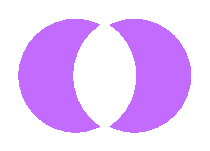
\includegraphics[height=3\baselineskip]{/home/emily/clowder-project/the-clowder-project/pictures/light-mode/symmetric-difference/definition/AsdiffB.pdf}}}%
                \hspace{0.5em}\scalebox{1.5}{$\mathbin{=}$}\hspace{0.5em}%
                \underset{\scalebox{1.25}{$\mkern7.0muU\setminus V$}}{\raisebox{-0.4\height}{
\includegraphics[height=3\baselineskip]{/home/emily/clowder-project/the-clowder-project/pictures/light-mode/symmetric-difference/definition/AsetminusB.pdf}}}%
                \hspace{0.5em}\scalebox{1.5}{$\mathbin{\cup}$}\hspace{0.5em}%
                \underset{\scalebox{1.25}{$\mkern7.0muV\setminus U$}}{\raisebox{-0.4\height}{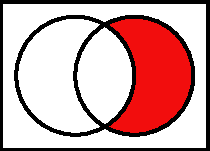
\includegraphics[height=3\baselineskip]{/home/emily/clowder-project/the-clowder-project/pictures/light-mode/symmetric-difference/definition/BsetminusA.pdf}}}%
                \mkern2.5mu.%
            $}%
        \end{webcompile}%%
    }%
    %---  End Footnote  ---%
    \[
        U\sdiff V
        \defeq
        (U\setminus V)%
        \cup%
        (V\setminus U).%
    \]%
\end{definition}
\begin{proposition}\label{constructions-with-sets:properties-of-symmetric-differences}%
    Let $X$ be a set.
    \begin{enumerate}
        \item\label{constructions-with-sets:properties-of-symmetric-differences-lack-of-functoriality}\SloganFont{Lack of Functoriality. }The assignment $(U,V)\mapsto U\sdiff V$ \demph{does not} in general define functors
            \[
                \BifunctorialityPeriod{U\sdiff-}{-\sdiff V}{-_{1}\sdiff-_{2}}{(\mathcal{P}(X),\subset)}{(\mathcal{P}(X),\subset)}{(\mathcal{P}(X)\times\mathcal{P}(X),\subset\times\subset)}{(\mathcal{P}(X),\subset)}%
            \]%
        \item\label{constructions-with-sets:properties-of-symmetric-differences-via-unions-and-intersections}\SloganFont{Via Unions and Intersections. }We have%
            \[
                U\sdiff V%
                =%
                (U\cup V)\setminus(U\cap V)%
            \]%
            for each $U,V\in\mathcal{P}(X)$, as in the Venn diagram
            \begin{webcompile}
                \underset{\scalebox{1.0}{$\mkern3.5muU\sdiff V$}}{\raisebox{-0.4\height}{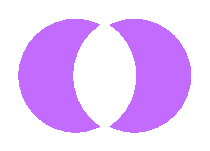
\includegraphics[height=2\baselineskip]{/home/emily/clowder-project/the-clowder-project/pictures/light-mode/symmetric-difference/via-unions-and-intersections/Venn0110.pdf}}}%
                \hspace{0.5em}\scalebox{1.5}{$\mathbin{=}$}\hspace{0.6em}%
                \underset{\scalebox{1.0}{$\mkern3.5muU\cup V$}}{\raisebox{-0.4\height}{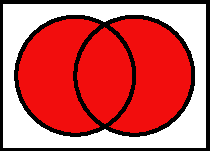
\includegraphics[height=2\baselineskip]{/home/emily/clowder-project/the-clowder-project/pictures/light-mode/symmetric-difference/via-unions-and-intersections/Venn0111.pdf}}}%
                \hspace{0.5em}\scalebox{1.5}{$\mathbin{\setminus}$}\hspace{0.5em}%
                \underset{\scalebox{1.0}{$\mkern3.5muU\cap V$}}{\raisebox{-0.4\height}{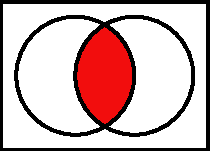
\includegraphics[height=2\baselineskip]{/home/emily/clowder-project/the-clowder-project/pictures/light-mode/symmetric-difference/via-unions-and-intersections/Venn0001.pdf}}}%
                \mkern2.5mu.%
            \end{webcompile}%%
        \item\label{constructions-with-sets:properties-of-symmetric-differences-symmetric-differences-of-disjoint-sets}\SloganFont{Symmetric Differences of Disjoint Sets. }If $U$ and $V$ are disjoint, then we have
            \[
                U\sdiff V%
                =%
                U\cup V.%
            \]%
        \item\label{constructions-with-sets:properties-of-symmetric-differences-associativity}\SloganFont{Associativity. }The diagram
            \[
                \begin{tikzcd}[row sep={0*\the\DL,between origins}, column sep={0*\the\DL,between origins}, background color=backgroundColor, ampersand replacement=\&]
                    \&[0.30901699437\TwoCmPlusHalf]
                    \&[0.5\TwoCmPlusHalf]
                    \mathcal{P}(X)\times(\mathcal{P}(X)\times\mathcal{P}(X))
                    \&[0.5\TwoCmPlusHalf]
                    \&[0.30901699437\TwoCmPlusHalf]
                    \\[0.58778525229\TwoCmPlusHalf]
                    (\mathcal{P}(X)\times\mathcal{P}(X))\times\mathcal{P}(X)
                    \&[0.30901699437\TwoCmPlusHalf]
                    \&[0.5\TwoCmPlusHalf]
                    \&[0.5\TwoCmPlusHalf]
                    \&[0.30901699437\TwoCmPlusHalf]
                    \mathcal{P}(X)\times\mathcal{P}(X)
                    \\[0.95105651629\TwoCmPlusHalf]
                    \&[0.30901699437\TwoCmPlusHalf]
                    \mathcal{P}(X)\times\mathcal{P}(X)
                    \&[0.5\TwoCmPlusHalf]
                    \&[0.5\TwoCmPlusHalf]
                    \mathcal{P}(X)\mrp{,}
                    \&[0.30901699437\TwoCmPlusHalf]
                    % 1-Arrows
                    % Left Boundary
                    \arrow[from=2-1,to=1-3,"\alpha^{\Sets}_{\mathcal{P}(X),\mathcal{P}(X),\mathcal{P}(X)}"{pos=0.35},isoarrowprime]%
                    \arrow[from=1-3,to=2-5,"{\id_{\mathcal{P}(X)}\times\mathord{\sdiff}}"{pos=0.55},""{name=2}]%
                    \arrow[from=2-5,to=3-4,"\sdiff"{pos=0.425}]%
                    % Right Boundary
                    \arrow[from=2-1,to=3-2,"{\mathord{\sdiff}\times\id_{\mathcal{P}(X)}}"'{pos=0.425}]%
                    \arrow[from=3-2,to=3-4,"\sdiff"']%
                \end{tikzcd}
            \]%
            commutes, i.e.\ we have%
            \[
                (U\sdiff V)\sdiff W
                =
                U\sdiff(V\sdiff W)
            \]%
            for each $U,V,W\in\mathcal{P}(X)$, as in the Venn diagram
            \begin{webcompile}
                \underset{\scalebox{1.0}{$\mkern3.75muU\sdiff V$}}{\raisebox{-0.4\height}{
\includegraphics[height=3\baselineskip]{/home/emily/clowder-project/the-clowder-project/pictures/light-mode/symmetric-difference/associativity/A_sdiff_B.pdf}}}%
                \hspace{0.5em}\scalebox{1.5}{$\mathbin{\sdiff}$}\hspace{0.5em}%
                \underset{\mcp{\scalebox{1.0}{$W$}}}{\raisebox{-0.4\height}{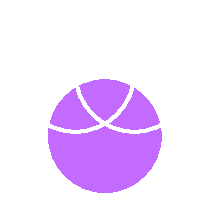
\includegraphics[height=3\baselineskip]{/home/emily/clowder-project/the-clowder-project/pictures/light-mode/symmetric-difference/associativity/C.pdf}}}%
                \hspace{0.5em}\scalebox{1.5}{$\mathbin{=}$}\hspace{0.3em}%
                \underset{\scalebox{1.0}{$U\sdiff V\sdiff W$}}{\raisebox{-0.4\height}{
\includegraphics[height=3\baselineskip]{/home/emily/clowder-project/the-clowder-project/pictures/light-mode/symmetric-difference/associativity/A_sdiff_B_sdiff_C.pdf}}}%
                \hspace{0.2em}\scalebox{1.5}{$\mathbin{=}$}\hspace{0.5em}%
                \underset{\mcp{\scalebox{1.0}{$U$}}}{\raisebox{-0.4\height}{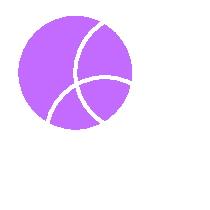
\includegraphics[height=3\baselineskip]{/home/emily/clowder-project/the-clowder-project/pictures/light-mode/symmetric-difference/associativity/A.pdf}}}%
                \hspace{0.5em}\scalebox{1.5}{$\mathbin{\sdiff}$}\hspace{0.5em}%
                \underset{\scalebox{1.0}{$\mkern4.25muV\sdiff W$}}{\raisebox{-0.4\height}{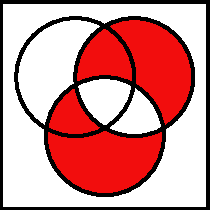
\includegraphics[height=3\baselineskip]{/home/emily/clowder-project/the-clowder-project/pictures/light-mode/symmetric-difference/associativity/B_sdiff_C.pdf}}}%
                \mkern2.5mu.%
            \end{webcompile}%%
        \item\label{constructions-with-sets:properties-of-symmetric-differences-unitality}\SloganFont{Unitality. }The diagrams
            \begin{webcompile}
                \begin{tikzcd}[row sep={5.0*\the\DL,between origins}, column sep={11.25*\the\DL,between origins}, background color=backgroundColor, ampersand replacement=\&]
                    \pt\times\mathcal{P}(X)
                    \arrow[r,"{[\emptyset]\times\id_{\mathcal{P}(X)}}"]
                    \arrow[rd,"\LUnitor^{\Sets}_{\mathcal{P}(X)}"',isoarrow]
                    \&
                    \mathcal{P}(X)\times\mathcal{P}(X)
                    \arrow[d,"\sdiff"]
                    \\
                    \&
                    \mathcal{P}(X)
                \end{tikzcd}
                \quad
                \begin{tikzcd}[row sep={5.0*\the\DL,between origins}, column sep={11.25*\the\DL,between origins}, background color=backgroundColor, ampersand replacement=\&]
                    \mathcal{P}(X)\times\pt
                    \arrow[r,"{\id_{\mathcal{P}(X)}\times[\emptyset]}"]
                    \arrow[rd,"\RUnitor^{\Sets}_{\mathcal{P}(X)}"',isoarrow]
                    \&
                    \mathcal{P}(X)\times\mathcal{P}(X)
                    \arrow[d,"\sdiff"]
                    \\
                    \&
                    \mathcal{P}(X)
                \end{tikzcd}
            \end{webcompile}
            commute, i.e.\ we have
            \begin{align*}
                U\sdiff\emptyset  &= U,\\
                \emptyset\sdiff U &= U
            \end{align*}
            for each $U\in\mathcal{P}(X)$.
        \item\label{constructions-with-sets:properties-of-symmetric-differences-commutativity}\SloganFont{Commutativity. }The diagram
            \[
                \begin{tikzcd}[row sep={5.0*\the\DL,between origins}, column sep={12.0*\the\DL,between origins}, background color=backgroundColor, ampersand replacement=\&]
                    \mathcal{P}(X)\times\mathcal{P}(X)
                    \arrow[r,"\sigma^{\Sets}_{\mathcal{P}(X),\mathcal{P}(X)}"]
                    \arrow[rd,"\sdiff"']
                    \&
                    \mathcal{P}(X)\times\mathcal{P}(X)
                    \arrow[d,"\sdiff"]
                    \\
                    \&
                    \mathcal{P}(X)
                \end{tikzcd}
            \]%
            commutes, i.e.\ we have
            \[
                U\sdiff V
                =
                V\sdiff U
            \]%
            for each $U,V\in\mathcal{P}(X)$.
        \item\label{constructions-with-sets:properties-of-symmetric-differences-invertibility}\SloganFont{Invertibility. }We have
            \[
                U\sdiff U
                =
                \emptyset
            \]%
            for each $U\in\mathcal{P}(X)$.
        \item\label{constructions-with-sets:properties-of-symmetric-differences-interaction-with-unions}\SloganFont{Interaction With Unions. }We have
            \[
                (U\sdiff V)\cup(V\sdiff T)
                =
                (U\cup V\cup W)\setminus(U\cap V\cap W)
            \]%
            for each $U,V,W\in\mathcal{P}(X)$.
        \item\label{constructions-with-sets:properties-of-symmetric-differences-interaction-with-complements-1}\SloganFont{Interaction With Complements \rmI. }We have
            \[
                U\sdiff U^{\sfc}%
                =
                X%
            \]%
            for each $U\in\mathcal{P}(X)$.
        \item\label{constructions-with-sets:properties-of-symmetric-differences-interaction-with-complements-2}\SloganFont{Interaction With Complements \rmII. }We have
            \begin{align*}
                U\sdiff X &= U^{\sfc},\\%
                X\sdiff U &= U^{\sfc}%
            \end{align*}
            for each $U\in\mathcal{P}(X)$.
        \item\label{constructions-with-sets:properties-of-symmetric-differences-interaction-with-complements-3}\SloganFont{Interaction With Complements \rmIII. }The diagram
            \[
                \begin{tikzcd}[row sep={5.0*\the\DL,between origins}, column sep={8.0*\the\DL,between origins}, background color=backgroundColor, ampersand replacement=\&]
                    \mathcal{P}(X)\times\mathcal{P}(X)
                    \arrow[r,"\sdiff"]
                    \arrow[d,"{(-)^{\sfc}\times(-)^{\sfc}}"']
                    \&
                    \mathcal{P}(X)
                    \arrow[d,"{(-)^{\sfc}}"]
                    \\
                    \mathcal{P}(X)\times\mathcal{P}(X)
                    \arrow[r,"\sdiff"']
                    \&
                    \mathcal{P}(X)
                \end{tikzcd}
            \]%
            commutes, i.e.\ we have
            \[
                U^{\sfc}\sdiff V^{\sfc}%
                =%
                U\sdiff V%
            \]%
            for each $U,V\in\mathcal{P}(X)$.
        \item\label{constructions-with-sets:properties-of-symmetric-differences-transitivity}\SloganFont{``Transitivity''. }We have
            \[
                (U\sdiff V)\sdiff(V\sdiff W)%
                =%
                U\sdiff W%
            \]%
            for each $U,V,W\in\mathcal{P}(X)$.
        \item\label{constructions-with-sets:properties-of-symmetric-differences-the-triangle-inequality-for-symmetric-differences}\SloganFont{The Triangle Inequality for Symmetric Differences. }We have
            \[
                U\sdiff W%
                \subset%
                U\sdiff V%
                \cup
                V\sdiff W%
            \]%
            for each $U,V,W\in\mathcal{P}(X)$.
        \item\label{constructions-with-sets:properties-of-symmetric-differences-distributivity-over-intersections}\SloganFont{Distributivity Over Intersections. }We have
            \begin{align*}
                U\cap(V\sdiff W)  &= (U\cap V)\sdiff(U\cap W),\\
                (U\sdiff V)\cap W &= (U\cap W)\sdiff(V\cap W)
            \end{align*}
            for each $U,V,W\in\mathcal{P}(X)$.
        \item\label{constructions-with-sets:properties-of-symmetric-differences-interaction-with-characteristic-functions}\SloganFont{Interaction With Characteristic Functions. }We have
            \[
                \chi_{U\sdiff V}%
                =%
                \chi_{U}%
                +%
                \chi_{V}%
                -%
                2\chi_{U\cap V}%
            \]%
            and thus, in particular, we have
            \[
                \chi_{U\sdiff V}%
                \equiv%
                \chi_{U}+\chi_{V}%
                \mod{2}%
            \]%
            for each $U,V\in\mathcal{P}(X)$.
        \item\label{constructions-with-sets:properties-of-symmetric-differences-bijectivity}\SloganFont{Bijectivity. }Given $U,V\in\mathcal{P}(X)$, the maps
            \begin{align*}
                U\sdiff-  &\colon \mathcal{P}(X) \to \mathcal{P}(X),\\
                -\sdiff V &\colon \mathcal{P}(X) \to \mathcal{P}(X)
            \end{align*}
            are bijections with inverses given by
            \begin{align*}
                (U\sdiff-)^{-1}  &= -\cup(U\cap-),\\
                (-\sdiff V)^{-1} &= -\cup(V\cap-).
            \end{align*}
            Moreover, the map
            \begin{webcompile}
                \begin{tikzcd}[row sep=0.0*\the\DL, column sep=1.0*\the\DL, background color=backgroundColor, ampersand replacement=\&]
                    \mathcal{P}(X)
                    \arrow[r]
                    \&
                    \mathcal{P}(X)
                    \\
                    C
                    \arrow[r, mapsto]
                    \&
                    C\sdiff(U\sdiff V)%
                \end{tikzcd}
            \end{webcompile}%
            is a bijection of $\mathcal{P}(X)$ onto itself sending $U$ to $V$ and $V$ to $U$.
        \item\label{constructions-with-sets:properties-of-symmetric-differences-interaction-with-powersets-and-groups}\SloganFont{Interaction With Powersets and Groups. }Let $X$ be a set.
            \begin{enumerate}
                \item\label{constructions-with-sets:properties-of-symmetric-differences-interaction-with-powersets-and-groups-a}The quadruple $(\mathcal{P}(X),\sdiff,\emptyset,\id_{\mathcal{P}(X)})$ is an abelian group.%
                    %--- Begin Footnote ---%
                    \footnote{%
                        Here are some examples:
                        \begin{enumerate}
                            \item When $X=\emptyset$, we have an isomorphism of groups between $\mathcal{P}(\emptyset)$ and the trivial group:
                                \[
                                    (\mathcal{P}(\emptyset),\sdiff,\emptyset,\id_{\mathcal{P}(\emptyset)})
                                    \cong
                                    \pt.
                                \]%
                            \item When $X=\pt$, we have an isomorphism of groups between $\mathcal{P}(\pt)$ and $\Zn{2}$:
                                \[
                                    (\mathcal{P}(\pt),\sdiff,\emptyset,\id_{\mathcal{P}(\pt)})
                                    \cong
                                    \Zn{2}.
                                \]%
                            \item When $X=\left\{0,1\right\}$, we have an isomorphism of groups between $\mathcal{P}(\left\{0,1\right\})$ and $\Zn{2}\times\Zn{2}$:
                                \[
                                    (\mathcal{P}(\left\{0,1\right\}),\sdiff,\emptyset,\id_{\mathcal{P}(\left\{0,1\right\})})
                                    \cong
                                    \Zn{2}\times\Zn{2}.
                                \]%
                        \end{enumerate}
                    }%
                    %---  End Footnote  ---%
                \item\label{constructions-with-sets:properties-of-symmetric-differences-interaction-with-powersets-and-groups-b}Every element of $\mathcal{P}(X)$ has order $2$ with respect to $\sdiff$, and thus $\mathcal{P}(X)$ is a \emph{Boolean group} (i.e.\ an abelian $2$-group).
            \end{enumerate}
        \item\label{constructions-with-sets:properties-of-symmetric-differences-interaction-with-powersets-and-vector-spaces-1}\SloganFont{Interaction With Powersets and Vector Spaces \rmI. }The pair $(\mathcal{P}(X),\alpha_{\mathcal{P}(X)})$ consisting of
            \begin{itemize}
                \item The group $\mathcal{P}(X)$ of \cref{constructions-with-sets:properties-of-symmetric-differences-interaction-with-powersets-and-groups};
                \item The map $\alpha_{\mathcal{P}(X)}\colon\F_{2}\times\mathcal{P}(X)\to\mathcal{P}(X)$ defined by
                    \begin{align*}
                        0\cdot U &\defeq \emptyset,\\
                        1\cdot U &\defeq U;
                    \end{align*}
            \end{itemize}
            is an $\F_{2}$-vector space.
        \item\label{constructions-with-sets:properties-of-symmetric-differences-interaction-with-powersets-and-vector-spaces-2}\SloganFont{Interaction With Powersets and Vector Spaces \rmII. }If $X$ is finite, then:
            \begin{enumerate}% PROCESS %
                \item The set of singletons sets on the elements of $X$ forms a basis for the $\F_{2}$-vector space $(\mathcal{P}(X),\alpha_{\mathcal{P}(X)})$ of \cref{constructions-with-sets:properties-of-symmetric-differences-interaction-with-powersets-and-vector-spaces-1}.
                \item We have
                    \[
                        \dim(\mathcal{P}(X))%
                        =%
                        \Card{X}.%
                    \]%
            \end{enumerate}% PROCESS %
        \item\label{constructions-with-sets:properties-of-symmetric-differences-interaction-with-powersets-and-rings}\SloganFont{Interaction With Powersets and Rings. }The quintuple $(\mathcal{P}(X),\sdiff,\cap,\emptyset,X)$ is a commutative ring.%
            %--- Begin Footnote ---%
            \footnote{%
                \textdbend\SloganFont{Warning: }The analogous statement replacing intersections by unions (i.e.\ that the quintuple $(\mathcal{P}(X),\sdiff,\cup,\emptyset,X)$ is a ring) is false, however. See \cite{proof-wiki:symmetric-difference-with-union-does-not-form-ring} for a proof.

                END TEXTDBEND
            }%
            %---  End Footnote  ---%
        \item\label{constructions-with-sets:properties-of-symmetric-differences-interaction-with-direct-images}\SloganFont{Interaction With Direct Images. }We have a natural transformation
            \[
                \begin{tikzcd}[row sep={5.0*\the\DL,between origins}, column sep={11.5*\the\DL,between origins}, background color=backgroundColor, ampersand replacement=\&]
                    \mathcal{P}(X)^{\op}\times\mathcal{P}(X)
                    \arrow[r,"f^{\op}_{*}\times f_{*}"]
                    \arrow[d,"\sdiff"']
                    \&
                    \mathcal{P}(Y)^{\op}\times\mathcal{P}(Y)
                    \arrow[d,"\sdiff"]
                    \\
                    \mathcal{P}(X)
                    \arrow[r,"f_{*}"']
                    \&
                    \mathcal{P}(Y)
                    % 2-Arrows
                    \arrow[from=1-2,to=2-1,"\scalebox{1.5}{$\supset$}"{sloped,description},phantom,shorten <= 0.5*\the\DL,shorten >= 0.625*\the\DL,Rightarrow,pos=0.5]%
                \end{tikzcd}
            \]%
            with components
            \[
                f_{*}(U)\sdiff f_{*}(V)%
                \subset%
                f_{*}(U\sdiff V)%
            \]%
            indexed by $U,V\in\mathcal{P}(X)$.
        \item\label{constructions-with-sets:properties-of-symmetric-differences-interaction-with-inverse-images}\SloganFont{Interaction With Inverse Images. }The diagram
            \[
                \begin{tikzcd}[row sep={5.0*\the\DL,between origins}, column sep={13.0*\the\DL,between origins}, background color=backgroundColor, ampersand replacement=\&]
                    \mathcal{P}(Y)^{\op}\times\mathcal{P}(Y)
                    \arrow[r,"f^{\op,-1}\times f^{-1}"]
                    \arrow[d,"\sdiff"']
                    \&
                    \mathcal{P}(X)^{\op}\times\mathcal{P}(X)
                    \arrow[d,"\sdiff"]
                    \\
                    \mathcal{P}(Y)
                    \arrow[r,"f^{-1}"']
                    \&
                    \mathcal{P}(X)
                \end{tikzcd}
            \]%
            i.e.\ we have
            \[
                f^{-1}(U)\sdiff f^{-1}(V)%
                =%
                f^{-1}(U\sdiff V)%
            \]%
            for each $U,V\in\mathcal{P}(Y)$.
        \item\label{constructions-with-sets:properties-of-symmetric-differences-interaction-with-direct-images-with-compact-support}\SloganFont{Interaction With Direct Images With Compact Support. }We have a natural transformation
            \[
                \begin{tikzcd}[row sep={5.0*\the\DL,between origins}, column sep={11.5*\the\DL,between origins}, background color=backgroundColor, ampersand replacement=\&]
                    \mathcal{P}(X)^{\op}\times\mathcal{P}(X)
                    \arrow[r,"f^{\op}_{!}\times f_{!}"]
                    \arrow[d,"\sdiff"']
                    \&
                    \mathcal{P}(Y)^{\op}\times\mathcal{P}(Y)
                    \arrow[d,"\sdiff"]
                    \\
                    \mathcal{P}(X)
                    \arrow[r,"f_{!}"']
                    \&
                    \mathcal{P}(Y)
                    % 2-Arrows
                    \arrow[from=2-1,to=1-2,"\scalebox{1.5}{$\supset$}"{sloped,description},phantom,shorten <= 0.5*\the\DL,shorten >= 0.625*\the\DL,Rightarrow,pos=0.5]%
                \end{tikzcd}
            \]%
            with components
            \[
                f_{!}(U\sdiff V)%
                \subset%
                f_{1}(U)\sdiff f_{!}(V)%
            \]%
            indexed by $U,V\in\mathcal{P}(X)$.
    \end{enumerate}
\end{proposition}
\begin{proof}
    \textit{\cref{constructions-with-sets:properties-of-symmetric-differences-lack-of-functoriality}, Lack of Functoriality}:
    Omitted.

    \textit{\cref{constructions-with-sets:properties-of-symmetric-differences-via-unions-and-intersections}, Via Unions and Intersections}:
    See \cite{proof-wiki:equivalence-of-definitions-of-symmetric-difference}.

    \textit{\cref{constructions-with-sets:properties-of-symmetric-differences-symmetric-differences-of-disjoint-sets}, Symmetric Differences of Disjoint Sets}:
    Since $U$ and $V$ are disjoint, we have $U\cap V=\emptyset$, and therefore we have
    \begin{align*}
        U\sdiff V &= (U\cup V)\setminus(U\cap V)\\
                  &= (U\cup V)\setminus\emptyset\\
                  &= U\cup V,
    \end{align*}
    where we've used \cref{constructions-with-sets:properties-of-symmetric-differences-via-unions-and-intersections} and \cref{constructions-with-sets:properties-of-differences-right-unitality} of \cref{constructions-with-sets:properties-of-differences}.

    \textit{\cref{constructions-with-sets:properties-of-symmetric-differences-associativity}, Associativity}:
    See \cite{proof-wiki:symmetric-difference-is-associative}.

    \textit{\cref{constructions-with-sets:properties-of-symmetric-differences-unitality}, Unitality}:
    This follows from \cref{constructions-with-sets:properties-of-symmetric-differences-commutativity} and \cite{proof-wiki:symmetric-difference-with-empty-set}.

    \textit{\cref{constructions-with-sets:properties-of-symmetric-differences-commutativity}, Commutativity}:
    See \cite{proof-wiki:symmetric-difference-is-commutative}.

    \textit{\cref{constructions-with-sets:properties-of-symmetric-differences-invertibility}, Invertibility}:
    See \cite{proof-wiki:symmetric-difference-with-self-is-empty-set}.

    \textit{\cref{constructions-with-sets:properties-of-symmetric-differences-interaction-with-unions}, Interaction With Unions}:
    See \cite{proof-wiki:union-of-symmetric-differences}.

    \textit{\cref{constructions-with-sets:properties-of-symmetric-differences-interaction-with-complements-1}, Interaction With Complements \rmI}:
    See \cite{proof-wiki:symmetric-difference-with-complement}.

    \textit{\cref{constructions-with-sets:properties-of-symmetric-differences-interaction-with-complements-2}, Interaction With Complements \rmII}:
    This follows from \cref{constructions-with-sets:properties-of-symmetric-differences-commutativity} and \cite{proof-wiki:symmetric-difference-with-universe}.

    \textit{\cref{constructions-with-sets:properties-of-symmetric-differences-interaction-with-complements-3}, Interaction With Complements \rmIII}:
    See \cite{proof-wiki:symmetric-difference-of-complements}.

    \textit{\cref{constructions-with-sets:properties-of-symmetric-differences-transitivity}, ``Transitivity''}:
    We have
    \begin{align*}
        (U\sdiff V)\sdiff(V\sdiff W) &= U\sdiff(V\sdiff(V\sdiff W))  \ptag{by \cref{constructions-with-sets:properties-of-symmetric-differences-associativity}}\\
                                     &= U\sdiff((V\sdiff V)\sdiff W) \ptag{by \cref{constructions-with-sets:properties-of-symmetric-differences-associativity}}\\
                                     &= U\sdiff(\emptyset\sdiff W)   \ptag{by \cref{constructions-with-sets:properties-of-symmetric-differences-invertibility}}\\
                                     &= U\sdiff W.                   \ptag{by \cref{constructions-with-sets:properties-of-symmetric-differences-unitality}}
    \end{align*}
    This finishes the proof.

    \textit{\cref{constructions-with-sets:properties-of-symmetric-differences-the-triangle-inequality-for-symmetric-differences}, The Triangle Inequality for Symmetric Differences}:
    This follows from \cref{constructions-with-sets:properties-of-symmetric-differences-transitivity,constructions-with-sets:properties-of-symmetric-differences-via-unions-and-intersections}.

    \textit{\cref{constructions-with-sets:properties-of-symmetric-differences-distributivity-over-intersections}, Distributivity Over Intersections}:
    See \cite{proof-wiki:intersection-distributes-over-symmetric-difference}.

    \textit{\cref{constructions-with-sets:properties-of-symmetric-differences-interaction-with-characteristic-functions}, Interaction With Characteristic Functions}:
    See \cite{proof-wiki:characteristic-function-of-symmetric-difference}.

    \textit{\cref{constructions-with-sets:properties-of-symmetric-differences-bijectivity}, Bijectivity}:
    Omitted.

    \textit{\cref{constructions-with-sets:properties-of-symmetric-differences-interaction-with-powersets-and-groups}, Interaction With Powersets and Groups}:
    \cref{constructions-with-sets:properties-of-symmetric-differences-interaction-with-powersets-and-groups-a} follows from \cref{constructions-with-sets:properties-of-symmetric-differences-associativity,constructions-with-sets:properties-of-symmetric-differences-unitality,constructions-with-sets:properties-of-symmetric-differences-invertibility,constructions-with-sets:properties-of-symmetric-differences-commutativity}, while \cref{constructions-with-sets:properties-of-symmetric-differences-interaction-with-powersets-and-groups-b} follows from \cref{constructions-with-sets:properties-of-symmetric-differences-invertibility}.%
    %--- Begin Footnote ---%
    \footnote{%
        \SloganFont{Reference: }: \cite{proof-wiki:symmetric-difference-on-power-set-forms-abelian-group}.
    }%
    %---  End Footnote  ---%

    \textit{\cref{constructions-with-sets:properties-of-symmetric-differences-interaction-with-powersets-and-vector-spaces-1}, Interaction With Powersets and Vector Spaces \rmI}:
    See \cite{MSE2719059}.

    \textit{\cref{constructions-with-sets:properties-of-symmetric-differences-interaction-with-powersets-and-vector-spaces-2}, Interaction With Powersets and Vector Spaces \rmII}:
    See \cite{MSE2719059}.

    \textit{\cref{constructions-with-sets:properties-of-symmetric-differences-interaction-with-powersets-and-rings}, Interaction With Powersets and Rings}:
    This follows from \cref{constructions-with-sets:properties-of-binary-intersections-annihilation-with-the-empty-set,constructions-with-sets:properties-of-binary-intersections-interaction-with-powersets-and-monoids-with-zero} of \cref{constructions-with-sets:properties-of-binary-intersections} and \cref{constructions-with-sets:properties-of-symmetric-differences-distributivity-over-intersections,constructions-with-sets:properties-of-symmetric-differences-interaction-with-powersets-and-groups}.%
    %--- Begin Footnote ---%
    \footnote{%
        \SloganFont{Reference: }\cite{proof-wiki:symmetric-difference-with-intersection-forms-ring}.
    }%
    %---  End Footnote  ---%

    \textit{\cref{constructions-with-sets:properties-of-symmetric-differences-interaction-with-direct-images}, Interaction With Direct Images}:
    This is a repetition of \cref{constructions-with-sets:properties-of-direct-images-i-interaction-with-symmetric-differences} of \cref{constructions-with-sets:properties-of-direct-images-i} and is proved there.

    \textit{\cref{constructions-with-sets:properties-of-symmetric-differences-interaction-with-inverse-images}, Interaction With Inverse Images}:
    This is a repetition of \cref{constructions-with-sets:properties-of-inverse-images-i-interaction-with-symmetric-differences} of \cref{constructions-with-sets:properties-of-inverse-images-i} and is proved there.

    \textit{\cref{constructions-with-sets:properties-of-symmetric-differences-interaction-with-direct-images-with-compact-support}, Interaction With Direct Images With Compact Support}:
    This is a repetition of \cref{constructions-with-sets:properties-of-direct-images-with-compact-support-i-interaction-with-symmetric-differences} of \cref{constructions-with-sets:properties-of-direct-images-with-compact-support-i} and is proved there.
\end{proof}
\section{Powersets}\label{constructions-with-sets:section-powersets}
\subsection{Foundations}\label{constructions-with-sets:subsection-powersets-foundations}
Let $X$ be a set.%
\begin{definition}\label{constructions-with-sets:powersets}%
    The \index[set-theory]{powerset}\textbf{powerset of $X$} is the set \index[notation]{PX@$\mathcal{P}(X)$}$\mathcal{P}(X)$ defined by
    \[
        \mathcal{P}(X)
        \defeq
        \left\{%
            U\in P%
            \ \middle|\ %
            U\subset X%
        \right\},
    \]%
    where $P$ is the set in the axiom of powerset, \cref{constructions-with-sets:zermelo-fraenkel-set-theory-the-axiom-of-powerset} of \cref{constructions-with-sets:zermelo-fraenkel-set-theory}.
\end{definition}
\begin{remark}\label{constructions-with-sets:powersets-as-decategorifications-of-co-presheaf-categories}%
    Under the analogy that $\TTV$ should be the $(-1)$-categorical analogue of $\Sets$, we may view the powerset of a set as a decategorification of the category of presheaves of a category (or of the category of copresheaves):%
    \begin{itemize}
        \item The powerset of a set $X$ is equivalently (\cref{constructions-with-sets:properties-of-characteristic-functions-of-subsets-bijectivity} of \cref{constructions-with-sets:properties-of-characteristic-functions-of-subsets}) the set
            \[%
                \Sets(X,\TTV)
            \]%
            of functions from $X$ to the set $\TTV$ of classical truth values.
        \item The category of presheaves on a category $\CatFont{C}$ is the category
            \[%
                \Fun(\CatFont{C}^{\op},\Sets)%
            \]%
            of functors from $\CatFont{C}^{\op}$ to the category $\Sets$ of sets.
    \end{itemize}
\end{remark}
\begin{notation}\label{constructions-with-sets:further-notation-for-powersets}%
    Let $X$ be a set.
    \begin{enumerate}
        \item\label{constructions-with-sets:further-notation-for-powersets-nonempty-powersets}We write \index[notation]{P0X@$\mathcal{P}_{0}(X)$}$\mathcal{P}_{0}(X)$ for the set of nonempty subsets of $X$.
        \item\label{constructions-with-sets:further-notation-for-powersets-finite-powersets}We write \index[notation]{PfinX@$\mathcal{P}_{\fin}(X)$}$\mathcal{P}_{\fin}(X)$ for the set of finite subsets of $X$.
    \end{enumerate}
\end{notation}
\begin{proposition}\label{constructions-with-sets:elementary-properties-of-powersets}%
    Let $X$ be a set.
    \begin{enumerate}
        \item\label{constructions-with-sets:elementary-properties-of-powersets-co-completeness}\SloganFont{Co/Completeness. }The (posetal) category (associated to) $(\mathcal{P}(X),\subset)$ is complete and cocomplete:
            \begin{enumerate}
                \item\SloganFont{Products. }The products in $\mathcal{P}(X)$ are given by intersection of subsets.
                \item\SloganFont{Coproducts. }The coproducts in $\mathcal{P}(X)$ are given by union of subsets.
                \item\SloganFont{Co/Equalisers. }Being a posetal category, $\mathcal{P}(X)$ only has at most one morphisms between any two objects, so co/equalisers are trivial.
            \end{enumerate}
        \item\label{constructions-with-sets:elementary-properties-of-powersets-cartesian-closedness}\SloganFont{Cartesian Closedness. }The category $\mathcal{P}(X)$ is Cartesian closed.
        \item\label{constructions-with-sets:elementary-properties-of-powersets-powersets-as-sets-of-relations}\SloganFont{Powersets as Sets of Relations. }We have bijections
            \begin{align*}
                \mathcal{P}(X) &\cong \Rel(\pt,X),\\
                \mathcal{P}(X) &\cong \Rel(X,\pt),
            \end{align*}
            natural in $X\in\Obj(\Sets)$.
        \item\label{constructions-with-sets:properties-of-powersets-as-categories-interaction-with-products-1}\SloganFont{Interaction With Products \rmI. }The map
            \begin{webcompile}
                \begin{tikzcd}[row sep=0.0*\the\DL, column sep=1.5*\the\DL, background color=backgroundColor, ampersand replacement=\&]
                    \mathcal{P}(X)\times\mathcal{P}(Y)%
                    \arrow[r]
                    \&
                    \mathcal{P}(X\icoprod Y)
                    \\
                    {(U,V)}
                    \arrow[r, mapsto]
                    \&
                    {U\cup V}
                \end{tikzcd}
            \end{webcompile}%
            is an isomorphism of sets, natural in $X,Y\in\Obj(\Sets)$ with respect to each of the functor structures $\mathcal{P}_{*}$, $\mathcal{P}^{-1}$, and $\mathcal{P}_{!}$ on $\mathcal{P}$ of \cref{constructions-with-sets:functoriality-of-powersets}. Moreover, this makes $\mathcal{P}_{*}$, $\mathcal{P}^{-1}$, and $\mathcal{P}_{!}$ into symmetric monoidal functors.
        \item\label{constructions-with-sets:properties-of-powersets-as-categories-interaction-with-products-2}\SloganFont{Interaction With Products \rmII. }The map
            \begin{webcompile}
                \begin{tikzcd}[row sep=0.0*\the\DL, column sep=1.5*\the\DL, background color=backgroundColor, ampersand replacement=\&]
                    \mathcal{P}(X)\times\mathcal{P}(Y)%
                    \arrow[r]
                    \&
                    \mathcal{P}(X\icoprod Y)
                    \\
                    {(U,V)}
                    \arrow[r, mapsto]
                    \&
                    {U\boxtimes_{X\times Y}V\mrp{,}}
                \end{tikzcd}
            \end{webcompile}%
            where\index[notation]{UboxtimesXYV@$U\boxtimes_{X\times Y}V$}%
            \[
                U\boxtimes_{X\times Y}V%
                \defeq%
                \left\{%
                    (u,v)\in X\times Y%
                    \ \middle|\ %
                    \text{$u\in U$ and $v\in V$}%
                \right\}%
            \]%
            is an inclusion of sets, natural in $X,Y\in\Obj(\Sets)$ with respect to each of the functor structures $\mathcal{P}_{*}$, $\mathcal{P}^{-1}$, and $\mathcal{P}_{!}$ on $\mathcal{P}$ of \cref{constructions-with-sets:functoriality-of-powersets}. Moreover, this makes $\mathcal{P}_{*}$, $\mathcal{P}^{-1}$, and $\mathcal{P}_{!}$ into symmetric monoidal functors.
        \item\label{constructions-with-sets:properties-of-powersets-as-categories-interaction-with-products-3}\SloganFont{Interaction With Products \rmIII. }We have an isomorphism
            \[
                \mathcal{P}(X)\otimes\mathcal{P}(Y)%
                \cong
                \mathcal{P}(X\times Y),%
            \]%
            natural in $X,Y\in\Obj(\Sets)$ with respect to each of the functor structures $\mathcal{P}_{*}$, $\mathcal{P}^{-1}$, and $\mathcal{P}_{!}$ on $\mathcal{P}$ of \cref{constructions-with-sets:functoriality-of-powersets}, where $\otimes$ denotes the tensor product of suplattices of \cref{constructions-with-sets:TODO}. Moreover, this makes $\mathcal{P}_{*}$, $\mathcal{P}^{-1}$, and $\mathcal{P}_{!}$ into symmetric monoidal functors.
    \end{enumerate}
\end{proposition}
\begin{proof}
    \textit{\cref{constructions-with-sets:elementary-properties-of-powersets-co-completeness}, Co/Completeness}:
    Omitted.

    \textit{\cref{constructions-with-sets:elementary-properties-of-powersets-cartesian-closedness}, Cartesian Closedness}:
    See \cref{constructions-with-sets:subsection-the-internal-hom-of-a-powerset}.

    \textit{\cref{constructions-with-sets:elementary-properties-of-powersets-powersets-as-sets-of-relations}, Powersets as Sets of Relations}:
    Indeed, we have
    \begin{align*}
        \Rel(\pt,X) &\defeq \mathcal{P}(\pt\times X)\\
                    &\cong  \mathcal{P}(X)
    \end{align*}
    and
    \begin{align*}
        \Rel(X,\pt) &\defeq \mathcal{P}(X\times\pt)\\
                    &\cong  \mathcal{P}(X),
    \end{align*}
    where we have used \cref{constructions-with-sets:properties-of-products-of-sets-unitality} of  \cref{constructions-with-sets:properties-of-products-of-sets}.

    \textit{\cref{constructions-with-sets:properties-of-powersets-as-categories-interaction-with-products-1}, Interaction With Products \rmI}:
    The inverse of the map in the statement is the map
    \[
        \Phi%
        \colon%
        \mathcal{P}(X\icoprod Y)%
        \to%
        \mathcal{P}(X)\times\mathcal{P}(Y)%
    \]%
    defined by
    \[
        \Phi(S)%
        \defeq%
        (S_{X},S_{Y})%
    \]%
    for each $S\in\mathcal{P}(X\icoprod Y)$, where
    \begin{align*}
        S_{X} &\defeq \left\{x\in X\ \middle|\ (0,x)\in S\right\}\\
        S_{Y} &\defeq \left\{y\in Y\ \middle|\ (1,y)\in S\right\}.
    \end{align*}
    The rest of the proof is omitted.

    \textit{\cref{constructions-with-sets:properties-of-powersets-as-categories-interaction-with-products-2}, Interaction With Products \rmII}:
    Omitted.

    \textit{\cref{constructions-with-sets:properties-of-powersets-as-categories-interaction-with-products-3}, Interaction With Products \rmIII}:
    Omitted.
\end{proof}
\subsection{Functoriality of Powersets}\label{constructions-with-sets:subsection-functoriality-of-powersets}
\begin{proposition}\label{constructions-with-sets:functoriality-of-powersets}%
    Let $X$ be a set.
    \begin{enumerate}
        \item\label{constructions-with-sets:functoriality-of-powersets-functoriality-1}\SloganFont{Functoriality \rmI. }The assignment $X\mapsto\mathcal{P}(X)$ defines a functor\index[notation]{Pstar@$\mathcal{P}_{*}$}
            \[
                \mathcal{P}_{*}%
                \colon%
                \Sets%
                \to%
                \Sets,%
            \]%
            where
            \begin{itemize}
                \item\SloganFont{Action on Objects. }For each $A\in\Obj(\Sets)$, we have
                    \[
                        \mathcal{P}_{*}(A)%
                        \defeq%
                        \mathcal{P}(A).%
                    \]%
                \item\SloganFont{Action on Morphisms. }For each $A,B\in\Obj(\Sets)$, the action on morphisms
                    \[
                        \mathcal{P}_{*|A,B}%
                        \colon%
                        \Sets(A,B)%
                        \to%
                        \Sets(\mathcal{P}(A),\mathcal{P}(B))%
                    \]%
                    of $\mathcal{P}_{*}$ at $(A,B)$ is the map defined by by sending a map of sets $f\colon A\to B$ to the map
                    \[
                        \mathcal{P}_{*}(f)%
                        \colon%
                        \mathcal{P}(A)%
                        \to%
                        \mathcal{P}(B)%
                    \]%
                    defined by
                    \[
                        \mathcal{P}_{*}(f)%
                        \defeq%
                        f_{*},%
                    \]%
                    as in \cref{constructions-with-sets:the-direct-image-function-associated-to-a-function}.
            \end{itemize}
        \item\label{constructions-with-sets:functoriality-of-powersets-functoriality-2}\SloganFont{Functoriality \rmII. }The assignment $X\mapsto\mathcal{P}(X)$ defines a functor\index[notation]{Pminusone@$\mathcal{P}^{-1}$}
            \[
                \mathcal{P}^{-1}%
                \colon%
                \Sets^{\op}%
                \to%
                \Sets,%
            \]%
            where
            \begin{itemize}
                \item\SloganFont{Action on Objects. }For each $A\in\Obj(\Sets)$, we have
                    \[
                        \mathcal{P}^{-1}(A)%
                        \defeq%
                        \mathcal{P}(A).%
                    \]%
                \item\SloganFont{Action on Morphisms. }For each $A,B\in\Obj(\Sets)$, the action on morphisms
                    \[
                        \mathcal{P}^{-1}_{A,B}%
                        \colon%
                        \Sets(A,B)%
                        \to%
                        \Sets(\mathcal{P}(B),\mathcal{P}(A))%
                    \]%
                    of $\mathcal{P}^{-1}$ at $(A,B)$ is the map defined by by sending a map of sets $f\colon A\to B$ to the map
                    \[
                        \mathcal{P}^{-1}(f)%
                        \colon%
                        \mathcal{P}(B)%
                        \to%
                        \mathcal{P}(A)%
                    \]%
                    defined by
                    \[
                        \mathcal{P}^{-1}(f)%
                        \defeq%
                        f^{-1},%
                    \]%
                    as in \cref{constructions-with-sets:the-inverse-image-function-associated-to-a-function}.
            \end{itemize}
        \item\label{constructions-with-sets:functoriality-of-powersets-functoriality-3}\SloganFont{Functoriality \rmIII. }The assignment $X\mapsto\mathcal{P}(X)$ defines a functor\index[notation]{Pshriek@$\mathcal{P}_{"!}$}
            \[
                \mathcal{P}_{!}%
                \colon%
                \Sets%
                \to%
                \Sets,%
            \]%
            where
            \begin{itemize}
                \item\SloganFont{Action on Objects. }For each $A\in\Obj(\Sets)$, we have
                    \[
                        \mathcal{P}_{!}(A)%
                        \defeq%
                        \mathcal{P}(A).%
                    \]%
                \item\SloganFont{Action on Morphisms. }For each $A,B\in\Obj(\Sets)$, the action on morphisms
                    \[
                        \mathcal{P}_{!|A,B}%
                        \colon%
                        \Sets(A,B)%
                        \to%
                        \Sets(\mathcal{P}(A),\mathcal{P}(B))%
                    \]%
                    of $\mathcal{P}_{!}$ at $(A,B)$ is the map defined by by sending a map of sets $f\colon A\to B$ to the map
                    \[
                        \mathcal{P}_{!}(f)%
                        \colon%
                        \mathcal{P}(A)%
                        \to%
                        \mathcal{P}(B)%
                    \]%
                    defined by
                    \[
                        \mathcal{P}_{!}(f)%
                        \defeq%
                        f_{!},%
                    \]%
                    as in \cref{constructions-with-sets:the-direct-image-with-compact-support-function-associated-to-a-function}.
            \end{itemize}
    \end{enumerate}
\end{proposition}
\begin{proof}
    \textit{\cref{constructions-with-sets:functoriality-of-powersets-functoriality-1}, Functoriality \rmI}:
    This follows from \cref{constructions-with-sets:properties-of-direct-images-ii-interaction-with-identities,constructions-with-sets:properties-of-direct-images-ii-interaction-with-composition} of \cref{constructions-with-sets:properties-of-direct-images-ii}.

    \textit{\cref{constructions-with-sets:functoriality-of-powersets-functoriality-2}, Functoriality \rmII}:
    This follows from \cref{constructions-with-sets:properties-of-inverse-images-ii-interaction-with-identities,constructions-with-sets:properties-of-inverse-images-ii-interaction-with-composition} of \cref{constructions-with-sets:properties-of-inverse-images-ii}.

    \textit{\cref{constructions-with-sets:functoriality-of-powersets-functoriality-3}, Functoriality \rmIII}:
    This follows from \cref{constructions-with-sets:properties-of-direct-images-with-compact-support-ii-interaction-with-identities,constructions-with-sets:properties-of-direct-images-with-compact-support-ii-interaction-with-composition} of \cref{constructions-with-sets:properties-of-direct-images-with-compact-support-ii}.
\end{proof}
\subsection{Adjointness of Powersets \rmI}\label{constructions-with-sets:subsection-adjointness-of-powersets-1}
\begin{proposition}\label{constructions-with-sets:adjointness-of-powersets-1}%
    We have an adjunction
    \begin{webcompile}
        \left({\mathcal{P}^{-1}}\dashv{\mathcal{P}^{-1,\op}}\right)\colon\enspace\phantom{{\Sets^{\op}}}\negphantom{$\FontForCategories{Grp}$}\begin{tikzcd}[row sep={{5.0*\the\DL},between origins}, column sep={{5.0*\the\DL},between origins}, background color=backgroundColor,ampersand replacement=\&,cramped]\phantom{\FontForCategories{Grp}}\arrow[r,"{\mathcal{P}^{-1}}"{name=F}, bend left=25]\&\phantom{\FontForCategories{Grp}}\arrow[l,"{\mathcal{P}^{-1,\op}}"{name=G}, bend left=25]\arrow[phantom, from=F, to=G, "\dashv" rotate=-90]\end{tikzcd}\negphantom{$\FontForCategories{Grp}$}\mspace{-49.25mu}\negphantom{${\Sets^{\op}}$}{\Sets^{\op}}\mspace{+49.25mu}{\Sets,}
    \end{webcompile}%
    witnessed by a bijection
    \[
        \underbrace{\Sets^{\op}(\mathcal{P}(X),Y)}_{\defeq\mkern5mu\Sets(Y,\mathcal{P}(X))}
        \cong
        \Sets(X,\mathcal{P}(Y)),
    \]%
    natural in $X\in\Obj(\Sets)$ and $Y\in\Obj(\Sets^{\op})$.
\end{proposition}
\begin{proof}
    We have
    \begin{align*}
        \Sets^{\op}(\mathcal{P}(A),B) &\defeq \Sets(B,\mathcal{P}(A))\\
                                      &\cong  \Sets(B,\Sets(A,\TTV))  \ptag{by \cref{constructions-with-sets:properties-of-characteristic-functions-of-subsets-bijectivity} of \cref{constructions-with-sets:properties-of-characteristic-functions-of-subsets}}\\
                                      &\cong  \Sets(A\times B,\TTV)   \ptag{by \cref{constructions-with-sets:properties-of-products-of-sets-adjointness} of \cref{constructions-with-sets:properties-of-products-of-sets}}\\
                                      &\cong  \Sets(A,\Sets(B,\TTV))  \ptag{by \cref{constructions-with-sets:properties-of-products-of-sets-adjointness} of \cref{constructions-with-sets:properties-of-products-of-sets}}\\
                                      &\cong  \Sets(A,\mathcal{P}(B)) \ptag{by \cref{constructions-with-sets:properties-of-characteristic-functions-of-subsets-bijectivity} of \cref{constructions-with-sets:properties-of-characteristic-functions-of-subsets}}
    \end{align*}
    with all bijections natural in $A$ and $B$.%
    %--- Begin Footnote ---%
    \footnote{%
        Here we are using \cref{constructions-with-sets:properties-of-characteristic-functions-of-subsets-naturality} of \cref{constructions-with-sets:properties-of-characteristic-functions-of-subsets}.
    }%
    %---  End Footnote  ---%
\end{proof}
\subsection{Adjointness of Powersets \rmII}\label{constructions-with-sets:subsection-adjointness-of-powersets-2}
\begin{proposition}\label{constructions-with-sets:adjointness-of-powersets-2}%
    We have an adjunction
    \begin{webcompile}
        \left({\Gr}\dashv{\mathcal{P}_{*}}\right)\colon\enspace\phantom{{\Sets}}\negphantom{$\FontForCategories{Grp}$}\begin{tikzcd}[row sep={{5.0*\the\DL},between origins}, column sep={{5.0*\the\DL},between origins}, background color=backgroundColor,ampersand replacement=\&,cramped]\phantom{\FontForCategories{Grp}}\arrow[r,"{\Gr}"{name=F}, bend left=25]\&\phantom{\FontForCategories{Grp}}\arrow[l,"{\mathcal{P}_{*}}"{name=G}, bend left=25]\arrow[phantom, from=F, to=G, "\dashv" rotate=-90]\end{tikzcd}\negphantom{$\FontForCategories{Grp}$}\mspace{-49.25mu}\negphantom{${\Sets}$}{\Sets}\mspace{+49.25mu}{\Rel,}
    \end{webcompile}%
    witnessed by a bijection of sets%
    \[
        \Rel(\Gr(X),Y)
        \cong
        \Sets(X,\mathcal{P}(Y))
    \]%
    natural in $X\in\Obj(\Sets)$ and $Y\in\Obj(\Rel)$, where $\Gr$ is the graph functor of \ChapterRef{\ChapterConstructionsWithRelations, \cref{constructions-with-sets:constructions-with-relations:properties-of-graphs-of-functions-functoriality} of \cref{constructions-with-sets:constructions-with-relations:properties-of-graphs-of-functions}}{\cref{constructions-with-sets:properties-of-graphs-of-functions-functoriality} of \cref{constructions-with-sets:properties-of-graphs-of-functions}} and $\mathcal{P}_{*}$ is the functor of \ChapterRef{\ChapterConstructionsWithRelations, \cref{constructions-with-sets:constructions-with-relations:functoriality-of-powersets-1}}{\cref{constructions-with-sets:functoriality-of-powersets-1}}.
\end{proposition}
\begin{proof}
    We have
    \begin{align*}
        \Rel(\Gr(A),B) &\cong \mathcal{P}(A\times B)\\
                       &\cong \Sets(A\times B,\TTV)   \ptag{by \cref{constructions-with-sets:properties-of-characteristic-functions-of-subsets-bijectivity} of \cref{constructions-with-sets:properties-of-characteristic-functions-of-subsets}}\\
                       &\cong \Sets(A,\Sets(B,\TTV))  \ptag{by \cref{constructions-with-sets:properties-of-products-of-sets-adjointness} of \cref{constructions-with-sets:properties-of-products-of-sets}}\\
                       &\cong \Sets(A,\mathcal{P}(B)) \ptag{by \cref{constructions-with-sets:properties-of-characteristic-functions-of-subsets-bijectivity} of \cref{constructions-with-sets:properties-of-characteristic-functions-of-subsets}}
    \end{align*}
    with all bijections natural in $A$, (where we are using \cref{constructions-with-sets:properties-of-characteristic-functions-of-subsets-naturality} of \cref{constructions-with-sets:properties-of-characteristic-functions-of-subsets}). Explicitly, this isomorphism is given by sending a relation $R\colon\Gr(A)\rightproarrow B$ to the map $R^{\dagger}\colon A\to\mathcal{P}(B)$ sending $a$ to the subset $R(a)$ of $B$, as in \ChapterRef{\ChapterRelations, \cref{constructions-with-sets:relations:relations}}{\cref{constructions-with-sets:relations}}.

    \vspace{0.5\baselineskip}
    Naturality in $B$ is then the statement that given a relation $R\colon B\rightproarrow B'$, the diagram
    \[
        \begin{tikzcd}[row sep={5.0*\the\DL,between origins}, column sep={9.0*\the\DL,between origins}, background color=backgroundColor, ampersand replacement=\&]
            \Rel(\Gr(A),B)
            \arrow[r,"{R\procirc-}"]
            \arrow[d,isoarrowprime]
            \&
            \Rel(\Gr(A),B')
            \arrow[d,isoarrow]
            \\
            \Sets(A,\mathcal{P}(B))
            \arrow[r,"R_{*}"']
            \&
            \Sets(A,\mathcal{P}(B'))
        \end{tikzcd}
    \]%
    commutes, which follows from \ChapterRef{\ChapterConstructionsWithRelations, \cref{constructions-with-sets:constructions-with-relations:unwinding-the-direct-image-function-associated-to-a-relation}}{\cref{constructions-with-sets:unwinding-the-direct-image-function-associated-to-a-relation}}.
\end{proof}
\subsection{Powersets as Free Cocompletions}\label{constructions-with-sets:subsection-powersets-as-free-cocompletions}
Let $X$ be a set.
\begin{proposition}\label{constructions-with-sets:powersets-as-free-cocompletions-universal-property}%
    The pair $(\mathcal{P}(X),\chi_{(-)})$ consisting of
    \begin{itemize}
        \item The powerset $(\mathcal{P}(X),\subset)$ of $X$ of \cref{constructions-with-sets:powersets};
        \item The characteristic embedding $\chi_{(-)}\colon X\hookrightarrow\mathcal{P}(X)$ of $X$ into $\mathcal{P}(X)$ of \cref{constructions-with-sets:the-characteristic-embedding-of-a-set};
    \end{itemize}
    satisfies the following universal property:

    \begin{itemize}
        \item[$(\star)$]Given another pair $(Y,f)$ consisting of
            \begin{itemize}
                \item A suplattice $(Y,\preceq)$;
                \item A function $f\colon X\to Y$;
            \end{itemize}
            there exists a unique morphism of suplattices
            \[
                (\mathcal{P}(X),\subset)\uearrow(Y,\preceq)%
            \]%
            making the diagram
            \[
                \begin{tikzcd}[row sep={5.0*\the\DL,between origins}, column sep={5.0*\the\DL,between origins}, background color=backgroundColor, ampersand replacement=\&]
                    \&
                    \mathcal{P}(X)
                    \arrow[d,"\exists!",dashed]
                    \\
                    X
                    \arrow[r,"f"']
                    \arrow[ru,"{\chi_{X}}"]
                    \&
                    Y
                \end{tikzcd}
            \]%
            commute.
    \end{itemize}
\end{proposition}
\begin{proof}
    This is a rephrasing of \cref{constructions-with-sets:powersets-as-free-cocompletions-adjointness}, which we prove below.%
    %--- Begin Footnote ---%
    \footnote{%
        Here we only remark that the unique morphism of suplattices in the statement is given by the left Kan extension $\Lan_{\chi_{X}}(f)$ of $f$ along $\chi_{X}$.
    }%
    %---  End Footnote  ---%
\end{proof}
\begin{proposition}\label{constructions-with-sets:powersets-as-free-cocompletions-adjointness}%
    We have an adjunction%
    \begin{webcompile}
        \left({\mathcal{P}}\dashv{\Wasureru}\right)\colon\enspace\phantom{{\Sets}}\negphantom{$\FontForCategories{Grp}$}\begin{tikzcd}[row sep={{5.0*\the\DL},between origins}, column sep={{5.0*\the\DL},between origins}, background color=backgroundColor,ampersand replacement=\&,cramped]\phantom{\FontForCategories{Grp}}\arrow[r,"{\mathcal{P}}"{name=F}, bend left=25]\&\phantom{\FontForCategories{Grp}}\arrow[l,"{\Wasureru}"{name=G}, bend left=25]\arrow[phantom, from=F, to=G, "\dashv" rotate=-90]\end{tikzcd}\negphantom{$\FontForCategories{Grp}$}\mspace{-49.25mu}\negphantom{${\Sets}$}{\Sets}\mspace{+49.25mu}{\SupLat,}
    \end{webcompile}%
    witnessed by a bijection%
    \[
        \SupLat((\mathcal{P}(X),\subset),(Y,\preceq))
        \cong%
        \Sets(X,Y),
    \]%
    natural in $X\in\Obj(\Sets)$ and $(Y,\preceq)\in\Obj(\SupLat)$, where:
    \begin{itemize}
        \item The category $\SupLat$ is the category of suplattices of \cref{constructions-with-sets:TODO}.
        \item The map
            \[
                \chi^{*}_{X}
                \colon
                \SupLat((\mathcal{P}(X),\subset),(Y,\preceq))
                \to
                \Sets(X,Y)
            \]%
            witnessing the above bijection is defined by
            \[
                \chi^{*}_{X}(f)
                \defeq
                f\circ\chi_{X},
            \]%
            i.e.\ by sending a morphism of suplattices $f\colon\mathcal{P}(X)\to Y$ to the composition
            \[
                X
                \xlonghookrightarrow{\chi_{X}}
                \mathcal{P}(X)
                \xlongrightarrow{f}
                Y.
            \]%
        \item The map
            \[
                \Lan_{\chi_{X}}
                \colon
                \Sets(X,Y)
                \to
                \SupLat((\mathcal{P}(X),\subset),(Y,\preceq))
            \]%
            witnessing the above bijection is given by sending a function $f\colon X\to Y$ to its left Kan extension along $\chi_{X}$,
            \begin{webcompile}
                \Lan_{\chi_{X}}(f)\colon\mathcal{P}(X)\to Y,%
                \quad%
                \begin{tikzcd}[row sep={5.0*\the\DL,between origins}, column sep={5.0*\the\DL,between origins}, background color=backgroundColor, ampersand replacement=\&]
                    \&
                    \mathcal{P}(X)
                    \arrow[d, "{\Lan_{\chi_{X}}(f)}",dashed]
                    \\
                    X
                    \arrow[ru, "\chi_{X}"]
                    \arrow[r,"f"'{name=F}]
                    \&
                    Y\mrp{.}%
                    % 2-Arrows
                    \arrow[from=F,to=1-2,Rightarrow,shorten=0.5em,pos=0.5]
                \end{tikzcd}
            \end{webcompile}
            Moreover, invoking the bijection $\mathcal{P}(X)\cong\Sets(X,\TTV)$ of \cref{constructions-with-sets:properties-of-characteristic-functions-of-subsets-bijectivity} of \cref{constructions-with-sets:properties-of-characteristic-functions-of-subsets}, $\Lan_{\chi_{X}}(f)$ can be explicitly computed by
            \begin{align*}
                [\Lan_{\chi_{X}}(f)](U) &= \int^{x\in X}\chi_{\mathcal{P}(X)}(\chi_{x},U)\odot f(x)\\
                                        &= \int^{x\in X}\chi_{U}(x)\odot f(x)\\
                                        &= \bigvee_{x\in X}(\chi_{U}(x)\odot f(x))\\
                                        &= \left(\bigvee_{x\in U}(\chi_{U}(x)\odot f(x))\right)\vee\left(\bigvee_{x\in U^{\sfc}}(\chi_{U}(x)\odot f(x))\right)\\
                                        &= \left(\bigvee_{x\in U}f(x)\right)\vee\left(\bigvee_{x\in U^{\sfc}}\BottomElement_{Y}\right)\\
                                        &= \bigvee_{x\in U}f(x)
            \end{align*}
            for each $U\in\mathcal{P}(X)$, where:
            \begin{itemize}
                \item We have used \cref{constructions-with-sets:TODO} for the first equality.
                \item We have used \cref{constructions-with-sets:the-yoneda-lemma-for-sets} for the second equality.
                \item We have used \cref{constructions-with-sets:TODO} for the third equality.
                \item The symbol $\bigvee$ denotes the join in $(Y,\preceq)$.
                \item The symbol $\odot$ denotes the tensor of an element of $Y$ by a truth value as in \cref{constructions-with-sets:TODO}. In particular, we have
                    \begin{align*}
                        \true\odot f(x)  &\defeq f(x),\\
                        \false\odot f(x) &\defeq \BottomElement_{Y},
                    \end{align*}
                    where $\BottomElement_{Y}$ is the bottom element of $(Y,\preceq)$.
            \end{itemize}
            In particular, when $(Y,\preceq_{Y})=(\mathcal{P}(B),\subset)$ for some set $B$, the Kan extension $\Lan_{\chi_{X}}(f)$ is given by
            \begin{align*}
                [\Lan_{\chi_{X}}(f)](U) &= \bigvee_{x\in U}f(x)\\
                                        &= \bigcup_{x\in U}f(x)
            \end{align*}
            for each $U\in\mathcal{P}(X)$.
    \end{itemize}
\end{proposition}
\begin{proof}
    \textit{STARTPROOFBOXMap \rmIENDPROOFBOX}:    We define a map
    \[
        \Phi_{X,Y}%
        \colon%
        \SupLat((\mathcal{P}(X),\subset),(Y,\preceq))
        \to%
        \Sets(X,Y)
    \]%
    as in the statement, i.e.\ by
    \[
        \Phi_{X,Y}(f)%
        \defeq%
        f\circ\chi_{X}%
    \]%
    for each $f\in\SupLat((\mathcal{P}(X),\subset),(Y,\preceq))$.

    \textit{STARTPROOFBOXMap \rmIIENDPROOFBOX}:    We define a map
    \[
        \Psi_{X,Y}%
        \colon%
        \Sets(X,Y)%
        \to%
        \SupLat((\mathcal{P}(X),\subset),(Y,\preceq))%
    \]%
    as in the statement, i.e.\ by
    \begin{webcompile}
        \Psi_{X,Y}(f)%
        \defeq%
        \Lan_{\chi_{X}}(f),%
        \quad%
        \begin{tikzcd}[row sep={5.0*\the\DL,between origins}, column sep={5.0*\the\DL,between origins}, background color=backgroundColor, ampersand replacement=\&]
            \&
            \mathcal{P}(X)
            \arrow[d, "{\Lan_{\chi_{X}}(f)}",dashed]
            \arrow[d, phantom]
            \\
            X
            \arrow[ru, "\chi_{X}"]
            \arrow[r,"f"'{name=F}]
            \&
            Y\mrp{,}%
            % 2-Arrows
            \arrow[from=F,to=1-2,Rightarrow,shorten=0.5em,pos=0.5]
        \end{tikzcd}
    \end{webcompile}
    for each $f\in\Sets(X,Y)$.

    \textit{STARTPROOFBOXInvertibility \rmIENDPROOFBOX}:    We claim that
    \[
        \Psi_{X,Y}\circ\Phi_{X,Y}%
        =%
        \id_{\SupLat((\mathcal{P}(X),\subset),(Y,\preceq))}.%
    \]%
    We have
    \begin{align*}
        [\Psi_{X,Y}\circ\Phi_{X,Y}](f) &\defeq \Psi_{X,Y}(\Phi_{X,Y}(f))\\%
                                       &\defeq \Psi_{X,Y}(f\circ\chi_{X})\\%
                                       &\defeq \Lan_{\chi_{X}}(f\circ\chi_{X})\\%
    \end{align*}
    for each $f\in\SupLat((\mathcal{P}(X),\subset),(Y,\preceq))$. We now claim that
    \[
        \Lan_{\chi_{X}}(f\circ\chi_{X})%
        =%
        f%
    \]%
    for each $f\in\SupLat((\mathcal{P}(X),\subset),(Y,\preceq))$. Indeed, we have
    \begin{align*}
        \left[\Lan_{\chi_{X}}(f\circ\chi_{X})\right](U) &= \bigvee_{x\in U} f(\chi_{X}(x))\\%
                                                        &= f\left(\bigvee_{x\in U}\chi_{X}(x)\right)\\%
                                                        &= f\left(\bigcup_{x\in U}\left\{x\right\}\right)\\%
                                                        &= f(U)%
    \end{align*}
    for each $U\in\mathcal{P}(X)$, where we have used that $f$ is a morphism of suplattices and hence preserves joins for the second equality. This proves our claim. Since we have shown that
    \[
        [\Psi_{X,Y}\circ\Phi_{X,Y}](f)%
        =%
        f%
    \]%
    for each $f\in\SupLat((\mathcal{P}(X),\subset),(Y,\preceq))$, it follows that $\Psi_{X,Y}\circ\Phi_{X,Y}$ must be equal to the identity map $\id_{\SupLat((\mathcal{P}(X),\subset),(Y,\preceq))}$ of $\SupLat((\mathcal{P}(X),\subset),(Y,\preceq))$.

    \textit{STARTPROOFBOXInvertibility \rmIIENDPROOFBOX}:    We claim that
    \[
        \Phi_{X,Y}\circ\Psi_{X,Y}%
        =%
        \id_{\Sets(X,Y)}.%
    \]%
    We have
    \begin{align*}
        [\Phi_{X,Y}\circ\Psi_{X,Y}](f) &\defeq  \Phi_{X,Y}(\Psi_{X,Y}(f))\\%
                                       &\defeq  \Phi_{X,Y}(\Lan_{\chi_{X}}(f))\\%
                                       &\defeq  \Lan_{\chi_{X}}(f)\circ\chi_{X}%
    \end{align*}
    for each $f\in\Sets(X,Y)$. We now claim that
    \[
        \Lan_{\chi_{X}}(f)\circ\chi_{X}%
        =%
        f%
    \]%
    for each $f\in\Sets(X,Y)$. Indeed, we have
    \begin{align*}
        [\Lan_{\chi_{X}}(f)\circ\chi_{X}](x) &= \bigvee_{y\in\left\{x\right\}}f(y)\\%
                                             &= f(x)%
    \end{align*}
    for each $x\in X$. This proves our claim. Since we have shown that
    \[
        [\Phi_{X,Y}\circ\Psi_{X,Y}](f)%
        =%
        f%
    \]%
    for each $f\in\Sets(X,Y)$, it follows that $\Phi_{X,Y}\circ\Psi_{X,Y}$ must be equal to the identity map $\id_{\Sets(X,Y)}$ of $\Sets(X,Y)$.

    \textit{STARTPROOFBOXNaturality for $\Phi$, Part \rmIENDPROOFBOX}:    We need to show that, given a function $f\colon X\to X'$, the diagram
    \[
        \begin{tikzcd}[row sep={5.0*\the\DL,between origins}, column sep={12.25*\the\DL,between origins}, background color=backgroundColor, ampersand replacement=\&]
            \SupLat((\mathcal{P}(X'),\subset),(Y,\preceq))%
            \arrow[r,"\Phi_{X',Y}"]
            \arrow[d,"{\mathcal{P}_{*}(f)}^{*}"']
            \&
            \Sets(X',Y)
            \arrow[d,"f^{*}"]
            \\
            \SupLat((\mathcal{P}(X),\subset),(Y,\preceq))%
            \arrow[r,"\Phi_{X,Y}"']
            \&
            \Sets(X,Y)
        \end{tikzcd}
    \]%
    commutes. Indeed, we have
    \begin{align*}
        [\Phi_{X,Y}\circ\mathcal{P}_{*}(f)^{*}](\xi) &\defeq  \Phi_{X,Y}(\mathcal{P}_{*}(f)^{*}(\xi))\\
                                                     &\defeq  \Phi_{X,Y}(\xi\circ f_{*})\\
                                                     &\defeq  (\xi\circ f_{*})\circ\chi_{X}\\
                                                     &=       \xi\circ(f_{*}\circ\chi_{X})\\
                                                     &\eqstar \xi\circ(\chi_{X'}\circ f)\\
                                                     &=       (\xi\circ\chi_{X'})\circ f\\
                                                     &\defeq  \Phi_{X',Y}(\xi)\circ f\\
                                                     &\defeq  f^{*}(\Phi_{X',Y}(\xi))\\
                                                     &\defeq  [f^{*}\circ\Phi_{X',Y}](\xi),
    \end{align*}
    for each $\xi\in\SupLat((\mathcal{P}(X'),\subset),(Y,\preceq))$, where we have used \cref{constructions-with-sets:properties-of-characteristic-embeddings-interaction-with-functions} of \cref{constructions-with-sets:properties-of-characteristic-embeddings} for the fifth equality above.

    \textit{STARTPROOFBOXNaturality for $\Phi$, Part \rmIIENDPROOFBOX}:    We need to show that, given a morphism of suplattices
    \[
        g%
        \colon%
        (Y,\preceq_{Y})%
        \to%
        (Y',\preceq_{Y'}),%
    \]%
    the diagram
    \[
        \begin{tikzcd}[row sep={5.0*\the\DL,between origins}, column sep={12.5*\the\DL,between origins}, background color=backgroundColor, ampersand replacement=\&]
            \SupLat((\mathcal{P}(X),\subset),(Y,\preceq))%
            \arrow[r,"\Phi_{X,Y}"]
            \arrow[d,"g_{*}"']
            \&
            \Sets(X,Y)
            \arrow[d,"g_{*}"]
            \\
            \SupLat((\mathcal{P}(X),\subset),(Y',\preceq))%
            \arrow[r,"\Phi_{X,Y'}"']
            \&
            \Sets(X,Y')
        \end{tikzcd}
    \]%
    commutes. Indeed, we have
    \begin{align*}
        [\Phi_{X,Y'}\circ g_{*}](\xi) &\defeq \Phi_{X,Y'}(g_{*}(\xi))\\
                                      &\defeq \Phi_{X,Y'}(g\circ\xi)\\
                                      &\defeq (g\circ\xi)\circ\chi_{X}\\
                                      &=      g\circ(\xi\circ\chi_{X})\\
                                      &\defeq g\circ(\Phi_{X,Y}(\xi))\\
                                      &\defeq g_{*}(\Phi_{X,Y}(\xi))\\
                                      &\defeq [g_{*}\circ\Phi_{X,Y}](\xi).
    \end{align*}
    for each $\xi\in\SupLat((\mathcal{P}(X),\subset),(Y,\preceq))$.

    \textit{STARTPROOFBOXNaturality for $\Psi$ENDPROOFBOX}:    Since $\Phi$ is natural in each argument and $\Phi$ is a componentwise inverse to $\Psi$ in each argument, it follows from \ChapterRef{\ChapterCategories, \cref{constructions-with-sets:categories:properties-of-natural-isomorphisms-componentwise-inverses-of-natural-transformations-assemble-into-natural-transformations} of \cref{constructions-with-sets:categories:properties-of-natural-isomorphisms}}{\cref{constructions-with-sets:properties-of-natural-isomorphisms-componentwise-inverses-of-natural-transformations-assemble-into-natural-transformations} of \cref{constructions-with-sets:properties-of-natural-isomorphisms}} that $\Psi$ is also natural in each argument.
\end{proof}
\begin{warning}\label{constructions-with-sets:free-cocompletion-is-not-an-idempotent-operation}
    Although the assignment $X\mapsto\mathcal{P}(X)$ is called the \textit{free cocompletion of $X$}, it is not an idempotent operation, i.e.\ we have $\mathcal{P}(\mathcal{P}(X))\neq\mathcal{P}(X)$.
\end{warning}
\subsection{Powersets as Free Completions}\label{constructions-with-sets:subsection-powersets-as-free-completions}
Let $X$ be a set.
\begin{proposition}\label{constructions-with-sets:powersets-as-free-completions-universal-property}%
    The pair $(\mathcal{P}(X),\chi_{(-)})$ consisting of
    \begin{itemize}
        \item The powerset of $X$ together with reverse inclusion $\mathcal{P}(X)^{\op}=(\mathcal{P}(X),\supset)$ of \cref{constructions-with-sets:powersets};
        \item The characteristic embedding $\chi_{(-)}\colon X\hookrightarrow\mathcal{P}(X)$ of $X$ into $\mathcal{P}(X)$ of \cref{constructions-with-sets:the-characteristic-embedding-of-a-set};
    \end{itemize}
    satisfies the following universal property:

    \begin{itemize}
        \item[$(\star)$]Given another pair $(Y,f)$ consisting of
            \begin{itemize}
                \item An inflattice $(Y,\preceq)$;
                \item A function $f\colon X\to Y$;
            \end{itemize}
            there exists a unique morphism of inflattices
            \[
                (\mathcal{P}(X),\supset)\uearrow(Y,\preceq)%
            \]%
            making the diagram
            \[
                \begin{tikzcd}[row sep={5.0*\the\DL,between origins}, column sep={5.0*\the\DL,between origins}, background color=backgroundColor, ampersand replacement=\&]
                    \&
                    \mathcal{P}(X)^{\op}
                    \arrow[d,"\exists!",dashed]
                    \\
                    X
                    \arrow[r,"f"']
                    \arrow[ru,"{\chi_{X}}"]
                    \&
                    Y
                \end{tikzcd}
            \]%
            commute.
    \end{itemize}
\end{proposition}
\begin{proof}
    This is a rephrasing of \cref{constructions-with-sets:powersets-as-free-completions-adjointness}, which we prove below.%
    %--- Begin Footnote ---%
    \footnote{%
        Here we only remark that the unique morphism of inflattices in the statement is given by the right Kan extension $\Ran_{\chi_{X}}(f)$ of $f$ along $\chi_{X}$.
    }%
    %---  End Footnote  ---%
\end{proof}
\begin{proposition}\label{constructions-with-sets:powersets-as-free-completions-adjointness}%
    We have an adjunction%
    \begin{webcompile}
        \left({\mathcal{P}}\dashv{\Wasureru}\right)\colon\enspace\phantom{{\Sets}}\negphantom{$\FontForCategories{Grp}$}\begin{tikzcd}[row sep={{5.0*\the\DL},between origins}, column sep={{5.0*\the\DL},between origins}, background color=backgroundColor,ampersand replacement=\&,cramped]\phantom{\FontForCategories{Grp}}\arrow[r,"{\mathcal{P}}"{name=F}, bend left=25]\&\phantom{\FontForCategories{Grp}}\arrow[l,"{\Wasureru}"{name=G}, bend left=25]\arrow[phantom, from=F, to=G, "\dashv" rotate=-90]\end{tikzcd}\negphantom{$\FontForCategories{Grp}$}\mspace{-49.25mu}\negphantom{${\Sets}$}{\Sets}\mspace{+49.25mu}{\InfLat,}
    \end{webcompile}%
    witnessed by a bijection%
    \[
        \InfLat((\mathcal{P}(X),\supset),(Y,\preceq))
        \cong%
        \Sets(X,Y),
    \]%
    natural in $X\in\Obj(\Sets)$ and $(Y,\preceq)\in\Obj(\InfLat)$, where:
    \begin{itemize}
        \item The category $\InfLat$ is the category of inflattices of \cref{constructions-with-sets:TODO}.
        \item The map
            \[
                \chi^{*}_{X}
                \colon
                \InfLat((\mathcal{P}(X),\supset),(Y,\preceq))
                \to
                \Sets(X,Y)
            \]%
            witnessing the above bijection is defined by
            \[
                \chi^{*}_{X}(f)
                \defeq
                f\circ\chi_{X},
            \]%
            i.e.\ by sending a morphism of inflattices $f\colon\mathcal{P}(X)^{\op}\to Y$ to the composition
            \[
                X
                \xlonghookrightarrow{\chi_{X}}
                \mathcal{P}(X)^{\op}
                \xlongrightarrow{f}
                Y.
            \]%
        \item The map
            \[
                \Ran_{\chi_{X}}
                \colon
                \Sets(X,Y)
                \to
                \InfLat((\mathcal{P}(X),\supset),(Y,\preceq))
            \]%
            witnessing the above bijection is given by sending a function $f\colon X\to Y$ to its right Kan extension along $\chi_{X}$,
            \begin{webcompile}
                \Ran_{\chi_{X}}(f)\colon\mathcal{P}(X)^{\op}\to Y,%
                \quad%
                \begin{tikzcd}[row sep={5.0*\the\DL,between origins}, column sep={5.0*\the\DL,between origins}, background color=backgroundColor, ampersand replacement=\&]
                    \&
                    \mathcal{P}(X)^{\op}
                    \arrow[d, "{\Ran_{\chi_{X}}(f)}",dashed]
                    \\
                    X
                    \arrow[ru, "\chi_{X}"]
                    \arrow[r,"f"'{name=F}]
                    \&
                    Y\mrp{.}%
                    % 2-Arrows
                    \arrow[from=1-2,to=F,Rightarrow,shorten=0.5em,pos=0.5]
                \end{tikzcd}
            \end{webcompile}
            Moreover, invoking the bijection $\mathcal{P}(X)\cong\Sets(X,\TTV)$ of \cref{constructions-with-sets:properties-of-characteristic-functions-of-subsets-bijectivity} of \cref{constructions-with-sets:properties-of-characteristic-functions-of-subsets}, $\Ran_{\chi_{X}}(f)$ can be explicitly computed by
            \begin{align*}
                [\Ran_{\chi_{X}}(f)](U) &= \int_{x\in X}\chi_{\mathcal{P}(X)^{\op}}(\chi_{x},U)\pitchfork f(x)\\
                                        &= \int_{x\in X}\chi_{\mathcal{P}(X)}(U,\chi_{x})\pitchfork f(x)\\
                                        &= \int_{x\in X}\chi_{U}(x)\pitchfork f(x)\\
                                        &= \bigwedge_{x\in X}\chi_{U}(x)\pitchfork f(x)\\
                                        &= \left(\bigwedge_{x\in U}\chi_{U}(x)\pitchfork f(x)\right)\wedge\left(\bigwedge_{x\in U^{\sfc}}\chi_{U}(x)\pitchfork f(x)\right)\\
                                        &= \left(\bigwedge_{x\in U}f(x)\right)\wedge\left(\bigwedge_{x\in U^{\sfc}}\TopElement_{Y}\right)\\
                                        &= \left(\bigwedge_{x\in U}f(x)\right)\wedge\TopElement_{Y}\\
                                        &= \bigwedge_{x\in U}f(x)
            \end{align*}
            for each $U\in\mathcal{P}(X)$, where:
            \begin{itemize}
                \item We have used \cref{constructions-with-sets:TODO} for the first equality.
                \item We have used \cref{constructions-with-sets:the-yoneda-lemma-for-sets} for the second equality.
                \item We have used \cref{constructions-with-sets:TODO} for the third equality.
                \item The symbol $\bigwedge$ denotes the meet in $(Y,\preceq)$.
                \item The symbol $\pitchfork$ denotes the cotensor of an element of $Y$ by a truth value as in \cref{constructions-with-sets:TODO}. In particular, we have
                    \begin{align*}
                        \true\pitchfork f(x)  &\defeq f(x),\\
                        \false\pitchfork f(x) &\defeq \TopElement_{Y},
                    \end{align*}
                    where $\TopElement_{Y}$ is the top element of $(Y,\preceq)$.
            \end{itemize}
            In particular, when $(Y,\preceq_{Y})=(\mathcal{P}(B),\subset)$ for some set $B$, the Kan extension $\Ran_{\chi_{X}}(f)$ is given by
            \begin{align*}
                [\Ran_{\chi_{X}}(f)](U) &= \bigwedge_{x\in U}f(x)\\
                                        &= \bigcap_{x\in U}f(x)
            \end{align*}
            for each $U\in\mathcal{P}(X)$.
    \end{itemize}
\end{proposition}
\begin{proof}
    \textit{STARTPROOFBOXMap \rmIENDPROOFBOX}:    We define a map
    \[
        \Phi_{X,Y}%
        \colon%
        \InfLat((\mathcal{P}(X),\supset),(Y,\preceq))
        \to%
        \Sets(X,Y)
    \]%
    as in the statement, i.e.\ by
    \[
        \Phi_{X,Y}(f)%
        \defeq%
        f\circ\chi_{X}%
    \]%
    for each $f\in\InfLat((\mathcal{P}(X),\supset),(Y,\preceq))$.

    \textit{STARTPROOFBOXMap \rmIIENDPROOFBOX}:    We define a map
    \[
        \Psi_{X,Y}%
        \colon%
        \Sets(X,Y)%
        \to%
        \InfLat((\mathcal{P}(X),\supset),(Y,\preceq))%
    \]%
    as in the statement, i.e.\ by
    \begin{webcompile}
        \Psi_{X,Y}(f)%
        \defeq%
        \Ran_{\chi_{X}}(f),%
        \quad%
        \begin{tikzcd}[row sep={5.0*\the\DL,between origins}, column sep={5.0*\the\DL,between origins}, background color=backgroundColor, ampersand replacement=\&]
            \&
            \mathcal{P}(X)
            \arrow[d, "{\Ran_{\chi_{X}}(f)}",dashed]
            \arrow[d, phantom]
            \\
            X
            \arrow[ru, "\chi_{X}"]
            \arrow[r,"f"'{name=F}]
            \&
            Y\mrp{,}%
            % 2-Arrows
            \arrow[from=1-2,to=F,Rightarrow,shorten=0.5em,pos=0.5]
        \end{tikzcd}
    \end{webcompile}
    for each $f\in\Sets(X,Y)$.

    \textit{STARTPROOFBOXInvertibility \rmIENDPROOFBOX}:    We claim that
    \[
        \Psi_{X,Y}\circ\Phi_{X,Y}%
        =%
        \id_{\InfLat((\mathcal{P}(X),\supset),(Y,\preceq))}.%
    \]%
    We have
    \begin{align*}
        [\Psi_{X,Y}\circ\Phi_{X,Y}](f) &\defeq \Psi_{X,Y}(\Phi_{X,Y}(f))\\%
                                       &\defeq \Psi_{X,Y}(f\circ\chi_{X})\\%
                                       &\defeq \Ran_{\chi_{X}}(f\circ\chi_{X})\\%
    \end{align*}
    for each $f\in\InfLat((\mathcal{P}(X),\supset),(Y,\preceq))$. We now claim that
    \[
        \Ran_{\chi_{X}}(f\circ\chi_{X})%
        =%
        f%
    \]%
    for each $f\in\InfLat((\mathcal{P}(X),\supset),(Y,\preceq))$. Indeed, we have
    \begin{align*}
        \left[\Ran_{\chi_{X}}(f\circ\chi_{X})\right](U) &= \bigwedge_{x\in U}f(\chi_{X}(x))\\%
                                                        &= f\left(\bigwedge_{x\in U}\chi_{X}(x)\right)\\%
                                                        &= f\left(\bigcup_{x\in U}\left\{x\right\}\right)\\%
                                                        &= f(U)%
    \end{align*}
    for each $U\in\mathcal{P}(X)$, where we have used that $f$ is a morphism of inflattices and hence preserves meets in $(\mathcal{P}(X),\supset)$ (i.e.\ joins in $(\mathcal{P}(X),\subset)$) for the second equality. This proves our claim. Since we have shown that
    \[
        [\Psi_{X,Y}\circ\Phi_{X,Y}](f)%
        =%
        f%
    \]%
    for each $f\in\InfLat((\mathcal{P}(X),\supset),(Y,\preceq))$, it follows that $\Psi_{X,Y}\circ\Phi_{X,Y}$ must be equal to the identity map $\id_{\InfLat((\mathcal{P}(X),\supset),(Y,\preceq))}$ of $\InfLat((\mathcal{P}(X),\supset),(Y,\preceq))$.

    \textit{STARTPROOFBOXInvertibility \rmIIENDPROOFBOX}:    We claim that
    \[
        \Phi_{X,Y}\circ\Psi_{X,Y}%
        =%
        \id_{\Sets(X,Y)}.%
    \]%
    We have
    \begin{align*}
        [\Phi_{X,Y}\circ\Psi_{X,Y}](f) &\defeq  \Phi_{X,Y}(\Psi_{X,Y}(f))\\%
                                       &\defeq  \Phi_{X,Y}(\Ran_{\chi_{X}}(f))\\%
                                       &\defeq  \Ran_{\chi_{X}}(f)\circ\chi_{X}%
    \end{align*}
    for each $f\in\Sets(X,Y)$. We now claim that
    \[
        \Ran_{\chi_{X}}(f)\circ\chi_{X}%
        =%
        f%
    \]%
    for each $f\in\Sets(X,Y)$. Indeed, we have
    \begin{align*}
        [\Ran_{\chi_{X}}(f)\circ\chi_{X}](x) &= \bigwedge_{y\in\left\{x\right\}}f(y)\\%
                                             &= f(x)%
    \end{align*}
    for each $x\in X$. This proves our claim. Since we have shown that
    \[
        [\Phi_{X,Y}\circ\Psi_{X,Y}](f)%
        =%
        f%
    \]%
    for each $f\in\Sets(X,Y)$, it follows that $\Phi_{X,Y}\circ\Psi_{X,Y}$ must be equal to the identity map $\id_{\Sets(X,Y)}$ of $\Sets(X,Y)$.

    \textit{STARTPROOFBOXNaturality for $\Phi$, Part \rmIENDPROOFBOX}:    We need to show that, given a function $f\colon X\to X'$, the diagram
    \[
        \begin{tikzcd}[row sep={5.0*\the\DL,between origins}, column sep={12.25*\the\DL,between origins}, background color=backgroundColor, ampersand replacement=\&]
            \InfLat((\mathcal{P}(X'),\supset),(Y,\preceq))%
            \arrow[r,"\Phi_{X',Y}"]
            \arrow[d,"{\mathcal{P}_{*}(f)}^{*}"']
            \&
            \Sets(X',Y)
            \arrow[d,"f^{*}"]
            \\
            \InfLat((\mathcal{P}(X),\supset),(Y,\preceq))%
            \arrow[r,"\Phi_{X,Y}"']
            \&
            \Sets(X,Y)
        \end{tikzcd}
    \]%
    commutes. Indeed, we have
    \begin{align*}
        [\Phi_{X,Y}\circ\mathcal{P}_{*}(f)^{*}](\xi) &\defeq  \Phi_{X,Y}(\mathcal{P}_{*}(f)^{*}(\xi))\\
                                                     &\defeq  \Phi_{X,Y}(\xi\circ f_{*})\\
                                                     &\defeq  (\xi\circ f_{*})\circ\chi_{X}\\
                                                     &=       \xi\circ(f_{*}\circ\chi_{X})\\
                                                     &\eqstar \xi\circ(\chi_{X'}\circ f)\\
                                                     &=       (\xi\circ\chi_{X'})\circ f\\
                                                     &\defeq  \Phi_{X',Y}(\xi)\circ f\\
                                                     &\defeq  f^{*}(\Phi_{X',Y}(\xi))\\
                                                     &\defeq  [f^{*}\circ\Phi_{X',Y}](\xi),
    \end{align*}
    for each $\xi\in\InfLat((\mathcal{P}(X'),\supset),(Y,\preceq))$, where we have used \cref{constructions-with-sets:properties-of-characteristic-embeddings-interaction-with-functions} of \cref{constructions-with-sets:properties-of-characteristic-embeddings} for the fifth equality above.

    \textit{STARTPROOFBOXNaturality for $\Phi$, Part \rmIIENDPROOFBOX}:    We need to show that, given a cocontinuous morphism of posets
    \[
        g%
        \colon%
        (Y,\preceq_{Y})%
        \to%
        (Y',\preceq_{Y'}),%
    \]%
    the diagram
    \[
        \begin{tikzcd}[row sep={5.0*\the\DL,between origins}, column sep={12.25*\the\DL,between origins}, background color=backgroundColor, ampersand replacement=\&]
            \InfLat((\mathcal{P}(X),\supset),(Y,\preceq))%
            \arrow[r,"\Phi_{X,Y}"]
            \arrow[d,"g_{*}"']
            \&
            \Sets(X,Y)
            \arrow[d,"g_{*}"]
            \\
            \InfLat((\mathcal{P}(X),\supset),(Y',\preceq))%
            \arrow[r,"\Phi_{X,Y'}"']
            \&
            \Sets(X,Y')
        \end{tikzcd}
    \]%
    commutes. Indeed, we have
    \begin{align*}
        [\Phi_{X,Y'}\circ g_{*}](\xi) &\defeq \Phi_{X,Y'}(g_{*}(\xi))\\
                                      &\defeq \Phi_{X,Y'}(g\circ\xi)\\
                                      &\defeq (g\circ\xi)\circ\chi_{X}\\
                                      &=      g\circ(\xi\circ\chi_{X})\\
                                      &\defeq g\circ(\Phi_{X,Y}(\xi))\\
                                      &\defeq g_{*}(\Phi_{X,Y}(\xi))\\
                                      &\defeq [g_{*}\circ\Phi_{X,Y}](\xi).
    \end{align*}
    for each $\xi\in\InfLat((\mathcal{P}(X),\supset),(Y,\preceq))$.

    \textit{STARTPROOFBOXNaturality for $\Psi$ENDPROOFBOX}:    Since $\Phi$ is natural in each argument and $\Phi$ is a componentwise inverse to $\Psi$ in each argument, it follows from \ChapterRef{\ChapterCategories, \cref{constructions-with-sets:categories:properties-of-natural-isomorphisms-componentwise-inverses-of-natural-transformations-assemble-into-natural-transformations} of \cref{constructions-with-sets:categories:properties-of-natural-isomorphisms}}{\cref{constructions-with-sets:properties-of-natural-isomorphisms-componentwise-inverses-of-natural-transformations-assemble-into-natural-transformations} of \cref{constructions-with-sets:properties-of-natural-isomorphisms}} that $\Psi$ is also natural in each argument.
\end{proof}
\begin{warning}\label{constructions-with-sets:free-completion-is-not-an-idempotent-operation}
    Although the assignment $X\mapsto\mathcal{P}(X)^{\op}$ is called the \textit{free completion of $X$}, it is not an idempotent operation, i.e.\ we have $\mathcal{P}(\mathcal{P}(X)^{\op})^{\op}\neq\mathcal{P}(X)^{\op}$.
\end{warning}
\subsection{The Internal Hom of a Powerset}\label{constructions-with-sets:subsection-the-internal-hom-of-a-powerset}
Let $X$ be a set and let $U,V\in\mathcal{P}(X)$.
\begin{definition}\label{constructions-with-sets:the-internal-hom-of-a-powerset}%
    The \index[set-theory]{powerset!internal Hom of@internal Hom of}\textbf{internal Hom of $\mathcal{P}(X)$ from $U$ to $V$} is the subset \index[notation]{UVX@$[U,V]_{X}$}$[U,V]_{X}$%
    %--- Begin Footnote ---%
    \footnote{%
        \SloganFont{Further Notation: }Also written \index[notation]{HomPXUV@$\eHom_{\mathcal{P}(X)}(U,V)$}$\eHom_{\mathcal{P}(X)}(U,V)$.
    } %
    %---  End Footnote  ---%
    of $X$ defined by
    \begin{align*}
        [U,V]_{X} &\defeq U^{\sfc}\cup V\\%
                  &=      (U\setminus V)^{\sfc}%
    \end{align*}
    where $U^{\sfc}$ is the complement of $U$ of \cref{constructions-with-sets:complements}.
\end{definition}
\begin{proof}
    We have
    \begin{align*}
        (U\setminus V)^{\sfc} &\defeq X\setminus(U\setminus V)\\%
                              &=      (X\cap V)\cup(X\setminus U)\\%
                              &=      V\cup(X\setminus U)\\%
                              &\defeq V\cup U^{\sfc}\\%
                              &=      U^{\sfc}\cup V,%
    \end{align*}
    where we have used:
    \begin{enumerate}
        \item \cref{constructions-with-sets:properties-of-differences-triple-differences} of \cref{constructions-with-sets:properties-of-differences} for the second equality.
        \item \cref{constructions-with-sets:properties-of-binary-intersections-unitality} of \cref{constructions-with-sets:properties-of-binary-intersections} for the third equality.
        \item \cref{constructions-with-sets:properties-of-binary-unions-commutativity} of \cref{constructions-with-sets:properties-of-binary-unions} for the last equality.
    \end{enumerate}
    This finishes the proof.
\end{proof}
\begin{remark}\label{constructions-with-sets:intuition-for-the-internal-hom-of-px}%
    Henning Makholm suggests the following heuristic intuition for the internal Hom of $\mathcal{P}(X)$ from $U$ to $V$ (\cite{MSE267365}):
    \begin{enumerate}
        \item\label{constructions-with-sets:intuition-for-the-internal-hom-of-px-1}Since products in $\mathcal{P}(X)$ are given by binary intersections (\cref{constructions-with-sets:elementary-properties-of-powersets-co-completeness} of \cref{constructions-with-sets:elementary-properties-of-powersets}), the right adjoint $\eHom_{\mathcal{P}(X)}(U,-)$ of $U\cap-$ may be thought of as a function type $[U,V]$.
        \item\label{constructions-with-sets:intuition-for-the-internal-hom-of-px-2}Under the Curry--Howard correspondence (\cref{constructions-with-sets:TODO}), the function type $[U,V]$ corresponds to implication $U\Longrightarrow V$.
        \item\label{constructions-with-sets:intuition-for-the-internal-hom-of-px-3}Implication $U\Rightarrow V$ is logically equivalent to $\neg U\vee V$.
        \item\label{constructions-with-sets:intuition-for-the-internal-hom-of-px-4}The expression $\neg U\vee V$ then corresponds to the set $U^{\sfc}\cup V$ in $\mathcal{P}(X)$.
        \item\label{constructions-with-sets:intuition-for-the-internal-hom-of-px-5}The set $U^{\sfc}\vee V$ turns out to indeed be the internal Hom of $\mathcal{P}(X)$.
    \end{enumerate}
\end{remark}
\begin{proposition}\label{constructions-with-sets:properties-of-internal-homs-of-powersets}%
    Let $X$ be a set.
    \begin{enumerate}
        \item\label{constructions-with-sets:properties-of-internal-homs-of-powersets-functoriality}\SloganFont{Functoriality. }The assignments $U,V,(U,V)\mapsto\eHom_{\mathcal{P}(X)}$ define functors
            \[
                \BifunctorialityPeriod{{[U,-]_{X}}}{{[-,V]_{X}}}{{[-_{1},-_{2}]_{X}}}{{(\mathcal{P}(X),\supset)}}{{(\mathcal{P}(X),\subset)}}{{(\mathcal{P}(X)\times\mathcal{P}(X),\subset\times\supset)}}{{(\mathcal{P}(X),\subset)}}%
            \]%
            In particular, the following statements hold for each $U,V,A,B\in\mathcal{P}(X)$:
            \begin{enumerate}
                \item\label{constructions-with-sets:properties-of-internal-homs-of-powersets-functoriality-1}If $U\subset A$, then $[A,V]_{X}\subset[U,V]_{X}$.
                \item\label{constructions-with-sets:properties-of-internal-homs-of-powersets-functoriality-2}If $V\subset B$, then $[U,V]_{X}\subset[U,B]_{X}$.
                \item\label{constructions-with-sets:properties-of-internal-homs-of-powersets-functoriality-3}If $U\subset A$ and $V\subset B$, then $[A,V]_{X}\subset[U,B]_{X}$.
            \end{enumerate}
        \item\label{constructions-with-sets:properties-of-internal-homs-of-powersets-adjointness}\SloganFont{Adjointness. }We have adjunctions
            \begin{webcompile}
                \begin{gathered}
                    \left({U\cap -}\dashv{{[U,-]_{X}}}\right)\colon\enspace\phantom{{\mathcal{P}(X)}}\negphantom{$\FontForCategories{Grp}$}\begin{tikzcd}[row sep={{5.0*\the\DL},between origins}, column sep={{5.0*\the\DL},between origins}, background color=backgroundColor,ampersand replacement=\&,cramped]\phantom{\FontForCategories{Grp}}\arrow[r,"{U\cap -}"{name=F}, bend left=25]\&\phantom{\FontForCategories{Grp}}\arrow[l,"{{[U,-]_{X}}}"{name=G}, bend left=25]\arrow[phantom, from=F, to=G, "\dashv" rotate=-90]\end{tikzcd}\negphantom{$\FontForCategories{Grp}$}\mspace{-49.25mu}\negphantom{${\mathcal{P}(X)}$}{\mathcal{P}(X)}\mspace{+49.25mu}{\mathcal{P}(X),}\\
                    \left({-\cap V}\dashv{{[V,-]_{X}}}\right)\colon\enspace\phantom{{\mathcal{P}(X)}}\negphantom{$\FontForCategories{Grp}$}\begin{tikzcd}[row sep={{5.0*\the\DL},between origins}, column sep={{5.0*\the\DL},between origins}, background color=backgroundColor,ampersand replacement=\&,cramped]\phantom{\FontForCategories{Grp}}\arrow[r,"{-\cap V}"{name=F}, bend left=25]\&\phantom{\FontForCategories{Grp}}\arrow[l,"{{[V,-]_{X}}}"{name=G}, bend left=25]\arrow[phantom, from=F, to=G, "\dashv" rotate=-90]\end{tikzcd}\negphantom{$\FontForCategories{Grp}$}\mspace{-49.25mu}\negphantom{${\mathcal{P}(X)}$}{\mathcal{P}(X)}\mspace{+49.25mu}{\mathcal{P}(X),}
                \end{gathered}
            \end{webcompile}%
            witnessed by bijections
            \begin{align*}
                \Hom_{\mathcal{P}(X)}(U\cap V,W) &\cong \Hom_{\mathcal{P}(X)}(U,[V,W]_{X}),\\
                \Hom_{\mathcal{P}(X)}(U\cap V,W) &\cong \Hom_{\mathcal{P}(X)}(V,[U,W]_{X}).
            \end{align*}
            In particular, the following statements hold for each $U,V,W\in\mathcal{P}(X)$:
            \begin{enumerate}
                \item\label{constructions-with-sets:properties-of-internal-homs-of-powersets-adjointness-adjointness-a}The following conditions are equivalent:
                    \begin{enumerate}
                        \item\label{constructions-with-sets:properties-of-internal-homs-of-powersets-adjointness-adjointness-a-i}We have $U\cap V\subset W$.
                        \item\label{constructions-with-sets:properties-of-internal-homs-of-powersets-adjointness-adjointness-a-ii}We have $U\subset[V,W]_{X}$.
                    \end{enumerate}
                \item\label{constructions-with-sets:properties-of-internal-homs-of-powersets-adjointness-adjointness-b}The following conditions are equivalent:
                    \begin{enumerate}
                        \item\label{constructions-with-sets:properties-of-internal-homs-of-powersets-adjointness-adjointness-b-i}We have $U\cap V\subset W$.
                        \item\label{constructions-with-sets:properties-of-internal-homs-of-powersets-adjointness-adjointness-b-ii}We have $V\subset[U,W]_{X}$.
                    \end{enumerate}
            \end{enumerate}
        \item\label{constructions-with-sets:properties-of-internal-homs-of-powersets-interaction-with-the-empty-set-1}\SloganFont{Interaction With the Empty Set \rmI. }We have
            \begin{align*}
                [U,\emptyset]_{X} &= U^{\sfc},\\
                [\emptyset,V]_{X} &= X,
            \end{align*}
            natural in $U,V\in\mathcal{P}(X)$.
        \item\label{constructions-with-sets:properties-of-internal-homs-of-powersets-interaction-with-x}\SloganFont{Interaction With $X$. }We have
            \begin{align*}
                [U,X]_{X} &= X,\\
                [X,V]_{X} &= V,
            \end{align*}
            natural in $U,V\in\mathcal{P}(X)$.
        \item\label{constructions-with-sets:properties-of-internal-homs-of-powersets-interaction-with-the-empty-set-2}\SloganFont{Interaction With the Empty Set \rmII. }The functor
            \[
                D_{X}
                \colon%
                \mathcal{P}(X)^{\op}%
                \to
                \mathcal{P}(X)%
            \]%
            defined by
            \begin{align*}
                D_{X} &\defeq [-,\emptyset]_{X}\\%
                      &=      (-)^{\sfc}%
            \end{align*}
            is an involutory isomorphism of categories, making $\emptyset$ into a dualising object for $(\mathcal{P}(X),\cap,X,[-,-]_{X})$ in the sense of \cref{constructions-with-sets:TODO}. In particular:
            \begin{enumerate}
                \item\label{constructions-with-sets:properties-of-internal-homs-of-powersets-interaction-with-the-empty-set-2-a}The diagram
                    \[
                        \begin{tikzcd}[row sep={5.0*\the\DL,between origins}, column sep={6.0*\the\DL,between origins}, background color=backgroundColor, ampersand replacement=\&]
                            {\mathcal{P}(X)^{\op}}
                            \arrow[r,"D_{X}"]
                            \arrow[rd,"\id_{\mathcal{P}(X)^{\op}}"']
                            \&
                            {\mathcal{P}(X)}%
                            \arrow[d,"D_{X}"]
                            \\
                            \&
                            {\mathcal{P}(X)^{\op}}
                        \end{tikzcd}
                    \]%
                    commutes, i.e.\ we have
                    \[
                        \underbrace{D_{X}(D_{X}(U))}_{\defeq[[U,\emptyset]_{X},\emptyset]_{X}}%
                        =%
                        U%
                    \]%
                    for each $U\in\mathcal{P}(X)$.
                \item\label{constructions-with-sets:properties-of-internal-homs-of-powersets-interaction-with-the-empty-set-2-b}The diagram
                    \[
                        \begin{tikzcd}[row sep={0.0*\the\DL,between origins}, column sep={0.0*\the\DL,between origins}, background color=backgroundColor, ampersand replacement=\&]
                            \&[0.5\ThreeCmPlusAQuarter]
                            {\mathcal{P}(X)^{\op}\times\mathcal{P}(X)^{\op}}
                            \&[0.9\ThreeCmPlusAQuarter]
                            \mathcal{P}(X)^{\op}
                            \&[0.5\ThreeCmPlusAQuarter]
                            \\[0.5\ThreeCmPlusAQuarter]
                            {\mathcal{P}(X)^{\op}\times\mathcal{P}(X)}
                            \&[0.5\ThreeCmPlusAQuarter]
                            \&[0.9\ThreeCmPlusAQuarter]
                            \&[0.5\ThreeCmPlusAQuarter]
                            {\mathcal{P}(X)}
                            % 1-Arrows
                            \arrow[from=2-1,to=1-2,"\id_{\mathcal{P}(X)^{\op}}\times D_{X}",pos=0.325]%
                            \arrow[from=1-2,to=1-3,"\cap^{\op}"]%
                            \arrow[from=1-3,to=2-4,"D_{X}",pos=0.525]%
                            %
                            \arrow[from=2-1,to=2-4,"{[-_{1},-_{2}]_{X}}"']%
                        \end{tikzcd}
                    \]%
                    commutes, i.e.\ we have
                    \[
                        \underbrace{D_{X}(U\cap D_{X}(V))}_{\defeq[U\cap[V,\emptyset]_{X},\emptyset]_{X}}%
                        =%
                        [U,V]_{X}%
                    \]%
                    for each $U,V\in\mathcal{P}(X)$.
            \end{enumerate}
        \item\label{constructions-with-sets:properties-of-internal-homs-of-powersets-interaction-with-the-empty-set-3}\SloganFont{Interaction With the Empty Set \rmIII. }Let $f\colon X\to Y$ be a function.
            \begin{enumerate}
                \item\label{constructions-with-sets:properties-of-internal-homs-of-powersets-interaction-with-the-empty-set-3-1}\SloganFont{Interaction With Direct Images. }The diagram
                    \[
                        \begin{tikzcd}[row sep={5.0*\the\DL,between origins}, column sep={6.5*\the\DL,between origins}, background color=backgroundColor, ampersand replacement=\&]
                            \mathcal{P}(X)^{\op}
                            \arrow[r,"f^{\op}_{!}"]
                            \arrow[d,"D_{X}"']
                            \&
                            \mathcal{P}(Y)^{\op}
                            \arrow[d,"D_{Y}"]
                            \\
                            \mathcal{P}(X)
                            \arrow[r,"f_{*}"']
                            \&
                            \mathcal{P}(Y)
                        \end{tikzcd}
                    \]%
                    commutes, i.e.\ we have
                    \[
                        f_{*}(D_{X}(U))%
                        =%
                        D_{Y}(f_{!}(U))%
                    \]%
                    for each $U\in\mathcal{P}(X)$.
                \item\label{constructions-with-sets:properties-of-internal-homs-of-powersets-interaction-with-the-empty-set-3-2}\SloganFont{Interaction With Inverse Images. }The diagram
                    \[
                        \begin{tikzcd}[row sep={5.0*\the\DL,between origins}, column sep={7.25*\the\DL,between origins}, background color=backgroundColor, ampersand replacement=\&]
                            \mathcal{P}(Y)^{\op}
                            \arrow[r,"f^{-1,\op}"]
                            \arrow[d,"D_{Y}"']
                            \&
                            \mathcal{P}(X)^{\op}
                            \arrow[d,"D_{X}"]
                            \\
                            \mathcal{P}(Y)
                            \arrow[r,"f^{-1}"']
                            \&
                            \mathcal{P}(X)
                        \end{tikzcd}
                    \]%
                    commutes, i.e.\ we have
                    \[
                        f^{-1}(D_{Y}(U))%
                        =%
                        D_{X}(f^{-1}(U))%
                    \]%
                    for each $U\in\mathcal{P}(X)$.
                \item\label{constructions-with-sets:properties-of-internal-homs-of-powersets-interaction-with-the-empty-set-3-3}\SloganFont{Interaction With Direct Images With Compact Support. }The diagram
                    \[
                        \begin{tikzcd}[row sep={5.0*\the\DL,between origins}, column sep={6.5*\the\DL,between origins}, background color=backgroundColor, ampersand replacement=\&]
                            \mathcal{P}(X)^{\op}
                            \arrow[r,"f^{\op}_{*}"]
                            \arrow[d,"D_{X}"']
                            \&
                            \mathcal{P}(Y)^{\op}
                            \arrow[d,"D_{Y}"]
                            \\
                            \mathcal{P}(X)
                            \arrow[r,"f_{!}"']
                            \&
                            \mathcal{P}(Y)
                        \end{tikzcd}
                    \]%
                    commutes, i.e.\ we have
                    \[
                        f_{!}(D_{X}(U))%
                        =%
                        D_{Y}(f_{*}(U))%
                    \]%
                    for each $U\in\mathcal{P}(X)$.
            \end{enumerate}
        \item\label{constructions-with-sets:properties-of-internal-homs-of-powersets-interaction-with-unions-of-families-of-subsets-1}\SloganFont{Interaction With Unions of Families of Subsets \rmI. }The diagram
            \[
                \begin{tikzcd}[row sep={5.0*\the\DL,between origins}, column sep={13.5*\the\DL,between origins}, background color=backgroundColor, ampersand replacement=\&]
                    \mathcal{P}(\mathcal{P}(X))^{\op}\times\mathcal{P}(\mathcal{P}(X))
                    \arrow[r,"{[-_{1},-_{2}]_{\mathcal{P}(X)}}"]
                    \arrow[d,"\bigcup^{\op}\times\bigcup^{\op}"']
                    \&
                    \mathcal{P}(\mathcal{P}(X))%
                    \arrow[d,"\bigcup"]
                    \\
                    \mathcal{P}(X)^{\op}\times\mathcal{P}(X)
                    \arrow[r,"{{[-_{1},-_{2}]_{X}}}"']
                    \&
                    \mathcal{P}(X)\mrp{,}
                    % 2-Arrows
                    \arrow[from=2-1,to=1-2,"\scalebox{2.0}{$\times$}",phantom,OIvermillion]
                \end{tikzcd}
            \]%
            \emph{does not commute} in general, i.e.\ we may have
            \[
                \bigcup_{W\in[\mathcal{U},\mathcal{V}]_{\mathcal{P}(X)}}W%
                \neq%
                \left[\bigcup_{U\in\mathcal{U}}U,\bigcup_{V\in\mathcal{V}}V\right]_{X}%
            \]%
            in general, where $\mathcal{U}\in\mathcal{P}(\mathcal{P}(X))$.
        \item\label{constructions-with-sets:properties-of-internal-homs-of-powersets-interaction-with-unions-of-families-of-subsets-2}\SloganFont{Interaction With Unions of Families of Subsets \rmII. }The diagram
            \[
                \begin{tikzcd}[row sep={0*\the\DL,between origins}, column sep={0*\the\DL,between origins}, background color=backgroundColor, ampersand replacement=\&]
                    \&[0.30901699437\TwoCmPlusHalf]
                    \&[0.5\TwoCmPlusHalf]
                    \mathcal{P}(\mathcal{P}(X))^{\op}
                    \&[0.5\TwoCmPlusHalf]
                    \&[0.30901699437\TwoCmPlusHalf]
                    \\[0.58778525229\TwoCmPlusHalf]
                    \mathcal{P}(\mathcal{P}(X)^{\op})
                    \&[0.30901699437\TwoCmPlusHalf]
                    \&[0.5\TwoCmPlusHalf]
                    \&[0.5\TwoCmPlusHalf]
                    \&[0.30901699437\TwoCmPlusHalf]
                    \mathcal{P}(X)^{\op}
                    \\[0.95105651629\TwoCmPlusHalf]
                    \&[0.30901699437\TwoCmPlusHalf]
                    \mathcal{P}(\mathcal{P}(X))
                    \&[0.5\TwoCmPlusHalf]
                    \&[0.5\TwoCmPlusHalf]
                    \mathcal{P}(X)
                    \&[0.30901699437\TwoCmPlusHalf]
                    % 1-Arrows
                    % Left Boundary
                    \arrow[from=2-1,to=1-3,isoarrow]%
                    \arrow[from=1-3,to=2-5,"\bigcup^{\op}"{pos=0.55},""{name=2}]%
                    \arrow[from=2-5,to=3-4,"{[-,V]_{X}}"{pos=0.425}]%
                    % Right Boundary
                    \arrow[from=2-1,to=3-2,"{\id_{\mathcal{P}(X)}\twocirc[-,V]_{X}}"'{pos=0.425}]%
                    \arrow[from=3-2,to=3-4,"\bigcap"']%
                \end{tikzcd}
            \]%
            commutes, i.e.\ we have
            \[
                \left[\bigcup_{U\in\mathcal{U}}U,V\right]_{X}%
                =
                \bigcap_{U\in\mathcal{U}}[U,V]_{X}
            \]%
            for each $\mathcal{U}\in\mathcal{P}(\mathcal{P}(X))$ and each $V\in\mathcal{P}(X)$.
        \item\label{constructions-with-sets:properties-of-internal-homs-of-powersets-interaction-with-unions-of-families-of-subsets-3}\SloganFont{Interaction With Unions of Families of Subsets \rmIII. }The diagram
            \[
                \begin{tikzcd}[row sep={5.0*\the\DL,between origins}, column sep={6.5*\the\DL,between origins}, background color=backgroundColor, ampersand replacement=\&]
                    \mathcal{P}(\mathcal{P}(X))
                    \arrow[r,"\bigcup"]
                    \arrow[d,"{\id_{\mathcal{P}(X)}\twocirc[U,-]_{X}}"']
                    \&
                    \mathcal{P}(X)
                    \arrow[d,"{[U,-]_{X}}"]
                    \\
                    \mathcal{P}(\mathcal{P}(X))
                    \arrow[r,"\bigcup"']
                    \&
                    \mathcal{P}(X)
                \end{tikzcd}
            \]%
            commutes, i.e.\ we have
            \[
                \left[U,\bigcup_{V\in\mathcal{V}}V\right]_{X}%
                =
                \bigcup_{V\in\mathcal{V}}[U,V]_{X}
            \]%
            for each $U\in\mathcal{P}(X)$ and each $\mathcal{V}\in\mathcal{P}(\mathcal{P}(X))$.
        \item\label{constructions-with-sets:properties-of-internal-homs-of-powersets-interaction-with-intersections-of-families-of-subsets-1}\SloganFont{Interaction With Intersections of Families of Subsets \rmI. }The diagram
            \[
                \begin{tikzcd}[row sep={5.0*\the\DL,between origins}, column sep={13.5*\the\DL,between origins}, background color=backgroundColor, ampersand replacement=\&]
                    \mathcal{P}(\mathcal{P}(X))^{\op}\times\mathcal{P}(\mathcal{P}(X))
                    \arrow[r,"{[-_{1},-_{2}]_{\mathcal{P}(X)}}"]
                    \arrow[d,"\bigcap^{\op}\times\bigcap^{\op}"']
                    \&
                    \mathcal{P}(\mathcal{P}(X))%
                    \arrow[d,"\bigcap"]
                    \\
                    \mathcal{P}(X)^{\op}\times\mathcal{P}(X)
                    \arrow[r,"{{[-_{1},-_{2}]_{X}}}"']
                    \&
                    \mathcal{P}(X)\mrp{,}
                    % 2-Arrows
                    \arrow[from=2-1,to=1-2,"\scalebox{2.0}{$\times$}",phantom,OIvermillion]
                \end{tikzcd}
            \]%
            \emph{does not commute} in general, i.e.\ we may have
            \[
                \bigcap_{W\in[\mathcal{U},\mathcal{V}]_{\mathcal{P}(X)}}W%
                \neq%
                \left[\bigcap_{U\in\mathcal{U}}U,\bigcap_{V\in\mathcal{V}}V\right]_{X}%
            \]%
            in general, where $\mathcal{U}\in\mathcal{P}(\mathcal{P}(X))$.
        \item\label{constructions-with-sets:properties-of-internal-homs-of-powersets-interaction-with-intersections-of-families-of-subsets-2}\SloganFont{Interaction With Intersections of Families of Subsets \rmII. }The diagram
            \[
                \begin{tikzcd}[row sep={0*\the\DL,between origins}, column sep={0*\the\DL,between origins}, background color=backgroundColor, ampersand replacement=\&]
                    \&[0.30901699437\TwoCmPlusHalf]
                    \&[0.5\TwoCmPlusHalf]
                    \mathcal{P}(\mathcal{P}(X))^{\op}
                    \&[0.5\TwoCmPlusHalf]
                    \&[0.30901699437\TwoCmPlusHalf]
                    \\[0.58778525229\TwoCmPlusHalf]
                    \mathcal{P}(\mathcal{P}(X)^{\op})
                    \&[0.30901699437\TwoCmPlusHalf]
                    \&[0.5\TwoCmPlusHalf]
                    \&[0.5\TwoCmPlusHalf]
                    \&[0.30901699437\TwoCmPlusHalf]
                    \mathcal{P}(X)^{\op}
                    \\[0.95105651629\TwoCmPlusHalf]
                    \&[0.30901699437\TwoCmPlusHalf]
                    \mathcal{P}(\mathcal{P}(X))
                    \&[0.5\TwoCmPlusHalf]
                    \&[0.5\TwoCmPlusHalf]
                    \mathcal{P}(X)
                    \&[0.30901699437\TwoCmPlusHalf]
                    % 1-Arrows
                    % Left Boundary
                    \arrow[from=2-1,to=1-3,isoarrow]%
                    \arrow[from=1-3,to=2-5,"\bigcap^{\op}"{pos=0.55},""{name=2}]%
                    \arrow[from=2-5,to=3-4,"{[-,V]_{X}}"{pos=0.425}]%
                    % Right Boundary
                    \arrow[from=2-1,to=3-2,"{\id_{\mathcal{P}(X)}\twocirc[-,V]_{X}}"'{pos=0.425}]%
                    \arrow[from=3-2,to=3-4,"\bigcup"']%
                \end{tikzcd}
            \]%
            commutes, i.e.\ we have
            \[
                \left[\bigcap_{U\in\mathcal{U}}U,V\right]_{X}%
                =
                \bigcup_{U\in\mathcal{U}}[U,V]_{X}
            \]%
            for each $\mathcal{U}\in\mathcal{P}(\mathcal{P}(X))$ and each $V\in\mathcal{P}(X)$.
        \item\label{constructions-with-sets:properties-of-internal-homs-of-powersets-interaction-with-intersections-of-families-of-subsets-3}\SloganFont{Interaction With Intersections of Families of Subsets \rmIII. }The diagram
            \[
                \begin{tikzcd}[row sep={5.0*\the\DL,between origins}, column sep={6.5*\the\DL,between origins}, background color=backgroundColor, ampersand replacement=\&]
                    \mathcal{P}(\mathcal{P}(X))
                    \arrow[r,"\bigcap"]
                    \arrow[d,"{\id_{\mathcal{P}(X)}\twocirc[U,-]_{X}}"']
                    \&
                    \mathcal{P}(X)
                    \arrow[d,"{[U,-]_{X}}"]
                    \\
                    \mathcal{P}(\mathcal{P}(X))
                    \arrow[r,"\bigcap"']
                    \&
                    \mathcal{P}(X)
                \end{tikzcd}
            \]%
            commutes, i.e.\ we have
            \[
                \left[U,\bigcap_{V\in\mathcal{V}}V\right]_{X}%
                =
                \bigcap_{V\in\mathcal{V}}[U,V]_{X}
            \]%
            for each $U\in\mathcal{P}(X)$ and each $\mathcal{V}\in\mathcal{P}(\mathcal{P}(X))$.
        \item\label{constructions-with-sets:properties-of-internal-homs-of-powersets-interaction-with-binary-unions}\SloganFont{Interaction With Binary Unions. }We have equalities of sets
            \begin{align*}
                [U\cap V,W]_{X} &= [U,W]_{X}\cup[V,W]_{X},\\
                [U,V\cap W]_{X} &= [U,V]_{X}\cap[U,W]_{X}
            \end{align*}
            for each $U,V,W\in\mathcal{P}(X)$.
        \item\label{constructions-with-sets:properties-of-internal-homs-of-powersets-interaction-with-binary-intersections}\SloganFont{Interaction With Binary Intersections. }We have equalities of sets
            \begin{align*}
                [U\cup V,W]_{X} &= [U,W]_{X}\cap[V,W]_{X},\\
                [U,V\cup W]_{X} &= [U,V]_{X}\cup[U,W]_{X}
            \end{align*}
            for each $U,V,W\in\mathcal{P}(X)$.
        \item\label{constructions-with-sets:properties-of-internal-homs-of-powersets-interaction-with-differences}\SloganFont{Interaction With Differences. }We have equalities of sets
            \begin{align*}
                [U\setminus V,W]_{X} &= [U,W]_{X}\cup[V^{\sfc},W]_{X}\\
                                     &= [U,W]_{X}\cup[U,V]_{X},\\
                [U,V\setminus W]_{X} &= [U,V]_{X}\setminus(U\cap W)%
            \end{align*}
            for each $U,V,W\in\mathcal{P}(X)$.
        \item\label{constructions-with-sets:properties-of-internal-homs-of-powersets-interaction-with-complements}\SloganFont{Interaction With Complements. }We have equalities of sets
            \begin{align*}
                [U^{\sfc},V]_{X} &= U\cup V,\\
                [U,V^{\sfc}]_{X} &= U\cap V,\\
                [U,V]^{\sfc}_{X} &= U\setminus V
            \end{align*}
            for each $U,V\in\mathcal{P}(X)$.
        \item\label{constructions-with-sets:properties-of-internal-homs-of-powersets-interaction-with-characteristic-functions}\SloganFont{Interaction With Characteristic Functions. }We have
            \[
                \chi_{[U,V]_{\mathcal{P}(X)}}(x)%
                =%
                \max(1-\chi_{U}\mmod{2},\chi_{V})
            \]%
            for each $U,V\in\mathcal{P}(X)$.
        \item\label{constructions-with-sets:properties-of-internal-homs-of-powersets-interaction-with-direct-images}\SloganFont{Interaction With Direct Images. }Let $f\colon X\to Y$ be a function. The diagram
            \[
                \begin{tikzcd}[row sep={5.0*\the\DL,between origins}, column sep={11.5*\the\DL,between origins}, background color=backgroundColor, ampersand replacement=\&]
                    {\mathcal{P}(X)^{\op}\times\mathcal{P}(X)}
                    \arrow[r,"f^{\op}_{!}\times f_{*}"]
                    \arrow[d,"{[-_{1},-_{2}]_{X}}"']
                    \&
                    {\mathcal{P}(Y)^{\op}\times\mathcal{P}(Y)}
                    \arrow[d,"{[-_{1},-_{2}]_{Y}}"]
                    \\
                    {\mathcal{P}(X)}
                    \arrow[r,"f_{*}"']
                    \&
                    \mathcal{P}(Y)
                \end{tikzcd}
            \]%
            commutes, i.e.\ we have an equality of sets
            \[
                f_{*}([U,V]_{X})%
                =%
                [f_{!}(U),f_{*}(V)]_{Y},%
            \]%
            natural in $U,V\in\mathcal{P}(X)$.
        \item\label{constructions-with-sets:properties-of-internal-homs-of-powersets-interaction-with-inverse-images}\SloganFont{Interaction With Inverse Images. }Let $f\colon X\to Y$ be a function. The diagram
            \[
                \begin{tikzcd}[row sep={5.0*\the\DL,between origins}, column sep={12.75*\the\DL,between origins}, background color=backgroundColor, ampersand replacement=\&]
                    {\mathcal{P}(Y)^{\op}\times\mathcal{P}(Y)}
                    \arrow[r,"f^{-1,\op}\times f^{-1}"]
                    \arrow[d,"{[-_{1},-_{2}]_{Y}}"']
                    \&
                    {\mathcal{P}(X)^{\op}\times\mathcal{P}(X)}
                    \arrow[d,"{[-_{1},-_{2}]_{X}}"]
                    \\
                    {\mathcal{P}(Y)}
                    \arrow[r,"f^{-1}"']
                    \&
                    \mathcal{P}(X)
                \end{tikzcd}
            \]%
            commutes, i.e.\ we have an equality of sets
            \[
                f^{-1}([U,V]_{Y})%
                =%
                [f^{-1}(U),f^{-1}(V)]_{X},%
            \]%
            natural in $U,V\in\mathcal{P}(X)$.
        \item\label{constructions-with-sets:properties-of-internal-homs-of-powersets-interaction-with-direct-images-with-compact-support}\SloganFont{Interaction With Direct Images With Compact Support. }Let $f\colon X\to Y$ be a function. We have a natural transformation
            \[
                \begin{tikzcd}[row sep={5.0*\the\DL,between origins}, column sep={11.5*\the\DL,between origins}, background color=backgroundColor, ampersand replacement=\&]
                    {\mathcal{P}(X)^{\op}\times\mathcal{P}(X)}
                    \arrow[r,"f^{\op}_{*}\times f_{!}"]
                    \arrow[d,"{[-_{1},-_{2}]_{X}}"']
                    \&
                    {\mathcal{P}(Y)^{\op}\times\mathcal{P}(Y)}
                    \arrow[d,"{[-_{1},-_{2}]_{Y}}"]
                    \\
                    {\mathcal{P}(X)}
                    \arrow[r,"f_{!}"']
                    \&
                    \mathcal{P}(Y)
                    % 2-Arrows
                    \arrow[from=1-2,to=2-1,"\scalebox{1.5}{$\supset$}"{sloped,description},phantom,shorten <= 0.5*\the\DL,shorten >= 0.625*\the\DL,Rightarrow,pos=0.475]%
                \end{tikzcd}
            \]%
            with components
            \[
                [f_{*}(U),f_{!}(V)]_{Y}%
                \subset%
                f_{!}([U,V]_{X})%
            \]%
            indexed by $U,V\in\mathcal{P}(X)$.
    \end{enumerate}
\end{proposition}
\begin{proof}
    \textit{\cref{constructions-with-sets:properties-of-internal-homs-of-powersets-functoriality}, Functoriality}:
    Since $\mathcal{P}(X)$ is posetal, it suffices to prove \cref{constructions-with-sets:properties-of-internal-homs-of-powersets-functoriality-1,constructions-with-sets:properties-of-internal-homs-of-powersets-functoriality-2,constructions-with-sets:properties-of-internal-homs-of-powersets-functoriality-3}.
    \begin{enumerate}
        \item\SloganFont{Proof of \cref{constructions-with-sets:properties-of-internal-homs-of-powersets-functoriality-1}: }We have
            \begin{align*}
                [A,V]_{X} &\defeq  A^{\sfc}\cup V\\
                          &\subset U^{\sfc}\cup V\\
                          &\defeq [U,V]_{X},
            \end{align*}
            where we have used:
            \begin{enumerate}
                \item \cref{constructions-with-sets:properties-of-complements-functoriality} of \cref{constructions-with-sets:properties-of-complements}, which states that if $U\subset A$, then $A^{\sfc}\subset U^{\sfc}$.
                \item \cref{constructions-with-sets:properties-of-binary-unions-functoriality-1} of \cref{constructions-with-sets:properties-of-binary-unions-functoriality} of \cref{constructions-with-sets:properties-of-complements}, which states that if $A^{\sfc}\subset U^{\sfc}$, then $A^{\sfc}\cup K\subset U^{\sfc}\cup K$ for any $K\in\mathcal{P}(X)$.
            \end{enumerate}
        \item\SloganFont{Proof of \cref{constructions-with-sets:properties-of-internal-homs-of-powersets-functoriality-2}: }We have
            \begin{align*}
                [U,V]_{X} &\defeq  U^{\sfc}\cup V\\
                          &\subset U^{\sfc}\cup B\\
                          &\defeq [U,B]_{X},
            \end{align*}
            where we have used \cref{constructions-with-sets:properties-of-binary-unions-functoriality-2} of \cref{constructions-with-sets:properties-of-binary-unions-functoriality} of \cref{constructions-with-sets:properties-of-complements}, which states that if $V\subset B$, then $K\cup V\subset K\cup B$ for any $K\in\mathcal{P}(X)$.
        \item\SloganFont{Proof of \cref{constructions-with-sets:properties-of-internal-homs-of-powersets-functoriality-3}: }We have
            \begin{align*}
                [A,V]_{X} &\subset [U,V]_{X}\\
                          &\subset [U,B]_{X},
            \end{align*}
            where we have used \cref{constructions-with-sets:properties-of-internal-homs-of-powersets-functoriality-1,constructions-with-sets:properties-of-internal-homs-of-powersets-functoriality-2}.
    \end{enumerate}
    This finishes the proof.

    \textit{\cref{constructions-with-sets:properties-of-internal-homs-of-powersets-adjointness}, Adjointness}:
    This is a repetition of \cref{constructions-with-sets:properties-of-binary-intersections-adjointness} of \cref{constructions-with-sets:properties-of-binary-intersections} and is proved there.

    \textit{\cref{constructions-with-sets:properties-of-internal-homs-of-powersets-interaction-with-the-empty-set-1}, Interaction With the Empty Set \rmI}:
    We have
    \begin{align*}
        [U,\emptyset]_{X} &\defeq U^{\sfc}\cup\emptyset\\
                          &=      U^{\sfc},
    \end{align*}
    where we have used \cref{constructions-with-sets:properties-of-binary-unions-unitality} of \cref{constructions-with-sets:properties-of-binary-unions}, and we have
    \begin{align*}
        [\emptyset,V]_{X} &\defeq \emptyset^{\sfc}\cup V\\
                          &\defeq (X\setminus\emptyset)\cup V\\
                          &=      X\cup V\\
                          &=      X,
    \end{align*}
    where we have used:
    \begin{enumerate}
        \item \cref{constructions-with-sets:properties-of-differences-right-unitality} of \cref{constructions-with-sets:properties-of-differences} for the first equality.
        \item \cref{constructions-with-sets:properties-of-binary-unions-annihilation-with-x} of \cref{constructions-with-sets:properties-of-binary-unions} for the last equality.
    \end{enumerate}
    Since $\mathcal{P}(X)$ is posetal, naturality is automatic (\cref{constructions-with-sets:TODO}).

    \textit{\cref{constructions-with-sets:properties-of-internal-homs-of-powersets-interaction-with-x}, Interaction With $X$}:
    We have
    \begin{align*}
        [U,X]_{X} &\defeq U^{\sfc}\cup X\\
                  &=      X,
    \end{align*}
    where we have used \cref{constructions-with-sets:properties-of-binary-unions-annihilation-with-x} of \cref{constructions-with-sets:properties-of-binary-unions}, and we have
    \begin{align*}
        [X,V]_{X} &\defeq X^{\sfc}\cup V\\
                  &\defeq (X\setminus X)\cup V\\
                  &=      \emptyset\cup V\\
                  &=      V,
    \end{align*}
    where we have used \cref{constructions-with-sets:properties-of-binary-unions-unitality} of \cref{constructions-with-sets:properties-of-binary-unions} for the last equality. Since $\mathcal{P}(X)$ is posetal, naturality is automatic (\cref{constructions-with-sets:TODO}).

    \textit{\cref{constructions-with-sets:properties-of-internal-homs-of-powersets-interaction-with-the-empty-set-2}, Interaction With the Empty Set \rmII}:
    We have
    \begin{align*}
        D_{X}(D_{X}(U)) &\defeq [[U,\emptyset]_{X},\emptyset]_{X}\\
                        &= [U^{\sfc},\emptyset]_{X}\\
                        &= (U^{\sfc})^{\sfc}\\
                        &= U,
    \end{align*}
    where we have used:
    \begin{enumerate}
        \item \cref{constructions-with-sets:properties-of-internal-homs-of-powersets-interaction-with-the-empty-set-1} for the second and third equalities.
        \item \cref{constructions-with-sets:properties-of-complements-involutority} of \cref{constructions-with-sets:properties-of-complements} for the fourth equality.
    \end{enumerate}
    Since $\mathcal{P}(X)$ is posetal, naturality is automatic (\cref{constructions-with-sets:TODO}), and thus we have
    \[
        [[-,\emptyset]_{X},\emptyset]_{X}%
        \cong%
        \id_{\mathcal{P}(X)}%
    \]%
    This finishes the proof.

    \textit{\cref{constructions-with-sets:properties-of-internal-homs-of-powersets-interaction-with-the-empty-set-3}, Interaction With the Empty Set \rmIII}:
    Since $D_{X}=(-)^{\sfc}$, this is essentially a repetition of the corresponding results for $(-)^{\sfc}$, namely \cref{constructions-with-sets:properties-of-complements-interaction-with-direct-images,constructions-with-sets:properties-of-complements-interaction-with-inverse-images,constructions-with-sets:properties-of-complements-interaction-with-direct-images-with-compact-support} of \cref{constructions-with-sets:properties-of-complements}.

    \textit{\cref{constructions-with-sets:properties-of-internal-homs-of-powersets-interaction-with-unions-of-families-of-subsets-1}, Interaction With Unions of Families of Subsets \rmI}:
    By \cref{constructions-with-sets:properties-of-internal-homs-of-powersets-interaction-with-the-empty-set-1} of \cref{constructions-with-sets:properties-of-internal-homs-of-powersets}, we have
    \begin{align*}
        [\mathcal{U},\emptyset]_{\mathcal{P}(X)} &= \mathcal{U}^{\sfc},\\
        [U,\emptyset]_{X}                        &= U^{\sfc}.
    \end{align*}
    With this, the counterexample given in the proof of \cref{constructions-with-sets:properties-of-unions-of-families-of-subsets-interaction-with-complements-1} of \cref{constructions-with-sets:properties-of-unions-of-families-of-subsets} then applies.

    \textit{\cref{constructions-with-sets:properties-of-internal-homs-of-powersets-interaction-with-unions-of-families-of-subsets-2}, Interaction With Unions of Families of Subsets \rmII}:
    We have
    \begin{align*}
        \left[\bigcup_{U\in\mathcal{U}}U,V\right]_{X} &\defeq \left(\bigcup_{U\in\mathcal{U}}U\right)^{\sfc}\cup V\\
                                                      &=      \left(\bigcap_{U\in\mathcal{U}}U^{\sfc}\right)\cup V\\
                                                      &=      \bigcap_{U\in\mathcal{U}}(U^{\sfc}\cup V)\\
                                                      &\defeq \bigcap_{U\in\mathcal{U}}[U,V]_{X},%
    \end{align*}
    where we have used:
    \begin{enumerate}
        \item \cref{constructions-with-sets:properties-of-unions-of-families-of-subsets-interaction-with-complements-2} of \cref{constructions-with-sets:properties-of-unions-of-families-of-subsets} for the second equality.
        \item \cref{constructions-with-sets:properties-of-intersections-of-families-of-subsets-interaction-with-unions-2} of \cref{constructions-with-sets:properties-of-intersections-of-families-of-subsets} for the third equality.
    \end{enumerate}
    This finishes the proof.

    \textit{\cref{constructions-with-sets:properties-of-internal-homs-of-powersets-interaction-with-unions-of-families-of-subsets-3}, Interaction With Unions of Families of Subsets \rmIII}:
    We have
    \begin{align*}
        \bigcup_{V\in\mathcal{V}}[U,V]_{X} &\defeq \bigcup_{V\in\mathcal{V}}(U^{\sfc}\cup V)\\
                                           &=      U^{\sfc}\cup\left(\bigcup_{V\in\mathcal{V}}V\right)\\
                                           &\defeq \left[U,\bigcup_{V\in\mathcal{V}}V\right]_{X}.
    \end{align*}
    where we have used \cref{constructions-with-sets:properties-of-unions-of-families-of-subsets-interaction-with-unions-2}. This finishes the proof.

    \textit{\cref{constructions-with-sets:properties-of-internal-homs-of-powersets-interaction-with-intersections-of-families-of-subsets-1}, Interaction With Intersections of Families of Subsets \rmI}:
    Let $X=\left\{0,1\right\}$, let $\mathcal{U}=\left\{\left\{0,1\right\}\right\}$, and let $\mathcal{V}=\left\{\left\{0\right\},\left\{0,1\right\}\right\}$. We have
    \begin{align*}
        \bigcap_{W\in[\mathcal{U},\mathcal{V}]_{\mathcal{P}(X)}}W &= \bigcap_{W\in\mathcal{P}(X)}W\\
                                                                  &= \left\{0,1\right\},
    \end{align*}
    whereas
    \begin{align*}
        \left[\bigcap_{U\in\mathcal{U}}U,\bigcap_{V\in\mathcal{V}}V\right]_{X} &= [\left\{0,1\right\},\left\{0\right\}]\\
                                                                               &= \left\{0\right\},
    \end{align*}
    Thus we have
    \[
        \bigcap_{W\in[\mathcal{U},\mathcal{V}]_{\mathcal{P}(X)}}W%
        =%
        \left\{0,1\right\}
        \neq%
        \left\{0\right\}
        =%
        \left[\bigcap_{U\in\mathcal{U}}U,\bigcap_{V\in\mathcal{V}}V\right]_{X}.%
    \]%
    This finishes the proof.

    \textit{\cref{constructions-with-sets:properties-of-internal-homs-of-powersets-interaction-with-intersections-of-families-of-subsets-2}, Interaction With Intersections of Families of Subsets \rmII}:
    We have
    \begin{align*}
        \left[\bigcap_{U\in\mathcal{U}}U,V\right]_{X} &\defeq \left(\bigcap_{U\in\mathcal{U}}U\right)^{\sfc}\cup V\\
                                                      &=      \left(\bigcup_{U\in\mathcal{U}}U^{\sfc}\right)\cup V\\
                                                      &=      \bigcup_{U\in\mathcal{U}}(U^{\sfc}\cup V)\\
                                                      &\defeq \bigcup_{U\in\mathcal{U}}[U,V]_{X},%
    \end{align*}
    where we have used:
    \begin{enumerate}
        \item \cref{constructions-with-sets:properties-of-unions-of-families-of-subsets-interaction-with-complements-3} of \cref{constructions-with-sets:properties-of-unions-of-families-of-subsets} for the second equality.
        \item \cref{constructions-with-sets:properties-of-intersections-of-families-of-subsets-interaction-with-unions-2} of \cref{constructions-with-sets:properties-of-intersections-of-families-of-subsets} for the third equality.
    \end{enumerate}
    This finishes the proof.

    \textit{\cref{constructions-with-sets:properties-of-internal-homs-of-powersets-interaction-with-intersections-of-families-of-subsets-3}, Interaction With Intersections of Families of Subsets \rmIII}:
    We have
    \begin{align*}
        \bigcap_{V\in\mathcal{V}}[U,V]_{X} &\defeq \bigcap_{V\in\mathcal{V}}(U^{\sfc}\cup V)\\
                                           &=      U^{\sfc}\cup\left(\bigcap_{V\in\mathcal{V}}V\right)\\
                                           &\defeq \left[U,\bigcap_{V\in\mathcal{V}}V\right]_{X}.
    \end{align*}
    where we have used \cref{constructions-with-sets:properties-of-intersections-of-families-of-subsets-interaction-with-unions-2}. This finishes the proof.

    \textit{\cref{constructions-with-sets:properties-of-internal-homs-of-powersets-interaction-with-binary-unions}, Interaction With Binary Unions}:
    We have
    \begin{align*}
        [U\cap V,W]_{X} &\defeq (U\cap V)^{\sfc}\cup W\\
                        &=      (U^{\sfc}\cup V^{\sfc})\cup W\\
                        &=      (U^{\sfc}\cup V^{\sfc})\cup(W\cup W)\\
                        &=      (U^{\sfc}\cup W)\cup(V^{\sfc}\cup W)\\
                        &\defeq [U,W]_{X}\cup[V,W]_{X},
    \end{align*}
    where we have used:
    \begin{enumerate}
        \item \cref{constructions-with-sets:properties-of-complements-de-morgan-s-laws} of \cref{constructions-with-sets:properties-of-complements} for the second equality.
        \item \cref{constructions-with-sets:properties-of-binary-unions-idempotency} of \cref{constructions-with-sets:properties-of-binary-unions} for the third equality.
        \item Several applications of \cref{constructions-with-sets:properties-of-binary-unions-associativity,constructions-with-sets:properties-of-binary-unions-commutativity} of \cref{constructions-with-sets:properties-of-binary-unions} and for the fourth equality.
    \end{enumerate}
    For the second equality in the statement, we have
    \begin{align*}
        [U,V\cap W]_{X} &\defeq U^{\sfc}\cup(V\cap W)\\
                        &=      (U^{\sfc}\cup V)\cap(U^{\sfc}\cap W)\\
                        &\defeq [U,V]_{X}\cap[U,W]_{X},
    \end{align*}
    where we have used \cref{constructions-with-sets:properties-of-binary-unions-distributivity-of-unions-over-intersections} of \cref{constructions-with-sets:properties-of-binary-unions} for the second equality.

    \textit{\cref{constructions-with-sets:properties-of-internal-homs-of-powersets-interaction-with-binary-intersections}, Interaction With Binary Intersections}:
    We have
    \begin{align*}
        [U\cup V,W]_{X} &\defeq (U\cup V)^{\sfc}\cup W\\
                        &=      (U^{\sfc}\cap V^{\sfc})\cup W\\
                        &=      (U^{\sfc}\cup W)\cap(V^{\sfc}\cup W)\\
                        &\defeq [U,W]_{X}\cap[V,W]_{X},
    \end{align*}
    where we have used:
    \begin{enumerate}
        \item \cref{constructions-with-sets:properties-of-complements-de-morgan-s-laws} of \cref{constructions-with-sets:properties-of-complements} for the second equality.
        \item \cref{constructions-with-sets:properties-of-binary-unions-distributivity-of-unions-over-intersections} of \cref{constructions-with-sets:properties-of-binary-unions} for the third equality.
    \end{enumerate}
    Now, for the second equality in the statement, we have
    \begin{align*}
        [U,V\cup W]_{X} &\defeq U^{\sfc}\cup(V\cup W)\\
                        &=      (U^{\sfc}\cup U^{\sfc})\cup(V\cup W)\\
                        &=      (U^{\sfc}\cup V)\cup(U^{\sfc}\cup W)\\
                        &\defeq [U,V]_{X}\cup[U,W]_{X},
    \end{align*}
    where we have used:
    \begin{enumerate}
        \item \cref{constructions-with-sets:properties-of-binary-unions-idempotency} of \cref{constructions-with-sets:properties-of-binary-unions} for the second equality.
        \item Several applications of \cref{constructions-with-sets:properties-of-binary-unions-associativity,constructions-with-sets:properties-of-binary-unions-commutativity} of \cref{constructions-with-sets:properties-of-binary-unions} and for the third equality.
    \end{enumerate}
    This finishes the proof.

    \textit{\cref{constructions-with-sets:properties-of-internal-homs-of-powersets-interaction-with-differences}, Interaction With Differences}:
    We have
    \begin{align*}
        [U\setminus V,W]_{X} &\defeq (U\setminus V)^{\sfc}\cup W\\
                             &\defeq (X\setminus(U\setminus V))\cup W\\
                             &=      ((X\cap V)\cup(X\setminus U))\cup W\\
                             &=      (V\cup(X\setminus U))\cup W\\
                             &\defeq (V\cup U^{\sfc})\cup W\\
                             &=      (V\cup(U^{\sfc}\cup U^{\sfc}))\cup W\\
                             &=      (U^{\sfc}\cup W)\cup(U^{\sfc}\cup V)\\
                             &\defeq [U,W]_{X}\cup[U,V]_{X},
    \end{align*}
    where we have used:
    \begin{enumerate}
        \item \cref{constructions-with-sets:properties-of-differences-triple-differences} of \cref{constructions-with-sets:properties-of-differences} for the third equality.
        \item \cref{constructions-with-sets:properties-of-binary-intersections-unitality} of \cref{constructions-with-sets:properties-of-binary-intersections} for the fourth equality.
        \item \cref{constructions-with-sets:properties-of-binary-unions-idempotency} of \cref{constructions-with-sets:properties-of-binary-unions} for the sixth equality.
        \item Several applications of \cref{constructions-with-sets:properties-of-binary-unions-associativity,constructions-with-sets:properties-of-binary-unions-commutativity} of \cref{constructions-with-sets:properties-of-binary-unions} and for the seventh equality.
    \end{enumerate}
    We also have
    \begin{align*}
        [U\setminus V,W]_{X} &\defeq (U\setminus V)^{\sfc}\cup W\\
                             &\defeq (X\setminus(U\setminus V))\cup W\\
                             &=      ((X\cap V)\cup(X\setminus U))\cup W\\
                             &=      (V\cup(X\setminus U))\cup W\\
                             &\defeq (V\cup U^{\sfc})\cup W\\
                             &=      (V\cup U^{\sfc})\cup(W\cup W)\\
                             &=      (U^{\sfc}\cup W)\cup(V\cup W)\\
                             &=      (U^{\sfc}\cup W)\cup((V^{\sfc})^{\sfc}\cup W)\\
                             &\defeq [U,W]_{X}\cup[V^{\sfc},W]_{X},
    \end{align*}
    where we have used:
    \begin{enumerate}
        \item \cref{constructions-with-sets:properties-of-differences-triple-differences} of \cref{constructions-with-sets:properties-of-differences} for the third equality.
        \item \cref{constructions-with-sets:properties-of-binary-intersections-unitality} of \cref{constructions-with-sets:properties-of-binary-intersections} for the fourth equality.
        \item \cref{constructions-with-sets:properties-of-binary-unions-idempotency} of \cref{constructions-with-sets:properties-of-binary-unions} for the sixth equality.
        \item Several applications of \cref{constructions-with-sets:properties-of-binary-unions-associativity,constructions-with-sets:properties-of-binary-unions-commutativity} of \cref{constructions-with-sets:properties-of-binary-unions} and for the seventh equality.
        \item \cref{constructions-with-sets:properties-of-complements-involutority} of \cref{constructions-with-sets:properties-of-complements} for the eighth equality.
    \end{enumerate}
    Now, for the second equality in the statement, we have
    \begin{align*}
        [U,V\setminus W]_{X} &\defeq U^{\sfc}\cup(V\setminus W)\\
                             &=      (V\setminus W)\cup U^{\sfc}\\
                             &=      (V\cup U^{\sfc})\setminus(W\setminus U^{\sfc})\\
                             &\defeq (V\cup U^{\sfc})\setminus(W\setminus(X\setminus U))\\
                             &=      (V\cup U^{\sfc})\setminus((W\cap U)\cup(W\setminus X))\\
                             &=      (V\cup U^{\sfc})\setminus((W\cap U)\cup\emptyset)\\
                             &=      (V\cup U^{\sfc})\setminus(W\cap U)\\
                             &=      (V\cup U^{\sfc})\setminus(U\cap W)\\
                             &\defeq [U,V]_{X}\setminus(U\cap W)
    \end{align*}
    where we have used:
    \begin{enumerate}
        \item \cref{constructions-with-sets:properties-of-binary-unions-commutativity} of \cref{constructions-with-sets:properties-of-binary-unions} for the second equality.
        \item \cref{constructions-with-sets:properties-of-differences-interaction-with-unions-2} of \cref{constructions-with-sets:properties-of-differences} for the third equality.
        \item \cref{constructions-with-sets:properties-of-differences-triple-differences} of \cref{constructions-with-sets:properties-of-differences} for the fifth equality.
        \item \cref{constructions-with-sets:properties-of-differences-right-annihilation} of \cref{constructions-with-sets:properties-of-differences} for the sixth equality.
        \item \cref{constructions-with-sets:properties-of-binary-unions-unitality} of \cref{constructions-with-sets:properties-of-binary-unions} for the seventh equality.
        \item \cref{constructions-with-sets:properties-of-binary-intersections-commutativity} of \cref{constructions-with-sets:properties-of-binary-intersections} for the eighth equality.
    \end{enumerate}
    This finishes the proof.

    \textit{\cref{constructions-with-sets:properties-of-internal-homs-of-powersets-interaction-with-complements}, Interaction With Complements}:
    We have
    \begin{align*}
        [U^{\sfc},V]_{X} &\defeq (U^{\sfc})^{\sfc}\cup V,\\
                         &=      U\cup V,
    \end{align*}
    where we have used \cref{constructions-with-sets:properties-of-complements-involutority} of \cref{constructions-with-sets:properties-of-complements}. We also have
    \begin{align*}
        [U,V^{\sfc}]_{X} &\defeq U^{\sfc}\cup V^{\sfc}\\
                         &=      U\cap V\\
    \end{align*}
    where we have used \cref{constructions-with-sets:properties-of-complements-de-morgan-s-laws} of \cref{constructions-with-sets:properties-of-complements}. Finally, we have
    \begin{align*}
        [U,V]^{\sfc}_{X} &= ((U\setminus V)^{\sfc})^{\sfc}\\
                         &= U\setminus V,
    \end{align*}
    where we have used \cref{constructions-with-sets:properties-of-complements-de-morgan-s-laws} of \cref{constructions-with-sets:properties-of-complements}.

    \textit{\cref{constructions-with-sets:properties-of-internal-homs-of-powersets-interaction-with-characteristic-functions}, Interaction With Characteristic Functions}:
    We have
    \begin{align*}
        \chi_{[U,V]_{\mathcal{P}(X)}}(x) &\defeq \chi_{U^{\sfc}\cup V}(x)\\
                                         &=      \max(\chi_{U^{\sfc}},\chi_{V})\\
                                         &=      \max(1-\chi_{U}\mmod{2},\chi_{V}),
    \end{align*}
    where we have used:
    \begin{enumerate}
        \item \cref{constructions-with-sets:properties-of-binary-unions-interaction-with-characteristic-functions-1} of \cref{constructions-with-sets:properties-of-binary-unions} for the second equality.
        \item \cref{constructions-with-sets:properties-of-complements-interaction-with-characteristic-functions} of \cref{constructions-with-sets:properties-of-complements} for the third equality.
    \end{enumerate}
    This finishes the proof.

    \textit{\cref{constructions-with-sets:properties-of-internal-homs-of-powersets-interaction-with-direct-images}, Interaction With Direct Images}:
    This is a repetition of \cref{constructions-with-sets:properties-of-direct-images-i-interaction-with-internal-homs-of-powersets} of \cref{constructions-with-sets:properties-of-direct-images-i} and is proved there.

    \textit{\cref{constructions-with-sets:properties-of-internal-homs-of-powersets-interaction-with-inverse-images}, Interaction With Inverse Images}:
    This is a repetition of \cref{constructions-with-sets:properties-of-inverse-images-i-interaction-with-internal-homs-of-powersets} of \cref{constructions-with-sets:properties-of-inverse-images-i} and is proved there.

    \textit{\cref{constructions-with-sets:properties-of-internal-homs-of-powersets-interaction-with-direct-images-with-compact-support}, Interaction With Direct Images With Compact Support}:
    This is a repetition of \cref{constructions-with-sets:properties-of-direct-images-with-compact-support-i-interaction-with-internal-homs-of-powersets} of \cref{constructions-with-sets:properties-of-direct-images-with-compact-support-i} and is proved there.
\end{proof}
\subsection{Isbell Duality for Sets}\label{constructions-with-sets:subsection-isbell-duality-for-sets}
Let $X$ be a set.
\begin{definition}\label{constructions-with-sets:the-isbell-function}%
    The \index[set-theory]{Isbell function}\textbf{Isbell function} of $X$ is the map\index[notation]{I@$\IsbellI$}%
    \[
        \IsbellI%
        \colon%
        \mathcal{P}(X)%
        \to%
        \Sets(X,\mathcal{P}(X))%
    \]%
    defined by
    \[
        \IsbellI(U)%
        \defeq%
        \llbracket x\mapsto[U,\left\{x\right\}]_{X}\rrbracket%
    \]%
    for each $U\in\mathcal{P}(X)$.
\end{definition}
\begin{remark}\label{constructions-with-sets:motivation-for-the-isbell-function}%
    Recall from \cref{constructions-with-sets:powersets-as-decategorifications-of-co-presheaf-categories} that we may view the powerset $\mathcal{P}(X)$ of a set $X$ as the decategorification of the category of presheaves $\PSh(\CatFont{C})$ of a category $\CatFont{C}$. Building upon this analogy, we want to mimic the definition of the Isbell $\IsbellSpec$ functor, which is given on objects by
    \[
        \IsbellSpec(\SheafFont{F})%
        \defeq%
        \Nat(\SheafFont{F},h_{(-)})%
    \]%
    for each $\SheafFont{F}\in\Obj(\PSh(\CatFont{C}))$. To this end, we could define
    \[
        \IsbellI(U)%
        \defeq%
        [U,\chi_{(-)}]_{X},%
    \]%
    replacing:
    \begin{itemize}
        \item The Yoneda embedding $X\mapsto h_{X}$ of $\CatFont{C}$ into $\PSh(\CatFont{C})$ with the characteristic embedding $x\mapsto\chi_{x}$ of $X$ into $\mathcal{P}(X)$ of \cref{constructions-with-sets:the-characteristic-embedding-of-a-set}.
        \item The internal Hom $\Nat$ of $\PSh(\CatFont{C})$ with the internal Hom $[-,-]_{X}$ of $\mathcal{P}(X)$ of \cref{constructions-with-sets:the-internal-hom-of-a-powerset}.
    \end{itemize}
    However, since $[U,\chi_{x}]_{X}$ is a subset of $U$ instead of a truth value, we get a function
    \[
        \IsbellI%
        \colon%
        \mathcal{P}(X)%
        \to%
        \Sets(X,\mathcal{P}(X))%
    \]%
    instead of a function
    \[
        \IsbellI%
        \colon%
        \mathcal{P}(X)%
        \to%
        \mathcal{P}(X).%
    \]%
    This makes some of the properties involving $\IsbellI$ a bit more cumbersome to state, although we still have an analogue of Isbell duality in that $\IsbellI_{*}\circ\IsbellI$ evaluates to $\id_{\mathcal{P}(X)}$ in the sense of \cref{constructions-with-sets:isbell-duality-for-sets}.
\end{remark}
\begin{proposition}\label{constructions-with-sets:isbell-duality-for-sets}%
    The diagram
    \[
        \begin{tikzcd}[row sep={5.0*\the\DL,between origins}, column sep={7.0*\the\DL,between origins}, background color=backgroundColor, ampersand replacement=\&]
            \mathcal{P}(X)
            \arrow[r,"\IsbellI"]
            \arrow[rd,"\Delta_{\Delta_{\id_{\mathcal{P}(X)}}}"',pos=0.35]
            \&
            \Sets(X,\mathcal{P}(X))
            \arrow[d,"\IsbellI_{*}"]
            \\
            \&
            \Sets(X,\Sets(X,\mathcal{P}(X)))
        \end{tikzcd}
    \]%
    commutes, i.e.\ we have
    \[
        \IsbellI_{*}(\IsbellI(U))%
        =%
        \llbracket x\mapsto\llbracket y\mapsto U\rrbracket\rrbracket
    \]%
    for each $U\in\mathcal{P}(X)$.
\end{proposition}
\begin{proof}
    We have
    \begin{align*}
        \IsbellI_{*}(\IsbellI(U)) &\defeq \IsbellI_{*}(\llbracket x\mapsto U^{\sfc}\cup\left\{x\right\}\rrbracket)\\
                                  &\defeq \llbracket x\mapsto\IsbellI(U^{\sfc}\cup\left\{x\right\})\rrbracket\\
                                  &\defeq \llbracket x\mapsto\llbracket y\mapsto(U^{\sfc}\cup\left\{x\right\})^{\sfc}\cup\left\{x\right\}\rrbracket\rrbracket\\
                                  &=      \llbracket x\mapsto\llbracket y\mapsto(U\cap(X\setminus\left\{x\right\}))\cup\left\{x\right\}\rrbracket\rrbracket\\
                                  &=      \llbracket x\mapsto\llbracket y\mapsto(U\setminus\left\{x\right\})\cup\left\{x\right\}\rrbracket\rrbracket\\
                                  &=      \llbracket x\mapsto\llbracket y\mapsto U\rrbracket\rrbracket,
    \end{align*}
    where we have used \cref{constructions-with-sets:properties-of-complements-de-morgan-s-laws} of \cref{constructions-with-sets:properties-of-complements} for the fourth equality above.
\end{proof}
\section{Characteristic Functions}\label{constructions-with-sets:section-characteristic-functions}
\subsection{The Characteristic Function of a Subset}\label{constructions-with-sets:subsection-the-characteristic-function-of-a-subset}
Let $X$ be a set and let $U\in\mathcal{P}(X)$.
\begin{definition}\label{constructions-with-sets:the-characteristic-function-of-a-subset}%
    The \index[set-theory]{characteristic function!of a subset}\textbf{characteristic function of $U$}%
    %--- Begin Footnote ---%
    \footnote{%
        \SloganFont{Further Terminology: }Also called the \index[set-theory]{indicator function|see {characteristic function}}\textbf{indicator function of $U$}.
    } %
    %---  End Footnote  ---%
    is the function\index[notation]{chiU@$\chi_{U}$}$\chi_{U}\colon X\to\TTV$%
    %--- Begin Footnote ---%
    \footnote{%
        \SloganFont{Further Notation: }Also written \index[notation]{chiXU@$\chi_{X}(U,-)$}$\chi_{X}(U,-)$ or \index[notation]{chiXU@$\chi_{X}(-,U)$}$\chi_{X}(-,U)$.
    } %
    %---  End Footnote  ---%
    defined by
    \[
        \chi_{U}(x)
        \defeq
        \begin{cases}
            \true  &\text{if $x\in U$,}\\
            \false &\text{if $x\nin U$}
        \end{cases}
    \]%
    for each $x\in X$.
\end{definition}
\begin{remark}\label{constructions-with-sets:characteristic-functions-of-subsets-as-decategorifications-of-presheaves}%
    Under the analogy that $\TTV$ should be the $(-1)$-categorical analogue of $\Sets$, we may view a function
    \[
        f\colon X\to\TTV%
    \]%
    as a decategorification of presheaves and copresheaves%
    \begin{gather*}
        \SheafFont{F} \colon \CatFont{C}^{\op} \to \Sets,\\%
        F             \colon \CatFont{C}       \to \Sets.%
    \end{gather*}
    The characteristic functions $\chi_{U}$ of the subsets of $X$ are then the primordial examples of such functions (and, in fact, all of them).
\end{remark}
\begin{notation}\label{constructions-with-sets:further-notation-for-characteristic-functions}%
    We will often employ the bijection $\TTV\cong\left\{0,1\right\}$ to make use of the arithmetical operations defined on $\left\{0,1\right\}$ when disucssing characteristic functions.

    \vspace{0.5\baselineskip}
    Examples of this include \cref{constructions-with-sets:properties-of-characteristic-functions-of-subsets-interaction-with-unions-1,constructions-with-sets:properties-of-characteristic-functions-of-subsets-interaction-with-unions-2,constructions-with-sets:properties-of-characteristic-functions-of-subsets-interaction-with-intersections-1,constructions-with-sets:properties-of-characteristic-functions-of-subsets-interaction-with-intersections-2,constructions-with-sets:properties-of-characteristic-functions-of-subsets-interaction-with-differences,constructions-with-sets:properties-of-characteristic-functions-of-subsets-interaction-with-complements,constructions-with-sets:properties-of-characteristic-functions-of-subsets-interaction-with-symmetric-differences,constructions-with-sets:properties-of-characteristic-functions-of-subsets-interaction-with-internal-homs} of \cref{constructions-with-sets:properties-of-characteristic-functions-of-subsets} below.
\end{notation}
\begin{proposition}\label{constructions-with-sets:properties-of-characteristic-functions-of-subsets}%
    Let $X$ be a set.
    \begin{enumerate}
        \item\label{constructions-with-sets:properties-of-characteristic-functions-of-subsets-functionality}\SloganFont{Functionality. }The assignment $U\mapsto\chi_{U}$ defines a function
            \[
                \chi_{(-)}%
                \colon%
                \mathcal{P}(X)%
                \to%
                \Sets(X,\TTV).%
            \]%
        \item\label{constructions-with-sets:properties-of-characteristic-functions-of-subsets-bijectivity}\SloganFont{Bijectivity. }The function $\chi_{(-)}$ from \cref{constructions-with-sets:properties-of-characteristic-functions-of-subsets-functionality} is bijective.
        \item\label{constructions-with-sets:properties-of-characteristic-functions-of-subsets-naturality}\SloganFont{Naturality. }The collection
            \[
                \left\{%
                    \chi_{(-)}%
                    \colon%
                    \mathcal{P}(X)%
                    \to%
                    \Sets(X,\TTV)%
                \right\}_{X\in\Obj(\Sets)}%
            \]%
            defines a natural isomorphism between $\mathcal{P}^{-1}$ and $\Sets(-,\TTV)$. In particular, given a function $f\colon X\to Y$, the diagram
            \[
                \begin{tikzcd}[row sep={5.0*\the\DL,between origins}, column sep={9.0*\the\DL,between origins}, background color=backgroundColor, ampersand replacement=\&]
                    \mathcal{P}(Y)
                    \arrow[r,"f^{-1}"]
                    \arrow[d,bigisoarrow,"{\chi_{(-)}}"']
                    \&
                    \mathcal{P}(X)
                    \arrow[d,bigisoarrowprime,"{\chi_{(-)}}"]
                    \\
                    \Sets(Y,\TTV)
                    \arrow[r,"f^{*}"']
                    \&
                    \Sets(X,\TTV)
                \end{tikzcd}
            \]%
            commutes, i.e.\ we have
            \[
                \chi_{V}\circ f%
                =%
                \chi_{f^{-1}(V)}%
            \]%
            for each $V\in\mathcal{P}(Y)$.
        \item\label{constructions-with-sets:properties-of-characteristic-functions-of-subsets-interaction-with-unions-1}\SloganFont{Interaction With Unions \rmI. }We have
            \[
                \chi_{U\cup V}%
                =%
                \max(\chi_{U},\chi_{V})%
            \]%
            for each $U,V\in\mathcal{P}(X)$.
        \item\label{constructions-with-sets:properties-of-characteristic-functions-of-subsets-interaction-with-unions-2}\SloganFont{Interaction With Unions \rmII. }We have
            \[
                \chi_{U\cup V}%
                =%
                \chi_{U}+\chi_{V}-\chi_{U\cap V}%
            \]%
            for each $U,V\in\mathcal{P}(X)$.
        \item\label{constructions-with-sets:properties-of-characteristic-functions-of-subsets-interaction-with-intersections-1}\SloganFont{Interaction With Intersections \rmI. }We have
            \[
                \chi_{U\cap V}%
                =%
                \chi_{U}\chi_{V}%
            \]%
            for each $U,V\in\mathcal{P}(X)$.
        \item\label{constructions-with-sets:properties-of-characteristic-functions-of-subsets-interaction-with-intersections-2}\SloganFont{Interaction With Intersections \rmII. }We have
            \[
                \chi_{U\cap V}%
                =%
                \min(\chi_{U},\chi_{V})%
            \]%
            for each $U,V\in\mathcal{P}(X)$.
        \item\label{constructions-with-sets:properties-of-characteristic-functions-of-subsets-interaction-with-differences}\SloganFont{Interaction With Differences. }We have
            \[
                \chi_{U\setminus V}%
                =%
                \chi_{U}%
                -%
                \chi_{U\cap V}%
            \]%
            for each $U,V\in\mathcal{P}(X)$.
        \item\label{constructions-with-sets:properties-of-characteristic-functions-of-subsets-interaction-with-complements}\SloganFont{Interaction With Complements. }We have
            \[
                \chi_{U^{\sfc}}%
                \equiv%
                1-\chi_{U}\mod{2}%
            \]%
            for each $U\in\mathcal{P}(X)$.
        \item\label{constructions-with-sets:properties-of-characteristic-functions-of-subsets-interaction-with-symmetric-differences}\SloganFont{Interaction With Symmetric Differences. }We have
            \[
                \chi_{U\sdiff V}%
                =%
                \chi_{U}%
                +%
                \chi_{V}%
                -%
                2\chi_{U\cap V}%
            \]%
            and thus, in particular, we have
            \[
                \chi_{U\sdiff V}%
                \equiv%
                \chi_{U}+\chi_{V}%
                \mod{2}%
            \]%
            for each $U,V\in\mathcal{P}(X)$.
        \item\label{constructions-with-sets:properties-of-characteristic-functions-of-subsets-interaction-with-internal-homs}\SloganFont{Interaction With Internal Homs. }We have
            \[
                \chi_{[U,V]_{\mathcal{P}(X)}}%
                =%
                \max(1-\chi_{U}\mmod{2},\chi_{V})
            \]%
            for each $U,V\in\mathcal{P}(X)$.
    \end{enumerate}
\end{proposition}
\begin{proof}
    \textit{\cref{constructions-with-sets:properties-of-characteristic-functions-of-subsets-functionality}, Functionality}:
    There is nothing to prove.

    \textit{\cref{constructions-with-sets:properties-of-characteristic-functions-of-subsets-bijectivity}, Bijectivity}:
    We proceed in three steps:
    \begin{enumerate}
        \item\SloganFont{The Inverse of $\chi_{(-)}$. }The inverse of $\chi_{(-)}$ is the map
            \[
                \Phi%
                \colon
                \Sets(X,\TTV)
                \isorightarrow
                \mathcal{P}(X),
            \]%
            defined by
            \begin{align*}
                \Phi(f) &\defeq U_{f}\\
                        &\defeq f^{-1}(\true)\\
                        &\defeq \left\{%
                                    x\in X%
                                    \ \middle|\ %
                                    f(x)=\true%
                                \right\}%
            \end{align*}
            for each $f\in\Sets(X,\TTV)$.
        \item\SloganFont{Invertibility \rmI. }We have
            \begin{align*}
                [\Phi\circ\chi_{(-)}](U) &\defeq \Phi(\chi_{U})\\
                                         &\defeq \chi^{-1}_{U}(\true)\\
                                         &\defeq \left\{x\in X\ \middle|\ \chi_{U}(x)=\true\right\}\\
                                         &\defeq \left\{x\in X\ \middle|\ x\in U\right\}\\
                                         &=      U\\
                                         &\defeq [\id_{\mathcal{P}(X)}](U)
            \end{align*}
            for each $U\in\mathcal{P}(X)$. Thus, we have
            \[
                \Phi\circ\chi_{(-)}%
                =%
                \id_{\mathcal{P}(X)}.%
            \]%
        \item\SloganFont{Invertibility \rmII. }We have
            \begin{align*}
                [\chi_{(-)}\circ\Phi](U) &\defeq \chi_{\Phi(f)}\\
                                         &\defeq \chi_{f^{-1}(\true)}\\
                                         &\defeq \llbracket x\mapsto\begin{cases}\true &\text{if $x\in f^{-1}(\true)$}\\\false &\text{otherwise}\end{cases}\rrbracket\\
                                         &=      \llbracket x\mapsto f(x)\rrbracket\\
                                         &=      f\\
                                         &\defeq [\id_{\Sets(X,\TTV)}](f)
            \end{align*}
            for each $f\in\Sets(X,\TTV)$. Thus, we have
            \[
                \chi_{(-)}\circ\Phi%
                =%
                \id_{\Sets(X,\TTV)}.%
            \]%
    \end{enumerate}
    This finishes the proof.

    \textit{\cref{constructions-with-sets:properties-of-characteristic-functions-of-subsets-naturality}, Naturality}:
    We proceed in two steps:
    \begin{enumerate}
        \item\SloganFont{Naturality of $\chi_{(-)}$. }We have
            \begin{align*}
                [\chi_{V}\circ f](v) &\defeq \chi_{V}(f(v))\\%
                                     &=      \begin{cases}
                                                 \true  &\text{if $f(v)\in V$,}\\
                                                 \false &\text{otherwise}
                                             \end{cases}\\
                                     &=      \begin{cases}
                                                 \true  &\text{if $v\in f^{-1}(V)$,}\\
                                                 \false &\text{otherwise}
                                             \end{cases}\\
                                     &\defeq \chi_{f^{-1}(V)}(v)%
            \end{align*}
            for each $v\in V$.
        \item\SloganFont{Naturality of $\Phi$. }Since $\chi_{(-)}$ is natural and a componentwise inverse to $\Phi$, it follows from \ChapterRef{\ChapterCategories, \cref{constructions-with-sets:categories:properties-of-natural-isomorphisms-componentwise-inverses-of-natural-transformations-assemble-into-natural-transformations} of \cref{constructions-with-sets:categories:properties-of-natural-isomorphisms}}{\cref{constructions-with-sets:properties-of-natural-isomorphisms-componentwise-inverses-of-natural-transformations-assemble-into-natural-transformations} of \cref{constructions-with-sets:properties-of-natural-isomorphisms}} that $\Phi$ is also natural in each argument.
    \end{enumerate}
    This finishes the proof.

    \textit{\cref{constructions-with-sets:properties-of-characteristic-functions-of-subsets-interaction-with-unions-1}, Interaction With Unions \rmI}:
    This is a repetition of \cref{constructions-with-sets:properties-of-binary-unions-interaction-with-characteristic-functions-1} of \cref{constructions-with-sets:properties-of-binary-unions} and is proved there.

    \textit{\cref{constructions-with-sets:properties-of-characteristic-functions-of-subsets-interaction-with-unions-2}, Interaction With Unions \rmII}:
    This is a repetition of \cref{constructions-with-sets:properties-of-binary-unions-interaction-with-characteristic-functions-2} of \cref{constructions-with-sets:properties-of-binary-unions} and is proved there.

    \textit{\cref{constructions-with-sets:properties-of-characteristic-functions-of-subsets-interaction-with-intersections-1}, Interaction With Intersections \rmI}:
    This is a repetition of \cref{constructions-with-sets:properties-of-binary-intersections-interaction-with-characteristic-functions-1} of \cref{constructions-with-sets:properties-of-binary-intersections} and is proved there.

    \textit{\cref{constructions-with-sets:properties-of-characteristic-functions-of-subsets-interaction-with-intersections-2}, Interaction With Intersections \rmII}:
    This is a repetition of \cref{constructions-with-sets:properties-of-binary-intersections-interaction-with-characteristic-functions-2} of \cref{constructions-with-sets:properties-of-binary-intersections} and is proved there.

    \textit{\cref{constructions-with-sets:properties-of-characteristic-functions-of-subsets-interaction-with-differences}, Interaction With Differences}:
    This is a repetition of \cref{constructions-with-sets:properties-of-differences-interaction-with-characteristic-functions} of \cref{constructions-with-sets:properties-of-differences} and is proved there.

    \textit{\cref{constructions-with-sets:properties-of-characteristic-functions-of-subsets-interaction-with-complements}, Interaction With Complements}:
    This is a repetition of \cref{constructions-with-sets:properties-of-complements-interaction-with-characteristic-functions} of \cref{constructions-with-sets:properties-of-complements} and is proved there.

    \textit{\cref{constructions-with-sets:properties-of-characteristic-functions-of-subsets-interaction-with-symmetric-differences}, Interaction With Symmetric Differences}:
    This is a repetition of \cref{constructions-with-sets:properties-of-symmetric-differences-interaction-with-characteristic-functions} of \cref{constructions-with-sets:properties-of-symmetric-differences} and is proved there.

    \textit{\cref{constructions-with-sets:properties-of-characteristic-functions-of-subsets-interaction-with-internal-homs}, Interaction With Internal Homs}:
    This is a repetition of \cref{constructions-with-sets:properties-of-internal-homs-of-powersets-interaction-with-characteristic-functions} of \cref{constructions-with-sets:properties-of-internal-homs-of-powersets} and is proved there.
\end{proof}
\begin{remark}\label{constructions-with-sets:powersets-as-sets-of-functions-and-un-straightening}%
    The bijection
    \[
        \mathcal{P}(X)%
        \cong%
        \Sets(X,\TTV)%
    \]%
    of \cref{constructions-with-sets:properties-of-characteristic-functions-of-subsets-bijectivity} of \cref{constructions-with-sets:properties-of-characteristic-functions-of-subsets}, which
    \begin{itemize}
        \item Takes a subset $U\hookrightarrow X$ of $X$ and \emph{straightens} it to a function $\chi_{U}\colon X\to\TV$;
        \item Takes a function $f\colon X\to\TV$ and \emph{unstraightens} it to a subset $f^{-1}(\true)\hookrightarrow X$ of $X$;
    \end{itemize}
    may be viewed as the $(-1)$-categorical version of the 0-categorical un/straightening isomorphism between indexed and fibred sets
    \[
        \underbrace{\FibSets_{X}}_{\defeq\Sets_{/X}}%
        \cong%
        \underbrace{\ISets_{X}}_{\defeq\Fun(X_{\disc},\Sets)}%
    \]%
    of \ChapterRef{\ChapterUnStraighteningForIndexedAndFibredSets, \cref{constructions-with-sets:un-straightening-for-indexed-and-fibred-sets:theorem-un-straightening-for-indexed-and-fibred-sets}}{\cref{constructions-with-sets:theorem-un-straightening-for-indexed-and-fibred-sets}}. Here we view:
    \begin{itemize}
        \item Subsets $U\hookrightarrow X$ as being analogous to $X$-fibred sets $\phi_{X}\colon A\to X$.
        \item Functions $f\colon X\to\TTV$ as being analogous to $X$-indexed sets $A\colon X_{\disc}\to\Sets$.
    \end{itemize}
\end{remark}
\subsection{The Characteristic Function of a Point}\label{constructions-with-sets:subsection-the-characteristic-function-of-a-point}
Let $X$ be a set and let $x\in X$.
\begin{definition}\label{constructions-with-sets:the-characteristic-function-of-a-point}%
    The \index[set-theory]{characteristic function!of an element}\textbf{characteristic function of $x$} is the function\index[notation]{chix@$\chi_{x}$}%
    %--- Begin Footnote ---%
    \footnote{%
        \SloganFont{Further Notation: }Also written \index[notation]{chix@$\chi^{x}$}$\chi^{x}$, \index[notation]{chiXx@$\chi_{X}(x,-)$}$\chi_{X}(x,-)$, or \index[notation]{chiXU@$\chi_{X}(-,x)$}$\chi_{X}(-,x)$.
    }%
    %---  End Footnote  ---%
    \[%
        \chi_{x}%
        \colon%
        X%
        \to%
        \TTV%
    \]%
    defined by%
    \[
        \chi_{x}
        \defeq
        \chi_{\left\{x\right\}},%
    \]%
    i.e.\ by%
    \[
        \chi_{x}(y)
        \defeq
        \begin{cases}
            \true  &\text{if $x=y$,}\\
            \false &\text{if $x\neq y$}
        \end{cases}
    \]%
    for each $y\in X$.
\end{definition}
\begin{remark}\label{constructions-with-sets:characteristic-functions-of-points-as-decategorifications-of-representable-presheaves}%
    Expanding upon \cref{constructions-with-sets:characteristic-functions-of-subsets-as-decategorifications-of-presheaves}, we may think of the characteristic function%
    \[%
        \chi_{x}%
        \colon%
        X%
        \to%
        \TTV%
    \]%
    of an \emph{element} $x$ of $X$ as a decategorification of the representable presheaf and of the representable copresheaf
    \begin{align*}
        h_{X} &\colon \CatFont{C}^{\op} \to \Sets,\\%
        h^{X} &\colon \CatFont{C}       \to \Sets%
    \end{align*}
    associated of an \emph{object} $X$ of a category $\CatFont{C}$.
\end{remark}%
\subsection{The Characteristic Relation of a Set}\label{constructions-with-sets:subsection-the-characteristic-relation-of-a-set}
Let $X$ be a set.
\begin{definition}\label{constructions-with-sets:the-characteristic-relation-of-a-set}%
    The \index[set-theory]{characteristic relation}\textbf{characteristic relation on $X$}%
    %--- Begin Footnote ---%
    \footnote{%
        \SloganFont{Further Terminology: }Also called the \textbf{identity relation on $X$}.
    } %
    %---  End Footnote  ---%
    is the relation\index[notation]{chiX12@$\chi_{X}(-_{1},-_{2})$}%
    %--- Begin Footnote ---%
    \footnote{%
        \SloganFont{Further Notation: }Also written \index[notation]{chi12@$\chi^{-_{1}}_{-_{2}}$}$\chi^{-_{1}}_{-_{2}}$, or \index[notation]{simid@$\unsim_{\id}$}$\unsim_{\id}$ in the context of relations.
    }%
    %---  End Footnote  ---%
    \[%
        \chi_{X}(-_{1},-_{2})%
        \colon%
        X\times X%
        \to%
        \TTV%
    \]%
    on $X$ defined by%
    %--- Begin Footnote ---%
    \footnote{%
        Under the bijection $\Sets(X\times X,\TTV)\cong\mathcal{P}(X\times X)$ of \cref{constructions-with-sets:properties-of-characteristic-functions-of-subsets-bijectivity} of \cref{constructions-with-sets:properties-of-characteristic-functions-of-subsets}, the relation $\chi_{X}$ corresponds to the diagonal $\Delta_{X}\subset X\times X$ of $X$.
    } %
    %---  End Footnote  ---%
    \[
        \chi_{X}(x,y)
        \defeq
        \begin{cases}
            \true  &\text{if $x=y$,}\\
            \false &\text{if $x\neq y$}
        \end{cases}
    \]%
    for each $x,y\in X$.
\end{definition}
\begin{remark}\label{constructions-with-sets:the-characteristic-relation-of-a-set-as-a-decategorification-of-the-hom-profunctor}%
    Expanding upon \cref{constructions-with-sets:characteristic-functions-of-subsets-as-decategorifications-of-presheaves,constructions-with-sets:characteristic-functions-of-points-as-decategorifications-of-representable-presheaves}, we may view the characteristic relation%
    \[%
        \chi_{X}(-_{1},-_{2})%
        \colon%
        X\times X%
        \to%
        \TTV%
    \]%
    of $X$ as a decategorification of the $\Hom$ profunctor
    \[
        \Hom_{\CatFont{C}}(-_{1},-_{2})%
        \colon%
        \CatFont{C}^{\op}\times\CatFont{C}%
        \to%
        \Sets%
    \]%
    of a category $\CatFont{C}$.
\end{remark}
\begin{proposition}\label{constructions-with-sets:properties-of-characteristic-relations}%
    Let $f\colon X\to Y$ be a function.
    \begin{enumerate}
        \item\label{constructions-with-sets:properties-of-characteristic-relations-the-inclusion-of-characteristic-relations-associated-to-a-function}\SloganFont{The Inclusion of Characteristic Relations Associated to a Function. }Let $f\colon A\to B$ be a function. We have an inclusion%
            %--- Begin Footnote ---%
            \footnote{%
                \SloganFont{Note: }This is the $0$-categorical version of \ChapterRef{\ChapterCategories, \cref{constructions-with-sets:categories:the-natural-transformation-associated-to-a-functor}}{\cref{constructions-with-sets:the-natural-transformation-associated-to-a-functor}}.
            }%
            %---  End Footnote  ---%
            \begin{webcompile}
                \chi_{B}\circ(f\times f)%
                \subset%
                \chi_{A},%
                \quad%
                \begin{tikzcd}[row sep={4.0*\the\DL,between origins}, column sep={3.0*\the\DL,between origins}, background color=backgroundColor, ampersand replacement=\&]
                    A\times A
                    \arrow[rr,"f\times f"]
                    \arrow[rd,"\chi_{A}"'{pos=0.475},""'{name=1}]
                    \&
                    \&
                    B\times B
                    \arrow[ld,"\chi_{B}"{pos=0.475}]
                    \\
                    \&
                    \TTV\mrp{.}
                    \&
                    % 2-Arrows
                    \arrow[from=1,to=1-3,"\scalebox{1.5}{$\supset$}"{sloped,description,pos=0.575},phantom,shorten <= 0.5em,shorten >= 0.0em]%
                \end{tikzcd}
            \end{webcompile}%
    \end{enumerate}
\end{proposition}
\begin{proof}
    \textit{\cref{constructions-with-sets:properties-of-characteristic-relations-the-inclusion-of-characteristic-relations-associated-to-a-function}, The Inclusion of Characteristic Relations Associated to a Function}:
    The inclusion $\chi_{B}(f(a),f(b))\subset\chi_{A}(a,b)$ is equivalent to the statement \say{if $a=b$, then $f(a)=f(b)$}, which is true.
\end{proof}
\subsection{The Characteristic Embedding of a Set}\label{constructions-with-sets:subsection-the-characteristic-embedding-of-a-set}
Let $X$ be a set.
\begin{definition}\label{constructions-with-sets:the-characteristic-embedding-of-a-set}%
    The \index[set-theory]{characteristic embedding}\textbf{characteristic embedding}%
    %--- Begin Footnote ---%
    \footnote{%
        The name \say{characteristic \emph{embedding}} is justified by \cref{constructions-with-sets:the-characteristic-embedding-is-fully-faithful}, which gives an analogue of fully faithfulness for $\chi_{(-)}$.
    } %
    %---  End Footnote  ---%
    \textbf{of $X$ into $\mathcal{P}(X)$} is the function\index[notation]{chi@$\chi_{(-)}$}%
    \[%
        \chi_{(-)}%
        \colon%
        X
        \hookrightarrow%
        \mathcal{P}(X)
    \]%
    defined by%
    %--- Begin Footnote ---%
    \footnote{%
        Here we are identifying $\mathcal{P}(X)$ with $\Sets(X,\TTV)$ as per \cref{constructions-with-sets:properties-of-characteristic-functions-of-subsets-bijectivity} of \cref{constructions-with-sets:properties-of-characteristic-functions-of-subsets}.
    }%
    %---  End Footnote  ---%
    \begin{align*}
        \chi_{(-)}(x) &\defeq \chi_{x}\\
                      &=      \left\{x\right\}
    \end{align*}
    for each $x\in X$.
\end{definition}
\begin{remark}\label{constructions-with-sets:the-characteristic-embedding-of-a-set-as-a-decategorification-of-the-yoneda-embedding}%
    Expanding upon \cref{constructions-with-sets:characteristic-functions-of-subsets-as-decategorifications-of-presheaves,constructions-with-sets:characteristic-functions-of-points-as-decategorifications-of-representable-presheaves,constructions-with-sets:the-characteristic-relation-of-a-set-as-a-decategorification-of-the-hom-profunctor}, we may view the characteristic embedding%
    \[
        \chi_{(-)}%
        \colon%
        X%
        \hookrightarrow%
        \mathcal{P}(X)%
    \]%
    of $X$ into $\mathcal{P}(X)$ as a decategorification of the Yoneda embedding
    \[
        \yo%
        \colon%
        \CatFont{C}^{\op}
        \hookrightarrow
        \PSh(\CatFont{C})
    \]%
    of a category $\CatFont{C}$ into $\PSh(\CatFont{C})$.
\end{remark}
\begin{proposition}\label{constructions-with-sets:properties-of-characteristic-embeddings}%
    Let $f\colon X\to Y$ be a map of sets.
    \begin{enumerate}
        \item\label{constructions-with-sets:properties-of-characteristic-embeddings-interaction-with-functions}\SloganFont{Interaction With Functions. }We have
            \begin{webcompile}
                f_{*}\circ\chi_{X}%
                =%
                \chi_{Y}\circ f,%
                \qquad%
                \begin{tikzcd}[row sep={5.0*\the\DL,between origins}, column sep={5.5*\the\DL,between origins}, background color=backgroundColor, ampersand replacement=\&]
                    X
                    \arrow[r,"f"]
                    \arrow[d,"\chi_{X}"']
                    \&
                    Y
                    \arrow[d,"\chi_{Y}"]
                    \\
                    \mathcal{P}(X)
                    \arrow[r,"f_{*}"']
                    \&
                    \mathcal{P}(Y)\mrp{.}
                \end{tikzcd}
            \end{webcompile}
    \end{enumerate}
\end{proposition}
\begin{proof}
    \textit{\cref{constructions-with-sets:properties-of-characteristic-embeddings-interaction-with-functions}, Interaction With Functions}:
    Indeed, we have
    \begin{align*}
        [f_{*}\circ\chi_{X}](x) &\defeq f_{*}(\chi_{X}(x))\\%
                                &\defeq f_{*}(\left\{x\right\})\\%
                                &=      \left\{f(x)\right\}\\%
                                &\defeq \chi_{X'}(f(x))\\%
                                &\defeq [\chi_{X'}\circ f](x),%
    \end{align*}
    for each $x\in X$, showing the desired equality.
\end{proof}
\subsection{The Yoneda Lemma for Sets}\label{constructions-with-sets:subsection-the-yoneda-lemma-for-sets}
Let $X$ be a set and let $U\subset X$ be a subset of $X$.%
\begin{proposition}\label{constructions-with-sets:the-yoneda-lemma-for-sets}%
    We have
    \[
        \chi_{\mathcal{P}(X)}(\chi_{x},\chi_{U})%
        =%
        \chi_{U}(x)%
    \]%
    for each $x\in X$, giving an equality of functions
    \[
        \chi_{\mathcal{P}(X)}(\chi_{(-)},\chi_{U})%
        =%
        \chi_{U},%
    \]%
    where
    \[
        \chi_{\mathcal{P}(X)}(U,V)%
        \defeq%
        \begin{cases}
            \true  &\text{if $U\subset V$,}\\
            \false &\text{otherwise.}
        \end{cases}
    \]%
\end{proposition}
\begin{proof}
    We have
    \begin{align*}
        \chi_{\mathcal{P}(X)}(\chi_{x},\chi_{U}) &\defeq \begin{cases}
                                                             \true  &\text{if $\left\{x\right\}\subset U$,}\\
                                                             \false &\text{otherwise}
                                                         \end{cases}\\
                                                 &=      \begin{cases}
                                                             \true  &\text{if $x\in U$}\\
                                                             \false &\text{otherwise}
                                                         \end{cases}\\
                                                 &\defeq \chi_{U}(x).
    \end{align*}
    This finishes the proof.
\end{proof}
\begin{corollary}\label{constructions-with-sets:the-characteristic-embedding-is-fully-faithful}%
    The characteristic embedding is fully faithful, i.e., we have
    \[
        \chi_{\mathcal{P}(X)}(\chi_{x},\chi_{y})%
        \cong%
        \chi_{X}(x,y)
    \]%
    for each $x,y\in X$.
\end{corollary}
\begin{proof}
    We have
    \begin{align*}
        \chi_{\mathcal{P}(X)}(\chi_{x},\chi_{y}) &=      \chi_{y}(x)\\
                                                 &\defeq \begin{cases}
                                                             \true  &\text{if $x\in\left\{y\right\}$}\\
                                                             \false &\text{otherwise}
                                                         \end{cases}\\
                                                 &=      \begin{cases}
                                                             \true  &\text{if $x=y$}\\
                                                             \false &\text{otherwise}
                                                         \end{cases}\\
                                                 &\defeq \chi_{X}(x,y).
    \end{align*}
    where we have used \cref{constructions-with-sets:the-yoneda-lemma-for-sets} for the first equality.
\end{proof}
\section{The Adjoint Triple $f_{*}\dashv f^{-1}\dashv f_{!}$}\label{constructions-with-sets:subsection-the-adjoint-triple-f-star-f-minus-one-f-shriek}
\subsection{Direct Images}\label{constructions-with-sets:subsection-direct-images}
Let $f\colon X\to Y$ be a function.
\begin{definition}\label{constructions-with-sets:the-direct-image-function-associated-to-a-function}%
    The \index[set-theory]{function!associated direct image function}\textbf{direct image function associated to $f$} is the function\index[notation]{fstar@$f^{*}$}%
    \[%
        f_{*}%
        \colon%
        \mathcal{P}(X)%
        \to%
        \mathcal{P}(Y)%
    \]%
    defined by\index[notation]{fu@$f(U)$}%
    %--- Begin Footnote ---%
    \footnote{%
        \SloganFont{Further Terminology: }The set $f(U)$ is called the \textbf{direct image of $U$ by $f$}.
    }%
    %---  End Footnote  ---%
    \begin{align*}
        f_{*}(U) &\defeq f(U)\\%
                 &\defeq \left\{%
                             y\in Y%
                             \ \middle|\ %
                             \begin{aligned}
                                 &\text{there exists some $x\in U$}\\
                                 &\text{such that $y=f(x)$}
                             \end{aligned}
                         \right\}\\%
                 &=      \left\{%
                             f(x)\in Y%
                             \ \middle|\ %
                             x\in U%
                         \right\}%
    \end{align*}
    for each $U\in\mathcal{P}(X)$.
\end{definition}
\begin{notation}\label{constructions-with-sets:further-notation-for-direct-images}%
    Sometimes one finds the notation
    \[
        \exists_{f}%
        \colon%
        \mathcal{P}(X)%
        \to%
        \mathcal{P}(Y)%
    \]%
    for $f_{*}$. This notation comes from the fact that the following statements are equivalent, where $y\in Y$ and $U\in\mathcal{P}(X)$:
    \begin{itemize}
        \item We have $y\in\exists_{f}(U)$.
        \item There exists some $x\in U$ such that $f(x)=y$.
    \end{itemize}
    We will not make use of this notation in the present work.
\end{notation}
\begin{remark}\label{constructions-with-sets:unwinding-the-direct-image-function-associated-to-a-function}%
    Identifying $\mathcal{P}(X)$ with $\Sets(X,\TTV)$ via \cref{constructions-with-sets:properties-of-characteristic-functions-of-subsets-bijectivity} of \cref{constructions-with-sets:properties-of-characteristic-functions-of-subsets}, we see that the direct image function associated to $f$ is equivalently the function
    \[
        f_{*}%
        \colon%
        \mathcal{P}(X)%
        \to%
        \mathcal{P}(Y)%
    \]%
    defined by
    \begin{align*}
        f_{*}(\chi_{U}) &\defeq \Ran_{f}(\chi_{U})\\%
                        &=      \colim((f\comma\underline{(-_{1})})\xlongtwoheadsrightarrow{\pr}A\xlongrightarrow{\chi_{U}}\TTV)\\%
                        &=      \colim_{\substack{x\in X\\f(x)=-_{1}}}(\chi_{U}(x))\\%
                        &=      \bigvee_{\substack{x\in X\\f(x)=-_{1}}}(\chi_{U}(x)),%
    \end{align*}
    where we have used \ChapterRef{\ChapterKanExtensions, \cref{constructions-with-sets:kan-extensions:TODO}}{\cref{constructions-with-sets:TODO}} for the second equality. In other words, we have
    \begin{align*}
        [f_{*}(\chi_{U})](y)%
        &=%
        \bigvee_{\substack{x\in X\\f(x)=y}}(\chi_{U}(x))\\%
        &=%
        \begin{cases}
            \true  &\text{if there exists some $x\in X$ such}\\
                   &\text{that $f(x)=y$ and $x\in U,$}\\
            \false &\text{otherwise}
        \end{cases}\\
        &=%
        \begin{cases}
            \true  &\text{if there exists some $x\in U$}\\
                   &\text{such that $f(x)=y$,}\\
            \false &\text{otherwise}
        \end{cases}
    \end{align*}
    for each $y\in Y$.
\end{remark}
\begin{proposition}\label{constructions-with-sets:properties-of-direct-images-i}%
    Let $f\colon X\to Y$ be a function.
    \begin{enumerate}
        \item\label{constructions-with-sets:properties-of-direct-images-i-functoriality}\SloganFont{Functoriality. }The assignment $U\mapsto f_{*}(U)$ defines a functor
            \[
                f_{*}%
                \colon%
                (\mathcal{P}(X),\subset)%
                \to%
                (\mathcal{P}(Y),\subset).%
            \]%
            In particular, for each $U,V\in\mathcal{P}(X)$, the following condition is satisfied:
            \begin{itemize}
                \item[$(\star)$]If $U\subset V$, then $f_{*}(U)\subset f_{*}(V)$.
            \end{itemize}
        \item\label{constructions-with-sets:properties-of-direct-images-i-triple-adjointness}\SloganFont{Triple Adjointness. }We have a triple adjunction
            \begin{webcompile}
                \left({f_{*}}\dashv{f^{-1}}\dashv{f_{!}}\right)\!\colon\enspace\phantom{{\mathcal{P}(X)}}\negphantom{$\FontForCategories{Grp}$}\begin{tikzcd}[row sep={{6.0*\the\DL},between origins}, column sep={{6.0*\the\DL},between origins}, background color=backgroundColor,ampersand replacement=\&,cramped]\phantom{\FontForCategories{Grp}}\arrow[r,"{f_{*}}"{name=F}, bend left=45]\arrow[r,"{f_{!}}"'{name=H}, bend right=45]\&\phantom{\FontForCategories{Grp}}\arrow[l,"{f^{-1}}"{name=G,description}]\arrow[phantom, from=F, to=G, "\dashv" rotate=-90]\arrow[phantom, from=G, to=H, "\dashv" rotate=-90]\end{tikzcd}\negphantom{$\FontForCategories{Grp}$}\mspace{-65mu}\negphantom{${\mathcal{P}(X)}$}{\mathcal{P}(X)}\mspace{+65mu}{\mathcal{P}(Y),}
            \end{webcompile}%
            witnessed by:
            \begin{enumerate}
                \item\label{constructions-with-sets:properties-of-direct-images-i-triple-adjointness-1}Units and counits of the form
                    \[
                        \begin{aligned}
                            \id_{\mathcal{P}(X)} &\hookrightarrow f^{-1}\circ f_{*},\\
                            f_{*}\circ f^{-1}    &\hookrightarrow \id_{\mathcal{P}(Y)},\\
                        \end{aligned}
                        \qquad
                        \begin{aligned}
                            \id_{\mathcal{P}(Y)} &\hookrightarrow f_{!}\circ f^{-1},\\
                            f^{-1}\circ f_{!}    &\hookrightarrow \id_{\mathcal{P}(X)},
                        \end{aligned}
                    \]%
                    having components of the form
                    \[
                        \begin{gathered}
                            U                \subset f^{-1}(f_{*}(U)),\\
                            f_{*}(f^{-1}(V)) \subset V,
                        \end{gathered}
                        \qquad
                        \begin{gathered}
                            V                \subset f_{!}(f^{-1}(V)),\\
                            f^{-1}(f_{!}(U)) \subset U
                        \end{gathered}
                    \]%
                    indexed by $U\in\mathcal{P}(X)$ and $V\in\mathcal{P}(Y)$.
                \item\label{constructions-with-sets:properties-of-direct-images-i-triple-adjointness-2}Bijections of sets
                    \begin{align*}
                        \Hom_{\mathcal{P}(Y)}(f_{*}(U),V)  &\cong \Hom_{\mathcal{P}(X)}(U,f^{-1}(V)),\\
                        \Hom_{\mathcal{P}(X)}(f^{-1}(U),V) &\cong \Hom_{\mathcal{P}(X)}(U,f_{!}(V)),
                    \end{align*}
                    natural in $U\in\mathcal{P}(X)$ and $V\in\mathcal{P}(Y)$ and (respectively) $V\in\mathcal{P}(X)$ and $U\in\mathcal{P}(Y)$. In particular:
                    \begin{enumerate}
                        \item\label{constructions-with-sets:properties-of-direct-images-i-triple-adjointness-2-a}The following conditions are equivalent:
                            \begin{enumerate}
                                \item\label{constructions-with-sets:properties-of-direct-images-i-triple-adjointness-2-a-i}We have $f_{*}(U)\subset V$.
                                \item\label{constructions-with-sets:properties-of-direct-images-i-triple-adjointness-2-a-ii}We have $U\subset f^{-1}(V)$.
                            \end{enumerate}
                        \item\label{constructions-with-sets:properties-of-direct-images-i-triple-adjointness-2-b}The following conditions are equivalent:
                            \begin{enumerate}
                                \item\label{constructions-with-sets:properties-of-direct-images-i-triple-adjointness-2-b-i}We have $f^{-1}(U)\subset V$.
                                \item\label{constructions-with-sets:properties-of-direct-images-i-triple-adjointness-2-b-ii}We have $U\subset f_{!}(V)$.
                            \end{enumerate}
                    \end{enumerate}
            \end{enumerate}
        \item\label{constructions-with-sets:properties-of-direct-images-i-interaction-with-unions-of-families-of-subsets}\SloganFont{Interaction With Unions of Families of Subsets. }The diagram
            \[
                \begin{tikzcd}[row sep={5.0*\the\DL,between origins}, column sep={7.5*\the\DL,between origins}, background color=backgroundColor, ampersand replacement=\&]
                    \mathcal{P}(\mathcal{P}(X))
                    \arrow[r,"{(f_{*})_{*}}"]
                    \arrow[d,"\bigcup"']
                    \&
                    \mathcal{P}(\mathcal{P}(Y))
                    \arrow[d,"\bigcup"]
                    \\
                    \mathcal{P}(X)
                    \arrow[r,"f_{*}"']
                    \&
                    \mathcal{P}(Y)
                \end{tikzcd}
            \]%
            commutes, i.e.\ we have
            \[
                \bigcup_{U\in\mathcal{U}}f_{*}(U)%
                =%
                \bigcup_{V\in f_{*}(\mathcal{U})}V%
            \]%
            for each $\mathcal{U}\in\mathcal{P}(X)$, where $f_{*}(\mathcal{U})\defeq(f_{*})_{*}(\mathcal{U})$.
        \item\label{constructions-with-sets:properties-of-direct-images-i-interaction-with-intersections-of-families-of-subsets}\SloganFont{Interaction With Intersections of Families of Subsets. }The diagram
            \[
                \begin{tikzcd}[row sep={5.0*\the\DL,between origins}, column sep={7.5*\the\DL,between origins}, background color=backgroundColor, ampersand replacement=\&]
                    \mathcal{P}(\mathcal{P}(X))
                    \arrow[r,"{(f_{*})_{*}}"]
                    \arrow[d,"\bigcap"']
                    \&
                    \mathcal{P}(\mathcal{P}(Y))
                    \arrow[d,"\bigcap"]
                    \\
                    \mathcal{P}(X)
                    \arrow[r,"f_{*}"']
                    \&
                    \mathcal{P}(Y)
                \end{tikzcd}
            \]%
            commutes, i.e.\ we have
            \[
                \bigcap_{U\in\mathcal{U}}f_{*}(U)%
                =%
                \bigcap_{V\in f_{*}(\mathcal{U})}V%
            \]%
            for each $\mathcal{U}\in\mathcal{P}(X)$, where $f_{*}(\mathcal{U})\defeq(f_{*})_{*}(\mathcal{U})$.
        \item\label{constructions-with-sets:properties-of-direct-images-i-interaction-with-binary-unions}\SloganFont{Interaction With Binary Unions. }The diagram
            \[
                \begin{tikzcd}[row sep={5.0*\the\DL,between origins}, column sep={10.0*\the\DL,between origins}, background color=backgroundColor, ampersand replacement=\&]
                    \mathcal{P}(X)\times\mathcal{P}(X)
                    \arrow[r,"f_{*}\times f_{*}"]
                    \arrow[d,"\cup"']
                    \&
                    \mathcal{P}(Y)\times\mathcal{P}(Y)
                    \arrow[d,"\cup"]
                    \\
                    \mathcal{P}(X)
                    \arrow[r,"f_{*}"']
                    \&
                    \mathcal{P}(Y)
                \end{tikzcd}
            \]%
            commutes, i.e.\ we have
            \[
                f_{*}(U\cup V)%
                =%
                f_{*}(U)\cup f_{*}(V)%
            \]%
            for each $U,V\in\mathcal{P}(X)$.
        \item\label{constructions-with-sets:properties-of-direct-images-i-interaction-with-binary-intersections}\SloganFont{Interaction With Binary Intersections. }We have a natural transformation
            \[
                \begin{tikzcd}[row sep={5.0*\the\DL,between origins}, column sep={10.0*\the\DL,between origins}, background color=backgroundColor, ampersand replacement=\&]
                    \mathcal{P}(X)\times\mathcal{P}(X)
                    \arrow[r,"f_{*}\times f_{*}"]
                    \arrow[d,"\cap"']
                    \&
                    \mathcal{P}(Y)\times\mathcal{P}(Y)
                    \arrow[d,"\cap"]
                    \\
                    \mathcal{P}(X)
                    \arrow[r,"f_{*}"']
                    \&
                    \mathcal{P}(Y)
                    % 2-Arrows
                    \arrow[from=1-2,to=2-1,"\scalebox{1.5}{$\subset$}"{sloped,description},phantom,shorten <= 0.5*\the\DL,shorten >= 0.625*\the\DL,Rightarrow,pos=0.5]%
                \end{tikzcd}
            \]%
            with components
            \[
                f_{*}(U\cap V)%
                \subset%
                f_{*}(U)\cap f_{*}(V)%
            \]%
            indexed by $U,V\in\mathcal{P}(X)$.
        \item\label{constructions-with-sets:properties-of-direct-images-i-interaction-with-differences}\SloganFont{Interaction With Differences. }We have a natural transformation
            \[
                \begin{tikzcd}[row sep={5.0*\the\DL,between origins}, column sep={11.5*\the\DL,between origins}, background color=backgroundColor, ampersand replacement=\&]
                    \mathcal{P}(X)^{\op}\times\mathcal{P}(X)
                    \arrow[r,"f^{\op}_{*}\times f_{*}"]
                    \arrow[d,"\setminus"']
                    \&
                    \mathcal{P}(Y)^{\op}\times\mathcal{P}(Y)
                    \arrow[d,"\setminus"]
                    \\
                    \mathcal{P}(X)
                    \arrow[r,"f_{*}"']
                    \&
                    \mathcal{P}(Y)
                    % 2-Arrows
                    \arrow[from=1-2,to=2-1,"\scalebox{1.5}{$\supset$}"{sloped,description},phantom,shorten <= 0.5*\the\DL,shorten >= 0.625*\the\DL,Rightarrow,pos=0.5]%
                \end{tikzcd}
            \]%
            with components
            \[
                f_{*}(U)\setminus f_{*}(V)%
                \subset%
                f_{*}(U\setminus V)%
            \]%
            indexed by $U,V\in\mathcal{P}(X)$.
        \item\label{constructions-with-sets:properties-of-direct-images-i-interaction-with-complements}\SloganFont{Interaction With Complements. }The diagram
            \[
                \begin{tikzcd}[row sep={5.0*\the\DL,between origins}, column sep={6.5*\the\DL,between origins}, background color=backgroundColor, ampersand replacement=\&]
                    \mathcal{P}(X)^{\op}
                    \arrow[r,"f^{\op}_{!}"]
                    \arrow[d,"{(-)^{\sfc}}"']
                    \&
                    \mathcal{P}(Y)^{\op}
                    \arrow[d,"{(-)^{\sfc}}"]
                    \\
                    \mathcal{P}(X)
                    \arrow[r,"f_{*}"']
                    \&
                    \mathcal{P}(Y)
                \end{tikzcd}
            \]%
            commutes, i.e.\ we have
            \[
                f_{*}(U^{\sfc})%
                =%
                f_{!}(U)^{\sfc}%
            \]%
            for each $U\in\mathcal{P}(X)$.
        \item\label{constructions-with-sets:properties-of-direct-images-i-interaction-with-symmetric-differences}\SloganFont{Interaction With Symmetric Differences. }We have a natural transformation
            \[
                \begin{tikzcd}[row sep={5.0*\the\DL,between origins}, column sep={11.5*\the\DL,between origins}, background color=backgroundColor, ampersand replacement=\&]
                    \mathcal{P}(X)^{\op}\times\mathcal{P}(X)
                    \arrow[r,"f^{\op}_{*}\times f_{*}"]
                    \arrow[d,"\sdiff"']
                    \&
                    \mathcal{P}(Y)^{\op}\times\mathcal{P}(Y)
                    \arrow[d,"\sdiff"]
                    \\
                    \mathcal{P}(X)
                    \arrow[r,"f_{*}"']
                    \&
                    \mathcal{P}(Y)
                    % 2-Arrows
                    \arrow[from=1-2,to=2-1,"\scalebox{1.5}{$\supset$}"{sloped,description},phantom,shorten <= 0.5*\the\DL,shorten >= 0.625*\the\DL,Rightarrow,pos=0.5]%
                \end{tikzcd}
            \]%
            with components
            \[
                f_{*}(U)\sdiff f_{*}(V)%
                \subset%
                f_{*}(U\sdiff V)%
            \]%
            indexed by $U,V\in\mathcal{P}(X)$.
        \item\label{constructions-with-sets:properties-of-direct-images-i-interaction-with-internal-homs-of-powersets}\SloganFont{Interaction With Internal Homs of Powersets. }The diagram
            \[
                \begin{tikzcd}[row sep={5.0*\the\DL,between origins}, column sep={11.5*\the\DL,between origins}, background color=backgroundColor, ampersand replacement=\&]
                    {\mathcal{P}(X)^{\op}\times\mathcal{P}(X)}
                    \arrow[r,"f^{\op}_{!}\times f_{*}"]
                    \arrow[d,"{[-_{1},-_{2}]_{X}}"']
                    \&
                    {\mathcal{P}(Y)^{\op}\times\mathcal{P}(Y)}
                    \arrow[d,"{[-_{1},-_{2}]_{Y}}"]
                    \\
                    {\mathcal{P}(X)}
                    \arrow[r,"f_{*}"']
                    \&
                    \mathcal{P}(Y)
                \end{tikzcd}
            \]%
            commutes, i.e.\ we have an equality of sets
            \[
                f_{*}([U,V]_{X})%
                =%
                [f_{!}(U),f_{*}(V)]_{Y},%
            \]%
            natural in $U,V\in\mathcal{P}(X)$.
        \item\label{constructions-with-sets:properties-of-direct-images-i-preservation-of-colimits}\SloganFont{Preservation of Colimits. }We have an equality of sets
            \[
                f_{*}\left(\bigcup_{i\in I}U_{i}\right)%
                =%
                \bigcup_{i\in I}f_{*}(U_{i}),%
            \]%
            natural in $\left\{U_{i}\right\}_{i\in I}\in\mathcal{P}(X)^{\times I}$. In particular, we have equalities%
            \[
                \begin{gathered}
                    f_{*}(U)\cup f_{*}(V)                  = f_{*}(U\cup V),\\
                    f_{*}(\emptyset)                       = \emptyset,
                \end{gathered}
            \]%
            natural in $U,V\in\mathcal{P}(X)$.
        \item\label{constructions-with-sets:properties-of-direct-images-i-oplax-preservation-of-limits}\SloganFont{Oplax Preservation of Limits. }We have an inclusion of sets
            \[
                f_{*}\left(\bigcap_{i\in I}U_{i}\right)%
                \subset%
                \bigcap_{i\in I}f_{*}(U_{i}),%
            \]%
            natural in $\left\{U_{i}\right\}_{i\in I}\in\mathcal{P}(X)^{\times I}$. In particular, we have inclusions%
            \[
                \begin{gathered}
                    f_{*}(U\cap V) \subset f_{*}(U)\cap f_{*}(V),\\
                    f_{*}(X)        \subset Y,
                \end{gathered}
            \]%
            natural in $U,V\in\mathcal{P}(X)$.
        \item\label{constructions-with-sets:properties-of-direct-images-i-symmetric-strict-monoidality-with-respect-to-unions}\SloganFont{Symmetric Strict Monoidality With Respect to Unions. }The direct image function of \cref{constructions-with-sets:properties-of-direct-images-i-functoriality} has a symmetric strict monoidal structure
            \[
                (f_{*},f^{\otimes}_{*},f^{\otimes}_{*|\Unit})
                \colon
                (\mathcal{P}(X),\cup,\emptyset)
                \to
                (\mathcal{P}(Y),\cup,\emptyset),
            \]%
            being equipped with equalities%
            \[
                \begin{gathered}
                    f^{\otimes}_{*|U,V}   \colon f_{*}(U)\cup f_{*}(V) \rightequalsarrow f_{*}(U\cup V),\\
                    f^{\otimes}_{*|\Unit} \colon \emptyset             \rightequalsarrow \emptyset,
                \end{gathered}
            \]%
            natural in $U,V\in\mathcal{P}(X)$.
        \item\label{constructions-with-sets:properties-of-direct-images-i-symmetric-oplax-monoidality-with-respect-to-intersections}\SloganFont{Symmetric Oplax Monoidality With Respect to Intersections. }The direct image function of \cref{constructions-with-sets:properties-of-direct-images-i-functoriality} has a symmetric oplax monoidal structure
            \[
                (f_{*},f^{\otimes}_{*},f^{\otimes}_{*|\Unit})
                \colon
                (\mathcal{P}(X),\cap,X)
                \to
                (\mathcal{P}(Y),\cap,Y),
            \]%
            being equipped with inclusions%
            \[
                \begin{gathered}
                    f^{\otimes}_{*|U,V}   \colon f_{*}(U\cap V) \hookrightarrow f_{*}(U)\cap f_{*}(V),\\
                    f^{\otimes}_{*|\Unit} \colon f_{*}(X)       \hookrightarrow Y,
                \end{gathered}
            \]%
            natural in $U,V\in\mathcal{P}(X)$.
        \item\label{constructions-with-sets:properties-of-direct-images-i-interaction-with-coproducts}\SloganFont{Interaction With Coproducts. }Let $f\colon X\to X'$ and $g\colon Y\to Y'$ be maps of sets. We have
            \[
                (f\icoprod g)_{*}(U\icoprod V)%
                =%
                f_{*}(U)\icoprod g_{*}(V)%
            \]%
            for each $U\in\mathcal{P}(X)$ and each $V\in\mathcal{P}(Y)$.
        \item\label{constructions-with-sets:properties-of-direct-images-i-interaction-with-products}\SloganFont{Interaction With Products. }Let $f\colon X\to X'$ and $g\colon Y\to Y'$ be maps of sets. We have
            \[
                (f\boxtimes_{X\times Y} g)_{*}(U\boxtimes_{X\times Y}V)%
                =%
                f_{*}(U)\boxtimes_{X'\times Y'}g_{*}(V)%
            \]%
            for each $U\in\mathcal{P}(X)$ and each $V\in\mathcal{P}(Y)$.
        \item\label{constructions-with-sets:properties-of-direct-images-i-relation-to-direct-images-with-compact-support}\SloganFont{Relation to Direct Images With Compact Support. }We have
            \begin{align*}
                f_{*}(U) &=      f_{!}(U^{\sfc})^{\sfc}\\%
                         &\defeq Y\setminus f_{!}(X\setminus U)%
            \end{align*}
            for each $U\in\mathcal{P}(X)$.
    \end{enumerate}
\end{proposition}
\begin{proof}
    \textit{\cref{constructions-with-sets:properties-of-direct-images-i-functoriality}, Functoriality}:
    Omitted.

    \textit{\cref{constructions-with-sets:properties-of-direct-images-i-triple-adjointness}, Triple Adjointness}:
    This follows from \cref{constructions-with-sets:unwinding-the-direct-image-function-associated-to-a-function}, \cref{constructions-with-sets:unwinding-the-inverse-image-function-associated-to-a-function}, \cref{constructions-with-sets:unwinding-the-direct-image-with-compact-support-function-associated-to-a-function}, and \ChapterRef{\ChapterKanExtensions, \cref{constructions-with-sets:kan-extensions:properties-of-kan-extensions-triple-adjointness} of \cref{constructions-with-sets:kan-extensions:properties-of-kan-extensions}}{\cref{constructions-with-sets:properties-of-kan-extensions-triple-adjointness} of \cref{constructions-with-sets:properties-of-kan-extensions}}.

    \textit{\cref{constructions-with-sets:properties-of-direct-images-i-interaction-with-unions-of-families-of-subsets}, Interaction With Unions of Families of Subsets}:
    We have
    \begin{align*}
        \bigcup_{V\in f_{*}(\mathcal{U})}V &= \bigcup_{V\in\left\{f_{*}(U)\in\mathcal{P}(X)\ \middle|\ U\in\mathcal{U}\right\}}V\\
                                           &= \bigcup_{U\in\mathcal{U}}f_{*}(U).%
    \end{align*}
    This finishes the proof.

    \textit{\cref{constructions-with-sets:properties-of-direct-images-i-interaction-with-intersections-of-families-of-subsets}, Interaction With Intersections of Families of Subsets}:
    We have
    \begin{align*}
        \bigcap_{V\in f_{*}(\mathcal{U})}V &= \bigcap_{V\in\left\{f_{*}(U)\in\mathcal{P}(X)\ \middle|\ U\in\mathcal{U}\right\}}V\\
                                           &= \bigcap_{U\in\mathcal{U}}f_{*}(U).%
    \end{align*}
    This finishes the proof.

    \textit{\cref{constructions-with-sets:properties-of-direct-images-i-interaction-with-binary-unions}, Interaction With Binary Unions}:
    See \cite{proof-wiki:image-of-union-under-mapping}.

    \textit{\cref{constructions-with-sets:properties-of-direct-images-i-interaction-with-binary-intersections}, Interaction With Binary Intersections}:
    See \cite{proof-wiki:image-of-intersection-under-mapping}.

    \textit{\cref{constructions-with-sets:properties-of-direct-images-i-interaction-with-differences}, Interaction With Differences}:
    See \cite{proof-wiki:image-of-set-difference-under-mapping}.

    \textit{\cref{constructions-with-sets:properties-of-direct-images-i-interaction-with-complements}, Interaction With Complements}:
    Applying \cref{constructions-with-sets:properties-of-direct-images-i-relation-to-direct-images-with-compact-support} to $X\setminus U$, we have
    \begin{align*}
        f_{*}(U^{\sfc}) &= f_{*}(X\setminus U)\\
                        &= Y\setminus f_{!}(X\setminus(X\setminus U))\\
                        &= Y\setminus f_{!}(U)\\
                        &= f_{!}(U)^{\sfc}.
    \end{align*}
    This finishes the proof.

    \textit{\cref{constructions-with-sets:properties-of-direct-images-i-interaction-with-symmetric-differences}, Interaction With Symmetric Differences}:
    We have
    \begin{align*}
        f_{*}(U)\sdiff f_{*}(V) &=       (f_{*}(U)\cup f_{*}(V))\setminus(f_{*}(U)\cap f_{*}(V))\\
                                &\subset (f_{*}(U)\cup f_{*}(V))\setminus(f_{*}(U\cap V))\\
                                &=       (f_{*}(U\cup V))\setminus(f_{*}(U\cap V))\\
                                &\subset f_{*}((U\cup V)\setminus(U\cap V))\\
                                &=       f_{*}(U\sdiff V),
    \end{align*}
    where we have used:
    \begin{enumerate}
        \item \cref{constructions-with-sets:properties-of-symmetric-differences-via-unions-and-intersections} of \cref{constructions-with-sets:properties-of-symmetric-differences} for the first equality.
        \item \cref{constructions-with-sets:properties-of-direct-images-i-interaction-with-binary-intersections} of this proposition together with \cref{constructions-with-sets:properties-of-differences-functoriality} of \cref{constructions-with-sets:properties-of-differences} for the first inclusion.
        \item \cref{constructions-with-sets:properties-of-direct-images-i-interaction-with-binary-unions} for the second equality.
        \item \cref{constructions-with-sets:properties-of-direct-images-i-interaction-with-differences} for the second inclusion.
        \item \cref{constructions-with-sets:properties-of-symmetric-differences-via-unions-and-intersections} of \cref{constructions-with-sets:properties-of-symmetric-differences} for the tchird equality.
    \end{enumerate}
    Since $\mathcal{P}(Y)$ is posetal, naturality is automatic (\cref{constructions-with-sets:TODO}). This finishes the proof.

    \textit{\cref{constructions-with-sets:properties-of-direct-images-i-interaction-with-internal-homs-of-powersets}, Interaction With Internal Homs of Powersets}:
    We have
    \begin{align*}
        f_{*}([U,V]_{X}) &\defeq f_{*}(U^{\sfc}\cup V)\\
                         &=      f_{*}(U^{\sfc})\cup f_{*}(V)\\
                         &=      f_{!}(U)^{\sfc}\cup f_{*}(V)\\
                         &\defeq [f_{!}(U),f_{*}(V)]_{Y},%
    \end{align*}
    where we have used:
    \begin{enumerate}
        \item \cref{constructions-with-sets:properties-of-direct-images-i-interaction-with-binary-unions} for the second equality.
        \item \cref{constructions-with-sets:properties-of-direct-images-i-relation-to-direct-images-with-compact-support} for the third equality.
    \end{enumerate}
    Since $\mathcal{P}(Y)$ is posetal, naturality is automatic (\cref{constructions-with-sets:TODO}). This finishes the proof.

    \textit{\cref{constructions-with-sets:properties-of-direct-images-i-preservation-of-colimits}, Preservation of Colimits}:
    This follows from \cref{constructions-with-sets:properties-of-direct-images-i-triple-adjointness} and \ChapterRef{\ChapterAdjunctionsAndTheYonedaLemma, \cref{constructions-with-sets:adjunctions-and-the-yoneda-lemma:properties-of-adjunctions-interaction-with-co-limits} of \cref{constructions-with-sets:adjunctions-and-the-yoneda-lemma:properties-of-adjunctions}}{\cref{constructions-with-sets:properties-of-adjunctions-interaction-with-co-limits} of \cref{constructions-with-sets:properties-of-adjunctions}}.%
    %--- Begin Footnote ---%
    \footnote{%
        \SloganFont{Reference: }\cite{proof-wiki:image-of-union-under-mapping}.
    }%
    %---  End Footnote  ---%

    \textit{\cref{constructions-with-sets:properties-of-direct-images-i-oplax-preservation-of-limits}, Oplax Preservation of Limits}:
    The inclusion $f_{*}(X)\subset Y$ is automatic. See \cite{proof-wiki:image-of-intersection-under-mapping} for the other inclusions.

    \textit{\cref{constructions-with-sets:properties-of-direct-images-i-symmetric-strict-monoidality-with-respect-to-unions}, Symmetric Strict Monoidality With Respect to Unions}:
    This follows from \cref{constructions-with-sets:properties-of-direct-images-i-preservation-of-colimits}.

    \textit{\cref{constructions-with-sets:properties-of-direct-images-i-symmetric-oplax-monoidality-with-respect-to-intersections}, Symmetric Oplax Monoidality With Respect to Intersections}:
    The inclusions in the statement follow from \cref{constructions-with-sets:properties-of-direct-images-i-oplax-preservation-of-limits}. Since $\mathcal{P}(Y)$ is posetal, the commutativity of the diagrams in the definition of a symmetric oplax monoidal functor is automatic (\cref{constructions-with-sets:TODO}).

    \textit{\cref{constructions-with-sets:properties-of-direct-images-i-interaction-with-coproducts}, Interaction With Coproducts}:
    Omitted.

    \textit{\cref{constructions-with-sets:properties-of-direct-images-i-interaction-with-products}, Interaction With Products}:
    Omitted.

    \textit{\cref{constructions-with-sets:properties-of-direct-images-i-relation-to-direct-images-with-compact-support}, Relation to Direct Images With Compact Support}:
    Applying \cref{constructions-with-sets:properties-of-direct-images-with-compact-support-i-relation-to-direct-images} of \cref{constructions-with-sets:properties-of-direct-images-with-compact-support-i} to $X\setminus U$, we have
    \begin{align*}
        f_{!}(X\setminus U) &= B\setminus f_{*}(X\setminus(X\setminus U))\\
                            &= B\setminus f_{*}(U).
    \end{align*}
    Taking complements, we then obtain
    \begin{align*}
        f_{*}(U) &= B\setminus(B\setminus f_{*}(U)),\\
                 &= B\setminus f_{!}(X\setminus U),
    \end{align*}
    which finishes the proof.
\end{proof}
\begin{proposition}\label{constructions-with-sets:properties-of-direct-images-ii}%
    Let $f\colon X\to Y$ be a function.
    \begin{enumerate}
        \item\label{constructions-with-sets:properties-of-direct-images-ii-functionality-1}\SloganFont{Functionality \rmI. }The assignment $f\mapsto f_{*}$ defines a function
            \[
                (-)_{*|X,Y}%
                \colon%
                \Sets(X,Y)
                \to%
                \Sets(\mathcal{P}(X),\mathcal{P}(Y)).
            \]%
        \item\label{constructions-with-sets:properties-of-direct-images-ii-functionality-2}\SloganFont{Functionality \rmII. }The assignment $f\mapsto f_{*}$ defines a function
            \[
                (-)_{*|X,Y}%
                \colon%
                \Sets(X,Y)
                \to%
                \Pos((\mathcal{P}(X),\subset),(\mathcal{P}(Y),\subset)).
            \]%
        \item\label{constructions-with-sets:properties-of-direct-images-ii-interaction-with-identities}\SloganFont{Interaction With Identities. }For each $X\in\Obj(\Sets)$, we have
            \[
                (\id_{X})_{*}%
                =%
                \id_{\mathcal{P}(X)}.%
            \]%
        \item\label{constructions-with-sets:properties-of-direct-images-ii-interaction-with-composition}\SloganFont{Interaction With Composition. }For each pair of composable functions $f\colon X\to Y$ and $g\colon Y\to Z$, we have
            \begin{webcompile}
                (g\circ f)_{*}%
                =%
                g_{*}\circ f_{*},%
                \qquad
                \begin{tikzcd}[row sep={5.0*\the\DL,between origins}, column sep={5.0*\the\DL,between origins}, background color=backgroundColor, ampersand replacement=\&]
                    \mathcal{P}(X)
                    \arrow[r,"f_{*}"]
                    \arrow[rd,"{(g\circ f)_{*}}"']
                    \&
                    \mathcal{P}(Y)
                    \arrow[d,"g_{*}"]
                    \\
                    \&
                    \mathcal{P}(Z)\mrp{.}
                \end{tikzcd}
            \end{webcompile}%
    \end{enumerate}
\end{proposition}
\begin{proof}
    \textit{\cref{constructions-with-sets:properties-of-direct-images-ii-functionality-1}, Functionality \rmI}:
    There is nothing to prove.

    \textit{\cref{constructions-with-sets:properties-of-direct-images-ii-functionality-2}, Functionality \rmII}:
    This follows from \cref{constructions-with-sets:properties-of-direct-images-i-functoriality} of \cref{constructions-with-sets:properties-of-direct-images-i}.

    \textit{\cref{constructions-with-sets:properties-of-direct-images-ii-interaction-with-identities}, Interaction With Identities}:
    This follows from \cref{constructions-with-sets:unwinding-the-direct-image-function-associated-to-a-function} and \ChapterRef{\ChapterKanExtensions, \cref{constructions-with-sets:kan-extensions:properties-of-kan-extensions-interaction-with-identities} of \cref{constructions-with-sets:kan-extensions:properties-of-kan-extensions}}{\cref{constructions-with-sets:properties-of-kan-extensions-interaction-with-identities} of \cref{constructions-with-sets:properties-of-kan-extensions}}.

    \textit{\cref{constructions-with-sets:properties-of-direct-images-ii-interaction-with-composition}, Interaction With Composition}:
    This follows from \cref{constructions-with-sets:unwinding-the-direct-image-function-associated-to-a-function} and  \ChapterRef{\ChapterKanExtensions, \cref{constructions-with-sets:kan-extensions:properties-of-kan-extensions-interaction-with-composition} of \cref{constructions-with-sets:kan-extensions:properties-of-kan-extensions}}{\cref{constructions-with-sets:properties-of-kan-extensions-interaction-with-composition} of \cref{constructions-with-sets:properties-of-kan-extensions}}.
\end{proof}
\subsection{Inverse Images}\label{constructions-with-sets:subsection-inverse-images}
Let $f\colon X\to Y$ be a function.
\begin{definition}\label{constructions-with-sets:the-inverse-image-function-associated-to-a-function}%
    The \index[set-theory]{function!associated inverse image function}\textbf{inverse image function associated to $f$} is the function\index[notation]{fminusone@$f^{-1}$}%
    %--- Begin Footnote ---%
    \footnote{%
        \SloganFont{Further Notation: }Also written $f^{*}\colon\mathcal{P}(Y)\to\mathcal{P}(X)$.
    }%
    %---  End Footnote  ---%
    \[%
        f^{-1}%
        \colon%
        \mathcal{P}(Y)%
        \to%
        \mathcal{P}(X)%
    \]%
    defined by\index[notation]{fminusonev@$f^{-1}(V)$}%
    %--- Begin Footnote ---%
    \footnote{%
        \SloganFont{Further Terminology: }The set $f^{-1}(V)$ is called the \textbf{inverse image of $V$ by $f$}.
    }%
    %---  End Footnote  ---%
    \begin{align*}
        f^{-1}(V) &\defeq \left\{%
                              x\in X%
                              \ \middle|\ %
                              \text{%
                                  we have $f(x)\in V$%
                              }%
                          \right\}%
    \end{align*}
    for each $V\in\mathcal{P}(Y)$.
\end{definition}
\begin{remark}\label{constructions-with-sets:unwinding-the-inverse-image-function-associated-to-a-function}%
    Identifying $\mathcal{P}(Y)$ with $\Sets(Y,\TTV)$ via \cref{constructions-with-sets:properties-of-characteristic-functions-of-subsets-bijectivity} of \cref{constructions-with-sets:properties-of-characteristic-functions-of-subsets}, we see that the inverse image function associated to $f$ is equivalently the function
    \[
        f^{*}%
        \colon%
        \mathcal{P}(Y)%
        \to%
        \mathcal{P}(X)%
    \]%
    defined by
    \[
        f^{*}(\chi_{V})%
        \defeq%
        \chi_{V}\circ f%
    \]%
    for each $\chi_{V}\in\mathcal{P}(Y)$, where $\chi_{V}\circ f$ is the composition
    \[
        X%
        \xlongrightarrow{f}%
        Y%
        \xlongrightarrow{\chi_{V}}%
        \TV%
    \]%
    in $\Sets$.
\end{remark}
\begin{proposition}\label{constructions-with-sets:properties-of-inverse-images-i}%
    Let $f\colon X\to Y$ be a function.
    \begin{enumerate}
        \item\label{constructions-with-sets:properties-of-inverse-images-i-functoriality}\SloganFont{Functoriality. }The assignment $V\mapsto f^{-1}(V)$ defines a functor
            \[
                f^{-1}%
                \colon%
                (\mathcal{P}(Y),\subset)%
                \to%
                (\mathcal{P}(X),\subset).%
            \]%
            In particular, for each $U,V\in\mathcal{P}(Y)$, the following condition is satisfied:
            \begin{itemize}
                \item[$(\star)$]If $U\subset V$, then $f^{-1}(U)\subset f^{-1}(V)$.
            \end{itemize}
        \item\label{constructions-with-sets:properties-of-inverse-images-i-triple-adjointness}\SloganFont{Triple Adjointness. }We have a triple adjunction
            \begin{webcompile}
                \left({f_{*}}\dashv{f^{-1}}\dashv{f_{!}}\right)\!\colon\enspace\phantom{{\mathcal{P}(X)}}\negphantom{$\FontForCategories{Grp}$}\begin{tikzcd}[row sep={{6.0*\the\DL},between origins}, column sep={{6.0*\the\DL},between origins}, background color=backgroundColor,ampersand replacement=\&,cramped]\phantom{\FontForCategories{Grp}}\arrow[r,"{f_{*}}"{name=F}, bend left=45]\arrow[r,"{f_{!}}"'{name=H}, bend right=45]\&\phantom{\FontForCategories{Grp}}\arrow[l,"{f^{-1}}"{name=G,description}]\arrow[phantom, from=F, to=G, "\dashv" rotate=-90]\arrow[phantom, from=G, to=H, "\dashv" rotate=-90]\end{tikzcd}\negphantom{$\FontForCategories{Grp}$}\mspace{-65mu}\negphantom{${\mathcal{P}(X)}$}{\mathcal{P}(X)}\mspace{+65mu}{\mathcal{P}(Y),}
            \end{webcompile}%
            witnessed by:
            \begin{enumerate}
                \item\label{constructions-with-sets:properties-of-inverse-images-i-triple-adjointness-1}Units and counits of the form
                    \[
                        \begin{aligned}
                            \id_{\mathcal{P}(X)} &\hookrightarrow f^{-1}\circ f_{*},\\
                            f_{*}\circ f^{-1}    &\hookrightarrow \id_{\mathcal{P}(Y)},\\
                        \end{aligned}
                        \qquad
                        \begin{aligned}
                            \id_{\mathcal{P}(Y)} &\hookrightarrow f_{!}\circ f^{-1},\\
                            f^{-1}\circ f_{!}    &\hookrightarrow \id_{\mathcal{P}(X)},
                        \end{aligned}
                    \]%
                    having components of the form
                    \[
                        \begin{gathered}
                            U                \subset f^{-1}(f_{*}(U)),\\
                            f_{*}(f^{-1}(V)) \subset V,
                        \end{gathered}
                        \qquad
                        \begin{gathered}
                            V                \subset f_{!}(f^{-1}(V)),\\
                            f^{-1}(f_{!}(U)) \subset U
                        \end{gathered}
                    \]%
                    indexed by $U\in\mathcal{P}(X)$ and $V\in\mathcal{P}(Y)$.
                \item\label{constructions-with-sets:properties-of-inverse-images-i-triple-adjointness-2}Bijections of sets
                    \begin{align*}
                        \Hom_{\mathcal{P}(Y)}(f_{*}(U),V)  &\cong \Hom_{\mathcal{P}(X)}(U,f^{-1}(V)),\\
                        \Hom_{\mathcal{P}(X)}(f^{-1}(U),V) &\cong \Hom_{\mathcal{P}(X)}(U,f_{!}(V)),
                    \end{align*}
                    natural in $U\in\mathcal{P}(X)$ and $V\in\mathcal{P}(Y)$ and (respectively) $V\in\mathcal{P}(X)$ and $U\in\mathcal{P}(Y)$. In particular:
                    \begin{enumerate}
                        \item\label{constructions-with-sets:properties-of-inverse-images-i-triple-adjointness-2-a}The following conditions are equivalent:
                            \begin{enumerate}
                                \item\label{constructions-with-sets:properties-of-inverse-images-i-triple-adjointness-2-a-i}We have $f_{*}(U)\subset V$.
                                \item\label{constructions-with-sets:properties-of-inverse-images-i-triple-adjointness-2-a-ii}We have $U\subset f^{-1}(V)$.
                            \end{enumerate}
                        \item\label{constructions-with-sets:properties-of-inverse-images-i-triple-adjointness-2-b}The following conditions are equivalent:
                            \begin{enumerate}
                                \item\label{constructions-with-sets:properties-of-inverse-images-i-triple-adjointness-2-b-i}We have $f^{-1}(U)\subset V$.
                                \item\label{constructions-with-sets:properties-of-inverse-images-i-triple-adjointness-2-b-ii}We have $U\subset f_{!}(V)$.
                            \end{enumerate}
                    \end{enumerate}
            \end{enumerate}
        \item\label{constructions-with-sets:properties-of-inverse-images-i-interaction-with-unions-of-families-of-subsets}\SloganFont{Interaction With Unions of Families of Subsets. }The diagram
            \[
                \begin{tikzcd}[row sep={5.0*\the\DL,between origins}, column sep={8.5*\the\DL,between origins}, background color=backgroundColor, ampersand replacement=\&]
                    \mathcal{P}(\mathcal{P}(Y))
                    \arrow[r,"{(f^{-1})^{-1}}"]
                    \arrow[d,"\bigcup"']
                    \&
                    \mathcal{P}(\mathcal{P}(X))
                    \arrow[d,"\bigcup"]
                    \\
                    \mathcal{P}(Y)
                    \arrow[r,"f^{-1}"']
                    \&
                    \mathcal{P}(X)
                \end{tikzcd}
            \]%
            commutes, i.e.\ we have
            \[
                \bigcup_{V\in\mathcal{V}}f^{-1}(V)%
                =%
                \bigcup_{U\in f^{-1}(\mathcal{U})}U%
            \]%
            for each $\mathcal{V}\in\mathcal{P}(Y)$, where $f^{-1}(\mathcal{V})\defeq(f^{-1})^{-1}(\mathcal{V})$.
        \item\label{constructions-with-sets:properties-of-inverse-images-i-interaction-with-intersections-of-families-of-subsets}\SloganFont{Interaction With Intersections of Families of Subsets. }The diagram
            \[
                \begin{tikzcd}[row sep={5.0*\the\DL,between origins}, column sep={8.5*\the\DL,between origins}, background color=backgroundColor, ampersand replacement=\&]
                    \mathcal{P}(\mathcal{P}(Y))
                    \arrow[r,"{(f^{-1})^{-1}}"]
                    \arrow[d,"\bigcap"']
                    \&
                    \mathcal{P}(\mathcal{P}(X))
                    \arrow[d,"\bigcap"]
                    \\
                    \mathcal{P}(Y)
                    \arrow[r,"f^{-1}"']
                    \&
                    \mathcal{P}(X)
                \end{tikzcd}
            \]%
            commutes, i.e.\ we have
            \[
                \bigcap_{V\in\mathcal{V}}f^{-1}(V)%
                =%
                \bigcap_{U\in f^{-1}(\mathcal{U})}U%
            \]%
            for each $\mathcal{V}\in\mathcal{P}(Y)$, where $f^{-1}(\mathcal{V})\defeq(f^{-1})^{-1}(\mathcal{V})$.
        \item\label{constructions-with-sets:properties-of-inverse-images-i-interaction-with-binary-unions}\SloganFont{Interaction With Binary Unions. }The diagram
            \[
                \begin{tikzcd}[row sep={5.0*\the\DL,between origins}, column sep={11.0*\the\DL,between origins}, background color=backgroundColor, ampersand replacement=\&]
                    \mathcal{P}(Y)\times\mathcal{P}(Y)
                    \arrow[r,"f^{-1}\times f^{-1}"]
                    \arrow[d,"\cup"']
                    \&
                    \mathcal{P}(X)\times\mathcal{P}(X)
                    \arrow[d,"\cup"]
                    \\
                    \mathcal{P}(Y)
                    \arrow[r,"f^{-1}"']
                    \&
                    \mathcal{P}(X)
                \end{tikzcd}
            \]%
            commutes, i.e.\ we have
            \[
                f^{-1}(U\cup V)%
                =%
                f^{-1}(U)\cup f^{-1}(V)%
            \]%
            for each $U,V\in\mathcal{P}(Y)$.
        \item\label{constructions-with-sets:properties-of-inverse-images-i-interaction-with-binary-intersections}\SloganFont{Interaction With Binary Intersections. }The diagram
            \[
                \begin{tikzcd}[row sep={5.0*\the\DL,between origins}, column sep={11.0*\the\DL,between origins}, background color=backgroundColor, ampersand replacement=\&]
                    \mathcal{P}(Y)\times\mathcal{P}(Y)
                    \arrow[r,"f^{-1}\times f^{-1}"]
                    \arrow[d,"\cap"']
                    \&
                    \mathcal{P}(X)\times\mathcal{P}(X)
                    \arrow[d,"\cap"]
                    \\
                    \mathcal{P}(Y)
                    \arrow[r,"f^{-1}"']
                    \&
                    \mathcal{P}(X)
                \end{tikzcd}
            \]%
            commutes, i.e.\ we have
            \[
                f^{-1}(U\cap V)%
                =%
                f^{-1}(U)\cap f^{-1}(V)%
            \]%
            for each $U,V\in\mathcal{P}(Y)$.
        \item\label{constructions-with-sets:properties-of-inverse-images-i-interaction-with-differences}\SloganFont{Interaction With Differences. }The diagram
            \[
                \begin{tikzcd}[row sep={5.0*\the\DL,between origins}, column sep={12.5*\the\DL,between origins}, background color=backgroundColor, ampersand replacement=\&]
                    \mathcal{P}(Y)^{\op}\times\mathcal{P}(Y)
                    \arrow[r,"f^{\op,-1}\times f^{-1}"]
                    \arrow[d,"\setminus"']
                    \&
                    \mathcal{P}(X)^{\op}\times\mathcal{P}(X)
                    \arrow[d,"\setminus"]
                    \\
                    \mathcal{P}(Y)
                    \arrow[r,"f^{-1}"']
                    \&
                    \mathcal{P}(X)
                \end{tikzcd}
            \]%
            commutes, i.e.\ we have
            \[
                f^{-1}(U\setminus V)%
                =%
                f^{-1}(U)\setminus f^{-1}(V)%
            \]%
            for each $U,V\in\mathcal{P}(X)$.
        \item\label{constructions-with-sets:properties-of-inverse-images-i-interaction-with-complements}\SloganFont{Interaction With Complements. }The diagram
            \[
                \begin{tikzcd}[row sep={5.0*\the\DL,between origins}, column sep={7.25*\the\DL,between origins}, background color=backgroundColor, ampersand replacement=\&]
                    \mathcal{P}(Y)^{\op}
                    \arrow[r,"f^{-1,\op}"]
                    \arrow[d,"{(-)^{\sfc}}"']
                    \&
                    \mathcal{P}(X)^{\op}
                    \arrow[d,"{(-)^{\sfc}}"]
                    \\
                    \mathcal{P}(Y)
                    \arrow[r,"f^{-1}"']
                    \&
                    \mathcal{P}(X)
                \end{tikzcd}
            \]%
            commutes, i.e.\ we have
            \[
                f^{-1}(U^{\sfc})%
                =%
                f^{-1}(U)^{\sfc}%
            \]%
            for each $U\in\mathcal{P}(X)$.
        \item\label{constructions-with-sets:properties-of-inverse-images-i-interaction-with-symmetric-differences}\SloganFont{Interaction With Symmetric Differences. }The diagram
            \[
                \begin{tikzcd}[row sep={5.0*\the\DL,between origins}, column sep={13.0*\the\DL,between origins}, background color=backgroundColor, ampersand replacement=\&]
                    \mathcal{P}(Y)^{\op}\times\mathcal{P}(Y)
                    \arrow[r,"f^{\op,-1}\times f^{-1}"]
                    \arrow[d,"\sdiff"']
                    \&
                    \mathcal{P}(X)^{\op}\times\mathcal{P}(X)
                    \arrow[d,"\sdiff"]
                    \\
                    \mathcal{P}(Y)
                    \arrow[r,"f^{-1}"']
                    \&
                    \mathcal{P}(X)
                \end{tikzcd}
            \]%
            i.e.\ we have
            \[
                f^{-1}(U)\sdiff f^{-1}(V)%
                =%
                f^{-1}(U\sdiff V)%
            \]%
            for each $U,V\in\mathcal{P}(Y)$.
        \item\label{constructions-with-sets:properties-of-inverse-images-i-interaction-with-internal-homs-of-powersets}\SloganFont{Interaction With Internal Homs of Powersets. }The diagram
            \[
                \begin{tikzcd}[row sep={5.0*\the\DL,between origins}, column sep={12.75*\the\DL,between origins}, background color=backgroundColor, ampersand replacement=\&]
                    {\mathcal{P}(Y)^{\op}\times\mathcal{P}(Y)}
                    \arrow[r,"f^{-1,\op}\times f^{-1}"]
                    \arrow[d,"{[-_{1},-_{2}]_{Y}}"']
                    \&
                    {\mathcal{P}(X)^{\op}\times\mathcal{P}(X)}
                    \arrow[d,"{[-_{1},-_{2}]_{X}}"]
                    \\
                    {\mathcal{P}(Y)}
                    \arrow[r,"f^{-1}"']
                    \&
                    \mathcal{P}(X)
                \end{tikzcd}
            \]%
            commutes, i.e.\ we have an equality of sets
            \[
                f^{-1}([U,V]_{Y})%
                =%
                [f^{-1}(U),f^{-1}(V)]_{X},%
            \]%
            natural in $U,V\in\mathcal{P}(X)$.
        \item\label{constructions-with-sets:properties-of-inverse-images-i-preservation-of-colimits}\SloganFont{Preservation of Colimits. }We have an equality of sets
            \[
                    f^{-1}\left(\bigcup_{i\in I}U_{i}\right)%
                    =%
                    \bigcup_{i\in I}f^{-1}(U_{i}),%
            \]%
            natural in $\left\{U_{i}\right\}_{i\in I}\in\mathcal{P}(Y)^{\times I}$. In particular, we have equalities%
            \[
                \begin{gathered}
                    f^{-1}(U)\cup f^{-1}(V)                  = f^{-1}(U\cup V),\\
                    f^{-1}(\emptyset)                        = \emptyset,
                \end{gathered}
            \]%
            natural in $U,V\in\mathcal{P}(Y)$.
        \item\label{constructions-with-sets:properties-of-inverse-images-i-preservation-of-limits}\SloganFont{Preservation of Limits. }We have an equality of sets
            \[
                    f^{-1}\left(\bigcap_{i\in I}U_{i}\right)%
                    =%
                    \bigcap_{i\in I}f^{-1}(U_{i}),%
            \]%
            natural in $\left\{U_{i}\right\}_{i\in I}\in\mathcal{P}(Y)^{\times I}$. In particular, we have equalities%
            \[
                \begin{gathered}
                    f^{-1}(U)\cap f^{-1}(V)                  = f^{-1}(U\cap V),\\
                    f^{-1}(Y)                                = X,
                \end{gathered}
            \]%
            natural in $U,V\in\mathcal{P}(Y)$.
        \item\label{constructions-with-sets:properties-of-inverse-images-i-symmetric-strict-monoidality-with-respect-to-unions}\SloganFont{Symmetric Strict Monoidality With Respect to Unions. }The inverse image function of \cref{constructions-with-sets:properties-of-inverse-images-i-functoriality} has a symmetric strict monoidal structure
            \[
                (f^{-1},f^{-1,\otimes},f^{-1,\otimes}_{\Unit})
                \colon
                (\mathcal{P}(Y),\cup,\emptyset)
                \to
                (\mathcal{P}(X),\cup,\emptyset),
            \]%
            being equipped with equalities%
            \[
                \begin{gathered}
                    f^{-1,\otimes}_{U,V}   \colon f^{-1}(U)\cup f^{-1}(V) \rightequalsarrow f^{-1}(U\cup V),\\
                    f^{-1,\otimes}_{\Unit} \colon \emptyset               \rightequalsarrow f^{-1}(\emptyset),
                \end{gathered}
            \]%
            natural in $U,V\in\mathcal{P}(Y)$.
        \item\label{constructions-with-sets:properties-of-inverse-images-i-symmetric-strict-monoidality-with-respect-to-intersections}\SloganFont{Symmetric Strict Monoidality With Respect to Intersections. }The inverse image function of \cref{constructions-with-sets:properties-of-inverse-images-i-functoriality} has a symmetric strict monoidal structure
            \[
                (f^{-1},f^{-1,\otimes},f^{-1,\otimes}_{\Unit})
                \colon
                (\mathcal{P}(Y),\cap,Y)
                \to
                (\mathcal{P}(X),\cap,X),
            \]%
            being equipped with equalities%
            \[
                \begin{gathered}
                    f^{-1,\otimes}_{U,V}   \colon f^{-1}(U)\cap f^{-1}(V) \rightequalsarrow f^{-1}(U\cap V),\\
                    f^{-1,\otimes}_{\Unit} \colon X                       \rightequalsarrow f^{-1}(Y),
                \end{gathered}
            \]%
            natural in $U,V\in\mathcal{P}(Y)$.
        \item\label{constructions-with-sets:properties-of-inverse-images-i-interaction-with-coproducts}\SloganFont{Interaction With Coproducts. }Let $f\colon X\to X'$ and $g\colon Y\to Y'$ be maps of sets. We have
            \[
                (f\icoprod g)^{-1}(U'\icoprod V')%
                =%
                f^{-1}(U')\icoprod g^{-1}(V')
            \]%
            for each $U'\in\mathcal{P}(X')$ and each $V'\in\mathcal{P}(Y')$.
        \item\label{constructions-with-sets:properties-of-inverse-images-i-interaction-with-products}\SloganFont{Interaction With Products. }Let $f\colon X\to X'$ and $g\colon Y\to Y'$ be maps of sets. We have
            \[
                (f\boxtimes_{X'\times Y'}g)^{-1}(U'\boxtimes_{X'\times Y'} V')%
                =%
                f^{-1}(U')\boxtimes_{X\times Y} g^{-1}(V')%
            \]%
            for each $U'\in\mathcal{P}(X')$ and each $V'\in\mathcal{P}(Y')$.
    \end{enumerate}
\end{proposition}
\begin{proof}
    \textit{\cref{constructions-with-sets:properties-of-inverse-images-i-functoriality}, Functoriality}:
    Omitted.

    \textit{\cref{constructions-with-sets:properties-of-inverse-images-i-triple-adjointness}, Triple Adjointness}:
    This follows from \cref{constructions-with-sets:unwinding-the-direct-image-function-associated-to-a-function}, \cref{constructions-with-sets:unwinding-the-inverse-image-function-associated-to-a-function}, \cref{constructions-with-sets:unwinding-the-direct-image-with-compact-support-function-associated-to-a-function}, and \ChapterRef{\ChapterKanExtensions, \cref{constructions-with-sets:kan-extensions:properties-of-kan-extensions-triple-adjointness} of \cref{constructions-with-sets:kan-extensions:properties-of-kan-extensions}}{\cref{constructions-with-sets:properties-of-kan-extensions-triple-adjointness} of \cref{constructions-with-sets:properties-of-kan-extensions}}.

    \textit{\cref{constructions-with-sets:properties-of-inverse-images-i-interaction-with-unions-of-families-of-subsets}, Interaction With Unions of Families of Subsets}:
    We have
    \begin{align*}
        \bigcup_{U\in f^{-1}(\mathcal{V})}U &= \bigcup_{U\in\left\{f^{-1}(V)\in\mathcal{P}(X)\ \middle|\ V\in\mathcal{V}\right\}}U\\
                                            &= \bigcup_{V\in\mathcal{V}}f^{-1}(V).%
    \end{align*}
    This finishes the proof.

    \textit{\cref{constructions-with-sets:properties-of-inverse-images-i-interaction-with-intersections-of-families-of-subsets}, Interaction With Intersections of Families of Subsets}:
    We have
    \begin{align*}
        \bigcap_{U\in f^{-1}(\mathcal{V})}U &= \bigcap_{U\in\left\{f^{-1}(V)\in\mathcal{P}(X)\ \middle|\ V\in\mathcal{V}\right\}}U\\
                                            &= \bigcap_{V\in\mathcal{V}}f^{-1}(V).%
    \end{align*}
    This finishes the proof.

    \textit{\cref{constructions-with-sets:properties-of-inverse-images-i-interaction-with-binary-unions}, Interaction With Binary Unions}:
    See \cite{proof-wiki:preimage-of-union-under-mapping}.

    \textit{\cref{constructions-with-sets:properties-of-inverse-images-i-interaction-with-binary-intersections}, Interaction With Binary Intersections}:
    See \cite{proof-wiki:preimage-of-intersection-under-mapping}.

    \textit{\cref{constructions-with-sets:properties-of-inverse-images-i-interaction-with-differences}, Interaction With Differences}:
    See \cite{proof-wiki:preimage-of-set-difference-under-mapping}.

    \textit{\cref{constructions-with-sets:properties-of-inverse-images-i-interaction-with-complements}, Interaction With Complements}:
    See \cite{proof-wiki:complement-of-preimage-equals-preimage-of-complement}.

    \textit{\cref{constructions-with-sets:properties-of-inverse-images-i-interaction-with-symmetric-differences}, Interaction With Symmetric Differences}:
    We have
    \begin{align*}
        f^{-1}(U\sdiff V) &= f^{-1}((U\cup V)\setminus(U\cap V))\\
                          &= f^{-1}(U\cup V)\setminus f^{-1}(U\cap V)\\
                          &= f^{-1}(U)\cup f^{-1}(V)\setminus f^{-1}(U\cap V)\\
                          &= f^{-1}(U)\cup f^{-1}(V)\setminus f^{-1}(U)\cap f^{-1}(V)\\
                          &= f^{-1}(U)\sdiff f^{-1}(V),
    \end{align*}
    where we have used:
    \begin{enumerate}
        \item \cref{constructions-with-sets:properties-of-symmetric-differences-via-unions-and-intersections} of \cref{constructions-with-sets:properties-of-symmetric-differences} for the first equality.
        \item \cref{constructions-with-sets:properties-of-inverse-images-i-interaction-with-differences} for the second equality.
        \item \cref{constructions-with-sets:properties-of-inverse-images-i-interaction-with-binary-unions} for the third equality.
        \item \cref{constructions-with-sets:properties-of-inverse-images-i-interaction-with-binary-intersections} for the fourth equality.
        \item \cref{constructions-with-sets:properties-of-symmetric-differences-via-unions-and-intersections} of \cref{constructions-with-sets:properties-of-symmetric-differences} for the fifth equality.
    \end{enumerate}
    This finishes the proof.

    \textit{\cref{constructions-with-sets:properties-of-inverse-images-i-interaction-with-internal-homs-of-powersets}, Interaction With Internal Homs of Powersets}:
    We have
    \begin{align*}
        f^{-1}([U,V]_{Y}) &\defeq f^{-1}(U^{\sfc}\cup V)\\
                          &=      f^{-1}(U^{\sfc})\cup f^{-1}(V)\\
                          &=      f^{-1}(U)^{\sfc}\cup f^{-1}(V)\\
                          &\defeq [f^{-1}(U),f^{-1}(V)]_{X},%
    \end{align*}
    where we have used:
    \begin{enumerate}
        \item \cref{constructions-with-sets:properties-of-inverse-images-i-interaction-with-complements} for the second equality.
        \item \cref{constructions-with-sets:properties-of-inverse-images-i-interaction-with-binary-unions} for the third equality.
    \end{enumerate}
    Since $\mathcal{P}(Y)$ is posetal, naturality is automatic (\cref{constructions-with-sets:TODO}). This finishes the proof.

    \textit{\cref{constructions-with-sets:properties-of-inverse-images-i-preservation-of-colimits}, Preservation of Colimits}:
    This follows from \cref{constructions-with-sets:properties-of-inverse-images-i-triple-adjointness} and \ChapterRef{\ChapterAdjunctionsAndTheYonedaLemma, \cref{constructions-with-sets:adjunctions-and-the-yoneda-lemma:properties-of-adjunctions-interaction-with-co-limits} of \cref{constructions-with-sets:adjunctions-and-the-yoneda-lemma:properties-of-adjunctions}}{\cref{constructions-with-sets:properties-of-adjunctions-interaction-with-co-limits} of \cref{constructions-with-sets:properties-of-adjunctions}}.%%
    %--- Begin Footnote ---%
    \footnote{%
        \SloganFont{Reference: }\cite{proof-wiki:preimage-of-union-under-mapping}.
    }%
    %---  End Footnote  ---%

    \textit{\cref{constructions-with-sets:properties-of-inverse-images-i-preservation-of-limits}, Preservation of Limits}:
    This follows from \cref{constructions-with-sets:properties-of-inverse-images-i-triple-adjointness} and \ChapterRef{\ChapterAdjunctionsAndTheYonedaLemma, \cref{constructions-with-sets:adjunctions-and-the-yoneda-lemma:properties-of-adjunctions-interaction-with-co-limits} of \cref{constructions-with-sets:adjunctions-and-the-yoneda-lemma:properties-of-adjunctions}}{\cref{constructions-with-sets:properties-of-adjunctions-interaction-with-co-limits} of \cref{constructions-with-sets:properties-of-adjunctions}}.%
    %--- Begin Footnote ---%
    \footnote{%
        \SloganFont{Reference: }\cite{proof-wiki:preimage-of-intersection-under-mapping}.
    }%
    %---  End Footnote  ---%

    \textit{\cref{constructions-with-sets:properties-of-inverse-images-i-symmetric-strict-monoidality-with-respect-to-unions}, Symmetric Strict Monoidality With Respect to Unions}:
    This follows from \cref{constructions-with-sets:properties-of-inverse-images-i-preservation-of-colimits}.

    \textit{\cref{constructions-with-sets:properties-of-inverse-images-i-symmetric-strict-monoidality-with-respect-to-intersections}, Symmetric Strict Monoidality With Respect to Intersections}:
    This follows from \cref{constructions-with-sets:properties-of-inverse-images-i-preservation-of-limits}.

    \textit{\cref{constructions-with-sets:properties-of-inverse-images-i-interaction-with-coproducts}, Interaction With Coproducts}:
    Omitted.

    \textit{\cref{constructions-with-sets:properties-of-inverse-images-i-interaction-with-products}, Interaction With Products}:
    Omitted.
\end{proof}
\begin{proposition}\label{constructions-with-sets:properties-of-inverse-images-ii}%
    Let $f\colon X\to Y$ be a function.
    \begin{enumerate}
        \item\label{constructions-with-sets:properties-of-inverse-images-ii-functionality-1}\SloganFont{Functionality \rmI. }The assignment $f\mapsto f^{-1}$ defines a function
            \[
                (-)^{-1}_{X,Y}%
                \colon%
                \Sets(X,Y)
                \to%
                \Sets(\mathcal{P}(Y),\mathcal{P}(X)).
            \]%
        \item\label{constructions-with-sets:properties-of-inverse-images-ii-functionality-2}\SloganFont{Functionality \rmII. }The assignment $f\mapsto f^{-1}$ defines a function
            \[
                (-)^{-1}_{X,Y}%
                \colon%
                \Sets(X,Y)
                \to%
                \Pos((\mathcal{P}(Y),\subset),(\mathcal{P}(X),\subset)).
            \]%
        \item\label{constructions-with-sets:properties-of-inverse-images-ii-interaction-with-identities}\SloganFont{Interaction With Identities. }For each $X\in\Obj(\Sets)$, we have
            \[
                \id^{-1}_{X}%
                =%
                \id_{\mathcal{P}(X)}.%
            \]%
        \item\label{constructions-with-sets:properties-of-inverse-images-ii-interaction-with-composition}\SloganFont{Interaction With Composition. }For each pair of composable functions $f\colon X\to Y$ and $g\colon Y\to Z$, we have
            \begin{webcompile}
                (g\circ f)^{-1}%
                =%
                f^{-1}\circ g^{-1},%
                \qquad
                \begin{tikzcd}[row sep={5.0*\the\DL,between origins}, column sep={5.0*\the\DL,between origins}, background color=backgroundColor, ampersand replacement=\&]
                    \mathcal{P}(Z)
                    \arrow[r,"g^{-1}"]
                    \arrow[rd,"{(g\circ f)^{-1}}"']
                    \&
                    \mathcal{P}(Y)
                    \arrow[d,"f^{-1}"]
                    \\
                    \&
                    \mathcal{P}(X)\mrp{.}
                \end{tikzcd}
            \end{webcompile}%
    \end{enumerate}
\end{proposition}
\begin{proof}
    \textit{\cref{constructions-with-sets:properties-of-inverse-images-ii-functionality-1}, Functionality \rmI}:
    There is nothing to prove.

    \textit{\cref{constructions-with-sets:properties-of-inverse-images-ii-functionality-2}, Functionality \rmII}:
    This follows from \cref{constructions-with-sets:properties-of-inverse-images-i-functoriality} of \cref{constructions-with-sets:properties-of-inverse-images-i}.

    \textit{\cref{constructions-with-sets:properties-of-inverse-images-ii-interaction-with-identities}, Interaction With Identities}:
    This follows from \cref{constructions-with-sets:unwinding-the-inverse-image-function-associated-to-a-function} and \ChapterRef{\ChapterCategories, \cref{constructions-with-sets:categories:properties-of-pre-postcomposition-interaction-with-identities} of \cref{constructions-with-sets:categories:properties-of-pre-postcomposition}}{\cref{constructions-with-sets:properties-of-pre-postcomposition-interaction-with-identities} of \cref{constructions-with-sets:properties-of-pre-postcomposition}}.

    \textit{\cref{constructions-with-sets:properties-of-inverse-images-ii-interaction-with-composition}, Interaction With Composition}:
    This follows from \cref{constructions-with-sets:unwinding-the-inverse-image-function-associated-to-a-function} and \ChapterRef{\ChapterCategories, \cref{constructions-with-sets:categories:properties-of-pre-postcomposition-interaction-with-composition-1} of \cref{constructions-with-sets:categories:properties-of-pre-postcomposition}}{\cref{constructions-with-sets:properties-of-pre-postcomposition-interaction-with-composition-1} of \cref{constructions-with-sets:properties-of-pre-postcomposition}}.
\end{proof}
\subsection{Direct Images With Compact Support}\label{constructions-with-sets:subsection-direct-images-with-compact-support}
Let $f\colon X\to Y$ be a function.
\begin{definition}\label{constructions-with-sets:the-direct-image-with-compact-support-function-associated-to-a-function}%
    The \index[set-theory]{function!associated direct image with compact support function}\textbf{direct image with compact support function associated to $f$} is the function\index[notation]{fshriek@$f_{"!}$}%
    \[%
        f_{!}%
        \colon%
        \mathcal{P}(X)%
        \to%
        \mathcal{P}(Y)%
    \]%
    defined by\index[notation]{fshrieku@$f_{"!}(U)$}%
    %--- Begin Footnote ---%
    \footnote{%
        \SloganFont{Further Terminology: }The set $f_{!}(U)$ is called the \textbf{direct image with compact support of $U$ by $f$}.
    }%
    %---  End Footnote  ---%
    %--- Begin Footnote ---%
    \footnote{%
        We also have
        \begin{align*}
            f_{!}(U) &=      f_{*}(U^{\sfc})^{\sfc}\\%
                     &\defeq Y\setminus f_{*}(X\setminus U);%
        \end{align*}
        see \cref{constructions-with-sets:properties-of-direct-images-with-compact-support-i-relation-to-direct-images} of \cref{constructions-with-sets:properties-of-direct-images-with-compact-support-i}.
    }%
    %---  End Footnote  ---%
    \begin{align*}
        f_{!}(U) &\defeq \left\{%
                             y\in Y%
                             \ \middle|\ %
                             \begin{aligned}
                                 &\text{for each $x\in X$, if we have}\\%
                                 &\text{$f(x)=y$, then $x\in U$}%
                             \end{aligned}
                         \right\}\\%
                 &=      \left\{%
                             y\in Y%
                             \ \middle|\ %
                             \text{%
                                 we have $f^{-1}(y)\subset U$%
                             }%
                         \right\}%
    \end{align*}
    for each $U\in\mathcal{P}(X)$.
\end{definition}
\begin{notation}\label{constructions-with-sets:further-notation-for-direct-images-with-compact-support}%
    Sometimes one finds the notation
    \[
        \forall_{f}%
        \colon%
        \mathcal{P}(X)%
        \to%
        \mathcal{P}(Y)%
    \]%
    for $f_{*}$. This notation comes from the fact that the following statements are equivalent, where $y\in Y$ and $U\in\mathcal{P}(X)$:
    \begin{itemize}
        \item We have $y\in\forall_{f}(U)$.
        \item For each $x\in X$, if $y=f(x)$, then $x\in U$.
    \end{itemize}
    We will not make use of this notation in the present work.
\end{notation}
\begin{remark}\label{constructions-with-sets:unwinding-the-direct-image-with-compact-support-function-associated-to-a-function}%
    Identifying $\mathcal{P}(X)$ with $\Sets(X,\TTV)$ via \cref{constructions-with-sets:properties-of-characteristic-functions-of-subsets-bijectivity} of \cref{constructions-with-sets:properties-of-characteristic-functions-of-subsets}, we see that the direct image with compact support function associated to $f$ is equivalently the function
    \[
        f_{!}%
        \colon%
        \mathcal{P}(X)%
        \to%
        \mathcal{P}(Y)%
    \]%
    defined by
    \begin{align*}
        f_{!}(\chi_{U}) &\defeq \Ran_{f}(\chi_{U})\\%
                        &=      \lim((\underline{(-_{1})}\comma f)\xlongtwoheadsrightarrow{\pr}X\xlongrightarrow{\chi_{U}}\TV)\\%
                        &=      \lim_{\substack{x\in X\\f(x)=-_{1}}}(\chi_{U}(x))\\%
                        &=      \bigwedge_{\substack{x\in X\\f(x)=-_{1}}}(\chi_{U}(x)).%
    \end{align*}
    where we have used \ChapterRef{\ChapterKanExtensions, \cref{constructions-with-sets:kan-extensions:TODO}}{\cref{constructions-with-sets:TODO}} for the second equality. In other words, we have
    \begin{align*}
        [f_{!}(\chi_{U})](y) &= \bigwedge_{\substack{x\in X\\f(x)=y}}(\chi_{U}(x))\\%
                             &= \begin{cases}
                                    \true  &\text{if, for each $x\in X$ such that}\\
                                           &\text{$f(x)=y$, we have $x\in U,$}\\
                                    \false &\text{otherwise}
                                \end{cases}\\
                             &= \begin{cases}
                                    \true  &\text{if $f^{-1}(y)\subset U$}\\
                                    \false &\text{otherwise}
                                \end{cases}
    \end{align*}
    for each $y\in Y$.
\end{remark}
\begin{definition}\label{constructions-with-sets:image-and-complement-parts-of-direct-images-with-compact-support}%
    Let $U$ be a subset of $X$.%
    %--- Begin Footnote ---%
    \footnote{%
        Note that we have
        \[%
            f_{!}(U)%
            =%
            f_{!,\rmim}(U)%
            \cup%
            f_{!,\rmcp}(U),%
        \]%
        as
        \begin{align*}
            f_{!}(U) &= f_{!}(U)\cap Y\\
                     &=      f_{!}(U)\cap(\Im(f)\cup(Y\setminus\Im(f)))\\
                     &=      (f_{!}(U)\cap\Im(f))\cup(f_{!}(U)\cap(Y\setminus\Im(f)))\\
                     &\defeq f_{!,\rmim}(U)\cup f_{!,\rmcp}(U).
        \end{align*}
    }%
    %---  End Footnote  ---%
    %--- Begin Footnote ---%
    \footnote{%
        In terms of the meet computation of $f_{!}(U)$ of \cref{constructions-with-sets:unwinding-the-direct-image-with-compact-support-function-associated-to-a-function}, namely
        \[
            f_{!}(\chi_{U})
            =%
            \bigwedge_{\substack{x\in X\\f(x)=-_{1}}}(\chi_{U}(x)),%
        \]%
        we see that $\smash{f_{!,\rmim}}$ corresponds to meets indexed over nonempty sets, while $\smash{f_{!,\rmcp}}$ corresponds to meets indexed over the empty set.
    }%
    %---  End Footnote  ---%
    \begin{enumerate}
        \item\label{constructions-with-sets:image-and-complement-parts-of-direct-images-with-compact-support-image-part}The \index[set-theory]{function!associated direct image with compact support function, image      part}\textbf{image      part of the direct image with compact support $f_{!}(U)$ of $U$} is the set \index[notation]{fshriekimU@$f_{"!,\rmim}(U)$}$f_{!,\rmim}(U)$ defined by
            \begin{align*}
                f_{!,\rmim}(U) &\defeq f_{!}(U)\cap\Im(f)\\
                               &=      \left\{y\in Y\ \middle|\ \parbox{0.255\textwidth}{we have $f^{-1}(y)\subset U$ and $f^{-1}(y)\neq\emptyset$}\right\}.%
            \end{align*}
        \item\label{constructions-with-sets:image-and-complement-parts-of-direct-images-with-compact-support-complement-part}The \index[set-theory]{function!associated direct image with compact support function, complement part}\textbf{complement part of the direct image with compact support $f_{!}(U)$ of $U$} is the set \index[notation]{fshriekcpU@$f_{"!,\rmcp}(U)$}$f_{!,\rmcp}(U)$ defined by
            \begin{align*}
                f_{!,\rmcp}(U) &\defeq f_{!}(U)\cap(Y\setminus\Im(f))\\
                               &=      Y\setminus\Im(f)\\
                               &=      \left\{y\in Y\ \middle|\ \parbox{0.255\textwidth}{we have $f^{-1}(y)\subset U$ and $f^{-1}(y)=\emptyset$}\right\}\\%
                               &=      \left\{y\in Y\ \middle|\ f^{-1}(y)=\emptyset\right\}.%
            \end{align*}
    \end{enumerate}
\end{definition}
\begin{example}\label{constructions-with-sets:examples-of-direct-images-with-compact-support}%
    Here are some examples of direct images with compact support.
    \begin{enumerate}
        \item\SloganFont{The Multiplication by Two Map on the Natural Numbers. }Consider the function $f\colon\N\to\N$ given by
            \[
                f(n)
                \defeq
                2n
            \]%
            for each $n\in\N$. Since $f$ is injective, we have
            \begin{align*}
                f_{!,\rmim}(U) &= f_{*}(U)\\
                f_{!,\rmcp}(U) &= \left\{\text{odd natural numbers}\right\}
            \end{align*}
            for any $U\subset\N$.
        \item\SloganFont{Parabolas. }Consider the function $f\colon\R\to\R$ given by
            \[
                f(x)%
                \defeq%
                x^{2}
            \]%
            for each $x\in\R$. We have
            \[
                f_{!,\rmcp}(U)%
                =%
                \R_{<0}
            \]%
            for any $U\subset\R$. Moreover, since $f^{-1}(x)=\left\{-\sqrt{x},\sqrt{x}\right\}$, we have e.g.:
            \begin{gather*}
                f_{!,\rmim}([0,1])            = \left\{0\right\},\\
                f_{!,\rmim}([-1,1])           = [0,1],\\
                f_{!,\rmim}([1,2])            = \emptyset,\\
                f_{!,\rmim}([-2,-1]\cup[1,2]) = [1,4].
            \end{gather*}
        \item\SloganFont{Circles. }Consider the function $f\colon\R^{2}\to\R$ given by
            \[
                f(x,y)%
                \defeq%
                x^{2}+y^{2}
            \]%
            for each $(x,y)\in\R^{2}$. We have
            \[
                f_{!,\rmcp}(U)%
                =%
                \R_{<0}
            \]%
            for any $U\subset\R^{2}$, and since
            \[
                f^{-1}(r)%
                =
                \begin{cases}
                    \text{a circle of radius $r$ about the origin} &\text{if $r>0$,}\\
                    \left\{(0,0)\right\}                                      &\text{if $r=0$,}\\
                    \emptyset                                      &\text{if $r<0$,}
                \end{cases}
            \]%
            we have e.g.:
            \begin{gather*}
                f_{!,\rmim}([-1,1]\times[-1,1])                             = [0,1],\\
                f_{!,\rmim}(([-1,1]\times[-1,1])\setminus[-1,1]\times\left\{0\right\}) = \emptyset.
            \end{gather*}
    \end{enumerate}
\end{example}
\begin{proposition}\label{constructions-with-sets:properties-of-direct-images-with-compact-support-i}%
    Let $f\colon X\to Y$ be a function.
    \begin{enumerate}
        \item\label{constructions-with-sets:properties-of-direct-images-with-compact-support-i-functoriality}\SloganFont{Functoriality. }The assignment $U\mapsto f_{!}(U)$ defines a functor
            \[
                f_{!}%
                \colon%
                (\mathcal{P}(X),\subset)%
                \to%
                (\mathcal{P}(Y),\subset).%
            \]%
            In particular, for each $U,V\in\mathcal{P}(X)$, the following condition is satisfied:
            \begin{itemize}
                \item[$(\star)$]If $U\subset V$, then $f_{!}(U)\subset f_{!}(V)$.
            \end{itemize}
        \item\label{constructions-with-sets:properties-of-direct-images-with-compact-support-i-triple-adjointness}\SloganFont{Triple Adjointness. }We have a triple adjunction
            \begin{webcompile}
                \left({f_{*}}\dashv{f^{-1}}\dashv{f_{!}}\right)\!\colon\enspace\phantom{{\mathcal{P}(X)}}\negphantom{$\FontForCategories{Grp}$}\begin{tikzcd}[row sep={{6.0*\the\DL},between origins}, column sep={{6.0*\the\DL},between origins}, background color=backgroundColor,ampersand replacement=\&,cramped]\phantom{\FontForCategories{Grp}}\arrow[r,"{f_{*}}"{name=F}, bend left=45]\arrow[r,"{f_{!}}"'{name=H}, bend right=45]\&\phantom{\FontForCategories{Grp}}\arrow[l,"{f^{-1}}"{name=G,description}]\arrow[phantom, from=F, to=G, "\dashv" rotate=-90]\arrow[phantom, from=G, to=H, "\dashv" rotate=-90]\end{tikzcd}\negphantom{$\FontForCategories{Grp}$}\mspace{-65mu}\negphantom{${\mathcal{P}(X)}$}{\mathcal{P}(X)}\mspace{+65mu}{\mathcal{P}(Y),}
            \end{webcompile}%
            witnessed by:
            \begin{enumerate}
                \item\label{constructions-with-sets:properties-of-direct-images-with-compact-support-i-triple-adjointness-1}Units and counits of the form
                    \[
                        \begin{aligned}
                            \id_{\mathcal{P}(X)} &\hookrightarrow f^{-1}\circ f_{*},\\
                            f_{*}\circ f^{-1}    &\hookrightarrow \id_{\mathcal{P}(Y)},\\
                        \end{aligned}
                        \qquad
                        \begin{aligned}
                            \id_{\mathcal{P}(Y)} &\hookrightarrow f_{!}\circ f^{-1},\\
                            f^{-1}\circ f_{!}    &\hookrightarrow \id_{\mathcal{P}(X)},
                        \end{aligned}
                    \]%
                    having components of the form
                    \[
                        \begin{gathered}
                            U                \subset f^{-1}(f_{*}(U)),\\
                            f_{*}(f^{-1}(V)) \subset V,
                        \end{gathered}
                        \qquad
                        \begin{gathered}
                            V                \subset f_{!}(f^{-1}(V)),\\
                            f^{-1}(f_{!}(U)) \subset U
                        \end{gathered}
                    \]%
                    indexed by $U\in\mathcal{P}(X)$ and $V\in\mathcal{P}(Y)$.
                \item\label{constructions-with-sets:properties-of-direct-images-with-compact-support-i-triple-adjointness-2}Bijections of sets
                    \begin{align*}
                        \Hom_{\mathcal{P}(Y)}(f_{*}(U),V)  &\cong \Hom_{\mathcal{P}(X)}(U,f^{-1}(V)),\\
                        \Hom_{\mathcal{P}(X)}(f^{-1}(U),V) &\cong \Hom_{\mathcal{P}(X)}(U,f_{!}(V)),
                    \end{align*}
                    natural in $U\in\mathcal{P}(X)$ and $V\in\mathcal{P}(Y)$ and (respectively) $V\in\mathcal{P}(X)$ and $U\in\mathcal{P}(Y)$. In particular:
                    \begin{enumerate}
                        \item\label{constructions-with-sets:properties-of-direct-images-with-compact-support-i-triple-adjointness-2-a}The following conditions are equivalent:
                            \begin{enumerate}
                                \item\label{constructions-with-sets:properties-of-direct-images-with-compact-support-i-triple-adjointness-2-a-i}We have $f_{*}(U)\subset V$.
                                \item\label{constructions-with-sets:properties-of-direct-images-with-compact-support-i-triple-adjointness-2-a-ii}We have $U\subset f^{-1}(V)$.
                            \end{enumerate}
                        \item\label{constructions-with-sets:properties-of-direct-images-with-compact-support-i-triple-adjointness-2-b}The following conditions are equivalent:
                            \begin{enumerate}
                                \item\label{constructions-with-sets:properties-of-direct-images-with-compact-support-i-triple-adjointness-2-b-i}We have $f^{-1}(U)\subset V$.
                                \item\label{constructions-with-sets:properties-of-direct-images-with-compact-support-i-triple-adjointness-2-b-ii}We have $U\subset f_{!}(V)$.
                            \end{enumerate}
                    \end{enumerate}
            \end{enumerate}
        \item\label{constructions-with-sets:properties-of-direct-images-with-compact-support-i-interaction-with-unions-of-families-of-subsets}\SloganFont{Interaction With Unions of Families of Subsets. }The diagram
            \[
                \begin{tikzcd}[row sep={5.0*\the\DL,between origins}, column sep={7.5*\the\DL,between origins}, background color=backgroundColor, ampersand replacement=\&]
                    \mathcal{P}(\mathcal{P}(X))
                    \arrow[r,"{(f_{!})_{!}}"]
                    \arrow[d,"\bigcup"']
                    \&
                    \mathcal{P}(\mathcal{P}(Y))
                    \arrow[d,"\bigcup"]
                    \\
                    \mathcal{P}(X)
                    \arrow[r,"f_{!}"']
                    \&
                    \mathcal{P}(Y)
                \end{tikzcd}
            \]%
            commutes, i.e.\ we have
            \[
                \bigcup_{U\in\mathcal{U}}f_{!}(U)%
                =%
                \bigcup_{V\in f_{!}(\mathcal{U})}V%
            \]%
            for each $\mathcal{U}\in\mathcal{P}(X)$, where $f_{!}(\mathcal{U})\defeq(f_{!})_{!}(\mathcal{U})$.
        \item\label{constructions-with-sets:properties-of-direct-images-with-compact-support-i-interaction-with-intersections-of-families-of-subsets}\SloganFont{Interaction With Intersections of Families of Subsets. }The diagram
            \[
                \begin{tikzcd}[row sep={5.0*\the\DL,between origins}, column sep={7.5*\the\DL,between origins}, background color=backgroundColor, ampersand replacement=\&]
                    \mathcal{P}(\mathcal{P}(X))
                    \arrow[r,"{(f_{!})_{!}}"]
                    \arrow[d,"\bigcap"']
                    \&
                    \mathcal{P}(\mathcal{P}(Y))
                    \arrow[d,"\bigcap"]
                    \\
                    \mathcal{P}(X)
                    \arrow[r,"f_{!}"']
                    \&
                    \mathcal{P}(Y)
                \end{tikzcd}
            \]%
            commutes, i.e.\ we have
            \[
                \bigcap_{U\in\mathcal{U}}f_{!}(U)%
                =%
                \bigcap_{V\in f_{!}(\mathcal{U})}V%
            \]%
            for each $\mathcal{U}\in\mathcal{P}(X)$, where $f_{!}(\mathcal{U})\defeq(f_{!})_{!}(\mathcal{U})$.
        \item\label{constructions-with-sets:properties-of-direct-images-with-compact-support-i-interaction-with-binary-unions}\SloganFont{Interaction With Binary Unions. }Let $f\colon X\to Y$ be a function. We have a natural transformation
            \[
                \begin{tikzcd}[row sep={5.0*\the\DL,between origins}, column sep={10.0*\the\DL,between origins}, background color=backgroundColor, ampersand replacement=\&]
                    \mathcal{P}(X)\times\mathcal{P}(X)
                    \arrow[r,"f_{!}\times f_{!}"]
                    \arrow[d,"\cup"']
                    \&
                    \mathcal{P}(Y)\times\mathcal{P}(Y)
                    \arrow[d,"\cup"]
                    \\
                    \mathcal{P}(X)
                    \arrow[r,"f_{!}"']
                    \&
                    \mathcal{P}(Y)
                    % 2-Arrows
                    \arrow[from=1-2,to=2-1,"\scalebox{1.5}{$\subset$}"{sloped,description},phantom,shorten <= 0.5*\the\DL,shorten >= 0.625*\the\DL,Rightarrow,pos=0.5]%
                \end{tikzcd}
            \]%
            with components
            \[
                f_{!}(U)\cup f_{!}(V)%
                \subset%
                f_{!}(U\cup V)%
            \]%
            indexed by $U,V\in\mathcal{P}(X)$.
        \item\label{constructions-with-sets:properties-of-direct-images-with-compact-support-i-interaction-with-binary-intersections}\SloganFont{Interaction With Binary Intersections. }The diagram
            \[
                \begin{tikzcd}[row sep={5.0*\the\DL,between origins}, column sep={10.0*\the\DL,between origins}, background color=backgroundColor, ampersand replacement=\&]
                    \mathcal{P}(X)\times\mathcal{P}(X)
                    \arrow[r,"f_{!}\times f_{!}"]
                    \arrow[d,"\cap"']
                    \&
                    \mathcal{P}(Y)\times\mathcal{P}(Y)
                    \arrow[d,"\cap"]
                    \\
                    \mathcal{P}(X)
                    \arrow[r,"f_{!}"']
                    \&
                    \mathcal{P}(Y)
                \end{tikzcd}
            \]%
            commutes, i.e.\ we have
            \[
                f_{!}(U)\cap f_{!}(V)%
                =%
                f_{!}(U\cap V)%
            \]%
            for each $U,V\in\mathcal{P}(X)$.
        \item\label{constructions-with-sets:properties-of-direct-images-with-compact-support-i-interaction-with-complements}\SloganFont{Interaction With Complements. }The diagram
            \[
                \begin{tikzcd}[row sep={5.0*\the\DL,between origins}, column sep={6.5*\the\DL,between origins}, background color=backgroundColor, ampersand replacement=\&]
                    \mathcal{P}(X)^{\op}
                    \arrow[r,"f^{\op}_{*}"]
                    \arrow[d,"{(-)^{\sfc}}"']
                    \&
                    \mathcal{P}(Y)^{\op}
                    \arrow[d,"{(-)^{\sfc}}"]
                    \\
                    \mathcal{P}(X)
                    \arrow[r,"f_{!}"']
                    \&
                    \mathcal{P}(Y)
                \end{tikzcd}
            \]%
            commutes, i.e.\ we have
            \[
                f_{!}(U^{\sfc})%
                =%
                f_{*}(U)^{\sfc}%
            \]%
            for each $U\in\mathcal{P}(X)$.
        \item\label{constructions-with-sets:properties-of-direct-images-with-compact-support-i-interaction-with-symmetric-differences}\SloganFont{Interaction With Symmetric Differences. }We have a natural transformation
            \[
                \begin{tikzcd}[row sep={5.0*\the\DL,between origins}, column sep={11.5*\the\DL,between origins}, background color=backgroundColor, ampersand replacement=\&]
                    \mathcal{P}(X)^{\op}\times\mathcal{P}(X)
                    \arrow[r,"f^{\op}_{!}\times f_{!}"]
                    \arrow[d,"\sdiff"']
                    \&
                    \mathcal{P}(Y)^{\op}\times\mathcal{P}(Y)
                    \arrow[d,"\sdiff"]
                    \\
                    \mathcal{P}(X)
                    \arrow[r,"f_{!}"']
                    \&
                    \mathcal{P}(Y)
                    % 2-Arrows
                    \arrow[from=2-1,to=1-2,"\scalebox{1.5}{$\supset$}"{sloped,description},phantom,shorten <= 0.5*\the\DL,shorten >= 0.625*\the\DL,Rightarrow,pos=0.5]%
                \end{tikzcd}
            \]%
            with components
            \[
                f_{!}(U\sdiff V)%
                \subset%
                f_{!}(U)\sdiff f_{!}(V)%
            \]%
            indexed by $U,V\in\mathcal{P}(X)$.
        \item\label{constructions-with-sets:properties-of-direct-images-with-compact-support-i-interaction-with-internal-homs-of-powersets}\SloganFont{Interaction With Internal Homs of Powersets. }We have a natural transformation
            \[
                \begin{tikzcd}[row sep={5.0*\the\DL,between origins}, column sep={11.5*\the\DL,between origins}, background color=backgroundColor, ampersand replacement=\&]
                    {\mathcal{P}(X)^{\op}\times\mathcal{P}(X)}
                    \arrow[r,"f^{\op}_{*}\times f_{!}"]
                    \arrow[d,"{[-_{1},-_{2}]_{X}}"']
                    \&
                    {\mathcal{P}(Y)^{\op}\times\mathcal{P}(Y)}
                    \arrow[d,"{[-_{1},-_{2}]_{Y}}"]
                    \\
                    {\mathcal{P}(X)}
                    \arrow[r,"f_{!}"']
                    \&
                    \mathcal{P}(Y)
                    % 2-Arrows
                    \arrow[from=1-2,to=2-1,"\scalebox{1.5}{$\supset$}"{sloped,description},phantom,shorten <= 0.5*\the\DL,shorten >= 0.625*\the\DL,Rightarrow,pos=0.475]%
                \end{tikzcd}
            \]%
            with components
            \[
                [f_{*}(U),f_{!}(V)]_{Y}%
                \subset%
                f_{!}([U,V]_{X})%
            \]%
            indexed by $U,V\in\mathcal{P}(X)$.
        \item\label{constructions-with-sets:properties-of-direct-images-with-compact-support-i-lax-preservation-of-colimits}\SloganFont{Lax Preservation of Colimits. }We have an inclusion of sets
            \[
                \bigcup_{i\in I}f_{!}(U_{i})%
                \subset%
                f_{!}\left(\bigcup_{i\in I}U_{i}\right),%
            \]%
            natural in $\left\{U_{i}\right\}_{i\in I}\in\mathcal{P}(X)^{\times I}$. In particular, we have inclusions%
            \[
                \begin{gathered}
                    f_{!}(U)\cup f_{!}(V) \hookrightarrow f_{!}(U\cup V),\\
                    \emptyset             \hookrightarrow f_{!}(\emptyset),
                \end{gathered}
            \]%
            natural in $U,V\in\mathcal{P}(X)$.
        \item\label{constructions-with-sets:properties-of-direct-images-with-compact-support-i-preservation-of-limits}\SloganFont{Preservation of Limits. }We have an equality of sets
            \[
                f_{!}\left(\bigcap_{i\in I}U_{i}\right)%
                =%
                \bigcap_{i\in I}f_{!}(U_{i}),%
            \]%
            natural in $\left\{U_{i}\right\}_{i\in I}\in\mathcal{P}(X)^{\times I}$. In particular, we have equalities%
            \[
                \begin{gathered}
                    f^{-1}(U\cap V) = f_{!}(U)\cap f^{-1}(V),\\
                    f_{!}(X)        = Y,
                \end{gathered}
            \]%
            natural in $U,V\in\mathcal{P}(X)$.
        \item\label{constructions-with-sets:properties-of-direct-images-with-compact-support-i-symmetric-lax-monoidality-with-respect-to-unions}\SloganFont{Symmetric Lax Monoidality With Respect to Unions. }The direct image with compact support function of \cref{constructions-with-sets:properties-of-direct-images-with-compact-support-i-functoriality} has a symmetric lax monoidal structure
            \[
                (f_{!},f^{\otimes}_{!},f^{\otimes}_{!|\Unit})
                \colon
                (\mathcal{P}(X),\cup,\emptyset)
                \to
                (\mathcal{P}(Y),\cup,\emptyset),
            \]%
            being equipped with inclusions%
            \[
                \begin{gathered}
                    f^{\otimes}_{!|U,V}   \colon f_{!}(U)\cup f_{!}(V) \hookrightarrow f_{!}(U\cup V),\\
                    f^{\otimes}_{!|\Unit} \colon \emptyset             \hookrightarrow f_{!}(\emptyset),
                \end{gathered}
            \]%
            natural in $U,V\in\mathcal{P}(X)$.
        \item\label{constructions-with-sets:properties-of-direct-images-with-compact-support-i-symmetric-strict-monoidality-with-respect-to-intersections}\SloganFont{Symmetric Strict Monoidality With Respect to Intersections. }The direct image function of \cref{constructions-with-sets:properties-of-direct-images-with-compact-support-i-functoriality} has a symmetric strict monoidal structure
            \[
                (f_{!},f^{\otimes}_{!},f^{\otimes}_{!|\Unit})
                \colon
                (\mathcal{P}(X),\cap,X)
                \to
                (\mathcal{P}(Y),\cap,Y),
            \]%
            being equipped with equalities%
            \[
                \begin{gathered}
                    f^{\otimes}_{!|U,V}   \colon f_{!}(U\cap V) \rightequalsarrow f_{!}(U)\cap f_{!}(V),\\
                    f^{\otimes}_{!|\Unit} \colon f_{!}(X)       \rightequalsarrow Y,
                \end{gathered}
            \]%
            natural in $U,V\in\mathcal{P}(X)$.
        \item\label{constructions-with-sets:properties-of-direct-images-with-compact-support-i-interaction-with-coproducts}\SloganFont{Interaction With Coproducts. }Let $f\colon X\to X'$ and $g\colon Y\to Y'$ be maps of sets. We have
            \[
                (f\icoprod g)_{!}(U\icoprod V)%
                =%
                f_{!}(U)\icoprod g_{!}(V)%
            \]%
            for each $U\in\mathcal{P}(X)$ and each $V\in\mathcal{P}(Y)$.
        \item\label{constructions-with-sets:properties-of-direct-images-with-compact-support-i-interaction-with-products}\SloganFont{Interaction With Products. }Let $f\colon X\to X'$ and $g\colon Y\to Y'$ be maps of sets. We have
            \[
                (f\boxtimes_{X\times Y} g)_{!}(U\boxtimes_{X\times Y}V)%
                =%
                f_{!}(U)\boxtimes_{X'\times Y'}g_{!}(V)%
            \]%
            for each $U\in\mathcal{P}(X)$ and each $V\in\mathcal{P}(Y)$.
        \item\label{constructions-with-sets:properties-of-direct-images-with-compact-support-i-relation-to-direct-images}\SloganFont{Relation to Direct Images. }We have
            \begin{align*}
                f_{!}(U) &= f_{*}(U^{\sfc})^{\sfc}\\
                         &= Y\setminus f_{*}(X\setminus U)
            \end{align*}
            for each $U\in\mathcal{P}(X)$.
        \item\label{constructions-with-sets:properties-of-direct-images-with-compact-support-i-interaction-with-injections}\SloganFont{Interaction With Injections. }If $f$ is injective, then we have
            \begin{gather*}
                f_{!,\rmim}(U) = f_{*}(U),\\
                f_{!,\rmcp}(U) = Y\setminus\Im(f),\\
                \begin{aligned}
                    f_{!}(U)       &= f_{!,\rmim}(U)\cup f_{!,\rmcp}(U)\\
                                   &= f_{*}(U)\cup(Y\setminus\Im(f))
                \end{aligned}
            \end{gather*}
            for each $U\in\mathcal{P}(X)$.
        \item\label{constructions-with-sets:properties-of-direct-images-with-compact-support-i-interaction-with-surjections}\SloganFont{Interaction With Surjections. }If $f$ is surjective, then we have
            \begin{align*}
                f_{!,\rmim}(U) &\subset  f_{*}(U),\\
                f_{!,\rmcp}(U) &=       \emptyset,\\
                f_{!}(U)       &\subset f_{*}(U)
            \end{align*}
            for each $U\in\mathcal{P}(X)$.
    \end{enumerate}
\end{proposition}
\begin{proof}
    \textit{\cref{constructions-with-sets:properties-of-direct-images-with-compact-support-i-functoriality}, Functoriality}:
    Omitted.

    \textit{\cref{constructions-with-sets:properties-of-direct-images-with-compact-support-i-triple-adjointness}, Triple Adjointness}:
    This follows from \cref{constructions-with-sets:unwinding-the-direct-image-function-associated-to-a-function}, \cref{constructions-with-sets:unwinding-the-inverse-image-function-associated-to-a-function}, \cref{constructions-with-sets:unwinding-the-direct-image-with-compact-support-function-associated-to-a-function}, and \ChapterRef{\ChapterKanExtensions, \cref{constructions-with-sets:kan-extensions:properties-of-kan-extensions-triple-adjointness} of \cref{constructions-with-sets:kan-extensions:properties-of-kan-extensions}}{\cref{constructions-with-sets:properties-of-kan-extensions-triple-adjointness} of \cref{constructions-with-sets:properties-of-kan-extensions}}.

    \textit{\cref{constructions-with-sets:properties-of-direct-images-with-compact-support-i-interaction-with-unions-of-families-of-subsets}, Interaction With Unions of Families of Subsets}:
    We have
    \begin{align*}
        \bigcup_{V\in f_{!}(\mathcal{U})}V &= \bigcup_{V\in\left\{f_{!}(U)\in\mathcal{P}(X)\ \middle|\ U\in\mathcal{U}\right\}}V\\
                                           &= \bigcup_{U\in\mathcal{U}}f_{!}(U).%
    \end{align*}
    This finishes the proof.

    \textit{\cref{constructions-with-sets:properties-of-direct-images-with-compact-support-i-interaction-with-intersections-of-families-of-subsets}, Interaction With Intersections of Families of Subsets}:
    We have
    \begin{align*}
        \bigcap_{V\in f_{!}(\mathcal{U})}V &= \bigcap_{V\in\left\{f_{!}(U)\in\mathcal{P}(X)\ \middle|\ U\in\mathcal{U}\right\}}V\\
                                           &= \bigcap_{U\in\mathcal{U}}f_{!}(U).%
    \end{align*}
    This finishes the proof.

    \textit{\cref{constructions-with-sets:properties-of-direct-images-with-compact-support-i-interaction-with-binary-unions}, Interaction With Binary Unions}:
    We have
    \begin{align*}
        f_{!}(U)\cup f_{!}(V) &=       f_{*}(U^{\sfc})^{\sfc}\cup f_{*}(V^{\sfc})^{\sfc}\\
                              &=       (f_{*}(U^{\sfc})\cap f_{*}(V^{\sfc}))^{\sfc}\\
                              &\subset (f_{*}(U^{\sfc}\cap V^{\sfc}))^{\sfc}\\
                              &=       f_{*}((U\cup V)^{\sfc})^{\sfc}\\
                              &=       f_{!}(U\cup V),
    \end{align*}
    where:
    \begin{enumerate}
        \item We have used \cref{constructions-with-sets:properties-of-direct-images-with-compact-support-i-relation-to-direct-images} for the first equality.
        \item We have used \cref{constructions-with-sets:properties-of-complements-de-morgan-s-laws} of \cref{constructions-with-sets:properties-of-complements} for the second equality.
        \item We have used \cref{constructions-with-sets:properties-of-direct-images-i-interaction-with-binary-intersections} of \cref{constructions-with-sets:properties-of-direct-images-i} for the third equality.
        \item We have used \cref{constructions-with-sets:properties-of-complements-de-morgan-s-laws} of \cref{constructions-with-sets:properties-of-complements} for the fourth equality.
        \item We have used \cref{constructions-with-sets:properties-of-direct-images-with-compact-support-i-relation-to-direct-images} for the last equality.
    \end{enumerate}
    This finishes the proof.

    \textit{\cref{constructions-with-sets:properties-of-direct-images-with-compact-support-i-interaction-with-complements}, Interaction With Complements}:
    Omitted.

    \textit{\cref{constructions-with-sets:properties-of-direct-images-with-compact-support-i-interaction-with-symmetric-differences}, Interaction With Symmetric Differences}:
    Omitted.

    \textit{\cref{constructions-with-sets:properties-of-direct-images-with-compact-support-i-interaction-with-internal-homs-of-powersets}, Interaction With Internal Homs of Powersets}:
    We have
    \begin{align*}
        \big[f_{*}(U),f^{!}(V)\big]_{X} &\defeq  f_{*}(U)^{\sfc}\cup f_{!}(V)\\
                                        &=       f_{!}(U^{\sfc})\cup f_{!}(V)\\
                                        &\subset f_{!}(U^{\sfc}\cup V)\\
                                        &\defeq  f_{!}([U,V]_{X}),
    \end{align*}
    where we have used:
    \begin{enumerate}
        \item \cref{constructions-with-sets:properties-of-direct-images-with-compact-support-i-interaction-with-complements} of \cref{constructions-with-sets:properties-of-direct-images-with-compact-support-i} for the second equality.
        \item \cref{constructions-with-sets:properties-of-direct-images-with-compact-support-i-interaction-with-binary-unions} of \cref{constructions-with-sets:properties-of-direct-images-with-compact-support-i} for the inclusion.
    \end{enumerate}
    Since $\mathcal{P}(X)$ is posetal, naturality is automatic (\cref{constructions-with-sets:TODO}). This finishes the proof.

    \textit{\cref{constructions-with-sets:properties-of-direct-images-with-compact-support-i-interaction-with-binary-intersections}, Interaction With Binary Intersections}:
    This follows from \cref{constructions-with-sets:properties-of-direct-images-with-compact-support-i-preservation-of-limits}.

    \textit{\cref{constructions-with-sets:properties-of-direct-images-with-compact-support-i-lax-preservation-of-colimits}, Lax Preservation of Colimits}:
    Omitted.

    \textit{\cref{constructions-with-sets:properties-of-direct-images-with-compact-support-i-preservation-of-limits}, Preservation of Limits}:
    This follows from \cref{constructions-with-sets:properties-of-direct-images-i-triple-adjointness} and \ChapterRef{\ChapterAdjunctionsAndTheYonedaLemma, \cref{constructions-with-sets:adjunctions-and-the-yoneda-lemma:properties-of-adjunctions-interaction-with-co-limits} of \cref{constructions-with-sets:adjunctions-and-the-yoneda-lemma:properties-of-adjunctions}}{\cref{constructions-with-sets:properties-of-adjunctions-interaction-with-co-limits} of \cref{constructions-with-sets:properties-of-adjunctions}}.%

    \textit{\cref{constructions-with-sets:properties-of-direct-images-with-compact-support-i-symmetric-lax-monoidality-with-respect-to-unions}, Symmetric Lax Monoidality With Respect to Unions}:
    This follows from \cref{constructions-with-sets:properties-of-direct-images-with-compact-support-i-lax-preservation-of-colimits}.

    \textit{\cref{constructions-with-sets:properties-of-direct-images-with-compact-support-i-symmetric-strict-monoidality-with-respect-to-intersections}, Symmetric Strict Monoidality With Respect to Intersections}:
    This follows from \cref{constructions-with-sets:properties-of-direct-images-with-compact-support-i-preservation-of-limits}.

    \textit{\cref{constructions-with-sets:properties-of-direct-images-with-compact-support-i-interaction-with-coproducts}, Interaction With Coproducts}:
    Omitted.

    \textit{\cref{constructions-with-sets:properties-of-direct-images-with-compact-support-i-interaction-with-products}, Interaction With Products}:
    Omitted.

    \textit{\cref{constructions-with-sets:properties-of-direct-images-with-compact-support-i-relation-to-direct-images}, Relation to Direct Images}:
    We claim that $f_{!}(U)=Y\setminus f_{*}(X\setminus U)$.
    \begin{itemize}
        \item\SloganFont{The First Implication. }We claim that
            \[
                f_{!}(U)%
                \subset%
                Y\setminus f_{*}(X\setminus U).%
            \]%
            Let $y\in f_{!}(U)$. We need to show that $y\nin f_{*}(X\setminus U)$, i.e.\ that there is no $x\in X\setminus U$ such that $f(x)=y$.

            This is indeed the case, as otherwise we would have $x\in f^{-1}(y)$ and $x\nin U$, contradicting $f^{-1}(y)\subset U$ (which holds since $y\in f_{!}(U)$).

            Thus $y\in Y\setminus f_{*}(X\setminus U)$.
        \item\SloganFont{The Second Implication. }We claim that
            \[
                Y\setminus f_{*}(X\setminus U)%
                \subset%
                f_{!}(U).%
            \]%
            Let $y\in Y\setminus f_{*}(X\setminus U)$. We need to show that $y\in f_{!}(U)$, i.e.\ that $f^{-1}(y)\subset U$.

            Since $y\nin f_{*}(X\setminus U)$, there exists no $x\in X\setminus U$ such that $y=f(x)$, and hence $f^{-1}(y)\subset U$.

            Thus $y\in f_{!}(U)$.
    \end{itemize}
    This finishes the proof of \cref{constructions-with-sets:properties-of-direct-images-with-compact-support-i-relation-to-direct-images}.

    \textit{\cref{constructions-with-sets:properties-of-direct-images-with-compact-support-i-interaction-with-injections}, Interaction With Injections}:
    Omitted.

    \textit{\cref{constructions-with-sets:properties-of-direct-images-with-compact-support-i-interaction-with-surjections}, Interaction With Surjections}:
    Omitted.
\end{proof}
\begin{proposition}\label{constructions-with-sets:properties-of-direct-images-with-compact-support-ii}%
    Let $f\colon X\to B$ be a function.
    \begin{enumerate}
        \item\label{constructions-with-sets:properties-of-direct-images-with-compact-support-ii-functionality-1}\SloganFont{Functionality \rmI. }The assignment $f\mapsto f_{!}$ defines a function
            \[
                (-)_{!|X,Y}%
                \colon%
                \Sets(X,Y)
                \to%
                \Sets(\mathcal{P}(X),\mathcal{P}(Y)).
            \]%
        \item\label{constructions-with-sets:properties-of-direct-images-with-compact-support-ii-functionality-2}\SloganFont{Functionality \rmII. }The assignment $f\mapsto f_{!}$ defines a function
            \[
                (-)_{!|X,Y}%
                \colon%
                \Sets(X,Y)
                \to%
                \Pos((\mathcal{P}(X),\subset),(\mathcal{P}(Y),\subset)).
            \]%
        \item\label{constructions-with-sets:properties-of-direct-images-with-compact-support-ii-interaction-with-identities}\SloganFont{Interaction With Identities. }For each $X\in\Obj(\Sets)$, we have
            \[
                (\id_{X})_{!}%
                =%
                \id_{\mathcal{P}(X)}.%
            \]%
        \item\label{constructions-with-sets:properties-of-direct-images-with-compact-support-ii-interaction-with-composition}\SloganFont{Interaction With Composition. }For each pair of composable functions $f\colon X\to Y$ and $g\colon Y\to Z$, we have
            \begin{webcompile}
                (g\circ f)_{!}%
                =%
                g_{!}\circ f_{!},%
                \qquad
                \begin{tikzcd}[row sep={5.0*\the\DL,between origins}, column sep={5.0*\the\DL,between origins}, background color=backgroundColor, ampersand replacement=\&]
                    \mathcal{P}(X)
                    \arrow[r,"f_{!}"]
                    \arrow[rd,"{(g\circ f)_{!}}"']
                    \&
                    \mathcal{P}(Y)
                    \arrow[d,"g_{!}"]
                    \\
                    \&
                    \mathcal{P}(Z)\mrp{.}
                \end{tikzcd}
            \end{webcompile}%
    \end{enumerate}
\end{proposition}
\begin{proof}
    \textit{\cref{constructions-with-sets:properties-of-direct-images-with-compact-support-ii-functionality-1}, Functionality \rmI}:
    There is nothing to prove.

    \textit{\cref{constructions-with-sets:properties-of-direct-images-with-compact-support-ii-functionality-2}, Functionality \rmII}:
    This follows from \cref{constructions-with-sets:properties-of-direct-images-with-compact-support-i-functoriality} of \cref{constructions-with-sets:properties-of-direct-images-with-compact-support-i}.

    \textit{\cref{constructions-with-sets:properties-of-direct-images-with-compact-support-ii-interaction-with-identities}, Interaction With Identities}:
    This follows from \cref{constructions-with-sets:unwinding-the-direct-image-with-compact-support-function-associated-to-a-function} and \ChapterRef{\ChapterKanExtensions, \cref{constructions-with-sets:kan-extensions:properties-of-kan-extensions-interaction-with-identities} of \cref{constructions-with-sets:kan-extensions:properties-of-kan-extensions}}{\cref{constructions-with-sets:properties-of-kan-extensions-interaction-with-identities} of \cref{constructions-with-sets:properties-of-kan-extensions}}.

    \textit{\cref{constructions-with-sets:properties-of-direct-images-with-compact-support-ii-interaction-with-composition}, Interaction With Composition}:
    This follows from \cref{constructions-with-sets:unwinding-the-direct-image-with-compact-support-function-associated-to-a-function} and \ChapterRef{\ChapterKanExtensions, \cref{constructions-with-sets:kan-extensions:properties-of-kan-extensions-interaction-with-composition} of \cref{constructions-with-sets:kan-extensions:properties-of-kan-extensions}}{\cref{constructions-with-sets:properties-of-kan-extensions-interaction-with-composition} of \cref{constructions-with-sets:properties-of-kan-extensions}}.
\end{proof}
\subsection{A Six-Functor Formalism for Sets}\label{constructions-with-sets:subsection-a-six-functor-formalism-for-sets}
\begin{remark}\label{constructions-with-sets:remark-a-six-functor-formalism-for-sets}%
    The assignment $X\mapsto\mathcal{P}(X)$ together with the functors $f_{!}$, $f^{-1}$, and $f_{*}$ of \cref{constructions-with-sets:properties-of-direct-images-i-functoriality} of \cref{constructions-with-sets:properties-of-direct-images-i}, \cref{constructions-with-sets:properties-of-inverse-images-i-functoriality} of \cref{constructions-with-sets:properties-of-inverse-images-i}, and \cref{constructions-with-sets:properties-of-direct-images-with-compact-support-i-functoriality} of \cref{constructions-with-sets:properties-of-direct-images-with-compact-support-i}, and the functors
    \begin{align*}
        -_{1}\cap-_{2}    &\colon \mathcal{P}(X)\times\mathcal{P}(X) \to \mathcal{P}(X),\\
        [-_{1},-_{2}]_{X} &\colon \mathcal{P}(X)^{\op}\times\mathcal{P}(X) \to \mathcal{P}(X)
    \end{align*}
    of \cref{constructions-with-sets:properties-of-binary-intersections-functoriality} of \cref{constructions-with-sets:properties-of-binary-intersections} and \cref{constructions-with-sets:properties-of-internal-homs-of-powersets-functoriality} of \cref{constructions-with-sets:properties-of-internal-homs-of-powersets} satisfy several properties reminiscent of a six functor formalism in the sense of \cref{constructions-with-sets:TODO}.

    \vspace{0.5\baselineskip}
    We collect these properties in \cref{constructions-with-sets:a-six-functor-formalism-for-sets} below.
\end{remark}
\begin{proposition}\label{constructions-with-sets:a-six-functor-formalism-for-sets}%
    Let $X$ be a set.
    \begin{enumerate}
        \item\label{constructions-with-sets:a-six-functor-formalism-for-sets-the-beck-chevalley-condition}\SloganFont{The Beck--Chevalley Condition. }Let
            \[
                \begin{tikzcd}[row sep={5.0*\the\DL,between origins}, column sep={5.0*\the\DL,between origins}, background color=backgroundColor, ampersand replacement=\&]
                    X\times_{Z}Y
                    \arrow[r,"\pr_{2}"]
                    \arrow[d,"\pr_{1}"']
                    \arrow[rd,very near start,phantom,"\lrcorner"]
                    \&
                    Y
                    \arrow[d,"g"]
                    \\
                    X
                    \arrow[r,"f"']
                    \&
                    Z
                \end{tikzcd}
            \]%
            be a pullback diagram in $\Sets$. We have
            \begin{webcompile}
                \begin{tikzcd}[row sep={5.0*\the\DL,between origins}, column sep={6.5*\the\DL,between origins}, background color=backgroundZolor, ampersand replacement=\&]
                    \mathcal{P}(X)
                    \arrow[r,"\pr^{-1}_{1}"]
                    \arrow[d,"f_{*}"']
                    \&
                    \mathcal{P}(X\times_{Z}Y)
                    \arrow[d,"{(\pr_{2})_{*}}"]
                    \\
                    \mathcal{P}(Z)
                    \arrow[r,"g^{-1}"']
                    \&
                    \mathcal{P}(Y)\mrp{,}
                \end{tikzcd}
                \quad
                \begin{aligned}
                    g^{-1}\circ f_{*} &= (\pr_{2})_{*}\circ\pr^{-1}_{1},\\%
                    f^{-1}\circ g_{*} &= (\pr_{1})_{*}\circ\pr^{-1}_{2},%
                \end{aligned}
                \quad%
                \begin{tikzcd}[row sep={5.0*\the\DL,between origins}, column sep={6.5*\the\DL,between origins}, background color=backgroundZolor, ampersand replacement=\&]
                    \mathcal{P}(X)
                    \arrow[r,"\pr^{-1}_{2}"]
                    \arrow[d,"g_{*}"']
                    \&
                    \mathcal{P}(X\times_{Z}Y)
                    \arrow[d,"{(\pr_{1})_{*}}"]
                    \\
                    \mathcal{P}(Z)
                    \arrow[r,"f^{-1}"']
                    \&
                    \mathcal{P}(Y)\mrp{.}
                \end{tikzcd}
            \end{webcompile}
        \item\label{constructions-with-sets:a-six-functor-formalism-for-sets-the-projection-formula-1}\SloganFont{The Projection Formula \rmI. }The diagram
            \[
                \begin{tikzcd}[row sep={0*\the\DL,between origins}, column sep={0*\the\DL,between origins}, background color=backgroundColor, ampersand replacement=\&]
                    \&[0.30901699437\TwoCmPlusHalf]
                    \&[0.5\TwoCmPlusHalf]
                    \mathcal{P}(X)\times\mathcal{P}(X)
                    \&[0.5\TwoCmPlusHalf]
                    \&[0.30901699437\TwoCmPlusHalf]
                    \\[0.58778525229\TwoCmPlusHalf]
                    \mathcal{P}(X)\times\mathcal{P}(Y)
                    \&[0.30901699437\TwoCmPlusHalf]
                    \&[0.5\TwoCmPlusHalf]
                    \&[0.5\TwoCmPlusHalf]
                    \&[0.30901699437\TwoCmPlusHalf]
                    \mathcal{P}(X)
                    \\[0.95105651629\TwoCmPlusHalf]
                    \&[0.30901699437\TwoCmPlusHalf]
                    \mathcal{P}(Y)\times\mathcal{P}(Y)
                    \&[0.5\TwoCmPlusHalf]
                    \&[0.5\TwoCmPlusHalf]
                    \mathcal{P}(Y)\mrp{,}
                    \&[0.30901699437\TwoCmPlusHalf]
                    % 1-Arrows
                    % Left Boundary
                    \arrow[from=2-1,to=1-3,"\id_{\mathcal{P}(X)}\times f^{-1}"{pos=0.45}]%
                    \arrow[from=1-3,to=2-5,"\cap"{pos=0.55},""{name=2}]%
                    \arrow[from=2-5,to=3-4,"f_{*}"{pos=0.375}]%
                    % Right Boundary
                    \arrow[from=2-1,to=3-2,"f_{*}\times\id_{\mathcal{P}(Y)}"'{pos=0.4}]%
                    \arrow[from=3-2,to=3-4,"\cap"']%
                \end{tikzcd}
            \]%
            commutes, i.e.\ we have
            \[
                f_{*}(U\cap f^{-1}(V))%
                =%
                f_{*}(U)\cap V%
            \]%
            for each $U\in\mathcal{P}(X)$ and each $V\in\mathcal{P}(Y)$.
        \item\label{constructions-with-sets:a-six-functor-formalism-for-sets-the-projection-formula-2}\SloganFont{The Projection Formula \rmII. }We have a natural transformation
            \[
                \begin{tikzcd}[row sep={0*\the\DL,between origins}, column sep={0*\the\DL,between origins}, background color=backgroundColor, ampersand replacement=\&]
                    \&[0.30901699437\TwoCmPlusHalf]
                    \&[0.5\TwoCmPlusHalf]
                    \mathcal{P}(X)\times\mathcal{P}(X)
                    \&[0.5\TwoCmPlusHalf]
                    \&[0.30901699437\TwoCmPlusHalf]
                    \\[0.58778525229\TwoCmPlusHalf]
                    \mathcal{P}(X)\times\mathcal{P}(Y)
                    \&[0.30901699437\TwoCmPlusHalf]
                    \&[0.5\TwoCmPlusHalf]
                    \&[0.5\TwoCmPlusHalf]
                    \&[0.30901699437\TwoCmPlusHalf]
                    \mathcal{P}(X)
                    \\[0.95105651629\TwoCmPlusHalf]
                    \&[0.30901699437\TwoCmPlusHalf]
                    \mathcal{P}(Y)\times\mathcal{P}(Y)
                    \&[0.5\TwoCmPlusHalf]
                    \&[0.5\TwoCmPlusHalf]
                    \mathcal{P}(Y)\mrp{,}
                    \&[0.30901699437\TwoCmPlusHalf]
                    % 1-Arrows
                    % Left Boundary
                    \arrow[from=2-1,to=1-3,"\id_{\mathcal{P}(X)}\times f^{-1}"{pos=0.45}]%
                    \arrow[from=1-3,to=2-5,"\cap"{pos=0.55},""{name=2}]%
                    \arrow[from=2-5,to=3-4,"f_{!}"{pos=0.425}]%
                    % Right Boundary
                    \arrow[from=2-1,to=3-2,"f_{!}\times\id_{\mathcal{P}(Y)}"'{pos=0.4}]%
                    \arrow[from=3-2,to=3-4,"\cap"']%
                    % 2-Arrows
                    \arrow[from=3-2,to=2,"\scalebox{2.0}{$\subset$}"{sloped,description},phantom,shorten <= 0.5*\the\DL,shorten >= 1*\the\DL]%
                \end{tikzcd}
            \]%
            with components
            \[
                f_{!}(U)\cap V%
                \subset%
                f_{!}(U\cap f^{-1}(V))%
            \]%
            indexed by $U\in\mathcal{P}(X)$ and $V\in\mathcal{P}(Y)$.
        \item\label{constructions-with-sets:a-six-functor-formalism-for-sets-strong-closed-monoidality}\SloganFont{Strong Closed Monoidality. }The diagram
            \[
                \begin{tikzcd}[row sep={5.0*\the\DL,between origins}, column sep={12.75*\the\DL,between origins}, background color=backgroundColor, ampersand replacement=\&]
                    {\mathcal{P}(Y)^{\op}\times\mathcal{P}(Y)}
                    \arrow[r,"f^{-1,\op}\times f^{-1}"]
                    \arrow[d,"{[-_{1},-_{2}]_{Y}}"']
                    \&
                    {\mathcal{P}(X)^{\op}\times\mathcal{P}(X)}
                    \arrow[d,"{[-_{1},-_{2}]_{X}}"]
                    \\
                    {\mathcal{P}(Y)}
                    \arrow[r,"f^{-1}"']
                    \&
                    \mathcal{P}(X)
                \end{tikzcd}
            \]%
            commutes, i.e.\ we have an equality of sets
            \[
                f^{-1}([U,V]_{Y})%
                =%
                [f^{-1}(U),f^{-1}(V)]_{X},%
            \]%
            natural in $U,V\in\mathcal{P}(X)$.
        \item\label{constructions-with-sets:a-six-functor-formalism-for-sets-the-external-tensor-product}\SloganFont{The External Tensor Product. }We have an external tensor product
            \[
                -_{1}\boxtimes_{X\times Y}-_{2}%
                \colon%
                \mathcal{P}(X)\times\mathcal{P}(Y)%
                \to%
                \mathcal{P}(X\times Y)%
            \]%
            given by
            \begin{align*}
                U\boxtimes_{X\times Y}V &\defeq \pr^{-1}_{1}(U)\cap\pr^{-1}_{2}(V)\\
                                        &=      \left\{(u,v)\in X\times Y\ \middle|\ \text{$u\in U$ and $v\in V$}\right\}.
            \end{align*}
            This is the same map as the one in \cref{constructions-with-sets:properties-of-powersets-as-categories-interaction-with-products-2} of \cref{constructions-with-sets:elementary-properties-of-powersets}. Moreover, the following conditions are satisfied:
            \begin{enumerate}
                \item\label{constructions-with-sets:a-six-functor-formalism-for-sets-the-external-tensor-product-interaction-with-direct-images}\SloganFont{Interaction With Direct Images. }Let $f\colon X\to X'$ and $g\colon Y\to Y'$ be functions. The diagram
                    \[
                        \begin{tikzcd}[row sep={5.0*\the\DL,between origins}, column sep={10.0*\the\DL,between origins}, background color=backgroundColor, ampersand replacement=\&]
                            \mathcal{P}(X)\times\mathcal{P}(Y)
                            \arrow[r,"f_{*}\times g_{*}"]
                            \arrow[d,"\boxtimes_{X\times Y}"']
                            \&
                            \mathcal{P}(X')\times\mathcal{P}(Y')
                            \arrow[d,"\boxtimes_{X'\times Y'}"]
                            \\
                            \mathcal{P}(X\times Y)
                            \arrow[r,"f_{*}\times g_{*}"']
                            \&
                            \mathcal{P}(X'\times Y')
                        \end{tikzcd}
                    \]%
                    commutes, i.e.\ we have
                    \[
                        [f_{*}\times g_{*}](U\boxtimes_{X\times Y}V)%
                        =%
                        f_{*}(U)\boxtimes_{X'\times Y'}g_{*}(V)%
                    \]%
                    for each $(U,V)\in\mathcal{P}(X)\times\mathcal{P}(Y)$.
                \item\label{constructions-with-sets:a-six-functor-formalism-for-sets-the-external-tensor-product-interaction-with-inverse-images}\SloganFont{Interaction With Inverse Images. }Let $f\colon X\to X'$ and $g\colon Y\to Y'$ be functions. The diagram
                    \[
                        \begin{tikzcd}[row sep={5.0*\the\DL,between origins}, column sep={11.0*\the\DL,between origins}, background color=backgroundColor, ampersand replacement=\&]
                            \mathcal{P}(X')\times\mathcal{P}(Y')
                            \arrow[r,"f^{-1}\times g^{-1}"]
                            \arrow[d,"\boxtimes_{X'\times Y'}"']
                            \&
                            \mathcal{P}(X)\times\mathcal{P}(Y)
                            \arrow[d,"\boxtimes_{X\times Y}"]
                            \\
                            \mathcal{P}(X'\times Y')
                            \arrow[r,"f^{-1}\times g^{-1}"']
                            \&
                            \mathcal{P}(X\times Y)
                        \end{tikzcd}
                    \]%
                    commutes, i.e.\ we have
                    \[
                        [f^{-1}\times g^{-1}](U\boxtimes_{X'\times Y'}V)%
                        =%
                        f^{-1}(U)\boxtimes_{X\times Y}g^{-1}(V)%
                    \]%
                    for each $(U,V)\in\mathcal{P}(X')\times\mathcal{P}(Y')$.
                \item\label{constructions-with-sets:a-six-functor-formalism-for-sets-the-external-tensor-product-interaction-with-direct-images-with-compact-support}\SloganFont{Interaction With Direct Images With Compact Support. }Let $f\colon X\to X'$ and $g\colon Y\to Y'$ be functions. The diagram
                    \[
                        \begin{tikzcd}[row sep={5.0*\the\DL,between origins}, column sep={10.0*\the\DL,between origins}, background color=backgroundColor, ampersand replacement=\&]
                            \mathcal{P}(X)\times\mathcal{P}(Y)
                            \arrow[r,"f_{!}\times g_{!}"]
                            \arrow[d,"\boxtimes_{X\times Y}"']
                            \&
                            \mathcal{P}(X')\times\mathcal{P}(Y')
                            \arrow[d,"\boxtimes_{X'\times Y'}"]
                            \\
                            \mathcal{P}(X\times Y)
                            \arrow[r,"f_{!}\times g_{!}"']
                            \&
                            \mathcal{P}(X'\times Y')
                        \end{tikzcd}
                    \]%
                    commutes, i.e.\ we have
                    \[
                        [f_{!}\times g_{!}](U\boxtimes_{X\times Y}V)%
                        =%
                        f_{!}(U)\boxtimes_{X'\times Y'}g_{!}(V)%
                    \]%
                    for each $(U,V)\in\mathcal{P}(X)\times\mathcal{P}(Y)$.
                \item\label{constructions-with-sets:a-six-functor-formalism-for-sets-the-external-tensor-product-interaction-with-diagonals}\SloganFont{Interaction With Diagonals. }The diagram
                    \[
                        \begin{tikzcd}[row sep={5.0*\the\DL,between origins}, column sep={9.0*\the\DL,between origins}, background color=backgroundColor, ampersand replacement=\&]
                            \mathcal{P}(X)\times\mathcal{P}(X)
                            \arrow[r,"\boxtimes_{X\times X}"]
                            \arrow[rd,"\cap"']
                            \&
                            \mathcal{P}(X\times X)
                            \arrow[d,"\Delta^{-1}_{X}"]
                            \\
                            \&
                            \mathcal{P}(X)\mrp{,}
                        \end{tikzcd}
                    \]%
                    i.e.\ we have
                    \[
                        U\cap V%
                        =%
                        \Delta^{-1}_{X}(U\boxtimes_{X\times X}V)%
                    \]%
                    for each $U,V\in\mathcal{P}(X)$.
            \end{enumerate}
        \item\label{constructions-with-sets:a-six-functor-formalism-for-sets-the-dualisation-functor}\SloganFont{The Dualisation Functor. }We have a functor
            \[
                D_{X}%
                \colon%
                \mathcal{P}(X)^{\op}%
                \to%
                \mathcal{P}(X)%
            \]%
            given by
            \begin{align*}
                D_{X}(U) &\defeq [U,\emptyset]_{X}\\
                         &\defeq U^{\sfc}
            \end{align*}
            for each $U\in\mathcal{P}(X)$, as in \cref{constructions-with-sets:properties-of-internal-homs-of-powersets-interaction-with-the-empty-set-2} of \cref{constructions-with-sets:properties-of-internal-homs-of-powersets}, satisfying the following conditions:
            \begin{enumerate}
                \item\label{constructions-with-sets:a-six-functor-formalism-for-sets-the-dualisation-functor-duality}\SloganFont{Duality. }We have
                    \begin{webcompile}
                        D_{X}(D_{X}(U))%
                        =%
                        U,%
                        \quad
                        \begin{tikzcd}[row sep={5.0*\the\DL,between origins}, column sep={5.0*\the\DL,between origins}, background color=backgroundColor, ampersand replacement=\&]
                            \mathcal{P}(X)
                            \arrow[r,"D_{X}"]
                            \arrow[rd,"\id_{\mathcal{P}(X)}"']
                            \&
                            \mathcal{P}(X)
                            \arrow[d,"D_{X}"]
                            \\
                            \&
                            \mathcal{P}(X)\mrp{.}
                        \end{tikzcd}
                    \end{webcompile}
                \item\label{constructions-with-sets:a-six-functor-formalism-for-sets-the-dualisation-functor-interaction-with-internal-homs}\SloganFont{Duality. }The diagram
                    \[
                        \begin{tikzcd}[row sep={0.0*\the\DL,between origins}, column sep={0.0*\the\DL,between origins}, background color=backgroundColor, ampersand replacement=\&]
                            \&[0.5\ThreeCmPlusAQuarter]
                            {\mathcal{P}(X)^{\op}\times\mathcal{P}(X)^{\op}}
                            \&[0.9\ThreeCmPlusAQuarter]
                            \mathcal{P}(X)^{\op}
                            \&[0.5\ThreeCmPlusAQuarter]
                            \\[0.5\ThreeCmPlusAQuarter]
                            {\mathcal{P}(X)^{\op}\times\mathcal{P}(X)}
                            \&[0.5\ThreeCmPlusAQuarter]
                            \&[0.9\ThreeCmPlusAQuarter]
                            \&[0.5\ThreeCmPlusAQuarter]
                            {\mathcal{P}(X)}
                            % 1-Arrows
                            \arrow[from=2-1,to=1-2,"\id_{\mathcal{P}(X)^{\op}}\times D_{X}",pos=0.325]%
                            \arrow[from=1-2,to=1-3,"\cap^{\op}"]%
                            \arrow[from=1-3,to=2-4,"D_{X}",pos=0.525]%
                            %
                            \arrow[from=2-1,to=2-4,"{[-_{1},-_{2}]_{X}}"']%
                        \end{tikzcd}
                    \]%
                    commutes, i.e.\ we have
                    \[
                        \underbrace{D_{X}(U\cap D_{X}(V))}_{\defeq[U\cap[V,\emptyset]_{X},\emptyset]_{X}}%
                        =%
                        [U,V]_{X}%
                    \]%
                    for each $U,V\in\mathcal{P}(X)$.
                \item\label{constructions-with-sets:a-six-functor-formalism-for-sets-the-dualisation-functor-interaction-with-direct-images}\SloganFont{Interaction With Direct Images. }The diagram
                    \[
                        \begin{tikzcd}[row sep={5.0*\the\DL,between origins}, column sep={6.5*\the\DL,between origins}, background color=backgroundColor, ampersand replacement=\&]
                            \mathcal{P}(X)^{\op}
                            \arrow[r,"f^{\op}_{!}"]
                            \arrow[d,"D_{X}"']
                            \&
                            \mathcal{P}(Y)^{\op}
                            \arrow[d,"D_{Y}"]
                            \\
                            \mathcal{P}(X)
                            \arrow[r,"f_{*}"']
                            \&
                            \mathcal{P}(Y)
                        \end{tikzcd}
                    \]%
                    commutes, i.e.\ we have
                    \[
                        f_{*}(D_{X}(U))%
                        =%
                        D_{Y}(f_{!}(U))%
                    \]%
                    for each $U\in\mathcal{P}(X)$.
                \item\label{constructions-with-sets:a-six-functor-formalism-for-sets-the-dualisation-functor-interaction-with-inverse-images}\SloganFont{Interaction With Inverse Images. }The diagram
                    \[
                        \begin{tikzcd}[row sep={5.0*\the\DL,between origins}, column sep={7.25*\the\DL,between origins}, background color=backgroundColor, ampersand replacement=\&]
                            \mathcal{P}(Y)^{\op}
                            \arrow[r,"f^{-1,\op}"]
                            \arrow[d,"D_{Y}"']
                            \&
                            \mathcal{P}(X)^{\op}
                            \arrow[d,"D_{X}"]
                            \\
                            \mathcal{P}(Y)
                            \arrow[r,"f^{-1}"']
                            \&
                            \mathcal{P}(X)
                        \end{tikzcd}
                    \]%
                    commutes, i.e.\ we have
                    \[
                        f^{-1}(D_{Y}(U))%
                        =%
                        D_{X}(f^{-1}(U))%
                    \]%
                    for each $U\in\mathcal{P}(X)$.
                \item\label{constructions-with-sets:a-six-functor-formalism-for-sets-the-dualisation-functor-interaction-with-direct-images-with-compact-support}\SloganFont{Interaction With Direct Images With Compact Support. }The diagram
                    \[
                        \begin{tikzcd}[row sep={5.0*\the\DL,between origins}, column sep={6.5*\the\DL,between origins}, background color=backgroundColor, ampersand replacement=\&]
                            \mathcal{P}(X)^{\op}
                            \arrow[r,"f^{\op}_{*}"]
                            \arrow[d,"D_{X}"']
                            \&
                            \mathcal{P}(Y)^{\op}
                            \arrow[d,"D_{Y}"]
                            \\
                            \mathcal{P}(X)
                            \arrow[r,"f_{!}"']
                            \&
                            \mathcal{P}(Y)
                        \end{tikzcd}
                    \]%
                    commutes, i.e.\ we have
                    \[
                        f_{!}(D_{X}(U))%
                        =%
                        D_{Y}(f_{*}(U))%
                    \]%
                    for each $U\in\mathcal{P}(X)$.
            \end{enumerate}
    \end{enumerate}
\end{proposition}
\begin{proof}
    \textit{\cref{constructions-with-sets:a-six-functor-formalism-for-sets-the-beck-chevalley-condition}, The Beck--Chevalley Condition}:
    We have
    \begin{align*}
        [g^{-1}\circ f_{*}](U) &\defeq g^{-1}(f_{*}(U))\\
                               &\defeq \left\{y\in Y\ \middle|\ g(y)\in f_{*}(U)\right\}\\
                               &=      \left\{y\in Y\ \middle|\ \begin{aligned}&\text{there exists some $x\in U$}\\&\text{such that $f(x)=g(y)$}\end{aligned}\right\}\\
                               &=      \left\{y\in Y\ \middle|\ \begin{aligned}&\text{there exists some}\\&\text{$(x,y)\in\left\{(x,y)\in X\times_{Z}Y\ \middle|\ x\in U\right\}$}\end{aligned}\right\}\\
                               &=      \left\{y\in Y\ \middle|\ \begin{aligned}&\text{there exists some}\\&\text{$(x,y)\in\left\{(x,y)\in X\times_{Z}Y\ \middle|\ x\in U\right\}$}\\&\text{such that $y=y$}\end{aligned}\right\}\\
                               &=      \left\{y\in Y\ \middle|\ \begin{aligned}&\text{there exists some}\\&\text{$(x,y)\in\left\{(x,y)\in X\times_{Z}Y\ \middle|\ x\in U\right\}$}\\&\text{such that $\pr_{2}(x,y)=y$}\end{aligned}\right\}\\
                               &\defeq (\pr_{2})_{*}(\left\{(x,y)\in X\times_{Z}Y\ \middle|\ x\in U\right\})\\
                               &=      (\pr_{2})_{*}(\left\{(x,y)\in X\times_{Z}Y\ \middle|\ \pr_{1}(x,y)\in U\right\})\\
                               &\defeq (\pr_{2})_{*}(\pr^{-1}_{1}(U))\\
                               &\defeq [(\pr_{2})_{*}\circ\pr^{-1}_{1}](U)
    \end{align*}
    for each $U\in\mathcal{P}(X)$. Therefore, we have
    \[
        g^{-1}\circ f_{*}%
        =%
        (\pr_{2})_{*}\circ\pr^{-1}_{1}.%
    \]%
    For the second equality, we have
    \begin{align*}
        [f^{-1}\circ g_{*}](U) &\defeq f^{-1}(g_{*}(U))\\
                               &\defeq \left\{x\in X\ \middle|\ f(x)\in g_{*}(V)\right\}\\
                               &=      \left\{x\in X\ \middle|\ \begin{aligned}&\text{there exists some $y\in V$}\\&\text{such that $f(x)=g(y)$}\end{aligned}\right\}\\
                               &=      \left\{x\in X\ \middle|\ \begin{aligned}&\text{there exists some}\\&\text{$(x,y)\in\left\{(x,y)\in X\times_{Z}Y\ \middle|\ y\in V\right\}$}\end{aligned}\right\}\\
                               &=      \left\{x\in X\ \middle|\ \begin{aligned}&\text{there exists some}\\&\text{$(x,y)\in\left\{(x,y)\in X\times_{Z}Y\ \middle|\ y\in V\right\}$}\\&\text{such that $x=x$}\end{aligned}\right\}\\
                               &=      \left\{x\in X\ \middle|\ \begin{aligned}&\text{there exists some}\\&\text{$(x,y)\in\left\{(x,y)\in X\times_{Z}Y\ \middle|\ y\in V\right\}$}\\&\text{such that $\pr_{1}(x,y)=x$}\end{aligned}\right\}\\
                               &\defeq (\pr_{1})_{*}(\left\{(x,y)\in X\times_{Z}Y\ \middle|\ y\in V\right\})\\
                               &=      (\pr_{1})_{*}(\left\{(x,y)\in X\times_{Z}Y\ \middle|\ \pr_{2}(x,y)\in V\right\})\\
                               &\defeq (\pr_{1})_{*}(\pr^{-1}_{2}(V))\\
                               &\defeq [(\pr_{1})_{*}\circ\pr^{-1}_{2}](V)
    \end{align*}
    for each $V\in\mathcal{P}(Y)$. Therefore, we have
    \[
        f^{-1}\circ g_{*}%
        =%
        (\pr_{1})_{*}\circ\pr^{-1}_{2}.%
    \]%
    This finishes the proof.

    \textit{\cref{constructions-with-sets:a-six-functor-formalism-for-sets-the-projection-formula-1}, The Projection Formula \rmI}:
    We claim that
    \[
        f_{*}(U)\cap V%
        \subset%
        f_{*}(U\cap f^{-1}(V)).%
    \]%
    Indeed, we have
    \begin{align*}
        f_{*}(U)\cap V &\subset f_{*}(U)\cap f_{*}(f^{-1}(V))\\
                       &=       f_{*}(U\cap f^{-1}(V)),
    \end{align*}
    where we have used:
    \begin{enumerate}
        \item \cref{constructions-with-sets:properties-of-direct-images-i-triple-adjointness} of \cref{constructions-with-sets:properties-of-direct-images-i} for the inclusion.
        \item \cref{constructions-with-sets:properties-of-direct-images-i-interaction-with-binary-intersections} of \cref{constructions-with-sets:properties-of-direct-images-i} for the equality.
    \end{enumerate}
    Conversely, we claim that
    \[
        f_{*}(U\cap f^{-1}(V))%
        \subset%
        f_{*}(U)\cap V.%
    \]%
    Indeed:
    \begin{enumerate}
        \item Let $y\in f_{*}(U\cap f^{-1}(V))$.
        \item Since $y\in f_{*}(U\cap f^{-1}(V))$, there exists some $x\in U\cap f^{-1}(V)$ such that $f(x)=y$.
        \item Since $x\in U\cap f^{-1}(V)$, we have $x\in U$, and thus $f(x)\in f_{*}(U)$.
        \item Since $x\in U\cap f^{-1}(V)$, we have $x\in f^{-1}(V)$, and thus $f(x)\in V$.
        \item Since $f(x)\in f_{*}(U)$ and $f(x)\in V$, we have $f(x)\in f_{*}(U)\cap V$.
        \item But $y=f(x)$, so $y\in f_{*}(U)\cap V$.
        \item Thus $f_{*}(U\cap f^{-1}(V))\subset f_{*}(U)\cap V$.%
    \end{enumerate}
    This finishes the proof.

    \textit{\cref{constructions-with-sets:a-six-functor-formalism-for-sets-the-projection-formula-2}, The Projection Formula \rmII}:
    We have
    \begin{align*}
        f_{!}(U)\cap V &\subset f_{!}(U)\cap f_{!}(f^{-1}(V))\\
                       &=       f_{!}(U\cap f^{-1}(V)),
    \end{align*}
    where we have used:
    \begin{enumerate}
        \item \cref{constructions-with-sets:properties-of-direct-images-with-compact-support-i-triple-adjointness} of \cref{constructions-with-sets:properties-of-direct-images-with-compact-support-i} for the inclusion.
        \item \cref{constructions-with-sets:properties-of-direct-images-with-compact-support-i-interaction-with-binary-intersections} of \cref{constructions-with-sets:properties-of-direct-images-with-compact-support-i} for the equality.
    \end{enumerate}
    Since $\mathcal{P}(Y)$ is posetal, naturality is automatic (\cref{constructions-with-sets:TODO}).

    \textit{\cref{constructions-with-sets:a-six-functor-formalism-for-sets-strong-closed-monoidality}, Strong Closed Monoidality}:
    This is a repetition of \cref{constructions-with-sets:properties-of-internal-homs-of-powersets-interaction-with-inverse-images} of \cref{constructions-with-sets:properties-of-internal-homs-of-powersets} and is proved there.

    \textit{\cref{constructions-with-sets:a-six-functor-formalism-for-sets-the-external-tensor-product}, The External Tensor Product}:
    We have
    \begin{align*}
        U\boxtimes_{X\times Y}V &\defeq        \pr^{-1}_{1}(U)\cap\pr^{-1}_{2}(V)\\
                                &\defeq        \left\{(x,y)\in X\times Y\ \middle|\ \pr_{1}(x,y)\in U\right\}\\
                                &\phantom{={}} \mkern4mu\cup\left\{(x,y)\in X\times Y\ \middle|\ \pr_{2}(x,y)\in V\right\}\\
                                &=             \left\{(x,y)\in X\times Y\ \middle|\ x\in U\right\}\\
                                &\phantom{={}} \mkern4mu\cup\left\{(x,y)\in X\times Y\ \middle|\ y\in V\right\}\\
                                &=             \left\{(x,y)\in X\times Y\ \middle|\ \text{$x\in U$ and $y\in V$}\right\}\\
                                &\defeq        U\times V.
    \end{align*}
    Next, we claim that \cref{constructions-with-sets:a-six-functor-formalism-for-sets-the-external-tensor-product-interaction-with-direct-images,constructions-with-sets:a-six-functor-formalism-for-sets-the-external-tensor-product-interaction-with-inverse-images,constructions-with-sets:a-six-functor-formalism-for-sets-the-external-tensor-product-interaction-with-direct-images-with-compact-support,constructions-with-sets:a-six-functor-formalism-for-sets-the-external-tensor-product-interaction-with-diagonals} are indeed true:
    \begin{enumerate}
        \item\SloganFont{Proof of \cref{constructions-with-sets:a-six-functor-formalism-for-sets-the-external-tensor-product-interaction-with-direct-images}: }This is a repetition of \cref{constructions-with-sets:properties-of-direct-images-i-interaction-with-products} of \cref{constructions-with-sets:properties-of-direct-images-i} and is proved there.
        \item\SloganFont{Proof of \cref{constructions-with-sets:a-six-functor-formalism-for-sets-the-external-tensor-product-interaction-with-inverse-images}: }This is a repetition of \cref{constructions-with-sets:properties-of-inverse-images-i-interaction-with-products} of \cref{constructions-with-sets:properties-of-inverse-images-i} and is proved there.
        \item\SloganFont{Proof of \cref{constructions-with-sets:a-six-functor-formalism-for-sets-the-external-tensor-product-interaction-with-direct-images-with-compact-support}: }This is a repetition of \cref{constructions-with-sets:properties-of-direct-images-with-compact-support-i-interaction-with-products} of \cref{constructions-with-sets:properties-of-direct-images-with-compact-support-i} and is proved there.
        \item\SloganFont{Proof of \cref{constructions-with-sets:a-six-functor-formalism-for-sets-the-external-tensor-product-interaction-with-diagonals}: }We have
            \begin{align*}
                \Delta^{-1}_{X}(U\boxtimes_{X\times X}V) &\defeq \left\{x\in X\ \middle|\ (x,x)\in U\boxtimes_{X\times X}V\right\}\\%
                                                         &=      \left\{x\in X\ \middle|\ (x,x)\in\left\{(u,v)\in X\times X\ \middle|\ \text{$u\in U$ and $v\in V$}\right\}\right\}\\%
                                                         &=      U\cap V.%
            \end{align*}
    \end{enumerate}
    This finishes the proof.

    \textit{\cref{constructions-with-sets:a-six-functor-formalism-for-sets-the-dualisation-functor}, The Dualisation Functor}:
    This is a repetition of \cref{constructions-with-sets:properties-of-internal-homs-of-powersets-interaction-with-the-empty-set-2,constructions-with-sets:properties-of-internal-homs-of-powersets-interaction-with-the-empty-set-3} of \cref{constructions-with-sets:properties-of-internal-homs-of-powersets} and is proved there.
\end{proof}
\begin{subappendices}
\begin{multicols}{2}[\section{Other Chapters}]
\noindent
\textbf{Preliminaries}
\begin{enumerate}
\item \hyperref[introduction:section-phantom]{Introduction}
\end{enumerate}
\textbf{Sets}
\begin{enumerate}
\setcounter{enumi}{2}
\item \hyperref[sets:section-phantom]{Sets}
\item \hyperref[constructions-with-sets:section-phantom]{Constructions With Sets}
\item \hyperref[monoidal-structures-on-the-category-of-sets:section-phantom]{Monoidal Structures on the Category of Sets}
\item \hyperref[pointed-sets:section-phantom]{Pointed Sets}
\item \hyperref[tensor-products-of-pointed-sets:section-phantom]{Tensor Products of Pointed Sets}
\end{enumerate}
\textbf{Relations}
\begin{enumerate}
\setcounter{enumi}{6}
\item \hyperref[relations:section-phantom]{Relations}
\item \hyperref[constructions-with-relations:section-phantom]{Constructions With Relations}
\item \hyperref[conditions-on-relations:section-phantom]{Conditions on Relations}
\end{enumerate}
\textbf{Category Theory}
\begin{enumerate}
\setcounter{enumi}{9}
\item \hyperref[categories:section-phantom]{Categories}
\end{enumerate}
\textbf{Monoidal Categories}
\begin{enumerate}
\setcounter{enumi}{10}
\item \hyperref[constructions-with-monoidal-categories:section-phantom]{Constructions With Monoidal Categories}
\end{enumerate}
\textbf{Bicategories}
\begin{enumerate}
\setcounter{enumi}{11}
\item \hyperref[types-of-morphisms-in-bicategories:section-phantom]{Types of Morphisms in Bicategories}
\end{enumerate}
\textbf{Extra Part}
\begin{enumerate}
\setcounter{enumi}{12}
\item \hyperref[notes:section-phantom]{Notes}
\end{enumerate}
\end{multicols}

\end{subappendices}
\begin{multicols}{2}[\section{Other Chapters}]
\noindent
Sets
\begin{enumerate}
\item \hyperref[sets:section-phantom]{Sets}
\item \hyperref[constructions-with-sets:section-phantom]{Constructions With Sets}
\item \hyperref[monoidal-structures-on-the-category-of-sets:section-phantom]{Monoidal Structures on the Category of Sets}
\item \hyperref[pointed-sets:section-phantom]{Pointed Sets}
\item \hyperref[tensor-products-of-pointed-sets:section-phantom]{Tensor Products of Pointed Sets}
\end{enumerate}
Relations
\begin{enumerate}
\setcounter{enumi}{5}
\item \hyperref[relations:section-phantom]{Relations}
\item \hyperref[constructions-with-relations:section-phantom]{Constructions With Relations}
\item \hyperref[equivalence-relations-and-apartness-relations:section-phantom]{Equivalence Relations and Apartness Relations}
\end{enumerate}
Category Theory
\begin{enumerate}
\setcounter{enumi}{8}
\item \hyperref[categories:section-phantom]{Categories}
\end{enumerate}
Monoidal Categories
\begin{enumerate}
\setcounter{enumi}{9}
\item \hyperref[constructions-with-monoidal-categories:section-phantom]{Constructions With Monoidal Categories}
\end{enumerate}
Bicategories
\begin{enumerate}
\setcounter{enumi}{10}
\item \hyperref[types-of-morphisms-in-bicategories:section-phantom]{Types of Morphisms in Bicategories}
\end{enumerate}
\end{multicols}

% OK, start here.
%

\chapter{Monoidal Structures on the Category of Sets}


\phantomsection
\label{monoidal-structures-on-the-category-of-sets:section-phantom}

This chapter contains some material on monoidal structures on $\Sets$.

\Minitoc

\section{The Monoidal Category of Sets and Products}\label{monoidal-structures-on-the-category-of-sets:section-the-monoidal-category-of-sets-and-products}
\subsection{Products of Sets}\label{monoidal-structures-on-the-category-of-sets:subsection-the-monoidal-category-of-sets-and-products-products-of-sets}
See \ChapterRef{\ChapterConstructionsWithSets, \cref{monoidal-structures-on-the-category-of-sets:constructions-with-sets:subsection-binary-products-of-sets}}{\cref{monoidal-structures-on-the-category-of-sets:subsection-binary-products-of-sets}}.
\subsection{The Internal Hom of Sets}\label{monoidal-structures-on-the-category-of-sets:subsection-the-monoidal-category-of-sets-and-products-the-internal-hom-of-sets}
See \ChapterRef{\ChapterConstructionsWithSets, \cref{monoidal-structures-on-the-category-of-sets:constructions-with-sets:subsection-sets-of-maps}}{\cref{monoidal-structures-on-the-category-of-sets:subsection-sets-of-maps}}.
\subsection{The Monoidal Unit}\label{monoidal-structures-on-the-category-of-sets:subsection-the-monoidal-category-of-sets-and-products-the-monoidal-unit-of-the-product-of-sets}
\begin{definition}\label{monoidal-structures-on-the-category-of-sets:the-monoidal-unit-of-the-product-of-sets}%
    The \index[set-theory]{product of sets!monoidal unit of}\textbf{monoidal unit of the product of sets} is the functor
    \[
        \Unit^{\Sets}
        \colon
        \PunctualCategory
        \to
        \Sets
    \]
    defined by
    \[
        \Unit_{\Sets}%
        \defeq%
        \pt,
    \]%
    where $\pt$ is the terminal set of \ChapterRef{\ChapterConstructionsWithSets, \cref{monoidal-structures-on-the-category-of-sets:constructions-with-sets:the-terminal-set}}{\cref{monoidal-structures-on-the-category-of-sets:the-terminal-set}}.
\end{definition}
\subsection{The Associator}\label{monoidal-structures-on-the-category-of-sets:subsection-the-monoidal-category-of-sets-and-products-the-associator}
\begin{definition}\label{monoidal-structures-on-the-category-of-sets:the-associator-of-the-product-of-sets}%
    The \index[set-theory]{product of sets!associator}\textbf{associator of the product of sets} is the natural isomorphism
    \[
        \alpha^{\Sets}
        \colon
        \mathord{\times}\circ{(\mathord{\times}\times\id_{\Sets})}
        \Longrightisoarrow
        \mathord{\times}\circ{(\id_{\Sets}\times\mathord{\times})}\circ{\bfalpha^{\TwoCategoryOfCategories}_{\Sets,\Sets,\Sets}},
    \]
    as in the diagram
    \[
        \begin{tikzcd}[row sep={0*\the\DL,between origins}, column sep={0*\the\DL,between origins}, background color=backgroundColor, ampersand replacement=\&]
            \&[0.30901699437\TwoCmPlusHalf]
            \&[0.5\TwoCmPlusHalf]
            \Sets\times(\Sets\times\Sets)
            \&[0.5\TwoCmPlusHalf]
            \&[0.30901699437\TwoCmPlusHalf]
            \\[0.58778525229\TwoCmPlusHalf]
            (\Sets\times\Sets)\times\Sets
            \&[0.30901699437\TwoCmPlusHalf]
            \&[0.5\TwoCmPlusHalf]
            \&[0.5\TwoCmPlusHalf]
            \&[0.30901699437\TwoCmPlusHalf]
            \Sets\times\Sets
            \\[0.95105651629\TwoCmPlusHalf]
            \&[0.30901699437\TwoCmPlusHalf]
            \Sets\times\Sets
            \&[0.5\TwoCmPlusHalf]
            \&[0.5\TwoCmPlusHalf]
            \Sets\mrp{,}
            \&[0.30901699437\TwoCmPlusHalf]
            % 1-Arrows
            % Left Boundary
            \arrow[from=2-1,to=1-3,"\bfalpha^{\TwoCategoryOfCategories}_{\Sets,\Sets,\Sets}"{pos=0.35},isoarrowprime]%
            \arrow[from=1-3,to=2-5,"{\sfid\times\mathord{\times}}"{pos=0.55},""{name=2}]%
            \arrow[from=2-5,to=3-4,"\times"{pos=0.425}]%
            % Right Boundary
            \arrow[from=2-1,to=3-2,"{\mathord{\times}\times\sfid}"'{pos=0.425}]%
            \arrow[from=3-2,to=3-4,"\times"']%
            % 2-Arrows
            \arrow[from=3-2,to=2,"\alpha^{\Sets}"{description,pos=0.5},Rightarrow,shorten <= 0.5*\the\DL,shorten >= 1*\the\DL]%
        \end{tikzcd}
    \]%
    whose component
    \[
        \alpha^{\Sets}_{X,Y,Z}
        \colon
        (X\times Y)\times Z
        \isorightarrow
        X\times(Y\times Z)
    \]%
    at $(X,Y,Z)$ is given by
    \[
        \alpha^{\Sets}_{X,Y,Z}((x,y),z)
        \defeq
        (x,(y,z))
    \]%
    for each $((x,y),z)\in(X\times Y)\times Z$.
\end{definition}
\begin{proof}
    \textit{STARTPROOFBOXInvertibilityENDPROOFBOX}:    The inverse of $\alpha^{\Sets}_{X,Y,Z}$ is the morphism
    \[
        \alpha^{\Sets,-1}_{X,Y,Z}
        \colon
        X\times(Y\times Z)
        \isorightarrow
        (X\times Y)\times Z
    \]%
    defined by
    \[
        \alpha^{\Sets,-1}_{X,Y,Z}(x,(y,z))%
        \defeq%
        ((x,y),z)%
    \]%
    for each $(x,(y,z))\in X\times(Y\times Z)$. Indeed:
    \begin{itemize}
        \item\SloganFont{Invertibility \rmI. }We have
            \begin{align*}
                [\alpha^{\Sets,-1}_{X,Y,Z}\circ\alpha^{\Sets}_{X,Y,Z}]((x,y),z) &\defeq \alpha^{\Sets,-1}_{X,Y,Z}(\alpha^{\Sets}_{X,Y,Z}((x,y),z))\\
                                                                                &\defeq \alpha^{\Sets,-1}_{X,Y,Z}(x,(y,z))\\
                                                                                &\defeq ((x,y),z)\\
                                                                                &\defeq [\id_{(X\times Y)\times Z}]((x,y),z)
            \end{align*}
            for each $((x,y),z)\in(X\times Y)\times Z$, and therefore we have
            \[
                \alpha^{\Sets,-1}_{X,Y,Z}\circ\alpha^{\Sets}_{X,Y,Z}%
                =%
                \id_{(X\times Y)\times Z}.%
            \]%
        \item\SloganFont{Invertibility \rmII. }We have
            \begin{align*}
                [\alpha^{\Sets}_{X,Y,Z}\circ\alpha^{\Sets,-1}_{X,Y,Z}](x,(y,z)) &\defeq \alpha^{\Sets}_{X,Y,Z}(\alpha^{\Sets,-1}_{X,Y,Z}(x,(y,z)))\\
                                                                                &\defeq \alpha^{\Sets}_{X,Y,Z}((x,y),z)\\
                                                                                &\defeq (x,(y,z))\\
                                                                                &\defeq [\id_{(X\times Y)\times Z}](x,(y,z))
            \end{align*}
            for each $(x,(y,z))\in X\times(Y\times Z)$, and therefore we have
            \[
                \alpha^{\Sets,-1}_{X,Y,Z}\circ\alpha^{\Sets}_{X,Y,Z}%
                =%
                \id_{X\times(Y\times Z)}.%
            \]%
    \end{itemize}
    Therefore $\alpha^{\Sets}_{X,Y,Z}$ is indeed an isomorphism.

    \textit{STARTPROOFBOXNaturalityENDPROOFBOX}:    We need to show that, given functions
    \begin{align*}
        f &\colon X \to X',\\
        g &\colon Y \to Y',\\
        h &\colon Z \to Z'
    \end{align*}
    the diagram
    \[
        \begin{tikzcd}[row sep={5.0*\the\DL,between origins}, column sep={11.0*\the\DL,between origins}, background color=backgroundColor, ampersand replacement=\&]
            (X\times Y)\times Z
            \arrow[r,"{(f\times g)\times h}"]
            \arrow[d,"\alpha^{\Sets}_{X,Y,Z}"']
            \&
            (X'\times Y')\times Z'
            \arrow[d,"\alpha^{\Sets}_{X',Y',Z'}"]
            \\
            X\times(Y\times Z)
            \arrow[r,"{f\times(g\times h)}"']
            \&
            X'\times(Y'\times Z')
        \end{tikzcd}
    \]%
    commutes. Indeed, this diagram acts on elements as
    \begin{webcompile}
        \begin{tikzcd}[row sep={5.0*\the\DL,between origins}, column sep={9.5*\the\DL,between origins}, background color=backgroundColor, ampersand replacement=\&]
            {((x,y),z)}
            \arrow[d,mapsto]
            \&
            \\
            {(x,(y,z))}
            \arrow[r,mapsto]
            \&
            {(f(x),(g(y),h(z)))}
        \end{tikzcd}
        \quad
        \begin{tikzcd}[row sep={5.0*\the\DL,between origins}, column sep={9.5*\the\DL,between origins}, background color=backgroundColor, ampersand replacement=\&]
            {((x,y),z)}
            \arrow[r,mapsto]
            \&
            {((f(x),g(y)),h(z))}
            \arrow[d,mapsto]
            \\
            \&
            {(f(x),(g(y),h(z)))}
        \end{tikzcd}
    \end{webcompile}
    and hence indeed commutes, showing $\alpha^{\Sets}$ to be a natural transformation.

    \textit{STARTPROOFBOXBeing a Natural IsomorphismENDPROOFBOX}:    Since $\alpha^{\Sets}$ is natural and $\alpha^{\Sets,-1}$ is a componentwise inverse to $\alpha^{\Sets}$, it follows from \ChapterRef{\ChapterCategories, \cref{monoidal-structures-on-the-category-of-sets:categories:properties-of-natural-isomorphisms-componentwise-inverses-of-natural-transformations-assemble-into-natural-transformations} of \cref{monoidal-structures-on-the-category-of-sets:categories:properties-of-natural-isomorphisms}}{\cref{monoidal-structures-on-the-category-of-sets:properties-of-natural-isomorphisms-componentwise-inverses-of-natural-transformations-assemble-into-natural-transformations} of \cref{monoidal-structures-on-the-category-of-sets:properties-of-natural-isomorphisms}} that $\alpha^{\Sets,-1}$ is also natural. Thus $\alpha^{\Sets}$ is a natural isomorphism.
\end{proof}
\subsection{The Left Unitor}\label{monoidal-structures-on-the-category-of-sets:subsection-the-monoidal-category-of-sets-and-products-the-left-unitor}
\begin{definition}\label{monoidal-structures-on-the-category-of-sets:the-left-unitor-of-the-product-of-sets}%
    The \index[set-theory]{product of sets!left unitor}\textbf{left unitor of the product of sets} is the natural isomorphism
    \begin{webcompile}
        \LUnitor^{\Sets}%
        \colon%
        \mathord{\times}\circ{(\Unit^{\Sets}\times\id_{\Sets})}
        \Longrightisoarrow
        \bfLUnitor^{\TwoCategoryOfCategories}_{\Sets}
        \begin{tikzcd}[row sep={10.0*\the\DL,between origins}, column sep={10.0*\the\DL,between origins}, background color=backgroundColor, ampersand replacement=\&]
            \PunctualCategory\times\Sets
            \arrow[r, "\Unit^{\Sets}\times\sfid"]
            \arrow[rd, dashed,"\bfLUnitor^{\TwoCategoryOfCategories}_{\Sets}"'{name=1,pos=0.475},bend right=30]
            \&
            \Sets\times\Sets
            \arrow[d, "\times"]
            \\
            {}
            \&
            \Sets\mathrlap{,}
            % 2-Arrows
            \arrow[Rightarrow,from=1-2,to=1,shorten >=1.0*\the\DL,shorten <=1.0*\the\DL,"\LUnitor^{\Sets}"description]
        \end{tikzcd}
    \end{webcompile}%
    whose component
    \[
        \LUnitor^{\Sets}_{X}
        \colon
        \pt\times X
        \isorightarrow
        X
    \]%
    at $X\in\Obj(\Sets)$ is given by
    \[
        \LUnitor^{\Sets}_{X}(\point,x)%
        \defeq%
        x%
    \]%
    for each $(\point,x)\in\pt\times X$.
\end{definition}
\begin{proof}
    \textit{STARTPROOFBOXInvertibilityENDPROOFBOX}:    The inverse of $\LUnitor^{\Sets}_{X}$ is the morphism
    \[
        \LUnitor^{\Sets,-1}_{X}%
        \colon%
        X%
        \isorightarrow%
        \pt\times X%
    \]%
    defined by
    \[
        \LUnitor^{\Sets,-1}_{X}(x)%
        \defeq%
        (\point,x)
    \]%
    for each $x\in X$. Indeed:
    \begin{itemize}
        \item\SloganFont{Invertibility \rmI. }We have
            \begin{align*}
                [\LUnitor^{\Sets,-1}_{X}\circ\LUnitor^{\Sets}_{X}](\pt,x) &= \LUnitor^{\Sets,-1}_{X}(\LUnitor^{\Sets}_{X}(\pt,x))\\
                                                                          &= \LUnitor^{\Sets,-1}_{X}(x)\\
                                                                          &= (\pt,x)\\
                                                                          &= [\id_{\pt\times X}](\pt,x)
            \end{align*}
            for each $(\pt,x)\in\pt\times X$, and therefore we have
            \[
                \LUnitor^{\Sets,-1}_{X}%
                \circ%
                \LUnitor^{\Sets}_{X}%
                =%
                \id_{\pt\times X}.%
            \]%
        \item\SloganFont{Invertibility \rmII. }We have
            \begin{align*}
                [\LUnitor^{\Sets}_{X}\circ\LUnitor^{\Sets,-1}_{X}](x) &= \LUnitor^{\Sets}_{X}(\LUnitor^{\Sets,-1}_{X}(x))\\
                                                                      &= \LUnitor^{\Sets,-1}_{X}(\pt,x)\\
                                                                      &= x\\
                                                                      &= [\id_{X}](x)
            \end{align*}
            for each $x\in X$, and therefore we have
            \[
                \LUnitor^{\Sets}_{X}%
                \circ%
                \LUnitor^{\Sets,-1}_{X}%
                =%
                \id_{X}.%
            \]%
    \end{itemize}
    Therefore $\LUnitor^{\Sets}_{X}$ is indeed an isomorphism.

    \textit{STARTPROOFBOXNaturalityENDPROOFBOX}:    We need to show that, given a function $f\colon X\to Y$, the diagram
    \[
        \begin{tikzcd}[row sep={5.0*\the\DL,between origins}, column sep={7.0*\the\DL,between origins}, background color=backgroundColor, ampersand replacement=\&]
            \pt\times X
            \arrow[r,"{\id_{\pt}\times f}"]
            \arrow[d,"\LUnitor^{\Sets}_{X}"']
            \&
            \pt\times Y
            \arrow[d,"\LUnitor^{\Sets}_{Y}"]
            \\
            X
            \arrow[r,"f"']
            \&
            Y
        \end{tikzcd}
    \]%
    commutes. Indeed, this diagram acts on elements as
    \begin{webcompile}
        \begin{tikzcd}[row sep={5.0*\the\DL,between origins}, column sep={6.0*\the\DL,between origins}, background color=backgroundColor, ampersand replacement=\&]
            {(\point,x)}
            \arrow[d,mapsto]
            \&
            \\
            x
            \arrow[r,mapsto]
            \&
            f(x)
        \end{tikzcd}
        \quad
        \begin{tikzcd}[row sep={5.0*\the\DL,between origins}, column sep={6.0*\the\DL,between origins}, background color=backgroundColor, ampersand replacement=\&]
            {(\point,x)}
            \arrow[r,mapsto]
            \&
            {(\point,f(x))}
            \arrow[d,mapsto]
            \\
            \&
            f(x)
        \end{tikzcd}
    \end{webcompile}
    and hence indeed commutes. Therefore $\LUnitor^{\Sets}$ is a natural transformation.

    \textit{STARTPROOFBOXBeing a Natural IsomorphismENDPROOFBOX}:    Since $\LUnitor^{\Sets}$ is natural and $\LUnitor^{\Sets,-1}$ is a componentwise inverse to $\LUnitor^{\Sets}$, it follows from \ChapterRef{\ChapterCategories, \cref{monoidal-structures-on-the-category-of-sets:categories:properties-of-natural-isomorphisms-componentwise-inverses-of-natural-transformations-assemble-into-natural-transformations} of \cref{monoidal-structures-on-the-category-of-sets:categories:properties-of-natural-isomorphisms}}{\cref{monoidal-structures-on-the-category-of-sets:properties-of-natural-isomorphisms-componentwise-inverses-of-natural-transformations-assemble-into-natural-transformations} of \cref{monoidal-structures-on-the-category-of-sets:properties-of-natural-isomorphisms}} that $\LUnitor^{\Sets,-1}$ is also natural. Thus $\LUnitor^{\Sets}$ is a natural isomorphism.
\end{proof}
\subsection{The Right Unitor}\label{monoidal-structures-on-the-category-of-sets:subsection-the-monoidal-category-of-sets-and-products-the-right-unitor}
\begin{definition}\label{monoidal-structures-on-the-category-of-sets:the-right-unitor-of-the-product-of-sets}%
    The \index[set-theory]{product of sets!right unitor}\textbf{right unitor of the product of sets} is the natural isomorphism
    \begin{webcompile}
        \RUnitor^{\Sets}%
        \colon%
        \mathord{\times}\circ{({\sfid}\times{\Unit^{\Sets}})}%
        \Longrightisoarrow%
        \bfRUnitor^{\TwoCategoryOfCategories}_{\Sets},%
        \begin{tikzcd}[row sep={10.0*\the\DL,between origins}, column sep={10.0*\the\DL,between origins}, background color=backgroundColor, ampersand replacement=\&]
            \Sets\times\PunctualCategory
            \arrow[r, "\sfid\times\Unit^{\Sets}"]
            \arrow[rd, dashed,"\bfRUnitor^{\TwoCategoryOfCategories}_{\Sets}"'{name=1,pos=0.475},bend right=30]
            \&
            \Sets\times\Sets
            \arrow[d, "\times"]
            \\
            {}
            \&
            \Sets\mathrlap{,}
            % 2-Arrows
            \arrow[Rightarrow,from=1-2,to=1,shorten >=1.0*\the\DL,shorten <=1.0*\the\DL,"\RUnitor^{\Sets}"description]
        \end{tikzcd}
    \end{webcompile}%
    whose component
    \[
        \RUnitor^{\Sets}_{X}
        \colon
        X\times\pt
        \isorightarrow
        X
    \]%
    at $X\in\Obj(\Sets)$ is given by
    \[
        \RUnitor^{\Sets}_{X}(x,\point)%
        \defeq%
        x%
    \]%
    for each $(x,\point)\in X\times\pt$.
\end{definition}
\begin{proof}
    \textit{STARTPROOFBOXInvertibilityENDPROOFBOX}:    The inverse of $\RUnitor^{\Sets}_{X}$ is the morphism
    \[
        \RUnitor^{\Sets,-1}_{X}%
        \colon%
        X%
        \isorightarrow%
        X\times\pt%
    \]%
    defined by
    \[
        \RUnitor^{\Sets,-1}_{X}(x)%
        \defeq%
        (x,\point)
    \]%
    for each $x\in X$. Indeed:
    \begin{itemize}
        \item\SloganFont{Invertibility \rmI. }We have
            \begin{align*}
                [\RUnitor^{\Sets,-1}_{X}\circ\RUnitor^{\Sets}_{X}](x,\point) &= \RUnitor^{\Sets,-1}_{X}(\RUnitor^{\Sets}_{X}(x,\point))\\
                                                                             &= \RUnitor^{\Sets,-1}_{X}(x)\\
                                                                             &= (x,\point)\\
                                                                             &= [\id_{X\times\pt}](x,\point)
            \end{align*}
            for each $(x,\point)\in X\times\pt$, and therefore we have
            \[
                \RUnitor^{\Sets,-1}_{X}%
                \circ%
                \RUnitor^{\Sets}_{X}%
                =%
                \id_{X\times\pt}.%
            \]%
        \item\SloganFont{Invertibility \rmII. }We have
            \begin{align*}
                [\RUnitor^{\Sets}_{X}\circ\RUnitor^{\Sets,-1}_{X}](x) &= \RUnitor^{\Sets}_{X}(\RUnitor^{\Sets,-1}_{X}(x))\\
                                                                      &= \RUnitor^{\Sets,-1}_{X}(x,\point)\\
                                                                      &= x\\
                                                                      &= [\id_{X}](x)
            \end{align*}
            for each $x\in X$, and therefore we have
            \[
                \RUnitor^{\Sets}_{X}%
                \circ%
                \RUnitor^{\Sets,-1}_{X}%
                =%
                \id_{X}.%
            \]%
    \end{itemize}
    Therefore $\RUnitor^{\Sets}_{X}$ is indeed an isomorphism.

    \textit{STARTPROOFBOXNaturalityENDPROOFBOX}:    We need to show that, given a function $f\colon X\to Y$, the diagram
    \[
        \begin{tikzcd}[row sep={5.0*\the\DL,between origins}, column sep={7.0*\the\DL,between origins}, background color=backgroundColor, ampersand replacement=\&]
            X\times\pt
            \arrow[r,"{f\times\id_{\pt}}"]
            \arrow[d,"\RUnitor^{\Sets}_{X}"']
            \&
            Y\times\pt
            \arrow[d,"\RUnitor^{\Sets}_{Y}"]
            \\
            X
            \arrow[r,"f"']
            \&
            Y
        \end{tikzcd}
    \]%
    commutes. Indeed, this diagram acts on elements as
    \begin{webcompile}
        \begin{tikzcd}[row sep={5.0*\the\DL,between origins}, column sep={6.0*\the\DL,between origins}, background color=backgroundColor, ampersand replacement=\&]
            {(x,\point)}
            \arrow[d,mapsto]
            \&
            \\
            x
            \arrow[r,mapsto]
            \&
            f(x)
        \end{tikzcd}
        \quad
        \begin{tikzcd}[row sep={5.0*\the\DL,between origins}, column sep={6.0*\the\DL,between origins}, background color=backgroundColor, ampersand replacement=\&]
            {(x,\point)}
            \arrow[r,mapsto]
            \&
            {(f(x),\point)}
            \arrow[d,mapsto]
            \\
            \&
            f(x)
        \end{tikzcd}
    \end{webcompile}
    and hence indeed commutes. Therefore $\RUnitor^{\Sets}$ is a natural transformation.

    \textit{STARTPROOFBOXBeing a Natural IsomorphismENDPROOFBOX}:    Since $\RUnitor^{\Sets}$ is natural and $\RUnitor^{\Sets,-1}$ is a componentwise inverse to $\RUnitor^{\Sets}$, it follows from \ChapterRef{\ChapterCategories, \cref{monoidal-structures-on-the-category-of-sets:categories:properties-of-natural-isomorphisms-componentwise-inverses-of-natural-transformations-assemble-into-natural-transformations} of \cref{monoidal-structures-on-the-category-of-sets:categories:properties-of-natural-isomorphisms}}{\cref{monoidal-structures-on-the-category-of-sets:properties-of-natural-isomorphisms-componentwise-inverses-of-natural-transformations-assemble-into-natural-transformations} of \cref{monoidal-structures-on-the-category-of-sets:properties-of-natural-isomorphisms}} that $\RUnitor^{\Sets,-1}$ is also natural. Thus $\RUnitor^{\Sets}$ is a natural isomorphism.
\end{proof}
\subsection{The Symmetry}\label{monoidal-structures-on-the-category-of-sets:subsection-the-monoidal-category-of-sets-and-products-the-symmetry}
\begin{definition}\label{monoidal-structures-on-the-category-of-sets:the-symmetry-of-the-product-of-sets}%
    The \index[set-theory]{product of sets!symmetry}\textbf{symmetry of the product of sets} is the natural isomorphism
    \begin{webcompile}
        \sigma^{\Sets}
        \colon
        \mathord{\times}
        \Longrightisoarrow
        \mathord{\times}\circ{\bfsigma^{\TwoCategoryOfCategories}_{\Sets,\Sets}},
        \qquad
        \begin{tikzcd}[row sep={5.0*\the\DL,between origins}, column sep={4.0*\the\DL,between origins}, background color=backgroundColor, ampersand replacement=\&]
            \Sets\times\Sets
            \arrow[rr,"\times"{name=1},pos=0.5]
            \arrow[rd,"\bfsigma^{\TwoCategoryOfCategories}_{\Sets,\Sets}"'{pos=0.25},bend right=15]
            \&
            {}
            \&
            \Sets\mrp{,}
            \\
            \&
            \Sets\times\Sets
            \arrow[ru,"\times"'{pos=0.525},bend right=15]
            \&
            % 2-arrows
            \arrow[from=1-2,to=2-2,"\sigma^{\Sets}"{description,pos=0.425},shorten <= 0.0*\the\DL,shorten >=0.25*\the\DL,Rightarrow]%
        \end{tikzcd}
    \end{webcompile}%
    whose component
    \[
        \sigma^{\Sets}_{X,Y}
        \colon
        X\times Y
        \isorightarrow
        Y\times X
    \]%
    at $X,Y\in\Obj(\Sets)$ is defined by
    \[
        \sigma^{\Sets}_{X,Y}(x,y)%
        \defeq%
        (y,x)%
    \]%
    for each $(x,y)\in X\times Y$.
\end{definition}
\begin{proof}
    \textit{STARTPROOFBOXInvertibilityENDPROOFBOX}:    The inverse of $\sigma^{\Sets}_{X,Y}$ is the morphism
    \[
        \sigma^{\Sets,-1}_{X,Y}
        \colon
        Y\times X
        \isorightarrow
        X\times Y
    \]%
    defined by
    \[
        \sigma^{\Sets,-1}_{X,Y}(y,x)%
        \defeq%
        (x,y)
    \]%
    for each $(y,x)\in Y\times X$. Indeed:
    \begin{itemize}
        \item\SloganFont{Invertibility \rmI. }We have
            \begin{align*}
                [\sigma^{\Sets,-1}_{X,Y}\circ\sigma^{\Sets}_{X,Y}](x,y) &\defeq \sigma^{\Sets,-1}_{X,Y}(\sigma^{\Sets}_{X,Y}(x,y))\\
                                                                        &\defeq \sigma^{\Sets,-1}_{X,Y}(y,x)\\
                                                                        &\defeq (x,y)\\
                                                                        &\defeq [\id_{X\times Y}](x,y)
            \end{align*}
            for each $(x,y)\in X\times Y$, and therefore we have
            \[
                \sigma^{\Sets,-1}_{X,Y}\circ\sigma^{\Sets}_{X,Y}%
                =%
                \id_{X\times Y}.%
            \]%
        \item\SloganFont{Invertibility \rmII. }We have
            \begin{align*}
                [\sigma^{\Sets}_{X,Y}\circ\sigma^{\Sets,-1}_{X,Y}](y,x) &\defeq \sigma^{\Sets,-1}_{X,Y}(\sigma^{\Sets}_{X,Y}(y,x))\\
                                                                        &\defeq \sigma^{\Sets,-1}_{X,Y}(x,y)\\
                                                                        &\defeq (y,x)\\
                                                                        &\defeq [\id_{Y\times X}](y,x)
            \end{align*}
            for each $(y,x)\in Y\times X$, and therefore we have
            \[
                \sigma^{\Sets}_{X,Y}\circ\sigma^{\Sets,-1}_{X,Y}%
                =%
                \id_{Y\times X}.%
            \]%
    \end{itemize}
    Therefore $\sigma^{\Sets}_{X,Y}$ is indeed an isomorphism.

    \textit{STARTPROOFBOXNaturalityENDPROOFBOX}:    We need to show that, given functions
    \begin{align*}
        f &\colon X \to A,\\%
        g &\colon Y \to B%
    \end{align*}
    the diagram
    \[
        \begin{tikzcd}[row sep={5.0*\the\DL,between origins}, column sep={6.0*\the\DL,between origins}, background color=backgroundColor, ampersand replacement=\&]
            X\times Y
            \arrow[r,"f\times g"]
            \arrow[d,"\sigma^{\Sets}_{X,Y}"']
            \&
            A\times B
            \arrow[d,"\sigma^{\Sets}_{A,B}"]
            \\
            Y\times X
            \arrow[r,"g\times f"']
            \&
            B\times A
        \end{tikzcd}
    \]%
    commutes. Indeed, this diagram acts on elements as
    \begin{webcompile}
        \begin{tikzcd}[row sep={5.0*\the\DL,between origins}, column sep={7.0*\the\DL,between origins}, background color=backgroundColor, ampersand replacement=\&]
            {(x,y)}
            \arrow[d,mapsto]
            \&
            \\
            {(y,x)}
            \arrow[r,mapsto]
            \&
            {(g(y),f(x))}
        \end{tikzcd}
        \quad
        \begin{tikzcd}[row sep={5.0*\the\DL,between origins}, column sep={7.0*\the\DL,between origins}, background color=backgroundColor, ampersand replacement=\&]
            {(x,y)}
            \arrow[r,mapsto]
            \&
            {(f(x),g(y))}
            \arrow[d,mapsto]
            \\
            \&
            {(g(y),f(x))}
        \end{tikzcd}
    \end{webcompile}
    and hence indeed commutes, showing $\sigma^{\Sets}$ to be a natural transformation.

    \textit{STARTPROOFBOXBeing a Natural IsomorphismENDPROOFBOX}:    Since $\sigma^{\Sets}$ is natural and $\sigma^{\Sets,-1}$ is a componentwise inverse to $\sigma^{\Sets}$, it follows from \ChapterRef{\ChapterCategories, \cref{monoidal-structures-on-the-category-of-sets:categories:properties-of-natural-isomorphisms-componentwise-inverses-of-natural-transformations-assemble-into-natural-transformations} of \cref{monoidal-structures-on-the-category-of-sets:categories:properties-of-natural-isomorphisms}}{\cref{monoidal-structures-on-the-category-of-sets:properties-of-natural-isomorphisms-componentwise-inverses-of-natural-transformations-assemble-into-natural-transformations} of \cref{monoidal-structures-on-the-category-of-sets:properties-of-natural-isomorphisms}} that $\sigma^{\Sets,-1}$ is also natural. Thus $\sigma^{\Sets}$ is a natural isomorphism.
\end{proof}
\subsection{The Diagonal}\label{monoidal-structures-on-the-category-of-sets:subsection-the-monoidal-category-of-sets-and-products-the-diagonal}
\begin{definition}\label{monoidal-structures-on-the-category-of-sets:the-diagonal-of-the-product-of-sets}%
    The \index[set-theory]{product of sets!diagonal}\textbf{diagonal of the product of sets} is the natural transformation
    \begin{webcompile}
        \Delta%
        \colon%
        \id_{\Sets}%
        \Longrightarrow%
        \mathord{\times}\circ{\Delta^{\TwoCategoryOfCategories}_{\Sets}},%
        \qquad%
        \begin{tikzcd}[row sep={5.0*\the\DL,between origins}, column sep={4.0*\the\DL,between origins}, background color=backgroundColor, ampersand replacement=\&]
            \Sets
            \arrow[rr,"\id_{\Sets}"{name=1},bend left=10]
            \arrow[rd,"\Delta^{\TwoCategoryOfCategories}_{\Sets}"'{pos=0.3},bend right=10]
            \&
            \&
            \Sets
            \\
            \&
            \Sets\times\Sets\mrp{,}
            \arrow[ru,"\times"'{pos=0.55},bend right=10]
            \&
            % 2-Arrows
            \arrow[from=1,to=2-2,"\Delta"description,shorten <= 0.5*\the\DL,shorten >= 0.25*\the\DL,Rightarrow]%
        \end{tikzcd}
    \end{webcompile}%
    whose component
    \[
        \Delta_{X}%
        \colon%
        X%
        \to%
        X\times X%
    \]%
    at $X\in\Obj(\Sets)$ is given by
    \[
        \Delta_{X}(x)%
        \defeq%
        (x,x)%
    \]%
    for each $x\in X$.
\end{definition}
\begin{proof}
    We need to show that, given a function $f\colon X\to Y$, the diagram
    \[
        \begin{tikzcd}[row sep={4.5*\the\DL,between origins}, column sep={6.5*\the\DL,between origins}, background color=backgroundColor, ampersand replacement=\&]
            X
            \arrow[r,"f"]
            \arrow[d,"\Delta_{X}"']
            \&
            Y
            \arrow[d,"\Delta_{Y}"]
            \\
            X\times X
            \arrow[r,"f\times f"']
            \&
            Y\times Y
        \end{tikzcd}
    \]%
    commutes. Indeed, this diagram acts on elements as
    \begin{webcompile}
        \begin{tikzcd}[row sep={5.0*\the\DL,between origins}, column sep={7.0*\the\DL,between origins}, background color=backgroundColor, ampersand replacement=\&]
            x
            \arrow[d,mapsto]
            \&
            \\
            {(x,x)}
            \arrow[r,mapsto]
            \&
            {(f(x),f(x))}
        \end{tikzcd}
        \quad
        \begin{tikzcd}[row sep={5.0*\the\DL,between origins}, column sep={7.0*\the\DL,between origins}, background color=backgroundColor, ampersand replacement=\&]
            x
            \arrow[r,mapsto]
            \&
            f(x)
            \arrow[d,mapsto]
            \\
            \&
            {(f(x),f(x))}
        \end{tikzcd}
    \end{webcompile}
    and hence indeed commutes, showing $\Delta$ to be natural.
\end{proof}
\begin{proposition}\label{monoidal-structures-on-the-category-of-sets:properties-of-the-diagonal-map}%
    Let $X$ be a set.
    \begin{enumerate}
        \item\label{monoidal-structures-on-the-category-of-sets:properties-of-the-diagonal-map-monoidality}\SloganFont{Monoidality. }The diagonal map
            \[
                \Delta%
                \colon%
                \id_{\Sets}%
                \Longrightarrow%
                \mathord{\times}\circ{\Delta^{\TwoCategoryOfCategories}_{\Sets}},%
            \]%
            is a monoidal natural transformation:
            \begin{enumerate}
                \item\label{monoidal-structures-on-the-category-of-sets:properties-of-the-diagonal-map-monoidality-compatibility-with-strong-monoidality-constraints}\SloganFont{Compatibility With Strong Monoidality Constraints. }For each $X,Y\in\Obj(\Sets)$, the diagram
                    \[
                        \begin{tikzcd}[row sep={5.0*\the\DL,between origins}, column sep={10.0*\the\DL,between origins}, background color=backgroundColor, ampersand replacement=\&]
                            X\times Y
                            \arrow[r,"\Delta_{X}\times\Delta_{Y}"]
                            \arrow[rd,"\Delta_{X\times Y}"']
                            \&
                            (X\times X)\times(Y\times Y)
                            \arrow[d,isoarrow]
                            \\
                            \&
                            (X\times Y)\times(X\times Y)
                        \end{tikzcd}
                    \]%
                    commutes.
                \item\label{monoidal-structures-on-the-category-of-sets:properties-of-the-diagonal-map-monoidality-compatibility-with-strong-unitality-constraints}\SloganFont{Compatibility With Strong Unitality Constraints. }The diagrams
                    \begin{webcompile}
                        \begin{tikzcd}[row sep={5.0*\the\DL,between origins}, column sep={5.0*\the\DL,between origins}, background color=backgroundColor, ampersand replacement=\&]
                            \pt
                            \arrow[r,"\Delta_{\pt}"]
                            \arrow[rd,Equals]
                            \&
                            \pt\times\pt
                            \arrow[d,"\LUnitor^{\Sets}_{\pt}"]
                            \\
                            \&
                            \pt
                        \end{tikzcd}
                        \quad
                        \begin{tikzcd}[row sep={5.0*\the\DL,between origins}, column sep={5.0*\the\DL,between origins}, background color=backgroundColor, ampersand replacement=\&]
                            \pt
                            \arrow[r,"\Delta_{\pt}"]
                            \arrow[rd,Equals]
                            \&
                            \pt\times\pt
                            \arrow[d,"\RUnitor^{\Sets}_{\pt}"]
                            \\
                            \&
                            \pt
                        \end{tikzcd}
                    \end{webcompile}
                    commute, i.e.\ we have
                    \begin{align*}
                        \Delta_{\pt} &= \LUnitor^{\Sets,-1}_{\pt}\\
                                     &= \RUnitor^{\Sets,-1}_{\pt},
                    \end{align*}
                    where we recall that the equalities
                    \begin{align*}
                        \LUnitor^{\Sets}_{\pt}    &= \RUnitor^{\Sets}_{\pt},\\%
                        \LUnitor^{\Sets,-1}_{\pt} &= \RUnitor^{\Sets,-1}_{\pt}%
                    \end{align*}
                    are always true in any monoidal category by \ChapterRef{\ChapterMonoidalCategories, \cref{monoidal-structures-on-the-category-of-sets:monoidal-categories:properties-of-monoidal-categories-coherence-for-left-and-right-unitors-of-the-monoidal-unit} of \cref{monoidal-structures-on-the-category-of-sets:monoidal-categories:properties-of-monoidal-categories}}{\cref{monoidal-structures-on-the-category-of-sets:properties-of-monoidal-categories-coherence-for-left-and-right-unitors-of-the-monoidal-unit} of \cref{monoidal-structures-on-the-category-of-sets:properties-of-monoidal-categories}}.
            \end{enumerate}
        \item\label{monoidal-structures-on-the-category-of-sets:properties-of-the-diagonal-map-the-diagonal-of-the-unit}\SloganFont{The Diagonal of the Unit. }The component
            \[
                \Delta_{\pt}
                \colon
                \pt
                \isorightarrow
                \pt\times\pt
            \]%
            of $\Delta$ at $\pt$ is an isomorphism.
    \end{enumerate}
\end{proposition}
\begin{proof}
    \textit{\cref{monoidal-structures-on-the-category-of-sets:properties-of-the-diagonal-map-monoidality}, Monoidality}:
    We claim that $\Delta$ is indeed monoidal:
    \begin{enumerate}
        \item\SloganFont{\cref{monoidal-structures-on-the-category-of-sets:properties-of-the-diagonal-map-monoidality-compatibility-with-strong-monoidality-constraints}: Compatibility With Strong Monoidality Constraints: }We need to show that the diagram
            \[
                \begin{tikzcd}[row sep={5.0*\the\DL,between origins}, column sep={10.0*\the\DL,between origins}, background color=backgroundColor, ampersand replacement=\&]
                    X\times Y
                    \arrow[r,"\Delta_{X}\times\Delta_{Y}"]
                    \arrow[rd,"\Delta_{X\times Y}"']
                    \&
                    (X\times X)\times(Y\times Y)
                    \arrow[d,isoarrow]
                    \\
                    \&
                    (X\times Y)\times(X\times Y)
                \end{tikzcd}
            \]%
            commutes. Indeed, this diagram acts on elements as
            \begin{webcompile}
                \begin{tikzcd}[row sep={5.0*\the\DL,between origins}, column sep={9.0*\the\DL,between origins}, background color=backgroundColor, ampersand replacement=\&]
                    {(x,y)}
                    \arrow[r,mapsto]
                    \&
                    {((x,x),(y,y))}
                    \arrow[d,mapsto]
                    \\
                    \&
                    {((x,y),(x,y))}
                \end{tikzcd}
                \quad
                \begin{tikzcd}[row sep={5.0*\the\DL,between origins}, column sep={9.0*\the\DL,between origins}, background color=backgroundColor, ampersand replacement=\&]
                    {(x,y)}
                    \arrow[rd,mapsto]
                    \&
                    \\
                    \&
                    {((x,y),(x,y))}
                \end{tikzcd}
            \end{webcompile}
            and hence indeed commutes.
        \item\SloganFont{\cref{monoidal-structures-on-the-category-of-sets:properties-of-the-diagonal-map-monoidality-compatibility-with-strong-unitality-constraints}: Compatibility With Strong Unitality Constraints: }As shown in the proof of \cref{monoidal-structures-on-the-category-of-sets:the-left-unitor-of-the-product-of-sets}, the inverse of the left unitor of $\Sets$ with respect to to the product at $X\in\Obj(\Sets)$ is given by
            \[
                \LUnitor^{\Sets,-1}_{X}(x)%
                \defeq%
                (\point,x)%
            \]%
            for each $x\in X$, so when $X=\pt$, we have
            \[
                \LUnitor^{\Sets,-1}_{\pt}(\point)%
                \defeq%
                {(\point,\point),}
            \]%
            and also
            \[
                \Delta^{\Sets}_{\pt}(\point)%
                \defeq%
                {(\point,\point),}
            \]%
            so we have $\Delta_{\pt}=\LUnitor^{\Sets,-1}_{\pt}$.
    \end{enumerate}
    This finishes the proof.

    \textit{\cref{monoidal-structures-on-the-category-of-sets:properties-of-the-diagonal-map-the-diagonal-of-the-unit}, The Diagonal of the Unit}:
    This follows from \cref{monoidal-structures-on-the-category-of-sets:properties-of-the-diagonal-map-monoidality} and the invertibility of the left/right unitor of $\Sets$ with respect to $\times$, proved in the proof of \cref{monoidal-structures-on-the-category-of-sets:the-left-unitor-of-the-product-of-sets} for the left unitor or the proof of \cref{monoidal-structures-on-the-category-of-sets:the-right-unitor-of-the-product-of-sets} for the right unitor.
\end{proof}
\subsection{The Monoidal Category of Sets and Products}\label{monoidal-structures-on-the-category-of-sets:subsection-the-monoidal-category-of-sets-and-products}
\begin{proposition}\label{monoidal-structures-on-the-category-of-sets:the-monoidal-structure-on-sets-associated-to-the-product}%
    The category $\Sets$ admits a closed symmetric monoidal category with diagonals structure consisting of:%
    \begin{itemize}
        \item\SloganFont{The Underlying Category. }The category $\Sets$ of pointed sets.
        \item\SloganFont{The Monoidal Product. }The product functor
            \[
                \times%
                \colon%
                \Sets\times\Sets%
                \to%
                \Sets
            \]%
            of \ChapterRef{\ChapterConstructionsWithSets, \cref{monoidal-structures-on-the-category-of-sets:constructions-with-sets:properties-of-products-of-sets-functoriality} of \cref{monoidal-structures-on-the-category-of-sets:constructions-with-sets:properties-of-products-of-sets}}{\cref{monoidal-structures-on-the-category-of-sets:properties-of-products-of-sets-functoriality} of \cref{monoidal-structures-on-the-category-of-sets:properties-of-products-of-sets}}.
        \item\SloganFont{The Internal Hom. }The internal Hom functor
            \[
                \Sets%
                \colon%
                \Sets^{\op}\times\Sets%
                \to%
                \Sets%
            \]%
            of \ChapterRef{\ChapterConstructionsWithSets, \cref{monoidal-structures-on-the-category-of-sets:constructions-with-sets:properties-of-sets-of-maps-functoriality} of \cref{monoidal-structures-on-the-category-of-sets:constructions-with-sets:properties-of-sets-of-maps}}{\cref{monoidal-structures-on-the-category-of-sets:properties-of-sets-of-maps-functoriality} of \cref{monoidal-structures-on-the-category-of-sets:properties-of-sets-of-maps}}.
        \item\SloganFont{The Monoidal Unit. }The functor
            \[
                \Unit^{\Sets}
                \colon
                \PunctualCategory
                \to
                \Sets
            \]
            of \cref{monoidal-structures-on-the-category-of-sets:the-monoidal-unit-of-the-product-of-sets}.
        \item\SloganFont{The Associators. }The natural isomorphism
            \[
                \alpha^{\Sets}
                \colon
                {\times}\circ{({\times}\times\id_{\Sets})}
                \Longrightisoarrow
                {\times}\circ{(\id_{\Sets}\times{\times})}\circ{\bfalpha^{\Cats}_{\Sets,\Sets,\Sets}}
            \]
            of \cref{monoidal-structures-on-the-category-of-sets:the-associator-of-the-product-of-sets}.
        \item\SloganFont{The Left Unitors. }The natural isomorphism
            \[
                \LUnitor^{\Sets}%
                \colon%
                {\times}\circ{(\Unit^{\Sets}\times\id_{\Sets})}
                \Longrightisoarrow
                \bfLUnitor^{\TwoCategoryOfCategories}_{\Sets}
            \]
            of \cref{monoidal-structures-on-the-category-of-sets:the-left-unitor-of-the-product-of-sets}.
        \item\SloganFont{The Right Unitors. }The natural isomorphism
            \[
                \RUnitor^{\Sets}%
                \colon%
                {\times}\circ{({\sfid}\times{\Unit^{\Sets}})}%
                \Longrightisoarrow%
                \bfRUnitor^{\TwoCategoryOfCategories}_{\Sets}%
            \]
            of \cref{monoidal-structures-on-the-category-of-sets:the-right-unitor-of-the-product-of-sets}.
        \item\SloganFont{The Symmetry. }The natural isomorphism
            \[
                \sigma^{\Sets}
                \colon
                {\times}
                \Longrightisoarrow
                {\times}\circ{\bfsigma^{\TwoCategoryOfCategories}_{\Sets,\Sets}}
            \]
            of \cref{monoidal-structures-on-the-category-of-sets:the-symmetry-of-the-product-of-sets}.
        \item\SloganFont{The Diagonals. }The monoidal natural transformation
            \[
                \Delta%
                \colon%
                \id_{\Sets}%
                \Longrightarrow%
                \times\circ\Delta^{\TwoCategoryOfCategories}_{\Sets}%
            \]
            of \cref{monoidal-structures-on-the-category-of-sets:the-diagonal-of-the-product-of-sets}.
    \end{itemize}
\end{proposition}
\begin{proof}
    \textit{STARTPROOFBOXThe Pentagon IdentityENDPROOFBOX}:    Let $W$, $X$, $Y$ and $Z$ be sets. We have to show that the diagram
    \[
        \begin{tikzcd}[row sep={0*\the\DL,between origins}, column sep={0*\the\DL,between origins}, background color=backgroundColor, ampersand replacement=\&]
            \&[0.30901699437\FourCmPlusHalf]
            \&[0.5\FourCmPlusHalf]
            (W\times(X\times Y))\times Z
            \&[0.5\FourCmPlusHalf]
            \&[0.30901699437\FourCmPlusHalf]
            \\[0.58778525229\FourCmPlusHalf]
            ((W\times X)\times Y)\times Z
            \&[0.30901699437\FourCmPlusHalf]
            \&[0.5\FourCmPlusHalf]
            \&[0.5\FourCmPlusHalf]
            \&[0.30901699437\FourCmPlusHalf]
            W\times((X\times Y)\times Z)
            \\[0.95105651629\FourCmPlusHalf]
            \&[0.30901699437\FourCmPlusHalf]
            (W\times X)\times(Y\times Z)
            \&[0.5\FourCmPlusHalf]
            \&[0.5\FourCmPlusHalf]
            W\times(X\times(Y\times Z))
            \&[0.30901699437\FourCmPlusHalf]
            % 1-Arrows
            % Left Boundary
            \arrow[from=2-1,to=1-3,"\alpha^{\Sets}_{W,X,Y}\times\id_{Z}"{pos=0.4125}]%
            \arrow[from=1-3,to=2-5,"\alpha^{\Sets}_{W,X\times Y,Z}"{pos=0.6}]%
            \arrow[from=2-5,to=3-4,"\id_{W}\times\alpha^{\Sets}_{X,Y,Z}"{pos=0.425}]%
            % Right Boundary
            \arrow[from=2-1,to=3-2,"\alpha^{\Sets}_{W\times X,Y,Z}"'{pos=0.425}]%
            \arrow[from=3-2,to=3-4,"\alpha^{\Sets}_{W,X,Y\times Z}"']%
        \end{tikzcd}
    \]%
    commutes. Indeed, this diagram acts on elements as
    \begin{webcompile}
        \begin{tikzcd}[row sep={0*\the\DL,between origins}, column sep={0*\the\DL,between origins}, background color=backgroundColor, ampersand replacement=\&]
            \&[0.30901699437\ThreeCm]
            \&[0.5\ThreeCm]
            \&[0.5\ThreeCm]
            \&[0.30901699437\ThreeCm]
            \\[0.58778525229\ThreeCm]
            {(((w,x),y),z)}
            \&[0.30901699437\ThreeCm]
            \&[0.5\ThreeCm]
            \&[0.5\ThreeCm]
            \&[0.30901699437\ThreeCm]
            \\[0.95105651629\ThreeCm]
            \&[0.30901699437\ThreeCm]
            {((w,x),(y,z))}
            \&[0.5\ThreeCm]
            \&[0.5\ThreeCm]
            {(w,(x,(y,z)))}
            \&[0.30901699437\ThreeCm]
            % 1-Arrows
            % Right Boundary
            \arrow[from=2-1,to=3-2,mapsto]
            \arrow[from=3-2,to=3-4,mapsto]
        \end{tikzcd}
        \quad
        \begin{tikzcd}[row sep={0*\the\DL,between origins}, column sep={0*\the\DL,between origins}, background color=backgroundColor, ampersand replacement=\&]
            \&[0.30901699437\ThreeCm]
            \&[0.5\ThreeCm]
            {((w,(x,y)),z)}
            \&[0.5\ThreeCm]
            \&[0.30901699437\ThreeCm]
            \\[0.58778525229\ThreeCm]
            {(((w,x),y),z)}
            \&[0.30901699437\ThreeCm]
            \&[0.5\ThreeCm]
            \&[0.5\ThreeCm]
            \&[0.30901699437\ThreeCm]
            {(w,((x,y),z))}
            \\[0.95105651629\ThreeCm]
            \&[0.30901699437\ThreeCm]
            \&[0.5\ThreeCm]
            \&[0.5\ThreeCm]
            {(w,(x,(y,z)))}\mrp{,}
            \&[0.30901699437\ThreeCm]
            % 1-Arrows
            % Left Boundary
            \arrow[from=2-1,to=1-3,mapsto]
            \arrow[from=1-3,to=2-5,mapsto]
            \arrow[from=2-5,to=3-4,mapsto]
        \end{tikzcd}
    \end{webcompile}
    and thus the pentagon identity is satisfied.

    \textit{STARTPROOFBOXThe Triangle IdentityENDPROOFBOX}:    Let $X$ and $Y$ be sets. We have to show that the diagram
    \[
        \begin{tikzcd}[row sep={5.0*\the\DL,between origins}, column sep={5.0*\the\DL,between origins}, background color=backgroundColor, ampersand replacement=\&]
            (X\times\pt)\times Y
            \arrow[rr, "\alpha^{\Sets}_{X,\pt,Y}"]
            \arrow[rd, "\RUnitor^{\Sets}_{X}\times\id_{Y}"']
            \&
            \&
            X\times(\pt\times Y)
            \arrow[ld, "\id_{X}\times\LUnitor^{\Sets}_{Y}"]
            \\
            \&
            X\times Y
            \&
        \end{tikzcd}
    \]%
    commutes. Indeed, this diagram acts on elements as
    \begin{webcompile}
        \begin{tikzcd}[row sep={5.0*\the\DL,between origins}, column sep={5.0*\the\DL,between origins}, background color=backgroundColor, ampersand replacement=\&]
            {((x,\point),y)}
            \arrow[rd,mapsto]
            \&
            \&
            \\
            \&
            {(x,y)}
            \&
        \end{tikzcd}
        \quad
        \begin{tikzcd}[row sep={5.0*\the\DL,between origins}, column sep={5.0*\the\DL,between origins}, background color=backgroundColor, ampersand replacement=\&]
            {((x,\point),y)}
            \arrow[rr,mapsto]
            \&
            \&
            {(x,(\point,y))}
            \arrow[ld,mapsto]
            \\
            \&
            {(x,y)}
            \&
        \end{tikzcd}
    \end{webcompile}
    and thus the triangle identity is satisfied.

    \textit{STARTPROOFBOXThe Left Hexagon IdentityENDPROOFBOX}:    Let $X$, $Y$, and $Z$ be sets. We have to show that the diagram
    \[
        \begin{tikzcd}[row sep={0.0*\the\DL,between origins}, column sep={0.0*\the\DL,between origins}, background color=backgroundColor, ampersand replacement=\&]
            \&[0.86602540378\TwoCmPlusHalf]
            (X\times Y)\times Z
            \arrow[ld,"\alpha^{\Sets}_{X,Y,Z}"']
            \arrow[rd,"\sigma^{\Sets}_{X,Y}\times\id_{Z}"]
            \&[0.86602540378\TwoCmPlusHalf]
            \\[0.5\TwoCmPlusHalf]
            X\times(Y\times Z)
            \arrow[d,"\sigma^{\Sets}_{X,Y\times Z}"']
            \&[0.86602540378\TwoCmPlusHalf]
            \&[0.86602540378\TwoCmPlusHalf]
            (Y\times X)\times Z
            \arrow[d,"\alpha^{\Sets}_{Y,X,Z}"]
            \\[\TwoCmPlusHalf]
            (Y\times Z)\times X
            \arrow[rd,"\alpha^{\Sets}_{Y,Z,X}"']
            \&[0.86602540378\TwoCmPlusHalf]
            \&[0.86602540378\TwoCmPlusHalf]
            Y\times(X\times Z)
            \arrow[ld,"\id_{Y}\times\sigma^{\Sets}_{X,Z}"]
            \\[0.5\TwoCmPlusHalf]
            \&[0.86602540378\TwoCmPlusHalf]
            Y\times(Z\times X)
            \&[0.86602540378\TwoCmPlusHalf]
        \end{tikzcd}
    \]%
    commutes. Indeed, this diagram acts on elements as
    \begin{webcompile}
        \begin{tikzcd}[row sep={0.0*\the\DL,between origins}, column sep={0.0*\the\DL,between origins}, background color=backgroundColor, ampersand replacement=\&]
            \&[0.86602540378\TwoCmPlusHalf]
            {((x,y),z)}
            \arrow[ld,mapsto]
            \\[0.5\TwoCmPlusHalf]
            {(x,(y,z))}
            \arrow[d,mapsto]
            \&[0.86602540378\TwoCmPlusHalf]
            \\[\TwoCmPlusHalf]
            {((y,z),x)}
            \arrow[rd,mapsto]
            \&[0.86602540378\TwoCmPlusHalf]
            \\[0.5\TwoCmPlusHalf]
            \&[0.86602540378\TwoCmPlusHalf]
            {(y,(z,x))}
        \end{tikzcd}
        \qquad
        \begin{tikzcd}[row sep={0.0*\the\DL,between origins}, column sep={0.0*\the\DL,between origins}, background color=backgroundColor, ampersand replacement=\&]
            {((x,y),z)}
            \arrow[rd,mapsto]
            \&[0.86602540378\TwoCmPlusHalf]
            \\[0.5\TwoCmPlusHalf]
            \&[0.86602540378\TwoCmPlusHalf]
            {((y,x),z)}
            \arrow[d,mapsto]
            \\[\TwoCmPlusHalf]
            \&[0.86602540378\TwoCmPlusHalf]
            {(y,(x,z))}
            \arrow[ld,mapsto]
            \\[0.5\TwoCmPlusHalf]
            {(y,(z,x))}
            \&[0.86602540378\TwoCmPlusHalf]
        \end{tikzcd}
    \end{webcompile}
    and thus the left hexagon identity is satisfied.

    \textit{STARTPROOFBOXThe Right Hexagon IdentityENDPROOFBOX}:    Let $X$, $Y$, and $Z$ be sets. We have to show that the diagram
    \[
        \begin{tikzcd}[row sep={0.0*\the\DL,between origins}, column sep={0.0*\the\DL,between origins}, background color=backgroundColor, ampersand replacement=\&]
            \&[0.86602540378\TwoCmPlusHalf]
            X\times(Y\times Z)
            \arrow[ld,"(\alpha^{\Sets}_{X,Y,Z})^{-1}"']
            \arrow[rd,"\id_{X}\times\sigma^{\Sets}_{Y,Z}"]
            \&[0.86602540378\TwoCmPlusHalf]
            \\[0.5\TwoCmPlusHalf]
            (X\times Y)\times Z
            \arrow[d,"\sigma^{\Sets}_{X\times Y,Z}"']
            \&[0.86602540378\TwoCmPlusHalf]
            \&[0.86602540378\TwoCmPlusHalf]
            X\times(Z\times Y)
            \arrow[d,"(\alpha^{\Sets}_{X,Z,Y})^{-1}"]
            \\[\TwoCmPlusHalf]
            Z\times(X\times Y)
            \arrow[rd,"(\alpha^{\Sets}_{Z,X,Y})^{-1}"']
            \&[0.86602540378\TwoCmPlusHalf]
            \&[0.86602540378\TwoCmPlusHalf]
            (X\times Z)\times Y
            \arrow[ld,"\sigma^{\Sets}_{X,Z}\times\id_{Y}"]
            \\[0.5\TwoCmPlusHalf]
            \&[0.86602540378\TwoCmPlusHalf]
            (Z\times X)\times Y
            \&[0.86602540378\TwoCmPlusHalf]
        \end{tikzcd}
    \]%
    commutes. Indeed, this diagram acts on elements as
    \begin{webcompile}
        \begin{tikzcd}[row sep={0.0*\the\DL,between origins}, column sep={0.0*\the\DL,between origins}, background color=backgroundColor, ampersand replacement=\&]
            \&[0.86602540378\TwoCmPlusHalf]
            {(x,(y,z))}
            \arrow[ld,mapsto]
            \\[0.5\TwoCmPlusHalf]
            {((x,y),z)}
            \arrow[d,mapsto]
            \&[0.86602540378\TwoCmPlusHalf]
            \\[\TwoCmPlusHalf]
            {(z,(x,y))}
            \arrow[rd,mapsto]
            \&[0.86602540378\TwoCmPlusHalf]
            \\[0.5\TwoCmPlusHalf]
            \&[0.86602540378\TwoCmPlusHalf]
            {((z,x),y)}
        \end{tikzcd}
        \qquad
        \begin{tikzcd}[row sep={0.0*\the\DL,between origins}, column sep={0.0*\the\DL,between origins}, background color=backgroundColor, ampersand replacement=\&]
            {(x,(y,z))}
            \arrow[rd,mapsto]
            \&[0.86602540378\TwoCmPlusHalf]
            \\[0.5\TwoCmPlusHalf]
            \&[0.86602540378\TwoCmPlusHalf]
            {(x,(z,y))}
            \arrow[d,mapsto]
            \\[\TwoCmPlusHalf]
            \&[0.86602540378\TwoCmPlusHalf]
            {((x,z),y)}
            \arrow[ld,mapsto]
            \\[0.5\TwoCmPlusHalf]
            {((z,x),y)}
            \&[0.86602540378\TwoCmPlusHalf]
        \end{tikzcd}
    \end{webcompile}
    and thus the right hexagon identity is satisfied.

    \textit{STARTPROOFBOXMonoidal ClosednessENDPROOFBOX}:    This follows from \ChapterRef{\ChapterConstructionsWithSets, \cref{monoidal-structures-on-the-category-of-sets:constructions-with-sets:properties-of-sets-of-maps-adjointness} of \cref{monoidal-structures-on-the-category-of-sets:constructions-with-sets:properties-of-sets-of-maps}}{\cref{monoidal-structures-on-the-category-of-sets:properties-of-sets-of-maps-adjointness} of \cref{monoidal-structures-on-the-category-of-sets:properties-of-sets-of-maps}}

    \textit{STARTPROOFBOXExistence of Monoidal DiagonalsENDPROOFBOX}:    This follows from \cref{monoidal-structures-on-the-category-of-sets:properties-of-the-diagonal-map-monoidality,monoidal-structures-on-the-category-of-sets:properties-of-the-diagonal-map-the-diagonal-of-the-unit} of \cref{monoidal-structures-on-the-category-of-sets:properties-of-the-diagonal-map}.
\end{proof}
\subsection{The Universal Property of $(\Sets,\times,\pt)$}\label{monoidal-structures-on-the-category-of-sets:subsection-the-universal-property-of-sets-times-pt}
\begin{theorem}\label{monoidal-structures-on-the-category-of-sets:the-universal-property-of-sets-times-pt}%
    The symmetric monoidal structure on the category $\Sets$ of \cref{monoidal-structures-on-the-category-of-sets:the-monoidal-structure-on-sets-associated-to-the-product} is uniquely determined by the following requirements:
    \begin{enumerate}
        \item\label{monoidal-structures-on-the-category-of-sets:the-universal-property-of-sets-times-pt-existence-of-an-internal-hom}\SloganFont{Existence of an Internal Hom. }The tensor product
            \[
                \otimes_{\Sets}%
                \colon
                \Sets\times\Sets
                \to
                \Sets
            \]%
            of $\Sets$ admits an internal Hom $[-_{1},-_{2}]_{\Sets}$.
        \item\label{monoidal-structures-on-the-category-of-sets:the-universal-property-of-sets-times-pt-the-unit-object-is-pt}\SloganFont{The Unit Object Is $\pt$. }We have $\Unit_{\Sets}\cong\pt$.
    \end{enumerate}
    More precisely, the full subcategory of the category $\ModuliCategory^{\cld}_{\E_{\infty}}(\Sets)$ of \cref{monoidal-structures-on-the-category-of-sets:TODO} spanned by the closed symmetric monoidal categories $\left(\phantom{\mrp{\LUnitor^{\Sets}}}\Sets\right.$, $\otimes_{\Sets}$, $[-_{1},-_{2}]_{\Sets}$, $\Unit_{\Sets}$, $\LUnitor^{\Sets}$, $\RUnitor^{\Sets}$, $\left.\sigma^{\Sets}\right)$ satisfying \cref{monoidal-structures-on-the-category-of-sets:the-universal-property-of-sets-times-pt-existence-of-an-internal-hom,monoidal-structures-on-the-category-of-sets:the-universal-property-of-sets-times-pt-the-unit-object-is-pt} is contractible (i.e.\ equivalent to the punctual category).
\end{theorem}
\begin{proof}
    \textit{STARTPROOFBOXUnwinding the StatementENDPROOFBOX}:    Let $(\Sets,\otimes_{\Sets},[-_{1},-_{2}]_{\Sets},\Unit_{\Sets},\LUnitor',\RUnitor',\sigma')$ be a closed symmetric monoidal category satisfying \cref{monoidal-structures-on-the-category-of-sets:the-universal-property-of-sets-times-pt-existence-of-an-internal-hom,monoidal-structures-on-the-category-of-sets:the-universal-property-of-sets-times-pt-the-unit-object-is-pt}. We need to show that the identity functor
    \[
        \id_{\Sets}%
        \colon%
        \Sets%
        \to%
        \Sets%
    \]%
    admits a \emph{unique} closed symmetric monoidal functor structure
    \[%
        \begin{array}{cccc}
            \phantom{\id^{\otimes}_{\Sets}}\mlp{\id^{\otimes}_{\Sets}}       \colon\mkern-10mu & A\otimes_{\Sets}B \mkern-10mu&{}\mathbin{\isorightarrow}&\mkern-10mu{}A\times B,\\
            \phantom{\id^{\otimes}_{\Sets}}\mlp{\id^{\Hom}_{\Sets}}          \colon\mkern-10mu & [A,B]_{\Sets}     \mkern-10mu&{}\mathbin{\isorightarrow}&\mkern-10mu{}\Sets(A,B),\\
            \phantom{\id^{\otimes}_{\Sets}}\mlp{\id^{\otimes}_{\Unit|\Sets}} \colon\mkern-10mu & \Unit_{\Sets}     \mkern-10mu&{}\mathbin{\isorightarrow}&\mkern-10mu{}\pt,
        \end{array}
    \]%
    making it into a symmetric monoidal strongly closed isomorphism of categories from $\left(\phantom{\mrp{\LUnitor'}}\Sets\right.$, $\otimes_{\Sets}$, $[-_{1},-_{2}]_{\Sets}$, $\Unit_{\Sets}$, $\LUnitor'$, $\RUnitor'$, $\left.\sigma'\right)$ to the closed symmetric monoidal category $\left(\phantom{\mrp{\LUnitor^{\Sets}}}\Sets\right.$, $\times$, $\Sets(-_{1},-_{2})$, $\Unit_{\Sets}$, $\LUnitor^{\Sets}$, $\RUnitor^{\Sets}$, $\left.\sigma^{\Sets}\right)$ of \cref{monoidal-structures-on-the-category-of-sets:the-monoidal-structure-on-sets-associated-to-the-product}.

    \textit{STARTPROOFBOXConstructing an Isomorphism $[-_{1},-_{2}]_{\Sets}\cong\Sets(-_{1},-_{2})$ENDPROOFBOX}:    By \cref{monoidal-structures-on-the-category-of-sets:TODO}, we have a natural isomorphism
    \[
        \Sets(\pt,[-_{1},-_{2}]_{\Sets})%
        \cong%
        \Sets(-_{1},-_{2}).%
    \]%
    By \ChapterRef{\ChapterConstructionsWithSets, \cref{monoidal-structures-on-the-category-of-sets:constructions-with-sets:properties-of-sets-of-maps-maps-from-the-punctual-set} of \cref{monoidal-structures-on-the-category-of-sets:constructions-with-sets:properties-of-sets-of-maps}}{\cref{monoidal-structures-on-the-category-of-sets:properties-of-sets-of-maps-maps-from-the-punctual-set} of \cref{monoidal-structures-on-the-category-of-sets:properties-of-sets-of-maps}}, we also have a natural isomorphism
    \[
        \Sets(\pt,[-_{1},-_{2}]_{\Sets})%
        \cong%
        [-_{1},-_{2}]_{\Sets}.%
    \]%
    Composing both natural isomorphisms, we obtain a natural isomorphism
    \[
        \Sets(-_{1},-_{2})%
        \cong%
        [-_{1},-_{2}]_{\Sets}.%
    \]%
    Given $A,B\in\Obj(\Sets)$, we will write
    \[
        \id^{\Hom}_{A,B}%
        \colon%%
        \Sets(A,B)%
        \isorightarrow%
        [A,B]_{\Sets}%
    \]%
    for the component of this isomorphism at $(A,B)$.

    \textit{STARTPROOFBOXConstructing an Isomorphism $\mathord{\otimes_{\Sets}}\cong\mathord{\times}$ENDPROOFBOX}:    Since $\otimes_{\Sets}$ is adjoint in each variable to $[-_{1},-_{2}]_{\Sets}$ by assumption and $\times$ is adjoint in each variable to $\Sets(-_{1},-_{2})$ by \ChapterRef{\ChapterConstructionsWithSets, \cref{monoidal-structures-on-the-category-of-sets:constructions-with-sets:properties-of-sets-of-maps-adjointness} of \cref{monoidal-structures-on-the-category-of-sets:constructions-with-sets:properties-of-sets-of-maps}}{\cref{monoidal-structures-on-the-category-of-sets:properties-of-sets-of-maps-adjointness} of \cref{monoidal-structures-on-the-category-of-sets:properties-of-sets-of-maps}}, uniqueness of adjoints (\cref{monoidal-structures-on-the-category-of-sets:TODO}) gives us natural isomorphisms
    \begin{align*}
        A\otimes_{\Sets}- &\cong A\times-,\\
        -\otimes_{\Sets}B &\cong B\times-.
    \end{align*}
    By \cref{monoidal-structures-on-the-category-of-sets:TODO}, we then have $\mathord{\otimes_{\Sets}}\cong\mathord{\times}$. We will write
    \[
        \id^{\otimes}_{\Sets|A,B}%
        \colon%
        A\otimes_{\Sets}B%
        \isorightarrow%
        A\times B%
    \]%
    for the component of this isomorphism at $(A,B)$.

    \textit{STARTPROOFBOXAlternative Construction of an Isomorphism $\mathord{\otimes_{\Sets}}\cong\mathord{\times}$ENDPROOFBOX}:    Alternatively, we may construct a natural isomorphism $\mathord{\otimes_{\Sets}}\cong\mathord{\times}$ as follows:
    \begin{enumerate}
        \item\label{monoidal-structures-on-the-category-of-sets:proof-of-the-universal-property-of-sets-times-pt-constructing-an-isomorphism-otimes-times-1}Let $A\in\Obj(\Sets)$.
        \item\label{monoidal-structures-on-the-category-of-sets:proof-of-the-universal-property-of-sets-times-pt-constructing-an-isomorphism-otimes-times-2}Since $\otimes_{\Sets}$ is part of a closed monoidal structure, it preserves colimits in each variable by \cref{monoidal-structures-on-the-category-of-sets:TODO}.
        \item\label{monoidal-structures-on-the-category-of-sets:proof-of-the-universal-property-of-sets-times-pt-constructing-an-isomorphism-otimes-times-3}Since $A\cong\icoprod_{a\in A}\pt$ and $\otimes_{\Sets}$ preserves colimits in each variable, we have
            \begin{align*}
                A\otimes_{\Sets}B &\cong (\coprod_{a\in A}\pt)\otimes_{\Sets}B\\
                                  &\cong \coprod_{a\in A}(\pt\otimes_{\Sets}B)\\
                                  &\cong \coprod_{a\in A}B\\
                                  &\cong A\times B,
            \end{align*}
            naturally in $B\in\Obj(\Sets)$, where we have used that $\pt$ is the monoidal unit for $\otimes_{\Sets}$. Thus $A\otimes_{\Sets}-\cong A\times-$ for each $A\in\Obj(\Sets)$.
        \item\label{monoidal-structures-on-the-category-of-sets:proof-of-the-universal-property-of-sets-times-pt-constructing-an-isomorphism-otimes-times-4}Similarly, $-\otimes_{\Sets}B\cong-\times B$ for each $B\in\Obj(\Sets)$.
        \item\label{monoidal-structures-on-the-category-of-sets:proof-of-the-universal-property-of-sets-times-pt-constructing-an-isomorphism-otimes-times-5}By \cref{monoidal-structures-on-the-category-of-sets:TODO}, we then have $\mathord{\otimes_{\Sets}}\cong\mathord{\times}$.
    \end{enumerate}
    Below, we'll show that if a natural isomorphism $\mathord{\otimes_{\Sets}}\cong\mathord{\times}$ exists, then it must be unique. This will show that the isomorphism constructed above is equal to the isomorphism $\id^{\otimes}_{\Sets|A,B}\colon A\otimes_{\Sets}B\to A\times B$ from before.

    \textit{STARTPROOFBOXConstructing an Isomorphism $\id^{\otimes}_{\Unit}\colon\Unit_{\Sets}\to\pt$ENDPROOFBOX}:    We define an isomorphism $\id^{\otimes}_{\Unit}\colon\Unit_{\Sets}\to\pt$ as the composition
    \[
        \Unit_{\Sets}%
        \xrightisoarrow{\RUnitor^{\Sets,-1}_{\Unit_{\Sets}}}%
        \Unit_{\Sets}\times\pt%
        \xrightisoarrow{\id^{\otimes}_{\Sets|\Unit_{\Sets}}}%
        \Unit_{\Sets}\otimes_{\Sets}\pt%
        \xrightisoarrow{\LUnitor'_{\pt}}%
        \pt%
    \]%
    in $\Sets$.

    \textit{STARTPROOFBOXMonoidal Left Unity of the Isomorphism $\mathord{\otimes_{\Sets}}\cong\mathord{\times}$ENDPROOFBOX}:    We have to show that the diagram
    \[
        \begin{tikzcd}[row sep={0.0*\the\DL,between origins}, column sep={0.0*\the\DL,between origins}, background color=backgroundColor, ampersand replacement=\&]
            \&[0.5\ThreeCmPlusAQuarter]
            \pt\otimes_{\Sets}A
            \&[0.9\ThreeCmPlusAQuarter]
            \pt\times A
            \&[0.5\ThreeCmPlusAQuarter]
            \\[0.5\ThreeCmPlusAQuarter]
            \Unit_{\Sets}\otimes_{\Sets}A
            \&[0.5\ThreeCmPlusAQuarter]
            \&[0.9\ThreeCmPlusAQuarter]
            \&[0.5\ThreeCmPlusAQuarter]
            A
            % 1-Arrows
            \arrow[from=2-1,to=1-2,"\id^{\otimes}_{\Unit|\Sets}\otimes_{\Sets}\id_{A}",pos=0.325]%
            \arrow[from=1-2,to=1-3,"\id^{\otimes}_{\Sets|\pt,A}"]%
            \arrow[from=1-3,to=2-4,"\LUnitor^{\Sets}_{A}",pos=0.525]%
            %
            \arrow[from=2-1,to=2-4,"\LUnitor'_{A}"',pos=0.445]%
        \end{tikzcd}
    \]%
    commutes. First, note that the diagram
    \[
        \begin{tikzcd}[row sep={0.0*\the\DL,between origins}, column sep={0.0*\the\DL,between origins}, background color=backgroundColor, ampersand replacement=\&]
            \&[0.5\ThreeCmPlusAQuarter]
            \pt\otimes_{\Sets}\pt
            \&[0.9\ThreeCmPlusAQuarter]
            \pt\times\pt
            \&[0.5\ThreeCmPlusAQuarter]
            \\[0.5\ThreeCmPlusAQuarter]
            \Unit_{\Sets}\otimes_{\Sets}\pt
            \&[0.5\ThreeCmPlusAQuarter]
            \&[0.9\ThreeCmPlusAQuarter]
            \&[0.5\ThreeCmPlusAQuarter]
            \pt\mrp{,}
            % 1-Arrows
            \arrow[from=2-1,to=1-2,"\id^{\otimes}_{\Unit|\Sets}\otimes_{\Sets}\id_{\pt}",pos=0.325]%
            \arrow[from=1-2,to=1-3,"\id^{\otimes}_{\Sets|\pt,\pt}"]%
            \arrow[from=1-3,to=2-4,"\LUnitor^{\Sets}_{\pt}",pos=0.525]%
            %
            \arrow[from=2-1,to=2-4,"\LUnitor'_{\pt}"',pos=0.4425]%
        \end{tikzcd}
    \]%
    corresponding to the case $A=\pt$, commutes by the terminality of $\pt$ (\ChapterRef{\ChapterConstructionsWithSets, \cref{monoidal-structures-on-the-category-of-sets:constructions-with-sets:construction-of-the-terminal-set}}{\cref{monoidal-structures-on-the-category-of-sets:construction-of-the-terminal-set}}). Since this diagram commutes, so does the diagram
    \[
        \begin{tikzcd}[row sep={0.0*\the\DL,between origins}, column sep={0.0*\the\DL,between origins}, background color=backgroundColor, ampersand replacement=\&]
            \&[0.5\ThreeCmPlusAQuarter]
            \pt\times\pt
            \&[0.45\ThreeCmPlusAQuarter]
            {}
            \&[0.45\ThreeCmPlusAQuarter]
            \pt\otimes_{\Sets}\pt
            \&[0.5\ThreeCmPlusAQuarter]
            \\[0.5\ThreeCmPlusAQuarter]
            \pt
            \&[0.5\ThreeCmPlusAQuarter]
            \&[0.45\ThreeCmPlusAQuarter]
            {}
            \&[0.45\ThreeCmPlusAQuarter]
            \&[0.5\ThreeCmPlusAQuarter]
            \Unit_{\Sets}\otimes_{\Sets}\pt\mrp{.}
            % 1-Arrows
            \arrow[from=2-1,to=1-2,"\LUnitor^{\Sets,-1}_{\pt}",pos=0.45]%
            \arrow[from=1-2,to=1-4,"\id^{\otimes,-1}_{\Sets|\pt,\pt}"]%
            \arrow[from=1-4,to=2-5,"\id^{\otimes,-1}_{\Unit|\Sets}\otimes_{\Sets}\id_{\pt}",pos=0.55]%
            %
            \arrow[from=2-1,to=2-5,"\LUnitor^{\prime,-1}_{\pt}"',pos=0.5675]%
            % Subdiagram Mark
            \arrow[from=1-3,to=2-3,phantom,"\scriptstyle(\dagger)",pos=0.425]%
        \end{tikzcd}
    \]%
    Now, let $A\in\Obj(\Sets)$, let $a\in A$, and consider the diagram
    \[
        \begin{tikzcd}[row sep={0.0*\the\DL,between origins}, column sep={0.0*\the\DL,between origins}, background color=backgroundColor, ampersand replacement=\&]
            \&[0.85\ThreeCm]
            \pt\times\pt
            \&[0.6\ThreeCm]
            {}
            \&[0.6\ThreeCm]
            \pt\otimes_{\Sets}\pt
            \&[0.85\ThreeCm]
            \\[0.5\ThreeCm]
            \pt
            \&[0.85\ThreeCm]
            \&[0.6\ThreeCm]
            {}
            \&[0.6\ThreeCm]
            \&[0.85\ThreeCm]
            \Unit_{\Sets}\otimes_{\Sets}\pt
            \\[1.0*\ThreeCm]
            \&[0.85\ThreeCm]
            \pt\times A
            \&[0.6\ThreeCm]
            {}
            \&[0.6\ThreeCm]
            \pt\otimes_{\Sets}A
            \&[0.85\ThreeCm]
            \\[0.5\ThreeCm]
            A
            \&[0.85\ThreeCm]
            \&[0.6\ThreeCm]
            {}
            \&[0.6\ThreeCm]
            \&[0.85\ThreeCm]
            \Unit_{\Sets}\otimes_{\Sets}A\mrp{.}
            % 1-Arrows
            % First Diagram
            \arrow[from=2-1,to=1-2,"\LUnitor^{\Sets,-1}_{\pt}"{sloped}]%
            \arrow[from=1-2,to=1-4,"\id^{\otimes,-1}_{\Sets|\pt,\pt}",pos=0.525]%
            \arrow[from=1-4,to=2-5,"\id^{\otimes,-1}_{\Unit|\Sets}\times\id_{\pt}"{sloped}]%
            % Second Diagram
            \arrow[from=4-1,to=3-2,"\LUnitor^{\Sets,-1}_{A}"{description,sloped}]%
            \arrow[from=3-2,to=3-4,"\id^{\otimes,-1}_{\Sets|\pt,A}"description,pos=0.55]%
            \arrow[from=3-4,to=4-5,"\id^{\otimes,-1}_{\Unit|\Sets}\times\id_{A}"{description,sloped}]%
            \arrow[from=4-1,to=4-5,"\LUnitor^{\prime,-1}_{A}"description,pos=0.55]%
            % Connecting Arrows
            \arrow[from=2-1,to=4-1,"{[a]}"']%
            \arrow[from=1-2,to=3-2,"{\id_{\pt}\times[a]}"description]%
            \arrow[from=1-4,to=3-4,"{\id_{\pt}\otimes_{\Sets}[a]}"description]%
            \arrow[from=2-5,to=4-5,"{\id_{\Unit_{\Sets}}\times[a]}"]%
            % Crossing Over
            \arrow[from=2-1,to=2-5,"\LUnitor^{\prime,-1}_{\pt}"'description,pos=0.55,crossing over]%
            % Subdiagrams
            \arrow[from=1-3,to=2-3,"\scriptstyle(\dagger)"{xscale=2.0,yscale=0.7,pos=0.4},phantom]%
            \arrow[from=3-2,to=1-4,"\scriptstyle(1)",phantom]%
            \arrow[from=3-3,to=4-3,"\scriptstyle(2)"{xscale=2.0,yscale=0.7,pos=0.45},phantom]%
            \arrow[from=2-1,to=3-2,"(3)"{rotate=34.5+0.0, xslant=0.656, yslant=0},phantom]%
            \arrow[from=3-4,to=2-5,"(4)"{rotate=-34.5, xslant=-0.656, yslant=0},phantom]%
            \arrow[from=2-3,to=4-3,"(5)"{xscale=1.3,yscale=1.1},phantom]%
        \end{tikzcd}
    \]%
    Since:
    \begin{itemize}
        \item Subdiagram $(5)$ commutes by the naturality of $\LUnitor^{\prime,-1}$.
        \item Subdiagram $(\dagger)$ commutes, as proved above.
        \item Subdiagram $(4)$ commutes by the naturality of $\id^{\otimes,-1}_{\Unit|\Sets}$.
        \item Subdiagram $(1)$ commutes by the naturality of $\id^{\otimes,-1}_{\Sets}$.
        \item Subdiagram $(3)$ commutes by the naturality of $\LUnitor^{\Sets,-1}$.
    \end{itemize}
    it follows that the diagram
    \[
        \begin{tikzcd}[row sep={0.0*\the\DL,between origins}, column sep={0.0*\the\DL,between origins}, background color=backgroundColor, ampersand replacement=\&]
            \&[0.5\ThreeCmPlusAQuarter]
            \&[0.5\ThreeCmPlusAQuarter]
            \pt\times A
            \&[0.45\ThreeCmPlusAQuarter]
            {}
            \&[0.45\ThreeCmPlusAQuarter]
            \pt\otimes_{\Sets}A
            \&[0.5\ThreeCmPlusAQuarter]
            \\[0.5\ThreeCmPlusAQuarter]
            \pt%
            \&[0.5\ThreeCmPlusAQuarter]
            A
            \&[0.5\ThreeCmPlusAQuarter]
            \&[0.45\ThreeCmPlusAQuarter]
            {}
            \&[0.45\ThreeCmPlusAQuarter]
            \&[0.5\ThreeCmPlusAQuarter]
            \Unit_{\Sets}\otimes_{\Sets}A
            % 1-Arrows
            \arrow[from=2-1,to=2-2,"{[a]}"]%
            \arrow[from=2-2,to=1-3,"\LUnitor^{\Sets,-1}_{A}",pos=0.45]%
            \arrow[from=1-3,to=1-5,"\id^{\otimes,-1}_{\Sets|\pt,A}"]%
            \arrow[from=1-5,to=2-6,"\id^{\otimes,-1}_{\Unit|\Sets}\otimes_{\Sets}\id_{A}",pos=0.55]%
            \arrow[from=2-2,to=2-6,"\LUnitor^{\prime,-1}_{A}"',pos=0.5675]%
        \end{tikzcd}
    \]%
    also commutes. See the \href{https://clowderproject.com/tag/01P8}{WEB version of this proof} for an interactive step-by-step showcase of this argument.
    We then have
    \begin{align*}
        \LUnitor^{\prime,-1}_{A}(a) &= [\LUnitor^{\prime,-1}_{A}\circ[a]](\point)\\
                                    &= [(\id^{\otimes,-1}_{\Unit|\Sets}\times\id_{A})\circ\id^{\otimes,-1}_{\Sets|\pt,A}\circ\LUnitor^{\Sets,-1}_{A}\circ[a]](\point)\\
                                    &= [(\id^{\otimes,-1}_{\Unit|\Sets}\times\id_{A})\circ\id^{\otimes,-1}_{\Sets|\pt,A}\circ\LUnitor^{\Sets,-1}_{A}](a)
    \end{align*}
    for each $a\in A$, and thus we have
    \[
        \LUnitor^{\prime,-1}_{A}%
        =%
        (\id^{\otimes,-1}_{\Unit|\Sets}\times\id_{A})\circ\id^{\otimes,-1}_{\Sets|\pt,A}\circ\LUnitor^{\Sets,-1}_{A}.
    \]%
    Taking inverses then gives
    \[
        \LUnitor^{\prime}_{A}%
        =%
        \LUnitor^{\Sets}_{A}\circ\id^{\otimes}_{\Sets|\pt,A}\circ(\id^{\otimes}_{\Unit|\Sets}\times\id_{A}),
    \]%
    showing that the diagram
    \[
        \begin{tikzcd}[row sep={0.0*\the\DL,between origins}, column sep={0.0*\the\DL,between origins}, background color=backgroundColor, ampersand replacement=\&]
            \&[0.5\ThreeCmPlusAQuarter]
            \pt\otimes_{\Sets}A
            \&[0.9\ThreeCmPlusAQuarter]
            \pt\times A
            \&[0.5\ThreeCmPlusAQuarter]
            \\[0.5\ThreeCmPlusAQuarter]
            \Unit_{\Sets}\otimes_{\Sets}A
            \&[0.5\ThreeCmPlusAQuarter]
            \&[0.9\ThreeCmPlusAQuarter]
            \&[0.5\ThreeCmPlusAQuarter]
            A
            % 1-Arrows
            \arrow[from=2-1,to=1-2,"\id^{\otimes}_{\Unit|\Sets}\otimes_{\Sets}\id_{A}",pos=0.325]%
            \arrow[from=1-2,to=1-3,"\id^{\otimes}_{\Sets|\pt,A}"]%
            \arrow[from=1-3,to=2-4,"\LUnitor^{\Sets}_{A}",pos=0.525]%
            %
            \arrow[from=2-1,to=2-4,"\LUnitor'_{A}"',pos=0.445]%
        \end{tikzcd}
    \]%
    indeed commutes.

    \textit{STARTPROOFBOXMonoidal Right Unity of the Isomorphism $\mathord{\otimes_{\Sets}}\cong\mathord{\times}$ENDPROOFBOX}:    We can use the same argument we used to prove the monoidal left unity of the isomorphism $\mathord{\otimes_{\Sets}}\cong\mathord{\times}$ above. For completeness, we repeat it below.

    \vspace{0.5\baselineskip}
    We have to show that the diagram
    \[
        \begin{tikzcd}[row sep={0.0*\the\DL,between origins}, column sep={0.0*\the\DL,between origins}, background color=backgroundColor, ampersand replacement=\&]
            \&[0.5\ThreeCmPlusAQuarter]
            A\otimes_{\Sets}\pt
            \&[0.9\ThreeCmPlusAQuarter]
            A\times\pt
            \&[0.5\ThreeCmPlusAQuarter]
            \\[0.5\ThreeCmPlusAQuarter]
            A\otimes_{\Sets}\Unit_{\Sets}
            \&[0.5\ThreeCmPlusAQuarter]
            \&[0.9\ThreeCmPlusAQuarter]
            \&[0.5\ThreeCmPlusAQuarter]
            A
            % 1-Arrows
            \arrow[from=2-1,to=1-2,"\id_{A}\otimes_{\Sets}\id^{\otimes}_{\Unit|\Sets}",pos=0.325]%
            \arrow[from=1-2,to=1-3,"\id^{\otimes}_{\Sets|A,\pt}"]%
            \arrow[from=1-3,to=2-4,"\RUnitor^{\Sets}_{A}",pos=0.525]%
            %
            \arrow[from=2-1,to=2-4,"\RUnitor'_{A}"',pos=0.445]%
        \end{tikzcd}
    \]%
    commutes. First, note that the diagram
    \[
        \begin{tikzcd}[row sep={0.0*\the\DL,between origins}, column sep={0.0*\the\DL,between origins}, background color=backgroundColor, ampersand replacement=\&]
            \&[0.5\ThreeCmPlusAQuarter]
            \pt\otimes_{\Sets}\pt
            \&[0.9\ThreeCmPlusAQuarter]
            \pt\times\pt
            \&[0.5\ThreeCmPlusAQuarter]
            \\[0.5\ThreeCmPlusAQuarter]
            \pt\otimes_{\Sets}\Unit_{\Sets}
            \&[0.5\ThreeCmPlusAQuarter]
            \&[0.9\ThreeCmPlusAQuarter]
            \&[0.5\ThreeCmPlusAQuarter]
            \pt\mrp{,}
            % 1-Arrows
            \arrow[from=2-1,to=1-2,"\id_{\pt}\otimes_{\Sets}\id^{\otimes}_{\Unit|\Sets}",pos=0.325]%
            \arrow[from=1-2,to=1-3,"\id^{\otimes}_{\Sets|\pt,\pt}"]%
            \arrow[from=1-3,to=2-4,"\RUnitor^{\Sets}_{\pt}",pos=0.525]%
            %
            \arrow[from=2-1,to=2-4,"\RUnitor'_{\pt}"',pos=0.4425]%
        \end{tikzcd}
    \]%
    corresponding to the case $A=\pt$, commutes by the terminality of $\pt$ (\ChapterRef{\ChapterConstructionsWithSets, \cref{monoidal-structures-on-the-category-of-sets:constructions-with-sets:construction-of-the-terminal-set}}{\cref{monoidal-structures-on-the-category-of-sets:construction-of-the-terminal-set}}). Since this diagram commutes, so does the diagram
    \[
        \begin{tikzcd}[row sep={0.0*\the\DL,between origins}, column sep={0.0*\the\DL,between origins}, background color=backgroundColor, ampersand replacement=\&]
            \&[0.5\ThreeCmPlusAQuarter]
            \pt\times\pt
            \&[0.45\ThreeCmPlusAQuarter]
            {}
            \&[0.45\ThreeCmPlusAQuarter]
            \pt\otimes_{\Sets}\pt
            \&[0.5\ThreeCmPlusAQuarter]
            \\[0.5\ThreeCmPlusAQuarter]
            \pt
            \&[0.5\ThreeCmPlusAQuarter]
            \&[0.45\ThreeCmPlusAQuarter]
            {}
            \&[0.45\ThreeCmPlusAQuarter]
            \&[0.5\ThreeCmPlusAQuarter]
            \pt\otimes_{\Sets}\Unit_{\Sets}\mrp{.}
            % 1-Arrows
            \arrow[from=2-1,to=1-2,"\RUnitor^{\Sets,-1}_{\pt}",pos=0.45]%
            \arrow[from=1-2,to=1-4,"\id^{\otimes,-1}_{\Sets|\pt,\pt}"]%
            \arrow[from=1-4,to=2-5,"\id_{\pt}\otimes_{\Sets}\id^{\otimes,-1}_{\Unit|\Sets}",pos=0.55]%
            %
            \arrow[from=2-1,to=2-5,"\RUnitor^{\prime,-1}_{\pt}"',pos=0.5675]%
            % Subdiagram Mark
            \arrow[from=1-3,to=2-3,phantom,"\scriptstyle(\dagger)",pos=0.425]%
        \end{tikzcd}
    \]%
    Now, let $A\in\Obj(\Sets)$, let $a\in A$, and consider the diagram
    \[
        \begin{tikzcd}[row sep={0.0*\the\DL,between origins}, column sep={0.0*\the\DL,between origins}, background color=backgroundColor, ampersand replacement=\&]
            \&[0.85\ThreeCm]
            \pt\times\pt
            \&[0.6\ThreeCm]
            {}
            \&[0.6\ThreeCm]
            \pt\otimes_{\Sets}\pt
            \&[0.85\ThreeCm]
            \\[0.5\ThreeCm]
            \pt
            \&[0.85\ThreeCm]
            \&[0.6\ThreeCm]
            {}
            \&[0.6\ThreeCm]
            \&[0.85\ThreeCm]
            \pt\otimes_{\Sets}\Unit_{\Sets}
            \\[1.0*\ThreeCm]
            \&[0.85\ThreeCm]
            A\times\pt
            \&[0.6\ThreeCm]
            {}
            \&[0.6\ThreeCm]
            A\otimes_{\Sets}\pt
            \&[0.85\ThreeCm]
            \\[0.5\ThreeCm]
            A
            \&[0.85\ThreeCm]
            \&[0.6\ThreeCm]
            {}
            \&[0.6\ThreeCm]
            \&[0.85\ThreeCm]
            A\otimes_{\Sets}\Unit_{\Sets}\mrp{.}
            % 1-Arrows
            % First Diagram
            \arrow[from=2-1,to=1-2,"\RUnitor^{\Sets,-1}_{\pt}"{sloped}]%
            \arrow[from=1-2,to=1-4,"\id^{\otimes,-1}_{\Sets|\pt,\pt}",pos=0.525]%
            \arrow[from=1-4,to=2-5,"\id_{\pt}\times\id^{\otimes,-1}_{\Unit|\Sets}"{sloped}]%
            % Second Diagram
            \arrow[from=4-1,to=3-2,"\RUnitor^{\Sets,-1}_{A}"{description,sloped}]%
            \arrow[from=3-2,to=3-4,"\id^{\otimes,-1}_{\Sets|A,\pt}"description,pos=0.55]%
            \arrow[from=3-4,to=4-5,"\id_{A}\times\id^{\otimes,-1}_{\Unit|\Sets}"{description,sloped}]%
            \arrow[from=4-1,to=4-5,"\RUnitor^{\prime,-1}_{A}"description,pos=0.55]%
            % Connecting Arrows
            \arrow[from=2-1,to=4-1,"{[a]}"']%
            \arrow[from=1-2,to=3-2,"{\id_{\pt}\times[a]}"description]%
            \arrow[from=1-4,to=3-4,"{\id_{\pt}\otimes_{\Sets}[a]}"description]%
            \arrow[from=2-5,to=4-5,"{\id_{\Unit_{\Sets}}\times[a]}"]%
            % Crossing Over
            \arrow[from=2-1,to=2-5,"\RUnitor^{\prime,-1}_{\pt}"'description,pos=0.55,crossing over]%
            % Subdiagrams
            \arrow[from=1-3,to=2-3,"\scriptstyle(\dagger)"{xscale=2.0,yscale=0.7,pos=0.4},phantom]%
            \arrow[from=3-2,to=1-4,"\scriptstyle(1)",phantom]%
            \arrow[from=3-3,to=4-3,"\scriptstyle(2)"{xscale=2.0,yscale=0.7,pos=0.45},phantom]%
            \arrow[from=2-1,to=3-2,"(3)"{rotate=34.5, xslant=0.656, yslant=0},phantom]%
            \arrow[from=3-4,to=2-5,"(4)"{rotate=-34.5, xslant=-0.656, yslant=0},phantom]%
            \arrow[from=2-3,to=4-3,"(5)"{xscale=1.3,yscale=1.1},phantom]%
        \end{tikzcd}
    \]%
    Since:
    \begin{itemize}
        \item Subdiagram $(5)$ commutes by the naturality of $\RUnitor^{\prime,-1}$.
        \item Subdiagram $(\dagger)$ commutes, as proved above.
        \item Subdiagram $(4)$ commutes by the naturality of $\id^{\otimes,-1}_{\Unit|\Sets}$.
        \item Subdiagram $(1)$ commutes by the naturality of $\id^{\otimes,-1}_{\Sets}$.
        \item Subdiagram $(3)$ commutes by the naturality of $\RUnitor^{\Sets,-1}$.
    \end{itemize}
    it follows that the diagram
    \[
        \begin{tikzcd}[row sep={0.0*\the\DL,between origins}, column sep={0.0*\the\DL,between origins}, background color=backgroundColor, ampersand replacement=\&]
            \&[0.5\ThreeCmPlusAQuarter]
            \&[0.5\ThreeCmPlusAQuarter]
            A\times\pt
            \&[0.45\ThreeCmPlusAQuarter]
            {}
            \&[0.45\ThreeCmPlusAQuarter]
            A\otimes_{\Sets}\pt
            \&[0.5\ThreeCmPlusAQuarter]
            \\[0.5\ThreeCmPlusAQuarter]
            \pt%
            \&[0.5\ThreeCmPlusAQuarter]
            A
            \&[0.5\ThreeCmPlusAQuarter]
            \&[0.45\ThreeCmPlusAQuarter]
            {}
            \&[0.45\ThreeCmPlusAQuarter]
            \&[0.5\ThreeCmPlusAQuarter]
            A\otimes_{\Sets}\Unit_{\Sets}
            % 1-Arrows
            \arrow[from=2-1,to=2-2,"{[a]}"]%
            \arrow[from=2-2,to=1-3,"\RUnitor^{\Sets,-1}_{A}",pos=0.45]%
            \arrow[from=1-3,to=1-5,"\id^{\otimes,-1}_{\Sets|A,\pt}"]%
            \arrow[from=1-5,to=2-6,"\id_{A}\otimes_{\Sets}\id^{\otimes,-1}_{\Unit|\Sets}",pos=0.55]%
            \arrow[from=2-2,to=2-6,"\RUnitor^{\prime,-1}_{A}"',pos=0.5675]%
        \end{tikzcd}
    \]%
    also commutes. See the \href{https://clowderproject.com/tag/01P8}{WEB version of this proof} for an interactive step-by-step showcase of this argument.
    We then have
    \begin{align*}
        \RUnitor^{\prime,-1}_{A}(a) &= [\RUnitor^{\prime,-1}_{A}\circ[a]](\point)\\
                                    &= [(\id_{A}\times\id^{\otimes,-1}_{\Unit|\Sets})\circ\id^{\otimes,-1}_{\Sets|\pt,A}\circ\RUnitor^{\Sets,-1}_{A}\circ[a]](\point)\\
                                    &= [(\id_{A}\times\id^{\otimes,-1}_{\Unit|\Sets})\circ\id^{\otimes,-1}_{\Sets|\pt,A}\circ\RUnitor^{\Sets,-1}_{A}](a)
    \end{align*}
    for each $a\in A$, and thus we have
    \[
        \RUnitor^{\prime,-1}_{A}%
        =%
        (\id_{A}\times\id^{\otimes,-1}_{\Unit|\Sets})\circ\id^{\otimes,-1}_{\Sets|\pt,A}\circ\RUnitor^{\Sets,-1}_{A}.
    \]%
    Taking inverses then gives
    \[
        \RUnitor^{\prime}_{A}%
        =%
        \RUnitor^{\Sets}_{A}\circ\id^{\otimes}_{\Sets|\pt,A}\circ(\id_{A}\times\id^{\otimes}_{\Unit|\Sets}),
    \]%
    showing that the diagram
    \[
        \begin{tikzcd}[row sep={0.0*\the\DL,between origins}, column sep={0.0*\the\DL,between origins}, background color=backgroundColor, ampersand replacement=\&]
            \&[0.5\ThreeCmPlusAQuarter]
            A\otimes_{\Sets}\pt
            \&[0.9\ThreeCmPlusAQuarter]
            A\times\pt
            \&[0.5\ThreeCmPlusAQuarter]
            \\[0.5\ThreeCmPlusAQuarter]
            A\otimes_{\Sets}\Unit_{\Sets}
            \&[0.5\ThreeCmPlusAQuarter]
            \&[0.9\ThreeCmPlusAQuarter]
            \&[0.5\ThreeCmPlusAQuarter]
            A
            % 1-Arrows
            \arrow[from=2-1,to=1-2,"\id_{A}\otimes_{\Sets}\id^{\otimes}_{\Unit|\Sets}",pos=0.325]%
            \arrow[from=1-2,to=1-3,"\id^{\otimes}_{\Sets|A,\pt}"]%
            \arrow[from=1-3,to=2-4,"\RUnitor^{\Sets}_{A}",pos=0.525]%
            %
            \arrow[from=2-1,to=2-4,"\RUnitor'_{A}"',pos=0.445]%
        \end{tikzcd}
    \]%
    indeed commutes.

    \textit{STARTPROOFBOXMonoidality of the Isomorphism $\mathord{\otimes_{\Sets}}\cong\mathord{\times}$ENDPROOFBOX}:    We have to show that the diagram
    \[
        \begin{tikzcd}[row sep={0.0*\the\DL,between origins}, column sep={0.0*\the\DL,between origins}, background color=backgroundColor, ampersand replacement=\&]
            \&[0.86602540378\TwoCmPlusHalf]
            (A\otimes_{\Sets}B)\otimes_{\Sets}C
            \arrow[ld,"\id^{\otimes}_{\Sets|A,B}\otimes_{\Sets}\id_{C}"',pos=0.6]
            \arrow[rd,"\alpha'_{A,B,C}",pos=0.6]
            \&[0.86602540378\TwoCmPlusHalf]
            \\[0.5\TwoCmPlusHalf]
            (A\times B)\otimes_{\Sets}C
            \arrow[d,"\id^{\otimes}_{\Sets|A\times B,C}"']
            \&[0.86602540378\TwoCmPlusHalf]
            \&[0.86602540378\TwoCmPlusHalf]
            A\otimes_{\Sets}(B\otimes_{\Sets}C)
            \arrow[d,"\id_{A}\otimes_{\Sets}\id^{\otimes}_{\Sets|B,C}"]
            \\[\TwoCmPlusHalf]
            (A\times B)\times C
            \arrow[rd,"\alpha^{\Sets}_{A,B,C}"',pos=0.45]
            \&[0.86602540378\TwoCmPlusHalf]
            \&[0.86602540378\TwoCmPlusHalf]
            A\otimes_{\Sets}(B\times C)
            \arrow[ld,"\id^{\otimes}_{\Sets|A,B\times C}",pos=0.45]
            \\[0.5\TwoCmPlusHalf]
            \&[0.86602540378\TwoCmPlusHalf]
            A\times(B\times C)
            \&[0.86602540378\TwoCmPlusHalf]
        \end{tikzcd}
    \]%
    commutes. First, note that the diagram
    \[
        \begin{tikzcd}[row sep={0.0*\the\DL,between origins}, column sep={0.0*\the\DL,between origins}, background color=backgroundColor, ampersand replacement=\&]
            \&[0.86602540378\TwoCmPlusHalf]
            (\pt\otimes_{\Sets}\pt)\otimes_{\Sets}\pt
            \arrow[ld,"\id^{\otimes}_{\Sets|\pt,\pt}\otimes_{\Sets}\id_{\pt}"',pos=0.6]
            \arrow[rd,"\alpha'_{\pt,\pt,\pt}",pos=0.6]
            \&[0.86602540378\TwoCmPlusHalf]
            \\[0.5\TwoCmPlusHalf]
            (\pt\times\pt)\otimes_{\Sets}\pt
            \arrow[d,"\id^{\otimes}_{\Sets|\pt\times\pt,\pt}"']
            \&[0.86602540378\TwoCmPlusHalf]
            \&[0.86602540378\TwoCmPlusHalf]
            \pt\otimes_{\Sets}(\pt\otimes_{\Sets}\pt)
            \arrow[d,"\id_{\pt}\otimes_{\Sets}\id^{\otimes}_{\Sets|\pt,\pt}"]
            \\[\TwoCmPlusHalf]
            (\pt\times\pt)\times\pt
            \arrow[rd,"\alpha^{\Sets}_{\pt,\pt,\pt}"',pos=0.45]
            \&[0.86602540378\TwoCmPlusHalf]
            \&[0.86602540378\TwoCmPlusHalf]
            \pt\otimes_{\Sets}(\pt\times\pt)
            \arrow[ld,"\id^{\otimes}_{\Sets|\pt,\pt\times\pt}",pos=0.45]
            \\[0.5\TwoCmPlusHalf]
            \&[0.86602540378\TwoCmPlusHalf]
            \pt\times(\pt\times\pt)
            \arrow[d,"!_{\pt\times(\pt\times\pt)}"description]
            \&[0.86602540378\TwoCmPlusHalf]
            \\[0.75\TwoCmPlusHalf]
            \&[0.86602540378\TwoCmPlusHalf]
            \pt
            \&[0.86602540378\TwoCmPlusHalf]
        \end{tikzcd}
    \]%
    commutes by the terminality of $\pt$ (\ChapterRef{\ChapterConstructionsWithSets, \cref{monoidal-structures-on-the-category-of-sets:constructions-with-sets:construction-of-the-terminal-set}}{\cref{monoidal-structures-on-the-category-of-sets:construction-of-the-terminal-set}}). Since the map $!_{\pt\times(\pt\times\pt)}\colon\pt\times(\pt\times\pt)\to\pt$ is an isomorphism (e.g.\ having inverse $\LUnitor^{\Sets,-1}_{\pt}\circ\LUnitor^{\Sets,-1}_{\pt}$), it follows that the diagram
    \[
        \begin{tikzcd}[row sep={0.0*\the\DL,between origins}, column sep={0.0*\the\DL,between origins}, background color=backgroundColor, ampersand replacement=\&]
            \&[0.86602540378\TwoCmPlusHalf]
            (\pt\otimes_{\Sets}\pt)\otimes_{\Sets}\pt
            \arrow[ld,"\id^{\otimes}_{\Sets|\pt,\pt}\otimes_{\Sets}\id_{\pt}"',pos=0.6]
            \arrow[rd,"\alpha'_{\pt,\pt,\pt}",pos=0.6]
            \&[0.86602540378\TwoCmPlusHalf]
            \\[0.5\TwoCmPlusHalf]
            (\pt\times\pt)\otimes_{\Sets}\pt
            \arrow[d,"\id^{\otimes}_{\Sets|\pt\times\pt,\pt}"']
            \&[0.86602540378\TwoCmPlusHalf]
            \&[0.86602540378\TwoCmPlusHalf]
            \pt\otimes_{\Sets}(\pt\otimes_{\Sets}\pt)
            \arrow[d,"\id_{\pt}\otimes_{\Sets}\id^{\otimes}_{\Sets|\pt,\pt}"]
            \\[\TwoCmPlusHalf]
            (\pt\times\pt)\times\pt
            \arrow[rd,"\alpha^{\Sets}_{\pt,\pt,\pt}"',pos=0.45]
            \&[0.86602540378\TwoCmPlusHalf]
            \&[0.86602540378\TwoCmPlusHalf]
            \pt\otimes_{\Sets}(\pt\times\pt)
            \arrow[ld,"\id^{\otimes}_{\Sets|\pt,\pt\times\pt}",pos=0.45]
            \\[0.5\TwoCmPlusHalf]
            \&[0.86602540378\TwoCmPlusHalf]
            \pt\times(\pt\times\pt)
            \&[0.86602540378\TwoCmPlusHalf]
        \end{tikzcd}
    \]%
    also commutes. Taking inverses, we see that the diagram
    \[
        \begin{tikzcd}[row sep={0.0*\the\DL,between origins}, column sep={0.0*\the\DL,between origins}, background color=backgroundColor, ampersand replacement=\&]
            \&[0.86602540378\TwoCmPlusHalf]
            \pt\times(\pt\times\pt)
            \arrow[ld,"\alpha^{\Sets,-1}_{\pt,\pt,\pt}"',pos=0.5]
            \arrow[rd,"\id^{\otimes,-1}_{\Sets|\pt,\pt\times\pt}",pos=0.5]
            \&[0.86602540378\TwoCmPlusHalf]
            \\[0.5\TwoCmPlusHalf]
            (\pt\times\pt)\times\pt
            \arrow[d,"\id^{\otimes,-1}_{\Sets|\pt\times\pt,\pt}"']
            \&[0.86602540378\TwoCmPlusHalf]
            \&[0.86602540378\TwoCmPlusHalf]
            \pt\otimes_{\Sets}(\pt\times\pt)
            \arrow[d,"\id_{\pt}\otimes_{\Sets}\id^{\otimes,-1}_{\Sets|\pt,\pt}"]
            \\[\TwoCmPlusHalf]
            (\pt\times\pt)\otimes_{\Sets}\pt
            \arrow[rd,"\id^{\otimes,-1}_{\Sets|\pt,\pt}\otimes_{\Sets}\id_{\pt}"',pos=0.35]
            \&[0.86602540378\TwoCmPlusHalf]
            \&[0.86602540378\TwoCmPlusHalf]
            \pt\otimes_{\Sets}(\pt\otimes_{\Sets}\pt)
            \arrow[ld,"\alpha^{\prime,-1}_{\pt,\pt,\pt}",pos=0.35]
            \\[0.5\TwoCmPlusHalf]
            \&[0.86602540378\TwoCmPlusHalf]
            (\pt\otimes_{\Sets}\pt)\otimes_{\Sets}\pt
            \&[0.86602540378\TwoCmPlusHalf]
            % Diagram Marking
            \arrow[from=1-2,to=4-2,"\scriptstyle(\dagger)",phantom]%
        \end{tikzcd}
    \]%
    commutes as well. Now, let $A,B,C\in\Obj(\Sets)$, let $a\in A$, let $b\in B$, let $c\in C$, and consider the diagram
    \begin{webcompile}
        \begin{tikzcd}[row sep={0.0*\the\DL,between origins}, column sep={0.0*\the\DL,between origins}, background color=backgroundColor, ampersand replacement=\&]
            \&[0.86602540378\ThreeCmPlusHalf]
            \pt\times(\pt\times\pt)
            \&[0.86602540378\ThreeCmPlusHalf]
            \&[0.785\ThreeCmPlusHalf]
            \&[0.86602540378\ThreeCmPlusHalf]
            \&[0.86602540378\ThreeCmPlusHalf]
            \\[0.45\ThreeCmPlusHalf]
            \&[0.86602540378\ThreeCmPlusHalf]
            \&[0.86602540378\ThreeCmPlusHalf]
            \&[0.785\ThreeCmPlusHalf]
            \&[0.86602540378\ThreeCmPlusHalf]
            A\times(B\times C)
            \&[0.86602540378\ThreeCmPlusHalf]
            \\[0.05\ThreeCmPlusHalf]
            (\pt\times\pt)\times\pt
            \&[0.86602540378\ThreeCmPlusHalf]
            \&[0.86602540378\ThreeCmPlusHalf]
            \pt\otimes_{\Sets}(\pt\times\pt)
            \&[0.785\ThreeCmPlusHalf]
            \&[0.86602540378\ThreeCmPlusHalf]
            \&[0.86602540378\ThreeCmPlusHalf]
            \\[0.45\ThreeCmPlusHalf]
            \&[0.86602540378\ThreeCmPlusHalf]
            \&[0.86602540378\ThreeCmPlusHalf]
            \&[0.785\ThreeCmPlusHalf]
            (A\times B)\times C
            \&[0.86602540378\ThreeCmPlusHalf]
            \&[0.86602540378\ThreeCmPlusHalf]
            A\otimes_{\Sets}(B\times C)
            \\[0.55\ThreeCmPlusHalf]
            (\pt\times\pt)\otimes_{\Sets}\pt
            \&[0.86602540378\ThreeCmPlusHalf]
            \&[0.86602540378\ThreeCmPlusHalf]
            \pt\otimes_{\Sets}(\pt\otimes_{\Sets}\pt)
            \&[0.785\ThreeCmPlusHalf]
            \&[0.86602540378\ThreeCmPlusHalf]
            \&[0.86602540378\ThreeCmPlusHalf]
            \\[0.45\ThreeCmPlusHalf]
            \&[0.86602540378\ThreeCmPlusHalf]
            \&[0.86602540378\ThreeCmPlusHalf]
            \&[0.785\ThreeCmPlusHalf]
            (A\times B)\otimes_{\Sets}C
            \&[0.86602540378\ThreeCmPlusHalf]
            \&[0.86602540378\ThreeCmPlusHalf]
            A\otimes_{\Sets}(B\otimes_{\Sets}C)
            \\[0.05\ThreeCmPlusHalf]
            \&[0.86602540378\ThreeCmPlusHalf]
            (\pt\otimes_{\Sets}\pt)\otimes_{\Sets}\pt
            \&[0.86602540378\ThreeCmPlusHalf]
            \&[0.785\ThreeCmPlusHalf]
            \&[0.86602540378\ThreeCmPlusHalf]
            \&[0.86602540378\ThreeCmPlusHalf]
            \\[0.45\ThreeCmPlusHalf]
            \&[0.86602540378\ThreeCmPlusHalf]
            \&[0.86602540378\ThreeCmPlusHalf]
            \&[0.785\ThreeCmPlusHalf]
            \&[0.86602540378\ThreeCmPlusHalf]
            (A\otimes_{\Sets}B)\otimes_{\Sets}C
            \&[0.86602540378\ThreeCmPlusHalf]
            % 1-Arrows
            % First Hexagon Left
            \arrow[from=1-2,to=3-1,"\alpha^{\Sets,-1}_{\pt,\pt,\pt}"sloped]%
            \arrow[from=3-1,to=5-1,"\id^{\otimes,-1}_{\pt\times\pt,\pt}"']%
            \arrow[from=5-1,to=7-2,"\id^{\otimes,-1}_{\pt,\pt}\otimes_{\Sets}\id_{\pt}"'sloped,pos=0.4]%
            % First Hexagon Right
            \arrow[from=1-2,to=3-3,"\id^{\otimes,-1}_{\pt,\pt\times\pt}"{sloped,description}]%
            \arrow[from=3-3,to=5-3,"\id_{\pt}\otimes_{\Sets}\id^{\otimes,-1}_{\pt,\pt}"description]%
            \arrow[from=5-3,to=7-2,"\alpha^{\prime,-1}_{\pt,\pt,\pt}"{sloped,pos=0.9}]%
            % Second Hexagon Left
            \arrow[from=6-4,to=8-5,"\id^{\otimes,-1}_{\Sets|A,B}\otimes_{\Sets}\id_{C}"'{sloped,description}]%
            % Second Hexagon Right
            \arrow[from=2-5,to=4-6,"\id^{\otimes,-1}_{\Sets|A,B\times C}"{sloped}]%
            \arrow[from=4-6,to=6-6,"\id_{A}\otimes_{\Sets}\id^{\otimes,-1}_{\Sets|B,C}"]%
            \arrow[from=6-6,to=8-5,"\alpha^{\prime,-1}_{A,B,C}"'{sloped}]%
            % Connecting Arrows
            \arrow[from=1-2,to=2-5,"{[a]\times([b]\times[c])}"sloped]%
            \arrow[from=3-1,to=4-4,"{([a]\times[b])\times[c]}"{description,sloped},crossing over]%
            \arrow[from=3-3,to=4-6,"{[a]\otimes_{\Sets}([b]\times[c])}"{description,sloped,pos=0.75}]%
            \arrow[from=5-1,to=6-4,"{([a]\times[b])\otimes_{\Sets}[c]}"description,sloped,crossing over]%
            \arrow[from=5-3,to=6-6,"{[a]\otimes_{\Sets}([b]\otimes_{\Sets}[c])}"{description,sloped,pos=0.5}]%
            \arrow[from=7-2,to=8-5,"{([a]\otimes_{\Sets}[b])\otimes_{\Sets}[c]}"',sloped]%
            % Crossing Over
            \arrow[from=2-5,to=4-4,"\alpha^{\Sets,-1}_{A,B,C}"'{sloped,description},crossing over]%
            \arrow[from=4-4,to=6-4,"\id^{\otimes,-1}_{\Sets|A\times B,C}"'description,crossing over]%
        \end{tikzcd}
    \end{webcompile}
    which we partition into subdiagrams as follows:
    \begin{webcompile}
        \begin{tikzcd}[row sep={0.0*\the\DL,between origins}, column sep={0.0*\the\DL,between origins}, background color=backgroundColor, ampersand replacement=\&]
            \&[0.86602540378\ThreeCmPlusHalf]
            \pt\times(\pt\times\pt)
            \&[0.86602540378\ThreeCmPlusHalf]
            \&[0.785\ThreeCmPlusHalf]
            \&[0.86602540378\ThreeCmPlusHalf]
            \&[0.86602540378\ThreeCmPlusHalf]
            \\[0.45\ThreeCmPlusHalf]
            \&[0.86602540378\ThreeCmPlusHalf]
            \&[0.86602540378\ThreeCmPlusHalf]
            \&[0.785\ThreeCmPlusHalf]
            \&[0.86602540378\ThreeCmPlusHalf]
            \&[0.86602540378\ThreeCmPlusHalf]
            \\[0.05\ThreeCmPlusHalf]
            (\pt\times\pt)\times\pt
            \&[0.86602540378\ThreeCmPlusHalf]
            \&[0.86602540378\ThreeCmPlusHalf]
            \pt\otimes_{\Sets}(\pt\times\pt)
            \&[0.785\ThreeCmPlusHalf]
            \&[0.86602540378\ThreeCmPlusHalf]
            \&[0.86602540378\ThreeCmPlusHalf]
            \\[0.45\ThreeCmPlusHalf]
            \&[0.86602540378\ThreeCmPlusHalf]
            \&[0.86602540378\ThreeCmPlusHalf]
            \&[0.785\ThreeCmPlusHalf]
            \&[0.86602540378\ThreeCmPlusHalf]
            \&[0.86602540378\ThreeCmPlusHalf]
            \\[0.55\ThreeCmPlusHalf]
            (\pt\times\pt)\otimes_{\Sets}\pt
            \&[0.86602540378\ThreeCmPlusHalf]
            \&[0.86602540378\ThreeCmPlusHalf]
            \pt\otimes_{\Sets}(\pt\otimes_{\Sets}\pt)
            \&[0.785\ThreeCmPlusHalf]
            \&[0.86602540378\ThreeCmPlusHalf]
            \&[0.86602540378\ThreeCmPlusHalf]
            \\[0.45\ThreeCmPlusHalf]
            \&[0.86602540378\ThreeCmPlusHalf]
            \&[0.86602540378\ThreeCmPlusHalf]
            \&[0.785\ThreeCmPlusHalf]
            \&[0.86602540378\ThreeCmPlusHalf]
            \&[0.86602540378\ThreeCmPlusHalf]
            \\[0.05\ThreeCmPlusHalf]
            \&[0.86602540378\ThreeCmPlusHalf]
            (\pt\otimes_{\Sets}\pt)\otimes_{\Sets}\pt
            \&[0.86602540378\ThreeCmPlusHalf]
            \&[0.785\ThreeCmPlusHalf]
            \&[0.86602540378\ThreeCmPlusHalf]
            \&[0.86602540378\ThreeCmPlusHalf]
            \\[0.45\ThreeCmPlusHalf]
            \&[0.86602540378\ThreeCmPlusHalf]
            \&[0.86602540378\ThreeCmPlusHalf]
            \&[0.785\ThreeCmPlusHalf]
            \&[0.86602540378\ThreeCmPlusHalf]
            \&[0.86602540378\ThreeCmPlusHalf]
            % 1-Arrows
            % First Hexagon Left
            \arrow[from=1-2,to=3-1,"\alpha^{\Sets,-1}_{\pt,\pt,\pt}"sloped]%
            \arrow[from=3-1,to=5-1,"\id^{\otimes,-1}_{\pt\times\pt,\pt}"']%
            \arrow[from=5-1,to=7-2,"\id^{\otimes,-1}_{\pt,\pt}\otimes_{\Sets}\id_{\pt}"'sloped,pos=0.4]%
            % First Hexagon Right
            \arrow[from=1-2,to=3-3,"\id^{\otimes,-1}_{\pt,\pt\times\pt}"{sloped,description}]%
            \arrow[from=3-3,to=5-3,"\id_{\pt}\otimes_{\Sets}\id^{\otimes,-1}_{\pt,\pt}"description]%
            \arrow[from=5-3,to=7-2,"\alpha^{\prime,-1}_{\pt,\pt,\pt}"{sloped,pos=0.9}]%
            % Subdiagram
            \arrow[from=1-2,to=7-2,"(\dagger)"{xscale=1.25,yscale=1.25},phantom]%
        \end{tikzcd}
    \end{webcompile}
    \begin{webcompile}
        \begin{tikzcd}[row sep={0.0*\the\DL,between origins}, column sep={0.0*\the\DL,between origins}, background color=backgroundColor, ampersand replacement=\&]
            \&[0.86602540378\ThreeCmPlusHalf]
            \pt\times(\pt\times\pt)
            \&[0.86602540378\ThreeCmPlusHalf]
            \&[0.785\ThreeCmPlusHalf]
            \&[0.86602540378\ThreeCmPlusHalf]
            \&[0.86602540378\ThreeCmPlusHalf]
            \\[0.45\ThreeCmPlusHalf]
            \&[0.86602540378\ThreeCmPlusHalf]
            \&[0.86602540378\ThreeCmPlusHalf]
            \&[0.785\ThreeCmPlusHalf]
            \&[0.86602540378\ThreeCmPlusHalf]
            A\times(B\times C)
            \&[0.86602540378\ThreeCmPlusHalf]
            \\[0.05\ThreeCmPlusHalf]
            (\pt\times\pt)\times\pt
            \&[0.86602540378\ThreeCmPlusHalf]
            \&[0.86602540378\ThreeCmPlusHalf]
            \&[0.785\ThreeCmPlusHalf]
            \&[0.86602540378\ThreeCmPlusHalf]
            \&[0.86602540378\ThreeCmPlusHalf]
            \\[0.45\ThreeCmPlusHalf]
            \&[0.86602540378\ThreeCmPlusHalf]
            \&[0.86602540378\ThreeCmPlusHalf]
            \&[0.785\ThreeCmPlusHalf]
            (A\times B)\times C
            \&[0.86602540378\ThreeCmPlusHalf]
            \&[0.86602540378\ThreeCmPlusHalf]
            \\[0.55\ThreeCmPlusHalf]
            (\pt\times\pt)\otimes_{\Sets}\pt
            \&[0.86602540378\ThreeCmPlusHalf]
            \&[0.86602540378\ThreeCmPlusHalf]
            {}
            \&[0.785\ThreeCmPlusHalf]
            \&[0.86602540378\ThreeCmPlusHalf]
            \&[0.86602540378\ThreeCmPlusHalf]
            \\[0.45\ThreeCmPlusHalf]
            \&[0.86602540378\ThreeCmPlusHalf]
            \&[0.86602540378\ThreeCmPlusHalf]
            \&[0.785\ThreeCmPlusHalf]
            (A\times B)\otimes_{\Sets}C
            \&[0.86602540378\ThreeCmPlusHalf]
            \&[0.86602540378\ThreeCmPlusHalf]
            \\[0.05\ThreeCmPlusHalf]
            \&[0.86602540378\ThreeCmPlusHalf]
            (\pt\otimes_{\Sets}\pt)\otimes_{\Sets}\pt
            \&[0.86602540378\ThreeCmPlusHalf]
            \&[0.785\ThreeCmPlusHalf]
            \&[0.86602540378\ThreeCmPlusHalf]
            \&[0.86602540378\ThreeCmPlusHalf]
            \\[0.45\ThreeCmPlusHalf]
            \&[0.86602540378\ThreeCmPlusHalf]
            \&[0.86602540378\ThreeCmPlusHalf]
            \&[0.785\ThreeCmPlusHalf]
            \&[0.86602540378\ThreeCmPlusHalf]
            (A\otimes_{\Sets}B)\otimes_{\Sets}C
            \&[0.86602540378\ThreeCmPlusHalf]
            % 1-Arrows
            % First Hexagon Left
            \arrow[from=1-2,to=3-1,"\alpha^{\Sets,-1}_{\pt,\pt,\pt}"sloped]%
            \arrow[from=3-1,to=5-1,"\id^{\otimes,-1}_{\pt\times\pt,\pt}"']%
            \arrow[from=5-1,to=7-2,"\id^{\otimes,-1}_{\pt,\pt}\otimes_{\Sets}\id_{\pt}"'sloped,pos=0.4]%
            % Second Hexagon Left
            \arrow[from=6-4,to=8-5,"\id^{\otimes,-1}_{\Sets|A,B}\otimes_{\Sets}\id_{C}"'{sloped,description}]%
            % Connecting Arrows
            \arrow[from=1-2,to=2-5,"{[a]\times([b]\times[c])}"sloped]%
            \arrow[from=3-1,to=4-4,"{([a]\times[b])\times[c]}"{description,sloped},crossing over]%
            \arrow[from=5-1,to=6-4,"{([a]\times[b])\otimes_{\Sets}[c]}"description,sloped,crossing over]%
            \arrow[from=7-2,to=8-5,"{([a]\otimes_{\Sets}[b])\otimes_{\Sets}[c]}"',sloped]%
            % Crossing Over
            \arrow[from=2-5,to=4-4,"\alpha^{\Sets,-1}_{A,B,C}"'{sloped,description},crossing over]%
            \arrow[from=4-4,to=6-4,"\id^{\otimes,-1}_{\Sets|A\times B,C}"'description,crossing over]%
            % Subdiagrams
            \arrow[from=1-2,to=4-4,"\scriptstyle(1)"{rotate=8.7, xslant=-1.28455656, yslant=0,xscale=10.1931, yscale=3.1857,rotate=-60,xscale=0.25,yscale=0.25},phantom]%
            \arrow[from=5-1,to=4-4,"\scriptstyle(2)"{rotate=-10,xslant=-0.183534345,yslant=0,xscale=16.9083,yscale=8.0921,rotate=1.0,xscale=0.15,yscale=0.15},phantom]%
            \arrow[from=7-2,to=6-4,"\scriptstyle(3)"{rotate=-11.1,xslant=-3.23047804,yslant=0,xscale=14.3481,yscale=1.9031,rotate=0.0,xscale=0.2,yscale=0.2},phantom]%
            % It's a (3)
            \arrow[from=4-4,to=5-3,dashed,bend left=20,xshift=-7.0em,yshift=-10.0em,end anchor={[xshift=3.0em,yshift=2.0em]}]%
            \arrow[from=4-4,to=5-3,dashed,bend left=20,xshift=-7.0em,yshift=-10.0em,end anchor={[xshift=3.0em,yshift=2.0em]},phantom,"\scriptstyle(3)",xshift=-2.75em,yshift=-0.9em]%
        \end{tikzcd}
    \end{webcompile}
    \begin{webcompile}
        \begin{tikzcd}[row sep={0.0*\the\DL,between origins}, column sep={0.0*\the\DL,between origins}, background color=backgroundColor, ampersand replacement=\&]
            \&[0.86602540378\ThreeCmPlusHalf]
            \pt\times(\pt\times\pt)
            \&[0.86602540378\ThreeCmPlusHalf]
            \&[0.785\ThreeCmPlusHalf]
            \&[0.86602540378\ThreeCmPlusHalf]
            \&[0.86602540378\ThreeCmPlusHalf]
            \\[0.45\ThreeCmPlusHalf]
            \&[0.86602540378\ThreeCmPlusHalf]
            \&[0.86602540378\ThreeCmPlusHalf]
            \&[0.785\ThreeCmPlusHalf]
            \&[0.86602540378\ThreeCmPlusHalf]
            A\times(B\times C)
            \&[0.86602540378\ThreeCmPlusHalf]
            \\[0.05\ThreeCmPlusHalf]
            \&[0.86602540378\ThreeCmPlusHalf]
            \&[0.86602540378\ThreeCmPlusHalf]
            \pt\otimes_{\Sets}(\pt\times\pt)
            \&[0.785\ThreeCmPlusHalf]
            \&[0.86602540378\ThreeCmPlusHalf]
            \&[0.86602540378\ThreeCmPlusHalf]
            \\[0.45\ThreeCmPlusHalf]
            \&[0.86602540378\ThreeCmPlusHalf]
            \&[0.86602540378\ThreeCmPlusHalf]
            \&[0.785\ThreeCmPlusHalf]
            \&[0.86602540378\ThreeCmPlusHalf]
            \&[0.86602540378\ThreeCmPlusHalf]
            A\otimes_{\Sets}(B\times C)
            \\[0.55\ThreeCmPlusHalf]
            \&[0.86602540378\ThreeCmPlusHalf]
            \&[0.86602540378\ThreeCmPlusHalf]
            \pt\otimes_{\Sets}(\pt\otimes_{\Sets}\pt)
            \&[0.785\ThreeCmPlusHalf]
            \&[0.86602540378\ThreeCmPlusHalf]
            \&[0.86602540378\ThreeCmPlusHalf]
            \\[0.45\ThreeCmPlusHalf]
            \&[0.86602540378\ThreeCmPlusHalf]
            \&[0.86602540378\ThreeCmPlusHalf]
            \&[0.785\ThreeCmPlusHalf]
            \&[0.86602540378\ThreeCmPlusHalf]
            \&[0.86602540378\ThreeCmPlusHalf]
            A\otimes_{\Sets}(B\otimes_{\Sets}C)\mrp{.}
            \\[0.05\ThreeCmPlusHalf]
            \&[0.86602540378\ThreeCmPlusHalf]
            (\pt\otimes_{\Sets}\pt)\otimes_{\Sets}\pt
            \&[0.86602540378\ThreeCmPlusHalf]
            \&[0.785\ThreeCmPlusHalf]
            \&[0.86602540378\ThreeCmPlusHalf]
            \&[0.86602540378\ThreeCmPlusHalf]
            \\[0.45\ThreeCmPlusHalf]
            \&[0.86602540378\ThreeCmPlusHalf]
            \&[0.86602540378\ThreeCmPlusHalf]
            \&[0.785\ThreeCmPlusHalf]
            \&[0.86602540378\ThreeCmPlusHalf]
            (A\otimes_{\Sets}B)\otimes_{\Sets}C
            \&[0.86602540378\ThreeCmPlusHalf]
            % 1-Arrows
            % First Hexagon Right
            \arrow[from=1-2,to=3-3,"\id^{\otimes,-1}_{\pt,\pt\times\pt}"{sloped,description}]%
            \arrow[from=3-3,to=5-3,"\id_{\pt}\otimes_{\Sets}\id^{\otimes,-1}_{\pt,\pt}"description]%
            \arrow[from=5-3,to=7-2,"\alpha^{\prime,-1}_{\pt,\pt,\pt}"{sloped,pos=0.4}]%
            % Second Hexagon Right
            \arrow[from=2-5,to=4-6,"\id^{\otimes,-1}_{\Sets|A,B\times C}"{sloped}]%
            \arrow[from=4-6,to=6-6,"\id_{A}\otimes_{\Sets}\id^{\otimes,-1}_{\Sets|B,C}"]%
            \arrow[from=6-6,to=8-5,"\alpha^{\prime,-1}_{A,B,C}"'{sloped,pos=0.4}]%
            % Connecting Arrows
            \arrow[from=1-2,to=2-5,"{[a]\times([b]\times[c])}"sloped]%
            \arrow[from=3-3,to=4-6,"{[a]\otimes_{\Sets}([b]\times[c])}"{description,sloped,pos=0.75}]%
            \arrow[from=5-3,to=6-6,"{[a]\otimes_{\Sets}([b]\otimes_{\Sets}[c])}"{description,sloped,pos=0.5}]%
            \arrow[from=7-2,to=8-5,"{([a]\otimes_{\Sets}[b])\otimes_{\Sets}[c]}"',sloped]%
            % Subdiagrams
            \arrow[from=3-3,to=2-5,"\scriptstyle(4)"{rotate=-11.1,xslant=-3.23047804,yslant=0,xscale=14.3481,yscale=1.9031,rotate=0.0,xscale=0.2,yscale=0.2},phantom]%
            \arrow[from=5-3,to=4-6,"\scriptstyle(5)"{rotate=-10,xslant=-0.183534345,yslant=0,xscale=16.9083,yscale=8.0921,rotate=1.0,xscale=0.15,yscale=0.15},phantom]%
            \arrow[from=7-2,to=6-6,"\scriptstyle(6)"{rotate=8.7, xslant=-1.28455656, yslant=0,xscale=10.1931, yscale=3.1857,rotate=-60,xscale=0.25,yscale=0.25},phantom]%
            % It's a (4)
            \arrow[from=3-3,to=2-5,dashed,bend left=20,crossing over,start anchor={[xshift=6.9em,yshift=0.1em]},end anchor={[xshift=-2.0em,yshift=1.5em]}]%
            \arrow[from=3-3,to=2-5,dashed,bend left=20,start anchor={[xshift=6.0em,yshift=0.5em]},end anchor={[xshift=-2.0em,yshift=1.5em]},phantom,"\scriptstyle(4)",xshift=2.6em,yshift=0.4em]%
        \end{tikzcd}
    \end{webcompile}
    Since:
    \begin{itemize}
        \item Subdiagram $(1)$ commutes by the naturality of $\alpha^{\Sets,-1}$.
        \item Subdiagram $(2)$ commutes by the naturality of $\id^{\otimes,-1}_{\Sets}$.
        \item Subdiagram $(3)$ commutes by the naturality of $\id^{\otimes,-1}_{\Sets}$.
        \item Subdiagram $(\dagger)$ commutes, as proved above.
        \item Subdiagram $(4)$ commutes by the naturality of $\id^{\otimes,-1}_{\Sets}$.
        \item Subdiagram $(5)$ commutes by the naturality of $\id^{\otimes,-1}_{\Sets}$.
        \item Subdiagram $(6)$ commutes by the naturality of $\alpha^{\prime,-1}$.
    \end{itemize}
    it follows that the diagram
    \[
        \begin{tikzcd}[row sep={0.0*\the\DL,between origins}, column sep={0.0*\the\DL,between origins}, background color=backgroundColor, ampersand replacement=\&]
            \&[0.86602540378\TwoCmPlusHalf]
            \pt\times(\pt\times\pt)
            \arrow[d,"{[a]\times([b]\times[c])}"'description]
            \&[0.86602540378\TwoCmPlusHalf]
            \\[0.75\TwoCmPlusHalf]
            \&[0.86602540378\TwoCmPlusHalf]
            A\times(B\times C)
            \arrow[ld,"\alpha^{\Sets,-1}_{A,B,C}"',pos=0.5]
            \arrow[rd,"\id^{\otimes,-1}_{\Sets|A,B\times C}",pos=0.5]
            \&[0.86602540378\TwoCmPlusHalf]
            \\[0.5\TwoCmPlusHalf]
            (A\times B)\times C
            \arrow[d,"\id^{\otimes,-1}_{\Sets|A\times B,C}"']
            \&[0.86602540378\TwoCmPlusHalf]
            \&[0.86602540378\TwoCmPlusHalf]
            A\otimes_{\Sets}(B\times C)
            \arrow[d,"\id_{A}\times\id^{\otimes,-1}_{\Sets|B,C}"]
            \\[\TwoCmPlusHalf]
            (A\times B)\otimes_{\Sets}C
            \arrow[rd,"\id^{\otimes,-1}_{\Sets|A,B}\otimes_{\Sets}\id_{C}"',pos=0.35]
            \&[0.86602540378\TwoCmPlusHalf]
            \&[0.86602540378\TwoCmPlusHalf]
            A\otimes_{\Sets}(B\otimes_{\Sets}C)
            \arrow[ld,"\alpha^{\prime,-1}_{A,B,C}",pos=0.35]
            \\[0.5\TwoCmPlusHalf]
            \&[0.86602540378\TwoCmPlusHalf]
            (A\otimes_{\Sets}B)\otimes_{\Sets}C
            \&[0.86602540378\TwoCmPlusHalf]
        \end{tikzcd}
    \]%
    also commutes. We then have
    \begingroup\scriptsize
    \begin{align*}
        \left[(\id^{\otimes,-1}_{\Sets|A,B}\otimes_{\Sets}\id_{C})\circ\id^{\otimes,-1}_{\Sets|A\times B,C}\right.\\
        \left.{}\circ\alpha^{\Sets,-1}_{A,B,C}\right](a,(b,c)) &= \left[(\id^{\otimes,-1}_{\Sets|A,B}\otimes_{\Sets}\id_{C})\circ\id^{\otimes,-1}_{\Sets|A\times B,C}\right.\\
                                                                                                 &\phantom{={}} \mkern4mu\left.{}{}\circ\alpha^{\Sets,-1}_{A,B,C}\circ([a]\times([b]\times[c]))\right](\point,(\point,\point))\\
                                                                                                 &= \left[\alpha^{\prime,-1}_{A,B,C}\circ(\id_{A}\times\id^{\otimes,-1}_{\Sets|B,C})\right.\\
                                                                                                 &\phantom{={}} \mkern4mu\left.{}\circ\id^{\otimes,-1}_{\Sets|A,B\times C}\circ([a]\times([b]\times[c]))\right](\point,(\point,\point))\\
                                                                                                 &= [\alpha^{\prime,-1}_{A,B,C}\circ(\id_{A}\times\id^{\otimes,-1}_{\Sets|B,C})\circ\id^{\otimes,-1}_{\Sets|A,B\times C}](a,(b,c))
    \end{align*}
    \endgroup
    for each $(a,(b,c))\in A\times(B\times C)$, and thus we have
    \begingroup\footnotesize
    \[
        (\id^{\otimes,-1}_{\Sets|A,B}\otimes_{\Sets}\id_{C})\circ\id^{\otimes,-1}_{\Sets|A\times B,C}\circ\alpha^{\Sets,-1}_{A,B,C}%
        =%
        \alpha^{\prime,-1}_{A,B,C}\circ(\id_{A}\times\id^{\otimes,-1}_{\Sets|B,C})\circ\id^{\otimes,-1}_{\Sets|A,B\times C}.%
    \]%
    \endgroup
    Taking inverses then gives
    \begingroup\footnotesize
    \[
        \alpha^{\Sets}_{A,B,C}\circ\id^{\otimes}_{\Sets|A\times B,C}\circ(\id^{\otimes}_{\Sets|A,B}\otimes_{\Sets}\id_{C})%
        =%
        \id^{\otimes}_{\Sets|A,B\times C}\circ(\id_{A}\times\id^{\otimes}_{\Sets|B,C})\circ\alpha^{\prime}_{A,B,C},%
    \]%
    \endgroup
    showing that the diagram
    \[
        \begin{tikzcd}[row sep={0.0*\the\DL,between origins}, column sep={0.0*\the\DL,between origins}, background color=backgroundColor, ampersand replacement=\&]
            \&[0.86602540378\TwoCmPlusHalf]
            (A\otimes_{\Sets}B)\otimes_{\Sets}C
            \arrow[ld,"\id^{\otimes}_{\Sets|A,B}\otimes_{\Sets}\id_{C}"',pos=0.6]
            \arrow[rd,"\alpha'_{A,B,C}",pos=0.6]
            \&[0.86602540378\TwoCmPlusHalf]
            \\[0.5\TwoCmPlusHalf]
            (A\times B)\otimes_{\Sets}C
            \arrow[d,"\id^{\otimes}_{\Sets|A\times B,C}"']
            \&[0.86602540378\TwoCmPlusHalf]
            \&[0.86602540378\TwoCmPlusHalf]
            A\otimes_{\Sets}(B\otimes_{\Sets}C)
            \arrow[d,"\id_{A}\otimes_{\Sets}\id^{\otimes}_{\Sets|B,C}"]
            \\[\TwoCmPlusHalf]
            (A\times B)\times C
            \arrow[rd,"\alpha^{\Sets}_{A,B,C}"',pos=0.45]
            \&[0.86602540378\TwoCmPlusHalf]
            \&[0.86602540378\TwoCmPlusHalf]
            A\otimes_{\Sets}(B\times C)
            \arrow[ld,"\id^{\otimes}_{\Sets|A,B\times C}",pos=0.45]
            \\[0.5\TwoCmPlusHalf]
            \&[0.86602540378\TwoCmPlusHalf]
            A\times(B\times C)
            \&[0.86602540378\TwoCmPlusHalf]
        \end{tikzcd}
    \]%
    indeed commutes.

    \textit{STARTPROOFBOXBraidedness of the Isomorphism $\mathord{\otimes_{\Sets}}\cong\mathord{\times}$ENDPROOFBOX}:    We have to show that the diagram
    \[
        \begin{tikzcd}[row sep={5.0*\the\DL,between origins}, column sep={8.0*\the\DL,between origins}, background color=backgroundColor, ampersand replacement=\&]
            A\otimes_{\Sets}B
            \arrow[r,"\id^{\otimes}_{\Sets|A,B}"]
            \arrow[d,"\sigma'_{A,B}"']
            \&
            A\times B
            \arrow[d,"\sigma^{\Sets}_{A,B}"]
            \\
            B\otimes_{\Sets}A
            \arrow[r,"\id^{\otimes}_{\Sets|B,A}"']
            \&
            B\times A
        \end{tikzcd}
    \]%
    commutes. First, note that the diagram
    \[
        \begin{tikzcd}[row sep={5.0*\the\DL,between origins}, column sep={8.5*\the\DL,between origins}, background color=backgroundColor, ampersand replacement=\&]
            \pt\otimes_{\Sets}\pt
            \arrow[r,"\id^{\otimes}_{\Sets|\pt,\pt}"]
            \arrow[d,"\sigma'_{\pt,\pt}"']
            \&
            \pt\times\pt
            \arrow[d,"\sigma^{\Sets}_{\pt,\pt}"]
            \&[-1.5*\the\DL]
            \\
            \pt\otimes_{\Sets}\pt
            \arrow[r,"\id^{\otimes}_{\Sets|\pt,\pt}"']
            \&
            \pt\times\pt
            \arrow[rd,"!_{\pt\times\pt}"sloped]
            \&[-1.5*\the\DL]
            \\[-1.0*\the\DL]
            \&
            \&[-1.5*\the\DL]
            \pt
        \end{tikzcd}
    \]%
    commutes by the terminality of $\pt$ (\ChapterRef{\ChapterConstructionsWithSets, \cref{monoidal-structures-on-the-category-of-sets:constructions-with-sets:construction-of-the-terminal-set}}{\cref{monoidal-structures-on-the-category-of-sets:construction-of-the-terminal-set}}). Since the map $!_{\pt\times\pt}\colon\pt\times\pt\to\pt$ is invertible (e.g.\ with inverse $\LUnitor^{\Sets,-1}_{\pt}$), the diagram
    \[
        \begin{tikzcd}[row sep={5.0*\the\DL,between origins}, column sep={8.5*\the\DL,between origins}, background color=backgroundColor, ampersand replacement=\&]
            \pt\otimes_{\Sets}\pt
            \arrow[r,"\id^{\otimes}_{\Sets|\pt,\pt}"]
            \arrow[d,"\sigma'_{\pt,\pt}"']
            \&
            \pt\times\pt
            \arrow[d,"\sigma^{\Sets}_{\pt,\pt}"]
            \\
            \pt\otimes_{\Sets}\pt
            \arrow[r,"\id^{\otimes}_{\Sets|\pt,\pt}"']
            \&
            \pt\times\pt
        \end{tikzcd}
    \]%
    also commutes. Taking inverses, we see that the diagram
    \[
        \begin{tikzcd}[row sep={5.0*\the\DL,between origins}, column sep={9.0*\the\DL,between origins}, background color=backgroundColor, ampersand replacement=\&]
            \pt\times\pt
            \arrow[r,"\id^{\otimes,-1}_{\Sets|\pt,\pt}"]
            \arrow[d,"\sigma^{\Sets,-1}_{\pt,\pt}"']
            \&
            \pt\otimes_{\Sets}\pt
            \arrow[d,"\sigma^{\prime,-1}_{\pt,\pt}"]
            \\
            \pt\times\pt
            \arrow[r,"\id^{\otimes,-1}_{\Sets|\pt,\pt}"']
            \&
            \pt\otimes_{\Sets}\pt
            % Diagram Marking
            \arrow[from=1-1,to=2-2,"\scriptstyle(\dagger)",phantom]%
        \end{tikzcd}
    \]%
    commutes as well. Now, let $A,B\in\Obj(\Sets)$, let $a\in A$, let $b\in B$, and consider the diagram
    \[
        \begin{tikzcd}[row sep={6.5*\the\DL,between origins}, column sep={6.5*\the\DL,between origins}, background color=backgroundColor, ampersand replacement=\&]
            \pt\times\pt
            \&
            \&
            \pt\otimes_{\Sets}\pt
            \&
            \\
            \&
            B\times A
            \&
            \&
            B\otimes_{\Sets}A
            \\
            \pt\times\pt
            \&
            \&
            \pt\otimes_{\Sets}\pt
            \&
            \\
            \&
            A\times B
            \&
            \&
            A\otimes_{\Sets}B
            % 1-Arrows
            % First Square
            \arrow[from=1-1,to=3-1,"\sigma^{\Sets,-1}_{\pt,\pt}"']%
            \arrow[from=3-1,to=3-3,"\id^{\otimes,-1}_{\pt,\pt}"{description,pos=0.25}]%
            \arrow[from=1-1,to=1-3,"\id^{\otimes,-1}_{\pt,\pt}"]%
            \arrow[from=1-3,to=3-3,"\sigma^{\prime,-1}_{\pt,\pt}"{description,pos=0.35}]%
            % Second Square
            \arrow[from=2-2,to=4-2,"\sigma^{\Sets,-1}_{A,B}"{description,pos=0.35},crossing over]%
            \arrow[from=4-2,to=4-4,"\id^{\otimes,-1}_{\Sets|A,B}"']%
            \arrow[from=2-2,to=2-4,"\id^{\otimes,-1}_{\Sets|B,A}"{description,pos=0.35},crossing over]%
            \arrow[from=2-4,to=4-4,"\sigma^{\prime,-1}_{A,B}"]%
            % Connecting Arrows
            \arrow[from=1-1,to=2-2,"{[b]\times[a]}"description]%
            \arrow[from=1-3,to=2-4,"{[b]\otimes_{\Sets}[a]}"]%
            \arrow[from=3-1,to=4-2,"{[a]\times[b]}"']%
            \arrow[from=3-3,to=4-4,"{[a]\otimes_{\Sets}[b]}"description]%
        \end{tikzcd}
    \]%
    which we partition into subdiagrams as follows:
    \begin{webcompile}
        \begin{tikzcd}[row sep={5.0*\the\DL,between origins}, column sep={5.0*\the\DL,between origins}, background color=backgroundColor, ampersand replacement=\&]
            \pt\times\pt
            \&
            \&
            \pt\otimes_{\Sets}\pt
            \&
            \\
            \&
            B\times A
            \&
            \&
            B\otimes_{\Sets}A
            \\
            \pt\times\pt
            \&
            \&
            \&
            \\
            \&
            A\times B
            \&
            \&
            A\otimes_{\Sets}B
            % 1-Arrows
            % First Square
            \arrow[from=1-1,to=3-1,"\sigma^{\Sets,-1}_{\pt,\pt}"']%
            \arrow[from=1-1,to=1-3,"\id^{\otimes,-1}_{\pt,\pt}"]%
            % Second Square
            \arrow[from=2-2,to=4-2,"\sigma^{\Sets,-1}_{A,B}"{description},crossing over]%
            \arrow[from=4-2,to=4-4,"\id^{\otimes,-1}_{\Sets|A,B}"']%
            \arrow[from=2-2,to=2-4,"\id^{\otimes,-1}_{\Sets|B,A}"{description},crossing over]%
            \arrow[from=2-4,to=4-4,"\sigma^{\prime,-1}_{A,B}"]%
            % Connecting Arrows
            \arrow[from=1-1,to=2-2,"{[b]\times[a]}"description]%
            \arrow[from=1-3,to=2-4,"{[b]\otimes_{\Sets}[a]}"]%
            \arrow[from=3-1,to=4-2,"{[a]\times[b]}"']%
            % Subdiagrams
            \arrow[from=2-2,to=1-3,"\scriptstyle(1)"{rotate=-0.3,xslant=-0.903569337,yslant=0,xscale=7.0341,yscale=4.4454,xscale=0.225,yscale=0.225},phantom]%
            \arrow[from=3-1,to=2-2,"\scriptstyle(2)"{rotate=-44.6,xslant=-0.965688775,yslant=0,xscale=8.6931,yscale=8.2852,xscale=0.15,yscale=0.15},phantom]%
            \arrow[from=4-2,to=2-4,"\scriptstyle(3)"{rotate=0,xslant=0,yslant=0,xscale=1.5,yscale=1.5},phantom]%
        \end{tikzcd}
        \quad
        \begin{tikzcd}[row sep={5.0*\the\DL,between origins}, column sep={5.0*\the\DL,between origins}, background color=backgroundColor, ampersand replacement=\&]
            \pt\times\pt
            \&
            \&
            \pt\otimes_{\Sets}\pt
            \&
            \\
            \&
            \&
            \&
            B\otimes_{\Sets}A
            \\
            \pt\times\pt
            \&
            \&
            \pt\otimes_{\Sets}\pt
            \&
            \\
            \&
            A\times B
            \&
            \&
            A\otimes_{\Sets}B
            % 1-Arrows
            % First Square
            \arrow[from=1-1,to=3-1,"\sigma^{\Sets,-1}_{\pt,\pt}"']%
            \arrow[from=3-1,to=3-3,"\id^{\otimes,-1}_{\pt,\pt}"{description}]%
            \arrow[from=1-1,to=1-3,"\id^{\otimes,-1}_{\pt,\pt}"]%
            \arrow[from=1-3,to=3-3,"\sigma^{\prime,-1}_{\pt,\pt}"{description}]%
            % Second Square
            \arrow[from=4-2,to=4-4,"\id^{\otimes,-1}_{\Sets|A,B}"']%
            \arrow[from=2-4,to=4-4,"\sigma^{\prime,-1}_{A,B}"]%
            % Connecting Arrows
            \arrow[from=1-3,to=2-4,"{[b]\otimes_{\Sets}[a]}"]%
            \arrow[from=3-1,to=4-2,"{[a]\times[b]}"']%
            \arrow[from=3-3,to=4-4,"{[a]\otimes_{\Sets}[b]}"description]%
            % Subdiagrams
            \arrow[from=1-1,to=3-3,"\scriptstyle(\dagger)"{rotate=0,xslant=0,yslant=0,xscale=1.5,yscale=1.5},phantom]%
            \arrow[from=3-3,to=2-4,"\scriptstyle(4)"{rotate=-44.6,xslant=-0.965688775,yslant=0,xscale=8.6931,yscale=8.2852,xscale=0.15,yscale=0.15},phantom]%
            \arrow[from=4-2,to=3-3,"\scriptstyle(5)"{rotate=-0.3,xslant=-0.903569337,yslant=0,xscale=7.0341,yscale=4.4454,xscale=0.225,yscale=0.225},phantom]%
        \end{tikzcd}
    \end{webcompile}
    Since:
    \begin{itemize}
        \item Subdiagram $(2)$ commutes by the naturality of $\sigma^{\Sets,-1}$.
        \item Subdiagram $(5)$ commutes by the naturality of $\id^{\otimes,-1}$.
        \item Subdiagram $(\dagger)$ commutes, as proved above.
        \item Subdiagram $(4)$ commutes by the naturality of $\sigma^{\prime,-1}$.
        \item Subdiagram $(1)$ commutes by the naturality of $\id^{\otimes,-1}$.
    \end{itemize}
    it follows that the diagram
    \[
        \begin{tikzcd}[row sep={5.0*\the\DL,between origins}, column sep={8.5*\the\DL,between origins}, background color=backgroundColor, ampersand replacement=\&]
            \pt\times\pt
            \arrow[rd,"{[b]\times[a]}"sloped]
            \&[-1.0*\the\DL]
            \&
            \\[-1.0*\the\DL]
            \&[-1.0*\the\DL]
            B\times A
            \arrow[r,"\id^{\otimes}_{\Sets|B,A}"]
            \arrow[d,"\sigma^{\Sets}_{A,B}"']
            \&
            B\otimes_{\Sets}A
            \arrow[d,"\sigma'_{A,B}"]
            \\
            \&[-1.0*\the\DL]
            A\times B
            \arrow[r,"\id^{\otimes}_{\Sets|A,B}"']
            \&
            A\otimes_{\Sets}B
        \end{tikzcd}
    \]%
    commutes. We then have
    \begin{align*}
        [\id^{\otimes,-1}_{\Sets|A,B}\circ\sigma^{\Sets,-1}_{A,B}](b,a) &= [\id^{\otimes,-1}_{\Sets|A,B}\circ\sigma^{\Sets,-1}_{A,B}\circ([b]\times[a])](\point,\point)\\
                                                                        &= [\sigma^{\prime,-1}_{A,B}\circ\id^{\otimes,-1}_{\Sets|B,A}\circ([b]\times[a])](\point,\point)\\
                                                                        &= [\sigma^{\prime,-1}_{A,B}\circ\id^{\otimes,-1}_{\Sets|B,A}](b,a)
    \end{align*}
    for each $(b,a)\in B\times A$, and thus we have
    \[
        \id^{\otimes,-1}_{\Sets|A,B}\circ\sigma^{\Sets,-1}_{A,B}%
        =%
        \sigma^{\prime,-1}_{A,B}\circ\id^{\otimes,-1}_{\Sets|B,A}.%
    \]%
    Taking inverses then gives
    \[
        \sigma^{\Sets}_{A,B}\circ\id^{\otimes}_{\Sets|A,B}%
        =%
        \id^{\otimes}_{\Sets|B,A}\circ\sigma^{\prime}_{A,B},%
    \]%
    showing that the diagram
    \[
        \begin{tikzcd}[row sep={5.0*\the\DL,between origins}, column sep={8.0*\the\DL,between origins}, background color=backgroundColor, ampersand replacement=\&]
            A\otimes_{\Sets}B
            \arrow[r,"\id^{\otimes}_{\Sets|A,B}"]
            \arrow[d,"\sigma'_{A,B}"']
            \&
            A\times B
            \arrow[d,"\sigma^{\Sets}_{A,B}"]
            \\
            B\otimes_{\Sets}A
            \arrow[r,"\id^{\otimes}_{\Sets|B,A}"']
            \&
            B\times A
        \end{tikzcd}
    \]%
    indeed commutes.

    \textit{STARTPROOFBOXUniqueness of the Isomorphism $\mathord{\otimes_{\Sets}}\cong\mathord{\times}$ENDPROOFBOX}:    Let $\phi,\psi\colon-_{1}\otimes_{\Sets}-_{2}\Rightarrow-_{1}\times-_{2}$ be natural isomorphisms. Since these isomorphisms are compatible with the unitors of $\Sets$ with respect to $\times$ and $\otimes$ (as shown above), we have
    \begin{align*}
        \LUnitor'_{B} &= \LUnitor^{\Sets}_{B}\circ\phi_{\pt,B}\circ(\id^{\otimes}_{\Unit|\Sets}\otimes_{\Sets}\id_{Y}),\\
        \LUnitor'_{B} &= \LUnitor^{\Sets}_{B}\circ\psi_{\pt,B}\circ(\id^{\otimes}_{\Unit|\Sets}\otimes_{\Sets}\id_{Y}).
    \end{align*}
    Postcomposing both sides with $\LUnitor^{\Sets,-1}_{B}$ gives
    \begin{align*}
        \LUnitor^{\Sets,-1}_{B}\circ\LUnitor'_{B}\circ(\id^{\otimes,-1}_{\Unit|\Sets}\otimes_{\Sets}\id_{Y}) &= \phi_{\pt,B},\\
        \LUnitor^{\Sets,-1}_{B}\circ\LUnitor'_{B}\circ(\id^{\otimes}_{\Unit|\Sets}\otimes_{\Sets}\id_{Y})    &= \psi_{\pt,B},
    \end{align*}
    and thus we have
    \[
        \phi_{\pt,B}%
        =%
        \psi_{\pt,B}%
    \]%
    for each $B\in\Obj(\Sets)$. Now, let $a\in A$ and consider the naturality diagrams
    \begin{webcompile}
        \begin{tikzcd}[row sep={5.0*\the\DL,between origins}, column sep={10.0*\the\DL,between origins}, background color=backgroundColor, ampersand replacement=\&]
            \pt\times B
            \arrow[r,"{[a]\times\id_{B}}"]
            \arrow[d,"\phi_{\pt,B}"']
            \&
            A\times B
            \arrow[d,"\phi_{A,B}"]
            \\
            \pt\otimes_{\Sets}B
            \arrow[r,"{[a]\otimes_{\Sets}\id_{B}}"']
            \&
            A\otimes_{\Sets}B
        \end{tikzcd}
        \quad
        \begin{tikzcd}[row sep={5.0*\the\DL,between origins}, column sep={10.0*\the\DL,between origins}, background color=backgroundColor, ampersand replacement=\&]
            \pt\times B
            \arrow[r,"{[a]\times\id_{B}}"]
            \arrow[d,"\psi_{\pt,B}"']
            \&
            A\times B
            \arrow[d,"\psi_{A,B}"]
            \\
            \pt\otimes_{\Sets}B
            \arrow[r,"{[a]\otimes_{\Sets}\id_{B}}"']
            \&
            A\otimes_{\Sets}B
        \end{tikzcd}
    \end{webcompile}
    for $\phi$ and $\psi$ with respect to the morphisms $[a]$ and $\id_{B}$. Having shown that $\phi_{\pt,B}=\psi_{\pt,B}$, we have
    \begin{align*}
        \phi_{A,B}(a,b) &= [\phi_{A,B}\circ([a]\times\id_{B})](\point,b)\\
                        &= [([a]\otimes_{\Sets}\id_{B})\circ\phi_{\pt,B}](\point,b)\\
                        &= [([a]\otimes_{\Sets}\id_{B})\circ\psi_{\pt,B}](\point,b)\\
                        &= [\psi_{A,B}\circ([a]\times\id_{B})](\point,b)\\%
                        &= \psi_{A,B}(a,b)
    \end{align*}
    for each $(a,b)\in A\times B$. Therefore we have
    \[
        \phi_{A,B}%
        =%
        \psi_{A,B}%
    \]%
    for each $A,B\in\Obj(\Sets)$ and thus $\phi=\psi$, showing the isomorphism $\mathord{\otimes_{\Sets}}\cong\mathord{\times}$ to be unique.
\end{proof}
\begin{corollary}\label{monoidal-structures-on-the-category-of-sets:a-second-universal-property-for-sets-times-pt}%
    The symmetric monoidal structure on the category $\Sets$ of \cref{monoidal-structures-on-the-category-of-sets:the-monoidal-structure-on-sets-associated-to-the-product} is uniquely determined by the following requirements:
    \begin{enumerate}
        \item\label{monoidal-structures-on-the-category-of-sets:a-second-universal-property-for-sets-times-pt-sided-preservation-of-colimits}\SloganFont{Two-Sided Preservation of Colimits. }The tensor product
            \[
                \otimes_{\Sets}%
                \colon
                \Sets\times\Sets
                \to
                \Sets
            \]%
            of $\Sets$ preserves colimits separately in each variable.
        \item\label{monoidal-structures-on-the-category-of-sets:a-second-universal-property-for-sets-times-pt-the-unit-object-is-pt}\SloganFont{The Unit Object Is $\pt$. }We have $\Unit_{\Sets}\cong\pt$.
    \end{enumerate}
    More precisely, the full subcategory of the category $\ModuliCategory_{\E_{\infty}}(\Sets)$ of \cref{monoidal-structures-on-the-category-of-sets:TODO} spanned by the symmetric monoidal categories $(\Sets,\otimes_{\Sets},\Unit_{\Sets},\LUnitor^{\Sets},\RUnitor^{\Sets},\sigma^{\Sets})$ satisfying \cref{monoidal-structures-on-the-category-of-sets:a-second-universal-property-for-sets-times-pt-sided-preservation-of-colimits,monoidal-structures-on-the-category-of-sets:a-second-universal-property-for-sets-times-pt-the-unit-object-is-pt} is contractible.
\end{corollary}
\begin{proof}
    Since $\Sets$ is locally presentable (\cref{monoidal-structures-on-the-category-of-sets:TODO}), it follows from \cref{monoidal-structures-on-the-category-of-sets:TODO} that \cref{monoidal-structures-on-the-category-of-sets:a-second-universal-property-for-sets-times-pt-sided-preservation-of-colimits} is equivalent to the existence of an internal Hom as in \cref{monoidal-structures-on-the-category-of-sets:the-universal-property-of-sets-times-pt-existence-of-an-internal-hom} of \cref{monoidal-structures-on-the-category-of-sets:the-universal-property-of-sets-times-pt}. The result then follows from \cref{monoidal-structures-on-the-category-of-sets:the-universal-property-of-sets-times-pt}.
\end{proof}
\section{The Monoidal Category of Sets and Coproducts}\label{monoidal-structures-on-the-category-of-sets:section-the-monoidal-category-of-sets-and-coproducts}
\subsection{Coproducts of Sets}\label{monoidal-structures-on-the-category-of-sets:subsection-the-monoidal-category-of-sets-and-coproducts-coproducts-of-sets}
See \ChapterRef{\ChapterConstructionsWithSets, \cref{monoidal-structures-on-the-category-of-sets:constructions-with-sets:subsection-binary-coproducts-of-sets}}{\cref{monoidal-structures-on-the-category-of-sets:subsection-binary-coproducts-of-sets}}.
\subsection{The Monoidal Unit}\label{monoidal-structures-on-the-category-of-sets:subsection-the-monoidal-category-of-sets-and-coproducts-the-monoidal-unit-of-the-coproduct-of-sets}
\begin{definition}\label{monoidal-structures-on-the-category-of-sets:the-monoidal-unit-of-the-coproduct-of-sets}%
    The \index[set-theory]{coproduct of sets!monoidal unit of}\textbf{monoidal unit of the coproduct of sets} is the functor
    \[
        \Zero^{\Sets}
        \colon
        \PunctualCategory
        \to
        \Sets
    \]
    defined by
    \[
        \Zero_{\Sets}%
        \defeq%
        \emptyset,
    \]%
    where $\emptyset$ is the empty set of \ChapterRef{\ChapterConstructionsWithSets, \cref{monoidal-structures-on-the-category-of-sets:constructions-with-sets:the-empty-set}}{\cref{monoidal-structures-on-the-category-of-sets:the-empty-set}}.
\end{definition}
\subsection{The Associator}\label{monoidal-structures-on-the-category-of-sets:subsection-the-monoidal-category-of-sets-and-coproducts-the-associator}
\begin{definition}\label{monoidal-structures-on-the-category-of-sets:the-associator-of-the-coproduct-of-sets}%
    The \index[set-theory]{coproduct of sets!associator}\textbf{associator of the coproduct of sets} is the natural isomorphism
    \[
        \alpha^{\Sets,\icoprod}
        \colon
        \mathord{\icoprod}\circ{(\mathord{\icoprod}\times\id_{\Sets})}
        \Longrightisoarrow
        \mathord{\icoprod}\circ{(\id_{\Sets}\times\mathord{\icoprod})}\circ{\bfalpha^{\Cats}_{\Sets,\Sets,\Sets}},
    \]
    as in the diagram
    \[
        \begin{tikzcd}[row sep={0*\the\DL,between origins}, column sep={0*\the\DL,between origins}, background color=backgroundColor, ampersand replacement=\&]
            \&[0.30901699437\TwoCmPlusHalf]
            \&[0.5\TwoCmPlusHalf]
            \Sets\times(\Sets\times\Sets)
            \&[0.5\TwoCmPlusHalf]
            \&[0.30901699437\TwoCmPlusHalf]
            \\[0.58778525229\TwoCmPlusHalf]
            (\Sets\times\Sets)\times\Sets
            \&[0.30901699437\TwoCmPlusHalf]
            \&[0.5\TwoCmPlusHalf]
            \&[0.5\TwoCmPlusHalf]
            \&[0.30901699437\TwoCmPlusHalf]
            \Sets\times\Sets
            \\[0.95105651629\TwoCmPlusHalf]
            \&[0.30901699437\TwoCmPlusHalf]
            \Sets\times\Sets
            \&[0.5\TwoCmPlusHalf]
            \&[0.5\TwoCmPlusHalf]
            \Sets\mrp{,}
            \&[0.30901699437\TwoCmPlusHalf]
            % 1-Arrows
            % Left Boundary
            \arrow[from=2-1,to=1-3,"\bfalpha^{\Cats}_{\Sets,\Sets,\Sets}"{pos=0.35},isoarrowprime]%
            \arrow[from=1-3,to=2-5,"{\sfid\times\mathord{\icoprod}}"{pos=0.55},""{name=2}]%
            \arrow[from=2-5,to=3-4,"\icoprod"{pos=0.425}]%
            % Right Boundary
            \arrow[from=2-1,to=3-2,"{\mathord{\icoprod}\times\sfid}"'{pos=0.425}]%
            \arrow[from=3-2,to=3-4,"\icoprod"']%
            % 2-Arrows
            \arrow[from=3-2,to=2,"\alpha^{\Sets,\icoprod}"{description,pos=0.5},Rightarrow,shorten <= 0.5*\the\DL,shorten >= 1*\the\DL]%
        \end{tikzcd}
    \]%
    whose component
    \[
        \alpha^{\Sets,\icoprod}_{X,Y,Z}
        \colon
        (X\icoprod Y)\icoprod Z
        \isorightarrow
        X\icoprod(Y\icoprod Z)
    \]%
    at $(X,Y,Z)$ is given by
    \begin{align*}
        \alpha^{\Sets,\icoprod}_{X,Y,Z}(a)%
        \defeq%
        \begin{cases}
            (0,x)     &\text{if $a=(0,(0,x))$,}\\
            (1,(0,y)) &\text{if $a=(0,(1,y))$,}\\
            (1,(1,a)) &\text{if $a=(1,z)$}
        \end{cases}
    \end{align*}
    for each $a\in(X\icoprod Y)\icoprod Z$.
\end{definition}
\begin{proof}
    \textit{STARTPROOFBOXUnwinding the Definitions of $(X\icoprod Y)\icoprod Z$ and $X\icoprod(Y\icoprod Z)$ENDPROOFBOX}:    Firstly, we unwind the expressions for $(X\icoprod Y)\icoprod Z$ and $X\icoprod(Y\icoprod Z)$. We have
    \begin{align*}
        (X\icoprod Y)\icoprod Z &\defeq        \left\{(0,a)\in S\ \middle|\ a\in X\icoprod Y\right\}\cup\left\{(1,z)\in S\ \middle|\ z\in Z\right\}\\
                                &=             \left\{(0,(0,x))\in S\ \middle|\ x\in X\right\}\cup\left\{(0,(1,y))\in S\ \middle|\ y\in Y\right\}\\
                                &\phantom{={}} \mkern4mu\cup\left\{(1,z)\in S\ \middle|\ z\in Z\right\},
    \end{align*}
    where $S=\left\{0,1\right\}\times((X\icoprod Y)\cup Z)$ and
    \begin{align*}
        X\icoprod(Y\icoprod Z)  &\defeq \left\{(0,x)\in S'\ \middle|\ x\in X\right\}\cup\left\{(1,a)\in S'\ \middle|\ a\in Y\icoprod Z\right\}\\
                                &=             \left\{(0,x)\in S'\ \middle|\ x\in X\right\}\cup\left\{(1,(0,y))\in S'\ \middle|\ y\in Y\right\}\\
                                &\phantom{={}} \mkern4mu\cup\left\{(1,(1,z))\in S'\ \middle|\ z\in Z\right\},
    \end{align*}
    where $S'=\left\{0,1\right\}\times(X\cup(Y\icoprod Z))$.

    \textit{STARTPROOFBOXInvertibilityENDPROOFBOX}:    The inverse of $\alpha^{\Sets,\icoprod}_{X,Y,Z}$ is the map
    \[
        \alpha^{\Sets,\icoprod,-1}_{X,Y,Z}%
        \colon%
        X\icoprod(Y\icoprod Z)%
        \to%
        (X\icoprod Y)\icoprod Z%
    \]%
    given by
    \begin{align*}
        \alpha^{\Sets,\icoprod,-1}_{X,Y,Z}(a)%
        \defeq%
        \begin{cases}
            (0,(0,x)) &\text{if $a=(0,x)$,}\\
            (0,(1,y)) &\text{if $a=(1,(0,y))$,}\\
            (1,z)     &\text{if $a=(1,(1,z))$}
        \end{cases}
    \end{align*}
    for each $a\in X\icoprod Y(\icoprod Z)$. Indeed:
    \begin{itemize}
        \item\SloganFont{Invertibility \rmI. }The map $\alpha^{\Sets,\icoprod,-1}_{X,Y,Z}\circ\alpha^{\Sets,\icoprod}_{X,Y,Z}$ acts on elements as
            \begin{align*}
                &\mkern40mu\mcp{(0,(0,x))}\mkern40mu \mapsto \mkern40mu\mcp{(0,x)}    \mkern40mu \mapsto \mkern40mu\mcp{(0,(0,x))}\mkern35mu\mrp{,}\\
                &\mkern40mu\mcp{(0,(0,y))}\mkern40mu \mapsto \mkern40mu\mcp{(1,(0,y))}\mkern40mu \mapsto \mkern40mu\mcp{(0,(0,y))}\mkern35mu\mrp{,}\\
                &\mkern40mu\mcp{(1,z)}\mkern40mu     \mapsto \mkern40mu\mcp{(1,(1,z))}\mkern40mu \mapsto \mkern40mu\mcp{(1,z)}
            \end{align*}
            and hence is equal to the identity map of $(X\icoprod Y)\icoprod Z$.
        \item\SloganFont{Invertibility \rmII. }The map $\alpha^{\Sets,\icoprod}_{X,Y,Z}\circ\alpha^{\Sets,\icoprod,-1}_{X,Y,Z}$ acts on elements as
            \begin{align*}
                &\mkern40mu\mcp{(0,x)}\mkern40mu     \mapsto \mkern40mu\mcp{(0,(0,x))}\mkern40mu \mapsto \mkern40mu\mcp{(0,x)}\mkern20mu\mrp{,}\\
                &\mkern40mu\mcp{(1,(0,y))}\mkern40mu \mapsto \mkern40mu\mcp{(0,(0,y))}\mkern40mu \mapsto \mkern40mu\mcp{(1,(0,y))}\mkern35mu\mrp{,}\\
                &\mkern40mu\mcp{(1,(1,z))}\mkern40mu \mapsto \mkern40mu\mcp{(1,z)}\mkern40mu     \mapsto \mkern40mu\mcp{(1,(1,z))}\mkern40mu
            \end{align*}
            and hence is equal to the identity map of $X\icoprod(Y\icoprod Z)$.
    \end{itemize}
    Therefore $\alpha^{\Sets,\icoprod}_{X,Y,Z}$ is indeed an isomorphism.

    \textit{STARTPROOFBOXNaturalityENDPROOFBOX}:    We need to show that, given functions
    \begin{align*}
        f &\colon X \to X',\\
        g &\colon Y \to Y',\\
        h &\colon Z \to Z'
    \end{align*}
    the diagram
    \[
        \begin{tikzcd}[row sep={7.0*\the\DL,between origins}, column sep={13.0*\the\DL,between origins}, background color=backgroundColor, ampersand replacement=\&]
            (X\icoprod Y)\icoprod Z
            \arrow[r,"{(f\icoprod g)\icoprod h}"]
            \arrow[d,"\alpha^{\Sets,\icoprod}_{X,Y,Z}"']
            \&
            (X'\icoprod Y')\icoprod Z'
            \arrow[d,"\alpha^{\Sets,\icoprod}_{X',Y',Z'}"]
            \\
            X\icoprod(Y\icoprod Z)
            \arrow[r,"{f\icoprod(g\icoprod h)}"']
            \&
            X'\icoprod(Y'\icoprod Z')
        \end{tikzcd}
    \]%
    commutes. Indeed, this diagram acts on elements as
    \begin{webcompile}
        \begin{gathered}
            \begin{tikzcd}[row sep={5.0*\the\DL,between origins}, column sep={7.5*\the\DL,between origins}, background color=backgroundColor, ampersand replacement=\&]
                {(0,(0,x))}
                \arrow[d,mapsto]
                \&
                \\
                {(0,x)}
                \arrow[r,mapsto]
                \&
                {(0,f(x))}
            \end{tikzcd}
            \quad
            \begin{tikzcd}[row sep={5.0*\the\DL,between origins}, column sep={7.5*\the\DL,between origins}, background color=backgroundColor, ampersand replacement=\&]
                {(0,(0,x))}
                \arrow[r,mapsto]
                \&
                {(0,(0,f(x)))}
                \arrow[d,mapsto]
                \\
                \&
                {(0,f(x))}
            \end{tikzcd}
            \\
            \begin{tikzcd}[row sep={5.0*\the\DL,between origins}, column sep={7.5*\the\DL,between origins}, background color=backgroundColor, ampersand replacement=\&]
                {(0,(1,y))}
                \arrow[d,mapsto]
                \&
                \\
                {(1,(0,y))}
                \arrow[r,mapsto]
                \&
                {(1,(0,g(y)))}
            \end{tikzcd}
            \quad
            \begin{tikzcd}[row sep={5.0*\the\DL,between origins}, column sep={7.5*\the\DL,between origins}, background color=backgroundColor, ampersand replacement=\&]
                {(0,(1,y))}
                \arrow[r,mapsto]
                \&
                {(0,(1,g(y)))}
                \arrow[d,mapsto]
                \\
                \&
                {(1,(0,g(y)))}
            \end{tikzcd}
            \\
            \begin{tikzcd}[row sep={5.0*\the\DL,between origins}, column sep={7.5*\the\DL,between origins}, background color=backgroundColor, ampersand replacement=\&]
                {(1,z)}
                \arrow[d,mapsto]
                \&
                \\
                {(1,(1,z))}
                \arrow[r,mapsto]
                \&
                {(1,(1,h(z)))}
            \end{tikzcd}
            \quad
            \begin{tikzcd}[row sep={5.0*\the\DL,between origins}, column sep={7.5*\the\DL,between origins}, background color=backgroundColor, ampersand replacement=\&]
                {(1,z)}
                \arrow[r,mapsto]
                \&
                {(1,h(z))}
                \arrow[d,mapsto]
                \\
                \&
                {(1,(1,h(z)))}
            \end{tikzcd}
        \end{gathered}
    \end{webcompile}
    and hence indeed commutes, showing $\alpha^{\Sets,\icoprod}$ to be a natural transformation.

    \textit{STARTPROOFBOXBeing a Natural IsomorphismENDPROOFBOX}:    Since $\alpha^{\Sets,\icoprod}$ is natural and $\alpha^{\Sets,\icoprod,-1}$ is a componentwise inverse to $\alpha^{\Sets,\icoprod}$, it follows from \ChapterRef{\ChapterCategories, \cref{monoidal-structures-on-the-category-of-sets:categories:properties-of-natural-isomorphisms-componentwise-inverses-of-natural-transformations-assemble-into-natural-transformations} of \cref{monoidal-structures-on-the-category-of-sets:categories:properties-of-natural-isomorphisms}}{\cref{monoidal-structures-on-the-category-of-sets:properties-of-natural-isomorphisms-componentwise-inverses-of-natural-transformations-assemble-into-natural-transformations} of \cref{monoidal-structures-on-the-category-of-sets:properties-of-natural-isomorphisms}} that $\LUnitor^{\Sets,-1}$ is also natural. Thus $\alpha^{\Sets,\icoprod}$ is a natural isomorphism.
\end{proof}
\subsection{The Left Unitor}\label{monoidal-structures-on-the-category-of-sets:subsection-the-monoidal-category-of-sets-and-coproducts-the-left-unitor}
\begin{definition}\label{monoidal-structures-on-the-category-of-sets:the-left-unitor-of-the-coproduct-of-sets}%
    The \index[set-theory]{coproduct of sets!left unitor}\textbf{left unitor of the coproduct of sets} is the natural isomorphism
    \begin{webcompile}
        \LUnitor^{\Sets,\icoprod}%
        \colon%
        \mathord{\icoprod}\circ{(\Zero^{\Sets}\times\id_{\Sets})}
        \Longrightisoarrow
        \bfLUnitor^{\TwoCategoryOfCategories}_{\Sets}
        \begin{tikzcd}[row sep={10.0*\the\DL,between origins}, column sep={10.0*\the\DL,between origins}, background color=backgroundColor, ampersand replacement=\&]
            \PunctualCategory\times\Sets
            \arrow[r, "\Zero^{\Sets}\times\sfid"]
            \arrow[rd, dashed,"\bfLUnitor^{\TwoCategoryOfCategories}_{\Sets}"'{name=1,pos=0.475},bend right=30]
            \&
            \Sets\times\Sets
            \arrow[d, "\icoprod"]
            \\
            {}
            \&
            \Sets\mathrlap{,}
            % 2-Arrows
            \arrow[Rightarrow,from=1-2,to=1,shorten >=1.0*\the\DL,shorten <=1.0*\the\DL,"\LUnitor^{\Sets,\icoprod}"description]
        \end{tikzcd}
    \end{webcompile}%
    whose component
    \[
        \LUnitor^{\Sets,\icoprod}_{X}
        \colon
        \emptyset\icoprod X
        \isorightarrow
        X
    \]%
    at $X$ is given by
    \[
        \LUnitor^{\Sets,\icoprod}_{X}((1,x))%
        \defeq%
        x%
    \]%
    for each $(1,x)\in\emptyset\icoprod X$.
\end{definition}
\begin{proof}
    \textit{STARTPROOFBOXUnwinding the Definition of $\emptyset\icoprod X$ENDPROOFBOX}:    Firstly, we unwind the expressions for $\emptyset\icoprod X$. We have
    \begin{align*}
        \emptyset\icoprod X &\defeq        \left\{(0,z)\in S\ \middle|\ z\in\emptyset\right\}\cup\left\{(1,x)\in S\ \middle|\ x\in X\right\}\\
                            &=             \emptyset\cup\left\{(1,x)\in S\ \middle|\ x\in X\right\}\\%
                            &=             \left\{(1,x)\in S\ \middle|\ x\in X\right\},%
    \end{align*}
    where $S=\left\{0,1\right\}\times(\emptyset\cup X)$.

    \textit{STARTPROOFBOXInvertibilityENDPROOFBOX}:    The inverse of $\LUnitor^{\Sets,\icoprod}_{X}$ is the map
    \[
        \LUnitor^{\Sets,\icoprod,-1}_{X}%
        \colon%
        X%
        \to%
        \emptyset\icoprod X%
    \]%
    given by
    \[
        \LUnitor^{\Sets,\icoprod,-1}_{X}(x)%
        \defeq%
        (1,x)%
    \]%
    for each $x\in X$. Indeed:
    \begin{itemize}
        \item\SloganFont{Invertibility \rmI. }We have
            \begin{align*}
                [\LUnitor^{\Sets,\icoprod,-1}_{X}\circ\LUnitor^{\Sets,\icoprod}_{X}](1,x) &= \LUnitor^{\Sets,\icoprod,-1}_{X}(\LUnitor^{\Sets,\icoprod}_{X}(1,x))\\
                                                                                          &= \LUnitor^{\Sets,\icoprod,-1}_{X}(x)\\
                                                                                          &= (1,x)\\
                                                                                          &= [\id_{\emptyset\icoprod X}](1,x)
            \end{align*}
            for each $(1,x)\in\emptyset\icoprod X$, and therefore we have
            \[
                \LUnitor^{\Sets,\icoprod,-1}_{X}%
                \circ%
                \LUnitor^{\Sets,\icoprod}_{X}%
                =%
                \id_{\emptyset\icoprod X}.%
            \]%
        \item\SloganFont{Invertibility \rmII. }We have
            \begin{align*}
                [\LUnitor^{\Sets,\icoprod}_{X}\circ\LUnitor^{\Sets,\icoprod,-1}_{X}](x) &= \LUnitor^{\Sets,\icoprod}_{X}(\LUnitor^{\Sets,\icoprod,-1}_{X}(x))\\
                                                                                        &= \LUnitor^{\Sets,\icoprod,-1}_{X}(1,x)\\
                                                                                        &= x\\
                                                                                        &= [\id_{X}](x)
            \end{align*}
            for each $x\in X$, and therefore we have
            \[
                \LUnitor^{\Sets,\icoprod}_{X}%
                \circ%
                \LUnitor^{\Sets,\icoprod,-1}_{X}%
                =%
                \id_{X}.%
            \]%
    \end{itemize}
    Therefore $\LUnitor^{\Sets,\icoprod}_{X}$ is indeed an isomorphism.

    \textit{STARTPROOFBOXNaturalityENDPROOFBOX}:    We need to show that, given a function $f\colon X\to Y$, the diagram
    \[
        \begin{tikzcd}[row sep={5.0*\the\DL,between origins}, column sep={7.0*\the\DL,between origins}, background color=backgroundColor, ampersand replacement=\&]
            \emptyset\icoprod X
            \arrow[r,"{\id_{\emptyset}\icoprod f}"]
            \arrow[d,"\LUnitor^{\Sets,\icoprod}_{X}"']
            \&
            \emptyset\icoprod Y
            \arrow[d,"\LUnitor^{\Sets,\icoprod}_{Y}"]
            \\
            X
            \arrow[r,"f"']
            \&
            Y
        \end{tikzcd}
    \]%
    commutes. Indeed, this diagram acts on elements as
    \begin{webcompile}
        \begin{tikzcd}[row sep={5.0*\the\DL,between origins}, column sep={6.0*\the\DL,between origins}, background color=backgroundColor, ampersand replacement=\&]
            {(1,x)}
            \arrow[d,mapsto]
            \&
            \\
            x
            \arrow[r,mapsto]
            \&
            f(x)
        \end{tikzcd}
        \quad
        \begin{tikzcd}[row sep={5.0*\the\DL,between origins}, column sep={6.0*\the\DL,between origins}, background color=backgroundColor, ampersand replacement=\&]
            {(1,x)}
            \arrow[r,mapsto]
            \&
            {(1,f(x))}
            \arrow[d,mapsto]
            \\
            \&
            f(x)
        \end{tikzcd}
    \end{webcompile}
    and hence indeed commutes. Therefore $\LUnitor^{\Sets,\icoprod}$ is a natural transformation.

    \textit{STARTPROOFBOXBeing a Natural IsomorphismENDPROOFBOX}:    Since $\LUnitor^{\Sets,\icoprod}$ is natural and $\LUnitor^{\Sets,-1}$ is a componentwise inverse to $\LUnitor^{\Sets,\icoprod}$, it follows from \ChapterRef{\ChapterCategories, \cref{monoidal-structures-on-the-category-of-sets:categories:properties-of-natural-isomorphisms-componentwise-inverses-of-natural-transformations-assemble-into-natural-transformations} of \cref{monoidal-structures-on-the-category-of-sets:categories:properties-of-natural-isomorphisms}}{\cref{monoidal-structures-on-the-category-of-sets:properties-of-natural-isomorphisms-componentwise-inverses-of-natural-transformations-assemble-into-natural-transformations} of \cref{monoidal-structures-on-the-category-of-sets:properties-of-natural-isomorphisms}} that $\LUnitor^{\Sets,-1}$ is also natural. Thus $\LUnitor^{\Sets,\icoprod}$ is a natural isomorphism.
\end{proof}
\subsection{The Right Unitor}\label{monoidal-structures-on-the-category-of-sets:subsection-the-monoidal-category-of-sets-and-coproducts-the-right-unitor}
\begin{definition}\label{monoidal-structures-on-the-category-of-sets:the-right-unitor-of-the-coproduct-of-sets}%
    The \index[set-theory]{coproduct of sets!right unitor}\textbf{right unitor of the coproduct of sets} is the natural isomorphism
    \begin{webcompile}
        \RUnitor^{\Sets,\icoprod}%
        \colon%
        \mathord{\icoprod}\circ{({\sfid}\times{\Zero^{\Sets}})}%
        \Longrightisoarrow%
        \bfRUnitor^{\TwoCategoryOfCategories}_{\Sets},%
        \begin{tikzcd}[row sep={10.0*\the\DL,between origins}, column sep={10.0*\the\DL,between origins}, background color=backgroundColor, ampersand replacement=\&]
            \Sets\times\PunctualCategory
            \arrow[r, "\sfid\times\Zero^{\Sets}"]
            \arrow[rd, dashed,"\bfRUnitor^{\TwoCategoryOfCategories}_{\Sets}"'{name=1,pos=0.475},bend right=30]
            \&
            \Sets\times\Sets
            \arrow[d, "\icoprod"]
            \\
            {}
            \&
            \Sets\mathrlap{,}
            % 2-Arrows
            \arrow[Rightarrow,from=1-2,to=1,shorten >=1.0*\the\DL,shorten <=1.0*\the\DL,"\RUnitor^{\Sets,\icoprod}"description]
        \end{tikzcd}
    \end{webcompile}%
    whose component
    \[
        \RUnitor^{\Sets,\icoprod}_{X}
        \colon
        X\icoprod\emptyset
        \isorightarrow
        X
    \]%
    at $X$ is given by
    \[
        \RUnitor^{\Sets,\icoprod}_{X}((0,x))%
        \defeq%
        x%
    \]%
    for each $(0,x)\in X\icoprod\emptyset$.
\end{definition}
\begin{proof}
    \textit{STARTPROOFBOXUnwinding the Definition of $X\icoprod\emptyset$ENDPROOFBOX}:    Firstly, we unwind the expression for $X\icoprod\emptyset$. We have
    \begin{align*}
        X\icoprod\emptyset  &\defeq        \left\{(0,x)\in S\ \middle|\ x\in X\right\}\cup\left\{(1,z)\in S\ \middle|\ z\in\emptyset\right\}\\
                            &=             \left\{(0,x)\in S\ \middle|\ x\in X\right\}\cup\emptyset\\%
                            &=             \left\{(0,x)\in S\ \middle|\ x\in X\right\},%
    \end{align*}
    where $S=\left\{0,1\right\}\times(X\cup\emptyset)=\left\{0,1\right\}\times(\emptyset\cup X)=S$.

    \textit{STARTPROOFBOXInvertibilityENDPROOFBOX}:    The inverse of $\RUnitor^{\Sets,\icoprod}_{X}$ is the map
    \[
        \RUnitor^{\Sets,\icoprod,-1}_{X}%
        \colon%
        X%
        \to%
        X\icoprod\emptyset%
    \]%
    given by
    \[
        \RUnitor^{\Sets,\icoprod,-1}_{X}(x)%
        \defeq%
        (0,x)%
    \]%
    for each $x\in X$. Indeed:
    \begin{itemize}
        \item\SloganFont{Invertibility \rmI. }We have
            \begin{align*}
                [\RUnitor^{\Sets,\icoprod,-1}_{X}\circ\RUnitor^{\Sets,\icoprod}_{X}](0,x) &= \RUnitor^{\Sets,\icoprod,-1}_{X}(\RUnitor^{\Sets,\icoprod}_{X}(0,x))\\
                                                                                          &= \RUnitor^{\Sets,\icoprod,-1}_{X}(x)\\
                                                                                          &= (0,x)\\
                                                                                          &= [\id_{ X\icoprod\emptyset}](0,x)
            \end{align*}
            for each $(0,x)\in\emptyset\icoprod X$, and therefore we have
            \[
                \RUnitor^{\Sets,\icoprod,-1}_{X}%
                \circ%
                \RUnitor^{\Sets,\icoprod}_{X}%
                =%
                \id_{\emptyset\icoprod X}.%
            \]%
        \item\SloganFont{Invertibility \rmII. }We have
            \begin{align*}
                [\RUnitor^{\Sets,\icoprod}_{X}\circ\RUnitor^{\Sets,\icoprod,-1}_{X}](x) &= \RUnitor^{\Sets,\icoprod}_{X}(\RUnitor^{\Sets,\icoprod,-1}_{X}(x))\\
                                                                                        &= \RUnitor^{\Sets,\icoprod,-1}_{X}(0,x)\\
                                                                                        &= x\\
                                                                                        &= [\id_{X}](x)
            \end{align*}
            for each $x\in X$, and therefore we have
            \[
                \RUnitor^{\Sets,\icoprod}_{X}%
                \circ%
                \RUnitor^{\Sets,\icoprod,-1}_{X}%
                =%
                \id_{X}.%
            \]%
    \end{itemize}
    Therefore $\RUnitor^{\Sets,\icoprod}_{X}$ is indeed an isomorphism.

    \textit{STARTPROOFBOXNaturalityENDPROOFBOX}:    We need to show that, given a function $f\colon X\to Y$, the diagram
    \[
        \begin{tikzcd}[row sep={5.0*\the\DL,between origins}, column sep={7.0*\the\DL,between origins}, background color=backgroundColor, ampersand replacement=\&]
            X\icoprod\emptyset
            \arrow[r,"{f\icoprod\id_{\emptyset}}"]
            \arrow[d,"\RUnitor^{\Sets,\icoprod}_{X}"']
            \&
            Y\icoprod\emptyset
            \arrow[d,"\RUnitor^{\Sets,\icoprod}_{Y}"]
            \\
            X
            \arrow[r,"f"']
            \&
            Y
        \end{tikzcd}
    \]%
    commutes. Indeed, this diagram acts on elements as
    \begin{webcompile}
        \begin{tikzcd}[row sep={5.0*\the\DL,between origins}, column sep={6.0*\the\DL,between origins}, background color=backgroundColor, ampersand replacement=\&]
            {(0,x)}
            \arrow[d,mapsto]
            \&
            \\
            x
            \arrow[r,mapsto]
            \&
            f(x)
        \end{tikzcd}
        \quad
        \begin{tikzcd}[row sep={5.0*\the\DL,between origins}, column sep={6.0*\the\DL,between origins}, background color=backgroundColor, ampersand replacement=\&]
            {(0,x)}
            \arrow[r,mapsto]
            \&
            {(1,f(x))}
            \arrow[d,mapsto]
            \\
            \&
            f(x)
        \end{tikzcd}
    \end{webcompile}
    and hence indeed commutes. Therefore $\RUnitor^{\Sets,\icoprod}$ is a natural transformation.

    \textit{STARTPROOFBOXBeing a Natural IsomorphismENDPROOFBOX}:    Since $\RUnitor^{\Sets,\icoprod}$ is natural and $\RUnitor^{\Sets,-1}$ is a componentwise inverse to $\RUnitor^{\Sets,\icoprod}$, it follows from \ChapterRef{\ChapterCategories, \cref{monoidal-structures-on-the-category-of-sets:categories:properties-of-natural-isomorphisms-componentwise-inverses-of-natural-transformations-assemble-into-natural-transformations} of \cref{monoidal-structures-on-the-category-of-sets:categories:properties-of-natural-isomorphisms}}{\cref{monoidal-structures-on-the-category-of-sets:properties-of-natural-isomorphisms-componentwise-inverses-of-natural-transformations-assemble-into-natural-transformations} of \cref{monoidal-structures-on-the-category-of-sets:properties-of-natural-isomorphisms}} that $\RUnitor^{\Sets,-1}$ is also natural. Thus $\RUnitor^{\Sets,\icoprod}$ is a natural isomorphism.
\end{proof}
\subsection{The Symmetry}\label{monoidal-structures-on-the-category-of-sets:subsection-the-monoidal-category-of-sets-and-coproducts-the-symmetry}
\begin{definition}\label{monoidal-structures-on-the-category-of-sets:the-symmetry-of-the-coproduct-of-sets}%
    The \index[set-theory]{coproduct of sets!symmetry}\textbf{symmetry of the coproduct of sets} is the natural isomorphism
    \begin{webcompile}
        \sigma^{\Sets,\icoprod}
        \colon
        \mathord{\icoprod}
        \Longrightisoarrow
        \mathord{\icoprod}\circ{\bfsigma^{\TwoCategoryOfCategories}_{\Sets,\Sets}},
        \qquad
        \begin{tikzcd}[row sep={5.0*\the\DL,between origins}, column sep={4.0*\the\DL,between origins}, background color=backgroundColor, ampersand replacement=\&]
            \Sets\times\Sets
            \arrow[rr,"\icoprod"{name=1},pos=0.5]
            \arrow[rd,"\bfsigma^{\TwoCategoryOfCategories}_{\Sets,\Sets}"'{pos=0.25},bend right=15]
            \&
            {}
            \&
            \Sets\mrp{,}
            \\
            \&
            \Sets\times\Sets
            \arrow[ru,"\icoprod"'{pos=0.525},bend right=15]
            \&
            % 2-arrows
            \arrow[from=1-2,to=2-2,"\sigma^{\Sets,\icoprod}"{description,pos=0.425},shorten <= 0.0*\the\DL,shorten >=0.25*\the\DL,Rightarrow]%
        \end{tikzcd}
    \end{webcompile}%
    whose component
    \[
        \sigma^{\Sets,\icoprod}_{X,Y}
        \colon
        X\icoprod Y
        \isorightarrow
        Y\icoprod X
    \]%
    at $X,Y\in\Obj(\Sets)$ is defined by
    \[
        \sigma^{\Sets,\icoprod}_{X,Y}(x,y)%
        \defeq%
        (y,x)%
    \]%
    for each $(x,y)\in X\times Y$.
\end{definition}
\begin{proof}
    \textit{STARTPROOFBOXUnwinding the Definitions of $X\icoprod Y$ and $Y\icoprod X$ENDPROOFBOX}:    Firstly, we unwind the expressions for $X\icoprod Y$ and $Y\icoprod X$. We have
    \[
        X\icoprod Y%
        \defeq%
        \left\{(0,x)\in S\ \middle|\ x\in X\right\}\cup\left\{(1,y)\in S\ \middle|\ y\in Y\right\},%
    \]%
    where $S=\left\{0,1\right\}\times(X\cup Y)$ and
    \[
        Y\icoprod X%
        \defeq%
        \left\{(0,y)\in S'\ \middle|\ y\in Y\right\}\cup\left\{(1,x)\in S'\ \middle|\ x\in X\right\},%
    \]%
    where $S'=\left\{0,1\right\}\times(Y\cup X)=\left\{0,1\right\}\times(X\cup Y)=S$.

    \textit{STARTPROOFBOXInvertibilityENDPROOFBOX}:    The inverse of $\sigma^{\Sets,\icoprod}_{X,Y}$ is the map
    \[
        \sigma^{\Sets,\icoprod,-1}_{X,Y}%
        \colon%
        Y\icoprod X%
        \to%
        X\icoprod Y%
    \]%
    defined by
    \[
        \sigma^{\Sets,\icoprod,-1}_{X,Y}%
        \defeq
        \sigma^{\Sets,\icoprod}_{Y,X}%
    \]%
    and hence given by
    \begin{align*}
        \sigma^{\Sets,\icoprod,-1}_{X,Y}(z)%
        \defeq%
        \begin{cases}
            (0,x) &\text{if $z=(1,x)$,}\\
            (1,y) &\text{if $z=(0,y)$}
        \end{cases}
    \end{align*}
    for each $z\in Y\icoprod X$. Indeed:
    \begin{itemize}
        \item\SloganFont{Invertibility \rmI. }We have
            \begin{align*}
                [\sigma^{\Sets,\icoprod,-1}_{X,Y}\circ\sigma^{\Sets,\icoprod}_{X,Y}](0,x) &= \sigma^{\Sets,\icoprod,-1}_{X}(\sigma^{\Sets,\icoprod}_{X}(0,x))\\
                                                                                          &= \sigma^{\Sets,\icoprod,-1}_{X}(1,x)\\
                                                                                          &= (0,x)\\
                                                                                          &= [\id_{X\icoprod Y}](0,x)
            \end{align*}
            for each $(0,x)\in X\icoprod Y$ and
            \begin{align*}
                [\sigma^{\Sets,\icoprod,-1}_{X,Y}\circ\sigma^{\Sets,\icoprod}_{X,Y}](1,y) &= \sigma^{\Sets,\icoprod,-1}_{X}(\sigma^{\Sets,\icoprod}_{X}(1,y))\\
                                                                                          &= \sigma^{\Sets,\icoprod,-1}_{X}(0,y)\\
                                                                                          &= (1,y)\\
                                                                                          &= [\id_{X\icoprod Y}](1,y)
            \end{align*}
            for each $(1,y)\in X\icoprod Y$, and therefore we have
            \[
                \sigma^{\Sets,\icoprod,-1}_{X,Y}%
                \circ%
                \sigma^{\Sets,\icoprod}_{X,Y}%
                =%
                \id_{X\icoprod Y}.%
            \]%
        \item\SloganFont{Invertibility \rmII. }We have
            \begin{align*}
                [\sigma^{\Sets,\icoprod}_{X,Y}\circ\sigma^{\Sets,\icoprod,-1}_{X,Y}](0,y) &= \sigma^{\Sets,\icoprod}_{X}(\sigma^{\Sets,\icoprod,-1}_{X}(0,y))\\
                                                                                          &= \sigma^{\Sets,\icoprod,-1}_{X}(1,y)\\
                                                                                          &= (0,y)\\
                                                                                          &= [\id_{Y\icoprod X}](0,y)
            \end{align*}
            for each $(0,y)\in Y\icoprod X$ and
            \begin{align*}
                [\sigma^{\Sets,\icoprod}_{X,Y}\circ\sigma^{\Sets,\icoprod,-1}_{X,Y}](1,x) &= \sigma^{\Sets,\icoprod}_{X}(\sigma^{\Sets,\icoprod,-1}_{X}(1,x))\\
                                                                                          &= \sigma^{\Sets,\icoprod,-1}_{X}(0,x)\\
                                                                                          &= (1,x)\\
                                                                                          &= [\id_{Y\icoprod X}](1,x)
            \end{align*}
            for each $(1,x)\in Y\icoprod X$, and therefore we have
            \[
                \sigma^{\Sets,\icoprod}_{X}%
                \circ%
                \sigma^{\Sets,\icoprod,-1}_{X}%
                =%
                \id_{Y\icoprod X}.%
            \]%
    \end{itemize}
    Therefore $\sigma^{\Sets,\icoprod}_{X,Y}$ is indeed an isomorphism.

    \textit{STARTPROOFBOXNaturalityENDPROOFBOX}:    We need to show that, given functions $f\colon A\to X$ and $g\colon B\to Y$, the diagram
    \[
        \begin{tikzcd}[row sep={5.0*\the\DL,between origins}, column sep={6.5*\the\DL,between origins}, background color=backgroundColor, ampersand replacement=\&]
            A\icoprod B
            \arrow[r,"{f\icoprod g}"]
            \arrow[d,"\sigma^{\Sets,\icoprod}_{A,B}"']
            \&
            X\icoprod Y
            \arrow[d,"\sigma^{\Sets,\icoprod}_{X,Y}"]
            \\
            B\icoprod A
            \arrow[r,"{g\icoprod f}"']
            \&
            Y\icoprod X
        \end{tikzcd}
    \]%
    commutes. Indeed, this diagram acts on elements as
    \begin{webcompile}
        \begin{tikzcd}[row sep={5.0*\the\DL,between origins}, column sep={6.0*\the\DL,between origins}, background color=backgroundColor, ampersand replacement=\&]
            {(0,a)}
            \arrow[d,mapsto]
            \&
            \\
            {(1,a)}
            \arrow[r,mapsto]
            \&
            {(1,f(a))}
        \end{tikzcd}
        \quad
        \begin{tikzcd}[row sep={5.0*\the\DL,between origins}, column sep={6.0*\the\DL,between origins}, background color=backgroundColor, ampersand replacement=\&]
            {(0,a)}
            \arrow[r,mapsto]
            \&
            {(0,f(a))}
            \arrow[d,mapsto]
            \\
            \&
            {(1,f(a))}
        \end{tikzcd}
    \end{webcompile}
    \begin{webcompile}
        \begin{tikzcd}[row sep={5.0*\the\DL,between origins}, column sep={6.0*\the\DL,between origins}, background color=backgroundColor, ampersand replacement=\&]
            {(1,b)}
            \arrow[d,mapsto]
            \&
            \\
            {(0,b)}
            \arrow[r,mapsto]
            \&
            {(0,g(b))}
        \end{tikzcd}
        \quad
        \begin{tikzcd}[row sep={5.0*\the\DL,between origins}, column sep={6.0*\the\DL,between origins}, background color=backgroundColor, ampersand replacement=\&]
            {(1,b)}
            \arrow[r,mapsto]
            \&
            {(1,g(b))}
            \arrow[d,mapsto]
            \\
            \&
            {(0,g(b))}
        \end{tikzcd}
    \end{webcompile}
    and hence indeed commutes. Therefore $\sigma^{\Sets,\icoprod}$ is a natural transformation.

    \textit{STARTPROOFBOXBeing a Natural IsomorphismENDPROOFBOX}:    Since $\sigma^{\Sets,\icoprod}$ is natural and $\sigma^{\Sets,-1}$ is a componentwise inverse to $\sigma^{\Sets,\icoprod}$, it follows from \ChapterRef{\ChapterCategories, \cref{monoidal-structures-on-the-category-of-sets:categories:properties-of-natural-isomorphisms-componentwise-inverses-of-natural-transformations-assemble-into-natural-transformations} of \cref{monoidal-structures-on-the-category-of-sets:categories:properties-of-natural-isomorphisms}}{\cref{monoidal-structures-on-the-category-of-sets:properties-of-natural-isomorphisms-componentwise-inverses-of-natural-transformations-assemble-into-natural-transformations} of \cref{monoidal-structures-on-the-category-of-sets:properties-of-natural-isomorphisms}} that $\sigma^{\Sets,-1}$ is also natural. Thus $\sigma^{\Sets,\icoprod}$ is a natural isomorphism.
\end{proof}
\subsection{The Monoidal Category of Sets and Coproducts}\label{monoidal-structures-on-the-category-of-sets:subsection-the-monoidal-category-of-sets-and-coproducts}
\begin{proposition}\label{monoidal-structures-on-the-category-of-sets:the-monoidal-structure-on-sets-associated-to-the-coproduct}%
    The category $\Sets$ admits a closed symmetric monoidal category structure consisting of:%
    \begin{itemize}
        \item\SloganFont{The Underlying Category. }The category $\Sets$ of pointed sets.
        \item\SloganFont{The Monoidal Product. }The coproduct functor
            \[
                \icoprod%
                \colon%
                \Sets\times\Sets%
                \to%
                \Sets
            \]%
            of \ChapterRef{\ChapterConstructionsWithSets, \cref{monoidal-structures-on-the-category-of-sets:constructions-with-sets:properties-of-coproducts-of-sets-functoriality} of \cref{monoidal-structures-on-the-category-of-sets:constructions-with-sets:properties-of-coproducts-of-sets}}{\cref{monoidal-structures-on-the-category-of-sets:properties-of-coproducts-of-sets-functoriality} of \cref{monoidal-structures-on-the-category-of-sets:properties-of-coproducts-of-sets}}.
        \item\SloganFont{The Monoidal Unit. }The functor
            \[
                \Zero^{\Sets}
                \colon
                \PunctualCategory
                \to
                \Sets
            \]
            of \cref{monoidal-structures-on-the-category-of-sets:the-monoidal-unit-of-the-coproduct-of-sets}.
        \item\SloganFont{The Associators. }The natural isomorphism
            \[
                \alpha^{\Sets,\icoprod}
                \colon
                {\icoprod}\circ{({\icoprod}\times\id_{\Sets})}
                \Longrightisoarrow
                {\icoprod}\circ{(\id_{\Sets}\times{\icoprod})}\circ{\bfalpha^{\Cats}_{\Sets,\Sets,\Sets}}
            \]
            of \cref{monoidal-structures-on-the-category-of-sets:the-associator-of-the-coproduct-of-sets}.
        \item\SloganFont{The Left Unitors. }The natural isomorphism
            \[
                \LUnitor^{\Sets,\icoprod}%
                \colon%
                {\icoprod}\circ{(\Zero^{\Sets}\times\id_{\Sets})}
                \Longrightisoarrow
                \bfLUnitor^{\TwoCategoryOfCategories}_{\Sets}
            \]
            of \cref{monoidal-structures-on-the-category-of-sets:the-left-unitor-of-the-coproduct-of-sets}.
        \item\SloganFont{The Right Unitors. }The natural isomorphism
            \[
                \RUnitor^{\Sets,\icoprod}%
                \colon%
                {\icoprod}\circ{({\sfid}\times{\Zero^{\Sets}})}%
                \Longrightisoarrow%
                \bfRUnitor^{\TwoCategoryOfCategories}_{\Sets}%
            \]
            of \cref{monoidal-structures-on-the-category-of-sets:the-right-unitor-of-the-coproduct-of-sets}.
        \item\SloganFont{The Symmetry. }The natural isomorphism
            \[
                \sigma^{\Sets,\icoprod}
                \colon
                {\times}
                \Longrightisoarrow
                {\times}\circ{\bfsigma^{\TwoCategoryOfCategories}_{\Sets,\Sets}}
            \]
            of \cref{monoidal-structures-on-the-category-of-sets:the-symmetry-of-the-coproduct-of-sets}.
    \end{itemize}
\end{proposition}
\begin{proof}
    \textit{STARTPROOFBOXThe Pentagon IdentityENDPROOFBOX}:    Let $W$, $X$, $Y$ and $Z$ be sets. We have to show that the diagram
    \begin{webcompile}
        \begin{tikzcd}[row sep={0*\the\DL,between origins}, column sep={0*\the\DL,between origins}, background color=backgroundColor, ampersand replacement=\&]
            \&[0.30901699437\FourCmPlusThreeQuarters]
            \&[0.5\FourCmPlusThreeQuarters]
            (W\icoprod(X\icoprod Y))\icoprod Z
            \&[0.5\FourCmPlusThreeQuarters]
            \&[0.30901699437\FourCmPlusThreeQuarters]
            \\[0.58778525229\FourCmPlusThreeQuarters]
            ((W\icoprod X)\icoprod Y)\icoprod Z
            \&[0.30901699437\FourCmPlusThreeQuarters]
            \&[0.5\FourCmPlusThreeQuarters]
            \&[0.5\FourCmPlusThreeQuarters]
            \&[0.30901699437\FourCmPlusThreeQuarters]
            W\icoprod((X\icoprod Y)\icoprod Z)
            \\[0.95105651629\FourCmPlusThreeQuarters]
            \&[0.30901699437\FourCmPlusThreeQuarters]
            (W\icoprod X)\icoprod(Y\icoprod Z)
            \&[0.5\FourCmPlusThreeQuarters]
            \&[0.5\FourCmPlusThreeQuarters]
            W\icoprod(X\icoprod(Y\icoprod Z))
            \&[0.30901699437\FourCmPlusThreeQuarters]
            % 1-Arrows
            % Left Boundary
            \arrow[from=2-1,to=1-3,"\alpha^{\Sets,\icoprod}_{W,X,Y}\icoprod\id_{Z}"{pos=0.4125}]%
            \arrow[from=1-3,to=2-5,"\alpha^{\Sets,\icoprod}_{W,X\icoprod Y,Z}"{pos=0.6}]%
            \arrow[from=2-5,to=3-4,"\id_{W}\icoprod\alpha^{\Sets,\icoprod}_{X,Y,Z}"{pos=0.425}]%
            % Right Boundary
            \arrow[from=2-1,to=3-2,"\alpha^{\Sets,\icoprod}_{W\icoprod X,Y,Z}"'{pos=0.425}]%
            \arrow[from=3-2,to=3-4,"\alpha^{\Sets,\icoprod}_{W,X,Y\icoprod Z}"']%
        \end{tikzcd}
    \end{webcompile}
    commutes. Indeed, this diagram acts on elements as
    \begin{webcompile}
        \begin{tikzcd}[row sep={0*\the\DL,between origins}, column sep={0*\the\DL,between origins}, background color=backgroundColor, ampersand replacement=\&]
            \&[0.30901699437\ThreeCm]
            \&[0.5\ThreeCm]
            \&[0.5\ThreeCm]
            \&[0.30901699437\ThreeCm]
            \\[0.58778525229\ThreeCm]
            {(0,(0,(0,w)))}
            \&[0.30901699437\ThreeCm]
            \&[0.5\ThreeCm]
            \&[0.5\ThreeCm]
            \&[0.30901699437\ThreeCm]
            \\[0.95105651629\ThreeCm]
            \&[0.30901699437\ThreeCm]
            {(0,(0,w))}
            \&[0.5\ThreeCm]
            \&[0.5\ThreeCm]
            {(0,w)}
            \&[0.30901699437\ThreeCm]
            % 1-Arrows
            % Right Boundary
            \arrow[from=2-1,to=3-2,mapsto]
            \arrow[from=3-2,to=3-4,mapsto]
        \end{tikzcd}
        \quad
        \begin{tikzcd}[row sep={0*\the\DL,between origins}, column sep={0*\the\DL,between origins}, background color=backgroundColor, ampersand replacement=\&]
            \&[0.30901699437\ThreeCm]
            \&[0.5\ThreeCm]
            {(0,(0,w))}
            \&[0.5\ThreeCm]
            \&[0.30901699437\ThreeCm]
            \\[0.58778525229\ThreeCm]
            {(0,(0,(0,w)))}
            \&[0.30901699437\ThreeCm]
            \&[0.5\ThreeCm]
            \&[0.5\ThreeCm]
            \&[0.30901699437\ThreeCm]
            {(0,w)}
            \\[0.95105651629\ThreeCm]
            \&[0.30901699437\ThreeCm]
            \&[0.5\ThreeCm]
            \&[0.5\ThreeCm]
            {(0,w)}
            \&[0.30901699437\ThreeCm]
            % 1-Arrows
            % Left Boundary
            \arrow[from=2-1,to=1-3,mapsto]
            \arrow[from=1-3,to=2-5,mapsto]
            \arrow[from=2-5,to=3-4,mapsto]
        \end{tikzcd}
    \end{webcompile}
    \begin{webcompile}
        \begin{tikzcd}[row sep={0*\the\DL,between origins}, column sep={0*\the\DL,between origins}, background color=backgroundColor, ampersand replacement=\&]
            \&[0.30901699437\ThreeCm]
            \&[0.5\ThreeCm]
            \&[0.5\ThreeCm]
            \&[0.30901699437\ThreeCm]
            \\[0.58778525229\ThreeCm]
            {(0,(0,(1,x)))}
            \&[0.30901699437\ThreeCm]
            \&[0.5\ThreeCm]
            \&[0.5\ThreeCm]
            \&[0.30901699437\ThreeCm]
            \\[0.95105651629\ThreeCm]
            \&[0.30901699437\ThreeCm]
            {(0,(1,x))}
            \&[0.5\ThreeCm]
            \&[0.5\ThreeCm]
            {(1,(0,x))}
            \&[0.30901699437\ThreeCm]
            % 1-Arrows
            % Right Boundary
            \arrow[from=2-1,to=3-2,mapsto]
            \arrow[from=3-2,to=3-4,mapsto]
        \end{tikzcd}
        \quad
        \begin{tikzcd}[row sep={0*\the\DL,between origins}, column sep={0*\the\DL,between origins}, background color=backgroundColor, ampersand replacement=\&]
            \&[0.30901699437\ThreeCm]
            \&[0.5\ThreeCm]
            {(0,(1,(0,x)))}
            \&[0.5\ThreeCm]
            \&[0.30901699437\ThreeCm]
            \\[0.58778525229\ThreeCm]
            {(0,(0,(1,x)))}
            \&[0.30901699437\ThreeCm]
            \&[0.5\ThreeCm]
            \&[0.5\ThreeCm]
            \&[0.30901699437\ThreeCm]
            {(1,(0,(0,x)))}
            \\[0.95105651629\ThreeCm]
            \&[0.30901699437\ThreeCm]
            \&[0.5\ThreeCm]
            \&[0.5\ThreeCm]
            {(1,(0,x))}
            \&[0.30901699437\ThreeCm]
            % 1-Arrows
            % Left Boundary
            \arrow[from=2-1,to=1-3,mapsto]
            \arrow[from=1-3,to=2-5,mapsto]
            \arrow[from=2-5,to=3-4,mapsto]
        \end{tikzcd}
    \end{webcompile}
    \begin{webcompile}
        \begin{tikzcd}[row sep={0*\the\DL,between origins}, column sep={0*\the\DL,between origins}, background color=backgroundColor, ampersand replacement=\&]
            \&[0.30901699437\ThreeCm]
            \&[0.5\ThreeCm]
            \&[0.5\ThreeCm]
            \&[0.30901699437\ThreeCm]
            \\[0.58778525229\ThreeCm]
            {(0,(1,y))}
            \&[0.30901699437\ThreeCm]
            \&[0.5\ThreeCm]
            \&[0.5\ThreeCm]
            \&[0.30901699437\ThreeCm]
            \\[0.95105651629\ThreeCm]
            \&[0.30901699437\ThreeCm]
            {(1,(0,y))}
            \&[0.5\ThreeCm]
            \&[0.5\ThreeCm]
            {(1,(1,(0,y)))}
            \&[0.30901699437\ThreeCm]
            % 1-Arrows
            % Right Boundary
            \arrow[from=2-1,to=3-2,mapsto]
            \arrow[from=3-2,to=3-4,mapsto]
        \end{tikzcd}
        \quad
        \begin{tikzcd}[row sep={0*\the\DL,between origins}, column sep={0*\the\DL,between origins}, background color=backgroundColor, ampersand replacement=\&]
            \&[0.30901699437\ThreeCm]
            \&[0.5\ThreeCm]
            {(0,(1,(1,y)))}
            \&[0.5\ThreeCm]
            \&[0.30901699437\ThreeCm]
            \\[0.58778525229\ThreeCm]
            {(0,(1,y))}
            \&[0.30901699437\ThreeCm]
            \&[0.5\ThreeCm]
            \&[0.5\ThreeCm]
            \&[0.30901699437\ThreeCm]
            {(1,(0,(1,y)))}
            \\[0.95105651629\ThreeCm]
            \&[0.30901699437\ThreeCm]
            \&[0.5\ThreeCm]
            \&[0.5\ThreeCm]
            {(1,(1,(0,y)))}
            \&[0.30901699437\ThreeCm]
            % 1-Arrows
            % Left Boundary
            \arrow[from=2-1,to=1-3,mapsto]
            \arrow[from=1-3,to=2-5,mapsto]
            \arrow[from=2-5,to=3-4,mapsto]
        \end{tikzcd}
    \end{webcompile}
    \begin{webcompile}
        \begin{tikzcd}[row sep={0*\the\DL,between origins}, column sep={0*\the\DL,between origins}, background color=backgroundColor, ampersand replacement=\&]
            \&[0.30901699437\ThreeCm]
            \&[0.5\ThreeCm]
            \&[0.5\ThreeCm]
            \&[0.30901699437\ThreeCm]
            \\[0.58778525229\ThreeCm]
            {(1,z)}
            \&[0.30901699437\ThreeCm]
            \&[0.5\ThreeCm]
            \&[0.5\ThreeCm]
            \&[0.30901699437\ThreeCm]
            \\[0.95105651629\ThreeCm]
            \&[0.30901699437\ThreeCm]
            {(1,(1,z))}
            \&[0.5\ThreeCm]
            \&[0.5\ThreeCm]
            {(1,(1,(1,z)))}
            \&[0.30901699437\ThreeCm]
            % 1-Arrows
            % Right Boundary
            \arrow[from=2-1,to=3-2,mapsto]
            \arrow[from=3-2,to=3-4,mapsto]
        \end{tikzcd}
        \quad
        \begin{tikzcd}[row sep={0*\the\DL,between origins}, column sep={0*\the\DL,between origins}, background color=backgroundColor, ampersand replacement=\&]
            \&[0.30901699437\ThreeCm]
            \&[0.5\ThreeCm]
            {(1,z)}
            \&[0.5\ThreeCm]
            \&[0.30901699437\ThreeCm]
            \\[0.58778525229\ThreeCm]
            {(1,z)}
            \&[0.30901699437\ThreeCm]
            \&[0.5\ThreeCm]
            \&[0.5\ThreeCm]
            \&[0.30901699437\ThreeCm]
            {(1,(1,z))}
            \\[0.95105651629\ThreeCm]
            \&[0.30901699437\ThreeCm]
            \&[0.5\ThreeCm]
            \&[0.5\ThreeCm]
            {(1,(1,(1,z)))}
            \&[0.30901699437\ThreeCm]
            % 1-Arrows
            % Left Boundary
            \arrow[from=2-1,to=1-3,mapsto]
            \arrow[from=1-3,to=2-5,mapsto]
            \arrow[from=2-5,to=3-4,mapsto]
        \end{tikzcd}
    \end{webcompile}
    and therefore the pentagon identity is satisfied.

    \textit{STARTPROOFBOXThe Triangle IdentityENDPROOFBOX}:    Let $X$ and $Y$ be sets. We have to show that the diagram
    \[
        \begin{tikzcd}[row sep={5.25*\the\DL,between origins}, column sep={5.25*\the\DL,between origins}, background color=backgroundColor, ampersand replacement=\&]
            (X\icoprod\emptyset)\icoprod Y
            \arrow[rr, "\alpha^{\Sets,\icoprod}_{X,\emptyset,Y}"{pos=0.25}]
            \arrow[rd, "\RUnitor^{\Sets,\icoprod}_{X}\icoprod\id_{Y}"'{pos=0.25}]
            \&
            \&
            X\icoprod(\emptyset\icoprod Y)
            \arrow[ld, "\id_{X}\icoprod\LUnitor^{\Sets,\icoprod}_{Y}"]
            \\
            \&
            X\icoprod Y
            \&
        \end{tikzcd}
    \]%
    commutes. Indeed, this diagram acts on elements as
    \begin{webcompile}
        \begin{tikzcd}[row sep={5.0*\the\DL,between origins}, column sep={5.0*\the\DL,between origins}, background color=backgroundColor, ampersand replacement=\&]
            {(0,(1,x))}
            \arrow[rd,mapsto]
            \&
            \&
            \\
            \&
            {(0,x)}
            \&
        \end{tikzcd}
        \quad
        \begin{tikzcd}[row sep={5.0*\the\DL,between origins}, column sep={5.0*\the\DL,between origins}, background color=backgroundColor, ampersand replacement=\&]
            {(1,(0,x))}
            \arrow[rr,mapsto]
            \&
            \&
            {(0,x)}
            \arrow[ld,mapsto]
            \\
            \&
            {(0,x)}
            \&
        \end{tikzcd}
    \end{webcompile}
    \begin{webcompile}
        \begin{tikzcd}[row sep={5.0*\the\DL,between origins}, column sep={5.0*\the\DL,between origins}, background color=backgroundColor, ampersand replacement=\&]
            {(1,y)}
            \arrow[rd,mapsto]
            \&
            \&
            \\
            \&
            {(1,y)}
            \&
        \end{tikzcd}
        \quad
        \begin{tikzcd}[row sep={5.0*\the\DL,between origins}, column sep={5.0*\the\DL,between origins}, background color=backgroundColor, ampersand replacement=\&]
            {(1,y)}
            \arrow[rr,mapsto]
            \&
            \&
            {(1,(1,y))}
            \arrow[ld,mapsto]
            \\
            \&
            {(1,y)}
            \&
        \end{tikzcd}
    \end{webcompile}
    and therefore the triangle identity is satisfied.

    \textit{STARTPROOFBOXThe Left Hexagon IdentityENDPROOFBOX}:    Let $X$, $Y$, and $Z$ be sets. We have to show that the diagram
    \[
        \begin{tikzcd}[row sep={0.0*\the\DL,between origins}, column sep={0.0*\the\DL,between origins}, background color=backgroundColor, ampersand replacement=\&]
            \&[0.86602540378\TwoCmPlusHalf]
            (X\icoprod Y)\icoprod Z
            \arrow[ld,"\alpha^{\Sets}_{X,Y,Z}"']
            \arrow[rd,"\sigma^{\Sets}_{X,Y}\icoprod\id_{Z}"]
            \&[0.86602540378\TwoCmPlusHalf]
            \\[0.5\TwoCmPlusHalf]
            X\icoprod(Y\icoprod Z)
            \arrow[d,"\sigma^{\Sets}_{X,Y\icoprod Z}"']
            \&[0.86602540378\TwoCmPlusHalf]
            \&[0.86602540378\TwoCmPlusHalf]
            (Y\icoprod X)\icoprod Z
            \arrow[d,"\alpha^{\Sets}_{Y,X,Z}"]
            \\[\TwoCmPlusHalf]
            (Y\icoprod Z)\icoprod X
            \arrow[rd,"\alpha^{\Sets}_{Y,Z,X}"']
            \&[0.86602540378\TwoCmPlusHalf]
            \&[0.86602540378\TwoCmPlusHalf]
            Y\icoprod(X\icoprod Z)
            \arrow[ld,"\id_{Y}\icoprod\sigma^{\Sets}_{X,Z}"]
            \\[0.5\TwoCmPlusHalf]
            \&[0.86602540378\TwoCmPlusHalf]
            Y\icoprod(Z\icoprod X)
            \&[0.86602540378\TwoCmPlusHalf]
        \end{tikzcd}
    \]%
    commutes. Indeed, this diagram acts on elements as
    \begin{webcompile}
        \begin{tikzcd}[row sep={0.0*\the\DL,between origins}, column sep={0.0*\the\DL,between origins}, background color=backgroundColor, ampersand replacement=\&]
            \&[0.86602540378\TwoCmPlusHalf]
            {(0,(0,x))}
            \arrow[ld,mapsto]
            \\[0.5\TwoCmPlusHalf]
            {(0,x)}
            \arrow[d,mapsto]
            \&[0.86602540378\TwoCmPlusHalf]
            \\[\TwoCmPlusHalf]
            {(1,x)}
            \arrow[rd,mapsto]
            \&[0.86602540378\TwoCmPlusHalf]
            \\[0.5\TwoCmPlusHalf]
            \&[0.86602540378\TwoCmPlusHalf]
            {(1,(1,x))}
        \end{tikzcd}
        \qquad
        \begin{tikzcd}[row sep={0.0*\the\DL,between origins}, column sep={0.0*\the\DL,between origins}, background color=backgroundColor, ampersand replacement=\&]
            {(0,(0,x))}
            \arrow[rd,mapsto]
            \&[0.86602540378\TwoCmPlusHalf]
            \\[0.5\TwoCmPlusHalf]
            \&[0.86602540378\TwoCmPlusHalf]
            {(0,(1,x))}
            \arrow[d,mapsto]
            \\[\TwoCmPlusHalf]
            \&[0.86602540378\TwoCmPlusHalf]
            {(1,(0,x))}
            \arrow[ld,mapsto]
            \\[0.5\TwoCmPlusHalf]
            {(1,(1,x))}
            \&[0.86602540378\TwoCmPlusHalf]
        \end{tikzcd}
    \end{webcompile}
    \begin{webcompile}
        \begin{tikzcd}[row sep={0.0*\the\DL,between origins}, column sep={0.0*\the\DL,between origins}, background color=backgroundColor, ampersand replacement=\&]
            \&[0.86602540378\TwoCmPlusHalf]
            {(0,(1,y))}
            \arrow[ld,mapsto]
            \\[0.5\TwoCmPlusHalf]
            {(1,(0,y))}
            \arrow[d,mapsto]
            \&[0.86602540378\TwoCmPlusHalf]
            \\[\TwoCmPlusHalf]
            {(0,(0,y))}
            \arrow[rd,mapsto]
            \&[0.86602540378\TwoCmPlusHalf]
            \\[0.5\TwoCmPlusHalf]
            \&[0.86602540378\TwoCmPlusHalf]
            {(0,y)}
        \end{tikzcd}
        \qquad
        \begin{tikzcd}[row sep={0.0*\the\DL,between origins}, column sep={0.0*\the\DL,between origins}, background color=backgroundColor, ampersand replacement=\&]
            {(0,(1,y))}
            \arrow[rd,mapsto]
            \&[0.86602540378\TwoCmPlusHalf]
            \\[0.5\TwoCmPlusHalf]
            \&[0.86602540378\TwoCmPlusHalf]
            {(0,(0,y))}
            \arrow[d,mapsto]
            \\[\TwoCmPlusHalf]
            \&[0.86602540378\TwoCmPlusHalf]
            {(0,y)}
            \arrow[ld,mapsto]
            \\[0.5\TwoCmPlusHalf]
            {(0,y)}
            \&[0.86602540378\TwoCmPlusHalf]
        \end{tikzcd}
    \end{webcompile}
    \begin{webcompile}
        \begin{tikzcd}[row sep={0.0*\the\DL,between origins}, column sep={0.0*\the\DL,between origins}, background color=backgroundColor, ampersand replacement=\&]
            \&[0.86602540378\TwoCmPlusHalf]
            {(1,z)}
            \arrow[ld,mapsto]
            \\[0.5\TwoCmPlusHalf]
            {(1,(1,z))}
            \arrow[d,mapsto]
            \&[0.86602540378\TwoCmPlusHalf]
            \\[\TwoCmPlusHalf]
            {(0,(1,z))}
            \arrow[rd,mapsto]
            \&[0.86602540378\TwoCmPlusHalf]
            \\[0.5\TwoCmPlusHalf]
            \&[0.86602540378\TwoCmPlusHalf]
            {(1,(0,z))}
        \end{tikzcd}
        \qquad
        \begin{tikzcd}[row sep={0.0*\the\DL,between origins}, column sep={0.0*\the\DL,between origins}, background color=backgroundColor, ampersand replacement=\&]
            {(1,z)}
            \arrow[rd,mapsto]
            \&[0.86602540378\TwoCmPlusHalf]
            \\[0.5\TwoCmPlusHalf]
            \&[0.86602540378\TwoCmPlusHalf]
            {(1,z)}
            \arrow[d,mapsto]
            \\[\TwoCmPlusHalf]
            \&[0.86602540378\TwoCmPlusHalf]
            {(1,(1,z))}
            \arrow[ld,mapsto]
            \\[0.5\TwoCmPlusHalf]
            {(1,(0,z))}
            \&[0.86602540378\TwoCmPlusHalf]
        \end{tikzcd}
    \end{webcompile}
    and thus the left hexagon identity is satisfied.

    \textit{STARTPROOFBOXThe Right Hexagon IdentityENDPROOFBOX}:    Let $X$, $Y$, and $Z$ be sets. We have to show that the diagram
    \[
        \begin{tikzcd}[row sep={0.0*\the\DL,between origins}, column sep={0.0*\the\DL,between origins}, background color=backgroundColor, ampersand replacement=\&]
            \&[0.86602540378\TwoCmPlusHalf]
            X\icoprod(Y\icoprod Z)
            \arrow[ld,"(\alpha^{\Sets}_{X,Y,Z})^{-1}"']
            \arrow[rd,"\id_{X}\icoprod\sigma^{\Sets}_{Y,Z}"]
            \&[0.86602540378\TwoCmPlusHalf]
            \\[0.5\TwoCmPlusHalf]
            (X\icoprod Y)\icoprod Z
            \arrow[d,"\sigma^{\Sets}_{X\icoprod Y,Z}"']
            \&[0.86602540378\TwoCmPlusHalf]
            \&[0.86602540378\TwoCmPlusHalf]
            X\icoprod(Z\icoprod Y)
            \arrow[d,"(\alpha^{\Sets}_{X,Z,Y})^{-1}"]
            \\[\TwoCmPlusHalf]
            Z\icoprod(X\icoprod Y)
            \arrow[rd,"(\alpha^{\Sets}_{Z,X,Y})^{-1}"']
            \&[0.86602540378\TwoCmPlusHalf]
            \&[0.86602540378\TwoCmPlusHalf]
            (X\icoprod Z)\icoprod Y
            \arrow[ld,"\sigma^{\Sets}_{X,Z}\icoprod\id_{Y}"]
            \\[0.5\TwoCmPlusHalf]
            \&[0.86602540378\TwoCmPlusHalf]
            (Z\icoprod X)\icoprod Y
            \&[0.86602540378\TwoCmPlusHalf]
        \end{tikzcd}
    \]%
    commutes. Indeed, this diagram acts on elements as
    \begin{webcompile}
        \begin{tikzcd}[row sep={0.0*\the\DL,between origins}, column sep={0.0*\the\DL,between origins}, background color=backgroundColor, ampersand replacement=\&]
            \&[0.86602540378\TwoCmPlusHalf]
            {(0,x)}
            \arrow[ld,mapsto]
            \\[0.5\TwoCmPlusHalf]
            {(0,(0,x))}
            \arrow[d,mapsto]
            \&[0.86602540378\TwoCmPlusHalf]
            \\[\TwoCmPlusHalf]
            {(1,(0,x))}
            \arrow[rd,mapsto]
            \&[0.86602540378\TwoCmPlusHalf]
            \\[0.5\TwoCmPlusHalf]
            \&[0.86602540378\TwoCmPlusHalf]
            {(0,(1,x))}
        \end{tikzcd}
        \qquad
        \begin{tikzcd}[row sep={0.0*\the\DL,between origins}, column sep={0.0*\the\DL,between origins}, background color=backgroundColor, ampersand replacement=\&]
            {(0,x)}
            \arrow[rd,mapsto]
            \&[0.86602540378\TwoCmPlusHalf]
            \\[0.5\TwoCmPlusHalf]
            \&[0.86602540378\TwoCmPlusHalf]
            {(0,x)}
            \arrow[d,mapsto]
            \\[\TwoCmPlusHalf]
            \&[0.86602540378\TwoCmPlusHalf]
            {(0,(0,x))}
            \arrow[ld,mapsto]
            \\[0.5\TwoCmPlusHalf]
            {(0,(1,x))}
            \&[0.86602540378\TwoCmPlusHalf]
        \end{tikzcd}
    \end{webcompile}
    \begin{webcompile}
        \begin{tikzcd}[row sep={0.0*\the\DL,between origins}, column sep={0.0*\the\DL,between origins}, background color=backgroundColor, ampersand replacement=\&]
            \&[0.86602540378\TwoCmPlusHalf]
            {(1,(0,y))}
            \arrow[ld,mapsto]
            \\[0.5\TwoCmPlusHalf]
            {(0,(1,y))}
            \arrow[d,mapsto]
            \&[0.86602540378\TwoCmPlusHalf]
            \\[\TwoCmPlusHalf]
            {(1,(1,y))}
            \arrow[rd,mapsto]
            \&[0.86602540378\TwoCmPlusHalf]
            \\[0.5\TwoCmPlusHalf]
            \&[0.86602540378\TwoCmPlusHalf]
            {(1,y)}
        \end{tikzcd}
        \qquad
        \begin{tikzcd}[row sep={0.0*\the\DL,between origins}, column sep={0.0*\the\DL,between origins}, background color=backgroundColor, ampersand replacement=\&]
            {(1,(0,y))}
            \arrow[rd,mapsto]
            \&[0.86602540378\TwoCmPlusHalf]
            \\[0.5\TwoCmPlusHalf]
            \&[0.86602540378\TwoCmPlusHalf]
            {(1,(1,y))}
            \arrow[d,mapsto]
            \\[\TwoCmPlusHalf]
            \&[0.86602540378\TwoCmPlusHalf]
            {(1,y)}
            \arrow[ld,mapsto]
            \\[0.5\TwoCmPlusHalf]
            {(1,y)}
            \&[0.86602540378\TwoCmPlusHalf]
        \end{tikzcd}
    \end{webcompile}
    \begin{webcompile}
        \begin{tikzcd}[row sep={0.0*\the\DL,between origins}, column sep={0.0*\the\DL,between origins}, background color=backgroundColor, ampersand replacement=\&]
            \&[0.86602540378\TwoCmPlusHalf]
            {(1,(1,z))}
            \arrow[ld,mapsto]
            \\[0.5\TwoCmPlusHalf]
            {(1,z)}
            \arrow[d,mapsto]
            \&[0.86602540378\TwoCmPlusHalf]
            \\[\TwoCmPlusHalf]
            {(0,z)}
            \arrow[rd,mapsto]
            \&[0.86602540378\TwoCmPlusHalf]
            \\[0.5\TwoCmPlusHalf]
            \&[0.86602540378\TwoCmPlusHalf]
            {(0,(0,z))}
        \end{tikzcd}
        \qquad
        \begin{tikzcd}[row sep={0.0*\the\DL,between origins}, column sep={0.0*\the\DL,between origins}, background color=backgroundColor, ampersand replacement=\&]
            {(1,(1,z))}
            \arrow[rd,mapsto]
            \&[0.86602540378\TwoCmPlusHalf]
            \\[0.5\TwoCmPlusHalf]
            \&[0.86602540378\TwoCmPlusHalf]
            {(1,(0,z))}
            \arrow[d,mapsto]
            \\[\TwoCmPlusHalf]
            \&[0.86602540378\TwoCmPlusHalf]
            {(0,(1,z))}
            \arrow[ld,mapsto]
            \\[0.5\TwoCmPlusHalf]
            {(0,(0,z))}
            \&[0.86602540378\TwoCmPlusHalf]
        \end{tikzcd}
    \end{webcompile}
    and thus the right hexagon identity is satisfied.
\end{proof}
\section{The Bimonoidal Category of Sets, Products, and Coproducts}\label{monoidal-structures-on-the-category-of-sets:section-the-bimonoidal-category-of-sets-products-and-coproducts}
\subsection{The Left Distributor}\label{monoidal-structures-on-the-category-of-sets:subsection-the-bimonoidal-category-of-sets-products-and-coproducts-left-distributor}
\begin{definition}\label{monoidal-structures-on-the-category-of-sets:the-left-distributor-of-the-product-of-sets-over-the-coproduct-of-sets}%
    The \index[set-theory]{product of sets!left distributor}\textbf{left distributor of the product of sets over the coproduct of sets} is the natural isomorphism
    \begingroup\footnotesize
    \[
        \delta^{\Sets}_{\ell}
        \colon
        \mathord{\times}\circ(\id_{\Sets}\times\mathord{\icoprod})
        \Longrightisoarrow
        \mathord{\icoprod}\circ(\mathord{\times}\times\mathord{\times})\circ\bfmu^{\TwoCategoryOfCategories}_{4|\Sets,\Sets,\Sets,\Sets}\circ(\Delta_{\Sets}\times(\id_{\Sets}\times\id_{\Sets}))
    \]%
    \endgroup
    as in the diagram
    \begin{webcompile}
        \begin{tikzcd}[row sep={0.0cm,between origins}, column sep={0.0cm,between origins}, background color=backgroundColor, ampersand replacement=\&]
            \&[0.86602540378\ThreeCm]
            (\Sets\times\Sets)\times(\Sets\times\Sets)
            \&[0.86602540378\ThreeCm]
            \\[0.5\ThreeCm]
            \Sets\times(\Sets\times\Sets)
            \&[0.86602540378\ThreeCm]
            \&[0.86602540378\ThreeCm]
            (\Sets\times\Sets)\times(\Sets\times\Sets)
            \\[\ThreeCm]
            \Sets\times\Sets
            \&[0.86602540378\ThreeCm]
            \&[0.86602540378\ThreeCm]
            \Sets\times\Sets\mrp{,}
            \\[0.5\ThreeCm]
            \&[0.86602540378\ThreeCm]
            \Sets
            \&[0.86602540378\ThreeCm]
            % 1-Arrows
            % Boundary Left
            \arrow[from=2-1,to=1-2,"\Delta_{\Sets}\times(\id_{\Sets}\times\id_{\Sets})"{pos=0.35}]%
            \arrow[from=1-2,to=2-3,"\bfmu^{\TwoCategoryOfCategories}_{4|\Sets,\Sets,\Sets,\Sets}"{pos=0.7}]%
            \arrow[from=2-3,to=3-3,"\mathord{\times}\times\mathord{\times}"]%
            \arrow[from=3-3,to=4-2,"\icoprod"]%
            % Boundary Right
            \arrow[from=2-1,to=3-1,"\id_{\Sets}\times\mathord{\icoprod}"']%
            \arrow[from=3-1,to=4-2,"\times"']%
            % 2-Arrows
            \arrow[from=3-1,to=2-3,"\delta^{\Sets}_{\ell}"description,shorten=1.0em,Rightarrow]%
        \end{tikzcd}
    \end{webcompile}
    whose component
    \[
        \delta^{\Sets}_{\ell|X,Y,Z}%
        \colon%
        X\times(Y\icoprod Z)%
        \isorightarrow%
        (X\times Y)\icoprod(X\times Z)%
    \]%
    at $(X,Y,Z)$ is defined by
    \[
        \delta^{\Sets}_{\ell|X,Y,Z}(x,a)%
        \defeq%
        \begin{cases}
            (0,(x,y)) &\text{if $a=(0,y)$,}\\
            (1,(x,z)) &\text{if $a=(1,z)$}\
        \end{cases}
    \]%
    for each $(x,a)\in X\times(Y\icoprod Z)$.
\end{definition}
\begin{proof}
    Omitted.
\end{proof}
\subsection{The Right Distributor}\label{monoidal-structures-on-the-category-of-sets:subsection-the-bimonoidal-category-of-sets-products-and-coproducts-right-distributor}
\begin{definition}\label{monoidal-structures-on-the-category-of-sets:the-right-distributor-of-the-product-of-sets-over-the-coproduct-of-sets}%
    The \index[set-theory]{product of sets!right distributor}\textbf{right distributor of the product of sets over the coproduct of sets} is the natural isomorphism
    \begingroup\footnotesize
    \[
        \delta^{\Sets}_{r}
        \colon
        \mathord{\times}\circ(\mathord{\icoprod}\times\id_{\Sets})
        \Longrightisoarrow
        \mathord{\icoprod}\circ(\mathord{\times}\times\mathord{\times})\circ\bfmu^{\TwoCategoryOfCategories}_{4|\Sets,\Sets,\Sets,\Sets}\circ((\id_{\Sets}\times\id_{\Sets})\times\Delta_{\Sets})
    \]%
    \endgroup
    as in the diagram
    \begin{webcompile}
        \begin{tikzcd}[row sep={0.0cm,between origins}, column sep={0.0cm,between origins}, background color=backgroundColor, ampersand replacement=\&]
            \&[0.86602540378\ThreeCm]
            (\Sets\times\Sets)\times(\Sets\times\Sets)
            \&[0.86602540378\ThreeCm]
            \\[0.5\ThreeCm]
            (\Sets\times\Sets)\times\Sets
            \&[0.86602540378\ThreeCm]
            \&[0.86602540378\ThreeCm]
            (\Sets\times\Sets)\times(\Sets\times\Sets)
            \\[\ThreeCm]
            \Sets\times\Sets
            \&[0.86602540378\ThreeCm]
            \&[0.86602540378\ThreeCm]
            \Sets\times\Sets\mrp{,}
            \\[0.5\ThreeCm]
            \&[0.86602540378\ThreeCm]
            \Sets
            \&[0.86602540378\ThreeCm]
            % 1-Arrows
            % Boundary Left
            \arrow[from=2-1,to=1-2,"(\id_{\Sets}\times\id_{\Sets})\times\Delta_{\Sets}"{pos=0.35}]%
            \arrow[from=1-2,to=2-3,"\bfmu^{\TwoCategoryOfCategories}_{4|\Sets,\Sets,\Sets,\Sets}"{pos=0.7}]%
            \arrow[from=2-3,to=3-3,"\mathord{\times}\times\mathord{\times}"]%
            \arrow[from=3-3,to=4-2,"\icoprod"]%
            % Boundary Right
            \arrow[from=2-1,to=3-1,"\mathord{\icoprod}\times\id_{\Sets}"']%
            \arrow[from=3-1,to=4-2,"\times"']%
            % 2-Arrows
            \arrow[from=3-1,to=2-3,"\delta^{\Sets}_{r}"description,shorten=1.0em,Rightarrow]%
        \end{tikzcd}
    \end{webcompile}
    whose component
    \[
        \delta^{\Sets}_{r|X,Y,Z}%
        \colon%
        (X\icoprod Y)\times Z%
        \isorightarrow%
        (X\times Z)\icoprod(Y\times Z)%
    \]%
    at $(X,Y,Z)$ is defined by
    \[
        \delta^{\Sets}_{r|X,Y,Z}(a,z)%
        \defeq%
        \begin{cases}
            (0,(x,z)) &\text{if $a=(0,x)$,}\\
            (1,(y,z)) &\text{if $a=(1,y)$}\
        \end{cases}
    \]%
    for each $(a,z)\in(X\icoprod Y)\times Z$.
\end{definition}
\begin{proof}
    Omitted.
\end{proof}
\subsection{The Left Annihilator}\label{monoidal-structures-on-the-category-of-sets:subsection-the-bimonoidal-category-of-sets-products-and-coproducts-left-annihilator}
\begin{definition}\label{monoidal-structures-on-the-category-of-sets:the-left-annihilator-of-the-product-of-sets}%
    The \index[set-theory]{product of sets!left annihilator}\textbf{left annihilator of the product of sets} is the natural isomorphism
    \[
        \zeta^{\Sets}_{\ell}
        \colon
        \Zero^{\Sets}\circ\bfmu^{\TwoCategoryOfCategories}_{4|\Sets,\Sets,\Sets,\Sets}\circ(\id_{\PunctualCategory}\times\bfepsilon^{\TwoCategoryOfCategories}_{\Sets})
        \Longrightisoarrow
        \times\circ(\Zero^{\Sets}\times\id_{\Sets})
    \]%
    as in the diagram
    \[
        \begin{tikzcd}[row sep={0*\the\DL,between origins}, column sep={0*\the\DL,between origins}, background color=backgroundColor, ampersand replacement=\&]
            \&[0.30901699437\TwoCmPlusHalf]
            \&[0.5\TwoCmPlusHalf]
            \PunctualCategory\times\PunctualCategory
            \&[0.5\TwoCmPlusHalf]
            \&[0.30901699437\TwoCmPlusHalf]
            \\[0.58778525229\TwoCmPlusHalf]
            \PunctualCategory\times\Sets
            \&[0.30901699437\TwoCmPlusHalf]
            \&[0.5\TwoCmPlusHalf]
            \&[0.5\TwoCmPlusHalf]
            \&[0.30901699437\TwoCmPlusHalf]
            \PunctualCategory
            \\[0.95105651629\TwoCmPlusHalf]
            \&[0.30901699437\TwoCmPlusHalf]
            \Sets\times\Sets
            \&[0.5\TwoCmPlusHalf]
            \&[0.5\TwoCmPlusHalf]
            \Sets
            \&[0.30901699437\TwoCmPlusHalf]
            % 1-Arrows
            % Left Boundary
            \arrow[from=2-1,to=1-3,"\id_{\PunctualCategory}\times\bfepsilon^{\TwoCategoryOfCategories}_{\Sets}"{pos=0.5}]%
            \arrow[from=1-3,to=2-5,"\bfmu^{\TwoCategoryOfCategories}_{4|\Sets,\Sets,\Sets,\Sets}"{pos=0.45}]%
            \arrow[from=1-3,to=2-5,""{name=T,pos=0.5}]%
            \arrow[from=2-5,to=3-4,"\Zero^{\Sets}"{pos=0.425}]%
            % Right Boundary
            \arrow[from=2-1,to=3-2,"\Zero^{\Sets}\times\id_{\Sets}"'{pos=0.35}]%
            \arrow[from=3-2,to=3-4,"\times"']%
            % 2-Arrows
            \arrow[from=T,to=3-2,"\zeta^{\Sets}_{\ell}"description,shorten <= 1.0em,shorten >= 1.0em,Rightarrow]%
        \end{tikzcd}
    \]%
    with components
    \[
        \zeta^{\Sets}_{\ell|A}%
        \colon%
        \emptyset\times A%
        \isorightarrow%
        \emptyset.%
    \]%
\end{definition}
\begin{proof}
    Omitted. For a partial proof, see \cite{proof-wiki:cartesian-product-is-empty-iff-factor-is-empty}.
\end{proof}
\subsection{The Right Annihilator}\label{monoidal-structures-on-the-category-of-sets:subsection-the-bimonoidal-category-of-sets-products-and-coproducts-right-annihilator}
\begin{definition}\label{monoidal-structures-on-the-category-of-sets:the-right-annihilator-of-the-product-of-sets}%
    The \index[set-theory]{product of sets!right annihilator}\textbf{right annihilator of the product of sets} is the natural isomorphism
    \[
        \zeta^{\Sets}_{r}
        \colon
        \Zero^{\Sets}\circ\bfmu^{\TwoCategoryOfCategories}_{4|\Sets,\Sets,\Sets,\Sets}\circ(\bfepsilon^{\TwoCategoryOfCategories}_{\Sets}\times\id_{\PunctualCategory})
        \isorightarrow
        \times\circ(\id_{\Sets}\times\Zero^{\Sets})
    \]%
    as in the diagram
    \[
        \begin{tikzcd}[row sep={0*\the\DL,between origins}, column sep={0*\the\DL,between origins}, background color=backgroundColor, ampersand replacement=\&]
            \&[0.30901699437\TwoCmPlusHalf]
            \&[0.5\TwoCmPlusHalf]
            \PunctualCategory\times\PunctualCategory
            \&[0.5\TwoCmPlusHalf]
            \&[0.30901699437\TwoCmPlusHalf]
            \\[0.58778525229\TwoCmPlusHalf]
            \Sets\times\PunctualCategory
            \&[0.30901699437\TwoCmPlusHalf]
            \&[0.5\TwoCmPlusHalf]
            \&[0.5\TwoCmPlusHalf]
            \&[0.30901699437\TwoCmPlusHalf]
            \PunctualCategory
            \\[0.95105651629\TwoCmPlusHalf]
            \&[0.30901699437\TwoCmPlusHalf]
            \Sets\times\Sets
            \&[0.5\TwoCmPlusHalf]
            \&[0.5\TwoCmPlusHalf]
            \Sets
            \&[0.30901699437\TwoCmPlusHalf]
            % 1-Arrows
            % Left Boundary
            \arrow[from=2-1,to=1-3,"\bfepsilon^{\TwoCategoryOfCategories}_{\Sets}\times\id_{\PunctualCategory}"{pos=0.5}]%
            \arrow[from=1-3,to=2-5,"\bfmu^{\TwoCategoryOfCategories}_{4|\Sets,\Sets,\Sets,\Sets}"{pos=0.45}]%
            \arrow[from=1-3,to=2-5,""{name=T,pos=0.5}]%
            \arrow[from=2-5,to=3-4,"\Zero^{\Sets}"{pos=0.425}]%
            % Right Boundary
            \arrow[from=2-1,to=3-2,"\id_{\Sets}\times\Zero^{\Sets}"'{pos=0.35}]%
            \arrow[from=3-2,to=3-4,"\times"']%
            % 2-Arrows
            \arrow[from=T,to=3-2,"\zeta^{\Sets}_{r}"description,shorten <= 1.0em,shorten >= 1.0em,Rightarrow]%
        \end{tikzcd}
    \]%
    with components
    \[
        \zeta^{\Sets}_{r|A}%
        \colon%
        A\times\emptyset%
        \isorightarrow%
        \emptyset.%
    \]%
\end{definition}
\begin{proof}
    Omitted. For a partial proof, see \cite{proof-wiki:cartesian-product-is-empty-iff-factor-is-empty}.
\end{proof}
\subsection{The Bimonoidal Category of Sets, Products, and Coproducts}\label{monoidal-structures-on-the-category-of-sets:subsection-the-bimonoidal-category-of-sets-products-and-coproducts}
\begin{proposition}\label{monoidal-structures-on-the-category-of-sets:the-bimonoidal-structure-on-sets-associated-to-the-product-and-the-coproduct}%
    The category $\Sets$ admits a closed symmetric bimonoidal category structure consisting of:%
    \begin{itemize}
        \item\SloganFont{The Underlying Category. }The category $\Sets$ of pointed sets.
        \item\SloganFont{The Additive Monoidal Product. }The coproduct functor
            \[
                \icoprod%
                \colon%
                \Sets\times\Sets%
                \to%
                \Sets
            \]%
            of \ChapterRef{\ChapterConstructionsWithSets, \cref{monoidal-structures-on-the-category-of-sets:constructions-with-sets:properties-of-coproducts-of-sets-functoriality} of \cref{monoidal-structures-on-the-category-of-sets:constructions-with-sets:properties-of-coproducts-of-sets}}{\cref{monoidal-structures-on-the-category-of-sets:properties-of-coproducts-of-sets-functoriality} of \cref{monoidal-structures-on-the-category-of-sets:properties-of-coproducts-of-sets}}.
        \item\SloganFont{The Multiplicative Monoidal Product. }The product functor
            \[
                \times%
                \colon%
                \Sets\times\Sets%
                \to%
                \Sets
            \]%
            of \ChapterRef{\ChapterConstructionsWithSets, \cref{monoidal-structures-on-the-category-of-sets:constructions-with-sets:properties-of-products-of-sets-functoriality} of \cref{monoidal-structures-on-the-category-of-sets:constructions-with-sets:properties-of-products-of-sets}}{\cref{monoidal-structures-on-the-category-of-sets:properties-of-products-of-sets-functoriality} of \cref{monoidal-structures-on-the-category-of-sets:properties-of-products-of-sets}}.
        \item\SloganFont{The Monoidal Unit. }The functor
            \[
                \Unit^{\Sets}
                \colon
                \PunctualCategory
                \to
                \Sets
            \]
            of \cref{monoidal-structures-on-the-category-of-sets:the-monoidal-unit-of-the-product-of-sets}.
        \item\SloganFont{The Monoidal Zero. }The functor
            \[
                \Zero^{\Sets}
                \colon
                \PunctualCategory
                \to
                \Sets
            \]
            of \cref{monoidal-structures-on-the-category-of-sets:the-monoidal-unit-of-the-product-of-sets}.
        \item\SloganFont{The Internal Hom. }The internal Hom functor
            \[
                \Sets%
                \colon%
                \Sets^{\op}\times\Sets%
                \to%
                \Sets%
            \]%
            of \ChapterRef{\ChapterConstructionsWithSets, \cref{monoidal-structures-on-the-category-of-sets:constructions-with-sets:properties-of-the-internal-hom-of-sets-functoriality} of \cref{monoidal-structures-on-the-category-of-sets:constructions-with-sets:properties-of-the-internal-hom-of-sets}}{\cref{monoidal-structures-on-the-category-of-sets:properties-of-the-internal-hom-of-sets-functoriality} of \cref{monoidal-structures-on-the-category-of-sets:properties-of-the-internal-hom-of-sets}}.
        \item\SloganFont{The Additive Associators. }The natural isomorphism
            \[
                \alpha^{\Sets,\icoprod}
                \colon
                {\icoprod}\circ{({\icoprod}\times\id_{\Sets})}
                \Longrightisoarrow
                {\icoprod}\circ{(\id_{\Sets}\times{\icoprod})}\circ{\bfalpha^{\Cats}_{\Sets,\Sets,\Sets}}
            \]
            of \cref{monoidal-structures-on-the-category-of-sets:the-associator-of-the-coproduct-of-sets}.
        \item\SloganFont{The Additive Left Unitors. }The natural isomorphism
            \[
                \LUnitor^{\Sets,\icoprod}%
                \colon%
                {\icoprod}\circ{(\Zero^{\Sets}\times\id_{\Sets})}
                \Longrightisoarrow
                \bfLUnitor^{\TwoCategoryOfCategories}_{\Sets}
            \]
            of \cref{monoidal-structures-on-the-category-of-sets:the-left-unitor-of-the-coproduct-of-sets}.
        \item\SloganFont{The Additive Right Unitors. }The natural isomorphism
            \[
                \RUnitor^{\Sets,\icoprod}%
                \colon%
                {\icoprod}\circ{({\sfid}\times{\Zero^{\Sets}})}%
                \Longrightisoarrow%
                \bfRUnitor^{\TwoCategoryOfCategories}_{\Sets}%
            \]
            of \cref{monoidal-structures-on-the-category-of-sets:the-right-unitor-of-the-coproduct-of-sets}.
        \item\SloganFont{The Additive Symmetry. }The natural isomorphism
            \[
                \sigma^{\Sets,\icoprod}
                \colon
                {\icoprod}
                \Longrightisoarrow
                {\icoprod}\circ{\bfsigma^{\TwoCategoryOfCategories}_{\Sets,\Sets}}
            \]
            of \cref{monoidal-structures-on-the-category-of-sets:the-symmetry-of-the-coproduct-of-sets}.
        \item\SloganFont{The Multiplicative Associators. }The natural isomorphism
            \[
                \alpha^{\Sets}
                \colon
                {\times}\circ{({\times}\times\id_{\Sets})}
                \Longrightisoarrow
                {\times}\circ{(\id_{\Sets}\times{\times})}\circ{\bfalpha^{\Cats}_{\Sets,\Sets,\Sets}}
            \]
            of \cref{monoidal-structures-on-the-category-of-sets:the-associator-of-the-product-of-sets}.
        \item\SloganFont{The Multiplicative Left Unitors. }The natural isomorphism
            \[
                \LUnitor^{\Sets}%
                \colon%
                {\times}\circ{(\Unit^{\Sets}\times\id_{\Sets})}
                \Longrightisoarrow
                \bfLUnitor^{\TwoCategoryOfCategories}_{\Sets}
            \]
            of \cref{monoidal-structures-on-the-category-of-sets:the-left-unitor-of-the-product-of-sets}.
        \item\SloganFont{The Multiplicative Right Unitors. }The natural isomorphism
            \[
                \RUnitor^{\Sets}%
                \colon%
                {\times}\circ{({\sfid}\times{\Unit^{\Sets}})}%
                \Longrightisoarrow%
                \bfRUnitor^{\TwoCategoryOfCategories}_{\Sets}%
            \]
            of \cref{monoidal-structures-on-the-category-of-sets:the-right-unitor-of-the-product-of-sets}.
        \item\SloganFont{The Multiplicative Symmetry. }The natural isomorphism
            \[
                \sigma^{\Sets}
                \colon
                {\times}
                \Longrightisoarrow
                {\times}\circ{\bfsigma^{\TwoCategoryOfCategories}_{\Sets,\Sets}}
            \]
            of \cref{monoidal-structures-on-the-category-of-sets:the-symmetry-of-the-product-of-sets}.
        \item\SloganFont{The Left Distributor. }The natural isomorphism
            \begingroup\footnotesize
            \[
                \delta^{\Sets}_{\ell}
                \colon
                \mathord{\times}\circ(\id_{\Sets}\times\mathord{\icoprod})
                \Longrightisoarrow
                \mathord{\icoprod}\circ(\mathord{\times}\times\mathord{\times})\circ\bfmu^{\TwoCategoryOfCategories}_{4|\Sets,\Sets,\Sets,\Sets}\circ(\Delta_{\Sets}\times(\id_{\Sets}\times\id_{\Sets}))
            \]%
            \endgroup
            of \cref{monoidal-structures-on-the-category-of-sets:the-left-distributor-of-the-product-of-sets-over-the-coproduct-of-sets}.
        \item\SloganFont{The Right Distributor. }The natural isomorphism
            \begingroup\footnotesize
            \[
                \delta^{\Sets}_{r}
                \colon
                \mathord{\times}\circ(\mathord{\icoprod}\times\id_{\Sets})
                \Longrightisoarrow
                \mathord{\icoprod}\circ(\mathord{\times}\times\mathord{\times})\circ\bfmu^{\TwoCategoryOfCategories}_{4|\Sets,\Sets,\Sets,\Sets}\circ((\id_{\Sets}\times\id_{\Sets})\times\Delta_{\Sets})
            \]%
            \endgroup
            of \cref{monoidal-structures-on-the-category-of-sets:the-right-distributor-of-the-product-of-sets-over-the-coproduct-of-sets}.
        \item\SloganFont{The Left Annihilator. }The natural isomorphism
            \[
                \zeta^{\Sets}_{\ell}
                \colon
                \Zero^{\Sets}\circ\bfmu^{\TwoCategoryOfCategories}_{4|\Sets,\Sets,\Sets,\Sets}\circ(\id_{\PunctualCategory}\times\bfepsilon^{\TwoCategoryOfCategories}_{\Sets})
                \Longrightisoarrow
                \times\circ(\Zero^{\Sets}\times\id_{\Sets})
            \]%
            of \cref{monoidal-structures-on-the-category-of-sets:the-left-annihilator-of-the-product-of-sets}.
        \item\SloganFont{The Right Annihilator. }The natural isomorphism
            \[
                \zeta^{\Sets}_{r}
                \colon
                \Zero^{\Sets}\circ\bfmu^{\TwoCategoryOfCategories}_{4|\Sets,\Sets,\Sets,\Sets}\circ(\bfepsilon^{\TwoCategoryOfCategories}_{\Sets}\times\id_{\PunctualCategory})
                \isorightarrow
                \times\circ(\id_{\Sets}\times\Zero^{\Sets})
            \]%
            of \cref{monoidal-structures-on-the-category-of-sets:the-right-annihilator-of-the-product-of-sets}.
    \end{itemize}
\end{proposition}
\begin{proof}
    Omitted.
\end{proof}
\begin{subappendices}
\begin{multicols}{2}[\section{Other Chapters}]
\noindent
\textbf{Preliminaries}
\begin{enumerate}
\item \hyperref[introduction:section-phantom]{Introduction}
\end{enumerate}
\textbf{Sets}
\begin{enumerate}
\setcounter{enumi}{2}
\item \hyperref[sets:section-phantom]{Sets}
\item \hyperref[constructions-with-sets:section-phantom]{Constructions With Sets}
\item \hyperref[monoidal-structures-on-the-category-of-sets:section-phantom]{Monoidal Structures on the Category of Sets}
\item \hyperref[pointed-sets:section-phantom]{Pointed Sets}
\item \hyperref[tensor-products-of-pointed-sets:section-phantom]{Tensor Products of Pointed Sets}
\end{enumerate}
\textbf{Relations}
\begin{enumerate}
\setcounter{enumi}{6}
\item \hyperref[relations:section-phantom]{Relations}
\item \hyperref[constructions-with-relations:section-phantom]{Constructions With Relations}
\item \hyperref[conditions-on-relations:section-phantom]{Conditions on Relations}
\end{enumerate}
\textbf{Category Theory}
\begin{enumerate}
\setcounter{enumi}{9}
\item \hyperref[categories:section-phantom]{Categories}
\end{enumerate}
\textbf{Monoidal Categories}
\begin{enumerate}
\setcounter{enumi}{10}
\item \hyperref[constructions-with-monoidal-categories:section-phantom]{Constructions With Monoidal Categories}
\end{enumerate}
\textbf{Bicategories}
\begin{enumerate}
\setcounter{enumi}{11}
\item \hyperref[types-of-morphisms-in-bicategories:section-phantom]{Types of Morphisms in Bicategories}
\end{enumerate}
\textbf{Extra Part}
\begin{enumerate}
\setcounter{enumi}{12}
\item \hyperref[notes:section-phantom]{Notes}
\end{enumerate}
\end{multicols}

\end{subappendices}
\begin{multicols}{2}[\section{Other Chapters}]
\noindent
Sets
\begin{enumerate}
\item \hyperref[sets:section-phantom]{Sets}
\item \hyperref[constructions-with-sets:section-phantom]{Constructions With Sets}
\item \hyperref[monoidal-structures-on-the-category-of-sets:section-phantom]{Monoidal Structures on the Category of Sets}
\item \hyperref[pointed-sets:section-phantom]{Pointed Sets}
\item \hyperref[tensor-products-of-pointed-sets:section-phantom]{Tensor Products of Pointed Sets}
\end{enumerate}
Relations
\begin{enumerate}
\setcounter{enumi}{5}
\item \hyperref[relations:section-phantom]{Relations}
\item \hyperref[constructions-with-relations:section-phantom]{Constructions With Relations}
\item \hyperref[equivalence-relations-and-apartness-relations:section-phantom]{Equivalence Relations and Apartness Relations}
\end{enumerate}
Category Theory
\begin{enumerate}
\setcounter{enumi}{8}
\item \hyperref[categories:section-phantom]{Categories}
\end{enumerate}
Monoidal Categories
\begin{enumerate}
\setcounter{enumi}{9}
\item \hyperref[constructions-with-monoidal-categories:section-phantom]{Constructions With Monoidal Categories}
\end{enumerate}
Bicategories
\begin{enumerate}
\setcounter{enumi}{10}
\item \hyperref[types-of-morphisms-in-bicategories:section-phantom]{Types of Morphisms in Bicategories}
\end{enumerate}
\end{multicols}

% OK, start here.
%

\chapter{Pointed Sets}


\phantomsection
\label{pointed-sets:section-phantom}

This chapter contains some foundational material on pointed sets.

\Minitoc

\section{Pointed Sets}\label{pointed-sets:section-pointed-sets}
\subsection{Foundations}\label{pointed-sets:subsection-pointed-sets-foundations}
\begin{definition}\label{pointed-sets:pointed-sets}%
    A \index[set-theory]{pointed set}\textbf{pointed set}%
    %--- Begin Footnote ---%
    \footnote{%
        \SloganFont{Further Terminology: }In the context of monoids with zero as models for $\F_{1}$-algebras, pointed sets are viewed as \index[set-theory]{field with one element!module over}\textbf{$\F_{1}$-modules}.
    } %
    %---  End Footnote  ---%
    is equivalently:
    \begin{itemize}
        \item An $\E_{0}$-monoid in $(\NerveB(\Sets),\pt)$.
        \item A pointed object in $(\Sets,\pt)$.%
    \end{itemize}
\end{definition}
\begin{remark}\label{pointed-sets:unwinding-pointed-sets}%
    In detail, a \textbf{pointed set} is a pair $(X,x_{0})$ consisting of:
    \begin{itemize}
        \item\SloganFont{The Underlying Set. }A set $X$, called the \textbf{underlying set of $(X,x_{0})$}.
        \item\SloganFont{The Basepoint. }A morphism
            \[
                [x_{0}]%
                \colon%
                \pt%
                \to%
                X%
            \]%
            in $\Sets$, determining an element $x_{0}\in X$, called the \textbf{basepoint of $X$}.
    \end{itemize}
\end{remark}
\begin{example}\label{pointed-sets:the-zero-sphere}%
    The \index[set-theory]{pointed set!zero sphere@$0$-sphere}\textbf{$0$-sphere}%
    %--- Begin Footnote ---%
    \footnote{%
        \SloganFont{Further Terminology: }In the context of monoids with zero as models for $\F_{1}$-algebras, the $0$-sphere is viewed as the \index[set-theory]{pointed set!Fone@$\F_{1}$}\textbf{underlying pointed set of the field with one element}.
    } %
    %---  End Footnote  ---%
    is the pointed set \index[notation]{Szero@$S^{0}$}$\smash{(S^{0},0)}$%
    %--- Begin Footnote ---%
    \footnote{%
        \SloganFont{Further Notation: }In the context of monoids with zero as models for $\F_{1}$-algebras, $S^{0}$ is also denoted \index[notation]{Fone@$\F_{1}$}$(\F_{1},0)$.
    } %
    %---  End Footnote  ---%
    consisting of:
    \begin{itemize}
        \item\SloganFont{The Underlying Set. }The set $S^{0}$ defined by
            \[
                S^{0}
                \defeq
                \left\{0,1\right\}.
            \]%
        \item\SloganFont{The Basepoint. }The element $0$ of $S^{0}$.
    \end{itemize}
\end{example}
\begin{example}\label{pointed-sets:the-trivial-pointed-set}%
    The \index[set-theory]{pointed set!trivial}\textbf{trivial pointed set} is the pointed set \index[notation]{pt@$\pt$}$(\pt,\point)$ consisting of:
    \begin{itemize}
        \item\SloganFont{The Underlying Set. }The punctual set $\pt\defeq\left\{\point\right\}$.
        \item\SloganFont{The Basepoint. }The element $\point$ of $\pt$.
    \end{itemize}
\end{example}
\begin{example}\label{pointed-sets:the-pointed-set-with-n-plus-one-elements}%
    The \index[set-theory]{pointed set!standard pointed set with $n+1$ elements}\textbf{standard pointed set with $n+1$ elements} is the pointed set \index[notation]{n@$\left\langle n\right\rangle$}$\left\langle n\right\rangle$ consisting of
    \begin{itemize}
        \item\SloganFont{The Underlying Set. }The set $\left\langle n\right\rangle$ defined by
            \[
                \left\langle n\right\rangle%
                \defeq%
                \left\{*\right\}\cup\left\{1,\ldots,n\right\}.%
            \]%
        \item\SloganFont{The Basepoint. }The element $*$ of $\left\langle n\right\rangle$.
    \end{itemize}
\end{example}
\subsection{Morphisms of Pointed Sets}\label{pointed-sets:subsection-morphisms-of-pointed-sets}
\begin{definition}\label{pointed-sets:morphisms-of-pointed-sets}%
    A \index[set-theory]{morphism of pointed sets}\index[set-theory]{pointed set!morphism of}\textbf{morphism of pointed sets}%
    %--- Begin Footnote ---%
    \footnote{%
        \SloganFont{Further Terminology: }Also called a \index[set-theory]{pointed function|see {pointed set, morphism of}}\textbf{pointed function}.
    }%
    %---  End Footnote  ---%
    %--- Begin Footnote ---%
    \footnote{%
        \SloganFont{Further Terminology: }In the context of monoids with zero as models for $\F_{1}$-algebras, morphisms of pointed sets are also called \index[set-theory]{field with one element!module over, morphism of}\textbf{morphism of $\F_{1}$-modules}.
    } %
    %---  End Footnote  ---%
    is equivalently:
    \begin{itemize}
        \item A morphism of $\E_{0}$-monoids in $(\NerveB(\Sets),\pt)$.%
        \item A morphism of pointed objects in $(\Sets,\pt)$.%
    \end{itemize}
\end{definition}
\begin{remark}\label{pointed-sets:unwinding-morphisms-of-pointed-sets}%
    In detail, a \textbf{morphism of pointed sets} $f\colon(X,x_{0})\to(Y,y_{0})$ is a morphism of sets $f\colon X\to Y$ such that the diagram
    \[
        \begin{tikzcd}[row sep={4.0*\the\DL,between origins}, column sep={2.5*\the\DL,between origins}, background color=backgroundColor, ampersand replacement=\&]
            \&
            \pt
            \arrow[ld,"{[x_{0}]}"']
            \arrow[rd,"{[y_{0}]}"]
            \&
            \\
            X
            \arrow[rr,"f"']
            \&
            \&
            Y
        \end{tikzcd}
    \]%
    commutes, i.e.\ such that
    \[
        f(x_{0})
        =
        y_{0}.
    \]%
\end{remark}
\subsection{The Category of Pointed Sets}\label{pointed-sets:subsection-the-category-of-pointed-sets}
\begin{definition}\label{pointed-sets:the-category-of-pointed-sets}%
    The \index[set-theory]{pointed set!category of}\textbf{category of pointed sets} is the category \index[notation]{Setsstar@$\Sets_{*}$}$\Sets_{*}$ defined equivalently as:
    \begin{itemize}
        \item The homotopy category of the $\infty$-category $\Mon_{\E_{0}}(\NerveB(\Sets),\pt)$ of \ChapterRef{\ChapterMonoidsInMonoidalInftyCategories, \cref{pointed-sets:monoids-in-symmetric-monoidal-infty-categories:the-infty-category-of-e-k-monoids-over-an-ek-monoid-in-a-symmetric-monoidal-infty-category}}{\cref{pointed-sets:the-infty-category-of-e-k-monoids-over-an-ek-monoid-in-a-symmetric-monoidal-infty-category}}.
        \item The category $\Sets_{*}$ of \ChapterRef{\ChapterConstructionsWithCategories, \cref{pointed-sets:constructions-with-categories:the-category-of-pointed-objects-in-a-category-with-a-terminal-object}}{\cref{pointed-sets:the-category-of-pointed-objects-in-a-category-with-a-terminal-object}}.
    \end{itemize}
\end{definition}
\begin{remark}\label{pointed-sets:unwinding-the-category-of-pointed-sets}%
    In detail, the \textbf{category of pointed sets} is the category \index[notation]{Setsstar@$\Sets_{*}$}$\Sets_{*}$ where:
    \begin{itemize}
        \item\SloganFont{Objects. }The objects of $\Sets_{*}$ are pointed sets.
        \item\SloganFont{Morphisms. }The morphisms of $\Sets_{*}$ are morphisms of pointed sets.
        \item\SloganFont{Identities. }For each $(X,x_{0})\in\Obj(\Sets_{*})$, the unit map
            \[
                \Unit^{\Sets_{*}}_{(X,x_{0})}
                \colon
                \pt
                \to
                \Sets_{*}((X,x_{0}),(X,x_{0}))
            \]%
            of $\Sets_{*}$ at $(X,x_{0})$ is defined by%
            %--- Begin Footnote ---%
            \footnote{%
                Note that $\id_{X}$ is indeed a morphism of pointed sets, as we have $\id_{X}(x_{0})=x_{0}$.
            }%
            %---  End Footnote  ---%
            \[
                \id^{\Sets_{*}}_{(X,x_{0})}
                \defeq
                \id_{X}.
            \]%
        \item\SloganFont{Composition. }For each $(X,x_{0}),(Y,y_{0}),(Z,z_{0})\in\Obj(\Sets_{*})$, the composition map
            \begingroup\tiny
            \[
                \circ^{\Sets_{*}}_{(X,x_{0}),(Y,y_{0}),(Z,z_{0})}
                \colon
                \Sets_{*}((Y,y_{0}),(Z,z_{0}))
                \times
                \Sets_{*}((X,x_{0}),(Y,y_{0}))
                \to
                \Sets_{*}((X,x_{0}),(Z,z_{0}))
            \]%
            \endgroup
            of $\Sets_{*}$ at $((X,x_{0}),(Y,y_{0}),(Z,z_{0}))$ is defined by%
            %--- Begin Footnote ---%
            \footnote{%
                Note that the composition of two morphisms of pointed sets is indeed a morphism of pointed sets, as we have
                \begin{webcompile}
                    \begin{aligned}
                        g(f(x_{0})) &= g(y_{0})\\
                                    &= z_{0},
                    \end{aligned}
                    \qquad
                    \begin{tikzcd}[row sep={5.0*\the\DL,between origins}, column sep={4.5*\the\DL,between origins}, background color=backgroundColor, ampersand replacement=\&]
                        \&
                        \pt
                        \arrow[ld,"{[x_{0}]}"']
                        \arrow[d,"{[y_{0}]}"description]
                        \arrow[rd,"{[z_{0}]}"]
                        \&
                        \\
                        X
                        \arrow[r,"f"']
                        \&
                        Y
                        \arrow[r,"g"']
                        \&
                        Z
                    \end{tikzcd}
                \end{webcompile}
            }%
            %---  End Footnote  ---%
            \[
                g\mathbin{{\circ}^{\Sets_{*}}_{(X,x_{0}),(Y,y_{0}),(Z,z_{0})}}f
                \defeq
                g\circ f.
            \]%
    \end{itemize}
\end{remark}
\subsection{Elementary Properties of Pointed Sets}\label{pointed-sets:subsection-elementary-properties-of-pointed-sets}
\begin{proposition}\label{pointed-sets:elementary-properties-of-pointed-sets}%
    Let $(X,x_{0})$ be a pointed set.
    \begin{enumerate}
        \item\label{pointed-sets:elementary-properties-of-pointed-sets-completeness}\SloganFont{Completeness. }The category $\Sets_{*}$ of pointed sets and morphisms between them is complete, having in particular:
            \begin{enumerate}
                \item\label{pointed-sets:elementary-properties-of-pointed-sets-completeness-products}Products, described as in \cref{pointed-sets:products-of-pointed-sets}.
                \item\label{pointed-sets:elementary-properties-of-pointed-sets-completeness-pullbacks}Pullbacks, described as in \cref{pointed-sets:pullbacks-of-pointed-sets}.
                \item\label{pointed-sets:elementary-properties-of-pointed-sets-completeness-equalisers}Equalisers, described as in \cref{pointed-sets:equalisers-of-pointed-sets}.
            \end{enumerate}
        \item\label{pointed-sets:elementary-properties-of-pointed-sets-cocompleteness}\SloganFont{Cocompleteness. }The category $\Sets_{*}$ of pointed sets and morphisms between them is cocomplete, having in particular:
            \begin{enumerate}
                \item\label{pointed-sets:elementary-properties-of-pointed-sets-completeness-coproduct}Coproducts, described as in \cref{pointed-sets:coproducts-of-pointed-sets}.
                \item\label{pointed-sets:elementary-properties-of-pointed-sets-completeness-pushouts}Pushouts, described as in \cref{pointed-sets:pushouts-of-pointed-sets};
                \item\label{pointed-sets:elementary-properties-of-pointed-sets-completeness-coequalisers}Coequalisers, described as in \cref{pointed-sets:coequalisers-of-pointed-sets}.
            \end{enumerate}
        \item\label{pointed-sets:elementary-properties-of-pointed-sets-failure-to-be-cartesian-closed}\SloganFont{Failure To Be Cartesian Closed. }The category $\Sets_{*}$ is not Cartesian closed.%
            %--- Begin Footnote ---%
            \footnote{%
                The category $\Sets_{*}$ does admit a natural monoidal closed structure, however; see \ChapterTensorProductsOfPointedSets.
            }%
            %---  End Footnote  ---%
        \item\label{pointed-sets:elementary-properties-of-pointed-sets-morphisms-from-the-monoidal-unit}\SloganFont{Morphisms From the Monoidal Unit. }We have a bijection of sets%
            %--- Begin Footnote ---%
            \footnote{%
                In other words, the forgetful functor
                \[%
                    \Wasureru%
                    \colon%
                    \Sets_{*}%
                    \to%
                    \Sets%
                \]%
                defined on objects by sending a pointed set to its underlying set is corepresentable by $S^{0}$.
            }%
            %---  End Footnote  ---%
            \[
                \Sets_{*}(S^{0},X)
                \cong
                X,
            \]%
            natural in $(X,x_{0})\in\Obj(\Sets_{*})$, internalising also to an isomorphism of pointed sets
            \[
                \eSets_{*}(S^{0},X)
                \cong
                (X,x_{0}),
            \]%
            again natural in $(X,x_{0})\in\Obj(\Sets_{*})$.
        \item\label{pointed-sets:elementary-properties-of-pointed-sets-relation-to-partial-functions}\SloganFont{Relation to Partial Functions. }We have an equivalence of categories%
            %--- Begin Footnote ---%
            \footnote{%
                \textdbend\SloganFont{Warning: }This is not an isomorphism of categories, only an equivalence.

                END TEXTDBEND
            }%
            %---  End Footnote  ---%
            \[
                \Sets_{*}%
                \eqcong%
                \Sets^{\mathrm{part.}}
            \]%
            between the category of pointed sets and pointed functions between them and the category of sets and partial functions between them, where:
            \begin{enumerate}
                \item\SloganFont{From Pointed Sets to Sets With Partial Functions. }The equivalence
                    \[
                        \xi%
                        \colon%
                        \Sets_{*}%
                        \righteqarrow%
                        \Sets^{\mathrm{part.}}%
                    \]%
                    sends:
                    \begin{enumerate}
                        \item A pointed set $(X,x_{0})$ to $X$.
                        \item A pointed function
                            \[
                                f%
                                \colon%
                                (X,x_{0})%
                                \to%
                                (Y,y_{0})%
                            \]%
                             to the partial function
                            \[
                                \xi_{f}%
                                \colon%
                                X%
                                \to%
                                Y%
                            \]%
                            defined on $f^{-1}(Y\setminus y_{0})$ and given by
                            \[
                                \xi_{f}(x)%
                                \defeq%
                                f(x)%
                            \]%
                            for each $x\in f^{-1}(Y\setminus y_{0})$.
                    \end{enumerate}
                \item\SloganFont{From Sets With Partial Functions to Pointed Sets. }The equivalence
                    \[
                        \xi^{-1}%
                        \colon%
                        \Sets^{\mathrm{part.}}%
                        \righteqarrow%
                        \Sets_{*}%
                    \]%
                    sends:
                    \begin{enumerate}
                        \item A set $X$ is to the pointed set $(X,\star)$ with $\star$ an element that is not in $X$.
                        \item A partial function
                            \[
                                f%
                                \colon%
                                X%
                                \to%
                                Y%
                            \]%
                            defined on $U\subset X$ to the pointed function
                            \[
                                \xi^{-1}_{f}%
                                \colon%
                                (X,x_{0})%
                                \to%
                                (Y,y_{0})%
                            \]%
                            defined by
                            \[
                                \xi_{f}(x)%
                                \defeq%
                                \begin{cases}
                                    f(x)  &\text{if $x\in U$,}\\
                                    y_{0} &\text{otherwise.}
                                \end{cases}
                            \]%
                            for each $x\in X$.
                    \end{enumerate}
            \end{enumerate}
    \end{enumerate}
\end{proposition}
\begin{proof}
    \textit{\cref{pointed-sets:elementary-properties-of-pointed-sets-completeness}, Completeness}:
    This follows from (the proofs) of \cref{pointed-sets:products-of-pointed-sets,pointed-sets:pullbacks-of-pointed-sets,pointed-sets:equalisers-of-pointed-sets} and \ChapterRef{\ChapterLimitsAndColimits, \cref{pointed-sets:limits-and-colimits:TODO}}{\cref{pointed-sets:TODO}}.

    \textit{\cref{pointed-sets:elementary-properties-of-pointed-sets-cocompleteness}, Cocompleteness}:
    This follows from (the proofs) of \cref{pointed-sets:coproducts-of-pointed-sets,pointed-sets:pushouts-of-pointed-sets,pointed-sets:coequalisers-of-pointed-sets} and \ChapterRef{\ChapterLimitsAndColimits, \cref{pointed-sets:limits-and-colimits:TODO}}{\cref{pointed-sets:TODO}}.

    \textit{\cref{pointed-sets:elementary-properties-of-pointed-sets-failure-to-be-cartesian-closed}, Failure To Be Cartesian Closed}:
    See \cite{MSE2855868}.

    \textit{\cref{pointed-sets:elementary-properties-of-pointed-sets-morphisms-from-the-monoidal-unit}, Morphisms From the Monoidal Unit}:
    Since a morphism from $S^{0}$ to a pointed set $(X,x_{0})$ sends $0\in S^{0}$ to $x_{0}$ and then can send $1\in S^{0}$ to any element of $X$, we obtain a bijection between pointed maps $S^{0}\to X$ and the elements of $X$.

    The isomorphism then
    \[
        \eSets_{*}(S^{0},X)
        \cong
        (X,x_{0})
    \]%
    follows by noting that $\Delta_{x_{0}}\colon S^{0}\to X$, the basepoint of $\eSets_{*}(S^{0},X)$, corresponds to the pointed map $S^{0}\to X$ picking the element $x_{0}$ of $X$, and thus we see that the bijection between pointed maps $S^{0}\to X$ and elements of $X$ is compatible with basepoints, lifting to an isomorphism of pointed sets.

    \textit{\cref{pointed-sets:elementary-properties-of-pointed-sets-relation-to-partial-functions}, Relation to Partial Functions}:
    See \cite{MSE884460}.
\end{proof}
\subsection{Active and Inert Morphisms of Pointed Sets}\label{pointed-sets:subsection-active-and-inert-morphisms-of-pointed-sets}
\begin{definition}\label{pointed-sets:active-and-inert-morphisms-of-pointed-sets}%
    Let $f\colon(X,x_{0})\to(Y,y_{0})$ be a morphism of pointed sets.
    \begin{enumerate}
        \item\label{pointed-sets:active-and-inert-morphisms-of-pointed-sets-active-morphisms-of-pointed-sets}The morphism $f$ is \index[set-theory]{morphism of pointed sets!active}\textbf{active} if $f^{-1}(y_{0})=x_{0}$.
        \item\label{pointed-sets:active-and-inert-morphisms-of-pointed-sets-inert-morphisms-of-pointed-sets}The morphism $f$ is \index[set-theory]{morphism of pointed sets!inert}\textbf{inert} if, for each $y\in Y$, the set $f^{-1}(y)$ has exactly one element.
    \end{enumerate}
\end{definition}
\begin{notation}\label{pointed-sets:the-category-of-pointed-sets-and-active-morphisms}%
    We write \index[notation]{Setsactivestar@$\Sets^{\actv}_{*}$}$\Sets^{\actv}_{*}$ for the wide subcategory of $\Sets_{*}$ spanned by pointed sets and the active maps between them.
\end{notation}
\begin{example}\label{pointed-sets:examples-of-active-and-inert-morphisms-of-pointed-sets}%
    Here are some examples of active and inert maps of pointed sets.
    \begin{enumerate}
        \item\label{pointed-sets:examples-of-active-and-inert-morphisms-of-pointed-sets-multiplication}The map $\mu\colon\left\langle 2\right\rangle\to\left\langle 1\right\rangle$ given by
            \[
                \begin{tikzcd}[row sep={2.0*\the\DL,between origins}, column sep={5.0*\the\DL,between origins}, background color=backgroundColor, ampersand replacement=\&]
                    1
                    \&
                    1
                    \\
                    2
                    \&
                    \\
                    *
                    \&
                    *
                    % 1-Arrows
                    \arrow[from=1-1,to=1-2,mapsto]%
                    \arrow[from=2-1,to=1-2,mapsto]%
                    \arrow[from=3-1,to=3-2,mapsto]%
                \end{tikzcd}
            \]%
            is active but not inert.
        \item\label{pointed-sets:examples-of-active-and-inert-morphisms-of-pointed-sets-2-to-2-send-2-to-basepoint}The map $f\colon\left\langle 2\right\rangle\to\left\langle 2\right\rangle$ given by
            \[
                \begin{tikzcd}[row sep={2.0*\the\DL,between origins}, column sep={5.0*\the\DL,between origins}, background color=backgroundColor, ampersand replacement=\&]
                    1
                    \&
                    1
                    \\
                    2
                    \&
                    2
                    \\
                    *
                    \&
                    *
                    % 1-Arrows
                    \arrow[from=1-1,to=1-2,mapsto]%
                    \arrow[from=2-1,to=3-2,mapsto]%
                    \arrow[from=3-1,to=3-2,mapsto]%
                \end{tikzcd}
            \]%
            is inert but not active.
        \item\label{pointed-sets:examples-of-active-and-inert-morphisms-of-pointed-sets-factoring-maps}The map $f\colon\left\langle 3\right\rangle\to\left\langle 1\right\rangle$ given by
            \[
                \begin{tikzcd}[row sep={2.0*\the\DL,between origins}, column sep={5.0*\the\DL,between origins}, background color=backgroundColor, ampersand replacement=\&]
                    1
                    \&
                    1
                    \\
                    2
                    \&
                    \\
                    3
                    \&
                    \\
                    *
                    \&
                    *
                    % 1-Arrows
                    \arrow[from=1-1,to=1-2,mapsto]%
                    \arrow[from=2-1,to=1-2,mapsto]%
                    \arrow[from=3-1,to=4-2,mapsto]%
                    \arrow[from=4-1,to=4-2,mapsto]%
                \end{tikzcd}
            \]%
            is neither inert nor active. However, it factors as $f=a\circ i$, where
            \begin{align*}
                i &\colon \left\langle 3\right\rangle\to\left\langle 2\right\rangle,\\
                a &\colon \left\langle 2\right\rangle\to\left\langle 1\right\rangle
            \end{align*}
            are the morphisms of pointed sets given by
            \begin{webcompile}
                \begin{tikzcd}[row sep={2.0*\the\DL,between origins}, column sep={5.0*\the\DL,between origins}, background color=backgroundColor, ampersand replacement=\&]
                    1
                    \&
                    1
                    \\
                    2
                    \&
                    2
                    \\
                    3
                    \&
                    \\
                    *
                    \&
                    *
                    % 1-Arrows
                    \arrow[from=1-1,to=1-2,mapsto]%
                    \arrow[from=2-1,to=2-2,mapsto]%
                    \arrow[from=3-1,to=4-2,mapsto]%
                    \arrow[from=4-1,to=4-2,mapsto]%
                \end{tikzcd}
                \quad
                \begin{tikzcd}[row sep={2.0*\the\DL,between origins}, column sep={5.0*\the\DL,between origins}, background color=backgroundColor, ampersand replacement=\&]
                    1
                    \&
                    1
                    \\
                    2
                    \&
                    \\
                    *
                    \&
                    *\mrp{,}
                    \\
                    \&
                    % 1-Arrows
                    \arrow[from=1-1,to=1-2,mapsto]%
                    \arrow[from=2-1,to=1-2,mapsto]%
                    \arrow[from=3-1,to=3-2,mapsto]%
                \end{tikzcd}
            \end{webcompile}
            with $i$ being inert and $a$ being active.
    \end{enumerate}
\end{example}
\begin{proposition}\label{pointed-sets:properties-of-active-and-inert-morphisms-of-pointed-sets}%
    Let $(X,x_{0})$ and $(Y,y_{0})$ be pointed sets.
    \begin{enumerate}
        \item\label{pointed-sets:properties-of-active-and-inert-morphisms-of-pointed-sets-active-inert-factorisation}\SloganFont{Active-Inert Factorisation. }Every morphism of pointed sets $f\colon(X,x_{0})\to(Y,y_{0})$ factors uniquely as
            \[
                f%
                =%
                a\circ i,%
            \]%
            where:
            \begin{enumerate}
                \item\label{pointed-sets:properties-of-active-and-inert-morphisms-of-pointed-sets-active-inert-factorisation-1}The map $i\colon(X,x_{0})\to(K,k_{0})$ is an inert morphism of pointed sets
                \item\label{pointed-sets:properties-of-active-and-inert-morphisms-of-pointed-sets-active-inert-factorisation-2}The map $a\colon(K,k_{0})\to(Y,y_{0})$ is an active morphism of pointed sets.
            \end{enumerate}
            Moreover, this determines an orthogonal factorisation system in $\Sets_{*}$.
    \end{enumerate}
\end{proposition}
\begin{proof}
    \textit{\cref{pointed-sets:properties-of-active-and-inert-morphisms-of-pointed-sets-active-inert-factorisation}, Active-Inert Factorisation}:
    Let $f\colon X\to Y$ be a morphism of pointed sets. We can factor $f$ as
    \[
        \begin{tikzcd}[row sep={3.0*\the\DL,between origins}, column sep={3.0*\the\DL,between origins}, background color=backgroundColor, ampersand replacement=\&]
            X
            \arrow[r,"i"]
            \&
            K
            \arrow[r,"a"]
            \&
            Y\mrp{,}
        \end{tikzcd}
    \]%
    where:
    \begin{itemize}
        \item $K$ is the pointed set given by
            \begin{align*}
                K &= \left\{x\in X\ \middle|\ f(x)\neq y_{0}\right\}\cup\left\{x_{0}\right\}\\
                  &= (X\setminus f^{-1}(y_{0}))\cup\left\{x_{0}\right\};
            \end{align*}
        \item $i\colon X\to K$ is the inert morphism of pointed sets given by
            \[
                i(x)%
                \defeq%
                \begin{cases}
                    x     &\text{if $x\in K$},\\%
                    x_{0} &\text{otherwise}
                \end{cases}
            \]%
            for each $x\in X$;
        \item $a\colon K\to Y$ is the active morphism of pointed sets given by
            \[
                a(x)%
                \defeq%
                f(x)%
            \]%
            for each $x\in K$.
    \end{itemize}
    Next, let
    \[
        \begin{tikzcd}[row sep={5.0*\the\DL,between origins}, column sep={5.0*\the\DL,between origins}, background color=backgroundColor, ampersand replacement=\&]
            X
            \arrow[r,"i"]
            \arrow[d,"f"']
            \&
            Y
            \arrow[d,"g"]
            \\
            A
            \arrow[r,"a"']
            \&
            B
        \end{tikzcd}
    \]%
    be a commutative diagram in $\Sets_{*}$. Consider the morphism $\phi\colon Y\to A$ given by
    \[
        \phi(y)%
        =%
        f(i^{-1}(y))
    \]%
    for each $y\in Y$ (which is well-defined since, as $i$ is inert, $i^{-1}(y)$ is a singleton for all $y\in Y$). We claim that $\phi$ is the unique diagonal filler in the diagram
    \[
        \begin{tikzcd}[row sep={5.0*\the\DL,between origins}, column sep={5.0*\the\DL,between origins}, background color=backgroundColor, ampersand replacement=\&]
            X
            \arrow[r,"i"]
            \arrow[d,"f"']
            \&
            Y
            \arrow[d,"g"]
            \arrow[ld,"\exists!"',dashed]
            \arrow[ld,"\phi",dashed]
            \\
            A
            \arrow[r,"a"']
            \&
            B\mrp{.}
        \end{tikzcd}
    \]%
    Indeed, this diagram commutes, as we have
    \begin{align*}
        [\phi\circ i](x) &\defeq \phi(i(x))\\
                         &\defeq f(i^{-1}(i(x)))\\
                         &=      f(x)
    \end{align*}
    for each $x\in X$ and
    \begin{align*}
        [a\circ\phi](y) &\defeq a(\phi(y))\\
                        &\defeq a(f(i^{-1}(y)))\\
                        &\defeq [a\circ f](i^{-1}(y))\\
                        &=      [g\circ i](i^{-1}(y))\\
                        &\defeq g(i(i^{-1}(y)))\\
                        &\defeq g(y)
    \end{align*}
    for each $y\in Y$. Moreover, given another morphism $\psi$ such that the diagram
    \[
        \begin{tikzcd}[row sep={5.0*\the\DL,between origins}, column sep={5.0*\the\DL,between origins}, background color=backgroundColor, ampersand replacement=\&]
            X
            \arrow[r,"i"]
            \arrow[d,"f"']
            \&
            Y
            \arrow[d,"g"]
            \arrow[ld,"\psi"description,dashed]
            \\
            A
            \arrow[r,"a"']
            \&
            B
        \end{tikzcd}
    \]%
    commutes, it follows that we must have $\psi=\phi$, since, given $y\in Y$, there exists a unique $x\in X$ such that $i(x)=y$, so we have
    \begin{align*}
        \psi(y) &=      \psi(i(x))\\
                &=      f(x)\\
                &=      f(i^{-1}(y))\\
                &\defeq \phi(y).
    \end{align*}
    This finishes the proof.
\end{proof}
\section{Limits of Pointed Sets}\label{pointed-sets:section-limits-of-pointed-sets}
\subsection{The Terminal Pointed Set}\label{pointed-sets:subsection-the-terminal-pointed-set}
\begin{definition}\label{pointed-sets:the-terminal-pointed-set}%
    The \index[set-theory]{terminal pointed set}\textbf{terminal pointed set} is the pair \index[notation]{pt@$\pt$}$((\pt,\point),\left\{!_{X}\right\}_{(X,x_{0})\in\Obj(\Sets_{*})})$ consisting of:
    \begin{itemize}
        \item\SloganFont{The Limit. }The pointed set $(\pt,\point)$.
        \item\SloganFont{The Cone. }The collection of morphisms of pointed sets
            \[
                \left\{%
                    !_{X}%
                    \colon%
                    (X,x_{0})%
                    \to%
                    (\pt,\point)%
                \right\}_{(X,x_{0})\in\Obj(\Sets)}%
            \]%
            defined by
            \[
                !_{X}(x)%
                \defeq%
                \point%
            \]%
            for each $x\in X$ and each $(X,x_{0})\in\Obj(\Sets)$.
    \end{itemize}
\end{definition}
\begin{proof}
    We claim that $(\pt,\point)$ is the terminal object of $\Sets_{*}$. Indeed, suppose we have a diagram of the form
    \[
        \begin{tikzcd}[row sep={5.0*\the\DL,between origins}, column sep={6.0*\the\DL,between origins}, background color=backgroundColor, ampersand replacement=\&]
            {(X,x_{0})}
            \&
            {(\pt,\point)}
        \end{tikzcd}
    \]%
    in $\Sets_{*}$. Then there exists a unique morphism of pointed sets
    \[
        \phi%
        \colon%
        (X,x_{0})%
        \to%
        (\pt,\point)%
    \]%
    making the diagram
    \[
        \begin{tikzcd}[row sep={5.0*\the\DL,between origins}, column sep={6.0*\the\DL,between origins}, background color=backgroundColor, ampersand replacement=\&]
            {(X,x_{0})}
            \arrow[r,"\phi"{pos=0.425},"\exists!"'{pos=0.425}, dashed]
            \&
            {(\pt,\point)}
        \end{tikzcd}
    \]%
    commute, namely $!_{X}$.
\end{proof}
\subsection{Products of Families of Pointed Sets}\label{pointed-sets:subsection-products-of-families-of-pointed-sets}
Let $\left\{(X_{i},x^{i}_{0})\right\}_{i\in I}$ be a family of pointed sets.%
\begin{definition}\label{pointed-sets:the-product-of-a-family-of-pointed-sets}%
    The \index[set-theory]{product of a family of pointed sets}\textbf{product of $\smash{\left\{(X_{i},x^{i}_{0})\right\}_{i\in I}}$} is the pair \index[notation]{prodiiniai@$\prod_{i\in I}A_{i}$}$\smash{((\prod_{i\in I}X_{i},(x^{i}_{0})_{i\in I}),\left\{\pr_{i}\right\}_{i\in I})}$ consisting of:
    \begin{itemize}
        \item\SloganFont{The Limit. }The pointed set $(\prod_{i\in I}X_{i},(x^{i}_{0})_{i\in I})$.%
        \item\SloganFont{The Cone. }The collection
            \[
                \left\{%
                    \pr_{i}
                    \colon%
                    (\prod_{i\in I}X_{i},(x^{i}_{0})_{i\in I})%
                    \to%
                    (X_{i},x^{i}_{0})%
                \right\}_{i\in I}%
            \]%
            of maps given by
            \[
                \pr_{i}((x_{j})_{j\in I})%
                \defeq%
                x_{i}%
            \]%
            for each $(x_{j})_{j\in I}\in\prod_{i\in I}X_{i}$ and each $i\in I$.
    \end{itemize}
\end{definition}
\begin{proof}
    We claim that $\smash{(\prod_{i\in I}X_{i},(x^{i}_{0})_{i\in I})}$ is the categorical product of $\smash{\left\{(X_{i},x^{i}_{0})\right\}_{i\in I}}$ in $\Sets_{*}$. Indeed, suppose we have, for each $i\in I$, a diagram of the form
    \[
        \begin{tikzcd}[row sep={5.0*\the\DL,between origins}, column sep={8.0*\the\DL,between origins}, background color=backgroundColor, ampersand replacement=\&]
            {(P,*)}
            \arrow[rd,"p_{i}"]
            \&
            \\
            {(\prod_{i\in I}X_{i},(x^{i}_{0})_{i\in I})}
            \arrow[r,"\pr_{i}"']
            \&
            {(X_{i},x^{i}_{0})}
        \end{tikzcd}
    \]%
    in $\Sets_{*}$. Then there exists a unique morphism of pointed sets
    \[
        \phi%
        \colon%
        (P,*)%
        \to%
        (\prod_{i\in I}X_{i},(x^{i}_{0})_{i\in I})%
    \]%
    making the diagram
    \[
        \begin{tikzcd}[row sep={5.0*\the\DL,between origins}, column sep={8.0*\the\DL,between origins}, background color=backgroundColor, ampersand replacement=\&]
            {(P,*)}
            \arrow[rd,"p_{i}"]
            \arrow[d,"\phi"',"\exists!",dashed]
            \&
            \\
            {(\prod_{i\in I}X_{i},(x^{i}_{0})_{i\in I})}
            \arrow[r,"\pr_{i}"']
            \&
            {(X_{i},x^{i}_{0})}
        \end{tikzcd}
    \]%
    commute, being uniquely determined by the condition $\pr_{i}\circ\phi=p_{i}$ for each $i\in I$ via
    \[
        \phi(x)%
        =%
        (p_{i}(x))_{i\in I}
    \]%
    for each $x\in P$. Note that this is indeed a morphism of pointed sets, as we have
    \begin{align*}
        \phi(*) &= (p_{i}(*))_{i\in I}\\%
                &= (x^{i}_{0})_{i\in I},%
    \end{align*}
    where we have used that $p_{i}$ is a morphism of pointed sets for each $i\in I$.
\end{proof}
\begin{proposition}\label{pointed-sets:properties-of-products-of-families-of-pointed-sets}%
    Let $\left\{(X_{i},x^{i}_{0})\right\}_{i\in I}$ be a family of pointed sets.%
    \begin{enumerate}
        \item\label{pointed-sets:properties-of-products-of-families-of-pointed-sets-functoriality}\SloganFont{Functoriality. }The assignment $\left\{(X_{i},x^{i}_{0})\right\}_{i\in I}\mapsto(\prod_{i\in I}X_{i},(x^{i}_{0})_{i\in I})$ defines a functor
            \[
                \prod_{i\in I}%
                \colon%
                \Fun(I_{\disc},\Sets_{*})%
                \to%
                \Sets_{*}.%
            \]%
    \end{enumerate}
\end{proposition}
\begin{proof}
    \textit{\cref{pointed-sets:properties-of-products-of-families-of-pointed-sets-functoriality}, Functoriality}:
    This follows from \ChapterRef{\ChapterLimitsAndColimits, \cref{pointed-sets:limits-and-colimits:properties-of-co-limits-functoriality} of \cref{pointed-sets:limits-and-colimits:properties-of-co-limits}}{\cref{pointed-sets:properties-of-co-limits-functoriality} of \cref{pointed-sets:properties-of-co-limits}}.
\end{proof}
\subsection{Products}\label{pointed-sets:subsection-products-of-pointed-sets}
Let $(X,x_{0})$ and $(Y,y_{0})$ be pointed sets.
\begin{definition}\label{pointed-sets:products-of-pointed-sets}%
    The \index[set-theory]{pointed set!product of}\textbf{product of $(X,x_{0})$ and $(Y,y_{0})$} is the pair consisting of:
    \begin{itemize}
        \item\SloganFont{The Limit. }The pointed set $(X\times Y,(x_{0},y_{0}))$.%
        \item\SloganFont{The Cone. }The morphisms of pointed sets
            \begin{align*}
                \pr_{1} &\colon (X\times Y,(x_{0},y_{0}))\to(X,x_{0}),\\
                \pr_{2} &\colon (X\times Y,(x_{0},y_{0}))\to(Y,y_{0})
            \end{align*}
            defined by
            \begin{align*}
                \pr_{1}(x,y) &\defeq x,\\
                \pr_{2}(x,y) &\defeq y
            \end{align*}
            for each $(x,y)\in X\times Y$.
    \end{itemize}
\end{definition}
\begin{proof}
    We claim that $(X\times Y,(x_{0},y_{0}))$ is the categorical product of $(X,x_{0})$ and $(Y,y_{0})$ in $\Sets_{*}$. Indeed, suppose we have a diagram of the form
    \[
        \begin{tikzcd}[row sep={4.0*\the\DL,between origins}, column sep={8.0*\the\DL,between origins}, background color=backgroundColor, ampersand replacement=\&]
            \&
            {(P,*)}
            \arrow[ld,"p_{1}"',bend right = 20]
            \arrow[rd,"p_{2}", bend left  = 20]
            \&
            \\
            {(X,x_{0})}
            \&
            {(X\times Y,(x_{0},y_{0}))}
            \arrow[l,"\pr_{1}"]
            \arrow[r,"\pr_{2}"']
            \&
            {(Y,y_{0})}
        \end{tikzcd}
    \]%
    in $\Sets_{*}$. Then there exists a unique morphism of pointed sets
    \[
        \phi%
        \colon%
        (P,*)%
        \to%
        (X\times Y,(x_{0},y_{0}))%
    \]%
    making the diagram
    \[
        \begin{tikzcd}[row sep={4.0*\the\DL,between origins}, column sep={8.0*\the\DL,between origins}, background color=backgroundColor, ampersand replacement=\&]
            \&
            {(P,*)}
            \arrow[ld,"p_{1}"',bend right = 20]
            \arrow[rd,"p_{2}", bend left  = 20]
            \arrow[d,"\phi"'{pos=0.5},"\exists!"{pos=0.5}, densely dashed]
            \&
            \\
            {(X,x_{0})}
            \&
            {(X\times Y,(x_{0},y_{0}))}
            \arrow[l,"\pr_{1}"{pos=0.45}]
            \arrow[r,"\pr_{2}"'{pos=0.45}]
            \&
            {(Y,y_{0})}
        \end{tikzcd}
    \]%
    commute, being uniquely determined by the conditions
    \begin{align*}
        \pr_{1}\circ\phi &= p_{1},\\
        \pr_{2}\circ\phi &= p_{2}
    \end{align*}
    via
    \[
        \phi(x)%
        =%
        (p_{1}(x),p_{2}(x))%
    \]%
    for each $x\in P$. Note that this is indeed a morphism of pointed sets, as we have
    \begin{align*}
        \phi(*) &= (p_{1}(*),p_{2}(*))\\%
                &= (x_{0},y_{0}),%
    \end{align*}
    where we have used that $p_{1}$ and $p_{2}$ are morphisms of pointed sets.
\end{proof}
\begin{proposition}\label{pointed-sets:properties-of-products-of-pointed-sets}%
    Let $(X,x_{0})$, $(Y,y_{0})$, and $(Z,z_{0})$ be pointed sets.
    \begin{enumerate}
        \item\label{pointed-sets:properties-of-products-of-pointed-sets-functoriality}\SloganFont{Functoriality. }The assignments
            \[
                (X,x_{0}),(Y,y_{0}),((X,x_{0}),(Y,y_{0}))\mapsto(X\times Y,(x_{0},y_{0}))%
            \]%
            define functors
            \[
                \Bifunctoriality{A\times-}{-\times B}{-_{1}\times-_{2}}{\Sets_{*}}{\Sets_{*}}{\Sets_{*}\times\Sets_{*}}{\Sets_{*}}%
            \]%
            defined in the same way as the functors of \ChapterRef{\ChapterConstructionsWithSets, \cref{pointed-sets:constructions-with-sets:properties-of-products-of-sets-functoriality} of \cref{pointed-sets:constructions-with-sets:properties-of-products-of-sets}}{\cref{pointed-sets:properties-of-products-of-sets-functoriality} of \cref{pointed-sets:properties-of-products-of-sets}}.
        \item\label{pointed-sets:properties-of-products-of-pointed-sets-lack-of-adjointness}\SloganFont{Lack of Adjointness. }The functors $X\times-$ and $-\times Y$ do not admit right adjoints.
        \item\label{pointed-sets:properties-of-products-of-pointed-sets-associativity}\SloganFont{Associativity. }We have an isomorphism of pointed sets%
            \[
                ((X\times Y)\times Z,((x_{0},y_{0}),z_{0}))
                \cong
                (X\times(Y\times Z),(x_{0},(y_{0},z_{0})))
            \]%
            natural in $(X,x_{0}),(Y,y_{0}),(Z,z_{0})\in\Obj(\Sets_{*})$.
        \item\label{pointed-sets:properties-of-products-of-pointed-sets-unitality}\SloganFont{Unitality. }We have isomorphisms of pointed sets
            \begin{align*}
                (\pt,\star)\times(X,x_{0}) &\cong (X,x_{0}),\\
                (X,x_{0})\times(\pt,\star) &\cong (X,x_{0}),
            \end{align*}
            natural in $(X,x_{0})\in\Obj(\Sets_{*})$.
        \item\label{pointed-sets:properties-of-products-of-pointed-sets-commutativity}\SloganFont{Commutativity. }We have an isomorphism of pointed sets
            \[
                (X\times Y,(x_{0},y_{0}))
                \cong
                (Y\times X,(y_{0},x_{0})),
            \]%
            natural in $(X,x_{0}),(Y,y_{0})\in\Obj(\Sets_{*})$.
        \item\label{pointed-sets:properties-of-products-of-pointed-sets-symmetric-monoidality}\SloganFont{Symmetric Monoidality. }The triple $(\Sets_{*},\times,(\pt,\star))$ is a symmetric monoidal category.
    \end{enumerate}
\end{proposition}
\begin{proof}
    \textit{\cref{pointed-sets:properties-of-products-of-pointed-sets-functoriality}, Functoriality}:
    This is a special case of functoriality of limits, \ChapterRef{\ChapterLimitsAndColimits, \cref{pointed-sets:limits-and-colimits:properties-of-co-limits-functoriality} of \cref{pointed-sets:limits-and-colimits:properties-of-co-limits}}{\cref{pointed-sets:properties-of-co-limits-functoriality} of \cref{pointed-sets:properties-of-co-limits}}.

    \textit{\cref{pointed-sets:properties-of-products-of-pointed-sets-lack-of-adjointness}, Lack of Adjointness}:
    See \cite{MSE2855868}.

    \textit{\cref{pointed-sets:properties-of-products-of-pointed-sets-associativity}, Associativity}:
    This follows from \ChapterRef{\ChapterConstructionsWithSets, \cref{pointed-sets:constructions-with-sets:properties-of-products-of-sets-associativity} of \cref{pointed-sets:constructions-with-sets:properties-of-products-of-sets}}{\cref{pointed-sets:properties-of-products-of-sets-associativity} of \cref{pointed-sets:properties-of-products-of-sets}}.

    \textit{\cref{pointed-sets:properties-of-products-of-pointed-sets-unitality}, Unitality}:
    This follows from \ChapterRef{\ChapterConstructionsWithSets, \cref{pointed-sets:constructions-with-sets:properties-of-products-of-sets-unitality} of \cref{pointed-sets:constructions-with-sets:properties-of-products-of-sets}}{\cref{pointed-sets:properties-of-products-of-sets-unitality} of \cref{pointed-sets:properties-of-products-of-sets}}.

    \textit{\cref{pointed-sets:properties-of-products-of-pointed-sets-commutativity}, Commutativity}:
    This follows from \ChapterRef{\ChapterConstructionsWithSets, \cref{pointed-sets:constructions-with-sets:properties-of-products-of-sets-commutativity} of \cref{pointed-sets:constructions-with-sets:properties-of-products-of-sets}}{\cref{pointed-sets:properties-of-products-of-sets-commutativity} of \cref{pointed-sets:properties-of-products-of-sets}}.

    \textit{\cref{pointed-sets:properties-of-products-of-pointed-sets-symmetric-monoidality}, Symmetric Monoidality}:
    This follows from \ChapterRef{\ChapterConstructionsWithSets, \cref{pointed-sets:constructions-with-sets:properties-of-products-of-sets-symmetric-monoidality} of \cref{pointed-sets:constructions-with-sets:properties-of-products-of-sets}}{\cref{pointed-sets:properties-of-products-of-sets-symmetric-monoidality} of \cref{pointed-sets:properties-of-products-of-sets}}.
\end{proof}
\subsection{Pullbacks}\label{pointed-sets:subsection-pullbacks-of-pointed-sets}
Let $(X,x_{0})$, $(Y,y_{0})$, and $(Z,z_{0})$ be pointed sets and let $f\colon(X,x_{0})\to(Z,z_{0})$ and $g\colon(Y,y_{0})\to(Z,z_{0})$ be morphisms of pointed sets.
\begin{definition}\label{pointed-sets:pullbacks-of-pointed-sets}%
    The \index[set-theory]{pointed set!pullback of}\textbf{pullback of $(X,x_{0})$ and $(Y,y_{0})$ over $(Z,z_{0})$ along $(f,g)$} is the pair consisting of:
    \begin{itemize}
        \item\SloganFont{The Limit. }The pointed set $(X\times_{Z}Y,(x_{0},y_{0}))$.
        \item\SloganFont{The Cone. }The morphisms of pointed sets
            \begin{align*}
                \pr_{1} &\colon (X\times_{Z}Y,(x_{0},y_{0}))\to (X,x_{0}),\\
                \pr_{2} &\colon (X\times_{Z}Y,(x_{0},y_{0}))\to (Y,y_{0})
            \end{align*}
            defined by
            \begin{align*}
                \pr_{1}(x,y) &\defeq x,\\
                \pr_{2}(x,y) &\defeq y
            \end{align*}
            for each $(x,y)\in X\times_{Z}Y$.
    \end{itemize}
\end{definition}
\begin{proof}
    We claim that $X\times_{Z}Y$ is the categorical pullback of $(X,x_{0})$ and $(Y,y_{0})$ over $(Z,z_{0})$ with respect to $(f,g)$ in $\Sets_{*}$. First we need to check that the relevant pullback diagram commutes, i.e.\ that we have
    \begin{webcompile}
        f\circ\pr_{1}%
        =%
        g\circ\pr_{2},%
        \quad%
        \begin{tikzcd}[row sep={5.0*\the\DL,between origins}, column sep={8.5*\the\DL,between origins}, background color=backgroundColor, ampersand replacement=\&]
            {(X\times_{Z}Y,(x_{0},y_{0}))}
            \arrow[r,"\pr_{2}"]
            \arrow[d,"\pr_{1}"']
            \&
            {(Y,y_{0})}
            \arrow[d,"g"]
            \\
            {(X,x_{0})}
            \arrow[r,"f"']
            \&
            {(Z,z_{0})}\mrp{.}
        \end{tikzcd}
    \end{webcompile}
    Indeed, given $(x,y)\in X\times_{Z}Y$, we have
    \begin{align*}
        [f\circ\pr_{1}](x,y) &= f(\pr_{1}(x,y))\\%
                             &= f(x)\\%
                             &= g(y)\\%
                             &= g(\pr_{2}(x,y))\\%
                             &= [g\circ\pr_{2}](x,y),%
    \end{align*}
    where $f(x)=g(y)$ since $(x,y)\in X\times_{Z}Y$. Next, we prove that $X\times_{Z}Y$ satisfies the universal property of the pullback. Suppose we have a diagram of the form
    \[
        \begin{tikzcd}[row sep={5.0*\the\DL,between origins}, column sep={9.5*\the\DL,between origins}, background color=backgroundColor, ampersand replacement=\&]
            {(P,*)}
            \arrow[rrd, "p_{2}",  bend left =22.5]
            \arrow[rdd, "p_{1}"', bend right=32.5]
            \&[-2.0*\the\DL]
            \&
            \\[-2.0*\the\DL]
            \&[-2.0*\the\DL]
            {(X\times_{Z}Y,(x_{0},y_{0}))}
            \arrow[rd, phantom, "\lrcorner", very near start]
            \arrow[r, "\pr_{2}"description]
            \arrow[d, "\pr_{1}"description]
            \&
            {(Y,y_{0})}
            \arrow[d, "g"]
            \\
            \&[-2.0*\the\DL]
            {(X,x_{0})}
            \arrow[r, "f"']
            \&
            {(Z,z_{0})}
        \end{tikzcd}
    \]%
    in $\Sets_{*}$. Then there exists a unique morphism of pointed sets
    \[
        \phi%
        \colon%
        (P,*)%
        \to%
        (X\times_{Z}Y,(x_{0},y_{0}))%
    \]%
    making the diagram
    \[
        \begin{tikzcd}[row sep={5.0*\the\DL,between origins}, column sep={9.5*\the\DL,between origins}, background color=backgroundColor, ampersand replacement=\&]
            {(P,*)}
            \arrow[rrd, "p_{2}",  bend left =22.5]
            \arrow[rdd, "p_{1}"', bend right=32.5]
            \arrow[rd,  "\phi","\exists!"', dashed]
            \&[-2.0*\the\DL]
            \&
            \\[-2.0*\the\DL]
            \&[-2.0*\the\DL]
            {(X\times_{Z}Y,(x_{0},y_{0}))}
            \arrow[rd, phantom, "\lrcorner", very near start]
            \arrow[r, "\pr_{2}"description]
            \arrow[d, "\pr_{1}"description]
            \&
            {(Y,y_{0})}
            \arrow[d, "g"]
            \\
            \&[-2.0*\the\DL]
            {(X,x_{0})}
            \arrow[r, "f"']
            \&
            {(Z,z_{0})}
        \end{tikzcd}
    \]%
    commute, being uniquely determined by the conditions%
    \begin{align*}
        \pr_{1}\circ\phi &= p_{1},\\%
        \pr_{2}\circ\phi &= p_{2}%
    \end{align*}
    via
    \[
        \phi(x)%
        =%
        (p_{1}(x),p_{2}(x))%
    \]%
    for each $x\in P$, where we note that $(p_{1}(x),p_{2}(x))\in X\times Y$ indeed lies in $X\times_{Z}Y$ by the condition
    \[
        f\circ p_{1}%
        =%
        g\circ p_{2},%
    \]%
    which gives
    \[
        f(p_{1}(x))%
        =%
        g(p_{2}(x))%
    \]%
    for each $x\in P$, so that $(p_{1}(x),p_{2}(x))\in X\times_{Z}Y$. Lastly, we note that $\phi$ is indeed a morphism of pointed sets, as we have
    \begin{align*}
        \phi(*) &= (p_{1}(*),p_{2}(*))\\%
                &= (x_{0},y_{0}),%
    \end{align*}
    where we have used that $p_{1}$ and $p_{2}$ are morphisms of pointed sets.
\end{proof}
\begin{proposition}\label{pointed-sets:properties-of-pullbacks-of-pointed-sets}%
    Let $(X,x_{0})$, $(Y,y_{0})$, $(Z,z_{0})$, and $(A,a_{0})$ be pointed sets.
    \begin{enumerate}
        \item\label{pointed-sets:properties-of-pullbacks-of-pointed-sets-functoriality}\SloganFont{Functoriality. }The assignment $(X,Y,Z,f,g)\mapsto X\times_{f,Z,g}Y$ defines a functor
            \[
                -_{1}\times_{-_{3}}-_{1}%
                \colon%
                \Fun(\CatFont{P},\Sets_{*})%
                \to%
                \Sets_{*},%
            \]%
            where $\CatFont{P}$ is the category that looks like this:
            \[
                \begin{tikzcd}[row sep={3.0*\the\DL,between origins}, column sep={3.0*\the\DL,between origins}, background color=backgroundColor, ampersand replacement=\&]
                    \&
                    \bullet
                    \arrow[d]
                    \\
                    \bullet
                    \arrow[r]
                    \&
                    \bullet\mrp{.}
                \end{tikzcd}
            \]%
            In particular, the action on morphisms of $-_{1}\times_{-_{3}}-_{1}$ is given by sending a morphism
            \[
                \begin{tikzcd}[row sep={4.0*\the\DL,between origins}, column sep={4.0*\the\DL,between origins}, background color=backgroundColor, ampersand replacement=\&]
                    X\times_{Z}Y
                    \arrow[rr]
                    \arrow[dd]
                    %\arrow[rd, dashed]
                    \arrow[rd,very near start,phantom,"\lrcorner"{xshift=0.675em}]
                    \&
                    \&
                    Y
                    \arrow[dd, "g"{description,pos=0.25}]
                    \arrow[rd, "\psi"]
                    \&
                    \\
                    \&
                    X'\times_{Z'}Y'
                    \arrow[rr,crossing over]
                    \arrow[rd,very near start,phantom,"\lrcorner"]
                    \&
                    \&
                    Y'
                    \arrow[dd, "g'"]
                    \\
                    X
                    \arrow[rr, "f"{pos=0.25}]
                    \arrow[rd, "\phi"']
                    \&
                    \&
                    Z
                    \arrow[rd,"\chi"description]
                    \&
                    \\
                    \&
                    X'
                    \arrow[rr, "f'"']
                    \arrow[from=uu, "", crossing over]
                    \&\&
                    Z'
                \end{tikzcd}
            \]%
            in $\Fun(\CatFont{P},\Sets_{*})$ to the morphism of pointed sets
            \[
                \xi%
                \colon%
                (X\times_{Z}Y,(x_{0},y_{0}))%
                \uearrow%
                (X'\times_{Z'}Y',(x'_{0},y'_{0}))%
            \]%
            given by
            \[
                \xi(x,y)%
                \defeq%
                (\phi(x),\psi(y))%
            \]%
            for each $(x,y)\in X\times_{Z}Y$, which is the unique morphism of pointed sets making the diagram
            \[
                \begin{tikzcd}[row sep={4.0*\the\DL,between origins}, column sep={4.0*\the\DL,between origins}, background color=backgroundColor, ampersand replacement=\&]
                    X\times_{Z}Y
                    \arrow[rr]
                    \arrow[dd]
                    \arrow[rd, dashed]
                    \arrow[rd,very near start,phantom,"\lrcorner"{xshift=0.675em}]
                    \&
                    \&
                    Y
                    \arrow[dd, "g"{description,pos=0.25}]
                    \arrow[rd, "\psi"]
                    \&
                    \\
                    \&
                    X'\times_{Z'}Y'
                    \arrow[rr,crossing over]
                    \arrow[rd,very near start,phantom,"\lrcorner"]
                    \&
                    \&
                    Y'
                    \arrow[dd, "g'"]
                    \\
                    X
                    \arrow[rr, "f"{pos=0.25}]
                    \arrow[rd, "\phi"']
                    \&
                    \&
                    Z
                    \arrow[rd,"\chi"description]
                    \&
                    \\
                    \&
                    X'
                    \arrow[rr, "f'"']
                    \arrow[from=uu, "", crossing over]
                    \&\&
                    Z'
                \end{tikzcd}
            \]%
            commute.
        \item\label{pointed-sets:properties-of-pullbacks-of-pointed-sets-associativity}\SloganFont{Associativity. }Given a diagram
            \[
                \begin{tikzcd}[row sep={3.5*\the\DL,between origins}, column sep={3.5*\the\DL,between origins}, background color=backgroundColor, ampersand replacement=\&]
                    X
                    \&
                    \&
                    Y
                    \&
                    \&
                    Z
                    \\
                    \&
                    W
                    \&
                    \&
                    V
                    \&
                    % 1-Arrows
                    \arrow[from=1-1,to=2-2,"f"']%
                    \arrow[from=1-3,to=2-2,"g"]%
                    %
                    \arrow[from=1-3,to=2-4,"h"']%
                    \arrow[from=1-5,to=2-4,"k"]%
                \end{tikzcd}
            \]%
            in $\Sets_{*}$, we have isomorphisms of pointed sets
            \[
                (X\times_{W}Y)\times_{V}Z%
                \cong
                (X\times_{W}Y)\times_{Y}(Y\times_{V}Z)
                \cong
                X\times_{W}(Y\times_{V}Z),%
            \]%
            where these pullbacks are built as in the diagrams
            \begin{webcompile}
                \resizebox{\textwidth}{!}{$%
                    \begin{tikzcd}[row sep={3.5*\the\DL,between origins}, column sep={3.5*\the\DL,between origins}, background color=backgroundColor, ampersand replacement=\&]
                        \&
                        \&
                        (X\times_{W}Y)\times_{Y}Z
                        \&
                        \&
                        \\
                        \&
                        X\times_{W}Y
                        \&
                        \&
                        \&
                        \\
                        X
                        \&
                        \&
                        Y
                        \&
                        \&
                        Z\mrp{,}
                        \\
                        \&
                        W
                        \&
                        \&
                        V
                        \&
                        % 1-Arrows
                        \arrow[from=1-3,to=2-2]%
                        \arrow[from=1-3,to=3-5]%
                        %
                        \arrow[from=2-2,to=3-1]%
                        \arrow[from=2-2,to=3-3]%
                        %
                        \arrow[from=3-1,to=4-2,"f"']%
                        \arrow[from=3-3,to=4-2,"g"]%
                        \arrow[from=3-3,to=4-4,"h"']%
                        \arrow[from=3-5,to=4-4,"k"]%
                        %
                        \arrow[from=1-3,to=3-3,very near start,phantom,"\lrcorner"{rotate=-45}]
                        \arrow[from=2-2,to=4-2,very near start,phantom,"\lrcorner"{rotate=-45}]
                    \end{tikzcd}
                    \qquad
                    \begin{tikzcd}[row sep={3.5*\the\DL,between origins}, column sep={3.5*\the\DL,between origins}, background color=backgroundZolor, ampersand replacement=\&]
                        \&
                        \&
                        (X\times_{W}Y)\times_{Y}(Y\times_{V}Z)
                        \&
                        \&
                        \\
                        \&
                        X\times_{W}Y
                        \&
                        \&
                        Y\times_{V}Z
                        \&
                        \\
                        X
                        \&
                        \&
                        Y
                        \&
                        \&
                        Z\mrp{,}
                        \\
                        \&
                        W
                        \&
                        \&
                        V
                        \&
                        % 1-Arrows
                        \arrow[from=1-3,to=2-2]%
                        \arrow[from=1-3,to=2-4]%
                        %
                        \arrow[from=2-2,to=3-1]%
                        \arrow[from=2-2,to=3-3]%
                        \arrow[from=2-4,to=3-3]%
                        \arrow[from=2-4,to=3-5]%
                        %
                        \arrow[from=3-1,to=4-2,"f"']%
                        \arrow[from=3-3,to=4-2,"g"]%
                        \arrow[from=3-3,to=4-4,"h"']%
                        \arrow[from=3-5,to=4-4,"k"]%
                        %
                        \arrow[from=1-3,to=3-3,very near start,phantom,"\lrcorner"{rotate=-45}]
                        \arrow[from=2-2,to=4-2,very near start,phantom,"\lrcorner"{rotate=-45}]
                        \arrow[from=2-4,to=4-4,very near start,phantom,"\lrcorner"{rotate=-45}]
                    \end{tikzcd}
                    \qquad
                    \begin{tikzcd}[row sep={3.5*\the\DL,between origins}, column sep={3.5*\the\DL,between origins}, background color=backgroundZolor, ampersand replacement=\&]
                        \&
                        \&
                        X\times_{W}(Y\times_{V}Z)
                        \&
                        \&
                        \\
                        \&
                        \&
                        \&
                        Y\times_{V}Z
                        \&
                        \\
                        X
                        \&
                        \&
                        Y
                        \&
                        \&
                        Z\mrp{.}
                        \\
                        \&
                        W
                        \&
                        \&
                        V
                        \&
                        % 1-Arrows
                        \arrow[from=1-3,to=3-1]%
                        \arrow[from=1-3,to=2-4]%
                        %
                        \arrow[from=2-4,to=3-3]%
                        \arrow[from=2-4,to=3-5]%
                        %
                        \arrow[from=3-1,to=4-2,"f"']%
                        \arrow[from=3-3,to=4-2,"g"]%
                        \arrow[from=3-3,to=4-4,"h"']%
                        \arrow[from=3-5,to=4-4,"k"]%
                        %
                        \arrow[from=1-3,to=3-3,very near start,phantom,"\lrcorner"{rotate=-45}]
                        \arrow[from=2-4,to=4-4,very near start,phantom,"\lrcorner"{rotate=-45}]
                    \end{tikzcd}
                $}%
            \end{webcompile}
        \item\label{pointed-sets:properties-of-pullbacks-of-pointed-sets-unitality}\SloganFont{Unitality. }We have isomorphisms of pointed sets
            \begin{webcompile}
                \begin{tikzcd}[row sep={5.0*\the\DL,between origins}, column sep={5.0*\the\DL,between origins}, background color=backgroundColor, ampersand replacement=\&]
                    A
                    \arrow[r,Equals]
                    \arrow[d,"f"']
                    \arrow[rd,very near start,phantom,"\lrcorner"]
                    \&
                    A
                    \arrow[d,"f"]
                    \\
                    X
                    \arrow[r,Equals]
                    \&
                    X
                \end{tikzcd}
                \qquad
                \begin{aligned}
                    X\times_{X}A &\cong A,\\
                    A\times_{X}X &\cong A,
                \end{aligned}
                \qquad
                \begin{tikzcd}[row sep={5.0*\the\DL,between origins}, column sep={5.0*\the\DL,between origins}, background color=backgroundColor, ampersand replacement=\&]
                    A
                    \arrow[r,"f"]
                    \arrow[d,Equals]
                    \arrow[rd,very near start,phantom,"\lrcorner"]
                    \&
                    X
                    \arrow[d,Equals]
                    \\
                    X
                    \arrow[r,"f"']
                    \&
                    X\mrp{.}
                \end{tikzcd}
            \end{webcompile}
        \item\label{pointed-sets:properties-of-pullbacks-of-pointed-sets-commutativity}\SloganFont{Commutativity. }We have an isomorphism of pointed sets
            \begin{webcompile}
                \begin{tikzcd}[row sep={5.0*\the\DL,between origins}, column sep={5.0*\the\DL,between origins}, background color=backgroundColor, ampersand replacement=\&]
                    A\times_{X}B
                    \arrow[r]
                    \arrow[d]
                    \arrow[rd,very near start,phantom,"\lrcorner"]
                    \&
                    B
                    \arrow[d,"g"]
                    \\
                    A
                    \arrow[r,"f"']
                    \&
                    X\mrp{,}
                \end{tikzcd}
                \qquad
                A\times_{X}B
                \cong
                B\times_{X}A
                \qquad
                \begin{tikzcd}[row sep={5.0*\the\DL,between origins}, column sep={5.0*\the\DL,between origins}, background color=backgroundColor, ampersand replacement=\&]
                    B\times_{X}A
                    \arrow[r]
                    \arrow[d]
                    \arrow[rd,very near start,phantom,"\lrcorner"]
                    \&
                    A
                    \arrow[d,"f"]
                    \\
                    B
                    \arrow[r,"g"']
                    \&
                    X\mrp{.}
                \end{tikzcd}
            \end{webcompile}
        \item\label{pointed-sets:properties-of-pullbacks-of-pointed-sets-interaction-with-products}\SloganFont{Interaction With Products. }We have an isomorphism of pointed sets
            \begin{webcompile}
                X\times_{\pt}Y%
                \cong%
                X\times Y,%
                \quad
                \begin{tikzcd}[row sep={5.0*\the\DL,between origins}, column sep={5.0*\the\DL,between origins}, background color=backgroundColor, ampersand replacement=\&]
                    X\times Y
                    \arrow[r]
                    \arrow[d]
                    \arrow[rd,very near start,phantom,"\lrcorner"]
                    \&
                    Y
                    \arrow[d,"!_{Y}"]
                    \\
                    X
                    \arrow[r,"!_{X}"']
                    \&
                    \pt\mrp{.}
                \end{tikzcd}
            \end{webcompile}
        \item\label{pointed-sets:properties-of-pullbacks-of-pointed-sets-symmetric-monoidality}\SloganFont{Symmetric Monoidality. }The triple $(\Sets_{*},\times_{X},X)$ is a symmetric monoidal category.
    \end{enumerate}
\end{proposition}
\begin{proof}
    \textit{\cref{pointed-sets:properties-of-pullbacks-of-pointed-sets-functoriality}, Functoriality}:
    This is a special case of functoriality of co/limits, \ChapterRef{\ChapterLimitsAndColimits, \cref{pointed-sets:limits-and-colimits:properties-of-co-limits-functoriality} of \cref{pointed-sets:limits-and-colimits:properties-of-co-limits}}{\cref{pointed-sets:properties-of-co-limits-functoriality} of \cref{pointed-sets:properties-of-co-limits}}, with the explicit expression for $\xi$ following from the commutativity of the cube pullback diagram.

    \textit{\cref{pointed-sets:properties-of-pullbacks-of-pointed-sets-associativity}, Associativity}:
    This follows from \ChapterRef{\ChapterConstructionsWithSets, \cref{pointed-sets:constructions-with-sets:properties-of-pullbacks-of-sets-associativity} of \cref{pointed-sets:constructions-with-sets:properties-of-pullbacks-of-sets}}{\cref{pointed-sets:properties-of-pullbacks-of-sets-associativity} of \cref{pointed-sets:properties-of-pullbacks-of-pointed-sets}}.

    \textit{\cref{pointed-sets:properties-of-pullbacks-of-pointed-sets-unitality}, Unitality}:
    This follows from \ChapterRef{\ChapterConstructionsWithSets, \cref{pointed-sets:constructions-with-sets:properties-of-pullbacks-of-sets-unitality} of \cref{pointed-sets:constructions-with-sets:properties-of-pullbacks-of-sets}}{\cref{pointed-sets:properties-of-pullbacks-of-sets-unitality} of \cref{pointed-sets:properties-of-pullbacks-of-sets}}.

    \textit{\cref{pointed-sets:properties-of-pullbacks-of-pointed-sets-commutativity}, Commutativity}:
    This follows from \ChapterRef{\ChapterConstructionsWithSets, \cref{pointed-sets:constructions-with-sets:properties-of-pullbacks-of-sets-commutativity} of \cref{pointed-sets:constructions-with-sets:properties-of-pullbacks-of-sets}}{\cref{pointed-sets:properties-of-pullbacks-of-sets-commutativity} of \cref{pointed-sets:properties-of-pullbacks-of-sets}}.

    \textit{\cref{pointed-sets:properties-of-pullbacks-of-pointed-sets-interaction-with-products}, Interaction With Products}:
    This follows from \ChapterRef{\ChapterConstructionsWithSets, \cref{pointed-sets:constructions-with-sets:properties-of-pullbacks-of-sets-interaction-with-products} of \cref{pointed-sets:constructions-with-sets:properties-of-pullbacks-of-sets}}{\cref{pointed-sets:properties-of-pullbacks-of-sets-interaction-with-products} of \cref{pointed-sets:properties-of-pullbacks-of-sets}}.

    \textit{\cref{pointed-sets:properties-of-pullbacks-of-pointed-sets-symmetric-monoidality}, Symmetric Monoidality}:
    This follows from \ChapterRef{\ChapterConstructionsWithSets, \cref{pointed-sets:constructions-with-sets:properties-of-pullbacks-of-sets-symmetric-monoidality} of \cref{pointed-sets:constructions-with-sets:properties-of-pullbacks-of-sets}}{\cref{pointed-sets:properties-of-pullbacks-of-sets-symmetric-monoidality} of \cref{pointed-sets:properties-of-pullbacks-of-sets}}.
\end{proof}
\subsection{Equalisers}\label{pointed-sets:subsection-equalisers-of-pointed-sets}
Let $f,g\colon(X,x_{0})\rightrightarrows(Y,y_{0})$ be morphisms of pointed sets.
\begin{definition}\label{pointed-sets:equalisers-of-pointed-sets}%
    The \index[set-theory]{pointed set!equaliser of}\textbf{equaliser of $(f,g)$} is the pair consisting of:
    \begin{itemize}
        \item\SloganFont{The Limit. }The pointed set $(\Eq(f,g),x_{0})$.
        \item\SloganFont{The Cone. }The morphism of pointed sets
            \[
                \eq(f,g)%
                \colon%
                (\Eq(f,g),x_{0})%
                \hookrightarrow%
                (X,x_{0})%
            \]%
            given by the canonical inclusion $\eq(f,g)\hookrightarrow\Eq(f,g)\hookrightarrow X$.
    \end{itemize}
\end{definition}
\begin{proof}
    We claim that $(\Eq(f,g),x_{0})$ is the categorical equaliser of $f$ and $g$ in $\Sets_{*}$. First we need to check that the relevant equaliser diagram commutes, i.e.\ that we have
    \[
        f\circ\eq(f,g)%
        =%
        g\circ\eq(f,g),%
    \]%
    which indeed holds by the definition of the set $\Eq(f,g)$. Next, we prove that $\Eq(f,g)$ satisfies the universal property of the equaliser. Suppose we have a diagram of the form
    \[
        \begin{tikzcd}[row sep={5.0*\the\DL,between origins}, column sep={6.5*\the\DL,between origins}, background color=backgroundColor, ampersand replacement=\&]
            {(\Eq(f,g),x_{0})}
            \arrow[r,"{\eq(f,g)}",hook]
            \&[2.0*\the\DL]
            {(X,x_{0})}
            \arrow[r,"f", shift left =0.8]
            \arrow[r,"g"',shift right=0.8]
            \&
            {(Y,y_{0})}
            \\
            {(E,*)}
            \arrow[ru,"e"']
            \&[2.0*\the\DL]
            \&
            \&
        \end{tikzcd}
    \]%
    in $\Sets_{*}$. Then there exists a unique morphism of pointed sets
    \[
        \phi%
        \colon%
        (E,*)%
        \to%
        (\Eq(f,g),x_{0})
    \]%
    making the diagram
    \[
        \begin{tikzcd}[row sep={5.0*\the\DL,between origins}, column sep={6.5*\the\DL,between origins}, background color=backgroundColor, ampersand replacement=\&]
            {(\Eq(f,g),x_{0})}
            \arrow[r,"{\eq(f,g)}",hook]
            \&[2.0*\the\DL]
            {(X,x_{0})}
            \arrow[r,"f", shift left =0.8]
            \arrow[r,"g"',shift right=0.8]
            \&
            {(Y,y_{0})}
            \\
            {(E,*)}
            \arrow[ru,"e"']
            \arrow[u,"\phi","\exists!"',dashed]
            \&[2.0*\the\DL]
            \&
            \&
        \end{tikzcd}
    \]%
    commute, being uniquely determined by the condition%
    \[
        \eq(f,g)\circ\phi%
        =%
        e%
    \]%
    via
    \[
        \phi(x)%
        =%
        e(x)
    \]%
    for each $x\in E$, where we note that $e(x)\in A$ indeed lies in $\Eq(f,g)$ by the condition
    \[
        f\circ e%
        =%
        g\circ e,%
    \]%
    which gives
    \[
        f(e(x))%
        =%
        g(e(x))%
    \]%
    for each $x\in E$, so that $e(x)\in\Eq(f,g)$. Lastly, we note that $\phi$ is indeed a morphism of pointed sets, as we have
    \begin{align*}
        \phi(*) &= e(*)\\%
                &= x_{0},%
    \end{align*}
    where we have used that $e$ is a morphism of pointed sets.
\end{proof}
\begin{proposition}\label{pointed-sets:properties-of-equalisers-of-pointed-sets}%
    Let $(X,x_{0})$ and $(Y,y_{0})$ be pointed sets and let $f,g,h\colon(X,x_{0})\to(Y,y_{0})$ be morphisms of pointed sets.
    \begin{enumerate}
        \item\label{pointed-sets:properties-of-equalisers-of-pointed-sets-associativity}\SloganFont{Associativity. }We have isomorphisms of pointed sets%
            \begingroup\small
            \[
                \underbrace{\Eq(f\circ\eq(g,h),g\circ\eq(g,h))}_{{}=\Eq(f\circ\eq(g,h),h\circ\eq(g,h))}%
                \cong
                \Eq(f,g,h)
                \cong
                \underbrace{\Eq(f\circ\eq(f,g),h\circ\eq(f,g))}_{{}=\Eq(g\circ\eq(f,g),h\circ\eq(f,g))},%
            \]%
            \endgroup
            where $\Eq(f,g,h)$ is the limit of the diagram
            \[
                \begin{tikzcd}[row sep={5.0*\the\DL,between origins}, column sep={6.0*\the\DL,between origins}, background color=backgroundColor, ampersand replacement=\&]
                    {(X,x_{0})}%
                    \arrow[r,"f",shift left=2.2]%
                    \arrow[r,"g"description]%
                    \arrow[r,"h"',shift right=2.2]%
                    \&
                    {(Y,y_{0})}%
                \end{tikzcd}
            \]%
            in $\Sets_{*}$, being explicitly given by
            \[
                \Eq(f,g,h)%
                \cong%
                \left\{a\in A\ \middle|\ f(a)=g(a)=h(a)\right\}.%
            \]%
        \item\label{pointed-sets:properties-of-equalisers-of-pointed-sets-unitality}\SloganFont{Unitality. }We have an isomorphism of pointed sets
            \[
                \Eq(f,f)%
                \cong%
                X.%
            \]%
        \item\label{pointed-sets:properties-of-equalisers-of-pointed-sets-commutativity}\SloganFont{Commutativity. }We have an isomorphism of pointed sets
            \[
                \Eq(f,g)
                \cong
                \Eq(g,f).
            \]%
    \end{enumerate}
\end{proposition}
\begin{proof}
    \textit{\cref{pointed-sets:properties-of-equalisers-of-pointed-sets-associativity}, Associativity}:
    This follows from \ChapterRef{\ChapterConstructionsWithSets, \cref{pointed-sets:constructions-with-sets:properties-of-equalisers-of-sets-associativity} of \cref{pointed-sets:constructions-with-sets:properties-of-equalisers-of-sets}}{\cref{pointed-sets:properties-of-equalisers-of-sets-associativity} of \cref{pointed-sets:properties-of-equalisers-of-sets}}.

    \textit{\cref{pointed-sets:properties-of-equalisers-of-pointed-sets-unitality}, Unitality}:
    This follows from \ChapterRef{\ChapterConstructionsWithSets, \cref{pointed-sets:constructions-with-sets:properties-of-equalisers-of-sets-unitality} of \cref{pointed-sets:constructions-with-sets:properties-of-equalisers-of-sets}}{\cref{pointed-sets:properties-of-equalisers-of-sets-unitality} of \cref{pointed-sets:properties-of-equalisers-of-sets}}.

    \textit{\cref{pointed-sets:properties-of-equalisers-of-pointed-sets-commutativity}, Commutativity}:
    This follows from \ChapterRef{\ChapterConstructionsWithSets, \cref{pointed-sets:constructions-with-sets:properties-of-equalisers-of-sets-commutativity} of \cref{pointed-sets:constructions-with-sets:properties-of-equalisers-of-sets}}{\cref{pointed-sets:properties-of-equalisers-of-sets-commutativity} of \cref{pointed-sets:properties-of-equalisers-of-sets}}.
\end{proof}
\section{Colimits of Pointed Sets}\label{pointed-sets:section-colimits-of-pointed-sets}
\subsection{The Initial Pointed Set}\label{pointed-sets:subsection-the-initial-pointed-set}
\begin{definition}\label{pointed-sets:the-initial-pointed-set}%
    The \index[set-theory]{initial pointed set}\textbf{initial pointed set} is the pair \index[notation]{pt@$\pt$}$((\pt,\point),\left\{\iota_{X}\right\}_{(X,x_{0})\in\Obj(\Sets_{*})})$ consisting of:
    \begin{itemize}
        \item\SloganFont{The Limit. }The pointed set $(\pt,\point)$.
        \item\SloganFont{The Cone. }The collection of morphisms of pointed sets
            \[
                \left\{%
                    \iota_{X}%
                    \colon%
                    (\pt,\point)%
                    \to%
                    (X,x_{0})%
                \right\}_{(X,x_{0})\in\Obj(\Sets)}%
            \]%
            defined by
            \[
                \iota_{X}(\point)%
                \defeq%
                x_{0}.%
            \]%
    \end{itemize}
\end{definition}
\begin{proof}
    We claim that $(\pt,\point)$ is the initial object of $\Sets_{*}$. Indeed, suppose we have a diagram of the form
    \[
        \begin{tikzcd}[row sep={5.0*\the\DL,between origins}, column sep={6.0*\the\DL,between origins}, background color=backgroundColor, ampersand replacement=\&]
            {(\pt,\point)}
            \&
            {(X,x_{0})}
        \end{tikzcd}
    \]%
    in $\Sets_{*}$. Then there exists a unique morphism of pointed sets
    \[
        \phi%
        \colon%
        (\pt,\point)%
        \to%
        (X,x_{0})%
    \]%
    making the diagram
    \[
        \begin{tikzcd}[row sep={5.0*\the\DL,between origins}, column sep={6.0*\the\DL,between origins}, background color=backgroundColor, ampersand replacement=\&]
            {(\pt,\point)}
            \arrow[r,"\phi"{pos=0.425},"\exists!"'{pos=0.425}, dashed]
            \&
            {(X,x_{0})}
        \end{tikzcd}
    \]%
    commute, namely $\iota_{X}$.
\end{proof}
\subsection{Coproducts of Families of Pointed Sets}\label{pointed-sets:subsection-coproducts-of-families-of-pointed-sets}
Let $\left\{(X_{i},x^{i}_{0})\right\}_{i\in I}$ be a family of pointed sets.%
\begin{definition}\label{pointed-sets:coproducts-of-families-of-pointed-sets}%
    The \index[set-theory]{coproduct!of a family of pointed sets}\textbf{coproduct of the family $\smash{\left\{(X_{i},x^{i}_{0})\right\}_{i\in I}}$}, also called their \index[set-theory]{pointed set!wedge sum of a family of pointed sets}\textbf{wedge sum}, is the pair consisting of:
    \begin{itemize}
        \item\SloganFont{The Colimit. }The pointed set $(\bigvee_{i\in I}X_{i},p_{0})$ consisting of:
            \begin{itemize}
                \item\SloganFont{The Underlying Set. }The set $\bigvee_{i\in I}X_{i}$ defined by%
                    \[
                        \bigvee_{i\in I}X_{i}%
                        \defeq%
                        (\coprod_{i\in I}X_{i})/\unsim,%
                    \]%
                    where $\unsim$ is the equivalence relation on $\coprod_{i\in I}X_{i}$ given by declaring
                    \[
                        (i,x^{i}_{0})%
                        \sim%
                        (j,x^{j}_{0})%
                    \]%
                    for each $i,j\in I$.
                \item\SloganFont{The Basepoint. }The element $p_{0}$ of $\bigvee_{i\in I}X_{i}$ defined by
                    \begin{align*}
                        p_{0} &\defeq [(i,x^{i}_{0})]\\
                              &=      [(j,x^{j}_{0})]
                    \end{align*}
                    for any $i,j\in I$.
            \end{itemize}
        \item\SloganFont{The Cocone. }The collection
            \[
                \left\{%
                    \inj_{i}
                    \colon%
                    (X_{i},x^{i}_{0})%
                    \to%
                    (\bigvee_{i\in I}X_{i},p_{0})%
                \right\}_{i\in I}%
            \]%
            of morphism of pointed sets given by
            \[
                \inj_{i}(x)%
                \defeq%
                (i,x)%
            \]%
            for each $x\in X_{i}$ and each $i\in I$.
    \end{itemize}
\end{definition}
\begin{proof}
    We claim that $\smash{(\bigvee_{i\in I}X_{i},p_{0})}$ is the categorical coproduct of $\smash{\left\{(X_{i},x^{i}_{0})\right\}_{i\in I}}$ in $\Sets_{*}$. Indeed, suppose we have, for each $i\in I$, a diagram of the form
    \[
        \begin{tikzcd}[row sep={5.0*\the\DL,between origins}, column sep={7.5*\the\DL,between origins}, background color=backgroundColor, ampersand replacement=\&]
            \&
            {(C,*)}
            \\
            {(X_{i},x^{i}_{0})}
            \arrow[ru,"\iota_{i}"]
            \arrow[r,"\inj_{i}"']
            \&
            {(\displaystyle\bigvee_{i\in I}X_{i},p_{0})}
        \end{tikzcd}
    \]%
    in $\Sets_{*}$. Then there exists a unique morphism of pointed sets
    \[
        \phi%
        \colon%
        (\bigvee_{i\in I}X_{i},p_{0})%
        \to%
        (C,*)%
    \]%
    making the diagram
    \[
        \begin{tikzcd}[row sep={5.0*\the\DL,between origins}, column sep={7.5*\the\DL,between origins}, background color=backgroundColor, ampersand replacement=\&]
            \&
            {(C,*)}
            \\
            {(X_{i},x^{i}_{0})}
            \arrow[ru,"\iota_{i}"]
            \arrow[r,"\inj_{i}"']
            \&
            {(\displaystyle\bigvee_{i\in I}X_{i},p_{0})}
            \arrow[u,"\phi"{pos=0.45},"\exists!"'{pos=0.45},dashed]
        \end{tikzcd}
    \]%
    commute, being uniquely determined by the condition $\phi\circ\inj_{i}=\iota_{i}$ for each $i\in I$ via
    \[
        \phi([(i,x)])%
        =%
        \iota_{i}(x)
    \]%
    for each $[(i,x)]\in\bigvee_{i\in I}X_{i}$, where we note that $\phi$ is indeed a morphism of pointed sets, as we have
    \begin{align*}
        \phi(p_{0}) &= \iota_{i}([(i,x^{i}_{0})])\\
                    &= *,
    \end{align*}
    as $\iota_{i}$ is a morphism of pointed sets.
\end{proof}
\begin{proposition}\label{pointed-sets:properties-of-coproducts-of-families-of-pointed-sets}%
    Let $\left\{(X_{i},x^{i}_{0})\right\}_{i\in I}$ be a family of pointed sets.%
    \begin{enumerate}
        \item\label{pointed-sets:properties-of-coproducts-of-families-of-pointed-sets-functoriality}\SloganFont{Functoriality. }The assignment $\left\{(X_{i},x^{i}_{0})\right\}_{i\in I}\mapsto(\bigvee_{i\in I}X_{i},p_{0})$ defines a functor
            \[
                \bigvee_{i\in I}%
                \colon%
                \Fun(I_{\disc},\Sets_{*})%
                \to%
                \Sets_{*}.%
            \]%
    \end{enumerate}
\end{proposition}
\begin{proof}
    \textit{\cref{pointed-sets:properties-of-coproducts-of-families-of-pointed-sets-functoriality}, Functoriality}:
    This follows from \ChapterRef{\ChapterLimitsAndColimits, \cref{pointed-sets:limits-and-colimits:properties-of-co-limits-functoriality} of \cref{pointed-sets:limits-and-colimits:properties-of-co-limits}}{\cref{pointed-sets:properties-of-co-limits-functoriality} of \cref{pointed-sets:properties-of-co-limits}}.
\end{proof}
\subsection{Coproducts}\label{pointed-sets:subsection-coproducts-of-pointed-sets}
Let $(X,x_{0})$ and $(Y,y_{0})$ be pointed sets.
\begin{definition}\label{pointed-sets:coproducts-of-pointed-sets}%
    The \index[set-theory]{pointed set!coproduct of}\textbf{coproduct of $(X,x_{0})$ and $(Y,y_{0})$}, also called their \index[set-theory]{pointed set!wedge sum}\textbf{wedge sum}, is the pair consisting of:
    \begin{itemize}
        \item\SloganFont{The Colimit. }The pointed set $(X\vee Y,p_{0})$ consisting of:
            \begin{itemize}
                \item\SloganFont{The Underlying Set. }The set $X\vee Y$ defined by%
                    \begin{webcompile}
                        \begin{aligned}
                            (X\vee Y,p_{0}) &\defeq (X,x_{0})\icoprod(Y,y_{0})\\
                                            &\cong  (X\ipushout{\pt}Y,p_{0})\\
                                            &\cong  (X\icoprod Y/\unsim,p_{0}),
                        \end{aligned}
                        \qquad
                        \begin{tikzcd}[row sep={5.0*\the\DL,between origins}, column sep={5.0*\the\DL,between origins}, background color=backgroundColor, ampersand replacement=\&]
                            X\vee Y
                            \arrow[rd, phantom, "\ulcorner", very near start]
                            \&
                            Y
                            \arrow[l]
                            \\
                            X
                            \arrow[u]
                            \&
                            \pt\mrp{,}
                            \arrow[u,"{[y_{0}]}"',hook]
                            \arrow[l,"{[x_{0}]}",hook']
                        \end{tikzcd}
                    \end{webcompile}%
                    where $\unsim$ is the equivalence relation on $X\icoprod Y$ obtained by declaring $(0,x_{0})\sim(1,y_{0})$.
                \item\SloganFont{The Basepoint. }The element $p_{0}$ of $X\vee Y$ defined by
                    \begin{align*}
                        p_{0} &\defeq [(0,x_{0})]\\
                              &=      [(1,y_{0})].
                    \end{align*}
            \end{itemize}
        \item\SloganFont{The Cocone. }The morphisms of pointed sets
            \begin{align*}
                \inj_{1} &\colon (X,x_{0}) \to (X\vee Y,p_{0}),\\
                \inj_{2} &\colon (Y,y_{0}) \to (X\vee Y,p_{0}),
            \end{align*}
            given by
            \begin{align*}
                \inj_{1}(x) &\defeq [(0,x)],\\
                \inj_{2}(y) &\defeq [(1,y)],
            \end{align*}
            for each $x\in X$ and each $y\in Y$.
    \end{itemize}
\end{definition}
\begin{proof}
    We claim that $(X\vee Y,p_{0})$ is the categorical coproduct of $(X,x_{0})$ and $(Y,y_{0})$ in $\Sets_{*}$. Indeed, suppose we have a diagram of the form
    \[
        \begin{tikzcd}[row sep={4.0*\the\DL,between origins}, column sep={7.0*\the\DL,between origins}, background color=backgroundColor, ampersand replacement=\&]
            \&
            {(C,*)}
            \arrow[from=ld,"\iota_{X}",  bend left  = 20]
            \arrow[from=rd,"\iota_{Y}"', bend right = 20]
            \&
            \\
            {(X,x_{0})}
            \&
            {(X\vee Y,p_{0})}
            \arrow[from=l,"\inj_{X}"']
            \arrow[from=r,"\inj_{Y}"]
            \&
            {(Y,y_{0})}
        \end{tikzcd}
    \]%
    in $\Sets$. Then there exists a unique morphism of pointed sets
    \[
        \phi%
        \colon%
        (X\vee Y,p_{0})%
        \to%
        (C,*)%
    \]%
    making the diagram
    \[
        \begin{tikzcd}[row sep={4.0*\the\DL,between origins}, column sep={7.0*\the\DL,between origins}, background color=backgroundColor, ampersand replacement=\&]
            \&
            {(C,*)}
            \arrow[from=ld,"\iota_{X}",  bend left  = 20]
            \arrow[from=rd,"\iota_{Y}"', bend right = 20]
            \arrow[from=d,"\phi","\exists!"', dashed]
            \&
            \\
            {(X,x_{0})}
            \&
            {(X\vee Y,p_{0})}
            \arrow[from=l,"\inj_{X}"']
            \arrow[from=r,"\inj_{Y}"]
            \&
            {(Y,y_{0})}
        \end{tikzcd}
    \]%
    commute, being uniquely determined by the conditions
    \begin{align*}
        \phi\circ\inj_{X} &= \iota_{X},\\
        \phi\circ\inj_{Y} &= \iota_{Y}
    \end{align*}
    via
    \[
        \phi(z)%
        =%
        \begin{cases}
            \iota_{X}(x) &\text{if $z=[(0,x)]$ with $x\in X$,}\\
            \iota_{Y}(y) &\text{if $z=[(1,y)]$ with $y\in Y$}
        \end{cases}
    \]%
    for each $z\in X\vee Y$, where we note that $\phi$ is indeed a morphism of pointed sets, as we have
    \begin{align*}
         \phi(p_{0}) &= \iota_{X}([(0,x_{0})])\\
                     &= \iota_{Y}([(1,y_{0})])\\
                     &= *,
    \end{align*}
    as $\iota_{X}$ and $\iota_{Y}$ are morphisms of pointed sets.
\end{proof}
\begin{proposition}\label{pointed-sets:properties-of-wedge-sums-of-pointed-sets}%
    Let $(X,x_{0})$ and $(Y,y_{0})$ be pointed sets.
    \begin{enumerate}
        \item\label{pointed-sets:properties-of-wedge-sums-of-pointed-sets-functoriality}\SloganFont{Functoriality. }The assignments
            \[
                (X,x_{0}),(Y,y_{0}),((X,x_{0}),(Y,y_{0}))\mapsto(X\vee Y,p_{0})%
            \]%
            define functors
            \begin{align*}
                X\vee-         &\colon \Sets_{*}                \to \Sets_{*},\\
                -\vee Y        &\colon \Sets_{*}                \to \Sets_{*},\\
                -_{1}\vee-_{2} &\colon \Sets_{*}\times\Sets_{*} \to \Sets_{*}.
            \end{align*}
        \item\label{pointed-sets:properties-of-wedge-sums-of-pointed-sets-associativity}\SloganFont{Associativity. }We have an isomorphism of pointed sets
            \[
                (X\vee Y)\vee Z%
                \cong%
                X\vee(Y\vee Z),%
            \]%
            natural in $(X,x_{0}),(Y,y_{0}),(Z,z_{0})\in\Sets_{*}$.
        \item\label{pointed-sets:properties-of-wedge-sums-of-pointed-sets-unitality}\SloganFont{Unitality. }We have isomorphisms of pointed sets
            \begin{align*}
                (\pt,*)\vee (X,x_{0}) &\cong (X,x_{0}),\\%
                (X,x_{0})\vee(\pt,*)  &\cong (X,x_{0}),%
            \end{align*}
            natural in $(X,x_{0})\in\Sets_{*}$.
        \item\label{pointed-sets:properties-of-wedge-sums-of-pointed-sets-commutativity}\SloganFont{Commutativity. }We have an isomorphism of pointed sets
            \[
                X\vee Y
                \cong
                Y\vee X,
            \]%
            natural in $(X,x_{0}),(Y,y_{0})\in\Sets_{*}$.
        \item\label{pointed-sets:properties-of-wedge-sums-of-pointed-sets-symmetric-monoidality}\SloganFont{Symmetric Monoidality. }The triple $(\Sets_{*},\vee,\pt)$ is a symmetric monoidal category.
        \item\label{pointed-sets:properties-of-wedge-sums-of-pointed-sets-the-fold-map}\SloganFont{The Fold Map. }We have a natural transformation
            \begin{webcompile}
                \nabla
                \colon
                {\vee}\circ\Delta^{\Cats}_{\Sets_{*}}
                \Longrightarrow
                \id_{\Sets_{*}},
                \qquad
                \begin{tikzcd}[row sep={4.5*\the\DL,between origins}, column sep={3.5*\the\DL,between origins}, background color=backgroundColor, ampersand replacement=\&]
                    \&
                    \Sets_{*}\times\Sets_{*}
                    \arrow[rd,"\vee"]
                    \&
                    \\
                    \Sets_{*}
                    \arrow[ru,"\Delta^{\Cats}_{\Sets_{*}}"{pos=0.35}]
                    \arrow[rr,"\id_{\Sets_{*}}"',""'{name=2,pos=0.485},bend right=20]
                    \&
                    \&
                    \Sets_{*}\mrp{,}
                    % 2-Arrows
                    \arrow[from=1-2,to=2,"\nabla"description,shorten=0.25*\the\DL,Rightarrow]%
                \end{tikzcd}
            \end{webcompile}%
            called the \textbf{fold map}, whose component
            \[
                \nabla_{X}
                \colon
                X\vee X
                \to
                X
            \]%
            at $X$ is given by
            \[
                \nabla_{X}(p)%
                \defeq%
                \begin{cases}
                    x &\text{if $p=[(0,x)]$,}\\
                    x &\text{if $p=[(1,x)]$}
                \end{cases}
            \]%
            for each $p\in X\vee X$.
    \end{enumerate}
\end{proposition}
\begin{proof}
    \textit{\cref{pointed-sets:properties-of-wedge-sums-of-pointed-sets-functoriality}, Functoriality}:
    This follows from \ChapterRef{\ChapterLimitsAndColimits, \cref{pointed-sets:limits-and-colimits:properties-of-co-limits-functoriality} of \cref{pointed-sets:limits-and-colimits:properties-of-co-limits}}{\cref{pointed-sets:properties-of-co-limits-functoriality} of \cref{pointed-sets:properties-of-co-limits}}.

    \textit{\cref{pointed-sets:properties-of-wedge-sums-of-pointed-sets-associativity}, Associativity}:
    Omitted.

    \textit{\cref{pointed-sets:properties-of-wedge-sums-of-pointed-sets-unitality}, Unitality}:
    Omitted.

    \textit{\cref{pointed-sets:properties-of-wedge-sums-of-pointed-sets-commutativity}, Commutativity}:
    Omitted.

    \textit{\cref{pointed-sets:properties-of-wedge-sums-of-pointed-sets-symmetric-monoidality}, Symmetric Monoidality}:
    Omitted.

    \textit{\cref{pointed-sets:properties-of-wedge-sums-of-pointed-sets-the-fold-map}, The Fold Map}:
    Naturality for the transformation $\nabla$ is the statement that, given a morphism of pointed sets $f\colon(X,x_{0})\to(Y,y_{0})$, we have
    \begin{webcompile}
        \nabla_{Y}\circ(f\vee f)%
        =%
        f\circ\nabla_{X},%
        \quad%
        \begin{tikzcd}[row sep={5.0*\the\DL,between origins}, column sep={5.0*\the\DL,between origins}, background color=backgroundColor, ampersand replacement=\&]
            X\vee X
            \arrow[r,"\nabla_{X}"]
            \arrow[d,"f\vee f"']
            \&
            X
            \arrow[d,"f"]
            \\
            Y\vee Y
            \arrow[r,"\nabla_{Y}"']
            \&
            Y\mrp{.}
        \end{tikzcd}
    \end{webcompile}
    Indeed, we have
    \begin{align*}
        [\nabla_{Y}\circ(f\vee f)]([(i,x)]) &= \nabla_{Y}([(i,f(x))])\\
                                            &= f(x)\\
                                            &= f(\nabla_{X}([(i,x)]))\\
                                            &= [f\circ\nabla_{X}]([(i,x)])
    \end{align*}
    for each $[(i,x)]\in X\vee X$, and thus $\nabla$ is indeed a natural transformation.
\end{proof}
\subsection{Pushouts}\label{pointed-sets:subsection-pushouts-of-pointed-sets}
Let $(X,x_{0})$, $(Y,y_{0})$, and $(Z,z_{0})$ be pointed sets and let $f\colon(Z,z_{0})\to(X,x_{0})$ and $g\colon(Z,z_{0})\to(Y,y_{0})$ be morphisms of pointed sets.
\begin{definition}\label{pointed-sets:pushouts-of-pointed-sets}%
    The \index[set-theory]{pointed set!pushout of}\textbf{pushout of $(X,x_{0})$ and $(Y,y_{0})$ over $(Z,z_{0})$ along $(f,g)$} is the pair consisting of:
    \begin{itemize}
        \item\SloganFont{The Colimit. }The pointed set $(X\coprod_{f,Z,g}Y,p_{0})$, where:
            \begin{itemize}
                \item The set $X\coprod_{f,Z,g}Y$ is the pushout (of unpointed sets) of $X$ and $Y$ over $Z$ with respect to $f$ and $g$;
                \item We have $p_{0}=[x_{0}]=[y_{0}]$.
            \end{itemize}
        \item\SloganFont{The Cocone. }The morphisms of pointed sets
            \begin{align*}
                \inj_{1} &\colon(X,x_{0})\to(X\ipushout{Z}Y,p_{0}),\\
                \inj_{2} &\colon(Y,y_{0})\to(X\ipushout{Z}Y,p_{0})
            \end{align*}
            given by
            \begin{align*}
                \inj_{1}(x) &\defeq [(0,x)]\\%
                \inj_{2}(y) &\defeq [(1,y)]%
            \end{align*}
            for each $x\in X$ and each $y\in Y$.
    \end{itemize}
\end{definition}
\begin{proof}
    Firstly, we note that indeed $[x_{0}]=[y_{0}]$, as we have
    \begin{align*}
        x_{0} &= f(z_{0}),\\
        y_{0} &= g(z_{0})
    \end{align*}
    since $f$ and $g$ are morphisms of pointed sets, with the relation $\unsim$ on $X\icoprod_{Z}Y$ then identifying $x_{0}=f(z_{0})\sim g(z_{0})=y_{0}$.

    We now claim that $(X\ipushout{Z}Y,p_{0})$ is the categorical pushout of $(X,x_{0})$ and $(Y,y_{0})$ over $(Z,z_{0})$ with respect to $(f,g)$ in $\Sets_{*}$. First we need to check that the relevant pushout diagram commutes, i.e.\ that we have
    \begin{webcompile}
        \inj_{1}\circ f%
        =%
        \inj_{2}\circ g,%
        \quad%
        \begin{tikzcd}[row sep={5.0*\the\DL,between origins}, column sep={7.0*\the\DL,between origins}, background color=backgroundColor, ampersand replacement=\&]
            {(X\ipushout{Z}Y,p_{0})}
            \arrow[from=r,"\inj_{2}"']
            \arrow[from=d,"\inj_{1}"]
            \&
            {(Y,y_{0})}
            \arrow[from=d,"g"']
            \\
            {(X,x_{0})}
            \arrow[from=r,"f"]
            \&
            {(Z,z_{0})}\mrp{.}
        \end{tikzcd}
    \end{webcompile}
    Indeed, given $z\in Z$, we have
    \begin{align*}
        [\inj_{1}\circ f](z) &= \inj_{1}(f(z))\\%
                             &= [(0,f(z))]\\%
                             &= [(1,g(z))]\\%
                             &= \inj_{2}(g(z))\\%
                             &= [\inj_{2}\circ g](z),%
    \end{align*}
    where $[(0,f(z))]=[(1,g(z))]$ by the definition of the relation $\unsim$ on $X\icoprod Y$ (the coproduct of unpointed sets of $X$ and $Y$). Next, we prove that $X\icoprod_{Z}Y$ satisfies the universal property of the pushout. Suppose we have a diagram of the form
    \[
        \begin{tikzcd}[row sep={6.0*\the\DL,between origins}, column sep={8.5*\the\DL,between origins}, background color=backgroundColor, ampersand replacement=\&]
            {(P,*)}
            \arrow[from=rrd, "\iota_{2}"',bend right=25]
            \arrow[from=rdd, "\iota_{1}", bend left =27.5]
            \&[-2.0*\the\DL]
            \&
            \\[-2.0*\the\DL]
            \&[-2.0*\the\DL]
            {(X\ipushout{Z}Y,p_{0})}
            \arrow[rd, phantom, "\ulcorner", very near start]
            \arrow[from=r, "\inj_{2}"description]
            \arrow[from=d, "\inj_{1}"'description]
            \&
            {(Y,y_{0})}
            \arrow[from=d, "g"']
            \\
            \&[-2.0*\the\DL]
            {(X,x_{0})}
            \arrow[from=r, "f"]
            \&
            {(Z,z_{0})}
        \end{tikzcd}
    \]%
    in $\Sets_{*}$. Then there exists a unique morphism of pointed sets
    \[
        \phi%
        \colon%
        (X\ipushout{Z}Y,p_{0})%
        \to%
        (P,*)%
    \]%
    making the diagram
    \[
        \begin{tikzcd}[row sep={6.0*\the\DL,between origins}, column sep={8.5*\the\DL,between origins}, background color=backgroundColor, ampersand replacement=\&]
            {(P,*)}
            \arrow[from=rrd, "\iota_{2}"',bend right=25]
            \arrow[from=rdd, "\iota_{1}", bend left =27.5]
            \arrow[from=rd,  "\phi","\exists!"',dashed]
            \&[-2.0*\the\DL]
            \&
            \\[-2.0*\the\DL]
            \&[-2.0*\the\DL]
            {(X\ipushout{Z}Y,p_{0})}
            \arrow[rd, phantom, "\ulcorner", very near start]
            \arrow[from=r, "\inj_{2}"description]
            \arrow[from=d, "\inj_{1}"'description]
            \&
            {(Y,y_{0})}
            \arrow[from=d, "g"']
            \\
            \&[-2.0*\the\DL]
            {(X,x_{0})}
            \arrow[from=r, "f"]
            \&
            {(Z,z_{0})}
        \end{tikzcd}
    \]%
    commute, being uniquely determined by the conditions%
    \begin{align*}
        \phi\circ\inj_{1} &= \iota_{1},\\%
        \phi\circ\inj_{2} &= \iota_{2}%
    \end{align*}
    via
    \[
        \phi(p)%
        =%
        \begin{cases}
            \iota_{1}(x) &\text{if $x=[(0,x)]$,}\\
            \iota_{2}(y) &\text{if $x=[(1,y)]$}
        \end{cases}
    \]%
    for each $p\in X\ipushout{Z}Y$, where the well-definedness of $\phi$ is proven in the same way as in the proof of \ChapterRef{\ChapterConstructionsWithSets, \cref{pointed-sets:constructions-with-sets:pushouts-of-sets}}{\cref{pointed-sets:pushouts-of-sets}}. Finally, we show that $\phi$ is indeed a morphism of pointed sets, as we have
    \begin{align*}
        \phi(p_{0}) &= \phi([(0,x_{0})])\\
                    &= \iota_{1}(x_{0})\\
                    &= *,
    \end{align*}
    or alternatively
    \begin{align*}
        \phi(p_{0}) &= \phi([(1,y_{0})])\\
                    &= \iota_{2}(y_{0})\\
                    &= *,
    \end{align*}
    where we use that $\iota_{1}$ (resp.\ $\iota_{2}$) is a morphism of pointed sets.
\end{proof}
\begin{proposition}\label{pointed-sets:properties-of-pushouts-of-pointed-sets}%
    Let $(X,x_{0})$, $(Y,y_{0})$, $(Z,z_{0})$, and $(A,a_{0})$ be pointed sets.
    \begin{enumerate}
        \item\label{pointed-sets:properties-of-pushouts-of-pointed-sets-functoriality}\SloganFont{Functoriality. }The assignment $(X,Y,Z,f,g)\mapsto X\ipushout{f,Z,g}Y$ defines a functor
            \[
                -_{1}\ipushout{-_{3}}-_{1}%
                \colon%
                \Fun(\CatFont{P},\Sets)%
                \to%
                \Sets_{*},%
            \]%
            where $\CatFont{P}$ is the category that looks like this:
            \[
                \begin{tikzcd}[row sep={3.0*\the\DL,between origins}, column sep={3.0*\the\DL,between origins}, background color=backgroundColor, ampersand replacement=\&]
                    \&
                    \bullet
                    \arrow[from=d]
                    \\
                    \bullet
                    \arrow[from=r]
                    \&
                    \bullet\mrp{.}
                \end{tikzcd}
            \]%
            In particular, the action on morphisms of $-_{1}\ipushout{-_{3}}-_{1}$ is given by sending a morphism
            \[
                \begin{tikzcd}[row sep={4.0*\the\DL,between origins}, column sep={4.0*\the\DL,between origins}, background color=backgroundColor, ampersand replacement=\&]
                    X\ipushout{Z}Y
                    \arrow[from=rr]
                    \arrow[from=dd]
                    %\arrow[rd, dashed]
                    \arrow[rd,very near start,phantom,"\ulcorner"{xshift=0.675em}]
                    \&
                    \&
                    Y
                    \arrow[from=dd, "g"{description,pos=0.25}]
                    \arrow[rd, "\psi"]
                    \&
                    \\
                    \&
                    X'\ipushout{Z'}Y'
                    \arrow[from=rr,crossing over]
                    \arrow[rd,very near start,phantom,"\ulcorner"]
                    \&
                    \&
                    Y'
                    \arrow[from=dd, "g'"']
                    \\
                    X
                    \arrow[from=rr, "f"'{pos=0.25}]
                    \arrow[rd, "\phi"']
                    \&
                    \&
                    Z
                    \arrow[rd,"\chi"description]
                    \&
                    \\
                    \&
                    X'
                    \arrow[from=rr, "f'"]
                    \arrow[uu, "", crossing over]
                    \&\&
                    Z'
                \end{tikzcd}
            \]%
            in $\Fun(\CatFont{P},\Sets_{*})$ to the morphism of pointed sets
            \[
                \xi%
                \colon%
                (X\ipushout{Z}Y,p_{0})%
                \uearrow%
                (X'\ipushout{Z'}Y',p'_{0})%
            \]%
            given by
            \[
                \xi(p)%
                \defeq%
                \begin{cases}
                    \phi(x) &\text{if $p=[(0,x)]$},\\
                    \psi(y) &\text{if $p=[(1,y)]$}
                \end{cases}
            \]%
            for each $p\in X\ipushout{Z}Y$, which is the unique morphism of pointed sets making the diagram
            \[
                \begin{tikzcd}[row sep={4.0*\the\DL,between origins}, column sep={4.0*\the\DL,between origins}, background color=backgroundColor, ampersand replacement=\&]
                    X\ipushout{Z}Y
                    \arrow[from=rr]
                    \arrow[from=dd]
                    \arrow[rd, dashed]
                    \arrow[rd,very near start,phantom,"\ulcorner"{xshift=0.675em}]
                    \&
                    \&
                    Y
                    \arrow[from=dd, "g"{description,pos=0.25}]
                    \arrow[rd, "\psi"]
                    \&
                    \\
                    \&
                    X'\ipushout{Z'}Y'
                    \arrow[from=rr,crossing over]
                    \arrow[rd,very near start,phantom,"\ulcorner"]
                    \&
                    \&
                    Y'
                    \arrow[from=dd, "g'"']
                    \\
                    X
                    \arrow[from=rr, "f"'{pos=0.25}]
                    \arrow[rd, "\phi"']
                    \&
                    \&
                    Z
                    \arrow[rd,"\chi"description]
                    \&
                    \\
                    \&
                    X'
                    \arrow[from=rr, "f'"]
                    \arrow[uu, "", crossing over]
                    \&\&
                    Z'
                \end{tikzcd}
            \]%
            commute.
        \item\label{pointed-sets:properties-of-pushouts-of-pointed-sets-associativity}\SloganFont{Associativity. }Given a diagram
            \[
                \begin{tikzcd}[row sep={3.5*\the\DL,between origins}, column sep={3.5*\the\DL,between origins}, background color=backgroundColor, ampersand replacement=\&]
                    X
                    \&
                    \&
                    Y
                    \&
                    \&
                    Z
                    \\
                    \&
                    W
                    \&
                    \&
                    V
                    \&
                    % 1-Arrows
                    \arrow[from=2-2,to=1-1,"f"]%
                    \arrow[from=2-2,to=1-3,"g"']%
                    %
                    \arrow[from=2-4,to=1-3,"h"]%
                    \arrow[from=2-4,to=1-5,"k"']%
                \end{tikzcd}
            \]%
            in $\Sets$, we have isomorphisms of pointed sets
            \[
                (X\ipushout{W}Y)\ipushout{V}Z%
                \cong
                (X\ipushout{W}Y)\ipushout{Y}(Y\ipushout{V}Z)
                \cong
                X\ipushout{W}(Y\ipushout{V}Z),%
            \]%
            where these pullbacks are built as in the diagrams
            \begin{webcompile}
                \resizebox{\textwidth}{!}{$%
                    \begin{tikzcd}[row sep={3.5*\the\DL,between origins}, column sep={3.5*\the\DL,between origins}, background color=backgroundZolor, ampersand replacement=\&]
                        \&
                        \&
                        (X\ipushout{W}Y)\ipushout{V}Z
                        \&
                        \&
                        \\
                        \&
                        X\ipushout{W}Y
                        \&
                        \&
                        \&
                        \\
                        X
                        \&
                        \&
                        Y
                        \&
                        \&
                        Z\mrp{,}
                        \\
                        \&
                        W
                        \&
                        \&
                        V
                        \&
                        % 1-Arrows
                        \arrow[from=2-2,to=1-3]%
                        \arrow[from=3-5,to=1-3]%
                        %
                        \arrow[from=3-1,to=2-2]%
                        \arrow[from=3-3,to=2-2]%
                        %
                        \arrow[from=4-2,to=3-1,"f"]%
                        \arrow[from=4-2,to=3-3,"g"']%
                        \arrow[from=4-4,to=3-3,"h"]%
                        \arrow[from=4-4,to=3-5,"k"']%
                        %
                        \arrow[from=1-3,to=3-3,very near start,phantom,"\urcorner"{rotate=45}]
                        \arrow[from=2-2,to=4-2,very near start,phantom,"\urcorner"{rotate=45}]
                    \end{tikzcd}
                    \qquad
                    \begin{tikzcd}[row sep={3.5*\the\DL,between origins}, column sep={3.5*\the\DL,between origins}, background color=backgroundZolor, ampersand replacement=\&]
                        \&
                        \&
                        (X\ipushout{W}Y)\ipushout{Y}(Y\ipushout{V}Z)
                        \&
                        \&
                        \\
                        \&
                        X\ipushout{W}Y
                        \&
                        \&
                        Y\ipushout{V}Z
                        \&
                        \\
                        X
                        \&
                        \&
                        Y
                        \&
                        \&
                        Z\mrp{,}
                        \\
                        \&
                        W
                        \&
                        \&
                        V
                        \&
                        % 1-Arrows
                        \arrow[from=2-2,to=1-3]%
                        \arrow[from=2-4,to=1-3]%
                        %
                        \arrow[from=3-1,to=2-2]%
                        \arrow[from=3-3,to=2-2]%
                        \arrow[from=3-3,to=2-4]%
                        \arrow[from=3-5,to=2-4]%
                        %
                        \arrow[from=4-2,to=3-1,"f"]%
                        \arrow[from=4-2,to=3-3,"g"']%
                        \arrow[from=4-4,to=3-3,"h"]%
                        \arrow[from=4-4,to=3-5,"k"']%
                        %
                        \arrow[from=1-3,to=3-3,very near start,phantom,"\ulcorner"{rotate=-45}]
                        \arrow[from=2-2,to=4-2,very near start,phantom,"\ulcorner"{rotate=-45}]
                        \arrow[from=2-4,to=4-4,very near start,phantom,"\ulcorner"{rotate=-45}]
                    \end{tikzcd}
                    \qquad
                    \begin{tikzcd}[row sep={3.5*\the\DL,between origins}, column sep={3.5*\the\DL,between origins}, background color=backgroundZolor, ampersand replacement=\&]
                        \&
                        \&
                        X\ipushout{W}(Y\ipushout{V}Z)
                        \&
                        \&
                        \\
                        \&
                        \&
                        \&
                        Y\ipushout{V}Z
                        \&
                        \\
                        X
                        \&
                        \&
                        Y
                        \&
                        \&
                        Z\mrp{.}
                        \\
                        \&
                        W
                        \&
                        \&
                        V
                        \&
                        % 1-Arrows
                        \arrow[from=3-1,to=1-3]%
                        \arrow[from=2-4,to=1-3]%
                        %
                        \arrow[from=3-3,to=2-4]%
                        \arrow[from=3-5,to=2-4]%
                        %
                        \arrow[from=4-2,to=3-1,"f"]%
                        \arrow[from=4-2,to=3-3,"g"']%
                        \arrow[from=4-4,to=3-3,"h"]%
                        \arrow[from=4-4,to=3-5,"k"']%
                        %
                        \arrow[from=1-3,to=3-3,very near start,phantom,"\ulcorner"{rotate=-45}]
                        \arrow[from=2-4,to=4-4,very near start,phantom,"\ulcorner"{rotate=-45}]
                    \end{tikzcd}
                $}%
            \end{webcompile}
        \item\label{pointed-sets:properties-of-pushouts-of-pointed-sets-unitality}\SloganFont{Unitality. }We have isomorphisms of sets
            \begin{webcompile}
                \begin{tikzcd}[row sep={5.0*\the\DL,between origins}, column sep={5.0*\the\DL,between origins}, background color=backgroundColor, ampersand replacement=\&]
                    A
                    \arrow[r,Equals]
                    \arrow[from=d,"f"]
                    \arrow[rd,very near start,phantom,"\ulcorner"]
                    \&
                    A
                    \arrow[from=d,"f"']
                    \\
                    X
                    \arrow[r,Equals]
                    \&
                    X
                \end{tikzcd}
                \qquad
                \begin{aligned}
                    X\ipushout{X}A &\cong A,\\
                    A\ipushout{X}X &\cong A,
                \end{aligned}
                \qquad
                \begin{tikzcd}[row sep={5.0*\the\DL,between origins}, column sep={5.0*\the\DL,between origins}, background color=backgroundColor, ampersand replacement=\&]
                    A
                    \arrow[from=r,"f"']
                    \arrow[d,Equals]
                    \arrow[rd,very near start,phantom,"\ulcorner"]
                    \&
                    X
                    \arrow[d,Equals]
                    \\
                    X
                    \arrow[from=r,"f"]
                    \&
                    X\mrp{.}
                \end{tikzcd}
            \end{webcompile}
        \item\label{pointed-sets:properties-of-pushouts-of-pointed-sets-commutativity}\SloganFont{Commutativity. }We have an isomorphism of sets
            \begin{webcompile}
                \begin{tikzcd}[row sep={5.0*\the\DL,between origins}, column sep={5.0*\the\DL,between origins}, background color=backgroundColor, ampersand replacement=\&]
                    X\ipushout{Z}Y
                    \arrow[from=r]
                    \arrow[from=d]
                    \arrow[rd,very near start,phantom,"\ulcorner"]
                    \&
                    Y
                    \arrow[from=d,"g"']
                    \\
                    X
                    \arrow[from=r,"f"]
                    \&
                    Z\mrp{,}
                \end{tikzcd}
                \qquad
                X\ipushout{Z}Y
                \cong
                Y\ipushout{Z}X
                \qquad
                \begin{tikzcd}[row sep={5.0*\the\DL,between origins}, column sep={5.0*\the\DL,between origins}, background color=backgroundColor, ampersand replacement=\&]
                    Y\ipushout{Z}X
                    \arrow[from=r]
                    \arrow[from=d]
                    \arrow[rd,very near start,phantom,"\ulcorner"]
                    \&
                    X
                    \arrow[from=d,"f"']
                    \\
                    Y
                    \arrow[from=r,"g"]
                    \&
                    Z\mrp{.}
                \end{tikzcd}
            \end{webcompile}
        \item\label{pointed-sets:properties-of-pushouts-of-pointed-sets-interaction-with-coproducts}\SloganFont{Interaction With Coproducts. }We have
            \begin{webcompile}
                X\ipushout{\pt}Y%
                \cong%
                X\vee Y,%
                \quad
                \begin{tikzcd}[row sep={5.0*\the\DL,between origins}, column sep={5.0*\the\DL,between origins}, background color=backgroundColor, ampersand replacement=\&]
                    X\vee Y
                    \arrow[from=r]
                    \arrow[from=d]
                    \arrow[rd,very near start,phantom,"\ulcorner"]
                    \&
                    Y
                    \arrow[from=d,"{[y_{0}]}"',hook]
                    \\
                    X
                    \arrow[from=r,"{[x_{0}]}",hook']
                    \&
                    \pt\mrp{.}
                \end{tikzcd}
            \end{webcompile}
        \item\label{pointed-sets:properties-of-pushouts-of-pointed-sets-symmetric-monoidality}\SloganFont{Symmetric Monoidality. }The triple $(\Sets_{*},\ipushout{X},(X,x_{0}))$ is a symmetric monoidal category.
    \end{enumerate}
\end{proposition}
\begin{proof}
    \textit{\cref{pointed-sets:properties-of-pushouts-of-pointed-sets-functoriality}, Functoriality}:
    This is a special case of functoriality of co/limits, \ChapterRef{\ChapterLimitsAndColimits, \cref{pointed-sets:limits-and-colimits:properties-of-co-limits-functoriality} of \cref{pointed-sets:limits-and-colimits:properties-of-co-limits}}{\cref{pointed-sets:properties-of-co-limits-functoriality} of \cref{pointed-sets:properties-of-co-limits}}, with the explicit expression for $\xi$ following from the commutativity of the cube pushout diagram.

    \textit{\cref{pointed-sets:properties-of-pushouts-of-pointed-sets-associativity}, Associativity}:
    This follows from \ChapterRef{\ChapterConstructionsWithSets, \cref{pointed-sets:constructions-with-sets:properties-of-pushouts-of-sets-associativity} of \cref{pointed-sets:constructions-with-sets:properties-of-pushouts-of-sets}}{\cref{pointed-sets:properties-of-pushouts-of-sets-associativity} of \cref{pointed-sets:properties-of-pushouts-of-sets}}.

    \textit{\cref{pointed-sets:properties-of-pushouts-of-pointed-sets-unitality}, Unitality}:
    This follows from \ChapterRef{\ChapterConstructionsWithSets, \cref{pointed-sets:constructions-with-sets:properties-of-pushouts-of-sets-unitality} of \cref{pointed-sets:constructions-with-sets:properties-of-pushouts-of-sets}}{\cref{pointed-sets:properties-of-pushouts-of-sets-unitality} of \cref{pointed-sets:properties-of-pushouts-of-sets}}.

    \textit{\cref{pointed-sets:properties-of-pushouts-of-pointed-sets-commutativity}, Commutativity}:
    This follows from \ChapterRef{\ChapterConstructionsWithSets, \cref{pointed-sets:constructions-with-sets:properties-of-pushouts-of-sets-commutativity} of \cref{pointed-sets:constructions-with-sets:properties-of-pushouts-of-sets}}{\cref{pointed-sets:properties-of-pushouts-of-sets-commutativity} of \cref{pointed-sets:properties-of-pushouts-of-sets}}.

    \textit{\cref{pointed-sets:properties-of-pushouts-of-pointed-sets-interaction-with-coproducts}, Interaction With Coproducts}:
    Omitted.

    \textit{\cref{pointed-sets:properties-of-pushouts-of-pointed-sets-symmetric-monoidality}, Symmetric Monoidality}:
    Omitted.
\end{proof}
\subsection{Coequalisers}\label{pointed-sets:subsection-coequalisers-of-pointed-sets}
Let $f,g\colon(X,x_{0})\rightrightarrows(Y,y_{0})$ be morphisms of pointed sets.
\begin{definition}\label{pointed-sets:coequalisers-of-pointed-sets}%
    The \index[set-theory]{pointed set!coequaliser of}\textbf{coequaliser of $(f,g)$} is the pointed set $(\CoEq(f,g),[y_{0}])$.
\end{definition}
\begin{proof}
    We claim that $(\CoEq(f,g),[y_{0}])$ is the categorical coequaliser of $f$ and $g$ in $\Sets_{*}$. First we need to check that the relevant coequaliser diagram commutes, i.e.\ that we have
    \[
        \coeq(f,g)\circ f%
        =%
        \coeq(f,g)\circ g.%
    \]%
    Indeed, we have
    \begin{align*}
        [\coeq(f,g)\circ f](x) &\defeq [\coeq(f,g)](f(x))\\
                               &\defeq [f(x)]\\
                               &=      [g(x)]\\
                               &\defeq [\coeq(f,g)](g(x))\\
                               &\defeq [\coeq(f,g)\circ g](x)%
    \end{align*}
    for each $x\in X$. Next, we prove that $\CoEq(f,g)$ satisfies the universal property of the coequaliser. Suppose we have a diagram of the form
    \[
        \begin{tikzcd}[row sep={5.0*\the\DL,between origins}, column sep={5.5*\the\DL,between origins}, background color=backgroundColor, ampersand replacement=\&]
            {(X,x_{0})}
            \arrow[r,"f", shift left =0.8]
            \arrow[r,"g"',shift right=0.8]
            \&
            {(Y,y_{0})}
            \arrow[r,"{\coeq(f,g)}",hook]
            \arrow[rd,"c"']
            \&[4.5*\the\DL]
            {(\CoEq(f,g),[y_{0}])}
            \\
            \&
            \&[4.5*\the\DL]
            {(C,*)}
        \end{tikzcd}
    \]%
    in $\Sets$. Then, since $c(f(a))=c(g(a))$ for each $a\in A$, it follows from \ChapterRef{\ChapterConditionsOnRelations, \cref{pointed-sets:conditions-on-relations:properties-of-quotient-sets-descending-functions-to-quotient-sets-1,pointed-sets:conditions-on-relations:properties-of-quotient-sets-descending-functions-to-quotient-sets-2} of \cref{pointed-sets:conditions-on-relations:properties-of-quotient-sets}}{\cref{pointed-sets:properties-of-quotient-sets-descending-functions-to-quotient-sets-1,pointed-sets:properties-of-quotient-sets-descending-functions-to-quotient-sets-2} of \cref{pointed-sets:properties-of-quotient-sets}} that there exists a unique map $\phi\colon\CoEq(f,g)\uearrow C$ making the diagram
    \[
        \begin{tikzcd}[row sep={5.0*\the\DL,between origins}, column sep={5.5*\the\DL,between origins}, background color=backgroundColor, ampersand replacement=\&]
            {(X,x_{0})}
            \arrow[r,"f", shift left =0.8]
            \arrow[r,"g"',shift right=0.8]
            \&
            {(Y,y_{0})}
            \arrow[r,"{\coeq(f,g)}",hook]
            \arrow[rd,"c"']
            \&[4.5*\the\DL]
            {(\CoEq(f,g),[y_{0}])}
            \arrow[d,"\phi"'{pos=0.475},"\exists!"{pos=0.475},dashed]
            \\
            \&
            \&[4.5*\the\DL]
            {(C,*)}
        \end{tikzcd}
    \]%
    commute, where we note that $\phi$ is indeed a morphism of pointed sets since
    \begin{align*}
        \phi([y_{0}]) &= [\phi\circ\coeq(f,g)]([y_{0}])\\
                      &= c([y_{0}])\\
                      &= *,
    \end{align*}
    where we have used that $c$ is a morphism of pointed sets.
\end{proof}
\begin{proposition}\label{pointed-sets:properties-of-coequalisers-of-pointed-sets}%
    Let $(X,x_{0})$ and $(Y,y_{0})$ be pointed sets and let $f,g,h\colon(X,x_{0})\to(Y,y_{0})$ be morphisms of pointed sets.
    \begin{enumerate}
        \item\label{pointed-sets:properties-of-coequalisers-of-pointed-sets-associativity}\SloganFont{Associativity. }We have isomorphisms of pointed sets%
            \begingroup\scriptsize
            \[
                \underbrace{\CoEq(\coeq(f,g)\circ f,\coeq(f,g)\circ h)}_{{}=\CoEq(\coeq(f,g)\circ g,\coeq(f,g)\circ h)}%
                \cong
                \CoEq(f,g,h)
                \cong
                \underbrace{\CoEq(\coeq(g,h)\circ f,\coeq(g,h)\circ g)}_{{}=\CoEq(\coeq(g,h)\circ f,\coeq(g,h)\circ h)},%
            \]%
            \endgroup
            where $\CoEq(f,g,h)$ is the colimit of the diagram
            \[
                \begin{tikzcd}[row sep={5.0*\the\DL,between origins}, column sep={6.0*\the\DL,between origins}, background color=backgroundColor, ampersand replacement=\&]
                    {(X,x_{0})}%
                    \arrow[r,"f",shift left=2.0]%
                    \arrow[r,"g"description]%
                    \arrow[r,"h"',shift right=2.0]%
                    \&
                    {(Y,y_{0})}%
                \end{tikzcd}
            \]%
            in $\Sets_{*}$.
        \item\label{pointed-sets:properties-of-coequalisers-of-pointed-sets-unitality}\SloganFont{Unitality. }We have an isomorphism of pointed sets
            \[
                \CoEq(f,f)%
                \cong%
                B.%
            \]%
        \item\label{pointed-sets:properties-of-coequalisers-of-pointed-sets-commutativity}\SloganFont{Commutativity. }We have an isomorphism of pointed sets
            \[
                \CoEq(f,g)
                \cong
                \CoEq(g,f).
            \]%
    \end{enumerate}
\end{proposition}
\begin{proof}
    \textit{\cref{pointed-sets:properties-of-coequalisers-of-pointed-sets-associativity}, Associativity}:
    This follows from \ChapterRef{\ChapterConstructionsWithSets, \cref{pointed-sets:constructions-with-sets:properties-of-coequalisers-of-sets-associativity} of \cref{pointed-sets:constructions-with-sets:properties-of-coequalisers-of-sets}}{\cref{pointed-sets:properties-of-coequalisers-of-sets-associativity} of \cref{pointed-sets:properties-of-coequalisers-of-sets}}.

    \textit{\cref{pointed-sets:properties-of-coequalisers-of-pointed-sets-unitality}, Unitality}:
    This follows from \ChapterRef{\ChapterConstructionsWithSets, \cref{pointed-sets:constructions-with-sets:properties-of-coequalisers-of-sets-unitality} of \cref{pointed-sets:constructions-with-sets:properties-of-coequalisers-of-sets}}{\cref{pointed-sets:properties-of-coequalisers-of-sets-unitality} of \cref{pointed-sets:properties-of-coequalisers-of-sets}}.

    \textit{\cref{pointed-sets:properties-of-coequalisers-of-pointed-sets-commutativity}, Commutativity}:
    This follows from \ChapterRef{\ChapterConstructionsWithSets, \cref{pointed-sets:constructions-with-sets:properties-of-coequalisers-of-sets-commutativity} of \cref{pointed-sets:constructions-with-sets:properties-of-coequalisers-of-sets}}{\cref{pointed-sets:properties-of-coequalisers-of-sets-commutativity} of \cref{pointed-sets:properties-of-coequalisers-of-sets}}.
\end{proof}
\section{Constructions With Pointed Sets}\label{pointed-sets:section-constructions-with-pointed-sets}
\subsection{Free Pointed Sets}\label{pointed-sets:subsection-free-pointed-sets}
Let $X$ be a set.
\begin{definition}\label{pointed-sets:free-pointed-sets}%
    The \index[set-theory]{pointed set!free}\textbf{free pointed set on $X$} is the pointed set \index[notation]{Xplus@$X^{+}$}$\smash{X^{+}}$ consisting of:
    \begin{itemize}
        \item\SloganFont{The Underlying Set. }The set $X^{+}$ defined by%
            %--- Begin Footnote ---%
            \footnote{%
                \SloganFont{Further Notation: }We sometimes write \index[notation]{pointX@$\point_{X}$}$\point_{X}$ for the basepoint of $X^{+}$ for clarity, specially when there are multiple free pointed sets involved in the current discussion.
            }%
            %---  End Footnote  ---%
            \begin{align*}
                X^{+} &\defeq X\icoprod\pt\\
                      &\defeq X\icoprod\left\{\point\right\}.
            \end{align*}
        \item\SloganFont{The Basepoint. }The element $\point$ of $X^{+}$.
    \end{itemize}
\end{definition}
\begin{proposition}\label{pointed-sets:properties-of-free-pointed-sets}%
    Let $X$ be a set.
    \begin{enumerate}
        \item\label{pointed-sets:properties-of-free-pointed-sets-functoriality}\SloganFont{Functoriality. }The assignment $X\mapsto X^{+}$ defines a functor
            \[
                (-)^{+}
                \colon
                \Sets
                \to
                \Sets_{*},
            \]%
            where:
            \begin{itemize}
                \item\SloganFont{Action on Objects. }For each $X\in\Obj(\Sets)$, we have
                    \[
                        [(-)^{+}](X)%
                        \defeq%
                        X^{+},
                    \]%
                    where $X^{+}$ is the pointed set of \cref{pointed-sets:free-pointed-sets}.
                \item\SloganFont{Action on Morphisms. }For each morphism $f\colon X\to Y$ of $\Sets$, the image
                    \[
                        f^{+}%
                        \colon%
                        X^{+}%
                        \to%
                        Y^{+}%
                    \]%
                    of $f$ by $(-)^{+}$ is the map of pointed sets defined by
                    \[
                        f^{+}(x)
                        \defeq
                        \begin{cases}
                            f(x)       &\text{if $x\in X$,}\\
                            \point_{Y} &\text{if $x=\point_{X}$.}
                        \end{cases}
                    \]%
            \end{itemize}
        \item\label{pointed-sets:properties-of-free-pointed-sets-adjointness}\SloganFont{Adjointness. }We have an adjunction
            \begin{webcompile}
                \left({{(-)^{+}}}\dashv{\Wasureru}\right)\colon\enspace\phantom{{\Sets}}\negphantom{$\FontForCategories{Grp}$}\begin{tikzcd}[row sep={{5.0*\the\DL},between origins}, column sep={{5.0*\the\DL},between origins}, background color=backgroundColor,ampersand replacement=\&,cramped]\phantom{\FontForCategories{Grp}}\arrow[r,"{{(-)^{+}}}"{name=F}, bend left=25]\&\phantom{\FontForCategories{Grp}}\arrow[l,"{\Wasureru}"{name=G}, bend left=25]\arrow[phantom, from=F, to=G, "\dashv" rotate=-90]\end{tikzcd}\negphantom{$\FontForCategories{Grp}$}\mspace{-49.25mu}\negphantom{${\Sets}$}{\Sets}\mspace{+49.25mu}{\Sets_{*},}
            \end{webcompile}%
            witnessed by a bijection of sets
            \begin{align*}
                \Sets_{*}((X^{+},\point_{X}),(Y,y_{0}))%
                \cong%
                \Sets(X,Y),%
            \end{align*}
            natural in $X\in\Obj(\Sets)$ and $(Y,y_{0})\in\Obj(\Sets_{*})$.
        \item\label{pointed-sets:properties-of-free-pointed-sets-symmetric-strong-monoidality-with-respect-to-wedge-sums}\SloganFont{Symmetric Strong Monoidality With Respect to Wedge Sums. }The free pointed set functor of \cref{pointed-sets:properties-of-free-pointed-sets-functoriality} has a symmetric strong monoidal structure
            \[
                ((-)^{+},(-)^{+,\icoprod},(-)^{+,\icoprod}_{\Unit})
                \colon
                (\Sets,\icoprod,\emptyset)
                \to
                (\Sets_{*},\vee,\pt),
            \]%
            being equipped with isomorphisms of pointed sets%
            \[
                \begin{gathered}
                    (-)^{+,\icoprod}_{X,Y}   \colon X^{+}\vee Y^{+} \isorightarrow (X\icoprod Y)^{+},\\
                    (-)^{+,\icoprod}_{\Unit} \colon \pt             \isorightarrow \emptyset^{+},
                \end{gathered}
            \]%
            natural in $X,Y\in\Obj(\Sets)$.
        \item\label{pointed-sets:properties-of-free-pointed-sets-symmetric-strong-monoidality-with-respect-to-smash-products}\SloganFont{Symmetric Strong Monoidality With Respect to Smash Products. }The free pointed set functor of \cref{pointed-sets:properties-of-free-pointed-sets-functoriality} has a symmetric strong monoidal structure
            \[
                ((-)^{+},(-)^{+},(-)^{+}_{\Unit})
                \colon
                (\Sets,\times,\pt)
                \to
                (\Sets_{*},\wedge,S^{0}),
            \]%
            being equipped with isomorphisms of pointed sets%
            \[
                \begin{gathered}
                    (-)^{+}_{X,Y}   \colon X^{+}\wedge Y^{+} \isorightarrow (X\times Y)^{+},\\
                    (-)^{+}_{\Unit} \colon S^{0}             \isorightarrow \pt^{+},
                \end{gathered}
            \]%
            natural in $X,Y\in\Obj(\Sets)$.
    \end{enumerate}
\end{proposition}
\begin{proof}
    \textit{\cref{pointed-sets:properties-of-free-pointed-sets-functoriality}, Functoriality}:
    We claim that $(-)^{+}$ is indeed a functor:
    \begin{itemize}
        \item\SloganFont{Preservation of Identities. }Let $X\in\Obj(\Sets)$. We have
            \[
                \id^{+}_{X}(x)%
                \defeq%
                \begin{cases}
                    x         &\text{if $x\in X$,}\\
                    \star_{X} &\text{if $x=\star_{X}$,}
                \end{cases}
            \]%
            for each $x\in X^{+}$, so $\id^{+}_{X}=\id_{X^{+}}$.
        \item\SloganFont{Preservation of Composition. }Given morphisms of sets
            \begin{align*}
                f &\colon X \to Y,\\
                g &\colon Y \to Z,
            \end{align*}
            we have
            \begin{align*}
                [g^{+}\circ f^{+}](x) &\defeq g^{+}(f^{+}(x))\\
                                      &\defeq g^{+}(f(x))\\
                                      &\defeq g(f(x))\\
                                      &\defeq [g\circ f]^{+}(x)%
            \end{align*}
            for each $x\in X$ and
            \begin{align*}
                [g^{+}\circ f^{+}](\star_{X}) &\defeq g^{+}(f^{+}(\star_{X}))\\
                                              &\defeq g^{+}(\star_{Y})\\
                                              &\defeq \star_{Z}\\
                                              &\defeq [g\circ f]^{+}(\star_{X}),
            \end{align*}
            so $(g\circ f)^{+}=g^{+}\circ f^{+}$.
    \end{itemize}
    This finishes the proof.

    \textit{\cref{pointed-sets:properties-of-free-pointed-sets-adjointness}, Adjointness}:
    We proceed in a few steps:
    \begin{itemize}
        \item\SloganFont{Map \rmI. }We define a map
            \[
                \Phi_{X,Y}%
                \colon%
                \Sets_{*}(X^{+},Y)%
                \to%
                \Sets(X,Y)%
            \]%
            by sending a morphism of pointed sets
            \[
                \xi%
                \colon%
                (X^{+},\point_{X})%
                \to%
                (Y,y_{0})%
            \]%
            to the function%
            \[
                \xi^{\dagger}%
                \colon%
                X%
                \to%
                Y%
            \]%
            given by
            \[
                \xi^{\dagger}(x)%
                \defeq
                \xi(x)%
            \]%
            for each $x\in X$.
        \item\SloganFont{Map \rmII. }We define a map
            \[
                \Psi_{X,Y}%
                \colon%
                \Sets(X,Y)%
                \to%
                \Sets_{*}(X^{+},Y)%
            \]%
            given by sending a function $\xi\colon X\to Y$ to the morphism of pointed sets
            \[
                \xi^{\dagger}%
                \colon%
                (X^{+},\point_{X})%
                \to%
                (Y,y_{0})%
            \]%
            defined by
            \[
                \xi^{\dagger}(x)%
                \defeq%
                \begin{cases}
                    \xi(x) & \text{if $x\in X$,}\\
                    y_{0}  & \text{if $x=\point_{X}$}
                \end{cases}
            \]%
            for each $x\in X^{+}$.
        \item\SloganFont{Invertibility \rmI. }Given a morphism of pointed sets
            \[
                \xi%
                \colon%
                (X^{+},\star_{X})%
                \to%
                (Y,y_{0}),%
            \]%
            we have
            \begin{align*}
                [\Psi_{X,Y}\circ\Phi_{X,Y}](\xi) &\defeq \Psi_{X,Y}(\Phi_{X,Y}(\xi))\\%
                                                 &=      \Psi_{X,Y}(\xi^{\dagger})\\%
                                                 &\defeq \leftllbracket x\mapsto{\begin{cases}\xi^{\dagger}(x)&\text{if $x\in X$}\\y_{0}&\text{if $x=\star_{X}$}\end{cases}}\rightrrbracket\\%
                                                 &=      \leftllbracket x\mapsto{\begin{cases}\xi(x)&\text{if $x\in X$}\\y_{0}&\text{if $x=\star_{X}$}\end{cases}}\rightrrbracket\\%
                                                 &=      \xi\\%
                                                 &\defeq [\id_{\Sets_{*}(X^{+},Y)}](\xi).%
            \end{align*}
            Therefore we have
            \[
                \Psi_{X,Y}\circ\Phi_{X,Y}%
                =%
                \id_{\Sets_{*}(X^{+},Y)}.%
            \]%
        \item\SloganFont{Invertibility \rmII. }Given a map of sets $\xi\colon X\to Y$, we have
            \begin{align*}
                [\Phi_{X,Y}\circ\Psi_{X,Y}](\xi) &\defeq \Phi_{X,Y}(\Psi_{X,Y}(\xi))\\%
                                                 &=      \Phi_{X,Y}(\xi^{\dagger})\\%
                                                 &=      \Phi_{X,Y}(\leftllbracket x\mapsto{\begin{cases}\xi(x)&\text{if $x\in X$}\\y_{0}&\text{if $x=\star_{X}$}\end{cases}}\rightrrbracket)\\%
                                                 &=      \llbracket x\mapsto\xi(x)\rrbracket\\%
                                                 &=      \xi\\%
                                                 &\defeq [\id_{\Sets(X,Y)}](\xi).%
            \end{align*}
            Therefore we have
            \[
                \Phi_{X,Y}\circ\Psi_{X,Y}%
                =%
                \id_{\Sets(X,Y)}.%
            \]%
        \item\SloganFont{Naturality for $\Phi$, Part \rmI. }We need to show that, given a morphism of pointed sets
            \[
                f%
                \colon%
                (X,x_{0})%
                \to%
                (X',x'_{0}),%
            \]%
            the diagram
            \[
                \begin{tikzcd}[row sep={5.0*\the\DL,between origins}, column sep={9.5*\the\DL,between origins}, background color=backgroundColor, ampersand replacement=\&]
                    \Sets_{*}(X^{\prime,+},Y)%
                    \arrow[r,"\Phi_{X',Y}"]
                    \arrow[d,"f^{*}"']
                    \&
                    \Sets(X',Y)
                    \arrow[d,"f^{*}"]
                    \\
                    \Sets_{*}(X^{+},Y)%
                    \arrow[r,"\Phi_{X,Y}"']
                    \&
                    \Sets(X,Y)
                \end{tikzcd}
            \]%
            commutes. Indeed, given a morphism of pointed sets $\xi\colon X^{\prime,+}\to Y$, we have
            \begin{align*}
                [\Phi_{X,Y}\circ f^{*}](\xi) &= \Phi_{X,Y}(f^{*}(\xi))\\
                                             &= \Phi_{X,Y}(\xi\circ f)\\
                                             &= \xi\circ f\\
                                             &= \Phi_{X',Y}(\xi)\circ f\\
                                             &= f^{*}(\Phi_{X',Y}(\xi))\\
                                             &= f^{*}(\Phi_{X',Y}(\xi))\\
                                             &= [f^{*}\circ\Phi_{X',Y}](\xi).
            \end{align*}
            Therefore we have
            \[
                \Phi_{X,Y}\circ f^{*}%
                =%
                f^{*}\circ\Phi_{X',Y}%
            \]%
            and the naturality diagram for $\Phi$ above indeed commutes.
        \item\SloganFont{Naturality for $\Phi$, Part \rmII. }We need to show that, given a morphism of pointed sets
            \[
                g%
                \colon%
                (Y,y_{0})%
                \to%
                (Y',y'_{0}),%
            \]%
            the diagram
            \[
                \begin{tikzcd}[row sep={5.0*\the\DL,between origins}, column sep={9.5*\the\DL,between origins}, background color=backgroundColor, ampersand replacement=\&]
                    \Sets_{*}(X^{+},Y)%
                    \arrow[r,"\Phi_{X,Y}"]
                    \arrow[d,"{g_{*}}"']
                    \&
                    \Sets(X,Y)
                    \arrow[d,"{g_{*}}"]
                    \\
                    \Sets_{*}(X^{+},Y'),%
                    \arrow[r,"\Phi_{X,Y'}"']
                    \&
                    \Sets(X,Y')%
                \end{tikzcd}
            \]%
            commutes. Indeed, given a morphism of pointed sets
            \[
                \xi^{\dagger}%
                \colon%
                X^{+}
                \to%
                Y,%
            \]%
            we have
            \begin{align*}
                [\Phi_{X,Y'}\circ g_{*}](\xi) &= \Phi_{X,Y'}(g_{*}(\xi))\\
                                              &= \Phi_{X,Y'}(g\circ\xi)\\
                                              &= g\circ\xi\\
                                              &= g\circ\Phi_{X,Y'}(\xi)\\
                                              &= g_{*}(\Phi_{X,Y'}(\xi))\\
                                              &= [g_{*}\circ\Phi_{X,Y'}](\xi).
            \end{align*}
            Therefore we have
            \[
                \Phi_{X,Y'}\circ g_{*}%
                =%
                g_{*}\circ\Phi_{X,Y'}%
            \]%
            and the naturality diagram for $\Phi$ above indeed commutes.
        \item\SloganFont{Naturality for $\Psi$. }Since $\Phi$ is natural in each argument and $\Phi$ is a componentwise inverse to $\Psi$ in each argument, it follows from \ChapterRef{\ChapterCategories, \cref{pointed-sets:categories:properties-of-natural-isomorphisms-componentwise-inverses-of-natural-transformations-assemble-into-natural-transformations} of \cref{pointed-sets:categories:properties-of-natural-isomorphisms}}{\cref{pointed-sets:properties-of-natural-isomorphisms-componentwise-inverses-of-natural-transformations-assemble-into-natural-transformations} of \cref{pointed-sets:properties-of-natural-isomorphisms}} that $\Psi$ is also natural in each argument.
    \end{itemize}
    This finishes the proof.

    \textit{\cref{pointed-sets:properties-of-free-pointed-sets-symmetric-strong-monoidality-with-respect-to-wedge-sums}, Symmetric Strong Monoidality With Respect to Wedge Sums}:
    We construct the strong monoidal structure on $(-)^{+}$ with respect to $\icoprod$ and $\vee$ as follows:
    \begin{itemize}
        \item\SloganFont{The Strong Monoidality Constraints. }The isomorphism
            \[
                (-)^{+,\icoprod}_{X,Y}%
                \colon%
                X^{+}\vee Y^{+}%
                \isorightarrow
                (X\icoprod Y)^{+}
            \]%
            is given by
            \[
                (-)^{+,\icoprod}_{X,Y}(z)%
                =%
                \begin{cases}%
                    x                   &\text{if $z=[(0,x)]$ with $x\in X$,}\\%
                    y                   &\text{if $z=[(1,y)]$ with $y\in Y$,}\\%
                    \star_{X\icoprod Y} &\text{if $z=[(0,\star_{X})]$,}\\%
                    \star_{X\icoprod Y} &\text{if $z=[(1,\star_{Y})]$}%
                \end{cases}%
            \]%
            for each $z\in X^{+}\vee Y^{+}$, with inverse
            \[
                (-)^{+,\icoprod,-1}_{X,Y}
                \colon%
                (X\icoprod Y)^{+}
                \isorightarrow
                X^{+}\vee Y^{+}%
            \]%
            given by
            \[
                (-)^{+,\icoprod,-1}_{X,Y}(z)%
                \defeq%
                \begin{cases}
                    [(0,x)] &\text{if $z=[(0,x)]$,}\\
                    [(1,y)] &\text{if $z=[(1,y)]$,}\\
                    p_{0} &\text{if $z=\star_{X\icoprod Y}$}
                \end{cases}
            \]%
            for each $z\in(X\icoprod Y)^{+}$.
        \item\SloganFont{The Strong Monoidal Unity Constraint. }The isomorphism
            \[
                (-)^{+,\icoprod,\Unit}_{X,Y}%
                \colon%
                \pt%
                \isorightarrow
                \emptyset^{+}%
            \]%
            is given by sending $\point_{X}$ to $\star_{\emptyset}$.
    \end{itemize}
    The verification that these isomorphisms satisfy the coherence conditions making the functor $(-)^{+}$ into a symmetric strong monoidal functor is omitted.

    \textit{\cref{pointed-sets:properties-of-free-pointed-sets-symmetric-strong-monoidality-with-respect-to-smash-products}, Symmetric Strong Monoidality With Respect to Smash Products}:
    We construct the strong monoidal structure on $(-)^{+}$ with respect to $\times$ and $\wedge$ as follows:
    \begin{itemize}
        \item\SloganFont{The Strong Monoidality Constraints. }The isomorphism
            \[
                (-)^{+}_{X,Y}%
                \colon%
                X^{+}\wedge Y^{+}%
                \isorightarrow
                (X\times Y)^{+}
            \]%
            is given by
            \[
                (-)^{+}_{X,Y}(x\wedge y)%
                =%
                \begin{cases}%
                    (x,y)             &\text{if $x\neq\star_{X}$ and $y\neq\star_{Y}$}\\%
                    \star_{X\times Y} &\text{otherwise}%
                \end{cases}%
            \]%
            for each $x\wedge y\in X^{+}\wedge Y^{+}$, with inverse
            \[
                (-)^{+,-1}_{X,Y}
                \colon%
                (X\times Y)^{+}
                \isorightarrow
                X^{+}\wedge Y^{+}%
            \]%
            given by
            \[
                (-)^{+,-1}_{X,Y}(z)%
                \defeq%
                \begin{cases}
                    x\wedge y                &\text{if $z=(x,y)$ with $(x,y)\in X\times Y$,}\\
                    \star_{X}\wedge\star_{Y} &\text{if $z=\star_{X\times Y}$,}
                \end{cases}
            \]%
            for each $z\in(X\times Y)^{+}$.
        \item\SloganFont{The Strong Monoidal Unity Constraint. }The isomorphism
            \[
                (-)^{+,\Unit}_{X,Y}%
                \colon%
                S^{0}%
                \isorightarrow
                \pt^{+}%
            \]%
            is given by sending $0$ to $\star_{\pt}$ and $1$ to $\point$, where $\pt^{+}=\left\{\point,\star_{\pt}\right\}$.
    \end{itemize}
    The verification that these isomorphisms satisfy the coherence conditions making the functor $(-)^{+}$ into a symmetric strong monoidal functor is omitted.
\end{proof}
\subsection{Deleting Basepoints}\label{pointed-sets:subsection-deleting-basepoints}
Let $(X,x_{0})$ be a pointed set.
\begin{definition}\label{pointed-sets:sets-with-deleted-basepoints}%
    The \index[set-theory]{pointed set!deleting the basepoint}\textbf{set with deleted basepoint associated to $X$} is the set \index[notation]{Xminus@$X^{-}$}$\smash{X^{-}}$ defined by
    \[
        X^{-}%
        \defeq%
        X\setminus\left\{x_{0}\right\}.%
    \]%
\end{definition}
\begin{proposition}\label{pointed-sets:properties-of-sets-with-deleted-basepoints}%
    Let $(X,x_{0})$ be a pointed set.
    \begin{enumerate}
        \item\label{pointed-sets:properties-of-sets-with-deleted-basepoints-functoriality}\SloganFont{Functoriality. }The assignment $(X,x_{0})\mapsto X^{-}$ defines a functor
            \[
                X^{-}%
                \colon%
                \Sets^{\actv}_{*}%
                \to%
                \Sets,%
            \]%
            where:
            \begin{itemize}
                \item\SloganFont{Action on Objects. }For each $X\in\Obj(\Sets^{\actv}_{*})$, we have
                    \[
                        [(-)^{-}](X)%
                        \defeq%
                        X^{-},
                    \]%
                    where $X^{-}$ is the set of \cref{pointed-sets:sets-with-deleted-basepoints}.
                \item\SloganFont{Action on Morphisms. }For each morphism $f\colon X\to Y$ of $\Sets^{\actv}_{*}$, the image
                    \[
                        f^{-}%
                        \colon%
                        X^{-}%
                        \to%
                        Y^{-}%
                    \]%
                    of $f$ by $(-)^{-}$ is the map defined by
                    \[
                        f^{-}(x)
                        \defeq
                        f(x)
                    \]%
                    for each $x\in X^{-}$.
            \end{itemize}
        \item\label{pointed-sets:properties-of-sets-with-deleted-basepoints-adjoint-equivalence}\SloganFont{Adjoint Equivalence. }We have an adjoint equivalence of categories
            \begin{webcompile}
                \left({{(-)^{-}}}\dashv{(-)^{+}}\right)\!\colon\enspace\phantom{{\Sets^{\actv}_{*}}}\negphantom{$\FontForCategories{Grp}$}\begin{tikzcd}[row sep={{5.0*\the\DL},between origins}, column sep={{5.0*\the\DL},between origins}, background color=backgroundColor,ampersand replacement=\&,cramped]\phantom{\FontForCategories{Grp}}\arrow[r,"{{(-)^{-}}}"{name=F}, bend left=25]\&\phantom{\FontForCategories{Grp}}\arrow[l,"{(-)^{+}}"{name=G}, bend left=25]\arrow[phantom, from=F, to=G, "\scriptstyle\udashv\mrp{{}_{\FontForCategories{eq}}}",pos=0.55]\end{tikzcd}\negphantom{$\FontForCategories{Grp}$}\mspace{-49.25mu}\negphantom{${\Sets^{\actv}_{*}}$}{\Sets^{\actv}_{*}}\mspace{+49.25mu}{\Sets,}
            \end{webcompile}%
            witnessed by a bijection of sets
            \begin{align*}
                \Sets(X^{-},Y)%
                \cong%
                \Sets_{*}(X,Y^{+}),%
            \end{align*}
            natural in $X\in\Obj(\Sets_{*})$ and $Y\in\Obj(\Sets)$, and by isomorphisms
            \begin{align*}
                (X^{-})^{+} &\cong X,\\
                (Y^{+})^{-} &\cong Y,
            \end{align*}
            once again natural in $X\in\Obj(\Sets_{*})$ and $Y\in\Obj(\Sets)$.
        \item\label{pointed-sets:properties-of-sets-with-deleted-basepoints-symmetric-strong-monoidality-with-respect-to-wedge-sums}\SloganFont{Symmetric Strong Monoidality With Respect to Wedge Sums. }The functor of \cref{pointed-sets:properties-of-sets-with-deleted-basepoints-functoriality} has a symmetric strong monoidal structure
            \[
                ((-)^{-},(-)^{-,\vee},(-)^{-,\vee}_{\Unit})
                \colon
                (\Sets^{\actv}_{*},\vee,\pt),
                \to
                (\Sets,\icoprod,\emptyset),
            \]%
            being equipped with isomorphisms of pointed sets%
            \[
                \begin{gathered}
                    (-)^{-,\vee}_{X,Y}   \colon X^{-}\icoprod Y^{-} \isorightarrow (X\vee Y)^{-},\\
                    (-)^{-,\vee}_{\Unit} \colon \emptyset           \isorightarrow \pt^{-},
                \end{gathered}
            \]%
            natural in $X,Y\in\Obj(\Sets)$.
        \item\label{pointed-sets:properties-of-sets-with-deleted-basepoints-symmetric-strong-monoidality-with-respect-to-smash-products}\SloganFont{Symmetric Strong Monoidality With Respect to Smash Products. }The free pointed set functor of \cref{pointed-sets:properties-of-sets-with-deleted-basepoints-functoriality} has a symmetric strong monoidal structure
            \[
                ((-)^{-},(-)^{-,\times},(-)^{-,\times}_{\Unit})
                \colon
                (\Sets^{\actv}_{*},\wedge,S^{0}),
                \to
                (\Sets,\times,\pt)
            \]%
            being equipped with isomorphisms of pointed sets%
            \[
                \begin{gathered}
                    (-)^{-}_{X,Y}   \colon X^{-}\times Y^{-} \isorightarrow (X\wedge Y)^{-},\\
                    (-)^{-}_{\Unit} \colon \pt               \isorightarrow (S^{0})^{-},
                \end{gathered}
            \]%
            natural in $X,Y\in\Obj(\Sets)$.
    \end{enumerate}
\end{proposition}
\begin{proof}
    \textit{\cref{pointed-sets:properties-of-sets-with-deleted-basepoints-functoriality}, Functoriality}:
    We claim that $(-)^{-}$ is indeed a functor:
    \begin{itemize}
        \item\SloganFont{Preservation of Identities. }Let $X\in\Obj(\Sets)$. We have
            \[
                \id^{-}_{X}(x)%
                \defeq%
                x
            \]%
            for each $x\in X^{-}$, so $\id^{-}_{X}=\id_{X^{-}}$.
        \item\SloganFont{Preservation of Composition. }Given morphisms of pointed sets
            \begin{align*}
                f &\colon (X,x_{0}) \to (Y,y_{0}),\\
                g &\colon (Y,y_{0}) \to (Z,z_{0}),
            \end{align*}
            we have
            \begin{align*}
                [g^{-}\circ f^{-}](x) &\defeq g^{-}(f^{-}(x))\\
                                      &\defeq g^{-}(f(x))\\
                                      &\defeq g(f(x))\\
                                      &\defeq [g\circ f]^{-}(x)%
            \end{align*}
            for each $x\in X$, so $(g\circ f)^{-}=g^{-}\circ f^{-}$.
    \end{itemize}
    This finishes the proof.

    \textit{\cref{pointed-sets:properties-of-sets-with-deleted-basepoints-adjoint-equivalence}, Adjoint Equivalence}:
    We proceed in a few steps:
    \begin{itemize}
        \item\SloganFont{Map \rmI. }We define a map
            \[
                \Phi_{X,Y}%
                \colon%
                \Sets(X^{-},Y)%
                \to%
                \Sets^{\actv}_{*}(X,Y^{+})%
            \]%
            by sending a map $\xi\colon X^{-}\to Y$ to the active morphism of pointed sets%
            \[
                \xi^{\dagger}%
                \colon%
                X%
                \to%
                Y^{+}%
            \]%
            given by
            \[
                \xi^{\dagger}(x)%
                \defeq
                \begin{cases}
                    \xi(x)    &\text{if $x\in X^{-}$,}\\
                    \star_{Y} &\text{if $x=x_{0}$,}
                \end{cases}
            \]%
            for each $x\in X$, where this morphism is indeed active since $\xi(x)\in Y=Y^{+}\setminus\left\{\star_{Y}\right\}$ for all $x\in X^{-}$.
        \item\SloganFont{Map \rmII. }We define a map
            \[
                \Psi_{X,Y}%
                \colon%
                \Sets^{\actv}_{*}(X,Y^{+})%
                \to%
                \Sets(X^{-},Y)%
            \]%
            given by sending an active morphism of pointed sets $\xi\colon X\to Y^{+}$ to the map
            \[
                \xi^{\dagger}%
                \colon%
                X^{-}%
                \to%
                Y%
            \]%
            defined by
            \[
                \xi^{\dagger}(x)%
                \defeq%
                \xi(x)
            \]%
            for each $x\in X^{-}$, which is indeed well-defined (in that $\xi(x)\in Y$ for all $x\in X^{-}$) since $\xi$ is active.
        \item\SloganFont{Invertibility \rmI. }Given a map of sets $\xi\colon X^{-}\to Y$, we have
            \begin{align*}
                [\Psi_{X,Y}\circ\Phi_{X,Y}](\xi) &\defeq \Psi_{X,Y}(\Phi_{X,Y}(\xi))\\%
                                                 &\defeq \Psi_{X,Y}(\leftllbracket x\mapsto{\begin{cases}\xi(x)&\text{if $x\in X^{-}$}\\\star_{Y}&\text{if $x=x_{0}$}\end{cases}}\rightrrbracket)\\%
                                                 &=      \llbracket x\mapsto\xi(x)\rrbracket\\
                                                 &=      \xi\\
                                                 &=      [\id_{\Sets(X^{-},Y)}](\xi).
            \end{align*}
            Therefore we have
            \[
                \Psi_{X,Y}\circ\Phi_{X,Y}%
                =%
                \id_{\Sets(X^{-},Y)}.%
            \]%
        \item\SloganFont{Invertibility \rmII. }Given a morphism of pointed sets
            \[
                \xi%
                \colon%
                (X,x_{0})%
                \to%
                (Y^{+},\star_{Y}),%
            \]%
            we have
            \begin{align*}
                [\Phi_{X,Y}\circ\Psi_{X,Y}](\xi) &\defeq \Phi_{X,Y}(\Psi_{X,Y}(\xi))\\%
                                                 &=      \Phi_{X,Y}(\llbracket x\mapsto\xi(x)\rrbracket)\\%
                                                 &=      \leftllbracket x\mapsto{\begin{cases}\xi(x)&\text{if $x\in X^{-}$}\\\star_{Y}&\text{if $x=x_{0}$}\end{cases}}\rightrrbracket\\
                                                 &=      \xi\\
                                                 &=      [\id_{\Sets^{\actv}_{*}(X,Y^{+})}](\xi).
            \end{align*}
            Therefore we have
            \[
                \Phi_{X,Y}\circ\Psi_{X,Y}%
                =%
                \id_{\Sets^{\actv}_{*}(X,Y^{+})}.%
            \]%
        \item\SloganFont{Naturality for $\Phi$, Part \rmI. }We need to show that, given a morphism of pointed sets
            \[
                f%
                \colon%
                (X,x_{0})%
                \to%
                (X',x'_{0}),%
            \]%
            the diagram
            \[
                \begin{tikzcd}[row sep={5.0*\the\DL,between origins}, column sep={10.0*\the\DL,between origins}, background color=backgroundColor, ampersand replacement=\&]
                    \Sets(X^{',-},Y)%
                    \arrow[r,"\Phi_{X',Y}"]
                    \arrow[d,"f^{*}"']
                    \&
                    \Sets^{\actv}_{*}(X',Y^{+})
                    \arrow[d,"f^{*}"]
                    \\
                    \Sets_{*}(X^{-},Y)%
                    \arrow[r,"\Phi_{X,Y}"']
                    \&
                    \Sets^{\actv}_{*}(X,Y^{+})
                \end{tikzcd}
            \]%
            commutes. Indeed, given a map of sets $\xi\colon X'\to Y$, we have
            \begin{align*}
                [\Phi_{X,Y}\circ f^{*}](\xi) &= \Phi_{X,Y}(f^{*}(\xi))\\
                                             &= \Phi_{X,Y}(\xi\circ f)\\
                                             &= \leftllbracket x\mapsto{\begin{cases}\xi(f(x))&\text{if $f(x)\in X^{\prime,-}$}\\\star_{Y}&\text{if $f(x)=x'_{0}$}\end{cases}}\rightrrbracket\\
                                             &= f^{*}(\leftllbracket x'\mapsto{\begin{cases}\xi(x')&\text{if $x'\in X^{\prime,-}$}\\\star_{Y}&\text{if $x'=x'_{0}$}\end{cases}}\rightrrbracket)\\
                                             &= f^{*}(\Phi_{X',Y}(\xi))\\
                                             &= [f^{*}\circ\Phi_{X',Y}](\xi).
            \end{align*}
            Therefore we have
            \[
                \Phi_{X,Y}\circ f^{*}%
                =%
                f^{*}\circ\Phi_{X',Y},%
            \]%
            and the naturality diagram for $\Phi$ above indeed commutes.
        \item\SloganFont{Naturality for $\Phi$, Part \rmII. }We need to show that, given a morphism of pointed sets
            \[
                g%
                \colon%
                (Y,y_{0})%
                \to%
                (Y',y'_{0}),%
            \]%
            the diagram
            \[
                \begin{tikzcd}[row sep={5.0*\the\DL,between origins}, column sep={10.0*\the\DL,between origins}, background color=backgroundColor, ampersand replacement=\&]
                    \Sets(X^{-},Y)
                    \arrow[r,"\Phi_{X,Y}"]
                    \arrow[d,"{g_{*}}"']
                    \&
                    \Sets^{\actv}_{*}(X,Y^{+})%
                    \arrow[d,"{g_{*}}"]
                    \\
                    \Sets(X^{-},Y')
                    \arrow[r,"\Phi_{X,Y'}"']
                    \&
                    \Sets^{\actv}_{*}(X,Y^{\prime,+})%
                \end{tikzcd}
            \]%
            commutes. Indeed, given a map of sets $\xi\colon X^{-}\to Y$, we have
            \begin{align*}
                [\Phi_{X,Y'}\circ g_{*}](\xi) &= \Phi_{X,Y'}(g_{*}(\xi))\\
                                              &= \Phi_{X,Y'}(g\circ\xi)\\
                                              &= \leftllbracket x\mapsto{\begin{cases}g(\xi(x))&\text{if $x\in X^{-}$}\\\star_{Y'}&\text{if $x=x_{0}$}\end{cases}}\rightrrbracket\\
                                              &= g_{*}(\leftllbracket x\mapsto{\begin{cases}\xi(x)&\text{if $x\in X^{-}$}\\\star_{Y}&\text{if $x=x_{0}$}\end{cases}}\rightrrbracket)\\
                                              &= g_{*}(\Phi_{X,Y'}(\xi))\\
                                              &= [g_{*}\circ\Phi_{X,Y'}](\xi).
            \end{align*}
            Therefore we have
            \[
                \Phi_{X,Y'}\circ g_{*}%
                =%
                g_{*}\circ\Phi_{X,Y'},%
            \]%
            and the naturality diagram for $\Phi$ above indeed commutes.
        \item\SloganFont{Naturality for $\Psi$. }Since $\Phi$ is natural in each argument and $\Phi$ is a componentwise inverse to $\Psi$ in each argument, it follows from \ChapterRef{\ChapterCategories, \cref{pointed-sets:categories:properties-of-natural-isomorphisms-componentwise-inverses-of-natural-transformations-assemble-into-natural-transformations} of \cref{pointed-sets:categories:properties-of-natural-isomorphisms}}{\cref{pointed-sets:properties-of-natural-isomorphisms-componentwise-inverses-of-natural-transformations-assemble-into-natural-transformations} of \cref{pointed-sets:properties-of-natural-isomorphisms}} that $\Psi$ is also natural in each argument.
        \item\SloganFont{Fully Faithfulness of $(-)^{-}$. }We aim to show that the assignment $f\mapsto f^{-}$ sets up a bijection
            \[
                (-)^{-}_{X,Y}%
                \colon%
                \Sets^{\actv}_{*}(X,Y)%
                \isorightarrow%
                \Sets(X^{-},Y^{-}).%
            \]%
            Indeed, the inverse map
            \[
                (-)^{-,-1}_{X,Y}%
                \colon%
                \Sets(X^{-},Y^{-})%
                \isorightarrow%
                \Sets^{\actv}_{*}(X,Y)%
            \]%
            is given by sending a map of sets $f\colon X^{-}\to Y^{-}$ to the active morphism of pointed sets $f^{\dagger}\colon X\to Y$ defined by
            \[
                f^{\dagger}(x)%
                \defeq%
                \begin{cases}
                    f(x)  &\text{if $x\in X^{-}$,}\\
                    y_{0} &\text{if $x=x_{0}$}
                \end{cases}
            \]%
            for each $x\in X$.
        \item\SloganFont{Essential Surjectivity of $(-)^{-}$. }We need to show that, given an object $X\in\Obj(\Sets)$, there exists some $X'\in\Obj(\Sets^{\actv}_{*})$ such that $(X')^{-}\cong X$. Indeed, taking $X'=X^{+}$, we have
            \begin{align*}
                (X^{+})^{-} &\defeq (X\cup\left\{\star_{X}\right\})^{-}\\
                            &\defeq (X\cup\left\{\star_{X}\right\})\setminus\left\{\star_{X}\right\}\\
                            &=      X,
            \end{align*}
            and thus we have in fact an \emph{equality} $(X^{+})^{-}=X$, showing $(-)^{-}$ to be essentially surjective.
        \item\SloganFont{The Functor $(-)^{-}$ Is an Equivalence. }Since $(-)^{-}$ is fully faithful and essentially surjective, it is an equivalence by \ChapterRef{\ChapterCategories, \cref{pointed-sets:categories:properties-of-equivalences-of-categories-characterisations} of \cref{pointed-sets:categories:properties-of-equivalences-of-categories}}{\cref{pointed-sets:properties-of-equivalences-of-categories-characterisations} of \cref{pointed-sets:properties-of-equivalences-of-categories}}.
    \end{itemize}
    This finishes the proof.

    \textit{\cref{pointed-sets:properties-of-sets-with-deleted-basepoints-symmetric-strong-monoidality-with-respect-to-wedge-sums}, Symmetric Strong Monoidality With Respect to Wedge Sums}:
    We construct the strong monoidal structure on $(-)^{-}$ with respect to $\vee$ and $\icoprod$ as follows:
    \begin{itemize}
        \item\SloganFont{The Strong Monoidality Constraints. }The isomorphism
            \[
                (-)^{-,\vee}_{X,Y}%
                \colon%
                X^{-}\icoprod Y^{-}%
                \isorightarrow
                (X\vee Y)^{-}
            \]%
            is given by
            \[
                (-)^{-,\vee}_{X,Y}(z)%
                =%
                \begin{cases}%
                    [(0,x)] &\text{if $z=(0,x)$ with $x\in X$,}\\%
                    [(1,y)] &\text{if $z=(1,y)$ with $y\in Y$}%
                \end{cases}%
            \]%
            for each $z\in X^{-}\icoprod Y^{-}$, with inverse
            \[
                (-)^{-,\vee,-1}_{X,Y}
                \colon%
                (X\vee Y)^{-}
                \isorightarrow
                X^{-}\icoprod Y^{-}%
            \]%
            given by
            \[
                (-)^{-,\vee,-1}_{X,Y}(z)%
                \defeq%
                \begin{cases}
                    (0,x) &\text{if $z=[(0,x)]$,}\\
                    (1,y) &\text{if $z=[(1,y)]$,}
                \end{cases}
            \]%
            for each $z\in(X\vee Y)^{-}$.
        \item\SloganFont{The Strong Monoidal Unity Constraint. }The isomorphism
            \[
                (-)^{+,\vee,\Unit}_{X,Y}%
                \colon%
                \emptyset%
                \isorightarrow
                \pt^{-}%
            \]%
            is an equality.
    \end{itemize}
    The verification that these isomorphisms satisfy the coherence conditions making the functor $(-)^{-}$ into a symmetric strong monoidal functor is omitted.

    \textit{\cref{pointed-sets:properties-of-sets-with-deleted-basepoints-symmetric-strong-monoidality-with-respect-to-smash-products}, Symmetric Strong Monoidality With Respect to Smash Products}:
    We construct the strong monoidal structure on $(-)^{+}$ with respect to $\wedge$ and $\times$ as follows:
    \begin{itemize}
        \item\SloganFont{The Strong Monoidality Constraints. }The isomorphism
            \[
                (-)^{-}_{X,Y}%
                \colon%
                X^{-}\times Y^{-}%
                \isorightarrow
                (X\wedge Y)^{-}
            \]%
            is given by
            \[
                (-)^{-}_{X,Y}(x,y)%
                =%
                x\wedge y
            \]%
            for each $(x,y)\in X^{-}\times Y^{-}$, with inverse
            \[
                (-)^{-,-1}_{X,Y}
                \colon%
                (X\wedge Y)^{-}
                \isorightarrow
                X^{-}\times Y^{-}%
            \]%
            given by
            \[
                (-)^{-,-1}_{X,Y}(x\wedge y)%
                \defeq%
                (x,y)%
            \]%
            for each $x\wedge y\in(X\wedge Y)^{-}$.
        \item\SloganFont{The Strong Monoidal Unity Constraint. }The isomorphism
            \[
                (-)^{-,\Unit}_{X,Y}%
                \colon%
                \pt%
                \isorightarrow
                (S^{0})^{-}%
            \]%
            is given by sending $\point$ to $1$.
    \end{itemize}
    The verification that these isomorphisms satisfy the coherence conditions making the functor $(-)^{+}$ into a symmetric strong monoidal functor is omitted.
\end{proof}
\begin{subappendices}
\begin{multicols}{2}[\section{Other Chapters}]
\noindent
\textbf{Preliminaries}
\begin{enumerate}
\item \hyperref[introduction:section-phantom]{Introduction}
\end{enumerate}
\textbf{Sets}
\begin{enumerate}
\setcounter{enumi}{2}
\item \hyperref[sets:section-phantom]{Sets}
\item \hyperref[constructions-with-sets:section-phantom]{Constructions With Sets}
\item \hyperref[monoidal-structures-on-the-category-of-sets:section-phantom]{Monoidal Structures on the Category of Sets}
\item \hyperref[pointed-sets:section-phantom]{Pointed Sets}
\item \hyperref[tensor-products-of-pointed-sets:section-phantom]{Tensor Products of Pointed Sets}
\end{enumerate}
\textbf{Relations}
\begin{enumerate}
\setcounter{enumi}{6}
\item \hyperref[relations:section-phantom]{Relations}
\item \hyperref[constructions-with-relations:section-phantom]{Constructions With Relations}
\item \hyperref[conditions-on-relations:section-phantom]{Conditions on Relations}
\end{enumerate}
\textbf{Category Theory}
\begin{enumerate}
\setcounter{enumi}{9}
\item \hyperref[categories:section-phantom]{Categories}
\end{enumerate}
\textbf{Monoidal Categories}
\begin{enumerate}
\setcounter{enumi}{10}
\item \hyperref[constructions-with-monoidal-categories:section-phantom]{Constructions With Monoidal Categories}
\end{enumerate}
\textbf{Bicategories}
\begin{enumerate}
\setcounter{enumi}{11}
\item \hyperref[types-of-morphisms-in-bicategories:section-phantom]{Types of Morphisms in Bicategories}
\end{enumerate}
\textbf{Extra Part}
\begin{enumerate}
\setcounter{enumi}{12}
\item \hyperref[notes:section-phantom]{Notes}
\end{enumerate}
\end{multicols}

\end{subappendices}
\begin{multicols}{2}[\section{Other Chapters}]
\noindent
Sets
\begin{enumerate}
\item \hyperref[sets:section-phantom]{Sets}
\item \hyperref[constructions-with-sets:section-phantom]{Constructions With Sets}
\item \hyperref[monoidal-structures-on-the-category-of-sets:section-phantom]{Monoidal Structures on the Category of Sets}
\item \hyperref[pointed-sets:section-phantom]{Pointed Sets}
\item \hyperref[tensor-products-of-pointed-sets:section-phantom]{Tensor Products of Pointed Sets}
\end{enumerate}
Relations
\begin{enumerate}
\setcounter{enumi}{5}
\item \hyperref[relations:section-phantom]{Relations}
\item \hyperref[constructions-with-relations:section-phantom]{Constructions With Relations}
\item \hyperref[equivalence-relations-and-apartness-relations:section-phantom]{Equivalence Relations and Apartness Relations}
\end{enumerate}
Category Theory
\begin{enumerate}
\setcounter{enumi}{8}
\item \hyperref[categories:section-phantom]{Categories}
\end{enumerate}
Monoidal Categories
\begin{enumerate}
\setcounter{enumi}{9}
\item \hyperref[constructions-with-monoidal-categories:section-phantom]{Constructions With Monoidal Categories}
\end{enumerate}
Bicategories
\begin{enumerate}
\setcounter{enumi}{10}
\item \hyperref[types-of-morphisms-in-bicategories:section-phantom]{Types of Morphisms in Bicategories}
\end{enumerate}
\end{multicols}

% OK, start here.
%

\chapter{Tensor Products of Pointed Sets}


\phantomsection
\label{tensor-products-of-pointed-sets:section-phantom}

In this chapter we introduce, construct, and study tensor products of pointed sets. The most well-known among these is the \emph{smash product of pointed sets}
\[
    \wedge%
    \colon%
    \Sets_{*}\times\Sets_{*}%
    \to%
    \Sets_{*},
\]%
introduced in \cref{tensor-products-of-pointed-sets:subsection-smash-products-of-pointed-sets-foundations}, defined via a universal property as inducing a bijection between the following data:
\begin{itemize}
    \item Pointed maps $f\colon X\wedge Y\to Z$.
    \item Maps of sets $f\colon X\times Y\to Z$ satisfying
        \begin{align*}
            f(x_{0},y) &= z_{0},\\
            f(x,y_{0}) &= z_{0}
        \end{align*}
        for each $x\in X$ and each $y\in Y$.
\end{itemize}
As it turns out, however, dropping either of the \emph{bilinearity} conditions
\begin{align*}
    f(x_{0},y) &= z_{0},\\
    f(x,y_{0}) &= z_{0}
\end{align*}
while retaining the other leads to two other tensor products of pointed sets,
\begin{align*}
    \lhd &\colon \Sets_{*}\times\Sets_{*} \to \Sets_{*},\\
    \rhd &\colon \Sets_{*}\times\Sets_{*} \to \Sets_{*},
\end{align*}
called the \emph{left} and \emph{right tensor products of pointed sets}. In contrast to $\wedge$, which turns out to endow $\Sets_{*}$ with a monoidal category structure (\cref{tensor-products-of-pointed-sets:the-monoidal-structure-on-pointed-sets-associated-to-the-smash-product-of-pointed-sets}), these do not admit invertible associators and unitors, but do endow $\Sets_{*}$ with the structure of a skew monoidal category, however (\cref{tensor-products-of-pointed-sets:the-left-skew-monoidal-structure-on-pointed-sets-associated-to-the-left-tensor-product-of-pointed-sets,tensor-products-of-pointed-sets:the-right-skew-monoidal-structure-on-pointed-sets-associated-to-the-right-tensor-product-of-pointed-sets}).

Finally, in addition to the tensor products $\lhd$, $\rhd$, and $\wedge$, we also have a \say{tensor product} of the form
\[
    \odot%
    \colon%
    \Sets\times\Sets_{*}%
    \to%
    \Sets_{*},%
\]%
called the \emph{tensor} of sets with pointed sets. All in all, these tensor products assemble into a family of functors of the form
\begin{align*}
    \otimes_{k,\ell} &\colon \Mon_{\E_{k}}(\Sets)\times\Mon_{\E_{\ell}}(\Sets) \to \Mon_{\E_{k+\ell}}(\Sets),\\%
    \lhd_{i,k}       &\colon \Mon_{\E_{k}}(\Sets)\times\Mon_{\E_{k}}(\Sets)    \to \Mon_{\E_{k}}(\Sets),\\%
    \rhd_{i,k}       &\colon \Mon_{\E_{k}}(\Sets)\times\Mon_{\E_{k}}(\Sets)    \to \Mon_{\E_{k}}(\Sets),%
\end{align*}
where $k,\ell,i\in\N$ with $i\leq k-1$. Together with the Cartesian product $\times$ of $\Sets$, the tensor products studied in this chapter form the cases:
\begin{itemize}
    \item $(k,\ell)=(-1,-1)$ for the Cartesian product of $\Sets$;
    \item $(k,\ell)=(0,-1)$ and $(-1,0)$ for the tensor of sets with pointed sets of \cref{tensor-products-of-pointed-sets:tensors-of-pointed-sets-by-sets};
    \item $(i,k)=(-1,0)$ for the left and right tensor products of pointed sets of \cref{tensor-products-of-pointed-sets:section-the-left-tensor-product-of-pointed-sets,tensor-products-of-pointed-sets:section-the-right-tensor-product-of-pointed-sets};
    \item $(k,\ell)=(-1,-1)$ for the smash product of pointed sets of \cref{tensor-products-of-pointed-sets:section-the-smash-product-of-pointed-sets}.
\end{itemize}
In this chapter, we will carefully define and study bilinearity for pointed sets, as well as all the tensor products described above. Then, in \ChapterTensorProductsOfMonoids, we will extend these to tensor products involving also monoids and commutative monoids, which will end up covering all cases up to $k,\ell\leq2$, and hence \emph{all} cases since $\E_{k}$-monoids on $\Sets$ are the same as $\E_{2}$-monoids on $\Sets$ when $k\geq2$.

\Minitoc

\section{Bilinear Morphisms of Pointed Sets}\label{tensor-products-of-pointed-sets:section-bilinear-morphisms-of-pointed-sets}
\subsection{Left Bilinear Morphisms of Pointed Sets}\label{tensor-products-of-pointed-sets:subsection-left-bilinear-morphisms-of-pointed-sets}
Let $(X,x_{0})$, $(Y,y_{0})$, and $(Z,z_{0})$ be pointed sets.
\begin{definition}\label{tensor-products-of-pointed-sets:left-bilinear-morphisms-of-pointed-sets}%
    A \index[set-theory]{bilinear morphism of pointed sets!left}\textbf{left bilinear morphism of pointed sets from $(X\times Y,(x_{0},y_{0}))$ to $(Z,z_{0})$} is a map of sets
    \[
        f
        \colon
        X\times Y
        \to
        Z
    \]%
    satisfying the following condition:%
    %--- Begin Footnote ---%
    \footnote{%
        \SloganFont{Slogan: }The map $f$ is left bilinear if it preserves basepoints in its first argument.
    }%
    %---  End Footnote  ---%
    %--- Begin Footnote ---%
    \footnote{%
        Succinctly, $f$ is bilinear if we have
        \[
            f(x_{0},y)
            =
            z_{0}
        \]%
        for each $y\in Y$.
    }%
    %---  End Footnote  ---%
    \begin{itemize}
        \item[$(\star)$]\SloganFont{Left Unital Bilinearity. }The diagram
            \[
                \begin{tikzcd}[row sep={0*\the\DL,between origins}, column sep={0*\the\DL,between origins}, background color=backgroundColor, ampersand replacement=\&]
                    \&[0.30901699437\TwoCm]
                    \&[0.5\TwoCm]
                    \pt\times\pt
                    \&[0.5\TwoCm]
                    \&[0.30901699437\TwoCm]
                    \\[0.58778525229\TwoCm]
                    \pt\times Y
                    \&[0.30901699437\TwoCm]
                    \&[0.5\TwoCm]
                    \&[0.5\TwoCm]
                    \&[0.30901699437\TwoCm]
                    \pt
                    \\[0.95105651629\TwoCm]
                    \&[0.30901699437\TwoCm]
                    X\times Y
                    \&[0.5\TwoCm]
                    \&[0.5\TwoCm]
                    Z
                    \&[0.30901699437\TwoCm]
                    % 1-Arrows
                    % Left Boundary
                    \arrow[from=2-1,to=1-3,"\id_{\pt}\times\epsilon_{Y}",pos=0.45]%
                    \arrow[from=1-3,to=2-5,bigisoarrow]%
                    \arrow[from=2-5,to=3-4,"{[z_{0}]}",pos=0.375]%
                    % Right Boundary
                    \arrow[from=2-1,to=3-2,"{[x_{0}]\times\id_{Y}}"',pos=0.375]%
                    \arrow[from=3-2,to=3-4,"f"',pos=0.45]%
                \end{tikzcd}
            \]
            commutes, i.e.\ for each $y\in Y$, we have
            \[
                f(x_{0},y)
                =
                z_{0}.
            \]%
    \end{itemize}
\end{definition}
\begin{definition}\label{tensor-products-of-pointed-sets:the-set-of-left-bilinear-morphisms-of-pointed-sets}%
    The \index[set-theory]{set of bilinear morphisms of pointed sets!left}\textbf{set of left bilinear morphisms of pointed sets from $(X\times Y,(x_{0},y_{0}))$ to $(Z,z_{0})$} is the set \index[notation]{HomotimesLSetsstarXtimesYZ@$\Hom^{\otimes,\rmL}_{\Sets_{*}}(X\times Y,Z)$}$\smash{\Hom^{\otimes,\rmL}_{\Sets_{*}}(X\times Y,Z)}$ defined by
    \[
        \Hom^{\otimes,\rmL}_{\Sets_{*}}(X\times Y,Z)
        \defeq
        \left\{%
            f\in\Hom_{\Sets}(X\times Y,Z)%
            \ \middle|\ %
            \text{$f$ is left bilinear}%
        \right\}.%
    \]%
\end{definition}
\subsection{Right Bilinear Morphisms of Pointed Sets}\label{tensor-products-of-pointed-sets:subsection-right-bilinear-morphisms-of-pointed-sets}
Let $(X,x_{0})$, $(Y,y_{0})$, and $(Z,z_{0})$ be pointed sets.
\begin{definition}\label{tensor-products-of-pointed-sets:right-bilinear-morphisms-of-pointed-sets}%
    A \index[set-theory]{bilinear morphism of pointed sets!right}\textbf{right bilinear morphism of pointed sets from $(X\times Y,(x_{0},y_{0}))$ to $(Z,z_{0})$} is a map of sets
    \[
        f
        \colon
        X\times Y
        \to
        Z
    \]%
    satisfying the following condition:%
    %--- Begin Footnote ---%
    \footnote{%
        \SloganFont{Slogan: }The map $f$ is right bilinear if it preserves basepoints in its second argument.
    }%
    %---  End Footnote  ---%
    %--- Begin Footnote ---%
    \footnote{%
        Succinctly, $f$ is bilinear if we have
        \[
            f(x,y_{0})
            =
            z_{0}
        \]%
        for each $x\in X$.
    }%
    %---  End Footnote  ---%
    \begin{itemize}
        \item[$(\star)$]\SloganFont{Right Unital Bilinearity. }The diagram
            \[
                \begin{tikzcd}[row sep={0*\the\DL,between origins}, column sep={0*\the\DL,between origins}, background color=backgroundColor, ampersand replacement=\&]
                    \&[0.30901699437\TwoCm]
                    \&[0.5\TwoCm]
                    \pt\times\pt
                    \&[0.5\TwoCm]
                    \&[0.30901699437\TwoCm]
                    \\[0.58778525229\TwoCm]
                    X\times\pt
                    \&[0.30901699437\TwoCm]
                    \&[0.5\TwoCm]
                    \&[0.5\TwoCm]
                    \&[0.30901699437\TwoCm]
                    \pt
                    \\[0.95105651629\TwoCm]
                    \&[0.30901699437\TwoCm]
                    X\times Y
                    \&[0.5\TwoCm]
                    \&[0.5\TwoCm]
                    Z
                    \&[0.30901699437\TwoCm]
                    % 1-Arrows
                    % Left Boundary
                    \arrow[from=2-1,to=1-3,"\epsilon_{X}\times\id_{\pt}",pos=0.45]%
                    \arrow[from=1-3,to=2-5,bigisoarrow]%
                    \arrow[from=2-5,to=3-4,"{[z_{0}]}",pos=0.375]%
                    % Right Boundary
                    \arrow[from=2-1,to=3-2,"{\id_{X}\times[y_{0}]}"',pos=0.375]%
                    \arrow[from=3-2,to=3-4,"f"',pos=0.45]%
                \end{tikzcd}
            \]
            commutes, i.e.\ for each $x\in X$, we have
            \[
                f(x,y_{0})
                =
                z_{0}.
            \]%
    \end{itemize}
\end{definition}
\begin{definition}\label{tensor-products-of-pointed-sets:the-set-of-right-bilinear-morphisms-of-pointed-sets}%
    The \index[set-theory]{set of bilinear morphisms of pointed sets!right}\textbf{set of right bilinear morphisms of pointed sets from $(X\times Y,(x_{0},y_{0}))$ to $(Z,z_{0})$} is the set \index[notation]{HomotimesRSetsstarXtimesYZ@$\Hom^{\otimes,\rmR}_{\Sets_{*}}(X\times Y,Z)$}$\smash{\Hom^{\otimes,\rmR}_{\Sets_{*}}(X\times Y,Z)}$ defined by
    \[
        \Hom^{\otimes,\rmR}_{\Sets_{*}}(X\times Y,Z)
        \defeq
        \left\{%
            f\in\Hom_{\Sets}(X\times Y,Z)%
            \ \middle|\ %
            \text{$f$ is right bilinear}%
        \right\}.%
    \]%
\end{definition}
\subsection{Bilinear Morphisms of Pointed Sets}\label{tensor-products-of-pointed-sets:subsection-bilinear-morphisms-of-pointed-sets}
Let $(X,x_{0})$, $(Y,y_{0})$, and $(Z,z_{0})$ be pointed sets.
\begin{definition}\label{tensor-products-of-pointed-sets:bilinear-morphisms-of-pointed-sets}%
    A \index[set-theory]{bilinear morphism!of pointed sets}\textbf{bilinear morphism of pointed sets from $(X\times Y,(x_{0},y_{0}))$ to $(Z,z_{0})$} is a map of sets
    \[
        f
        \colon
        X\times Y
        \to
        Z
    \]%
    that is both left bilinear and right bilinear.%
\end{definition}
\begin{remark}\label{tensor-products-of-pointed-sets:unwinding-bilinear-morphisms-of-pointed-sets}%
    In detail, a \textbf{bilinear morphism of pointed sets from $(X\times Y,(x_{0},y_{0}))$ to $(Z,z_{0})$} is a map of sets
    \[
        f
        \colon
        (X\times Y,(x_{0},y_{0}))
        \to
        (Z,z_{0})
    \]%
    satisfying the following conditions:%
    %--- Begin Footnote ---%
    \footnote{%
        \SloganFont{Slogan: }The map $f$ is bilinear if it preserves basepoints in each argument.
    }%
    %---  End Footnote  ---%
    %--- Begin Footnote ---%
    \footnote{%
        Succinctly, $f$ is bilinear if we have
        \begin{align*}
            f(x_{0},y) &= z_{0},\\
            f(x,y_{0}) &= z_{0}
        \end{align*}
        for each $x\in X$ and each $y\in Y$.
    }%
    %---  End Footnote  ---%
    \begin{enumerate}
        \item\SloganFont{Left Unital Bilinearity. }The diagram
            \[
                \begin{tikzcd}[row sep={0*\the\DL,between origins}, column sep={0*\the\DL,between origins}, background color=backgroundColor, ampersand replacement=\&]
                    \&[0.30901699437\TwoCm]
                    \&[0.5\TwoCm]
                    \pt\times\pt
                    \&[0.5\TwoCm]
                    \&[0.30901699437\TwoCm]
                    \\[0.58778525229\TwoCm]
                    \pt\times Y
                    \&[0.30901699437\TwoCm]
                    \&[0.5\TwoCm]
                    \&[0.5\TwoCm]
                    \&[0.30901699437\TwoCm]
                    \pt
                    \\[0.95105651629\TwoCm]
                    \&[0.30901699437\TwoCm]
                    X\times Y
                    \&[0.5\TwoCm]
                    \&[0.5\TwoCm]
                    Z
                    \&[0.30901699437\TwoCm]
                    % 1-Arrows
                    % Left Boundary
                    \arrow[from=2-1,to=1-3,"\id_{\pt}\times\epsilon_{Y}",pos=0.45]%
                    \arrow[from=1-3,to=2-5,bigisoarrow]%
                    \arrow[from=2-5,to=3-4,"{[z_{0}]}",pos=0.375]%
                    % Right Boundary
                    \arrow[from=2-1,to=3-2,"{[x_{0}]\times\id_{Y}}"',pos=0.375]%
                    \arrow[from=3-2,to=3-4,"f"',pos=0.45]%
                \end{tikzcd}
            \]
            commutes, i.e.\ for each $y\in Y$, we have
            \[
                f(x_{0},y)
                =
                z_{0}.
            \]%
        \item\SloganFont{Right Unital Bilinearity. }The diagram
            \[
                \begin{tikzcd}[row sep={0*\the\DL,between origins}, column sep={0*\the\DL,between origins}, background color=backgroundColor, ampersand replacement=\&]
                    \&[0.30901699437\TwoCm]
                    \&[0.5\TwoCm]
                    \pt\times\pt
                    \&[0.5\TwoCm]
                    \&[0.30901699437\TwoCm]
                    \\[0.58778525229\TwoCm]
                    X\times\pt
                    \&[0.30901699437\TwoCm]
                    \&[0.5\TwoCm]
                    \&[0.5\TwoCm]
                    \&[0.30901699437\TwoCm]
                    \pt
                    \\[0.95105651629\TwoCm]
                    \&[0.30901699437\TwoCm]
                    X\times Y
                    \&[0.5\TwoCm]
                    \&[0.5\TwoCm]
                    Z
                    \&[0.30901699437\TwoCm]
                    % 1-Arrows
                    % Left Boundary
                    \arrow[from=2-1,to=1-3,"\epsilon_{X}\times\id_{\pt}",pos=0.45]%
                    \arrow[from=1-3,to=2-5,bigisoarrow]%
                    \arrow[from=2-5,to=3-4,"{[z_{0}]}",pos=0.375]%
                    % Right Boundary
                    \arrow[from=2-1,to=3-2,"{\id_{X}\times[y_{0}]}"',pos=0.375]%
                    \arrow[from=3-2,to=3-4,"f"',pos=0.45]%
                \end{tikzcd}
            \]
            commutes, i.e.\ for each $x\in X$, we have
            \[
                f(x,y_{0})
                =
                z_{0}.
            \]%
    \end{enumerate}
\end{remark}
\begin{definition}\label{tensor-products-of-pointed-sets:the-set-of-bilinear-morphisms-of-pointed-sets}%
    The \index[set-theory]{set of bilinear morphisms of pointed sets}\textbf{set of bilinear morphisms of pointed sets from $(X\times Y,(x_{0},y_{0}))$ to $(Z,z_{0})$} is the set \index[notation]{HomotimesSetsstarXtimesYZ@$\Hom^{\otimes}_{\Sets_{*}}(X\times Y,Z)$}$\smash{\Hom^{\otimes}_{\Sets_{*}}(X\times Y,Z)}$ defined by
    \[
        \Hom^{\otimes}_{\Sets_{*}}(X\times Y,Z)
        \defeq
        \left\{%
            f\in\Hom_{\Sets}(X\times Y,Z)%
            \ \middle|\ %
            \text{$f$ is bilinear}%
        \right\}.%
    \]%
\end{definition}
\section{Tensors and Cotensors of Pointed Sets by Sets}\label{tensor-products-of-pointed-sets:section-tensor-and-cotensors-of-pointed-sets-by-sets}
\subsection{Tensors of Pointed Sets by Sets}\label{tensor-products-of-pointed-sets:subsection-tensors-by-sets}
Let $(X,x_{0})$ be a pointed set and let $A$ be a set.%
\begin{definition}\label{tensor-products-of-pointed-sets:tensors-of-pointed-sets-by-sets}%
    The \index[set-theory]{pointed set!tensor by a set}\textbf{tensor of $(X,x_{0})$ by $A$}%
    %--- Begin Footnote ---%
    \footnote{%
        \SloganFont{Further Terminology: }Also called the \index[set-theory]{pointed set!copower by a set|see {pointed set, tensor by a set}}\textbf{copower of $(X,x_{0})$ by $A$}.%
    } %
    %---  End Footnote  ---%
    is the pointed set%
    %--- Begin Footnote ---%
    \footnote{%
        \SloganFont{Further Notation: }Often written \index[notation]{AodotX@$A\odot X$}$A\odot X$ for simplicity.
    } %
    %---  End Footnote  ---%
    \index[notation]{AodotXxzero@$A\odot(X,x_{0})$}$A\odot(X,x_{0})$ satisfying the following universal property:

    \begin{itemize}
        \item[\UP]We have a bijection
        \[%
             \Sets_{*}(A\odot X,K)%
             \cong%
             \Sets(A,\Sets_{*}(X,K)),%
        \]%
        natural in $(K,k_{0})\in\Obj(\Sets_{*})$.
    \end{itemize}
\end{definition}
\begin{remark}\label{tensor-products-of-pointed-sets:unwinding-tensors-of-pointed-sets-by-sets}%
    The universal property in \cref{tensor-products-of-pointed-sets:tensors-of-pointed-sets-by-sets} is equivalent to the following one:

    \begin{itemize}
        \item[\UP]We have a bijection
            \[
                \Sets_{*}(A\odot X,K)
                \cong
                \Sets^{\otimes}_{\E_{0}}(A\times X,K),
            \]%
            natural in $(K,k_{0})\in\Obj(\Sets_{*})$, where $\Sets^{\otimes}_{\E_{0}}(A\times X,K)$ is the set defined by
            \[
                \Sets^{\otimes}_{\E_{0}}(A\times X,K)
                \defeq
                \left\{%
                    f\in\Sets(A\times X,K)%
                    \ \middle|\ %
                    \begin{aligned}
                        &\text{for each $a\in A$, we}\\
                        &\text{have $f(a,x_{0})=k_{0}$}%
                    \end{aligned}
                \right\}.
            \]%
    \end{itemize}
\end{remark}
\begin{proof}
    We claim we have a bijection
    \[
        \Sets(A,\Sets_{*}(X,K))%
        \cong%
        \Sets^{\otimes}_{\E_{0}}(A\times X,K)%
    \]%
    natural in $(K,k_{0})\in\Obj(\Sets_{*})$. Indeed, this bijection is a restriction of the bijection
    \[
        \Sets(A,\Sets(X,K))%
        \cong
        \Sets(A\times X,K)%
    \]%
    of \ChapterRef{\ChapterConstructionsWithSets, \cref{tensor-products-of-pointed-sets:constructions-with-sets:properties-of-products-of-sets-adjointness} of \cref{tensor-products-of-pointed-sets:constructions-with-sets:properties-of-products-of-sets}}{\cref{tensor-products-of-pointed-sets:properties-of-products-of-sets-adjointness} of \cref{tensor-products-of-pointed-sets:properties-of-products-of-sets}}:%
    \begin{itemize}
        \item A map
            \begin{webcompile}
                \phantom{\xi\colon}
                \begin{tikzcd}[row sep=0.0*\the\DL, column sep=1.0*\the\DL, background color=backgroundColor, ampersand replacement=\&]
                    \mathllap{\xi\colon}A%
                    \arrow[r]
                    \&
                    \Sets_{*}(X,K)\mrp{,}%
                    \\
                    a
                    \arrow[r, mapsto]
                    \&
                    {(\xi_{a}\colon X\to K)\mrp{,}}
                \end{tikzcd}
            \end{webcompile}
            in $\Sets(A,\Sets_{*}(X,K))$ gets sent to the map
            \[
                \xi^{\dagger}%
                \colon%
                A\times X%
                \to%
                K%
            \]%
            defined by
            \[
                \xi^{\dagger}(a,x)%
                \defeq%
                \xi_{a}(x)%
            \]%
            for each $(a,x)\in A\times X$, which indeed lies in $\Sets^{\otimes}_{\E_{0}}(A\times X,K)$, as we have%
            \begin{align*}
                \xi^{\dagger}(a,x_{0}) &\defeq \xi_{a}(x_{0})\\%
                                       &\defeq k_{0}%
            \end{align*}
            for each $a\in A$, where we have used that $\xi_{a}\in\Sets_{*}(X,K)$ is a morphism of pointed sets.
        \item Conversely, a map
            \[
                \xi%
                \colon%
                A\times X%
                \to%
                K%
            \]%
            in $\Sets^{\otimes}_{\E_{0}}(A\times X,K)$ gets sent to the map
            \begin{webcompile}
                \phantom{\xi^{\dagger}\colon}
                \begin{tikzcd}[row sep=0.0*\the\DL, column sep=1.0*\the\DL, background color=backgroundColor, ampersand replacement=\&]
                    \mathllap{\xi^{\dagger}\colon}A%
                    \arrow[r]
                    \&
                    \Sets_{*}(X,K)\mrp{,}%
                    \\
                    a
                    \arrow[r, mapsto]
                    \&
                    {(\xi^{\dagger}_{a}\colon X\to K)\mrp{,}}
                \end{tikzcd}
            \end{webcompile}
            where
            \[
                \xi^{\dagger}_{a}%
                \colon%
                X
                \to%
                K%
            \]%
            is the map defined by
            \[
                \xi^{\dagger}_{a}(x)%
                \defeq%
                \xi(a,x)%
            \]%
            for each $x\in X$, and indeed lies in $\Sets_{*}(X,K)$, as we have%
            \begin{align*}
                \xi^{\dagger}_{a}(x_{0}) &\defeq \xi(a,x_{0})\\%
                                         &\defeq k_{0}.%
            \end{align*}
    \end{itemize}
    This finishes the proof.
\end{proof}
\begin{construction}\label{tensor-products-of-pointed-sets:construction-of-tensors-of-pointed-sets-by-sets}%
    Concretely, the \textbf{tensor of $(X,x_{0})$ by $A$} is the pointed set $A\odot(X,x_{0})$ consisting of:
    \begin{itemize}
        \item\SloganFont{The Underlying Set. }The set $A\odot X$ given by
            \[
                A\odot X%
                \cong%
                \bigvee_{a\in A}(X,x_{0}),%
            \]%
            where $\bigvee_{a\in A}(X,x_{0})$ is the wedge product of the $A$-indexed family $((X,x_{0}))_{a\in A}$ of \ChapterRef{\ChapterPointedSets, \cref{tensor-products-of-pointed-sets:pointed-sets:coproducts-of-families-of-pointed-sets}}{\cref{tensor-products-of-pointed-sets:coproducts-of-families-of-pointed-sets}}.
        \item\SloganFont{The Basepoint. }The point $[(a,x_{0})]=[(a',x_{0})]$ of $\bigvee_{a\in A}(X,x_{0})$.%
    \end{itemize}
\end{construction}
\begin{proof}
    (Proven below in a bit.)
\end{proof}
\begin{notation}\label{tensor-products-of-pointed-sets:elements-of-tensors-of-pointed-sets-by-sets}%
    We write \index[notation]{aodotx@$a\odot x$}$a\odot x$ for the element $[(a,x)]$ of
    \begin{align*}
        A\odot X &\cong  \bigvee_{a\in A}(X,x_{0})\\%
                 &\defeq (\coprod_{i\in I}X_{i})/\unsim.%
    \end{align*}
\end{notation}
\begin{remark}\label{tensor-products-of-pointed-sets:basepoints-of-tensors-of-pointed-sets-by-sets}{}%
    Taking the tensor of any element of $A$ with the basepoint $x_{0}$ of $X$ leads to the same element in $A\odot X$, i.e.\ we have
    \[%
        a\odot x_{0}%
        =%
        a'\odot x_{0},%
    \]%
    for each $a,a'\in A$. This is due to the equivalence relation $\unsim$ on
    \[
        \bigvee_{a\in A}(X,x_{0})%
        \defeq%
        \coprod_{a\in A}X/\unsim%
    \]%
    identifying $(a,x_{0})$ with $(a',x_{0})$, so that the equivalence class $a\odot x_{0}$ is independent from the choice of $a\in A$.
\end{remark}
\begin{proof}
    We claim we have a bijection
    \[
        \Sets_{*}(A\odot X,K)%
        \cong%
        \Sets(A,\Sets_{*}(X,K))%
    \]%
    natural in $(K,k_{0})\in\Obj(\Sets_{*})$.%
    \begin{itemize}
        \item\SloganFont{Map \rmI. }We define a map
            \[
                \Phi_{K}%
                \colon%
                \Sets_{*}(A\odot X,K)
                \to
                \Sets(A,\Sets_{*}(X,K))%
            \]%
            by sending a morphism of pointed sets
            \[
                \xi%
                \colon%
                (A\odot X,a\odot x_{0})%
                \to%
                (K,k_{0})%
            \]%
            to the map of sets%
            \begin{webcompile}
                \phantom{\xi^{\dagger}\colon}
                \begin{tikzcd}[row sep=0.0*\the\DL, column sep=1.0*\the\DL, background color=backgroundColor, ampersand replacement=\&]
                    \mathllap{\xi^{\dagger}\colon}A%
                    \arrow[r]
                    \&
                    \Sets_{*}(X,K)\mrp{,}%
                    \\
                    a
                    \arrow[r, mapsto]
                    \&
                    {(\xi_{a}\colon X\to K)\mrp{,}}
                \end{tikzcd}
            \end{webcompile}
            where
            \[
                \xi_{a}%
                \colon%
                (X,x_{0})%
                \to%
                (K,k_{0})%
            \]%
            is the morphism of pointed sets defined by
            \[
                \xi_{a}(x)%
                \defeq
                \xi(a\odot x)%
            \]%
            for each $x\in X$. Note that we have
            \begin{align*}
                \xi_{a}(x_{0}) &\defeq \xi(a\odot x_{0})\\%
                               &=      k_{0},%
            \end{align*}
            so that $\xi_{a}$ is indeed a morphism of pointed sets, where we have used that $\xi$ is a morphism of pointed sets.
        \item\SloganFont{Map \rmII. }We define a map
            \[
                \Psi_{K}%
                \colon%
                \Sets(A,\Sets_{*}(X,K))%
                \to
                \Sets_{*}(A\odot X,K)
            \]%
            given by sending a map
            \begin{webcompile}
                \phantom{\xi\colon}
                \begin{tikzcd}[row sep=0.0*\the\DL, column sep=1.0*\the\DL, background color=backgroundColor, ampersand replacement=\&]
                    \mathllap{\xi\colon}A%
                    \arrow[r]
                    \&
                    \Sets_{*}(X,K)\mrp{,}%
                    \\
                    a
                    \arrow[r, mapsto]
                    \&
                    {(\xi_{a}\colon X\to K)\mrp{,}}
                \end{tikzcd}
            \end{webcompile}
            to the morphism of pointed sets
            \[
                \xi^{\dagger}%
                \colon%
                (A\odot X,a\odot x_{0})%
                \to%
                (K,k_{0})%
            \]%
            defined by
            \[
                \xi^{\dagger}(a\odot x)%
                \defeq%
                \xi_{a}(x)%
            \]%
            for each $a\odot x\in A\odot X$. Note that $\xi^{\dagger}$ is indeed a morphism of pointed sets, as we have
            \begin{align*}
                \xi^{\dagger}(a\odot x_{0}) &\defeq \xi_{a}(x_{0})\\%
                                           &=      k_{0},
            \end{align*}
            where we have used that $\xi(a)\in\Sets_{*}(X,K)$ is a morphism of pointed sets.
        \item\SloganFont{Invertibility \rmI. }We claim that
            \[
                \Psi_{K}\circ\Phi_{K}%
                =%
                \id_{\Sets_{*}(A\odot X,K)}.%
            \]%
            Indeed, given a morphism of pointed sets
            \[
                \xi%
                \colon%
                (A\odot X,a\odot x_{0})%
                \to%
                (K,k_{0}),%
            \]%
            we have
            \begin{align*}
                [\Psi_{K}\circ\Phi_{K}](\xi) &= \Psi_{K}(\Phi_{K}(\xi))\\%
                                             &= \Psi_{K}(\llbracket a\mapsto\llbracket x\mapsto\xi(a\odot x)\rrbracket\rrbracket)\\%
                                             &= \Psi_{K}(\llbracket a'\mapsto\llbracket x'\mapsto\xi(a'\odot x')\rrbracket\rrbracket)\\%
                                             &= \llbracket a\odot x\mapsto\ev_{x}(\ev_{a}(\llbracket a'\mapsto\llbracket x'\mapsto\xi(a'\odot x')\rrbracket\rrbracket))\rrbracket\\%
                                             &= \llbracket a\odot x\mapsto\ev_{x}(\llbracket x'\mapsto\xi(a\odot x')\rrbracket)\rrbracket\\%
                                             &= \llbracket a\odot x\mapsto\xi(a\odot x)\rrbracket\\%
                                             &= \xi.%
            \end{align*}
        \item\SloganFont{Invertibility \rmII. }We claim that
            \[
                \Phi_{K}\circ\Psi_{K}%
                =%
                \id_{\Sets(A,\Sets_{*}(X,K))}.%
            \]%
            Indeed, given a morphism $\xi\colon A\to\Sets_{*}(X,K)$, we have
            \begin{align*}
                [\Phi_{K}\circ\Psi_{K}](\xi) &= \Phi_{K}(\Psi_{K}(\xi))\\%
                                             &= \Phi_{K}(\llbracket a\odot x\mapsto\xi_{a}(x)\rrbracket)\\%
                                             &= \llbracket a\mapsto\llbracket x\mapsto\xi_{a}(x)\rrbracket\rrbracket\\
                                             &= \llbracket a\mapsto\xi(a)\rrbracket\\
                                             &= \xi.%
            \end{align*}
        \item\SloganFont{Naturality of $\Phi$. }We need to show that, given a morphism of pointed sets
            \[
                \phi%
                \colon%
                (K,k_{0})%
                \to%
                (K',k'_{0}),%
            \]%
            the diagram
            \[
                \begin{tikzcd}[row sep={5.0*\the\DL,between origins}, column sep={12.0*\the\DL,between origins}, background color=backgroundColor, ampersand replacement=\&]
                    \Sets_{*}(A\odot X,K)
                    \arrow[r,"\Phi_{K}"]
                    \arrow[d,"{\phi_{*}}"']
                    \&
                    \Sets(A,\Sets_{*}(X,K))%
                    \arrow[d,"{(\phi_{*})_{*}}"]
                    \\
                    \Sets_{*}(A\odot X,K')
                    \arrow[r,"\Phi_{K'}"']
                    \&
                    \Sets(A,\Sets_{*}(X,K'))%
                \end{tikzcd}
            \]%
            commutes. Indeed, given a morphism of pointed sets
            \[
                \xi%
                \colon%
                (A\odot X,a\odot x_{0})%
                \to%
                (K,k_{0}),%
            \]%
            we have
            \begin{align*}
                [\Phi_{K'}\circ\phi_{*}](\xi) &= \Phi_{K'}(\phi_{*}(\xi))\\
                                              &= \Phi_{K'}(\phi\circ\xi)\\
                                              &= (\phi\circ\xi)^{\dagger}\\
                                              &= \llbracket a\mapsto\phi\circ\xi(a\odot-)\rrbracket\\
                                              &= \llbracket a\mapsto\phi_{*}(\xi(a\odot-))\rrbracket\\
                                              &= (\phi_{*})_{*}(\llbracket a\mapsto\xi(a\odot-\rrbracket))\\
                                              &= (\phi_{*})_{*}(\Phi_{K}(\xi))\\
                                              &= [(\phi_{*})_{*}\circ\Phi_{K}](\xi).
            \end{align*}
        \item\SloganFont{Naturality of $\Psi$. }Since $\Phi$ is natural and $\Phi$ is a componentwise inverse to $\Psi$, it follows from \ChapterRef{\ChapterCategories, \cref{tensor-products-of-pointed-sets:categories:properties-of-natural-isomorphisms-componentwise-inverses-of-natural-transformations-assemble-into-natural-transformations} of \cref{tensor-products-of-pointed-sets:categories:properties-of-natural-isomorphisms}}{\cref{tensor-products-of-pointed-sets:properties-of-natural-isomorphisms-componentwise-inverses-of-natural-transformations-assemble-into-natural-transformations} of \cref{tensor-products-of-pointed-sets:properties-of-natural-isomorphisms}} that $\Psi$ is also natural.
    \end{itemize}
    This finishes the proof.
\end{proof}
\begin{proposition}\label{tensor-products-of-pointed-sets:properties-of-tensors-of-pointed-sets-by-sets}%
    Let $(X,x_{0})$ be a pointed set and let $A$ be a set.%
    \begin{enumerate}
        \item\label{tensor-products-of-pointed-sets:properties-of-tensors-of-pointed-sets-by-sets-functoriality}\SloganFont{Functoriality. }The assignments $A,(X,x_{0}),(A,(X,x_{0}))$ define functors
            \[
                \BifunctorialityPeriod{A\odot-}{-\odot X}{-_{1}\odot-_{2}}{\Sets\mrp{{}_{*}}}{\Sets}{\Sets\times\Sets_{*}}{\Sets_{*}}%
            \]%
            In particular, given:
            \begin{itemize}
                \item A map of sets $f\colon A\to B$;
                \item A pointed map $\phi\colon(X,x_{0})\to(Y,y_{0})$;
            \end{itemize}
            the induced map
            \[
                f\odot\phi%
                \colon%
                A\odot X%
                \to%
                B\odot Y%
            \]%
            is given by
            \[
                [f\odot\phi](a\odot x)%
                \defeq%
                f(a)\odot\phi(x)%
            \]%
            for each $a\odot x\in A\odot X$.
        \item\label{tensor-products-of-pointed-sets:properties-of-tensors-of-pointed-sets-by-sets-adjointness-1}\SloganFont{Adjointness \rmI. }We have an adjunction
            \begin{webcompile}
                \left({-\odot X}\dashv{\Sets_{*}(X,-)}\right)\colon\enspace\phantom{{\Sets}}\negphantom{$\FontForCategories{Grp}$}\begin{tikzcd}[row sep={{5.0*\the\DL},between origins}, column sep={{5.0*\the\DL},between origins}, background color=backgroundColor,ampersand replacement=\&,cramped]\phantom{\FontForCategories{Grp}}\arrow[r,"{-\odot X}"{name=F}, bend left=25]\&\phantom{\FontForCategories{Grp}}\arrow[l,"{\Sets_{*}(X,-)}"{name=G}, bend left=25]\arrow[phantom, from=F, to=G, "\dashv" rotate=-90]\end{tikzcd}\negphantom{$\FontForCategories{Grp}$}\mspace{-49.25mu}\negphantom{${\Sets}$}{\Sets}\mspace{+49.25mu}{\Sets_{*},}
            \end{webcompile}
            witnessed by a bijection
            \[
                \Sets_{*}(A\odot X,K)%
                \cong%
                \Sets(A,\Sets_{*}(X,K)),%
            \]%
            natural in $A\in\Obj(\Sets)$ and $X,Y\in\Obj(\Sets_{*})$.
        \item\label{tensor-products-of-pointed-sets:properties-of-tensors-of-pointed-sets-by-sets-adjointness-2}\SloganFont{Adjointness \rmII. }We have an adjunctions
            \begin{webcompile}
                \left({A\odot -}\dashv{A\pitchfork-}\right)\colon\enspace\phantom{{\Sets_{*}}}\negphantom{$\FontForCategories{Grp}$}\begin{tikzcd}[row sep={{5.0*\the\DL},between origins}, column sep={{5.0*\the\DL},between origins}, background color=backgroundColor,ampersand replacement=\&,cramped]\phantom{\FontForCategories{Grp}}\arrow[r,"{A\odot -}"{name=F}, bend left=25]\&\phantom{\FontForCategories{Grp}}\arrow[l,"{A\pitchfork-}"{name=G}, bend left=25]\arrow[phantom, from=F, to=G, "\dashv" rotate=-90]\end{tikzcd}\negphantom{$\FontForCategories{Grp}$}\mspace{-49.25mu}\negphantom{${\Sets_{*}}$}{\Sets_{*}}\mspace{+49.25mu}{\Sets_{*},}
            \end{webcompile}
            witnessed by a bijection
            \[
                \Hom_{\Sets_{*}}(A\odot X,Y)%
                \cong%
                \Hom_{\Sets_{*}}(X,A\pitchfork Y),%
            \]%
            natural in $A\in\Obj(\Sets)$ and $X,Y\in\Obj(\Sets_{*})$.
        \item\label{tensor-products-of-pointed-sets:properties-of-tensors-of-pointed-sets-by-sets-as-a-weighted-colimit}\SloganFont{As a Weighted Colimit. }We have
            \[
                A\odot X%
                \cong%
                \wcolim^{[A]}(X),
            \]%
            where in the right hand side we write:
            \begin{itemize}
                \item $A$ for the functor $A\colon\pt\to\Sets$ picking $A\in\Obj(\Sets)$;
                \item $X$ for the functor $X\colon\pt\to\Sets_{*}$ picking $(X,x_{0})\in\Obj(\Sets_{*})$.
            \end{itemize}
        \item\label{tensor-products-of-pointed-sets:properties-of-tensors-of-pointed-sets-by-sets-iterated-tensors}\SloganFont{Iterated Tensors. }We have an isomorphism of pointed sets
            \[
                A\odot(B\odot X)%
                \cong%
                (A\times B)\odot X,%
            \]%
            natural in $A,B\in\Obj(\Sets)$ and $(X,x_{0})\in\Obj(\Sets_{*})$.
        \item\label{tensor-products-of-pointed-sets:properties-of-tensors-of-pointed-sets-by-sets-interaction-with-homs}\SloganFont{Interaction With Homs. }We have a natural isomorphism
            \[%
                \Sets_{*}(A\odot X,-)%
                \cong %
                A\pitchfork\Sets_{*}(X,-).%
            \]%
        \item\label{tensor-products-of-pointed-sets:properties-of-tensors-of-pointed-sets-by-sets-the-tensor-evaluation-map}\SloganFont{The Tensor Evaluation Map. }For each $X,Y\in\Obj(\Sets_{*})$, we have a map
            \[
                \ev^{\odot}_{X,Y}%
                \colon%
                \Sets_{*}(X,Y)\odot X%
                \to%
                Y,%
            \]%
            natural in $X,Y\in\Obj(\Sets_{*})$, and given by
            \[%
                \ev^{\odot}_{X,Y}(f\odot x)%
                \defeq%
                f(x)%
            \]%
            for each $f\odot x\in\Sets_{*}(X,Y)\odot X$.%
        \item\label{tensor-products-of-pointed-sets:properties-of-tensors-of-pointed-sets-by-sets-the-tensor-coevaluation-map}\SloganFont{The Tensor Coevaluation Map. }For each $A\in\Obj(\Sets)$ and each $X\in\Obj(\Sets_{*})$, we have a map
            \[
                \coev^{\odot}_{A,X}%
                \colon%
                A%
                \to%
                \Sets_{*}(X,A\odot X),%
            \]%
            natural in $A\in\Obj(\Sets)$ and $X\in\Obj(\Sets_{*})$, and given by
            \[%
                \coev^{\odot}_{A,X}(a)%
                \defeq%
                \llbracket x\mapsto a\odot x\rrbracket%
            \]%
            for each $a\in A$.%
    \end{enumerate}
\end{proposition}
\begin{proof}
    \textit{\cref{tensor-products-of-pointed-sets:properties-of-tensors-of-pointed-sets-by-sets-functoriality}, Functoriality}:
    This is the special case of \ChapterRef{\ChapterLimitsAndColimits, \cref{tensor-products-of-pointed-sets:limits-and-colimits:properties-of-tensors-functoriality} of \cref{tensor-products-of-pointed-sets:limits-and-colimits:properties-of-tensors}}{\cref{tensor-products-of-pointed-sets:properties-of-tensors-functoriality} of \cref{tensor-products-of-pointed-sets:properties-of-tensors}} for $\CatFont{C}=\Sets_{*}$.

    \textit{\cref{tensor-products-of-pointed-sets:properties-of-tensors-of-pointed-sets-by-sets-adjointness-1}, Adjointness \rmI}:
    This is simply a rephrasing of \cref{tensor-products-of-pointed-sets:tensors-of-pointed-sets-by-sets}.

    \textit{\cref{tensor-products-of-pointed-sets:properties-of-tensors-of-pointed-sets-by-sets-adjointness-2}, : Adjointness \rmII}:
    This is the special case of \ChapterRef{\ChapterLimitsAndColimits, \cref{tensor-products-of-pointed-sets:limits-and-colimits:properties-of-tensors-adjointness-2} of \cref{tensor-products-of-pointed-sets:limits-and-colimits:properties-of-tensors}}{\cref{tensor-products-of-pointed-sets:properties-of-tensors-adjointness-2} of \cref{tensor-products-of-pointed-sets:properties-of-tensors}} for $\CatFont{C}=\Sets_{*}$.

    \textit{\cref{tensor-products-of-pointed-sets:properties-of-tensors-of-pointed-sets-by-sets-as-a-weighted-colimit}, As a Weighted Colimit}:
    This is the special case of \ChapterRef{\ChapterLimitsAndColimits, \cref{tensor-products-of-pointed-sets:limits-and-colimits:properties-of-tensors-as-a-weighted-colimit} of \cref{tensor-products-of-pointed-sets:limits-and-colimits:properties-of-tensors}}{\cref{tensor-products-of-pointed-sets:properties-of-tensors-as-a-weighted-colimit} of \cref{tensor-products-of-pointed-sets:properties-of-tensors}} for $\CatFont{C}=\Sets_{*}$.

    \textit{\cref{tensor-products-of-pointed-sets:properties-of-tensors-of-pointed-sets-by-sets-iterated-tensors}, Iterated Tensors}:
    This is the special case of \ChapterRef{\ChapterLimitsAndColimits, \cref{tensor-products-of-pointed-sets:limits-and-colimits:properties-of-tensors-iterated-tensors} of \cref{tensor-products-of-pointed-sets:limits-and-colimits:properties-of-tensors}}{\cref{tensor-products-of-pointed-sets:properties-of-tensors-iterated-tensors} of \cref{tensor-products-of-pointed-sets:properties-of-tensors}} for $\CatFont{C}=\Sets_{*}$.

    \textit{\cref{tensor-products-of-pointed-sets:properties-of-tensors-of-pointed-sets-by-sets-interaction-with-homs}, Interaction With Homs}:
    This is the special case of \ChapterRef{\ChapterLimitsAndColimits, \cref{tensor-products-of-pointed-sets:limits-and-colimits:properties-of-tensors-interaction-with-homs} of \cref{tensor-products-of-pointed-sets:limits-and-colimits:properties-of-tensors}}{\cref{tensor-products-of-pointed-sets:properties-of-tensors-interaction-with-homs} of \cref{tensor-products-of-pointed-sets:properties-of-tensors}} for $\CatFont{C}=\Sets_{*}$.

    \textit{\cref{tensor-products-of-pointed-sets:properties-of-tensors-of-pointed-sets-by-sets-the-tensor-evaluation-map}, The Tensor Evaluation Map}:
    This is the special case of \ChapterRef{\ChapterLimitsAndColimits, \cref{tensor-products-of-pointed-sets:limits-and-colimits:properties-of-tensors-the-tensor-evaluation-map} of \cref{tensor-products-of-pointed-sets:limits-and-colimits:properties-of-tensors}}{\cref{tensor-products-of-pointed-sets:properties-of-tensors-the-tensor-evaluation-map} of \cref{tensor-products-of-pointed-sets:properties-of-tensors}} for $\CatFont{C}=\Sets_{*}$.

    \textit{\cref{tensor-products-of-pointed-sets:properties-of-tensors-of-pointed-sets-by-sets-the-tensor-coevaluation-map}, The Tensor Coevaluation Map}:
    This is the special case of \ChapterRef{\ChapterLimitsAndColimits, \cref{tensor-products-of-pointed-sets:limits-and-colimits:properties-of-tensors-the-tensor-coevaluation-map} of \cref{tensor-products-of-pointed-sets:limits-and-colimits:properties-of-tensors}}{\cref{tensor-products-of-pointed-sets:properties-of-tensors-the-tensor-coevaluation-map} of \cref{tensor-products-of-pointed-sets:properties-of-tensors}} for $\CatFont{C}=\Sets_{*}$.
\end{proof}
\subsection{Cotensors of Pointed Sets by Sets}\label{tensor-products-of-pointed-sets:subsection-cotensors-by-sets}
Let $(X,x_{0})$ be a pointed set and let $A$ be a set.%
\begin{definition}\label{tensor-products-of-pointed-sets:cotensors-of-pointed-sets-by-sets}%
    The \index[set-theory]{pointed set!cotensor by a set}\textbf{cotensor of $(X,x_{0})$ by $A$}%
    %--- Begin Footnote ---%
    \footnote{%
        \SloganFont{Further Terminology: }Also called the \index[set-theory]{pointed set!power by a set|see {pointed set, cotensor by a set}}\textbf{power of $(X,x_{0})$ by $A$}.%
    } %
    %---  End Footnote  ---%
    is the pointed set%
    %--- Begin Footnote ---%
    \footnote{%
        \SloganFont{Further Notation: }Often written \index[notation]{ApitchforkX@$A\pitchfork X$}$A\pitchfork X$ for simplicity.
    } %
    %---  End Footnote  ---%
    \index[notation]{ApitchforkXxzero@$A\pitchfork(X,x_{0})$}$A\pitchfork(X,x_{0})$ satisfying the following universal property:

    \begin{itemize}
        \item[\UP]We have a bijection
        \[%
             \Sets_{*}(K,A\pitchfork X)%
             \cong%
             \Sets(A,\Sets_{*}(K,X)),%
        \]%
        natural in $(K,k_{0})\in\Obj(\Sets_{*})$.
    \end{itemize}%
\end{definition}
\begin{remark}\label{tensor-products-of-pointed-sets:unwinding-cotensors-of-pointed-sets-by-sets}%
    The universal property of \cref{tensor-products-of-pointed-sets:cotensors-of-pointed-sets-by-sets} is equivalent to the following one:

    \begin{itemize}
        \item[\UP]We have a bijection
        \[
            \Sets_{*}(K,A\pitchfork X)
            \cong
            \Sets^{\otimes}_{\E_{0}}(A\times K,X),
        \]%
        natural in $(K,k_{0})\in\Obj(\Sets_{*})$, where $\Sets^{\otimes}_{\E_{0}}(A\times K,X)$ is the set defined by
        \[
            \Sets^{\otimes}_{\E_{0}}(A\times K,X)
            \defeq
            \left\{%
                f\in\Sets(A\times K,X)%
                \ \middle|\ %
                \begin{aligned}
                    &\text{for each $a\in A$, we}\\
                    &\text{have $f(a,k_{0})=x_{0}$}%
                \end{aligned}
            \right\}.
        \]%
    \end{itemize}%
\end{remark}
\begin{proof}
    This follows from the bijection
    \[
        \Sets(A,\Sets_{*}(K,X))%
        \cong%
        \Sets^{\otimes}_{\E_{0}}(A\times K,X),%
    \]%
    natural in $(K,k_{0})\in\Obj(\Sets_{*})$ constructed in the proof of \cref{tensor-products-of-pointed-sets:unwinding-tensors-of-pointed-sets-by-sets}.
\end{proof}
\begin{construction}\label{tensor-products-of-pointed-sets:construction-of-cotensors-of-pointed-sets-by-sets}%
    Concretely, the \textbf{cotensor of $(X,x_{0})$ by $A$} is the pointed set $A\pitchfork(X,x_{0})$ consisting of:
    \begin{itemize}
        \item\SloganFont{The Underlying Set. }The set $A\pitchfork X$ given by
            \[
                A\pitchfork X%
                \cong%
                \bigwedge_{a\in A}(X,x_{0}),%
            \]%
            where $\bigwedge_{a\in A}(X,x_{0})$ is the smash product of the $A$-indexed family $((X,x_{0}))_{a\in A}$ of \cref{tensor-products-of-pointed-sets:the-smash-product-of-a-family-of-pointed-sets}.
        \item\SloganFont{The Basepoint. }The point $[(x_{0})_{a\in A}]=[(x_{0},x_{0},x_{0},\ldots)]$ of $\bigwedge_{a\in A}(X,x_{0})$.
    \end{itemize}
\end{construction}
\begin{proof}
    We claim we have a bijection
    \[
         \Sets_{*}(K,A\pitchfork X)%
         \cong%
         \Sets(A,\Sets_{*}(K,X)),%
    \]%
    natural in $(K,k_{0})\in\Obj(\Sets_{*})$.%
    \begin{itemize}
        \item\SloganFont{Map \rmI. }We define a map
            \[
                \Phi_{K}%
                \colon%
                \Sets_{*}(K,A\pitchfork X)%
                \to%
                \Sets(A,\Sets_{*}(K,X)),%
            \]%
            by sending a morphism of pointed sets
            \[
                \xi%
                \colon%
                (K,k_{0})%
                \to%
                (A\pitchfork X,[(x_{0})_{a\in A}])%
            \]%
            to the map of sets%
            \begin{webcompile}
                \phantom{\xi^{\dagger}\colon}
                \begin{tikzcd}[row sep=0.0*\the\DL, column sep=1.0*\the\DL, background color=backgroundColor, ampersand replacement=\&]
                    \mathllap{\xi^{\dagger}\colon}A%
                    \arrow[r]
                    \&
                    \Sets_{*}(K,X)\mrp{,}%
                    \\
                    a
                    \arrow[r, mapsto]
                    \&
                    {(\xi_{a}\colon K\to X)\mrp{,}}
                \end{tikzcd}
            \end{webcompile}
            where
            \[
                \xi_{a}%
                \colon%
                (K,k_{0})%
                \to%
                (X,x_{0})%
            \]%
            is the morphism of pointed sets defined by
            \[
                \xi_{a}(k)%
                =%
                \begin{cases}
                    x^{k}_{a} &\text{if $\xi(k)\neq[(x_{0})_{a\in A}]$,}\\%
                    x_{0}     &\text{if $\xi(k)=[(x_{0})_{a\in A}]$}%
                \end{cases}
            \]%
            for each $k\in K$, where $x^{k}_{a}$ is the $a$th component of $\xi(k)=[(x^{k}_{a})_{a\in A}]$. Note that:
            \begin{enumerate}
                \item The definition of $\xi_{a}(k)$ is independent of the choice of equivalence class. Indeed, suppose we have
                    \begin{align*}
                        \xi(k) &= [(x^{k}_{a})_{a\in A}]\\
                               &= [(y^{k}_{a})_{a\in A}]
                    \end{align*}
                    with $x^{k}_{a}\neq y^{k}_{a}$ for some $a\in A$. Then there exist $a_{x},a_{y}\in A$ such that $x^{k}_{a_{x}}=y^{k}_{a_{y}}=x_{0}$. The equivalence relation $\unsim$ on $\prod_{a\in A}X$ then forces
                    \begin{align*}
                        [(x^{k}_{a})_{a\in A}] &= [(x_{0})_{a\in A}],\\
                        [(y^{k}_{a})_{a\in A}] &= [(x_{0})_{a\in A}],
                    \end{align*}
                    however, and $\xi_{a}(k)$ is defined to be $x_{0}$ in this case.
                \item The map $\xi_{a}$ is indeed a morphism of pointed sets, as we have
                    \[
                        \xi_{a}(k_{0})%
                        =%
                        x_{0}
                    \]%
                    since $\xi(k_{0})=[(x_{0})_{a\in A}]$ as $\xi$ is a morphism of pointed sets and $\xi_{a}(k_{0})$, defined to be the $a$th component of $[(x_{0})_{a\in A}]$, is equal to $x_{0}$.
            \end{enumerate}
        \item\SloganFont{Map \rmII. }We define a map
            \[
                \Psi_{K}%
                \colon%
                \Sets(A,\Sets_{*}(K,X))%
                \to%
                \Sets_{*}(K,A\pitchfork X),%
            \]%
            given by sending a map
            \begin{webcompile}
                \phantom{\xi\colon}
                \begin{tikzcd}[row sep=0.0*\the\DL, column sep=1.0*\the\DL, background color=backgroundColor, ampersand replacement=\&]
                    \mathllap{\xi\colon}A%
                    \arrow[r]
                    \&
                    \Sets_{*}(K,X)\mrp{,}%
                    \\
                    a
                    \arrow[r, mapsto]
                    \&
                    {(\xi_{a}\colon K\to X)\mrp{,}}
                \end{tikzcd}
            \end{webcompile}
            to the morphism of pointed sets
            \[
                \xi^{\dagger}%
                \colon%
                (K,k_{0})%
                \to%
                (A\pitchfork X,[(x_{0})_{a\in A}])%
            \]%
            defined by
            \[
                \xi^{\dagger}(k)%
                \defeq%
                [(\xi_{a}(k))_{a\in A}]%
            \]%
            for each $k\in K$. Note that $\xi^{\dagger}$ is indeed a morphism of pointed sets, as we have
            \begin{align*}
                \xi^{\dagger}(k_{0}) &\defeq [(\xi_{a}(k_{0}))_{a\in A}]\\%
                                     &=      x_{0},
            \end{align*}
            where we have used that $\xi_{a}\in\Sets_{*}(K,X)$ is a morphism of pointed sets for each $a\in A$.
        \item\SloganFont{Naturality of $\Psi$. }We need to show that, given a morphism of pointed sets
            \[
                \phi%
                \colon%
                (K,k_{0})%
                \to%
                (K',k'_{0}),%
            \]%
            the diagram
            \[
                \begin{tikzcd}[row sep={5.0*\the\DL,between origins}, column sep={12.0*\the\DL,between origins}, background color=backgroundColor, ampersand replacement=\&]
                    \Sets(A,\Sets_{*}(K',X))%
                    \arrow[r,"\Psi_{K'}"]
                    \arrow[d,"{(\phi^{*})_{*}}"']
                    \&
                    \Sets_{*}(K',A\pitchfork X)%
                    \arrow[d,"\phi^{*}"]
                    \\
                    \Sets(A,\Sets_{*}(K,X))%
                    \arrow[r,"\Psi_{K}"']
                    \&
                    \Sets_{*}(K,A\pitchfork X)%
                \end{tikzcd}
            \]%
            commutes. Indeed, given a map of sets
            \begin{webcompile}
                \phantom{\xi\colon}
                \begin{tikzcd}[row sep=0.0*\the\DL, column sep=1.0*\the\DL, background color=backgroundColor, ampersand replacement=\&]
                    \mathllap{\xi\colon}A%
                    \arrow[r]
                    \&
                    \Sets_{*}(K',X)\mrp{,}%
                    \\
                    a
                    \arrow[r, mapsto]
                    \&
                    {(\xi_{a}\colon K'\to X)\mrp{,}}
                \end{tikzcd}
            \end{webcompile}
            we have
            \begin{align*}
                [\Psi_{K}\circ(\phi^{*})_{*}](\xi) &= \Psi_{K}((\phi^{*})_{*}(\xi))\\
                                                   &= \Psi_{K}((\phi^{*})_{*}(\llbracket a\mapsto\xi_{a}\rrbracket))\\
                                                   &= \Psi_{K}((\llbracket a\mapsto\phi^{*}(\xi_{a})\rrbracket))\\
                                                   &= \Psi_{K}((\llbracket a\mapsto\llbracket k\mapsto\xi_{a}(\phi(k))\rrbracket\rrbracket))\\
                                                   &= \llbracket k\mapsto[(\xi_{a}(\phi(k)))_{a\in A}]\rrbracket\\
                                                   &= \phi^{*}(\llbracket k'\mapsto[(\xi_{a}(k'))_{a\in A}]\rrbracket)\\
                                                   &= \phi^{*}(\Psi_{K'}(\xi))\\
                                                   &= [\phi^{*}\circ\Psi_{K'}](\xi).
            \end{align*}
        \item\SloganFont{Naturality of $\Phi$. }Since $\Psi$ is natural and $\Psi$ is a componentwise inverse to $\Phi$, it follows from \ChapterRef{\ChapterCategories, \cref{tensor-products-of-pointed-sets:categories:properties-of-natural-isomorphisms-componentwise-inverses-of-natural-transformations-assemble-into-natural-transformations} of \cref{tensor-products-of-pointed-sets:categories:properties-of-natural-isomorphisms}}{\cref{tensor-products-of-pointed-sets:properties-of-natural-isomorphisms-componentwise-inverses-of-natural-transformations-assemble-into-natural-transformations} of \cref{tensor-products-of-pointed-sets:properties-of-natural-isomorphisms}} that $\Phi$ is also natural.
        \item\SloganFont{Invertibility \rmI. }We claim that
            \[
                \Psi_{K}\circ\Phi_{K}%
                =%
                \id_{\Sets_{*}(K,A\pitchfork X)}.%
            \]%
            Indeed, given a morphism of pointed sets
            \[
                \xi%
                \colon%
                (K,k_{0})%
                \to%
                (A\pitchfork X,[(x_{0})_{a\in A}])%
            \]%
            we have
            \begin{align*}
                [\Psi_{K}\circ\Phi_{K}](\xi) &= \Psi_{K}(\Phi_{K}(\xi))\\%
                                             &= \Psi_{K}(\llbracket a\mapsto\xi_{a}\rrbracket)\\%
                                             &= \Psi_{K}(\llbracket a'\mapsto\xi_{a'}\rrbracket)\\%
                                             &= \llbracket k\mapsto[(\ev_{a}(\llbracket a'\mapsto\xi_{a'}(k)\rrbracket))_{a\in A}]\rrbracket\\%
                                             &= \llbracket k\mapsto[(\xi_{a}(k))_{a\in A}]\rrbracket.%
            \end{align*}
            Now, we have two cases:
            \begin{enumerate}
                \item If $\xi(k)=[(x_{0})_{a\in A}]$, we have
                    \begin{align*}
                        [\Psi_{K}\circ\Phi_{K}](\xi) &= \cdots\\%
                                                     &= \llbracket k\mapsto[(\xi_{a}(k))_{a\in A}]\rrbracket\\%
                                                     &= \llbracket k\mapsto[(x_{0})_{a\in A}]\rrbracket\\%
                                                     &= \llbracket k\mapsto\xi(k)\rrbracket\\%
                                                     &= \xi.%
                    \end{align*}
                \item If $\xi(k)\neq [(x_{0})_{a\in A}]$ and $\xi(k)=[(x^{k}_{a})_{a\in A}]$ instead, we have
                    \begin{align*}
                        [\Psi_{K}\circ\Phi_{K}](\xi) &= \cdots\\%
                                                     &= \llbracket k\mapsto[(\xi_{a}(k))_{a\in A}]\rrbracket\\%
                                                     &= \llbracket k\mapsto[(x^{k}_{a})_{a\in A}]\rrbracket\\%
                                                     &= \llbracket k\mapsto\xi(k)\rrbracket\\%
                                                     &= \xi.%
                    \end{align*}
            \end{enumerate}
            In both cases, we have $[\Psi_{K}\circ\Phi_{K}](\xi)=\xi$, and thus we are done.
        \item\SloganFont{Invertibility \rmII. }We claim that
            \[
                \Phi_{K}\circ\Psi_{K}%
                =%
                \id_{\Sets(A,\Sets_{*}(K,X))}.%
            \]%
            Indeed, given a morphism $\xi\colon A\to\Sets_{*}(K,X)$, we have
            \begin{align*}
                [\Phi_{K}\circ\Psi_{K}](\xi) &= \Phi_{K}(\Psi_{K}(\xi))\\%
                                             &= \Phi_{K}(\llbracket k\mapsto[(\xi_{a}(k))_{a\in A}]\rrbracket)\\%
                                             &= \llbracket a\mapsto\llbracket k\mapsto\xi_{a}(k)\rrbracket\rrbracket\\%
                                             &= \xi%
            \end{align*}
    \end{itemize}
    This finishes the proof.
\end{proof}
\begin{proposition}\label{tensor-products-of-pointed-sets:properties-of-cotensors-of-pointed-sets-by-sets}%
    Let $(X,x_{0})$ be a pointed set and let $A$ be a set.%
    \begin{enumerate}
        \item\label{tensor-products-of-pointed-sets:properties-of-cotensors-of-pointed-sets-by-sets-functoriality}\SloganFont{Functoriality. }The assignments $A,(X,x_{0}),(A,(X,x_{0}))$ define functors
            \[
                \BifunctorialityPeriod{A\pitchfork-}{-\pitchfork X}{-_{1}\pitchfork-_{2}}{\Sets\mrp{{}_{*}}}{\Sets^{\mrp{\op}}}{\Sets^{\op}\times\Sets_{*}}{\Sets_{*}}%
            \]%
            In particular, given:
            \begin{itemize}
                \item A map of sets $f\colon A\to B$;
                \item A pointed map $\phi\colon(X,x_{0})\to(Y,y_{0})$;
            \end{itemize}
            the induced map
            \[
                f\odot\phi%
                \colon%
                A\pitchfork X%
                \to%
                B\pitchfork Y%
            \]%
            is given by
            \[
                [f\odot\phi]([(x_{a})_{a\in A}])%
                \defeq%
                [(\phi(x_{f(a)}))_{a\in A}]%
            \]%
            for each $[(x_{a})_{a\in A}]\in A\pitchfork X$.
        \item\label{tensor-products-of-pointed-sets:properties-of-cotensors-of-pointed-sets-by-sets-adjointness-1}\SloganFont{Adjointness \rmI. }We have an adjunction
            \begin{webcompile}
                \left({-\pitchfork X}\dashv{\Sets_{*}(-,X)}\right)\colon\enspace\phantom{{\Sets^{\op}}}\negphantom{$\FontForCategories{Grp}$}\begin{tikzcd}[row sep={{5.0*\the\DL},between origins}, column sep={{5.0*\the\DL},between origins}, background color=backgroundColor,ampersand replacement=\&,cramped]\phantom{\FontForCategories{Grp}}\arrow[r,"{-\pitchfork X}"{name=F}, bend left=25]\&\phantom{\FontForCategories{Grp}}\arrow[l,"{\Sets_{*}(-,X)}"{name=G}, bend left=25]\arrow[phantom, from=F, to=G, "\dashv" rotate=-90]\end{tikzcd}\negphantom{$\FontForCategories{Grp}$}\mspace{-49.25mu}\negphantom{${\Sets^{\op}}$}{\Sets^{\op}}\mspace{+49.25mu}{\Sets_{*},}
            \end{webcompile}
            witnessed by a bijection
            \[
                \Sets^{\op}_{*}(A\pitchfork X,K)%
                \cong%
                \Sets(A,\Sets_{*}(K,X)),%
            \]%
            i.e.\ by a bijection
            \[
                \Sets_{*}(K,A\pitchfork X)%
                \cong%
                \Sets(A,\Sets_{*}(K,X)),%
            \]%
            natural in $A\in\Obj(\Sets)$ and $X,Y\in\Obj(\Sets_{*})$.
        \item\label{tensor-products-of-pointed-sets:properties-of-cotensors-of-pointed-sets-by-sets-adjointness-2}\SloganFont{Adjointness \rmII. }We have an adjunctions
            \begin{webcompile}
                \left({A\odot -}\dashv{A\pitchfork-}\right)\colon\enspace\phantom{{\Sets_{*}}}\negphantom{$\FontForCategories{Grp}$}\begin{tikzcd}[row sep={{5.0*\the\DL},between origins}, column sep={{5.0*\the\DL},between origins}, background color=backgroundColor,ampersand replacement=\&,cramped]\phantom{\FontForCategories{Grp}}\arrow[r,"{A\odot -}"{name=F}, bend left=25]\&\phantom{\FontForCategories{Grp}}\arrow[l,"{A\pitchfork-}"{name=G}, bend left=25]\arrow[phantom, from=F, to=G, "\dashv" rotate=-90]\end{tikzcd}\negphantom{$\FontForCategories{Grp}$}\mspace{-49.25mu}\negphantom{${\Sets_{*}}$}{\Sets_{*}}\mspace{+49.25mu}{\Sets_{*},}
            \end{webcompile}
            witnessed by a bijection
            \[
                \Hom_{\Sets_{*}}(A\odot X,Y)%
                \cong%
                \Hom_{\Sets_{*}}(X,A\pitchfork Y),%
            \]%
            natural in $A\in\Obj(\Sets)$ and $X,Y\in\Obj(\Sets_{*})$.
        \item\label{tensor-products-of-pointed-sets:properties-of-cotensors-of-pointed-sets-by-sets-as-a-weighted-limit}\SloganFont{As a Weighted Limit. }We have
            \[
                A\pitchfork X%
                \cong%
                \wlim^{[A]}(X),
            \]%
            where in the right hand side we write:
            \begin{itemize}
                \item $A$ for the functor $A\colon\pt\to\Sets$ picking $A\in\Obj(\Sets)$;
                \item $X$ for the functor $X\colon\pt\to\Sets_{*}$ picking $(X,x_{0})\in\Obj(\Sets_{*})$.
            \end{itemize}
        \item\label{tensor-products-of-pointed-sets:properties-of-cotensors-of-pointed-sets-by-sets-iterated-cotensors}\SloganFont{Iterated Cotensors. }We have an isomorphism of pointed sets
            \[
                A\pitchfork(B\pitchfork X)%
                \cong%
                (A\times B)\pitchfork X,%
            \]%
            natural in $A,B\in\Obj(\Sets)$ and $(X,x_{0})\in\Obj(\Sets_{*})$.
        \item\label{tensor-products-of-pointed-sets:properties-of-cotensors-of-pointed-sets-by-sets-commutativity-with-homs}\SloganFont{Commutativity With Homs. }We have natural isomorphisms
            \begin{align*}
                A\pitchfork\Sets_{*}(X,-) &\cong \Sets_{*}(A\odot X,-),\\
                A\pitchfork\Sets_{*}(-,Y) &\cong \Sets_{*}(-,A\pitchfork Y).
            \end{align*}
        \item\label{tensor-products-of-pointed-sets:properties-of-cotensors-of-pointed-sets-by-sets-the-cotensor-evaluation-map}\SloganFont{The Cotensor Evaluation Map. }For each $X,Y\in\Obj(\Sets_{*})$, we have a map
            \[
                \ev^{\pitchfork}_{X,Y}%
                \colon%
                X%
                \to%
                \Sets_{*}(X,Y)\pitchfork Y,%
            \]%
            natural in $X,Y\in\Obj(\Sets_{*})$, and given by
            \[%
                \ev^{\pitchfork}_{X,Y}(x)%
                \defeq%
                [(f(x))_{f\in\Sets_{*}(X,Y)}]%
            \]%
            for each $x\in X$.%
        \item\label{tensor-products-of-pointed-sets:properties-of-cotensors-of-pointed-sets-by-sets-the-cotensor-coevaluation-map}\SloganFont{The Cotensor Coevaluation Map. }For each $X\in\Obj(\Sets_{*})$ and each $A\in\Obj(\Sets)$, we have a map
            \[
                \coev^{\pitchfork}_{A,X}%
                \colon%
                A%
                \to%
                \Sets_{*}(A\pitchfork X,X),%
            \]%
            natural in $X\in\Obj(\Sets_{*})$ and $A\in\Obj(\Sets)$, and given by
            \[%
                \coev^{\pitchfork}_{A,X}(a)%
                \defeq%
                \llbracket[(x_{b})_{b\in A}]\mapsto x_{a}\rrbracket%
            \]%
            for each $a\in A$.%
    \end{enumerate}
\end{proposition}
\begin{proof}
    \textit{\cref{tensor-products-of-pointed-sets:properties-of-cotensors-of-pointed-sets-by-sets-functoriality}, Functoriality}:
    This is the special case of \ChapterRef{\ChapterLimitsAndColimits, \cref{tensor-products-of-pointed-sets:limits-and-colimits:properties-of-cotensors-functoriality} of \cref{tensor-products-of-pointed-sets:limits-and-colimits:properties-of-cotensors}}{\cref{tensor-products-of-pointed-sets:properties-of-cotensors-functoriality} of \cref{tensor-products-of-pointed-sets:properties-of-cotensors}} for $\CatFont{C}=\Sets_{*}$.

    \textit{\cref{tensor-products-of-pointed-sets:properties-of-cotensors-of-pointed-sets-by-sets-adjointness-1}, Adjointness \rmI}:
    This is simply a rephrasing of \cref{tensor-products-of-pointed-sets:cotensors-of-pointed-sets-by-sets}.

    \textit{\cref{tensor-products-of-pointed-sets:properties-of-cotensors-of-pointed-sets-by-sets-adjointness-2}, : Adjointness \rmII}:
    This is the special case of \ChapterRef{\ChapterLimitsAndColimits, \cref{tensor-products-of-pointed-sets:limits-and-colimits:properties-of-cotensors-adjointness-2} of \cref{tensor-products-of-pointed-sets:limits-and-colimits:properties-of-cotensors}}{\cref{tensor-products-of-pointed-sets:properties-of-cotensors-adjointness-2} of \cref{tensor-products-of-pointed-sets:properties-of-cotensors}} for $\CatFont{C}=\Sets_{*}$.

    \textit{\cref{tensor-products-of-pointed-sets:properties-of-cotensors-of-pointed-sets-by-sets-as-a-weighted-limit}, As a Weighted Limit}:
    This is the special case of \ChapterRef{\ChapterLimitsAndColimits, \cref{tensor-products-of-pointed-sets:limits-and-colimits:properties-of-cotensors-as-a-weighted-limit} of \cref{tensor-products-of-pointed-sets:limits-and-colimits:properties-of-cotensors}}{\cref{tensor-products-of-pointed-sets:properties-of-cotensors-as-a-weighted-limit} of \cref{tensor-products-of-pointed-sets:properties-of-cotensors}} for $\CatFont{C}=\Sets_{*}$.

    \textit{\cref{tensor-products-of-pointed-sets:properties-of-cotensors-of-pointed-sets-by-sets-iterated-cotensors}, Iterated Cotensors}:
    This is the special case of \ChapterRef{\ChapterLimitsAndColimits, \cref{tensor-products-of-pointed-sets:limits-and-colimits:properties-of-cotensors-iterated-cotensors} of \cref{tensor-products-of-pointed-sets:limits-and-colimits:properties-of-cotensors}}{\cref{tensor-products-of-pointed-sets:properties-of-cotensors-iterated-cotensors} of \cref{tensor-products-of-pointed-sets:properties-of-cotensors}} for $\CatFont{C}=\Sets_{*}$.

    \textit{\cref{tensor-products-of-pointed-sets:properties-of-cotensors-of-pointed-sets-by-sets-commutativity-with-homs}, Commutativity With Homs}:
    This is the special case of \ChapterRef{\ChapterLimitsAndColimits, \cref{tensor-products-of-pointed-sets:limits-and-colimits:properties-of-cotensors-commutativity-with-homs} of \cref{tensor-products-of-pointed-sets:limits-and-colimits:properties-of-cotensors}}{\cref{tensor-products-of-pointed-sets:properties-of-cotensors-commutativity-with-homs} of \cref{tensor-products-of-pointed-sets:properties-of-cotensors}} for $\CatFont{C}=\Sets_{*}$.

    \textit{\cref{tensor-products-of-pointed-sets:properties-of-cotensors-of-pointed-sets-by-sets-the-cotensor-evaluation-map}, The Cotensor Evaluation Map}:
    This is the special case of \ChapterRef{\ChapterLimitsAndColimits, \cref{tensor-products-of-pointed-sets:limits-and-colimits:properties-of-cotensors-the-cotensor-evaluation-map} of \cref{tensor-products-of-pointed-sets:limits-and-colimits:properties-of-cotensors}}{\cref{tensor-products-of-pointed-sets:properties-of-cotensors-the-cotensor-evaluation-map} of \cref{tensor-products-of-pointed-sets:properties-of-cotensors}} for $\CatFont{C}=\Sets_{*}$.

    \textit{\cref{tensor-products-of-pointed-sets:properties-of-cotensors-of-pointed-sets-by-sets-the-cotensor-coevaluation-map}, The Cotensor Coevaluation Map}:
    This is the special case of \ChapterRef{\ChapterLimitsAndColimits, \cref{tensor-products-of-pointed-sets:limits-and-colimits:properties-of-cotensors-the-cotensor-coevaluation-map} of \cref{tensor-products-of-pointed-sets:limits-and-colimits:properties-of-cotensors}}{\cref{tensor-products-of-pointed-sets:properties-of-cotensors-the-cotensor-coevaluation-map} of \cref{tensor-products-of-pointed-sets:properties-of-cotensors}} for $\CatFont{C}=\Sets_{*}$.
\end{proof}
\section{The Left Tensor Product of Pointed Sets}\label{tensor-products-of-pointed-sets:section-the-left-tensor-product-of-pointed-sets}
\subsection{Foundations}\label{tensor-products-of-pointed-sets:subsection-the-left-tensor-product-of-pointed-sets-foundations}
Let $(X,x_{0})$ and $(Y,y_{0})$ be pointed sets.
\begin{definition}\label{tensor-products-of-pointed-sets:the-left-tensor-product-of-pointed-sets}%
    The \index[set-theory]{pointed set!left tensor product}\textbf{left tensor product of pointed sets} is the functor\index[notation]{lhd@$\lhd$}%
    %--- Begin Footnote ---%
    \footnote{%
        \SloganFont{Further Notation: }Also written \index[notation]{lhdSetsstar@$\lhd_{\Sets_{*}}$}$\lhd_{\Sets_{*}}$.
    }%
    %---  End Footnote  ---%
    \[
        \lhd%
        \colon%
        \Sets_{*}\times\Sets_{*}%
        \to%
        \Sets_{*}%
    \]%
    defined as the composition
    \[
        \Sets_{*}\times\Sets_{*}%
        \xlongrightarrow{\sfid\times\Wasureru}%
        \Sets_{*}\times\Sets%
        \xlongrightarrow{\bfbeta^{\TwoCategoryOfCategories}_{\Sets_{*},\Sets}}%
        \Sets\times\Sets_{*}%
        \xlongrightarrow{\odot}%
        \Sets_{*},%
    \]%
    where:
    \begin{itemize}
        \item $\Wasureru\colon\Sets_{*}\to\Sets$ is the forgetful functor from pointed sets to sets.
        \item ${\bfbeta^{\TwoCategoryOfCategories}_{\Sets_{*},\Sets}}\colon\Sets_{*}\times\Sets\isorightarrow\Sets\times\Sets_{*}$ is the braiding of $\TwoCategoryOfCategories$, i.e.\ the functor witnessing the isomorphism%
            \[
                \Sets_{*}\times\Sets%
                \cong%
                \Sets\times\Sets_{*}.%
            \]%
        \item $\odot\colon\Sets\times\Sets_{*}\to\Sets_{*}$ is the tensor functor of \cref{tensor-products-of-pointed-sets:properties-of-tensors-of-pointed-sets-by-sets-functoriality} of \cref{tensor-products-of-pointed-sets:properties-of-tensors-of-pointed-sets-by-sets}.%
    \end{itemize}
\end{definition}
\begin{remark}\label{tensor-products-of-pointed-sets:unwinding-the-left-tensor-product-of-pointed-sets-1-universal-property-1}%
    The left tensor product of pointed sets satisfies the following natural bijection:%
    \[%
        \Sets_{*}(X\lhd Y,Z)%
        \cong%
        \Hom^{\otimes,\rmL}_{\Sets_{*}}(X\times Y,Z).
    \]%
    That is to say, the following data are in natural bijection:
    \begin{enumerate}
        \item Pointed maps $f\colon X\lhd Y\to Z$.
        \item Maps of sets $f\colon X\times Y\to Z$ satisfying $f(x_{0},y)=z_{0}$ for each $y\in Y$.
    \end{enumerate}
\end{remark}
\begin{remark}\label{tensor-products-of-pointed-sets:unwinding-the-left-tensor-product-of-pointed-sets-2-universal-property-2}%
    The left tensor product of pointed sets may be described as follows:
    \begin{itemize}
        \item The left tensor product of $(X,x_{0})$ and $(Y,y_{0})$ is the pair $((X\lhd Y,x_{0}\lhd y_{0}),\iota)$ consisting of
            \begin{itemize}
                \item A pointed set $(X\lhd Y,x_{0}\lhd y_{0})$;
                \item A left bilinear morphism of pointed sets $\iota\colon(X\times Y,(x_{0},y_{0}))\to X\lhd Y$;
            \end{itemize}
            satisfying the following universal property:
            \begin{itemize}
                \item[\UP]Given another such pair $((Z,z_{0}),f)$ consisting of
                    \begin{itemize}
                        \item A pointed set $(Z,z_{0})$;
                        \item A left bilinear morphism of pointed sets $f\colon(X\times Y,(x_{0},y_{0}))\to X\lhd Y$;
                    \end{itemize}
                    there exists a unique morphism of pointed sets $X\lhd Y\uearrow Z$ making the diagram
                    \[
                        \begin{tikzcd}[row sep={5.0*\the\DL,between origins}, column sep={5.0*\the\DL,between origins}, background color=backgroundColor, ampersand replacement=\&]
                            \&
                            X\lhd Y
                            \arrow[d,"\exists!",densely dashed]
                            \\
                            X\times Y
                            \arrow[r,"f"']
                            \arrow[ru,"\iota"]
                            \&
                            Z
                        \end{tikzcd}
                    \]%
                    commute.%
                \end{itemize}
    \end{itemize}
\end{remark}
\begin{construction}\label{tensor-products-of-pointed-sets:constructions-of-the-left-tensor-product-of-pointed-sets}%
    In detail, the \textbf{left tensor product of $(X,x_{0})$ and $(Y,y_{0})$} is the pointed set $(X\lhd Y,[x_{0}])$ consisting of:%
    \begin{itemize}
        \item\SloganFont{The Underlying Set. }The set $X\lhd Y$ defined by
            \begin{align*}
                X\lhd Y &\defeq \abs{Y}\odot X\\
                        &\cong  \bigvee_{y\in Y}(X,x_{0}),
            \end{align*}
            where $\abs{Y}$ denotes the underlying set of $(Y,y_{0})$.
        \item\SloganFont{The Underlying Basepoint. }The point $[(y_{0},x_{0})]$ of $\bigvee_{y\in Y}(X,x_{0})$, which is equal to $[(y,x_{0})]$ for any $y\in Y$.
    \end{itemize}
\end{construction}
\begin{proof}
    Since $\bigvee_{y\in Y}(X,x_{0})$ is defined as the quotient of $\coprod_{y\in Y}X$ by the equivalence relation $R$ generated by declaring $(y,x)\sim(y',x')$ if $x=x'=x_{0}$, we have, by \ChapterRef{\ChapterConditionsOnRelations, \cref{tensor-products-of-pointed-sets:conditions-on-relations:unwinding-the-quotient-of-a-set-by-an-equivalence-relation}}{\cref{tensor-products-of-pointed-sets:unwinding-the-quotient-of-a-set-by-an-equivalence-relation}}, a natural bijection
    \[
        \Sets_{*}(X\lhd Y,Z)
        \cong
        \Hom^{R}_{\Sets}(\coprod_{y\in Y}X,Z),%
    \]%
    where $\Hom^{R}_{\Sets}(X\times Y,Z)$ is the set
    \[
        \Hom^{R}_{\Sets}(\coprod_{y\in Y}X,Z)%
        \defeq%
        \left\{%
            f\in\Hom_{\Sets}(\coprod_{y\in Y}X,Z)%
            \ \middle|\ %
            \begin{aligned}
                &\text{for each $x,y\in X$, if}\\
                &\text{$(y,x)\sim_{R}(y',x')$, then}\\
                &\text{$f(y,x)=f(y',x')$}%
            \end{aligned}
        \right\}.%
    \]%
    However, the condition $(y,x)\sim_{R}(y',x')$ only holds when:
    \begin{enumerate}
        \item We have $x=x'$ and $y=y'$.
        \item We have $x=x'=x_{0}$.
    \end{enumerate}
    So, given $f\in\Hom_{\Sets}(\coprod_{y\in Y}X,Z)$ with a corresponding $\widebar{f}\colon X\lhd Y\to Z$, the latter case above implies
    \begin{align*}
        f([(y,x_{0})]) &= f([(y',x_{0})])\\
                       &= f([(y_{0},x_{0})]),
    \end{align*}
    and since $\widebar{f}\colon X\lhd Y\to Z$ is a pointed map, we have
    \begin{align*}
        f([(y_{0},x_{0})]) &= \widebar{f}([(y_{0},x_{0})])\\
                           &= z_{0}.
    \end{align*}
    Thus the elements $f$ in $\Hom^{R}_{\Sets}(X\times Y,Z)$ are precisely those functions $f\colon X\times Y\to Z$ satisfying the equality
    \[
        f(x_{0},y)%
        =%
        z_{0}
    \]%
    for each $y\in Y$, giving an equality
    \[
        \Hom^{R}_{\Sets}(X\times Y,Z)%
        =%
        \Hom^{\otimes,\rmL}_{\Sets_{*}}(X\times Y,Z)%
    \]%
    of sets, which when composed with our earlier isomorphism
    \[
        \Sets_{*}(X\lhd Y,Z)
        \cong
        \Hom^{R}_{\Sets}(X\times Y,Z),%
    \]%
    gives our desired natural bijection, finishing the proof.
\end{proof}
\begin{notation}\label{tensor-products-of-pointed-sets:elements-of-left-tensor-products-of-pointed-sets}%
    We write%
    %--- Begin Footnote ---%
    \footnote{%
        \SloganFont{Further Notation: }Also written \index[notation]{xlefty@$x\lhd_{\Sets_{*}}y$}$x\lhd_{\Sets_{*}}y$.
    } %
    %---  End Footnote  ---%
    \index[notation]{xlhdy@$x\lhd y$}$x\lhd y$ for the element $[(y,x)]$ of
    \[
        X\lhd Y%
        \cong%
        \abs{Y}\odot X.%
    \]%
\end{notation}
\begin{remark}\label{tensor-products-of-pointed-sets:basepoints-of-left-tensor-products-of-pointed-sets}%
    Employing the notation introduced in \cref{tensor-products-of-pointed-sets:elements-of-left-tensor-products-of-pointed-sets}, we have
    \[
        x_{0}\lhd y_{0}%
        =%
        x_{0}\lhd y%
    \]%
    for each $y\in Y$, and
    \[
        x_{0}\lhd y%
        =%
        x_{0}\lhd y'%
    \]%
    for each $y,y'\in Y$.
\end{remark}
\begin{proposition}\label{tensor-products-of-pointed-sets:properties-of-left-tensor-products-of-pointed-sets}%
    Let $(X,x_{0})$ and $(Y,y_{0})$ be pointed sets.
    \begin{enumerate}
        \item\label{tensor-products-of-pointed-sets:properties-of-left-tensor-products-of-pointed-sets-functoriality}\SloganFont{Functoriality. }The assignments $X,Y,(X,Y)\mapsto X\lhd Y$ define functors
            \[
                \BifunctorialityPeriod{X\lhd-}{-\lhd Y}{-_{1}\lhd-_{2}}{\Sets_{*}}{\Sets_{*}}{\Sets_{*}\times\Sets_{*}}{\Sets_{*}}%
            \]%
            In particular, given pointed maps
            \begin{align*}
                f &\colon (X,x_{0}) \to (A,a_{0}),\\
                g &\colon (Y,y_{0}) \to (B,b_{0}),
            \end{align*}
            the induced map
            \[
                f\lhd g%
                \colon%
                X\lhd Y%
                \to%
                A\lhd B%
            \]%
            is given by
            \[
                [f\lhd g](x\lhd y)%
                \defeq%
                f(x)\lhd g(y)%
            \]%
            for each $x\lhd y\in X\lhd Y$.
        \item\label{tensor-products-of-pointed-sets:properties-of-left-tensor-products-of-pointed-sets-adjointness-1}\SloganFont{Adjointness \rmI. }We have an adjunction%
            \begin{webcompile}
                \left({-\lhd Y}\dashv{[Y,-]^{\lhd}_{\Sets_{*}}}\right)\colon\enspace\phantom{{\Sets_{*}}}\negphantom{$\FontForCategories{Grp}$}\begin{tikzcd}[row sep={{5.0*\the\DL},between origins}, column sep={{5.0*\the\DL},between origins}, background color=backgroundColor,ampersand replacement=\&,cramped]\phantom{\FontForCategories{Grp}}\arrow[r,"{-\lhd Y}"{name=F}, bend left=25]\&\phantom{\FontForCategories{Grp}}\arrow[l,"{[Y,-]^{\lhd}_{\Sets_{*}}}"{name=G}, bend left=25]\arrow[phantom, from=F, to=G, "\dashv" rotate=-90]\end{tikzcd}\negphantom{$\FontForCategories{Grp}$}\mspace{-49.25mu}\negphantom{${\Sets_{*}}$}{\Sets_{*}}\mspace{+49.25mu}{\Sets_{*},}
            \end{webcompile}
            witnessed by a bijection of sets
            \[
                \Hom_{\Sets_{*}}(X\lhd Y,Z)%
                \cong
                \Hom_{\Sets_{*}}(X,[Y,Z]^{\lhd}_{\Sets_{*}})%
            \]%
            natural in $(X,x_{0}),(Y,y_{0}),(Z,z_{0})\in\Obj(\Sets_{*})$, where $[X,Y]^{\lhd}_{\Sets_{*}}$ is the pointed set of \cref{tensor-products-of-pointed-sets:the-left-internal-hom-of-pointed-sets}.
        \item\label{tensor-products-of-pointed-sets:properties-of-left-tensor-products-of-pointed-sets-adjointness-2}\SloganFont{Adjointness \rmII. }The functor
            \[
                X\lhd-%
                \colon%
                \Sets_{*}%
                \to%
                \Sets_{*}%
            \]%
            does not admit a right adjoint.%
        \item\label{tensor-products-of-pointed-sets:properties-of-left-tensor-products-of-pointed-sets-adjointness-3}\SloganFont{Adjointness \rmIII. }We have a $\Wasureru$-relative adjunction
            \begin{webcompile}
                \left({X\lhd -}\dashv{\Sets_{*}(X,-)}\right)\colon\enspace\phantom{{\Sets_{*}}}\negphantom{$\FontForCategories{Grp}$}\begin{tikzcd}[row sep={{5.0*\the\DL},between origins}, column sep={{5.0*\the\DL},between origins}, background color=backgroundColor,ampersand replacement=\&,cramped]\phantom{\FontForCategories{Grp}}\arrow[r,"{X\lhd -}"{name=F}, bend left=25]\&\phantom{\FontForCategories{Grp}}\arrow[l,"{\Sets_{*}(X,-)}"{name=G}, bend left=25]\arrow[phantom, from=F, to=G, "{\rotatebox[origin=c]{-90}{\dashv}\mathrlap{\mkern1.5mu{}_{\scalebox{0.5}{\Wasureru}}}}"{pos=0.55}]\end{tikzcd}\negphantom{$\FontForCategories{Grp}$}\mspace{-49.25mu}\negphantom{${\Sets_{*}}$}{\Sets_{*}}\mspace{+49.25mu}{\Sets_{*},}
            \end{webcompile}
            witnessed by a bijection of sets
            \[
                \Hom_{\Sets_{*}}(X\lhd Y,Z)%
                \cong
                \Hom_{\Sets}(|Y|,\Sets_{*}(X,Z))%
            \]%
            natural in $(X,x_{0}),(Y,y_{0}),(Z,z_{0})\in\Obj(\Sets_{*})$.
    \end{enumerate}
\end{proposition}
\begin{proof}
    \textit{\cref{tensor-products-of-pointed-sets:properties-of-left-tensor-products-of-pointed-sets-functoriality}, Functoriality}:
    This follows from the definition of $\lhd$ as a composition of functors (\cref{tensor-products-of-pointed-sets:the-left-tensor-product-of-pointed-sets}).

    \textit{\cref{tensor-products-of-pointed-sets:properties-of-left-tensor-products-of-pointed-sets-adjointness-1}, Adjointness \rmI}:
    This follows from \cref{tensor-products-of-pointed-sets:properties-of-tensors-of-pointed-sets-by-sets-adjointness-2} of \cref{tensor-products-of-pointed-sets:properties-of-tensors-of-pointed-sets-by-sets}.

    \textit{\cref{tensor-products-of-pointed-sets:properties-of-left-tensor-products-of-pointed-sets-adjointness-2}, Adjointness \rmII}:
    For $X\lhd -$ to admit a right adjoint would require it to preserve colimits by \ChapterRef{\ChapterAdjunctionsAndTheYonedaLemma, \cref{tensor-products-of-pointed-sets:adjunctions-and-the-yoneda-lemma:properties-of-adjunctions-interaction-with-co-limits} of \cref{tensor-products-of-pointed-sets:adjunctions-and-the-yoneda-lemma:properties-of-adjunctions}}{\cref{tensor-products-of-pointed-sets:properties-of-adjunctions-interaction-with-co-limits} of \cref{tensor-products-of-pointed-sets:properties-of-adjunctions}}. However, we have
    \begin{align*}
        X\lhd\pt &\defeq |\pt|\odot X\\
                 &\cong  X\\
                 &\ncong \pt,
    \end{align*}
    and thus we see that $X\lhd -$ does not have a right adjoint.

    \textit{\cref{tensor-products-of-pointed-sets:properties-of-left-tensor-products-of-pointed-sets-adjointness-3}, Adjointness \rmIII}:
    This follows from \cref{tensor-products-of-pointed-sets:properties-of-tensors-of-pointed-sets-by-sets-adjointness-1} of \cref{tensor-products-of-pointed-sets:properties-of-tensors-of-pointed-sets-by-sets}.
\end{proof}
\begin{remark}\label{tensor-products-of-pointed-sets:on-the-failure-of-xlhd-to-be-a-left-adjoint}%
    Here is some intuition on why $X\lhd-$ fails to be a left adjoint. \cref{tensor-products-of-pointed-sets:properties-of-left-tensor-products-of-pointed-sets-adjointness-3} of \cref{tensor-products-of-pointed-sets:properties-of-left-tensor-products-of-pointed-sets} states that we have a natural bijection
    \[
        \Hom_{\Sets_{*}}(X\lhd Y,Z)%
        \cong
        \Hom_{\Sets}(|Y|,\Sets_{*}(X,Z)),%
    \]%
    so it would be reasonable to wonder whether a natural bijection of the form
   \[
        \Hom_{\Sets_{*}}(X\lhd Y,Z)%
        \cong
        \Hom_{\Sets_{*}}(Y,\eSets_{*}(X,Z)),%
    \]%
    also holds, which would give $X\lhd-\dashv\eSets_{*}(X,-)$. However, such a bijection would require every map
    \[
        f%
        \colon%
        X\lhd Y%
        \to%
        Z%
    \]%
    to satisfy
    \[
        f(x\lhd y_{0})%
        =%
        z_{0}%
    \]%
    for each $x\in X$, whereas we are imposing such a basepoint preservation condition only for elements of the form $x_{0}\lhd y$. Thus $\eSets_{*}(X,-)$ can't be a right adjoint for $X\lhd-$, and as shown by \cref{tensor-products-of-pointed-sets:properties-of-left-tensor-products-of-pointed-sets-adjointness-2} of \cref{tensor-products-of-pointed-sets:properties-of-left-tensor-products-of-pointed-sets}, no functor can.%
    %--- Begin Footnote ---%
    \footnote{%
        The functor $\eSets_{*}(X,-)$ is instead right adjoint to $X\wedge-$, the smash product of pointed sets of \cref{tensor-products-of-pointed-sets:smash-products-of-pointed-sets}. See \cref{tensor-products-of-pointed-sets:properties-of-smash-products-of-pointed-sets-adjointness} of \cref{tensor-products-of-pointed-sets:properties-of-smash-products-of-pointed-sets}.
    }%
    %---  End Footnote  ---%
\end{remark}
\subsection{The Left Internal Hom of Pointed Sets}\label{tensor-products-of-pointed-sets:subsection-the-left-internal-hom-of-pointed-sets}
Let $(X,x_{0})$ and $(Y,y_{0})$ be pointed sets.
\begin{definition}\label{tensor-products-of-pointed-sets:the-left-internal-hom-of-pointed-sets}%
    The \index[set-theory]{pointed set!left internal Hom of}\textbf{left internal Hom of pointed sets} is the functor\index[notation]{lhdSetsstar@$[-,-]^{\lhd}_{\Sets_{*}}$}%
    \[
        [-,-]^{\lhd}_{\Sets_{*}}%
        \colon%
        \Sets^{\op}_{*}\times\Sets_{*}%
        \to%
        \Sets_{*}%
    \]%
    defined as the composition
    \[
        \Sets^{\op}_{*}\times\Sets_{*}%
        \xlongrightarrow{\Wasureru\times\sfid}%
        \Sets^{\op}\times\Sets_{*}%
        \xlongrightarrow{\pitchfork}%
        \Sets_{*},%
    \]%
    where:
    \begin{itemize}
        \item $\Wasureru\colon\Sets_{*}\to\Sets$ is the forgetful functor from pointed sets to sets.
        \item $\pitchfork\colon\Sets^{\op}\times\Sets_{*}\to\Sets_{*}$ is the cotensor functor of \cref{tensor-products-of-pointed-sets:properties-of-cotensors-of-pointed-sets-by-sets-functoriality} of \cref{tensor-products-of-pointed-sets:properties-of-cotensors-of-pointed-sets-by-sets}.%
    \end{itemize}
\end{definition}
\begin{proof}
    For a proof that $[-,-]^{\lhd}_{\Sets_{*}}$ is indeed the left internal Hom of $\Sets_{*}$ with respect to the left tensor product of pointed sets, see \cref{tensor-products-of-pointed-sets:properties-of-left-tensor-products-of-pointed-sets-adjointness-1} of \cref{tensor-products-of-pointed-sets:properties-of-left-tensor-products-of-pointed-sets}.
\end{proof}
\begin{remark}\label{tensor-products-of-pointed-sets:unwinding-the-left-internal-hom-of-pointed-sets-1-universal-property}%
    The left internal Hom of pointed sets satisfies the following universal property:%
    \[%
        \Sets_{*}(X\lhd Y,Z)%
        \cong%
        \Sets_{*}(X,[Y,Z]^{\lhd}_{\Sets_{*}})%
    \]%
    That is to say, the following data are in bijection:
    \begin{enumerate}
        \item Pointed maps $f\colon X\lhd Y\to Z$.
        \item Pointed maps $f\colon X\to[Y,Z]^{\lhd}_{\Sets_{*}}$.
    \end{enumerate}
\end{remark}
\begin{remark}\label{tensor-products-of-pointed-sets:unwinding-the-left-internal-hom-of-pointed-sets-1-explicit-description}%
    In detail, the \textbf{left internal Hom of $(X,x_{0})$ and $(Y,y_{0})$} is the pointed set $\smash{([X,Y]^{\lhd}_{\Sets_{*}},[(y_{0})_{x\in X}])}$ consisting of:%
    \begin{itemize}
        \item\SloganFont{The Underlying Set. }The set $[X,Y]^{\lhd}_{\Sets_{*}}$ defined by
            \begin{align*}
                [X,Y]^{\lhd}_{\Sets_{*}} &\defeq \abs{X}\pitchfork Y\\
                                         &\cong  \bigwedge_{x\in X}(Y,y_{0}),
            \end{align*}
            where $\abs{X}$ denotes the underlying set of $(X,x_{0})$.
        \item\SloganFont{The Underlying Basepoint. }The point $[(y_{0})_{x\in X}]$ of $\bigwedge_{x\in X}(Y,y_{0})$.
    \end{itemize}
\end{remark}
\begin{proposition}\label{tensor-products-of-pointed-sets:properties-of-left-internal-homs-of-pointed-sets}%
    Let $(X,x_{0})$ and $(Y,y_{0})$ be pointed sets.
    \begin{enumerate}
        \item\label{tensor-products-of-pointed-sets:properties-of-left-internal-homs-of-pointed-sets-functoriality}\SloganFont{Functoriality. }The assignments $X,Y,(X,Y)\mapsto[X,Y]^{\lhd}_{\Sets_{*}}$ define functors
            \[
                \BifunctorialityPeriod{[X,-]^{\lhd}_{\Sets_{*}}}{{[-,Y]^{\lhd}_{\Sets_{*}}}}{{[-_{1},-_{2}]^{\lhd}_{\Sets_{*}}}}{\Sets_{*}}{\Sets^{\mrp{\op}}_{*}}{\Sets^{\op}_{*}\times\Sets_{*}}{\Sets_{*}}%
            \]%
            In particular, given pointed maps
            \begin{align*}
                f &\colon (X,x_{0}) \to (A,a_{0}),\\
                g &\colon (Y,y_{0}) \to (B,b_{0}),
            \end{align*}
            the induced map
            \[
                [f,g]^{\lhd}_{\Sets_{*}}%
                \colon%
                [A,Y]^{\lhd}_{\Sets_{*}}%
                \to%
                [X,B]^{\lhd}_{\Sets_{*}}%
            \]%
            is given by
            \[
                [f,g]^{\lhd}_{\Sets_{*}}([(y_{a})_{a\in A}])%
                \defeq%
                [(g(y_{f(x)}))_{x\in X}]%
            \]%
            for each $[(y_{a})_{a\in A}]\in[A,Y]^{\lhd}_{\Sets_{*}}$.
        \item\label{tensor-products-of-pointed-sets:properties-of-left-internal-homs-of-pointed-sets-adjointness-1}\SloganFont{Adjointness \rmI. }We have an adjunction%
            \begin{webcompile}
                \left({-\lhd Y}\dashv{[Y,-]^{\lhd}_{\Sets_{*}}}\right)\colon\enspace\phantom{{\Sets_{*}}}\negphantom{$\FontForCategories{Grp}$}\begin{tikzcd}[row sep={{5.0*\the\DL},between origins}, column sep={{5.0*\the\DL},between origins}, background color=backgroundColor,ampersand replacement=\&,cramped]\phantom{\FontForCategories{Grp}}\arrow[r,"{-\lhd Y}"{name=F}, bend left=25]\&\phantom{\FontForCategories{Grp}}\arrow[l,"{[Y,-]^{\lhd}_{\Sets_{*}}}"{name=G}, bend left=25]\arrow[phantom, from=F, to=G, "\dashv" rotate=-90]\end{tikzcd}\negphantom{$\FontForCategories{Grp}$}\mspace{-49.25mu}\negphantom{${\Sets_{*}}$}{\Sets_{*}}\mspace{+49.25mu}{\Sets_{*},}
            \end{webcompile}
            witnessed by a bijection of sets
            \[
                \Hom_{\Sets_{*}}(X\lhd Y,Z)%
                \cong
                \Hom_{\Sets_{*}}(X,[Y,Z]^{\lhd}_{\Sets_{*}})%
            \]%
            natural in $(X,x_{0}),(Y,y_{0}),(Z,z_{0})\in\Obj(\Sets_{*})$
        \item\label{tensor-products-of-pointed-sets:properties-of-left-internal-homs-of-pointed-sets-adjointness-2}\SloganFont{Adjointness \rmII. }The functor
            \[
                X\lhd-%
                \colon%
                \Sets_{*}%
                \to%
                \Sets_{*}%
            \]%
            does not admit a right adjoint.%
    \end{enumerate}
\end{proposition}
\begin{proof}
    \textit{\cref{tensor-products-of-pointed-sets:properties-of-left-internal-homs-of-pointed-sets-functoriality}, Functoriality}:
    This follows from the definition of $[-,-]^{\lhd}_{\Sets_{*}}$ as a composition of functors (\cref{tensor-products-of-pointed-sets:the-left-internal-hom-of-pointed-sets}).

    \textit{\cref{tensor-products-of-pointed-sets:properties-of-left-internal-homs-of-pointed-sets-adjointness-1}, Adjointness \rmI}:
    This is a repetition of \cref{tensor-products-of-pointed-sets:properties-of-left-tensor-products-of-pointed-sets-adjointness-1} of \cref{tensor-products-of-pointed-sets:properties-of-left-tensor-products-of-pointed-sets}, and is proved there.

    \textit{\cref{tensor-products-of-pointed-sets:properties-of-left-internal-homs-of-pointed-sets-adjointness-2}, Adjointness \rmII}:
    This is a repetition of \cref{tensor-products-of-pointed-sets:properties-of-left-tensor-products-of-pointed-sets-adjointness-2} of \cref{tensor-products-of-pointed-sets:properties-of-left-tensor-products-of-pointed-sets}, and is proved there.
\end{proof}
\subsection{The Left Skew Unit}\label{tensor-products-of-pointed-sets:subsection-the-left-skew-unit-of-the-left-tensor-product-of-pointed-sets}
\begin{definition}\label{tensor-products-of-pointed-sets:the-left-skew-unit-of-the-left-tensor-product-of-pointed-sets}%
    The \index[set-theory]{left tensor product of pointed sets!left skew unit of}\textbf{left skew unit of the left tensor product of pointed sets} is the functor
    \[
        \Unit^{\Sets_{*},\lhd}
        \colon
        \PunctualCategory
        \to
        \Sets_{*}
    \]
    defined by
    \[
        \Unit^{\lhd}_{\Sets_{*}}%
        \defeq%
        S^{0}.
    \]%
\end{definition}
\subsection{The Left Skew Associator}\label{tensor-products-of-pointed-sets:subsection-the-left-tensor-product-of-pointed-sets-the-left-skew-associator}
\begin{definition}\label{tensor-products-of-pointed-sets:the-left-skew-associator-of-the-left-tensor-product-of-pointed-sets}%
    The \index[set-theory]{left tensor product of pointed sets!skew associator}\textbf{skew associator of the left tensor product of pointed sets} is the natural transformation
    \[
        \alpha^{\Sets_{*},\lhd}%
        \colon%
        {\lhd}\circ{({\lhd}\times\id_{\Sets_{*}})}%
        \Longrightarrow%
        {\lhd}\circ{(\id_{\Sets_{*}}\times{\lhd})}\circ{\bfalpha^{\Cats}_{\Sets_{*},\Sets_{*},\Sets_{*}}}%
    \]
    as in the diagram
    \[
        \begin{tikzcd}[row sep={0*\the\DL,between origins}, column sep={0*\the\DL,between origins}, background color=backgroundColor, ampersand replacement=\&]
            \&[0.30901699437\TwoCmPlusHalf]
            \&[0.5\TwoCmPlusHalf]
            \Sets_{*}\times(\Sets_{*}\times\Sets_{*})
            \&[0.5\TwoCmPlusHalf]
            \&[0.30901699437\TwoCmPlusHalf]
            \\[0.58778525229\TwoCmPlusHalf]
            (\Sets_{*}\times\Sets_{*})\times\Sets_{*}
            \&[0.30901699437\TwoCmPlusHalf]
            \&[0.5\TwoCmPlusHalf]
            \&[0.5\TwoCmPlusHalf]
            \&[0.30901699437\TwoCmPlusHalf]
            \Sets_{*}\times\Sets_{*}
            \\[0.95105651629\TwoCmPlusHalf]
            \&[0.30901699437\TwoCmPlusHalf]
            \Sets_{*}\times\Sets_{*}
            \&[0.5\TwoCmPlusHalf]
            \&[0.5\TwoCmPlusHalf]
            \Sets_{*}\mrp{,}
            \&[0.30901699437\TwoCmPlusHalf]
            % 1-Arrows
            % Left Boundary
            \arrow[from=2-1,to=1-3,"\bfalpha^{\Cats}_{\Sets_{*},\Sets_{*},\Sets_{*}}"{pos=0.3},isoarrowprime]%
            \arrow[from=1-3,to=2-5,"{\sfid\times{\lhd}}"{pos=0.6},""{name=2}]%
            \arrow[from=2-5,to=3-4,"\lhd"{pos=0.425}]%
            % Right Boundary
            \arrow[from=2-1,to=3-2,"{{\lhd}\times\sfid}"'{pos=0.425}]%
            \arrow[from=3-2,to=3-4,"\lhd"']%
            % 2-Arrows
            \arrow[from=3-2,to=2,"\alpha^{\Sets_{*},\lhd}"{description,pos=0.5},Rightarrow,shorten <= 0.5*\the\DL,shorten >= 1*\the\DL]%
        \end{tikzcd}
    \]%
    whose component
    \[
        \alpha^{\Sets_{*},\lhd}_{X,Y,Z}
        \colon
        (X\lhd Y)\lhd Z
        \to
        X\lhd(Y\lhd Z)
    \]%
    at $(X,x_{0}),(Y,y_{0}),(Z,z_{0})\in\Obj(\Sets_{*})$ is given by
    \begin{align*}
        (X\lhd Y)\lhd Z &\defeq |Z|\odot(X\lhd Y)\\
                        &\defeq |Z|\odot(|Y|\odot X)\\
                        &\cong  \bigvee_{z\in Z}|Y|\odot X\\
                        &\cong  \bigvee_{z\in Z}(\bigvee_{y\in Y}X)\\
                        &\to    \bigvee_{[(z,y)]\in\bigvee_{z\in Z}Y}X\\
                        &\cong  \bigvee_{[(z,y)]\in|Z|\odot Y}X\\
                        &\cong  ||Z|\odot Y|\odot X\\
                        &\defeq |Y\lhd Z|\odot X\\
                        &\defeq X\lhd(Y\lhd Z),%
    \end{align*}
    where the map%
    \[
        \bigvee_{z\in Z}(\bigvee_{y\in Y}X)%
        \to%
        \bigvee_{(z,y)\in\bigvee_{z\in Z}Y}X%
    \]%
    is given by $[(z,[(y,x)])]\mapsto[([(z,y)],x)]$.
\end{definition}
\begin{proof}
    (Proven below in a bit.)
\end{proof}
\begin{remark}\label{tensor-products-of-pointed-sets:unwinding-the-left-skew-associator-of-the-left-tensor-product-of-pointed-sets}%
    Unwinding the notation for elements, we have
    \begin{align*}
        [(z,[(y,x)])] &\defeq [(z,x\lhd y)]\\
                      &\defeq (x\lhd y)\lhd z
    \end{align*}
    and
    \begin{align*}
        [([(z,y)],x)] &\defeq [(y\lhd z,x)]\\
                      &\defeq x\lhd(y\lhd z).
    \end{align*}
    So, in other words, $\alpha^{\Sets_{*},\lhd}_{X,Y,Z}$ acts on elements via
    \[
        \alpha^{\Sets_{*},\lhd}_{X,Y,Z}((x\lhd y)\lhd z)
        \defeq
        x\lhd(y\lhd z)
    \]%
    for each $(x\lhd y)\lhd z\in(X\lhd Y)\lhd Z$.
\end{remark}
\begin{remark}\label{tensor-products-of-pointed-sets:non-invertibility-of-the-left-skew-associator-of-the-left-tensor-product-of-pointed-sets}%
    Taking $y=y_{0}$, we see that the morphism $\smash{\alpha^{\Sets_{*},\lhd}_{X,Y,Z}}$ acts on elements as
    \[
        \alpha^{\Sets_{*},\lhd}_{X,Y,Z}((x\lhd y_{0})\lhd z)%
        \defeq%
        x\lhd(y_{0}\lhd z).%
    \]%
    However, by the definition of $\lhd$, we have $y_{0}\lhd z=y_{0}\lhd z'$ for all $z,z'\in Z$, preventing $\alpha^{\Sets_{*},\lhd}_{X,Y,Z}$ from being non-invertible.
\end{remark}
\begin{proof}
    Firstly, note that, given $(X,x_{0}),(Y,y_{0}),(Z,z_{0})\in\Obj(\Sets_{*})$, the map
    \[
        \alpha^{\Sets_{*},\lhd}_{X,Y,Z}
        \colon
        (X\lhd Y)\lhd Z
        \to%
        X\lhd(Y\lhd Z)
    \]%
    is indeed a morphism of pointed sets, as we have
    \[
        \alpha^{\Sets_{*},\lhd}_{X,Y,Z}((x_{0}\lhd y_{0})\lhd z_{0})%
        =%
        x_{0}\lhd(y_{0}\lhd z_{0}).%
    \]%
    Next, we claim that $\alpha^{\Sets_{*},\lhd}$ is a natural transformation. We need to show that, given morphisms of pointed sets
    \begin{align*}
        f &\colon (X,x_{0}) \to (X',x'_{0}),\\
        g &\colon (Y,y_{0}) \to (Y',y'_{0}),\\
        h &\colon (Z,z_{0}) \to (Z',z'_{0})
    \end{align*}
    the diagram
    \[
        \begin{tikzcd}[row sep={5.0*\the\DL,between origins}, column sep={11.0*\the\DL,between origins}, background color=backgroundColor, ampersand replacement=\&]
            (X\lhd Y)\lhd Z
            \arrow[r,"{(f\lhd g)\lhd h}"]
            \arrow[d,"\alpha^{\Sets_{*},\lhd}_{X,Y,Z}"']
            \&
            (X'\lhd Y')\lhd Z'
            \arrow[d,"\alpha^{\Sets_{*},\lhd}_{X',Y',Z'}"]
            \\
            X\lhd(Y\lhd Z)
            \arrow[r,"{f\lhd(g\lhd h)}"']
            \&
            X'\lhd(Y'\lhd Z')
        \end{tikzcd}
    \]%
    commutes. Indeed, this diagram acts on elements as
    \[
        \begin{tikzcd}[row sep={5.0*\the\DL,between origins}, column sep={11.0*\the\DL,between origins}, background color=backgroundColor, ampersand replacement=\&]
            (x\lhd y)\lhd z
            \arrow[r,mapsto]
            \arrow[d,mapsto]
            \&
            (f(x)\lhd g(y))\lhd h(z)
            \arrow[d,mapsto]
            \\
            x\lhd(y\lhd z)
            \arrow[r,mapsto]
            \&
            f(x)\lhd(g(y)\lhd h(z))
        \end{tikzcd}
    \]%
    and hence indeed commutes, showing $\alpha^{\Sets_{*},\lhd}$ to be a natural transformation. This finishes the proof.
\end{proof}
\subsection{The Left Skew Left Unitor}\label{tensor-products-of-pointed-sets:subsection-the-left-tensor-product-of-pointed-sets-the-left-skew-left-unitor}
\begin{definition}\label{tensor-products-of-pointed-sets:the-left-skew-left-unitor-of-the-left-tensor-product-of-pointed-sets}%
    The \index[set-theory]{left tensor product of pointed sets!skew left unitor}\textbf{skew left unitor of the left tensor product of pointed sets} is the natural transformation
    \begin{webcompile}
        \LUnitor^{\Sets_{*},\lhd}%
        \colon%
        {\lhd}\circ{(\Unit^{\Sets_{*}}\times\id_{\Sets_{*}})}%
        \Longrightisoarrow%
        \bfLUnitor^{\TwoCategoryOfCategories}_{\Sets_{*}}%
        \begin{tikzcd}[row sep={10.0*\the\DL,between origins}, column sep={10.0*\the\DL,between origins}, background color=backgroundColor, ampersand replacement=\&]
            \PunctualCategory\times\Sets_{*}
            \arrow[r, "\Unit^{\Sets_{*}}\times\sfid"]
            \arrow[rd, dashed,"\bfLUnitor^{\TwoCategoryOfCategories}_{\Sets_{*}}"'{name=1,pos=0.475},bend right=30]
            \&
            \Sets_{*}\times\Sets_{*}
            \arrow[d, "\lhd"]
            \\
            {}
            \&
            \Sets_{*}\mathrlap{,}
            % 2-Arrows
            \arrow[Rightarrow,from=1-2,to=1,shorten >=1.0*\the\DL,shorten <=1.0*\the\DL,"\LUnitor^{\Sets_{*},\lhd}"description]
        \end{tikzcd}
    \end{webcompile}%
    whose component
    \[
        \LUnitor^{\Sets_{*},\lhd}_{X}
        \colon
        S^{0}\lhd X
        \to
        X
    \]%
    at $(X,x_{0})\in\Obj(\Sets_{*})$ is given by the composition%
    \begin{align*}
        S^{0}\lhd X &\cong            |X|\odot S^{0}\\
                    &\cong            \bigvee_{x\in X}S^{0}\\
                    &\shortrightarrow X,
    \end{align*}
    where $\bigvee_{x\in X}S^{0}\to X$ is the map given by
    \begin{align*}
        [(x,0)] &\mapsto x_{0},\\
        [(x,1)] &\mapsto x
    \end{align*}
    for each $x\in X$.
\end{definition}
\begin{proof}
    (Proven below in a bit.)
\end{proof}
\begin{remark}\label{tensor-products-of-pointed-sets:unwinding-the-left-skew-left-unitor-of-the-left-tensor-product-of-pointed-sets}%
    In other words, $\smash{\LUnitor^{\Sets_{*},\lhd}_{X}}$ acts on elements as
    \begin{align*}
        \LUnitor^{\Sets_{*},\lhd}_{X}(0\lhd x) &\defeq x_{0},\\%
        \LUnitor^{\Sets_{*},\lhd}_{X}(1\lhd x) &\defeq x%
    \end{align*}
    for each $1\lhd x\in S^{0}\lhd X$.
\end{remark}
\begin{remark}\label{tensor-products-of-pointed-sets:non-invertibility-of-the-left-skew-left-unitor-of-the-left-tensor-product-of-pointed-sets}%
    The morphism $\smash{\LUnitor^{\Sets_{*},\lhd}_{X}}$ is almost invertible, with its would-be-inverse
    \[
        \phi_{X}%
        \colon%
        X%
        \to%
        S^{0}\lhd X%
    \]%
    given by
    \[
        \phi_{X}(x)%
        \defeq%
        1\lhd x
    \]%
    for each $x\in X$. Indeed, we have
    \begin{align*}
        [\LUnitor^{\Sets_{*},\lhd}_{X}\circ\phi](x) &= \LUnitor^{\Sets_{*},\lhd}_{X}(\phi(x))\\
                                                    &= \LUnitor^{\Sets_{*},\lhd}_{X}(1\lhd x)\\
                                                    &= x\\
                                                    &= [\id_{X}](x)
    \end{align*}
    so that
    \[
        \LUnitor^{\Sets_{*},\lhd}_{X}\circ\phi%
        =%
        \id_{X}%
    \]%
    and
    \begin{align*}
        [\phi\circ\LUnitor^{\Sets_{*},\lhd}_{X}](1\lhd x) &= \phi(\LUnitor^{\Sets_{*},\lhd}_{X}(1\lhd x))\\
                                                          &= \phi(x)\\
                                                          &= 1\lhd x\\
                                                          &= [\id_{S^{0}\lhd X}](1\lhd x),
    \end{align*}
    but
    \begin{align*}
        [\phi\circ\LUnitor^{\Sets_{*},\lhd}_{X}](0\lhd x) &= \phi(\LUnitor^{\Sets_{*},\lhd}_{X}(0\lhd x))\\
                                                          &= \phi(x_{0})\\
                                                          &= 1\lhd x_{0},
    \end{align*}
    where $0\lhd x\neq1\lhd x_{0}$. Thus
    \[
        \phi\circ\LUnitor^{\Sets_{*},\lhd}_{X}%
        \eqquestion%
        \id_{S^{0}\lhd X}%
    \]%
    holds for all elements in $S^{0}\lhd X$ except one.
\end{remark}
\begin{proof}
    Firstly, note that, given $(X,x_{0})\in\Obj(\Sets_{*})$, the map
    \[
        \LUnitor^{\Sets_{*},\lhd}_{X}
        \colon
        S^{0}\lhd X
        \to
        X
    \]%
    is indeed a morphism of pointed sets, as we have
    \[
        \LUnitor^{\Sets_{*},\lhd}_{X}(0\lhd x_{0})%
        =%
        x_{0}.%
    \]%
    Next, we claim that $\LUnitor^{\Sets_{*},\lhd}$ is a natural transformation. We need to show that, given a morphism of pointed sets
    \[
        f%
        \colon%
        (X,x_{0})%
        \to%
        (Y,y_{0}),%
    \]%
    the diagram
    \[
        \begin{tikzcd}[row sep={5.0*\the\DL,between origins}, column sep={7.0*\the\DL,between origins}, background color=backgroundColor, ampersand replacement=\&]
            S^{0}\lhd X
            \arrow[r,"{\id_{S^{0}}\lhd f}"]
            \arrow[d,"\LUnitor^{\Sets_{*},\lhd}_{X}"']
            \&
            S^{0}\lhd Y
            \arrow[d,"\LUnitor^{\Sets_{*},\lhd}_{Y}"]
            \\
            X
            \arrow[r,"f"']
            \&
            Y
        \end{tikzcd}
    \]%
    commutes. Indeed, this diagram acts on elements as
    \begin{webcompile}
        \begin{tikzcd}[row sep={5.0*\the\DL,between origins}, column sep={6.0*\the\DL,between origins}, background color=backgroundColor, ampersand replacement=\&]
            0\lhd x
            \arrow[d,mapsto]
            \&
            \\
            x_{0}
            \arrow[r,mapsto]
            \&
            f(x_{0})
        \end{tikzcd}
        \quad
        \begin{tikzcd}[row sep={5.0*\the\DL,between origins}, column sep={6.0*\the\DL,between origins}, background color=backgroundColor, ampersand replacement=\&]
            0\lhd x
            \arrow[r,mapsto]
            \&
            0\lhd f(x)
            \arrow[d,mapsto]
            \\
            \&
            y_{0}
        \end{tikzcd}
    \end{webcompile}
    and
    \[
        \begin{tikzcd}[row sep={5.0*\the\DL,between origins}, column sep={6.0*\the\DL,between origins}, background color=backgroundColor, ampersand replacement=\&]
            1\lhd x
            \arrow[r,mapsto]
            \arrow[d,mapsto]
            \&
            1\lhd f(x)
            \arrow[d,mapsto]
            \\
            x
            \arrow[r,mapsto]
            \&
            f(x)
        \end{tikzcd}
    \]%
    and hence indeed commutes, showing $\LUnitor^{\Sets_{*},\lhd}$ to be a natural transformation. This finishes the proof.
\end{proof}
\subsection{The Left Skew Right Unitor}\label{tensor-products-of-pointed-sets:subsection-the-left-tensor-product-of-pointed-sets-the-left-skew-right-unitor}
\begin{definition}\label{tensor-products-of-pointed-sets:the-left-skew-right-unitor-of-the-left-tensor-product-of-pointed-sets}%
    The \index[set-theory]{left tensor product of pointed sets!skew right unitor}\textbf{skew right unitor of the left tensor product of pointed sets} is the natural transformation
    \begin{webcompile}
        \RUnitor^{\Sets_{*},\lhd}%
        \colon%
        \bfRUnitor^{\TwoCategoryOfCategories}_{\Sets_{*}}%
        \Longrightisoarrow%
        {\lhd}\circ{({\sfid}\times{\Unit^{\Sets_{*}}})},%
        \begin{tikzcd}[row sep={10.0*\the\DL,between origins}, column sep={10.0*\the\DL,between origins}, background color=backgroundColor, ampersand replacement=\&]
            \Sets_{*}\times\PunctualCategory
            \arrow[r, "\sfid\times\Unit^{\Sets_{*}}"]
            \arrow[rd, dashed,"\bfRUnitor^{\TwoCategoryOfCategories}_{\Sets_{*}}"'{name=1,pos=0.475},bend right=30]
            \&
            \Sets_{*}\times\Sets_{*}
            \arrow[d, "\lhd"]
            \\
            {}
            \&
            \Sets_{*}\mathrlap{,}
            % 2-Arrows
            \arrow[Rightarrow,from=1,to=1-2,shorten >=1.0*\the\DL,shorten <=1.0*\the\DL,"\RUnitor^{\Sets_{*},\lhd}"description]
        \end{tikzcd}
    \end{webcompile}%
    whose component
    \[
        \RUnitor^{\Sets_{*},\lhd}_{X}
        \colon
        X
        \to
        X\lhd S^{0}%
    \]%
    at $(X,x_{0})\in\Obj(\Sets_{*})$ is given by the composition%
    \begin{align*}
        X &\shortrightarrow X\vee X\\
          &\cong            |S^{0}|\odot X\\
          &\cong            X\lhd S^{0},
    \end{align*}
    where $X\to X\vee X$ is the map sending $X$ to the second factor of $X$ in $X\vee X$.
\end{definition}
\begin{proof}
    (Proven below in a bit.)
\end{proof}
\begin{remark}\label{tensor-products-of-pointed-sets:unwinding-the-left-skew-right-unitor-of-the-left-tensor-product-of-pointed-sets}%
    In other words, $\smash{\RUnitor^{\Sets_{*},\lhd}_{X}}$ acts on elements as
    \[%
        \RUnitor^{\Sets_{*},\lhd}_{X}(x)%
        \defeq%
        [(1,x)]%
    \]%
    i.e.\ by
    \[%
        \RUnitor^{\Sets_{*},\lhd}_{X}(x)%
        \defeq%
        x\lhd 1%
    \]%
    for each $x\in X$.
\end{remark}
\begin{remark}\label{tensor-products-of-pointed-sets:non-invertibility-of-the-left-skew-right-unitor-of-the-left-tensor-product-of-pointed-sets}%
    The morphism $\smash{\RUnitor^{\Sets_{*},\lhd}_{X}}$ is non-invertible, as it is non-surjective when viewed as a map of sets, since the elements $x\lhd 0$ of $X\lhd S^{0}$ with $x\neq x_{0}$ are outside the image of $\RUnitor^{\Sets_{*},\lhd}_{X}$, which sends $x$ to $x\lhd 1$.
\end{remark}
\begin{proof}
    Firstly, note that, given $(X,x_{0})\in\Obj(\Sets_{*})$, the map
    \[
        \RUnitor^{\Sets_{*},\lhd}_{X}
        \colon
        X
        \to
        X\lhd S^{0}%
    \]%
    is indeed a morphism of pointed sets as we have
    \begin{align*}
        \RUnitor^{\Sets_{*},\lhd}_{X}(x_{0}) &= x_{0}\lhd1\\%
                                             &= x_{0}\lhd0.%
    \end{align*}
    Next, we claim that $\RUnitor^{\Sets_{*},\lhd}$ is a natural transformation. We need to show that, given a morphism of pointed sets
    \[
        f%
        \colon%
        (X,x_{0})%
        \to%
        (Y,y_{0}),%
    \]%
    the diagram
    \[
        \begin{tikzcd}[row sep={5.0*\the\DL,between origins}, column sep={7.5*\the\DL,between origins}, background color=backgroundColor, ampersand replacement=\&]
            X
            \arrow[r,"f"]
            \arrow[d,"\RUnitor^{\Sets_{*},\lhd}_{X}"']
            \&
            Y
            \arrow[d,"\RUnitor^{\Sets_{*},\lhd}_{Y}"]
            \\
            X\lhd S^{0}
            \arrow[r,"{f\lhd\id_{S^{0}}}"']
            \&
            Y\lhd S^{0}
        \end{tikzcd}
    \]%
    commutes. Indeed, this diagram acts on elements as
    \[
        \begin{tikzcd}[row sep={5.0*\the\DL,between origins}, column sep={6.0*\the\DL,between origins}, background color=backgroundColor, ampersand replacement=\&]
            x
            \arrow[r,mapsto]
            \arrow[d,mapsto]
            \&
            f(x)
            \arrow[d,mapsto]
            \\
            x\lhd 0
            \arrow[r,mapsto]
            \&
            f(x)\lhd0
        \end{tikzcd}
    \]%
    and hence indeed commutes, showing $\RUnitor^{\Sets_{*},\lhd}$ to be a natural transformation. This finishes the proof.
\end{proof}
\subsection{The Diagonal}\label{tensor-products-of-pointed-sets:subsection-the-left-tensor-product-of-pointed-sets-the-diagonal}
\begin{definition}\label{tensor-products-of-pointed-sets:the-diagonal-of-the-left-tensor-product-of-pointed-sets}%
    The \index[set-theory]{left tensor product of pointed sets!diagonal}\textbf{diagonal of the left tensor product of pointed sets} is the natural transformation
    \begin{webcompile}
        \Delta^{\lhd}%
        \colon%
        \id_{\Sets_{*}}%
        \Longrightarrow%
        {\lhd}\circ{\Delta^{\TwoCategoryOfCategories}_{\Sets_{*}}},%
        \qquad%
        \begin{tikzcd}[row sep={5.0*\the\DL,between origins}, column sep={4.0*\the\DL,between origins}, background color=backgroundColor, ampersand replacement=\&]
            \Sets_{*}
            \arrow[rr,"\id_{\Sets_{*}}"{name=1},bend left=10]
            \arrow[rd,"\Delta^{\TwoCategoryOfCategories}_{\Sets_{*}}"'{pos=0.3},bend right=10]
            \&
            \&
            \Sets_{*}
            \\
            \&
            \Sets_{*}\times\Sets_{*}\mrp{,}
            \arrow[ru,"\lhd"'{pos=0.55},bend right=10]
            \&
            % 2-Arrows
            \arrow[from=1,to=2-2,"\Delta^{\lhd}"description,shorten <= 0.5*\the\DL,shorten >= 0.25*\the\DL,Rightarrow]%
        \end{tikzcd}
    \end{webcompile}%
    whose component
    \[
        \Delta^{\lhd}_{X}%
        \colon%
        (X,x_{0})%
        \to%
        (X\lhd X,x_{0}\lhd x_{0})%
    \]%
    at $(X,x_{0})\in\Obj(\Sets_{*})$ is given by
    \[
        \Delta^{\lhd}_{X}(x)%
        \defeq%
        x\lhd x%
    \]%
    for each $x\in X$.
\end{definition}
\begin{proof}
    \textit{STARTPROOFBOXBeing a Morphism of Pointed SetsENDPROOFBOX}:    We have
    \[
        \Delta^{\lhd}_{X}(x_{0})%
        \defeq%
        x_{0}\lhd x_{0},%
    \]%
    and thus $\Delta^{\lhd}_{X}$ is a morphism of pointed sets.

    \textit{STARTPROOFBOXNaturalityENDPROOFBOX}:    We need to show that, given a morphism of pointed sets
    \[
        f%
        \colon%
        (X,x_{0})%
        \to%
        (Y,y_{0}),%
    \]%
    the diagram
    \[
        \begin{tikzcd}[row sep={4.5*\the\DL,between origins}, column sep={6.5*\the\DL,between origins}, background color=backgroundColor, ampersand replacement=\&]
            X
            \arrow[r,"f"]
            \arrow[d,"\Delta^{\lhd}_{X}"']
            \&
            Y
            \arrow[d,"\Delta^{\lhd}_{Y}"]
            \\
            X\lhd X
            \arrow[r,"f\lhd f"']
            \&
            Y\lhd Y
        \end{tikzcd}
    \]%
    commutes. Indeed, this diagram acts on elements as
    \[
        \begin{tikzcd}[row sep={5.0*\the\DL,between origins}, column sep={7.0*\the\DL,between origins}, background color=backgroundColor, ampersand replacement=\&]
            x
            \arrow[r,mapsto]
            \arrow[d,mapsto]
            \&
            f(x)
            \arrow[d,mapsto]
            \\
            x\lhd x
            \arrow[r,mapsto]
            \&
            f(x)\lhd f(x)
        \end{tikzcd}
    \]%
    and hence indeed commutes, showing $\Delta^{\lhd}$ to be natural.
\end{proof}
\subsection{The Left Skew Monoidal Structure on Pointed Sets Associated to $\lhd$}\label{tensor-products-of-pointed-sets:subsection-the-left-skew-monoidal-structure-on-pointed-sets-associated-to-the-left-tensor-product-of-pointed-sets}
\begin{proposition}\label{tensor-products-of-pointed-sets:the-left-skew-monoidal-structure-on-pointed-sets-associated-to-the-left-tensor-product-of-pointed-sets}%
    The category $\Sets_{*}$ admits a left-closed left skew monoidal category structure consisting of:%
    \begin{itemize}
        \item\SloganFont{The Underlying Category. }The category $\Sets_{*}$ of pointed sets.
        \item\SloganFont{The Left Skew Monoidal Product. }The left tensor product functor
            \[
                \lhd%
                \colon%
                \Sets_{*}\times\Sets_{*}%
                \to%
                \Sets_{*}
            \]%
            of \cref{tensor-products-of-pointed-sets:the-left-tensor-product-of-pointed-sets}.
        \item\SloganFont{The Left Internal Skew Hom. }The left internal Hom functor
            \[
                [-,-]^{\lhd}_{\Sets_{*}}%
                \colon%
                \Sets^{\op}_{*}\times\Sets_{*}%
                \to%
                \Sets_{*}%
            \]%
            of \cref{tensor-products-of-pointed-sets:the-left-internal-hom-of-pointed-sets}.
        \item\SloganFont{The Left Skew Monoidal Unit. }The functor
            \[
                \Unit^{\Sets_{*},\lhd}
                \colon
                \PunctualCategory
                \to
                \Sets_{*}
            \]
            of \cref{tensor-products-of-pointed-sets:the-left-skew-unit-of-the-left-tensor-product-of-pointed-sets}.
        \item\SloganFont{The Left Skew Associators. }The natural transformation
            \[
                \alpha^{\Sets_{*},\lhd}%
                \colon%
                {\lhd}\circ{({\lhd}\times\id_{\Sets_{*}})}%
                \Longrightarrow%
                {\lhd}\circ{(\id_{\Sets_{*}}\times{\lhd})}\circ{\bfalpha^{\Cats}_{\Sets_{*},\Sets_{*},\Sets_{*}}}%
            \]
            of \cref{tensor-products-of-pointed-sets:the-left-skew-associator-of-the-left-tensor-product-of-pointed-sets}.
        \item\SloganFont{The Left Skew Left Unitors. }The natural transformation
            \[
                \LUnitor^{\Sets_{*},\lhd}%
                \colon%
                {\lhd}\circ{(\Unit^{\Sets_{*}}\times\id_{\Sets_{*}})}%
                \Longrightisoarrow%
                \bfLUnitor^{\TwoCategoryOfCategories}_{\Sets_{*}}%
            \]
            of \cref{tensor-products-of-pointed-sets:the-left-skew-left-unitor-of-the-left-tensor-product-of-pointed-sets}.
        \item\SloganFont{The Left Skew Right Unitors. }The natural transformation
            \[
                \RUnitor^{\Sets_{*},\lhd}%
                \colon%
                \bfRUnitor^{\TwoCategoryOfCategories}_{\Sets_{*}}%
                \Longrightisoarrow%
                {\lhd}\circ{({\sfid}\times{\Unit^{\Sets_{*}}})}%
            \]
            of \cref{tensor-products-of-pointed-sets:the-left-skew-right-unitor-of-the-left-tensor-product-of-pointed-sets}.
    \end{itemize}
\end{proposition}
\begin{proof}
    \textit{STARTPROOFBOXThe Pentagon IdentityENDPROOFBOX}:    Let $(W,w_{0})$, $(X,x_{0})$, $(Y,y_{0})$ and $(Z,z_{0})$ be pointed sets. We have to show that the diagram
    \[
        \begin{tikzcd}[row sep={0*\the\DL,between origins}, column sep={0*\the\DL,between origins}, background color=backgroundColor, ampersand replacement=\&]
            \&[0.30901699437\FourCmPlusHalf]
            \&[0.5\FourCmPlusHalf]
            (W\lhd(X\lhd Y))\lhd Z
            \&[0.5\FourCmPlusHalf]
            \&[0.30901699437\FourCmPlusHalf]
            \\[0.58778525229\FourCmPlusHalf]
            ((W\lhd X)\lhd Y)\lhd Z
            \&[0.30901699437\FourCmPlusHalf]
            \&[0.5\FourCmPlusHalf]
            \&[0.5\FourCmPlusHalf]
            \&[0.30901699437\FourCmPlusHalf]
            W\lhd((X\lhd Y)\lhd Z)
            \\[0.95105651629\FourCmPlusHalf]
            \&[0.30901699437\FourCmPlusHalf]
            (W\lhd X)\lhd(Y\lhd Z)
            \&[0.5\FourCmPlusHalf]
            \&[0.5\FourCmPlusHalf]
            W\lhd(X\lhd(Y\lhd Z))
            \&[0.30901699437\FourCmPlusHalf]
            % 1-Arrows
            % Left Boundary
            \arrow[from=2-1,to=1-3,"\alpha^{\Sets_{*},\lhd}_{W,X,Y}\lhd\id_{Z}"{pos=0.4125}]%
            \arrow[from=1-3,to=2-5,"\alpha^{\Sets_{*},\lhd}_{W,X\lhd Y,Z}"{pos=0.6}]%
            \arrow[from=2-5,to=3-4,"\id_{W}\lhd\alpha^{\Sets_{*},\lhd}_{X,Y,Z}"{pos=0.425}]%
            % Right Boundary
            \arrow[from=2-1,to=3-2,"\alpha^{\Sets_{*},\lhd}_{W\lhd X,Y,Z}"'{pos=0.425}]%
            \arrow[from=3-2,to=3-4,"\alpha^{\Sets_{*},\lhd}_{W,X,Y\lhd Z}"']%
        \end{tikzcd}
    \]%
    commutes. Indeed, this diagram acts on elements as
    \[
        \begin{tikzcd}[row sep={0*\the\DL,between origins}, column sep={0*\the\DL,between origins}, background color=backgroundColor, ampersand replacement=\&]
            \&[0.30901699437\FourCm]
            \&[0.5\FourCm]
            (w\lhd(x\lhd y))\lhd z
            \&[0.5\FourCm]
            \&[0.30901699437\FourCm]
            \\[0.58778525229\FourCm]
            ((w\lhd x)\lhd y)\lhd z
            \&[0.30901699437\FourCm]
            \&[0.5\FourCm]
            \&[0.5\FourCm]
            \&[0.30901699437\FourCm]
            w\lhd((x\lhd y)\lhd z)
            \\[0.95105651629\FourCm]
            \&[0.30901699437\FourCm]
            (w\lhd x)\lhd(y\lhd z)
            \&[0.5\FourCm]
            \&[0.5\FourCm]
            w\lhd(x\lhd(y\lhd z))
            \&[0.30901699437\FourCm]
            % 1-Arrows
            % Left Boundary
            \arrow[from=2-1,to=1-3,mapsto]
            \arrow[from=1-3,to=2-5,mapsto]
            \arrow[from=2-5,to=3-4,mapsto]
            % Right Boundary
            \arrow[from=2-1,to=3-2,mapsto]
            \arrow[from=3-2,to=3-4,mapsto]
        \end{tikzcd}
    \]%
    and thus we see that the pentagon identity is satisfied.

    \textit{STARTPROOFBOXThe Left Skew Left Triangle IdentityENDPROOFBOX}:    Let $(X,x_{0})$ and $(Y,y_{0})$ be pointed sets. We have to show that the diagram
    \[
        \begin{tikzcd}[row sep={5.0*\the\DL,between origins}, column sep={10.0*\the\DL,between origins}, background color=backgroundColor, ampersand replacement=\&]
            (S^{0}\lhd X)\lhd Y
            \arrow[r,"\alpha^{\Sets_{*},\lhd}_{S^{0},X,Y}"]
            \arrow[rd,"\LUnitor^{\Sets_{*},\lhd}_{X}\lhd\id_{Y}"']
            \&
            S^{0}\lhd(X\lhd Y)
            \arrow[d,"\LUnitor^{\Sets_{*},\lhd}_{X\lhd Y}"]
            \\
            \&
            X\lhd Y
        \end{tikzcd}
    \]%
    commutes. Indeed, this diagram acts on elements as
    \[
        \begin{tikzcd}[row sep={5.0*\the\DL,between origins}, column sep={8.0*\the\DL,between origins}, background color=backgroundColor, ampersand replacement=\&]
            (0\lhd x)\lhd y
            \arrow[r,mapsto]
            \arrow[rd,mapsto]
            \&
            0\lhd(x\lhd y)
            \arrow[d,mapsto]
            \\
            \&
            x_{0}\lhd y=x_{0}\lhd y_{0}%
        \end{tikzcd}
    \]%
    and
    \[
        \begin{tikzcd}[row sep={5.0*\the\DL,between origins}, column sep={8.0*\the\DL,between origins}, background color=backgroundColor, ampersand replacement=\&]
            (1\lhd x)\lhd y
            \arrow[r,mapsto]
            \arrow[rd,mapsto]
            \&
            1\lhd(x\lhd y)
            \arrow[d,mapsto]
            \\
            \&
            x\lhd y
        \end{tikzcd}
    \]%
    and hence indeed commutes. Thus the left skew triangle identity is satisfied.

    \textit{STARTPROOFBOXThe Left Skew Right Triangle IdentityENDPROOFBOX}:    Let $(X,x_{0})$ and $(Y,y_{0})$ be pointed sets. We have to show that the diagram
    \[
        \begin{tikzcd}[row sep={5.0*\the\DL,between origins}, column sep={10.5*\the\DL,between origins}, background color=backgroundColor, ampersand replacement=\&]
            X\lhd Y
            \arrow[rd,"\id_{X}\lhd\RUnitor^{\Sets_{*},\lhd}_{Y}"]
            \arrow[d,"\RUnitor^{\Sets_{*},\lhd}_{X\lhd Y}"']
            \&
            \\
            (X\lhd Y)\lhd S^{0}%
            \arrow[r,"\alpha^{\Sets_{*},\lhd}_{X,Y,S^{0}}"']
            \&
            X\lhd(Y\lhd S^{0})
        \end{tikzcd}
    \]%
    commutes. Indeed, this diagram acts on elements as
    \[
        \begin{tikzcd}[row sep={5.0*\the\DL,between origins}, column sep={8.0*\the\DL,between origins}, background color=backgroundColor, ampersand replacement=\&]
            x\lhd y
            \arrow[rd,mapsto]
            \arrow[d,mapsto]
            \&
            \\
            (x\lhd y)\lhd 1%
            \arrow[r,mapsto]
            \&
            x\lhd(y\lhd 1)
        \end{tikzcd}
    \]%
    and hence indeed commutes. Thus the right skew triangle identity is satisfied.

    \textit{STARTPROOFBOXThe Left Skew Middle Triangle IdentityENDPROOFBOX}:    Let $(X,x_{0})$ and $(Y,y_{0})$ be pointed sets. We have to show that the diagram
    \[
        \begin{tikzcd}[row sep={5.0*\the\DL,between origins}, column sep={10.0*\the\DL,between origins}, background color=backgroundColor, ampersand replacement=\&]
            X\lhd Y
            \arrow[r,Equals]
            \arrow[d,"\RUnitor^{\Sets_{*},\lhd}_{X}\lhd\id_{Y}"']
            \&
            X\lhd Y
            \arrow[from=d,"\id_{A}\lhd\LUnitor^{\Sets_{*},\lhd}_{Y}"']
            \\
            (X\lhd S^{0})\lhd Y
            \arrow[r,"\alpha^{\Sets_{*},\lhd}_{X,S^{0},Y}"']
            \&
            X\lhd(S^{0}\lhd Y)
        \end{tikzcd}
    \]%
    commutes. Indeed, this diagram acts on elements as
    \[
        \begin{tikzcd}[row sep={5.0*\the\DL,between origins}, column sep={9.0*\the\DL,between origins}, background color=backgroundColor, ampersand replacement=\&]
            x\lhd y
            \arrow[r,mapsto]
            \arrow[d,mapsto]
            \&
            x\lhd y
            \arrow[from=d,mapsto]
            \\
            (x\lhd 1)\lhd y
            \arrow[r,mapsto]
            \&
            x\lhd(1\lhd y)
        \end{tikzcd}
    \]%
    and hence indeed commutes. Thus the right skew triangle identity is satisfied.

    \textit{STARTPROOFBOXThe Zig-Zag IdentityENDPROOFBOX}:    We have to show that the diagram
    \[
        \begin{tikzcd}[row sep={6.0*\the\DL,between origins}, column sep={6.0*\the\DL,between origins}, background color=backgroundColor, ampersand replacement=\&]
            S^{0}
            \arrow[r,"\RUnitor^{\Sets_{*},\lhd}_{S^{0}}"]
            \arrow[rd,Equals]
            \&
            S^{0}\lhd S^{0}
            \arrow[d,"\LUnitor^{\Sets_{*},\lhd}_{S^{0}}"]
            \\
            \&
            S^{0}
        \end{tikzcd}
    \]%
    commutes. Indeed, this diagram acts on elements as
    \[
        \begin{tikzcd}[row sep={4.0*\the\DL,between origins}, column sep={4.0*\the\DL,between origins}, background color=backgroundColor, ampersand replacement=\&]
            0
            \arrow[r,mapsto]
            \arrow[rd,mapsto]
            \&
            0\lhd 1
            \arrow[d,mapsto]
            \\
            \&
            0
        \end{tikzcd}
    \]%
    and
    \[
        \begin{tikzcd}[row sep={4.0*\the\DL,between origins}, column sep={4.0*\the\DL,between origins}, background color=backgroundColor, ampersand replacement=\&]
            1
            \arrow[r,mapsto]
            \arrow[rd,mapsto]
            \&
            1\lhd 1
            \arrow[d,mapsto]
            \\
            \&
            1
        \end{tikzcd}
    \]%
    and hence indeed commutes. Thus the zig-zag identity is satisfied.

    \textit{STARTPROOFBOXLeft Skew Monoidal Left-ClosednessENDPROOFBOX}:    This follows from \cref{tensor-products-of-pointed-sets:properties-of-left-tensor-products-of-pointed-sets-adjointness-1} of \cref{tensor-products-of-pointed-sets:properties-of-left-tensor-products-of-pointed-sets}.
\end{proof}
\subsection{Monoids With Respect to the Left Tensor Product of Pointed Sets}\label{tensor-products-of-pointed-sets:subsection-monoids-with-respect-to-the-left-tensor-product-of-pointed-sets}
\begin{proposition}\label{tensor-products-of-pointed-sets:monoids-with-respect-to-the-left-tensor-product-of-pointed-sets}%
    The category of monoids on $\smash{(\Sets_{*},\lhd,S^{0})}$ is isomorphic to the category of \say{monoids with left zero}%
    %--- Begin Footnote ---%
    \footnote{%
        A monoid with left zero is defined similarly as the monoids with zero of \ChapterMonoidsWithZero. Succinctly, they are monoids $(A,\mu_{A},\eta_{A})$ with a special element $0_{A}$ satisfying
        \[
            0_{A}a%
            =%
            0_{A}%
        \]%
        for each $a\in A$.
    } %
    %---  End Footnote  ---%
    and morphisms between them.
\end{proposition}
\begin{proof}
    \textit{STARTPROOFBOXMonoids on $(\Sets_{*},\lhd,S^{0})$ENDPROOFBOX}:    A monoid on $(\Sets_{*},\lhd,S^{0})$ consists of:
    \begin{itemize}
        \item\SloganFont{The Underlying Object. }A pointed set $(A,0_{A})$.
        \item\SloganFont{The Multiplication Morphism. }A morphism of pointed sets
            \[
                \mu_{A}%
                \colon%
                A\lhd A%
                \to%
                A,%
            \]%
            determining a left bilinear morphism of pointed sets
            \[
                \begin{tikzcd}[row sep=0.0*\the\DL, column sep=3.0*\the\DL, background color=backgroundColor, ampersand replacement=\&]
                    A\times A
                    \arrow[r]
                    \&
                    A
                    \\
                    (a,b)%
                    \arrow[r, mapsto]
                    \&
                    ab\mrp{.}%
                \end{tikzcd}
            \]%
        \item\SloganFont{The Unit Morphism. }A morphism of pointed sets
            \[
                \eta_{A}%
                \colon%
                S^{0}%
                \to%
                A%
            \]%
            picking an element $1_{A}$ of $A$.
    \end{itemize}
    satisfying the following conditions:
    \begin{enumerate}
        \item\SloganFont{Associativity. }The diagram
            \[
                \begin{tikzcd}[row sep={0*\the\DL,between origins}, column sep={0*\the\DL,between origins}, background color=backgroundColor, ampersand replacement=\&]
                    \&[0.30901699437\TwoCm]
                    \&[0.5\TwoCm]
                    A\lhd(A\lhd A)
                    \&[0.5\TwoCm]
                    \&[0.30901699437\TwoCm]
                    \\[0.58778525229\TwoCm]
                    (A\lhd A)\lhd A
                    \&[0.30901699437\TwoCm]
                    \&[0.5\TwoCm]
                    \&[0.5\TwoCm]
                    \&[0.30901699437\TwoCm]
                    A\lhd A
                    \\[0.95105651629\TwoCm]
                    \&[0.30901699437\TwoCm]
                    A\lhd A
                    \&[0.5\TwoCm]
                    \&[0.5\TwoCm]
                    A
                    \&[0.30901699437\TwoCm]
                    % 1-Arrows
                    % Left Boundary
                    \arrow[from=2-1,to=1-3,"\alpha^{\Sets_{*},\lhd}_{A,A,A}"{pos=0.4125}]%
                    \arrow[from=1-3,to=2-5,"\id_{A}\lhd\mu_{A}"{pos=0.6}]%
                    \arrow[from=2-5,to=3-4,"\mu_{A}"{pos=0.425}]%
                    % Right Boundary
                    \arrow[from=2-1,to=3-2,"\mu_{A}\lhd\id_{A}"'{pos=0.425}]%
                    \arrow[from=3-2,to=3-4,"\mu_{A}"']%
                \end{tikzcd}
            \]%
        \item\SloganFont{Left Unitality. }The diagram
            \[
                \begin{tikzcd}[row sep={5.0*\the\DL,between origins}, column sep={7.0*\the\DL,between origins}, background color=backgroundColor, ampersand replacement=\&]
                    S^{0}\lhd A
                    \arrow[r,"\eta_{A}\times\id_{A}"]
                    \arrow[rd,"\LUnitor^{\Sets_{*},\lhd}_{A}"']
                    \&
                    A\lhd A
                    \arrow[d,"\mu_{A}"]
                    \\
                    \&
                    A
                \end{tikzcd}
            \]%
            commutes.
        \item\SloganFont{Right Unitality. }The diagram
            \[
                \begin{tikzcd}[row sep={5.0*\the\DL,between origins}, column sep={6.0*\the\DL,between origins}, background color=backgroundColor, ampersand replacement=\&]
                    A
                    \arrow[r,"\RUnitor^{\Sets_{*},\lhd}_{A}"]
                    \arrow[d,Equals]
                    \&
                    A\lhd S^{0}
                    \arrow[d,"\id_{A}\times\eta_{A}"]
                    \\
                    A
                    \&
                    A\lhd A
                    \arrow[l,"\mu_{A}"]
                \end{tikzcd}
            \]%
            commutes.
    \end{enumerate}
    Being a left-bilinear morphism of pointed sets, the multiplication map satisfies
    \[
        0_{A}a%
        =%
        0_{A}%
    \]%
    for each $a\in A$. Now, the associativity, left unitality, and right unitality conditions act on elements as follows:
    \begin{enumerate}
        \item\SloganFont{Associativity. }The associativity condition acts as
            \begin{webcompile}
                \begin{tikzcd}[row sep={0*\the\DL,between origins}, column sep={0*\the\DL,between origins}, background color=backgroundColor, ampersand replacement=\&,cramped]
                    \&[0.30901699437\TwoCm]
                    \&[0.5\TwoCm]
                    \&[0.5\TwoCm]
                    \&[0.30901699437\TwoCm]
                    \\[0.58778525229\TwoCm]
                    (a\lhd b)\lhd c
                    \&[0.30901699437\TwoCm]
                    \&[0.5\TwoCm]
                    \&[0.5\TwoCm]
                    \&[0.30901699437\TwoCm]
                    \\[0.95105651629\TwoCm]
                    \&[0.30901699437\TwoCm]
                    ab\lhd c
                    \&[0.5\TwoCm]
                    \&[0.5\TwoCm]
                    (ab)c
                    \&[0.30901699437\TwoCm]
                    % 1-Arrows
                    % Right Boundary
                    \arrow[from=2-1,to=3-2,mapsto]
                    \arrow[from=3-2,to=3-4,mapsto]
                \end{tikzcd}
                \quad
                \begin{tikzcd}[row sep={0*\the\DL,between origins}, column sep={0*\the\DL,between origins}, background color=backgroundColor, ampersand replacement=\&,cramped]
                    \&[0.30901699437\TwoCm]
                    \&[0.5\TwoCm]
                    a\lhd(b\lhd c)
                    \&[0.5\TwoCm]
                    \&[0.30901699437\TwoCm]
                    \\[0.58778525229\TwoCm]
                    (a\lhd b)\lhd c
                    \&[0.30901699437\TwoCm]
                    \&[0.5\TwoCm]
                    \&[0.5\TwoCm]
                    \&[0.30901699437\TwoCm]
                    a\lhd bc
                    \\[0.95105651629\TwoCm]
                    \&[0.30901699437\TwoCm]
                    \&[0.5\TwoCm]
                    \&[0.5\TwoCm]
                    a(bc)
                    \&[0.30901699437\TwoCm]
                    % 1-Arrows
                    % Left Boundary
                    \arrow[from=2-1,to=1-3,mapsto]
                    \arrow[from=1-3,to=2-5,mapsto]
                    \arrow[from=2-5,to=3-4,mapsto]
                \end{tikzcd}
            \end{webcompile}
            This gives
            \[
                (ab)c%
                =%
                a(bc)%
            \]%
            for each $a,b,c\in A$.
        \item\SloganFont{Left Unitality. }The left unitality condition acts:
            \begin{enumerate}
                \item On $0\lhd a$ as
                    \begin{webcompile}
                        \begin{tikzcd}[row sep={5.0*\the\DL,between origins}, column sep={5.0*\the\DL,between origins}, background color=backgroundColor, ampersand replacement=\&]
                            0\lhd a
                            \arrow[rd,mapsto]
                            \&
                            \\
                            \&
                            0_{A}
                        \end{tikzcd}
                        \quad
                        \begin{tikzcd}[row sep={5.0*\the\DL,between origins}, column sep={5.0*\the\DL,between origins}, background color=backgroundColor, ampersand replacement=\&]
                            0\lhd a
                            \arrow[r,mapsto]
                            \arrow[rd,mapsto]
                            \&
                            0_{A}\lhd a
                            \arrow[d,mapsto]
                            \\
                            \&
                            0_{A}a\mrp{.}
                        \end{tikzcd}
                    \end{webcompile}
                \item On $1\lhd a$ as
                    \begin{webcompile}
                        \begin{tikzcd}[row sep={5.0*\the\DL,between origins}, column sep={5.0*\the\DL,between origins}, background color=backgroundColor, ampersand replacement=\&]
                            1\lhd a
                            \arrow[rd,mapsto]
                            \&
                            \\
                            \&
                            a
                        \end{tikzcd}
                        \quad
                        \begin{tikzcd}[row sep={5.0*\the\DL,between origins}, column sep={5.0*\the\DL,between origins}, background color=backgroundColor, ampersand replacement=\&]
                            1\lhd a
                            \arrow[r,mapsto]
                            \arrow[rd,mapsto]
                            \&
                            1_{A}\lhd a
                            \arrow[d,mapsto]
                            \\
                            \&
                            1_{A}a\mrp{.}
                        \end{tikzcd}
                    \end{webcompile}
            \end{enumerate}
            This gives
            \begin{align*}
                1_{A}a &= a,\\
                0_{A}a &= 0_{A}
            \end{align*}
            for each $a\in A$.
        \item\SloganFont{Right Unitality. }The right unitality condition acts as
            \begin{webcompile}
                \begin{tikzcd}[row sep={5.0*\the\DL,between origins}, column sep={5.0*\the\DL,between origins}, background color=backgroundColor, ampersand replacement=\&]
                    a
                    \arrow[d,mapsto]
                    \&
                    \\
                    a
                    \&
                \end{tikzcd}
                \begin{tikzcd}[row sep={5.0*\the\DL,between origins}, column sep={5.0*\the\DL,between origins}, background color=backgroundColor, ampersand replacement=\&]
                    a
                    \arrow[r,mapsto]
                    \&
                    a\lhd1
                    \arrow[d,mapsto]
                    \\
                    a1_{A}
                    \&
                    a\lhd1_{A}
                    \arrow[l,mapsto]
                \end{tikzcd}
            \end{webcompile}
            This gives
            \[
                a1_{A}%
                =%
                a%
            \]%
            for each $a\in A$.
    \end{enumerate}
    Thus we see that monoids with respect to $\lhd$ are exactly monoids with left zero.

    \textit{STARTPROOFBOXMorphisms of Monoids on $(\Sets_{*},\lhd,S^{0})$ENDPROOFBOX}:    A morphism of monoids on $(\Sets_{*},\lhd,S^{0})$ from $(A,\mu_{A},\eta_{A},0_{A})$ to $(B,\mu_{B},\eta_{B},0_{B})$ is a morphism of pointed sets
    \[
        f%
        \colon%
        (A,0_{A})%
        \to%
        (B,0_{B})%
    \]%
    satisfying the following conditions:
    \begin{enumerate}
        \item\SloganFont{Compatibility With the Multiplication Morphisms. }The diagram
            \[
                \begin{tikzcd}[row sep={5.0*\the\DL,between origins}, column sep={6.5*\the\DL,between origins}, background color=backgroundColor, ampersand replacement=\&]
                    A\lhd A
                    \arrow[r,"f\lhd f"]
                    \arrow[d,"\mu_{A}"']
                    \&
                    B\lhd B
                    \arrow[d,"\mu_{B}"]
                    \\
                    A
                    \arrow[r,"f"']
                    \&
                    B
                \end{tikzcd}
            \]%
            commutes.
        \item\SloganFont{Compatibility With the Unit Morphisms. }The diagram
            \[
                \begin{tikzcd}[row sep={5.0*\the\DL,between origins}, column sep={5.0*\the\DL,between origins}, background color=backgroundColor, ampersand replacement=\&]
                    S^{0}
                    \arrow[r,"\eta_{A}"]
                    \arrow[rd,"\eta_{B}"']
                    \&
                    A
                    \arrow[d,"f"]
                    \\
                    \&
                    B
                \end{tikzcd}
            \]%
            commutes.
    \end{enumerate}
    These act on elements as
    \begin{webcompile}
        \begin{tikzcd}[row sep={5.0*\the\DL,between origins}, column sep={6.5*\the\DL,between origins}, background color=backgroundColor, ampersand replacement=\&]
            a\lhd b
            \arrow[d,mapsto]
            \&
            \\
            ab
            \arrow[r,mapsto]
            \&
            f(ab)
        \end{tikzcd}
        \quad
        \begin{tikzcd}[row sep={5.0*\the\DL,between origins}, column sep={6.5*\the\DL,between origins}, background color=backgroundColor, ampersand replacement=\&]
            a\lhd b
            \arrow[r,mapsto]
            \&
            f(a)\lhd f(b)
            \arrow[d,mapsto]
            \\
            \&
            f(a)f(b)
        \end{tikzcd}
    \end{webcompile}
    and
    \begin{webcompile}
        \begin{tikzcd}[row sep={5.0*\the\DL,between origins}, column sep={5.0*\the\DL,between origins}, background color=backgroundColor, ampersand replacement=\&]
            0
            \arrow[rd,mapsto]
            \&
            \\
            \&
            0_{B}
        \end{tikzcd}
        \quad
        \begin{tikzcd}[row sep={5.0*\the\DL,between origins}, column sep={5.0*\the\DL,between origins}, background color=backgroundColor, ampersand replacement=\&]
            0
            \arrow[r,mapsto]
            \&
            0_{A}
            \arrow[d,mapsto]
            \\
            \&
            f(0_{A})
        \end{tikzcd}
    \end{webcompile}
    and
    \begin{webcompile}
        \begin{tikzcd}[row sep={5.0*\the\DL,between origins}, column sep={5.0*\the\DL,between origins}, background color=backgroundColor, ampersand replacement=\&]
            1
            \arrow[rd,mapsto]
            \&
            \\
            \&
            1_{B}
        \end{tikzcd}
        \quad
        \begin{tikzcd}[row sep={5.0*\the\DL,between origins}, column sep={5.0*\the\DL,between origins}, background color=backgroundColor, ampersand replacement=\&]
            1
            \arrow[r,mapsto]
            \&
            1_{A}
            \arrow[d,mapsto]
            \\
            \&
            f(1_{A})
        \end{tikzcd}
    \end{webcompile}
    giving
    \begin{gather*}
        f(ab)    = f(a)f(b),\\
        \begin{aligned}
            f(0_{A}) &= 0_{B},\\
            f(1_{A}) &= 1_{B},
        \end{aligned}
    \end{gather*}
    for each $a,b\in A$, which is exactly a morphism of monoids with left zero.

    \textit{STARTPROOFBOXIdentities and CompositionENDPROOFBOX}:    Similarly, the identities and composition of $\Mon(\Sets_{*},\lhd,S^{0})$ can be easily seen to agree with those of monoids with left zero, which finishes the proof.
\end{proof}
\section{The Right Tensor Product of Pointed Sets}\label{tensor-products-of-pointed-sets:section-the-right-tensor-product-of-pointed-sets}
\subsection{Foundations}\label{tensor-products-of-pointed-sets:subsection-the-right-tensor-product-of-pointed-sets-foundations}
Let $(X,x_{0})$ and $(Y,y_{0})$ be pointed sets.
\begin{definition}\label{tensor-products-of-pointed-sets:the-right-tensor-product-of-pointed-sets}%
    The \index[set-theory]{pointed set!right tensor product}\textbf{right tensor product of pointed sets} is the functor\index[notation]{rhd@$\rhd$}%
    %--- Begin Footnote ---%
    \footnote{%
        \SloganFont{Further Notation: }Also written \index[notation]{rhdSetsstar@$\rhd_{\Sets_{*}}$}$\rhd_{\Sets_{*}}$.
    }%
    %---  End Footnote  ---%
    \[
        \rhd%
        \colon%
        \Sets_{*}\times\Sets_{*}%
        \to%
        \Sets_{*}%
    \]%
    defined as the composition
    \[
        \Sets_{*}\times\Sets_{*}%
        \xlongrightarrow{\Wasureru\times\sfid}%
        \Sets\times\Sets_{*}%
        \xlongrightarrow{\odot}%
        \Sets_{*},%
    \]%
    where:
    \begin{itemize}
        \item $\Wasureru\colon\Sets_{*}\to\Sets$ is the forgetful functor from pointed sets to sets.
        \item $\odot\colon\Sets\times\Sets_{*}\to\Sets_{*}$ is the tensor functor of \cref{tensor-products-of-pointed-sets:properties-of-tensors-of-pointed-sets-by-sets-functoriality} of \cref{tensor-products-of-pointed-sets:properties-of-tensors-of-pointed-sets-by-sets}.%
    \end{itemize}
\end{definition}
\begin{remark}\label{tensor-products-of-pointed-sets:unwinding-the-right-tensor-product-of-pointed-sets-universal-property-1}%
    The right tensor product of pointed sets satisfies the following natural bijection:%
    \[%
        \Sets_{*}(X\rhd Y,Z)%
        \cong%
        \Hom^{\otimes,\rmR}_{\Sets_{*}}(X\times Y,Z).
    \]%
    That is to say, the following data are in natural bijection:
    \begin{enumerate}
        \item Pointed maps $f\colon X\rhd Y\to Z$.
        \item Maps of sets $f\colon X\times Y\to Z$ satisfying $f(x,y_{0})=z_{0}$ for each $x\in X$.
    \end{enumerate}
\end{remark}
\begin{remark}\label{tensor-products-of-pointed-sets:unwinding-the-right-tensor-product-of-pointed-sets-2-universal-property-2}%
    The right tensor product of pointed sets may be described as follows:
    \begin{itemize}
        \item The right tensor product of $(X,x_{0})$ and $(Y,y_{0})$ is the pair $((X\rhd Y,x_{0}\rhd y_{0}),\iota)$ consisting of
            \begin{itemize}
                \item A pointed set $(X\rhd Y,x_{0}\rhd y_{0})$;
                \item A right bilinear morphism of pointed sets $\iota\colon(X\times Y,(x_{0},y_{0}))\to X\rhd Y$;
            \end{itemize}
            satisfying the following universal property:
            \begin{itemize}
                \item[\UP]Given another such pair $((Z,z_{0}),f)$ consisting of
                    \begin{itemize}
                        \item A pointed set $(Z,z_{0})$;
                        \item A right bilinear morphism of pointed sets $f\colon(X\times Y,(x_{0},y_{0}))\to X\rhd Y$;
                    \end{itemize}
                    there exists a unique morphism of pointed sets $X\rhd Y\uearrow Z$ making the diagram
                    \[
                        \begin{tikzcd}[row sep={5.0*\the\DL,between origins}, column sep={5.0*\the\DL,between origins}, background color=backgroundColor, ampersand replacement=\&]
                            \&
                            X\rhd Y
                            \arrow[d,"\exists!",densely dashed]
                            \\
                            X\times Y
                            \arrow[r,"f"']
                            \arrow[ru,"\iota"]
                            \&
                            Z
                        \end{tikzcd}
                    \]%
                    commute.%
                \end{itemize}
    \end{itemize}
\end{remark}
\begin{construction}\label{tensor-products-of-pointed-sets:constructions-of-the-right-tensor-product-of-pointed-sets}%
    In detail, the \textbf{right tensor product of $(X,x_{0})$ and $(Y,y_{0})$} is the pointed set $(X\rhd Y,[y_{0}])$ consisting of:
    \begin{itemize}
        \item\SloganFont{The Underlying Set. }The set $X\rhd Y$ defined by
            \begin{align*}
                X\rhd Y &\defeq \abs{X}\odot Y\\
                        &\cong  \bigvee_{x\in X}(Y,y_{0}),
            \end{align*}
            where $\abs{X}$ denotes the underlying set of $(X,x_{0})$.
        \item\SloganFont{The Underlying Basepoint. }The point $[(x_{0},y_{0})]$ of $\bigvee_{x\in X}(Y,y_{0})$, which is equal to $[(x,y_{0})]$ for any $x\in X$.
    \end{itemize}
\end{construction}
\begin{proof}
    Since $\bigvee_{y\in Y}(X,x_{0})$ is defined as the quotient of $\coprod_{x\in X}Y$ by the equivalence relation $R$ generated by declaring $(x,y)\sim(x',y')$ if $y=y'=y_{0}$, we have, by \ChapterRef{\ChapterConditionsOnRelations, \cref{tensor-products-of-pointed-sets:conditions-on-relations:unwinding-the-quotient-of-a-set-by-an-equivalence-relation}}{\cref{tensor-products-of-pointed-sets:unwinding-the-quotient-of-a-set-by-an-equivalence-relation}}, a natural bijection
    \[
        \Sets_{*}(X\rhd Y,Z)
        \cong
        \Hom^{R}_{\Sets}(\coprod_{X\in X}Y,Z),%
    \]%
    where $\Hom^{R}_{\Sets}(X\times Y,Z)$ is the set
    \[
        \Hom^{R}_{\Sets}(\coprod_{x\in X}Y,Z)%
        \defeq%
        \left\{%
            f\in\Hom_{\Sets}(\coprod_{x\in X}Y,Z)%
            \ \middle|\ %
            \begin{aligned}
                &\text{for each $x,y\in X$, if}\\
                &\text{$(x,y)\sim_{R}(x',y')$, then}\\
                &\text{$f(x,y)=f(x',y')$}%
            \end{aligned}
        \right\}.%
    \]%
    However, the condition $(x,y)\sim_{R}(x',y')$ only holds when:
    \begin{enumerate}
        \item We have $x=x'$ and $y=y'$.
        \item We have $y=y'=y_{0}$.
    \end{enumerate}
    So, given $f\in\Hom_{\Sets}(\coprod_{x\in X}Y,Z)$ with a corresponding $\widebar{f}\colon X\rhd Y\to Z$, the latter case above implies
    \begin{align*}
        f([(x,y_{0})]) &= f([(x',y_{0})])\\
                       &= f([(x_{0},y_{0})]),
    \end{align*}
    and since $\widebar{f}\colon X\rhd Y\to Z$ is a pointed map, we have
    \begin{align*}
        f([(x_{0},y_{0})]) &= \widebar{f}([(x_{0},y_{0})])\\
                           &= z_{0}.
    \end{align*}
    Thus the elements $f$ in $\Hom^{R}_{\Sets}(X\times Y,Z)$ are precisely those functions $f\colon X\times Y\to Z$ satisfying the equality
    \[
        f(x,y_{0})%
        =%
        z_{0}
    \]%
    for each $y\in Y$, giving an equality
    \[
        \Hom^{R}_{\Sets}(X\times Y,Z)%
        =%
        \Hom^{\otimes,\rmR}_{\Sets_{*}}(X\times Y,Z)%
    \]%
    of sets, which when composed with our earlier isomorphism
    \[
        \Sets_{*}(X\rhd Y,Z)
        \cong
        \Hom^{R}_{\Sets}(X\times Y,Z),%
    \]%
    gives our desired natural bijection, finishing the proof.
\end{proof}
\begin{notation}\label{tensor-products-of-pointed-sets:elements-of-right-tensor-products-of-pointed-sets}%
    We write%
    %--- Begin Footnote ---%
    \footnote{%
        \SloganFont{Further Notation: }Also written \index[notation]{xrighty@$x\rhd_{\Sets_{*}}y$}$x\rhd_{\Sets_{*}}y$.
    } %
    %---  End Footnote  ---%
    \index[notation]{xrhdy@$x\rhd y$}$x\rhd y$ for the element $[(x,y)]$ of
    \[
        X\rhd Y%
        \cong%
        \abs{X}\odot Y.%
    \]%
\end{notation}
\begin{remark}\label{tensor-products-of-pointed-sets:basepoints-of-right-tensor-products-of-pointed-sets}%
    Employing the notation introduced in \cref{tensor-products-of-pointed-sets:elements-of-right-tensor-products-of-pointed-sets}, we have
    \[
        x_{0}\rhd y_{0}%
        =%
        x\rhd y_{0}%
    \]%
    for each $x\in X$, and
    \[
        x\rhd y_{0}%
        =%
        x'\rhd y_{0}%
    \]%
    for each $x,x'\in X$.
\end{remark}
\begin{proposition}\label{tensor-products-of-pointed-sets:properties-of-right-tensor-products-of-pointed-sets}%
    Let $(X,x_{0})$ and $(Y,y_{0})$ be pointed sets.
    \begin{enumerate}
        \item\label{tensor-products-of-pointed-sets:properties-of-right-tensor-products-of-pointed-sets-functoriality}\SloganFont{Functoriality. }The assignments $X,Y,(X,Y)\mapsto X\rhd Y$ define functors
            \[
                \BifunctorialityPeriod{X\rhd-}{-\rhd Y}{-_{1}\rhd-_{2}}{\Sets_{*}}{\Sets_{*}}{\Sets_{*}\times\Sets_{*}}{\Sets_{*}}%
            \]%
            In particular, given pointed maps
            \begin{align*}
                f &\colon (X,x_{0}) \to (A,a_{0}),\\
                g &\colon (Y,y_{0}) \to (B,b_{0}),
            \end{align*}
            the induced map
            \[
                f\rhd g%
                \colon%
                X\rhd Y%
                \to%
                A\rhd B%
            \]%
            is given by
            \[
                [f\rhd g](x\rhd y)%
                \defeq%
                f(x)\rhd g(y)%
            \]%
            for each $x\rhd y\in X\rhd Y$.
        \item\label{tensor-products-of-pointed-sets:properties-of-right-tensor-products-of-pointed-sets-adjointness-1}\SloganFont{Adjointness \rmI. }We have an adjunction%
            \begin{webcompile}
                \left({X\rhd -}\dashv{[X,-]^{\rhd}_{\Sets_{*}}}\right)\colon\enspace\phantom{{\Sets_{*}}}\negphantom{$\FontForCategories{Grp}$}\begin{tikzcd}[row sep={{5.0*\the\DL},between origins}, column sep={{5.0*\the\DL},between origins}, background color=backgroundColor,ampersand replacement=\&,cramped]\phantom{\FontForCategories{Grp}}\arrow[r,"{X\rhd -}"{name=F}, bend left=25]\&\phantom{\FontForCategories{Grp}}\arrow[l,"{[X,-]^{\rhd}_{\Sets_{*}}}"{name=G}, bend left=25]\arrow[phantom, from=F, to=G, "\dashv" rotate=-90]\end{tikzcd}\negphantom{$\FontForCategories{Grp}$}\mspace{-49.25mu}\negphantom{${\Sets_{*}}$}{\Sets_{*}}\mspace{+49.25mu}{\Sets_{*},}
            \end{webcompile}
            witnessed by a bijection of sets
            \[
                \Hom_{\Sets_{*}}(X\rhd Y,Z)%
                \cong
                \Hom_{\Sets_{*}}(Y,[X,Z]^{\rhd}_{\Sets_{*}})%
            \]%
            natural in $(X,x_{0}),(Y,y_{0}),(Z,z_{0})\in\Obj(\Sets_{*})$, where $[X,Y]^{\rhd}_{\Sets_{*}}$ is the pointed set of \cref{tensor-products-of-pointed-sets:the-right-internal-hom-of-pointed-sets}.
        \item\label{tensor-products-of-pointed-sets:properties-of-right-tensor-products-of-pointed-sets-adjointness-2}\SloganFont{Adjointness \rmII. }The functor
            \[
                -\rhd Y%
                \colon%
                \Sets_{*}%
                \to%
                \Sets_{*}%
            \]%
            does not admit a right adjoint.%
        \item\label{tensor-products-of-pointed-sets:properties-of-right-tensor-products-of-pointed-sets-adjointness-3}\SloganFont{Adjointness \rmIII. }We have a $\Wasureru$-relative adjunction
            \begin{webcompile}
                \left({-\rhd Y}\dashv{\Sets_{*}(Y,-)}\right)\colon\enspace\phantom{{\Sets_{*}}}\negphantom{$\FontForCategories{Grp}$}\begin{tikzcd}[row sep={{5.0*\the\DL},between origins}, column sep={{5.0*\the\DL},between origins}, background color=backgroundColor,ampersand replacement=\&,cramped]\phantom{\FontForCategories{Grp}}\arrow[r,"{-\rhd Y}"{name=F}, bend left=25]\&\phantom{\FontForCategories{Grp}}\arrow[l,"{\Sets_{*}(Y,-)}"{name=G}, bend left=25]\arrow[phantom, from=F, to=G, "{\rotatebox[origin=c]{-90}{\dashv}\mathrlap{\mkern1.5mu{}_{\scalebox{0.5}{\Wasureru}}}}"{pos=0.55}]\end{tikzcd}\negphantom{$\FontForCategories{Grp}$}\mspace{-49.25mu}\negphantom{${\Sets_{*}}$}{\Sets_{*}}\mspace{+49.25mu}{\Sets_{*},}
            \end{webcompile}
            witnessed by a bijection of sets
            \[
                \Hom_{\Sets_{*}}(X\rhd Y,Z)%
                \cong
                \Hom_{\Sets}(|X|,\Sets_{*}(Y,Z))%
            \]%
            natural in $(X,x_{0}),(Y,y_{0}),(Z,z_{0})\in\Obj(\Sets_{*})$.
    \end{enumerate}
\end{proposition}
\begin{proof}
    \textit{\cref{tensor-products-of-pointed-sets:properties-of-right-tensor-products-of-pointed-sets-functoriality}, Functoriality}:
    This follows from the definition of $\rhd$ as a composition of functors (\cref{tensor-products-of-pointed-sets:the-right-tensor-product-of-pointed-sets}).

    \textit{\cref{tensor-products-of-pointed-sets:properties-of-right-tensor-products-of-pointed-sets-adjointness-1}, Adjointness \rmI}:
    This follows from \cref{tensor-products-of-pointed-sets:properties-of-tensors-of-pointed-sets-by-sets-adjointness-2} of \cref{tensor-products-of-pointed-sets:properties-of-tensors-of-pointed-sets-by-sets}.

    \textit{\cref{tensor-products-of-pointed-sets:properties-of-right-tensor-products-of-pointed-sets-adjointness-2}, Adjointness \rmII}:
    For $-\rhd Y$ to admit a right adjoint would require it to preserve colimits by \ChapterRef{\ChapterAdjunctionsAndTheYonedaLemma, \cref{tensor-products-of-pointed-sets:adjunctions-and-the-yoneda-lemma:properties-of-adjunctions-interaction-with-co-limits} of \cref{tensor-products-of-pointed-sets:adjunctions-and-the-yoneda-lemma:properties-of-adjunctions}}{\cref{tensor-products-of-pointed-sets:properties-of-adjunctions-interaction-with-co-limits} of \cref{tensor-products-of-pointed-sets:properties-of-adjunctions}}. However, we have
    \begin{align*}
        \pt\rhd X &\defeq |\pt|\odot X\\
                  &\cong  X\\
                  &\ncong \pt,
    \end{align*}
    and thus we see that $-\rhd Y$ does not have a right adjoint.

    \textit{\cref{tensor-products-of-pointed-sets:properties-of-right-tensor-products-of-pointed-sets-adjointness-3}, Adjointness \rmIII}:
    This follows from \cref{tensor-products-of-pointed-sets:properties-of-tensors-of-pointed-sets-by-sets-adjointness-1} of \cref{tensor-products-of-pointed-sets:properties-of-tensors-of-pointed-sets-by-sets}.
\end{proof}
\begin{remark}\label{tensor-products-of-pointed-sets:on-the-failure-of-xrhd-to-be-a-left-adjoint}%
    Here is some intuition on why $-\rhd Y$ fails to be a left adjoint. \cref{tensor-products-of-pointed-sets:properties-of-left-tensor-products-of-pointed-sets-adjointness-3} of \cref{tensor-products-of-pointed-sets:properties-of-left-tensor-products-of-pointed-sets} states that we have a natural bijection
    \[
        \Hom_{\Sets_{*}}(X\rhd Y,Z)%
        \cong
        \Hom_{\Sets}(|X|,\Sets_{*}(Y,Z)),%
    \]%
    so it would be reasonable to wonder whether a natural bijection of the form
   \[
        \Hom_{\Sets_{*}}(X\rhd Y,Z)%
        \cong
        \Hom_{\Sets_{*}}(X,\eSets_{*}(Y,Z)),%
    \]%
    also holds, which would give $-\rhd Y\dashv\eSets_{*}(Y,-)$. However, such a bijection would require every map
    \[
        f%
        \colon%
        X\rhd Y%
        \to%
        Z%
    \]%
    to satisfy
    \[
        f(x_{0}\rhd y)%
        =%
        z_{0}%
    \]%
    for each $x\in X$, whereas we are imposing such a basepoint preservation condition only for elements of the form $x\rhd y_{0}$. Thus $\eSets_{*}(Y,-)$ can't be a right adjoint for $-\rhd Y$, and as shown by \cref{tensor-products-of-pointed-sets:properties-of-right-tensor-products-of-pointed-sets-adjointness-2} of \cref{tensor-products-of-pointed-sets:properties-of-right-tensor-products-of-pointed-sets}, no functor can.%
    %--- Begin Footnote ---%
    \footnote{%
        The functor $\eSets_{*}(Y,-)$ is instead right adjoint to $-\wedge Y$, the smash product of pointed sets of \cref{tensor-products-of-pointed-sets:smash-products-of-pointed-sets}. See \cref{tensor-products-of-pointed-sets:properties-of-smash-products-of-pointed-sets-adjointness} of \cref{tensor-products-of-pointed-sets:properties-of-smash-products-of-pointed-sets}.
    }%
    %---  End Footnote  ---%
\end{remark}
\subsection{The Right Internal Hom of Pointed Sets}\label{tensor-products-of-pointed-sets:subsection-the-right-internal-hom-of-pointed-sets}
Let $(X,x_{0})$ and $(Y,y_{0})$ be pointed sets.
\begin{definition}\label{tensor-products-of-pointed-sets:the-right-internal-hom-of-pointed-sets}%
    The \index[set-theory]{pointed set!right internal Hom of}\textbf{right internal Hom of pointed sets} is the functor\index[notation]{rhdSetsstar@$[-,-]^{\rhd}_{\Sets_{*}}$}%
    \[
        [-,-]^{\rhd}_{\Sets_{*}}%
        \colon%
        \Sets^{\op}_{*}\times\Sets_{*}%
        \to%
        \Sets_{*}%
    \]%
    defined as the composition
    \[
        \Sets^{\op}_{*}\times\Sets_{*}%
        \xlongrightarrow{\Wasureru\times\sfid}%
        \Sets^{\op}\times\Sets_{*}%
        \xlongrightarrow{\pitchfork}%
        \Sets_{*},%
    \]%
    where:
    \begin{itemize}
        \item $\Wasureru\colon\Sets_{*}\to\Sets$ is the forgetful functor from pointed sets to sets.
        \item $\pitchfork\colon\Sets^{\op}\times\Sets_{*}\to\Sets_{*}$ is the cotensor functor of \cref{tensor-products-of-pointed-sets:properties-of-cotensors-of-pointed-sets-by-sets-functoriality} of \cref{tensor-products-of-pointed-sets:properties-of-cotensors-of-pointed-sets-by-sets}.%
    \end{itemize}
\end{definition}
\begin{proof}
    For a proof that $[-,-]^{\rhd}_{\Sets_{*}}$ is indeed the right internal Hom of $\Sets_{*}$ with respect to the right tensor product of pointed sets, see \cref{tensor-products-of-pointed-sets:properties-of-right-tensor-products-of-pointed-sets-adjointness-1} of \cref{tensor-products-of-pointed-sets:properties-of-right-tensor-products-of-pointed-sets}.
\end{proof}
\begin{remark}\label{tensor-products-of-pointed-sets:unwinding-the-right-internal-hom-of-pointed-sets-1-comparison-with-the-left-internal-hom-of-pointed-sets}%
    We have
    \[
        [-,-]^{\lhd}_{\Sets_{*}}%
        =%
        [-,-]^{\rhd}_{\Sets_{*}}.%
    \]%
\end{remark}
\begin{remark}\label{tensor-products-of-pointed-sets:unwinding-the-right-internal-hom-of-pointed-sets-2-universal-property}%
    The right internal Hom of pointed sets satisfies the following universal property:%
    \[%
        \Sets_{*}(X\rhd Y,Z)%
        \cong%
        \Sets_{*}(Y,[X,Z]^{\rhd}_{\Sets_{*}})%
    \]%
    That is to say, the following data are in bijection:
    \begin{enumerate}
        \item Pointed maps $f\colon X\rhd Y\to Z$.
        \item Pointed maps $f\colon Y\to[X,Z]^{\rhd}_{\Sets_{*}}$.
    \end{enumerate}
\end{remark}
\begin{remark}\label{tensor-products-of-pointed-sets:unwinding-the-right-internal-hom-of-pointed-sets-3-explicit-description}%
    In detail, the \textbf{right internal Hom of $(X,x_{0})$ and $(Y,y_{0})$} is the pointed set $\smash{([X,Y]^{\rhd}_{\Sets_{*}},[(y_{0})_{x\in X}])}$ consisting of:%
    \begin{itemize}
        \item\SloganFont{The Underlying Set. }The set $[X,Y]^{\rhd}_{\Sets_{*}}$ defined by
            \begin{align*}
                [X,Y]^{\rhd}_{\Sets_{*}} &\defeq \abs{X}\pitchfork Y\\
                                         &\cong  \bigwedge_{x\in X}(Y,y_{0}),
            \end{align*}
            where $\abs{X}$ denotes the underlying set of $(X,x_{0})$.
        \item\SloganFont{The Underlying Basepoint. }The point $[(y_{0})_{x\in X}]$ of $\bigwedge_{x\in X}(Y,y_{0})$.
    \end{itemize}
\end{remark}
\begin{proposition}\label{tensor-products-of-pointed-sets:properties-of-right-internal-homs-of-pointed-sets}%
    Let $(X,x_{0})$ and $(Y,y_{0})$ be pointed sets.
    \begin{enumerate}
        \item\label{tensor-products-of-pointed-sets:properties-of-right-internal-homs-of-pointed-sets-functoriality}\SloganFont{Functoriality. }The assignments $X,Y,(X,Y)\mapsto[X,Y]^{\rhd}_{\Sets_{*}}$ define functors
            \[
                \BifunctorialityPeriod{[X,-]^{\rhd}_{\Sets_{*}}}{{[-,Y]^{\rhd}_{\Sets_{*}}}}{{[-_{1},-_{2}]^{\rhd}_{\Sets_{*}}}}{\Sets_{*}}{\Sets^{\mrp{\op}}_{*}}{\Sets^{\op}_{*}\times\Sets_{*}}{\Sets_{*}}%
            \]%
            In particular, given pointed maps
            \begin{align*}
                f &\colon (X,x_{0}) \to (A,a_{0}),\\
                g &\colon (Y,y_{0}) \to (B,b_{0}),
            \end{align*}
            the induced map
            \[
                [f,g]^{\rhd}_{\Sets_{*}}%
                \colon%
                [A,Y]^{\rhd}_{\Sets_{*}}%
                \to%
                [X,B]^{\rhd}_{\Sets_{*}}%
            \]%
            is given by
            \[
                [f,g]^{\rhd}_{\Sets_{*}}([(y_{a})_{a\in A}])%
                \defeq%
                [(g(y_{f(x)}))_{x\in X}]%
            \]%
            for each $[(y_{a})_{a\in A}]\in[A,Y]^{\rhd}_{\Sets_{*}}$.
        \item\label{tensor-products-of-pointed-sets:properties-of-right-internal-homs-of-pointed-sets-adjointness-1}\SloganFont{Adjointness \rmI. }We have an adjunction%
            \begin{webcompile}
                \left({X\rhd -}\dashv{[X,-]^{\rhd}_{\Sets_{*}}}\right)\colon\enspace\phantom{{\Sets_{*}}}\negphantom{$\FontForCategories{Grp}$}\begin{tikzcd}[row sep={{5.0*\the\DL},between origins}, column sep={{5.0*\the\DL},between origins}, background color=backgroundColor,ampersand replacement=\&,cramped]\phantom{\FontForCategories{Grp}}\arrow[r,"{X\rhd -}"{name=F}, bend left=25]\&\phantom{\FontForCategories{Grp}}\arrow[l,"{[X,-]^{\rhd}_{\Sets_{*}}}"{name=G}, bend left=25]\arrow[phantom, from=F, to=G, "\dashv" rotate=-90]\end{tikzcd}\negphantom{$\FontForCategories{Grp}$}\mspace{-49.25mu}\negphantom{${\Sets_{*}}$}{\Sets_{*}}\mspace{+49.25mu}{\Sets_{*},}
            \end{webcompile}
            witnessed by a bijection of sets
            \[
                \Hom_{\Sets_{*}}(X\rhd Y,Z)%
                \cong
                \Hom_{\Sets_{*}}(Y,[X,Z]^{\rhd}_{\Sets_{*}})%
            \]%
            natural in $(X,x_{0}),(Y,y_{0}),(Z,z_{0})\in\Obj(\Sets_{*})$, where $[X,Y]^{\rhd}_{\Sets_{*}}$ is the pointed set of \cref{tensor-products-of-pointed-sets:the-right-internal-hom-of-pointed-sets}.
        \item\label{tensor-products-of-pointed-sets:properties-of-right-internal-homs-of-pointed-sets-adjointness-2}\SloganFont{Adjointness \rmII. }The functor
            \[
                -\rhd Y%
                \colon%
                \Sets_{*}%
                \to%
                \Sets_{*}%
            \]%
            does not admit a right adjoint.%
    \end{enumerate}
\end{proposition}
\begin{proof}
    \textit{\cref{tensor-products-of-pointed-sets:properties-of-right-internal-homs-of-pointed-sets-functoriality}, Functoriality}:
    This follows from the definition of $[-,-]^{\rhd}_{\Sets_{*}}$ as a composition of functors (\cref{tensor-products-of-pointed-sets:the-right-internal-hom-of-pointed-sets}).

    \textit{\cref{tensor-products-of-pointed-sets:properties-of-right-internal-homs-of-pointed-sets-adjointness-1}, Adjointness \rmI}:
    This is a repetition of \cref{tensor-products-of-pointed-sets:properties-of-right-tensor-products-of-pointed-sets-adjointness-1} of \cref{tensor-products-of-pointed-sets:properties-of-right-tensor-products-of-pointed-sets}, and is proved there.

    \textit{\cref{tensor-products-of-pointed-sets:properties-of-right-internal-homs-of-pointed-sets-adjointness-2}, Adjointness \rmII}:
    This is a repetition of \cref{tensor-products-of-pointed-sets:properties-of-right-tensor-products-of-pointed-sets-adjointness-2} of \cref{tensor-products-of-pointed-sets:properties-of-right-tensor-products-of-pointed-sets}, and is proved there.
\end{proof}
\subsection{The Right Skew Unit}\label{tensor-products-of-pointed-sets:subsection-the-right-skew-unit-of-the-right-tensor-product-of-pointed-sets}
\begin{definition}\label{tensor-products-of-pointed-sets:the-right-skew-unit-of-the-right-tensor-product-of-pointed-sets}%
    The \index[set-theory]{right tensor product of pointed sets!right skew unit of}\textbf{right skew unit of the right tensor product of pointed sets} is the functor
    \[
        \Unit^{\Sets_{*},\rhd}
        \colon
        \PunctualCategory
        \to
        \Sets_{*}
    \]
    defined by
    \[
        \Unit^{\rhd}_{\Sets_{*}}%
        \defeq%
        S^{0}.
    \]%
\end{definition}
\subsection{The Right Skew Associator}\label{tensor-products-of-pointed-sets:subsection-the-right-tensor-product-of-pointed-sets-the-right-skew-associator}
\begin{definition}\label{tensor-products-of-pointed-sets:the-right-skew-associator-of-the-right-tensor-product-of-pointed-sets}%
    The \index[set-theory]{right tensor product of pointed sets!skew associator}\textbf{skew associator of the right tensor product of pointed sets} is the natural transformation
    \[
        \alpha^{\Sets_{*},\rhd}
        \colon
        {\rhd}\circ{(\id_{\Sets_{*}}\times{\rhd})}
        \Longrightarrow%
        {\rhd}\circ{({\rhd}\times\id_{\Sets_{*}})}\circ{\bfalpha^{\Cats,-1}_{\Sets_{*},\Sets_{*},\Sets_{*}}}%
    \]
    as in the diagram
    \[
        \begin{tikzcd}[row sep={0*\the\DL,between origins}, column sep={0*\the\DL,between origins}, background color=backgroundColor, ampersand replacement=\&]
            \&[0.30901699437\TwoCmPlusHalf]
            \&[0.5\TwoCmPlusHalf]
            (\Sets_{*}\times\Sets_{*})\times\Sets_{*}
            \&[0.5\TwoCmPlusHalf]
            \&[0.30901699437\TwoCmPlusHalf]
            \\[0.58778525229\TwoCmPlusHalf]
            \Sets_{*}\times(\Sets_{*}\times\Sets_{*})
            \&[0.30901699437\TwoCmPlusHalf]
            \&[0.5\TwoCmPlusHalf]
            \&[0.5\TwoCmPlusHalf]
            \&[0.30901699437\TwoCmPlusHalf]
            \Sets_{*}\times\Sets_{*}
            \\[0.95105651629\TwoCmPlusHalf]
            \&[0.30901699437\TwoCmPlusHalf]
            \Sets_{*}\times\Sets_{*}
            \&[0.5\TwoCmPlusHalf]
            \&[0.5\TwoCmPlusHalf]
            \Sets_{*}\mrp{,}
            \&[0.30901699437\TwoCmPlusHalf]
            % 1-Arrows
            % Left Boundary
            \arrow[from=2-1,to=1-3,"\bfalpha^{\Cats,-1}_{\Sets_{*},\Sets_{*},\Sets_{*}}"{pos=0.3},isoarrowprime]%
            \arrow[from=1-3,to=2-5,"{{\rhd}\times\sfid}"{pos=0.6},""{name=2}]%
            \arrow[from=2-5,to=3-4,"\rhd"{pos=0.425}]%
            % Right Boundary
            \arrow[from=2-1,to=3-2,"{\sfid\times{\rhd}}"'{pos=0.425}]%
            \arrow[from=3-2,to=3-4,"\rhd"']%
            % 2-Arrows
            \arrow[from=3-2,to=2,"\alpha^{\Sets_{*},\rhd}"{description,pos=0.5},Rightarrow,shorten <= 0.5*\the\DL,shorten >= 1*\the\DL]%
        \end{tikzcd}
    \]%
    whose component
    \[
        \alpha^{\Sets_{*},\rhd}_{X,Y,Z}
        \colon
        X\rhd(Y\rhd Z)
        \to
        (X\rhd Y)\rhd Z
    \]%
    at $(X,x_{0}),(Y,y_{0}),(Z,z_{0})\in\Obj(\Sets_{*})$ is given by
    \begin{align*}
        X\rhd(Y\rhd Z) &\defeq |X|\odot(Y\rhd Z)\\
                       &\defeq |X|\odot(|Y|\odot Z)\\
                       &\cong  \bigvee_{x\in X}(|Y|\odot Z)\\
                       &\cong  \bigvee_{x\in X}(\bigvee_{y\in Y}Z)\\
                       &\to    \bigvee_{[(x,y)]\in\bigvee_{x\in X}Y}Z\\
                       &\cong  \bigvee_{[(x,y)]\in|X|\odot Y}Z\\%
                       &\cong  ||X|\odot Y|\odot Z\\%
                       &\defeq |X\rhd Y|\odot Z\\%
                       &\defeq (X\rhd Y)\rhd Z,%
    \end{align*}
    where the map%
    \[
        \bigvee_{x\in X}(\bigvee_{y\in Y}Z)%
        \to%
        \bigvee_{[(x,y)]\in\bigvee_{x\in X}Y}Z%
    \]%
    is given by $[(x,[(y,z)])]\mapsto[([(x,y)],z)]$.
\end{definition}
\begin{proof}
    (Proven below in a bit.)
\end{proof}
\begin{remark}\label{tensor-products-of-pointed-sets:unwinding-the-right-skew-associator-of-the-right-tensor-product-of-pointed-sets}%
    Unwinding the notation for elements, we have
    \begin{align*}
        [(x,[(y,z)])] &\defeq [(x,y\rhd z)]\\
                      &\defeq x\rhd(y\rhd z)
    \end{align*}
    and
    \begin{align*}
        [([(x,y)],z)] &\defeq [(x\rhd y,z)]\\
                      &\defeq (x\rhd y)\rhd z.
    \end{align*}
    So, in other words, $\alpha^{\Sets_{*},\rhd}_{X,Y,Z}$ acts on elements via
    \[
        \alpha^{\Sets_{*},\rhd}_{X,Y,Z}(x\rhd(y\rhd z))
        \defeq
        (x\rhd y)\rhd z
    \]%
    for each $x\rhd(y\rhd z)\in X\rhd(Y\rhd Z)$.
\end{remark}
\begin{remark}\label{tensor-products-of-pointed-sets:non-invertibility-of-the-right-skew-associator-of-the-right-tensor-product-of-pointed-sets}%
    Taking $y=y_{0}$, we see that the morphism $\smash{\alpha^{\Sets_{*},\rhd}_{X,Y,Z}}$ acts on elements as
    \[
        \alpha^{\Sets_{*},\rhd}_{X,Y,Z}(x\rhd(y_{0}\rhd z))%
        \defeq%
        (x\rhd y_{0})\rhd z.%
    \]%
    However, by the definition of $\rhd$, we have $x\rhd y_{0}=x'\rhd y_{0}$ for all $x,x'\in X$, preventing $\alpha^{\Sets_{*},\rhd}_{X,Y,Z}$ from being non-invertible.
\end{remark}
\begin{proof}
    Firstly, note that, given $(X,x_{0}),(Y,y_{0}),(Z,z_{0})\in\Obj(\Sets_{*})$, the map
    \[
        \alpha^{\Sets_{*},\rhd}_{X,Y,Z}
        \colon
        X\rhd(Y\rhd Z)
        \to%
        (X\rhd Y)\rhd Z
    \]%
    is indeed a morphism of pointed sets, as we have
    \[
        \alpha^{\Sets_{*},\rhd}_{X,Y,Z}(x_{0}\rhd(y_{0}\rhd z_{0}))%
        =%
        (x_{0}\rhd y_{0})\rhd z_{0}.%
    \]%
    Next, we claim that $\alpha^{\Sets_{*},\rhd}$ is a natural transformation. We need to show that, given morphisms of pointed sets
    \begin{align*}
        f &\colon (X,x_{0}) \to (X',x'_{0}),\\
        g &\colon (Y,y_{0}) \to (Y',y'_{0}),\\
        h &\colon (Z,z_{0}) \to (Z',z'_{0})
    \end{align*}
    the diagram
    \[
        \begin{tikzcd}[row sep={5.0*\the\DL,between origins}, column sep={11.0*\the\DL,between origins}, background color=backgroundColor, ampersand replacement=\&]
            X\rhd(Y\rhd Z)
            \arrow[r,"{f\rhd(g\rhd h)}"]
            \arrow[d,"\alpha^{\Sets_{*},\rhd}_{X,Y,Z}"']
            \&
            X'\rhd(Y'\rhd Z')
            \arrow[d,"\alpha^{\Sets_{*},\rhd}_{X',Y',Z'}"]
            \\
            (X\rhd Y)\rhd Z
            \arrow[r,"{(f\rhd g)\rhd h}"']
            \&
            (X'\rhd Y')\rhd Z'
        \end{tikzcd}
    \]%
    commutes. Indeed, this diagram acts on elements as
    \[
        \begin{tikzcd}[row sep={5.0*\the\DL,between origins}, column sep={11.0*\the\DL,between origins}, background color=backgroundColor, ampersand replacement=\&]
            x\rhd(y\rhd z)
            \arrow[r,mapsto]
            \arrow[d,mapsto]
            \&
            f(x)\rhd(g(y)\rhd h(z))
            \arrow[d,mapsto]
            \\
            (x\rhd y)\rhd z
            \arrow[r,mapsto]
            \&
            (f(x)\rhd g(y))\rhd h(z)
        \end{tikzcd}
    \]%
    and hence indeed commutes, showing $\alpha^{\Sets_{*},\rhd}$ to be a natural transformation. This finishes the proof.
\end{proof}
\subsection{The Right Skew Left Unitor}\label{tensor-products-of-pointed-sets:subsection-the-right-tensor-product-of-pointed-sets-the-right-skew-left-unitor}
\begin{definition}\label{tensor-products-of-pointed-sets:the-right-skew-left-unitor-of-the-right-tensor-product-of-pointed-sets}%
    The \index[set-theory]{right tensor product of pointed sets!skew left unitor}\textbf{skew left unitor of the right tensor product of pointed sets} is the natural transformation
    \begin{webcompile}
        \LUnitor^{\Sets_{*},\rhd}%
        \colon%
        \bfLUnitor^{\TwoCategoryOfCategories}_{\Sets_{*}}
        \Longrightisoarrow
        {\rhd}\circ{(\Unit^{\Sets_{*}}\times\id_{\Sets_{*}})}
        \begin{tikzcd}[row sep={10.0*\the\DL,between origins}, column sep={10.0*\the\DL,between origins}, background color=backgroundColor, ampersand replacement=\&]
            \PunctualCategory\times\Sets_{*}
            \arrow[r, "\Unit^{\Sets_{*}}\times\sfid"]
            \arrow[rd, dashed,"\bfLUnitor^{\TwoCategoryOfCategories}_{\Sets_{*}}"'{name=1,pos=0.475},bend right=30]
            \&
            \Sets_{*}\times\Sets_{*}
            \arrow[d, "\rhd"]
            \\
            {}
            \&
            \Sets_{*}\mathrlap{,}
            % 2-Arrows
            \arrow[Rightarrow,from=1,to=1-2,shorten >=1.0*\the\DL,shorten <=1.0*\the\DL,"\LUnitor^{\Sets_{*},\rhd}"description]
        \end{tikzcd}
    \end{webcompile}%
    whose component
    \[
        \LUnitor^{\Sets_{*},\rhd}_{X}
        \colon
        X
        \to
        S^{0}\rhd X
    \]%
    at $(X,x_{0})\in\Obj(\Sets_{*})$ is given by the composition%
    \begin{align*}
        X &\shortrightarrow X\vee X\\
          &\cong            |S^{0}|\odot X\\
          &\cong            S^{0}\rhd X,
    \end{align*}
    where $X\to X\vee X$ is the map sending $X$ to the second factor of $X$ in $X\vee X$.
\end{definition}
\begin{proof}
    (Proven below in a bit.)
\end{proof}
\begin{remark}\label{tensor-products-of-pointed-sets:unwinding-the-right-skew-left-unitor-of-the-right-tensor-product-of-pointed-sets}%
    In other words, $\smash{\LUnitor^{\Sets_{*},\rhd}_{X}}$ acts on elements as
    \[%
        \LUnitor^{\Sets_{*},\rhd}_{X}(x)%
        \defeq%
        [(1,x)]%
    \]%
    i.e.\ by
    \[%
        \LUnitor^{\Sets_{*},\rhd}_{X}(x)%
        \defeq%
        1\rhd x%
    \]%
    for each $x\in X$.
\end{remark}
\begin{remark}\label{tensor-products-of-pointed-sets:non-invertibility-of-the-right-skew-left-unitor-of-the-right-tensor-product-of-pointed-sets}%
    The morphism $\smash{\LUnitor^{\Sets_{*},\rhd}_{X}}$ is non-invertible, as it is non-surjective when viewed as a map of sets, since the elements $0\rhd x$ of $S^{0}\rhd X$ with $x\neq x_{0}$ are outside the image of $\LUnitor^{\Sets_{*},\rhd}_{X}$, which sends $x$ to $1\rhd x$.
\end{remark}
\begin{proof}
    Firstly, note that, given $(X,x_{0})\in\Obj(\Sets_{*})$, the map
    \[
        \LUnitor^{\Sets_{*},\rhd}_{X}
        \colon
        X
        \to
        S^{0}\rhd X
    \]%
    is indeed a morphism of pointed sets, as we have
    \begin{align*}
        \LUnitor^{\Sets_{*},\rhd}_{X}(x_{0}) &= 1\rhd x_{0}\\%
                                             &= 0\rhd x_{0}.%
    \end{align*}
    Next, we claim that $\LUnitor^{\Sets_{*},\rhd}$ is a natural transformation. We need to show that, given a morphism of pointed sets
    \[
        f%
        \colon%
        (X,x_{0})%
        \to%
        (Y,y_{0}),%
    \]%
    the diagram
    \[
        \begin{tikzcd}[row sep={5.0*\the\DL,between origins}, column sep={7.5*\the\DL,between origins}, background color=backgroundColor, ampersand replacement=\&]
            X
            \arrow[r,"f"]
            \arrow[d,"\LUnitor^{\Sets_{*},\rhd}_{X}"']
            \&
            Y
            \arrow[d,"\LUnitor^{\Sets_{*},\rhd}_{Y}"]
            \\
            S^{0}\rhd X
            \arrow[r,"{\id_{S^{0}}\rhd f}"']
            \&
            S^{0}\rhd Y
        \end{tikzcd}
    \]%
    commutes. Indeed, this diagram acts on elements as
    \[
        \begin{tikzcd}[row sep={5.0*\the\DL,between origins}, column sep={6.0*\the\DL,between origins}, background color=backgroundColor, ampersand replacement=\&]
            x
            \arrow[r,mapsto]
            \arrow[d,mapsto]
            \&
            f(x)
            \arrow[d,mapsto]
            \\
            1\rhd x
            \arrow[r,mapsto]
            \&
            1\rhd f(x)
        \end{tikzcd}
    \]%
    and hence indeed commutes, showing $\LUnitor^{\Sets_{*},\rhd}$ to be a natural transformation. This finishes the proof.
\end{proof}
\subsection{The Right Skew Right Unitor}\label{tensor-products-of-pointed-sets:subsection-the-right-tensor-product-of-pointed-sets-the-right-skew-right-unitor}
\begin{definition}\label{tensor-products-of-pointed-sets:the-right-skew-right-unitor-of-the-right-tensor-product-of-pointed-sets}%
    The \index[set-theory]{right tensor product of pointed sets!skew right unitor}\textbf{skew right unitor of the right tensor product of pointed sets} is the natural transformation
    \begin{webcompile}
        \RUnitor^{\Sets_{*},\rhd}%
        \colon%
        {\rhd}\circ{({\sfid}\times{\Unit^{\Sets_{*}}})}%
        \Longrightisoarrow%
        \bfRUnitor^{\TwoCategoryOfCategories}_{\Sets_{*}},%
        \begin{tikzcd}[row sep={10.0*\the\DL,between origins}, column sep={10.0*\the\DL,between origins}, background color=backgroundColor, ampersand replacement=\&]
            \Sets_{*}\times\PunctualCategory
            \arrow[r, "\sfid\times\Unit^{\Sets_{*}}"]
            \arrow[rd, dashed,"\bfRUnitor^{\TwoCategoryOfCategories}_{\Sets_{*}}"'{name=1,pos=0.475},bend right=30]
            \&
            \Sets_{*}\times\Sets_{*}
            \arrow[d, "\rhd"]
            \\
            {}
            \&
            \Sets_{*}\mathrlap{,}
            % 2-Arrows
            \arrow[Rightarrow,from=1-2,to=1,shorten >=1.0*\the\DL,shorten <=1.0*\the\DL,"\RUnitor^{\Sets_{*},\rhd}"description]
        \end{tikzcd}
    \end{webcompile}%
    whose component
    \[
        \RUnitor^{\Sets_{*},\rhd}_{X}
        \colon
        X\rhd S^{0}%
        \to
        X
    \]%
    at $(X,x_{0})\in\Obj(\Sets_{*})$ is given by the composition%
    \begin{align*}
        X\rhd S^{0} &\cong            |X|\odot S^{0}\\
                    &\cong            \bigvee_{x\in X}S^{0}\\
                    &\shortrightarrow X,
    \end{align*}
    where $\bigvee_{x\in X}S^{0}\to X$ is the map given by
    \begin{align*}
        [(x,0)] &\mapsto x_{0},\\
        [(x,1)] &\mapsto x
    \end{align*}
    for each $x\in X$.
\end{definition}
\begin{proof}
    (Proven below in a bit.)
\end{proof}
\begin{remark}\label{tensor-products-of-pointed-sets:unwinding-the-right-skew-right-unitor-of-the-right-tensor-product-of-pointed-sets}%
    In other words, $\smash{\RUnitor^{\Sets_{*},\rhd}_{X}}$ acts on elements as
    \begin{align*}
        \RUnitor^{\Sets_{*},\rhd}_{X}(x\rhd 0) &\defeq x_{0},\\%
        \RUnitor^{\Sets_{*},\rhd}_{X}(x\rhd 1) &\defeq x%
    \end{align*}
    for each $x\rhd 1\in X\rhd S^{0}$.
\end{remark}
\begin{remark}\label{tensor-products-of-pointed-sets:non-invertibility-of-the-right-skew-right-unitor-of-the-right-tensor-product-of-pointed-sets}%
    The morphism $\smash{\RUnitor^{\Sets_{*},\rhd}_{X}}$ is almost invertible, with its would-be-inverse
    \[
        \phi_{X}%
        \colon%
        X%
        \to%
        X\rhd S^{0}%
    \]%
    given by
    \[
        \phi_{X}(x)%
        \defeq%
        x\rhd 1
    \]%
    for each $x\in X$. Indeed, we have
    \begin{align*}
        [\RUnitor^{\Sets_{*},\rhd}_{X}\circ\phi](x) &= \RUnitor^{\Sets_{*},\rhd}_{X}(\phi(x))\\
                                                    &= \RUnitor^{\Sets_{*},\rhd}_{X}(x\rhd 1)\\
                                                    &= x\\
                                                    &= [\id_{X}](x)
    \end{align*}
    so that
    \[
        \RUnitor^{\Sets_{*},\rhd}_{X}\circ\phi%
        =%
        \id_{X}%
    \]%
    and
    \begin{align*}
        [\phi\circ\RUnitor^{\Sets_{*},\rhd}_{X}](x\rhd 1) &= \phi(\RUnitor^{\Sets_{*},\rhd}_{X}(x\rhd 1))\\
                                                          &= \phi(x)\\
                                                          &= x\rhd 1\\
                                                          &= [\id_{X\rhd S^{0}}](x\rhd 1),
    \end{align*}
    but
    \begin{align*}
        [\phi\circ\RUnitor^{\Sets_{*},\rhd}_{X}](x\rhd 0) &= \phi(\RUnitor^{\Sets_{*},\rhd}_{X}(x\rhd 0))\\
                                                          &= \phi(x_{0})\\
                                                          &= 1\rhd x_{0},
    \end{align*}
    where $x\rhd 0\neq1\rhd x_{0}$. Thus
    \[
        \phi\circ\RUnitor^{\Sets_{*},\rhd}_{X}%
        \eqquestion%
        \id_{X\rhd S^{0}}%
    \]%
    holds for all elements in $X\rhd S^{0}$ except one.
\end{remark}
\begin{proof}
    Firstly, note that, given $(X,x_{0})\in\Obj(\Sets_{*})$, the map
    \[
        \RUnitor^{\Sets_{*},\rhd}_{X}
        \colon
        X\rhd S^{0}%
        \to
        X
    \]%
    is indeed a morphism of pointed sets as we have
    \[
        \RUnitor^{\Sets_{*},\rhd}_{X}(x_{0}\rhd0)%
        =%
        x_{0}.%
    \]%
    Next, we claim that $\RUnitor^{\Sets_{*},\rhd}$ is a natural transformation. We need to show that, given a morphism of pointed sets
    \[
        f%
        \colon%
        (X,x_{0})%
        \to%
        (Y,y_{0}),%
    \]%
    the diagram
    \[
        \begin{tikzcd}[row sep={5.0*\the\DL,between origins}, column sep={7.5*\the\DL,between origins}, background color=backgroundColor, ampersand replacement=\&]
            X\rhd S^{0}
            \arrow[r,"{f\rhd\id_{S^{0}}}"]
            \arrow[d,"\RUnitor^{\Sets_{*},\rhd}_{X}"']
            \&
            Y\rhd S^{0}
            \arrow[d,"\RUnitor^{\Sets_{*},\rhd}_{Y}"]
            \\
            X
            \arrow[r,"f"']
            \&
            Y
        \end{tikzcd}
    \]%
    commutes. Indeed, this diagram acts on elements as
    \begin{webcompile}
        \begin{tikzcd}[row sep={5.0*\the\DL,between origins}, column sep={6.0*\the\DL,between origins}, background color=backgroundColor, ampersand replacement=\&]
            x\rhd 0
            \arrow[d,mapsto]
            \&
            \\
            x_{0}
            \arrow[r,mapsto]
            \&
            f(x_{0})
        \end{tikzcd}
        \quad
        \begin{tikzcd}[row sep={5.0*\the\DL,between origins}, column sep={6.0*\the\DL,between origins}, background color=backgroundColor, ampersand replacement=\&]
            x\rhd 0
            \arrow[r,mapsto]
            \&
            f(x)\rhd0
            \arrow[d,mapsto]
            \\
            \&
            y_{0}
        \end{tikzcd}
    \end{webcompile}
    and
    \[
        \begin{tikzcd}[row sep={5.0*\the\DL,between origins}, column sep={6.0*\the\DL,between origins}, background color=backgroundColor, ampersand replacement=\&]
            x\rhd1
            \arrow[r,mapsto]
            \arrow[d,mapsto]
            \&
            f(x)\rhd1
            \arrow[d,mapsto]
            \\
            x
            \arrow[r,mapsto]
            \&
            f(x)
        \end{tikzcd}
    \]%
    and hence indeed commutes, showing $\RUnitor^{\Sets_{*},\rhd}$ to be a natural transformation. This finishes the proof.
\end{proof}
\subsection{The Diagonal}\label{tensor-products-of-pointed-sets:subsection-the-right-tensor-product-of-pointed-sets-the-diagonal}
\begin{definition}\label{tensor-products-of-pointed-sets:the-diagonal-of-the-right-tensor-product-of-pointed-sets}%
    The \index[set-theory]{right tensor product of pointed sets!diagonal}\textbf{diagonal of the right tensor product of pointed sets} is the natural transformation
    \begin{webcompile}
        \Delta^{\rhd}%
        \colon%
        \id_{\Sets_{*}}%
        \Longrightarrow%
        {\rhd}\circ{\Delta^{\TwoCategoryOfCategories}_{\Sets_{*}}},%
        \qquad%
        \begin{tikzcd}[row sep={5.0*\the\DL,between origins}, column sep={4.0*\the\DL,between origins}, background color=backgroundColor, ampersand replacement=\&]
            \Sets_{*}
            \arrow[rr,"\id_{\Sets_{*}}"{name=1},bend left=10]
            \arrow[rd,"\Delta^{\TwoCategoryOfCategories}_{\Sets_{*}}"'{pos=0.3},bend right=10]
            \&
            \&
            \Sets_{*}
            \\
            \&
            \Sets_{*}\times\Sets_{*}\mrp{,}
            \arrow[ru,"\rhd"'{pos=0.55},bend right=10]
            \&
            % 2-Arrows
            \arrow[from=1,to=2-2,"\Delta^{\rhd}"description,shorten <= 0.5*\the\DL,shorten >= 0.25*\the\DL,Rightarrow]%
        \end{tikzcd}
    \end{webcompile}%
    whose component
    \[
        \Delta^{\rhd}_{X}%
        \colon%
        (X,x_{0})%
        \to%
        (X\rhd X,x_{0}\rhd x_{0})%
    \]%
    at $(X,x_{0})\in\Obj(\Sets_{*})$ is given by
    \[
        \Delta^{\rhd}_{X}(x)%
        \defeq%
        x\rhd x%
    \]%
    for each $x\in X$.
\end{definition}
\begin{proof}
    \textit{STARTPROOFBOXBeing a Morphism of Pointed SetsENDPROOFBOX}:    We have
    \[
        \Delta^{\rhd}_{X}(x_{0})%
        \defeq%
        x_{0}\rhd x_{0},%
    \]%
    and thus $\Delta^{\rhd}_{X}$ is a morphism of pointed sets.

    \textit{STARTPROOFBOXNaturalityENDPROOFBOX}:    We need to show that, given a morphism of pointed sets
    \[
        f%
        \colon%
        (X,x_{0})%
        \to%
        (Y,y_{0}),%
    \]%
    the diagram
    \[
        \begin{tikzcd}[row sep={4.5*\the\DL,between origins}, column sep={6.5*\the\DL,between origins}, background color=backgroundColor, ampersand replacement=\&]
            X
            \arrow[r,"f"]
            \arrow[d,"\Delta^{\rhd}_{X}"']
            \&
            Y
            \arrow[d,"\Delta^{\rhd}_{Y}"]
            \\
            X\rhd X
            \arrow[r,"f\rhd f"']
            \&
            Y\rhd Y
        \end{tikzcd}
    \]%
    commutes. Indeed, this diagram acts on elements as
    \[
        \begin{tikzcd}[row sep={5.0*\the\DL,between origins}, column sep={7.0*\the\DL,between origins}, background color=backgroundColor, ampersand replacement=\&]
            x
            \arrow[r,mapsto]
            \arrow[d,mapsto]
            \&
            f(x)
            \arrow[d,mapsto]
            \\
            x\rhd x
            \arrow[r,mapsto]
            \&
            f(x)\rhd f(x)
        \end{tikzcd}
    \]%
    and hence indeed commutes, showing $\Delta^{\rhd}$ to be natural.
\end{proof}
\subsection{The Right Skew Monoidal Structure on Pointed Sets Associated to $\rhd$}\label{tensor-products-of-pointed-sets:subsection-the-right-skew-monoidal-structure-on-pointed-sets-associated-to-the-right-tensor-product-of-pointed-sets-of-pointed-sets}
\begin{proposition}\label{tensor-products-of-pointed-sets:the-right-skew-monoidal-structure-on-pointed-sets-associated-to-the-right-tensor-product-of-pointed-sets}%
    The category $\Sets_{*}$ admits a right-closed right skew monoidal category structure consisting of:
    \begin{itemize}
        \item\SloganFont{The Underlying Category. }The category $\Sets_{*}$ of pointed sets.
        \item\SloganFont{The Right Skew Monoidal Product. }The right tensor product functor
            \[
                \rhd%
                \colon%
                \Sets_{*}\times\Sets_{*}%
                \to%
                \Sets_{*}
            \]%
            of \cref{tensor-products-of-pointed-sets:the-right-tensor-product-of-pointed-sets}.
        \item\SloganFont{The Right Internal Skew Hom. }The right internal Hom functor
            \[
                [-,-]^{\rhd}_{\Sets_{*}}%
                \colon%
                \Sets^{\op}_{*}\times\Sets_{*}%
                \to%
                \Sets_{*}%
            \]%
            of \cref{tensor-products-of-pointed-sets:the-right-internal-hom-of-pointed-sets}.
        \item\SloganFont{The Right Skew Monoidal Unit. }The functor
            \[
                \Unit^{\Sets_{*},\rhd}
                \colon
                \PunctualCategory
                \to
                \Sets_{*}
            \]
            of \cref{tensor-products-of-pointed-sets:the-right-skew-unit-of-the-right-tensor-product-of-pointed-sets}.
        \item\SloganFont{The Right Skew Associators. }The natural transformation
            \[
                \alpha^{\Sets_{*},\rhd}
                \colon
                {\rhd}\circ{(\id_{\Sets_{*}}\times{\rhd})}
                \Longrightarrow%
                {\rhd}\circ{({\rhd}\times\id_{\Sets_{*}})}\circ{\bfalpha^{\Cats,-1}_{\Sets_{*},\Sets_{*},\Sets_{*}}}%
            \]
            of \cref{tensor-products-of-pointed-sets:the-right-skew-associator-of-the-right-tensor-product-of-pointed-sets}.
        \item\SloganFont{The Right Skew Left Unitors. }The natural transformation
            \[
                \LUnitor^{\Sets_{*},\rhd}%
                \colon%
                \bfLUnitor^{\TwoCategoryOfCategories}_{\Sets_{*}}
                \Longrightisoarrow
                {\rhd}\circ{(\Unit^{\Sets_{*}}\times\id_{\Sets_{*}})}
            \]
            of \cref{tensor-products-of-pointed-sets:the-right-skew-left-unitor-of-the-right-tensor-product-of-pointed-sets}.
        \item\SloganFont{The Right Skew Right Unitors. }The natural transformation
            \[
                \RUnitor^{\Sets_{*},\rhd}%
                \colon%
                {\rhd}\circ{({\sfid}\times{\Unit^{\Sets_{*}}})}%
                \Longrightisoarrow%
                \bfRUnitor^{\TwoCategoryOfCategories}_{\Sets_{*}}%
            \]
            of \cref{tensor-products-of-pointed-sets:the-right-skew-right-unitor-of-the-right-tensor-product-of-pointed-sets}.
    \end{itemize}
\end{proposition}
\begin{proof}
    \textit{STARTPROOFBOXThe Pentagon IdentityENDPROOFBOX}:    Let $(W,w_{0})$, $(X,x_{0})$, $(Y,y_{0})$ and $(Z,z_{0})$ be pointed sets. We have to show that the diagram
    \[
        \begin{tikzcd}[row sep={0*\the\DL,between origins}, column sep={0*\the\DL,between origins}, background color=backgroundColor, ampersand replacement=\&]
            \&[0.30901699437\FourCmPlusHalf]
            \&[0.5\FourCmPlusHalf]
            W\rhd((X\rhd Y)\rhd Z)
            \&[0.5\FourCmPlusHalf]
            \&[0.30901699437\FourCmPlusHalf]
            \\[0.58778525229\FourCmPlusHalf]
            W\rhd(X\rhd(Y\rhd Z))
            \&[0.30901699437\FourCmPlusHalf]
            \&[0.5\FourCmPlusHalf]
            \&[0.5\FourCmPlusHalf]
            \&[0.30901699437\FourCmPlusHalf]
            (W\rhd(X\rhd Y))\rhd Z
            \\[0.95105651629\FourCmPlusHalf]
            \&[0.30901699437\FourCmPlusHalf]
            (W\rhd X)\rhd(Y\rhd Z)
            \&[0.5\FourCmPlusHalf]
            \&[0.5\FourCmPlusHalf]
            ((W\rhd X)\rhd Y)\rhd Z
            \&[0.30901699437\FourCmPlusHalf]
            % 1-Arrows
            % Left Boundary
            \arrow[from=2-1,to=1-3,"\alpha^{\Sets_{*},\rhd}_{W,X,Y}\rhd\id_{Z}"{pos=0.4125}]%
            \arrow[from=1-3,to=2-5,"\alpha^{\Sets_{*},\rhd}_{W,X\rhd Y,Z}"{pos=0.6}]%
            \arrow[from=2-5,to=3-4,"\id_{W}\rhd\alpha^{\Sets_{*},\rhd}_{X,Y,Z}"{pos=0.425}]%
            % Right Boundary
            \arrow[from=2-1,to=3-2,"\alpha^{\Sets_{*},\rhd}_{W\rhd X,Y,Z}"'{pos=0.425}]%
            \arrow[from=3-2,to=3-4,"\alpha^{\Sets_{*},\rhd}_{W,X,Y\rhd Z}"']%
        \end{tikzcd}
    \]%
    commutes. Indeed, this diagram acts on elements as
    \[
        \begin{tikzcd}[row sep={0*\the\DL,between origins}, column sep={0*\the\DL,between origins}, background color=backgroundColor, ampersand replacement=\&]
            \&[0.30901699437\FourCmPlusHalf]
            \&[0.5\FourCmPlusHalf]
            w\rhd((x\rhd y)\rhd z)
            \&[0.5\FourCmPlusHalf]
            \&[0.30901699437\FourCmPlusHalf]
            \\[0.58778525229\FourCmPlusHalf]
            w\rhd(x\rhd(y\rhd z))
            \&[0.30901699437\FourCmPlusHalf]
            \&[0.5\FourCmPlusHalf]
            \&[0.5\FourCmPlusHalf]
            \&[0.30901699437\FourCmPlusHalf]
            (w\rhd(x\rhd y))\rhd z
            \\[0.95105651629\FourCmPlusHalf]
            \&[0.30901699437\FourCmPlusHalf]
            (w\rhd x)\rhd(y\rhd z)
            \&[0.5\FourCmPlusHalf]
            \&[0.5\FourCmPlusHalf]
            ((w\rhd x)\rhd y)\rhd z
            \&[0.30901699437\FourCmPlusHalf]
            % 1-Arrows
            % Left Boundary
            \arrow[from=2-1,to=1-3,mapsto]
            \arrow[from=1-3,to=2-5,mapsto]
            \arrow[from=2-5,to=3-4,mapsto]
            % Right Boundary
            \arrow[from=2-1,to=3-2,mapsto]
            \arrow[from=3-2,to=3-4,mapsto]
        \end{tikzcd}
    \]%
    and thus we see that the pentagon identity is satisfied.

    \textit{STARTPROOFBOXThe Right Skew Left Triangle IdentityENDPROOFBOX}:    Let $(X,x_{0})$ and $(Y,y_{0})$ be pointed sets. We have to show that the diagram
    \[
        \begin{tikzcd}[row sep={5.0*\the\DL,between origins}, column sep={10.0*\the\DL,between origins}, background color=backgroundColor, ampersand replacement=\&]
            X\rhd Y
            \arrow[d,"\LUnitor^{\Sets_{*},\rhd}_{X\rhd Y}"']
            \arrow[rd,"\LUnitor^{\Sets_{*},\rhd}_{X}\rhd\id_{Y}"]
            \&
            \\
            S^{0}\rhd(X\rhd Y)
            \arrow[r,"\alpha^{\Sets_{*},\rhd}_{S^{0},X,Y}"']
            \&
            (S^{0}\rhd X)\rhd Y
        \end{tikzcd}
    \]%
    commutes. Indeed, this diagram acts on elements as
    \[
        \begin{tikzcd}[row sep={5.0*\the\DL,between origins}, column sep={8.0*\the\DL,between origins}, background color=backgroundColor, ampersand replacement=\&]
            x\rhd y
            \arrow[d,mapsto]
            \arrow[rd,mapsto]
            \&
            \\
            1\rhd(x\rhd y)
            \arrow[r,mapsto]
            \&
            (1\rhd x)\rhd y
        \end{tikzcd}
    \]%
    and hence indeed commutes. Thus the left skew triangle identity is satisfied.

    \textit{STARTPROOFBOXThe Right Skew Right Triangle IdentityENDPROOFBOX}:    Let $(X,x_{0})$ and $(Y,y_{0})$ be pointed sets. We have to show that the diagram
    \[
        \begin{tikzcd}[row sep={5.0*\the\DL,between origins}, column sep={11.5*\the\DL,between origins}, background color=backgroundColor, ampersand replacement=\&]
            X\rhd(Y\rhd S^{0})
            \arrow[rd,"\alpha^{\Sets_{*},\rhd}_{S^{0},X,Y}"']
            \arrow[r,"\id_{X}\rhd\RUnitor^{\Sets_{*},\rhd}_{Y}"]
            \&
            (X\rhd Y)\rhd S^{0}%
            \arrow[d,"\RUnitor^{\Sets_{*},\rhd}_{X\rhd Y}"]
            \\
            \&
            X\rhd Y
        \end{tikzcd}
    \]%
    commutes. Indeed, this diagram acts on elements as
    \[
        \begin{tikzcd}[row sep={5.0*\the\DL,between origins}, column sep={8.0*\the\DL,between origins}, background color=backgroundColor, ampersand replacement=\&]
            x\rhd(y\rhd0)
            \arrow[r,mapsto]
            \arrow[rd,mapsto]
            \&
            (x\rhd y)\rhd 0%
            \arrow[d,mapsto]
            \\
            \&
            x\rhd y_{0}=x_{0}\rhd y_{0}
        \end{tikzcd}
    \]%
    and
    \[
        \begin{tikzcd}[row sep={5.0*\the\DL,between origins}, column sep={8.0*\the\DL,between origins}, background color=backgroundColor, ampersand replacement=\&]
            x\rhd(y\rhd1)
            \arrow[r,mapsto]
            \arrow[rd,mapsto]
            \&
            (x\rhd y)\rhd 1%
            \arrow[d,mapsto]
            \\
            \&
            x\rhd y
        \end{tikzcd}
    \]%
    and hence indeed commutes. Thus the right skew triangle identity is satisfied.

    \textit{STARTPROOFBOXThe Right Skew Middle Triangle IdentityENDPROOFBOX}:    Let $(X,x_{0})$ and $(Y,y_{0})$ be pointed sets. We have to show that the diagram
    \[
        \begin{tikzcd}[row sep={5.0*\the\DL,between origins}, column sep={10.0*\the\DL,between origins}, background color=backgroundColor, ampersand replacement=\&]
            X\rhd Y
            \arrow[r,Equals]
            \arrow[d,"\id_{X}\rhd\LUnitor^{\Sets_{*},\rhd}_{Y}"']
            \&
            X\rhd Y
            \arrow[from=d,"\RUnitor^{\Sets_{*},\rhd}_{X}\rhd\id_{Y}"']
            \\
            X\rhd(S^{0}\rhd Y)
            \arrow[r,"\alpha^{\Sets_{*},\rhd}_{X,S^{0},Y}"']
            \&
            (X\rhd S^{0})\rhd Y
        \end{tikzcd}
    \]%
    commutes. Indeed, this diagram acts on elements as
    \[
        \begin{tikzcd}[row sep={5.0*\the\DL,between origins}, column sep={9.0*\the\DL,between origins}, background color=backgroundColor, ampersand replacement=\&]
            x\rhd y
            \arrow[r,mapsto]
            \arrow[d,mapsto]
            \&
            x\rhd y
            \arrow[from=d,mapsto]
            \\
            x\rhd(1\rhd y)
            \arrow[r,mapsto]
            \&
            (x\rhd 1)\rhd y
        \end{tikzcd}
    \]%
    and hence indeed commutes. Thus the right skew triangle identity is satisfied.

    \textit{STARTPROOFBOXThe Zig-Zag IdentityENDPROOFBOX}:    We have to show that the diagram
    \[
        \begin{tikzcd}[row sep={6.0*\the\DL,between origins}, column sep={6.0*\the\DL,between origins}, background color=backgroundColor, ampersand replacement=\&]
            S^{0}
            \arrow[r,"\LUnitor^{\Sets_{*},\rhd}_{S^{0}}"]
            \arrow[rd,Equals]
            \&
            S^{0}\rhd S^{0}
            \arrow[d,"\RUnitor^{\Sets_{*},\rhd}_{S^{0}}"]
            \\
            \&
            S^{0}
        \end{tikzcd}
    \]%
    commutes. Indeed, this diagram acts on elements as
    \[
        \begin{tikzcd}[row sep={4.0*\the\DL,between origins}, column sep={4.0*\the\DL,between origins}, background color=backgroundColor, ampersand replacement=\&]
            0
            \arrow[r,mapsto]
            \arrow[rd,mapsto]
            \&
            1\rhd 0
            \arrow[d,mapsto]
            \\
            \&
            0
        \end{tikzcd}
    \]%
    and
    \[
        \begin{tikzcd}[row sep={4.0*\the\DL,between origins}, column sep={4.0*\the\DL,between origins}, background color=backgroundColor, ampersand replacement=\&]
            1
            \arrow[r,mapsto]
            \arrow[rd,mapsto]
            \&
            1\rhd 1
            \arrow[d,mapsto]
            \\
            \&
            1
        \end{tikzcd}
    \]%
    and hence indeed commutes. Thus the zig-zag identity is satisfied.

    \textit{STARTPROOFBOXRight Skew Monoidal Right-ClosednessENDPROOFBOX}:    This follows from \cref{tensor-products-of-pointed-sets:properties-of-right-tensor-products-of-pointed-sets-adjointness-1} of \cref{tensor-products-of-pointed-sets:properties-of-right-tensor-products-of-pointed-sets}.
\end{proof}
\subsection{Monoids With Respect to the Right Tensor Product of Pointed Sets}\label{tensor-products-of-pointed-sets:subsection-monoids-with-respect-to-the-right-tensor-product-of-pointed-sets}
\begin{proposition}\label{tensor-products-of-pointed-sets:monoids-with-respect-to-the-right-tensor-product-of-pointed-sets}%
    The category of monoids on $\smash{(\Sets_{*},\rhd,S^{0})}$ is isomorphic to the category of \say{monoids with right zero}%
    %--- Begin Footnote ---%
    \footnote{%
        A monoid with right zero is defined similarly as the monoids with zero of \ChapterMonoidsWithZero. Succinctly, they are monoids $(A,\mu_{A},\eta_{A})$ with a special element $0_{A}$ satisfying
        \[
            0_{A}a%
            =%
            0_{A}%
        \]%
        for each $a\in A$.
    } %
    %---  End Footnote  ---%
    and morphisms between them.
\end{proposition}
\begin{proof}
    \textit{STARTPROOFBOXMonoids on $(\Sets_{*},\rhd,S^{0})$ENDPROOFBOX}:    A monoid on $(\Sets_{*},\rhd,S^{0})$ consists of:
    \begin{itemize}
        \item\SloganFont{The Underlying Object. }A pointed set $(A,0_{A})$.
        \item\SloganFont{The Multiplication Morphism. }A morphism of pointed sets
            \[
                \mu_{A}%
                \colon%
                A\rhd A%
                \to%
                A,%
            \]%
            determining a right bilinear morphism of pointed sets
            \[
                \begin{tikzcd}[row sep=0.0*\the\DL, column sep=3.0*\the\DL, background color=backgroundColor, ampersand replacement=\&]
                    A\times A
                    \arrow[r]
                    \&
                    A
                    \\
                    (a,b)%
                    \arrow[r, mapsto]
                    \&
                    ab\mrp{.}%
                \end{tikzcd}
            \]%
        \item\SloganFont{The Unit Morphism. }A morphism of pointed sets
            \[
                \eta_{A}%
                \colon%
                S^{0}%
                \to%
                A%
            \]%
            picking an element $1_{A}$ of $A$.
    \end{itemize}
    satisfying the following conditions:
    \begin{enumerate}
        \item\SloganFont{Associativity. }The diagram
            \[
                \begin{tikzcd}[row sep={0*\the\DL,between origins}, column sep={0*\the\DL,between origins}, background color=backgroundColor, ampersand replacement=\&]
                    \&[0.30901699437\TwoCm]
                    \&[0.5\TwoCm]
                    A\rhd(A\rhd A)
                    \&[0.5\TwoCm]
                    \&[0.30901699437\TwoCm]
                    \\[0.58778525229\TwoCm]
                    (A\rhd A)\rhd A
                    \&[0.30901699437\TwoCm]
                    \&[0.5\TwoCm]
                    \&[0.5\TwoCm]
                    \&[0.30901699437\TwoCm]
                    A\rhd A
                    \\[0.95105651629\TwoCm]
                    \&[0.30901699437\TwoCm]
                    A\rhd A
                    \&[0.5\TwoCm]
                    \&[0.5\TwoCm]
                    A
                    \&[0.30901699437\TwoCm]
                    % 1-Arrows
                    % Left Boundary
                    \arrow[from=2-1,to=1-3,"\alpha^{\Sets_{*},\rhd}_{A,A,A}"{pos=0.4125}]%
                    \arrow[from=1-3,to=2-5,"\id_{A}\rhd\mu_{A}"{pos=0.6}]%
                    \arrow[from=2-5,to=3-4,"\mu_{A}"{pos=0.425}]%
                    % Right Boundary
                    \arrow[from=2-1,to=3-2,"\mu_{A}\rhd\id_{A}"'{pos=0.425}]%
                    \arrow[from=3-2,to=3-4,"\mu_{A}"']%
                \end{tikzcd}
            \]%
        \item\SloganFont{Left Unitality. }The diagram
            \[
                \begin{tikzcd}[row sep={5.0*\the\DL,between origins}, column sep={6.0*\the\DL,between origins}, background color=backgroundColor, ampersand replacement=\&]
                    A
                    \arrow[r,"\LUnitor^{\Sets_{*},\rhd}_{A}"]
                    \arrow[d,Equals]
                    \&
                    S^{0}\rhd A
                    \arrow[d,"\eta_{A}\times\id_{A}"]
                    \\
                    A
                    \&
                    A\rhd A
                    \arrow[l,"\mu_{A}"]
                \end{tikzcd}
            \]%
            commutes.
        \item\SloganFont{Right Unitality. }The diagram
            \[
                \begin{tikzcd}[row sep={5.0*\the\DL,between origins}, column sep={7.0*\the\DL,between origins}, background color=backgroundColor, ampersand replacement=\&]
                    A\rhd S^{0}
                    \arrow[r,"\id_{A}\times\eta_{A}"]
                    \arrow[rd,"\RUnitor^{\Sets_{*},\rhd}_{A}"']
                    \&
                    A\rhd A
                    \arrow[d,"\mu_{A}"]
                    \\
                    \&
                    A
                \end{tikzcd}
            \]%
            commutes.
    \end{enumerate}
    Being a right-bilinear morphism of pointed sets, the multiplication map satisfies
    \[
        0_{A}a%
        =%
        0_{A}%
    \]%
    for each $a\in A$. Now, the associativity, left unitality, and right unitality conditions act on elements as follows:
    \begin{enumerate}
        \item\SloganFont{Associativity. }The associativity condition acts as
            \begin{webcompile}
                \begin{tikzcd}[row sep={0*\the\DL,between origins}, column sep={0*\the\DL,between origins}, background color=backgroundColor, ampersand replacement=\&,cramped]
                    \&[0.30901699437\TwoCm]
                    \&[0.5\TwoCm]
                    \&[0.5\TwoCm]
                    \&[0.30901699437\TwoCm]
                    \\[0.58778525229\TwoCm]
                    (a\rhd b)\rhd c
                    \&[0.30901699437\TwoCm]
                    \&[0.5\TwoCm]
                    \&[0.5\TwoCm]
                    \&[0.30901699437\TwoCm]
                    \\[0.95105651629\TwoCm]
                    \&[0.30901699437\TwoCm]
                    ab\rhd c
                    \&[0.5\TwoCm]
                    \&[0.5\TwoCm]
                    (ab)c
                    \&[0.30901699437\TwoCm]
                    % 1-Arrows
                    % Right Boundary
                    \arrow[from=2-1,to=3-2,mapsto]
                    \arrow[from=3-2,to=3-4,mapsto]
                \end{tikzcd}
                \quad
                \begin{tikzcd}[row sep={0*\the\DL,between origins}, column sep={0*\the\DL,between origins}, background color=backgroundColor, ampersand replacement=\&,cramped]
                    \&[0.30901699437\TwoCm]
                    \&[0.5\TwoCm]
                    a\rhd(b\rhd c)
                    \&[0.5\TwoCm]
                    \&[0.30901699437\TwoCm]
                    \\[0.58778525229\TwoCm]
                    (a\rhd b)\rhd c
                    \&[0.30901699437\TwoCm]
                    \&[0.5\TwoCm]
                    \&[0.5\TwoCm]
                    \&[0.30901699437\TwoCm]
                    a\rhd bc
                    \\[0.95105651629\TwoCm]
                    \&[0.30901699437\TwoCm]
                    \&[0.5\TwoCm]
                    \&[0.5\TwoCm]
                    a(bc)
                    \&[0.30901699437\TwoCm]
                    % 1-Arrows
                    % Left Boundary
                    \arrow[from=2-1,to=1-3,mapsto]
                    \arrow[from=1-3,to=2-5,mapsto]
                    \arrow[from=2-5,to=3-4,mapsto]
                \end{tikzcd}
            \end{webcompile}
            This gives
            \[
                (ab)c%
                =%
                a(bc)%
            \]%
            for each $a,b,c\in A$.
        \item\SloganFont{Left Unitality. }The left unitality condition acts as
            \begin{webcompile}
                \begin{tikzcd}[row sep={5.0*\the\DL,between origins}, column sep={5.0*\the\DL,between origins}, background color=backgroundColor, ampersand replacement=\&]
                    a
                    \arrow[d,mapsto]
                    \&
                    \\
                    a
                    \&
                \end{tikzcd}
                \begin{tikzcd}[row sep={5.0*\the\DL,between origins}, column sep={5.0*\the\DL,between origins}, background color=backgroundColor, ampersand replacement=\&]
                    a
                    \arrow[r,mapsto]
                    \&
                    1\rhd a
                    \arrow[d,mapsto]
                    \\
                    1_{A}a
                    \&
                    1_{A}\rhd a
                    \arrow[l,mapsto]
                \end{tikzcd}
            \end{webcompile}
            This gives
            \[
                1_{A}a%
                =%
                a%
            \]%
            for each $a\in A$.
        \item\SloganFont{Right Unitality. }The right unitality condition acts:
            \begin{enumerate}
                \item On $1\rhd 0$ as
                    \begin{webcompile}
                        \begin{tikzcd}[row sep={5.0*\the\DL,between origins}, column sep={5.0*\the\DL,between origins}, background color=backgroundColor, ampersand replacement=\&]
                            1\rhd 0
                            \arrow[rd,mapsto]
                            \&
                            \\
                            \&
                            0_{A}
                        \end{tikzcd}
                        \quad
                        \begin{tikzcd}[row sep={5.0*\the\DL,between origins}, column sep={5.0*\the\DL,between origins}, background color=backgroundColor, ampersand replacement=\&]
                            a\rhd 0
                            \arrow[r,mapsto]
                            \arrow[rd,mapsto]
                            \&
                            a\rhd 0_{A}
                            \arrow[d,mapsto]
                            \\
                            \&
                            a0_{A}\mrp{.}
                        \end{tikzcd}
                    \end{webcompile}
                \item On $a\rhd 1$ as
                    \begin{webcompile}
                        \begin{tikzcd}[row sep={5.0*\the\DL,between origins}, column sep={5.0*\the\DL,between origins}, background color=backgroundColor, ampersand replacement=\&]
                            a\rhd 1
                            \arrow[rd,mapsto]
                            \&
                            \\
                            \&
                            a
                        \end{tikzcd}
                        \quad
                        \begin{tikzcd}[row sep={5.0*\the\DL,between origins}, column sep={5.0*\the\DL,between origins}, background color=backgroundColor, ampersand replacement=\&]
                            a\rhd 1
                            \arrow[r,mapsto]
                            \arrow[rd,mapsto]
                            \&
                            a\rhd 1_{A}
                            \arrow[d,mapsto]
                            \\
                            \&
                            a1_{A}\mrp{.}
                        \end{tikzcd}
                    \end{webcompile}
            \end{enumerate}
            This gives
            \begin{align*}
                a1_{A} &= a,\\
                a0_{A} &= 0_{A}
            \end{align*}
            for each $a\in A$.
    \end{enumerate}
    Thus we see that monoids with respect to $\rhd$ are exactly monoids with right zero.

    \textit{STARTPROOFBOXMorphisms of Monoids on $(\Sets_{*},\rhd,S^{0})$ENDPROOFBOX}:    A morphism of monoids on $(\Sets_{*},\rhd,S^{0})$ from $(A,\mu_{A},\eta_{A},0_{A})$ to $(B,\mu_{B},\eta_{B},0_{B})$ is a morphism of pointed sets
    \[
        f%
        \colon%
        (A,0_{A})%
        \to%
        (B,0_{B})%
    \]%
    satisfying the following conditions:
    \begin{enumerate}
        \item\SloganFont{Compatibility With the Multiplication Morphisms. }The diagram
            \[
                \begin{tikzcd}[row sep={5.0*\the\DL,between origins}, column sep={6.5*\the\DL,between origins}, background color=backgroundColor, ampersand replacement=\&]
                    A\rhd A
                    \arrow[r,"f\rhd f"]
                    \arrow[d,"\mu_{A}"']
                    \&
                    B\rhd B
                    \arrow[d,"\mu_{B}"]
                    \\
                    A
                    \arrow[r,"f"']
                    \&
                    B
                \end{tikzcd}
            \]%
            commutes.
        \item\SloganFont{Compatibility With the Unit Morphisms. }The diagram
            \[
                \begin{tikzcd}[row sep={5.0*\the\DL,between origins}, column sep={5.0*\the\DL,between origins}, background color=backgroundColor, ampersand replacement=\&]
                    S^{0}
                    \arrow[r,"\eta_{A}"]
                    \arrow[rd,"\eta_{B}"']
                    \&
                    A
                    \arrow[d,"f"]
                    \\
                    \&
                    B
                \end{tikzcd}
            \]%
            commutes.
    \end{enumerate}
    These act on elements as
    \begin{webcompile}
        \begin{tikzcd}[row sep={5.0*\the\DL,between origins}, column sep={6.5*\the\DL,between origins}, background color=backgroundColor, ampersand replacement=\&]
            a\rhd b
            \arrow[d,mapsto]
            \&
            \\
            ab
            \arrow[r,mapsto]
            \&
            f(ab)
        \end{tikzcd}
        \quad
        \begin{tikzcd}[row sep={5.0*\the\DL,between origins}, column sep={6.5*\the\DL,between origins}, background color=backgroundColor, ampersand replacement=\&]
            a\rhd b
            \arrow[r,mapsto]
            \&
            f(a)\rhd f(b)
            \arrow[d,mapsto]
            \\
            \&
            f(a)f(b)
        \end{tikzcd}
    \end{webcompile}
    and
    \begin{webcompile}
        \begin{tikzcd}[row sep={5.0*\the\DL,between origins}, column sep={5.0*\the\DL,between origins}, background color=backgroundColor, ampersand replacement=\&]
            0
            \arrow[rd,mapsto]
            \&
            \\
            \&
            0_{B}
        \end{tikzcd}
        \quad
        \begin{tikzcd}[row sep={5.0*\the\DL,between origins}, column sep={5.0*\the\DL,between origins}, background color=backgroundColor, ampersand replacement=\&]
            0
            \arrow[r,mapsto]
            \&
            0_{A}
            \arrow[d,mapsto]
            \\
            \&
            f(0_{A})
        \end{tikzcd}
    \end{webcompile}
    and
    \begin{webcompile}
        \begin{tikzcd}[row sep={5.0*\the\DL,between origins}, column sep={5.0*\the\DL,between origins}, background color=backgroundColor, ampersand replacement=\&]
            1
            \arrow[rd,mapsto]
            \&
            \\
            \&
            1_{B}
        \end{tikzcd}
        \quad
        \begin{tikzcd}[row sep={5.0*\the\DL,between origins}, column sep={5.0*\the\DL,between origins}, background color=backgroundColor, ampersand replacement=\&]
            1
            \arrow[r,mapsto]
            \&
            1_{A}
            \arrow[d,mapsto]
            \\
            \&
            f(1_{A})
        \end{tikzcd}
    \end{webcompile}
    giving
    \begin{gather*}
        f(ab)    = f(a)f(b),\\
        \begin{aligned}
            f(0_{A}) &= 0_{B},\\
            f(1_{A}) &= 1_{B},
        \end{aligned}
    \end{gather*}
    for each $a,b\in A$, which is exactly a morphism of monoids with right zero.

    \textit{STARTPROOFBOXIdentities and CompositionENDPROOFBOX}:    Similarly, the identities and composition of $\Mon(\Sets_{*},\rhd,S^{0})$ can be easily seen to agree with those of monoids with right zero, which finishes the proof.
\end{proof}
\section{The Smash Product of Pointed Sets}\label{tensor-products-of-pointed-sets:section-the-smash-product-of-pointed-sets}
\subsection{Foundations}\label{tensor-products-of-pointed-sets:subsection-smash-products-of-pointed-sets-foundations}
Let $(X,x_{0})$ and $(Y,y_{0})$ be pointed sets.
\begin{definition}\label{tensor-products-of-pointed-sets:smash-products-of-pointed-sets}%
    The \index[set-theory]{smash product!of pointed sets}\textbf{smash product of $(X,x_{0})$ and $(Y,y_{0})$}%
    %--- Begin Footnote ---%
    \footnote{%
        \SloganFont{Further Terminology: }In the context of monoids with zero as models for $\F_{1}$-algebras, the smash product $X\wedge Y$ is also called the \textbf{tensor product of $\F_{1}$-modules of $(X,x_{0})$ and $(Y,y_{0})$} or the \textbf{tensor product of $(X,x_{0})$ and $(Y,y_{0})$ over $\F_{1}$}.
    } %
    %---  End Footnote  ---%
    is the pointed set \index[notation]{XwedgeY@$X\wedge Y$}$X\wedge Y$%
    %--- Begin Footnote ---%
    \footnote{%
        \SloganFont{Further Notation: }In the context of monoids with zero as models for $\F_{1}$-algebras, the smash product $X\wedge Y$ is also denoted \index[notation]{XotimesF1Y@$X\otimes_{\F_{1}}Y$}$X\otimes_{\F_{1}}Y$.
    } %
    %---  End Footnote  ---%
    satisfying the bijection
    \[
        \Sets_{*}(X\wedge Y,Z)
        \cong
        \Hom^{\otimes}_{\Sets_{*}}(X\times Y,Z),
    \]%
    naturally in $(X,x_{0}),(Y,y_{0}),(Z,z_{0})\in\Obj(\Sets_{*})$.
\end{definition}
\begin{remark}\label{tensor-products-of-pointed-sets:unwinding-smash-products-of-pointed-sets-the-universal-property-1}%
    That is to say, the smash product of pointed sets is defined so as to induce a bijection between the following data:
    \begin{itemize}
        \item Pointed maps $f\colon X\wedge Y\to Z$.
        \item Maps of sets $f\colon X\times Y\to Z$ satisfying
            \begin{align*}
                f(x_{0},y) &= z_{0},\\
                f(x,y_{0}) &= z_{0}
            \end{align*}
            for each $x\in X$ and each $y\in Y$.
    \end{itemize}
\end{remark}
\begin{remark}\label{tensor-products-of-pointed-sets:unwinding-smash-products-of-pointed-sets-the-universal-property-2}%
    The smash product of pointed sets may be described as follows:
    \begin{itemize}
        \item The smash product of $(X,x_{0})$ and $(Y,y_{0})$ is the pair $((X\wedge Y,x_{0}\wedge y_{0}),\iota)$ consisting of
            \begin{itemize}
                \item A pointed set $(X\wedge Y,x_{0}\wedge y_{0})$;
                \item A bilinear morphism of pointed sets $\iota\colon(X\times Y,(x_{0},y_{0}))\to X\wedge Y$;
            \end{itemize}
            satisfying the following universal property:

            \begin{itemize}
                \item[\UP]Given another such pair $((Z,z_{0}),f)$ consisting of
                \begin{itemize}
                    \item A pointed set $(Z,z_{0})$;
                    \item A bilinear morphism of pointed sets $f\colon(X\times Y,(x_{0},y_{0}))\to X\wedge Y$;
                \end{itemize}
                there exists a unique morphism of pointed sets $X\wedge Y\uearrow Z$ making the diagram
                \[
                    \begin{tikzcd}[row sep={5.0*\the\DL,between origins}, column sep={5.0*\the\DL,between origins}, background color=backgroundColor, ampersand replacement=\&]
                        \&
                        X\wedge Y
                        \arrow[d,"\exists!",densely dashed]
                        \\
                        X\times Y
                        \arrow[r,"f"']
                        \arrow[ru,"\iota"]
                        \&
                        Z
                    \end{tikzcd}
                \]%
                commute.%
            \end{itemize}
    \end{itemize}
\end{remark}
\begin{construction}\label{tensor-products-of-pointed-sets:construction-of-smash-products-of-pointed-sets}%
    Concretely, the smash product of $(X,x_{0})$ and $(Y,y_{0})$ is the pointed set $(X\wedge Y,x_{0}\wedge y_{0})$ consisting of:%
    \begin{itemize}
        \item\SloganFont{The Underlying Set. }The set $X\wedge Y$ defined by
            \[
                X\wedge Y%
                \cong%
                (X\times Y)/\unsim_{R},%
            \]%
            where $\unsim_{R}$ is the equivalence relation on $X\times Y$ obtained by declaring
            \begin{align*}
                (x_{0},y) &\sim_{R} (x_{0},y'),\\
                (x,y_{0}) &\sim_{R} (x',y_{0})
            \end{align*}
            for each $x,x'\in X$ and each $y,y'\in Y$.
        \item\SloganFont{The Basepoint. }The element $[(x_{0},y_{0})]$ of $X\wedge Y$ given by the equivalence class of $(x_{0},y_{0})$ under the equivalence relation $\unsim$ on $X\times Y$.
    \end{itemize}
\end{construction}
\begin{proof}
    By \ChapterRef{\ChapterConditionsOnRelations, \cref{tensor-products-of-pointed-sets:conditions-on-relations:unwinding-the-quotient-of-a-set-by-an-equivalence-relation}}{\cref{tensor-products-of-pointed-sets:unwinding-the-quotient-of-a-set-by-an-equivalence-relation}}, we have a natural bijection
    \[
        \Sets_{*}(X\wedge Y,Z)
        \cong
        \Hom^{R}_{\Sets}(X\times Y,Z),%
    \]%
    where $\Hom^{R}_{\Sets}(X\times Y,Z)$ is the set
    \[
        \Hom^{R}_{\Sets}(X\times Y,Z)%
        \defeq%
        \left\{%
            f\in\Hom_{\Sets}(X\times Y,Z)%
            \ \middle|\ %
            \begin{aligned}
                &\text{for each $x,y\in X$, if}\\
                &\text{$(x,y)\sim_{R}(x',y')$, then}\\
                &\text{$f(x,y)=f(x',y')$}%
            \end{aligned}
        \right\}.%
    \]%
    However, the condition $(x,y)\sim_{R}(x',y')$ only holds when:
    \begin{enumerate}
        \item We have $x=x'$ and $y=y'$.
        \item The following conditions are satisfied:
            \begin{enumerate}
                \item We have $x=x_{0}$ or $y=y_{0}$.
                \item We have $x'=x_{0}$ or $y'=y_{0}$.
            \end{enumerate}
    \end{enumerate}
    So, given $f\in\Hom_{\Sets}(X\times Y,Z)$ with a corresponding $\widebar{f}\colon X\wedge Y\to Z$, the latter case above implies
    \begin{align*}
        f(x_{0},y) &= f(x,y_{0})\\
                   &= f(x_{0},y_{0}),
    \end{align*}
    and since $\widebar{f}\colon X\wedge Y\to Z$ is a pointed map, we have
    \begin{align*}
        f(x_{0},y_{0}) &= \widebar{f}(x_{0},y_{0})\\
                       &= z_{0}.
    \end{align*}
    Thus the elements $f$ in $\Hom^{R}_{\Sets}(X\times Y,Z)$ are precisely those functions $f\colon X\times Y\to Z$ satisfying the equalities
    \begin{align*}
        f(x_{0},y) &= z_{0},\\
        f(x,y_{0}) &= z_{0}
    \end{align*}
    for each $x\in X$ and each $y\in Y$, giving an equality
    \[
        \Hom^{R}_{\Sets}(X\times Y,Z)%
        =%
        \Hom^{\otimes}_{\Sets_{*}}(X\times Y,Z)%
    \]%
    of sets, which when composed with our earlier isomorphism
    \[
        \Sets_{*}(X\wedge Y,Z)
        \cong
        \Hom^{R}_{\Sets}(X\times Y,Z),%
    \]%
    gives our desired natural bijection, finishing the proof.
\end{proof}
\begin{remark}\label{tensor-products-of-pointed-sets:on-the-construction-of-the-smash-product-of-pointed-sets}%
    It is also somewhat common to write
    \[
        X\wedge Y%
        \defeq%
        \frac{X\times Y}{X\vee Y},%
    \]%
    identifying $X\vee Y$ with the subspace $(\left\{x_{0}\right\}\times Y)\cup(X\times\left\{y_{0}\right\})$ of $X\times Y$, and having the quotient be defined by declaring $(x,y)\sim(x',y')$ \textiff we have $(x,y),(x',y')\in X\vee Y$.
\end{remark}
\begin{construction}\label{tensor-products-of-pointed-sets:a-second-construction-of-the-smash-product-of-pointed-sets}%
    Alternatively, the smash product of $(X,x_{0})$ and $(Y,y_{0})$ may be constructed as the pointed set $X\wedge Y$ given by
    \begin{align*}
        X\wedge Y &\cong \bigvee_{x\in X^{-}}Y\\%
                  &\cong \bigvee_{y\in Y^{-}}X.%
    \end{align*}
\end{construction}
\begin{proof}
    Indeed, since $X\cong\bigvee_{x\in X^{-}}S^{0}$, we have
    \begin{align*}
        X\wedge Y &\cong (\bigvee_{x\in X^{-}}S^{0})\wedge Y\\
                  &\cong \bigvee_{x\in X^{-}}S^{0}\wedge Y\\
                  &\cong \bigvee_{x\in X^{-}}Y,
    \end{align*}
    where we have used that $\wedge$ preserves colimits in both variables by \cref{tensor-products-of-pointed-sets:TODO} for the second isomorphism above, since it has right adjoints in both variables by \cref{tensor-products-of-pointed-sets:properties-of-smash-products-of-pointed-sets-adjointness}.

    A similar proof applies to the isomorphism $X\wedge Y\cong\bigvee_{y\in Y^{-}}X$.
\end{proof}
\begin{notation}\label{tensor-products-of-pointed-sets:elements-of-smash-products-of-pointed-sets}%
    We write \index[notation]{xsmashy@$x\wedge y$}$x\wedge y$ for the element $[(x,y)]$ of $X\wedge Y\cong X\times Y/\unsim$.%
\end{notation}
\begin{remark}\label{tensor-products-of-pointed-sets:basepoints-of-smash-products-of-pointed-sets}%
    Employing the notation introduced in \cref{tensor-products-of-pointed-sets:elements-of-smash-products-of-pointed-sets}, we have
    \begin{align*}
        x_{0}\wedge y_{0} &= x\wedge y_{0},\\%
                          &= x_{0}\wedge y%
    \end{align*}
    for each $x\in X$ and each $y\in Y$, and
    \begin{align*}
        x\wedge y_{0} &= x'\wedge y_{0},\\%
        x_{0}\wedge y &= x_{0}\wedge y'%
    \end{align*}
    for each $x,x'\in X$ and each $y,y'\in Y$.
\end{remark}
\begin{example}\label{tensor-products-of-pointed-sets:examples-of-smash-products-of-pointed-sets}%
    Here are some examples of smash products of pointed sets.
    \begin{enumerate}
        \item\label{tensor-products-of-pointed-sets:examples-of-smash-products-of-pointed-sets-smashing-with-pt}\SloganFont{Smashing With $\pt$. }For any pointed set $X$, we have isomorphisms of pointed sets
            \begin{align*}
                \pt\wedge X &\cong \pt,\\
                X\wedge\pt  &\cong \pt.
            \end{align*}
        \item\label{tensor-products-of-pointed-sets:examples-of-smash-products-of-pointed-sets-smashing-with-s-zero}\SloganFont{Smashing With $S^{0}$. }For any pointed set $X$, we have isomorphisms of pointed sets
            \begin{align*}
                S^{0}\wedge X &\cong X,\\
                X\wedge S^{0} &\cong X.
            \end{align*}
    \end{enumerate}
\end{example}
\begin{proposition}\label{tensor-products-of-pointed-sets:properties-of-smash-products-of-pointed-sets}%
    Let $(X,x_{0})$ and $(Y,y_{0})$ be pointed sets.
    \begin{enumerate}
        \item\label{tensor-products-of-pointed-sets:properties-of-smash-products-of-pointed-sets-functoriality}\SloganFont{Functoriality. }The assignments $X,Y,(X,Y)\mapsto X\wedge Y$ define functors
            \[
                \BifunctorialityPeriod{X\wedge-}{-\wedge Y}{-_{1}\wedge-_{2}}{\Sets_{*}}{\Sets_{*}}{\Sets_{*}\times\Sets_{*}}{\Sets_{*}}%
            \]%
            In particular, given pointed maps
            \begin{align*}
                f &\colon (X,x_{0}) \to (A,a_{0}),\\
                g &\colon (Y,y_{0}) \to (B,b_{0}),
            \end{align*}
            the induced map
            \[
                f\wedge g%
                \colon%
                X\wedge Y%
                \to%
                A\wedge B%
            \]%
            is given by
            \[
                [f\wedge g](x\wedge y)%
                \defeq%
                f(x)\wedge g(y)%
            \]%
            for each $x\wedge y\in X\wedge Y$.
        \item\label{tensor-products-of-pointed-sets:properties-of-smash-products-of-pointed-sets-adjointness}\SloganFont{Adjointness. }We have adjunctions
            \begin{webcompile}
                \begin{gathered}
                    \left({X\wedge-}\dashv{{\eSets_{*}(X,-)}}\right)\colon\enspace\phantom{{\Sets_{*}}}\negphantom{$\FontForCategories{Grp}$}\begin{tikzcd}[row sep={{5.0*\the\DL},between origins}, column sep={{5.0*\the\DL},between origins}, background color=backgroundColor,ampersand replacement=\&,cramped]\phantom{\FontForCategories{Grp}}\arrow[r,"{X\wedge-}"{name=F}, bend left=25]\&\phantom{\FontForCategories{Grp}}\arrow[l,"{{\eSets_{*}(X,-)}}"{name=G}, bend left=25]\arrow[phantom, from=F, to=G, "\dashv" rotate=-90]\end{tikzcd}\negphantom{$\FontForCategories{Grp}$}\mspace{-49.25mu}\negphantom{${\Sets_{*}}$}{\Sets_{*}}\mspace{+49.25mu}{\Sets_{*},}\\
                    \left({-\wedge Y}\dashv{{\eSets_{*}(Y,-)}}\right)\colon\enspace\phantom{{\Sets_{*}}}\negphantom{$\FontForCategories{Grp}$}\begin{tikzcd}[row sep={{5.0*\the\DL},between origins}, column sep={{5.0*\the\DL},between origins}, background color=backgroundColor,ampersand replacement=\&,cramped]\phantom{\FontForCategories{Grp}}\arrow[r,"{-\wedge Y}"{name=F}, bend left=25]\&\phantom{\FontForCategories{Grp}}\arrow[l,"{{\eSets_{*}(Y,-)}}"{name=G}, bend left=25]\arrow[phantom, from=F, to=G, "\dashv" rotate=-90]\end{tikzcd}\negphantom{$\FontForCategories{Grp}$}\mspace{-49.25mu}\negphantom{${\Sets_{*}}$}{\Sets_{*}}\mspace{+49.25mu}{\Sets_{*},}
                \end{gathered}
            \end{webcompile}%
            witnessed by bijections
            \begin{align*}
                \Hom_{\Sets_{*}}(X\wedge Y,Z) &\cong \Hom_{\Sets_{*}}(X,\eSets_{*}(Y,Z)),\\
                \Hom_{\Sets_{*}}(X\wedge Y,Z) &\cong \Hom_{\Sets_{*}}(X,\eSets_{*}(A,Z)),
            \end{align*}
            natural in $(X,x_{0}),(Y,y_{0}),(Z,z_{0})\in\Obj(\Sets_{*})$.
        \item\label{tensor-products-of-pointed-sets:properties-of-smash-products-of-pointed-sets-enriched-adjointness}\SloganFont{Enriched Adjointness. }We have $\Sets_{*}$-enriched adjunctions
            \begin{webcompile}
                \begin{gathered}
                    \left({X\wedge-}\dashv{{\eSets_{*}(X,-)}}\right)\colon\enspace\phantom{{\eSets_{*}}}\negphantom{$\FontForCategories{Grp}$}\begin{tikzcd}[row sep={{5.0*\the\DL},between origins}, column sep={{5.0*\the\DL},between origins}, background color=backgroundColor,ampersand replacement=\&,cramped]\phantom{\FontForCategories{Grp}}\arrow[r,"{X\wedge-}"{name=F}, bend left=25]\&\phantom{\FontForCategories{Grp}}\arrow[l,"{{\eSets_{*}(X,-)}}"{name=G}, bend left=25]\arrow[phantom, from=F, to=G, "\dashv" rotate=-90]\end{tikzcd}\negphantom{$\FontForCategories{Grp}$}\mspace{-49.25mu}\negphantom{${\eSets_{*}}$}{\eSets_{*}}\mspace{+49.25mu}{\eSets_{*},}\\
                    \left({-\wedge Y}\dashv{{\eSets_{*}(Y,-)}}\right)\colon\enspace\phantom{{\eSets_{*}}}\negphantom{$\FontForCategories{Grp}$}\begin{tikzcd}[row sep={{5.0*\the\DL},between origins}, column sep={{5.0*\the\DL},between origins}, background color=backgroundColor,ampersand replacement=\&,cramped]\phantom{\FontForCategories{Grp}}\arrow[r,"{-\wedge Y}"{name=F}, bend left=25]\&\phantom{\FontForCategories{Grp}}\arrow[l,"{{\eSets_{*}(Y,-)}}"{name=G}, bend left=25]\arrow[phantom, from=F, to=G, "\dashv" rotate=-90]\end{tikzcd}\negphantom{$\FontForCategories{Grp}$}\mspace{-49.25mu}\negphantom{${\eSets_{*}}$}{\eSets_{*}}\mspace{+49.25mu}{\eSets_{*},}
                \end{gathered}
            \end{webcompile}%
            witnessed by isomorphisms of pointed sets
            \begin{align*}
                \eSets_{*}(X\wedge Y,Z) &\cong \eSets_{*}(X,\eSets_{*}(Y,Z)),\\
                \eSets_{*}(X\wedge Y,Z) &\cong \eSets_{*}(X,\eSets_{*}(A,Z)),
            \end{align*}
            natural in $(X,x_{0}),(Y,y_{0}),(Z,z_{0})\in\Obj(\eSets_{*})$.
        \item\label{tensor-products-of-pointed-sets:properties-of-smash-products-of-pointed-sets-as-a-pushout}\SloganFont{As a Pushout. }We have an isomorphism
            \begin{webcompile}
                X\wedge Y%
                \cong%
                \pt\iipushout{X\vee Y}(X\times Y),%
                \qquad
                \begin{tikzcd}[row sep={5.0*\the\DL,between origins}, column sep={5.0*\the\DL,between origins}, background color=backgroundColor, ampersand replacement=\&]
                    X\wedge Y
                    \arrow[from=r]
                    \arrow[from=d]
                    \arrow[rd,very near start,phantom,"\ulcorner"]
                    \&
                    X\times Y
                    \arrow[from=d,hook,"\iota"']
                    \\
                    \pt
                    \arrow[from=r,"!"]
                    \&
                    X\vee Y\mrp{,}
                \end{tikzcd}
            \end{webcompile}%
            natural in $X,Y\in\Obj(\Sets_{*})$, where the pushout is taken in $\Sets$, and the embedding $\iota\colon X\vee Y\hookrightarrow X\times Y$ is defined following \cref{tensor-products-of-pointed-sets:on-the-construction-of-the-smash-product-of-pointed-sets}.
        \item\label{tensor-products-of-pointed-sets:properties-of-smash-products-of-pointed-sets-distributivity-over-wedge-sums}\SloganFont{Distributivity Over Wedge Sums. }We have isomorphisms of pointed sets
            \begin{align*}
                X\wedge(Y\vee Z)  &\cong (X\wedge Y)\vee(X\wedge Z),\\
                (X\vee Y)\wedge Z &\cong (X\wedge Z)\vee(Y\wedge Z),
            \end{align*}
            natural in $(X,x_{0}),(Y,y_{0}),(Z,z_{0})\in\Obj(\Sets_{*})$.
    \end{enumerate}
\end{proposition}
\begin{proof}
    \textit{\cref{tensor-products-of-pointed-sets:properties-of-smash-products-of-pointed-sets-functoriality}, Functoriality}:
    The map $f\wedge g$ comes from \ChapterRef{\ChapterConditionsOnRelations, \cref{tensor-products-of-pointed-sets:conditions-on-relations:properties-of-quotient-sets-descending-functions-to-quotient-sets-1} of \cref{tensor-products-of-pointed-sets:conditions-on-relations:properties-of-quotient-sets}}{\cref{tensor-products-of-pointed-sets:properties-of-quotient-sets-descending-functions-to-quotient-sets-1} of \cref{tensor-products-of-pointed-sets:properties-of-quotient-sets}} via the map
    \[
        f\wedge g%
        \colon%
        X\times Y%
        \to%
        A\wedge B%
    \]%
    sending $(x,y)$ to $f(x)\wedge g(y)$, which we need to show satisfies
    \[
        [f\wedge g](x,y)%
        =%
        [f\wedge g](x',y')%
    \]%
    for each $(x,y),(x',y')\in X\times Y$ with $(x,y)\sim_{R}(x',y')$, where $\unsim_{R}$ is the relation constructing $X\wedge Y$ as
    \[
        X\wedge Y%
        \cong%
        (X\times Y)/\unsim_{R}%
    \]%
    in \cref{tensor-products-of-pointed-sets:construction-of-smash-products-of-pointed-sets}. The condition defining $\unsim$ is that at least one of the following conditions is satisfied:
    \begin{enumerate}
        \item We have $x=x'$ and $y=y'$;
        \item Both of the following conditions are satisfied:
            \begin{enumerate}
                \item We have $x=x_{0}$ or $y=y_{0}$.
                \item We have $x'=x_{0}$ or $y'=y_{0}$.
            \end{enumerate}
    \end{enumerate}
    We have five cases:
    \begin{enumerate}
        \item In the first case, we clearly have
            \[
                [f\wedge g](x,y)%
                =%
                [f\wedge g](x',y')%
            \]%
            since $x=x'$ and $y=y'$.
        \item If $x=x_{0}$ and $x'=x_{0}$, we have 
            \begin{align*}
                [f\wedge g](x_{0},y) &\defeq f(x_{0})\wedge g(y)\\%
                                     &=      a_{0}\wedge g(y)\\%
                                     &=      a_{0}\wedge g(y')\\%
                                     &=      f(x_{0})\wedge g(y')\\%
                                     &\defeq [f\wedge g](x_{0},y').%
            \end{align*}
        \item If $x=x_{0}$ and $y'=y_{0}$, we have 
            \begin{align*}
                [f\wedge g](x_{0},y) &\defeq f(x_{0})\wedge g(y)\\%
                                     &=      a_{0}\wedge g(y)\\%
                                     &=      a_{0}\wedge b_{0}\\%
                                     &=      f(x')\wedge b_{0}\\%
                                     &=      f(x')\wedge g(y_{0})\\%
                                     &\defeq [f\wedge g](x',y_{0}).%
            \end{align*}
        \item If $y=y_{0}$ and $x'=x_{0}$, we have 
            \begin{align*}
                [f\wedge g](x,y_{0}) &\defeq f(x)\wedge g(y_{0})\\%
                                     &=      f(x)\wedge b_{0}\\%
                                     &=      a_{0}\wedge b_{0}\\%
                                     &=      a_{0}\wedge g(y')\\%
                                     &=      f(x_{0})\wedge g(y')\\%
                                     &\defeq [f\wedge g](x_{0},y').%
            \end{align*}
        \item If $y=y_{0}$ and $y'=y_{0}$, we have 
            \begin{align*}
                [f\wedge g](x,y_{0}) &\defeq f(x)\wedge g(y_{0})\\%
                                     &=      f(x)\wedge b_{0}\\%
                                     &=      f(x')\wedge b_{0}\\%
                                     &=      f(x)\wedge g(y_{0})\\%
                                     &\defeq [f\wedge g](x',y_{0}).%
            \end{align*}
    \end{enumerate}
    Thus $f\wedge g$ is well-defined. Next, we claim that $\wedge$ preserves identities and composition:
    \begin{itemize}
        \item\SloganFont{Preservation of Identities. }We have
            \begin{align*}
                [\id_{X}\wedge\id_{Y}](x\wedge y) &\defeq \id_{X}(x)\wedge\id_{Y}(y)\\
                                                  &=      x\wedge y\\
                                                  &=      [\id_{X\wedge Y}](x\wedge y)
            \end{align*}
            for each $x\wedge y\in X\wedge Y$, and thus
            \[
                \id_{X}\wedge\id_{Y}%
                =%
                \id_{X\wedge Y}.%
            \]%
        \item\SloganFont{Preservation of Composition. }Given pointed maps
            \begin{align*}
                f &\colon (X,x_{0})   \to (X',x'_{0}),\\
                h &\colon (X',x'_{0}) \to (X'',x''_{0}),\\
                g &\colon (Y,y_{0}) \to (Y',y'_{0}),\\
                k &\colon (Y',y'_{0}) \to (Y'',y''_{0}),
            \end{align*}
            we have
            \begin{align*}
                [(h\circ f)\wedge(k\circ g)](x\wedge y) &\defeq h(f(x))\wedge k(g(y))\\
                                                        &\defeq [h\wedge k](f(x)\wedge g(y))\\
                                                        &\defeq [h\wedge k]([f\wedge g](x\wedge y))\\
                                                        &\defeq [(h\wedge k)\circ(f\wedge g)](x\wedge y)
            \end{align*}
            for each $x\wedge y\in X\wedge Y$, and thus
            \[
                (h\circ f)\wedge(k\circ g)%
                =%
                (h\wedge k)\circ(f\wedge g).%
            \]%
    \end{itemize}
    This finishes the proof.

    \textit{\cref{tensor-products-of-pointed-sets:properties-of-smash-products-of-pointed-sets-adjointness}, Adjointness}:
    We prove only the adjunction $-\wedge Y\dashv\eSets_{*}(Y,-)$, witnessed by a natural bijection
    \[
        \Hom_{\Sets_{*}}(X\wedge Y,Z)%
        \cong%
        \Hom_{\Sets_{*}}(X,\eSets_{*}(Y,Z)),%
    \]%
    as the proof of the adjunction $X\wedge-\dashv\eSets_{*}(X,-)$ is similar. We claim we have a bijection
    \[
        \Hom^{\otimes}_{\Sets_{*}}(X\times Y,Z)%
        \cong%
        \Hom_{\Sets_{*}}(X,\eSets_{*}(Y,Z))%
    \]%
    natural in $(X,x_{0}),(Y,y_{0}),(Z,z_{0})\in\Obj(\Sets_{*})$, impliying the desired adjunction. Indeed, this bijection is a restriction of the bijection
    \[
        \Sets(X\times Y,Z)%
        \cong
        \Sets(X,\Sets(Y,Z))%
    \]%
    of \ChapterRef{\ChapterConstructionsWithSets, \cref{tensor-products-of-pointed-sets:constructions-with-sets:properties-of-products-of-sets-adjointness} of \cref{tensor-products-of-pointed-sets:constructions-with-sets:properties-of-products-of-sets}}{\cref{tensor-products-of-pointed-sets:properties-of-products-of-sets-adjointness} of \cref{tensor-products-of-pointed-sets:properties-of-products-of-sets}}:%
    \begin{itemize}
        \item A map
            \[
                \xi%
                \colon%
                X\times Y%
                \to%
                Z%
            \]%
            in $\Hom^{\otimes}_{\Sets_{*}}(X\times Y,Z)$ gets sent to the pointed map
            \begin{webcompile}
                \phantom{\xi^{\dagger}\colon}
                \begin{tikzcd}[row sep=0.0*\the\DL, column sep=1.0*\the\DL, background color=backgroundColor, ampersand replacement=\&]
                    {\mathllap{\xi^{\dagger}\colon}(X,x_{0})}%
                    \arrow[r]
                    \&
                    {(\eSets_{*}(Y,Z),\Delta_{z_{0}})\mrp{,}}%
                    \\
                    x
                    \arrow[r, mapsto]
                    \&
                    {(\xi^{\dagger}_{x}\colon Y\to Z)\mrp{,}}
                \end{tikzcd}
            \end{webcompile}
            where $\xi^{\dagger}_{x}\colon Y\to Z$ is the map defined by
            \[
                \xi^{\dagger}_{x}(y)%
                \defeq%
                \xi(x,y)%
            \]%
            for each $y\in Y$, where:
            \begin{itemize}
                \item The map $\xi^{\dagger}$ is indeed pointed, as we have
                    \begin{align*}
                        \xi^{\dagger}_{x_{0}}(y) &\defeq \xi(x_{0},y)\\%
                                                 &\defeq z_{0}%
                    \end{align*}
                    for each $y\in Y$. Thus $\xi^{\dagger}_{x_{0}}=\Delta_{z_{0}}$ and $\xi^{\dagger}$ is pointed.
                \item The map $\xi^{\dagger}_{x}$ indeed lies in $\eSets_{*}(Y,Z)$, as we have%
                    \begin{align*}
                        \xi^{\dagger}_{x}(y_{0}) &\defeq \xi(x,y_{0})\\%
                                                 &\defeq z_{0}.%
                    \end{align*}
            \end{itemize}
        \item Conversely, a map
            \begin{webcompile}
                \phantom{\xi\colon}
                \begin{tikzcd}[row sep=0.0*\the\DL, column sep=1.0*\the\DL, background color=backgroundColor, ampersand replacement=\&]
                    {\mathllap{\xi\colon}(X,x_{0})}%
                    \arrow[r]
                    \&
                    {(\eSets_{*}(Y,Z),\Delta_{z_{0}})\mrp{,}}%
                    \\
                    x
                    \arrow[r, mapsto]
                    \&
                    {(\xi_{x}\colon Y\to Z)\mrp{,}}
                \end{tikzcd}
            \end{webcompile}
            in $\Hom_{\Sets_{*}}(X,\eSets_{*}(Y,Z))$ gets sent to the map
            \[
                \xi^{\dagger}%
                \colon%
                X\times Y%
                \to%
                Z%
            \]%
            defined by
            \[
                \xi^{\dagger}(x,y)%
                \defeq%
                \xi_{x}(y)%
            \]%
            for each $(x,y)\in X\times Y$, which indeed lies in $\Hom^{\otimes}_{\Sets_{*}}(X\times Y,Z)$, as:
            \begin{itemize}
                \item\SloganFont{Left Bilinearity. }We have
                    \begin{align*}
                        \xi^{\dagger}(x_{0},y) &\defeq \xi_{x_{0}}(y)\\%
                                               &\defeq \Delta_{z_{0}}(y)\\%
                                               &\defeq z_{0}%
                    \end{align*}
                    for each $y\in Y$, since $\xi_{x_{0}}=\Delta_{z_{0}}$ as $\xi$ is assumed to be a pointed map.
                \item\SloganFont{Right Bilinearity. }We have
                    \begin{align*}
                        \xi^{\dagger}(x,y_{0}) &\defeq \xi_{x}(y_{0})\\%
                                               &\defeq z_{0}%
                    \end{align*}
                    for each $x\in X$, since $\xi_{x}\in\eSets_{*}(Y,Z)$ is a morphism of pointed sets.
            \end{itemize}
    \end{itemize}
    This finishes the proof.

    \textit{\cref{tensor-products-of-pointed-sets:properties-of-smash-products-of-pointed-sets-enriched-adjointness}, Enriched Adjointness}:
    This follows from \cref{tensor-products-of-pointed-sets:properties-of-smash-products-of-pointed-sets-adjointness} and \ChapterRef{\ChapterMonoidalCategories, \cref{tensor-products-of-pointed-sets:monoidal-categories:properties-of-closed-monoidal-categories-internalising-the-tensor-internal-hom-adjunction} of \cref{tensor-products-of-pointed-sets:monoidal-categories:properties-of-closed-monoidal-categories}}{\cref{tensor-products-of-pointed-sets:properties-of-closed-monoidal-categories-internalising-the-tensor-internal-hom-adjunction} of \cref{tensor-products-of-pointed-sets:properties-of-closed-monoidal-categories}}.

    \textit{\cref{tensor-products-of-pointed-sets:properties-of-smash-products-of-pointed-sets-as-a-pushout}, As a Pushout}:
    Following the description of \ChapterRef{\ChapterConstructionsWithSets, \cref{tensor-products-of-pointed-sets:constructions-with-sets:unwinding-pushouts-of-sets}}{\cref{tensor-products-of-pointed-sets:unwinding-pushouts-of-sets}}, we have
    \[
        \pt\icoprod_{X\vee Y}(X\times Y)%
        \cong%
        (\pt\times(X\times Y))/\unsim,%
    \]%
    where $\unsim$ identifies the elemenet $\point$ in $\pt$ with all elements of the form $(x_{0},y)$ and $(x,y_{0})$ in $X\times Y$. Thus \ChapterRef{\ChapterConditionsOnRelations, \cref{tensor-products-of-pointed-sets:conditions-on-relations:properties-of-quotient-sets-descending-functions-to-quotient-sets-1} of \cref{tensor-products-of-pointed-sets:conditions-on-relations:properties-of-quotient-sets}}{\cref{tensor-products-of-pointed-sets:properties-of-quotient-sets-descending-functions-to-quotient-sets-1} of \cref{tensor-products-of-pointed-sets:properties-of-quotient-sets}} coupled with \cref{tensor-products-of-pointed-sets:basepoints-of-smash-products-of-pointed-sets} then gives us a well-defined map
    \[
        \pt\icoprod_{X\vee Y}(X\times Y)%
        \to%
        X\wedge Y%
    \]%
    via $[(\point,(x,y))]\mapsto x\wedge y$, with inverse 
    \[
        X\wedge Y%
        \to%
        \pt\icoprod_{X\vee Y}(X\times Y)%
    \]%
    given by $x\wedge y\mapsto[(\point,(x,y))]$.

    \textit{\cref{tensor-products-of-pointed-sets:properties-of-smash-products-of-pointed-sets-distributivity-over-wedge-sums}, Distributivity Over Wedge Sums}:
    This follows from \cref{tensor-products-of-pointed-sets:the-monoidal-structure-on-pointed-sets-associated-to-the-smash-product-of-pointed-sets}, \ChapterRef{\ChapterMonoidalCategories, \cref{tensor-products-of-pointed-sets:monoidal-categories:properties-of-closed-monoidal-categories-interaction-with-coproducts} of \cref{tensor-products-of-pointed-sets:monoidal-categories:properties-of-closed-monoidal-categories}}{\cref{tensor-products-of-pointed-sets:properties-of-closed-monoidal-categories-interaction-with-coproducts} of \cref{tensor-products-of-pointed-sets:properties-of-closed-monoidal-categories}}, and the fact that $\vee$ is the coproduct in $\Sets_{*}$ (\ChapterRef{\ChapterPointedSets, \cref{tensor-products-of-pointed-sets:pointed-sets:coproducts-of-pointed-sets}}{\cref{tensor-products-of-pointed-sets:coproducts-of-pointed-sets}}).
\end{proof}
\subsection{The Internal Hom of Pointed Sets}\label{tensor-products-of-pointed-sets:subsection-the-internal-hom-of-pointed-sets}
Let $(X,x_{0})$ and $(Y,y_{0})$ be pointed sets.
\begin{definition}\label{tensor-products-of-pointed-sets:the-internal-hom-of-pointed-sets}%
    The \index[set-theory]{pointed set!of morphisms of Fonemodules@of morphisms of pointed sets}\index[set-theory]{pointed set!internal Hom of}\textbf{internal Hom}%
    %--- Begin Footnote ---%
    \footnote{%
        The pointed set $\eSets_{*}(X,Y)$ is the internal $\eHom$ of $\Sets_{*}$ with respect to the smash product of \ChapterRef{\ChapterTensorProductsOfPointedSets, \cref{tensor-products-of-pointed-sets:tensor-products-of-pointed-sets:smash-products-of-pointed-sets}}{\cref{tensor-products-of-pointed-sets:smash-products-of-pointed-sets}}; see \ChapterRef{\ChapterTensorProductsOfPointedSets, \cref{tensor-products-of-pointed-sets:tensor-products-of-pointed-sets:properties-of-smash-products-of-pointed-sets-adjointness} of \cref{tensor-products-of-pointed-sets:tensor-products-of-pointed-sets:properties-of-smash-products-of-pointed-sets}}{\cref{tensor-products-of-pointed-sets:properties-of-smash-products-of-pointed-sets-adjointness} of \cref{tensor-products-of-pointed-sets:properties-of-smash-products-of-pointed-sets}}.
    } %
    %---  End Footnote  ---%
    \textbf{of pointed sets from $(X,x_{0})$ to $(Y,y_{0})$} is the pointed set \index[notation]{SetsstarXxzeroYyzero@$\eSets_{*}((X,x_{0}),(Y,y_{0}))$}$\eSets_{*}((X,x_{0}),(Y,y_{0}))$%
    %--- Begin Footnote ---%
    \footnote{%
        \SloganFont{Further Notation: }Also written \index[notation]{HomSetsstarXY@$\eHom_{\eSets_{*}}(X,Y)$}$\eHom_{\eSets_{*}}(X,Y)$.
    } %
    %---  End Footnote  ---%
    consisting of:
    \begin{itemize}
        \item\SloganFont{The Underlying Set. }The set $\Sets_{*}((X,x_{0}),(Y,y_{0}))$ of morphisms of pointed sets from $(X,x_{0})$ to $(Y,y_{0})$.
        \item\SloganFont{The Basepoint. }The element%
            \[%
                \Delta_{y_{0}}%
                \colon%
                (X,x_{0})%
                \to%
                (Y,y_{0})%
            \]%
            of $\Sets_{*}((X,x_{0}),(Y,y_{0}))$ given by
            \[
                \Delta_{y_{0}}(x)%
                \defeq%
                y_{0}%
            \]%
            for each $x\in X$.
    \end{itemize}
\end{definition}
\begin{proof}
    For a proof that $\eSets_{*}$ is indeed the internal Hom of $\Sets_{*}$ with respect to the smash product of pointed sets, see \cref{tensor-products-of-pointed-sets:properties-of-smash-products-of-pointed-sets-adjointness} of \cref{tensor-products-of-pointed-sets:properties-of-smash-products-of-pointed-sets}.
\end{proof}
\begin{proposition}\label{tensor-products-of-pointed-sets:properties-of-the-internal-hom-of-pointed-sets}%
    Let $(X,x_{0})$ and $(Y,y_{0})$ be pointed sets.
    \begin{enumerate}
        \item\label{tensor-products-of-pointed-sets:properties-of-the-internal-hom-of-pointed-sets-functoriality}\SloganFont{Functoriality. }The assignments $X,Y,(X,Y)\mapsto\eSets_{*}(X,Y)$ define functors
            \[
                \BifunctorialityPeriod{\eSets_{*}(X,-)}{\eSets_{*}(-,Y)}{\eSets_{*}(-_{1},-_{2})}{\Sets_{*}}{\Sets^{\mrp{\op}}_{*}}{\Sets^{\op}_{*}\times\Sets_{*}}{\Sets_{*}}%
            \]%
            In particular, given pointed maps
            \begin{align*}
                f &\colon (X,x_{0}) \to (A,a_{0}),\\
                g &\colon (Y,y_{0}) \to (B,b_{0}),
            \end{align*}
            the induced map
            \[
                \eSets_{*}(f,g)%
                \colon%
                \eSets_{*}(A,Y)%
                \to%
                \eSets_{*}(X,B)%
            \]%
            is given by
            \[
                [\eSets_{*}(f,g)](\phi)%
                \defeq%
                g\circ\phi\circ f%
            \]%
            for each $\phi\in\eSets_{*}(A,Y)$.
        \item\label{tensor-products-of-pointed-sets:properties-of-the-internal-hom-of-pointed-sets-adjointness}\SloganFont{Adjointness. }We have adjunctions
            \begin{webcompile}
                \begin{gathered}
                    \left({X\wedge-}\dashv{{\eSets_{*}(X,-)}}\right)\colon\enspace\phantom{{\Sets_{*}}}\negphantom{$\FontForCategories{Grp}$}\begin{tikzcd}[row sep={{5.0*\the\DL},between origins}, column sep={{5.0*\the\DL},between origins}, background color=backgroundColor,ampersand replacement=\&,cramped]\phantom{\FontForCategories{Grp}}\arrow[r,"{X\wedge-}"{name=F}, bend left=25]\&\phantom{\FontForCategories{Grp}}\arrow[l,"{{\eSets_{*}(X,-)}}"{name=G}, bend left=25]\arrow[phantom, from=F, to=G, "\dashv" rotate=-90]\end{tikzcd}\negphantom{$\FontForCategories{Grp}$}\mspace{-49.25mu}\negphantom{${\Sets_{*}}$}{\Sets_{*}}\mspace{+49.25mu}{\Sets_{*},}\\
                    \left({-\wedge Y}\dashv{{\eSets_{*}(Y,-)}}\right)\colon\enspace\phantom{{\Sets_{*}}}\negphantom{$\FontForCategories{Grp}$}\begin{tikzcd}[row sep={{5.0*\the\DL},between origins}, column sep={{5.0*\the\DL},between origins}, background color=backgroundColor,ampersand replacement=\&,cramped]\phantom{\FontForCategories{Grp}}\arrow[r,"{-\wedge Y}"{name=F}, bend left=25]\&\phantom{\FontForCategories{Grp}}\arrow[l,"{{\eSets_{*}(Y,-)}}"{name=G}, bend left=25]\arrow[phantom, from=F, to=G, "\dashv" rotate=-90]\end{tikzcd}\negphantom{$\FontForCategories{Grp}$}\mspace{-49.25mu}\negphantom{${\Sets_{*}}$}{\Sets_{*}}\mspace{+49.25mu}{\Sets_{*},}
                \end{gathered}
            \end{webcompile}%
            witnessed by bijections
            \begin{align*}
                \Hom_{\Sets_{*}}(X\wedge Y,Z) &\cong \Hom_{\Sets_{*}}(X,\eSets_{*}(Y,Z)),\\
                \Hom_{\Sets_{*}}(X\wedge Y,Z) &\cong \Hom_{\Sets_{*}}(X,\eSets_{*}(A,Z)),
            \end{align*}
            natural in $(X,x_{0}),(Y,y_{0}),(Z,z_{0})\in\Obj(\Sets_{*})$.
        \item\label{tensor-products-of-pointed-sets:properties-of-the-internal-hom-of-pointed-sets-enriched-adjointness}\SloganFont{Enriched Adjointness. }We have $\Sets_{*}$-enriched adjunctions
            \begin{webcompile}
                \begin{gathered}
                    \left({X\wedge-}\dashv{{\eSets_{*}(X,-)}}\right)\colon\enspace\phantom{{\eSets_{*}}}\negphantom{$\FontForCategories{Grp}$}\begin{tikzcd}[row sep={{5.0*\the\DL},between origins}, column sep={{5.0*\the\DL},between origins}, background color=backgroundColor,ampersand replacement=\&,cramped]\phantom{\FontForCategories{Grp}}\arrow[r,"{X\wedge-}"{name=F}, bend left=25]\&\phantom{\FontForCategories{Grp}}\arrow[l,"{{\eSets_{*}(X,-)}}"{name=G}, bend left=25]\arrow[phantom, from=F, to=G, "\dashv" rotate=-90]\end{tikzcd}\negphantom{$\FontForCategories{Grp}$}\mspace{-49.25mu}\negphantom{${\eSets_{*}}$}{\eSets_{*}}\mspace{+49.25mu}{\eSets_{*},}\\
                    \left({-\wedge Y}\dashv{{\eSets_{*}(Y,-)}}\right)\colon\enspace\phantom{{\eSets_{*}}}\negphantom{$\FontForCategories{Grp}$}\begin{tikzcd}[row sep={{5.0*\the\DL},between origins}, column sep={{5.0*\the\DL},between origins}, background color=backgroundColor,ampersand replacement=\&,cramped]\phantom{\FontForCategories{Grp}}\arrow[r,"{-\wedge Y}"{name=F}, bend left=25]\&\phantom{\FontForCategories{Grp}}\arrow[l,"{{\eSets_{*}(Y,-)}}"{name=G}, bend left=25]\arrow[phantom, from=F, to=G, "\dashv" rotate=-90]\end{tikzcd}\negphantom{$\FontForCategories{Grp}$}\mspace{-49.25mu}\negphantom{${\eSets_{*}}$}{\eSets_{*}}\mspace{+49.25mu}{\eSets_{*},}
                \end{gathered}
            \end{webcompile}%
            witnessed by isomorphisms of pointed sets
            \begin{align*}
                \eSets_{*}(X\wedge Y,Z) &\cong \eSets_{*}(X,\eSets_{*}(Y,Z)),\\
                \eSets_{*}(X\wedge Y,Z) &\cong \eSets_{*}(X,\eSets_{*}(A,Z)),
            \end{align*}
            natural in $(X,x_{0}),(Y,y_{0}),(Z,z_{0})\in\Obj(\eSets_{*})$.
    \end{enumerate}
\end{proposition}
\begin{proof}
    \textit{\cref{tensor-products-of-pointed-sets:properties-of-the-internal-hom-of-pointed-sets-functoriality}, Functoriality}:
    This follows from \ChapterRef{\ChapterConstructionsWithSets, \cref{tensor-products-of-pointed-sets:constructions-with-sets:properties-of-sets-of-maps-functoriality} of \cref{tensor-products-of-pointed-sets:constructions-with-sets:properties-of-sets-of-maps}}{\cref{tensor-products-of-pointed-sets:properties-of-sets-of-maps-functoriality} of \cref{tensor-products-of-pointed-sets:properties-of-sets-of-maps}} and from the equalities
    \begin{align*}
        g\circ\Delta_{y_{0}}  &= \Delta_{z_{0}},\\
        \Delta_{y_{0}}\circ f &= \Delta_{y_{0}}
    \end{align*}
    for morphisms $f\colon(K,k_{0})\to(X,x_{0})$ and $g\colon(Y,y_{0})\to(Z,z_{0})$, which guarantee pre- and postcomposition by morphisms of pointed sets to also be morphisms of pointed sets.

    \textit{\cref{tensor-products-of-pointed-sets:properties-of-the-internal-hom-of-pointed-sets-adjointness}, Adjointness}:
    This is a repetition of \cref{tensor-products-of-pointed-sets:properties-of-smash-products-of-pointed-sets-adjointness} of \cref{tensor-products-of-pointed-sets:properties-of-smash-products-of-pointed-sets}, and is proved there.

    \textit{\cref{tensor-products-of-pointed-sets:properties-of-the-internal-hom-of-pointed-sets-enriched-adjointness}, Enriched Adjointness}:
    This is a repetition of \cref{tensor-products-of-pointed-sets:properties-of-smash-products-of-pointed-sets-enriched-adjointness} of \cref{tensor-products-of-pointed-sets:properties-of-smash-products-of-pointed-sets}, and is proved there.
\end{proof}
\subsection{The Monoidal Unit}\label{tensor-products-of-pointed-sets:subsection-the-monoidal-unit-of-the-smash-product-of-pointed-sets}
\begin{definition}\label{tensor-products-of-pointed-sets:the-monoidal-unit-of-the-smash-product-of-pointed-sets}%
    The \index[set-theory]{smash product of pointed sets!monoidal unit of}\textbf{monoidal unit of the smash product of pointed sets} is the functor
    \[
        \Unit^{\Sets_{*}}
        \colon
        \PunctualCategory
        \to
        \Sets_{*}
    \]
    defined by
    \[
        \Unit_{\Sets_{*}}%
        \defeq%
        S^{0}.
    \]%
\end{definition}
\subsection{The Associator}\label{tensor-products-of-pointed-sets:subsection-the-smash-product-of-pointed-sets-the-associator}
\begin{definition}\label{tensor-products-of-pointed-sets:the-associator-of-the-smash-product-of-pointed-sets}%
    The \index[set-theory]{smash product of pointed sets!associator}\textbf{associator of the smash product of pointed sets} is the natural isomorphism
    \[
        \alpha^{\Sets_{*}}
        \colon
        {\wedge}\circ{({\wedge}\times\id_{\Sets_{*}})}
        \Longrightisoarrow
        {\wedge}\circ{(\id_{\Sets_{*}}\times{\wedge})}\circ{\bfalpha^{\Cats}_{\Sets_{*},\Sets_{*},\Sets_{*}}},
    \]
    as in the diagram
    \[
        \begin{tikzcd}[row sep={0*\the\DL,between origins}, column sep={0*\the\DL,between origins}, background color=backgroundColor, ampersand replacement=\&]
            \&[0.30901699437\TwoCmPlusHalf]
            \&[0.5\TwoCmPlusHalf]
            \Sets_{*}\times(\Sets_{*}\times\Sets_{*})
            \&[0.5\TwoCmPlusHalf]
            \&[0.30901699437\TwoCmPlusHalf]
            \\[0.58778525229\TwoCmPlusHalf]
            (\Sets_{*}\times\Sets_{*})\times\Sets_{*}
            \&[0.30901699437\TwoCmPlusHalf]
            \&[0.5\TwoCmPlusHalf]
            \&[0.5\TwoCmPlusHalf]
            \&[0.30901699437\TwoCmPlusHalf]
            \Sets_{*}\times\Sets_{*}
            \\[0.95105651629\TwoCmPlusHalf]
            \&[0.30901699437\TwoCmPlusHalf]
            \Sets_{*}\times\Sets_{*}
            \&[0.5\TwoCmPlusHalf]
            \&[0.5\TwoCmPlusHalf]
            \Sets_{*}\mrp{,}
            \&[0.30901699437\TwoCmPlusHalf]
            % 1-Arrows
            % Left Boundary
            \arrow[from=2-1,to=1-3,"\bfalpha^{\Cats}_{\Sets_{*},\Sets_{*},\Sets_{*}}"{pos=0.3},isoarrowprime]%
            \arrow[from=1-3,to=2-5,"{\sfid\times{\wedge}}"{pos=0.6},""{name=2}]%
            \arrow[from=2-5,to=3-4,"\wedge"{pos=0.425}]%
            % Right Boundary
            \arrow[from=2-1,to=3-2,"{{\wedge}\times\sfid}"'{pos=0.425}]%
            \arrow[from=3-2,to=3-4,"\wedge"']%
            % 2-Arrows
            \arrow[from=3-2,to=2,"\alpha^{\Sets_{*}}"{description,pos=0.5},Rightarrow,shorten <= 0.5*\the\DL,shorten >= 1*\the\DL]%
        \end{tikzcd}
    \]%
    whose component
    \[
        \alpha^{\Sets_{*}}_{X,Y,Z}
        \colon
        (X\wedge Y)\wedge Z
        \isorightarrow
        X\wedge(Y\wedge Z)
    \]%
    at $(X,x_{0}),(Y,y_{0}),(Z,z_{0})\in\Obj(\Sets_{*})$ is given by
    \[
        \alpha^{\Sets_{*}}_{X,Y,Z}((x\wedge y)\wedge z)%
        \defeq%
        x\wedge(y\wedge z)
    \]%
    for each $(x\wedge y)\wedge z\in(X\wedge Y)\wedge Z$.
\end{definition}
\begin{proof}
    \textit{STARTPROOFBOXWell-DefinednessENDPROOFBOX}:    Let $[((x,y),z)]=[((x',y'),z')]$ be an element in $(X\wedge Y)\wedge Z$. Then either:
    \begin{enumerate}
        \item We have $x=x'$, $y=y'$, and $z=z'$.
        \item Both of the following conditions are satisfied:
            \begin{enumerate}
                \item We have $x=x_{0}$ or $y=y_{0}$ or $z=z_{0}$.
                \item We have $x'=x_{0}$ or $y'=y_{0}$ or $z'=z_{0}$.
            \end{enumerate}
    \end{enumerate}
    In the first case, $\alpha^{\Sets_{*}}_{X,Y,Z}$ clearly sends both elements to the same element in $X\wedge(Y\wedge Z)$. Meanwhile, in the latter case both elements are equal to the basepoint $(x_{0}\wedge y_{0})\wedge z_{0}$ of $(X\wedge Y)\wedge Z$, which gets sent to the basepoint $x_{0}\wedge(y_{0}\wedge z_{0})$ of $X\wedge(Y\wedge Z)$.

    \textit{STARTPROOFBOXBeing a Morphism of Pointed SetsENDPROOFBOX}:    As just mentioned, we have
    \[
        \alpha^{\Sets_{*}}_{X,Y,Z}((x_{0}\wedge y_{0})\wedge z_{0})%
        \defeq%
        x_{0}\wedge(y_{0}\wedge z_{0}),%
    \]%
    and thus $\alpha^{\Sets_{*}}_{X,Y,Z}$ is a morphism of pointed sets.

    \textit{STARTPROOFBOXInvertibilityENDPROOFBOX}:    The inverse of $\alpha^{\Sets_{*}}_{X,Y,Z}$ is given by the morphism
    \[
        \alpha^{\Sets_{*},-1}_{X,Y,Z}
        \colon
        X\wedge(Y\wedge Z)
        \isorightarrow
        (X\wedge Y)\wedge Z
    \]%
    defined by
    \[
        \alpha^{\Sets_{*},-1}_{X,Y,Z}(x\wedge(y\wedge z))%
        \defeq%
        (x\wedge y)\wedge z
    \]%
    for each $x\wedge(y\wedge z)\in X\wedge(Y\wedge Z)$.

    \textit{STARTPROOFBOXNaturalityENDPROOFBOX}:    We need to show that, given morphisms of pointed sets
    \begin{align*}
        f &\colon (X,x_{0}) \to (X',x'_{0}),\\
        g &\colon (Y,y_{0}) \to (Y',y'_{0}),\\
        h &\colon (Z,z_{0}) \to (Z',z'_{0})
    \end{align*}
    the diagram
    \[
        \begin{tikzcd}[row sep={5.0*\the\DL,between origins}, column sep={11.0*\the\DL,between origins}, background color=backgroundColor, ampersand replacement=\&]
            (X\wedge Y)\wedge Z
            \arrow[r,"{(f\wedge g)\wedge h}"]
            \arrow[d,"\alpha^{\Sets_{*}}_{X,Y,Z}"']
            \&
            (X'\wedge Y')\wedge Z'
            \arrow[d,"\alpha^{\Sets_{*}}_{X',Y',Z'}"]
            \\
            X\wedge(Y\wedge Z)
            \arrow[r,"{f\wedge(g\wedge h)}"']
            \&
            X'\wedge(Y'\wedge Z')
        \end{tikzcd}
    \]%
    commutes. Indeed, this diagram acts on elements as
    \[
        \begin{tikzcd}[row sep={5.0*\the\DL,between origins}, column sep={11.0*\the\DL,between origins}, background color=backgroundColor, ampersand replacement=\&]
            (x\wedge y)\wedge z
            \arrow[r,mapsto]
            \arrow[d,mapsto]
            \&
            (f(x)\wedge g(y))\wedge h(z)
            \arrow[d,mapsto]
            \\
            x\wedge(y\wedge z)
            \arrow[r,mapsto]
            \&
            f(x)\wedge(g(y)\wedge h(z))
        \end{tikzcd}
    \]%
    and hence indeed commutes, showing $\alpha^{\Sets_{*}}$ to be a natural transformation.

    \textit{STARTPROOFBOXBeing a Natural IsomorphismENDPROOFBOX}:    Since $\alpha^{\Sets_{*}}$ is natural and $\alpha^{\Sets_{*},-1}$ is a componentwise inverse to $\alpha^{\Sets_{*}}$, it follows from \ChapterRef{\ChapterCategories, \cref{tensor-products-of-pointed-sets:categories:properties-of-natural-isomorphisms-componentwise-inverses-of-natural-transformations-assemble-into-natural-transformations} of \cref{tensor-products-of-pointed-sets:categories:properties-of-natural-isomorphisms}}{\cref{tensor-products-of-pointed-sets:properties-of-natural-isomorphisms-componentwise-inverses-of-natural-transformations-assemble-into-natural-transformations} of \cref{tensor-products-of-pointed-sets:properties-of-natural-isomorphisms}} that $\alpha^{\Sets_{*},-1}$ is also natural. Thus $\alpha^{\Sets_{*}}$ is a natural isomorphism.
\end{proof}
\subsection{The Left Unitor}\label{tensor-products-of-pointed-sets:subsection-the-smash-product-of-pointed-sets-the-left-unitor}
\begin{definition}\label{tensor-products-of-pointed-sets:the-left-unitor-of-the-smash-product-of-pointed-sets}%
    The \index[set-theory]{smash product of pointed sets!left unitor}\textbf{left unitor of the smash product of pointed sets} is the natural isomorphism
    \begin{webcompile}
        \LUnitor^{\Sets_{*}}%
        \colon%
        {\wedge}\circ{(\Unit^{\Sets_{*}}\times\id_{\Sets_{*}})}
        \Longrightisoarrow
        \bfLUnitor^{\TwoCategoryOfCategories}_{\Sets_{*}}
        \begin{tikzcd}[row sep={10.0*\the\DL,between origins}, column sep={10.0*\the\DL,between origins}, background color=backgroundColor, ampersand replacement=\&]
            \PunctualCategory\times\Sets_{*}
            \arrow[r, "\Unit^{\Sets_{*}}\times\sfid"]
            \arrow[rd, dashed,"\bfLUnitor^{\TwoCategoryOfCategories}_{\Sets_{*}}"'{name=1,pos=0.475},bend right=30]
            \&
            \Sets_{*}\times\Sets_{*}
            \arrow[d, "\wedge"]
            \\
            {}
            \&
            \Sets_{*}\mathrlap{,}
            % 2-Arrows
            \arrow[Rightarrow,from=1-2,to=1,shorten >=1.0*\the\DL,shorten <=1.0*\the\DL,"\LUnitor^{\Sets_{*}}"description]
        \end{tikzcd}
    \end{webcompile}%
    whose component
    \[
        \LUnitor^{\Sets_{*}}_{X}
        \colon
        S^{0}\wedge X
        \isorightarrow
        X
    \]%
    at $X\in\Obj(\Sets_{*})$ is given by
    \begin{align*}
        0\wedge x &\mapsto x_{0},\\
        1\wedge x &\mapsto x
    \end{align*}
    for each $x\in X$.
\end{definition}
\begin{proof}
    \textit{STARTPROOFBOXWell-DefinednessENDPROOFBOX}:    Let $[(x,y)]=[(x',y')]$ be an element in $S^{0}\wedge X$. Then either:
    \begin{enumerate}
        \item We have $x=x'$ and $y=y'$.
        \item Both of the following conditions are satisfied:
            \begin{enumerate}
                \item We have $x=0$ or $y=x_{0}$.
                \item We have $x'=0$ or $y'=x_{0}$.
            \end{enumerate}
    \end{enumerate}
    In the first case, $\LUnitor^{\Sets_{*}}_{X}$ clearly sends both elements to the same element in $X$. Meanwhile, in the latter case both elements are equal to the basepoint $0\wedge x_{0}$ of $S^{0}\wedge X$, which gets sent to the basepoint $x_{0}$ of $X$.

    \textit{STARTPROOFBOXBeing a Morphism of Pointed SetsENDPROOFBOX}:    As just mentioned, we have
    \[
        \LUnitor^{\Sets_{*}}_{X}(0\wedge x_{0})%
        \defeq%
        x_{0},%
    \]%
    and thus $\LUnitor^{\Sets_{*}}_{X}$ is a morphism of pointed sets.

    \textit{STARTPROOFBOXInvertibilityENDPROOFBOX}:    The inverse of $\LUnitor^{\Sets_{*}}_{X}$ is the morphism
    \[
        \LUnitor^{\Sets_{*},-1}_{X}%
        \colon%
        X%
        \isorightarrow%
        S^{0}\wedge X%
    \]%
    defined by
    \[
        \LUnitor^{\Sets_{*},-1}_{X}(x)%
        \defeq%
        1\wedge x
    \]%
    for each $x\in X$. Indeed:
    \begin{itemize}
        \item\SloganFont{Invertibility \rmI. }We have
            \begin{align*}
                [\LUnitor^{\Sets_{*},-1}_{X}\circ\LUnitor^{\Sets_{*}}_{X}](0\wedge x) &= \LUnitor^{\Sets_{*},-1}_{X}(\LUnitor^{\Sets_{*}}_{X}(0\wedge x))\\
                                                                                      &= \LUnitor^{\Sets_{*},-1}_{X}(x_{0})\\
                                                                                      &= 1\wedge x_{0}\\
                                                                                      &= 0\wedge x,
            \end{align*}
            and 
            \begin{align*}
                [\LUnitor^{\Sets_{*},-1}_{X}\circ\LUnitor^{\Sets_{*}}_{X}](1\wedge x) &= \LUnitor^{\Sets_{*},-1}_{X}(\LUnitor^{\Sets_{*}}_{X}(1\wedge x))\\
                                                                                      &= \LUnitor^{\Sets_{*},-1}_{X}(x)\\
                                                                                      &= 1\wedge x
            \end{align*}
            for each $x\in X$, and thus we have
            \[
                \LUnitor^{\Sets_{*},-1}_{X}%
                \circ%
                \LUnitor^{\Sets_{*}}_{X}%
                =%
                \id_{S^{0}\wedge X}.%
            \]%
        \item\SloganFont{Invertibility \rmII. }We have
            \begin{align*}
                [\LUnitor^{\Sets_{*}}_{X}\circ\LUnitor^{\Sets_{*},-1}_{X}](x) &= \LUnitor^{\Sets_{*}}_{X}(\LUnitor^{\Sets_{*},-1}_{X}(x))\\
                                                                              &= \LUnitor^{\Sets_{*},-1}_{X}(1\wedge x)\\
                                                                              &= x
            \end{align*}
            for each $x\in X$, and thus we have
            \[
                \LUnitor^{\Sets_{*}}_{X}%
                \circ%
                \LUnitor^{\Sets_{*},-1}_{X}%
                =%
                \id_{X}.%
            \]%
    \end{itemize}
    This shows $\LUnitor^{\Sets_{*}}_{X}$ to be invertible.

    \textit{STARTPROOFBOXNaturalityENDPROOFBOX}:    We need to show that, given a morphism of pointed sets
    \[
        f%
        \colon%
        (X,x_{0})%
        \to%
        (Y,y_{0}),%
    \]%
    the diagram
    \[
        \begin{tikzcd}[row sep={5.0*\the\DL,between origins}, column sep={7.0*\the\DL,between origins}, background color=backgroundColor, ampersand replacement=\&]
            S^{0}\wedge X
            \arrow[r,"{\id_{S^{0}}\wedge f}"]
            \arrow[d,"\LUnitor^{\Sets_{*}}_{X}"']
            \&
            S^{0}\wedge Y
            \arrow[d,"\LUnitor^{\Sets_{*}}_{Y}"]
            \\
            X
            \arrow[r,"f"']
            \&
            Y
        \end{tikzcd}
    \]%
    commutes. Indeed, this diagram acts on elements as
    \begin{webcompile}
        \begin{tikzcd}[row sep={5.0*\the\DL,between origins}, column sep={6.0*\the\DL,between origins}, background color=backgroundColor, ampersand replacement=\&]
            0\wedge x
            \arrow[d,mapsto]
            \&
            \\
            x_{0}
            \arrow[r,mapsto]
            \&
            f(x_{0})
        \end{tikzcd}
        \quad
        \begin{tikzcd}[row sep={5.0*\the\DL,between origins}, column sep={6.0*\the\DL,between origins}, background color=backgroundColor, ampersand replacement=\&]
            0\wedge x
            \arrow[r,mapsto]
            \&
            0\wedge f(x)
            \arrow[d,mapsto]
            \\
            \&
            y_{0}
        \end{tikzcd}
    \end{webcompile}
    and
    \[
        \begin{tikzcd}[row sep={5.0*\the\DL,between origins}, column sep={6.0*\the\DL,between origins}, background color=backgroundColor, ampersand replacement=\&]
            1\wedge x
            \arrow[r,mapsto]
            \arrow[d,mapsto]
            \&
            1\wedge f(x)
            \arrow[d,mapsto]
            \\
            x
            \arrow[r,mapsto]
            \&
            f(x)
        \end{tikzcd}
    \]%
    and hence indeed commutes, showing $\LUnitor^{\Sets_{*}}$ to be a natural transformation.

    \textit{STARTPROOFBOXBeing a Natural IsomorphismENDPROOFBOX}:    Since $\LUnitor^{\Sets_{*}}$ is natural and $\LUnitor^{\Sets_{*},-1}$ is a componentwise inverse to $\LUnitor^{\Sets_{*}}$, it follows from \ChapterRef{\ChapterCategories, \cref{tensor-products-of-pointed-sets:categories:properties-of-natural-isomorphisms-componentwise-inverses-of-natural-transformations-assemble-into-natural-transformations} of \cref{tensor-products-of-pointed-sets:categories:properties-of-natural-isomorphisms}}{\cref{tensor-products-of-pointed-sets:properties-of-natural-isomorphisms-componentwise-inverses-of-natural-transformations-assemble-into-natural-transformations} of \cref{tensor-products-of-pointed-sets:properties-of-natural-isomorphisms}} that $\LUnitor^{\Sets_{*},-1}$ is also natural. Thus $\LUnitor^{\Sets_{*}}$ is a natural isomorphism.
\end{proof}
\subsection{The Right Unitor}\label{tensor-products-of-pointed-sets:subsection-the-smash-product-of-pointed-sets-the-right-unitor}
\begin{definition}\label{tensor-products-of-pointed-sets:the-right-unitor-of-the-smash-product-of-pointed-sets}%
    The \index[set-theory]{smash product of pointed sets!right unitor}\textbf{right unitor of the smash product of pointed sets} is the natural isomorphism
    \begin{webcompile}
        \RUnitor^{\Sets_{*}}%
        \colon%
        {\wedge}\circ{({\sfid}\times{\Unit^{\Sets_{*}}})}%
        \Longrightisoarrow%
        \bfRUnitor^{\TwoCategoryOfCategories}_{\Sets_{*}},%
        \begin{tikzcd}[row sep={10.0*\the\DL,between origins}, column sep={10.0*\the\DL,between origins}, background color=backgroundColor, ampersand replacement=\&]
            \Sets_{*}\times\PunctualCategory
            \arrow[r, "\sfid\times\Unit^{\Sets_{*}}"]
            \arrow[rd, dashed,"\bfRUnitor^{\TwoCategoryOfCategories}_{\Sets_{*}}"'{name=1,pos=0.475},bend right=30]
            \&
            \Sets_{*}\times\Sets_{*}
            \arrow[d, "\wedge"]
            \\
            {}
            \&
            \Sets_{*}\mathrlap{,}
            % 2-Arrows
            \arrow[Rightarrow,from=1-2,to=1,shorten >=1.0*\the\DL,shorten <=1.0*\the\DL,"\RUnitor^{\Sets_{*}}"description]
        \end{tikzcd}
    \end{webcompile}%
    whose component
    \[
        \RUnitor^{\Sets_{*}}_{X}
        \colon
        X\wedge S^{0}
        \isorightarrow
        X
    \]%
    at $X\in\Obj(\Sets_{*})$ is given by
    \begin{align*}
        x\wedge 0 &\mapsto x_{0},\\
        x\wedge 1 &\mapsto x
    \end{align*}
    for each $x\in X$.
\end{definition}
\begin{proof}
    \textit{STARTPROOFBOXWell-DefinednessENDPROOFBOX}:    Let $[(x,y)]=[(x',y')]$ be an element in $X\wedge S^{0}$. Then either:
    \begin{enumerate}
        \item We have $x=x'$ and $y=y'$.
        \item Both of the following conditions are satisfied:
            \begin{enumerate}
                \item We have $x=x_{0}$ or $y=0$.
                \item We have $x'=x_{0}$ or $y'=0$.
            \end{enumerate}
    \end{enumerate}
    In the first case, $\RUnitor^{\Sets_{*}}_{X}$ clearly sends both elements to the same element in $X$. Meanwhile, in the latter case both elements are equal to the basepoint $x_{0}\wedge 0$ of $X\wedge S^{0}$, which gets sent to the basepoint $x_{0}$ of $X$.

    \textit{STARTPROOFBOXBeing a Morphism of Pointed SetsENDPROOFBOX}:    As just mentioned, we have
    \[
        \RUnitor^{\Sets_{*}}_{X}(x_{0}\wedge 0)%
        \defeq%
        x_{0},%
    \]%
    and thus $\RUnitor^{\Sets_{*}}_{X}$ is a morphism of pointed sets.

    \textit{STARTPROOFBOXInvertibilityENDPROOFBOX}:    The inverse of $\RUnitor^{\Sets_{*}}_{X}$ is the morphism
    \[
        \RUnitor^{\Sets_{*},-1}_{X}%
        \colon%
        X%
        \isorightarrow%
        X\wedge S^{0}%
    \]%
    defined by
    \[
        \RUnitor^{\Sets_{*},-1}_{X}(x)%
        \defeq%
        x\wedge 1
    \]%
    for each $x\in X$. Indeed:
    \begin{itemize}
        \item\SloganFont{Invertibility \rmI. }We have
            \begin{align*}
                [\RUnitor^{\Sets_{*},-1}_{X}\circ\RUnitor^{\Sets_{*}}_{X}](x\wedge 0) &= \RUnitor^{\Sets_{*},-1}_{X}(\RUnitor^{\Sets_{*}}_{X}(x\wedge 0))\\
                                                                                      &= \RUnitor^{\Sets_{*},-1}_{X}(x_{0})\\
                                                                                      &= x_{0}\wedge 1\\
                                                                                      &= x\wedge 0,
            \end{align*}
            and 
            \begin{align*}
                [\RUnitor^{\Sets_{*},-1}_{X}\circ\RUnitor^{\Sets_{*}}_{X}](x\wedge 1) &= \RUnitor^{\Sets_{*},-1}_{X}(\RUnitor^{\Sets_{*}}_{X}(x\wedge 1))\\
                                                                                      &= \RUnitor^{\Sets_{*},-1}_{X}(x)\\
                                                                                      &= x\wedge 1
            \end{align*}
            for each $x\in X$, and thus we have
            \[
                \RUnitor^{\Sets_{*},-1}_{X}%
                \circ%
                \RUnitor^{\Sets_{*}}_{X}%
                =%
                \id_{X\wedge S^{0}}.%
            \]%
        \item\SloganFont{Invertibility \rmII. }We have
            \begin{align*}
                [\RUnitor^{\Sets_{*}}_{X}\circ\RUnitor^{\Sets_{*},-1}_{X}](x) &= \RUnitor^{\Sets_{*}}_{X}(\RUnitor^{\Sets_{*},-1}_{X}(x))\\
                                                                              &= \RUnitor^{\Sets_{*},-1}_{X}(x\wedge 1)\\
                                                                              &= x
            \end{align*}
            for each $x\in X$, and thus we have
            \[
                \RUnitor^{\Sets_{*}}_{X}%
                \circ%
                \RUnitor^{\Sets_{*},-1}_{X}%
                =%
                \id_{X}.%
            \]%
    \end{itemize}
    This shows $\RUnitor^{\Sets_{*}}_{X}$ to be invertible.

    \textit{STARTPROOFBOXNaturalityENDPROOFBOX}:    We need to show that, given a morphism of pointed sets
    \[
        f%
        \colon%
        (X,x_{0})%
        \to%
        (Y,y_{0}),%
    \]%
    the diagram
    \[
        \begin{tikzcd}[row sep={5.0*\the\DL,between origins}, column sep={7.0*\the\DL,between origins}, background color=backgroundColor, ampersand replacement=\&]
            X\wedge S^{0}
            \arrow[r,"{f\wedge\id_{S^{0}}}"]
            \arrow[d,"\RUnitor^{\Sets_{*}}_{X}"']
            \&
            Y\wedge S^{0}
            \arrow[d,"\RUnitor^{\Sets_{*}}_{Y}"]
            \\
            X
            \arrow[r,"f"']
            \&
            Y
        \end{tikzcd}
    \]%
    commutes. Indeed, this diagram acts on elements as
    \begin{webcompile}
        \begin{tikzcd}[row sep={5.0*\the\DL,between origins}, column sep={6.0*\the\DL,between origins}, background color=backgroundColor, ampersand replacement=\&]
            x\wedge 0
            \arrow[d,mapsto]
            \&
            \\
            x_{0}
            \arrow[r,mapsto]
            \&
            f(x_{0})
        \end{tikzcd}
        \quad
        \begin{tikzcd}[row sep={5.0*\the\DL,between origins}, column sep={6.0*\the\DL,between origins}, background color=backgroundColor, ampersand replacement=\&]
            x\wedge 0
            \arrow[r,mapsto]
            \&
            f(x)\wedge 0
            \arrow[d,mapsto]
            \\
            \&
            y_{0}
        \end{tikzcd}
    \end{webcompile}
    and
    \[
        \begin{tikzcd}[row sep={5.0*\the\DL,between origins}, column sep={6.0*\the\DL,between origins}, background color=backgroundColor, ampersand replacement=\&]
            x\wedge 1
            \arrow[r,mapsto]
            \arrow[d,mapsto]
            \&
            f(x)\wedge 1
            \arrow[d,mapsto]
            \\
            x
            \arrow[r,mapsto]
            \&
            f(x)
        \end{tikzcd}
    \]%
    and hence indeed commutes, showing $\RUnitor^{\Sets_{*}}$ to be a natural transformation.

    \textit{STARTPROOFBOXBeing a Natural IsomorphismENDPROOFBOX}:    Since $\RUnitor^{\Sets_{*}}$ is natural and $\RUnitor^{\Sets_{*},-1}$ is a componentwise inverse to $\RUnitor^{\Sets_{*}}$, it follows from \ChapterRef{\ChapterCategories, \cref{tensor-products-of-pointed-sets:categories:properties-of-natural-isomorphisms-componentwise-inverses-of-natural-transformations-assemble-into-natural-transformations} of \cref{tensor-products-of-pointed-sets:categories:properties-of-natural-isomorphisms}}{\cref{tensor-products-of-pointed-sets:properties-of-natural-isomorphisms-componentwise-inverses-of-natural-transformations-assemble-into-natural-transformations} of \cref{tensor-products-of-pointed-sets:properties-of-natural-isomorphisms}} that $\RUnitor^{\Sets_{*},-1}$ is also natural. Thus $\RUnitor^{\Sets_{*}}$ is a natural isomorphism.
\end{proof}
\subsection{The Symmetry}\label{tensor-products-of-pointed-sets:subsection-the-smash-product-of-pointed-sets-the-symmetry}
\begin{definition}\label{tensor-products-of-pointed-sets:the-symmetry-of-the-smash-product-of-pointed-sets}%
    The \index[set-theory]{smash product of pointed sets!symmetry}\textbf{symmetry of the smash product of pointed sets} is the natural isomorphism
    \begin{webcompile}
        \sigma^{\Sets_{*}}
        \colon
        {\wedge}
        \Longrightisoarrow
        {\wedge}\circ{\bfsigma^{\TwoCategoryOfCategories}_{\Sets_{*},\Sets_{*}}},
        \qquad
        \begin{tikzcd}[row sep={5.0*\the\DL,between origins}, column sep={4.0*\the\DL,between origins}, background color=backgroundColor, ampersand replacement=\&]
            \Sets_{*}\times\Sets_{*}
            \arrow[rr,"\wedge"{name=1},pos=0.5]
            \arrow[rd,"\bfsigma^{\TwoCategoryOfCategories}_{\Sets_{*},\Sets_{*}}"'{pos=0.25},bend right=15]
            \&
            {}
            \&
            \Sets_{*}\mrp{,}
            \\
            \&
            \Sets_{*}\times\Sets_{*}
            \arrow[ru,"\wedge"'{pos=0.525},bend right=15]
            \&
            % 2-arrows
            \arrow[from=1-2,to=2-2,"\sigma^{\Sets_{*}}"{description,pos=0.425},shorten <= 0.0*\the\DL,shorten >=0.25*\the\DL,Rightarrow]%
        \end{tikzcd}
    \end{webcompile}%
    whose component
    \[
        \sigma^{\Sets_{*}}_{X,Y}
        \colon
        X\wedge Y
        \isorightarrow
        Y\wedge X
    \]%
    at $X,Y\in\Obj(\Sets_{*})$ is defined by
    \[
        \sigma^{\Sets_{*}}_{X,Y}(x\wedge y)%
        \defeq%
        y\wedge x%
    \]%
    for each $x\wedge y\in X\wedge Y$.
\end{definition}
\begin{proof}
    \textit{STARTPROOFBOXWell-DefinednessENDPROOFBOX}:    Let $[(x,y)]=[(x',y')]$ be an element in $X\wedge Y$. Then either:
    \begin{enumerate}
        \item We have $x=x'$ and $y=y'$.
        \item Both of the following conditions are satisfied:
            \begin{enumerate}
                \item We have $x=x_{0}$ or $y=y_{0}$.
                \item We have $x'=x_{0}$ or $y'=y_{0}$.
            \end{enumerate}
    \end{enumerate}
    In the first case, $\sigma^{\Sets_{*}}_{X}$ clearly sends both elements to the same element in $X$. Meanwhile, in the latter case both elements are equal to the basepoint $x_{0}\wedge y_{0}$ of $X\wedge Y$, which gets sent to the basepoint $y_{0}\wedge x_{0}$ of $Y\wedge X$.

    \textit{STARTPROOFBOXBeing a Morphism of Pointed SetsENDPROOFBOX}:    As just mentioned, we have
    \[
        \sigma^{\Sets_{*}}_{X}(x_{0}\wedge y_{0})%
        \defeq%
        y_{0}\wedge x_{0},%
    \]%
    and thus $\sigma^{\Sets_{*}}_{X}$ is a morphism of pointed sets.

    \textit{STARTPROOFBOXInvertibilityENDPROOFBOX}:    The inverse of $\sigma^{\Sets_{*}}_{X,Y}$ is given by the morphism
    \[
        \sigma^{\Sets_{*},-1}_{X,Y}
        \colon
        Y\wedge X
        \isorightarrow
        X\wedge Y
    \]%
    defined by
    \[
        \sigma^{\Sets_{*},-1}_{X,Y}(y\wedge x)%
        \defeq%
        x\wedge y
    \]%
    for each $y\wedge x\in Y\wedge X$.

    \textit{STARTPROOFBOXNaturalityENDPROOFBOX}:    We need to show that, given morphisms of pointed sets
    \begin{align*}
        f &\colon (X,x_{0}) \to (A,a_{0}),\\%
        g &\colon (Y,y_{0}) \to (B,b_{0})%
    \end{align*}
    the diagram
    \[
        \begin{tikzcd}[row sep={5.0*\the\DL,between origins}, column sep={6.0*\the\DL,between origins}, background color=backgroundColor, ampersand replacement=\&]
            X\wedge Y
            \arrow[r,"f\wedge g"]
            \arrow[d,"\sigma^{\Sets_{*}}_{X,Y}"']
            \&
            A\wedge B
            \arrow[d,"\sigma^{\Sets_{*}}_{A,B}"]
            \\
            Y\wedge X
            \arrow[r,"g\wedge f"']
            \&
            B\wedge A
        \end{tikzcd}
    \]%
    commutes. Indeed, this diagram acts on elements as
    \[
        \begin{tikzcd}[row sep={5.0*\the\DL,between origins}, column sep={7.0*\the\DL,between origins}, background color=backgroundColor, ampersand replacement=\&]
            x\wedge y
            \arrow[r,mapsto]
            \arrow[d,mapsto]
            \&
            f(x)\wedge g(y)
            \arrow[d,mapsto]
            \\
            y\wedge x
            \arrow[r,mapsto]
            \&
            g(y)\wedge f(x)
        \end{tikzcd}
    \]%
    and hence indeed commutes, showing $\sigma^{\Sets_{*}}$ to be a natural transformation.

    \textit{STARTPROOFBOXBeing a Natural IsomorphismENDPROOFBOX}:    Since $\sigma^{\Sets_{*}}$ is natural and $\sigma^{\Sets_{*},-1}$ is a componentwise inverse to $\sigma^{\Sets_{*}}$, it follows from \ChapterRef{\ChapterCategories, \cref{tensor-products-of-pointed-sets:categories:properties-of-natural-isomorphisms-componentwise-inverses-of-natural-transformations-assemble-into-natural-transformations} of \cref{tensor-products-of-pointed-sets:categories:properties-of-natural-isomorphisms}}{\cref{tensor-products-of-pointed-sets:properties-of-natural-isomorphisms-componentwise-inverses-of-natural-transformations-assemble-into-natural-transformations} of \cref{tensor-products-of-pointed-sets:properties-of-natural-isomorphisms}} that $\sigma^{\Sets_{*},-1}$ is also natural. Thus $\sigma^{\Sets_{*}}$ is a natural isomorphism.
\end{proof}
\subsection{The Diagonal}\label{tensor-products-of-pointed-sets:subsection-the-smash-product-of-pointed-sets-the-diagonal}
\begin{definition}\label{tensor-products-of-pointed-sets:the-diagonal-of-the-smash-product-of-pointed-sets}%
    The \index[set-theory]{smash product of pointed sets!diagonal}\textbf{diagonal of the smash product of pointed sets} is the natural transformation
    \begin{webcompile}
        \Delta^{\wedge}%
        \colon%
        \id_{\Sets_{*}}%
        \Longrightarrow%
        {\wedge}\circ{\Delta^{\TwoCategoryOfCategories}_{\Sets_{*}}},%
        \qquad%
        \begin{tikzcd}[row sep={5.0*\the\DL,between origins}, column sep={4.0*\the\DL,between origins}, background color=backgroundColor, ampersand replacement=\&]
            \Sets_{*}
            \arrow[rr,"\id_{\Sets_{*}}"{name=1},bend left=10]
            \arrow[rd,"\Delta^{\TwoCategoryOfCategories}_{\Sets_{*}}"'{pos=0.3},bend right=10]
            \&
            \&
            \Sets_{*}
            \\
            \&
            \Sets_{*}\wedge\Sets_{*}\mrp{,}
            \arrow[ru,"\wedge"'{pos=0.55},bend right=10]
            \&
            % 2-Arrows
            \arrow[from=1,to=2-2,"\Delta^{\wedge}"description,shorten <= 0.5*\the\DL,shorten >= 0.25*\the\DL,Rightarrow]%
        \end{tikzcd}
    \end{webcompile}%
    whose component
    \[
        \Delta^{\wedge}_{X}%
        \colon%
        (X,x_{0})%
        \to%
        (X\wedge X,x_{0}\wedge x_{0})%
    \]%
    at $(X,x_{0})\in\Obj(\Sets_{*})$ is given by the composition
    \begin{webcompile}
        \begin{tikzcd}[row sep={2.0*\the\DL,between origins}, column sep={4.0*\the\DL,between origins}, background color=backgroundColor, ampersand replacement=\&,cramped]
            (X,x_{0})
            \arrow[r,"\Delta^{\wedge}_{X}"]
            \&
            \mrp{(X\times X,(x_{0},x_{0}))}
            \\
            \phantom{(X,x_{0})}
            \arrow[r,two heads]
            \&
            \mrp{((X\times X)/\unsim,[(x_{0},x_{0})])}
            \\
            \phantom{(X,x_{0})}
            \arrow[r,"\mathrm{def}",equals]
            \&
            \mrp{(X\wedge X,x_{0}\wedge x_{0})}
        \end{tikzcd}
        \phantom{((X\times X)/\unsim,[(x_{0},x_{0})])}
    \end{webcompile}%
    in $\Sets_{*}$, and thus by
    \[
        \Delta^{\wedge}_{X}(x)%
        \defeq%
        x\wedge x%
    \]%
    for each $x\in X$.
\end{definition}
\begin{proof}
    \textit{STARTPROOFBOXBeing a Morphism of Pointed SetsENDPROOFBOX}:    We have
    \[
        \Delta^{\wedge}_{X}(x_{0})%
        \defeq%
        x_{0}\wedge x_{0},%
    \]%
    and thus $\Delta^{\wedge}_{X}$ is a morphism of pointed sets.

    \textit{STARTPROOFBOXNaturalityENDPROOFBOX}:    We need to show that, given a morphism of pointed sets
    \[
        f%
        \colon%
        (X,x_{0})%
        \to%
        (Y,y_{0}),%
    \]%
    the diagram
    \[
        \begin{tikzcd}[row sep={4.5*\the\DL,between origins}, column sep={6.5*\the\DL,between origins}, background color=backgroundColor, ampersand replacement=\&]
            X
            \arrow[r,"f"]
            \arrow[d,"\Delta^{\wedge}_{X}"']
            \&
            Y
            \arrow[d,"\Delta^{\wedge}_{Y}"]
            \\
            X\wedge X
            \arrow[r,"f\wedge f"']
            \&
            Y\wedge Y
        \end{tikzcd}
    \]%
    commutes. Indeed, this diagram acts on elements as
    \[
        \begin{tikzcd}[row sep={5.0*\the\DL,between origins}, column sep={7.0*\the\DL,between origins}, background color=backgroundColor, ampersand replacement=\&]
            x
            \arrow[r,mapsto]
            \arrow[d,mapsto]
            \&
            f(x)
            \arrow[d,mapsto]
            \\
            x\wedge x
            \arrow[r,mapsto]
            \&
            f(x)\wedge f(x)
        \end{tikzcd}
    \]%
    and hence indeed commutes, showing $\Delta^{\wedge}$ to be natural.
\end{proof}
\begin{proposition}\label{tensor-products-of-pointed-sets:properties-of-the-diagonal-of-the-smash-product-of-pointed-sets}%
    Let $(X,x_{0})\in\Obj(\Sets_{*})$.
    \begin{enumerate}
        \item\label{tensor-products-of-pointed-sets:properties-of-the-diagonal-of-the-smash-product-of-pointed-sets-monoidality}\SloganFont{Monoidality. }The diagonal
            \[
                \Delta^{\wedge}%
                \colon%
                \id_{\Sets_{*}}%
                \Longrightarrow%
                {\wedge}\circ{\Delta^{\TwoCategoryOfCategories}_{\Sets_{*}}},%
            \]%
            of the smash product of pointed sets is a monoidal natural transformation:
            \begin{enumerate}
                \item\label{tensor-products-of-pointed-sets:properties-of-the-diagonal-of-the-smash-product-of-pointed-sets-monoidality-compatibility-with-strong-monoidality-constraints}\SloganFont{Compatibility With Strong Monoidality Constraints. }For each $(X,x_{0}),(Y,y_{0})\in\Obj(\Sets_{*})$, the diagram
                    \[
                        \begin{tikzcd}[row sep={5.0*\the\DL,between origins}, column sep={10.0*\the\DL,between origins}, background color=backgroundColor, ampersand replacement=\&]
                            X\wedge Y
                            \arrow[r,"\Delta^{\wedge}_{X}\wedge\Delta^{\wedge}_{Y}"]
                            \arrow[rd,"\Delta^{\wedge}_{X\wedge Y}"']
                            \&
                            (X\wedge X)\wedge(Y\wedge Y)
                            \arrow[d,isoarrow]
                            \\
                            \&
                            (X\wedge Y)\wedge(X\wedge Y)
                        \end{tikzcd}
                    \]%
                    commutes.
                \item\label{tensor-products-of-pointed-sets:properties-of-the-diagonal-of-the-smash-product-of-pointed-sets-monoidality-compatibility-with-strong-unitality-constraints}\SloganFont{Compatibility With Strong Unitality Constraints. }The diagrams
                    \begin{webcompile}
                        \begin{tikzcd}[row sep={5.0*\the\DL,between origins}, column sep={5.0*\the\DL,between origins}, background color=backgroundColor, ampersand replacement=\&]
                            S^{0}
                            \arrow[r,"\Delta^{\wedge}_{S^{0}}"]
                            \arrow[rd,Equals]
                            \&
                            S^{0}\wedge S^{0}
                            \arrow[d,"\LUnitor^{\Sets_{*}}_{S^{0}}"]
                            \\
                            \&
                            S^{0}
                        \end{tikzcd}
                        \quad
                        \begin{tikzcd}[row sep={5.0*\the\DL,between origins}, column sep={5.0*\the\DL,between origins}, background color=backgroundColor, ampersand replacement=\&]
                            S^{0}
                            \arrow[r,"\Delta^{\wedge}_{S^{0}}"]
                            \arrow[rd,Equals]
                            \&
                            S^{0}\wedge S^{0}
                            \arrow[d,"\RUnitor^{\Sets_{*}}_{S^{0}}"]
                            \\
                            \&
                            S^{0}
                        \end{tikzcd}
                    \end{webcompile}
                    commute, i.e.\ we have
                    \begin{align*}
                        \Delta^{\wedge}_{S^{0}} &= \LUnitor^{\Sets_{*},-1}_{S^{0}}\\
                                                &= \RUnitor^{\Sets_{*},-1}_{S^{0}},
                    \end{align*}
                    where we recall that the equalities
                    \begin{align*}
                        \LUnitor^{\Sets_{*}}_{S^{0}}    &= \RUnitor^{\Sets_{*}}_{S^{0}},\\%
                        \LUnitor^{\Sets_{*},-1}_{S^{0}} &= \RUnitor^{\Sets_{*},-1}_{S^{0}}%
                    \end{align*}
                    are always true in any monoidal category by \ChapterRef{\ChapterMonoidalCategories, \cref{tensor-products-of-pointed-sets:monoidal-categories:properties-of-monoidal-categories-coherence-for-left-and-right-unitors-of-the-monoidal-unit} of \cref{tensor-products-of-pointed-sets:monoidal-categories:properties-of-monoidal-categories}}{\cref{tensor-products-of-pointed-sets:properties-of-monoidal-categories-coherence-for-left-and-right-unitors-of-the-monoidal-unit} of \cref{tensor-products-of-pointed-sets:properties-of-monoidal-categories}}.
            \end{enumerate}
        \item\label{tensor-products-of-pointed-sets:properties-of-the-diagonal-of-the-smash-product-of-pointed-sets-the-diagonal-of-the-unit}\SloganFont{The Diagonal of the Unit. }The component
            \[
                \Delta^{\wedge}_{S^{0}}
                \colon
                S^{0}
                \isorightarrow
                S^{0}\wedge S^{0}
            \]%
            of $\Delta^{\wedge}$ at $S^{0}$ is an isomorphism.
    \end{enumerate}
\end{proposition}
\begin{proof}
    \textit{\cref{tensor-products-of-pointed-sets:properties-of-the-diagonal-of-the-smash-product-of-pointed-sets-monoidality}, Monoidality}:
    We claim that $\Delta^{\wedge}$ is indeed monoidal:
    \begin{enumerate}
        \item\SloganFont{\cref{tensor-products-of-pointed-sets:properties-of-the-diagonal-of-the-smash-product-of-pointed-sets-monoidality-compatibility-with-strong-monoidality-constraints}: Compatibility With Strong Monoidality Constraints: }We need to show that the diagram
            \[
                \begin{tikzcd}[row sep={5.0*\the\DL,between origins}, column sep={10.0*\the\DL,between origins}, background color=backgroundColor, ampersand replacement=\&]
                    X\wedge Y
                    \arrow[r,"\Delta^{\wedge}_{X}\wedge\Delta^{\wedge}_{Y}"]
                    \arrow[rd,"\Delta^{\wedge}_{X\wedge Y}"']
                    \&
                    (X\wedge X)\wedge(Y\wedge Y)
                    \arrow[d,isoarrow]
                    \\
                    \&
                    (X\wedge Y)\wedge(X\wedge Y)
                \end{tikzcd}
            \]%
            commutes. Indeed, this diagram acts on elements as
            \[
                \begin{tikzcd}[row sep={5.0*\the\DL,between origins}, column sep={9.0*\the\DL,between origins}, background color=backgroundColor, ampersand replacement=\&]
                    x\wedge y
                    \arrow[r,mapsto]
                    \arrow[rd,mapsto]
                    \&
                    (x\wedge x)\wedge(y\wedge y)
                    \arrow[d,mapsto]
                    \\
                    \&
                    (x\wedge y)\wedge(x\wedge y)
                \end{tikzcd}
            \]%
            and hence indeed commutes.
        \item\SloganFont{\cref{tensor-products-of-pointed-sets:properties-of-the-diagonal-of-the-smash-product-of-pointed-sets-monoidality-compatibility-with-strong-unitality-constraints}: Compatibility With Strong Unitality Constraints: }As shown in the proof of \cref{tensor-products-of-pointed-sets:the-left-unitor-of-the-smash-product-of-pointed-sets}, the inverse of the left unitor of $\Sets_{*}$ with respect to to the smash product of pointed sets at $(X,x_{0})\in\Obj(\Sets_{*})$ is given by
            \[
                \LUnitor^{\Sets_{*},-1}_{X}(x)%
                \defeq%
                1\wedge x
            \]%
            for each $x\in X$, so when $X=S^{0}$, we have
            \begin{align*}
                \LUnitor^{\Sets_{*},-1}_{S^{0}}(0) &\defeq 1\wedge0,\\
                \LUnitor^{\Sets_{*},-1}_{S^{0}}(1) &\defeq 1\wedge1.
            \end{align*}
            But since $1\wedge0=0\wedge0$ and
            \begin{align*}
                \Delta^{\wedge}_{S^{0}}(0) &\defeq 0\wedge0,\\
                \Delta^{\wedge}_{S^{0}}(1) &\defeq 1\wedge1,
            \end{align*}
            it follows that we indeed have $\Delta^{\wedge}_{S^{0}}=\LUnitor^{\Sets_{*},-1}_{S^{0}}$.
    \end{enumerate}
    This finishes the proof.

    \textit{\cref{tensor-products-of-pointed-sets:properties-of-the-diagonal-of-the-smash-product-of-pointed-sets-the-diagonal-of-the-unit}, The Diagonal of the Unit}:
    This follows from \cref{tensor-products-of-pointed-sets:properties-of-the-diagonal-of-the-smash-product-of-pointed-sets-monoidality} and the invertibility of the left/right unitor of $\Sets_{*}$ with respect to $\wedge$, proved in the proof of \cref{tensor-products-of-pointed-sets:the-left-unitor-of-the-smash-product-of-pointed-sets} for the left unitor or the proof of \cref{tensor-products-of-pointed-sets:the-right-unitor-of-the-smash-product-of-pointed-sets} for the right unitor.
\end{proof}
\subsection{The Monoidal Structure on Pointed Sets Associated to $\wedge$}\label{tensor-products-of-pointed-sets:subsection-the-monoidal-structure-on-pointed-sets-associated-to-the-smash-product-of-pointed-sets}
\begin{proposition}\label{tensor-products-of-pointed-sets:the-monoidal-structure-on-pointed-sets-associated-to-the-smash-product-of-pointed-sets}%
    The category $\Sets_{*}$ admits a closed monoidal category with diagonals structure consisting of:%
    \begin{itemize}
        \item\SloganFont{The Underlying Category. }The category $\Sets_{*}$ of pointed sets.
        \item\SloganFont{The Monoidal Product. }The smash product functor
            \[
                \wedge%
                \colon%
                \Sets_{*}\times\Sets_{*}%
                \to%
                \Sets_{*}
            \]%
            of \cref{tensor-products-of-pointed-sets:properties-of-smash-products-of-pointed-sets-functoriality} of \cref{tensor-products-of-pointed-sets:properties-of-smash-products-of-pointed-sets}.
        \item\SloganFont{The Internal Hom. }The internal Hom functor
            \[
                \eSets_{*}%
                \colon%
                \Sets^{\op}_{*}\times\Sets_{*}%
                \to%
                \Sets_{*}%
            \]%
            of \cref{tensor-products-of-pointed-sets:properties-of-the-internal-hom-of-pointed-sets-functoriality} of \cref{tensor-products-of-pointed-sets:properties-of-the-internal-hom-of-pointed-sets}.
        \item\SloganFont{The Monoidal Unit. }The functor
            \[
                \Unit^{\Sets_{*}}
                \colon
                \PunctualCategory
                \to
                \Sets_{*}
            \]
            of \cref{tensor-products-of-pointed-sets:the-monoidal-unit-of-the-smash-product-of-pointed-sets}.
        \item\SloganFont{The Associators. }The natural isomorphism
            \[
                \alpha^{\Sets_{*}}
                \colon
                {\wedge}\circ{({\wedge}\times\id_{\Sets_{*}})}
                \Longrightisoarrow
                {\wedge}\circ{(\id_{\Sets_{*}}\times{\wedge})}\circ{\bfalpha^{\Cats}_{\Sets_{*},\Sets_{*},\Sets_{*}}}
            \]
            of \cref{tensor-products-of-pointed-sets:the-associator-of-the-smash-product-of-pointed-sets}.
        \item\SloganFont{The Left Unitors. }The natural isomorphism
            \[
                \LUnitor^{\Sets_{*}}%
                \colon%
                {\wedge}\circ{(\Unit^{\Sets_{*}}\times\id_{\Sets_{*}})}
                \Longrightisoarrow
                \bfLUnitor^{\TwoCategoryOfCategories}_{\Sets_{*}}
            \]
            of \cref{tensor-products-of-pointed-sets:the-left-unitor-of-the-smash-product-of-pointed-sets}.
        \item\SloganFont{The Right Unitors. }The natural isomorphism
            \[
                \RUnitor^{\Sets_{*}}%
                \colon%
                {\wedge}\circ{({\sfid}\times{\Unit^{\Sets_{*}}})}%
                \Longrightisoarrow%
                \bfRUnitor^{\TwoCategoryOfCategories}_{\Sets_{*}}%
            \]
            of \cref{tensor-products-of-pointed-sets:the-right-unitor-of-the-smash-product-of-pointed-sets}.
        \item\SloganFont{The Symmetry. }The natural isomorphism
            \[
                \sigma^{\Sets_{*}}
                \colon
                {\wedge}
                \Longrightisoarrow
                {\wedge}\circ{\bfsigma^{\TwoCategoryOfCategories}_{\Sets_{*},\Sets_{*}}}
            \]
            of \cref{tensor-products-of-pointed-sets:the-symmetry-of-the-smash-product-of-pointed-sets}.
        \item\SloganFont{The Diagonals. }The monoidal natural transformation
            \[
                \Delta^{\wedge}%
                \colon%
                \id_{\Sets_{*}}%
                \Longrightarrow%
                \wedge\circ\Delta^{\TwoCategoryOfCategories}_{\Sets_{*}}%
            \]
            of \cref{tensor-products-of-pointed-sets:the-diagonal-of-the-smash-product-of-pointed-sets}.
    \end{itemize}
\end{proposition}
\begin{proof}
    \textit{STARTPROOFBOXThe Pentagon IdentityENDPROOFBOX}:    Let $(W,w_{0})$, $(X,x_{0})$, $(Y,y_{0})$ and $(Z,z_{0})$ be pointed sets. We have to show that the diagram
    \[
        \begin{tikzcd}[row sep={0*\the\DL,between origins}, column sep={0*\the\DL,between origins}, background color=backgroundColor, ampersand replacement=\&]
            \&[0.30901699437\FourCmPlusHalf]
            \&[0.5\FourCmPlusHalf]
            (W\wedge(X\wedge Y))\wedge Z
            \&[0.5\FourCmPlusHalf]
            \&[0.30901699437\FourCmPlusHalf]
            \\[0.58778525229\FourCmPlusHalf]
            ((W\wedge X)\wedge Y)\wedge Z
            \&[0.30901699437\FourCmPlusHalf]
            \&[0.5\FourCmPlusHalf]
            \&[0.5\FourCmPlusHalf]
            \&[0.30901699437\FourCmPlusHalf]
            W\wedge((X\wedge Y)\wedge Z)
            \\[0.95105651629\FourCmPlusHalf]
            \&[0.30901699437\FourCmPlusHalf]
            (W\wedge X)\wedge(Y\wedge Z)
            \&[0.5\FourCmPlusHalf]
            \&[0.5\FourCmPlusHalf]
            W\wedge(X\wedge(Y\wedge Z))
            \&[0.30901699437\FourCmPlusHalf]
            % 1-Arrows
            % Left Boundary
            \arrow[from=2-1,to=1-3,"\alpha^{\Sets_{*}}_{W,X,Y}\wedge\id_{Z}"{pos=0.4125}]%
            \arrow[from=1-3,to=2-5,"\alpha^{\Sets_{*}}_{W,X\wedge Y,Z}"{pos=0.6}]%
            \arrow[from=2-5,to=3-4,"\id_{W}\wedge\alpha^{\Sets_{*}}_{X,Y,Z}"{pos=0.425}]%
            % Right Boundary
            \arrow[from=2-1,to=3-2,"\alpha^{\Sets_{*}}_{W\wedge X,Y,Z}"'{pos=0.425}]%
            \arrow[from=3-2,to=3-4,"\alpha^{\Sets_{*}}_{W,X,Y\wedge Z}"']%
        \end{tikzcd}
    \]%
    commutes. Indeed, this diagram acts on elements as
    \[
        \begin{tikzcd}[row sep={0*\the\DL,between origins}, column sep={0*\the\DL,between origins}, background color=backgroundColor, ampersand replacement=\&]
            \&[0.30901699437\FourCm]
            \&[0.5\FourCm]
            (w\wedge(x\wedge y))\wedge z
            \&[0.5\FourCm]
            \&[0.30901699437\FourCm]
            \\[0.58778525229\FourCm]
            ((w\wedge x)\wedge y)\wedge z
            \&[0.30901699437\FourCm]
            \&[0.5\FourCm]
            \&[0.5\FourCm]
            \&[0.30901699437\FourCm]
            w\wedge((x\wedge y)\wedge z)
            \\[0.95105651629\FourCm]
            \&[0.30901699437\FourCm]
            (w\wedge x)\wedge(y\wedge z)
            \&[0.5\FourCm]
            \&[0.5\FourCm]
            w\wedge(x\wedge(y\wedge z))
            \&[0.30901699437\FourCm]
            % 1-Arrows
            % Left Boundary
            \arrow[from=2-1,to=1-3,mapsto]
            \arrow[from=1-3,to=2-5,mapsto]
            \arrow[from=2-5,to=3-4,mapsto]
            % Right Boundary
            \arrow[from=2-1,to=3-2,mapsto]
            \arrow[from=3-2,to=3-4,mapsto]
        \end{tikzcd}
    \]%
    and thus we see that the pentagon identity is satisfied.

    \textit{STARTPROOFBOXThe Triangle IdentityENDPROOFBOX}:    Let $(X,x_{0})$ and $(Y,y_{0})$ be pointed sets. We have to show that the diagram
    \[
        \begin{tikzcd}[row sep={5.0*\the\DL,between origins}, column sep={5.0*\the\DL,between origins}, background color=backgroundColor, ampersand replacement=\&]
            (X\wedge S^{0})\wedge Y
            \arrow[rr, "\alpha^{\Sets_{*}}_{X,S^{0},Y}"]
            \arrow[rd, "\RUnitor^{\Sets_{*}}_{X}\wedge\id_{Y}"']
            \&
            \&
            X\wedge(S^{0}\wedge Y)
            \arrow[ld, "\id_{X}\wedge\LUnitor^{\Sets_{*}}_{Y}"]
            \\
            \&
            X\wedge Y
            \&
        \end{tikzcd}
    \]%
    commutes. Indeed, this diagram acts on elements as
    \begin{webcompile}
        \begin{tikzcd}[row sep={5.0*\the\DL,between origins}, column sep={5.0*\the\DL,between origins}, background color=backgroundColor, ampersand replacement=\&]
            (x\wedge 0)\wedge y
            \arrow[rd,mapsto]
            \&
            \&
            \\
            \&
            x_{0}\wedge y
            \&
        \end{tikzcd}
        \quad
        \begin{tikzcd}[row sep={5.0*\the\DL,between origins}, column sep={5.0*\the\DL,between origins}, background color=backgroundColor, ampersand replacement=\&]
            (x\wedge 0)\wedge y
            \arrow[rr,mapsto]
            \&
            \&
            x\wedge(0\wedge y)
            \arrow[ld,mapsto]
            \\
            \&
            x\wedge y_{0}
            \&
        \end{tikzcd}
    \end{webcompile}
    and
    \[
        \begin{tikzcd}[row sep={5.0*\the\DL,between origins}, column sep={5.0*\the\DL,between origins}, background color=backgroundColor, ampersand replacement=\&]
            (x\wedge 1)\wedge y
            \arrow[rr,mapsto]
            \arrow[rd,mapsto]
            \&
            \&
            x\wedge(1\wedge y)
            \arrow[ld,mapsto]
            \\
            \&
            x\wedge y\mrp{,}
            \&
        \end{tikzcd}
    \]%
    and thus we see that the triangle identity is satisfied.

    \textit{STARTPROOFBOXThe Left Hexagon IdentityENDPROOFBOX}:    Let $(X,x_{0})$, $(Y,y_{0})$, and $(Z,z_{0})$ be pointed sets. We have to show that the diagram
    \[
        \begin{tikzcd}[row sep={0.0*\the\DL,between origins}, column sep={0.0*\the\DL,between origins}, background color=backgroundColor, ampersand replacement=\&]
            \&[0.86602540378\TwoCmPlusHalf]
            (X\wedge Y)\wedge Z
            \arrow[ld,"\alpha^{\Sets_{*}}_{X,Y,Z}"']
            \arrow[rd,"\beta^{\Sets_{*}}_{X,Y}\wedge\id_{Z}"]
            \&[0.86602540378\TwoCmPlusHalf]
            \\[0.5\TwoCmPlusHalf]
            X\wedge(Y\wedge Z)
            \arrow[d,"\beta^{\Sets_{*}}_{X,Y\wedge Z}"']
            \&[0.86602540378\TwoCmPlusHalf]
            \&[0.86602540378\TwoCmPlusHalf]
            (Y\wedge X)\wedge Z
            \arrow[d,"\alpha^{\Sets_{*}}_{Y,X,Z}"]
            \\[\TwoCmPlusHalf]
            (Y\wedge Z)\wedge X
            \arrow[rd,"\alpha^{\Sets_{*}}_{Y,Z,X}"']
            \&[0.86602540378\TwoCmPlusHalf]
            \&[0.86602540378\TwoCmPlusHalf]
            Y\wedge(X\wedge Z)
            \arrow[ld,"\id_{Y}\wedge\beta^{\Sets_{*}}_{X,Z}"]
            \\[0.5\TwoCmPlusHalf]
            \&[0.86602540378\TwoCmPlusHalf]
            Y\wedge(Z\wedge X)
            \&[0.86602540378\TwoCmPlusHalf]
        \end{tikzcd}
    \]%
    commutes. Indeed, this diagram acts on elements as
    \[
        \begin{tikzcd}[row sep={0.0*\the\DL,between origins}, column sep={0.0*\the\DL,between origins}, background color=backgroundColor, ampersand replacement=\&]
            \&[0.86602540378\TwoCmPlusHalf]
            (x\wedge y)\wedge z
            \arrow[ld,mapsto]
            \arrow[rd,mapsto]
            \&[0.86602540378\TwoCmPlusHalf]
            \\[0.5\TwoCmPlusHalf]
            x\wedge(y\wedge z)
            \arrow[d,mapsto]
            \&[0.86602540378\TwoCmPlusHalf]
            \&[0.86602540378\TwoCmPlusHalf]
            (y\wedge x)\wedge z
            \arrow[d,mapsto]
            \\[\TwoCmPlusHalf]
            (y\wedge z)\wedge x
            \arrow[rd,mapsto]
            \&[0.86602540378\TwoCmPlusHalf]
            \&[0.86602540378\TwoCmPlusHalf]
            y\wedge(x\wedge z)
            \arrow[ld,mapsto]
            \\[0.5\TwoCmPlusHalf]
            \&[0.86602540378\TwoCmPlusHalf]
            y\wedge(z\wedge x)
            \&[0.86602540378\TwoCmPlusHalf]
        \end{tikzcd}
    \]%
    and thus we see that the left hexagon identity is satisfied.

    \textit{STARTPROOFBOXThe Right Hexagon IdentityENDPROOFBOX}:    Let $(X,x_{0})$, $(Y,y_{0})$, and $(Z,z_{0})$ be pointed sets. We have to show that the diagram
    \[
        \begin{tikzcd}[row sep={0.0*\the\DL,between origins}, column sep={0.0*\the\DL,between origins}, background color=backgroundColor, ampersand replacement=\&]
            \&[0.86602540378\TwoCmPlusHalf]
            X\wedge(Y\wedge Z)
            \arrow[ld,"(\alpha^{\Sets_{*}}_{X,Y,Z})^{-1}"']
            \arrow[rd,"\id_{X}\wedge\beta^{\Sets_{*}}_{Y,Z}"]
            \&[0.86602540378\TwoCmPlusHalf]
            \\[0.5\TwoCmPlusHalf]
            (X\wedge Y)\wedge Z
            \arrow[d,"\beta^{\Sets_{*}}_{X\wedge Y,Z}"']
            \&[0.86602540378\TwoCmPlusHalf]
            \&[0.86602540378\TwoCmPlusHalf]
            X\wedge(Z\wedge Y)
            \arrow[d,"(\alpha^{\Sets_{*}}_{X,Z,Y})^{-1}"]
            \\[\TwoCmPlusHalf]
            Z\wedge(X\wedge Y)
            \arrow[rd,"(\alpha^{\Sets_{*}}_{Z,X,Y})^{-1}"']
            \&[0.86602540378\TwoCmPlusHalf]
            \&[0.86602540378\TwoCmPlusHalf]
            (X\wedge Z)\wedge Y
            \arrow[ld,"\beta^{\Sets_{*}}_{X,Z}\wedge\id_{Y}"]
            \\[0.5\TwoCmPlusHalf]
            \&[0.86602540378\TwoCmPlusHalf]
            (Z\wedge X)\wedge Y
            \&[0.86602540378\TwoCmPlusHalf]
        \end{tikzcd}
    \]%
    commutes. Indeed, this diagram acts on elements as
    \[
        \begin{tikzcd}[row sep={0.0*\the\DL,between origins}, column sep={0.0*\the\DL,between origins}, background color=backgroundColor, ampersand replacement=\&]
            \&[0.86602540378\TwoCmPlusHalf]
            x\wedge(y\wedge z)
            \arrow[ld,mapsto]
            \arrow[rd,mapsto]
            \&[0.86602540378\TwoCmPlusHalf]
            \\[0.5\TwoCmPlusHalf]
            (x\wedge y)\wedge z
            \arrow[d,mapsto]
            \&[0.86602540378\TwoCmPlusHalf]
            \&[0.86602540378\TwoCmPlusHalf]
            x\wedge(z\wedge y)
            \arrow[d,mapsto]
            \\[\TwoCmPlusHalf]
            z\wedge(x\wedge y)
            \arrow[rd,mapsto]
            \&[0.86602540378\TwoCmPlusHalf]
            \&[0.86602540378\TwoCmPlusHalf]
            (x\wedge z)\wedge y
            \arrow[ld,mapsto]
            \\[0.5\TwoCmPlusHalf]
            \&[0.86602540378\TwoCmPlusHalf]
            (z\wedge x)\wedge y
            \&[0.86602540378\TwoCmPlusHalf]
        \end{tikzcd}
    \]%
    and thus we see that the right hexagon identity is satisfied.

    \textit{STARTPROOFBOXMonoidal ClosednessENDPROOFBOX}:    This follows from \cref{tensor-products-of-pointed-sets:properties-of-smash-products-of-pointed-sets-adjointness} of \cref{tensor-products-of-pointed-sets:properties-of-smash-products-of-pointed-sets}.

    \textit{STARTPROOFBOXExistence of Monoidal DiagonalsENDPROOFBOX}:    This follows from \cref{tensor-products-of-pointed-sets:properties-of-the-diagonal-of-the-smash-product-of-pointed-sets-monoidality,tensor-products-of-pointed-sets:properties-of-the-diagonal-of-the-smash-product-of-pointed-sets-the-diagonal-of-the-unit} of \cref{tensor-products-of-pointed-sets:properties-of-the-diagonal-of-the-smash-product-of-pointed-sets}.
\end{proof}
\subsection{The Universal Property of $(\Sets_{*},\wedge,S^{0})$}\label{tensor-products-of-pointed-sets:subsection-the-universal-property-of-the-smash-product-of-pointed-sets}
\begin{theorem}\label{tensor-products-of-pointed-sets:the-universal-property-of-sets-star-smash-s-zero}%
    The symmetric monoidal structure on the category $\Sets_{*}$ of \cref{tensor-products-of-pointed-sets:the-monoidal-structure-on-pointed-sets-associated-to-the-smash-product-of-pointed-sets} is uniquely determined by the following requirements:
    \begin{enumerate}
        \item\label{tensor-products-of-pointed-sets:the-universal-property-of-sets-star-smash-s-zero-existence-of-an-internal-hom}\SloganFont{Existence of an Internal Hom. }The tensor product
            \[
                \otimes_{\Sets_{*}}%
                \colon
                \Sets_{*}\times\Sets_{*}
                \to
                \Sets_{*}
            \]%
            of $\Sets_{*}$ admits an internal Hom $[-_{1},-_{2}]_{\Sets_{*}}$.
        \item\label{tensor-products-of-pointed-sets:the-universal-property-of-sets-star-smash-s-zero-the-unit-object-is-s-zero}\SloganFont{The Unit Object Is $S^{0}$. }We have $\Unit_{\Sets_{*}}\cong S^{0}$.
    \end{enumerate}
    More precisely, the full subcategory of the category $\ModuliCategory^{\cld}_{\E_{\infty}}(\Sets_{*})$ of \cref{tensor-products-of-pointed-sets:TODO} spanned by the closed symmetric monoidal categories $\left(\phantom{\mrp{\LUnitor^{\Sets_{*}}}}\Sets_{*}\right.$, $\otimes_{\Sets_{*}}$, $[-_{1},-_{2}]_{\Sets_{*}}$, $\Unit_{\Sets_{*}}$, $\LUnitor^{\Sets_{*}}$, $\RUnitor^{\Sets_{*}}$, $\left.\sigma^{\Sets_{*}}\right)$ satisfying \cref{tensor-products-of-pointed-sets:the-universal-property-of-sets-star-smash-s-zero-existence-of-an-internal-hom,tensor-products-of-pointed-sets:the-universal-property-of-sets-star-smash-s-zero-the-unit-object-is-s-zero} is contractible (i.e.\ equivalent to the punctual category).
\end{theorem}
\begin{proof}
    \textit{STARTPROOFBOXUnwinding the StatementENDPROOFBOX}:    Let $(\Sets_{*},\otimes_{\Sets_{*}},[-_{1},-_{2}]_{\Sets_{*}},\Unit_{\Sets_{*}},\LUnitor',\RUnitor',\sigma')$ be a closed symmetric monoidal category satisfying \cref{tensor-products-of-pointed-sets:the-universal-property-of-sets-star-smash-s-zero-existence-of-an-internal-hom,tensor-products-of-pointed-sets:the-universal-property-of-sets-star-smash-s-zero-the-unit-object-is-s-zero}. We need to show that the identity functor
    \[
        \id_{\Sets_{*}}%
        \colon%
        \Sets_{*}%
        \to%
        \Sets_{*}%
    \]%
    admits a \emph{unique} closed symmetric monoidal functor structure
    \[%
        \begin{array}{cccc}
            \phantom{\id^{\otimes}_{\Sets_{*}}}\mlp{\id^{\otimes}_{\Sets_{*}}}       \colon\mkern-10mu & X\otimes_{\Sets_{*}}Y \mkern-10mu&{}\mathbin{\isorightarrow}&\mkern-10mu{}X\wedge Y,\\
            \phantom{\id^{\otimes}_{\Sets_{*}}}\mlp{\id^{\Hom}_{\Sets_{*}}}          \colon\mkern-10mu & [X,Y]_{\Sets_{*}}     \mkern-10mu&{}\mathbin{\isorightarrow}&\mkern-10mu{}\Sets_{*}(X,Y),\\
            \phantom{\id^{\otimes}_{\Sets_{*}}}\mlp{\id^{\otimes}_{\Unit|\Sets_{*}}} \colon\mkern-10mu & \Unit_{\Sets_{*}}     \mkern-10mu&{}\mathbin{\isorightarrow}&\mkern-10mu{}S^{0},
        \end{array}
    \]%
    making it into a symmetric monoidal strongly closed isomorphism of categories from $\left(\phantom{\mrp{\LUnitor'}}\Sets_{*}\right.$, $\otimes_{\Sets_{*}}$, $[-_{1},-_{2}]_{\Sets_{*}}$, $\Unit_{\Sets_{*}}$, $\LUnitor'$, $\RUnitor'$, $\left.\sigma'\right)$ to the closed symmetric monoidal category $\left(\phantom{\mrp{\LUnitor^{\Sets_{*}}}}\Sets_{*}\right.$, $\times$, $\Sets_{*}(-_{1},-_{2})$, $\Unit_{\Sets_{*}}$, $\LUnitor^{\Sets_{*}}$, $\RUnitor^{\Sets_{*}}$, $\left.\sigma^{\Sets_{*}}\right)$ of \cref{tensor-products-of-pointed-sets:the-monoidal-structure-on-pointed-sets-associated-to-the-smash-product-of-pointed-sets}.

    \textit{STARTPROOFBOXConstructing an Isomorphism $[-_{1},-_{2}]_{\Sets_{*}}\cong\Sets_{*}(-_{1},-_{2})$ENDPROOFBOX}:    By \cref{tensor-products-of-pointed-sets:TODO}, we have a natural isomorphism
    \[
        \Sets_{*}(S^{0},[-_{1},-_{2}]_{\Sets_{*}})%
        \cong%
        \Sets_{*}(-_{1},-_{2}).%
    \]%
    By \ChapterRef{\ChapterPointedSets, \cref{tensor-products-of-pointed-sets:pointed-sets:elementary-properties-of-pointed-sets-morphisms-from-the-monoidal-unit} of \cref{tensor-products-of-pointed-sets:pointed-sets:elementary-properties-of-pointed-sets}}{\cref{tensor-products-of-pointed-sets:elementary-properties-of-pointed-sets-morphisms-from-the-monoidal-unit} of \cref{tensor-products-of-pointed-sets:elementary-properties-of-pointed-sets}}, we also have a natural isomorphism
    \[
        \Sets_{*}(S^{0},[-_{1},-_{2}]_{\Sets_{*}})%
        \cong%
        [-_{1},-_{2}]_{\Sets_{*}}.%
    \]%
    Composing both natural isomorphisms, we obtain a natural isomorphism
    \[
        \Sets_{*}(-_{1},-_{2})%
        \cong%
        [-_{1},-_{2}]_{\Sets_{*}}.%
    \]%
    Given $X,Y\in\Obj(\Sets_{*})$, we will write
    \[
        \id^{\Hom}_{X,Y}%
        \colon%%
        \Sets_{*}(X,Y)%
        \isorightarrow%
        [X,Y]_{\Sets_{*}}%
    \]%
    for the component of this isomorphism at $(X,Y)$.

    \textit{STARTPROOFBOXConstructing an Isomorphism $\mathord{\otimes_{\Sets_{*}}}\cong\mathord{\wedge}$ENDPROOFBOX}:    Since $\otimes_{\Sets_{*}}$ is adjoint in each variable to $[-_{1},-_{2}]_{\Sets_{*}}$ by assumption and $\wedge$ is adjoint in each variable to $\Sets_{*}(-_{1},-_{2})$ by \ChapterRef{\ChapterConstructionsWithSets, \cref{tensor-products-of-pointed-sets:constructions-with-sets:properties-of-sets-of-maps-adjointness} of \cref{tensor-products-of-pointed-sets:constructions-with-sets:properties-of-sets-of-maps}}{\cref{tensor-products-of-pointed-sets:properties-of-sets-of-maps-adjointness} of \cref{tensor-products-of-pointed-sets:properties-of-sets-of-maps}}, uniqueness of adjoints (\cref{tensor-products-of-pointed-sets:TODO}) gives us natural isomorphisms
    \begin{align*}
        X\otimes_{\Sets_{*}}- &\cong X\wedge-,\\
        -\otimes_{\Sets_{*}}Y &\cong Y\wedge-.
    \end{align*}
    By \cref{tensor-products-of-pointed-sets:TODO}, we then have $\mathord{\otimes_{\Sets_{*}}}\cong\mathord{\wedge}$. We will write
    \[
        \id^{\otimes}_{\Sets_{*}|X,Y}%
        \colon%
        X\otimes_{\Sets_{*}}Y%
        \isorightarrow%
        X\wedge Y%
    \]%
    for the component of this isomorphism at $(X,Y)$.

    \textit{STARTPROOFBOXAlternative Construction of an Isomorphism $\mathord{\otimes_{\Sets_{*}}}\cong\mathord{\wedge}$ENDPROOFBOX}:    Alternatively, we may construct a natural isomorphism $\mathord{\otimes_{\Sets_{*}}}\cong\mathord{\wedge}$ as follows:
    \begin{enumerate}
        \item\label{tensor-products-of-pointed-sets:proof-of-the-universal-property-of-sets-times-pt-constructing-an-isomorphism-otimes-times-1}Let $X\in\Obj(\Sets_{*})$.
        \item\label{tensor-products-of-pointed-sets:proof-of-the-universal-property-of-sets-times-pt-constructing-an-isomorphism-otimes-times-2}Since $\otimes_{\Sets_{*}}$ is part of a closed monoidal structure, it preserves colimits in each variable by \cref{tensor-products-of-pointed-sets:TODO}.
        \item\label{tensor-products-of-pointed-sets:proof-of-the-universal-property-of-sets-times-pt-constructing-an-isomorphism-otimes-times-3}Since $X\cong\bigvee_{x\in X^{-}}S^{0}$ and $\otimes_{\Sets_{*}}$ preserves colimits in each variable, we have
            \begin{align*}
                X\otimes_{\Sets_{*}}Y &\cong (\bigvee_{x\in X^{-}}S^{0})\otimes_{\Sets_{*}}Y\\
                                      &\cong \bigvee_{x\in X^{-}}(S^{0}\otimes_{\Sets_{*}}Y)\\
                                      &\cong \bigvee_{x\in X^{-}}Y\\
                                      &\cong \bigvee_{x\in X^{-}}S^{0}\wedge Y\\
                                      &\cong (\bigvee_{x\in X^{-}}S^{0})\wedge Y\\
                                      &\cong X\wedge Y,
            \end{align*}
            naturally in $Y\in\Obj(\Sets_{*})$, where we have used that $S^{0}$ is the monoidal unit for $\otimes_{\Sets_{*}}$. Thus $X\otimes_{\Sets_{*}}-\cong X\wedge-$ for each $X\in\Obj(\Sets_{*})$.
        \item\label{tensor-products-of-pointed-sets:proof-of-the-universal-property-of-sets-times-pt-constructing-an-isomorphism-otimes-times-4}Similarly, $-\otimes_{\Sets_{*}}Y\cong-\wedge Y$ for each $Y\in\Obj(\Sets_{*})$.
        \item\label{tensor-products-of-pointed-sets:proof-of-the-universal-property-of-sets-times-pt-constructing-an-isomorphism-otimes-times-5}By \cref{tensor-products-of-pointed-sets:TODO}, we then have $\mathord{\otimes_{\Sets_{*}}}\cong\mathord{\wedge}$.
    \end{enumerate}
    Below, we'll show that if a natural isomorphism $\mathord{\otimes_{\Sets_{*}}}\cong\mathord{\wedge}$ exists, then it must be unique. This will show that the isomorphism constructed above is equal to the isomorphism $\id^{\otimes}_{\Sets_{*}|X,Y}\colon X\otimes_{\Sets_{*}}Y\to X\wedge Y$ from before.

    \textit{STARTPROOFBOXConstructing an Isomorphism $\id^{\otimes}_{\Unit}\colon\Unit_{\Sets_{*}}\to S^{0}$ENDPROOFBOX}:    We define an isomorphism $\id^{\otimes}_{\Unit}\colon\Unit_{\Sets_{*}}\to S^{0}$ as the composition
    \[
        \Unit_{\Sets_{*}}%
        \xrightisoarrow{\RUnitor^{\Sets_{*},-1}_{\Unit_{\Sets_{*}}}}%
        \Unit_{\Sets_{*}}\wedge S^{0}%
        \xrightisoarrow{\id^{\otimes,-1}_{\Sets_{*}|\Unit_{\Sets_{*}}}}%
        \Unit_{\Sets_{*}}\otimes_{\Sets_{*}} S^{0}%
        \xrightisoarrow{\LUnitor'_{ S^{0}}}%
        S^{0}%
    \]%
    in $\Sets_{*}$.

    \textit{STARTPROOFBOXMonoidal Left Unity of the Isomorphism $\mathord{\otimes_{\Sets_{*}}}\cong\mathord{\wedge}$ENDPROOFBOX}:    We have to show that the diagram
    \[
        \begin{tikzcd}[row sep={0.0*\the\DL,between origins}, column sep={0.0*\the\DL,between origins}, background color=backgroundColor, ampersand replacement=\&]
            \&[0.5\ThreeCmPlusAQuarter]
            S^{0}\otimes_{\Sets_{*}}X
            \&[0.9\ThreeCmPlusAQuarter]
            S^{0}\wedge X
            \&[0.5\ThreeCmPlusAQuarter]
            \\[0.5\ThreeCmPlusAQuarter]
            \Unit_{\Sets_{*}}\otimes_{\Sets_{*}}X
            \&[0.5\ThreeCmPlusAQuarter]
            \&[0.9\ThreeCmPlusAQuarter]
            \&[0.5\ThreeCmPlusAQuarter]
            X
            % 1-Arrows
            \arrow[from=2-1,to=1-2,"\id^{\otimes}_{\Unit|\Sets_{*}}\otimes_{\Sets_{*}}\id_{X}",pos=0.325]%
            \arrow[from=1-2,to=1-3,"\id^{\otimes}_{\Sets_{*}|S^{0},X}"]%
            \arrow[from=1-3,to=2-4,"\LUnitor^{\Sets_{*}}_{X}",pos=0.525]%
            %
            \arrow[from=2-1,to=2-4,"\LUnitor'_{X}"',pos=0.445]%
        \end{tikzcd}
    \]%
    commutes. To this end, we will first show that the diagram
    \[
        \begin{tikzcd}[row sep={0.0*\the\DL,between origins}, column sep={0.0*\the\DL,between origins}, background color=backgroundColor, ampersand replacement=\&]
            \&[0.5\ThreeCmPlusAQuarter]
            S^{0}\otimes_{\Sets_{*}}S^{0}
            \&[0.45\ThreeCmPlusAQuarter]
            {}
            \&[0.45\ThreeCmPlusAQuarter]
            S^{0}\wedge S^{0}
            \&[0.5\ThreeCmPlusAQuarter]
            \\[0.5\ThreeCmPlusAQuarter]
            \Unit_{\Sets_{*}}\otimes_{\Sets_{*}}S^{0}
            \&[0.5\ThreeCmPlusAQuarter]
            \&[0.45\ThreeCmPlusAQuarter]
            {}
            \&[0.45\ThreeCmPlusAQuarter]
            \&[0.5\ThreeCmPlusAQuarter]
            S^{0}\mrp{,}
            % 1-Arrows
            \arrow[from=2-1,to=1-2,"\id^{\otimes}_{\Unit|\Sets_{*}}\otimes_{\Sets_{*}}\id_{S^{0}}",pos=0.425]%
            \arrow[from=1-2,to=1-4,"\id^{\otimes}_{\Sets_{*}|S^{0},S^{0}}"]%
            \arrow[from=1-4,to=2-5,"\LUnitor^{\Sets_{*}}_{S^{0}}",pos=0.575]%
            %
            \arrow[from=2-1,to=2-5,"\LUnitor'_{S^{0}}"',pos=0.425]%
            % Subdiagram Mark
            \arrow[from=1-3,to=2-3,phantom,"\scriptstyle(\dagger)",pos=0.425]%
        \end{tikzcd}
    \]%
    corresponding to the case $X=S^{0}$, commutes. Indeed, consider the diagram
    \begin{webcompile}
        \begin{tikzcd}[row sep={15.0*\the\DL,between origins}, column sep={15.0*\the\DL,between origins}, background color=backgroundColor, ampersand replacement=\&]
            \Unit_{\Sets_{*}}\otimes_{\Sets_{*}}S^{0}
            \&[1.0*\the\DL]
            (\Unit_{\Sets_{*}}\wedge S^{0})\otimes_{\Sets_{*}}S^{0}
            \&[4.5*\the\DL]
            (\Unit_{\Sets_{*}}\otimes_{\Sets_{*}}S^{0})\otimes_{\Sets_{*}}S^{0}
            \&
            S^{0}\otimes_{\Sets_{*}}S^{0}
            \\
            \Unit_{\Sets_{*}}\wedge S^{0}
            \&[1.0*\the\DL]
            (\Unit_{\Sets_{*}}\wedge S^{0})\wedge S^{0}
            \&[4.5*\the\DL]
            (\Unit_{\Sets_{*}}\otimes_{\Sets_{*}}S^{0})\wedge S^{0}
            \&
            S^{0}\wedge S^{0}
            \\
            \Unit_{\Sets_{*}}\otimes_{\Sets_{*}}S^{0}
            \&[1.0*\the\DL]
            \&[4.5*\the\DL]
            \Unit_{\Sets_{*}}\otimes_{\Sets_{*}}S^{0}
            \&
            S^{0}\mrp{,}
            % Arrows
            % First Row
            \arrow[from=1-1,to=1-2,"\RUnitor^{\Sets_{*},-1}_{S^{0}}\otimes_{\Sets_{*}}\id_{S^{0}}"]%
            \arrow[from=1-2,to=1-3,"\scalebox{0.9}{$\id^{\otimes,-1}_{\Sets_{*}|\Unit_{\Sets_{*},S^{0}}}\otimes_{\Sets_{*}}\id_{S^{0}}$}"]%
            \arrow[from=1-3,to=1-4,"\LUnitor'_{S^{0}}\otimes_{\Sets_{*}}\id_{S^{0}}"]%
            % Second Row
            \arrow[from=2-1,to=2-2,"\RUnitor^{\Sets_{*},-1}_{\Unit_{\Sets_{*}}}\wedge\id_{S^{0}}"{description},bend left=25]%
            \arrow[from=2-1,to=2-2,"\RUnitor^{\Sets_{*},-1}_{\Unit_{\Sets_{*}}\wedge S^{0}}"{description},bend right=25]%
            \arrow[from=2-2,to=2-3,"\id^{\otimes,-1}_{\Sets_{*}|\Unit_{\Sets_{*},S^{0}}}\wedge\id_{S^{0}}"description]%
            \arrow[from=2-3,to=2-4,"\LUnitor'_{S^{0}}\wedge\id_{S^{0}}"description]%
            % Third Row
            \arrow[from=3-1,to=3-3,Equals]%
            \arrow[from=3-3,to=3-4,"\LUnitor'_{S^{0}}"']%
            % First Column
            \arrow[from=1-1,to=2-1,"\id^{\otimes}_{\Sets_{*}|\Unit_{\Sets_{*}},S^{0}}"description]%
            \arrow[from=2-1,to=3-1,"\id^{\otimes,-1}_{\Sets_{*}|\Unit_{\Sets_{*}},S^{0}}"description]%
            \arrow[from=1-1,to=3-1,equals,lddr_to_path]
            % Second Column
            \arrow[from=1-2,to=2-2,"\id^{\otimes}_{\Sets_{*}|\Unit_{\Sets_{*}}\wedge S^{0},S^{0}}"description]%
            % Third Column
            \arrow[from=1-3,to=2-3,"\id^{\otimes}_{\Sets_{*}|\Unit_{\Sets_{*}}\otimes_{\Sets_{*}}S^{0},S^{0}}"description]%
            \arrow[from=2-3,to=3-3,"\RUnitor^{\Sets_{*}}_{\Unit_{\Sets_{*}}\otimes_{\Sets_{*}S^{0}}}"description]%
            % Fourth Column
            \arrow[from=1-4,to=2-4,"\id^{\otimes}_{\Sets_{*}|S^{0},S^{0}}"]%
            \arrow[from=2-4,to=3-4,"\RUnitor^{\Sets_{*}}_{S^{0}}=\LUnitor^{\Sets_{*}}_{S^{0}}"]%
            % Diagonal Arrow
            \arrow[from=3-1,to=2-3,"\RUnitor^{\Sets_{*},-1}_{\Unit_{\Sets_{*}}\otimes_{\Sets_{*}S^{0}}}"description,""'{name=R}]%
            % Subdiagrams
            \arrow[from=1-1,to=2-2,"(1)",phantom]%
            \arrow[from=1-2,to=2-3,"(2)",phantom]%
            \arrow[from=1-3,to=2-4,"(3)",phantom]%
            \arrow[from=2-1,to=2-2,"(4)"{pos=0.55},phantom]%
            %
            \arrow[from=2-1,to=R,"(5)",phantom,xshift=-1.0em,yshift=-2.25em]%
            \arrow[from=R,to=3-3,"(6)",phantom,xshift=+1.75em,yshift=+1.17em]%
            %
            \arrow[from=2-3,to=3-4,"(7)",phantom]%
        \end{tikzcd}
    \end{webcompile}
    whose boundary diagram corresponds to the diagram $(\dagger)$ above. In this diagram:
    \begin{enumerate}
        \item Subdiagrams $(1)$, $(2)$, and $(3)$ commute by the naturality of $\id^{\otimes}_{\Sets_{*}}$.
        \item Subdiagram $(4)$ commutes by \cref{tensor-products-of-pointed-sets:TODO}.
        \item Subdiagram $(5)$ commutes by the naturality of $\RUnitor^{\Sets_{*},-1}$.
        \item Subdiagram $(6)$ commutes trivially.
        \item Subdiagram $(7)$ commutes by the naturality of $\RUnitor^{\Sets_{*}}$, where the equality $\RUnitor^{\Sets_{*}}_{S^{0}}=\LUnitor^{\Sets_{*}}_{S^{0}}$ comes from \cref{tensor-products-of-pointed-sets:TODO}.
    \end{enumerate}
    Since all subdiagrams commute, so does the boundary diagram, i.e.\ the diagram $(\dagger)$ above. As a result, the diagram
    \[
        \begin{tikzcd}[row sep={0.0*\the\DL,between origins}, column sep={0.0*\the\DL,between origins}, background color=backgroundColor, ampersand replacement=\&]
            \&[0.5\ThreeCmPlusAQuarter]
            S^{0}\wedge S^{0}
            \&[0.45\ThreeCmPlusAQuarter]
            {}
            \&[0.45\ThreeCmPlusAQuarter]
            S^{0}\otimes_{\Sets_{*}}S^{0}
            \&[0.5\ThreeCmPlusAQuarter]
            \\[0.5\ThreeCmPlusAQuarter]
            S^{0}
            \&[0.5\ThreeCmPlusAQuarter]
            \&[0.45\ThreeCmPlusAQuarter]
            {}
            \&[0.45\ThreeCmPlusAQuarter]
            \&[0.5\ThreeCmPlusAQuarter]
            \Unit_{\Sets_{*}}\otimes_{\Sets_{*}}S^{0}
            % 1-Arrows
            \arrow[from=2-1,to=1-2,"\LUnitor^{\Sets_{*},-1}_{S^{0}}",pos=0.45]%
            \arrow[from=1-2,to=1-4,"\id^{\otimes,-1}_{\Sets_{*}|S^{0},S^{0}}"]%
            \arrow[from=1-4,to=2-5,"\id^{\otimes,-1}_{\Unit|\Sets_{*}}\otimes_{\Sets_{*}}\id_{S^{0}}",pos=0.55]%
            %
            \arrow[from=2-1,to=2-5,"\LUnitor^{\prime,-1}_{S^{0}}"',pos=0.5675]%
            % Subdiagram Mark
            \arrow[from=1-3,to=2-3,phantom,"\scriptstyle(\ddagger)",pos=0.425]%
        \end{tikzcd}
    \]%
    also commutes. Now, let $X\in\Obj(\Sets_{*})$, let $x\in X$, and consider the diagram
    \[
        \begin{tikzcd}[row sep={0.0*\the\DL,between origins}, column sep={0.0*\the\DL,between origins}, background color=backgroundColor, ampersand replacement=\&]
            \&[0.85\ThreeCm]
            S^{0}\wedge S^{0}
            \&[0.6\ThreeCm]
            {}
            \&[0.6\ThreeCm]
            S^{0}\otimes_{\Sets_{*}}S^{0}
            \&[0.85\ThreeCm]
            \\[0.5\ThreeCm]
            S^{0}
            \&[0.85\ThreeCm]
            \&[0.6\ThreeCm]
            {}
            \&[0.6\ThreeCm]
            \&[0.85\ThreeCm]
            \Unit_{\Sets_{*}}\otimes_{\Sets_{*}}S^{0}
            \\[1.0*\ThreeCm]
            \&[0.85\ThreeCm]
            S^{0}\wedge X
            \&[0.6\ThreeCm]
            {}
            \&[0.6\ThreeCm]
            S^{0}\otimes_{\Sets_{*}}X
            \&[0.85\ThreeCm]
            \\[0.5\ThreeCm]
            X
            \&[0.85\ThreeCm]
            \&[0.6\ThreeCm]
            {}
            \&[0.6\ThreeCm]
            \&[0.85\ThreeCm]
            \Unit_{\Sets_{*}}\otimes_{\Sets_{*}}X\mrp{.}
            % 1-Arrows
            % First Diagram
            \arrow[from=2-1,to=1-2,"\LUnitor^{\Sets_{*},-1}_{S^{0}}"{sloped}]%
            \arrow[from=1-2,to=1-4,"\id^{\otimes,-1}_{\Sets_{*}|S^{0},S^{0}}",pos=0.525]%
            \arrow[from=1-4,to=2-5,"\id^{\otimes,-1}_{\Unit|\Sets_{*}}\wedge\id_{S^{0}}"{sloped}]%
            % Second Diagram
            \arrow[from=4-1,to=3-2,"\LUnitor^{\Sets_{*},-1}_{X}"{description,sloped}]%
            \arrow[from=3-2,to=3-4,"\id^{\otimes,-1}_{\Sets_{*}|S^{0},X}"description,pos=0.55]%
            \arrow[from=3-4,to=4-5,"\id^{\otimes,-1}_{\Unit|\Sets_{*}}\wedge\id_{X}"{description,sloped}]%
            \arrow[from=4-1,to=4-5,"\LUnitor^{\prime,-1}_{X}"description,pos=0.55]%
            % Connecting Arrows
            \arrow[from=2-1,to=4-1,"{[x]}"']%
            \arrow[from=1-2,to=3-2,"{\id_{S^{0}}\wedge[x]}"description]%
            \arrow[from=1-4,to=3-4,"{\id_{S^{0}}\otimes_{\Sets_{*}}[x]}"description]%
            \arrow[from=2-5,to=4-5,"{\id_{\Unit_{\Sets_{*}}}\wedge[x]}"]%
            % Crossing Over
            \arrow[from=2-1,to=2-5,"\LUnitor^{\prime,-1}_{S^{0}}"'description,pos=0.55,crossing over]%
            % Subdiagrams
            \arrow[from=1-3,to=2-3,"\scriptstyle(\ddagger)"{xscale=2.0,yscale=0.7,pos=0.4},phantom]%
            \arrow[from=3-2,to=1-4,"\scriptstyle(1)",phantom]%
            \arrow[from=3-3,to=4-3,"\scriptstyle(2)"{xscale=2.0,yscale=0.7,pos=0.45},phantom]%
            \arrow[from=2-1,to=3-2,"(3)"{rotate=34.5+0.0, xslant=0.656, yslant=0},phantom]%
            \arrow[from=3-4,to=2-5,"(4)"{rotate=-34.5, xslant=-0.656, yslant=0},phantom]%
            \arrow[from=2-3,to=4-3,"(5)"{xscale=1.3,yscale=1.1},phantom]%
        \end{tikzcd}
    \]%
    Since:
    \begin{itemize}
        \item Subdiagram $(5)$ commutes by the naturality of $\LUnitor^{\prime,-1}$.
        \item Subdiagram $(\ddagger)$ commutes, as proved above.
        \item Subdiagram $(4)$ commutes by the naturality of $\id^{\otimes,-1}_{\Unit|\Sets_{*}}$.
        \item Subdiagram $(1)$ commutes by the naturality of $\id^{\otimes,-1}_{\Sets_{*}}$.
        \item Subdiagram $(3)$ commutes by the naturality of $\LUnitor^{\Sets_{*},-1}$.
    \end{itemize}
    it follows that the diagram
    \[
        \begin{tikzcd}[row sep={0.0*\the\DL,between origins}, column sep={0.0*\the\DL,between origins}, background color=backgroundColor, ampersand replacement=\&]
            \&[0.5\ThreeCmPlusAQuarter]
            \&[0.5\ThreeCmPlusAQuarter]
            S^{0}\wedge X
            \&[0.45\ThreeCmPlusAQuarter]
            {}
            \&[0.45\ThreeCmPlusAQuarter]
            S^{0}\otimes_{\Sets_{*}}X
            \&[0.5\ThreeCmPlusAQuarter]
            \\[0.5\ThreeCmPlusAQuarter]
            S^{0}%
            \&[0.5\ThreeCmPlusAQuarter]
            X
            \&[0.5\ThreeCmPlusAQuarter]
            \&[0.45\ThreeCmPlusAQuarter]
            {}
            \&[0.45\ThreeCmPlusAQuarter]
            \&[0.5\ThreeCmPlusAQuarter]
            \Unit_{\Sets_{*}}\otimes_{\Sets_{*}}X
            % 1-Arrows
            \arrow[from=2-1,to=2-2,"{[x]}"]%
            \arrow[from=2-2,to=1-3,"\LUnitor^{\Sets_{*},-1}_{X}",pos=0.45]%
            \arrow[from=1-3,to=1-5,"\id^{\otimes,-1}_{\Sets_{*}|S^{0},X}"]%
            \arrow[from=1-5,to=2-6,"\id^{\otimes,-1}_{\Unit|\Sets_{*}}\otimes_{\Sets_{*}}\id_{X}",pos=0.55]%
            \arrow[from=2-2,to=2-6,"\LUnitor^{\prime,-1}_{X}"',pos=0.5675]%
        \end{tikzcd}
    \]%
    also commutes. See the \href{https://clowderproject.com/tag/01P5}{WEB version of this proof} for an interactive step-by-step showcase of this argument.
    We then have
    \begin{align*}
        \LUnitor^{\prime,-1}_{X}(x) &= [\LUnitor^{\prime,-1}_{X}\circ[x]](1)\\
                                    &= [(\id^{\otimes,-1}_{\Unit|\Sets_{*}}\wedge\id_{X})\circ\id^{\otimes,-1}_{\Sets_{*}|S^{0},X}\circ\LUnitor^{\Sets_{*},-1}_{X}\circ[x]](1)\\
                                    &= [(\id^{\otimes,-1}_{\Unit|\Sets_{*}}\wedge\id_{X})\circ\id^{\otimes,-1}_{\Sets_{*}|S^{0},X}\circ\LUnitor^{\Sets_{*},-1}_{X}](x)
    \end{align*}
    for each $x\in X$, and thus we have
    \[
        \LUnitor^{\prime,-1}_{X}%
        =%
        (\id^{\otimes,-1}_{\Unit|\Sets_{*}}\wedge\id_{X})\circ\id^{\otimes,-1}_{\Sets_{*}|S^{0},X}\circ\LUnitor^{\Sets_{*},-1}_{X}.
    \]%
    Taking inverses then gives
    \[
        \LUnitor^{\prime}_{X}%
        =%
        \LUnitor^{\Sets_{*}}_{X}\circ\id^{\otimes}_{\Sets_{*}|S^{0},X}\circ(\id^{\otimes}_{\Unit|\Sets_{*}}\wedge\id_{X}),
    \]%
    showing that the diagram
    \[
        \begin{tikzcd}[row sep={0.0*\the\DL,between origins}, column sep={0.0*\the\DL,between origins}, background color=backgroundColor, ampersand replacement=\&]
            \&[0.5\ThreeCmPlusAQuarter]
            S^{0}\otimes_{\Sets_{*}}X
            \&[0.9\ThreeCmPlusAQuarter]
            S^{0}\wedge X
            \&[0.5\ThreeCmPlusAQuarter]
            \\[0.5\ThreeCmPlusAQuarter]
            \Unit_{\Sets_{*}}\otimes_{\Sets_{*}}X
            \&[0.5\ThreeCmPlusAQuarter]
            \&[0.9\ThreeCmPlusAQuarter]
            \&[0.5\ThreeCmPlusAQuarter]
            X
            % 1-Arrows
            \arrow[from=2-1,to=1-2,"\id^{\otimes}_{\Unit|\Sets_{*}}\otimes_{\Sets_{*}}\id_{X}",pos=0.325]%
            \arrow[from=1-2,to=1-3,"\id^{\otimes}_{\Sets_{*}|S^{0},X}"]%
            \arrow[from=1-3,to=2-4,"\LUnitor^{\Sets_{*}}_{X}",pos=0.525]%
            %
            \arrow[from=2-1,to=2-4,"\LUnitor'_{X}"',pos=0.445]%
        \end{tikzcd}
    \]%
    indeed commutes.

    \textit{STARTPROOFBOXBraidedness of the Isomorphism $\mathord{\otimes_{\Sets_{*}}}\cong\mathord{\wedge}$ENDPROOFBOX}:    We have to show that the diagram
    \[
        \begin{tikzcd}[row sep={5.0*\the\DL,between origins}, column sep={8.5*\the\DL,between origins}, background color=backgroundColor, ampersand replacement=\&]
            X\otimes_{\Sets_{*}}Y
            \arrow[r,"\id^{\otimes}_{\Sets_{*}|X,Y}"]
            \arrow[d,"\sigma'_{X,Y}"']
            \&
            X\wedge Y
            \arrow[d,"\sigma^{\Sets_{*}}_{X,Y}"]
            \\
            Y\otimes_{\Sets_{*}}X
            \arrow[r,"\id^{\otimes}_{\Sets_{*}|Y,X}"']
            \&
            Y\wedge X
        \end{tikzcd}
    \]%
    commutes. To this end, we will first show that the diagram
    \[
        \begin{tikzcd}[row sep={5.0*\the\DL,between origins}, column sep={9.75*\the\DL,between origins}, background color=backgroundColor, ampersand replacement=\&]
            S^{0}\otimes_{\Sets_{*}}S^{0}
            \arrow[r,"\id^{\otimes}_{\Sets_{*}|S^{0},S^{0}}"]
            \arrow[d,"\sigma'_{S^{0},S^{0}}"']
            \&
            S^{0}\wedge S^{0}
            \arrow[d,"\sigma^{\Sets_{*}}_{S^{0},S^{0}}"]
            \\
            S^{0}\otimes_{\Sets_{*}}S^{0}
            \arrow[r,"\id^{\otimes}_{\Sets_{*}|S^{0},S^{0}}"']
            \&
            S^{0}\wedge S^{0}
            % Subdiagrams
            \arrow[from=1-1,to=2-2,"(\dagger)",phantom]%
        \end{tikzcd}
    \]%
    commutes. To that end, we will first show that the diagram
    \[
        \begin{tikzcd}[row sep={5.0*\the\DL,between origins}, column sep={12.0*\the\DL,between origins}, background color=backgroundColor, ampersand replacement=\&]
            S^{0}\otimes_{\Sets_{*}}\Unit_{\Sets_{*}}
            \arrow[r,"\id^{\otimes}_{\Sets_{*}|S^{0},\Unit_{\Sets_{*}}}"]
            \arrow[d,"\sigma'_{S^{0},\Unit_{\Sets_{*}}}"']
            \&
            S^{0}\wedge \Unit_{\Sets_{*}}
            \arrow[d,"\sigma^{\Sets_{*}}_{S^{0},\Unit_{\Sets_{*}}}"]
            \\
            \Unit_{\Sets_{*}}\otimes_{\Sets_{*}}S^{0}
            \arrow[r,"\id^{\otimes}_{\Sets_{*}|\Unit_{\Sets_{*}},S^{0}}"']
            \&
            \Unit_{\Sets_{*}}\wedge S^{0}
            % Subdiagrams
            \arrow[from=1-1,to=2-2,"(\ddagger)",phantom]%
        \end{tikzcd}
    \]%
    commutes, and, to this end, we will first show that the diagram
    \[
        \begin{tikzcd}[row sep={6.0*\the\DL,between origins}, column sep={10.0*\the\DL,between origins}, background color=backgroundColor, ampersand replacement=\&]
            S^{0}\otimes_{\Sets_{*}}S^{0}
            \arrow[r,"\id^{\otimes}_{\Sets_{*}|S^{0},S^{0}}"]
            \&
            S^{0}\wedge S^{0}
            \arrow[d,"\LUnitor^{\Sets_{*}}_{S^{0}}"]
            \\
            S^{0}\otimes_{\Sets_{*}}\Unit_{\Sets_{*}}
            \arrow[u,"\id_{S^{0}}\otimes_{\Sets_{*}}\id^{\otimes}_{\Sets_{*}|\Unit}"]
            \arrow[r,"\RUnitor'_{S^{0}}"']
            \&
            S^{0}
            % Subdiagrams
            \arrow[from=1-1,to=1-2,"(\secS)",phantom,yshift=-3.0*\the\DL]%
        \end{tikzcd}
    \]%
    commutes. Indeed, consider the diagram
    \begin{webcompile}
        \begin{tikzcd}[row sep={9.0*\the\DL,between origins}, column sep={9.0*\the\DL,between origins}, background color=backgroundColor, ampersand replacement=\&]
            S^{0}\otimes_{\Sets_{*}}S^{0}
            \&
            \&
            \&
            \&
            S^{0}\wedge S^{0}
            \\
            \&
            \&
            \&
            \Unit_{\Sets_{*}}\wedge S^{0}
            \&
            \\
            \&
            \Unit_{\Sets_{*}}\otimes_{\Sets_{*}}\Unit_{\Sets_{*}}
            \&
            \&
            \Unit_{\Sets_{*}}\otimes_{\Sets_{*}}S^{0}
            \&
            \\
            \&
            \&
            \Unit_{\Sets_{*}}
            \&
            \&
            \\
            S^{0}\otimes_{\Sets_{*}}\Unit_{\Sets_{*}}
            \&
            \&
            \&
            \&
            S^{0}
            % Arrows
            \arrow[from=1-1,to=1-5,"\id^{\otimes}_{\Sets_{*}|S^{0},S^{0}}"]%
            \arrow[from=1-5,to=5-5,"\LUnitor^{\Sets_{*}}_{S^{0}}"]%
            %
            \arrow[from=1-1,to=5-1,"\id_{S^{0}}\otimes_{\Sets_{*}}\id^{\otimes}_{\Unit|\Sets_{*}}"']%
            \arrow[from=5-1,to=5-5,"\RUnitor'_{S^{0}}"']%
            %
            \arrow[from=3-2,to=1-1,"\id^{\otimes}_{\Unit|\Sets_{*}}\otimes_{\Sets_{*}}\id^{\otimes}_{\Unit|\Sets_{*}}"description]%
            \arrow[from=5-1,to=3-2,"\id^{\otimes,-1}_{\Unit|\Sets_{*}}\otimes_{\Sets_{*}}\id_{S^{0}}"description]%
            %
            \arrow[from=3-2,to=3-4,"\id_{\Unit_{\Sets_{*}}}\otimes_{\Sets_{*}}\id^{\otimes}_{\Unit|\Sets_{*}}"description]%
            %
            \arrow[from=3-4,to=2-4,"\id^{\otimes}_{\Sets_{*}|\Unit_{\Sets_{*}},S^{0}}"description]%
            \arrow[from=2-4,to=1-5,"\id^{\otimes}_{\Unit|\Sets_{*}}\wedge\id_{S^{0}}"description]%
            %
            \arrow[from=1-1,to=3-4,"\id^{\otimes,-1}_{\Unit|\Sets_{*}}\otimes_{\Sets_{*}}\id_{S^{0}}"description]%
            %
            \arrow[from=3-4,to=5-5,"\LUnitor'_{S^{0}}"description]%
            \arrow[from=3-2,to=4-3,"\RUnitor'_{\Unit_{\Sets_{*}}}=\LUnitor'_{\Unit_{\Sets_{*}}}"description]%
            \arrow[from=4-3,to=5-5,"\id^{\otimes}_{\Unit|\Sets_{*}}"description]%
            % Subdiagrams
            \arrow[from=1-1,to=1-5,"(1)",phantom,xshift=2.0*\the\DL,yshift=-5.0*\the\DL]%
            \arrow[from=1-1,to=5-1,"(2)",phantom,xshift=3.25*\the\DL]%
            \arrow[from=3-2,to=3-4,"(3)",phantom,xshift=-6.0*\the\DL,yshift=4.5*\the\DL]%
            \arrow[from=1-5,to=5-5,"(4)"{yshift=3.5*\the\DL},phantom,xshift=-4.0*\the\DL]%
            \arrow[from=4-3,to=3-4,"(5)",phantom,yshift=-0.5*\the\DL]%
            \arrow[from=5-1,to=4-3,"(6)",phantom,xshift=2.0*\the\DL,yshift=1.5*\the\DL]%
        \end{tikzcd}
    \end{webcompile}
    whose boundary diagram corresponds to diagram $(\secS)$ above. Since:
    \begin{itemize}
        \item Subdiagram  $(1)$ commutes by the naturality of $\id^{\otimes}_{\Sets_{*}}$;
        \item Subdiagrams $(2)$ and $(3)$ commute by the functoriality of $\otimes$;
        \item Subdiagram  $(4)$ commutes by the left monoidal unity of $(\id^{\otimes},\id^{\otimes}_{\Unit})$, which we proved above;
        \item Subdiagram  $(5)$ commutes by the naturality of $\LUnitor'$;
        \item Subdiagram  $(6)$ commutes by the naturality of $\RUnitor'$, where the equality $\RUnitor'_{\Unit_{\Sets_{*}}}=\LUnitor'_{\Unit_{\Sets_{*}}}$ comes from \cref{tensor-products-of-pointed-sets:TODO};
    \end{itemize}
    it follows that the boundary diagram, i.e.\ diagram $(\secS)$, also commutes. Next, consider the diagram
    \begin{webcompile}
        \begin{tikzcd}[row sep={11.0*\the\DL,between origins}, column sep={11.0*\the\DL,between origins}, background color=backgroundColor, ampersand replacement=\&]
            S^{0}\otimes_{\Sets_{*}}\Unit_{\Sets_{*}}
            \&
            \&
            \&
            S^{0}\wedge\Unit_{\Sets_{*}}
            \\
            \&
            S^{0}\otimes_{\Sets_{*}}S^{0}
            \&
            S^{0}\wedge S^{0}
            \&
            \\
            \&
            \&
            S^{0}
            \&
            \\
            S^{0}
            \&
            \&
            \&
            \Unit_{\Sets_{*}}
            \\
            \Unit_{\Sets_{*}}\otimes_{\Sets_{*}}S^{0}
            \&
            \&
            \&
            \Unit_{\Sets_{*}}\wedge S^{0}
            % Arrows
            % First Row
            \arrow[from=1-1,to=1-4,"\id^{\otimes}_{\Sets_{*}|S^{0},\Unit_{\Sets_{*}}}"]%
            % Second Row
            \arrow[from=2-2,to=2-3,"\id^{\otimes}_{\Sets_{*}|S^{0},S^{0}}"description]%
            % Fourth Row
            \arrow[from=4-1,to=4-4,"\id^{\otimes,-1}_{\Sets_{*}|\Unit}"description]%
            \arrow[from=5-1,to=5-4,"\id^{\otimes}_{\Sets_{*}|\Unit_{\Sets_{*}},S^{0}}"']%
            % First Column
            \arrow[from=1-1,to=5-1,"\sigma'_{S^{0},\Unit_{\Sets_{*}}}",ldddr_to_path]%
            \arrow[from=1-1,to=4-1,"\RUnitor'_{S^{0}}"description]%
            \arrow[from=4-1,to=5-1,"\LUnitor^{\prime,-1}_{S^{0}}"description]%
            % Third Column
            \arrow[from=2-3,to=3-3,"\LUnitor^{\Sets_{*}}_{S^{0}}"description]%
            % Fourth Column
            \arrow[from=1-4,to=4-4,"\LUnitor^{\Sets_{*}}_{\Unit_{\Sets_{*}}}"description]%
            \arrow[from=4-4,to=5-4,"\RUnitor^{\Sets_{*},-1}_{\Unit_{\Sets_{*}}}"description]%
            \arrow[from=1-4,to=5-4,"\sigma^{\Sets_{*}}_{S^{0},\Unit_{\Sets_{*}}}"description,rdddl_to_path]%
            % Diagonal Arrows
            \arrow[from=1-1,to=2-2,"\id_{S^{0}}\otimes_{\Sets_{*}}\id^{\otimes}_{\Sets_{*}|\Unit}"description]%
            \arrow[from=2-3,to=1-4,"\id_{S^{0}}\otimes_{\Sets_{*}}\id^{\otimes,-1}_{\Sets_{*}|\Unit}"description]%
            \arrow[from=4-1,to=3-3,Equals]%
            \arrow[from=3-3,to=4-4,"\id^{\otimes,-1}_{\Sets_{*}|\Unit}"description]%
            % Subdiagrams
            \arrow[from=1-1,to=5-1,"(1)",phantom,xshift=-3.25*\the\DL]%
            \arrow[from=2-2,to=2-3,"(2)",phantom,yshift=5.5*\the\DL]%
            \arrow[from=1-1,to=4-1,"(\secS)",phantom,xshift=9.0*\the\DL,yshift=-2.0*\the\DL]%
            \arrow[from=1-4,to=4-4,"(3)",phantom,xshift=-5.5*\the\DL]%
            \arrow[from=4-1,to=4-4,"(4)",phantom,yshift=4.5*\the\DL,pos=0.65]%
            \arrow[from=4-1,to=4-4,"(5)",phantom,yshift=-5.5*\the\DL]%
            \arrow[from=1-4,to=5-4,"(6)",phantom,xshift=2.875*\the\DL]%
        \end{tikzcd}
    \end{webcompile}
    whose boundary diagram corresponds to the diagram $(\ddagger)$ above. Since:
    \begin{itemize}
        \item Subdiagrams $(1)$ and $(6)$ commute by \cref{tensor-products-of-pointed-sets:TODO};
        \item Subdiagram  $(2)$ commutes by the naturality of $\id^{\otimes}_{\Sets_{*}}$;
        \item Subdiagram  $(\secS)$ commutes, as was shown above;
        \item Subdiagram  $(3)$ commutes by the naturality of $\LUnitor^{\Sets_{*}}$;
        \item Subdiagram  $(4)$ commutes trivially;
        \item Subdiagram  $(5)$ commutes by \ChapterRef{\ChapterConstructionsWithMonoidalCategories, \cref{tensor-products-of-pointed-sets:constructions-with-monoidal-categories:properties-of-the-moduli-category-of-monoidal-structures-on-a-category-extra-monoidal-unity-constraints-3} of \cref{tensor-products-of-pointed-sets:constructions-with-monoidal-categories:properties-of-the-moduli-category-of-monoidal-structures-on-a-category-extra-monoidal-unity-constraints} of \cref{tensor-products-of-pointed-sets:constructions-with-monoidal-categories:properties-of-the-moduli-category-of-monoidal-structures-on-a-category}}{\cref{tensor-products-of-pointed-sets:properties-of-the-moduli-category-of-monoidal-structures-on-a-category-extra-monoidal-unity-constraints-3} of \cref{tensor-products-of-pointed-sets:properties-of-the-moduli-category-of-monoidal-structures-on-a-category-extra-monoidal-unity-constraints} of \cref{tensor-products-of-pointed-sets:properties-of-the-moduli-category-of-monoidal-structures-on-a-category}}, whose proof uses only the left monoidal unity of $(\id^{\otimes},\id^{\otimes}_{\Unit})$, which has been proven above;
    \end{itemize}
    it follows that the boundary diagram, i.e.\ diagram $(\ddagger)$, also commutes. Next, consider the diagram
    \begin{webcompile}
        \begin{tikzcd}[row sep={10.0*\the\DL,between origins}, column sep={10.0*\the\DL,between origins}, background color=backgroundColor, ampersand replacement=\&]
            S^{0}\otimes_{\Sets_{*}}S^{0}
            \&
            \&[3.0*\the\DL]
            \&
            S^{0}\wedge S^{0}
            \\
            \&
            S^{0}\otimes_{\Sets_{*}}\Unit_{\Sets_{*}}
            \&[3.0*\the\DL]
            S^{0}\wedge\Unit_{\Sets_{*}}
            \&
            \\
            \&
            \Unit_{\Sets_{*}}\otimes_{\Sets_{*}}S^{0}
            \&[3.0*\the\DL]
            \Unit_{\Sets_{*}}\wedge S^{0}
            \&
            \\
            S^{0}\otimes_{\Sets_{*}}S^{0}
            \&
            \&[3.0*\the\DL]
            \&
            S^{0}\wedge S^{0}\mrp{,}
            % Arrows
            % Outer Square
            \arrow[from=1-1,to=1-4,"\id^{\otimes}_{S^{0},S^{0}}"]%
            \arrow[from=1-4,to=4-4,"\sigma^{\Sets_{*}}_{S^{0},S^{0}}"]%
            %
            \arrow[from=1-1,to=4-1,"\sigma'_{S^{0},S^{0}}"']%
            \arrow[from=4-1,to=4-4,"\id^{\otimes}_{S^{0},S^{0}}"']%
            % Inner Square
            \arrow[from=2-2,to=2-3,"\id^{\otimes}_{S^{0},\Unit_{\Sets_{*}}}"description]%
            \arrow[from=2-3,to=3-3,"\sigma^{\Sets_{*}}_{S^{0},\Unit_{\Sets_{*}}}"description]%
            %
            \arrow[from=2-2,to=3-2,"\sigma'_{S^{0},\Unit_{\Sets_{*}}}"'description]%
            \arrow[from=3-2,to=3-3,"\id^{\otimes}_{\Unit_{\Sets_{*}},S^{0}}"'description]%
            % Connecting Arrows
            \arrow[from=1-1,to=2-2,"\id_{S^{0}}\otimes_{\Sets_{*}}\id^{\otimes,-1}_{\Unit}"description]%
            \arrow[from=1-4,to=2-3,"\id_{S^{0}}\wedge\id^{\otimes,-1}_{\Unit}"description]%
            \arrow[from=3-2,to=4-1,"\id^{\otimes}_{\Unit}\otimes_{\Sets_{*}}\id_{S^{0}}"description]%
            \arrow[from=3-3,to=4-4,"\id^{\otimes}_{\Unit}\wedge\id_{S^{0}}"description]%
            % Subdiagrams
            \arrow[from=2-2,to=3-3,"(1)",phantom,yshift=10.0*\the\DL]%
            \arrow[from=2-2,to=3-2,"(2)",phantom,xshift=-5.0*\the\DL]%
            \arrow[from=2-2,to=3-3,"(\ddagger)",phantom]%
            \arrow[from=2-3,to=3-3,"(3)",phantom,xshift=5.0*\the\DL]%
            \arrow[from=2-2,to=3-3,"(4)",phantom,yshift=-10.0*\the\DL]%
        \end{tikzcd}
    \end{webcompile}
    whose boundary diagram corresponds to the diagram $(\dagger)$. Since:
    \begin{itemize}
        \item Subdiagram $(1)$ commutes by the naturality of $\id^{\otimes}_{\Sets_{*}}$;
        \item Subdiagram $(2)$ commutes by the naturality of $\sigma'$ and the fact that $\id^{\otimes}_{\Unit}$ is invertible;
        \item Subdiagram $(\ddagger)$ commutes as proved above;
        \item Subdiagram $(3)$ commutes by the naturality of $\sigma^{\Sets_{*}}$ and the fact that $\id^{\otimes}_{\Unit}$ is invertible;
        \item Subdiagram $(4)$ commutes by the naturality of $\id^{\otimes}_{\Sets_{*}}$;
    \end{itemize}
    it follows that the boundary diagram, i.e.\ diagram $(\dagger)$ also commutes. Taking inverses for the diagram $(\dagger)$, we see that the diagram
    \[
        \begin{tikzcd}[row sep={5.0*\the\DL,between origins}, column sep={9.5*\the\DL,between origins}, background color=backgroundColor, ampersand replacement=\&]
            S^{0}\wedge S^{0}
            \arrow[r,"\id^{\otimes,-1}_{\Sets_{*}|S^{0},S^{0}}"]
            \arrow[d,"\sigma^{\Sets_{*},-1}_{S^{0},S^{0}}"']
            \&
            S^{0}\otimes_{\Sets_{*}}S^{0}
            \arrow[d,"\sigma^{\prime,-1}_{S^{0},S^{0}}"]
            \\
            S^{0}\wedge S^{0}
            \arrow[r,"\id^{\otimes,-1}_{\Sets_{*}|S^{0},S^{0}}"']
            \&
            S^{0}\otimes_{\Sets_{*}}S^{0}
            % Diagram Marking
            \arrow[from=1-1,to=2-2,"\scriptstyle(\parP)",phantom]%
        \end{tikzcd}
    \]%
    commutes as well. Now, let $X,Y\in\Obj(\Sets_{*})$, let $x\in X$, let $y\in Y$, and consider the diagram
    \[
        \begin{tikzcd}[row sep={6.5*\the\DL,between origins}, column sep={6.5*\the\DL,between origins}, background color=backgroundColor, ampersand replacement=\&]
            S^{0}\wedge S^{0}
            \&
            \&
            S^{0}\otimes_{\Sets_{*}}S^{0}
            \&
            \\
            \&
            Y\wedge X
            \&
            \&
            Y\otimes_{\Sets_{*}}X
            \\
            S^{0}\wedge S^{0}
            \&
            \&
            S^{0}\otimes_{\Sets_{*}}S^{0}
            \&
            \\
            \&
            X\wedge Y
            \&
            \&
            X\otimes_{\Sets_{*}}Y
            % 1-Arrows
            % First Square
            \arrow[from=1-1,to=3-1,"\sigma^{\Sets_{*},-1}_{S^{0},S^{0}}"']%
            \arrow[from=3-1,to=3-3,"\id^{\otimes,-1}_{S^{0},S^{0}}"{description,pos=0.25}]%
            \arrow[from=1-1,to=1-3,"\id^{\otimes,-1}_{S^{0},S^{0}}"]%
            \arrow[from=1-3,to=3-3,"\sigma^{\prime,-1}_{S^{0},S^{0}}"{description,pos=0.35}]%
            % Second Square
            \arrow[from=2-2,to=4-2,"\sigma^{\Sets_{*},-1}_{A,Y}"{description,pos=0.35},crossing over]%
            \arrow[from=4-2,to=4-4,"\id^{\otimes,-1}_{\Sets_{*}|A,Y}"']%
            \arrow[from=2-2,to=2-4,"\id^{\otimes,-1}_{\Sets_{*}|Y,A}"{description,pos=0.35},crossing over]%
            \arrow[from=2-4,to=4-4,"\sigma^{\prime,-1}_{A,Y}"]%
            % Connecting Arrows
            \arrow[from=1-1,to=2-2,"{[y]\wedge[x]}"description]%
            \arrow[from=1-3,to=2-4,"{[y]\otimes_{\Sets_{*}}[x]}"]%
            \arrow[from=3-1,to=4-2,"{[x]\wedge[y]}"']%
            \arrow[from=3-3,to=4-4,"{[x]\otimes_{\Sets_{*}}[y]}"description]%
        \end{tikzcd}
    \]%
    which we partition into subdiagrams as follows:
    \begin{webcompile}
        \begin{tikzcd}[row sep={5.0*\the\DL,between origins}, column sep={5.0*\the\DL,between origins}, background color=backgroundColor, ampersand replacement=\&]
            S^{0}\wedge S^{0}
            \&
            \&
            S^{0}\otimes_{\Sets_{*}}S^{0}
            \&
            \\
            \&
            Y\wedge X
            \&
            \&
            Y\otimes_{\Sets_{*}}X
            \\
            S^{0}\wedge S^{0}
            \&
            \&
            \&
            \\
            \&
            X\wedge Y
            \&
            \&
            X\otimes_{\Sets_{*}}Y
            % 1-Arrows
            % First Square
            \arrow[from=1-1,to=3-1,"\sigma^{\Sets_{*},-1}_{S^{0},S^{0}}"']%
            \arrow[from=1-1,to=1-3,"\id^{\otimes,-1}_{S^{0},S^{0}}"]%
            % Second Square
            \arrow[from=2-2,to=4-2,"\sigma^{\Sets_{*},-1}_{X,Y}"{description},crossing over]%
            \arrow[from=4-2,to=4-4,"\id^{\otimes,-1}_{\Sets_{*}|X,Y}"']%
            \arrow[from=2-2,to=2-4,"\id^{\otimes,-1}_{\Sets_{*}|Y,X}"{description},crossing over]%
            \arrow[from=2-4,to=4-4,"\sigma^{\prime,-1}_{X,Y}"]%
            % Connecting Arrows
            \arrow[from=1-1,to=2-2,"{[y]\wedge[x]}"description]%
            \arrow[from=1-3,to=2-4,"{[y]\otimes_{\Sets_{*}}[x]}"]%
            \arrow[from=3-1,to=4-2,"{[x]\wedge[y]}"']%
            % Subdiagrams
            \arrow[from=2-2,to=1-3,"\scriptstyle(1)"{rotate=-0.3,xslant=-0.903569337,yslant=0,xscale=7.0341,yscale=4.4454,xscale=0.225,yscale=0.225},phantom]%
            \arrow[from=3-1,to=2-2,"\scriptstyle(2)"{rotate=-44.6,xslant=-0.965688775,yslant=0,xscale=8.6931,yscale=8.2852,xscale=0.15,yscale=0.15},phantom]%
            \arrow[from=4-2,to=2-4,"\scriptstyle(3)"{rotate=0,xslant=0,yslant=0,xscale=1.5,yscale=1.5},phantom]%
        \end{tikzcd}
        \quad
        \begin{tikzcd}[row sep={5.0*\the\DL,between origins}, column sep={5.0*\the\DL,between origins}, background color=backgroundColor, ampersand replacement=\&]
            S^{0}\wedge S^{0}
            \&
            \&
            S^{0}\otimes_{\Sets_{*}}S^{0}
            \&
            \\
            \&
            \&
            \&
            Y\otimes_{\Sets_{*}}X
            \\
            S^{0}\wedge S^{0}
            \&
            \&
            S^{0}\otimes_{\Sets_{*}}S^{0}
            \&
            \\
            \&
            X\wedge Y
            \&
            \&
            X\otimes_{\Sets_{*}}Y
            % 1-Arrows
            % First Square
            \arrow[from=1-1,to=3-1,"\sigma^{\Sets_{*},-1}_{S^{0},S^{0}}"']%
            \arrow[from=3-1,to=3-3,"\id^{\otimes,-1}_{S^{0},S^{0}}"{description}]%
            \arrow[from=1-1,to=1-3,"\id^{\otimes,-1}_{S^{0},S^{0}}"]%
            \arrow[from=1-3,to=3-3,"\sigma^{\prime,-1}_{S^{0},S^{0}}"{description}]%
            % Second Square
            \arrow[from=4-2,to=4-4,"\id^{\otimes,-1}_{\Sets_{*}|X,Y}"']%
            \arrow[from=2-4,to=4-4,"\sigma^{\prime,-1}_{X,Y}"]%
            % Connecting Arrows
            \arrow[from=1-3,to=2-4,"{[y]\otimes_{\Sets_{*}}[x]}"]%
            \arrow[from=3-1,to=4-2,"{[x]\wedge[y]}"']%
            \arrow[from=3-3,to=4-4,"{[x]\otimes_{\Sets_{*}}[y]}"description]%
            % Subdiagrams
            \arrow[from=1-1,to=3-3,"\scriptstyle(\parP)"{rotate=0,xslant=0,yslant=0,xscale=1.5,yscale=1.5},phantom]%
            \arrow[from=3-3,to=2-4,"\scriptstyle(4)"{rotate=-44.6,xslant=-0.965688775,yslant=0,xscale=8.6931,yscale=8.2852,xscale=0.15,yscale=0.15},phantom]%
            \arrow[from=4-2,to=3-3,"\scriptstyle(5)"{rotate=-0.3,xslant=-0.903569337,yslant=0,xscale=7.0341,yscale=4.4454,xscale=0.225,yscale=0.225},phantom]%
        \end{tikzcd}
    \end{webcompile}
    Since:
    \begin{itemize}
        \item Subdiagram $(2)$ commutes by the naturality of $\sigma^{\Sets_{*},-1}$.
        \item Subdiagram $(5)$ commutes by the naturality of $\id^{\otimes,-1}$.
        \item Subdiagram $(\parP)$ commutes, as proved above.
        \item Subdiagram $(4)$ commutes by the naturality of $\sigma^{\prime,-1}$.
        \item Subdiagram $(1)$ commutes by the naturality of $\id^{\otimes,-1}$.
    \end{itemize}
    it follows that the diagram
    \[
        \begin{tikzcd}[row sep={5.0*\the\DL,between origins}, column sep={8.5*\the\DL,between origins}, background color=backgroundColor, ampersand replacement=\&]
            S^{0}\wedge S^{0}
            \arrow[rd,"{[y]\wedge[x]}"sloped]
            \&[-1.0*\the\DL]
            \&
            \\[-1.0*\the\DL]
            \&[-1.0*\the\DL]
            Y\wedge X
            \arrow[r,"\id^{\otimes}_{\Sets_{*}|Y,X}"]
            \arrow[d,"\sigma^{\Sets_{*}}_{X,Y}"']
            \&
            Y\otimes_{\Sets_{*}}X
            \arrow[d,"\sigma'_{X,Y}"]
            \\
            \&[-1.0*\the\DL]
            X\wedge Y
            \arrow[r,"\id^{\otimes}_{\Sets_{*}|X,Y}"']
            \&
            X\otimes_{\Sets_{*}}Y
        \end{tikzcd}
    \]%
    commutes. We then have
    \begin{align*}
        [\id^{\otimes,-1}_{\Sets_{*}|X,Y}\circ\sigma^{\Sets_{*},-1}_{X,Y}](y,x) &= [\id^{\otimes,-1}_{\Sets_{*}|X,Y}\circ\sigma^{\Sets_{*},-1}_{X,Y}\circ([y]\wedge[x])](1,1)\\
                                                                        &= [\sigma^{\prime,-1}_{X,Y}\circ\id^{\otimes,-1}_{\Sets_{*}|Y,X}\circ([y]\wedge[x])](1,1)\\
                                                                        &= [\sigma^{\prime,-1}_{X,Y}\circ\id^{\otimes,-1}_{\Sets_{*}|Y,X}](y,x)
    \end{align*}
    for each $(y,x)\in Y\wedge X$, and thus we have
    \[
        \id^{\otimes,-1}_{\Sets_{*}|X,Y}\circ\sigma^{\Sets_{*},-1}_{X,Y}%
        =%
        \sigma^{\prime,-1}_{X,Y}\circ\id^{\otimes,-1}_{\Sets_{*}|Y,X}.%
    \]%
    Taking inverses then gives
    \[
        \sigma^{\Sets_{*}}_{X,Y}\circ\id^{\otimes}_{\Sets_{*}|X,Y}%
        =%
        \id^{\otimes}_{\Sets_{*}|Y,X}\circ\sigma^{\prime}_{X,Y},%
    \]%
    showing that the diagram
    \[
        \begin{tikzcd}[row sep={5.0*\the\DL,between origins}, column sep={8.5*\the\DL,between origins}, background color=backgroundColor, ampersand replacement=\&]
            A\otimes_{\Sets_{*}}B
            \arrow[r,"\id^{\otimes}_{\Sets_{*}|A,B}"]
            \arrow[d,"\sigma'_{A,B}"']
            \&
            A\wedge B
            \arrow[d,"\sigma^{\Sets_{*}}_{A,B}"]
            \\
            B\otimes_{\Sets_{*}}A
            \arrow[r,"\id^{\otimes}_{\Sets_{*}|B,A}"']
            \&
            B\wedge A
        \end{tikzcd}
    \]%
    indeed commutes.

    \textit{STARTPROOFBOXMonoidal Right Unity of the Isomorphism $\mathord{\otimes_{\Sets_{*}}}\cong\mathord{\wedge}$ENDPROOFBOX}:    We have to show that the diagram
    \[
        \begin{tikzcd}[row sep={0.0*\the\DL,between origins}, column sep={0.0*\the\DL,between origins}, background color=backgroundColor, ampersand replacement=\&]
            \&[0.5\ThreeCmPlusAQuarter]
            X\otimes_{\Sets_{*}}S^{0}
            \&[0.9\ThreeCmPlusAQuarter]
            X\wedge S^{0}
            \&[0.5\ThreeCmPlusAQuarter]
            \\[0.5\ThreeCmPlusAQuarter]
            X\otimes_{\Sets_{*}}\Unit_{\Sets_{*}}
            \&[0.5\ThreeCmPlusAQuarter]
            \&[0.9\ThreeCmPlusAQuarter]
            \&[0.5\ThreeCmPlusAQuarter]
            X
            % 1-Arrows
            \arrow[from=2-1,to=1-2,"\id_{X}\otimes_{\Sets_{*}}\id^{\otimes}_{\Unit|\Sets_{*}}",pos=0.325]%
            \arrow[from=1-2,to=1-3,"\id^{\otimes}_{\Sets_{*}|X,S^{0}}"]%
            \arrow[from=1-3,to=2-4,"\RUnitor^{\Sets_{*}}_{X}",pos=0.525]%
            %
            \arrow[from=2-1,to=2-4,"\RUnitor'_{X}"',pos=0.445]%
        \end{tikzcd}
    \]%
    commutes. To this end, we will first show that the diagram
    \[
        \begin{tikzcd}[row sep={0.0*\the\DL,between origins}, column sep={0.0*\the\DL,between origins}, background color=backgroundColor, ampersand replacement=\&]
            \&[0.5\ThreeCmPlusAQuarter]
            S^{0}\otimes_{\Sets_{*}}S^{0}
            \&[0.45\ThreeCmPlusAQuarter]
            {}
            \&[0.45\ThreeCmPlusAQuarter]
            S^{0}\wedge S^{0}
            \&[0.5\ThreeCmPlusAQuarter]
            \\[0.5\ThreeCmPlusAQuarter]
            S^{0}\otimes_{\Sets_{*}}\Unit_{\Sets_{*}}
            \&[0.5\ThreeCmPlusAQuarter]
            \&[0.45\ThreeCmPlusAQuarter]
            {}
            \&[0.45\ThreeCmPlusAQuarter]
            \&[0.5\ThreeCmPlusAQuarter]
            S^{0}\mrp{,}
            % 1-Arrows
            \arrow[from=2-1,to=1-2,"\id^{\otimes}_{\Unit|\Sets_{*}}\otimes_{\Sets_{*}}\id_{S^{0}}",pos=0.425]%
            \arrow[from=1-2,to=1-4,"\id^{\otimes}_{\Sets_{*}|S^{0},S^{0}}"]%
            \arrow[from=1-4,to=2-5,"\RUnitor^{\Sets_{*}}_{S^{0}}",pos=0.575]%
            %
            \arrow[from=2-1,to=2-5,"\RUnitor'_{S^{0}}"',pos=0.425]%
            % Subdiagram Mark
            \arrow[from=1-3,to=2-3,phantom,"\scriptstyle(\dagger)",pos=0.425]%
        \end{tikzcd}
    \]%
    corresponding to the case $X=S^{0}$, commutes. First, notice that we may write
    \[
        \sigma'_{S^{0},\Unit_{\Sets_{*}}}%
        \colon%
        S^{0}\otimes_{\Sets_{*}}\Unit_{\Sets_{*}}%
        \to%
        \Unit_{\Sets_{*}}\otimes_{\Sets_{*}}S^{0}%
    \]%
    as the composition
    \[
        \begin{tikzcd}[row sep={2.5*\the\DL,between origins}, column sep={12.0*\the\DL,between origins}, background color=backgroundColor, ampersand replacement=\&]
            S^{0}\otimes_{\Sets_{*}}\Unit_{\Sets_{*}}
            \arrow[r,"\id^{\otimes}_{S^{0},\Unit_{\Sets_{*}}}"]
            \&
            \mrp{S^{0}\wedge\Unit_{\Sets_{*}}}\phantom{\Unit_{\Sets_{*}}\otimes_{\Sets_{*}}S^{0}}
            \\
            \phantom{S^{0}\otimes_{\Sets_{*}}\Unit_{\Sets_{*}}}
            \arrow[r,"\LUnitor^{\Sets_{*}}_{\Unit_{\Sets_{*}}}"]
            \&
            \mrp{\Unit_{\Sets_{*}}}\phantom{\Unit_{\Sets_{*}}\otimes_{\Sets_{*}}S^{0}}
            \\
            \phantom{S^{0}\otimes_{\Sets_{*}}\Unit_{\Sets_{*}}}
            \arrow[r,"\RUnitor^{\Sets_{*},-1}_{\Unit_{\Sets_{*}}}"]
            \&
            \mrp{\Unit_{\Sets_{*}}\wedge S^{0}}\phantom{\Unit_{\Sets_{*}}\otimes_{\Sets_{*}}S^{0}}
            \\
            \phantom{S^{0}\otimes_{\Sets_{*}}\Unit_{\Sets_{*}}}
            \arrow[r,"\id^{\otimes,-1}_{\Unit_{\Sets_{*}},S^{0}}"]
            \&
            \Unit_{\Sets_{*}}\otimes_{\Sets_{*}}S^{0}\mrp{.}
        \end{tikzcd}
    \]%
    Indeed, we may write this composition as part of the diagram
    \[
        \begin{tikzcd}[row sep={8.0*\the\DL,between origins}, column sep={11.0*\the\DL,between origins}, background color=backgroundColor, ampersand replacement=\&]
            S^{0}\otimes_{\Sets_{*}}\Unit_{\Sets_{*}}
            \arrow[r,"\id^{\otimes}_{S^{0},\Unit_{\Sets_{*}}}"]
            \arrow[d,"\sigma'_{S^{0},\Unit_{\Sets_{*}}}"']
            \&
            S^{0}\wedge\Unit_{\Sets_{*}}
            \arrow[r,"\LUnitor^{\Sets_{*}}_{\Unit_{\Sets_{*}}}"]
            \arrow[d,"\sigma^{\Sets_{*}}_{S^{0},\Unit_{\Sets_{*}}}"description]
            \&
            \Unit_{\Sets_{*}}
            \arrow[ld,"\RUnitor^{\Sets_{*},-1}_{\Unit_{\Sets_{*}}}"description]
            \\
            \Unit_{\Sets_{*}}\otimes_{\Sets_{*}}S^{0}
            \arrow[r,"\id^{\otimes}_{\Unit_{\Sets_{*}},S^{0}}"']
            \&
            \Unit_{\Sets_{*}}\wedge S^{0}
            \arrow[r,"\id^{\otimes,-1}_{\Unit_{\Sets_{*}},S^{0}}"']
            \&
            \Unit_{\Sets_{*}}\otimes_{\Sets_{*}}S^{0}\mrp{,}
            % Subdiagrams
            \arrow[from=1-1,to=2-2,"\scriptstyle(1)",phantom]%
            \arrow[from=1-2,to=2-3,"\scriptstyle(2)",phantom,pos=0.225]%
        \end{tikzcd}
    \]%
    which commutes since:
    \begin{itemize}
        \item Subdiagram $(1)$ commutes by the braidedness of $\id^{\otimes}$, as proved above.
        \item Subdiagram $(2)$ commutes by \cref{tensor-products-of-pointed-sets:TODO}.
    \end{itemize}
    Next, consider the diagram
    \begin{webcompile}
        \begin{tikzcd}[row sep={15.0*\the\DL,between origins}, column sep={15.0*\the\DL,between origins}, background color=backgroundColor, ampersand replacement=\&]
            \textcolor{OIvermillion}{S^{0}\otimes_{\Sets_{*}}\Unit_{\Sets_{*}}}
            \&[1.0*\the\DL]
            S^{0}\otimes_{\Sets_{*}}(\Unit_{\Sets_{*}}\wedge S^{0})
            \&[4.5*\the\DL]
            S^{0}\otimes_{\Sets_{*}}(\Unit_{\Sets_{*}}\otimes_{\Sets_{*}}S^{0})
            \&
            S^{0}\otimes_{\Sets_{*}}S^{0}
            \\
            \textcolor{OIvermillion}{S^{0}\wedge\Unit_{\Sets_{*}}}
            \&[1.0*\the\DL]
            S^{0}\wedge(\Unit_{\Sets_{*}}\wedge S^{0})
            \&[4.5*\the\DL]
            S^{0}\wedge(\Unit_{\Sets_{*}}\otimes_{\Sets_{*}}S^{0})
            \&
            S^{0}\wedge S^{0}
            \\
            \textcolor{OIvermillion}{\Unit_{\Sets_{*}}}
            \&[1.0*\the\DL]
            \textcolor{OIvermillion}{\Unit_{\Sets_{*}}\wedge S^{0}}
            \&[4.5*\the\DL]
            \textcolor{OIvermillion}{\Unit_{\Sets_{*}}\otimes_{\Sets_{*}}S^{0}}
            \&
            S^{0}\mrp{,}
            % Arrows
            % First Row
            \arrow[from=1-1,to=1-2,"\id_{S^{0}}\otimes_{\Sets_{*}}\RUnitor^{\Sets_{*},-1}_{S^{0}}"]%
            \arrow[from=1-2,to=1-3,"\scalebox{0.9}{$\id_{S^{0}}\otimes_{\Sets_{*}}\id^{\otimes,-1}_{\Sets_{*}|\Unit_{\Sets_{*},S^{0}}}$}"]%
            \arrow[from=1-3,to=1-4,"\id_{S^{0}}\otimes_{\Sets_{*}}\LUnitor'_{S^{0}}"]%
            % Second Row
            \arrow[from=2-1,to=2-2,"\id_{S^{0}}\wedge\RUnitor^{\Sets_{*},-1}_{\Unit_{\Sets_{*}}}"description]%
            \arrow[from=2-2,to=2-3,"\id_{S^{0}}\wedge\id^{\otimes,-1}_{\Sets_{*}|\Unit_{\Sets_{*},S^{0}}}"description]%
            \arrow[from=2-3,to=2-4,"\id_{S^{0}}\wedge\LUnitor'_{S^{0}}"description]%
            % Third Row
            \arrow[from=3-1,to=3-2,"\RUnitor^{\Sets_{*},-1}_{\Unit_{\Sets_{*}}}"description,OIvermillion]%
            \arrow[from=3-2,to=3-3,"\id^{\otimes,-1}_{\Sets_{*}|\Unit_{\Sets_{*},S^{0}}}"description,OIvermillion]%
            \arrow[from=3-3,to=3-4,"\LUnitor'_{S^{0}}"description]%
            % First Column
            \arrow[from=1-1,to=2-1,"\id^{\otimes}_{\Sets_{*}|S^{0},\Unit_{\Sets_{*}}}"description,OIvermillion]%
            \arrow[from=2-1,to=3-1,"\LUnitor^{\Sets_{*}}_{\Unit_{\Sets_{*}}}"description,OIvermillion]%
            % Second Column
            \arrow[from=1-2,to=2-2,"\id^{\otimes}_{\Sets_{*}|S^{0},\Unit_{\Sets_{*}}\wedge S^{0}}"description]%
            \arrow[from=2-2,to=3-2,"\LUnitor^{\Sets_{*}}_{\Unit_{\Sets_{*}}\wedge S^{0}}"description]%
            % Third Column
            \arrow[from=1-3,to=2-3,"\id^{\otimes}_{\Sets_{*}|S^{0},\Unit_{\Sets_{*}}\otimes_{\Sets_{*}}S^{0}}"description]%
            \arrow[from=2-3,to=3-3,"\LUnitor^{\Sets_{*}}_{\Unit_{\Sets_{*}}\otimes_{\Sets_{*}}S^{0}}"description]%
            % Fourth Column
            \arrow[from=1-4,to=2-4,"\id^{\otimes}_{\Sets_{*}|S^{0},S^{0}}"]%
            \arrow[from=2-4,to=3-4,"\LUnitor^{\Sets_{*}}_{S^{0}}=\RUnitor^{\Sets_{*}}_{S^{0}}"]%
            % Subdiagrams
            \arrow[from=1-1,to=2-2,"(1)",phantom]%
            \arrow[from=1-2,to=2-3,"(2)",phantom]%
            \arrow[from=1-3,to=2-4,"(3)",phantom]%
            \arrow[from=2-1,to=3-2,"(4)",phantom]%
            \arrow[from=2-2,to=3-3,"(5)",phantom]%
            \arrow[from=2-3,to=3-4,"(6)",phantom]%
        \end{tikzcd}
    \end{webcompile}
    whose boundary diagram corresponds to the diagram $(\dagger)$ above, since the composition in \textcolor{OIvermillion}{red} is equal to $\sigma'_{S^{0},\Unit_{\Sets_{*}}}$ as proved above, and then the composition in \textcolor{OIvermillion}{red} composed with $\LUnitor'_{S^{0}}$ is equal to $\RUnitor'_{S^{0}}$ by \cref{tensor-products-of-pointed-sets:TODO}. In this diagram:
    \begin{enumerate}
        \item Subdiagrams $(1)$, $(2)$, and $(3)$ commute by the naturality of $\id^{\otimes}_{\Sets_{*}}$.
        \item Subdiagrams $(4)$, $(5)$, and $(6)$ commute by the naturality of $\LUnitor^{\Sets_{*}}$, where the equality $\LUnitor^{\Sets_{*}}_{S^{0}}=\RUnitor^{\Sets_{*}}_{S^{0}}$ comes from \cref{tensor-products-of-pointed-sets:TODO}.
    \end{enumerate}
    Since all subdiagrams commute, so does the boundary diagram, i.e.\ the diagram $(\dagger)$ above. As a result, the diagram
    \[
        \begin{tikzcd}[row sep={0.0*\the\DL,between origins}, column sep={0.0*\the\DL,between origins}, background color=backgroundColor, ampersand replacement=\&]
            \&[0.5\ThreeCmPlusAQuarter]
            S^{0}\wedge S^{0}
            \&[0.45\ThreeCmPlusAQuarter]
            {}
            \&[0.45\ThreeCmPlusAQuarter]
            S^{0}\otimes_{\Sets_{*}}S^{0}
            \&[0.5\ThreeCmPlusAQuarter]
            \\[0.5\ThreeCmPlusAQuarter]
            S^{0}
            \&[0.5\ThreeCmPlusAQuarter]
            \&[0.45\ThreeCmPlusAQuarter]
            {}
            \&[0.45\ThreeCmPlusAQuarter]
            \&[0.5\ThreeCmPlusAQuarter]
            S^{0}\otimes_{\Sets_{*}}\Unit_{\Sets_{*}}\mrp{.}
            % 1-Arrows
            \arrow[from=2-1,to=1-2,"\RUnitor^{\Sets_{*},-1}_{S^{0}}",pos=0.45]%
            \arrow[from=1-2,to=1-4,"\id^{\otimes,-1}_{\Sets_{*}|S^{0},S^{0}}"]%
            \arrow[from=1-4,to=2-5,"\id_{S^{0}}\otimes_{\Sets_{*}}\id^{\otimes,-1}_{\Unit|\Sets_{*}}",pos=0.55]%
            %
            \arrow[from=2-1,to=2-5,"\RUnitor^{\prime,-1}_{S^{0}}"',pos=0.5675]%
            % Subdiagram Mark
            \arrow[from=1-3,to=2-3,phantom,"\scriptstyle(\ddagger)",pos=0.425]%
        \end{tikzcd}
    \]%
    also commutes. Now, let $X\in\Obj(\Sets_{*})$, let $x\in X$, and consider the diagram
    \[
        \begin{tikzcd}[row sep={0.0*\the\DL,between origins}, column sep={0.0*\the\DL,between origins}, background color=backgroundColor, ampersand replacement=\&]
            \&[0.85\ThreeCm]
            S^{0}\wedge S^{0}
            \&[0.6\ThreeCm]
            {}
            \&[0.6\ThreeCm]
            S^{0}\otimes_{\Sets_{*}}S^{0}
            \&[0.85\ThreeCm]
            \\[0.5\ThreeCm]
            S^{0}
            \&[0.85\ThreeCm]
            \&[0.6\ThreeCm]
            {}
            \&[0.6\ThreeCm]
            \&[0.85\ThreeCm]
            S^{0}\otimes_{\Sets_{*}}\Unit_{\Sets_{*}}
            \\[1.0*\ThreeCm]
            \&[0.85\ThreeCm]
            X\wedge S^{0}
            \&[0.6\ThreeCm]
            {}
            \&[0.6\ThreeCm]
            X\otimes_{\Sets_{*}}S^{0}
            \&[0.85\ThreeCm]
            \\[0.5\ThreeCm]
            X
            \&[0.85\ThreeCm]
            \&[0.6\ThreeCm]
            {}
            \&[0.6\ThreeCm]
            \&[0.85\ThreeCm]
            X\otimes_{\Sets_{*}}\Unit_{\Sets_{*}}\mrp{.}
            % 1-Arrows
            % First Diagram
            \arrow[from=2-1,to=1-2,"\RUnitor^{\Sets_{*},-1}_{S^{0}}"{sloped}]%
            \arrow[from=1-2,to=1-4,"\id^{\otimes,-1}_{\Sets_{*}|S^{0},S^{0}}",pos=0.525]%
            \arrow[from=1-4,to=2-5,"\id_{S^{0}}\wedge\id^{\otimes,-1}_{\Unit|\Sets_{*}}"{sloped}]%
            % Second Diagram
            \arrow[from=4-1,to=3-2,"\RUnitor^{\Sets_{*},-1}_{X}"{description,sloped}]%
            \arrow[from=3-2,to=3-4,"\id^{\otimes,-1}_{\Sets_{*}|X,S^{0}}"description,pos=0.55]%
            \arrow[from=3-4,to=4-5,"\id_{X}\wedge\id^{\otimes,-1}_{\Unit|\Sets_{*}}"{description,sloped}]%
            \arrow[from=4-1,to=4-5,"\RUnitor^{\prime,-1}_{X}"description,pos=0.55]%
            % Connecting Arrows
            \arrow[from=2-1,to=4-1,"{[x]}"']%
            \arrow[from=1-2,to=3-2,"{\id_{S^{0}}\wedge[x]}"description]%
            \arrow[from=1-4,to=3-4,"{\id_{S^{0}}\otimes_{\Sets_{*}}[x]}"description]%
            \arrow[from=2-5,to=4-5,"{\id_{\Unit_{\Sets_{*}}}\wedge[x]}"]%
            % Crossing Over
            \arrow[from=2-1,to=2-5,"\RUnitor^{\prime,-1}_{S^{0}}"'description,pos=0.55,crossing over]%
            % Subdiagrams
            \arrow[from=1-3,to=2-3,"\scriptstyle(\ddagger)"{xscale=2.0,yscale=0.7,pos=0.4},phantom]%
            \arrow[from=3-2,to=1-4,"\scriptstyle(1)",phantom]%
            \arrow[from=3-3,to=4-3,"\scriptstyle(2)"{xscale=2.0,yscale=0.7,pos=0.45},phantom]%
            \arrow[from=2-1,to=3-2,"(3)"{rotate=34.5, xslant=0.656, yslant=0},phantom]%
            \arrow[from=3-4,to=2-5,"(4)"{rotate=-34.5, xslant=-0.656, yslant=0},phantom]%
            \arrow[from=2-3,to=4-3,"(5)"{xscale=1.3,yscale=1.1},phantom]%
        \end{tikzcd}
    \]%
    Since:
    \begin{itemize}
        \item Subdiagram $(5)$ commutes by the naturality of $\RUnitor^{\prime,-1}$.
        \item Subdiagram $(\dagger)$ commutes, as proved above.
        \item Subdiagram $(4)$ commutes by the naturality of $\id^{\otimes,-1}_{\Unit|\Sets_{*}}$.
        \item Subdiagram $(1)$ commutes by the naturality of $\id^{\otimes,-1}_{\Sets_{*}}$.
        \item Subdiagram $(3)$ commutes by the naturality of $\RUnitor^{\Sets_{*},-1}$.
    \end{itemize}
    it follows that the diagram
    \[
        \begin{tikzcd}[row sep={0.0*\the\DL,between origins}, column sep={0.0*\the\DL,between origins}, background color=backgroundColor, ampersand replacement=\&]
            \&[0.5\ThreeCmPlusAQuarter]
            \&[0.5\ThreeCmPlusAQuarter]
            X\wedge S^{0}
            \&[0.45\ThreeCmPlusAQuarter]
            {}
            \&[0.45\ThreeCmPlusAQuarter]
            X\otimes_{\Sets_{*}}S^{0}
            \&[0.5\ThreeCmPlusAQuarter]
            \\[0.5\ThreeCmPlusAQuarter]
            S^{0}%
            \&[0.5\ThreeCmPlusAQuarter]
            X
            \&[0.5\ThreeCmPlusAQuarter]
            \&[0.45\ThreeCmPlusAQuarter]
            {}
            \&[0.45\ThreeCmPlusAQuarter]
            \&[0.5\ThreeCmPlusAQuarter]
            X\otimes_{\Sets_{*}}\Unit_{\Sets_{*}}
            % 1-Arrows
            \arrow[from=2-1,to=2-2,"{[x]}"]%
            \arrow[from=2-2,to=1-3,"\RUnitor^{\Sets_{*},-1}_{X}",pos=0.45]%
            \arrow[from=1-3,to=1-5,"\id^{\otimes,-1}_{\Sets_{*}|X,S^{0}}"]%
            \arrow[from=1-5,to=2-6,"\id_{X}\otimes_{\Sets_{*}}\id^{\otimes,-1}_{\Unit|\Sets_{*}}",pos=0.55]%
            \arrow[from=2-2,to=2-6,"\RUnitor^{\prime,-1}_{X}"',pos=0.5675]%
        \end{tikzcd}
    \]%
    also commutes. See the \href{https://clowderproject.com/tag/01P5}{WEB version of this proof} for an interactive step-by-step showcase of this argument.
    We then have
    \begin{align*}
        \RUnitor^{\prime,-1}_{X}(a) &= [\RUnitor^{\prime,-1}_{X}\circ[x]](1)\\
                                    &= [(\id_{X}\wedge\id^{\otimes,-1}_{\Unit|\Sets_{*}})\circ\id^{\otimes,-1}_{\Sets_{*}|S^{0},X}\circ\RUnitor^{\Sets_{*},-1}_{X}\circ[x]](1)\\
                                    &= [(\id_{X}\wedge\id^{\otimes,-1}_{\Unit|\Sets_{*}})\circ\id^{\otimes,-1}_{\Sets_{*}|S^{0},X}\circ\RUnitor^{\Sets_{*},-1}_{X}](a)
    \end{align*}
    for each $a\in X$, and thus we have
    \[
        \RUnitor^{\prime,-1}_{X}%
        =%
        (\id_{X}\wedge\id^{\otimes,-1}_{\Unit|\Sets_{*}})\circ\id^{\otimes,-1}_{\Sets_{*}|S^{0},X}\circ\RUnitor^{\Sets_{*},-1}_{X}.
    \]%
    Taking inverses then gives
    \[
        \RUnitor^{\prime}_{X}%
        =%
        \RUnitor^{\Sets_{*}}_{X}\circ\id^{\otimes}_{\Sets_{*}|S^{0},X}\circ(\id_{X}\wedge\id^{\otimes}_{\Unit|\Sets_{*}}),
    \]%
    showing that the diagram
    \[
        \begin{tikzcd}[row sep={0.0*\the\DL,between origins}, column sep={0.0*\the\DL,between origins}, background color=backgroundColor, ampersand replacement=\&]
            \&[0.5\ThreeCmPlusAQuarter]
            X\otimes_{\Sets_{*}}S^{0}
            \&[0.9\ThreeCmPlusAQuarter]
            X\wedge S^{0}
            \&[0.5\ThreeCmPlusAQuarter]
            \\[0.5\ThreeCmPlusAQuarter]
            X\otimes_{\Sets_{*}}\Unit_{\Sets_{*}}
            \&[0.5\ThreeCmPlusAQuarter]
            \&[0.9\ThreeCmPlusAQuarter]
            \&[0.5\ThreeCmPlusAQuarter]
            X
            % 1-Arrows
            \arrow[from=2-1,to=1-2,"\id_{X}\otimes_{\Sets_{*}}\id^{\otimes}_{\Unit|\Sets_{*}}",pos=0.325]%
            \arrow[from=1-2,to=1-3,"\id^{\otimes}_{\Sets_{*}|X,S^{0}}"]%
            \arrow[from=1-3,to=2-4,"\RUnitor^{\Sets_{*}}_{X}",pos=0.525]%
            %
            \arrow[from=2-1,to=2-4,"\RUnitor'_{X}"',pos=0.445]%
        \end{tikzcd}
    \]%
    indeed commutes.

    \textit{STARTPROOFBOXMonoidality of the Isomorphism $\mathord{\otimes_{\Sets_{*}}}\cong\mathord{\wedge}$ENDPROOFBOX}:    We have to show that the diagram
    \[
        \begin{tikzcd}[row sep={0.0*\the\DL,between origins}, column sep={0.0*\the\DL,between origins}, background color=backgroundColor, ampersand replacement=\&]
            \&[0.86602540378\TwoCmPlusHalf]
            (X\otimes_{\Sets_{*}}Y)\otimes_{\Sets_{*}}Z
            \arrow[ld,"\id^{\otimes}_{\Sets_{*}|X,Y}\otimes_{\Sets_{*}}\id_{Z}"',pos=0.65]
            \arrow[rd,"\alpha'_{X,Y,Z}",pos=0.65]
            \&[0.86602540378\TwoCmPlusHalf]
            \\[0.5\TwoCmPlusHalf]
            (X\wedge Y)\otimes_{\Sets_{*}}Z
            \arrow[d,"\id^{\otimes}_{\Sets_{*}|X\wedge Y,Z}"']
            \&[0.86602540378\TwoCmPlusHalf]
            \&[0.86602540378\TwoCmPlusHalf]
            X\otimes_{\Sets_{*}}(Y\otimes_{\Sets_{*}}Z)
            \arrow[d,"\id_{X}\otimes_{\Sets_{*}}\id^{\otimes}_{\Sets_{*}|Y,Z}"]
            \\[\TwoCmPlusHalf]
            (X\wedge Y)\wedge Z
            \arrow[rd,"\alpha^{\Sets_{*}}_{X,Y,Z}"',pos=0.45]
            \&[0.86602540378\TwoCmPlusHalf]
            \&[0.86602540378\TwoCmPlusHalf]
            X\otimes_{\Sets_{*}}(Y\wedge Z)
            \arrow[ld,"\id^{\otimes}_{\Sets_{*}|X,Y\wedge Z}",pos=0.45]
            \\[0.5\TwoCmPlusHalf]
            \&[0.86602540378\TwoCmPlusHalf]
            X\wedge(Y\wedge Z)
            \&[0.86602540378\TwoCmPlusHalf]
        \end{tikzcd}
    \]%
    commutes. To this end, we will first prove that the diagram
    \[
        \begin{tikzcd}[row sep={0.0*\the\DL,between origins}, column sep={0.0*\the\DL,between origins}, background color=backgroundColor, ampersand replacement=\&]
            \&[0.86602540378\TwoCmPlusHalf]
            (S^{0}\otimes_{\Sets_{*}}S^{0})\otimes_{\Sets_{*}}S^{0}
            \arrow[ld,"\id^{\otimes}_{\Sets_{*}|S^{0},S^{0}}\otimes_{\Sets_{*}}\id_{S^{0}}"',pos=0.65]
            \arrow[rd,"\alpha'_{S^{0},S^{0},S^{0}}",pos=0.65]
            \&[0.86602540378\TwoCmPlusHalf]
            \\[0.5\TwoCmPlusHalf]
            (S^{0}\wedge S^{0})\otimes_{\Sets_{*}}S^{0}
            \arrow[d,"\id^{\otimes}_{\Sets_{*}|S^{0}\wedge S^{0},S^{0}}"']
            \&[0.86602540378\TwoCmPlusHalf]
            \&[0.86602540378\TwoCmPlusHalf]
            S^{0}\otimes_{\Sets_{*}}(S^{0}\otimes_{\Sets_{*}}S^{0})
            \arrow[d,"\id_{S^{0}}\otimes_{\Sets_{*}}\id^{\otimes}_{\Sets_{*}|S^{0},S^{0}}"]
            \\[\TwoCmPlusHalf]
            (S^{0}\wedge S^{0})\wedge S^{0}
            \arrow[rd,"\alpha^{\Sets_{*}}_{S^{0},S^{0},S^{0}}"',pos=0.45]
            \&[0.86602540378\TwoCmPlusHalf]
            \&[0.86602540378\TwoCmPlusHalf]
            S^{0}\otimes_{\Sets_{*}}(S^{0}\wedge S^{0})
            \arrow[ld,"\id^{\otimes}_{\Sets_{*}|S^{0},S^{0}\wedge S^{0}}",pos=0.45]
            \\[0.5\TwoCmPlusHalf]
            \&[0.86602540378\TwoCmPlusHalf]
            S^{0}\wedge(S^{0}\wedge S^{0})
            \&[0.86602540378\TwoCmPlusHalf]
            % Subdiagrams
            \arrow[from=2-1,to=3-3,"\scriptstyle(\dagger)",phantom]%
        \end{tikzcd}
    \]%
    commutes, and, to that end, we will first show that the diagram
    \[
        \begin{tikzcd}[row sep={0.0*\the\DL,between origins}, column sep={0.0*\the\DL,between origins}, background color=backgroundColor, ampersand replacement=\&]
            \&[0.86602540378\TwoCmPlusHalf]
            (S^{0}\otimes_{\Sets_{*}}\Unit_{\Sets_{*}})\otimes_{\Sets_{*}}S^{0}
            \arrow[ld,"\id^{\otimes}_{\Sets_{*}|S^{0},\Unit_{\Sets_{*}}}\otimes_{\Sets_{*}}\id_{S^{0}}"',pos=0.65]
            \arrow[rd,"\alpha'_{S^{0},\Unit_{\Sets_{*}},S^{0}}",pos=0.65]
            \&[0.86602540378\TwoCmPlusHalf]
            \\[0.5\TwoCmPlusHalf]
            (S^{0}\wedge\Unit_{\Sets_{*}})\otimes_{\Sets_{*}}S^{0}
            \arrow[d,"\id^{\otimes}_{\Sets_{*}|S^{0}\wedge\Unit_{\Sets_{*}},S^{0}}"']
            \&[0.86602540378\TwoCmPlusHalf]
            \&[0.86602540378\TwoCmPlusHalf]
            S^{0}\otimes_{\Sets_{*}}(\Unit_{\Sets_{*}}\otimes_{\Sets_{*}}S^{0})
            \arrow[d,"\id_{S^{0}}\otimes_{\Sets_{*}}\id^{\otimes}_{\Sets_{*}|\Unit_{\Sets_{*}},S^{0}}"]
            \\[\TwoCmPlusHalf]
            (S^{0}\wedge\Unit_{\Sets_{*}})\wedge S^{0}
            \arrow[rd,"\alpha^{\Sets_{*}}_{S^{0},\Unit_{\Sets_{*}},S^{0}}"',pos=0.45]
            \&[0.86602540378\TwoCmPlusHalf]
            \&[0.86602540378\TwoCmPlusHalf]
            S^{0}\otimes_{\Sets_{*}}(\Unit_{\Sets_{*}}\wedge S^{0})
            \arrow[ld,"\id^{\otimes}_{\Sets_{*}|S^{0},\Unit_{\Sets_{*}}\wedge S^{0}}",pos=0.45]
            \\[0.5\TwoCmPlusHalf]
            \&[0.86602540378\TwoCmPlusHalf]
            S^{0}\wedge(\Unit_{\Sets_{*}}\wedge S^{0})
            \&[0.86602540378\TwoCmPlusHalf]
            % Subdiagrams
            \arrow[from=2-1,to=3-3,"\scriptstyle(\ddagger)",phantom]%
        \end{tikzcd}
    \]%
    commutes. Indeed, consider the diagram
    \begin{webcompile}
        \begin{tikzcd}[row sep={9.0*\the\DL,between origins}, column sep={9.0*\the\DL,between origins}, background color=backgroundColor, ampersand replacement=\&]
            \&
            \&
            (S^{0}\otimes_{\Sets_{*}}\Unit_{\Sets_{*}})\otimes_{\Sets_{*}}S^{0}
            \&
            \&
            \&
            \&
            \\
            \&
            \&
            \&
            \&
            \&
            \&
            \\
            (S^{0}\wedge\Unit_{\Sets_{*}})\otimes_{\Sets_{*}}S^{0}
            \&
            \&
            (S^{0}\otimes_{\Sets_{*}}S^{0})\otimes_{\Sets_{*}}S^{0}
            \&
            \&
            \&
            \&
            \\
            \&
            (S^{0}\wedge S^{0})\otimes_{\Sets_{*}}S^{0}
            \&
            \&
            \&
            S^{0}\otimes_{\Sets_{*}}S^{0}
            \&
            \&
            S^{0}\otimes_{\Sets_{*}}(\Unit_{\Sets_{*}}\otimes_{\Sets_{*}}S^{0})
            \\
            \&
            (S^{0}\wedge S^{0})\wedge S^{0}
            \&
            \&
            S^{0}\wedge S^{0}
            \&
            S^{0}\otimes_{\Sets_{*}}\Unit_{\Sets_{*}}
            \&
            \&
            S^{0}\otimes_{\Sets_{*}}(\Unit_{\Sets_{*}}\wedge S^{0})
            \\
            (S^{0}\wedge\Unit_{\Sets_{*}})\wedge S^{0}
            \&
            \&
            \&
            S^{0}\wedge\Unit_{\Sets_{*}}
            \&
            \&
            \&
            \\
            \&
            \&
            \&
            \&
            \&
            \&
            \\
            \&
            \&
            \&
            S^{0}\wedge(\Unit_{\Sets_{*}}\wedge S^{0})
            \&
            \&
            \&
            % Arrows
            \arrow[from=1-3,to=3-1,"\id^{\otimes}_{\Sets_{*}|S^{0},\Unit_{\Sets_{*}}}\otimes_{\Sets_{*}}\id_{S^{0}}"']%
            \arrow[from=3-1,to=6-1,"\id^{\otimes}_{\Sets_{*}|S^{0}\wedge\Unit_{\Sets_{*}},S^{0}}"']%
            \arrow[from=6-1,to=8-4,"\alpha^{\Sets_{*}}_{S^{0},\Unit_{\Sets_{*}},S^{0}}"']%
            %
            \arrow[from=1-3,to=4-7,"\alpha'_{S^{0},\Unit_{\Sets_{*}},S^{0}}"]%
            \arrow[from=4-7,to=5-7,"\id_{S^{0}}\otimes_{\Sets_{*}}\id^{\otimes}_{\Sets_{*}|\Unit_{\Sets_{*}},S^{0}}"]%
            \arrow[from=5-7,to=8-4,"\id^{\otimes}_{\Sets_{*}|S^{0},\Unit_{\Sets_{*}}\wedge S^{0}}"]%
            %
            \arrow[from=1-3,to=3-3,"(\id_{S^{0}}\otimes_{\Sets_{*}}\id^{\otimes}_{\Unit|\Sets_{*}})\otimes_{\Sets_{*}}\id_{S^{0}}"description]%
            \arrow[from=3-1,to=4-2,"(\id_{S^{0}}\wedge\id^{\otimes}_{\Unit|\Sets_{*}})\otimes_{\Sets_{*}}\id_{S^{0}}"description]%
            \arrow[from=3-3,to=4-2,"\id^{\otimes}_{\Sets_{*}|S^{0},S^{0}}\otimes_{\Sets_{*}}\id_{S^{0}}"description]%
            \arrow[from=4-2,to=4-5,"\RUnitor^{\Sets_{*}}_{S^{0}}\otimes_{\Sets_{*}}\id_{S^{0}}"description]%
            \arrow[from=4-2,to=5-2,"\id^{\otimes}_{\Sets_{*}|S^{0}\wedge S^{0},S^{0}}"description]%
            \arrow[from=5-2,to=6-1,"(\id_{S^{0}}\wedge\id^{\otimes}_{\Unit|\Sets_{*}})\wedge\id_{S^{0}}"description]%
            \arrow[from=5-2,to=5-4,"\RUnitor^{\Sets_{*}}_{S^{0}}\wedge\id_{S^{0}}"description,bend left=25]%
            \arrow[from=5-2,to=5-4,"\RUnitor^{\Sets_{*}}_{S^{0}\wedge S^{0}}"description,bend right=25]%
            %
            \arrow[from=4-5,to=5-4,"\id^{\otimes}_{\Sets_{*}|S^{0},S^{0}}"{description,pos=0.65}]%
            \arrow[from=5-4,to=6-4,"\id_{S^{0}}\wedge\id^{\otimes,-1}_{\Unit|\Sets_{*}}"{description,pos=0.525}]%
            %
            \arrow[from=4-5,to=5-5,"\id_{S^{0}}\otimes_{\Sets_{*}}\id^{\otimes,-1}_{\Unit|\Sets_{*}}"{description,pos=0.425}]%
            \arrow[from=5-5,to=6-4,"\id^{\otimes}_{\Sets_{*}|S^{0},\Unit_{\Sets_{*}}}"{description,pos=0.4}]%
            %
            \arrow[from=4-5,to=4-7,"\id_{S^{0}}\otimes_{\Sets_{*}}\LUnitor^{\prime,-1}_{S^{0}}"description]%
            \arrow[from=5-5,to=5-7,"\id_{S^{0}}\otimes_{\Sets_{*}}\RUnitor^{\Sets_{*},-1}_{S^{0}}"description]%
            %
            \arrow[from=6-1,to=6-4,"\RUnitor^{\Sets_{*}}_{S^{0}\wedge\Unit_{\Sets_{*}}}"description]%
            \arrow[from=6-4,to=8-4,"\id_{S^{0}}\wedge\RUnitor^{\Sets_{*}}_{S^{0}}"description]%
            \arrow[from=1-3,to=4-5,"\RUnitor'_{S^{0}}\otimes_{\Sets_{*}}\id_{S^{0}}"description]%
            % Subdiagrams
            \arrow[from=3-1,to=3-3,"(1)",phantom,xshift=2.75*\the\DL,yshift=2.75*\the\DL]%
            \arrow[from=3-3,to=4-7,"(2)",phantom,xshift=-12.25*\the\DL,yshift=2.0*\the\DL]%
            \arrow[from=3-3,to=4-7,"(3)",phantom,xshift=2.0*\the\DL,yshift=4.0*\the\DL]%
            \arrow[from=4-2,to=5-2,"(4)",phantom,xshift=-5.5*\the\DL]%
            \arrow[from=4-2,to=5-4,"(5)",phantom,xshift=2.0*\the\DL,yshift=1.0*\the\DL]%
            \arrow[from=5-2,to=5-4,"(6)",phantom,pos=0.45]%
            \arrow[from=5-2,to=6-4,"(7)",phantom,xshift=-3.0*\the\DL,yshift=-1.25*\the\DL]%
            \arrow[from=5-4,to=5-5,"(8)",phantom,pos=0.625]%
            \arrow[from=5-5,to=4-7,"(9)",phantom]%
            \arrow[from=6-4,to=8-4,"(10)",phantom,xshift=-8.0*\the\DL,yshift=4.0*\the\DL]%
            \arrow[from=6-4,to=5-5,"(11)",phantom,xshift=5.5*\the\DL,yshift=-4.5*\the\DL]%
        \end{tikzcd}
    \end{webcompile}
    whose boundary diagram corresponds to diagram $(\ddagger)$ above. Since:
    \begin{itemize}
        \item Subdiagrams $(1)$, $(4)$, $(5)$, $(8)$, and $(11)$ commute by the naturality of $\id^{\otimes}_{\Sets_{*}}$;
        \item Subdiagram  $(2)$ commutes by the right monoidal unity of $(\id^{\otimes}_{\Sets_{*}},\id^{\otimes}_{\Unit|\Sets_{*}})$;
        \item Subdiagram  $(3)$ commutes by the triangle identity for $(\alpha',\LUnitor',\RUnitor')$;
        \item Subdiagram  $(6)$ commutes by \cref{tensor-products-of-pointed-sets:TODO};
        \item Subdiagram  $(7)$ commutes by the naturality of $\RUnitor^{\Sets_{*}}$;
        \item Subdiagram  $(9)$ commutes by \cref{tensor-products-of-pointed-sets:TODO};
        \item Subdiagram  $(10)$ commutes by \cref{tensor-products-of-pointed-sets:TODO};
    \end{itemize}
    it follows that the boundary diagram, i.e.\ diagram $(\ddagger)$, also commutes. Consider now the diagram
    \begin{webcompile}
        \begin{tikzcd}[row sep={0.0*\the\DL,between origins}, column sep={0.0*\the\DL,between origins}, background color=backgroundColor, ampersand replacement=\&]
            \&[1.73205081*\TwoCmPlusAQuarter]
            \&[1.73205081*\TwoCmPlusAQuarter]
            (S^{0}\otimes_{\Sets_{*}}S^{0})\otimes_{\Sets_{*}}S^{0}
            \&[1.73205081*\TwoCmPlusAQuarter]
            \&[1.73205081*\TwoCmPlusAQuarter]
            \\[2.0*\TwoCmPlusAQuarter]
            (S^{0}\wedge S^{0})\otimes_{\Sets_{*}}S^{0}
            \&[1.73205081*\TwoCmPlusAQuarter]
            \&[1.73205081*\TwoCmPlusAQuarter]
            (S^{0}\otimes_{\Sets_{*}}\Unit_{\Sets_{*}})\otimes_{\Sets_{*}}S^{0}
            \&[1.73205081*\TwoCmPlusAQuarter]
            \&[1.73205081*\TwoCmPlusAQuarter]
            S^{0}\otimes_{\Sets_{*}}(S^{0}\otimes_{\Sets_{*}}S^{0})
            \\[1.0*\TwoCmPlusAQuarter]
            \&[1.73205081*\TwoCmPlusAQuarter]
            (S^{0}\wedge\Unit_{\Sets_{*}})\otimes_{\Sets_{*}}S^{0}
            \&[1.73205081*\TwoCmPlusAQuarter]
            \&[1.73205081*\TwoCmPlusAQuarter]
            S^{0}\otimes_{\Sets_{*}}(\Unit_{\Sets_{*}}\otimes_{\Sets_{*}}S^{0})
            \&[1.73205081*\TwoCmPlusAQuarter]
            \\[2.0*\TwoCmPlusAQuarter]
            \&[1.73205081*\TwoCmPlusAQuarter]
            (S^{0}\wedge\Unit_{\Sets_{*}})\wedge S^{0}
            \&[1.73205081*\TwoCmPlusAQuarter]
            \&[1.73205081*\TwoCmPlusAQuarter]
            {S^{0}\otimes_{\Sets_{*}}(\Unit_{\Sets_{*}}\wedge S^{0})}
            \&[1.73205081*\TwoCmPlusAQuarter]
            \\[1.0*\TwoCmPlusAQuarter]
            (S^{0}\wedge S^{0})\wedge S^{0}
            \&[1.73205081*\TwoCmPlusAQuarter]
            \&[1.73205081*\TwoCmPlusAQuarter]
            S^{0}\wedge(\Unit_{\Sets_{*}}\wedge S^{0})
            \&[1.73205081*\TwoCmPlusAQuarter]
            \&[1.73205081*\TwoCmPlusAQuarter]
            S^{0}\otimes_{\Sets_{*}}(S^{0}\wedge S^{0})
            \\[2.0*\TwoCmPlusAQuarter]
            \&[1.73205081*\TwoCmPlusAQuarter]
            \&[1.73205081*\TwoCmPlusAQuarter]
            S^{0}\wedge(S^{0}\wedge S^{0})
            \&[1.73205081*\TwoCmPlusAQuarter]
            \&[1.73205081*\TwoCmPlusAQuarter]
            % Arrows
            \arrow[from=1-3,to=2-1,"\id^{\otimes}_{\Sets_{*}|S^{0},S^{0}}\otimes_{\Sets_{*}}\id_{S^{0}}"']%
            \arrow[from=2-1,to=5-1,"\id^{\otimes}_{\Sets_{*}|S^{0}\wedge S^{0},S^{0}}"']%
            \arrow[from=5-1,to=6-3,"\alpha^{\Sets_{*}}_{S^{0},S^{0},S^{0}}"']%
            %
            \arrow[from=1-3,to=2-5,"\alpha'_{S^{0},S^{0},S^{0}}"]%
            \arrow[from=2-5,to=5-5,"\id_{S^{0}}\otimes_{\Sets_{*}}\id^{\otimes}_{\Sets_{*}|S^{0},S^{0}}"]%
            \arrow[from=5-5,to=6-3,"\id^{\otimes}_{\Sets_{*}|S^{0},S^{0}\wedge S^{0}}"]%
            %
            \arrow[from=2-3,to=3-2,"\id^{\otimes}_{\Sets_{*}|S^{0},\Unit_{\Sets_{*}}}\otimes_{\Sets_{*}}\id_{S^{0}}"description]%
            \arrow[from=3-2,to=4-2,"\id^{\otimes}_{\Sets_{*}|S^{0}\wedge\Unit_{\Sets_{*}},S^{0}}"description]%
            \arrow[from=4-2,to=5-3,"\alpha^{\Sets_{*}}_{S^{0},\Unit_{\Sets_{*}},S^{0}}"description]%
            %
            \arrow[from=2-3,to=3-4,"\alpha'_{S^{0},\Unit_{\Sets_{*}},S^{0}}"description]%
            \arrow[from=3-4,to=4-4,"\id_{S^{0}}\otimes_{\Sets_{*}}\id^{\otimes}_{\Sets_{*}|\Unit_{\Sets_{*}},S^{0}}"description]%
            \arrow[from=4-4,to=5-3,"\id^{\otimes}_{\Sets_{*}|S^{0},\Unit_{\Sets_{*}}\wedge S^{0}}"description]%
            %
            \arrow[from=1-3,to=2-3,"{(\id_{S^{0}}\otimes_{\Sets_{*}}\id^{\otimes,-1}_{\Unit|\Sets_{*}})\otimes_{\Sets_{*}}\id_{S^{0}}}"description]%
            \arrow[from=2-1,to=3-2,"{(\id_{S^{0}}\wedge\id^{\otimes,-1}_{\Unit|\Sets_{*}})\otimes_{\Sets_{*}}\id_{S^{0}}}"description]%
            \arrow[from=2-5,to=3-4,"{\id_{S^{0}}\otimes_{\Sets_{*}}(\id^{\otimes,-1}_{\Unit|\Sets_{*}}\otimes_{\Sets_{*}}\id_{S^{0}})}"description]%
            \arrow[from=5-1,to=4-2,"{(\id_{S^{0}}\wedge\id^{\otimes,-1}_{\Unit|\Sets_{*}})\wedge\id_{S^{0}}}"description]%
            \arrow[from=5-5,to=4-4,"{\id_{S^{0}}\otimes_{\Sets_{*}}(\id^{\otimes,-1}_{\Unit|\Sets_{*}}\wedge\id_{S^{0}})}"description]%
            \arrow[from=5-3,to=6-3,"{\id_{S^{0}}\wedge(\id^{\otimes}_{\Unit|\Sets_{*}}\wedge\id_{S^{0}})}"description]%
            % Subdiagrams
            \arrow[from=2-3,to=5-3,"(\ddagger)",phantom]%
            \arrow[from=2-1,to=2-3,"(1)",phantom,xshift=0.4125*\TwoCmPlusAQuarter,yshift=0.25*\TwoCmPlusAQuarter]%
            \arrow[from=2-3,to=2-5,"(2)",phantom,xshift=-0.4125*\TwoCmPlusAQuarter,yshift=0.25*\TwoCmPlusAQuarter]%
            \arrow[from=3-2,to=4-2,"(3)",phantom,xshift=-0.5*1.73205081*\TwoCmPlusAQuarter]%
            \arrow[from=3-4,to=4-4,"(4)",phantom,xshift=0.5*1.73205081*\TwoCmPlusAQuarter]%
            \arrow[from=5-1,to=5-3,"(5)",phantom,xshift=0.4125*\TwoCmPlusAQuarter,yshift=-0.25*\TwoCmPlusAQuarter]%
            \arrow[from=5-3,to=5-5,"(6)",phantom,xshift=-0.4125*\TwoCmPlusAQuarter,yshift=-0.25*\TwoCmPlusAQuarter]%
        \end{tikzcd}
    \end{webcompile}
    whose boundary corresponds to diagram $(\dagger)$ above. Since:
    \begin{itemize}
        \item Subdiagrams $(1)$, $(3)$, $(4)$, and $(6)$ commute by the naturality of $\id^{\otimes}_{Sets_{*}}$;
        \item Subdiagram $(\ddagger)$ commutes, as proved above;
        \item Subdiagram $(2)$ commutes by the naturality of $\alpha'$;
        \item Subdiagram $(5)$ commutes by the naturality of $\alpha^{\Sets_{*}}$;
    \end{itemize}
    it follows that the boundary diagram, i.e.\ diagram $(\dagger)$, also commutes. Taking inverses on the diagram $(\dagger)$, we see that the diagram
    \[
        \begin{tikzcd}[row sep={0.0*\the\DL,between origins}, column sep={0.0*\the\DL,between origins}, background color=backgroundColor, ampersand replacement=\&]
            \&[0.86602540378\TwoCmPlusHalf]
            S^{0}\wedge(S^{0}\wedge S^{0})
            \arrow[ld,"\alpha^{\Sets_{*},-1}_{S^{0},S^{0},S^{0}}"',pos=0.5]
            \arrow[rd,"\id^{\otimes,-1}_{\Sets_{*}|S^{0},S^{0}\wedge S^{0}}",pos=0.5]
            \&[0.86602540378\TwoCmPlusHalf]
            \\[0.5\TwoCmPlusHalf]
            (S^{0}\wedge S^{0})\wedge S^{0}
            \arrow[d,"\id^{\otimes,-1}_{\Sets_{*}|S^{0}\wedge S^{0},S^{0}}"']
            \&[0.86602540378\TwoCmPlusHalf]
            \&[0.86602540378\TwoCmPlusHalf]
            S^{0}\otimes_{\Sets_{*}}(S^{0}\wedge S^{0})
            \arrow[d,"\id_{S^{0}}\otimes_{\Sets_{*}}\id^{\otimes,-1}_{\Sets_{*}|S^{0},S^{0}}"]
            \\[\TwoCmPlusHalf]
            (S^{0}\wedge S^{0})\otimes_{\Sets_{*}}S^{0}
            \arrow[rd,"\id^{\otimes,-1}_{\Sets_{*}|S^{0},S^{0}}\otimes_{\Sets_{*}}\id_{S^{0}}"',pos=0.35]
            \&[0.86602540378\TwoCmPlusHalf]
            \&[0.86602540378\TwoCmPlusHalf]
            S^{0}\otimes_{\Sets_{*}}(S^{0}\otimes_{\Sets_{*}}S^{0})
            \arrow[ld,"\alpha^{\prime,-1}_{S^{0},S^{0},S^{0}}",pos=0.35]
            \\[0.5\TwoCmPlusHalf]
            \&[0.86602540378\TwoCmPlusHalf]
            (S^{0}\otimes_{\Sets_{*}}S^{0})\otimes_{\Sets_{*}}S^{0}
            \&[0.86602540378\TwoCmPlusHalf]
            % Diagram Marking
            \arrow[from=1-2,to=4-2,"\scriptstyle(\dagger)",phantom]%
        \end{tikzcd}
    \]%
    commutes as well. Now, let $X,Y,Z\in\Obj(\Sets_{*})$, let $x\in X$, let $y\in Y$, let $z\in Z$, and consider the diagram
    \begin{webcompile}
        \begin{tikzcd}[row sep={0.0*\the\DL,between origins}, column sep={0.0*\the\DL,between origins}, background color=backgroundColor, ampersand replacement=\&]
            \&[0.86602540378\ThreeCmPlusHalf]
            S^{0}\wedge(S^{0}\wedge S^{0})
            \&[0.86602540378\ThreeCmPlusHalf]
            \&[0.785\ThreeCmPlusHalf]
            \&[0.86602540378\ThreeCmPlusHalf]
            \&[0.86602540378\ThreeCmPlusHalf]
            \\[0.45\ThreeCmPlusHalf]
            \&[0.86602540378\ThreeCmPlusHalf]
            \&[0.86602540378\ThreeCmPlusHalf]
            \&[0.785\ThreeCmPlusHalf]
            \&[0.86602540378\ThreeCmPlusHalf]
            X\wedge(Y\wedge Z)
            \&[0.86602540378\ThreeCmPlusHalf]
            \\[0.05\ThreeCmPlusHalf]
            (S^{0}\wedge S^{0})\wedge S^{0}
            \&[0.86602540378\ThreeCmPlusHalf]
            \&[0.86602540378\ThreeCmPlusHalf]
            S^{0}\otimes_{\Sets_{*}}(S^{0}\wedge S^{0})
            \&[0.785\ThreeCmPlusHalf]
            \&[0.86602540378\ThreeCmPlusHalf]
            \&[0.86602540378\ThreeCmPlusHalf]
            \\[0.45\ThreeCmPlusHalf]
            \&[0.86602540378\ThreeCmPlusHalf]
            \&[0.86602540378\ThreeCmPlusHalf]
            \&[0.785\ThreeCmPlusHalf]
            (X\wedge Y)\wedge Z
            \&[0.86602540378\ThreeCmPlusHalf]
            \&[0.86602540378\ThreeCmPlusHalf]
            X\otimes_{\Sets_{*}}(Y\wedge Z)
            \\[0.55\ThreeCmPlusHalf]
            (S^{0}\wedge S^{0})\otimes_{\Sets_{*}}S^{0}
            \&[0.86602540378\ThreeCmPlusHalf]
            \&[0.86602540378\ThreeCmPlusHalf]
            S^{0}\otimes_{\Sets_{*}}(S^{0}\otimes_{\Sets_{*}}S^{0})
            \&[0.785\ThreeCmPlusHalf]
            \&[0.86602540378\ThreeCmPlusHalf]
            \&[0.86602540378\ThreeCmPlusHalf]
            \\[0.45\ThreeCmPlusHalf]
            \&[0.86602540378\ThreeCmPlusHalf]
            \&[0.86602540378\ThreeCmPlusHalf]
            \&[0.785\ThreeCmPlusHalf]
            (X\wedge Y)\otimes_{\Sets_{*}}Z
            \&[0.86602540378\ThreeCmPlusHalf]
            \&[0.86602540378\ThreeCmPlusHalf]
            X\otimes_{\Sets_{*}}(Y\otimes_{\Sets_{*}}Z)
            \\[0.05\ThreeCmPlusHalf]
            \&[0.86602540378\ThreeCmPlusHalf]
            (S^{0}\otimes_{\Sets_{*}}S^{0})\otimes_{\Sets_{*}}S^{0}
            \&[0.86602540378\ThreeCmPlusHalf]
            \&[0.785\ThreeCmPlusHalf]
            \&[0.86602540378\ThreeCmPlusHalf]
            \&[0.86602540378\ThreeCmPlusHalf]
            \\[0.45\ThreeCmPlusHalf]
            \&[0.86602540378\ThreeCmPlusHalf]
            \&[0.86602540378\ThreeCmPlusHalf]
            \&[0.785\ThreeCmPlusHalf]
            \&[0.86602540378\ThreeCmPlusHalf]
            (X\otimes_{\Sets_{*}}Y)\otimes_{\Sets_{*}}Z
            \&[0.86602540378\ThreeCmPlusHalf]
            % 1-Arrows
            % First Hexagon Left
            \arrow[from=1-2,to=3-1,"\alpha^{\Sets_{*},-1}_{S^{0},S^{0},S^{0}}"sloped]%
            \arrow[from=3-1,to=5-1,"\id^{\otimes,-1}_{S^{0}\wedge S^{0},S^{0}}"']%
            \arrow[from=5-1,to=7-2,"\id^{\otimes,-1}_{S^{0},S^{0}}\otimes_{\Sets_{*}}\id_{S^{0}}"'sloped,pos=0.4]%
            % First Hexagon Right
            \arrow[from=1-2,to=3-3,"\id^{\otimes,-1}_{S^{0},S^{0}\wedge S^{0}}"{sloped,description}]%
            \arrow[from=3-3,to=5-3,"\id_{S^{0}}\otimes_{\Sets_{*}}\id^{\otimes,-1}_{S^{0},S^{0}}"description]%
            \arrow[from=5-3,to=7-2,"\alpha^{\prime,-1}_{S^{0},S^{0},S^{0}}"{sloped,pos=0.9}]%
            % Second Hexagon Left
            \arrow[from=6-4,to=8-5,"\id^{\otimes,-1}_{\Sets_{*}|X,Y}\otimes_{\Sets_{*}}\id_{Z}"'{sloped,description}]%
            % Second Hexagon Right
            \arrow[from=2-5,to=4-6,"\id^{\otimes,-1}_{\Sets_{*}|X,Y\wedge Z}"{sloped}]%
            \arrow[from=4-6,to=6-6,"\id_{X}\otimes_{\Sets_{*}}\id^{\otimes,-1}_{\Sets_{*}|Y,Z}"]%
            \arrow[from=6-6,to=8-5,"\alpha^{\prime,-1}_{X,Y,Z}"'{sloped}]%
            % Connecting Arrows
            \arrow[from=1-2,to=2-5,"{[x]\wedge([y]\wedge[z])}"sloped]%
            \arrow[from=3-1,to=4-4,"{([x]\wedge[y])\wedge[z]}"{description,sloped},crossing over]%
            \arrow[from=3-3,to=4-6,"{[x]\otimes_{\Sets_{*}}([y]\wedge[z])}"{description,sloped,pos=0.75}]%
            \arrow[from=5-1,to=6-4,"{([x]\wedge[y])\otimes_{\Sets_{*}}[z]}"description,sloped,crossing over]%
            \arrow[from=5-3,to=6-6,"{[x]\otimes_{\Sets_{*}}([y]\otimes_{\Sets_{*}}[z])}"{description,sloped,pos=0.5}]%
            \arrow[from=7-2,to=8-5,"{([x]\otimes_{\Sets_{*}}[y])\otimes_{\Sets_{*}}[z]}"',sloped]%
            % Crossing Over
            \arrow[from=2-5,to=4-4,"\alpha^{\Sets_{*},-1}_{X,Y,Z}"'{sloped,description},crossing over]%
            \arrow[from=4-4,to=6-4,"\id^{\otimes,-1}_{\Sets_{*}|X\wedge Y,Z}"'description,crossing over]%
        \end{tikzcd}
    \end{webcompile}
    which we partition into subdiagrams as follows:
    \begin{webcompile}
        \begin{tikzcd}[row sep={0.0*\the\DL,between origins}, column sep={0.0*\the\DL,between origins}, background color=backgroundColor, ampersand replacement=\&]
            \&[0.86602540378\ThreeCmPlusHalf]
            S^{0}\wedge(S^{0}\wedge S^{0})
            \&[0.86602540378\ThreeCmPlusHalf]
            \&[0.785\ThreeCmPlusHalf]
            \&[0.86602540378\ThreeCmPlusHalf]
            \&[0.86602540378\ThreeCmPlusHalf]
            \\[0.45\ThreeCmPlusHalf]
            \&[0.86602540378\ThreeCmPlusHalf]
            \&[0.86602540378\ThreeCmPlusHalf]
            \&[0.785\ThreeCmPlusHalf]
            \&[0.86602540378\ThreeCmPlusHalf]
            \&[0.86602540378\ThreeCmPlusHalf]
            \\[0.05\ThreeCmPlusHalf]
            (S^{0}\wedge S^{0})\wedge S^{0}
            \&[0.86602540378\ThreeCmPlusHalf]
            \&[0.86602540378\ThreeCmPlusHalf]
            S^{0}\otimes_{\Sets_{*}}(S^{0}\wedge S^{0})
            \&[0.785\ThreeCmPlusHalf]
            \&[0.86602540378\ThreeCmPlusHalf]
            \&[0.86602540378\ThreeCmPlusHalf]
            \\[0.45\ThreeCmPlusHalf]
            \&[0.86602540378\ThreeCmPlusHalf]
            \&[0.86602540378\ThreeCmPlusHalf]
            \&[0.785\ThreeCmPlusHalf]
            \&[0.86602540378\ThreeCmPlusHalf]
            \&[0.86602540378\ThreeCmPlusHalf]
            \\[0.55\ThreeCmPlusHalf]
            (S^{0}\wedge S^{0})\otimes_{\Sets_{*}}S^{0}
            \&[0.86602540378\ThreeCmPlusHalf]
            \&[0.86602540378\ThreeCmPlusHalf]
            S^{0}\otimes_{\Sets_{*}}(S^{0}\otimes_{\Sets_{*}}S^{0})
            \&[0.785\ThreeCmPlusHalf]
            \&[0.86602540378\ThreeCmPlusHalf]
            \&[0.86602540378\ThreeCmPlusHalf]
            \\[0.45\ThreeCmPlusHalf]
            \&[0.86602540378\ThreeCmPlusHalf]
            \&[0.86602540378\ThreeCmPlusHalf]
            \&[0.785\ThreeCmPlusHalf]
            \&[0.86602540378\ThreeCmPlusHalf]
            \&[0.86602540378\ThreeCmPlusHalf]
            \\[0.05\ThreeCmPlusHalf]
            \&[0.86602540378\ThreeCmPlusHalf]
            (S^{0}\otimes_{\Sets_{*}}S^{0})\otimes_{\Sets_{*}}S^{0}
            \&[0.86602540378\ThreeCmPlusHalf]
            \&[0.785\ThreeCmPlusHalf]
            \&[0.86602540378\ThreeCmPlusHalf]
            \&[0.86602540378\ThreeCmPlusHalf]
            \\[0.45\ThreeCmPlusHalf]
            \&[0.86602540378\ThreeCmPlusHalf]
            \&[0.86602540378\ThreeCmPlusHalf]
            \&[0.785\ThreeCmPlusHalf]
            \&[0.86602540378\ThreeCmPlusHalf]
            \&[0.86602540378\ThreeCmPlusHalf]
            % 1-Arrows
            % First Hexagon Left
            \arrow[from=1-2,to=3-1,"\alpha^{\Sets_{*},-1}_{S^{0},S^{0},S^{0}}"sloped]%
            \arrow[from=3-1,to=5-1,"\id^{\otimes,-1}_{S^{0}\wedge S^{0},S^{0}}"']%
            \arrow[from=5-1,to=7-2,"\id^{\otimes,-1}_{S^{0},S^{0}}\otimes_{\Sets_{*}}\id_{S^{0}}"'sloped,pos=0.4]%
            % First Hexagon Right
            \arrow[from=1-2,to=3-3,"\id^{\otimes,-1}_{S^{0},S^{0}\wedge S^{0}}"{sloped,description}]%
            \arrow[from=3-3,to=5-3,"\id_{S^{0}}\otimes_{\Sets_{*}}\id^{\otimes,-1}_{S^{0},S^{0}}"description]%
            \arrow[from=5-3,to=7-2,"\alpha^{\prime,-1}_{S^{0},S^{0},S^{0}}"{sloped,pos=0.9}]%
            % Subdiagram
            \arrow[from=1-2,to=7-2,"(\dagger)"{xscale=1.25,yscale=1.25},phantom]%
        \end{tikzcd}
    \end{webcompile}
    \begin{webcompile}
        \begin{tikzcd}[row sep={0.0*\the\DL,between origins}, column sep={0.0*\the\DL,between origins}, background color=backgroundColor, ampersand replacement=\&]
            \&[0.86602540378\ThreeCmPlusHalf]
            S^{0}\wedge(S^{0}\wedge S^{0})
            \&[0.86602540378\ThreeCmPlusHalf]
            \&[0.785\ThreeCmPlusHalf]
            \&[0.86602540378\ThreeCmPlusHalf]
            \&[0.86602540378\ThreeCmPlusHalf]
            \\[0.45\ThreeCmPlusHalf]
            \&[0.86602540378\ThreeCmPlusHalf]
            \&[0.86602540378\ThreeCmPlusHalf]
            \&[0.785\ThreeCmPlusHalf]
            \&[0.86602540378\ThreeCmPlusHalf]
            X\wedge(Y\wedge Z)
            \&[0.86602540378\ThreeCmPlusHalf]
            \\[0.05\ThreeCmPlusHalf]
            (S^{0}\wedge S^{0})\wedge S^{0}
            \&[0.86602540378\ThreeCmPlusHalf]
            \&[0.86602540378\ThreeCmPlusHalf]
            \&[0.785\ThreeCmPlusHalf]
            \&[0.86602540378\ThreeCmPlusHalf]
            \&[0.86602540378\ThreeCmPlusHalf]
            \\[0.45\ThreeCmPlusHalf]
            \&[0.86602540378\ThreeCmPlusHalf]
            \&[0.86602540378\ThreeCmPlusHalf]
            \&[0.785\ThreeCmPlusHalf]
            (X\wedge Y)\wedge Z
            \&[0.86602540378\ThreeCmPlusHalf]
            \&[0.86602540378\ThreeCmPlusHalf]
            \\[0.55\ThreeCmPlusHalf]
            (S^{0}\wedge S^{0})\otimes_{\Sets_{*}}S^{0}
            \&[0.86602540378\ThreeCmPlusHalf]
            \&[0.86602540378\ThreeCmPlusHalf]
            {}
            \&[0.785\ThreeCmPlusHalf]
            \&[0.86602540378\ThreeCmPlusHalf]
            \&[0.86602540378\ThreeCmPlusHalf]
            \\[0.45\ThreeCmPlusHalf]
            \&[0.86602540378\ThreeCmPlusHalf]
            \&[0.86602540378\ThreeCmPlusHalf]
            \&[0.785\ThreeCmPlusHalf]
            (X\wedge Y)\otimes_{\Sets_{*}}Z
            \&[0.86602540378\ThreeCmPlusHalf]
            \&[0.86602540378\ThreeCmPlusHalf]
            \\[0.05\ThreeCmPlusHalf]
            \&[0.86602540378\ThreeCmPlusHalf]
            (S^{0}\otimes_{\Sets_{*}}S^{0})\otimes_{\Sets_{*}}S^{0}
            \&[0.86602540378\ThreeCmPlusHalf]
            \&[0.785\ThreeCmPlusHalf]
            \&[0.86602540378\ThreeCmPlusHalf]
            \&[0.86602540378\ThreeCmPlusHalf]
            \\[0.45\ThreeCmPlusHalf]
            \&[0.86602540378\ThreeCmPlusHalf]
            \&[0.86602540378\ThreeCmPlusHalf]
            \&[0.785\ThreeCmPlusHalf]
            \&[0.86602540378\ThreeCmPlusHalf]
            (X\otimes_{\Sets_{*}}Y)\otimes_{\Sets_{*}}Z
            \&[0.86602540378\ThreeCmPlusHalf]
            % 1-Arrows
            % First Hexagon Left
            \arrow[from=1-2,to=3-1,"\alpha^{\Sets_{*},-1}_{S^{0},S^{0},S^{0}}"sloped]%
            \arrow[from=3-1,to=5-1,"\id^{\otimes,-1}_{S^{0}\wedge S^{0},S^{0}}"']%
            \arrow[from=5-1,to=7-2,"\id^{\otimes,-1}_{S^{0},S^{0}}\otimes_{\Sets_{*}}\id_{S^{0}}"'sloped,pos=0.4]%
            % Second Hexagon Left
            \arrow[from=6-4,to=8-5,"\id^{\otimes,-1}_{\Sets_{*}|X,Y}\otimes_{\Sets_{*}}\id_{Z}"'{sloped,description}]%
            % Connecting Arrows
            \arrow[from=1-2,to=2-5,"{[x]\wedge([y]\wedge[z])}"sloped]%
            \arrow[from=3-1,to=4-4,"{([x]\wedge[y])\wedge[z]}"{description,sloped},crossing over]%
            \arrow[from=5-1,to=6-4,"{([x]\wedge[y])\otimes_{\Sets_{*}}[z]}"description,sloped,crossing over]%
            \arrow[from=7-2,to=8-5,"{([x]\otimes_{\Sets_{*}}[y])\otimes_{\Sets_{*}}[z]}"',sloped]%
            % Crossing Over
            \arrow[from=2-5,to=4-4,"\alpha^{\Sets_{*},-1}_{X,Y,Z}"'{sloped,description},crossing over]%
            \arrow[from=4-4,to=6-4,"\id^{\otimes,-1}_{\Sets_{*}|X\wedge Y,Z}"'description,crossing over]%
            % Subdiagrams
            \arrow[from=1-2,to=4-4,"\scriptstyle(1)"{rotate=8.7, xslant=-1.28455656, yslant=0,xscale=10.1931, yscale=3.1857,rotate=-60,xscale=0.25,yscale=0.25},phantom]%
            \arrow[from=5-1,to=4-4,"\scriptstyle(2)"{rotate=-10,xslant=-0.183534345,yslant=0,xscale=16.9083,yscale=8.0921,rotate=1.0,xscale=0.15,yscale=0.15},phantom]%
            \arrow[from=7-2,to=6-4,"\scriptstyle(3)"{rotate=-11.1,xslant=-3.23047804,yslant=0,xscale=14.3481,yscale=1.9031,rotate=0.0,xscale=0.2,yscale=0.2},phantom]%
            % It's a (3)
            \arrow[from=4-4,to=5-3,dashed,bend left=20,xshift=-7.0em,yshift=-10.0em,end anchor={[xshift=3.0em,yshift=2.0em]}]%
            \arrow[from=4-4,to=5-3,dashed,bend left=20,xshift=-7.0em,yshift=-10.0em,end anchor={[xshift=3.0em,yshift=2.0em]},phantom,"\scriptstyle(3)",xshift=-2.75em,yshift=-0.9em]%
        \end{tikzcd}
    \end{webcompile}
    \begin{webcompile}
        \begin{tikzcd}[row sep={0.0*\the\DL,between origins}, column sep={0.0*\the\DL,between origins}, background color=backgroundColor, ampersand replacement=\&]
            \&[0.86602540378\ThreeCmPlusHalf]
            S^{0}\wedge(S^{0}\wedge S^{0})
            \&[0.86602540378\ThreeCmPlusHalf]
            \&[0.785\ThreeCmPlusHalf]
            \&[0.86602540378\ThreeCmPlusHalf]
            \&[0.86602540378\ThreeCmPlusHalf]
            \\[0.45\ThreeCmPlusHalf]
            \&[0.86602540378\ThreeCmPlusHalf]
            \&[0.86602540378\ThreeCmPlusHalf]
            \&[0.785\ThreeCmPlusHalf]
            \&[0.86602540378\ThreeCmPlusHalf]
            X\wedge(Y\wedge Z)
            \&[0.86602540378\ThreeCmPlusHalf]
            \\[0.05\ThreeCmPlusHalf]
            \&[0.86602540378\ThreeCmPlusHalf]
            \&[0.86602540378\ThreeCmPlusHalf]
            S^{0}\otimes_{\Sets_{*}}(S^{0}\wedge S^{0})
            \&[0.785\ThreeCmPlusHalf]
            \&[0.86602540378\ThreeCmPlusHalf]
            \&[0.86602540378\ThreeCmPlusHalf]
            \\[0.45\ThreeCmPlusHalf]
            \&[0.86602540378\ThreeCmPlusHalf]
            \&[0.86602540378\ThreeCmPlusHalf]
            \&[0.785\ThreeCmPlusHalf]
            \&[0.86602540378\ThreeCmPlusHalf]
            \&[0.86602540378\ThreeCmPlusHalf]
            X\otimes_{\Sets_{*}}(Y\wedge Z)
            \\[0.55\ThreeCmPlusHalf]
            \&[0.86602540378\ThreeCmPlusHalf]
            \&[0.86602540378\ThreeCmPlusHalf]
            S^{0}\otimes_{\Sets_{*}}(S^{0}\otimes_{\Sets_{*}}S^{0})
            \&[0.785\ThreeCmPlusHalf]
            \&[0.86602540378\ThreeCmPlusHalf]
            \&[0.86602540378\ThreeCmPlusHalf]
            \\[0.45\ThreeCmPlusHalf]
            \&[0.86602540378\ThreeCmPlusHalf]
            \&[0.86602540378\ThreeCmPlusHalf]
            \&[0.785\ThreeCmPlusHalf]
            \&[0.86602540378\ThreeCmPlusHalf]
            \&[0.86602540378\ThreeCmPlusHalf]
            X\otimes_{\Sets_{*}}(Y\otimes_{\Sets_{*}}Z)\mrp{.}
            \\[0.05\ThreeCmPlusHalf]
            \&[0.86602540378\ThreeCmPlusHalf]
            (S^{0}\otimes_{\Sets_{*}}S^{0})\otimes_{\Sets_{*}}S^{0}
            \&[0.86602540378\ThreeCmPlusHalf]
            \&[0.785\ThreeCmPlusHalf]
            \&[0.86602540378\ThreeCmPlusHalf]
            \&[0.86602540378\ThreeCmPlusHalf]
            \\[0.45\ThreeCmPlusHalf]
            \&[0.86602540378\ThreeCmPlusHalf]
            \&[0.86602540378\ThreeCmPlusHalf]
            \&[0.785\ThreeCmPlusHalf]
            \&[0.86602540378\ThreeCmPlusHalf]
            (X\otimes_{\Sets_{*}}Y)\otimes_{\Sets_{*}}Z
            \&[0.86602540378\ThreeCmPlusHalf]
            % 1-Arrows
            % First Hexagon Right
            \arrow[from=1-2,to=3-3,"\id^{\otimes,-1}_{S^{0},S^{0}\wedge S^{0}}"{sloped,description}]%
            \arrow[from=3-3,to=5-3,"\id_{S^{0}}\otimes_{\Sets_{*}}\id^{\otimes,-1}_{S^{0},S^{0}}"description]%
            \arrow[from=5-3,to=7-2,"\alpha^{\prime,-1}_{S^{0},S^{0},S^{0}}"{sloped,pos=0.4}]%
            % Second Hexagon Right
            \arrow[from=2-5,to=4-6,"\id^{\otimes,-1}_{\Sets_{*}|X,Y\wedge Z}"{sloped}]%
            \arrow[from=4-6,to=6-6,"\id_{X}\otimes_{\Sets_{*}}\id^{\otimes,-1}_{\Sets_{*}|Y,Z}"]%
            \arrow[from=6-6,to=8-5,"\alpha^{\prime,-1}_{X,Y,Z}"'{sloped,pos=0.4}]%
            % Connecting Arrows
            \arrow[from=1-2,to=2-5,"{[x]\wedge([y]\wedge[z])}"sloped]%
            \arrow[from=3-3,to=4-6,"{[x]\otimes_{\Sets_{*}}([y]\wedge[z])}"{description,sloped,pos=0.75}]%
            \arrow[from=5-3,to=6-6,"{[x]\otimes_{\Sets_{*}}([y]\otimes_{\Sets_{*}}[z])}"{description,sloped,pos=0.5}]%
            \arrow[from=7-2,to=8-5,"{([x]\otimes_{\Sets_{*}}[y])\otimes_{\Sets_{*}}[z]}"',sloped]%
            % Subdiagrams
            \arrow[from=3-3,to=2-5,"\scriptstyle(4)"{rotate=-11.1,xslant=-3.23047804,yslant=0,xscale=14.3481,yscale=1.9031,rotate=0.0,xscale=0.2,yscale=0.2},phantom]%
            \arrow[from=5-3,to=4-6,"\scriptstyle(5)"{rotate=-10,xslant=-0.183534345,yslant=0,xscale=16.9083,yscale=8.0921,rotate=1.0,xscale=0.15,yscale=0.15},phantom]%
            \arrow[from=7-2,to=6-6,"\scriptstyle(6)"{rotate=8.7, xslant=-1.28455656, yslant=0,xscale=10.1931, yscale=3.1857,rotate=-60,xscale=0.25,yscale=0.25},phantom]%
            % It's a (4)
            \arrow[from=3-3,to=2-5,dashed,bend left=20,crossing over,start anchor={[xshift=6.9em,yshift=0.1em]},end anchor={[xshift=-2.0em,yshift=1.5em]}]%
            \arrow[from=3-3,to=2-5,dashed,bend left=20,start anchor={[xshift=6.0em,yshift=0.5em]},end anchor={[xshift=-2.0em,yshift=1.5em]},phantom,"\scriptstyle(4)",xshift=2.6em,yshift=0.4em]%
        \end{tikzcd}
    \end{webcompile}
    Since:
    \begin{itemize}
        \item Subdiagram $(1)$ commutes by the naturality of $\alpha^{\Sets_{*},-1}$.
        \item Subdiagram $(2)$ commutes by the naturality of $\id^{\otimes,-1}_{\Sets_{*}}$.
        \item Subdiagram $(3)$ commutes by the naturality of $\id^{\otimes,-1}_{\Sets_{*}}$.
        \item Subdiagram $(\dagger)$ commutes, as proved above.
        \item Subdiagram $(4)$ commutes by the naturality of $\id^{\otimes,-1}_{\Sets_{*}}$.
        \item Subdiagram $(5)$ commutes by the naturality of $\id^{\otimes,-1}_{\Sets_{*}}$.
        \item Subdiagram $(6)$ commutes by the naturality of $\alpha^{\prime,-1}$.
    \end{itemize}
    it follows that the diagram
    \[
        \begin{tikzcd}[row sep={0.0*\the\DL,between origins}, column sep={0.0*\the\DL,between origins}, background color=backgroundColor, ampersand replacement=\&]
            \&[0.86602540378\TwoCmPlusHalf]
            S^{0}\wedge(S^{0}\wedge S^{0})
            \arrow[d,"{[x]\wedge([y]\wedge[z])}"'description]
            \&[0.86602540378\TwoCmPlusHalf]
            \\[0.75\TwoCmPlusHalf]
            \&[0.86602540378\TwoCmPlusHalf]
            X\wedge(Y\wedge Z)
            \arrow[ld,"\alpha^{\Sets_{*},-1}_{X,Y,Z}"',pos=0.5]
            \arrow[rd,"\id^{\otimes,-1}_{\Sets_{*}|X,Y\wedge Z}",pos=0.5]
            \&[0.86602540378\TwoCmPlusHalf]
            \\[0.5\TwoCmPlusHalf]
            (X\wedge Y)\wedge Z
            \arrow[d,"\id^{\otimes,-1}_{\Sets_{*}|X\wedge Y,Z}"']
            \&[0.86602540378\TwoCmPlusHalf]
            \&[0.86602540378\TwoCmPlusHalf]
            X\otimes_{\Sets_{*}}(Y\wedge Z)
            \arrow[d,"\id_{X}\wedge\id^{\otimes,-1}_{\Sets_{*}|Y,Z}"]
            \\[\TwoCmPlusHalf]
            (X\wedge Y)\otimes_{\Sets_{*}}Z
            \arrow[rd,"\id^{\otimes,-1}_{\Sets_{*}|X,Y}\otimes_{\Sets_{*}}\id_{Z}"',pos=0.35]
            \&[0.86602540378\TwoCmPlusHalf]
            \&[0.86602540378\TwoCmPlusHalf]
            X\otimes_{\Sets_{*}}(Y\otimes_{\Sets_{*}}Z)
            \arrow[ld,"\alpha^{\prime,-1}_{X,Y,Z}",pos=0.35]
            \\[0.5\TwoCmPlusHalf]
            \&[0.86602540378\TwoCmPlusHalf]
            (X\otimes_{\Sets_{*}}Y)\otimes_{\Sets_{*}}Z
            \&[0.86602540378\TwoCmPlusHalf]
        \end{tikzcd}
    \]%
    also commutes. We then have
    \begingroup\small
    \begin{align*}
        \left[(\id^{\otimes,-1}_{\Sets_{*}|X,Y}\otimes_{\Sets_{*}}\id_{Z})\circ\id^{\otimes,-1}_{\Sets_{*}|X\wedge Y,Z}\right.\\
        \left.{}\circ\alpha^{\Sets_{*},-1}_{X,Y,Z}\right](x,(y,z)) &= \left[(\id^{\otimes,-1}_{\Sets_{*}|X,Y}\otimes_{\Sets_{*}}\id_{Z})\circ\id^{\otimes,-1}_{\Sets_{*}|X\wedge Y,Z}\right.\\
                                                                                                 &\phantom{={}} \mkern4mu\left.{}{}\circ\alpha^{\Sets_{*},-1}_{X,Y,Z}\circ([x]\wedge([y]\wedge[z]))\right](1,(1,1))\\
                                                                                                 &= \left[\alpha^{\prime,-1}_{X,Y,Z}\circ(\id_{X}\wedge\id^{\otimes,-1}_{\Sets_{*}|Y,Z})\right.\\
                                                                                                 &\phantom{={}} \mkern4mu\left.{}\circ\id^{\otimes,-1}_{\Sets_{*}|X,Y\wedge Z}\circ([x]\wedge([y]\wedge[z]))\right](1,(1,1))\\
                                                                                                 &= [\alpha^{\prime,-1}_{X,Y,Z}\circ(\id_{X}\wedge\id^{\otimes,-1}_{\Sets_{*}|Y,Z})\circ\id^{\otimes,-1}_{\Sets_{*}|X,Y\wedge Z}](x,(y,z))
    \end{align*}
    \endgroup
    for each $(x,(y,z))\in X\wedge(Y\wedge Z)$, and thus we have
    \begingroup\footnotesize
    \[
        (\id^{\otimes,-1}_{\Sets_{*}|X,Y}\otimes_{\Sets_{*}}\id_{Z})\circ\id^{\otimes,-1}_{\Sets_{*}|X\wedge Y,Z}\circ\alpha^{\Sets_{*},-1}_{X,Y,Z}%
        =%
        \alpha^{\prime,-1}_{X,Y,Z}\circ(\id_{X}\wedge\id^{\otimes,-1}_{\Sets_{*}|Y,Z})\circ\id^{\otimes,-1}_{\Sets_{*}|X,Y\wedge Z}.%
    \]%
    \endgroup
    Taking inverses then gives
    \begingroup\footnotesize
    \[
        \alpha^{\Sets_{*}}_{X,Y,Z}\circ\id^{\otimes}_{\Sets_{*}|X\wedge Y,Z}\circ(\id^{\otimes}_{\Sets_{*}|X,Y}\otimes_{\Sets_{*}}\id_{Z})%
        =%
        \id^{\otimes}_{\Sets_{*}|X,Y\wedge Z}\circ(\id_{X}\wedge\id^{\otimes}_{\Sets_{*}|Y,Z})\circ\alpha^{\prime}_{X,Y,Z},%
    \]%
    \endgroup
    showing that the diagram
    \[
        \begin{tikzcd}[row sep={0.0*\the\DL,between origins}, column sep={0.0*\the\DL,between origins}, background color=backgroundColor, ampersand replacement=\&]
            \&[0.86602540378\TwoCmPlusHalf]
            (X\otimes_{\Sets_{*}}Y)\otimes_{\Sets_{*}}Z
            \arrow[ld,"\id^{\otimes}_{\Sets_{*}|X,Y}\otimes_{\Sets_{*}}\id_{Z}"',pos=0.6]
            \arrow[rd,"\alpha'_{X,Y,Z}",pos=0.6]
            \&[0.86602540378\TwoCmPlusHalf]
            \\[0.5\TwoCmPlusHalf]
            (X\wedge Y)\otimes_{\Sets_{*}}Z
            \arrow[d,"\id^{\otimes}_{\Sets_{*}|X\wedge Y,Z}"']
            \&[0.86602540378\TwoCmPlusHalf]
            \&[0.86602540378\TwoCmPlusHalf]
            X\otimes_{\Sets_{*}}(Y\otimes_{\Sets_{*}}Z)
            \arrow[d,"\id_{X}\otimes_{\Sets_{*}}\id^{\otimes}_{\Sets_{*}|Y,Z}"]
            \\[\TwoCmPlusHalf]
            (X\wedge Y)\wedge Z
            \arrow[rd,"\alpha^{\Sets_{*}}_{X,Y,Z}"',pos=0.45]
            \&[0.86602540378\TwoCmPlusHalf]
            \&[0.86602540378\TwoCmPlusHalf]
            X\otimes_{\Sets_{*}}(Y\wedge Z)
            \arrow[ld,"\id^{\otimes}_{\Sets_{*}|X,Y\wedge Z}",pos=0.45]
            \\[0.5\TwoCmPlusHalf]
            \&[0.86602540378\TwoCmPlusHalf]
            X\wedge(Y\wedge Z)
            \&[0.86602540378\TwoCmPlusHalf]
        \end{tikzcd}
    \]%
    indeed commutes.

    \textit{STARTPROOFBOXUniqueness of the Isomorphism $\mathord{\otimes_{\Sets_{*}}}\cong\mathord{\wedge}$ENDPROOFBOX}:    Let $\phi,\psi\colon-_{1}\otimes_{\Sets_{*}}-_{2}\Rightarrow-_{1}\wedge-_{2}$ be natural isomorphisms. Since these isomorphisms are compatible with the unitors of $\Sets_{*}$ with respect to $\wedge$ and $\otimes$ (as shown above), we have
    \begin{align*}
        \LUnitor'_{Y} &= \LUnitor^{\Sets_{*}}_{Y}\circ\phi_{S^{0},Y}\circ(\id^{\otimes}_{\Unit|\Sets}\otimes_{\Sets}\id_{Y}),\\
        \LUnitor'_{Y} &= \LUnitor^{\Sets_{*}}_{Y}\circ\psi_{S^{0},Y}\circ(\id^{\otimes}_{\Unit|\Sets}\otimes_{\Sets}\id_{Y}).
    \end{align*}
    Postcomposing both sides with $\LUnitor^{\Sets_{*},-1}_{Y}$ and then precomposing both sides with $\id^{\otimes,-1}_{\Unit|\Sets}\otimes_{\Sets}\id_{Y}$ gives
    \begin{align*}
        \LUnitor^{\Sets_{*},-1}_{Y}\circ\LUnitor'_{Y}\circ(\id^{\otimes,-1}_{\Unit|\Sets}\otimes_{\Sets}\id_{Y}) &= \phi_{S^{0},Y},\\
        \LUnitor^{\Sets_{*},-1}_{Y}\circ\LUnitor'_{Y}\circ(\id^{\otimes,-1}_{\Unit|\Sets}\otimes_{\Sets}\id_{Y}) &= \psi_{S^{0},Y},
    \end{align*}
    and thus we have
    \[
        \phi_{S^{0},Y}%
        =%
        \psi_{S^{0},Y}%
    \]%
    for each $Y\in\Obj(\Sets_{*})$. Now, let $x\in X$ and consider the naturality diagrams
    \begin{webcompile}
        \begin{tikzcd}[row sep={5.0*\the\DL,between origins}, column sep={10.5*\the\DL,between origins}, background color=backgroundColor, ampersand replacement=\&]
            S^{0}\wedge Y
            \arrow[r,"{[x]\wedge\id_{Y}}"]
            \arrow[d,"\phi_{S^{0},Y}"']
            \&
            X\wedge Y
            \arrow[d,"\phi_{X,Y}"]
            \\
            S^{0}\otimes_{\Sets_{*}}Y
            \arrow[r,"{[x]\otimes_{\Sets_{*}}\id_{Y}}"']
            \&
            X\otimes_{\Sets_{*}}Y
        \end{tikzcd}
        \quad
        \begin{tikzcd}[row sep={5.0*\the\DL,between origins}, column sep={10.5*\the\DL,between origins}, background color=backgroundColor, ampersand replacement=\&]
            S^{0}\wedge Y
            \arrow[r,"{[x]\wedge\id_{Y}}"]
            \arrow[d,"\psi_{S^{0},Y}"']
            \&
            X\wedge Y
            \arrow[d,"\psi_{X,Y}"]
            \\
            S^{0}\otimes_{\Sets_{*}}Y
            \arrow[r,"{[x]\otimes_{\Sets_{*}}\id_{Y}}"']
            \&
            X\otimes_{\Sets_{*}}Y
        \end{tikzcd}
    \end{webcompile}
    for $\phi$ and $\psi$ with respect to the morphisms $[x]$ and $\id_{Y}$. Having shown that $\phi_{S^{0},Y}=\psi_{S^{0},Y}$, we have
    \begin{align*}
        \phi_{X,Y}(x,y) &= [\phi_{X,Y}\circ([x]\wedge\id_{Y})](1,y)\\
                        &= [([x]\otimes_{\Sets_{*}}\id_{Y})\circ\phi_{S^{0},Y}](1,y)\\
                        &= [([x]\otimes_{\Sets_{*}}\id_{Y})\circ\psi_{S^{0},Y}](1,y)\\
                        &= [\psi_{X,Y}\circ([x]\wedge\id_{Y})](1,y)\\%
                        &= \psi_{X,Y}(x,y)
    \end{align*}
    for each $(x,y)\in X\wedge Y$. Therefore we have
    \[
        \phi_{X,Y}%
        =%
        \psi_{X,Y}%
    \]%
    for each $X,Y\in\Obj(\Sets_{*})$ and thus $\phi=\psi$, showing the isomorphism $\mathord{\otimes_{\Sets_{*}}}\cong\mathord{\times}$ to be unique.
\end{proof}
\begin{corollary}\label{tensor-products-of-pointed-sets:a-second-universal-property-for-sets-star-smash-s-zero}%
    The symmetric monoidal structure on the category $\Sets_{*}$ of \cref{tensor-products-of-pointed-sets:the-monoidal-structure-on-pointed-sets-associated-to-the-smash-product-of-pointed-sets} is uniquely determined by the following requirements:
    \begin{enumerate}
        \item\label{tensor-products-of-pointed-sets:a-second-universal-property-for-sets-star-smash-s-zero-sided-preservation-of-colimits}\SloganFont{Two-Sided Preservation of Colimits. }The tensor product
            \[
                \otimes_{\Sets_{*}}%
                \colon
                \Sets_{*}\times\Sets_{*}
                \to
                \Sets_{*}
            \]%
            of $\Sets_{*}$ preserves colimits separately in each variable.
        \item\label{tensor-products-of-pointed-sets:a-second-universal-property-for-sets-star-smash-s-zero-the-unit-object-is-s-zero}\SloganFont{The Unit Object Is $S^{0}$. }We have $\Unit_{\Sets_{*}}\cong S^{0}$.
    \end{enumerate}
    More precisely, the full subcategory of the category $\ModuliCategory_{\E_{\infty}}(\Sets_{*})$ of \cref{tensor-products-of-pointed-sets:TODO} spanned by the symmetric monoidal categories $\left(\phantom{\mrp{\LUnitor^{\Sets_{*}}}}\Sets_{*}\right.$, $\otimes_{\Sets_{*}}$, $\Unit_{\Sets_{*}}$, $\LUnitor^{\Sets_{*}}$, $\RUnitor^{\Sets_{*}}$, $\left.\sigma^{\Sets_{*}}\right)$ satisfying \cref{tensor-products-of-pointed-sets:a-second-universal-property-for-sets-star-smash-s-zero-sided-preservation-of-colimits,tensor-products-of-pointed-sets:a-second-universal-property-for-sets-star-smash-s-zero-the-unit-object-is-s-zero} is contractible.
\end{corollary}
\begin{proof}
    Since $\Sets_{*}$ is locally presentable (\cref{tensor-products-of-pointed-sets:TODO}), it follows from \cref{tensor-products-of-pointed-sets:TODO} that \cref{tensor-products-of-pointed-sets:a-second-universal-property-for-sets-star-smash-s-zero} is equivalent to the existence of an internal Hom as in \cref{tensor-products-of-pointed-sets:the-universal-property-of-sets-star-smash-s-zero-existence-of-an-internal-hom} of \cref{tensor-products-of-pointed-sets:the-universal-property-of-sets-star-smash-s-zero}. The result then follows from \cref{tensor-products-of-pointed-sets:the-universal-property-of-sets-star-smash-s-zero}.
\end{proof}
\begin{corollary}\label{tensor-products-of-pointed-sets:a-third-universal-property-of-the-smash-product-of-pointed-sets}%
    The symmetric monoidal structure on the category $\Sets_{*}$ is the unique symmetric monoidal structure on $\Sets_{*}$ such that the free pointed set functor
    \[
        (-)^{+}
        \colon
        \Sets
        \to
        \Sets_{*}
    \]%
    admits a symmetric monoidal structure, i.e.\ the full subcategory of the category $\ModuliCategory_{\E_{\infty}}(\Sets_{*})$ of \cref{tensor-products-of-pointed-sets:TODO} spanned by the symmetric monoidal categories $\left(\phantom{\mrp{\LUnitor^{\Sets_{*}}}}\Sets_{*}\right.$, $\otimes_{\Sets_{*}}$, $\Unit_{\Sets_{*}}$, $\LUnitor^{\Sets_{*}}$, $\RUnitor^{\Sets_{*}}$, $\left.\sigma^{\Sets_{*}}\right)$ with respect to which $(-)^{+}$ admits a symmetric monoidal structure is contractible.
\end{corollary}
\begin{proof}
    Let $(\otimes_{\Sets_{*}},\Unit_{\Sets_{*}},\LUnitor^{\Sets_{*}},\RUnitor^{\Sets_{*}},\sigma^{\Sets_{*}})$ be a symmetric monoidal structure on $\Sets_{*}$ such that $(-)^{+}$ admits a symmetric monoidal structure with respect to $\otimes_{\Sets_{*}}$ and $\wedge$. We have isomorphisms
    \begin{align*}
        X\otimes_{\Sets_{*}}Y &\cong (X^{-})^{+}\otimes_{\Sets_{*}}(Y^{-})^{+}\\
                              &\cong (X^{-}\times Y^{-})^{+}\\
                              &\cong (X^{-})^{+}\wedge(Y^{-})^{+}\\
                              &\cong X\wedge Y,
    \end{align*}
    all natural in $X$ and $Y$. Now, since $\wedge$ preserves colimits in both variables and $\mathord{\otimes_{\Sets_{*}}}\cong\mathord{\wedge}$, it follows that $\otimes_{\Sets_{*}}$ also preserves colimits in both variables, so the result then follows from \cref{tensor-products-of-pointed-sets:a-second-universal-property-for-sets-star-smash-s-zero}.
\end{proof}
\subsection{Monoids With Respect to the Smash Product of Pointed Sets}\label{tensor-products-of-pointed-sets:subsection-monoids-with-respect-to-the-smash-product-of-pointed-sets}
\begin{proposition}\label{tensor-products-of-pointed-sets:monoids-with-respect-to-the-smash-product-of-pointed-sets}%
    The category of monoids on $\smash{(\Sets_{*},\wedge,S^{0})}$ is isomorphic to the category of monoids with zero and morphisms between them.
\end{proposition}
\begin{proof}
    See \ChapterMonoidsWithZero, in particular \ChapterRef{\ChapterMonoidsWithZero, \cref{tensor-products-of-pointed-sets:monoids-with-zero:unwinding-monoids-with-zero}, \cref{tensor-products-of-pointed-sets:monoids-with-zero:unwinding-morphisms-of-monoids-with-zero}, and \cref{tensor-products-of-pointed-sets:monoids-with-zero:unwinding-the-category-of-monoids-with-zero}}{\cref{tensor-products-of-pointed-sets:unwinding-monoids-with-zero}, \cref{tensor-products-of-pointed-sets:unwinding-morphisms-of-monoids-with-zero}, and \cref{tensor-products-of-pointed-sets:unwinding-the-category-of-monoids-with-zero}}.
\end{proof}
\subsection{Comonoids With Respect to the Smash Product of Pointed Sets}\label{tensor-products-of-pointed-sets:subsection-comonoids-with-respect-to-the-smash-product-of-pointed-sets}
\begin{proposition}\label{tensor-products-of-pointed-sets:comonoids-with-respect-to-the-smash-product-of-pointed-sets}%
    The symmetric monoidal functor
    \[
        ((-)^{+},(-)^{+,\times},(-)^{+,\times}_{\Unit})
        \colon
        (\Sets,\times,\pt)
        \to
        (\Sets_{*},\wedge,S^{0}),
    \]%
    of \ChapterRef{\ChapterPointedSets, \cref{tensor-products-of-pointed-sets:pointed-sets:properties-of-free-pointed-sets-symmetric-strong-monoidality-with-respect-to-smash-products} of \cref{tensor-products-of-pointed-sets:pointed-sets:properties-of-free-pointed-sets}}{\cref{tensor-products-of-pointed-sets:properties-of-free-pointed-sets-symmetric-strong-monoidality-with-respect-to-smash-products} of \cref{tensor-products-of-pointed-sets:properties-of-free-pointed-sets}} lifts to an equivalence of categories
    \begin{align*}
        \CoMon(\Sets_{*},\wedge,S^{0}) &\eqcong \CoMon(\Sets,\times,\pt)\\
                                       &\cong   \Sets.
    \end{align*}
\end{proposition}
\begin{proof}
    See \cite[Lemma 2.4]{coalgebras-in-symmetric-monoidal-categories-of-spectra}.
\end{proof}
\section{Miscellany}\label{tensor-products-of-pointed-sets:section-tensor-products-of-pointed-sets-miscellany}
\subsection{The Smash Product of a Family of Pointed Sets}\label{tensor-products-of-pointed-sets:subsection-smash-products-of-pointed-sets-the-smash-product-of-a-family-of-pointed-sets}
Let $\left\{(X_{i},x^{i}_{0})\right\}_{i\in I}$ be a family of pointed sets.%
\begin{definition}\label{tensor-products-of-pointed-sets:the-smash-product-of-a-family-of-pointed-sets}%
    The \index[set-theory]{smash product!of a family of pointed sets}\textbf{smash product of the family $\smash{\left\{(X_{i},x^{i}_{0})\right\}_{i\in I}}$} is the pointed set \index[notation]{wedgeXi@$\bigwedge_{i\in I}X_{i}$}$\bigwedge_{i\in I}X_{i}$ consisting of:
    \begin{itemize}
        \item\SloganFont{The Underlying Set. }The set $\bigwedge_{i\in I}X_{i}$ defined by%
            \[
                \bigwedge_{i\in I}X_{i}%
                \defeq%
                (\prod_{i\in I}X_{i})/\unsim,%
            \]%
            where $\unsim$ is the equivalence relation on $\prod_{i\in I}X_{i}$ obtained by declaring
            \[
                (x_{i})_{i\in I}
                \sim%
                (y_{i})_{i\in I}%
            \]%
            if there exist $i_{0}\in I$ such that $x_{i_{0}}=x_{0}$ and $y_{i_{0}}=y_{0}$, for each $(x_{i})_{i\in I},(y_{i})_{i\in I}\in\prod_{i\in I}X_{i}$.
        \item\SloganFont{The Basepoint. }The element $[(x_{0})_{i\in I}]$ of $\bigwedge_{i\in I}X_{i}$.
    \end{itemize}
\end{definition}
\begin{subappendices}
\begin{multicols}{2}[\section{Other Chapters}]
\noindent
\textbf{Preliminaries}
\begin{enumerate}
\item \hyperref[introduction:section-phantom]{Introduction}
\end{enumerate}
\textbf{Sets}
\begin{enumerate}
\setcounter{enumi}{2}
\item \hyperref[sets:section-phantom]{Sets}
\item \hyperref[constructions-with-sets:section-phantom]{Constructions With Sets}
\item \hyperref[monoidal-structures-on-the-category-of-sets:section-phantom]{Monoidal Structures on the Category of Sets}
\item \hyperref[pointed-sets:section-phantom]{Pointed Sets}
\item \hyperref[tensor-products-of-pointed-sets:section-phantom]{Tensor Products of Pointed Sets}
\end{enumerate}
\textbf{Relations}
\begin{enumerate}
\setcounter{enumi}{6}
\item \hyperref[relations:section-phantom]{Relations}
\item \hyperref[constructions-with-relations:section-phantom]{Constructions With Relations}
\item \hyperref[conditions-on-relations:section-phantom]{Conditions on Relations}
\end{enumerate}
\textbf{Category Theory}
\begin{enumerate}
\setcounter{enumi}{9}
\item \hyperref[categories:section-phantom]{Categories}
\end{enumerate}
\textbf{Monoidal Categories}
\begin{enumerate}
\setcounter{enumi}{10}
\item \hyperref[constructions-with-monoidal-categories:section-phantom]{Constructions With Monoidal Categories}
\end{enumerate}
\textbf{Bicategories}
\begin{enumerate}
\setcounter{enumi}{11}
\item \hyperref[types-of-morphisms-in-bicategories:section-phantom]{Types of Morphisms in Bicategories}
\end{enumerate}
\textbf{Extra Part}
\begin{enumerate}
\setcounter{enumi}{12}
\item \hyperref[notes:section-phantom]{Notes}
\end{enumerate}
\end{multicols}

\end{subappendices}
\begin{multicols}{2}[\section{Other Chapters}]
\noindent
Sets
\begin{enumerate}
\item \hyperref[sets:section-phantom]{Sets}
\item \hyperref[constructions-with-sets:section-phantom]{Constructions With Sets}
\item \hyperref[monoidal-structures-on-the-category-of-sets:section-phantom]{Monoidal Structures on the Category of Sets}
\item \hyperref[pointed-sets:section-phantom]{Pointed Sets}
\item \hyperref[tensor-products-of-pointed-sets:section-phantom]{Tensor Products of Pointed Sets}
\end{enumerate}
Relations
\begin{enumerate}
\setcounter{enumi}{5}
\item \hyperref[relations:section-phantom]{Relations}
\item \hyperref[constructions-with-relations:section-phantom]{Constructions With Relations}
\item \hyperref[equivalence-relations-and-apartness-relations:section-phantom]{Equivalence Relations and Apartness Relations}
\end{enumerate}
Category Theory
\begin{enumerate}
\setcounter{enumi}{8}
\item \hyperref[categories:section-phantom]{Categories}
\end{enumerate}
Monoidal Categories
\begin{enumerate}
\setcounter{enumi}{9}
\item \hyperref[constructions-with-monoidal-categories:section-phantom]{Constructions With Monoidal Categories}
\end{enumerate}
Bicategories
\begin{enumerate}
\setcounter{enumi}{10}
\item \hyperref[types-of-morphisms-in-bicategories:section-phantom]{Types of Morphisms in Bicategories}
\end{enumerate}
\end{multicols}
\part{Relations}

% OK, start here.
%

\chapter{Relations}


\phantomsection
\label{relations:section-phantom}

This chapter contains some material about relations. Notably, we discuss and explore:
\begin{enumerate}
    \item The definition of relations (\cref{relations:subsection-relations-foundations}).
    \item How relations may be viewed as decategorification of profunctors (\cref{relations:subsection-relations-as-decategorifications-of-profunctors}).
    \item The various kind of categories that relations form, namely:
        \begin{enumerate}
            \item A category (\cref{relations:subsection-the-category-of-relations}).
            \item A monoidal category (\cref{relations:subsection-the-closed-symmetric-monoidal-category-of-relations}).
            \item A $2$-category (\cref{relations:subsection-the-2-category-of-relations}).
            \item A double category (\cref{relations:subsection-the-double-category-of-relations}).
        \end{enumerate}
    \item The various categorical properties of the $2$-category of relations, including:
        \begin{enumerate}
            \item The self-duality of $\sfRel$ and $\sfbfRel$ (\cref{relations:self-duality-for-the-2-category-of-relations}).
            \item Identifications of equivalences and isomorphisms in $\sfbfRel$ with bijections (\cref{relations:isomorphisms-and-equivalences-in-rel}).
            \item Identifications of adjunctions in $\sfbfRel$ with functions (\cref{relations:adjunctions-in-rel}).
            \item Identifications of monads in $\sfbfRel$ with preorders (\cref{relations:monads-in-rel}).
            \item Identifications of comonads in $\sfbfRel$ with subsets (\cref{relations:comonads-in-rel}).
            \item A description of the monoids and comonoids in $\sfbfRel$ with respect to the Cartesian product (\cref{relations:co-monoids-in-rel}).
            \item Characterisations of monomorphisms in $\sfRel$ (\cref{relations:characterisations-of-monomorphisms-in-rel}).
            \item Characterisations of $2$-categorical notions of monomorphisms in $\sfbfRel$ (\cref{relations:2-categorical-monomorphisms-in-rel}).
            \item Characterisations of epimorphisms in $\sfRel$ (\cref{relations:characterisations-of-epimorphisms-in-rel}).
            \item Characterisations of $2$-categorical notions of epimorphisms in $\sfbfRel$ (\cref{relations:2-categorical-epimorphisms-in-rel}).
            \item The partial co/completeness of $\sfRel$ (\cref{relations:co-limits-in-rel}).
            \item The existence or non-existence of Kan extensions and Kan lifts in $\sfRel$ (\cref{relations:kan-extensions-and-kan-lifts-in-rel}).
            \item The closedness of $\sfbfRel$ (\cref{relations:closedness-of-rel}).
            \item The identification of $\sfbfRel$ with the category of free algebras of the powerset monad on $\Sets$ (\cref{relations:rel-as-a-category-of-free-algebras}).
        \end{enumerate}
    \item A description of two notions of \say{skew composition} on $\eRel(A,B)$, giving rise to left and right skew monoidal structures analogous to the left skew monoidal structure on $\Fun(\CatFont{C},\CatFont{D})$ appearing in the definition of a relative monad (\cref{relations:section-the-left-skew-monoidal-structure-on-rel-a-b,relations:section-the-right-skew-monoidal-structure-on-rel-a-b}).
\end{enumerate}

\Minitoc

\section{Relations}\label{relations:section-relations}
\subsection{Foundations}\label{relations:subsection-relations-foundations}
Let $A$ and $B$ be sets.
\begin{definition}\label{relations:relations}%
    A \index[set-theory]{relation}\textbf{relation $R\colon A\rightproarrow B$ from $A$ to $B$}%
    %--- Begin Footnote ---%
    \footnote{%
        \SloganFont{Further Terminology: }Also called a \index[set-theory]{multivalued function!see {relation}}\textbf{multivalued function from $A$ to $B$}.
    }%
    %---  End Footnote  ---%
    %--- Begin Footnote ---%
    \footnote{%
        \SloganFont{Further Terminology: }When $A=B$, we also call $R\subset A\times A$ a \textbf{relation on $A$}.
    } %
    %---  End Footnote  ---%
    is equivalently:
    \begin{enumerate}
        \item\label{relations:relations-1}A subset $R$ of $A\times B$.%
        \item\label{relations:relations-2}A function from $A\times B$                                       to $\TV$.
        \item\label{relations:relations-3}A function from $A$                                               to $\mathcal{P}(B)$.
        \item\label{relations:relations-4}A function from $B$                                               to $\mathcal{P}(A)$.
        \item\label{relations:relations-5}A cocontinuous morphism of posets from $(\mathcal{P}(A),\subset)$ to $(\mathcal{P}(B),\subset)$.
    \end{enumerate}
\end{definition}
\begin{proof}
    We will prove that \cref{relations:relations-1,relations:relations-2,relations:relations-3,relations:relations-4,relations:relations-5} are indeed equivalent in just a moment.
\end{proof}
\begin{remark}\label{relations:unwinding-relations-1}%
    We may think of a relation $R\colon A\rightproarrow B$ as a function from $A$ to $B$ that is \emph{multivalued}, assigning to each element $a$ in $A$ a set $R(a)$ of elements of $B$, thought of as the \emph{set of values of $R$ at $a$}.

    Note that this includes also the possibility of $R$ having no value at all on a given $a\in A$ when $R(a)=\emptyset$.
\end{remark}
\begin{remark}\label{relations:unwinding-relations-2}%
    Another way of stating the equivalence between \cref{relations:relations-1,relations:relations-2,relations:relations-3,relations:relations-4,relations:relations-5} of \cref{relations:relations} is by saying that we have bijections of sets
    \begin{align*}
        \left\{\text{relations from $A$ to $B$}\right\} &\defeq \mathcal{P}(A\times B)\\
                                             &\cong  \Sets(A\times B,\TV)\\
                                             &\cong  \Sets(A,\mathcal{P}(B))\\
                                             &\cong  \Sets(B,\mathcal{P}(A))\\
                                             &\cong  \CoContPos(\mathcal{P}(A),\mathcal{P}(B))
    \end{align*}
    natural in $A,B\in\Obj(\Sets)$, where $\mathcal{P}(A)$ and $\mathcal{P}(B)$ are endowed with the poset structure given by inclusion.
\end{remark}
\begin{proof}
    We claim that \cref{relations:relations-1,relations:relations-2,relations:relations-3,relations:relations-4,relations:relations-5} are indeed equivalent:
    \begin{itemize}
        \item\SloganFont{\cref{relations:relations-1}$\iff$\cref{relations:relations-2}: }This is a special case of \ChapterRef{\ChapterConstructionsWithSets, \cref{relations:constructions-with-sets:properties-of-powersets-as-sets-of-functions-relations-powersets-as-sets-of-functions-1,relations:constructions-with-sets:properties-of-powersets-as-sets-of-functions-relations-powersets-as-sets-of-functions-2} of \cref{relations:constructions-with-sets:properties-of-powersets-as-sets-of-functions-relations}}{\cref{relations:properties-of-powersets-as-sets-of-functions-relations-powersets-as-sets-of-functions-1,relations:properties-of-powersets-as-sets-of-functions-relations-powersets-as-sets-of-functions-2} of \cref{relations:properties-of-powersets-as-sets-of-functions-relations}}.
        \item\SloganFont{\cref{relations:relations-2}$\iff$\cref{relations:relations-3}: }This follows from the bijections
            \begin{align*}
                \Sets(A\times B,\TV) &\cong \Sets(A,\Sets(B,\TV))\\
                                     &\cong \Sets(A,\mathcal{P}(B)),
            \end{align*}
            where the last bijection is from \ChapterRef{\ChapterConstructionsWithSets, \cref{relations:constructions-with-sets:properties-of-powersets-as-sets-of-functions-relations-powersets-as-sets-of-functions-1,relations:constructions-with-sets:properties-of-powersets-as-sets-of-functions-relations-powersets-as-sets-of-functions-2} of \cref{relations:constructions-with-sets:properties-of-powersets-as-sets-of-functions-relations}}{\cref{relations:properties-of-powersets-as-sets-of-functions-relations-powersets-as-sets-of-functions-1,relations:properties-of-powersets-as-sets-of-functions-relations-powersets-as-sets-of-functions-2} of \cref{relations:properties-of-powersets-as-sets-of-functions-relations}}.
        \item\SloganFont{\cref{relations:relations-2}$\iff$\cref{relations:relations-4}: }This follows from the bijections
            \begin{align*}
                \Sets(A\times B,\TV) &\cong \Sets(B,\Sets(B,\TV))\\
                                     &\cong \Sets(B,\mathcal{P}(A)),
            \end{align*}
            where again the last bijection is from \ChapterRef{\ChapterConstructionsWithSets, \cref{relations:constructions-with-sets:properties-of-powersets-as-sets-of-functions-relations-powersets-as-sets-of-functions-1,relations:constructions-with-sets:properties-of-powersets-as-sets-of-functions-relations-powersets-as-sets-of-functions-2} of \cref{relations:constructions-with-sets:properties-of-powersets-as-sets-of-functions-relations}}{\cref{relations:properties-of-powersets-as-sets-of-functions-relations-powersets-as-sets-of-functions-1,relations:properties-of-powersets-as-sets-of-functions-relations-powersets-as-sets-of-functions-2} of \cref{relations:properties-of-powersets-as-sets-of-functions-relations}}.
        \item\SloganFont{\cref{relations:relations-2}$\iff$\cref{relations:relations-5}: }This follows from the universal property of the powerset $\mathcal{P}(X)$ of a set $X$ as the free cocompletion of $X$ via the characteristic embedding
            \[
                \chi_{X}
                \colon
                X
                \hookrightarrow
                \mathcal{P}(X)
            \]%
            of $X$ into $\mathcal{P}(X)$, \ChapterRef{\ChapterConstructionsWithSets, \cref{relations:constructions-with-sets:properties-of-powersets-as-free-cocompletions-adjointness} of \cref{relations:constructions-with-sets:properties-of-powersets-as-free-cocompletions}}{\cref{relations:properties-of-powersets-as-free-cocompletions-adjointness} of \cref{relations:properties-of-powersets-as-free-cocompletions}}.

            In particular, the bijection
            \[
                \Sets(A,\mathcal{P}(B))%
                \cong
                \Hom^{\cocont}_{\Pos}(\mathcal{P}(A),\mathcal{P}(B))
            \]%
            is given by extending each $f\colon A\to\mathcal{P}(B)$ in $\Sets(A,\mathcal{P}(B))$ to all of $\mathcal{P}(A)$ by taking its left Kan extension along $\chi_{X}$.%
            %--- Begin Footnote ---%
            \footnote{%
                Note that by \ChapterRef{\ChapterConstructionsWithSets, \cref{relations:constructions-with-sets:unwinding-the-direct-image-function-associated-to-a-function}}{\cref{relations:unwinding-the-direct-image-function-associated-to-a-function}}, we have $\Lan_{\chi}(f)=f_{*}$, the direct image of $f$.
            }%
            %---  End Footnote  ---%

            This coincides with the direct image function $f_{*}\colon\mathcal{P}(A)\to\mathcal{P}(B)$ of \ChapterRef{\ChapterConstructionsWithSets, \cref{relations:constructions-with-sets:the-direct-image-function-associated-to-a-function}}{\cref{relations:the-direct-image-function-associated-to-a-function}}.
    \end{itemize}
    This finishes the proof.
\end{proof}
\begin{notation}\label{relations:further-notation-for-relations}%
    Let $A$ and $B$ be sets and let $R\colon\rightproarrow B$ be a relation from $A$ to $B$.
    \begin{enumerate}
        \item\label{relations:further-notation-for-relations-the-set-of-relations-between-two-sets}We write \index[notation]{RelAB@$\Rel(A,B)$}$\Rel(A,B)$ for the set of relations from $A$ to $B$.
        \item\label{relations:further-notation-for-relations-the-poset-of-relations-between-two-sets}We write \index[notation]{RelAB@$\eRel(A,B)$}$\eRel(A,B)$ for the sub-poset of $(\mathcal{P}(A\times B),\subset)$ spanned by the relations from $A$ to $B$.
        \item\label{relations:further-notation-for-relations-a-simr-b}Given $a\in A$ and $b\in B$, we write $a\sim_{R}b$ to mean $(a,b)\in R$.
        \item\label{relations:further-notation-for-relations-r-b-a}When viewing $R$ as a function
            \[
                R%
                \colon%
                A\times B%
                \to%
                \TTV%
            \]%
            via \cref{relations:equivalent-definitions-of-relations}, we write $R^{b}_{a}$ for the value of $R$ at $(a,b)$.%
            %--- Begin Footnote ---%
            \footnote{%
                The choice to write $R^{b}_{a}$ in place of $R^{a}_{b}$ is to keep the notation consistent with the notation we will later employ for profunctors in \ChapterProfunctors.
            }%
            %---  End Footnote  ---%
    \end{enumerate}
\end{notation}
\begin{proposition}\label{relations:properties-of-relations}%
    Let $A$ and $B$ be sets and let $R,S\colon A\rightproarrow B$ be relations.
    \begin{enumerate}
        \item\label{relations:properties-of-relations-end-formula-for-the-set-of-inclusions-of-relations}\SloganFont{End Formula for the Set of Inclusions of Relations. }We have
            \[
                \Hom_{\eRel(A,B)}(R,S)%
                \cong%
                \int_{a\in A}\int_{b\in B}\Hom_{\TTV}(R^{b}_{a},S^{b}_{a}).%
            \]%
    \end{enumerate}
\end{proposition}
\begin{proof}
    \textit{\cref{relations:properties-of-relations-end-formula-for-the-set-of-inclusions-of-relations}, End Formula for the Set of Inclusions of Relations}:
    Unwinding the expression inside the end on the right hand side, we have
    \[
        \int_{a\in A}\int_{b\in B}\Hom_{\TTV}(R^{b}_{a},S^{b}_{a})%
        \cong%
        \begin{cases}%
            \pt       &\text{if, for each $a\in A$ and each $b\in B$,}\\%
                      &\text{we have $\Hom_{\TTV}(R^{b}_{a},S^{b}_{a})\cong\pt$}\\%
            \emptyset &\text{otherwise.}%
        \end{cases}%
    \]%
    Since we have $\Hom_{\TTV}(R^{b}_{a},S^{b}_{a})=\left\{\true\right\}\cong\pt$ exactly when $R^{b}_{a}=\false$ or $R^{b}_{a}=S^{b}_{a}=\true$, we get
    \[
        \int_{a\in A}\int_{b\in B}\Hom_{\TTV}(R^{b}_{a},S^{b}_{a})%
        \cong%
        \begin{cases}%
            \pt       &\text{if, for each $a\in A$ and each $b\in B$,}\\%
                      &\text{if $a\sim_{R}b$, then $a\sim_{S}b$,}\\%
            \emptyset &\text{otherwise.}%
        \end{cases}%
    \]%
    On the left hand-side, we have
    \[
        \Hom_{\eRel(A,B)}(R,S)%
        \cong%
        \begin{cases}%
            \pt       &\text{if $R\subset S$,}\\%
            \emptyset &\text{otherwise.}%
        \end{cases}%
    \]%
    It is then clear that the conditions for each set to evaluate to $\pt$ (up to isomorphism) are equivalent, implying that those two sets are isomorphic.
\end{proof}
\subsection{Relations as Decategorifications of Profunctors}\label{relations:subsection-relations-as-decategorifications-of-profunctors}
\begin{remark}\label{relations:relations-as-decategorifications-of-profunctors-1}%
    The notion of a relation is a decategorification of that of a profunctor:
    \begin{enumerate}
        \item A profunctor from a category $\CatFont{C}$ to a category $\CatFont{D}$ is a functor
            \[%
                \mathfrak{p}%
                \colon%
                \CatFont{D}^{\op}\times\CatFont{C}%
                \to%
                \Sets.%
            \]%
        \item A relation on sets $A$ and $B$ is a function%
            \[%
                R%
                \colon%
                A\times B%
                \to%
                \TV.%
            \]%
    \end{enumerate}
    Here we notice that:
    \begin{itemize}
        \item The opposite $X^{\op}$ of a set $X$ is itself, as $(-)^{\op}\colon\Cats\to\Cats$ restricts to the identity endofunctor on $\Sets$.
        \item The values that profunctors and relations take are analogous:
            \begin{itemize}
                \item A category is enriched over the category
                    \[
                        \Sets%
                        \defeq%
                        \ZeroCats%
                    \]%
                    of sets, with profunctors taking values on it.
                \item A set is enriched over the set
                    \[
                        \TV%
                        \defeq%
                        \MinusOneCats%
                    \]%
                    of classical truth values, with relations taking values on it.
            \end{itemize}
    \end{itemize}
\end{remark}
\begin{remark}\label{relations:relations-as-decategorifications-of-profunctors-2}%
    Extending \cref{relations:relations-as-decategorifications-of-profunctors-1}, the equivalent definitions of relations in \cref{relations:equivalent-definitions-of-relations} are also related to the corresponding ones for profunctors (\cref{relations:TODO}), which state that a profunctor $\mathfrak{p}\colon\CatFont{C}\rightproarrow\CatFont{D}$ is equivalently:
    \begin{enumerate}
        \item\label{relations:profunctors-equivalent-characterisations-item-1}A                    functor $\mathfrak{p}\colon\CatFont{D}^{\op}\times\CatFont{C}\to\Sets$.
        \item\label{relations:profunctors-equivalent-characterisations-item-2}A                    functor $\mathfrak{p}\colon\CatFont{C}\to\PSh(\CatFont{D})$.
        \item\label{relations:profunctors-equivalent-characterisations-item-3}A                    functor $\mathfrak{p}\colon\CatFont{D}^{\op}\to\Fun(\CatFont{C},\Sets)$.
        \item\label{relations:profunctors-equivalent-characterisations-item-4}A colimit-preserving functor $\mathfrak{p}\colon\PSh(\CatFont{C})\to\PSh(\CatFont{D})$.
    \end{enumerate}
    Indeed:
    \begin{itemize}
        \item The equivalence between \cref{relations:profunctors-equivalent-characterisations-item-1,relations:profunctors-equivalent-characterisations-item-2} (and also that between \cref{relations:profunctors-equivalent-characterisations-item-1,relations:profunctors-equivalent-characterisations-item-3}, which is proved analogously) is an instance of currying, both for profunctors as well as for relations, using the isomorphisms
            \begin{align*}
                \Sets(A\times B,\TV)       &\cong \Sets(A,\Sets(B,\TV))\\
                                                                          &\cong \Sets(A,\mathcal{P}(B)),\\
                \Fun(\CatFont{D}^{\op}\times\CatFont{D},\Sets) &\cong \Fun(\CatFont{C},\Fun(\CatFont{D}^{\op},\Sets))\\
                                                                          &\cong \Fun(\CatFont{C},\PSh(\CatFont{D})).
            \end{align*}
        \item The equivalence between \cref{relations:profunctors-equivalent-characterisations-item-1,relations:profunctors-equivalent-characterisations-item-3} follows from the universal properties of:
            \begin{itemize}
                \item The powerset $\mathcal{P}(X)$ of a set $X$ as the free cocompletion of $X$ via the characteristic embedding
                    \[
                        \chi_{(-)}
                        \colon
                        X
                        \hookrightarrow
                        \mathcal{P}(X)
                    \]%
                    of $X$ into $\mathcal{P}(X)$, as stated and proved in \ChapterRef{\ChapterConstructionsWithSets, \cref{relations:constructions-with-sets:properties-of-powersets-as-free-cocompletions-adjointness} of \cref{relations:constructions-with-sets:properties-of-powersets-as-free-cocompletions}}{\cref{relations:properties-of-powersets-as-free-cocompletions-adjointness} of \cref{relations:properties-of-powersets-as-free-cocompletions}}.
                \item The category $\PSh(\CatFont{C})$ of presheaves on a category $\CatFont{C}$ as the free cocompletion of $\CatFont{C}$ via the Yoneda embedding
                    \[
                        \yo
                        \colon
                        \CatFont{C}
                        \hookrightarrow
                        \PSh(\CatFont{C})
                    \]%
                    of $\CatFont{C}$ into $\PSh(\CatFont{C})$, as stated and proved in \ChapterRef{\ChapterAdjunctionsAndTheYonedaLemma, \cref{relations:adjunctions-and-the-yoneda-lemma:properties-of-the-yoneda-embedding-as-the-free-cocompletion} of \cref{relations:adjunctions-and-the-yoneda-lemma:properties-of-the-yoneda-embedding}}{\cref{relations:properties-of-the-yoneda-embedding-as-the-free-cocompletion} of \cref{relations:properties-of-the-yoneda-embedding}}.
            \end{itemize}
    \end{itemize}
\end{remark}
\subsection{Examples of Relations}\label{relations:subsection-examples-of-relations}
\begin{example}\label{relations:the-trivial-relation}%
    The \index[set-theory]{relation!trivial}\textbf{trivial relation on $A$ and $B$} is the relation \index[notation]{simtriv@$\unsim_{\triv}$}$\unsim_{\triv}$ defined equivalently as follows:
    \begin{enumerate}
        \item As a subset of $A\times B$, we have
            \[
                \unsim_{\triv}%
                \defeq%
                A\times B.%
            \]%
        \item As a function from $A\times B$ to $\TV$, the relation $\unsim_{\triv}$ is the constant function
            \[%
                \Delta_{\true}%
                \colon%
                A\times B%
                \to%
                \TV%
            \]%
            from $A\times B$ to $\TV$ taking the value $\true$.
        \item As a function from $A$ to $\mathcal{P}(B)$, the relation $\unsim_{\triv}$ is the function
            \[%
                \Delta_{\true}%
                \colon%
                A%
                \to%
                \mathcal{P}(B)%
            \]%
            defined by
            \[
                \Delta_{\true}(a)%
                \defeq%
                B%
            \]%
            for each $a\in A$.
        \item Lastly, it is the unique relation $R$ on $A$ and $B$ such that we have $a\sim_{R}b$ for each $a\in A$ and each $b\in B$.
    \end{enumerate}
\end{example}
\begin{example}\label{relations:the-cotrivial-relation}%
    The \index[set-theory]{relation!cotrivial}\textbf{cotrivial relation on $A$ and $B$} is the relation \index[notation]{simcotriv@$\unsim_{\cotriv}$}$\unsim_{\cotriv}$ defined equivalently as follows:%
    \begin{enumerate}
        \item As a subset of $A\times B$, we have
            \[
                \unsim_{\cotriv}%
                \defeq%
                \emptyset.%
            \]%
        \item As a function from $A\times B$ to $\TV$, the relation $\unsim_{\cotriv}$ is the constant function
            \[%
                \Delta_{\false}%
                \colon%
                A\times B%
                \to%
                \TV%
            \]%
            from $A\times B$ to $\TV$ taking the value $\false$.
        \item As a function from $A$ to $\mathcal{P}(B)$, the relation $\unsim_{\cotriv}$ is the function
            \[%
                \Delta_{\false}%
                \colon%
                A%
                \to%
                \mathcal{P}(B)%
            \]%
            defined by
            \[
                \Delta_{\false}(a)%
                \defeq%
                \emptyset%
            \]%
            for each $a\in A$.
        \item Lastly, it is the unique relation $R$ on $A$ and $B$ such that we have $a\nsim_{R}b$ for each $a\in A$ and each $b\in B$.
    \end{enumerate}
\end{example}
\begin{example}\label{relations:the-characteristic-relation}%
    The characteristic relation
    \[%
        \chi_{X}(-_{1},-_{2})%
        \colon%
        X\times X%
        \to%
        \TTV%
    \]%
    on $X$ of \ChapterRef{\ChapterConstructionsWithSets, \cref{relations:constructions-with-sets:characteristic-functions-characteristic-relation} of \cref{relations:constructions-with-sets:characteristic-functions}}{\cref{relations:characteristic-functions-characteristic-relation} of \cref{relations:characteristic-functions}}, defined by%
    \[
        \chi_{X}(x,y)
        \defeq
        \begin{cases}
            \true  &\text{if $x=y$,}\\
            \false &\text{if $x\neq y$}
        \end{cases}
    \]%
    for each $x,y\in X$, is another example of a relation.
\end{example}
\begin{example}\label{relations:square-roots}%
    Square roots are examples of relations:
    \begin{enumerate}
        \item\SloganFont{Square Roots in $\R$. }The assignment $x\mapsto\sqrt{x}$ defines a relation
            \[
                \sqrt{-}%
                \colon%
                \R%
                \to%
                \mathcal{P}(\R)%
            \]%
            from $\R$ to itself, being explicitly given by
            \[
                \sqrt{x}%
                \defeq%
                \begin{cases}
                    0                                  &\text{if $x=0$,}\\
                    \left\{-\sqrt{\abs{x}},\sqrt{\abs{x}}\right\} &\text{if $x\neq0$.}
                \end{cases}
            \]%
        \item\SloganFont{Square Roots in $\Q$. }Square roots in $\Q$ are similar to square roots in $\R$, though now additionally it may also occur that $\sqrt{-}\colon\Q\to\mathcal{P}(\Q)$ sends a rational number $x$ (e.g.\ $2$) to the empty set (since $\sqrt{2}\nin\Q$).
    \end{enumerate}
\end{example}
\begin{example}\label{relations:complex-logarithms}%
    The complex logarithm defines a relation
    \[
        \log%
        \colon%
        \C%
        \to%
        \mathcal{P}(\C)%
    \]%
    from $\C$ to itself, where we have
    \[
        \log(a+bi)%
        \defeq%
        \left\{%
            \log(\sqrt{a^{2}+b^{2}})+i\arg(a+bi)+(2\pi i)k%
            \ \middle|\ %
            k\in\Z%
        \right\}%
    \]%
    for each $a+bi\in\C$.
\end{example}
\begin{example}\label{relations:more-examples-of-relations}%
    See \cite{wikipedia:multivalued-function} for more examples of relations, such as antiderivation, inverse trigonometric functions, and inverse hyperbolic functions.
\end{example}
\subsection{Functional Relations}\label{relations:subsection-functional-relations}
Let $A$ and $B$ be sets.
\begin{definition}\label{relations:functional-relations}%
    A relation $R\colon A\rightproarrow B$ is \index[set-theory]{relation!functional}\textbf{functional} if, for each $a\in A$, the set $R(a)$ is either empty or a singleton.
\end{definition}
\begin{proposition}\label{relations:properties-of-functional-relations}%
    Let $R\colon A\rightproarrow B$ be a relation.
    \begin{enumerate}
        \item\label{relations:properties-of-functional-relations-characterisations}\SloganFont{Characterisations. }The following conditions are equivalent:
            \begin{enumerate}
                \item\label{relations:properties-of-functional-relations-characterisations-1}The relation $R$ is functional.
                \item\label{relations:properties-of-functional-relations-characterisations-2}We have $R\procirc R^{\dagger}\subset\chi_{B}$.
            \end{enumerate}
    \end{enumerate}
\end{proposition}
\begin{proof}
    \textit{\cref{relations:properties-of-functional-relations-characterisations}, Characterisations}:
    We claim that \cref{relations:properties-of-functional-relations-characterisations-1,relations:properties-of-functional-relations-characterisations-2} are indeed equivalent:
    \begin{itemize}
        \item\SloganFont{\cref{relations:properties-of-functional-relations-characterisations-1}$\implies$\cref{relations:properties-of-functional-relations-characterisations-2}: }Let $(b,b')\in B\times B$. We need to show that
            \[
                [R\procirc R^{\dagger}](b,b')%
                \preceq_{\TTV}%
                \chi_{B}(b,b'),%
            \]%
            i.e.\ that if there exists some $a\in A$ such that $b\sim_{R^{\dagger}}a$ and $a\sim_{R}b'$, then $b=b'$. But since $b\sim_{R^{\dagger}}a$ is the same as $a\sim_{R}b$, we have both $a\sim_{R}b$ and $a\sim_{R}b'$ at the same time, which implies $b=b'$ since $R$ is functional.
        \item\SloganFont{\cref{relations:properties-of-functional-relations-characterisations-2}$\implies$\cref{relations:properties-of-functional-relations-characterisations-1}: }Suppose that we have $a\sim_{R}b$ and $a\sim_{R}b'$ for $b,b'\in B$. We claim that $b=b'$:
            \begin{enumerate}% PROCESS %
                \item Since $a\sim_{R}b$, we have $b\sim_{R^{\dagger}}a$.
                \item Since $R\procirc R^{\dagger}\subset\chi_{B}$, we have
                    \[
                        [R\procirc R^{\dagger}](b,b')%
                        \preceq_{\TTV}%
                        \chi_{B}(b,b'),%
                    \]%
                    and since $b\sim_{R^{\dagger}}a$ and $a\sim_{R}b'$, it follows that $[R\procirc R^{\dagger}](b,b')=\true$, and thus $\chi_{B}(b,b')=\true$ as well, i.e.\ $b=b'$.
            \end{enumerate}% PROCESS %
    \end{itemize}
    This finishes the proof.
\end{proof}
\subsection{Total Relations}\label{relations:subsection-total-relations}
Let $A$ and $B$ be sets.
\begin{definition}\label{relations:total-relations}%
    A relation $R\colon A\rightproarrow B$ is \index[set-theory]{relation!total}\textbf{total} if, for each $a\in A$, we have $R(a)\neq\emptyset$.
\end{definition}
\begin{proposition}\label{relations:properties-of-total-relations}%
    Let $R\colon A\rightproarrow B$ be a relation.
    \begin{enumerate}
        \item\label{relations:properties-of-total-relations-characterisations}\SloganFont{Characterisations. }The following conditions are equivalent:
            \begin{enumerate}
                \item\label{relations:properties-of-total-relations-characterisations-1}The relation $R$ is total.
                \item\label{relations:properties-of-total-relations-characterisations-2}We have $\chi_{A}\subset R^{\dagger}\procirc R$.
            \end{enumerate}
    \end{enumerate}
\end{proposition}
\begin{proof}
    \textit{\cref{relations:properties-of-total-relations-characterisations}, Characterisations}:
    We claim that \cref{relations:properties-of-total-relations-characterisations-1,relations:properties-of-total-relations-characterisations-2} are indeed equivalent:
    \begin{itemize}
        \item\SloganFont{\cref{relations:properties-of-total-relations-characterisations-1}$\implies$\cref{relations:properties-of-total-relations-characterisations-2}: }We have to show that, for each $(a,a')\in A$, we have
            \[
                \chi_{A}(a,a')%
                \preceq_{\TTV}%
                [R^{\dagger}\procirc R](a,a'),%
            \]%
            i.e.\ that if $a=a'$, then there exists some $b\in B$ such that $a\sim_{R}b$ and $b\sim_{R^{\dagger}}a'$ (i.e.\ $a\sim_{R}b$ again), which follows from the totality of $R$.
        \item\SloganFont{\cref{relations:properties-of-total-relations-characterisations-2}$\implies$\cref{relations:properties-of-total-relations-characterisations-1}: }Given $a\in A$, since $\chi_{A}\subset R^{\dagger}\procirc R$, we must have
            \[
                \left\{a\right\}%
                \subset%
                [R^{\dagger}\procirc R](a),%
            \]%
            implying that there must exist some $b\in B$ such that $a\sim_{R}b$ and $b\sim_{R^{\dagger}}a$ (i.e.\ $a\sim_{R}b$) and thus $R(a)\neq\emptyset$, as $b\in R(a)$.
    \end{itemize}
    This finishes the proof.
\end{proof}
\section{Categories of Relations}\label{relations:subsection-categories-of-relations}
\subsection{The Category of Relations Between Two Sets}\label{relations:subsection-the-category-of-relations-between-two-sets}
\begin{definition}\label{relations:the-category-of-relations-between-two-sets}%
    The \index[set-theory]{relation!category of}\textbf{category of relations from $A$ to $B$} is the category \index[notation]{RelAB@$\eRel(A,B)$}$\eRel(A,B)$ defined by%
    %--- Begin Footnote ---%
    \footnote{%
        Here we choose to abuse notation by writing $\eRel(A,B)$ instead of $\eRel(A,B)_{\pos}$ for the posetal category of relations from $A$ to $B$, even though the same notation is used for the poset of relations from $A$ to $B$.
    } %
    %---  End Footnote  ---%
    \[
        \eRel(A,B)%
        \defeq
        \eRel(A,B)_{\pos},%
    \]%
    where $\eRel(A,B)_{\pos}$ is the posetal category associated to the poset $\eRel(A,B)$ of \cref{relations:further-notation-for-relations-the-poset-of-relations-between-two-sets} of \cref{relations:further-notation-for-relations} and \ChapterRef{\ChapterCategories, \cref{relations:categories:posetal-categories}}{\cref{relations:posetal-categories}}.%
\end{definition}
\subsection{The Category of Relations}\label{relations:subsection-the-category-of-relations}
\begin{definition}\label{relations:the-category-of-relations}%
    The \index[set-theory]{category of relations}\index[set-theory]{relation!category of@category of}\textbf{category of relations} is the category \index[notation]{Rel@$\sfRel$}$\sfRel$ where
    \begin{itemize}
        \item\SloganFont{Objects. }The objects of $\sfRel$ are sets.
        \item\SloganFont{Morphisms. }For each $A,B\in\Obj(\Sets)$, we have
            \[
                \sfRel(A,B)
                \defeq
                \Rel(A,B).
            \]%
        \item\SloganFont{Identities. }For each $A\in\Obj(\sfRel)$, the unit map
            \[
                \Unit^{\sfRel}_{A}
                \colon
                \pt
                \to
                \Rel(A,A)
            \]%
            of $\sfRel$ at $A$ is defined by
            \[
                \id^{\sfRel}_{A}
                \defeq
                \chi_{A}(-_{1},-_{2}),
            \]%
            where $\chi_{A}(-_{1},-_{2})$ is the characteristic relation of $A$ of \ChapterRef{\ChapterConstructionsWithSets, \cref{relations:constructions-with-sets:characteristic-functions-characteristic-relation} of \cref{relations:constructions-with-sets:characteristic-functions}}{\cref{relations:characteristic-functions-characteristic-relation} of \cref{relations:characteristic-functions}}.
        \item\SloganFont{Composition. }For each $A,B,C\in\Obj(\sfRel)$, the composition map
            \[
                \circ^{\sfRel}_{A,B,C}%
                \colon%
                \Rel(B,C)%
                \times%
                \Rel(A,B)%
                \to%
                \Rel(A,C)%
            \]%
            of $\sfRel$ at $(A,B,C)$ is defined by%
            \[
                S\mathbin{{\circ}^{\sfRel}_{A,B,C}}R
                \defeq
                S\procirc R
            \]%
            for each $(S,R)\in\Rel(B,C)\times\Rel(A,B)$, where $S\procirc R$ is the composition of $S$ and $R$ of \ChapterRef{\ChapterConstructionsWithRelations, \cref{relations:constructions-with-relations:composition-of-relations}}{\cref{relations:composition-of-relations}}.
    \end{itemize}
\end{definition}
\subsection{The Closed Symmetric Monoidal Category of Relations}\label{relations:subsection-the-closed-symmetric-monoidal-category-of-relations}
\subsubsection{The Monoidal Product}\label{relations:subsubsection-the-closed-symmetric-monoidal-category-of-relations-the-monoidal-product}
\begin{definition}\label{relations:the-monoidal-product-of-rel}%
    The \index[set-theory]{category of relations!monoidal product of}\textbf{monoidal product of $\sfRel$} is the functor
    \[
        \times%
        \colon%
        \sfRel\times\sfRel%
        \to%
        \sfRel%
    \]%
    where
    \begin{itemize}
        \item\SloganFont{Action on Objects. }For each $A,B\in\Obj(\sfRel)$, we have%
            \[%
                \mathord{\times}(A,B)%
                \defeq%
                A\times B,%
            \]%
            where $A\times B$ is the Cartesian product of sets of \ChapterRef{\ChapterConstructionsWithSets, \cref{relations:constructions-with-sets:products-of-sets}}{\cref{relations:products-of-sets}}.
        \item\SloganFont{Action on Morphisms. }For each $(A,C),(B,D)\in\Obj(\sfRel\times\sfRel)$, the action on morphisms
            \[
                \times_{(A,C),(B,D)}%
                \colon%
                \Rel(A,B)\times\Rel(C,D)%
                \to%
                \Rel(A\times C,B\times D)%
            \]%
            of $\times$ is given by sending a pair of morphisms $(R,S)$ of the form
            \begin{align*}
                R &\colon A\rightproarrow B,\\
                S &\colon C\rightproarrow D
            \end{align*}
            to the relation
            \[
                R\times S%
                \colon%
                A\times C%
                \rightproarrow%
                B\times D%
            \]%
            of \ChapterRef{\ChapterConstructionsWithRelations, \cref{relations:constructions-with-relations:binary-products-of-relations}}{\cref{relations:binary-products-of-relations}}.
    \end{itemize}
\end{definition}
\subsubsection{The Monoidal Unit}\label{relations:subsubsection-the-closed-symmetric-monoidal-category-of-relations-the-monoidal-unit}
\begin{definition}\label{relations:the-monoidal-unit-of-rel}%
    The \index[set-theory]{category of relations!monoidal unit of}\textbf{monoidal unit of $\sfRel$} is the functor
    \[
        \Unit^{\sfRel}%
        \colon%
        \pt%
        \to%
        \sfRel%
    \]%
    picking the set
    \[
        \Unit_{\sfRel}%
        \defeq%
        \pt%
    \]%
    of $\sfRel$.
\end{definition}
\subsubsection{The Associator}\label{relations:subsubsection-the-closed-symmetric-monoidal-category-of-relations-the-associator}
\begin{definition}\label{relations:the-associator-of-rel}%
    The \index[set-theory]{category of relations!associator of}\textbf{associator of $\sfRel$} is the natural isomorphism%
    \[
        \alpha^{\sfRel}%
        \colon%
        {\times}\circ{({(\times)}\times{\sfid})}%
        \Longrightisoarrow%
        {\times}\circ{({\sfid}\times{(\times)})}\circ{\bfalpha^{\Cats}_{\sfRel,\sfRel,\sfRel}}\mrp{,}%
    \]%
    as in the diagram
    \[
        \begin{tikzcd}[row sep={0*\the\DL,between origins}, column sep={0*\the\DL,between origins}, background color=backgroundColor, ampersand replacement=\&]
            \&[0.30901699437\TwoCm]
            \&[0.5\TwoCm]
            \sfRel\times(\sfRel\times\sfRel)
            \&[0.5\TwoCm]
            \&[0.30901699437\TwoCm]
            \\[0.58778525229\TwoCm]
            (\sfRel\times\sfRel)\times\sfRel
            \&[0.30901699437\TwoCm]
            \&[0.5\TwoCm]
            \&[0.5\TwoCm]
            \&[0.30901699437\TwoCm]
            \sfRel\times\sfRel
            \\[0.95105651629\TwoCm]
            \&[0.30901699437\TwoCm]
            \sfRel\times\sfRel
            \&[0.5\TwoCm]
            \&[0.5\TwoCm]
            \sfRel\mrp{,}
            \&[0.30901699437\TwoCm]
            % 1-Arrows
            % Left Boundary
            \arrow[from=2-1,to=1-3,"\bfalpha^{\Cats}_{\sfRel,\sfRel,\sfRel}"{pos=0.1},isoarrowprime, mid vert]%
            \arrow[from=1-3,to=2-5,"{\sfid\times{(\times)}}"{pos=0.95},""{name=2}, mid vert]%
            \arrow[from=2-5,to=3-4,"\times"{pos=0.35}, mid vert]%
            % Right Boundary
            \arrow[from=2-1,to=3-2,"{{(\times)}\times\sfid}"'{pos=0.25}, mid vert]%
            \arrow[from=3-2,to=3-4,"\times"', mid vert]%
            % 2-Arrows
            \arrow[from=3-2,to=2,"\alpha^{\sfRel}"{description,pos=0.475},Rightarrow,shorten <= 0.5*\the\DL,shorten >= 1*\the\DL]%
        \end{tikzcd}
    \]%
    whose component
    \[
        \alpha^{\sfRel}_{A,B,C}%
        \colon%
        (A\times B)\times C%
        \rightproarrow%
        A\times(B\times C)%
    \]%
    at $A,B,C\in\Obj(\sfRel)$ is the relation defined by declaring
    \[
        ((a,b),c)
        \sim_{\alpha^{\sfRel}_{A,B,C}}
        (a',(b',c'))
    \]%
    \textiff $a=a'$, $b=b'$, and $c=c'$.
\end{definition}
\subsubsection{The Left Unitor}\label{relations:subsubsection-the-closed-symmetric-monoidal-category-of-relations-the-left-unitor}
\begin{definition}\label{relations:the-left-unitor-of-rel}%
    The \index[set-theory]{category of relations!left unitor of}\textbf{left unitor of $\sfRel$} is the natural isomorphism%
    \begin{webcompile}
        \LUnitor^{\sfRel}
        \colon
        {\times}\circ{({\Unit^{\sfRel}}\times{\sfid})}
        \Longrightisoarrow
        \bfLUnitor^{\TwoCategoryOfCategories}_{\sfRel},%
        \quad
        \begin{tikzcd}[row sep={9.0*\the\DL,between origins}, column sep={9.0*\the\DL,between origins}, background color=backgroundColor, ampersand replacement=\&]
            \PunctualCategory\times\sfRel
            \arrow[r,  "\Unit^{\sfRel}\times\sfid"]
            \arrow[rd, dashed,"\bfLUnitor^{\TwoCategoryOfCategories}_{\sfRel}"'{name=1,pos=0.475},bend right=30]
            \&
            \sfRel\times\sfRel\mathrlap{,}
            \arrow[d, "\times"]
            \\
            {}
            \&
            \sfRel
            % 2-Arrows
            \arrow[Rightarrow,from=1-2,to=1,shorten >=1.0*\the\DL,shorten <=1.0*\the\DL,"\LUnitor^{\sfRel}"description]
        \end{tikzcd}
    \end{webcompile}%
    whose component
    \[
        \LUnitor^{\sfRel}_{A}
        \colon
        \Unit_{\sfRel}\times A
        \rightproarrow%
        A
    \]%
    at $A$ is defined by declaring
    \[
        (\point,a)
        \sim_{\LUnitor^{\sfRel}_{A}}
        b
    \]%
    \textiff $a=b$.
\end{definition}
\subsubsection{The Right Unitor}\label{relations:subsubsection-the-closed-symmetric-monoidal-category-of-relations-the-right-unitor}
\begin{definition}\label{relations:the-right-unitor-of-rel}%
    The \index[set-theory]{category of relations!right unitor of}\textbf{right unitor of $\sfRel$} is the natural isomorphism%
    \begin{webcompile}
        \RUnitor^{\sfRel}
        \colon
        {\times}\circ{({\sfid}\times{\Unit^{\sfRel}})}
        \Longrightisoarrow%
        \bfRUnitor^{\TwoCategoryOfCategories}_{\sfRel},
        \quad
        \begin{tikzcd}[row sep={9.0*\the\DL,between origins}, column sep={9.0*\the\DL,between origins}, background color=backgroundColor, ampersand replacement=\&]
            \sfRel\times\PunctualCategory
            \arrow[r, "\sfid\times\Unit^{\sfRel}"]
            \arrow[rd, dashed,"\bfRUnitor^{\TwoCategoryOfCategories}_{\sfRel}"'{name=1,pos=0.475},bend right=30]
            \&
            \sfRel\times\sfRel\mathrlap{,}
            \arrow[d, "\times"]
            \\
            {}
            \&
            \sfRel
            % 2-Arrows
            \arrow[Rightarrow,from=1-2,to=1,shorten >=1.0*\the\DL,shorten <=1.0*\the\DL,"\RUnitor^{\sfRel}"description]
        \end{tikzcd}
    \end{webcompile}%
    whose component
    \[
        \RUnitor^{\sfRel}_{A}
        \colon
        A\times\Unit_{\sfRel}
        \rightproarrow
        A
    \]%
    at $A$ is defined by declaring
    \[
        (a,\point)
        \sim_{\RUnitor^{\sfRel}_{A}}
        b
    \]%
    \textiff $a=b$.
\end{definition}
\subsubsection{The Symmetry}\label{relations:subsubsection-the-closed-symmetric-monoidal-category-of-relations-the-symmetry}
\begin{definition}\label{relations:the-symmetry-of-rel}%
    The \index[set-theory]{category of relations!symmetry of}\textbf{symmetry of $\sfRel$} is the natural isomorphism%
    \begin{webcompile}
        \sigma^{\sfRel}
        \colon
        \times
        \Longrightarrow
        {\times}\circ{\bfsigma^{\TwoCategoryOfCategories}_{\sfRel,\sfRel}},
        \quad
        \begin{tikzcd}[row sep={5.0*\the\DL,between origins}, column sep={4.0*\the\DL,between origins}, background color=backgroundColor, ampersand replacement=\&]
            \sfRel\times\sfRel
            \arrow[rr,"\times"{name=1},pos=0.5]
            \arrow[rd,"\bfsigma^{\TwoCategoryOfCategories}_{\sfRel,\sfRel}"'{pos=0.25},bend right=15]
            \&
            {}
            \&
            \sfRel\mrp{,}
            \\
            \&
            \sfRel\times\sfRel
            \arrow[ru,"\times"'{pos=0.525},bend right=15]
            \&
            % 2-arrows
            \arrow[from=1-2,to=2-2,"\sigma^{\sfRel}"{description,pos=0.425},shorten <= 0.0*\the\DL,shorten >=0.25*\the\DL,Rightarrow]%
        \end{tikzcd}
    \end{webcompile}%
    whose component
    \[
        \sigma^{\sfRel}_{A,B}
        \colon
        A\times B
        \to
        B\times A
    \]%
    at $(A,B)$ is defined by declaring
    \[
        (a,b)
        \sim_{\sigma^{\sfRel}_{A,B}}
        (b',a')
    \]%
    \textiff $a=a'$ and $b=b'$.
\end{definition}
\subsubsection{The Internal Hom}\label{relations:subsubsection-the-closed-symmetric-monoidal-category-of-relations-the-internal-hom}
\begin{definition}\label{relations:the-internal-hom-of-rel}%
    The \index[set-theory]{category of relations!internal Hom of}\textbf{internal Hom of $\sfRel$} is the functor%
    \[%
        \Rel%
        \colon%
        \sfRel^{\op}\times\sfRel%
        \to
        \sfRel%
    \]%
    defined
    \begin{itemize}
        \item On objects by sending $A,B\in\Obj(\sfRel)$ to the set $\Rel(A,B)$ of \cref{relations:the-set-of-relations-between-two-sets-1} of \cref{relations:the-set-of-relations-between-two-sets}.
        \item On morphisms by pre/post-composition defined as in \ChapterRef{\ChapterConstructionsWithRelations, \cref{relations:constructions-with-relations:composition-of-relations}}{\cref{relations:composition-of-relations}}.
    \end{itemize}
\end{definition}
\begin{proposition}\label{relations:properties-of-the-internal-hom-of-rel}%
    Let $A,B,C\in\Obj(\sfRel)$.
    \begin{enumerate}
        \item\label{relations:properties-of-the-internal-hom-of-rel-adjointness}\SloganFont{Adjointness. }We have adjunctions
            \begin{webcompile}%TODO: I don't like the spacing here
                \begin{gathered}
                    \left({A\times -}\dashv{{\Rel(A,-)}}\right)\colon\enspace\phantom{{\sfRel}}\negphantom{$\FontForCategories{Grp}$}\begin{tikzcd}[row sep={{5.0*\the\DL},between origins}, column sep={{5.0*\the\DL},between origins}, background color=backgroundColor,ampersand replacement=\&,cramped]\phantom{\FontForCategories{Grp}}\arrow[r,"{A\times -}"{name=F}, bend left=25]\&\phantom{\FontForCategories{Grp}}\arrow[l,"{{\Rel(A,-)}}"{name=G}, bend left=25]\arrow[phantom, from=F, to=G, "\dashv" rotate=-90]\end{tikzcd}\negphantom{$\FontForCategories{Grp}$}\mspace{-49.25mu}\negphantom{${\sfRel}$}{\sfRel}\mspace{+49.25mu}{\sfRel,}\\
                    \left({-\times B}\dashv{{\Rel(B,-)}}\right)\colon\enspace\phantom{{\sfRel}}\negphantom{$\FontForCategories{Grp}$}\begin{tikzcd}[row sep={{5.0*\the\DL},between origins}, column sep={{5.0*\the\DL},between origins}, background color=backgroundColor,ampersand replacement=\&,cramped]\phantom{\FontForCategories{Grp}}\arrow[r,"{-\times B}"{name=F}, bend left=25]\&\phantom{\FontForCategories{Grp}}\arrow[l,"{{\Rel(B,-)}}"{name=G}, bend left=25]\arrow[phantom, from=F, to=G, "\dashv" rotate=-90]\end{tikzcd}\negphantom{$\FontForCategories{Grp}$}\mspace{-49.25mu}\negphantom{${\sfRel}$}{\sfRel}\mspace{+49.25mu}{\sfRel,}
                \end{gathered}
            \end{webcompile}%
            witnessed by bijections
            \begin{align*}
                \Rel(A\times B,C) &\cong \Rel(A,\Rel(B,C)),\\
                \Rel(A\times B,C) &\cong \Rel(B,\Rel(A,C)),
            \end{align*}
            natural in $A,B,C\in\Obj(\sfRel)$.
    \end{enumerate}
\end{proposition}
\begin{proof}
    \textit{\cref{relations:properties-of-the-internal-hom-of-rel-adjointness}, Adjointness}:
    Indeed, we have
    \begin{align*}
        \Rel(A\times B,C) &\defeq \Sets(A\times B\times C,\TV)\\
                          &\defeq \Rel(A,B\times C)\\
                          &\defeq \Rel(A,\Rel(B,C)),
    \end{align*}
    and similarly for the bijection $\Rel(A\times B,C)\cong\Rel(B,\Rel(A,C))$.
\end{proof}
\subsubsection{The Closed Symmetric Monoidal Category of Relations}\label{relations:subsubsection-the-closed-symmetric-monoidal-category-of-relations}
\begin{proposition}\label{relations:the-closed-symmetric-monoidal-category-of-relations}%
    The category $\sfRel$ admits a closed symmetric monoidal category structure consisting of\index[set-theory]{relation!closed symmetric monoidal category of}%
    %--- Begin Footnote ---%
    \footnote{%
        \textdbend\SloganFont{Warning: }This is not a Cartesian monoidal structure, as the product on $\sfRel$ is in fact given by the disjoint union of sets; see \ChapterRef{\ChapterConstructionsWithRelations, \cref{relations:TODO}}{\cref{relations:TODO}}.

        END TEXTDBEND
    }%
    %---  End Footnote  ---%
    \begin{itemize}
        \item\SloganFont{The Underlying Category. }The category $\sfRel$ of sets and relations of \cref{relations:the-category-of-relations}.
        \item\SloganFont{The Monoidal Product. }The functor
            \[
                \times%
                \colon%
                \Rel\times\Rel%
                \to%
                \Rel
            \]%
            of \cref{relations:the-monoidal-product-of-rel}.
        \item\SloganFont{The Internal Hom. }The internal Hom functor
            \[
                \eRel%
                \colon%
                \Rel^{\op}\times\Rel%
                \to%
                \Rel%
            \]%
            of \cref{relations:the-internal-hom-of-rel}.
        \item\SloganFont{The Monoidal Unit. }The functor
            \[
                \Unit^{\Rel}
                \colon
                \PunctualCategory
                \to
                \Rel
            \]
            of \cref{relations:the-monoidal-unit-of-rel}.
        \item\SloganFont{The Associators. }The natural isomorphism
            \[
                \alpha^{\Rel}
                \colon
                {\times}\circ{({\times}\times\id_{\Rel})}
                \Longrightisoarrow
                {\times}\circ{(\id_{\Rel}\times{\times})}\circ{\bfalpha^{\Cats}_{\Rel,\Rel,\Rel}}
            \]
            of \cref{relations:the-associator-of-rel}.
        \item\SloganFont{The Left Unitors. }The natural isomorphism
            \[
                \LUnitor^{\Rel}%
                \colon%
                {\times}\circ{(\Unit^{\Rel}\times\id_{\Rel})}
                \Longrightisoarrow
                \bfLUnitor^{\TwoCategoryOfCategories}_{\Rel}
            \]
            of \cref{relations:the-left-unitor-of-rel}.
        \item\SloganFont{The Right Unitors. }The natural isomorphism
            \[
                \RUnitor^{\Rel}%
                \colon%
                {\times}\circ{({\sfid}\times{\Unit^{\Rel}})}%
                \Longrightisoarrow%
                \bfRUnitor^{\TwoCategoryOfCategories}_{\Rel}%
            \]
            of \cref{relations:the-right-unitor-of-rel}.
        \item\SloganFont{The Symmetry. }The natural isomorphism
            \[
                \sigma^{\Rel}
                \colon
                {\times}
                \Longrightisoarrow
                {\times}\circ{\bfsigma^{\TwoCategoryOfCategories}_{\Rel,\Rel}}
            \]
            of \cref{relations:the-symmetry-of-rel}.
    \end{itemize}
\end{proposition}
\begin{proof}
    Omitted.
\end{proof}
\subsection{The $2$-Category of Relations}\label{relations:subsection-the-2-category-of-relations}
\begin{definition}\label{relations:the-2-category-of-relations}%
    The \index[set-theory]{relation!two-category of@$2$-category of}\textbf{$2$-category of relations} is the locally posetal $2$-category \index[notation]{Rel@$\sfbfRel$}$\sfbfRel$ where
    \begin{itemize}
        \item\SloganFont{Objects. }The objects of $\sfbfRel$ are sets.
        \item\SloganFont{$\eHom$-Objects. }For each $A,B\in\Obj(\Sets)$, we have
            \begin{align*}
                \Hom_{\sfbfRel}(A,B) &\defeq \eRel(A,B)\\%
                                     &\defeq (\Rel(A,B),\subset).%
            \end{align*}
        \item\SloganFont{Identities. }For each $A\in\Obj(\sfbfRel)$, the unit map
            \[
                \Unit^{\sfbfRel}_{A}
                \colon
                \pt
                \to
                \eRel(A,A)
            \]%
            of $\sfbfRel$ at $A$ is defined by
            \[
                \id^{\sfbfRel}_{A}
                \defeq
                \chi_{A}(-_{1},-_{2}),
            \]%
            where $\chi_{A}(-_{1},-_{2})$ is the characteristic relation of $A$ of \ChapterRef{\ChapterConstructionsWithSets, \cref{relations:constructions-with-sets:characteristic-functions-characteristic-relation} of \cref{relations:constructions-with-sets:characteristic-functions}}{\cref{relations:characteristic-functions-characteristic-relation} of \cref{relations:characteristic-functions}}.
        \item\SloganFont{Composition. }For each $A,B,C\in\Obj(\sfbfRel)$, the composition map%
            %--- Begin Footnote ---%
            \footnote{%
                Note that this is indeed a morphism of posets: given relations $R_{1},R_{2}\in\eRel(A,B)$ and $S_{1},S_{2}\in\eRel(B,C)$ such that
                \begin{align*}
                    R_{1} &\subset R_{2},\\
                    S_{1} &\subset S_{2},
                \end{align*}
                we have also $S_{1}\procirc R_{1}\subset S_{2}\procirc R_{2}$.
            }%
            %---  End Footnote  ---%
            \[
                \circ^{\sfbfRel}_{A,B,C}%
                \colon%
                \eRel(B,C)%
                \times%
                \eRel(A,B)%
                \to%
                \eRel(A,C)%
            \]%
            of $\sfbfRel$ at $(A,B,C)$ is defined by%
            \[
                S\mathbin{{\circ}^{\sfbfRel}_{A,B,C}}R
                \defeq
                S\procirc R
            \]%
            for each $(S,R)\in\sfbfRel(B,C)\times\sfbfRel(A,B)$, where $S\procirc R$ is the composition of $S$ and $R$ of \ChapterRef{\ChapterConstructionsWithRelations, \cref{relations:constructions-with-relations:composition-of-relations}}{\cref{relations:composition-of-relations}}.
    \end{itemize}
\end{definition}
\subsection{The Double Category of Relations}\label{relations:subsection-the-double-category-of-relations}
\subsubsection{The Double Category of Relations}\label{relations:subsubsection-the-double-category-of-relations}
\begin{definition}\label{relations:the-double-category-of-relations}%
    The \index[set-theory]{relation!double category of}\index[higher-categories]{double category!of relations}\textbf{double category of relations} is the locally posetal double category \index[notation]{Reldbl@$\dblRel$}$\smash{\dblRel}$ where
    \begin{itemize}
        \item\SloganFont{Objects. }The objects of $\dblRel$ are sets.
        \item\SloganFont{Vertical Morphisms. }The vertical morphisms of $\dblRel$ are maps of sets $f\colon A\to B$.
        \item\SloganFont{Horizontal Morphisms. }The horizontal morphisms of $\dblRel$ are relations $R\colon A\rightproarrow X$.
        \item\SloganFont{$2$-Morphisms. }A $2$-cell
            \[
                \begin{tikzcd}[row sep={5.0*\the\DL,between origins}, column sep={5.0*\the\DL,between origins}, background color=backgroundColor, ampersand replacement=\&]
                    A
                    \arrow[r,mid vert,"R"{name=1}]
                    \arrow[d,"f"']
                    \&
                    B
                    \arrow[d,"g"]
                    \\
                    X
                    \arrow[r,mid vert,"S"'{name=2}]
                    \&
                    Y
                    % 2-Arrows
                    \arrow[from=1,to=2,"\alpha"description,shorten=0.75*\the\DL,Rightarrow]%
                \end{tikzcd}
            \]%
            of $\dblRel$ is either non-existent or an inclusion of relations of the form
            \begin{webcompile}
                R%
                \subset%
                S\circ(f\times g),%
                \quad
                \begin{tikzcd}[row sep={5.0*\the\DL,between origins}, column sep={7.0*\the\DL,between origins}, background color=backgroundColor, ampersand replacement=\&]
                    A\times B
                    \arrow[r,"R"{name=1}]
                    \arrow[d,"f\times g"']
                    \&
                    \TV
                    \arrow[d,"\id_{\TV}"]
                    \\
                    X\times Y
                    \arrow[r,"S"'{name=2}]
                    \&
                    \TV\mrp{.}
                    % 2-Arrows
                    \arrow[from=1-2,to=2-1,"\scalebox{1.5}{$\subset$}"{sloped,description},phantom,shorten <= 0.5*\the\DL,shorten >= 0.625*\the\DL,Rightarrow,pos=0.5]%
                \end{tikzcd}
            \end{webcompile}%
        \item\SloganFont{Horizontal Identities. }The horizontal unit functor of $\dblRel$ is the functor of \cref{relations:the-horizontal-identities-of-dblrel}.
        \item\SloganFont{Vertical Identities. }For each $A\in\Obj(\dblRel)$, we have
            \[
                \id^{\dblRel}_{A}
                \defeq
                \id_{A}.
            \]%
        \item\SloganFont{Identity $2$-Morphisms. }For each horizontal morphism $R\colon A\rightproarrow B$ of $\dblRel$, the identity $2$-morphism
            \[
                \begin{tikzcd}[row sep={5.0*\the\DL,between origins}, column sep={5.0*\the\DL,between origins}, background color=backgroundColor, ampersand replacement=\&]
                    A
                    \arrow[r,mid vert,"R"{name=1}]
                    \arrow[d,"\id_{A}"']
                    \&
                    B
                    \arrow[d,"\id_{B}"]
                    \\
                    A
                    \arrow[r,mid vert,"R"'{name=2}]
                    \&
                    B
                    % 2-arrows
                    \arrow[from=1,to=2,"\id_{R}"description,shorten=0.75*\the\DL,Rightarrow]%
                \end{tikzcd}
            \]
            of $R$ is the identity inclusion
            \begin{webcompile}
                R%
                \subset%
                R,%
                \quad
                \begin{tikzcd}[row sep={5.0*\the\DL,between origins}, column sep={7.0*\the\DL,between origins}, background color=backgroundColor, ampersand replacement=\&]
                    B\times A
                    \arrow[r,"R"]
                    \arrow[d,"\id_{B}\times\id_{A}"']
                    \&
                    \TV
                    \arrow[d,"\id_{\TV}"]
                    \\
                    B\times A
                    \arrow[r,"R"']
                    \&
                    \TV\mrp{.}
                    % 2-Arrows
                    \arrow[from=1-2,to=2-1,"\scalebox{1.5}{$\subset$}"{sloped,description},phantom,shorten <= 0.5*\the\DL,shorten >= 0.625*\the\DL,Rightarrow,pos=0.5]%
                \end{tikzcd}
            \end{webcompile}%
        \item\SloganFont{Horizontal Composition. }The horizontal composition functor of $\dblRel$ is the functor of \cref{relations:the-horizontal-composition-of-dblrel}.
        \item\SloganFont{Vertical Composition of $1$-Morphisms. }For each composable pair $A\smash{\xlongrightarrow{F}}B\smash{\xlongrightarrow{G}}C$ of vertical morphisms of $\dblRel$, i.e.\ maps of sets, we have
            \[
                g\mathbin{{\circ}^{\dblRel}}f
                \defeq
                g\circ f.
            \]%
        \item\SloganFont{Vertical Composition of $2$-Morphisms. }The vertical composition of $2$-morphisms in $\dblRel$ is defined as in \cref{relations:the-vertical-composition-of-two-morphisms-in-dblrel}.
        \item\SloganFont{Associators. }The associators of $\dblRel$ is defined as in \cref{relations:the-associators-of-dblrel}.
        \item\SloganFont{Left Unitors. }The left unitors of $\dblRel$ is defined as in \cref{relations:the-left-unitors-of-dblrel}.
        \item\SloganFont{Right Unitors. }The right unitors of $\dblRel$ is defined as in \cref{relations:the-right-unitors-of-dblrel}.
    \end{itemize}
\end{definition}
\subsubsection{Horizontal Identities}\label{relations:subsubsection-the-double-category-of-relations-the-associator}
\begin{definition}\label{relations:the-horizontal-identities-of-dblrel}%
    The \textbf{horizontal unit functor} of $\dblRel$ is the functor
    \[
        \Unit^{\dblRel}
        \colon
        \dblRel_{0}
        \to
        \dblRel_{1}
    \]%
    of $\dblRel$ is the functor where
    \begin{itemize}
        \item\SloganFont{Action on Objects. }For each $A\in\Obj(\dblRel_{0})$, we have
            \[
                \Unit_{A}
                \defeq
                \chi_{A}(-_{1},-_{2}).
            \]%
        \item\SloganFont{Action on Morphisms. }For each vertical morphism $f\colon A\to B$ of $\dblRel$, i.e.\ each map of sets $f$ from $A$ to $B$, the identity $2$-morphism
            \[
                \begin{tikzcd}[row sep={5.0*\the\DL,between origins}, column sep={5.0*\the\DL,between origins}, background color=backgroundColor, ampersand replacement=\&]
                    A
                    \arrow[r,mid vert,"\Unit_{A}"{name=1}]
                    \arrow[d,"f"']
                    \&
                    A
                    \arrow[d,"f"]
                    \\
                    B
                    \arrow[r,mid vert,"\Unit_{B}"'{name=2}]
                    \&
                    B
                    % 2-arrows
                    \arrow[from=1,to=2,"\Unit_{f}"description,shorten=0.75*\the\DL,Rightarrow]%
                \end{tikzcd}
            \]
            of $f$ is the inclusion
            \begin{webcompile}
                \chi_{B}\circ(f\times f)%
                \subset%
                \chi_{A},%
                \quad%
                \begin{tikzcd}[row sep={5.0*\the\DL,between origins}, column sep={10.0*\the\DL,between origins}, background color=backgroundColor, ampersand replacement=\&]
                    A\times A
                    \arrow[r,"{\chi_{A}(-_{1},-_{2})}"]
                    \arrow[d,"f\times f"']
                    \&
                    \TV
                    \arrow[d,"\id_{\TV}"]
                    \\
                    B\times B
                    \arrow[r,"{\chi_{B}(-_{1},-_{2})}"']
                    \&
                    \TV
                    % 2-Arrows
                    \arrow[from=1-2,to=2-1,"\scalebox{1.5}{$\subset$}"{sloped,description},phantom,shorten <= 0.5*\the\DL,shorten >= 0.625*\the\DL,Rightarrow,pos=0.5]%
                \end{tikzcd}
            \end{webcompile}%
            of \ChapterRef{\ChapterConstructionsWithSets, \cref{relations:constructions-with-sets:properties-of-characteristic-functions-the-inclusion-of-characteristic-relations-associated-to-a-function} of \cref{relations:constructions-with-sets:properties-of-characteristic-functions}}{\cref{relations:properties-of-characteristic-functions-the-inclusion-of-characteristic-relations-associated-to-a-function} of \cref{relations:properties-of-characteristic-functions}}.

    \end{itemize}
\end{definition}
\subsubsection{Horizontal Composition}\label{relations:subsubsection-the-double-category-of-relations-the-horizontal-composition}
\begin{definition}\label{relations:the-horizontal-composition-of-dblrel}%
    The \textbf{horizontal composition functor} of $\dblRel$ is the functor
    \[
        \doublecirc^{\dblRel}
        \colon
        \dblRel_{1}\ttimes_{\dblRel_{0}}\dblRel_{1}
        \to
        \dblRel_{1}
    \]%
    of $\dblRel$ is the functor where
    \begin{itemize}
        \item\SloganFont{Action on Objects. }For each composable pair $\smash{A\xrightproarrow{R}B\xrightproarrow{S}C}$ of horizontal morphisms of $\dblRel$, we have
            \[%
                S\doublecirc R%
                \defeq%
                S\procirc R,%
            \]%
            where $S\procirc R$ is the composition of $R$ and $S$ of \ChapterRef{\ChapterConstructionsWithRelations, \cref{relations:constructions-with-relations:composition-of-relations}}{\cref{relations:composition-of-relations}}.
        \item\SloganFont{Action on Morphisms. }For each horizontally composable pair
            \begin{webcompile}
                \begin{tikzcd}[row sep={5.0*\the\DL,between origins}, column sep={5.0*\the\DL,between origins}, background color=backgroundColor, ampersand replacement=\&]
                    A
                    \arrow[r,mid vert,"R"{name=1}]
                    \arrow[d,"f"']
                    \&
                    B
                    \arrow[d,"g"]
                    \\
                    X
                    \arrow[r,mid vert,"T"'{name=2}]
                    \&
                    Y
                    % 2-arrows
                    \arrow[from=1,to=2,"\alpha"description,shorten=0.75*\the\DL,Rightarrow]%
                \end{tikzcd}
                \qquad
                \begin{tikzcd}[row sep={5.0*\the\DL,between origins}, column sep={5.0*\the\DL,between origins}, background color=backgroundColor, ampersand replacement=\&]
                    B
                    \arrow[r,mid vert,"S"{name=1}]
                    \arrow[d,"g"']
                    \&
                    C
                    \arrow[d,"h"]
                    \\
                    Y
                    \arrow[r,mid vert,"U"'{name=2}]
                    \&
                    Z
                    % 2-arrows
                    \arrow[from=1,to=2,"\beta"description,shorten=0.75*\the\DL,Rightarrow]%
                \end{tikzcd}
            \end{webcompile}%
            of $2$-morphisms of $\dblRel$, i.e.\ for each pair
            \begin{webcompile}
                \begin{tikzcd}[row sep={5.0*\the\DL,between origins}, column sep={7.0*\the\DL,between origins}, background color=backgroundColor, ampersand replacement=\&]
                    A\times B
                    \arrow[r,"R"]
                    \arrow[d,"f\times g"']
                    \&
                    \TV
                    \arrow[d,"\id_{\TV}"]
                    \\
                    X\times Y
                    \arrow[r,"T"']
                    \&
                    \TV
                    % 2-Arrows
                    \arrow[from=1-2,to=2-1,"\scalebox{1.5}{$\subset$}"{sloped,description},phantom,shorten <= 0.5*\the\DL,shorten >= 0.625*\the\DL,Rightarrow,pos=0.5]%
                \end{tikzcd}
                \qquad
                \begin{tikzcd}[row sep={5.0*\the\DL,between origins}, column sep={7.0*\the\DL,between origins}, background color=backgroundColor, ampersand replacement=\&]
                    B\times C
                    \arrow[r,"S"]
                    \arrow[d,"g\times h"']
                    \&
                    \TV
                    \arrow[d,"\id_{\TV}"]
                    \\
                    Y\times Z
                    \arrow[r,"U"']
                    \&
                    \TV
                    % 2-Arrows
                    \arrow[from=1-2,to=2-1,"\scalebox{1.5}{$\subset$}"{sloped,description},phantom,shorten <= 0.5*\the\DL,shorten >= 0.625*\the\DL,Rightarrow,pos=0.5]%
                \end{tikzcd}
            \end{webcompile}%
            of inclusions of relations, the horizontal composition
            \[
                \begin{tikzcd}[row sep={5.0*\the\DL,between origins}, column sep={5.0*\the\DL,between origins}, background color=backgroundColor, ampersand replacement=\&]
                    A
                    \arrow[r,mid vert,"S\doublecirc R"{name=1}]
                    \arrow[d,"f"']
                    \&
                    C
                    \arrow[d,"h"]
                    \\
                    X
                    \arrow[r,mid vert,"U\doublecirc T"'{name=2}]
                    \&
                    Z
                    % 2-arrows
                    \arrow[from=1,to=2,"\beta\doublecirc\alpha"description,shorten=0.75*\the\DL,Rightarrow]%
                \end{tikzcd}
            \]
            of $\alpha$ and $\beta$ is the inclusion of relations%
            %--- Begin Footnote ---%
            \footnote{%
                This is justified by noting that, given $(a,c)\in A\times C$, the statement
                \begin{itemize}
                    \item We have $a\sim_{(U\procirc T)\circ(f\times h)}c$, i.e.\ $f(a)\sim_{U\procirc T}h(c)$, i.e.\ there exists some $y\in Y$ such that:
                        \begin{enumerate}
                            \item We have $f(a)\sim_{T}y$;
                            \item We have $y\sim_{U}h(c)$;
                        \end{enumerate}
                \end{itemize}
                is implied by the statement
                \begin{itemize}
                    \item We have $a\sim_{S\procirc R}c$, i.e.\ there exists some $b\in B$ such that:
                        \begin{enumerate}
                            \item We have $a\sim_{R}b$;
                            \item We have $b\sim_{S}c$;
                        \end{enumerate}
                \end{itemize}
                since:
                \begin{itemize}
                    \item If $a\sim_{R}b$, then $f(a)\sim_{T}g(b)$, as $T\circ(f\times g)\subset R$;
                    \item If $b\sim_{S}c$, then $g(b)\sim_{U}h(c)$, as $U\circ(g\times h)\subset S$.
                \end{itemize}
            }%
            %---  End Footnote  ---%
            \begin{webcompile}
                (U\procirc T)\circ(f\times h)%
                \subset%
                (S\procirc R)%
                \quad
                \begin{tikzcd}[row sep={5.0*\the\DL,between origins}, column sep={8.0*\the\DL,between origins}, background color=backgroundColor, ampersand replacement=\&]
                    A\times C
                    \arrow[r,"S\procirc R"]
                    \arrow[d,"f\times h"']
                    \&
                    \TV
                    \arrow[d,"\id_{\TV}"]
                    \\
                    X\times Z
                    \arrow[r,"U\procirc T"']
                    \&
                    \TV\mrp{.}
                    % 2-Arrows
                    \arrow[from=1-2,to=2-1,"\scalebox{1.5}{$\subset$}"{sloped,description},phantom,shorten <= 0.5*\the\DL,shorten >= 0.625*\the\DL,Rightarrow,pos=0.5]%
                \end{tikzcd}
            \end{webcompile}%
    \end{itemize}
\end{definition}
\subsubsection{Vertical Composition of 2-Morphisms}\label{relations:subsubsection-the-double-category-of-relations-vertical-composition-of-2-morphisms}
\begin{definition}\label{relations:the-vertical-composition-of-two-morphisms-in-dblrel}%
    The \textbf{vertical composition} in $\dblRel$ is defined as follows: for each vertically composable pair
    \begin{webcompile}
        \begin{tikzcd}[row sep={5.0*\the\DL,between origins}, column sep={5.0*\the\DL,between origins}, background color=backgroundColor, ampersand replacement=\&]
            A
            \arrow[r,mid vert,"R"{name=1}]
            \arrow[d,"f"']
            \&
            X
            \arrow[d,"g"]
            \\
            B
            \arrow[r,mid vert,"S"'{name=2}]
            \&
            Y
            % 2-arrows
            \arrow[from=1,to=2,"\alpha"description,shorten=0.75*\the\DL,Rightarrow]%
        \end{tikzcd}
        \qquad
        \begin{tikzcd}[row sep={5.0*\the\DL,between origins}, column sep={5.0*\the\DL,between origins}, background color=backgroundColor, ampersand replacement=\&]
            B
            \arrow[r,mid vert,"S"{name=1}]
            \arrow[d,"h"']
            \&
            Y
            \arrow[d,"k"]
            \\
            C
            \arrow[r,mid vert,"T"'{name=2}]
            \&
            Z
            % 2-arrows
            \arrow[from=1,to=2,"\beta"description,shorten=0.75*\the\DL,Rightarrow]%
        \end{tikzcd}
    \end{webcompile}%
    of $2$-morphisms of $\dblRel$, i.e.\ for each each pair
    \begin{webcompile}
        \begin{tikzcd}[row sep={5.0*\the\DL,between origins}, column sep={7.0*\the\DL,between origins}, background color=backgroundColor, ampersand replacement=\&]
            A\times X
            \arrow[r,"R"]
            \arrow[d,"f\times g"']
            \&
            \TV
            \arrow[d,"\id_{\TV}"]
            \\
            B\times Y
            \arrow[r,"S"']
            \&
            \TV
            % 2-Arrows
            \arrow[from=1-2,to=2-1,"\scalebox{1.5}{$\subset$}"{sloped,description},phantom,shorten <= 0.5*\the\DL,shorten >= 0.625*\the\DL,Rightarrow,pos=0.5]%
        \end{tikzcd}
        \qquad
        \begin{tikzcd}[row sep={5.0*\the\DL,between origins}, column sep={7.0*\the\DL,between origins}, background color=backgroundColor, ampersand replacement=\&]
            B\times Y
            \arrow[r,"S"]
            \arrow[d,"h\times k"']
            \&
            \TV
            \arrow[d,"\id_{\TV}"]
            \\
            C\times Z
            \arrow[r,"T"']
            \&
            \TV
            % 2-Arrows
            \arrow[from=1-2,to=2-1,"\scalebox{1.5}{$\subset$}"{sloped,description},phantom,shorten <= 0.5*\the\DL,shorten >= 0.625*\the\DL,Rightarrow,pos=0.5]%
        \end{tikzcd}
    \end{webcompile}%
    of inclusions of relations, we define the vertical composition
    \[
        \begin{tikzcd}[row sep={5.0*\the\DL,between origins}, column sep={5.0*\the\DL,between origins}, background color=backgroundColor, ampersand replacement=\&]
            A
            \arrow[r,mid vert,"R"{name=1}]
            \arrow[d,"h\circ f"']
            \&
            X
            \arrow[d,"k\circ g"]
            \\
            C
            \arrow[r,mid vert,"T"'{name=2}]
            \&
            Z
            % 2-arrows
            \arrow[from=1,to=2,"\beta\circ\alpha"description,shorten=0.75*\the\DL,Rightarrow]%
        \end{tikzcd}
    \]
    of $\alpha$ and $\beta$ as the inclusion of relations
    \begin{webcompile}
        T\circ[(h\circ f)\times(k\circ g)]%
        \subset%
        R,%
        \quad%
        \begin{tikzcd}[row sep={5.0*\the\DL,between origins}, column sep={7.0*\the\DL,between origins}, background color=backgroundColor, ampersand replacement=\&]
            A\times X
            \arrow[r,"R"]
            \arrow[d,"{(h\circ f)\times(k\circ g)}"']
            \&
            \TV
            \arrow[d,"\id_{\TV}"]
            \\
            C\times Z
            \arrow[r,"T"']
            \&
            \TV
            % 2-Arrows
            \arrow[from=1-2,to=2-1,"\scalebox{1.5}{$\subset$}"{sloped,description},phantom,shorten <= 0.5*\the\DL,shorten >= 0.625*\the\DL,Rightarrow,pos=0.5]%
        \end{tikzcd}
    \end{webcompile}%
    given by the pasting of inclusions%
    %--- Begin Footnote ---%
    \footnote{%
        This is justified by noting that, given $(a,x)\in A\times X$, the statement
        \begin{itemize}
            \item We have $h(f(a))\sim_{T}k(g(x))$;
        \end{itemize}
        is implied by the statement
        \begin{itemize}
            \item We have $a\sim_{R}x$;
        \end{itemize}
        since
        \begin{itemize}
            \item If $a\sim_{R}x$,       then $f(a)\sim_{S}g(x)$, as $S\circ(f\times g)\subset R$;
            \item If $b\sim_{S}y$,       then $h(b)\sim_{T}k(y)$, as $T\circ(h\times k)\subset S$, and thus, in particular:
                \begin{itemize}
                    \item If $f(a)\sim_{S}g(x)$, then $h(f(a))\sim_{T}k(g(x))$.
                \end{itemize}
        \end{itemize}
    }%
    %---  End Footnote  ---%
    \[
        \begin{tikzcd}[row sep={5.0*\the\DL,between origins}, column sep={7.5*\the\DL,between origins}, background color=backgroundColor, ampersand replacement=\&]
            A\times X
            \arrow[r,"R"]
            \arrow[d,"f\times g"']
            \&
            \TV
            \arrow[d,"\id_{\TV}"]
            \\
            B\times Y
            \arrow[r,"S"description]
            \arrow[d,"h\times k"']
            \&
            \TV
            \arrow[d,"\id_{\TV}"]
            \\
            C\times Z
            \arrow[r,"T"']
            \&
            \TV\mrp{.}
            % 2-Arrows
            \arrow[from=1-2,to=2-1,"\scalebox{1.5}{$\subset$}"{sloped,description},phantom,shorten <= 0.5*\the\DL,shorten >= 0.625*\the\DL,Rightarrow,pos=0.5]%
            \arrow[from=2-2,to=3-1,"\scalebox{1.5}{$\subset$}"{sloped,description},phantom,shorten <= 0.5*\the\DL,shorten >= 0.625*\the\DL,Rightarrow,pos=0.5]%
        \end{tikzcd}
    \]%
\end{definition}
\subsubsection{The Associators}\label{relations:subsubsection-the-double-category-of-relations-the-associators}
\begin{definition}\label{relations:the-associators-of-dblrel}%
    For each composable triple%
    \[%
        A\xrightproarrow{R}B\xrightproarrow{S}C\xrightproarrow{T}D%
    \]%
    of horizontal morphisms of $\dblRel$, the component
    \begin{webcompile}
        \alpha^{\dblRel}_{T,S,R}%
        \colon%
        \textcolor{OIvermillion}{(T\doublecirc S)}\doublecirc\textcolor{OIblue}{R}%
        \Longrightisoarrow%
        \textcolor{OIblue}{T}\doublecirc\textcolor{OIvermillion}{(S\doublecirc R)},%
        \quad%
        \begin{tikzcd}[row sep={5.0*\the\DL,between origins}, column sep={3.5*\the\DL,between origins}, background color=backgroundColor, ampersand replacement=\&]
            \textcolor{OIblue}{A}
            \arrow[r, mid vert,"R",OIblue]
            \arrow[d, "\id_{A}"']
            \&
            \textcolor{OIgreen}{B}
            \arrow[r, mid vert,"S"{name=1},OIvermillion]
            %\arrow[d, "g"description]
            \&
            \textcolor{OIvermillion}{C}
            \arrow[r, mid vert,"T",OIvermillion]
            %\arrow[d, "h"]
            \&
            \textcolor{OIvermillion}{D}
            \arrow[d, "\id_{D}"]
            \\
            \textcolor{OIvermillion}{A}
            \arrow[r, mid vert,"R"',OIvermillion]
            \&
            \textcolor{OIvermillion}{B}
            \arrow[r, mid vert,"S"'{name=2},OIvermillion]
            \&
            \textcolor{OIgreen}{C}
            \arrow[r, mid vert,"T"',OIblue]
            \&
            \textcolor{OIblue}{D}
            % 2-Arrows
            \arrow[from=1,to=2,"\alpha^{\dblRel}_{T,S,R}"',shorten=0.75*\the\DL,Rightarrow]
        \end{tikzcd}
    \end{webcompile}%
    of the associator of $\dblRel$ at $(R,S,T)$ is the identity inclusion%
    %--- Begin Footnote ---%
    \footnote{%
        This is justified by \ChapterRef{\ChapterConstructionsWithRelations, \cref{relations:constructions-with-relations:properties-of-composition-of-relations-associativity} of \cref{relations:constructions-with-relations:properties-of-composition-of-relations}}{\cref{relations:properties-of-composition-of-relations-associativity} of \cref{relations:properties-of-composition-of-relations}}.
    }%
    %---  End Footnote  ---%
    \begin{webcompile}
        (T\procirc S)\procirc R%
        =%
        T\procirc(S\procirc R)%
        \quad
        \begin{tikzcd}[row sep={5.0*\the\DL,between origins}, column sep={9.0*\the\DL,between origins}, background color=backgroundColor, ampersand replacement=\&]
            A\times B
            \arrow[r,"(T\procirc S)\procirc R"]
            \arrow[d,Equals]
            \&
            \TV
            \arrow[d,"\id_{\TV}"]
            \\
            A\times B
            \arrow[r,"T\procirc(S\procirc R)"']
            \&
            \TV\mrp{.}
            % 2-Arrows
            \arrow[from=1-2,to=2-1,"\scalebox{1.5}{$=$}"{sloped,description},phantom,shorten <= 0.5*\the\DL,shorten >= 0.625*\the\DL,Rightarrow,pos=0.5]%
        \end{tikzcd}
    \end{webcompile}%
\end{definition}
\subsubsection{The Left Unitors}\label{relations:subsubsection-the-double-category-of-relations-the-left-unitors}
\begin{definition}\label{relations:the-left-unitors-of-dblrel}%
    For each horizontal morphism $R\colon A\rightproarrow B$ of $\dblRel$, the component
    \begin{webcompile}
        \LUnitor^{\dblRel}_{R}
        \colon
        \Unit_{B}\doublecirc R
        \Longrightisoarrow
        R,
        \qquad
        \begin{tikzcd}[row sep={5.0*\the\DL,between origins}, column sep={5.0*\the\DL,between origins}, background color=backgroundColor, ampersand replacement=\&]
            A
            \arrow[r, mid vert,"R"{name=1}]
            \arrow[d, "\id_{A}"']
            \&
            B
            \arrow[r, mid vert,"\Unit_{B}"]
            \&
            B
            \arrow[d, "\id_{B}"]
            \\
            A
            \arrow[rr, mid vert,"R"'{name=2}]
            \&
            \&
            B
            % 2-Arrows
            \arrow[from=1-2,to=2,"\LUnitor^{\dblRel}_{R}"'{pos=0.4},shorten <= 0.25*\the\DL,shorten >= 0.75*\the\DL,Rightarrow]
        \end{tikzcd}
    \end{webcompile}%
    of the left unitor of $\dblRel$ at $R$ is the identity inclusion%
    %--- Begin Footnote ---%
    \footnote{%
        This is justified by \ChapterRef{\ChapterConstructionsWithRelations, \cref{relations:constructions-with-relations:properties-of-composition-of-relations-unitality} of \cref{relations:constructions-with-relations:properties-of-composition-of-relations}}{\cref{relations:properties-of-composition-of-relations-unitality} of \cref{relations:properties-of-composition-of-relations}}.
    }%
    %---  End Footnote  ---%
    \begin{webcompile}
        R%
        =%
        \chi_{B}\procirc R,%
        \qquad
        \begin{tikzcd}[row sep={5.0*\the\DL,between origins}, column sep={8.0*\the\DL,between origins}, background color=backgroundColor, ampersand replacement=\&]
            A\times B
            \arrow[r,"\chi_{B}\procirc R"]
            \arrow[d,Equals]
            \&
            \TV
            \arrow[d,"\id_{\TV}"]
            \\
            A\times B
            \arrow[r,"R"']
            \&
            \TV\mrp{.}
            % 2-Arrows
            \arrow[from=1-2,to=2-1,"\scalebox{1.5}{$=$}"{sloped,description},phantom,shorten <= 0.5*\the\DL,shorten >= 0.625*\the\DL,Rightarrow,pos=0.5]%
        \end{tikzcd}
    \end{webcompile}%
\end{definition}
\subsubsection{The Right Unitors}\label{relations:subsubsection-the-double-category-of-relations-the-right-unitors}
\begin{definition}\label{relations:the-right-unitors-of-dblrel}%
    For each horizontal morphism $R\colon A\rightproarrow B$ of $\dblRel$, the component
    \begin{webcompile}
        \RUnitor^{\dblRel}_{R}
        \colon
        R\doublecirc\Unit_{A}
        \Longrightisoarrow
        R,
        \qquad
        \begin{tikzcd}[row sep={5.0*\the\DL,between origins}, column sep={5.0*\the\DL,between origins}, background color=backgroundColor, ampersand replacement=\&]
            A
            \arrow[r, mid vert,"\Unit_{A}"{name=1}]
            \arrow[d, "\id_{A}"']
            \&
            A
            \arrow[r, mid vert,"R"]
            \&
            B
            \arrow[d, "\id_{B}"]
            \\
            A
            \arrow[rr, mid vert,"R"'{name=2}]
            \&
            \&
            B
            % 2-Arrows
            \arrow[from=1-2,to=2,"\RUnitor^{\dblRel}_{R}"'{pos=0.4},shorten <= 0.25*\the\DL,shorten >= 0.75*\the\DL,Rightarrow]
        \end{tikzcd}
    \end{webcompile}%
    of the right unitor of $\dblRel$ at $R$ is the identity inclusion%
    %--- Begin Footnote ---%
    \footnote{%
        This is justified by \ChapterRef{\ChapterConstructionsWithRelations, \cref{relations:constructions-with-relations:properties-of-composition-of-relations-unitality} of \cref{relations:constructions-with-relations:properties-of-composition-of-relations}}{\cref{relations:properties-of-composition-of-relations-unitality} of \cref{relations:properties-of-composition-of-relations}}.
    }%
    %---  End Footnote  ---%
    \begin{webcompile}
        R%
        =%
        R\procirc\chi_{A},%
        \qquad%
        \begin{tikzcd}[row sep={5.0*\the\DL,between origins}, column sep={8.0*\the\DL,between origins}, background color=backgroundColor, ampersand replacement=\&]
            A\times B
            \arrow[r,"{R\procirc\chi_{A}}"]
            \arrow[d,Equals]
            \&
            \TV
            \arrow[d,"\id_{\TV}"]
            \\
            A\times B
            \arrow[r,"R"']
            \&
            \TV\mrp{.}
            % 2-Arrows
            \arrow[from=1-2,to=2-1,"\scalebox{1.5}{$=$}"{sloped,description},phantom,shorten <= 0.5*\the\DL,shorten >= 0.625*\the\DL,Rightarrow,pos=0.5]%
        \end{tikzcd}
    \end{webcompile}%
\end{definition}
\section{Properties of the $2$-Category of Relations}\label{relations:section-properties-of-the-2-category-of-relations}
\subsection{Self-Duality}\label{relations:subsection-self-duality-of-rel}
\begin{proposition}\label{relations:self-duality-for-the-2-category-of-relations}%
    The ($2$-)category of relations is self-dual:
    \begin{enumerate}
        \item\label{relations:self-duality-for-the-2-category-of-relations-1}\SloganFont{Self-Duality \rmI. }We have an isomorphism
            \[
                \Rel^{\op}%
                \eqcong%
                \Rel%
            \]%
            of categories.
        \item\label{relations:self-duality-for-the-2-category-of-relations-2}\SloganFont{Self-Duality \rmII. }We have a $2$-isomorphism
            \[
                \sfbfRel^{\op}%
                \eqcong%
                \sfbfRel%
            \]%
            of $2$-categories.
    \end{enumerate}
\end{proposition}
\begin{proof}
    \textit{\cref{relations:self-duality-for-the-2-category-of-relations-1}, Self-Duality \rmI}:
    We claim that the functor
    \[
        F%
        \colon%
        \sfRel^{\op}%
        \to%
        \sfRel%
    \]%
    given by the identity on objects and by $R\mapsto R^{\dagger}$ on morphisms is an isomorphism of categories.

    By \ChapterRef{\ChapterCategories, \cref{relations:categories:properties-of-isomorphisms-of-categories-characterisations} of \cref{relations:categories:properties-of-isomorphisms-of-categories}}{\cref{relations:properties-of-isomorphisms-of-categories-characterisations} of \cref{relations:properties-of-isomorphisms-of-categories}}, it suffices to show that $F$ is bijective on objects (which is clear) and fully faithful. Indeed, the map
    \[
        (-)^{\dagger}%
        \colon%
        \Rel(A,B)%
        \to%
        \Rel(B,A)%
    \]%
    defined by the assignment $R\mapsto R^{\dagger}$ is a bijection by \ChapterRef{\ChapterConstructionsWithRelations, \cref{relations:constructions-with-relations:properties-of-inverses-of-relations-invertibility} of \cref{relations:constructions-with-relations:properties-of-inverses-of-relations}}{\cref{relations:properties-of-inverses-of-relations-invertibility} of \cref{relations:properties-of-inverses-of-relations}}, showing $F$ to be fully faithful.

    \textit{\cref{relations:self-duality-for-the-2-category-of-relations-2}, Self-Duality \rmII}:
    We claim that the $2$-functor
    \[
        F%
        \colon%
        \sfRel^{\op}%
        \to%
        \sfRel%
    \]%
    given by the identity on objects, by $R\mapsto R^{\dagger}$ on morphisms, and by preserving inclusions on $2$-morphisms via \ChapterRef{\ChapterConstructionsWithRelations, \cref{relations:constructions-with-relations:properties-of-inverses-of-relations-functoriality} of \cref{relations:constructions-with-relations:properties-of-inverses-of-relations}}{\cref{relations:properties-of-inverses-of-relations-functoriality} of \cref{relations:properties-of-inverses-of-relations}}, is an isomorphism of categories.

    By \ChapterRef{\ChapterBicategories, \cref{relations:bicategories:properties-of-2-isomorphisms-of-2-categories-characterisations} of \cref{relations:bicategories:properties-of-2-isomorphisms-of-2-categories}}{\cref{relations:properties-of-2-isomorphisms-of-2-categories-characterisations} of \cref{relations:properties-of-2-isomorphisms-of-2-categories}}, it suffices to show that $F$ is:
    \begin{itemize}
        \item Bijective on objects, which is clear.
        \item Bijective on $1$-morphisms, which was shown in \cref{relations:self-duality-for-the-2-category-of-relations-1}.
        \item Bijective on $2$-morphisms, which follows from \ChapterRef{\ChapterConstructionsWithRelations, \cref{relations:constructions-with-relations:properties-of-inverses-of-relations-functoriality} of \cref{relations:constructions-with-relations:properties-of-inverses-of-relations}}{\cref{relations:properties-of-inverses-of-relations-functoriality} of \cref{relations:properties-of-inverses-of-relations}}.
    \end{itemize}
    Thus $F$ is indeed a $2$-isomorphism of categories.
\end{proof}
\subsection{Isomorphisms and Equivalences in $\sfbfRel$}\label{relations:subsection-isomorphisms-and-equivalences-in-rel}
Let $R\colon A\rightproarrow B$ be a relation from $A$ to $B$.
\begin{proposition}\label{relations:isomorphisms-and-equivalences-in-rel}%
    The following conditions are equivalent:
    \begin{enumerate}
        \item\label{relations:isomorphisms-and-equivalences-in-rel-1}The relation $R\colon A\rightproarrow B$ is an equivalence in $\sfbfRel$, i.e.:
            \begin{itemize}% PROCESS %
                \item[$(\star)$]There exists a relation $R^{-1}\colon B\rightproarrow A$ from $B$ to $A$ together with isomorphisms
                    \begin{align*}
                        R^{-1}\procirc R &\cong \chi_{A},\\
                        R\procirc R^{-1} &\cong \chi_{B}.
                    \end{align*}
            \end{itemize}% PROCESS %
        \item\label{relations:isomorphisms-and-equivalences-in-rel-2}The relation $R\colon A\rightproarrow B$ is an isomorphism in $\Rel$, i.e.:
            \begin{itemize}% PROCESS %
                \item[$(\star)$]There exists a relation $R^{-1}\colon B\rightproarrow A$ from $B$ to $A$ such that we have
                    \begin{align*}
                        R^{-1}\procirc R &= \chi_{A},\\
                        R\procirc R^{-1} &= \chi_{B}.
                    \end{align*}
            \end{itemize}% PROCESS %
        \item\label{relations:isomorphisms-and-equivalences-in-rel-3}There exists a bijection $f\colon A\isorightarrow B$ with $R=\Gr(f)$.
    \end{enumerate}
\end{proposition}
\begin{proof}
    We claim that \cref{relations:isomorphisms-and-equivalences-in-rel-1,relations:isomorphisms-and-equivalences-in-rel-2,relations:isomorphisms-and-equivalences-in-rel-3} are indeed equivalent:
    \begin{itemize}% PROCESS %
        \item\SloganFont{\cref{relations:isomorphisms-and-equivalences-in-rel-1}$\iff$\cref{relations:isomorphisms-and-equivalences-in-rel-2}: }This follows from the fact that $\sfbfRel$ is locally posetal, so that natural isomorphisms and equalities of $1$-morphisms in $\sfbfRel$ coincide.
        \item\SloganFont{\cref{relations:isomorphisms-and-equivalences-in-rel-2}$\implies$\cref{relations:isomorphisms-and-equivalences-in-rel-3}: }The equalities in \cref{relations:isomorphisms-and-equivalences-in-rel-2} imply $R\dashv R^{-1}$, and thus by \cref{relations:adjunctions-in-rel}, there exists a function $f_{R}\colon A\to B$ associated to $R$, where, for each $a\in A$, the image $f_{R}(a)$ of $a$ by $f_{R}$ is the unique element of $R(a)$, which implies $R=\Gr(f_{R})$ in particular. Furthermore, we have $R^{-1}=f^{-1}_{R}$ (as in \ChapterRef{\ChapterConstructionsWithRelations, \cref{relations:constructions-with-relations:the-inverse-of-a-function}}{\cref{relations:the-inverse-of-a-function}}). The conditions from \cref{relations:isomorphisms-and-equivalences-in-rel-2} then become the following:
            \begin{align*}
                f^{-1}_{R}\procirc f_{R} = \chi_{A},\\
                f_{R}\procirc f^{-1}_{R} = \chi_{B}.
            \end{align*}
            All that is left is to show then is that $f_{R}$ is a bijection:
            \begin{itemize}% PROCESS %
                \item\SloganFont{The Function $f_{R}$ Is Injective. }Let $a,b\in A$ and suppose that $f_{R}(a)=f_{R}(b)$. Since $a\sim_{R}f_{R}(a)$ and $f_{R}(a)=f_{R}(b)\sim_{R^{-1}}b$, the condition $f^{-1}_{R}\procirc f_{R}=\chi_{A}$ implies that $a=b$, showing $f_{R}$ to be injective.
                \item\SloganFont{The Function $f_{R}$ Is Surjective. }Let $b\in B$. Applying the condition $f_{R}\procirc f^{-1}_{R}=\chi_{B}$ to $(b,b)$, it follows that there exists some $a\in A$ such that $f^{-1}_{R}(b)=a$ and $f_{R}(a)=b$. This shows $f_{R}$ to be surjective.
            \end{itemize}% PROCESS %
        \item\SloganFont{\cref{relations:isomorphisms-and-equivalences-in-rel-3}$\implies$\cref{relations:isomorphisms-and-equivalences-in-rel-2}: }By \ChapterRef{\ChapterConstructionsWithRelations, \cref{relations:constructions-with-relations:properties-of-graphs-of-functions-adjointness-inside-sfbfrel} of \cref{relations:constructions-with-relations:properties-of-graphs-of-functions}}{\cref{relations:properties-of-graphs-of-functions-adjointness-inside-sfbfrel} of \cref{relations:properties-of-graphs-of-functions}}, we have an adjunction $\Gr(f)\dashv f^{-1}$, giving inclusions
            \begin{gather*}
                \chi_{A}              \subset f^{-1}\procirc\Gr(f),\\
                \Gr(f)\procirc f^{-1} \subset \chi_{B}.
            \end{gather*}
            We claim the reverse inclusions are also true:
            \begin{itemize}% PROCESS %
                \item\SloganFont{$f^{-1}\procirc\Gr(f)\subset\chi_{A}$: }This is equivalent to the statement that if $f(a)=b$ and $f^{-1}(b)=a'$, then $a=a'$, which follows from the injectivity of $f$.
                \item\SloganFont{$\chi_{B}\subset\Gr(f)\procirc f^{-1}$: }This is equivalent to the statement that given $b\in B$ there exists some $a\in A$ such that $f^{-1}(b)=a$ and $f(a)=b$, which follows from the surjectivity of $f$.
            \end{itemize}% PROCESS %
    \end{itemize}% PROCESS %
    This finishes the proof.
\end{proof}
\subsection{Adjunctions in $\sfbfRel$}\label{relations:subsection-adjunctions-in-rel}
Let $A$ and $B$ be sets.
\begin{proposition}\label{relations:adjunctions-in-rel}%
    We have a natural bijection
    \[
        \left\{
            \begin{gathered}
                \text{Adjunctions in $\sfbfRel$}\\
                \text{from $A$ to $B$}
            \end{gathered}
        \right\}%
        \cong
        \left\{
            \begin{gathered}
                \text{Functions}\\
                \text{from $A$ to $B$}
            \end{gathered}
        \right\},
    \]%
    with every adjunction in $\sfbfRel$ being of the form $\Gr(f)\dashv f^{-1}$ for some function $f$.
\end{proposition}
\begin{proof}
    We proceed step by step:
    \begin{enumerate}% PROCESS %
        \item\SloganFont{From Adjunctions in $\sfbfRel$ to Functions. }An adjunction in $\sfbfRel$ from $A$ to $B$ consists of a pair of relations
            \begin{align*}
                R &\colon A\rightproarrow B,\\
                S &\colon B\rightproarrow A,
            \end{align*}
            together with inclusions
            \begin{align*}
                \chi_{A}    &\subset S\procirc R,\\
                R\procirc S &\subset \chi_{B}.
            \end{align*}
            We claim that these conditions imply that $R$ is total and functional, i.e.\ that $R(a)$ is a singleton for each $a\in A$:
            \begin{enumerate}% PROCESS %
                \item\SloganFont{$R(a)$ Has an Element. }Given $a\in A$, since $\chi_{A}\subset S\procirc R$, we must have $\left\{a\right\}\subset S(R(a))$, implying that there exists some $b\in B$ such that $a\sim_{R}b$ and $b\sim_{S}a$, and thus $R(a)\neq\emptyset$, as $b\in R(a)$.
                \item\SloganFont{$R(a)$ Has No More Than One Element. }Suppose that we have $a\sim_{R}b$ and $a\sim_{R}b'$ for $b,b'\in B$. We claim that $b=b'$:
                    \begin{enumerate}% PROCESS %
                        \item Since $\chi_{A}\subset S\procirc R$, there exists some $k\in B$ such that $a\sim_{R}k$ and $k\sim_{S}a$.
                        \item Since $R\procirc S\subset\chi_{B}$, if $b''\sim_{S}a'$ and $a'\sim_{R}b'''$, then $b''=b'''$.
                        \item Applying the above to $b''=k$, $b'''=b$, and $a'=a$, since $k\sim_{S}a$ and $a\sim_{R}b'$, we have $k=b$.
                        \item Similarly $k=b'$.
                        \item Thus $b=b'$.
                    \end{enumerate}% PROCESS %
            \end{enumerate}% PROCESS %
            Together, the above two items show $R(a)$ to be a singleton, being thus given by $\Gr(f)$ for some function $f\colon A\to B$, which gives a map
            \[
                \left\{
                    \begin{gathered}
                        \text{Adjunctions in $\sfbfRel$}\\
                        \text{from $A$ to $B$}
                    \end{gathered}
                \right\}%
                \to
                \left\{
                    \begin{gathered}
                        \text{Functions}\\
                        \text{from $A$ to $B$}
                    \end{gathered}
                \right\}.
            \]%
            Moreover, by uniqueness of adjoints (\ChapterRef{\ChapterInternalAdjunctions, \cref{relations:internal-adjunctions:properties-of-internal-adjunctions-uniqueness-of-adjoints} of \cref{relations:internal-adjunctions:properties-of-internal-adjunctions}}{\cref{relations:properties-of-internal-adjunctions-uniqueness-of-adjoints} of \cref{relations:properties-of-internal-adjunctions}}), this implies also that $S=f^{-1}$.
        \item\SloganFont{From Functions to Adjunctions in $\sfbfRel$. }By \ChapterRef{\ChapterConstructionsWithRelations, \cref{relations:constructions-with-relations:properties-of-graphs-of-functions-adjointness-inside-sfbfrel} of \cref{relations:constructions-with-relations:properties-of-graphs-of-functions}}{\cref{relations:properties-of-graphs-of-functions-adjointness-inside-sfbfrel} of \cref{relations:properties-of-graphs-of-functions}}, every function $f\colon A\to B$ gives rise to an adjunction $\Gr(f)\dashv f^{-1}$ in $\Rel$, giving a map
            \[
                \left\{
                    \begin{gathered}
                        \text{Functions}\\
                        \text{from $A$ to $B$}
                    \end{gathered}
                \right\}
                \to
                \left\{
                    \begin{gathered}
                        \text{Adjunctions in $\sfbfRel$}\\
                        \text{from $A$ to $B$}
                    \end{gathered}
                \right\}.%
            \]%
        \item\SloganFont{Invertibility: From Functions to Adjunctions Back to Functions. }We need to show that starting with a function $f\colon A\to B$, passing to $\Gr(f)\dashv f^{-1}$, and then passing again to a function gives $f$ again. This is clear however, since we have $a\sim_{\Gr(f)}b$ iff $f(a)=b$.
        \item\SloganFont{Invertibility: From Adjunctions to Functions Back to Adjunctions. }We need to show that, given an adjunction $R\dashv S$ in $\sfbfRel$ giving rise to a function $f_{R,S}\colon A\to B$, we have
            \begin{align*}
                \Gr(f_{R,S}) &= R,\\
                f^{-1}_{R,S} &= S.
            \end{align*}
            We check these explicitly:
            \begin{itemize}% PROCESS %
                \item\SloganFont{$\Gr(f_{R,S})=R$. }We have
                    \begin{align*}
                        \Gr(f_{R,S}) &\defeq \left\{(a,f_{R,S}(a))\in A\times B\ \middle|\ a\in A\right\}\\
                                     &\defeq \left\{(a,R(a))\in A\times B\ \middle|\ a\in A\right\}\\
                                     &=      R.
                    \end{align*}
                \item\SloganFont{$f^{-1}_{R,S}=S$. }We first claim that, given $a\in A$ and $b\in B$, the following conditions are equivalent:
                    \begin{itemize}% PROCESS %
                        \item We have $a\sim_{R}b$.
                        \item We have $b\sim_{S}a$.
                    \end{itemize}% PROCESS %
                    Indeed:
                    \begin{itemize}% PROCESS %
                        \item\SloganFont{If $a\sim_{R}b$, then $b\sim_{S}a$: }Since $\chi_{A}\subset S\procirc R$, there exists $k\in B$ such that $a\sim_{R}k$ and $k\sim_{S}a$, but since $a\sim_{R}b$ and $R$ is functional, we have $k=b$ and thus $b\sim_{S}a$.
                        \item\SloganFont{If $b\sim_{S}a$, then $a\sim_{R}b$: }First note that since $R$ is total we have $a\sim_{R}b'$ for some $b'\in B$. Now, since $R\procirc S\subset\chi_{B}$, $b\sim_{S}a$, and $a\sim_{R}b'$, we have $b=b'$, and thus $a\sim_{R}b$.
                    \end{itemize}% PROCESS %
                    Having show this, we now have
                    \begin{align*}
                        f^{-1}_{R,S}(b) &\defeq \left\{a\in A\ \middle|\ f_{R,S}(a)=b\right\}\\
                                        &\defeq \left\{a\in A\ \middle|\ a\sim_{R}b\right\}\\
                                        &=      \left\{a\in A\ \middle|\ b\sim_{S}a\right\}\\
                                        &\defeq S(b).
                    \end{align*}
                    for each $b\in B$, showing $f^{-1}_{R,S}=S$.
            \end{itemize}% PROCESS %
    \end{enumerate}% PROCESS %
    This finishes the proof.
\end{proof}
\subsection{Monads in $\sfbfRel$}\label{relations:subsection-monads-in-rel}
Let $A$ be a set.
\begin{proposition}\label{relations:monads-in-rel}%
    We have a natural identification%
    %--- Begin Footnote ---%
    \footnote{%
        See also \cref{relations:section-relative-preorders} for an extension of this correspondence to \say{relative monads in $\sfbfRel$}.
    }%
    %---  End Footnote  ---%
    \[
        \left\{
            \begin{gathered}
                \text{Monads in}\\
                \text{$\sfbfRel$ on $A$}
            \end{gathered}
        \right\}
        \cong
        \left\{\text{Preorders on $A$}\right\}.
    \]%
\end{proposition}
\begin{proof}
    A monad in $\sfbfRel$ on $A$ consists of a relation $R\colon A\rightproarrow A$ together with maps
    \begin{align*}
        \mu_{R}  &\colon R\procirc R \subset R,\\
        \eta_{R} &\colon \chi_{A}    \subset R
    \end{align*}
    making the diagrams
    \begin{webcompile}
        \begin{tikzcd}[row sep={5.0*\the\DL,between origins}, column sep={7.0*\the\DL,between origins}, background color=backgroundColor, ampersand replacement=\&,outer sep=0.2*\the\DL]
            \chi_{A}\procirc R
            \arrow[r,"\eta_{R}\procirc\id_{R}",mid vert]
            \arrow[rd,"\LUnitor^{\eRel(A,B)}_{R}"'{pos=0.55},Equals]
            \&
            R\procirc R
            \arrow[d,"\mu_{R}",mid vert]
            \\
            \&
            R
        \end{tikzcd}
        \begin{tikzcd}[row sep={0*\the\DL,between origins}, column sep={0*\the\DL,between origins}, background color=backgroundColor, ampersand replacement=\&]
            \&[0.30901699437\TwoCm]
            \&[0.5\TwoCm]
            R\procirc(R\procirc R)
            \&[0.5\TwoCm]
            \&[0.30901699437\TwoCm]
            \\[0.58778525229\TwoCm]
            (R\procirc R)\procirc R
            \&[0.30901699437\TwoCm]
            \&[0.5\TwoCm]
            \&[0.5\TwoCm]
            \&[0.30901699437\TwoCm]
            R\procirc R
            \\[0.95105651629\TwoCm]
            \&[0.30901699437\TwoCm]
            R\procirc R
            \&[0.5\TwoCm]
            \&[0.5\TwoCm]
            R
            \&[0.30901699437\TwoCm]
            % 1-Arrows
            % Left Boundary
            \arrow[from=2-1,to=1-3,"\alpha^{\eRel(A,B)}_{R,R,R}"{pos=0.35},Equals]%
            \arrow[from=1-3,to=2-5,"\id_{R}\procirc\mu_{R}"{pos=0.6},mid vert]%
            \arrow[from=2-5,to=3-4,"\mu_{R}"{pos=0.35},mid vert]%
            % Right Boundary
            \arrow[from=2-1,to=3-2,"\mu_{R}\procirc\id_{R}"'{pos=0.3},mid vert]%
            \arrow[from=3-2,to=3-4,"\mu_{R}"',mid vert]%
        \end{tikzcd}
        \begin{tikzcd}[row sep={5.0*\the\DL,between origins}, column sep={7.0*\the\DL,between origins}, background color=backgroundColor, ampersand replacement=\&,outer sep=0.2*\the\DL]
            R\procirc\chi_{A}
            \arrow[r,"\id_{R}\procirc\eta_{R}",mid vert]
            \arrow[rd,"\RUnitor^{\eRel(A,B)}_{R}"'{pos=0.55},Equals]
            \&
            R\procirc R
            \arrow[d,"\mu_{R}",mid vert]
            \\
            \&
            R
        \end{tikzcd}%
    \end{webcompile}%%
    commute. However, since all morphisms involved are inclusions, the commutativity of the above diagrams is automatic, and hence all that is left is the data of the two maps $\mu_{R}$ and $\eta_{R}$, which correspond respectively to the following conditions:
    \begin{enumerate}% PROCESS %
        \item For each $a,b,c\in A$, if $a\sim_{R}b$ and $b\sim_{R}c$, then $a\sim_{R}c$.
        \item For each $a\in A$, we have $a\sim_{R}a$.
    \end{enumerate}% PROCESS %
    These are exactly the requirements for $R$ to be a preorder (\ChapterRef{\ChapterPreordersAndPartialOrders, \cref{relations:preorders-and-partial-orders:preorders}}{\cref{relations:preorders}}). Conversely, any preorder $\preceq$ gives rise to a pair of maps $\mu_{\preceq}$ and $\eta_{\preceq}$, forming a monad on $A$.
\end{proof}
\subsection{Comonads in $\sfbfRel$}\label{relations:subsection-comonads-in-rel}
Let $A$ be a set.
\begin{proposition}\label{relations:comonads-in-rel}%
    We have a natural identification
    \[
        \left\{
            \begin{gathered}
                \text{Comonads in}\\
                \text{$\sfbfRel$ on $A$}
            \end{gathered}
        \right\}
        \cong
        \left\{\text{Subsets of $A$}\right\}.
    \]%
\end{proposition}
\begin{proof}
    A comonad in $\sfbfRel$ on $A$ consists of a relation $R\colon A\rightproarrow A$ together with maps
    \begin{align*}
        \Delta_{R}   &\colon R \subset R\procirc R,\\
        \epsilon_{R} &\colon R \subset \chi_{A}
    \end{align*}
    making the diagrams
    \begingroup\footnotesize% PDF ONLY %
    \begin{webcompile}
        \begin{tikzcd}[row sep={5.0*\the\DL,between origins}, column sep={7.0*\the\DL,between origins}, background color=backgroundColor, ampersand replacement=\&,outer sep=0.2*\the\DL]
            R
            \arrow[r,"\Delta_{R}",mid vert]
            \arrow[rd,"\LUnitor^{\eRel(A,B),-1}_{R}"'{pos=0.55},Equals]
            \&
            R\procirc R
            \arrow[d,"\epsilon_{R}\procirc\id_{R}",mid vert]
            \\
            \&
            \chi_{A}\procirc R
        \end{tikzcd}
        \begin{tikzcd}[row sep={0*\the\DL,between origins}, column sep={0*\the\DL,between origins}, background color=backgroundColor, ampersand replacement=\&]
            \&[0.30901699437\TwoCmPlusAQuarter]
            \&[0.5\TwoCmPlusAQuarter]
            R\procirc R
            \&[0.5\TwoCmPlusAQuarter]
            \&[0.30901699437\TwoCmPlusAQuarter]
            \\[0.58778525229\TwoCmPlusAQuarter]
            R
            \&[0.30901699437\TwoCmPlusAQuarter]
            \&[0.5\TwoCmPlusAQuarter]
            \&[0.5\TwoCmPlusAQuarter]
            \&[0.30901699437\TwoCmPlusAQuarter]
            R\procirc(R\procirc R)
            \\[0.95105651629\TwoCmPlusAQuarter]
            \&[0.30901699437\TwoCmPlusAQuarter]
            R\procirc R
            \&[0.5\TwoCmPlusAQuarter]
            \&[0.5\TwoCmPlusAQuarter]
            (R\procirc R)\procirc R
            \&[0.30901699437\TwoCmPlusAQuarter]
            % 1-Arrows
            % Left Boundary
            \arrow[from=2-1,to=1-3,"\Delta_{R}"{pos=0.5},mid vert]%
            \arrow[from=1-3,to=2-5,"\id_{R}\procirc\Delta_{R}"{pos=0.35},mid vert]%
            \arrow[from=2-5,to=3-4,"\alpha^{\eRel(A,B),-1}_{R,R,R}"{pos=0.35},Equals]%
            % Right Boundary
            \arrow[from=2-1,to=3-2,"\Delta_{R}"'{pos=0.375},mid vert]%
            \arrow[from=3-2,to=3-4,"\Delta_{R}\procirc\id_{R}"',mid vert]%
        \end{tikzcd}
        \begin{tikzcd}[row sep={5.0*\the\DL,between origins}, column sep={7.0*\the\DL,between origins}, background color=backgroundColor, ampersand replacement=\&,outer sep=0.2*\the\DL]
            R
            \arrow[r,"\Delta_{R}",mid vert]
            \arrow[rd,"\RUnitor^{\eRel(A,B),-1}_{R}"'{pos=0.55},Equals]
            \&
            R\procirc R
            \arrow[d,"\id_{R}\procirc\epsilon_{R}",mid vert]
            \\
            \&
            R\procirc\chi_{A}
        \end{tikzcd}%
    \end{webcompile}%
    \endgroup% PDF ONLY %
    commute. However, since all morphisms involved are inclusions, the commutativity of the above diagrams is automatic, and hence all that is left is the data of the two maps $\Delta_{R}$ and $\epsilon_{R}$, which correspond respectively to the following conditions:
    \begin{enumerate}% PROCESS %
        \item For each $a,b\in A$, if $a\sim_{R}b$, then there exists some $k\in A$ such that $a\sim_{R}k$ and $k\sim_{R}b$.
        \item For each $a,b\in A$, if $a\sim_{R}b$, then $a=b$.
    \end{enumerate}% PROCESS %
    Taking $k=b$ in the first condition above shows it to be trivially satisfied, while the second condition implies $R\subset\Delta_{A}$, i.e.\ $R$ must be a subset of $A$. Conversely, any subset $U$ of $A$ satisfies $U\subset\Delta_{A}$, defining a comonad as above.
\end{proof}
\subsection{Co/Monoids in $\sfbfRel$}\label{relations:subsection-co-monoids-in-rel}
\begin{remark}\label{relations:co-monoids-in-rel}%
    The monoids in $\sfbfRel$ with respect to the Cartesian monoidal structure of \cref{relations:the-closed-symmetric-monoidal-category-of-relations} are called \emph{hypermonoids}, and their theory is explored in \ChapterHypermonoids. Similarly, the comonoids in $\sfbfRel$ are called \emph{hypercomonoids}, and they are defined and studied in \ChapterHypergroups.
\end{remark}
\subsection{Monomorphisms in $\sfRel$}\label{relations:subsection-monomorphisms-in-rel}
In this section we characterise the epimorphisms in the category $\sfRel$, following \ChapterRef{\ChapterTypesOfMorphismsInCategories, \cref{relations:types-of-morphisms-in-categories:section-monomorphisms}}{\cref{relations:section-monomorphisms}}.
\begin{proposition}\label{relations:characterisations-of-monomorphisms-in-rel}%
    Let $R\colon A\rightproarrow B$ be a relation. The following conditions are equivalent:
    \begin{enumerate}
        \item\label{relations:characterisations-of-monomorphisms-in-rel-1}The relation $R$ is a monomorphism in $\sfRel$.
        \item\label{relations:characterisations-of-monomorphisms-in-rel-2}The direct image function%
            \[
                R_{*}%
                \colon%
                \mathcal{P}(A)%
                \to%
                \mathcal{P}(B)%
            \]%
            associated to $R$ is injective.
        \item\label{relations:characterisations-of-monomorphisms-in-rel-3}The direct image with compact support function
            \[
                R_{!}%
                \colon%
                \mathcal{P}(A)%
                \to%
                \mathcal{P}(B)%
            \]%
            associated to $R$ is injective.
    \end{enumerate}
    Moreover, if $R$ is a monomorphism, then it satisfies the following condition, and the converse holds if $R$ is total:
    \begin{itemize}% PROCESS %
        \item[$(\star)$]For each $a,a'\in A$, if there exists some $b\in B$ such that
            \begin{align*}%
                a\sim_{R}b,\\%
                a'\sim_{R}b,%
            \end{align*}%
            then $a=a'$.
    \end{itemize}% PROCESS %
\end{proposition}
\begin{proof}
    Firstly note that \cref{relations:characterisations-of-monomorphisms-in-rel-2,relations:characterisations-of-monomorphisms-in-rel-3} are equivalent by \ChapterRef{\ChapterConstructionsWithRelations, \cref{relations:constructions-with-relations:properties-of-direct-image-functions-associated-to-relations-relation-to-direct-images-with-compact-support} of \cref{relations:constructions-with-relations:properties-of-direct-image-functions-associated-to-relations}}{\cref{relations:properties-of-direct-image-functions-associated-to-relations-relation-to-direct-images-with-compact-support} of \cref{relations:properties-of-direct-image-functions-associated-to-relations}}. We then claim that \cref{relations:characterisations-of-monomorphisms-in-rel-1,relations:characterisations-of-monomorphisms-in-rel-2} are also equivalent:
    \begin{itemize}
        \item\SloganFont{\cref{relations:characterisations-of-monomorphisms-in-rel-1}$\implies$\cref{relations:characterisations-of-monomorphisms-in-rel-2}: }Let $U,V\in\mathcal{P}(A)$ and consider the diagram
            \[
                \begin{tikzcd}[row sep={4.0*\the\DL,between origins}, column sep={4.0*\the\DL,between origins}, background color=backgroundColor, ampersand replacement=\&]
                    \pt
                    \arrow[r, "U", shift left=0.8, mid vert]
                    \arrow[r, "V"', shift right=0.8, mid vert]
                    \&
                    A
                    \arrow[r, "R",mid vert]
                    \&
                    B\mrp{.}
                \end{tikzcd}
            \]
            By \ChapterRef{\ChapterConstructionsWithRelations, \cref{relations:constructions-with-relations:unwinding-the-direct-image-function-associated-to-a-relation}}{\cref{relations:unwinding-the-direct-image-function-associated-to-a-relation}}, we have
            \begin{align*}
                R_{*}(U) &= R\procirc U,\\
                R_{*}(V) &= R\procirc V.
            \end{align*}
            Now, if $R\procirc U=R\procirc V$, i.e.\ $R_{*}(U)=R_{*}(V)$, then $U=V$ since $R$ is assumed to be a monomorphism, showing $R_{*}$ to be injective.
        \item\SloganFont{\cref{relations:characterisations-of-monomorphisms-in-rel-2}$\implies$\cref{relations:characterisations-of-monomorphisms-in-rel-1}: }Conversely, suppose that $R_{*}$ is injective, consider the diagram
            \[
                \begin{tikzcd}[row sep={4.0*\the\DL,between origins}, column sep={4.0*\the\DL,between origins}, background color=backgroundColor, ampersand replacement=\&]
                    X
                    \arrow[r, "S", shift left=0.8, mid vert]
                    \arrow[r, "T"', shift right=0.8, mid vert]
                    \&
                    A
                    \arrow[r, "R",mid vert]
                    \&
                    B\mrp{,}
                \end{tikzcd}
            \]
            and suppose that $R\procirc S=R\procirc T$. Note that, since $R_{*}$ is injective, given a diagram of the form
            \[
                \begin{tikzcd}[row sep={4.0*\the\DL,between origins}, column sep={4.0*\the\DL,between origins}, background color=backgroundColor, ampersand replacement=\&]
                    \pt
                    \arrow[r, "U", shift left=0.8, mid vert]
                    \arrow[r, "V"', shift right=0.8, mid vert]
                    \&
                    A
                    \arrow[r, "R",mid vert]
                    \&
                    B\mrp{,}
                \end{tikzcd}
            \]
            if $R_{*}(U)=R\procirc U=R\procirc V=R_{*}(V)$, then $U=V$. In particular, for each $x\in X$, we may consider the diagram
            \[
                \begin{tikzcd}[row sep={4.0*\the\DL,between origins}, column sep={4.0*\the\DL,between origins}, background color=backgroundColor, ampersand replacement=\&]
                    \pt
                    \arrow[r, "{[x]}", shift left=0.8, mid vert]
                    \&
                    X
                    \arrow[r, "S", shift left=0.8, mid vert]
                    \arrow[r, "T"', shift right=0.8, mid vert]
                    \&
                    A
                    \arrow[r, "R",mid vert]
                    \&
                    B\mrp{,}
                \end{tikzcd}
            \]
            for which we have $R\procirc S\procirc[x]=R\procirc T\procirc[x]$, implying that we have
            \[
                S(x)%
                =%
                S\procirc[x]%
                =%
                T\procirc[x]%
                =%
                T(x)
            \]%
            for each $x\in X$, implying $S=T$, and thus $R$ is a monomorphism.
    \end{itemize}
    We can also prove this in a more abstract way, following \cite{MSE350788}:
    \begin{itemize}
        \item\SloganFont{\cref{relations:characterisations-of-monomorphisms-in-rel-1}$\implies$\cref{relations:characterisations-of-monomorphisms-in-rel-2}: }Assume that $R$ is a monomorphism.
            \begin{itemize}
                \item We first notice that the functor $\Rel(\pt,-)\colon\Rel\to\Sets$ maps $R$ to $R_{*}$ by \ChapterRef{\ChapterConstructionsWithRelations, \cref{relations:constructions-with-relations:unwinding-the-direct-image-function-associated-to-a-relation}}{\cref{relations:unwinding-the-direct-image-function-associated-to-a-relation}}.
                \item Since $\Rel(\pt,-)$ preserves all limits by \ChapterRef{\ChapterLimitsAndColimits, \cref{relations:limits-and-colimits:properties-of-co-limits-commutativity-with-homs} of \cref{relations:limits-and-colimits:properties-of-co-limits}}{\cref{relations:properties-of-co-limits-commutativity-with-homs} of \cref{relations:properties-of-co-limits}}, it follows by \ChapterRef{\ChapterTypesOfMorphismsInCategories, \cref{relations:types-of-morphisms-in-categories:properties-of-monomorphism-preserving-functors-interaction-with-limits} of \cref{relations:types-of-morphisms-in-categories:properties-of-monomorphism-preserving-functors}}{\cref{relations:properties-of-monomorphism-preserving-functors-interaction-with-limits} of \cref{relations:properties-of-monomorphism-preserving-functors}} that $\Rel(\pt,-)$ also preserves monomorphisms.
                \item Since $R$ is a monomorphism and $\Rel(\pt,-)$ maps $R$ to $R_{*}$, it follows that $R_{*}$ is also a monomorphism.
                \item Since the monomorphisms in $\Sets$ are precisely the injections (\ChapterRef{\ChapterTypesOfMorphismsInCategories, \cref{relations:types-of-morphisms-in-categories:examples-of-monomorphisms-monomorphisms-in-sets} of \cref{relations:types-of-morphisms-in-categories:examples-of-monomorphisms}}{\cref{relations:examples-of-monomorphisms-monomorphisms-in-sets} of \cref{relations:examples-of-monomorphisms}}), it follows that $R_{*}$ is injective.
            \end{itemize}
        \item\SloganFont{\cref{relations:characterisations-of-monomorphisms-in-rel-2}$\implies$\cref{relations:characterisations-of-monomorphisms-in-rel-1}: }Assume that $R_{*}$ is injective.
            \begin{itemize}
                \item We first notice that the functor $\Rel(\pt,-)\colon\Rel\to\Sets$ maps $R$ to $R_{*}$ by \ChapterRef{\ChapterConstructionsWithRelations, \cref{relations:constructions-with-relations:unwinding-the-direct-image-function-associated-to-a-relation}}{\cref{relations:unwinding-the-direct-image-function-associated-to-a-relation}}.
                \item Since the monomorphisms in $\Sets$ are precisely the injections (\ChapterRef{\ChapterTypesOfMorphismsInCategories, \cref{relations:types-of-morphisms-in-categories:examples-of-monomorphisms-monomorphisms-in-sets} of \cref{relations:types-of-morphisms-in-categories:examples-of-monomorphisms}}{\cref{relations:examples-of-monomorphisms-monomorphisms-in-sets} of \cref{relations:examples-of-monomorphisms}}), it follows that $R_{*}$ is a monomorphism.
                \item Since $\Rel(\pt,-)$ is faithful, it follows by \ChapterRef{\ChapterTypesOfMorphismsInCategories, \cref{relations:types-of-morphisms-in-categories:properties-of-monomorphism-reflecting-functors-interaction-with-faithfulness} of \cref{relations:types-of-morphisms-in-categories:properties-of-monomorphism-reflecting-functors}}{\cref{relations:properties-of-monomorphism-reflecting-functors-interaction-with-faithfulness} of \cref{relations:properties-of-monomorphism-reflecting-functors}} that $\Rel(\pt,-)$ reflects monomorphisms.
                \item Since $R_{*}$ is a monomorphism and $\Rel(\pt,-)$ maps $R$ to $R_{*}$, it follows that $R$ is also a monomorphism.
            \end{itemize}
    \end{itemize}
    Finally, we prove the second part of the statement. Assume that $R$ is a monomorphism, let $a,a'\in A$ such that $a\sim_{R}b$ and $a'\sim_{R}b$ for some $b\in B$, and consider the diagram
    \[
        \begin{tikzcd}[row sep={4.0*\the\DL,between origins}, column sep={4.0*\the\DL,between origins}, background color=backgroundColor, ampersand replacement=\&]
            \pt
            \arrow[r, "{[a]}",   shift left=0.8, mid vert]
            \arrow[r, "{[a']}"', shift right=0.8, mid vert]
            \&
            A
            \arrow[r, "R",mid vert]
            \&
            B\mrp{.}
        \end{tikzcd}
    \]
    Since $\star\sim_{[a]}a$ and $a\sim_{R}b$, we have $\star\sim_{R\procirc[a]}b$. Similarly, $\star\sim_{R\procirc[a']}b$. Thus $R\procirc[a]=R\procirc[a']$, and since $R$ is a monomorphism, we have $[a]=[a']$, i.e.\ $a=a'$.

    Conversely, assume the condition
    \begin{itemize}% PROCESS %
        \item[$(\star)$]For each $a,a'\in A$, if there exists some $b\in B$ such that
            \begin{align*}%
                a\sim_{R}b,\\%
                a'\sim_{R}b,%
            \end{align*}%
            then $a=a'$.
    \end{itemize}% PROCESS %
    consider the diagram
    \[
        \begin{tikzcd}[row sep={4.0*\the\DL,between origins}, column sep={4.0*\the\DL,between origins}, background color=backgroundColor, ampersand replacement=\&]
            X
            \arrow[r, "S",  shift left=0.8,  mid vert]
            \arrow[r, "T"', shift right=0.8, mid vert]
            \&
            A
            \arrow[r, "R",mid vert]
            \&
            B\mrp{,}
        \end{tikzcd}
    \]
    and let $(x,a)\in S$. Since $R$ is total and $a\in A$, there exists some $b\in B$ such that $a\sim_{R}b$. In this case, we have $x\sim_{R\procirc S}b$, and since $R\procirc S=R\procirc T$, we have also $x\sim_{R\procirc T}b$. Thus there must exist some $a'\in A$ such that $x\sim_{T}a'$ and $a'\sim_{R}b$. However, since $a,a'\sim_{R}b$, we must have $a=a'$, and thus $(x,a)\in T$ as well.

    A similar argument shows that if $(x,a)\in T$, then $(x,a)\in S$, and thus $S=T$ and it follows that $R$ is a monomorphism.
\end{proof}
\subsection{2-Categorical Monomorphisms in $\sfbfRel$}\label{relations:subsection-2-categorical-monomorphisms-in-rel}
In this section we characterise (for now, some of) the $2$-categorical monomorphisms in $\sfbfRel$, following \ChapterRef{\ChapterTypesOfMorphismsInBicategories, \cref{relations:types-of-morphisms-in-bicategories:section-monomorphisms-in-bicategories}}{\cref{relations:section-monomorphisms-in-bicategories}}.
\begin{proposition}\label{relations:2-categorical-monomorphisms-in-rel}%
    Let $R\colon A\rightproarrow B$ be a relation.
    \begin{enumerate}
        \item\label{relations:2-categorical-monomorphisms-in-rel-representably-faithful-morphisms-in-rel}\SloganFont{Representably Faithful Morphisms in $\sfbfRel$. }Every morphism of $\sfbfRel$ is a representably faithful morphism.
        \item\label{relations:2-categorical-monomorphisms-in-rel-representably-full-morphisms-in-rel}\SloganFont{Representably Full Morphisms in $\sfbfRel$. }The following conditions are equivalent:
            \begin{enumerate}
                \item\label{relations:2-categorical-monomorphisms-in-rel-representably-full-morphisms-in-rel-1}The morphism $R\colon A\rightproarrow B$ is a representably full morphism.
                \item\label{relations:2-categorical-monomorphisms-in-rel-representably-full-morphisms-in-rel-2}For each pair of relations $S,T\colon X\rightproarrows A$, the following condition is satisfied:
                    \begin{itemize}% PROCESS %
                        \item[$(\star)$]If $R\procirc S\subset R\procirc T$, then $S\subset T$.
                    \end{itemize}% PROCESS %
                \item\label{relations:2-categorical-monomorphisms-in-rel-representably-full-morphisms-in-rel-3}The functor
                    \[
                        R_{*}%
                        \colon%
                        (\mathcal{P}(A),\subset)%
                        \to%
                        (\mathcal{P}(B),\subset)%
                    \]%
                    is full.
                \item\label{relations:2-categorical-monomorphisms-in-rel-representably-full-morphisms-in-rel-4}For each $U,V\in\mathcal{P}(A)$, if $R_{*}(U)\subset R_{*}(V)$, then $U\subset V$.
                \item\label{relations:2-categorical-monomorphisms-in-rel-representably-full-morphisms-in-rel-5}The functor
                    \[
                        R_{!}%
                        \colon%
                        (\mathcal{P}(A),\subset)%
                        \to%
                        (\mathcal{P}(B),\subset)%
                    \]%
                    is full.
                \item\label{relations:2-categorical-monomorphisms-in-rel-representably-full-morphisms-in-rel-6}For each $U,V\in\mathcal{P}(A)$, if $R_{!}(U)\subset R_{!}(V)$, then $U\subset V$.
            \end{enumerate}
        \item\label{relations:2-categorical-monomorphisms-in-rel-representably-fully-faithful-morphisms-in-rel}\SloganFont{Representably Fully Faithful Morphisms in $\sfbfRel$. }Every representaly full morphism in $\sfbfRel$ is a representably fully faithful morphism.
    \end{enumerate}
\end{proposition}
\begin{proof}
    \textit{\cref{relations:2-categorical-monomorphisms-in-rel-representably-faithful-morphisms-in-rel}, Representably Faithful Morphisms in $\sfbfRel$}:
    The relation $R$ is a representably faithful morphism in $\sfbfRel$ \textiff, for each $X\in\Obj(\sfbfRel)$, the functor
    \[
        R_{*}%
        \colon%
        \eRel(X,A)%
        \to%
        \eRel(X,B)%
    \]%
    is faithful, i.e.\ \textiff the morphism
    \[
        R_{*|S,T}%
        \colon%
        \Hom_{\eRel(X,A)}(S,T)%
        \to%
        \Hom_{\eRel(X,B)}(R\procirc S,R\procirc T)%
    \]%
    is injective for each $S,T\in\Obj(\eRel(X,A))$. However, $\Hom_{\eRel(X,A)}(S,T)$ is either empty or a singleton, in either case of which the map $R_{*|S,T}$ is necessarily injective.

    \textit{\cref{relations:2-categorical-monomorphisms-in-rel-representably-full-morphisms-in-rel}, Representably Full Morphisms in $\sfbfRel$}:
    We claim \cref{relations:2-categorical-monomorphisms-in-rel-representably-full-morphisms-in-rel-1,relations:2-categorical-monomorphisms-in-rel-representably-full-morphisms-in-rel-2,relations:2-categorical-monomorphisms-in-rel-representably-full-morphisms-in-rel-3,relations:2-categorical-monomorphisms-in-rel-representably-full-morphisms-in-rel-4,relations:2-categorical-monomorphisms-in-rel-representably-full-morphisms-in-rel-5,relations:2-categorical-monomorphisms-in-rel-representably-full-morphisms-in-rel-6} are indeed equivalent:
    \begin{itemize}
        \item\SloganFont{\cref{relations:2-categorical-monomorphisms-in-rel-representably-full-morphisms-in-rel-1}$\iff$\cref{relations:2-categorical-monomorphisms-in-rel-representably-full-morphisms-in-rel-2}: }This is simply a matter of unwinding definitions: The relation $R$ is a representably full morphism in $\sfbfRel$ \textiff, for each $X\in\Obj(\sfbfRel)$, the functor
            \[
                R_{*}%
                \colon%
                \eRel(X,A)%
                \to%
                \eRel(X,B)%
            \]%
            is full, i.e.\ \textiff the morphism
            \[
                R_{*|S,T}%
                \colon%
                \Hom_{\eRel(X,A)}(S,T)%
                \to%
                \Hom_{\eRel(X,B)}(R\procirc S,R\procirc T)%
            \]%
            is surjective for each $S,T\in\Obj(\eRel(X,A))$, i.e.\ \textiff, whenever $R\procirc S\subset R\procirc T$, we also have $S\subset T$.
        \item\SloganFont{\cref{relations:2-categorical-monomorphisms-in-rel-representably-full-morphisms-in-rel-3}$\iff$\cref{relations:2-categorical-monomorphisms-in-rel-representably-full-morphisms-in-rel-4}: }This is also simply a matter of unwinding definitions: The functor
            \[
                R_{*}%
                \colon%
                (\mathcal{P}(A),\subset)%
                \to%
                (\mathcal{P}(B),\subset)%
            \]%
            is full \textiff, for each $U,V\in\mathcal{P}(A)$, the morphism
            \[
                R_{*|U,V}%
                \colon%
                \Hom_{\mathcal{P}(A)}(U,V)%
                \to%
                \Hom_{\mathcal{P}(B)}(R_{*}(U),R_{*}(V))%
            \]%
            is surjective, i.e.\ \textiff whenever $R_{*}(U)\subset R_{*}(V)$, we also necessarily have $U\subset V$.
        \item\SloganFont{\cref{relations:2-categorical-monomorphisms-in-rel-representably-full-morphisms-in-rel-5}$\iff$\cref{relations:2-categorical-monomorphisms-in-rel-representably-full-morphisms-in-rel-6}: }This is once again simply a matter of unwinding definitions, and proceeds exactly in the same way as in the proof of the equivalence between \cref{relations:2-categorical-monomorphisms-in-rel-representably-full-morphisms-in-rel-3,relations:2-categorical-monomorphisms-in-rel-representably-full-morphisms-in-rel-4} given above.
        \item\SloganFont{\cref{relations:2-categorical-monomorphisms-in-rel-representably-full-morphisms-in-rel-4}$\implies$\cref{relations:2-categorical-monomorphisms-in-rel-representably-full-morphisms-in-rel-6}: }Suppose that the following condition is true:
            \begin{itemize}% PROCESS %
                \item[$(\star)$]For each $U,V\in\mathcal{P}(A)$, if $R_{*}(U)\subset R_{*}(V)$, then $U\subset V$.
            \end{itemize}% PROCESS %
            We need to show that the condition
            \begin{itemize}% PROCESS %
                \item[$(\star)$]For each $U,V\in\mathcal{P}(A)$, if $R_{!}(U)\subset R_{!}(V)$, then $U\subset V$.
            \end{itemize}% PROCESS %
            is also true. We proceed step by step:
            \begin{enumerate}% PROCESS %
                \item Suppose we have $U,V\in\mathcal{P}(A)$ with $R_{!}(U)\subset R_{!}(V)$.
                \item By \ChapterRef{\ChapterConstructionsWithRelations, \cref{relations:constructions-with-relations:properties-of-direct-image-with-compact-support-functions-associated-to-relations-relation-to-direct-images} of \cref{relations:constructions-with-relations:properties-of-direct-image-with-compact-support-functions-associated-to-relations}}{\cref{relations:properties-of-direct-image-with-compact-support-functions-associated-to-relations-relation-to-direct-images} of \cref{relations:properties-of-direct-image-with-compact-support-functions-associated-to-relations}}, we have
                    \begin{align*}
                        R_{!}(U) &= B\setminus R_{*}(A\setminus U),\\
                        R_{!}(V) &= B\setminus R_{*}(A\setminus V).
                    \end{align*}
                \item By \ChapterRef{\ChapterConstructionsWithSets, \cref{relations:constructions-with-sets:properties-of-differences-functoriality} of \cref{relations:constructions-with-sets:properties-of-differences}}{\cref{relations:properties-of-differences-functoriality} of \cref{relations:properties-of-differences}} we have $R_{*}(A\setminus V)\subset R_{*}(A\setminus U)$.
                \item By assumption, we then have $A\setminus V\subset A\setminus U$.
                \item By \ChapterRef{\ChapterConstructionsWithSets, \cref{relations:constructions-with-sets:properties-of-differences-functoriality} of \cref{relations:constructions-with-sets:properties-of-differences}}{\cref{relations:properties-of-differences-functoriality} of \cref{relations:properties-of-differences}} again, we have $U\subset V$.
            \end{enumerate}% PROCESS %
        \item\SloganFont{\cref{relations:2-categorical-monomorphisms-in-rel-representably-full-morphisms-in-rel-6}$\implies$\cref{relations:2-categorical-monomorphisms-in-rel-representably-full-morphisms-in-rel-4}: }Suppose that the following condition is true:
            \begin{itemize}% PROCESS %
                \item[$(\star)$]For each $U,V\in\mathcal{P}(A)$, if $R_{!}(U)\subset R_{!}(V)$, then $U\subset V$.
            \end{itemize}% PROCESS %
            We need to show that the condition
            \begin{itemize}% PROCESS %
                \item[$(\star)$]For each $U,V\in\mathcal{P}(A)$, if $R_{*}(U)\subset R_{*}(V)$, then $U\subset V$.
            \end{itemize}% PROCESS %
            is also true. We proceed step by step:
            \begin{enumerate}% PROCESS %
                \item Suppose we have $U,V\in\mathcal{P}(A)$ with $R_{*}(U)\subset R_{*}(V)$.
                \item By \ChapterRef{\ChapterConstructionsWithRelations, \cref{relations:constructions-with-relations:properties-of-direct-image-functions-associated-to-relations-relation-to-direct-images-with-compact-support} of \cref{relations:constructions-with-relations:properties-of-direct-image-functions-associated-to-relations}}{\cref{relations:properties-of-direct-image-functions-associated-to-relations-relation-to-direct-images-with-compact-support} of \cref{relations:properties-of-direct-image-functions-associated-to-relations}}, we have
                    \begin{align*}
                        R_{*}(U) &= B\setminus R_{!}(A\setminus U),\\
                        R_{*}(V) &= B\setminus R_{!}(A\setminus V).
                    \end{align*}
                \item By \ChapterRef{\ChapterConstructionsWithSets, \cref{relations:constructions-with-sets:properties-of-differences-functoriality} of \cref{relations:constructions-with-sets:properties-of-differences}}{\cref{relations:properties-of-differences-functoriality} of \cref{relations:properties-of-differences}} we have $R_{!}(A\setminus V)\subset R_{!}(A\setminus U)$.
                \item By assumption, we then have $A\setminus V\subset A\setminus U$.
                \item By \ChapterRef{\ChapterConstructionsWithSets, \cref{relations:constructions-with-sets:properties-of-differences-functoriality} of \cref{relations:constructions-with-sets:properties-of-differences}}{\cref{relations:properties-of-differences-functoriality} of \cref{relations:properties-of-differences}} again, we have $U\subset V$.
            \end{enumerate}% PROCESS %
        \item\SloganFont{\cref{relations:2-categorical-monomorphisms-in-rel-representably-full-morphisms-in-rel-2}$\implies$\cref{relations:2-categorical-monomorphisms-in-rel-representably-full-morphisms-in-rel-4}: }Consider the diagram
            \[
                \begin{tikzcd}[row sep={4.0*\the\DL,between origins}, column sep={4.0*\the\DL,between origins}, background color=backgroundColor, ampersand replacement=\&]
                    X
                    \arrow[r, "S", shift left=0.8, mid vert]
                    \arrow[r, "T"', shift right=0.8, mid vert]
                    \&
                    A
                    \arrow[r, "R",mid vert]
                    \&
                    B\mrp{,}
                \end{tikzcd}
            \]
            and suppose that $R\procirc S\subset R\procirc T$. Note that, by assumption, given a diagram of the form
            \[
                \begin{tikzcd}[row sep={4.0*\the\DL,between origins}, column sep={4.0*\the\DL,between origins}, background color=backgroundColor, ampersand replacement=\&]
                    \pt
                    \arrow[r, "U", shift left=0.8, mid vert]
                    \arrow[r, "V"', shift right=0.8, mid vert]
                    \&
                    A
                    \arrow[r, "R",mid vert]
                    \&
                    B\mrp{,}
                \end{tikzcd}
            \]
            if $R_{*}(U)=R\procirc U\subset R\procirc V=R_{*}(V)$, then $U\subset V$. In particular, for each $x\in X$, we may consider the diagram
            \[
                \begin{tikzcd}[row sep={4.0*\the\DL,between origins}, column sep={4.0*\the\DL,between origins}, background color=backgroundColor, ampersand replacement=\&]
                    \pt
                    \arrow[r, "{[x]}", shift left=0.8, mid vert]
                    \&
                    X
                    \arrow[r, "S", shift left=0.8, mid vert]
                    \arrow[r, "T"', shift right=0.8, mid vert]
                    \&
                    A
                    \arrow[r, "R",mid vert]
                    \&
                    B\mrp{,}
                \end{tikzcd}
            \]
            for which we have $R\procirc S\procirc[x]\subset R\procirc T\procirc[x]$, implying that we have
            \[
                S(x)%
                =%
                S\procirc[x]%
                \subset%
                T\procirc[x]%
                =%
                T(x)
            \]%
            for each $x\in X$, implying $S\subset T$.
        \item\SloganFont{\cref{relations:2-categorical-monomorphisms-in-rel-representably-full-morphisms-in-rel-4}$\implies$\cref{relations:2-categorical-monomorphisms-in-rel-representably-full-morphisms-in-rel-2}: }Let $U,V\in\mathcal{P}(A)$ and consider the diagram
            \[
                \begin{tikzcd}[row sep={4.0*\the\DL,between origins}, column sep={4.0*\the\DL,between origins}, background color=backgroundColor, ampersand replacement=\&]
                    \pt
                    \arrow[r, "U",  shift left=0.8,  mid vert]
                    \arrow[r, "V"', shift right=0.8, mid vert]
                    \&
                    A
                    \arrow[r, "R",mid vert]
                    \&
                    B\mrp{.}
                \end{tikzcd}
            \]
            By \cref{relations:unwinding-the-direct-image-function-associated-to-a-relation}, we have
            \begin{align*}
                R_{*}(U) &= R\procirc U,\\
                R_{*}(V) &= R\procirc V.
            \end{align*}
            Now, if $R_{*}(U)\subset R_{*}(V)$, i.e.\ $R\procirc U\subset R\procirc V$, then $U\subset V$ by assumption.
    \end{itemize}

    \textit{\cref{relations:2-categorical-monomorphisms-in-rel-fully-representably-faithful-morphisms-in-rel}, Fully Faithful Monomorphisms in $\sfbfRel$}:
    This follows from \cref{relations:2-categorical-monomorphisms-in-rel-representably-faithful-morphisms-in-rel,relations:2-categorical-monomorphisms-in-rel-representably-full-morphisms-in-rel}.
\end{proof}
\begin{question}\label{relations:better-characterisations-of-representably-full-morphisms-in-rel}%
    \cref{relations:2-categorical-monomorphisms-in-rel-representably-full-morphisms-in-rel} of \cref{relations:2-categorical-monomorphisms-in-rel} gives a characterisation of the representably full morphisms in $\sfbfRel$.

    Are there other nice characterisations of these?

    This question also appears as \cite{MO467527}.
\end{question}
\subsection{Epimorphisms in $\sfRel$}\label{relations:subsection-epimorphisms-in-rel}
In this section we characterise the epimorphisms in the category $\sfRel$, following \ChapterRef{\ChapterTypesOfMorphismsInCategories, \cref{relations:types-of-morphisms-in-categories:section-epimorphisms}}{\cref{relations:section-epimorphisms}}.
\begin{proposition}\label{relations:characterisations-of-epimorphisms-in-rel}%
    Let $R\colon A\rightproarrow B$ be a relation. The following conditions are equivalent:
    \begin{enumerate}
        \item\label{relations:characterisations-of-epimorphisms-in-rel-1}The relation $R$ is an epimorphism in $\sfRel$.
        \item\label{relations:characterisations-of-epimorphisms-in-rel-2}The weak inverse image function
            \[
                R^{-1}%
                \colon%
                \mathcal{P}(B)%
                \to%
                \mathcal{P}(A)%
            \]%
            associated to $R$ is injective.
        \item\label{relations:characterisations-of-epimorphisms-in-rel-3}The strong inverse image function
            \[
                R_{-1}%
                \colon%
                \mathcal{P}(B)%
                \to%
                \mathcal{P}(A)%
            \]%
            associated to $R$ is injective.
        \item\label{relations:characterisations-of-epimorphisms-in-rel-4}The function $R\colon A\to\mathcal{P}(B)$ is \say{surjective on singletons}:
            \begin{itemize}
                \item[$(\star)$]For each $b\in B$, there exists some $a\in A$ such that $R(a)=\left\{b\right\}$.
            \end{itemize}
    \end{enumerate}
    Moreover, if $R$ is total and an epimorphism, then it satisfies the following equivalent conditions:
    \begin{enumerate}% PROCESS %
        \item For each $b\in B$, there exists some $a\in A$ such that $a\sim_{R}b$.
        \item We have $\Im(R)=B$.
    \end{enumerate}% PROCESS %
\end{proposition}
\begin{proof}
    Firstly note that \cref{relations:characterisations-of-epimorphisms-in-rel-2,relations:characterisations-of-epimorphisms-in-rel-3} are equivalent by \ChapterRef{\ChapterConstructionsWithRelations, \cref{relations:constructions-with-relations:properties-of-strong-inverse-image-functions-associated-to-relations-interaction-with-weak-inverse-images-1} of \cref{relations:constructions-with-relations:properties-of-strong-inverse-image-functions-associated-to-relations}}{\cref{relations:properties-of-strong-inverse-image-functions-associated-to-relations-interaction-with-weak-inverse-images-1} of \cref{relations:properties-of-strong-inverse-image-functions-associated-to-relations}}. We then claim that \cref{relations:characterisations-of-epimorphisms-in-rel-1,relations:characterisations-of-epimorphisms-in-rel-2} are also equivalent:
    \begin{itemize}
        \item\SloganFont{\cref{relations:characterisations-of-epimorphisms-in-rel-1}$\implies$\cref{relations:characterisations-of-epimorphisms-in-rel-2}: }Let $U,V\in\mathcal{P}(A)$ and consider the diagram
            \[
                \begin{tikzcd}[row sep={4.0*\the\DL,between origins}, column sep={4.0*\the\DL,between origins}, background color=backgroundColor, ampersand replacement=\&]
                    A
                    \arrow[r, "R",mid vert]
                    \&
                    B
                    \arrow[r, "U", shift left=0.8, mid vert]
                    \arrow[r, "V"', shift right=0.8, mid vert]
                    \&
                    \pt\mrp{.}
                \end{tikzcd}
            \]
            By \ChapterRef{\ChapterConstructionsWithRelations, \cref{relations:constructions-with-relations:unwinding-the-direct-image-function-associated-to-a-relation}}{\cref{relations:unwinding-the-direct-image-function-associated-to-a-relation}}, we have
            \begin{align*}
                R^{-1}(U) &= U\procirc R,\\
                R^{-1}(V) &= V\procirc R.
            \end{align*}
            Now, if $U\procirc R=V\procirc R$, i.e.\ $R^{-1}(U)=R^{-1}(V)$, then $U=V$ since $R$ is assumed to be an epimorphism, showing $R^{-1}$ to be injective.
        \item\SloganFont{\cref{relations:characterisations-of-epimorphisms-in-rel-2}$\implies$\cref{relations:characterisations-of-epimorphisms-in-rel-1}: }Conversely, suppose that $R^{-1}$ is injective, consider the diagram
            \[
                \begin{tikzcd}[row sep={4.0*\the\DL,between origins}, column sep={4.0*\the\DL,between origins}, background color=backgroundColor, ampersand replacement=\&]
                    A
                    \arrow[r, "R",mid vert]
                    \&
                    B
                    \arrow[r, "S", shift left=0.8, mid vert]
                    \arrow[r, "T"', shift right=0.8, mid vert]
                    \&
                    X\mrp{,}
                \end{tikzcd}
            \]
            and suppose that $S\procirc R=T\procirc R$. Note that, since $R^{-1}$ is injective, given a diagram of the form
            \[
                \begin{tikzcd}[row sep={4.0*\the\DL,between origins}, column sep={4.0*\the\DL,between origins}, background color=backgroundColor, ampersand replacement=\&]
                    A
                    \arrow[r, "R",mid vert]
                    \&
                    B
                    \arrow[r, "U", shift left=0.8, mid vert]
                    \arrow[r, "V"', shift right=0.8, mid vert]
                    \&
                    \pt\mrp{,}
                \end{tikzcd}
            \]
            if $R^{-1}(U)=U\procirc R=V\procirc R=R^{-1}(V)$, then $U=V$. In particular, for each $x\in X$, we may consider the diagram
            \[
                \begin{tikzcd}[row sep={4.0*\the\DL,between origins}, column sep={4.0*\the\DL,between origins}, background color=backgroundColor, ampersand replacement=\&]
                    A
                    \arrow[r, "R",mid vert]
                    \&
                    B
                    \arrow[r, "S",  shift left=0.8,  mid vert]
                    \arrow[r, "T"', shift right=0.8, mid vert]
                    \&
                    X
                    \arrow[r, "{[x]}", shift left=0.8, mid vert]
                    \&
                    \pt\mrp{,}
                \end{tikzcd}
            \]
            for which we have $[x]\procirc S\procirc R=[x]\procirc T\procirc R$, implying that we have
            \[
                S^{-1}(x)%
                =%
                [x]\procirc S%
                =%
                [x]\procirc T%
                =%
                T^{-1}(x)
            \]%
            for each $x\in X$, implying $S=T$, and thus $R$ is an epimorphism.
    \end{itemize}
    We can also prove this in a more abstract way, following \cite{MSE350788}:
    \begin{itemize}
        \item\SloganFont{\cref{relations:characterisations-of-epimorphisms-in-rel-1}$\implies$\cref{relations:characterisations-of-epimorphisms-in-rel-2}: }Assume that $R$ is an epimorphism.
            \begin{itemize}
                \item We first notice that the functor $\Rel(-,\pt)\colon\Rel^{\op}\to\Sets$ maps $R$ to $R^{-1}$ by \ChapterRef{\ChapterConstructionsWithRelations, \cref{relations:constructions-with-relations:unwinding-the-weak-inverse-image-function-associated-to-a-relation}}{\cref{relations:unwinding-the-weak-inverse-image-function-associated-to-a-relation}}.
                \item Since $\Rel(-,\pt)$ preserves limits by \ChapterRef{\ChapterLimitsAndColimits, \cref{relations:limits-and-colimits:properties-of-co-limits-commutativity-with-homs} of \cref{relations:limits-and-colimits:properties-of-co-limits}}{\cref{relations:properties-of-co-limits-commutativity-with-homs} of \cref{relations:properties-of-co-limits}}, it follows by \ChapterRef{\ChapterTypesOfMorphismsInCategories, \cref{relations:types-of-morphisms-in-categories:properties-of-monomorphism-preserving-functors-interaction-with-limits} of \cref{relations:types-of-morphisms-in-categories:properties-of-monomorphism-preserving-functors}}{\cref{relations:properties-of-monomorphism-preserving-functors-interaction-with-limits} of \cref{relations:properties-of-monomorphism-preserving-functors}} that $\Rel(-,\pt)$ also preserves monomorphisms.
                \item That is: $\Rel(-,\pt)$ sends monomorphisms in $\Rel^{\op}$ to monomorphisms in $\Sets$.
                \item The monomorphisms $\Rel^{\op}$ are precisely the epimorphisms in $\Rel$ by \ChapterRef{\ChapterTypesOfMorphismsInCategories, \cref{relations:types-of-morphisms-in-categories:properties-of-monomorphisms-duality} of \cref{relations:types-of-morphisms-in-categories:properties-of-monomorphisms}}{\cref{relations:properties-of-monomorphisms-duality} of \cref{relations:properties-of-monomorphisms}}.
                \item Since $R$ is an epimorphism and $\Rel(-,\pt)$ maps $R$ to $R^{-1}$, it follows that $R^{-1}$ is a monomorphism.
                \item Since the monomorphisms in $\Sets$ are precisely the injections (\ChapterRef{\ChapterTypesOfMorphismsInCategories, \cref{relations:types-of-morphisms-in-categories:examples-of-monomorphisms-monomorphisms-in-sets} of \cref{relations:types-of-morphisms-in-categories:examples-of-monomorphisms}}{\cref{relations:examples-of-monomorphisms-monomorphisms-in-sets} of \cref{relations:examples-of-monomorphisms}}), it follows that $R^{-1}$ is injective.
            \end{itemize}
        \item\SloganFont{\cref{relations:characterisations-of-epimorphisms-in-rel-2}$\implies$\cref{relations:characterisations-of-epimorphisms-in-rel-1}: }Assume that $R^{-1}$ is injective.
            \begin{itemize}
                \item We first notice that the functor $\Rel(-,\pt)\colon\Rel^{\op}\to\Sets$ maps $R$ to $R^{-1}$ by \ChapterRef{\ChapterConstructionsWithRelations, \cref{relations:constructions-with-relations:unwinding-the-weak-inverse-image-function-associated-to-a-relation}}{\cref{relations:unwinding-the-weak-inverse-image-function-associated-to-a-relation}}.
                \item Since the monomorphisms in $\Sets$ are precisely the injections (\ChapterRef{\ChapterTypesOfMorphismsInCategories, \cref{relations:types-of-morphisms-in-categories:examples-of-monomorphisms-monomorphisms-in-sets} of \cref{relations:types-of-morphisms-in-categories:examples-of-monomorphisms}}{\cref{relations:examples-of-monomorphisms-monomorphisms-in-sets} of \cref{relations:examples-of-monomorphisms}}), it follows that $R^{-1}$ is a monomorphism.
                \item Since $\Rel(-,\pt)$ is faithful, it follows by \ChapterRef{\ChapterTypesOfMorphismsInCategories, \cref{relations:types-of-morphisms-in-categories:properties-of-monomorphism-reflecting-functors-interaction-with-faithfulness} of \cref{relations:types-of-morphisms-in-categories:properties-of-monomorphism-reflecting-functors}}{\cref{relations:properties-of-monomorphism-reflecting-functors-interaction-with-faithfulness} of \cref{relations:properties-of-monomorphism-reflecting-functors}} that $\Rel(,\pt)$ reflects monomorphisms.
                \item That is: $\Rel(-,\pt)$ reflects monomorphisms in $\Sets$ to monomorphisms in $\Rel^{\op}$.
                \item The monomorphisms $\Rel^{\op}$ are precisely the epimorphisms in $\Rel$ by \ChapterRef{\ChapterTypesOfMorphismsInCategories, \cref{relations:types-of-morphisms-in-categories:properties-of-monomorphisms-duality} of \cref{relations:types-of-morphisms-in-categories:properties-of-monomorphisms}}{\cref{relations:properties-of-monomorphisms-duality} of \cref{relations:properties-of-monomorphisms}}.
                \item Since $R^{-1}$ is a monomorphism and $\Rel(-,\pt)$ maps $R$ to $R^{-1}$, it follows that $R$ is an epimorphism.
            \end{itemize}
    \end{itemize}

    We also claim that \cref{relations:characterisations-of-epimorphisms-in-rel-2,relations:characterisations-of-epimorphisms-in-rel-4} are equivalent, following \cite{MO455260}:
    \begin{itemize}
        \item\SloganFont{\cref{relations:characterisations-of-epimorphisms-in-rel-2}$\implies$\cref{relations:characterisations-of-epimorphisms-in-rel-4}: }Since $B\setminus\left\{b\right\}\subset B$ and $R^{-1}$ is injective, we have $R^{-1}(B\setminus\left\{b\right\})\subsetneq R^{-1}(B)$. So taking some $a\in R^{-1}(B)\setminus R^{-1}(B\setminus\left\{b\right\})$ we get an element of $A$ such that $R(a)=\left\{b\right\}$.
        \item\SloganFont{\cref{relations:characterisations-of-epimorphisms-in-rel-4}$\implies$\cref{relations:characterisations-of-epimorphisms-in-rel-2}: }Let $U,V\subset B$ with $U\neq V$. Without loss of generality, we can assume $U\setminus V\neq\emptyset$; otherwise just swap $U$ and $V$. Let then $b\in U\setminus V$. By assumption, there exists an $a\in A$ with $R(a)=\left\{b\right\}$. Then $a\in R^{-1}(U)$ but $a\nin R^{-1}(V)$, and thus $R^{-1}(U)\neq R^{-1}(V)$, showing $R^{-1}$ to be injective.
    \end{itemize}

    Finally, we prove the second part of the statement. So assume $R$ is a total epimorphism in $\sfRel$ and consider the diagram
    \[
        \begin{tikzcd}[row sep={4.0*\the\DL,between origins}, column sep={4.0*\the\DL,between origins}, background color=backgroundColor, ampersand replacement=\&]
            A
            \arrow[r, "R",mid vert]
            \&
            B
            \arrow[r, "S", shift left=0.8, mid vert]
            \arrow[r, "T"', shift right=0.8, mid vert]
            \&
            {\left\{0,1\right\}\mrp{,}}
        \end{tikzcd}
    \]
    where $b\sim_{S}0$ for each $b\in B$ and where we have
    \[
        b%
        \sim_{T}%
        \begin{cases}
            0 &\text{if $b\in\Im(R)$,}\\
            1 &\text{otherwise}
        \end{cases}
    \]%
    for each $b\in B$. Since $R$ is total, we have $a\sim_{S\procirc R}0$ and $a\sim_{T\procirc R}0$ for all $a\in A$, and no element of $A$ is related to $1$ by $S\procirc R$ or $T\procirc R$. Thus $S\procirc R=T\procirc R$, and since $R$ is an epimorphism, we have $S=T$. But by the definition of $T$, this implies $\Im(R)=B$.
\end{proof}
\subsection{2-Categorical Epimorphisms in $\sfbfRel$}\label{relations:subsection-2-categorical-epimorphisms-in-rel}
In this section we characterise (for now, some of) the $2$-categorical epimorphisms in $\sfbfRel$, following \ChapterRef{\ChapterTypesOfMorphismsInBicategories, \cref{relations:types-of-morphisms-in-bicategories:section-epimorphisms-in-bicategories}}{\cref{relations:section-epimorphisms-in-bicategories}}.
\begin{proposition}\label{relations:2-categorical-epimorphisms-in-rel}%
    Let $R\colon A\rightproarrow B$ be a relation.
    \begin{enumerate}
        \item\label{relations:2-categorical-epimorphisms-in-rel-corepresentably-faithful-morphisms-in-rel}\SloganFont{Corepresentably Faithful Morphisms in $\sfbfRel$. }Every morphism of $\sfbfRel$ is a corepresentably faithful morphism.
        \item\label{relations:2-categorical-epimorphisms-in-rel-corepresentably-full-morphisms-in-rel}\SloganFont{Corepresentably Full Morphisms in $\sfbfRel$. }The following conditions are equivalent:
            \begin{enumerate}
                \item\label{relations:2-categorical-epimorphisms-in-rel-corepresentably-full-morphisms-in-rel-1}The morphism $R\colon A\rightproarrow B$ is a corepresentably full morphism.
                \item\label{relations:2-categorical-epimorphisms-in-rel-corepresentably-full-morphisms-in-rel-2}For each pair of relations $S,T\colon X\rightproarrows A$, the following condition is satisfied:
                    \begin{itemize}
                        \item[$(\star)$]If $S\procirc R\subset T\procirc R$, then $S\subset T$.
                    \end{itemize}
                \item\label{relations:2-categorical-epimorphisms-in-rel-corepresentably-full-morphisms-in-rel-3}The functor
                    \[
                        R^{-1}%
                        \colon%
                        (\mathcal{P}(B),\subset)%
                        \to%
                        (\mathcal{P}(A),\subset)%
                    \]%
                    is full.
                \item\label{relations:2-categorical-epimorphisms-in-rel-corepresentably-full-morphisms-in-rel-4}For each $U,V\in\mathcal{P}(B)$, if $R^{-1}(U)\subset R^{-1}(V)$, then $U\subset V$.
                \item\label{relations:2-categorical-epimorphisms-in-rel-corepresentably-full-morphisms-in-rel-5}The functor
                    \[
                        R_{-1}%
                        \colon%
                        (\mathcal{P}(B),\subset)%
                        \to%
                        (\mathcal{P}(A),\subset)%
                    \]%
                    is full.
                \item\label{relations:2-categorical-epimorphisms-in-rel-corepresentably-full-morphisms-in-rel-6}For each $U,V\in\mathcal{P}(B)$, if $R_{-1}(U)\subset R_{-1}(V)$, then $U\subset V$.
            \end{enumerate}
        \item\label{relations:2-categorical-epimorphisms-in-rel-corepresentably-fully-faithful-morphisms-in-rel}\SloganFont{Corepresentably Fully Faithful Morphisms in $\sfbfRel$. }Every corepresentably full morphism of $\sfbfRel$ is a corepresentably fully faithful morphism.
    \end{enumerate}
\end{proposition}
\begin{proof}
    \textit{\cref{relations:2-categorical-epimorphisms-in-rel-corepresentably-faithful-morphisms-in-rel}, Corepresentably Faithful Morphisms in $\sfbfRel$}:
    The relation $R$ is a corepresentably faithful morphism in $\sfbfRel$ \textiff, for each $X\in\Obj(\sfbfRel)$, the functor
    \[
        R^{*}%
        \colon%
        \eRel(B,X)%
        \to%
        \eRel(A,X)%
    \]%
    is faithful, i.e.\ \textiff the morphism
    \[
        R^{*}_{S,T}%
        \colon%
        \Hom_{\eRel(B,X)}(S,T)%
        \to%
        \Hom_{\eRel(A,X)}(S\procirc R,T\procirc R)%
    \]%
    is injective for each $S,T\in\Obj(\eRel(B,X))$. However, $\Hom_{\eRel(B,X)}(S,T)$ is either empty or a singleton, in either case of which the map $R^{*}_{S,T}$ is necessarily injective.

    \textit{\cref{relations:2-categorical-epimorphisms-in-rel-corepresentably-full-morphisms-in-rel}, Corepresentably Full Morphisms in $\sfbfRel$}:
    We claim \cref{relations:2-categorical-epimorphisms-in-rel-corepresentably-full-morphisms-in-rel-1,relations:2-categorical-epimorphisms-in-rel-corepresentably-full-morphisms-in-rel-2,relations:2-categorical-epimorphisms-in-rel-corepresentably-full-morphisms-in-rel-3,relations:2-categorical-epimorphisms-in-rel-corepresentably-full-morphisms-in-rel-4,relations:2-categorical-epimorphisms-in-rel-corepresentably-full-morphisms-in-rel-5,relations:2-categorical-epimorphisms-in-rel-corepresentably-full-morphisms-in-rel-6} are indeed equivalent:
    \begin{itemize}
        \item\SloganFont{\cref{relations:2-categorical-epimorphisms-in-rel-corepresentably-full-morphisms-in-rel-1}$\iff$\cref{relations:2-categorical-epimorphisms-in-rel-corepresentably-full-morphisms-in-rel-2}: }This is simply a matter of unwinding definitions: The relation $R$ is a corepresentably full morphism in $\sfbfRel$ \textiff, for each $X\in\Obj(\sfbfRel)$, the functor
            \[
                R^{*}%
                \colon%
                \eRel(B,X)%
                \to%
                \eRel(A,X)%
            \]%
            is full, i.e.\ \textiff the morphism
            \[
                R^{*}_{S,T}%
                \colon%
                \Hom_{\eRel(B,X)}(S,T)%
                \to%
                \Hom_{\eRel(A,X)}(S\procirc R,T\procirc R)%
            \]%
            is surjective for each $S,T\in\Obj(\eRel(B,X))$, i.e.\ \textiff, whenever $S\procirc R\subset T\procirc R$, we also have $S\subset T$.
        \item\SloganFont{\cref{relations:2-categorical-epimorphisms-in-rel-corepresentably-full-morphisms-in-rel-3}$\iff$\cref{relations:2-categorical-epimorphisms-in-rel-corepresentably-full-morphisms-in-rel-4}: }This is also simply a matter of unwinding definitions: The functor
            \[
                R^{-1}%
                \colon%
                (\mathcal{P}(B),\subset)%
                \to%
                (\mathcal{P}(A),\subset)%
            \]%
            is full \textiff, for each $U,V\in\mathcal{P}(A)$, the morphism
            \[
                R^{-1}_{U,V}%
                \colon%
                \Hom_{\mathcal{P}(B)}(U,V)%
                \to%
                \Hom_{\mathcal{P}(A)}(R^{-1}(U),R^{-1}(V))%
            \]%
            is surjective, i.e.\ \textiff whenever $R^{-1}(U)\subset R^{-1}(V)$, we also necessarily have $U\subset V$.
        \item\SloganFont{\cref{relations:2-categorical-epimorphisms-in-rel-corepresentably-full-morphisms-in-rel-5}$\iff$\cref{relations:2-categorical-epimorphisms-in-rel-corepresentably-full-morphisms-in-rel-6}: }This is once again simply a matter of unwinding definitions, and proceeds exactly in the same way as in the proof of the equivalence between \cref{relations:2-categorical-epimorphisms-in-rel-corepresentably-full-morphisms-in-rel-3,relations:2-categorical-epimorphisms-in-rel-corepresentably-full-morphisms-in-rel-4} given above.
        \item\SloganFont{\cref{relations:2-categorical-epimorphisms-in-rel-corepresentably-full-morphisms-in-rel-4}$\implies$\cref{relations:2-categorical-epimorphisms-in-rel-corepresentably-full-morphisms-in-rel-6}: }Suppose that the following condition is true:
            \begin{itemize}% PROCESS %
                \item[$(\star)$]For each $U,V\in\mathcal{P}(B)$, if $R^{-1}(U)\subset R^{-1}(V)$, then $U\subset V$.
            \end{itemize}% PROCESS %
            We need to show that the condition
            \begin{itemize}% PROCESS %
                \item[$(\star)$]For each $U,V\in\mathcal{P}(B)$, if $R_{-1}(U)\subset R_{-1}(V)$, then $U\subset V$.
            \end{itemize}% PROCESS %
            is also true. We proceed step by step:
            \begin{enumerate}% PROCESS %
                \item Suppose we have $U,V\in\mathcal{P}(B)$ with $R_{-1}(U)\subset R_{-1}(V)$.
                \item By \ChapterRef{\ChapterConstructionsWithRelations, \cref{relations:constructions-with-relations:properties-of-strong-inverse-image-functions-associated-to-relations-interaction-with-weak-inverse-images-1} of \cref{relations:constructions-with-relations:properties-of-strong-inverse-image-functions-associated-to-relations}}{\cref{relations:properties-of-strong-inverse-image-functions-associated-to-relations-interaction-with-weak-inverse-images-1} of \cref{relations:properties-of-strong-inverse-image-functions-associated-to-relations}}, we have
                    \begin{align*}
                        R_{-1}(U) &= B\setminus R^{-1}(A\setminus U),\\
                        R_{-1}(V) &= B\setminus R^{-1}(A\setminus V).
                    \end{align*}
                \item By \ChapterRef{\ChapterConstructionsWithSets, \cref{relations:constructions-with-sets:properties-of-differences-functoriality} of \cref{relations:constructions-with-sets:properties-of-differences}}{\cref{relations:properties-of-differences-functoriality} of \cref{relations:properties-of-differences}} we have $R^{-1}(A\setminus V)\subset R^{-1}(A\setminus U)$.
                \item By assumption, we then have $A\setminus V\subset A\setminus U$.
                \item By \ChapterRef{\ChapterConstructionsWithSets, \cref{relations:constructions-with-sets:properties-of-differences-functoriality} of \cref{relations:constructions-with-sets:properties-of-differences}}{\cref{relations:properties-of-differences-functoriality} of \cref{relations:properties-of-differences}} again, we have $U\subset V$.
            \end{enumerate}% PROCESS %
        \item\SloganFont{\cref{relations:2-categorical-epimorphisms-in-rel-corepresentably-full-morphisms-in-rel-6}$\implies$\cref{relations:2-categorical-epimorphisms-in-rel-corepresentably-full-morphisms-in-rel-4}: }Suppose that the following condition is true:
            \begin{itemize}% PROCESS %
                \item[$(\star)$]For each $U,V\in\mathcal{P}(B)$, if $R_{-1}(U)\subset R_{-1}(V)$, then $U\subset V$.
            \end{itemize}% PROCESS %
            We need to show that the condition
            \begin{itemize}% PROCESS %
                \item[$(\star)$]For each $U,V\in\mathcal{P}(B)$, if $R^{-1}(U)\subset R^{-1}(V)$, then $U\subset V$.
            \end{itemize}% PROCESS %
            is also true. We proceed step by step:
            \begin{enumerate}% PROCESS %
                \item Suppose we have $U,V\in\mathcal{P}(B)$ with $R^{-1}(U)\subset R^{-1}(V)$.
                \item By \ChapterRef{\ChapterConstructionsWithRelations, \cref{relations:constructions-with-relations:properties-of-weak-inverse-image-functions-associated-to-relations-interaction-with-strong-inverse-images-1} of \cref{relations:constructions-with-relations:properties-of-weak-inverse-image-functions-associated-to-relations}}{\cref{relations:properties-of-weak-inverse-image-functions-associated-to-relations-interaction-with-strong-inverse-images-1} of \cref{relations:properties-of-weak-inverse-image-functions-associated-to-relations}}, we have
                    \begin{align*}
                        R^{-1}(U) &= B\setminus R_{-1}(A\setminus U),\\
                        R^{-1}(V) &= B\setminus R_{-1}(A\setminus V).
                    \end{align*}
                \item By \ChapterRef{\ChapterConstructionsWithSets, \cref{relations:constructions-with-sets:properties-of-differences-functoriality} of \cref{relations:constructions-with-sets:properties-of-differences}}{\cref{relations:properties-of-differences-functoriality} of \cref{relations:properties-of-differences}} we have $R_{-1}(A\setminus V)\subset R_{-1}(A\setminus U)$.
                \item By assumption, we then have $A\setminus V\subset A\setminus U$.
                \item By \ChapterRef{\ChapterConstructionsWithSets, \cref{relations:constructions-with-sets:properties-of-differences-functoriality} of \cref{relations:constructions-with-sets:properties-of-differences}}{\cref{relations:properties-of-differences-functoriality} of \cref{relations:properties-of-differences}} again, we have $U\subset V$.
            \end{enumerate}% PROCESS %
        \item\SloganFont{\cref{relations:2-categorical-epimorphisms-in-rel-corepresentably-full-morphisms-in-rel-2}$\implies$\cref{relations:2-categorical-epimorphisms-in-rel-corepresentably-full-morphisms-in-rel-4}: }Consider the diagram
            \[
                \begin{tikzcd}[row sep={4.0*\the\DL,between origins}, column sep={4.0*\the\DL,between origins}, background color=backgroundColor, ampersand replacement=\&]
                    A
                    \arrow[r, "R",mid vert]
                    \&
                    B
                    \arrow[r, "S", shift left=0.8, mid vert]
                    \arrow[r, "T"', shift right=0.8, mid vert]
                    \&
                    X\mrp{,}
                \end{tikzcd}
            \]
            and suppose that $S\procirc R\subset T\procirc R$. Note that, by assumption, given a diagram of the form
            \[
                \begin{tikzcd}[row sep={4.0*\the\DL,between origins}, column sep={4.0*\the\DL,between origins}, background color=backgroundColor, ampersand replacement=\&]
                    A
                    \arrow[r, "R",mid vert]
                    \&
                    B
                    \arrow[r, "U", shift left=0.8, mid vert]
                    \arrow[r, "V"', shift right=0.8, mid vert]
                    \&
                    \pt\mrp{,}
                \end{tikzcd}
            \]
            if $R^{-1}(U)=R\procirc U\subset R\procirc V=R^{-1}(V)$, then $U\subset V$. In particular, for each $x\in X$, we may consider the diagram
            \[
                \begin{tikzcd}[row sep={4.0*\the\DL,between origins}, column sep={4.0*\the\DL,between origins}, background color=backgroundColor, ampersand replacement=\&]
                    A
                    \arrow[r, "R",mid vert]
                    \&
                    B
                    \arrow[r, "S",  shift left=0.8,  mid vert]
                    \arrow[r, "T"', shift right=0.8, mid vert]
                    \&
                    X
                    \arrow[r, "{[x]}", shift left=0.8, mid vert]
                    \&
                    \pt\mrp{,}
                \end{tikzcd}
            \]
            for which we have $[x]\procirc S\procirc R\subset[x]\procirc T\procirc R$, implying that we have
            \[
                S^{-1}(x)%
                =%
                [x]\procirc S%
                \subset%
                [x]\procirc T%
                =%
                T^{-1}(x)
            \]%
            for each $x\in X$, implying $S\subset T$.
        \item\SloganFont{\cref{relations:2-categorical-monomorphisms-in-rel-representably-full-morphisms-in-rel-4}$\implies$\cref{relations:2-categorical-monomorphisms-in-rel-representably-full-morphisms-in-rel-2}: }Let $U,V\in\mathcal{P}(B)$ and consider the diagram
            \[
                \begin{tikzcd}[row sep={4.0*\the\DL,between origins}, column sep={4.0*\the\DL,between origins}, background color=backgroundColor, ampersand replacement=\&]
                    A
                    \arrow[r, "R",mid vert]
                    \&
                    B
                    \arrow[r, "U", shift left=0.8, mid vert]
                    \arrow[r, "V"', shift right=0.8, mid vert]
                    \&
                    \pt\mrp{.}
                \end{tikzcd}
            \]
            By \cref{relations:unwinding-the-direct-image-function-associated-to-a-relation}, we have
            \begin{align*}
                R^{-1}(U) &= U\procirc R,\\
                R^{-1}(V) &= V\procirc R.
            \end{align*}
            Now, if $R^{-1}(U)\subset R^{-1}(V)$, i.e.\ $U\procirc R\subset V\procirc R$, then $U\subset V$ by assumption.
    \end{itemize}

    \textit{\cref{relations:2-categorical-epimorphisms-in-rel-corepresentably-fully-faithful-morphisms-in-rel}, Corepresentably Fully Faithful Morphisms in $\sfbfRel$}:
    This follows from \cref{relations:2-categorical-epimorphisms-in-rel-corepresentably-faithful-morphisms-in-rel,relations:2-categorical-epimorphisms-in-rel-corepresentably-full-morphisms-in-rel}.
\end{proof}
\begin{question}\label{relations:better-characterisations-of-corepresentably-full-morphisms-in-rel}%
    \cref{relations:2-categorical-epimorphisms-in-rel-corepresentably-full-morphisms-in-rel} of \cref{relations:2-categorical-epimorphisms-in-rel} gives a characterisation of the corepresentably full morphisms in $\sfbfRel$.

    Are there other nice characterisations of these?

    This question also appears as \cite{MO467527}.
\end{question}
\subsection{Co/Limits in $\sfRel$}\label{relations:subsection-co-limits-in-rel}
\begin{proposition}\label{relations:co-limits-in-rel}%
    This will be properly written later on.
    %The category $\sfRel$ admits some co/limits, but not all, as does its $2$-categorical counterpart:
    %\begin{enumerate}% PROCESS %
    %    \item\SloganFont{Zero Objects. }The category $\Rel$ has a zero object, the empty set $\emptyset$.
    %    \item\SloganFont{Co/Products. }The category $\Rel$ has co/products, both given by disjoint union of sets.
    %    \item\SloganFont{Lack of Co/Equalisers. }The category $\Rel$ does not have co/equalisers.
    %    \item\SloganFont{Limits of Graphs of Functions. }The category $\Rel$ has limits whose arrows are all graphs of functions.
    %    \item\SloganFont{Colimits of Graphs of Functions. }The category $\Rel$ has colimits whose arrows are all graphs of functions, and these agree with the corresponding limits in $\Sets$.
    %\end{enumerate}% PROCESS %
\end{proposition}
\begin{proof}
    Omitted.
\end{proof}
\subsection{Kan Extensions and Kan Lifts in $\sfbfRel$}\label{relations:subsection-kan-extensions-and-kan-lifts-in-rel}
\begin{remark}\label{relations:kan-extensions-and-kan-lifts-in-rel}%
    The $2$-category $\sfbfRel$ admits all right Kan extensions and right Kan lifts, though not all left Kan extensions and neither does it admit all left Kan lifts. See \ChapterRef{\ChapterConstructionsWithRelations, \cref{relations:constructions-with-relations:section-kan-extensions-and-kan-lifts-in-the-2-category-of-relations}}{\cref{relations:section-kan-extensions-and-kan-lifts-in-the-2-category-of-relations}} for a detailed discussion of this.
\end{remark}
\subsection{Closedness of $\sfbfRel$}\label{relations:subsection-closedness-of-rel}
\begin{proposition}\label{relations:closedness-of-rel}%
    The $2$-category $\sfbfRel$ is a closed bicategory, there being, for each $R\colon A\rightproarrow B$ and set $X$, a pair of adjunctions
    \begin{webcompile}
        \begin{gathered}
            \left({R^{*}}\dashv{\Ran_{R}}\right)\colon\enspace\phantom{{\Rel(B,X)}}\negphantom{$\FontForCategories{Grp}$}\begin{tikzcd}[row sep={{5.0*\the\DL},between origins}, column sep={{5.0*\the\DL},between origins}, background color=backgroundColor,ampersand replacement=\&,cramped]\phantom{\FontForCategories{Grp}}\arrow[r,"{R^{*}}"{name=F}, bend left=25]\&\phantom{\FontForCategories{Grp}}\arrow[l,"{\Ran_{R}}"{name=G}, bend left=25]\arrow[phantom, from=F, to=G, "\dashv" rotate=-90]\end{tikzcd}\negphantom{$\FontForCategories{Grp}$}\mspace{-49.25mu}\negphantom{${\Rel(B,X)}$}{\Rel(B,X)}\mspace{+49.25mu}{\Rel(A,X),}\\
            \left({R_{*}}\dashv{\Rift_{R}}\right)\colon\enspace\phantom{{\Rel(X,A)}}\negphantom{$\FontForCategories{Grp}$}\begin{tikzcd}[row sep={{5.0*\the\DL},between origins}, column sep={{5.0*\the\DL},between origins}, background color=backgroundColor,ampersand replacement=\&,cramped]\phantom{\FontForCategories{Grp}}\arrow[r,"{R_{*}}"{name=F}, bend left=25]\&\phantom{\FontForCategories{Grp}}\arrow[l,"{\Rift_{R}}"{name=G}, bend left=25]\arrow[phantom, from=F, to=G, "\dashv" rotate=-90]\end{tikzcd}\negphantom{$\FontForCategories{Grp}$}\mspace{-49.25mu}\negphantom{${\Rel(X,A)}$}{\Rel(X,A)}\mspace{+49.25mu}{\Rel(X,B),}
        \end{gathered}
    \end{webcompile}%
    witnessed by bijections
    \begin{align*}
        \eRel(S\procirc R,T) &\cong \eRel(S,\Ran_{R}(T)),\\
        \eRel(R\procirc U,V) &\cong \eRel(U,\Rift_{R}(V)),
    \end{align*}
    natural in $S\in\Rel(B,X)$, $T\in\Rel(A,X)$, $U\in\Rel(X,A)$, and $V\in\Rel(X,B)$.
\end{proposition}
\begin{proof}
    This follows from \ChapterRef{\ChapterConstructionsWithRelations, \cref{relations:constructions-with-relations:existence-of-right-kan-extensions-in-rel,relations:constructions-with-relations:existence-of-right-kan-lifts-in-rel}}{\cref{relations:existence-of-right-kan-extensions-in-rel,relations:existence-of-right-kan-lifts-in-rel}}.
\end{proof}
\subsection{$\sfbfRel$ as a Category of Free Algebras}\label{relations:subsection-rel-as-a-category-of-free-algebras}
\begin{proposition}\label{relations:rel-as-a-category-of-free-algebras}%
    We have an isomorphism of categories
    \[
        \Rel%
        \cong%
        \FreeAlg_{\mathcal{P}_{*}}(\Sets),
    \]%
    where $\mathcal{P}_{*}$ is the powerset monad of \ChapterRef{\ChapterMonads, \cref{relations:monads:the-powerset-monad}}{\cref{relations:the-powerset-monad}}.
\end{proposition}
\begin{proof}
    Omitted.
\end{proof}
\section{The Left Skew Monoidal Structure on \texorpdfstring{$\eRel(A,B)$}{Rel(A,B)}}\label{relations:section-the-left-skew-monoidal-structure-on-rel-a-b}
\subsection{The Left Skew Monoidal Product}\label{relations:subsection-the-left-skew-monoidal-structure-on-rel-a-b-the-left-skew-monoidal-product}
Let $A$ and $B$ be sets and let $J\colon A\rightproarrow B$ be a relation.
\begin{definition}\label{relations:the-left-j-skew-monoidal-product-of-erelab}%
    The \textbf{left $J$-skew monoidal product of $\eRel(A,B)$} is the functor
    \[
        \lhd_{J}%
        \colon
        \eRel(A,B)\times\eRel(A,B)
        \to
        \eRel(A,B)
    \]%
    where
    \begin{itemize}
        \item\SloganFont{Action on Objects. }For each $R,S\in\Obj(\eRel(A,B))$, we have
            \begin{webcompile}
                S\lhd_{J}R%
                \defeq%
                S\procirc\Rift_{J}(R),
                \quad
                \begin{tikzcd}[row sep={5.0*\the\DL,between origins}, column sep={5.0*\the\DL,between origins}, background color=backgroundColor, ampersand replacement=\&]
                    \&
                    A
                    \arrow[r,mid vert,"S"]
                    \arrow[d,mid vert,"J"]
                    \&
                    B\mrp{.}
                    \\
                    A
                    \arrow[ru,mid vert,"{\Rift_{J}(R)}",densely dashed]
                    \arrow[r, mid vert,"R"',""'{pos=0.325,name=R}]
                    \&
                    B
                    \&
                    % 2-Arrows
                    \arrow[from=1-2,to=R,shorten <= 0.5em,shorten >= 0.75em,Rightarrow,start anchor={[xshift=0.2*\the\DL]}]%
                \end{tikzcd}
            \end{webcompile}%
        \item\SloganFont{Action on Morphisms. }For each $R,S,R',S'\in\Obj(\eRel(A,B))$, the action on $\Hom$-sets
            \begingroup\scriptsize
            \[
                (\lhd_{J})_{(G,F),(G',F')}
                \colon%
                \Hom_{\eRel(A,B)}(S,S')\times\Hom_{\eRel(A,B)}(R,R')
                \to
                \Hom_{\eRel(A,B)}(S\lhd_{J}R,S'\lhd_{J}R')
            \]%
            \endgroup
            of $\lhd_{J}$ at $((R,S),(R',S'))$ is defined by%
            %--- Begin Footnote ---%
            \footnote{%
                Since $\eRel(A,B)$ is posetal, this is to say that if $S\subset S'$ and $R\subset R'$, then $S\lhd_{J}R\subset S'\lhd_{J}R'$.
            }%
            %---  End Footnote  ---%
            \begin{webcompile}
                \beta\lhd_{J}\alpha%
                \defeq%
                \beta\procirc\Rift_{J}(\alpha),%
                \begin{tikzcd}[row sep={8.0*\the\DL,between origins}, column sep={10.0*\the\DL,between origins}, background color=backgroundColor, ampersand replacement=\&]
                    \&
                    A
                    \arrow[r,bend left  = 30,mid vert,"S"{name=S}]
                    \arrow[r,bend right = 30,mid vert,"S'"'{name=Sprime}]
                    \arrow[d,mid vert,"J"]
                    \&[-3.0*\the\DL]
                    B
                    \\
                    A
                    \arrow[ru,bend left  = 35, mid vert,"{\Rift_{J}(R)}"{sloped,name=RiftJR},densely dashed]
                    \arrow[ru,bend right = 0, mid vert,"{\Rift_{J}(R')}"'{sloped,name=RiftJRprime},densely dashed]
                    \arrow[r, mid vert=0.35,"R"{description,name=R}]
                    \arrow[r, mid vert,bend right=40,"R'"'{name=Rprime}]
                    \&
                    B
                    \&[-3.0*\the\DL]
                    % 2-Arrows
                    \arrow[from=R,to=Rprime,shorten <= -0.25em,shorten >= 0.45em,Rightarrow,"\alpha"'{pos=0.1}]%
                    \arrow[from=RiftJR,to=RiftJRprime,shorten <= 0.45em,shorten >= 0.45em,Rightarrow,"\Rift_{J}(\alpha)"'{pos=0.3,rotate=37.5}]%
                    \arrow[from=S,to=Sprime,shorten=0.45em,Rightarrow,"\beta"'{pos=0.475}]%
                    \arrow[from=1-2,to=R,shorten <= 0.5em,shorten >= -0.25em,Rightarrow,start anchor={[xshift=0.2*\the\DL]}]%
                \end{tikzcd}
            \end{webcompile}%
            for each $\beta\in\Hom_{\eRel(A,B)}(S,S')$ and each $\alpha\in\Hom_{\eRel(A,B)}(R,R')$.
    \end{itemize}
\end{definition}
\subsection{The Left Skew Monoidal Unit}\label{relations:subsection-the-left-skew-monoidal-structure-on-rel-a-b-the-left-skew-monoidal-unit}
Let $A$ and $B$ be sets and let $J\colon A\rightproarrow B$ be a relation.
\begin{definition}\label{relations:the-left-j-skew-monoidal-unit-of-erelab}%
    The \textbf{left $J$-skew monoidal unit of $\eRel(A,B)$} is the functor
    \[
        \Unit^{\eRel(A,B)}_{\lhd_{J}}
        \colon
        \PunctualCategory
        \to
        \eRel(A,B)
    \]
    picking the object
    \[
        \Unit^{\lhd_{J}}_{\eRel(A,B)}%
        \defeq%
        J
    \]%
    of $\eRel(A,B)$.
\end{definition}
\subsection{The Left Skew Associators}\label{relations:subsection-the-left-skew-monoidal-structure-on-rel-a-b-the-skew-associators}
Let $A$ and $B$ be sets and let $J\colon A\rightproarrow B$ be a relation.
\begin{definition}\label{relations:the-left-j-skew-associator-of-erelab}%
    The \textbf{left $J$-skew associator of $\eRel(A,B)$} is the natural transformation
    \begingroup\small
    \[
        \alpha^{\eRel(A,B),\lhd_{J}}%
        \colon%
        {\lhd_{J}}\circ{({\lhd_{J}}\times\sfid)}%
        \Longrightarrow%
        {\lhd_{J}}\circ{(\sfid\times{\lhd_{J}})}\circ{\bfalpha^{\Cats}_{\eRel(A,B),\eRel(A,B),\eRel(A,B)}},%
    \]
    \endgroup
    as in the diagram
    \[
        \begin{tikzcd}[row sep={0*\the\DL,between origins}, column sep={0*\the\DL,between origins}, background color=backgroundColor, ampersand replacement=\&]
            \&[0.30901699437\ThreeCm]
            \&[0.5\ThreeCm]
            {\eRel(A,B)\times(\eRel(A,B)\times\eRel(A,B))}
            \&[0.5\ThreeCm]
            \&[0.30901699437\ThreeCm]
            \\[0.58778525229\ThreeCm]
            {(\eRel(A,B)\times\eRel(A,B))\times\eRel(A,B)}
            \&[0.30901699437\ThreeCm]
            \&[0.5\ThreeCm]
            \&[0.5\ThreeCm]
            \&[0.30901699437\ThreeCm]
            {\eRel(A,B)\times\eRel(A,B)}
            \\[0.95105651629\ThreeCm]
            \&[0.30901699437\ThreeCm]
            {\eRel(A,B)\times\eRel(A,B)}
            \&[0.5\ThreeCm]
            \&[0.5\ThreeCm]
            {\eRel(A,B)\mrp{,}}
            \&[0.30901699437\ThreeCm]
            % 1-Arrows
            % Left Boundary
            \arrow[from=2-1,to=1-3,"{\bfalpha^{\Cats}_{\eRel(A,B),\eRel(A,B),\eRel(A,B)}}"{pos=0.35},isoarrowprime]%
            \arrow[from=1-3,to=2-5,"{\sfid\times{\lhd_{J}}}"{pos=0.575},""{name=2}]%
            \arrow[from=2-5,to=3-4,"\lhd_{J}"{pos=0.425}]%
            % Right Boundary
            \arrow[from=2-1,to=3-2,"{{\lhd_{J}}\times\sfid}"'{pos=0.425}]%
            \arrow[from=3-2,to=3-4,"\lhd_{J}"']%
            % 2-Arrows
            \arrow[from=3-2,to=2,"\alpha^{\eRel(A,B),\lhd_{J}}"{description,pos=0.475},Rightarrow,shorten <= 0.5*\the\DL,shorten >= 1*\the\DL]%
        \end{tikzcd}
    \]%
    whose component
    \[
        \alpha^{\eRel(A,B),\lhd_{J}}_{T,S,R}%
        \colon%
        \underbrace{(T\lhd_{J}S)\lhd_{J}R}_{\defeq T\procirc\Rift_{J}(S)\procirc\Rift_{J}(R)}%
        \hookrightarrow
        \underbrace{T\lhd_{J}(S\lhd_{J}R)}_{\defeq T\procirc\Rift_{J}(S\procirc\Rift_{J}(R))}%
    \]%
    at $(T,S,R)$ is given by
    \[
        \alpha^{\eRel(A,B),\lhd_{J}}_{T,S,R}%
        \defeq%
        \id_{T}\procirc\gamma,
    \]%
    where
    \[
        \gamma%
        \colon%
        \Rift_{J}(S)\procirc\Rift_{J}(R)
        \hookrightarrow
        \Rift_{J}(S\procirc\Rift_{J}(R))
    \]%
    is the inclusion adjunct to the inclusion
    \[
        \epsilon_{S}\twocirc\id_{\Rift_{J}(R)}
        \colon
        \underbrace{J\procirc\Rift_{J}(S)\procirc\Rift_{J}(R)}_{\defeq J_{*}(\Rift_{J}(S)\procirc\Rift_{J}(R))}
        \hookrightarrow
        S\procirc\Rift_{J}(R)
    \]%
    under the adjunction $J_{*}\dashv\Rift_{J}$, where $\epsilon\colon{J\procirc\Rift_{J}}\Longrightarrow\id_{\eRel(A,B)}$ is the counit of the adjunction $J_{*}\dashv\Rift_{J}$.
\end{definition}
\subsection{The Left Skew Left Unitors}\label{relations:subsection-the-left-skew-monoidal-structure-on-rel-a-b-the-left-skew-left-unitors}
Let $A$ and $B$ be sets and let $J\colon A\rightproarrow B$ be a relation.
\begin{definition}\label{relations:the-left-j-skew-left-unitor-of-erelab}%
    The \textbf{left $J$-skew left unitor of $\eRel(A,B)$} is the natural transformation
    \[
        \LUnitor^{\eRel(A,B),\lhd_{J}}
        \colon
        {\lhd_{J}}\circ{({\Unit^{\eRel(A,B)}_{\lhd_{J}}}\times{\sfid})}
        \Longrightarrow
        \bfLUnitor^{\TwoCategoryOfCategories}_{\eRel(A,B)}%
    \]%
    as in the diagram
    \[
        \begin{tikzcd}[row sep={9.0*\the\DL,between origins}, column sep={14.0*\the\DL,between origins}, background color=backgroundColor, ampersand replacement=\&]
            {\PunctualCategory\times\eRel(A,B)}
            \arrow[r,  "{\Unit^{\eRel(A,B)}_{\lhd_{J}}\times\sfid}"]
            \arrow[rd, dashed,"\bfLUnitor^{\TwoCategoryOfCategories}_{\eRel(A,B)}"'{name=1,pos=0.475},bend right=30]
            \&
            \eRel(A,B)\times\eRel(A,B)
            \arrow[d, "\lhd_{J}"]
            \\
            {}
            \&
            \eRel(A,B)\mathrlap{,}
            % 2-Arrows
            \arrow[Rightarrow,from=1-2,to=1,shorten >=1.0*\the\DL,shorten <=1.0*\the\DL,"\LUnitor^{\eRel(A,B),\lhd_{J}}"description]
        \end{tikzcd}
    \]%
    whose component
    \[
        \LUnitor^{\eRel(A,B),\lhd_{J}}_{R}
        \colon
        \underbrace{J\lhd_{J}R}_{\defeq J\procirc\Rift_{J}(R)}
        \hookrightarrow
        R
    \]%
    at $R$ is given by
    \[
        \LUnitor^{\eRel(A,B),\lhd_{J}}_{R}%
        \defeq%
        \epsilon_{R},
    \]%
    where $\epsilon\colon J_{*}\procirc\Rift_{J}\Longrightarrow\id_{\eRel(A,B)}$ is the counit of the adjunction $J_{*}\dashv\Rift_{J}$.
\end{definition}
\subsection{The Left Skew Right Unitors}\label{relations:subsection-the-left-skew-monoidal-structure-on-rel-a-b-the-left-skew-right-unitors}
Let $A$ and $B$ be sets and let $J\colon A\rightproarrow B$ be a relation.
\begin{definition}\label{relations:the-left-j-skew-right-unitor-of-erelab}%
    The \textbf{left $J$-skew right unitor of $\eRel(A,B)$} is the natural transformation
    \[
        \RUnitor^{\eRel(A,B),\lhd_{J}}
        \colon
        \bfRUnitor^{\TwoCategoryOfCategories}_{\eRel(A,B)}
        \Longrightarrow
        {\lhd_{J}}\circ{(\sfid\times\Unit^{\eRel(A,B)}_{\lhd_{J}})}
    \]
    as in the diagram
    \[
        \begin{tikzcd}[row sep={9.0*\the\DL,between origins}, column sep={14.0*\the\DL,between origins}, background color=backgroundColor, ampersand replacement=\&]
            {\eRel(A,B)\times\PunctualCategory}
            \arrow[r, "\sfid\times\Unit^{\eRel(A,B)}_{\lhd_{J}}"]
            \arrow[rd, dashed,"\bfRUnitor^{\TwoCategoryOfCategories}_{\eRel(A,B)}"'{name=1,pos=0.475},bend right=30]
            \&
            {\eRel(A,B)\times\eRel(A,B)\mrp{,}}
            \arrow[d, "\lhd_{J}"]
            \\
            {}
            \&
            {\eRel(A,B)}
            % 2-Arrows
            \arrow[Rightarrow,from=1,to=1-2,shorten >=1.0*\the\DL,shorten <=1.0*\the\DL,"\RUnitor^{\eRel(A,B),\lhd_{J}}"description]
        \end{tikzcd}
    \]%
    whose component
    \[
        \RUnitor^{\eRel(A,B),\lhd_{J}}_{R}%
        \colon%
        R%
        \hookrightarrow
        \underbrace{R\lhd_{J}J}_{\defeq R\procirc\Rift_{J}(J)}%
    \]%
    at $R$ is given by the composition
    \begin{align*}
        R &\mkern10mu\mrp{\Longrightisoarrow}\mkern50mu                               R\procirc\chi_{A}\\
          &\mkern10mu\mrp{\xLongrightarrow{\id_{R}\procirc\eta_{\chi_{A}}}}\mkern50mu R\procirc\Rift_{J}(J_{*}(\chi_{A}))\\
          &\mkern10mu\mrp{\defeq}\mkern50mu                                           R\procirc\Rift_{J}(J\procirc\chi_{A})\\
          &\mkern10mu\mrp{\Longrightisoarrow}\mkern50mu                               R\procirc\Rift_{J}(J)\\
          &\mkern10mu\mrp{\defeq}\mkern50mu                                           R\lhd_{J}J,
    \end{align*}
    where $\eta\colon\id_{\eRel(A,A)}\Longrightarrow\Rift_{J}\circ J_{*}$ is the unit of the adjunction $J_{*}\dashv\Rift_{J}$.
\end{definition}
\subsection{The Left Skew Monoidal Structure on \texorpdfstring{$\eRel(A,B)$}{Rel(A,B)}}\label{relations:subsection-the-left-skew-monoidal-structure-on-rel-a-b}
\begin{proposition}\label{relations:the-left-j-skew-monoidal-structure-on-erelab}%
    The category $\eRel(A,B)$ admits a left skew monoidal category structure consisting of%
    \begin{itemize}
        \item\SloganFont{The Underlying Category. }The posetal category associated to the poset $\eRel(A,B)$ of relations from $A$ to $B$ of \cref{relations:the-set-of-relations-between-two-sets-2} of \cref{relations:the-set-of-relations-between-two-sets}.
        \item\SloganFont{The Left Skew Monoidal Product. }The left $J$-skew monoidal product
            \[
                \lhd_{J}%
                \colon%
                \eRel(A,B)\times\eRel(A,B)%
                \to%
                \eRel(A,B)
            \]%
            of \cref{relations:the-left-j-skew-monoidal-product-of-erelab}.
        \item\SloganFont{The Left Skew Monoidal Unit. }The functor
            \[
                \Unit^{\eRel(A,B),\lhd_{J}}
                \colon
                \PunctualCategory
                \to
                \eRel(A,B)
            \]
            of \cref{relations:the-left-j-skew-monoidal-unit-of-erelab}.
        \item\SloganFont{The Left Skew Associators. }The natural transformation
            \begingroup\small
            \[
                \alpha^{\eRel(A,B),\lhd_{J}}%
                \colon%
                {\lhd_{J}}\circ{({\lhd_{J}}\times\sfid)}%
                \Longrightarrow%
                {\lhd_{J}}\circ{(\sfid\times{\lhd_{J}})}\circ{\bfalpha^{\Cats}_{\eRel(A,B),\eRel(A,B),\eRel(A,B)}}%
            \]
            \endgroup
            of \cref{relations:the-left-j-skew-associator-of-erelab}.
        \item\SloganFont{The Left Skew Left Unitors. }The natural transformation
            \[
                \LUnitor^{\eRel(A,B),\lhd_{J}}
                \colon
                {\lhd_{J}}\circ{({\Unit^{\eRel(A,B)}_{\lhd_{J}}}\times{\sfid})}
                \Longrightarrow
                \bfLUnitor^{\TwoCategoryOfCategories}_{\eRel(A,B)}%
            \]
            of \cref{relations:the-left-j-skew-left-unitor-of-erelab}.
        \item\SloganFont{The Left Skew Right Unitors. }The natural transformation
            \[
                \RUnitor^{\eRel(A,B),\lhd_{J}}
                \colon
                \bfRUnitor^{\TwoCategoryOfCategories}_{\eRel(A,B)}
                \Longrightarrow
                {\lhd_{J}}\circ{(\sfid\times\Unit^{\eRel(A,B)}_{\lhd_{J}})}
            \]
            of \cref{relations:the-left-j-skew-right-unitor-of-erelab}.
    \end{itemize}
\end{proposition}
\begin{proof}
    Since $\eRel(A,B)$ is posetal, the commutativity of the pentagon identity, the left skew left triangle identity, the left skew right triangle identity, the left skew middle triangle identity, and the zigzag identity is automatic, and thus $\eRel(A,B)$ together with the data in the statement forms a left skew monoidal category.
\end{proof}
\section{The Right Skew Monoidal Structure on \texorpdfstring{$\eRel(A,B)$}{Rel(A,B)}}\label{relations:section-the-right-skew-monoidal-structure-on-rel-a-b}
Let $A$ and $B$ be sets and let $J\colon A\rightproarrow B$ be a relation.
\subsection{The Right Skew Monoidal Product}\label{relations:subsection-the-right-skew-monoidal-structure-on-rel-a-b-the-right-skew-monoidal-product}
\begin{definition}\label{relations:the-right-j-skew-monoidal-product-of-erelab}%
    The \textbf{right $J$-skew monoidal product of $\eRel(A,B)$} is the functor
    \[
        \rhd_{J}%
        \colon
        \eRel(A,B)\times\eRel(A,B)
        \to
        \eRel(A,B)
    \]%
    where
    \begin{itemize}
        \item\SloganFont{Action on Objects. }For each $R,S\in\Obj(\eRel(A,B))$, we have
            \begin{webcompile}
                S\rhd_{J}R%
                \defeq%
                \Ran_{J}(S)\procirc R,
                \quad
                \begin{tikzcd}[row sep={5.0*\the\DL,between origins}, column sep={5.0*\the\DL,between origins}, background color=backgroundColor, ampersand replacement=\&]
                    A
                    \arrow[r,"R",mid vert]
                    \&
                    B
                    \arrow[r,"{\Ran_{J}(S)}",densely dashed,mid vert]
                    \&
                    B\mrp{.}
                    \\
                    \&
                    A
                    \arrow[u,"J",mid vert]
                    \arrow[ru,"S"'{name=S},mid vert]
                    \&
                    % 2-Arrows
                    \arrow[from=S,to=1-2,shorten <= 0.5em,shorten >= -0.125em,Rightarrow]%
                \end{tikzcd}
            \end{webcompile}%
        \item\SloganFont{Action on Morphisms. }For each $R,S,R',S'\in\Obj(\eRel(A,B))$, the action on $\Hom$-sets
            \begingroup\scriptsize
            \[
                (\rhd_{J})_{(S,R),(S',R')}
                \colon%
                \Hom_{\eRel(A,B)}(S,S')\times\Hom_{\eRel(A,B)}(R,R')
                \to
                \Hom_{\eRel(A,B)}(S\rhd_{J}R,S'\rhd_{J}R')
            \]%
            \endgroup
            of $\rhd_{J}$ at $((S,R),(S',R'))$ is defined by%
            %--- Begin Footnote ---%
            \footnote{%
                Since $\eRel(A,B)$ is posetal, this is to say that if $S\subset S'$ and $R\subset R'$, then $S\rhd_{J}R\subset S'\rhd_{J}R'$.
            }%
            %---  End Footnote  ---%
            \begin{webcompile}
                \beta\rhd_{J}\alpha%
                \defeq%
                \Ran_{J}(\beta)\procirc\alpha,%
                \begin{tikzcd}[row sep={8.0*\the\DL,between origins}, column sep={10.0*\the\DL,between origins}, background color=backgroundColor, ampersand replacement=\&]
                    A
                    \arrow[r,"R'",""{name=Rprime},  bend left  = 30,mid vert]
                    \arrow[r,"R"',""'{name=R},      bend right = 30,mid vert]
                    \&[-3.0*\the\DL]
                    B
                    \arrow[r,"{\Ran_{J}(S')}",          ,""{name=RanJSprime},bend left  = 25,densely dashed,mid vert]
                    \arrow[r,"{\Ran_{J}(S)}"'description,""'{name=RanJS},    bend right = 25,densely dashed,mid vert=0.25]
                    \&
                    B
                    \\
                    \&[-3.0*\the\DL]
                    A
                    \arrow[u,"J",mid vert]
                    \arrow[ru,bend left  = 0,"S'"'description,""'{name=Sprime},mid vert=0.35]
                    \arrow[ru,bend right = 40,"S"'{pos=0.525},""'{name=S,pos=0.535},mid vert=0.525]
                    \&
                    % 2-Arrows
                    \arrow[from=Sprime,to=1-2,shorten <= 0.75em,shorten >= -0.125em,Rightarrow]%
                    \arrow[from=R,to=Rprime,shorten=0.45em,Rightarrow,"\alpha"{pos=0.475}]%
                    \arrow[from=S,to=Sprime,shorten <= 0.5em,shorten >= -1.125em,Rightarrow,"\beta"{pos=1.2}]%
                    \arrow[from=RanJS,to=RanJSprime,shorten <= 0.5em,shorten >= 0.5em,Rightarrow,"\Ran_{J}(\beta)"{pos=0.475}]%
                \end{tikzcd}
            \end{webcompile}%
            for each $\beta\in\Hom_{\eRel(A,B)}(S,S')$ and each $\alpha\in\Hom_{\eRel(A,B)}(R,R')$.
    \end{itemize}
\end{definition}
\subsection{The Right Skew Monoidal Unit}\label{relations:subsection-the-right-skew-monoidal-structure-on-rel-a-b-the-right-skew-monoidal-unit}
\begin{definition}\label{relations:the-right-j-skew-monoidal-unit-of-erelab}%
    The \textbf{right $J$-skew monoidal unit of $\eRel(A,B)$} is the functor
    \[
        \Unit^{\eRel(A,B)}_{\rhd_{J}}
        \colon
        \PunctualCategory
        \to
        \eRel(A,B)
    \]
    picking the object
    \[
        \Unit^{\rhd_{J}}_{\eRel(A,B)}%
        \defeq%
        J
    \]%
    of $\eRel(A,B)$.
\end{definition}
\subsection{The Right Skew Associators}\label{relations:subsection-the-right-skew-monoidal-structure-on-rel-a-b-the-right-skew-associators}
\begin{definition}\label{relations:the-right-j-skew-associator-of-erelab}%
    The \textbf{right $J$-skew associator of $\eRel(A,B)$} is the natural transformation
    \begingroup\small
    \[
        \alpha^{\eRel(A,B),\rhd_{J}}%
        \colon%
        {\rhd_{J}}\circ{(\sfid\times{\rhd_{J}})}%
        \Longrightarrow%
        {\rhd_{J}}\circ{({\rhd_{J}}\times\sfid)}\circ{\bfalpha^{\Cats,-1}_{\eRel(A,B),\eRel(A,B),\eRel(A,B)}},%
    \]
    \endgroup
    as in the diagram
    \[
        \begin{tikzcd}[row sep={0*\the\DL,between origins}, column sep={0*\the\DL,between origins}, background color=backgroundColor, ampersand replacement=\&]
            \&[0.30901699437\ThreeCm]
            \&[0.5\ThreeCm]
            {(\eRel(A,B)\times\eRel(A,B))\times\eRel(A,B)}
            \&[0.5\ThreeCm]
            \&[0.30901699437\ThreeCm]
            \\[0.58778525229\ThreeCm]
            {\eRel(A,B)\times(\eRel(A,B)\times\eRel(A,B))}
            \&[0.30901699437\ThreeCm]
            \&[0.5\ThreeCm]
            \&[0.5\ThreeCm]
            \&[0.30901699437\ThreeCm]
            {\eRel(A,B)\times\eRel(A,B)}
            \\[0.95105651629\ThreeCm]
            \&[0.30901699437\ThreeCm]
            {\eRel(A,B)\times\eRel(A,B)}
            \&[0.5\ThreeCm]
            \&[0.5\ThreeCm]
            {\eRel(A,B)\mrp{,}}
            \&[0.30901699437\ThreeCm]
            % 1-Arrows
            % Left Boundary
            \arrow[from=2-1,to=1-3,"{\bfalpha^{\Cats,-1}_{\eRel(A,B),\eRel(A,B),\eRel(A,B)}}"{pos=0.35},isoarrowprime]%
            \arrow[from=1-3,to=2-5,"{{\rhd_{J}}\times\sfid}"{pos=0.575},""{name=2}]%
            \arrow[from=2-5,to=3-4,"\rhd_{J}"{pos=0.425}]%
            % Right Boundary
            \arrow[from=2-1,to=3-2,"{\sfid\times{\rhd_{J}}}"'{pos=0.425}]%
            \arrow[from=3-2,to=3-4,"\rhd_{J}"']%
            % 2-Arrows
            \arrow[from=3-2,to=2,"\alpha^{\eRel(A,B),\rhd_{J}}"{description,pos=0.475},Rightarrow,shorten <= 0.5*\the\DL,shorten >= 1*\the\DL]%
        \end{tikzcd}
    \]%
    whose component
    \[
        \alpha^{\eRel(A,B),\rhd_{J}}_{T,S,R}%
        \colon%
        \underbrace{T\rhd_{J}(S\rhd_{J}R)}_{\defeq\Ran_{J}(T)\procirc\Ran_{J}(S)\procirc R}%
        \hookrightarrow
        \underbrace{(T\rhd_{J}S)\rhd_{J}R}_{\defeq\Ran_{J}(\Ran_{J}(T)\procirc S)\procirc R}%
    \]%
    at $(T,S,R)$ is given by
    \[
        \alpha^{\eRel(A,B),\rhd}_{T,S,R}%
        \defeq%
        \gamma\procirc\id_{R},
    \]%
    where
    \[%
        \gamma%
        \colon%
        \Ran_{J}(T)\procirc\Ran_{J}(S)
        \hookrightarrow
        \Ran_{J}(\Ran_{J}(T)\procirc S)
    \]%
    is the inclusion adjunct to the inclusion
    \[
        \id_{\Ran_{J}(T)}\procirc\epsilon_{S}%
        \colon%
        \underbrace{\Ran_{J}(T)\procirc\Ran_{J}(S)\procirc J}_{\defeq J^{*}(\Ran_{J}(T)\procirc\Ran_{J}(S))}%
        \hookrightarrow
        \Ran_{J}(T)\procirc S%
    \]%
    under the adjunction $J^{*}\dashv\Ran_{J}$, where $\epsilon\colon{\Ran_{J}}\procirc{J}\Longrightarrow\id_{\eRel(A,B)}$ is the counit of the adjunction $J^{*}\dashv\Ran_{J}$.
\end{definition}
\subsection{The Right Skew Left Unitors}\label{relations:subsection-the-right-skew-monoidal-structure-on-rel-a-b-the-right-skew-left-unitors}
\begin{definition}\label{relations:the-right-j-skew-left-unitor-of-erelab}%
    The \textbf{right $J$-skew left unitor of $\eRel(A,B)$} is the natural transformation
    \[
        \LUnitor^{\eRel(A,B),\rhd_{J}}
        \colon
        \bfLUnitor^{\TwoCategoryOfCategories}_{\eRel(A,B)}
        \Longrightarrow
        {\rhd_{J}}\circ{(\Unit^{\eRel(A,B)}_{\rhd}\times\sfid)},
    \]
    as in the diagram
    \[
        \begin{tikzcd}[row sep={9.0*\the\DL,between origins}, column sep={14.0*\the\DL,between origins}, background color=backgroundColor, ampersand replacement=\&]
            {\PunctualCategory\times\eRel(A,B)}
            \arrow[r,  "{\Unit^{\eRel(A,B)}_{\rhd_{J}}\times\sfid}"]
            \arrow[rd, dashed,"\bfLUnitor^{\TwoCategoryOfCategories}_{\eRel(A,B)}"'{name=1,pos=0.475},bend right=30]
            \&
            \eRel(A,B)\times\eRel(A,B)
            \arrow[d, "\rhd_{J}"]
            \\
            {}
            \&
            \eRel(A,B)\mathrlap{,}
            % 2-Arrows
            \arrow[Rightarrow,from=1,to=1-2,shorten >=1.0*\the\DL,shorten <=1.0*\the\DL,"\LUnitor^{\eRel(A,B),\rhd_{J}}"description]
        \end{tikzcd}
    \]%
    whose component
    \[
        \LUnitor^{\eRel(A,B),\rhd_{J}}_{R}
        \colon
        R
        \hookrightarrow
        \underbrace{J\rhd_{J}R}_{\defeq\Ran_{J}(J)\procirc R}
    \]%
    at $R$ is given by the composition
    \begin{align*}
        R &\mkern10mu\mrp{\Longrightisoarrow}\mkern50mu                               \chi_{B}\procirc R\\
          &\mkern10mu\mrp{\xLongrightarrow{\eta_{\chi_{B}}}\procirc\id_{R}}\mkern50mu \Ran_{J}(J^{*}(\chi_{A}))\procirc R\\
          &\mkern10mu\mrp{\defeq}\mkern50mu                                           \Ran_{J}(J^{*}\procirc\chi_{A})\procirc R\\
          &\mkern10mu\mrp{\Longrightisoarrow}\mkern50mu                               \Ran_{J}(J)\procirc R\\
          &\mkern10mu\mrp{\defeq}\mkern50mu                                           R\rhd_{J}J,
    \end{align*}
    where $\eta\colon\id_{\eRel(B,B)}\Longrightarrow\Ran_{J}\circ J^{*}$ is the unit of the adjunction $J^{*}\dashv\Ran_{J}$.
\end{definition}
\subsection{The Right Skew Right Unitors}\label{relations:subsection-the-right-skew-monoidal-structure-on-rel-a-b-the-right-skew-right-unitors}
\begin{definition}\label{relations:the-right-j-skew-right-unitor-of-erelab}%
    The \textbf{right $J$-skew right unitor of $\eRel(A,B)$} is the natural transformation
    \[
        \RUnitor^{\eRel(A,B),\rhd_{J}}
        \colon
        {\rhd_{J}}\circ{(\sfid\times\Unit^{\eRel(A,B)}_{\rhd})}
        \Longrightarrow
        \bfRUnitor^{\TwoCategoryOfCategories}_{\eRel(A,B)},
    \]
    as in the diagram
    \[
        \begin{tikzcd}[row sep={9.0*\the\DL,between origins}, column sep={14.0*\the\DL,between origins}, background color=backgroundColor, ampersand replacement=\&]
            {\eRel(A,B)\times\PunctualCategory}
            \arrow[r, "\sfid\times\Unit^{\eRel(A,B)}_{\rhd_{J}}"]
            \arrow[rd, dashed,"\bfRUnitor^{\TwoCategoryOfCategories}_{\eRel(A,B)}"'{name=1,pos=0.475},bend right=30]
            \&
            {\eRel(A,B)\times\eRel(A,B)\mrp{,}}
            \arrow[d, "\rhd_{J}"]
            \\
            {}
            \&
            {\eRel(A,B)}
            % 2-Arrows
            \arrow[Rightarrow,from=1-2,to=1,shorten >=1.0*\the\DL,shorten <=1.0*\the\DL,"\RUnitor^{\eRel(A,B),\rhd_{J}}"description]
        \end{tikzcd}
    \]%
    whose component
    \[
        \RUnitor^{\eRel(A,B),\rhd_{J}}_{S}%
        \colon%
        \underbrace{S\rhd_{J}J}_{\defeq\Ran_{J}(S)\procirc J}%
        \hookrightarrow%
        S%
    \]%
    at $S$ is given by%
    \[
        \RUnitor^{\eRel(A,B),\rhd_{J}}_{S}%
        \defeq%
        \epsilon_{R},
    \]%
    where $\epsilon\colon J^{*}\circ\Ran_{J}\Longrightarrow\id_{\eRel(A,B)}$ is the counit of the adjunction $J^{*}\dashv\Ran_{J}$.
\end{definition}
\subsection{The Right Skew Monoidal Structure on \texorpdfstring{$\eRel(A,B)$}{Rel(A,B)}}\label{relations:subsection-the-right-skew-monoidal-structure-on-rel-a-b}
\begin{proposition}\label{relations:the-right-j-skew-monoidal-structure-on-erelab}%
    The category $\eRel(A,B)$ admits a right skew monoidal category structure consisting of%
    \begin{itemize}
        \item\SloganFont{The Underlying Category. }The posetal category associated to the poset $\eRel(A,B)$ of relations from $A$ to $B$ of \cref{relations:the-set-of-relations-between-two-sets-2} of \cref{relations:the-set-of-relations-between-two-sets}.
        \item\SloganFont{The Right Skew Monoidal Product. }The right $J$-skew monoidal product
            \[
                \lhd_{J}%
                \colon%
                \eRel(A,B)\times\eRel(A,B)%
                \to%
                \eRel(A,B)
            \]%
            of \cref{relations:the-right-j-skew-monoidal-product-of-erelab}.
        \item\SloganFont{The Right Skew Monoidal Unit. }The functor
            \[
                \Unit^{\eRel(A,B),\lhd_{J}}
                \colon
                \PunctualCategory
                \to
                \eRel(A,B)
            \]
            of \cref{relations:the-right-j-skew-monoidal-unit-of-erelab}.
        \item\SloganFont{The Right Skew Associators. }The natural transformation
            \begingroup\small
            \[
                \alpha^{\eRel(A,B),\rhd_{J}}%
                \colon%
                {\rhd_{J}}\circ{(\sfid\times{\rhd_{J}})}%
                \Longrightarrow%
                {\rhd_{J}}\circ{({\rhd_{J}}\times\sfid)}\circ{\bfalpha^{\Cats,-1}_{\eRel(A,B),\eRel(A,B),\eRel(A,B)}}%
            \]
            \endgroup
            of \cref{relations:the-right-j-skew-associator-of-erelab}.
        \item\SloganFont{The Right Skew Left Unitors. }The natural transformation
            \[
                \LUnitor^{\eRel(A,B),\rhd_{J}}
                \colon
                \bfLUnitor^{\TwoCategoryOfCategories}_{\eRel(A,B)}
                \Longrightarrow
                {\rhd_{J}}\circ{(\Unit^{\eRel(A,B)}_{\rhd}\times\sfid)}
            \]
            of \cref{relations:the-right-j-skew-left-unitor-of-erelab}.
        \item\SloganFont{The Right Skew Right Unitors. }The natural transformation
            \[
                \RUnitor^{\eRel(A,B),\rhd_{J}}
                \colon
                {\rhd_{J}}\circ{(\sfid\times\Unit^{\eRel(A,B)}_{\rhd})}
                \Longrightarrow
                \bfRUnitor^{\TwoCategoryOfCategories}_{\eRel(A,B)}
            \]
            of \cref{relations:the-right-j-skew-right-unitor-of-erelab}.
    \end{itemize}
\end{proposition}
\begin{proof}
    Since $\eRel(A,B)$ is posetal, the commutativity of the pentagon identity, the right skew left triangle identity, the right skew right triangle identity, the right skew middle triangle identity, and the zigzag identity is automatic, and thus $\eRel(A,B)$ together with the data in the statement forms a right skew monoidal category.
\end{proof}
\begin{subappendices}
\begin{multicols}{2}[\section{Other Chapters}]
\noindent
\textbf{Preliminaries}
\begin{enumerate}
\item \hyperref[introduction:section-phantom]{Introduction}
\end{enumerate}
\textbf{Sets}
\begin{enumerate}
\setcounter{enumi}{2}
\item \hyperref[sets:section-phantom]{Sets}
\item \hyperref[constructions-with-sets:section-phantom]{Constructions With Sets}
\item \hyperref[monoidal-structures-on-the-category-of-sets:section-phantom]{Monoidal Structures on the Category of Sets}
\item \hyperref[pointed-sets:section-phantom]{Pointed Sets}
\item \hyperref[tensor-products-of-pointed-sets:section-phantom]{Tensor Products of Pointed Sets}
\end{enumerate}
\textbf{Relations}
\begin{enumerate}
\setcounter{enumi}{6}
\item \hyperref[relations:section-phantom]{Relations}
\item \hyperref[constructions-with-relations:section-phantom]{Constructions With Relations}
\item \hyperref[conditions-on-relations:section-phantom]{Conditions on Relations}
\end{enumerate}
\textbf{Category Theory}
\begin{enumerate}
\setcounter{enumi}{9}
\item \hyperref[categories:section-phantom]{Categories}
\end{enumerate}
\textbf{Monoidal Categories}
\begin{enumerate}
\setcounter{enumi}{10}
\item \hyperref[constructions-with-monoidal-categories:section-phantom]{Constructions With Monoidal Categories}
\end{enumerate}
\textbf{Bicategories}
\begin{enumerate}
\setcounter{enumi}{11}
\item \hyperref[types-of-morphisms-in-bicategories:section-phantom]{Types of Morphisms in Bicategories}
\end{enumerate}
\textbf{Extra Part}
\begin{enumerate}
\setcounter{enumi}{12}
\item \hyperref[notes:section-phantom]{Notes}
\end{enumerate}
\end{multicols}

\end{subappendices}
\begin{multicols}{2}[\section{Other Chapters}]
\noindent
Sets
\begin{enumerate}
\item \hyperref[sets:section-phantom]{Sets}
\item \hyperref[constructions-with-sets:section-phantom]{Constructions With Sets}
\item \hyperref[monoidal-structures-on-the-category-of-sets:section-phantom]{Monoidal Structures on the Category of Sets}
\item \hyperref[pointed-sets:section-phantom]{Pointed Sets}
\item \hyperref[tensor-products-of-pointed-sets:section-phantom]{Tensor Products of Pointed Sets}
\end{enumerate}
Relations
\begin{enumerate}
\setcounter{enumi}{5}
\item \hyperref[relations:section-phantom]{Relations}
\item \hyperref[constructions-with-relations:section-phantom]{Constructions With Relations}
\item \hyperref[equivalence-relations-and-apartness-relations:section-phantom]{Equivalence Relations and Apartness Relations}
\end{enumerate}
Category Theory
\begin{enumerate}
\setcounter{enumi}{8}
\item \hyperref[categories:section-phantom]{Categories}
\end{enumerate}
Monoidal Categories
\begin{enumerate}
\setcounter{enumi}{9}
\item \hyperref[constructions-with-monoidal-categories:section-phantom]{Constructions With Monoidal Categories}
\end{enumerate}
Bicategories
\begin{enumerate}
\setcounter{enumi}{10}
\item \hyperref[types-of-morphisms-in-bicategories:section-phantom]{Types of Morphisms in Bicategories}
\end{enumerate}
\end{multicols}

% OK, start here.
%

\chapter{Constructions With Relations}


\phantomsection
\label{constructions-with-relations:section-phantom}

This chapter contains some material about constructions with relations. Notably, we discuss and explore:
\begin{enumerate}
    \item The existence or non-existence of Kan extensions and Kan lifts in the $2$-category $\sfbfRel$ (\cref{constructions-with-relations:section-kan-extensions-and-kan-lifts-in-the-2-category-of-relations}).
    \item The various kinds of constructions involving relations, such as graphs, domains, ranges, unions, intersections, products, inverse relations, composition of relations, and collages (\cref{constructions-with-relations:section-more-constructions-with-relations}).
    \item The adjoint pairs
        \begin{align*}
            R_{*}  \dashv R_{-1} &\colon \mathcal{P}(A) \rightleftarrows \mathcal{P}(B),\\
            R^{-1} \dashv R_{!}  &\colon \mathcal{P}(B) \rightleftarrows \mathcal{P}(A)
        \end{align*}
        of functors (morphisms of posets) between $\mathcal{P}(A)$ and $\mathcal{P}(B)$ induced by a relation $R\colon A\rightproarrow B$, as well as the properties of $R_{*}$, $R_{-1}$, $R^{-1}$, and $R_{!}$ (\cref{constructions-with-relations:section-functoriality-of-powersets}).

        Of particular note are the following points:
        \begin{enumerate}
            \item These two pairs of adjoint functors are the counterpart for relations of the adjoint triple $f_{*}\dashv f^{-1}\dashv f_{!}$ induced by a function $f\colon A\to B$ studied in \ChapterRef{\ChapterConstructionsWithSets, \cref{constructions-with-relations:constructions-with-sets:section-powersets}}{\cref{constructions-with-relations:section-powersets}}.
            \item We have $R_{-1}=R^{-1}$ \textiff $R$ is total and functional (\cref{constructions-with-relations:properties-of-strong-inverse-image-functions-associated-to-relations-interaction-with-weak-inverse-images-2} of \cref{constructions-with-relations:properties-of-strong-inverse-image-functions-associated-to-relations}).
            \item As a consequence of the previous item, when $R$ comes from a function $f$, the pair of adjunctions
                \[
                    R_{*}\dashv R_{-1}=R^{-1}\dashv R_{!}%
                \]%
                reduces to the triple adjunction
                \[
                    f_{*}\dashv f^{-1}\dashv f_{!}%
                \]%
                from \ChapterRef{\ChapterConstructionsWithSets, \cref{constructions-with-relations:constructions-with-sets:section-powersets}}{\cref{constructions-with-relations:section-powersets}}.
            \item The pairs $R_{*}\dashv R_{-1}$ and $R^{-1}\dashv R_{!}$ turn out to be rather important later on, as they appear in the definition and study of continuous, open, and closed relations between topological spaces (\ChapterRef{\ChapterTopologicalSpaces, \cref{constructions-with-relations:topological-spaces:section-relations-between-topological-spaces}}{\cref{constructions-with-relations:section-relations-between-topological-spaces}}).
        \end{enumerate}
\end{enumerate}

\Minitoc

\section{Co/Limits in the Category of Relations}\label{constructions-with-relations:section-co-limits-in-the-category-of-relations}
This section is currently just a stub, and will be properly developed later on.
\section{Kan Extensions and Kan Lifts in the $2$-Category of Relations}\label{constructions-with-relations:section-kan-extensions-and-kan-lifts-in-the-2-category-of-relations}
\subsection{Left Kan Extensions in $\sfbfRel$}\label{constructions-with-relations:subsection-left-kan-extensions-in-rel}
\begin{proposition}\label{constructions-with-relations:left-kan-extensions-in-rel}%
    Let $R\colon A\rightproarrow B$ be a relation.
    \begin{enumerate}
        \item\label{constructions-with-relations:left-kan-extensions-in-rel-non-existence-of-all-left-kan-extensions-in-rel}\SloganFont{Non-Existence of All Left Kan Extensions in $\sfbfRel$. }Not all relations in $\sfbfRel$ admit left Kan extensions.
        \item\label{constructions-with-relations:left-kan-extensions-in-rel-characterisation-of-relations-admitting-left-kan-extensions-along-them}\SloganFont{Characterisation of Relations Admitting Left Kan Extensions Along Them. }The following conditions are equivalent:
            \begin{enumerate}
                \item The left Kan extension
                    \[
                        \Lan_{R}%
                        \colon%
                        \eRel(A,X)%
                        \to%
                        \eRel(B,X)%
                    \]%
                    along $R$ exists.
                \item The relation $R$ admits a left adjoint in $\sfbfRel$.
                \item The relation $R$ is of the form $f^{-1}$ (as in \cref{constructions-with-relations:the-inverse-of-a-function}) for some function $f$.
            \end{enumerate}
    \end{enumerate}
\end{proposition}
\begin{proof}
    \textit{\cref{constructions-with-relations:left-kan-extensions-in-rel-non-existence-of-all-left-kan-extensions-in-rel}, Non-Existence of All Left Kan Extensions in $\sfbfRel$}:
    Omitted, but will eventually follow \href{https://mathoverflow.net/questions/460656/existence-and-characterisations-of-left-kan-extensions-and-liftings-in-the-bicat\#comment1194691\_460656}{Fosco Loregian's comment} on \cite{MO460656}.

    \textit{\cref{constructions-with-relations:left-kan-extensions-in-rel-characterisation-of-relations-admitting-left-kan-extensions-along-them}, Characterisation of Relations Admitting Left Kan Extensions Along Them}:
    Omitted, but will eventually follow \href{https://mathoverflow.net/a/460693}{Tim Campion's answer to} to \cite{MO460656}.
\end{proof}
\begin{question}\label{constructions-with-relations:existence-of-specific-left-kan-extensions-of-relations}%
    Given relations $S\colon A\rightproarrow X$ and $R\colon A\rightproarrow B$, is there a characterisation of when the left Kan extension
    \[
        \Lan_{S}(R)%
        \colon%
        B%
        \rightproarrow%
        X%
    \]%
    exists in terms of properties of $R$ and $S$?

    This question also appears as \cite{MO461592}.
\end{question}
\begin{question}\label{constructions-with-relations:explicit-description-of-left-kan-extensions-along-functions}%
    As shown in \cref{constructions-with-relations:left-kan-extensions-in-rel-characterisation-of-relations-admitting-left-kan-extensions-along-them} of \cref{constructions-with-relations:left-kan-extensions-in-rel}, the left Kan extension
    \[
        \Lan_{R}%
        \colon%
        \eRel(A,X)%
        \to%
        \eRel(B,X)%
    \]%
    along a relation of the form $R=f^{-1}$ exists. Is there a explicit description of it, similarly to the explicit description of right Kan extensions given in \cref{constructions-with-relations:existence-of-right-kan-extensions-in-rel}?

    This question also appears as \cite{MO461592}.
\end{question}
\subsection{Left Kan Lifts in $\sfbfRel$}\label{constructions-with-relations:subsection-left-kan-lifts-in-rel}
\begin{proposition}\label{constructions-with-relations:left-kan-lifts-in-rel}%
    Let $R\colon A\rightproarrow B$ be a relation.
    \begin{enumerate}
        \item\label{constructions-with-relations:left-kan-lifts-in-rel-non-existence-of-all-left-kan-lifts-in-rel}\SloganFont{Non-Existence of All Left Kan Lifts in $\sfbfRel$. }Not all relations in $\sfbfRel$ admit left Kan lifts.
        \item\label{constructions-with-relations:left-kan-lifts-in-rel-characterisation-of-relations-admitting-left-kan-lifts-along-them}\SloganFont{Characterisation of Relations Admitting Left Kan Lifts Along Them. }The following conditions are equivalent:
            \begin{enumerate}
                \item The left Kan lift
                    \[
                        \Lift_{R}%
                        \colon%
                        \eRel(X,B)%
                        \to%
                        \eRel(X,A)%
                    \]%
                    along $R$ exists.
                \item The relation $R$ admits a right adjoint in $\sfbfRel$.
                \item The relation $R$ is of the form $\Gr(f)$ (as in \cref{constructions-with-relations:the-graph-of-a-function}) for some function $f$.
            \end{enumerate}
    \end{enumerate}
\end{proposition}
\begin{proof}
    \textit{\cref{constructions-with-relations:left-kan-lifts-in-rel-non-existence-of-all-left-kan-lifts-in-rel}, Non-Existence of All Left Kan Lifts in $\sfbfRel$}:
    Omitted, but will eventually follow (the dual of) \href{https://mathoverflow.net/questions/460656/existence-and-characterisations-of-left-kan-lifts-and-liftings-in-the-bicat#comment1194691_460656}{Fosco Loregian's comment} on \cite{MO460656}.

    \textit{\cref{constructions-with-relations:left-kan-lifts-in-rel-characterisation-of-relations-admitting-left-kan-lifts-along-them}, Characterisation of Relations Admitting Left Kan Lifts Along Them}:
    Omitted, but will eventually follow \href{https://mathoverflow.net/a/460693}{Tim Campion's answer to} to \cite{MO460656}.
\end{proof}
\begin{question}\label{constructions-with-relations:existence-of-specific-left-kan-lifts-of-relations}%
    Given relations $S\colon A\rightproarrow X$ and $R\colon A\rightproarrow B$, is there a characterisation of when the left Kan lift
    \[
        \Lift_{S}(R)%
        \colon%
        X%
        \rightproarrow%
        A%
    \]%
    exists in terms of properties of $R$ and $S$?

    This question also appears as \cite{MO461592}.
\end{question}
\begin{question}\label{constructions-with-relations:explicit-description-of-left-kan-lifts-along-functions}%
    As shown in \cref{constructions-with-relations:left-kan-lifts-in-rel-characterisation-of-relations-admitting-left-kan-lifts-along-them} of \cref{constructions-with-relations:left-kan-lifts-in-rel}, the left Kan lift
    \[
        \Lift_{R}%
        \colon%
        \eRel(X,B)%
        \to%
        \eRel(X,A)%
    \]%
    along a relation of the form $R=\Gr(f)$ exists. Is there a explicit description of it, similarly to the explicit description of right Kan lifts given in \cref{constructions-with-relations:existence-of-right-kan-lifts-in-rel}?

    This question also appears as \cite{MO461592}.
\end{question}
\subsection{Right Kan Extensions in $\sfbfRel$}\label{constructions-with-relations:subsection-right-kan-extensions-in-rel}
Let $R\colon A\rightproarrow B$ be a relation.
\begin{proposition}\label{constructions-with-relations:existence-of-right-kan-extensions-in-rel}%
    The right Kan extension
    \[
        \Ran_{R}%
        \colon%
        \Rel(A,X)%
        \to%
        \Rel(B,X)%
    \]%
    along $R$ in $\sfbfRel$ exists and is given by
    \[
        \Ran_{R}(S)%
        \defeq%
        \int_{a\in A}\eHom_{\TTV}(R^{-_{2}}_{a},S^{-_{1}}_{a})
    \]%
    for each $S\in\Rel(A,X)$, so that the following conditions are equivalent:
    \begin{enumerate}% PROCESS %
        \item We have $b\sim_{\Ran_{R}(S)}x$.
        \item For each $a\in A$, if $a\sim_{R}b$, then $a\sim_{S}x$.
    \end{enumerate}% PROCESS %
\end{proposition}
\begin{proof}
    We have
    \begingroup\small
    \begin{align*}
        \Hom_{\eRel(A,X)}(S\procirc R,T) &\cong  \int_{a\in A}\int_{x\in X}\eHom_{\TTV}((S\procirc R)^{x}_{a},T^{x}_{a})\\
                                         &\cong  \int_{a\in A}\int_{x\in X}\eHom_{\TTV}((\int^{b\in B}S^{x}_{b}\times R^{b}_{a}),T^{x}_{a})\\
                                         &\cong  \int_{a\in A}\int_{x\in X}\int_{b\in B}\eHom_{\TTV}(S^{x}_{b}\times R^{b}_{a},T^{x}_{a})\\
                                         &\cong  \int_{a\in A}\int_{x\in X}\int_{b\in B}\eHom_{\TTV}(S^{x}_{b},\eHom_{\TTV}(R^{b}_{a},T^{x}_{a}))\\
                                         &\cong  \int_{b\in B}\int_{x\in X}\int_{a\in A}\eHom_{\TTV}(S^{x}_{b},\eHom_{\TTV}(R^{b}_{a},T^{x}_{a}))\\
                                         &\cong  \int_{b\in B}\int_{x\in X}\eHom_{\TTV}(S^{x}_{b},\int_{a\in A}\eHom_{\TTV}(R^{b}_{a},T^{x}_{a}))\\
                                         &\cong  \Hom_{\eRel(B,X)}(S,\int_{a\in A}\eHom_{\TTV}(R^{-_{2}}_{a},T^{-_{1}}_{a}))%
    \end{align*}
    \endgroup
    naturally in each $S\in\eRel(B,X)$ and each $T\in\eRel(A,X)$, showing that
    \[
        \int_{a\in A}\eHom_{\TTV}(R^{-_{2}}_{a},T^{-_{1}}_{a})%
    \]%
    is right adjoint to the precomposition functor $-\procirc R$, being thus the right Kan extension along $R$. Here we have used the following results, respectively (i.e.\ for each $\cong$ sign):
    \begin{enumerate}% PROCESS %
        \item \ChapterRef{\ChapterRelations, \cref{constructions-with-relations:relations:properties-of-relations-end-formula-for-the-set-of-inclusions-of-relations} of \cref{constructions-with-relations:relations:properties-of-relations}}{\cref{constructions-with-relations:properties-of-relations-end-formula-for-the-set-of-inclusions-of-relations} of \cref{constructions-with-relations:properties-of-relations}}.
        \item \cref{constructions-with-relations:composition-of-relations}.
        \item \ChapterRef{\ChapterEndsAndCoends, \cref{constructions-with-relations:ends-and-coends:properties-of-co-ends-commutativity-with-homs} of \cref{constructions-with-relations:ends-and-coends:properties-of-co-ends}}{\cref{constructions-with-relations:properties-of-co-ends-commutativity-with-homs} of \cref{constructions-with-relations:properties-of-co-ends}}.
        \item \ChapterRef{\ChapterSets, \cref{constructions-with-relations:sets:cartesian-closedness-of-the-poset-of-truth-values}}{\cref{constructions-with-relations:cartesian-closedness-of-the-poset-of-truth-values}}.
        \item \ChapterRef{\ChapterEndsAndCoends, \cref{constructions-with-relations:ends-and-coends:properties-of-co-ends-the-fubini-rule} of \cref{constructions-with-relations:ends-and-coends:properties-of-co-ends}}{\cref{constructions-with-relations:properties-of-co-ends-the-fubini-rule} of \cref{constructions-with-relations:properties-of-co-ends}}.
        \item \ChapterRef{\ChapterEndsAndCoends, \cref{constructions-with-relations:ends-and-coends:properties-of-co-ends-commutativity-with-homs} of \cref{constructions-with-relations:ends-and-coends:properties-of-co-ends}}{\cref{constructions-with-relations:properties-of-co-ends-commutativity-with-homs} of \cref{constructions-with-relations:properties-of-co-ends}}.
        \item \ChapterRef{\ChapterRelations, \cref{constructions-with-relations:relations:properties-of-relations-end-formula-for-the-set-of-inclusions-of-relations} of \cref{constructions-with-relations:relations:properties-of-relations}}{\cref{constructions-with-relations:properties-of-relations-end-formula-for-the-set-of-inclusions-of-relations} of \cref{constructions-with-relations:properties-of-relations}}.
    \end{enumerate}% PROCESS %
    This finishes the proof.
\end{proof}
\subsection{Right Kan Lifts in $\sfbfRel$}\label{constructions-with-relations:subsection-right-kan-lifts-in-rel}
Let $R\colon A\rightproarrow B$ be a relation.
\begin{proposition}\label{constructions-with-relations:existence-of-right-kan-lifts-in-rel}%
    The right Kan lift
    \[
        \Rift_{R}%
        \colon%
        \Rel(X,B)%
        \to%
        \Rel(X,A)%
    \]%
    along $R$ in $\sfbfRel$ exists and is given by
    \[
        \Rift_{R}(S)%
        \defeq%
        \int_{b\in B}\eHom_{\TTV}(R^{b}_{-_{1}},S^{b}_{-_{2}})
    \]%
    for each $S\in\Rel(X,B)$, so that the following conditions are equivalent:
    \begin{enumerate}% PROCESS %
        \item We have $x\sim_{\Rift_{R}(S)}a$.
        \item For each $b\in B$, if $a\sim_{R}b$, then $x\sim_{S}b$.
    \end{enumerate}% PROCESS %
\end{proposition}
\begin{proof}
    We have
    \begingroup\small
    \begin{align*}
        \Hom_{\eRel(X,B)}(R\procirc S,T) &\cong  \int_{x\in X}\int_{b\in B}\eHom_{\TTV}((R\procirc S)^{b}_{x},T^{b}_{x})\\
                                         &\cong  \int_{x\in X}\int_{b\in B}\eHom_{\TTV}((\int^{a\in A}R^{b}_{a}\times S^{a}_{x}),T^{b}_{x})\\
                                         &\cong  \int_{x\in X}\int_{b\in B}\int_{a\in A}\eHom_{\TTV}(R^{b}_{a}\times S^{a}_{x},T^{b}_{x})\\
                                         &\cong  \int_{x\in X}\int_{b\in B}\int_{a\in A}\eHom_{\TTV}(S^{a}_{x},\eHom_{\TTV}(R^{b}_{a},T^{b}_{x}))\\
                                         &\cong  \int_{x\in X}\int_{a\in A}\int_{b\in B}\eHom_{\TTV}(S^{a}_{x},\eHom_{\TTV}(R^{b}_{a},T^{b}_{x}))\\
                                         &\cong  \int_{x\in X}\int_{a\in A}\eHom_{\TTV}(S^{a}_{x},\int_{b\in B}\eHom_{\TTV}(R^{b}_{a},T^{b}_{x}))\\
                                         &\cong  \Hom_{\eRel(X,A)}(S,\int_{b\in B}\eHom_{\TTV}(R^{b}_{-_{1}},T^{b}_{-_{2}}))%
    \end{align*}
    \endgroup
    naturally in each $S\in\eRel(X,A)$ and each $T\in\eRel(X,B)$, showing that
    \[
        \int_{b\in B}\eHom_{\TTV}(R^{b}_{-_{1}},S^{b}_{-_{2}})%
    \]%
    is right adjoint to the postcomposition functor $R\procirc-$, being thus the right Kan lift along $R$. Here we have used the following results, respectively (i.e.\ for each $\cong$ sign):
    \begin{enumerate}% PROCESS %
        \item \ChapterRef{\ChapterRelations, \cref{constructions-with-relations:relations:properties-of-relations-end-formula-for-the-set-of-inclusions-of-relations} of \cref{constructions-with-relations:relations:properties-of-relations}}{\cref{constructions-with-relations:properties-of-relations-end-formula-for-the-set-of-inclusions-of-relations} of \cref{constructions-with-relations:properties-of-relations}}.
        \item \cref{constructions-with-relations:composition-of-relations}.
        \item \ChapterRef{\ChapterEndsAndCoends, \cref{constructions-with-relations:ends-and-coends:properties-of-co-ends-commutativity-with-homs} of \cref{constructions-with-relations:ends-and-coends:properties-of-co-ends}}{\cref{constructions-with-relations:properties-of-co-ends-commutativity-with-homs} of \cref{constructions-with-relations:properties-of-co-ends}}.
        \item \ChapterRef{\ChapterSets, \cref{constructions-with-relations:sets:cartesian-closedness-of-the-poset-of-truth-values}}{\cref{constructions-with-relations:cartesian-closedness-of-the-poset-of-truth-values}}.
        \item \ChapterRef{\ChapterEndsAndCoends, \cref{constructions-with-relations:ends-and-coends:properties-of-co-ends-the-fubini-rule} of \cref{constructions-with-relations:ends-and-coends:properties-of-co-ends}}{\cref{constructions-with-relations:properties-of-co-ends-the-fubini-rule} of \cref{constructions-with-relations:properties-of-co-ends}}.
        \item \ChapterRef{\ChapterEndsAndCoends, \cref{constructions-with-relations:ends-and-coends:properties-of-co-ends-commutativity-with-homs} of \cref{constructions-with-relations:ends-and-coends:properties-of-co-ends}}{\cref{constructions-with-relations:properties-of-co-ends-commutativity-with-homs} of \cref{constructions-with-relations:properties-of-co-ends}}.
        \item \ChapterRef{\ChapterRelations, \cref{constructions-with-relations:relations:properties-of-relations-end-formula-for-the-set-of-inclusions-of-relations} of \cref{constructions-with-relations:relations:properties-of-relations}}{\cref{constructions-with-relations:properties-of-relations-end-formula-for-the-set-of-inclusions-of-relations} of \cref{constructions-with-relations:properties-of-relations}}.
    \end{enumerate}% PROCESS %
    This finishes the proof.
\end{proof}
\section{More Constructions With Relations}\label{constructions-with-relations:section-more-constructions-with-relations}
\subsection{The Graph of a Function}\label{constructions-with-relations:subsection-the-graph-of-a-function}
Let $f\colon A\to B$ be a function.
\begin{definition}\label{constructions-with-relations:the-graph-of-a-function}%
    The \index[set-theory]{function!graph of}\textbf{graph of $f$} is the relation $\Gr(f)\colon A\rightproarrow B$ defined as follows:%
    %--- Begin Footnote ---%
    \footnote{%
        \SloganFont{Further Notation: }We write \index[notation]{GrA@$\Gr(A)$}$\Gr(A)$ for $\Gr(\id_{A})$, and call it the \textbf{graph} of $A$.
    }%
    %---  End Footnote  ---%
    \begin{itemize}
        \item Viewing relations from $A$ to $B$ as subsets of $A\times B$, we define
            \[
                \Gr(f)%
                \defeq%
                \left\{(a,f(a))\in A\times B\ \middle|\ a\in A\right\}.%
            \]%
        \item Viewing relations from $A$ to $B$ as functions $A\times B\to\TV$, we define
            \[
                [\Gr(f)](a,b)%
                \defeq%
                \begin{cases}
                    \true  &\text{if $b=f(a)$,}\\
                    \false &\text{otherwise}
                \end{cases}
            \]%
            for each $(a,b)\in A\times B$.
        \item Viewing relations from $A$ to $B$ as functions $A\to\mathcal{P}(B)$, we define
            \[
                [\Gr(f)](a)%
                \defeq%
                \left\{f(a)\right\}%
            \]%
            for each $a\in A$, i.e.\ we define $\Gr(f)$ as the composition
            \[
                A
                \xlongrightarrow{f}
                B
                \xlongrightarrow{\chi_{B}}
                \mathcal{P}(B).
            \]%
    \end{itemize}
\end{definition}
\begin{proposition}\label{constructions-with-relations:properties-of-graphs-of-functions}%
    Let $f\colon A\to B$ be a function.
    \begin{enumerate}
        \item\label{constructions-with-relations:properties-of-graphs-of-functions-functoriality}\SloganFont{Functoriality. }The assignment $A\mapsto\Gr(A)$ defines a functor
            \[
                \Gr%
                \colon%
                \Sets%
                \to%
                \Rel%
            \]%
            where
            \begin{itemize}
                \item\SloganFont{Action on Objects. }For each $A\in\Obj(\Sets)$, we have
                    \[
                        \Gr(A)%
                        \defeq
                        A.
                    \]%
                \item\SloganFont{Action on Morphisms. }For each $A,B\in\Obj(\Sets)$, the action on $\Hom$-sets
                    \[
                        \Gr_{A,B}%
                        \colon%
                        \Sets(A,B)
                        \to
                        \underbrace{\Rel(\Gr(A),\Gr(B))}_{\defeq\Rel(A,B)}%
                    \]%
                    of $\Gr$ at $(A,B)$ is defined by
                    \[
                        \Gr_{A,B}(f)
                        \defeq
                        \Gr(f),
                    \]%
                    where $\Gr(f)$ is the graph of $f$ as in \cref{constructions-with-relations:the-graph-of-a-function}.
            \end{itemize}
            In particular:
            \begin{itemize}
                \item\SloganFont{Preservation of Identities. }We have
                    \[
                        \Gr(\id_{A})%
                        =%
                        \chi_{A}%
                    \]%
                    for each $A\in\Obj(\Sets)$.
                \item\SloganFont{Preservation of Composition. }We have
                    \[
                        \Gr(g\circ f)%
                        =%
                        \Gr(g)\procirc\Gr(f)%
                    \]%
                    for each pair of functions $f\colon A\to B$ and $g\colon B\to C$.
            \end{itemize}
        \item\label{constructions-with-relations:properties-of-graphs-of-functions-adjointness-inside-sfbfrel}\SloganFont{Adjointness Inside $\sfbfRel$. }We have an adjunction
            \begin{webcompile}
                \left({\Gr(f)}\dashv{f^{-1}}\right)\!\colon\enspace\begin{tikzcd}[row sep={{4.0*\the\DL},between origins}, column sep={{4.0*\the\DL},between origins}, background color=backgroundColor,ampersand replacement=\&,cramped]A\arrow[r,mid vert,"{\Gr(f)}"{name=F}, bend left=30]\&B\arrow[l,mid vert,"{f^{-1}}"{name=G}, bend left=30]\arrow[phantom, from=F, to=G, "\dashv" rotate=-90]\end{tikzcd}
            \end{webcompile}%
            in $\sfbfRel$, where $f^{-1}$ is the inverse of $f$ of \cref{constructions-with-relations:the-inverse-of-a-function}.
        \item\label{constructions-with-relations:properties-of-graphs-of-functions-adjointness}\SloganFont{Adjointness. }We have an adjunction
            \begin{webcompile}
                \left({\Gr}\dashv{\mathcal{P}_{*}}\right)\colon\enspace\phantom{{\Sets}}\negphantom{$\FontForCategories{Grp}$}\begin{tikzcd}[row sep={{5.0*\the\DL},between origins}, column sep={{5.0*\the\DL},between origins}, background color=backgroundColor,ampersand replacement=\&,cramped]\phantom{\FontForCategories{Grp}}\arrow[r,"{\Gr}"{name=F}, bend left=25]\&\phantom{\FontForCategories{Grp}}\arrow[l,"{\mathcal{P}_{*}}"{name=G}, bend left=25]\arrow[phantom, from=F, to=G, "\dashv" rotate=-90]\end{tikzcd}\negphantom{$\FontForCategories{Grp}$}\mspace{-49.25mu}\negphantom{${\Sets}$}{\Sets}\mspace{+49.25mu}{\Rel,}
            \end{webcompile}%
            witnessed by a bijection of sets%
            \[
                \Rel(\Gr(A),B)
                \cong
                \Sets(A,\mathcal{P}(B))
            \]%
            natural in $A\in\Obj(\Sets)$ and $B\in\Obj(\Rel)$.
        \item\label{constructions-with-relations:properties-of-graphs-of-functions-interaction-with-inverses}\SloganFont{Interaction With Inverses. }We have
            \begin{align*}
                \Gr(f)^{\dagger}   &= f^{-1},\\
                (f^{-1})^{\dagger} &= \Gr(f).
            \end{align*}
        \item\label{constructions-with-relations:properties-of-graphs-of-functions-cocontinuity}\SloganFont{Cocontinuity. }The functor $\Gr\colon\Sets\to\Rel$ of \cref{constructions-with-relations:properties-of-graphs-of-functions-functoriality} preserves colimits.
        \item\label{constructions-with-relations:properties-of-graphs-of-functions-characterisations}\SloganFont{Characterisations. }Let $R\colon A\rightproarrow B$ be a relation. The following conditions are equivalent:
            \begin{enumerate}
                \item\label{constructions-with-relations:properties-of-graphs-of-functions-characterisations-1}There exists a function $f\colon A\to B$ such that $R=\Gr(f)$.
                \item\label{constructions-with-relations:properties-of-graphs-of-functions-characterisations-2}The relation $R$ is total and functional.
                \item\label{constructions-with-relations:properties-of-graphs-of-functions-characterisations-3}The weak and strong inverse images of $R$ agree, i.e.\ we have $R^{-1}=R_{-1}$.
                \item\label{constructions-with-relations:properties-of-graphs-of-functions-characterisations-4}The relation $R$ has a right adjoint $R^{\dagger}$ in $\Rel$.
            \end{enumerate}
    \end{enumerate}
\end{proposition}
\begin{proof}
    \textit{\cref{constructions-with-relations:properties-of-graphs-of-functions-functoriality}, Functoriality}:
    Clear.

    \textit{\cref{constructions-with-relations:properties-of-graphs-of-functions-adjointness-inside-sfbfrel}, Adjointness Inside $\sfbfRel$}:
    We need to check that there are inclusions
    \begin{align*}
        \chi_{A}              &\subset f^{-1}\procirc\Gr(f),\\
        \Gr(f)\procirc f^{-1} &\subset \chi_{B}.
    \end{align*}
    These correspond respectively to the following conditions:
    \begin{enumerate}% PROCESS %
        \item For each $a\in A$, there exists some $b\in B$ such that $a\sim_{\Gr(f)}b$ and $b\sim_{f^{-1}}a$.
        \item For each $a,b\in A$, if $a\sim_{\Gr(f)}b$ and $b\sim_{f^{-1}}a$, then $a=b$.
    \end{enumerate}% PROCESS %
    In other words, the first condition states that the image of any $a\in A$ by $f$ is nonempty, whereas the second condition states that $f$ is not multivalued. As $f$ is a function, both of these statements are true, and we are done.

    \textit{\cref{constructions-with-relations:properties-of-graphs-of-functions-adjointness}, Adjointness}:
    The stated bijection follows from \ChapterRef{\ChapterRelations, \cref{constructions-with-relations:relations:equivalent-definitions-of-relations}}{\cref{constructions-with-relations:equivalent-definitions-of-relations}}, with naturality being clear.

    \textit{\cref{constructions-with-relations:properties-of-graphs-of-functions-interaction-with-inverses}, Interaction With Inverses}:
    Clear.

    \textit{\cref{constructions-with-relations:properties-of-graphs-of-functions-cocontinuity}, Cocontinuity}:
    Omitted.

    \textit{\cref{constructions-with-relations:properties-of-graphs-of-functions-characterisations}, Characterisations}:
    We claim that \cref{constructions-with-relations:properties-of-graphs-of-functions-characterisations-1,constructions-with-relations:properties-of-graphs-of-functions-characterisations-2,constructions-with-relations:properties-of-graphs-of-functions-characterisations-3,constructions-with-relations:properties-of-graphs-of-functions-characterisations-4} are indeed equivalent:
    \begin{itemize}
        \item\SloganFont{\cref{constructions-with-relations:properties-of-graphs-of-functions-characterisations-1}$\iff$\cref{constructions-with-relations:properties-of-graphs-of-functions-characterisations-2}. }This is shown in the proof of \cref{constructions-with-relations:properties-of-the-category-of-relations-adjunctions-in-rel} of \cref{constructions-with-relations:properties-of-the-category-of-relations}.
        \item\SloganFont{\cref{constructions-with-relations:properties-of-graphs-of-functions-characterisations-2}$\implies$\cref{constructions-with-relations:properties-of-graphs-of-functions-characterisations-3}. }If $R$ is total and functional, then, for each $a\in A$, the set $R(a)$ is a singleton, implying that
            \begin{align*}
                R^{-1}(V) &\defeq \left\{a\in A \ \middle|\ R(a)\cap V\neq\emptyset\right\},\\
                R_{-1}(V) &\defeq \left\{a\in A\ \middle|\ R(a)\subset V\right\}%
            \end{align*}
            are equal for all $V\in\mathcal{P}(B)$, as the conditions $R(a)\cap V\neq\emptyset$ and $R(a)\subset V$ are equivalent when $R(a)$ is a singleton.
        \item\SloganFont{\cref{constructions-with-relations:properties-of-graphs-of-functions-characterisations-3}$\implies$\cref{constructions-with-relations:properties-of-graphs-of-functions-characterisations-2}. }We claim that $R$ is indeed total and functional:
            \begin{itemize}
                \item\SloganFont{Totality. }If we had $R(a)=\emptyset$ for some $a\in A$, then we would have $a\in R_{-1}(\emptyset)$, so that $R_{-1}(\emptyset)\neq\emptyset$. But since $R^{-1}(\emptyset)=\emptyset$, this would imply $R_{-1}(\emptyset)\neq R^{-1}(\emptyset)$, a contradiction. Thus $R(a)\neq\emptyset$ for all $a\in A$ and $R$ is total.
                \item\SloganFont{Functionality. } If $R^{-1}=R_{-1}$, then we have
                    \begin{align*}
                        \left\{a\right\} &= R^{-1}(\left\{b\right\})\\
                              &= R_{-1}(\left\{b\right\})
                    \end{align*}
                    for each $b\in R(a)$ and each $a\in A$, and thus $R(a)\subset\left\{b\right\}$. But since $R$ is total, we must have $R(a)=\left\{b\right\}$, and thus we see that $R$ is functional.
            \end{itemize}
        \item\SloganFont{\cref{constructions-with-relations:properties-of-graphs-of-functions-characterisations-1}$\iff$\cref{constructions-with-relations:properties-of-graphs-of-functions-characterisations-4}. }This follows from \ChapterRef{\ChapterRelations, \cref{constructions-with-relations:relations:adjunctions-in-rel}}{\cref{constructions-with-relations:adjunctions-in-rel}}.
    \end{itemize}
    This finishes the proof.
\end{proof}
\subsection{The Inverse of a Function}\label{constructions-with-relations:subsection-the-inverse-of-a-function}
Let $f\colon A\to B$ be a function.
\begin{definition}\label{constructions-with-relations:the-inverse-of-a-function}%
    The \index[set-theory]{function!inverse of}\textbf{inverse of $f$} is the relation $f^{-1}\colon B\rightproarrow A$ defined as follows:%
    \begin{itemize}
        \item Viewing relations from $B$ to $A$ as subsets of $B\times A$, we define
            \[
                f^{-1}%
                \defeq%
                \left\{(b,f^{-1}(b))\in B\times A\ \middle|\ a\in A\right\},%
            \]%
            where
            \[
                f^{-1}(b)%
                \defeq%
                \left\{%
                    a\in A%
                    \ \middle|\ %
                    f(a)=b%
                \right\}%
            \]%
            for each $b\in B$.
        \item Viewing relations from $B$ to $A$ as functions $B\times A\to\TV$, we define
            \[
                f^{-1}(b,a)%
                \defeq%
                \begin{cases}
                    \true  &\text{if there exists $a\in A$ with $f(a)=b$,}\\
                    \false &\text{otherwise}
                \end{cases}
            \]%
            for each $(b,a)\in B\times A$.
        \item Viewing relations from $B$ to $A$ as functions $B\to\mathcal{P}(A)$, we define
            \[
                f^{-1}(b)%
                \defeq%
                \left\{%
                    a\in A%
                    \ \middle|\ %
                    f(a)=b%
                \right\}%
            \]%
            for each $b\in B$.
    \end{itemize}
\end{definition}
\begin{proposition}\label{constructions-with-relations:properties-of-inverses-of-functions}%
    Let $f\colon A\to B$ be a function.
    \begin{enumerate}
        \item\label{constructions-with-relations:properties-of-inverses-of-functions-functoriality}\SloganFont{Functoriality. }The assignment $A\mapsto A$, $f\mapsto f^{-1}$ defines a functor
            \[
                (-)^{-1}%
                \colon%
                \Sets%
                \to%
                \Rel%
            \]%
            where
            \begin{itemize}
                \item\SloganFont{Action on Objects. }For each $A\in\Obj(\Sets)$, we have
                    \[
                        \left[(-)^{-1}\right](A)%
                        \defeq
                        A.
                    \]%
                \item\SloganFont{Action on Morphisms. }For each $A,B\in\Obj(\Sets)$, the action on $\Hom$-sets
                    \[
                        (-)^{-1}_{A,B}%
                        \colon%
                        \Sets(A,B)
                        \to
                        \Rel(A,B)
                    \]%
                    of $(-)^{-1}$ at $(A,B)$ is defined by
                    \[
                        (-)^{-1}_{A,B}(f)
                        \defeq
                        \left[(-)^{-1}\right](f),
                    \]%
                    where $f^{-1}$ is the inverse of $f$ as in \cref{constructions-with-relations:the-inverse-of-a-function}.
            \end{itemize}
            In particular:
            \begin{itemize}
                \item\SloganFont{Preservation of Identities. }We have
                    \[
                        \id^{-1}_{A}%
                        =%
                        \chi_{A}%
                    \]%
                    for each $A\in\Obj(\Sets)$.
                \item\SloganFont{Preservation of Composition. }We have
                    \[
                        (g\circ f)^{-1}%
                        =%
                        g^{-1}\procirc f^{-1}
                    \]%
                    for pair of functions $f\colon A\to B$ and $g\colon B\to C$.
            \end{itemize}
        \item\label{constructions-with-relations:properties-of-inverses-of-functions-adjointness-inside-sfbfrel}\SloganFont{Adjointness Inside $\sfbfRel$. }We have an adjunction
            \begin{webcompile}
                \left({\Gr(f)}\dashv{f^{-1}}\right)\!\colon\enspace\begin{tikzcd}[row sep={{4.0*\the\DL},between origins}, column sep={{4.0*\the\DL},between origins}, background color=backgroundColor,ampersand replacement=\&,cramped]A\arrow[r,mid vert,"{\Gr(f)}"{name=F}, bend left=30]\&B\arrow[l,mid vert,"{f^{-1}}"{name=G}, bend left=30]\arrow[phantom, from=F, to=G, "\dashv" rotate=-90]\end{tikzcd}
            \end{webcompile}%
            in $\sfbfRel$.
        \item\label{constructions-with-relations:properties-of-inverses-of-functions-interaction-with-inverses-of-relations}\SloganFont{Interaction With Inverses of Relations. }We have
            \begin{align*}
                (f^{-1})^{\dagger} &= \Gr(f),\\
                \Gr(f)^{\dagger}   &= f^{-1}.
            \end{align*}
    \end{enumerate}
\end{proposition}
\begin{proof}
    \textit{\cref{constructions-with-relations:properties-of-inverses-of-functions-functoriality}, Functoriality}:
    Clear.

    \textit{\cref{constructions-with-relations:properties-of-inverses-of-functions-adjointness-inside-sfbfrel}, Adjointness Inside $\sfbfRel$}:
    This is proved in \cref{constructions-with-relations:properties-of-graphs-of-functions-adjointness-inside-sfbfrel} of \cref{constructions-with-relations:properties-of-graphs-of-functions}.

    \textit{\cref{constructions-with-relations:properties-of-inverses-of-functions-interaction-with-inverses-of-relations}, Interaction With Inverses of Relations}:
    Clear.
\end{proof}
\subsection{Representable Relations}\label{constructions-with-relations:subsection-representable-relations}
Let $A$ and $B$ be sets.
\begin{definition}\label{constructions-with-relations:representable-relations}%
    Let $f\colon A\to B$ and $g\colon B\to A$ be functions.%
    %--- Begin Footnote ---%
    \footnote{%
        More generally, given functions
        \begin{align*}
            f &\colon A \to C,\\
            g &\colon B \to D
        \end{align*}
        and a relation $B\rightproarrow D$, we may consider the composite relation
        \[
            A\times B%
            \xlongrightarrow{f\times g}%
            C\times D%
            \xlongrightarrow{R}%
            \TV,%
        \]%
        for which we have $a\sim_{R\circ(f\times g)}b$ \textiff $f(a)\sim_{R}g(b)$.
    }%
    %---  End Footnote  ---%
    \begin{enumerate}
        \item The \index[set-theory]{relation!representable}\textbf{representable relation associated to $f$} is the relation $\chi_{f}\colon A\rightproarrow B$ defined as the composition%
            \[
                A\times B%
                \xlongrightarrow{f\times\id_{B}}%
                B\times B%
                \xlongrightarrow{\chi_{B}}%
                \TV,%
            \]%
            i.e.\ given by declaring $a\sim_{\chi_{f}}b$ \textiff $f(a)=b$.
        \item The \index[set-theory]{relation!corepresentable}\textbf{corepresentable relation associated to $g$} is the relation $\chi^{g}\colon B\rightproarrow A$ defined as the composition%
            \[
                B\times A%
                \xlongrightarrow{g\times\id_{A}}%
                A\times A%
                \xlongrightarrow{\chi_{A}}%
                \TV,%
            \]%
            i.e.\ given by declaring $b\sim_{\chi^{g}}a$ \textiff $g(b)=a$.
    \end{enumerate}
\end{definition}
\subsection{The Domain and Range of a Relation}\label{constructions-with-relations:subsection-the-domain-and-range-of-a-relation}
Let $A$ and $B$ be sets.
\begin{definition}\label{constructions-with-relations:the-domain-and-range-of-a-relation}%
    Let $R\subset A\times B$ be a relation.%
    %--- Begin Footnote ---%
    \footnote{%
        Following \ChapterRef{\ChapterProfunctors, \cref{constructions-with-relations:profunctors:the-domain-and-range-of-a-profunctor}}{\cref{constructions-with-relations:the-domain-and-range-of-a-profunctor}}, we may compute the (characteristic functions associated to the) domain and range of a relation using the following colimit formulas:
        \begin{align*}
            \chi_{\dom(R)}(a)   &\cong \colim_{b\in B}(R^{b}_{a})\qquad(a\in A)\\
                                &\cong \bigvee_{b\in B}R^{b}_{a},\\
            \chi_{\range(R)}(b) &\cong \colim_{a\in A}(R^{b}_{a})\qquad(b\in B)\\
                                &\cong \bigvee_{a\in A}R^{b}_{a},
        \end{align*}
        where the join $\bigvee$ is taken in the poset $(\TV,\preceq)$ of \ChapterRef{\ChapterConstructionsWithSets, \cref{constructions-with-relations:sets:the-poset-of-truth-values}}{\cref{constructions-with-relations:the-poset-of-truth-values}}.
    }%
    %---  End Footnote  ---%
    %--- Begin Footnote ---%
    \footnote{%
        Viewing $R$ as a function $R\colon A\to\mathcal{P}(B)$, we have
        \begin{align*}
            \dom(R)   &\cong \colim_{y\in Y}(R(y))\\
                      &\cong \bigcup_{y\in Y}R(y),\\
            \range(R) &\cong \colim_{x\in X}(R(x))\\
                      &\cong \bigcup_{x\in X}R(x),
        \end{align*}
    }%
    %---  End Footnote  ---%
    \begin{enumerate}
        \item The \index[set-theory]{relation!domain of}\textbf{domain of $R$} is the subset \index[notation]{domR@$\dom(R)$}$\dom(R)$ of $A$ defined by
            \[
                \dom(R)%
                \defeq%
                \left\{%
                    a\in A%
                    \ \middle|\ %
                    \begin{aligned}
                        &\text{there exists some $b\in B$}\\%
                        &\text{such that $a\sim_{R}b$}\\%
                    \end{aligned}
                \right\}.%
            \]%
        \item The \index[set-theory]{relation!range of}\textbf{range of $R$} is the subset \index[notation]{rangeR@$\range(R)$}$\range(R)$ of $B$ defined by
            \[
                \range(R)%
                \defeq%
                \left\{%
                    b\in B%
                    \ \middle|\ %
                    \begin{aligned}
                        &\text{there exists some $a\in A$}\\%
                        &\text{such that $a\sim_{R}b$}\\%
                    \end{aligned}
                \right\}.%
            \]%
    \end{enumerate}
\end{definition}
\subsection{Binary Unions of Relations}\label{constructions-with-relations:subsection-binary-unions-of-relations}
Let $A$ and $B$ be sets and let $R$ and $S$ be relations from $A$ to $B$.
\begin{definition}\label{constructions-with-relations:binary-unions-of-relations}%
    The \index[set-theory]{relation!union of}\textbf{union of $R$ and $S$}%
    %--- Begin Footnote ---%
    \footnote{%
        \SloganFont{Further Terminology: }Also called the \textbf{binary union of $R$ and $S$}, for emphasis.
    } %
    %---  End Footnote  ---%
    is the relation \index[notation]{RunionS@$R\cup S$}$R\cup S$ from $A$ to $B$ defined as follows:%
    \begin{itemize}
        \item Viewing relations from $A$ to $B$ as subsets of $A\times B$, we define%
            %--- Begin Footnote ---%
            \footnote{%
                This is the same as the union of $R$ and $S$ as subsets of $A\times B$.
            }%
            %---  End Footnote  ---%
            \[
                R\cup S%
                \defeq%
                \left\{%
                    (a,b)\in B\times A%
                    \ \middle|\ %
                    \text{%
                        we have $a\sim_{R}b$ or $a\sim_{S}b$%
                    }%
                \right\}.%
            \]%
        \item Viewing relations from $A$ to $B$ as functions $A\to\mathcal{P}(B)$, we define
            \[%
                [R\cup S](a)%
                \defeq%
                R(a)\cup S(a)%
            \]%
            for each $a\in A$.
    \end{itemize}
\end{definition}
\begin{proposition}\label{constructions-with-relations:properties-of-binary-unions-of-relations}%
    Let $R$, $S$, $R_{1}$, and $R_{2}$ be relations from $A$ to $B$, and let $S_{1}$ and $S_{2}$ be relations from $B$ to $C$.
    \begin{enumerate}
        \item\label{constructions-with-relations:properties-of-binary-unions-of-relations-interaction-with-inverses}\SloganFont{Interaction With Inverses. }We have
            \[
                (R\cup S)^{\dagger}
                =
                R^{\dagger}\cup S^{\dagger}.
            \]%
        \item\label{constructions-with-relations:properties-of-binary-unions-of-relations-interaction-with-composition}\SloganFont{Interaction With Composition. }We have
            \[
                (S_{1}\procirc R_{1})
                \cup
                (S_{2}\procirc R_{2})
                \nneq
                (S_{1}\cup S_{2})
                \procirc
                (R_{1}\cup R_{2}).
            \]%
    \end{enumerate}
\end{proposition}
\begin{proof}
    \textit{\cref{constructions-with-relations:properties-of-binary-unions-of-relations-interaction-with-inverses}, Interaction With Inverses}:
    Clear.

    \textit{\cref{constructions-with-relations:properties-of-binary-unions-of-relations-interaction-with-composition}, Interaction With Composition}:
    Unwinding the definitions, we see that:
    \begin{enumerate}
        \item The condition for $(S_{1}\procirc R_{1})\cup(S_{2}\procirc R_{2})$ is:
            \begin{enumerate}
                \item There exists some $b\in B$ such that:
                    \begin{enumerate}
                        \item $\color{OIvermillion}{a\sim_{R_{1}}b}$ and $\color{OIblue}{b\sim_{S_{1}}c}$;
                    \end{enumerate}
                    or
                    \begin{enumerate}\setcounter{enumi}{2}
                        \item $\color{OIvermillion}{a\sim_{R_{2}}b}$ and $\color{OIblue}{b\sim_{S_{2}}c}$;
                    \end{enumerate}
            \end{enumerate}
        \item The condition for $(S_{1}\cup S_{2})\procirc(R_{1}\cup R_{2})$ is:
            \begin{enumerate}
                \item There exists some $b\in B$ such that:
                    \begin{enumerate}
                        \item $\color{OIvermillion}{a\sim_{R_{1}}b}$ or $\color{OIvermillion}{a\sim_{R_{2}}b}$;
                    \end{enumerate}
                    and
                    \begin{enumerate}\setcounter{enumi}{2}
                        \item $\color{OIblue}{b\sim_{S_{1}}c}$ or $\color{OIblue}{b\sim_{S_{2}}c}$.
                    \end{enumerate}
            \end{enumerate}
    \end{enumerate}
    These two conditions may fail to agree (counterexample omitted), and thus the two resulting relations on $A\times C$ may differ.
\end{proof}
\subsection{Unions of Families of Relations}\label{constructions-with-relations:subsection-unions-of-families-of-relations}
Let $A$ and $B$ be sets and let $\left\{R_{i}\right\}_{i\in I}$ be a family of relations from $A$ to $B$.
\begin{definition}\label{constructions-with-relations:the-union-of-a-family-of-relations}%
    The \index[set-theory]{relation!union of a family of}\textbf{union of the family $\left\{R_{i}\right\}_{i\in I}$} is the relation \index[notation]{unioniiniRi@$\bigcup_{i\in I}R_{i}$}$\bigcup_{i\in I}R_{i}$ from $A$ to $B$ defined as follows:%
    \begin{itemize}
        \item Viewing relations from $A$ to $B$ as subsets of $A\times B$, we define%
            %--- Begin Footnote ---%
            \footnote{%
                This is the same as the union of $\left\{R_{i}\right\}_{i\in I}$ as a collection of subsets of $A\times B$.
            }%
            %---  End Footnote  ---%
            \[%
                \bigcup_{i\in I}R_{i}
                \defeq%
                \left\{%
                    (a,b)\in(A\times B)^{\times I}%
                    \ \middle|\ %
                    \begin{aligned}
                        &\text{there exists some $i\in I$}\\
                        &\text{such that $a\sim_{R_{i}}b$}
                    \end{aligned}
                \right\}.%
            \]%
        \item Viewing relations from $A$ to $B$ as functions $A\to\mathcal{P}(B)$, we define
            \[%
                \left[\bigcup_{i\in I}R_{i}\right](a)%
                \defeq%
                \bigcup_{i\in I}R_{i}(a)%
            \]%
            for each $a\in A$.
    \end{itemize}
\end{definition}
\begin{proposition}\label{constructions-with-relations:properties-of-unions-of-families-of-relations}%
    Let $A$ and $B$ be sets and let $\left\{R_{i}\right\}_{i\in I}$ be a family of relations from $A$ to $B$.
    \begin{enumerate}
        \item\label{constructions-with-relations:properties-of-unions-of-families-of-relations-interaction-with-inverses}\SloganFont{Interaction With Inverses. }We have
            \[
                (\bigcup_{i\in I}R_{i})^{\dagger}
                =
                \bigcup_{i\in I}R^{\dagger}_{i}.
            \]%
        %    \[
        %        \bigcup_{i\in I}(S_{i}\procirc R_{i})
        %        =
        %        (\bigcup_{i\in I}(S_{i})\procirc(\bigcup_{i\in I}(R_{i}).
        %    \]%
        %    \[
        %        \bigcup_{i\in I}(S_{i}\procirc R_{i})
        %    \]%
    \end{enumerate}
\end{proposition}
\begin{proof}
    \textit{\cref{constructions-with-relations:properties-of-unions-of-families-of-relations-interaction-with-inverses}, Interaction With Inverses}:
    Clear.
\end{proof}
\subsection{Binary Intersections of Relations}\label{constructions-with-relations:subsection-binary-intersections-of-relations}
Let $A$ and $B$ be sets and let $R$ and $S$ be relations from $A$ to $B$.
\begin{definition}\label{constructions-with-relations:binary-intersections-of-relations}%
    The \index[set-theory]{relation!intersection of}\textbf{intersection of $R$ and $S$}%
    %--- Begin Footnote ---%
    \footnote{%
        \SloganFont{Further Terminology: }Also called the \textbf{binary intersection of $R$ and $S$}, for emphasis.
    } %
    %---  End Footnote  ---%
    is the relation \index[notation]{RintersectionS@$R\cap S$}$R\cap S$ from $A$ to $B$ defined as follows:
    \begin{itemize}
        \item Viewing relations from $A$ to $B$ as subsets of $A\times B$, we define%
            %--- Begin Footnote ---%
            \footnote{%
                This is the same as the intersection of $R$ and $S$ as subsets of $A\times B$.
            }%
            %---  End Footnote  ---%
            \[
                R\cap S%
                \defeq%
                \left\{%
                    (a,b)\in B\times A%
                    \ \middle|\ %
                    \text{%
                        we have $a\sim_{R}b$ and $a\sim_{S}b$%
                    }%
                \right\}.%
            \]%
        \item Viewing relations from $A$ to $B$ as functions $A\to\mathcal{P}(B)$, we define%
            \[%
                [R\cap S](a)%
                \defeq%
                R(a)\cap S(a)%
            \]%
            for each $a\in A$.
    \end{itemize}
\end{definition}
\begin{proposition}\label{constructions-with-relations:properties-of-binary-intersections-of-relations}%
    Let $R$, $S$, $R_{1}$, and $R_{2}$ be relations from $A$ to $B$, and let $S_{1}$ and $S_{2}$ be relations from $B$ to $C$.
    \begin{enumerate}
        \item\label{constructions-with-relations:properties-of-binary-intersections-of-relations-interaction-with-inverses}\SloganFont{Interaction With Inverses. }We have
            \[
                (R\cap S)^{\dagger}
                =
                R^{\dagger}\cap S^{\dagger}.
            \]%
        \item\label{constructions-with-relations:properties-of-binary-intersections-of-relations-interaction-with-composition}\SloganFont{Interaction With Composition. }We have
            \[
                (S_{1}\procirc R_{1})
                \cap
                (S_{2}\procirc R_{2})
                =
                (S_{1}\cap S_{2})
                \procirc
                (R_{1}\cap R_{2}).
            \]%
    \end{enumerate}
\end{proposition}
\begin{proof}
    \textit{\cref{constructions-with-relations:properties-of-binary-intersections-of-relations-interaction-with-inverses}, Interaction With Inverses}:
    Clear.

    \textit{\cref{constructions-with-relations:properties-of-binary-intersections-of-relations-interaction-with-composition}, Interaction With Composition}:
    Unwinding the definitions, we see that:
    \begin{enumerate}
        \item The condition for $(S_{1}\procirc R_{1})\cap(S_{2}\procirc R_{2})$ is:
            \begin{enumerate}
                \item There exists some $b\in B$ such that:
                    \begin{enumerate}
                        \item $\color{OIvermillion}{a\sim_{R_{1}}b}$ and $\color{OIblue}{b\sim_{S_{1}}c}$;
                    \end{enumerate}
                    and
                    \begin{enumerate}\setcounter{enumi}{2}
                        \item $\color{OIvermillion}{a\sim_{R_{2}}b}$ and $\color{OIblue}{b\sim_{S_{2}}c}$;
                    \end{enumerate}
            \end{enumerate}
        \item The condition for $(S_{1}\cap S_{2})\procirc(R_{1}\cap R_{2})$ is:
            \begin{enumerate}
                \item There exists some $b\in B$ such that:
                    \begin{enumerate}
                        \item $\color{OIvermillion}{a\sim_{R_{1}}b}$ and $\color{OIvermillion}{a\sim_{R_{2}}b}$;
                    \end{enumerate}
                    and
                    \begin{enumerate}\setcounter{enumi}{2}
                        \item $\color{OIblue}{b\sim_{S_{1}}c}$ and $\color{OIblue}{b\sim_{S_{2}}c}$.
                    \end{enumerate}
            \end{enumerate}
    \end{enumerate}
    These two conditions agree, and thus so do the two resulting relations on $A\times C$.
\end{proof}
\subsection{Intersections of Families of Relations}\label{constructions-with-relations:subsection-intersections-of-families-of-relations}
Let $A$ and $B$ be sets and let $\left\{R_{i}\right\}_{i\in I}$ be a family of relations from $A$ to $B$.
\begin{definition}\label{constructions-with-relations:the-intersection-of-a-family-of-relations}%
    The \index[set-theory]{relation!intersection of a family of}\textbf{intersection of the family $\left\{R_{i}\right\}_{i\in I}$} is the relation \index[notation]{intersectioniiniRi@$\bigcup_{i\in I}R_{i}$}$\smash{\bigcup_{i\in I}R_{i}}$ defined as follows:
    \begin{itemize}
        \item Viewing relations from $A$ to $B$ as subsets of $A\times B$, we define%
            %--- Begin Footnote ---%
            \footnote{%
                This is the same as the intersection of $\left\{R_{i}\right\}_{i\in I}$ as a collection of subsets of $A\times B$.
            }%
            %---  End Footnote  ---%
            \[%
                \bigcup_{i\in I}R_{i}%
                \defeq%
                \left\{%
                    (a,b)\in(A\times B)^{\times I}%
                    \ \middle|\ %
                    \begin{aligned}
                        &\text{for each $i\in I$,}\\%
                        &\text{we have $a\sim_{R_{i}}b$}%
                    \end{aligned}
                \right\}.%
            \]%
        \item Viewing relations from $A$ to $B$ as functions $A\to\mathcal{P}(B)$, we define%
            \[%
                \left[\bigcap_{i\in I}R_{i}\right](a)%
                \defeq%
                \bigcap_{i\in I}R_{i}(a)%
            \]%
            for each $a\in A$.
    \end{itemize}
\end{definition}
\begin{proposition}\label{constructions-with-relations:properties-of-intersections-of-families-of-relations}%
    Let $A$ and $B$ be sets and let $\left\{R_{i}\right\}_{i\in I}$ be a family of relations from $A$ to $B$.
    \begin{enumerate}
        \item\label{constructions-with-relations:properties-of-intersections-of-families-of-relations-interaction-with-inverses}\SloganFont{Interaction With Inverses. }We have
            \[
                (\bigcap_{i\in I}R_{i})^{\dagger}
                =
                \bigcap_{i\in I}R^{\dagger}_{i}.
            \]%
    \end{enumerate}
\end{proposition}
\begin{proof}
    \textit{\cref{constructions-with-relations:properties-of-intersections-of-families-of-relations-interaction-with-inverses}, Interaction With Inverses}:
    Clear.
\end{proof}
\subsection{Binary Products of Relations}\label{constructions-with-relations:subsection-binary-products-of-relations}
Let $A$, $B$, $X$, and $Y$ be sets, let $R\colon A\rightproarrow B$ be a relation from $A$ to $B$, and let $S\colon X\rightproarrow Y$ be a relation from $X$ to $Y$.
\begin{definition}\label{constructions-with-relations:binary-products-of-relations}%
    The \index[set-theory]{relation!product of}\textbf{product of $R$ and $S$}%
    %--- Begin Footnote ---%
    \footnote{%
        \SloganFont{Further Terminology: }Also called the \textbf{binary product of $R$ and $S$}, for emphasis.
    } %
    %---  End Footnote  ---%
    is the relation \index[notation]{RtimesS@$R\times S$}$R\times S$ from $A\times X$ to $B\times Y$ defined as follows:
    \begin{itemize}
        \item Viewing relations from $A\times X$ to $B\times Y$ as subsets of $(A\times X)\times(B\times Y)$, we define $R\times S$ as the Cartesian product of $R$ and $S$ as subsets of $A\times X$ and $B\times Y$.%
            %--- Begin Footnote ---%
            \footnote{%
                That is, $R\times S$ is the relation given by declaring $(a,x)\sim_{R\times S}(b,y)$ \textiff $a\sim_{R}b$ and $x\sim_{S}y$.
            }%
            %---  End Footnote  ---%
        \item Viewing relations from $A\times X$ to $B\times Y$ as functions $A\times X\to\mathcal{P}(B\times Y)$, we define $R\times S$ as the composition
            \[
                A\times X
                \xlongrightarrow{R\times S}
                \mathcal{P}(B)\times\mathcal{P}(Y)
                \xlonghookrightarrow{\mathcal{P}^{\otimes}_{B,Y}}
                \mathcal{P}(B\times Y)
            \]%
            in $\Sets$, i.e.\ by
            \[
                [R\times S](a,x)
                \defeq
                R(a)\times S(x)
            \]%
            for each $(a,x)\in A\times X$.
    \end{itemize}
\end{definition}
\begin{proposition}\label{constructions-with-relations:properties-of-binary-products-of-relations}%
    Let $A$, $B$, $X$, and $Y$ be sets.
    \begin{enumerate}
        \item\label{constructions-with-relations:properties-of-binary-products-of-relations-interaction-with-inverses}\SloganFont{Interaction With Inverses. }Let
            \begin{align*}
                R &\colon A\rightproarrow A,\\
                S &\colon X\rightproarrow X
            \end{align*}
            We have
            \[
                (R\times S)^{\dagger}
                =
                R^{\dagger}\times S^{\dagger}.
            \]%
        \item\label{constructions-with-relations:properties-of-binary-products-of-relations-interaction-with-composition}\SloganFont{Interaction With Composition. }Let
            \begin{align*}
                R_{1} &\colon A\rightproarrow B,\\
                S_{1} &\colon B\rightproarrow C,\\
                R_{2} &\colon X\rightproarrow Y,\\
                S_{2} &\colon Y\rightproarrow Z
            \end{align*}
            be relations. We have
            \[
                (S_{1}\procirc R_{1})\times(S_{2}\procirc R_{2})%
                =%
                (S_{1}\times S_{2})\procirc(R_{1}\times R_{2}).%
            \]%
    \end{enumerate}
\end{proposition}
\begin{proof}
    \textit{\cref{constructions-with-relations:properties-of-binary-products-of-relations-interaction-with-inverses}, Interaction With Inverses}:
    Unwinding the definitions, we see that:
    \begin{enumerate}
        \item We have $(a,x)\sim_{(R\times S)^{\dagger}}(b,y)$ \textiff:
            \begin{itemize}
                \item We have $(b,y)\sim_{R\times S}(a,x)$, i.e.\ \textiff:
                    \begin{itemize}
                        \item We have $b\sim_{R}a$;
                        \item We have $y\sim_{S}x$;
                    \end{itemize}
            \end{itemize}
        \item We have $(a,x)\sim_{R^{\dagger}\times S^{\dagger}}(b,y)$ \textiff:
            \begin{itemize}
                \item We have $a\sim_{R^{\dagger}}b$ and $x\sim_{S^{\dagger}}y$, i.e.\ \textiff:
                    \begin{itemize}
                        \item We have $b\sim_{R}a$;
                        \item We have $y\sim_{S}x$.
                    \end{itemize}
            \end{itemize}
    \end{enumerate}
    These two conditions agree, and thus the two resulting relations on $A\times X$ are equal.

    \textit{\cref{constructions-with-relations:properties-of-binary-products-of-relations-interaction-with-composition}, Interaction With Composition}:
    Unwinding the definitions, we see that:
    \begin{enumerate}
        \item We have $(a,x)\sim_{(S_{1}\procirc R_{1})\times(S_{2}\procirc R_{2})}(c,z)$ \textiff:
            \begin{enumerate}
                \item We have $a\sim_{S_{1}\procirc R_{1}}c$ and $x\sim_{S_{2}\procirc R_{2}}z$, i.e.\ \textiff:
                    \begin{enumerate}
                        \item There exists some $b\in B$ such that $a\sim_{R_{1}}b$ and $b\sim_{S_{1}}c$;
                        \item There exists some $y\in Y$ such that $x\sim_{R_{2}}y$ and $y\sim_{S_{2}}z$;
                    \end{enumerate}
            \end{enumerate}
        \item We have $(a,x)\sim_{(S_{1}\times S_{2})\procirc(R_{1}\times R_{2})}(c,z)$ \textiff:
            \begin{enumerate}
                \item There exists some $(b,y)\in B\times Y$ such that $(a,x)\sim_{R_{1}\times R_{2}}(b,y)$ and $(b,y)\sim_{S_{1}\times S_{2}}(c,z)$, i.e.\ such that:
                    \begin{enumerate}
                        \item We have $a\sim_{R_{1}}b$ and $x\sim_{R_{2}}y$;
                        \item We have $b\sim_{S_{1}}c$ and $y\sim_{S_{2}}z$.
                    \end{enumerate}
            \end{enumerate}
    \end{enumerate}
    These two conditions agree, and thus the two resulting relations from $A\times X$ to $C\times Z$ are equal.
\end{proof}
\subsection{Products of Families of Relations}\label{constructions-with-relations:subsection-products-of-families-of-relations}
Let $\left\{A_{i}\right\}_{i\in I}$ and $\left\{B_{i}\right\}_{i\in I}$ be families of sets, and let $\left\{R_{i}\colon A_{i}\rightproarrow B_{i}\right\}_{i\in I}$ be a family of relations.
\begin{definition}\label{constructions-with-relations:the-product-of-a-family-of-relations}%
    The \index[set-theory]{relation!product of a family of}\textbf{product of the family $\left\{R_{i}\right\}_{i\in I}$} is the relation \index[notation]{timesiiniRi@$\prod_{i\in I}R_{i}$}$\smash{\prod_{i\in I}R_{i}}$ from $\smash{\prod_{i\in I}A_{i}}$ to $\smash{\prod_{i\in I}B_{i}}$ defined as follows:
    \begin{itemize}
        \item Viewing relations as subsets, we define $\smash{\prod_{i\in I}R_{i}}$ as its product as a family of sets, i.e.\ we have
            \[%
                \prod_{i\in I}R_{i}
                \defeq%
                \left\{%
                    (a_{i},b_{i})_{i\in I}\in\prod_{i\in I}(A_{i}\times B_{i})%
                    \ \middle|\ %
                    \begin{aligned}
                        &\text{for each $i\in I$,}\\%
                        &\text{we have $a_{i}\sim_{R_{i}}b_{i}$}%
                    \end{aligned}
                \right\}.%
            \]%
        \item Viewing relations as functions to powersets, we define
            \[%
                \left[\prod_{i\in I}R_{i}\right]((a_{i})_{i\in I})
                \defeq%
                \prod_{i\in I}R_{i}(a_{i})
            \]%
            for each $(a_{i})_{i\in I}\in\prod_{i\in I}R_{i}$.
    \end{itemize}
\end{definition}
\subsection{The Inverse of a Relation}\label{constructions-with-relations:subsection-the-inverse-of-a-relation}
Let $A$, $B$, and $C$ be sets and let $R\subset A\times B$ be a relation.
\begin{definition}\label{constructions-with-relations:the-inverse-of-a-relation}%
    The \index[set-theory]{relation!inverse of}\textbf{inverse of $R$}%
    %--- Begin Footnote ---%
    \footnote{%
        \SloganFont{Further Terminology: }Also called the \textbf{opposite of $R$}, the \textbf{transpose of $R$}, or the \textbf{converse of $R$}.
    } %
    %---  End Footnote  ---%
    is the relation \index[notation]{Rdagger@$R^{\dagger}$}$\smash{R^{\dagger}}$ defined as follows:
    \begin{itemize}
        \item Viewing relations as subsets, we define
            \[
                R^{\dagger}
                \defeq
                \left\{%
                    (b,a)\in B\times A%
                    \ \middle|\ %
                    \text{we have $b\sim_{R}a$}%
                \right\}.%
            \]%
        \item Viewing relations as functions $A\times B\to\TV$, we define
            \[%
                {[R^{\dagger}]}{}^{a}_{b}
                \defeq%
                R^{b}_{a}
            \]%
            for each $(b,a)\in B\times A$.
        \item Viewing relations as functions $A\to\mathcal{P}(B)$, we define
            \begin{align*}
                [R^{\dagger}](b) &\defeq R^{\dagger}(\left\{b\right\})\\
                                 &\defeq \left\{a\in A\ \middle|\ b\in R(a)\right\}
            \end{align*}
            for each $b\in B$, where $R^{\dagger}(\left\{b\right\})$ is the fibre of $R$ over $\left\{b\right\}$.
    \end{itemize}
\end{definition}
\begin{example}\label{constructions-with-relations:examples-of-inverses-of-relations}%
    Here are some examples of inverses of relations.
    \begin{enumerate}
        \item\label{constructions-with-relations:examples-of-inverses-of-relations-less-than-equal-signs}\SloganFont{Less Than Equal Signs. }We have $(\mathord{\leq})^{\dagger}=\mathord{\geq}$.
        \item\label{constructions-with-relations:examples-of-inverses-of-relations-greater-than-equal-signs}\SloganFont{Greater Than Equal Signs. }Dually to \cref{constructions-with-relations:examples-of-inverses-of-relations-less-than-equal-signs}, we have $(\mathord{\geq})^{\dagger}=\mathord{\leq}$.
        \item\label{constructions-with-relations:examples-of-inverses-of-relations-functions}\SloganFont{Functions. }Let $f\colon A\to B$ be a function. We have
            \begin{align*}
                \Gr(f)^{\dagger}   &= f^{-1},\\
                (f^{-1})^{\dagger} &= \Gr(f).
            \end{align*}
    \end{enumerate}
\end{example}
\begin{proposition}\label{constructions-with-relations:properties-of-inverses-of-relations}%
    Let $R\colon A\rightproarrow B$ and $S\colon B\rightproarrow C$ be relations.
    \begin{enumerate}
        \item\label{constructions-with-relations:properties-of-inverses-of-relations-functoriality}\SloganFont{Functoriality. }The assignment $R\mapsto R^{\dagger}$ defines a functor (i.e.\ morphism of posets)
            \[
                (-)^{\dagger}%
                \colon%
                \eRel(A,B)%
                \to%
                \eRel(B,A).%
            \]%
            In particular, given relations $R,S\colon A\rightproarrows B$, we have:
            \begin{itemize}% PROCESS %
                \item[$(\star)$]If $R\subset S$, then $R^{\dagger}\subset S^{\dagger}$.
            \end{itemize}% PROCESS %
        \item\label{constructions-with-relations:properties-of-inverses-of-relations-interaction-with-ranges-and-domains}\SloganFont{Interaction With Ranges and Domains. }We have
            \begin{align*}
                \dom(R^{\dagger})   &= \range(R),\\
                \range(R^{\dagger}) &= \dom(R).
            \end{align*}
        \item\label{constructions-with-relations:properties-of-inverses-of-relations-interaction-with-composition-1}\SloganFont{Interaction With Composition \rmI. }We have
            \[
                (S\procirc R)^{\dagger}
                =
                R^{\dagger}\procirc S^{\dagger}.
            \]%
        \item\label{constructions-with-relations:properties-of-inverses-of-relations-interaction-with-composition-2}\SloganFont{Interaction With Composition \rmII. }We have
            \begin{align*}
                \chi_{B} &\subset R\procirc R^{\dagger},\\
                \chi_{A} &\subset R^{\dagger}\procirc R.
            \end{align*}
        \item\label{constructions-with-relations:properties-of-inverses-of-relations-invertibility}\SloganFont{Invertibility. }We have
            \[
                (R^{\dagger})^{\dagger}
                =
                R.
            \]%
        \item\label{constructions-with-relations:properties-of-inverses-of-relations-identity}\SloganFont{Identity. }We have
            \[
                \chi^{\dagger}_{A}
                =
                \chi_{A}.
            \]%
    \end{enumerate}
\end{proposition}
\begin{proof}
    \textit{\cref{constructions-with-relations:properties-of-inverses-of-relations-functoriality}, Functoriality}:
    Clear.

    \textit{\cref{constructions-with-relations:properties-of-inverses-of-relations-interaction-with-ranges-and-domains}, Interaction With Ranges and Domains}:
    Clear.

    \textit{\cref{constructions-with-relations:properties-of-inverses-of-relations-interaction-with-composition-1}, Interaction With Composition \rmI}:
    Clear.

    \textit{\cref{constructions-with-relations:properties-of-inverses-of-relations-interaction-with-composition-2}, Interaction With Composition \rmII}:
    Clear.

    \textit{\cref{constructions-with-relations:properties-of-inverses-of-relations-invertibility}, Invertibility}:
    Clear.

    \textit{\cref{constructions-with-relations:properties-of-inverses-of-relations-identity}, Identity}:
    Clear.
\end{proof}
\subsection{Composition of Relations}\label{constructions-with-relations:subsection-composition-of-relations}
Let $A$, $B$, and $C$ be sets and let $R\colon A\rightproarrow B$ and $S\colon B\rightproarrow C$ be relations.
\begin{definition}\label{constructions-with-relations:composition-of-relations}%
    The \index[set-theory]{relation!composition of}\textbf{composition of $R$ and $S$} is the relation \index[notation]{SafterR@$S\procirc R$}$S\procirc R$ defined as follows:%
    \begin{itemize}
        \item Viewing relations from $A$ to $C$ as subsets of $A\times C$, we define
            \[
                S\procirc R
                \defeq
                \left\{%
                    (a,c)\in A\times C%
                    \ \middle|\ %
                    \begin{aligned}
                        &\text{there exists some $b\in B$ such}\\
                        &\text{that $a\sim_{R}b$ and $b\sim_{S}c$}%
                    \end{aligned}
                \right\}.%
            \]%
        \item Viewing relations as functions $A\times B\to\TV$, we define
            \begin{align*}
                (S\procirc R)^{-_{1}}_{-_{2}} &\defeq \int^{b\in B}S^{-_{1}}_{b}\times R^{b}_{-_{2}}\\%
                                              &=      \bigvee_{b\in B}S^{-_{1}}_{b}\times R^{b}_{-_{2}},%
            \end{align*}
            where the join $\bigvee$ is taken in the poset $(\TV,\preceq)$ of \ChapterRef{\ChapterSets, \cref{constructions-with-relations:sets:the-poset-of-truth-values}}{\cref{constructions-with-relations:the-poset-of-truth-values}}.
        \item Viewing relations as functions $A\to\mathcal{P}(B)$, we define
            \begin{webcompile}
                S\procirc R%
                \defeq%
                \Lan_{\chi_{B}}(S)\circ R,%
                \quad%
                \begin{tikzcd}[row sep={5.0*\the\DL,between origins}, column sep={5.0*\the\DL,between origins}, background color=backgroundColor, ampersand replacement=\&]
                    \&%
                    B%
                    \arrow[r, "S",""{name=S,pos=0.7}]%
                    \arrow[d, "\chi_{B}"', hook]%
                    \&%
                    \mathcal{P}(C)\mrp{,}%
                    \\%
                    A%
                    \arrow[r, "R"']%
                    \&%
                    \mathcal{P}(B)%
                    \arrow[ru, "\Lan_{\chi_{B}}(S)"', bend right=10]%
                    \&
                    % 2-Arrows
                    \arrow[from=S,to=2-2,shorten=0.75*\the\DL,Rightarrow]%
                \end{tikzcd}%
            \end{webcompile}
            where $\Lan_{\chi_{B}}(S)$ is computed by the formula
            \begin{align*}
                [\Lan_{\chi_{B}}(S)](V) &\cong \int^{y\in B}\chi_{\mathcal{P}(B)}(\chi_{y},V)\odot S_{y}\\
                                                   &\cong \int^{y\in B}\chi_{V}(y)\odot S_{y}\\%\pptag{\cref{constructions-with-relations:the-yoneda-lemma-for-sets}}\\
                                                   &\cong \bigcup_{y\in B}\chi_{V}(y)\odot S_{y}\\
                                                   &\cong \bigcup_{y\in V}S_{y}
            \end{align*}
            for each $V\in\mathcal{P}(B)$. In other words, $S\procirc R$ is defined by%
            %--- Begin Footnote ---%
            \footnote{%
                That is: the relation $R$ may send $a\in A$ to a number of elements $\left\{b_{i}\right\}_{i\in I}$ in $B$, and then the relation $S$ may send the image of each of the $b_{i}$'s to a number of elements $\left\{S(b_{i})\right\}_{i\in I}=\left\{\left\{c_{j_{i}}\right\}_{j_{i}\in J_{i}}\right\}_{i\in I}$ in $C$.
            }%
            %---  End Footnote  ---%
            \begin{align*}
                [S\procirc R](a) &\defeq S(R(a))\\
                                 &\defeq \bigcup_{x\in R(a)}S(x).
            \end{align*}
            for each $a\in A$.
    \end{itemize}
\end{definition}
\begin{example}\label{constructions-with-relations:examples-of-composition-of-relations}%
    Here are some examples of composition of relations.
    \begin{enumerate}
        \item\SloganFont{Composing Less/Greater Than Equal With Greater/Less Than Equal Signs. }We have
            \begin{align*}
                \mathord{\leq}\procirc\mathord{\geq} &= \sim_{\triv},\\
                \mathord{\geq}\procirc\mathord{\leq} &= \sim_{\triv}.
            \end{align*}
        \item\SloganFont{Composing Less/Greater Than Equal Signs With Less/Greater Than Equal Signs. }We have
            \begin{align*}
                \mathord{\leq}\procirc\mathord{\leq} &= \mathord{\leq},\\
                \mathord{\geq}\procirc\mathord{\geq} &= \mathord{\geq}.
            \end{align*}
    \end{enumerate}
\end{example}
\begin{proposition}\label{constructions-with-relations:properties-of-composition-of-relations}%
    Let $R\colon A\rightproarrow B$, $S\colon B\rightproarrow C$, and $T\colon C\rightproarrow D$ be relations.
    \begin{enumerate}
        \item\label{constructions-with-relations:properties-of-composition-of-relations-interaction-with-ranges-and-domains}\SloganFont{Interaction With Ranges and Domains. }We have
            \begin{align*}
                \dom(S\procirc R)   &\subset \dom(R),\\
                \range(S\procirc R) &\subset \range(S).
            \end{align*}
        \item\label{constructions-with-relations:properties-of-composition-of-relations-associativity}\SloganFont{Associativity. }We have
            \[
                (T\procirc S)\procirc R
                =
                T\procirc(S\procirc R).
            \]%
        \item\label{constructions-with-relations:properties-of-composition-of-relations-unitality}\SloganFont{Unitality. }We have
            \begin{align*}
                \chi_{B}\procirc R &= R,\\
                R\procirc\chi_{A}  &= R.
            \end{align*}
        \item\label{constructions-with-relations:properties-of-composition-of-relations-interaction-with-inverses}\SloganFont{Interaction With Inverses. }We have
            \[
                (S\procirc R)^{\dagger}
                =
                R^{\dagger}\procirc S^{\dagger}.
            \]%
        \item\label{constructions-with-relations:properties-of-composition-of-relations-interaction-with-composition}\SloganFont{Interaction With Composition. }We have
            \begin{align*}
                \chi_{B} &\subset R\procirc R^{\dagger},\\
                \chi_{A} &\subset R^{\dagger}\procirc R.
            \end{align*}
    \end{enumerate}
\end{proposition}
\begin{proof}
    \textit{\cref{constructions-with-relations:properties-of-composition-of-relations-interaction-with-ranges-and-domains}, Interaction With Ranges and Domains}:
    Clear.

    \textit{\cref{constructions-with-relations:properties-of-composition-of-relations-associativity}, Associativity}:
    Indeed, we have
    \begin{align*}
        (T\procirc S)\procirc R &\defeq (\int^{c\in C}T^{-_{1}}_{c}\times S^{c}_{-_{2}})\procirc R\\
                                &\defeq \int^{b\in B}(\int^{c\in C}T^{-_{1}}_{c}\times S^{c}_{b})\procirc R^{b}_{-_{2}}\\
                                &=      \int^{b\in B}\int^{c\in C}(T^{-_{1}}_{c}\times S^{c}_{b})\procirc R^{b}_{-_{2}}\\
                                &=      \int^{c\in C}\int^{b\in B}(T^{-_{1}}_{c}\times S^{c}_{b})\procirc R^{b}_{-_{2}}\\
                                &=      \int^{c\in C}\int^{b\in B}T^{-_{1}}_{c}\times(S^{c}_{b}\procirc R^{b}_{-_{2}})\\
                                &=      \int^{c\in C}T^{-_{1}}_{c}\times(\int^{b\in B}S^{c}_{b}\procirc R^{b}_{-_{2}})\\
                                &\defeq \int^{c\in C}T^{-_{1}}_{c}\times(S\procirc R)^{c}_{-_{2}}\\
                                &\defeq T\procirc(S\procirc R).
    \end{align*}
    In the language of relations, given $a\in A$ and $d\in D$, the stated equality witnesses the equivalence of the following two statements:
    \begin{enumerate}
        \item We have $a\sim_{(T\procirc S)\procirc R}d$, i.e.\ there exists some $b\in B$ such that:
            \begin{enumerate}
                \item We have $a\sim_{R}b$;
                \item We have $b\sim_{T\procirc S}d$, i.e.\ there exists some $c\in C$ such that:
                    \begin{enumerate}
                        \item We have $b\sim_{S}c$;
                        \item We have $c\sim_{T}d$;
                    \end{enumerate}
            \end{enumerate}
        \item We have $a\sim_{T\procirc(S\procirc R)}d$, i.e.\ there exists some $c\in C$ such that:
            \begin{enumerate}
                \item We have $a\sim_{S\procirc R}c$, i.e.\ there exists some $b\in B$ such that:
                    \begin{enumerate}
                        \item We have $a\sim_{R}b$;
                        \item We have $b\sim_{S}c$;
                    \end{enumerate}
                \item We have $c\sim_{T}d$;
            \end{enumerate}
    \end{enumerate}
    both of which are equivalent to the statement
    \begin{itemize}
        \item There exist $b\in B$ and $c\in C$ such that $a\sim_{R}b\sim_{S}c\sim_{T}d$.
    \end{itemize}

    \textit{\cref{constructions-with-relations:properties-of-composition-of-relations-unitality}, Unitality}:
    Indeed, we have
    \begin{align*}
        \chi_{B}\procirc R &\defeq \int^{x\in B}(\chi_{B})^{-_{1}}_{x}\times R^{x}_{-_{2}}\\
                           &=      \bigvee_{x\in B}(\chi_{B})^{-_{1}}_{x}\times R^{x}_{-_{2}}\\
                           &=      \bigvee_{\substack{x\in B\\x=-_{1}}}R^{x}_{-_{2}}\\
                           &=      R^{-_{1}}_{-_{2}},
    \end{align*}
    and
    \begin{align*}
        R\procirc\chi_{A} &\defeq \int^{x\in A}R^{-_{1}}_{x}\times(\chi_{A})^{x}_{-_{2}}\\
                          &=      \bigvee_{x\in B}R^{-_{1}}_{x}\times(\chi_{A})^{x}_{-_{2}}\\
                          &=      \bigvee_{\substack{x\in B\\x=-_{2}}}R^{-_{1}}_{x}\\
                          &=      R^{-_{1}}_{-_{2}}.
    \end{align*}
    In the language of relations, given $a\in A$ and $b\in B$:
    \begin{itemize}
        \item The equality
            \[
                \chi_{B}\procirc R%
                =%
                R%
            \]%
            witnesses the equivalence of the following two statements:
            \begin{enumerate}
                \item We have $a\sim_{b}B$.
                \item There exists some $b'\in B$ such that:
                    \begin{enumerate}
                        \item We have $a\sim_{R}b'$
                        \item We have $b'\sim_{\chi_{B}}b$, i.e.\ $b'=b$.
                    \end{enumerate}
            \end{enumerate}
        \item The equality
            \[
                R\procirc\chi_{A}%
                =%
                R%
            \]%
            witnesses the equivalence of the following two statements:
            \begin{enumerate}
                \item There exists some $a'\in A$ such that:
                    \begin{enumerate}
                        \item We have $a\sim_{\chi_{B}}a'$, i.e.\ $a=a'$.
                        \item We have $a'\sim_{R}b$
                    \end{enumerate}
                \item We have $a\sim_{b}B$.
            \end{enumerate}
    \end{itemize}

    \textit{\cref{constructions-with-relations:properties-of-composition-of-relations-interaction-with-inverses}, Interaction With Inverses}:
    Clear.

    \textit{\cref{constructions-with-relations:properties-of-composition-of-relations-interaction-with-composition}, Interaction With Composition}:
    Clear.
\end{proof}
\subsection{The Collage of a Relation}\label{constructions-with-relations:subsection-the-collage-of-a-relation}
Let $A$ and $B$ be sets and let $R\colon A\rightproarrow B$ be a relation from $A$ to $B$.
\begin{definition}\label{constructions-with-relations:the-collage-of-a-relation}%
    The \index[set-theory]{relation!collage of}\textbf{collage of $R$}%
    %--- Begin Footnote ---%
    \footnote{%
        \SloganFont{Further Terminology: }Also called the \textbf{cograph of $R$}.
    } %
    %---  End Footnote  ---%
    is the poset \index[notation]{CollR@$\eColl(R)$}$\smash{\eColl(R)\defeq(\rmColl(R),\preceq_{\eColl(R)})}$ consisting of:
    \begin{itemize}
        \item\SloganFont{The Underlying Set. }The set \index[notation]{CollR@$\rmColl(R)$}$\rmColl(R)$ defined by%
            \[%
                \rmColl(R)%
                \defeq%
                A\icoprod B.%
            \]%
        \item\SloganFont{The Partial Order. }The partial order
            \[
                \preceq_{\eColl(R)}%
                \colon
                \rmColl(R)\times\rmColl(R)%
                \to%
                \TV%
            \]%
            on $\rmColl(R)$ defined by
            \[
                \mathord{\preceq}(a,b)%
                \defeq%
                \begin{cases}
                    \true  &\text{if $a=b$ or $a\sim_{R}b$,}\\%
                    \false &\text{otherwise.}%
                \end{cases}
            \]%
    \end{itemize}
\end{definition}
\begin{proposition}\label{constructions-with-relations:properties-of-collages-of-relations}%
    Let $A$ and $B$ be sets and let $R\colon A\rightproarrow B$ be a relation from $A$ to $B$.
    \begin{enumerate}
        \item\label{constructions-with-relations:properties-of-collages-of-relations-functoriality}\SloganFont{Functoriality \rmI. }The assignment $R\mapsto\eColl(R)$ defines a functor%
            %--- Begin Footnote ---%
            \footnote{%
                Here $\Pos_{/\Delta^{1}}(A,B)$ is the category defined as the pullback
                \[
                    \Pos_{/\Delta^{1}}(A,B)%
                    \defeq%
                    \PunctualCategory\ttimes_{[A],\Pos,\fib_{0}}\Pos_{/\Delta^{1}}\ttimes_{\fib_{1},\Pos,[B]}\PunctualCategory,%
                \]%
                as in the diagram
                \begingroup\footnotesize
                \[%
                    \begin{tikzcd}[row sep={4.0*\the\DL,between origins}, column sep={4.0*\the\DL,between origins}, background color=backgroundColor, ampersand replacement=\&]
                        \&
                        \&
                        \ePos_{/\Delta^{1}}(A,B)
                        \&
                        \&
                        \\
                        \&
                        \displaystyle\ePos_{/\Delta^{1}}\ttimes_{\ePos}\PunctualCategory
                        \&
                        \&
                        \displaystyle\PunctualCategory\ttimes_{\ePos}\ePos_{/\Delta^{1}}
                        \&
                        \\
                        \PunctualCategory
                        \&
                        \&
                        \ePos_{/\Delta^{1}}
                        \&
                        \&
                        \PunctualCategory\mrp{.}
                        \\
                        \&
                        \ePos
                        \&
                        \&
                        \ePos
                        \&
                        % 1-Arrows
                        % Row 1 to Row 2
                        \arrow[from=1-3,to=2-2]%
                        \arrow[from=1-3,to=2-4]%
                        % Row 2 to Row 3
                        \arrow[from=2-2,to=3-1]%
                        \arrow[from=2-2,to=3-3]%
                        \arrow[from=2-4,to=3-3]%
                        \arrow[from=2-4,to=3-5]%
                        % Row 3 to Row 4
                        \arrow[from=3-1,to=4-2,"{[A]}"']%
                        \arrow[from=3-3,to=4-2,"\fib_{[0]}"]%
                        \arrow[from=3-3,to=4-4,"\fib_{[1]}"']%
                        \arrow[from=3-5,to=4-4,"{[B]}"]%
                        % Pullback Symbols
                        \arrow[from=2-2,to=4-2,very near start,phantom,"\lrcorner"{rotate=-45}]
                        \arrow[from=1-3,to=3-3,very near start,phantom,"\lrcorner"{rotate=-45}]
                        \arrow[from=2-4,to=4-4,very near start,phantom,"\lrcorner"{rotate=-45}]
                    \end{tikzcd}
                \]%
                \endgroup
                Explicitly, an object of $\Pos_{/\Delta^{1}}(A,B)$ is a pair $(X,\phi_{X})$ consisting of
                \begin{itemize}
                    \item A poset $X$;
                    \item A morphism $\phi_{X}\colon X\to\Delta^{1}$;
                \end{itemize}
                such that $\phi^{-1}_{X}(0)=A$ and $\phi^{-1}_{X}(0)=B$, with morphisms between such objects being morphisms of posets over $\Delta^{1}$.
            }%
            %---  End Footnote  ---%
            \[
                \eColl%
                \colon%
                \eRel(A,B)%
                \to%
                \Pos_{/\Delta^{1}}(A,B),%
            \]%
            where
            \begin{itemize}% PROCESS %
                \item\SloganFont{Action on Objects. }For each $R\in\Obj(\eRel(A,B))$, we have
                    \[
                        [\eColl](R)
                        \defeq
                        (\eColl(R),\phi_{R})%
                    \]%
                    for each $R\in\eRel(A,B)$, where
                    \begin{itemize}% PROCESS %
                        \item The poset $\eColl(R)$ is the collage of $R$ of \cref{constructions-with-relations:the-collage-of-a-relation}.
                        \item The morphism $\phi_{R}\colon\eColl(R)\to\Delta^{1}$ is given by
                            \[
                                \phi_{R}(x)%
                                \defeq
                                \begin{cases}
                                    0 &\text{if $x\in A$,}\\
                                    1 &\text{if $x\in B$}
                                \end{cases}
                            \]%
                            for each $x\in\eColl(R)$.
                    \end{itemize}% PROCESS %
                \item\SloganFont{Action on Morphisms. }For each $R,S\in\Obj(\eRel(A,B))$, the action on $\Hom$-sets
                    \[
                        \eColl_{R,S}%
                        \colon%
                        \Hom_{\eRel(A,B)}(R,S)
                        \to
                        \Pos(\eColl(R),\eColl(S))
                    \]%
                    of $\eColl$ at $(R,S)$ is given by sending an inclusion
                    \[
                        \iota%
                        \colon%
                        R%
                        \subset%
                        S%
                    \]%
                    to the morphism
                    \[
                        \eColl(\iota)%
                        \colon%
                        \eColl(R)%
                        \to%
                        \eColl(S)%
                    \]%
                    of posets over $\Delta^{1}$ defined by
                    \[
                        [\eColl(\iota)](x)%
                        \defeq%
                        x%
                    \]%
                    for each $x\in\eColl(R)$.%
                    %--- Begin Footnote ---%
                    \footnote{%
                        Note that this is indeed a morphism of posets: if $x\preceq_{\eColl(R)}y$, then $x=y$ or $x\sim_{R}y$, so we have either $x=y$ or $x\sim_{S}y$ (as $R\subset S$), and thus $x\preceq_{\eColl(S)}y$.
                    }%
                    %---  End Footnote  ---%
            \end{itemize}% PROCESS %
        \item\label{constructions-with-relations:properties-of-collages-of-relations-equivalence}\SloganFont{Equivalence. }The functor of \cref{constructions-with-relations:properties-of-collages-of-relations-functoriality} is an equivalence of categories.
    \end{enumerate}
\end{proposition}
\begin{proof}
    \textit{\cref{constructions-with-relations:properties-of-collages-of-relations-functoriality}, Functoriality}:
    Clear.

    \textit{\cref{constructions-with-relations:properties-of-collages-of-relations-equivalence}, Equivalence}:
    Omitted.
\end{proof}
\section{Functoriality of Powersets}\label{constructions-with-relations:section-functoriality-of-powersets}
\subsection{Direct Images}\label{constructions-with-relations:subsection-direct-images-relations}
Let $A$ and $B$ be sets and let $R\colon A\rightproarrow B$ be a relation.
\begin{definition}\label{constructions-with-relations:the-direct-image-function-associated-to-a-relation}%
    The \index[set-theory]{relation!associated direct image function}\textbf{direct image function associated to $R$} is the function\index[notation]{Rstar@$R^{*}$}%
    \[%
        R_{*}%
        \colon%
        \mathcal{P}(A)%
        \to%
        \mathcal{P}(B)%
    \]%
    defined by\index[notation]{RU@$R(U)$}%
    %--- Begin Footnote ---%
    \footnote{%
        \SloganFont{Further Terminology: }The set $R(U)$ is called the \textbf{direct image of $U$ by $R$}.
    }%
    %---  End Footnote  ---%
    %--- Begin Footnote ---%
    \footnote{%
        We also have
        \[
            R_{*}(U)%
            =%
            B\setminus R_{!}(A\setminus U);
        \]%
        see \cref{constructions-with-relations:properties-of-direct-image-functions-associated-to-relations-relation-to-direct-images-with-compact-support} of \cref{constructions-with-relations:properties-of-direct-image-functions-associated-to-relations}.
    }%
    %---  End Footnote  ---%
    \begin{align*}
        R_{*}(U) &\defeq R(U)\\%
                 &\defeq \bigcup_{a\in U}R(a)\\
                 &=      \left\{%
                             b\in B%
                             \ \middle|\ %
                             \begin{aligned}
                                 &\text{there exists some $a\in U$}\\
                                 &\text{such that $b\in R(a)$}
                             \end{aligned}
                         \right\}%
    \end{align*}
    for each $U\in\mathcal{P}(A)$.
\end{definition}
\begin{remark}\label{constructions-with-relations:unwinding-the-direct-image-function-associated-to-a-relation}%
    Identifying subsets of $A$ with relations from $\pt$ to $A$ via \ChapterRef{\ChapterConstructionsWithSets, \cref{constructions-with-relations:constructions-with-sets:properties-of-powersets-as-sets-of-functions-relations-powersets-as-sets-of-relations} of \cref{constructions-with-relations:constructions-with-sets:properties-of-powersets-as-sets-of-functions-relations}}{\cref{constructions-with-relations:properties-of-powersets-as-sets-of-functions-relations-powersets-as-sets-of-relations} of \cref{constructions-with-relations:properties-of-powersets-as-sets-of-functions-relations}}, we see that the direct image function associated to $R$ is equivalently the function
    \[
        R_{*}%
        \colon%
        \underbrace{\mathcal{P}(A)}_{\cong\Rel(\pt,A)}
        \to%
        \underbrace{\mathcal{P}(B)}_{\cong\Rel(\pt,B)}%
    \]%
    defined by
    \[
        R_{*}(U)%
        \defeq%
        R\procirc U%
    \]%
    for each $U\in\mathcal{P}(A)$, where $R\procirc U$ is the composition
    \[
        \pt%
        \xrightproarrow{U}%
        A%
        \xrightproarrow{R}%
        B.
    \]%
\end{remark}
\begin{proposition}\label{constructions-with-relations:properties-of-direct-image-functions-associated-to-relations}%
    Let $R\colon A\rightproarrow B$ be a relation.
    \begin{enumerate}
        \item\label{constructions-with-relations:properties-of-direct-image-functions-associated-to-relations-functoriality}\SloganFont{Functoriality. }The assignment $U\mapsto R_{*}(U)$ defines a functor
            \[
                R_{*}%
                \colon%
                (\mathcal{P}(A),\subset)%
                \to%
                (\mathcal{P}(B),\subset)%
            \]%
            where
            \begin{itemize}
                \item\SloganFont{Action on Objects. }For each $U\in\mathcal{P}(A)$, we have
                    \[
                        [R_{*}](U)%
                        \defeq%
                        R_{*}(U).
                    \]%
                \item\SloganFont{Action on Morphisms. }For each $U,V\in\mathcal{P}(A)$:
                    \begin{itemize}
                        \item If $U\subset V$, then $R_{*}(U)\subset R_{*}(V)$.
                    \end{itemize}
            \end{itemize}
        \item\label{constructions-with-relations:properties-of-direct-image-functions-associated-to-relations-adjointness}\SloganFont{Adjointness. }We have an adjunction
            \begin{webcompile}
                \left({R_{*}}\dashv{R_{-1}}\right)\colon\enspace\phantom{{\mathcal{P}(A)}}\negphantom{$\FontForCategories{Grp}$}\begin{tikzcd}[row sep={{5.0*\the\DL},between origins}, column sep={{5.0*\the\DL},between origins}, background color=backgroundColor,ampersand replacement=\&,cramped]\phantom{\FontForCategories{Grp}}\arrow[r,"{R_{*}}"{name=F}, bend left=25]\&\phantom{\FontForCategories{Grp}}\arrow[l,"{R_{-1}}"{name=G}, bend left=25]\arrow[phantom, from=F, to=G, "\dashv" rotate=-90]\end{tikzcd}\negphantom{$\FontForCategories{Grp}$}\mspace{-49.25mu}\negphantom{${\mathcal{P}(A)}$}{\mathcal{P}(A)}\mspace{+49.25mu}{\mathcal{P}(B),}
            \end{webcompile}
            witnessed by a bijections of sets
            \[%
                \Hom_{\mathcal{P}(A)}(R_{*}(U),V)%
                \cong%
                \Hom_{\mathcal{P}(A)}(U,R_{-1}(V)),%
            \]%
            natural in $U\in\mathcal{P}(A)$ and $V\in\mathcal{P}(B)$, i.e.\ such that:
            \begin{itemize}% PROCESS %
                \item[$(\star)$]The following conditions are equivalent:
                    \begin{itemize}% PROCESS %
                        \item We have $R_{*}(U)\subset V$.
                        \item We have $U\subset R_{-1}(V)$.
                    \end{itemize}% PROCESS %
            \end{itemize}% PROCESS %
        \item\label{constructions-with-relations:properties-of-direct-image-functions-associated-to-relations-preservation-of-colimits}\SloganFont{Preservation of Colimits. }We have an equality of sets
            \[
                R_{*}(\bigcup_{i\in I}U_{i})%
                =%
                \bigcup_{i\in I}R_{*}(U_{i}),%
            \]%
            natural in $\left\{U_{i}\right\}_{i\in I}\in\mathcal{P}(A)^{\times I}$. In particular, we have equalities%
            \[
                \begin{gathered}
                    R_{*}(U)\cup R_{*}(V)                  = R_{*}(U\cup V),\\
                    R_{*}(\emptyset)                       = \emptyset,
                \end{gathered}
            \]%
            natural in $U,V\in\mathcal{P}(A)$.
        \item\label{constructions-with-relations:properties-of-direct-image-functions-associated-to-relations-oplax-preservation-of-limits}\SloganFont{Oplax Preservation of Limits. }We have an inclusion of sets
            \[
                R_{*}(\bigcap_{i\in I}U_{i})%
                \subset%
                \bigcap_{i\in I}R_{*}(U_{i}),%
            \]%
            natural in $\left\{U_{i}\right\}_{i\in I}\in\mathcal{P}(A)^{\times I}$. In particular, we have inclusions%
            \[
                \begin{gathered}
                    R_{*}(U\cap V) \subset R_{*}(U)\cap R_{*}(V),\\
                    R_{*}(A)       \subset B,
                \end{gathered}
            \]%
            natural in $U,V\in\mathcal{P}(A)$.
        \item\label{constructions-with-relations:properties-of-direct-image-functions-associated-to-relations-symmetric-strict-monoidality-with-respect-to-unions}\SloganFont{Symmetric Strict Monoidality With Respect to Unions. }The direct image function of \cref{constructions-with-relations:properties-of-direct-image-functions-associated-to-relations-functoriality} has a symmetric strict monoidal structure
            \[
                (R_{*},R^{\otimes}_{*},R^{\otimes}_{*|\Unit})
                \colon
                (\mathcal{P}(A),\cup,\emptyset)
                \to
                (\mathcal{P}(B),\cup,\emptyset),
            \]%
            being equipped with equalities%
            \[
                \begin{gathered}
                    R^{\otimes}_{*|U,V}   \colon R_{*}(U)\cup R_{*}(V) \rightequalsarrow R_{*}(U\cup V),\\
                    R^{\otimes}_{*|\Unit} \colon \emptyset             \rightequalsarrow \emptyset,
                \end{gathered}
            \]%
            natural in $U,V\in\mathcal{P}(A)$.
        \item\label{constructions-with-relations:properties-of-direct-image-functions-associated-to-relations-symmetric-oplax-monoidality-with-respect-to-intersections}\SloganFont{Symmetric Oplax Monoidality With Respect to Intersections. }The direct image function of \cref{constructions-with-relations:properties-of-direct-image-functions-associated-to-relations-functoriality} has a symmetric oplax monoidal structure
            \[
                (R_{*},R^{\otimes}_{*},R^{\otimes}_{*|\Unit})
                \colon
                (\mathcal{P}(A),\cap,A)
                \to
                (\mathcal{P}(B),\cap,B),
            \]%
            being equipped with inclusions%
            \[
                \begin{gathered}
                    R^{\otimes}_{*|U,V}   \colon R_{*}(U\cap V) \subset R_{*}(U)\cap R_{*}(V),\\
                    R^{\otimes}_{*|\Unit} \colon R_{*}(A)       \subset B,
                \end{gathered}
            \]%
            natural in $U,V\in\mathcal{P}(A)$.
        \item\label{constructions-with-relations:properties-of-direct-image-functions-associated-to-relations-relation-to-direct-images-with-compact-support}\SloganFont{Relation to Direct Images With Compact Support. }We have
            \[
                R_{*}(U)%
                =%
                B\setminus R_{!}(A\setminus U)%
            \]%
            for each $U\in\mathcal{P}(A)$.
    \end{enumerate}
\end{proposition}
\begin{proof}
    \textit{\cref{constructions-with-relations:properties-of-direct-image-functions-associated-to-relations-functoriality}, Functoriality}:
    Clear.

    \textit{\cref{constructions-with-relations:properties-of-direct-image-functions-associated-to-relations-adjointness}, Adjointness}:
    This follows from \ChapterRef{\ChapterKanExtensions, \cref{constructions-with-relations:kan-extensions:properties-of-kan-extensions-triple-adjointness} of \cref{constructions-with-relations:kan-extensions:properties-of-kan-extensions}}{\cref{constructions-with-relations:properties-of-kan-extensions-triple-adjointness} of \cref{constructions-with-relations:properties-of-kan-extensions}}.

    \textit{\cref{constructions-with-relations:properties-of-direct-image-functions-associated-to-relations-preservation-of-colimits}, Preservation of Colimits}:
    This follows from \cref{constructions-with-relations:properties-of-direct-image-functions-associated-to-relations-adjointness} and \ChapterRef{\ChapterAdjunctionsAndTheYonedaLemma, \cref{constructions-with-relations:adjunctions-and-the-yoneda-lemma:properties-of-adjunctions-interaction-of-co-limits} of \cref{constructions-with-relations:adjunctions-and-the-yoneda-lemma:properties-of-adjunctions}}{\cref{constructions-with-relations:properties-of-adjunctions-interaction-of-co-limits} of \cref{constructions-with-relations:properties-of-adjunctions}}.

    \textit{\cref{constructions-with-relations:properties-of-direct-image-functions-associated-to-relations-oplax-preservation-of-limits}, Oplax Preservation of Limits}:
    Omitted.

    \textit{\cref{constructions-with-relations:properties-of-direct-image-functions-associated-to-relations-symmetric-strict-monoidality-with-respect-to-unions}, Symmetric Strict Monoidality With Respect to Unions}:
    This follows from \cref{constructions-with-relations:properties-of-direct-image-functions-associated-to-relations-preservation-of-colimits}.

    \textit{\cref{constructions-with-relations:properties-of-direct-image-functions-associated-to-relations-symmetric-oplax-monoidality-with-respect-to-intersections}, Symmetric Oplax Monoidality With Respect to Intersections}:
    This follows from \cref{constructions-with-relations:properties-of-direct-image-functions-associated-to-relations-oplax-preservation-of-limits}.

    \textit{\cref{constructions-with-relations:properties-of-direct-image-functions-associated-to-relations-relation-to-direct-images-with-compact-support}, Relation to Direct Images With Compact Support}:
    The proof proceeds in the same way as in the case of functions (\ChapterRef{\ChapterConstructionsWithSets, \cref{constructions-with-relations:constructions-with-sets:properties-of-direct-images-i-relation-to-direct-images-with-compact-support} of \cref{constructions-with-relations:constructions-with-sets:properties-of-direct-images-i}}{\cref{constructions-with-relations:properties-of-direct-images-properties-of-direct-images-i-relation-to-direct-images-with-compact-support} of \cref{constructions-with-relations:properties-of-direct-images-i}}): applying \cref{constructions-with-relations:properties-of-direct-image-with-compact-support-functions-associated-to-relations-relation-to-direct-images} of \cref{constructions-with-relations:properties-of-direct-image-with-compact-support-functions-associated-to-relations} to $A\setminus U$, we have
    \begin{align*}
        R_{!}(A\setminus U) &= B\setminus R_{*}(A\setminus(A\setminus U))\\
                            &= B\setminus R_{*}(U).
    \end{align*}
    Taking complements, we then obtain
    \begin{align*}
        R_{*}(U) &= B\setminus(B\setminus R_{*}(U)),\\
                 &= B\setminus R_{!}(A\setminus U),
    \end{align*}
    which finishes the proof.
\end{proof}
\begin{proposition}\label{constructions-with-relations:properties-of-the-direct-image-function-operation-for-relations}%
    Let $R\colon A\rightproarrow B$ be a relation.
    \begin{enumerate}
        \item\label{constructions-with-relations:properties-of-the-direct-image-function-operation-for-relations-functionality-1}\SloganFont{Functionality \rmI. }The assignment $R\mapsto R_{*}$ defines a function
            \[
                (-)_{*}%
                \colon%
                \Rel(A,B)
                \to%
                \Sets(\mathcal{P}(A),\mathcal{P}(B)).
            \]%
        \item\label{constructions-with-relations:properties-of-the-direct-image-function-operation-for-relations-functionality-2}\SloganFont{Functionality \rmII. }The assignment $R\mapsto R_{*}$ defines a function
            \[
                (-)_{*}%
                \colon%
                \Rel(A,B)
                \to%
                \Pos((\mathcal{P}(A),\subset),(\mathcal{P}(B),\subset)).
            \]%
        \item\label{constructions-with-relations:properties-of-the-direct-image-function-operation-for-relations-interaction-with-identities}\SloganFont{Interaction With Identities. }For each $A\in\Obj(\Sets)$, we have%
            %--- Begin Footnote ---%
            \footnote{%
                That is, the postcomposition function
                \[
                    (\chi_{A})_{*}%
                    \colon%
                    \Rel(\pt,A)%
                    \to%
                    \Rel(\pt,A)%
                \]%
                is equal to $\id_{\Rel(\pt,A)}$.
            }%
            %---  End Footnote  ---%
            \[
                (\chi_{A})_{*}%
                =%
                \id_{\mathcal{P}(A)}.%
            \]%
        \item\label{constructions-with-relations:properties-of-the-direct-image-function-operation-for-relations-interaction-with-composition}\SloganFont{Interaction With Composition. }For each pair of composable relations $R\colon A\rightproarrow B$ and $S\colon B\rightproarrow C$, we have%
            %--- Begin Footnote ---%
            \footnote{%
                That is, we have
                \begin{webcompile}
                    (S\procirc R)_{*}%
                    =%
                    S_{*}\circ R_{*},%
                    \quad%
                    \begin{tikzcd}[row sep={5.0*\the\DL,between origins}, column sep={6.5*\the\DL,between origins}, background color=backgroundColor, ampersand replacement=\&]
                        {\Rel(\pt,A)}
                        \arrow[r,"R_{*}"]
                        \arrow[rd,"{(S\procirc R)_{*}}"']
                        \&
                        {\Rel(\pt,B)}
                        \arrow[d,"S_{*}"]
                        \\
                        \&
                        {\Rel(\pt,C)}\mrp{.}
                    \end{tikzcd}
                \end{webcompile}
            }%
            %---  End Footnote  ---%
            \begin{webcompile}
                (S\procirc R)_{*}%
                =%
                S_{*}\circ R_{*},%
                \quad%
                \begin{tikzcd}[row sep={5.0*\the\DL,between origins}, column sep={5.0*\the\DL,between origins}, background color=backgroundColor, ampersand replacement=\&]
                    \mathcal{P}(A)
                    \arrow[r,"R_{*}"]
                    \arrow[rd,"{(S\procirc R)_{*}}"']
                    \&
                    \mathcal{P}(B)
                    \arrow[d,"S_{*}"]
                    \\
                    \&
                    \mathcal{P}(C)\mrp{.}
                \end{tikzcd}
            \end{webcompile}
    \end{enumerate}
\end{proposition}
\begin{proof}
    \textit{\cref{constructions-with-relations:properties-of-the-direct-image-function-operation-for-relations-functionality-1}, Functionality \rmI}:
    Clear.

    \textit{\cref{constructions-with-relations:properties-of-the-direct-image-function-operation-for-relations-functionality-2}, Functionality \rmII}:
    Clear.

    \textit{\cref{constructions-with-relations:properties-of-the-direct-image-function-operation-for-relations-interaction-with-identities}, Interaction With Identities}:
    Indeed, we have
    \begin{align*}
        (\chi_{A})_{*}(U) &\defeq \bigcup_{a\in U}\chi_{A}(a)\\
                          &\defeq \bigcup_{a\in U}\left\{a\right\}\\
                          &=      U\\
                          &\defeq \id_{\mathcal{P}(A)}(U)
    \end{align*}
    for each $U\in\mathcal{P}(A)$. Thus $(\chi_{A})_{*}=\id_{\mathcal{P}(A)}$.

    \textit{\cref{constructions-with-relations:properties-of-the-direct-image-function-operation-for-relations-interaction-with-composition}, Interaction With Composition}:
    Indeed, we have
    \begin{align*}
        (S\procirc R)_{*}(U) &\defeq \bigcup_{a\in U}[S\procirc R](a)\\
                             &\defeq \bigcup_{a\in U}S(R(a))\\
                             &\defeq \bigcup_{a\in U}S_{*}(R(a))\\
                             %&\defeq \bigcup_{a\in U}\bigcup_{x\in R(a)}S(x)\\
                             %&\defeq  \bigcup_{a\in U}S_{*}(R(a))\\
                             &=      S_{*}(\bigcup_{a\in U}R(a))\\
                             &\defeq S_{*}(R_{*}(U))\\
                             &\defeq [S_{*}\circ R_{*}](U)
    \end{align*}
    for each $U\in\mathcal{P}(A)$, where we used \cref{constructions-with-relations:properties-of-direct-image-functions-associated-to-relations-preservation-of-colimits} of \cref{constructions-with-relations:properties-of-direct-image-functions-associated-to-relations}. Thus $(S\procirc R)_{*}=S_{*}\circ R_{*}$.
\end{proof}
\subsection{Strong Inverse Images}\label{constructions-with-relations:subsection-strong-inverse-images}
Let $A$ and $B$ be sets and let $R\colon A\rightproarrow B$ be a relation.
\begin{definition}\label{constructions-with-relations:the-strong-inverse-image-function-associated-to-a-relation}%
    The \index[set-theory]{relation!associated strong inverse image function}\textbf{strong inverse image function associated to $R$} is the function\index[notation]{Rminusone@$R_{-1}$}%
    \[%
        R_{-1}%
        \colon%
        \mathcal{P}(B)%
        \to%
        \mathcal{P}(A)%
    \]%
    defined by\index[notation]{RminusoneV@$R_{-1}(V)$}%
    %--- Begin Footnote ---%
    \footnote{%
        \SloganFont{Further Terminology: }The set $R_{-1}(V)$ is called the \textbf{strong inverse image of $V$ by $R$}.
    }%
    %---  End Footnote  ---%
    \[%
        R_{-1}(V)
        \defeq%
        \left\{%
            a\in A%
            \ \middle|\ %
            R(a)\subset V%
        \right\}%
    \]%
    for each $V\in\mathcal{P}(B)$.
\end{definition}
\begin{remark}\label{constructions-with-relations:unwinding-the-strong-inverse-image-function-associated-to-a-relation}%
    Identifying subsets of $B$ with relations from $\pt$ to $B$ via \ChapterRef{\ChapterConstructionsWithSets, \cref{constructions-with-relations:constructions-with-sets:properties-of-powersets-as-sets-of-functions-relations-powersets-as-sets-of-relations} of \cref{constructions-with-relations:constructions-with-sets:properties-of-powersets-as-sets-of-functions-relations}}{\cref{constructions-with-relations:properties-of-powersets-as-sets-of-functions-relations-powersets-as-sets-of-relations} of \cref{constructions-with-relations:properties-of-powersets-as-sets-of-functions-relations}}, we see that the inverse image function associated to $R$ is equivalently the function
    \[
        R_{-1}%
        \colon%
        \underbrace{\mathcal{P}(B)}_{\cong\Rel(\pt,B)}%
        \to%
        \underbrace{\mathcal{P}(A)}_{\cong\Rel(\pt,A)}%
    \]%
    defined by
    \begin{webcompile}
        R_{-1}(V)%
        \defeq%
        \Rift_{R}(V),%
        \quad
        \begin{tikzcd}[row sep={5.0*\the\DL,between origins}, column sep={5.0*\the\DL,between origins}, background color=backgroundColor, ampersand replacement=\&]
            \&
            A
            \arrow[d,mid vert, "R"]
            \\
            \pt%
            \arrow[ru,"\Rift_{R}(V)",dashed, mid vert]
            \arrow[r,mid vert, "V"'{name=F}]
            \&
            B\mrp{,}
            % 2-Arrows
            \arrow[from=1-2,to=F,Rightarrow,shorten=0.5em,pos=0.4]
        \end{tikzcd}
    \end{webcompile}
    and being explicitly computed by
    \begin{align*}
        R_{-1}(V) &\defeq \Rift_{R}(V)\\%
                  &\cong  \int_{b\in B}\Hom_{\TTV}(R^{b}_{-_{1}},V^{b}_{-_{2}}),%
    \end{align*}
    where we have used \cref{constructions-with-relations:existence-of-right-kan-lifts-in-rel}.
\end{remark}
\begin{proof}
    We have
    \begingroup\small
    \begin{align*}
        \Rift_{R}(V)%
        &\cong%
        \int_{b\in B}\Hom_{\TTV}(R^{b}_{-_{1}},V^{b}_{-_{2}})\\%
        &=%
        \left\{%
            a\in A%
            \ \middle|\ %
            \int_{b\in B}\Hom_{\TTV}(R^{b}_{a},V^{b}_{\point})=\true%
        \right\}%
        \\
        &=
        \left\{%
            a\in A%
            \ \middle|\ %
            \begin{aligned}
                &\text{for each $b\in B$, at least one of the}\\[-2.5pt]
                &\text{following conditions hold:}\\[7.5pt]
                &\mspace{25mu}\rlap{\text{1.}}\mspace{22.5mu}\text{We have $R^{b}_{a}=\false$}\\%
                &\mspace{25mu}\rlap{\text{2.}}\mspace{22.5mu}\text{The following conditions hold:}\\[7.5pt]%
                &\mspace{50mu}\rlap{\text{\norg(a\norg)}}\mspace{30mu}\text{We have $R^{b}_{a}=\true$}\\
                &\mspace{50mu}\rlap{\text{\norg(b\norg)}}\mspace{30mu}\text{We have $V^{b}_{\point}=\true$}\\[10pt]
            \end{aligned}
        \right\}\\%
        &=
        \left\{%
            a\in A%
            \ \middle|\ %
            \begin{aligned}
                &\text{for each $b\in B$, at least one of the}\\[-2.5pt]
                &\text{following conditions hold:}\\[7.5pt]
                &\mspace{25mu}\rlap{\text{1.}}\mspace{22.5mu}\text{We have $b\nin R(a)$}\\%
                &\mspace{25mu}\rlap{\text{2.}}\mspace{22.5mu}\text{The following conditions hold:}\\[7.5pt]%
                &\mspace{50mu}\rlap{\text{\norg(a\norg)}}\mspace{30mu}\text{We have $b\in R(a)$}\\
                &\mspace{50mu}\rlap{\text{\norg(b\norg)}}\mspace{30mu}\text{We have $b\in V$}\\[10pt]
            \end{aligned}
        \right\}\\%
        &=
        \left\{%
            a\in A%
            \ \middle|\ %
            \text{for each $b\in R(a)$, we have $b\in V$}%
        \right\}\\%
        &=
        \left\{%
            a\in A%
            \ \middle|\ %
            R(a)\subset V%
        \right\}\\%
        &\defeq%
        R_{-1}(V).%
    \end{align*}
    \endgroup
    This finishes the proof.
\end{proof}
\begin{proposition}\label{constructions-with-relations:properties-of-strong-inverse-image-functions-associated-to-relations}%
    Let $R\colon A\rightproarrow B$ be a relation.
    \begin{enumerate}
        \item\label{constructions-with-relations:properties-of-strong-inverse-image-functions-associated-to-relations-functoriality}\SloganFont{Functoriality. }The assignment $V\mapsto R_{-1}(V)$ defines a functor
            \[
                R_{-1}%
                \colon%
                (\mathcal{P}(B),\subset)%
                \to%
                (\mathcal{P}(A),\subset)%
            \]%
            where
            \begin{itemize}% PROCESS %
                \item\SloganFont{Action on Objects. }For each $V\in\mathcal{P}(B)$, we have
                    \[
                        [R_{-1}](V)%
                        \defeq%
                        R_{-1}(V).
                    \]%
                \item\SloganFont{Action on Morphisms. }For each $U,V\in\mathcal{P}(B)$:
                    \begin{itemize}
                        \item If $U\subset V$, then $R_{-1}(U)\subset R_{-1}(V)$.
                    \end{itemize}
            \end{itemize}% PROCESS %
        \item\label{constructions-with-relations:properties-of-strong-inverse-image-functions-associated-to-relations-adjointness}\SloganFont{Adjointness. }We have an adjunction
            \begin{webcompile}
                \left({R_{*}}\dashv{R_{-1}}\right)\colon\enspace\phantom{{\mathcal{P}(A)}}\negphantom{$\FontForCategories{Grp}$}\begin{tikzcd}[row sep={{5.0*\the\DL},between origins}, column sep={{5.0*\the\DL},between origins}, background color=backgroundColor,ampersand replacement=\&,cramped]\phantom{\FontForCategories{Grp}}\arrow[r,"{R_{*}}"{name=F}, bend left=25]\&\phantom{\FontForCategories{Grp}}\arrow[l,"{R_{-1}}"{name=G}, bend left=25]\arrow[phantom, from=F, to=G, "\dashv" rotate=-90]\end{tikzcd}\negphantom{$\FontForCategories{Grp}$}\mspace{-49.25mu}\negphantom{${\mathcal{P}(A)}$}{\mathcal{P}(A)}\mspace{+49.25mu}{\mathcal{P}(B),}
            \end{webcompile}
            witnessed by a bijections of sets
            \[%
                \Hom_{\mathcal{P}(A)}(R_{*}(U),V)%
                \cong%
                \Hom_{\mathcal{P}(A)}(U,R_{-1}(V)),%
            \]%
            natural in $U\in\mathcal{P}(A)$ and $V\in\mathcal{P}(B)$, i.e.\ such that:
            \begin{itemize}% PROCESS %
                \item[$(\star)$]The following conditions are equivalent:
                    \begin{itemize}% PROCESS %
                        \item We have $R_{*}(U)\subset V$.
                        \item We have $U\subset R_{-1}(V)$.
                    \end{itemize}% PROCESS %
            \end{itemize}% PROCESS %
        \item\label{constructions-with-relations:properties-of-strong-inverse-image-functions-associated-to-relations-lax-preservation-of-colimits}\SloganFont{Lax Preservation of Colimits. }We have an inclusion of sets
            \[
                \bigcup_{i\in I}R_{-1}(U_{i})%
                \subset%
                R_{-1}(\bigcup_{i\in I}U_{i}),%
            \]%
            natural in $\left\{U_{i}\right\}_{i\in I}\in\mathcal{P}(B)^{\times I}$. In particular, we have inclusions%
            \[
                \begin{gathered}
                    R_{-1}(U)\cup R_{-1}(V) \subset R_{-1}(U\cup V),\\
                    \emptyset               \subset R_{-1}(\emptyset),
                \end{gathered}
            \]%
            natural in $U,V\in\mathcal{P}(B)$.
        \item\label{constructions-with-relations:properties-of-strong-inverse-image-functions-associated-to-relations-preservation-of-limits}\SloganFont{Preservation of Limits. }We have an equality of sets
            \[
                    R_{-1}(\bigcap_{i\in I}U_{i})%
                    =%
                    \bigcap_{i\in I}R_{-1}(U_{i}),%
            \]%
            natural in $\left\{U_{i}\right\}_{i\in I}\in\mathcal{P}(B)^{\times I}$. In particular, we have equalities%
            \[
                \begin{gathered}
                    R_{-1}(U\cap V) = R_{-1}(U)\cap R_{-1}(V),\\
                    R_{-1}(B)       = B,
                \end{gathered}
            \]%
            natural in $U,V\in\mathcal{P}(B)$.
        \item\label{constructions-with-relations:properties-of-strong-inverse-image-functions-associated-to-relations-symmetric-lax-monoidality-with-respect-to-unions}\SloganFont{Symmetric Lax Monoidality With Respect to Unions. }The direct image with compact support function of \cref{constructions-with-relations:properties-of-strong-inverse-image-functions-associated-to-relations-functoriality} has a symmetric lax monoidal structure
            \[
                (R_{-1},R^{\otimes}_{-1},R^{\otimes}_{-1|\Unit})
                \colon
                (\mathcal{P}(A),\cup,\emptyset)
                \to
                (\mathcal{P}(B),\cup,\emptyset),
            \]%
            being equipped with inclusions%
            \[
                \begin{gathered}
                    R^{\otimes}_{-1|U,V}   \colon R_{-1}(U)\cup R_{-1}(V) \subset R_{-1}(U\cup V),\\
                    R^{\otimes}_{-1|\Unit} \colon \emptyset               \subset R_{-1}(\emptyset),
                \end{gathered}
            \]%
            natural in $U,V\in\mathcal{P}(B)$.
        \item\label{constructions-with-relations:properties-of-strong-inverse-image-functions-associated-to-relations-symmetric-strict-monoidality-with-respect-to-intersections}\SloganFont{Symmetric Strict Monoidality With Respect to Intersections. }The direct image function of \cref{constructions-with-relations:properties-of-strong-inverse-image-functions-associated-to-relations-functoriality} has a symmetric strict monoidal structure
            \[
                (R_{-1},R^{\otimes}_{-1},R^{\otimes}_{-1|\Unit})
                \colon
                (\mathcal{P}(A),\cap,A)
                \to
                (\mathcal{P}(B),\cap,B),
            \]%
            being equipped with equalities%
            \[
                \begin{gathered}
                    R^{\otimes}_{-1|U,V}   \colon R_{-1}(U\cap V) \rightequalsarrow R_{-1}(U)\cap R_{-1}(V),\\
                    R^{\otimes}_{-1|\Unit} \colon R_{-1}(A)       \rightequalsarrow B,
                \end{gathered}
            \]%
            natural in $U,V\in\mathcal{P}(B)$.
        \item\label{constructions-with-relations:properties-of-strong-inverse-image-functions-associated-to-relations-interaction-with-weak-inverse-images-1}\SloganFont{Interaction With Weak Inverse Images \rmI. }We have
            \[
                R_{-1}(V)%
                =%
                A\setminus R^{-1}(B\setminus V)
            \]%
            for each $V\in\mathcal{P}(B)$.
        \item\label{constructions-with-relations:properties-of-strong-inverse-image-functions-associated-to-relations-interaction-with-weak-inverse-images-2}\SloganFont{Interaction With Weak Inverse Images \rmII. }Let $R\colon A\rightproarrow B$ be a relation from $A$ to $B$.
            \begin{enumerate}
                \item\label{constructions-with-relations:properties-of-strong-inverse-image-functions-associated-to-relations-interaction-with-weak-inverse-images-2-a}If $R$ is a total relation, then we have an inclusion of sets
                    \[
                        R_{-1}(V)
                        \subset
                        R^{-1}(V)
                    \]%
                    natural in $V\in\mathcal{P}(B)$.
                \item\label{constructions-with-relations:properties-of-strong-inverse-image-functions-associated-to-relations-interaction-with-weak-inverse-images-2-b}If $R$ is total and functional, then the above inclusion is in fact an equality.
                \item\label{constructions-with-relations:properties-of-strong-inverse-image-functions-associated-to-relations-interaction-with-weak-inverse-images-2-c}Conversely, if we have $R_{-1}=R^{-1}$, then $R$ is total and functional.
            \end{enumerate}
    \end{enumerate}
\end{proposition}
\begin{proof}
    \textit{\cref{constructions-with-relations:properties-of-strong-inverse-image-functions-associated-to-relations-functoriality}, Functoriality}:
    Clear.

    \textit{\cref{constructions-with-relations:properties-of-strong-inverse-image-functions-associated-to-relations-adjointness}, Adjointness}:
    This follows from \ChapterRef{\ChapterKanExtensions, \cref{constructions-with-relations:kan-extensions:properties-of-kan-extensions-triple-adjointness} of \cref{constructions-with-relations:kan-extensions:properties-of-kan-extensions}}{\cref{constructions-with-relations:properties-of-kan-extensions-triple-adjointness} of \cref{constructions-with-relations:properties-of-kan-extensions}}.

    \textit{\cref{constructions-with-relations:properties-of-strong-inverse-image-functions-associated-to-relations-lax-preservation-of-colimits}, Lax Preservation of Colimits}:
    Omitted.

    \textit{\cref{constructions-with-relations:properties-of-strong-inverse-image-functions-associated-to-relations-preservation-of-limits}, Preservation of Limits}:
    This follows from \cref{constructions-with-relations:properties-of-strong-inverse-image-functions-associated-to-relations-adjointness} and \ChapterRef{\ChapterAdjunctionsAndTheYonedaLemma, \cref{constructions-with-relations:adjunctions-and-the-yoneda-lemma:properties-of-adjunctions-interaction-of-co-limits} of \cref{constructions-with-relations:adjunctions-and-the-yoneda-lemma:properties-of-adjunctions}}{\cref{constructions-with-relations:properties-of-adjunctions-interaction-of-co-limits} of \cref{constructions-with-relations:properties-of-adjunctions}}.

    \textit{\cref{constructions-with-relations:properties-of-strong-inverse-image-functions-associated-to-relations-symmetric-lax-monoidality-with-respect-to-unions}, Symmetric Lax Monoidality With Respect to Unions}:
    This follows from \cref{constructions-with-relations:properties-of-strong-inverse-image-functions-associated-to-relations-lax-preservation-of-colimits}.

    \textit{\cref{constructions-with-relations:properties-of-strong-inverse-image-functions-associated-to-relations-symmetric-strict-monoidality-with-respect-to-intersections}, Symmetric Strict Monoidality With Respect to Intersections}:
    This follows from \cref{constructions-with-relations:properties-of-strong-inverse-image-functions-associated-to-relations-preservation-of-limits}.

    \textit{\cref{constructions-with-relations:properties-of-strong-inverse-image-functions-associated-to-relations-interaction-with-weak-inverse-images-1}, Interaction With Weak Inverse Images \rmI}:
    We claim we have an equality
    \[
        R_{-1}(B\setminus V)%
        =%
        A\setminus R^{-1}(V).%
    \]%
    Indeed, we have
    \begin{align*}
        R_{-1}(B\setminus V) &= \left\{a\in A\ |\ R(a)\subset B\setminus V\right\},\\%
        A\setminus R^{-1}(V) &= \left\{a\in A\ |\ R(a)\cap V=\emptyset\right\}.%
    \end{align*}
    Taking $V=B\setminus V$ then implies the original statement.

    \textit{\cref{constructions-with-relations:properties-of-strong-inverse-image-functions-associated-to-relations-interaction-with-weak-inverse-images-2}, Interaction With Weak Inverse Images \rmII}:
    \cref{constructions-with-relations:properties-of-strong-inverse-image-functions-associated-to-relations-interaction-with-weak-inverse-images-2-a} is clear, while \cref{constructions-with-relations:properties-of-strong-inverse-image-functions-associated-to-relations-interaction-with-weak-inverse-images-2-b,constructions-with-relations:properties-of-strong-inverse-image-functions-associated-to-relations-interaction-with-weak-inverse-images-2-c} follow from \cref{constructions-with-relations:properties-of-graphs-of-functions-characterisations} of \cref{constructions-with-relations:properties-of-graphs-of-functions}.
\end{proof}
\begin{proposition}\label{constructions-with-relations:properties-of-the-strong-inverse-image-function-operation-for-relations}%
    Let $R\colon A\rightproarrow B$ be a relation.
    \begin{enumerate}
        \item\label{constructions-with-relations:properties-of-the-strong-inverse-image-function-operation-for-relations-functionality-1}\SloganFont{Functionality \rmI. }The assignment $R\mapsto R_{-1}$ defines a function
            \[
                (-)_{-1}%
                \colon%
                \Sets(A,B)
                \to%
                \Sets(\mathcal{P}(A),\mathcal{P}(B)).
            \]%
        \item\label{constructions-with-relations:properties-of-the-strong-inverse-image-function-operation-for-relations-functionality-2}\SloganFont{Functionality \rmII. }The assignment $R\mapsto R_{-1}$ defines a function
            \[
                (-)_{-1}%
                \colon%
                \Sets(A,B)
                \to%
                \Pos((\mathcal{P}(A),\subset),(\mathcal{P}(B),\subset)).
            \]%
        \item\label{constructions-with-relations:properties-of-the-strong-inverse-image-function-operation-for-relations-interaction-with-identities}\SloganFont{Interaction With Identities. }For each $A\in\Obj(\Sets)$, we have
            \[
                (\id_{A})_{-1}%
                =%
                \id_{\mathcal{P}(A)}.%
            \]%
        \item\label{constructions-with-relations:properties-of-the-strong-inverse-image-function-operation-for-relations-interaction-with-composition}\SloganFont{Interaction With Composition. }For each pair of composable relations $R\colon A\rightproarrow B$ and $S\colon B\rightproarrow C$, we have%
            \begin{webcompile}
                (S\procirc R)_{-1}%
                =%
                R_{-1}\circ S_{-1},%
                \quad
                \begin{tikzcd}[row sep={5.0*\the\DL,between origins}, column sep={5.0*\the\DL,between origins}, background color=backgroundColor, ampersand replacement=\&]
                    \mathcal{P}(C)
                    \arrow[r,"S_{-1}"]
                    \arrow[rd,"{(S\procirc R)_{-1}}"']
                    \&
                    \mathcal{P}(B)
                    \arrow[d,"R_{-1}"]
                    \\
                    \&
                    \mathcal{P}(A)\mrp{.}
                \end{tikzcd}
            \end{webcompile}
    \end{enumerate}
\end{proposition}
\begin{proof}
    \textit{\cref{constructions-with-relations:properties-of-the-strong-inverse-image-function-operation-for-relations-functionality-1}, Functionality \rmI}:
    Clear.

    \textit{\cref{constructions-with-relations:properties-of-the-strong-inverse-image-function-operation-for-relations-functionality-2}, Functionality \rmII}:
    Clear.

    \textit{\cref{constructions-with-relations:properties-of-the-strong-inverse-image-function-operation-for-relations-interaction-with-identities}, Interaction With Identities}:
    Indeed, we have
    \begin{align*}
        (\chi_{A})_{-1}(U) &\defeq \left\{a\in A\ \middle|\ \chi_{A}(a)\subset U\right\}\\
                           &\defeq \left\{a\in A\ \middle|\ \left\{a\right\}\subset U\right\}\\
                           &=      U
    \end{align*}
    for each $U\in\mathcal{P}(A)$. Thus $(\chi_{A})_{-1}=\id_{\mathcal{P}(A)}$.

    \textit{\cref{constructions-with-relations:properties-of-the-strong-inverse-image-function-operation-for-relations-interaction-with-composition}, Interaction With Composition}:
    Indeed, we have
    \begin{align*}
        (S\procirc R)_{-1}(U) &\defeq \left\{a\in A\ \middle|\ [S\procirc R](a)\subset U\right\}\\
                              &\defeq \left\{a\in A\ \middle|\ S(R(a))\subset U\right\}\\
                              &\defeq \left\{a\in A\ \middle|\ S_{*}(R(a))\subset U\right\}\\
                              &=      \left\{a\in A\ \middle|\ R(a)\subset S_{-1}(U)\right\}\\
                              &\defeq R_{-1}(S_{-1}(U))\\
                              &\defeq [R_{-1}\circ S_{-1}](U)
    \end{align*}
    for each $U\in\mathcal{P}(C)$, where we used \cref{constructions-with-relations:properties-of-strong-inverse-image-functions-associated-to-relations-adjointness} of \cref{constructions-with-relations:properties-of-strong-inverse-image-functions-associated-to-relations}, which implies that the conditions
    \begin{itemize}
        \item We have $S_{*}(R(a))\subset U$.
        \item We have $R(a)\subset S_{-1}(U)$.
    \end{itemize}
    are equivalent. Thus $(S\procirc R)_{-1}=R_{-1}\circ S_{-1}$.
\end{proof}
\subsection{Weak Inverse Images}\label{constructions-with-relations:subsection-weak-inverse-images}
Let $A$ and $B$ be sets and let $R\colon A\rightproarrow B$ be a relation.
\begin{definition}\label{constructions-with-relations:the-weak-inverse-image-function-associated-to-a-relation}%
    The \index[set-theory]{relation!associated weak inverse image function}\textbf{weak inverse image function associated to $R$}%
    %--- Begin Footnote ---%
    \footnote{%
        \SloganFont{Further Terminology: }Also called simply the \textbf{inverse image function associated to $R$}.
    } %
    %---  End Footnote  ---%
    is the function\index[notation]{Rminusone@$R^{-1}$}%
    \[%
        R^{-1}%
        \colon%
        \mathcal{P}(B)%
        \to%
        \mathcal{P}(A)%
    \]%
    defined by\index[notation]{RminusoneV@$R^{-1}(V)$}%
    %--- Begin Footnote ---%
    \footnote{%
        \SloganFont{Further Terminology: }The set $R^{-1}(V)$ is called the \textbf{weak inverse image of $V$ by $R$} or simply the \textbf{inverse image of $V$ by $R$}.
    }%
    %---  End Footnote  ---%
    \[%
        R^{-1}(V)
        \defeq%
        \left\{%
            a\in A%
            \ \middle|\ %
            R(a)\cap V\neq\emptyset%
        \right\}%
    \]%
    for each $V\in\mathcal{P}(B)$.
\end{definition}
\begin{remark}\label{constructions-with-relations:unwinding-the-weak-inverse-image-function-associated-to-a-relation}%
    Identifying subsets of $B$ with relations from $B$ to $\pt$ via \ChapterRef{\ChapterConstructionsWithSets, \cref{constructions-with-relations:constructions-with-sets:properties-of-powersets-as-sets-of-functions-relations-powersets-as-sets-of-relations} of \cref{constructions-with-relations:constructions-with-sets:properties-of-powersets-as-sets-of-functions-relations}}{\cref{constructions-with-relations:properties-of-powersets-as-sets-of-functions-relations-powersets-as-sets-of-relations} of \cref{constructions-with-relations:properties-of-powersets-as-sets-of-functions-relations}}, we see that the weak inverse image function associated to $R$ is equivalently the function
    \[
        R^{-1}%
        \colon%
        \underbrace{\mathcal{P}(B)}_{\cong\Rel(B,\pt)}%
        \to%
        \underbrace{\mathcal{P}(A)}_{\cong\Rel(A,\pt)}
    \]%
    defined by
    \[
        R^{-1}(V)%
        \defeq%
        V\procirc R%
    \]%
    for each $V\in\mathcal{P}(A)$, where $R\procirc V$ is the composition
    \[
        A%
        \xrightproarrow{R}%
        B
        \xrightproarrow{V}%
        \pt.%
    \]%
    Explicitly, we have
    \begin{align*}
        R^{-1}(V) &\defeq V\procirc R\\
                  &\defeq \int^{b\in B}V^{-_{1}}_{b}\times R^{b}_{-_{2}}.
    \end{align*}
\end{remark}
\begin{proof}
    We have
    \begin{align*}
        V\procirc R%
        &\defeq%
        \int^{b\in B}V^{-_{1}}_{b}\times R^{b}_{-_{2}}\\
        &=%
        \left\{%
            a\in A%
            \ \middle|\ %
            \int^{b\in B}V^{\point}_{b}\times R^{b}_{a}=\true%
        \right\}%
        \\
        &=
        \left\{%
            a\in A%
            \ \middle|\ %
            \begin{aligned}
                &\text{there exists $b\in B$ such that the}\\[-2.5pt]
                &\text{following conditions hold:}\\[7.5pt]
                &\mspace{25mu}\rlap{\text{1.}}\mspace{22.5mu}\text{We have $V^{\point}_{b}=\true$}\\%
                &\mspace{25mu}\rlap{\text{2.}}\mspace{22.5mu}\text{We have $R^{b}_{a}=\true$}\\[10pt]%
            \end{aligned}
        \right\}\\%
        &=
        \left\{%
            a\in A%
            \ \middle|\ %
            \begin{aligned}
                &\text{there exists $b\in B$ such that the}\\[-2.5pt]
                &\text{following conditions hold:}\\[7.5pt]
                &\mspace{25mu}\rlap{\text{1.}}\mspace{22.5mu}\text{We have $b\in V$}\\%
                &\mspace{25mu}\rlap{\text{2.}}\mspace{22.5mu}\text{We have $b\in R(a)$}\\[10pt]%
            \end{aligned}
        \right\}\\%
        &=
        \left\{%
            a\in A%
            \ \middle|\ %
            \text{there exists $b\in V$ such that $b\in R(a)$}%
        \right\}\\%
        &=
        \left\{%
            a\in A%
            \ \middle|\ %
            R(a)\cap V\neq\emptyset%
        \right\}\\%
        &\defeq R^{-1}(V)%
    \end{align*}
    This finishes the proof.
\end{proof}
\begin{proposition}\label{constructions-with-relations:properties-of-weak-inverse-image-functions-associated-to-relations}%
    Let $R\colon A\rightproarrow B$ be a relation.
    \begin{enumerate}
        \item\label{constructions-with-relations:properties-of-weak-inverse-image-functions-associated-to-relations-functoriality}\SloganFont{Functoriality. }The assignment $V\mapsto R^{-1}(V)$ defines a functor
            \[
                R^{-1}%
                \colon%
                (\mathcal{P}(B),\subset)%
                \to%
                (\mathcal{P}(A),\subset)%
            \]%
            where
            \begin{itemize}
                \item\SloganFont{Action on Objects. }For each $V\in\mathcal{P}(B)$, we have
                    \[
                        [R^{-1}](V)%
                        \defeq%
                        R^{-1}(V).
                    \]%
                \item\SloganFont{Action on Morphisms. }For each $U,V\in\mathcal{P}(B)$:
                    \begin{itemize}
                        \item If $U\subset V$, then $R^{-1}(U)\subset R^{-1}(V)$.
                    \end{itemize}
            \end{itemize}
        \item\label{constructions-with-relations:properties-of-weak-inverse-image-functions-associated-to-relations-adjointness}\SloganFont{Adjointness. }We have an adjunction
            \begin{webcompile}
                \left({R^{-1}}\dashv{R_{!}}\right)\colon\enspace\phantom{{\mathcal{P}(B)}}\negphantom{$\FontForCategories{Grp}$}\begin{tikzcd}[row sep={{5.0*\the\DL},between origins}, column sep={{5.0*\the\DL},between origins}, background color=backgroundColor,ampersand replacement=\&,cramped]\phantom{\FontForCategories{Grp}}\arrow[r,"{R^{-1}}"{name=F}, bend left=25]\&\phantom{\FontForCategories{Grp}}\arrow[l,"{R_{!}}"{name=G}, bend left=25]\arrow[phantom, from=F, to=G, "\dashv" rotate=-90]\end{tikzcd}\negphantom{$\FontForCategories{Grp}$}\mspace{-49.25mu}\negphantom{${\mathcal{P}(B)}$}{\mathcal{P}(B)}\mspace{+49.25mu}{\mathcal{P}(A),}
            \end{webcompile}
            witnessed by a bijections of sets
            \[%
                \Hom_{\mathcal{P}(A)}(R^{-1}(U),V)%
                \cong%
                \Hom_{\mathcal{P}(A)}(U,R_{!}(V)),%
            \]%
            natural in $U\in\mathcal{P}(A)$ and $V\in\mathcal{P}(B)$, i.e.\ such that:
            \begin{itemize}
                \item[$(\star)$]The following conditions are equivalent:
                    \begin{itemize}% PROCESS %
                        \item We have $R^{-1}(U)\subset V$.
                        \item We have $U\subset R_{!}(V)$.
                    \end{itemize}% PROCESS %
            \end{itemize}
        \item\label{constructions-with-relations:properties-of-weak-inverse-image-functions-associated-to-relations-preservation-of-colimits}\SloganFont{Preservation of Colimits. }We have an equality of sets
            \[
                R^{-1}(\bigcup_{i\in I}U_{i})%
                =%
                \bigcup_{i\in I}R^{-1}(U_{i}),%
            \]%
            natural in $\left\{U_{i}\right\}_{i\in I}\in\mathcal{P}(B)^{\times I}$. In particular, we have equalities%
            \[
                \begin{gathered}
                    R^{-1}(U)\cup R^{-1}(V) = R^{-1}(U\cup V),\\
                    R^{-1}(\emptyset)       = \emptyset,
                \end{gathered}
            \]%
            natural in $U,V\in\mathcal{P}(B)$.
        \item\label{constructions-with-relations:properties-of-weak-inverse-image-functions-associated-to-relations-oplax-preservation-of-limits}\SloganFont{Oplax Preservation of Limits. }We have an inclusion of sets
            \[
                R^{-1}(\bigcap_{i\in I}U_{i})%
                \subset%
                \bigcap_{i\in I}R^{-1}(U_{i}),%
            \]%
            natural in $\left\{U_{i}\right\}_{i\in I}\in\mathcal{P}(B)^{\times I}$. In particular, we have inclusions%
            \[
                \begin{gathered}
                    R^{-1}(U\cap V) \subset R^{-1}(U)\cap R^{-1}(V),\\
                    R^{-1}(A)       \subset B,
                \end{gathered}
            \]%
            natural in $U,V\in\mathcal{P}(B)$.
        \item\label{constructions-with-relations:properties-of-weak-inverse-image-functions-associated-to-relations-symmetric-strict-monoidality-with-respect-to-unions}\SloganFont{Symmetric Strict Monoidality With Respect to Unions. }The direct image function of \cref{constructions-with-relations:properties-of-weak-inverse-image-functions-associated-to-relations-functoriality} has a symmetric strict monoidal structure
            \[
                (R^{-1},R^{-1,\otimes},R^{-1,\otimes}_{\Unit})
                \colon
                (\mathcal{P}(A),\cup,\emptyset)
                \to
                (\mathcal{P}(B),\cup,\emptyset),
            \]%
            being equipped with equalities%
            \[
                \begin{gathered}
                    R^{-1,\otimes}_{U,V}   \colon R^{-1}(U)\cup R^{-1}(V) \rightequalsarrow R^{-1}(U\cup V),\\
                    R^{-1,\otimes}_{\Unit} \colon \emptyset               \rightequalsarrow \emptyset,
                \end{gathered}
            \]%
            natural in $U,V\in\mathcal{P}(B)$.
        \item\label{constructions-with-relations:properties-of-weak-inverse-image-functions-associated-to-relations-symmetric-oplax-monoidality-with-respect-to-intersections}\SloganFont{Symmetric Oplax Monoidality With Respect to Intersections. }The direct image function of \cref{constructions-with-relations:properties-of-weak-inverse-image-functions-associated-to-relations-functoriality} has a symmetric oplax monoidal structure
            \[
                (R^{-1},R^{-1,\otimes},R^{-1,\otimes}_{\Unit})
                \colon
                (\mathcal{P}(A),\cap,A)
                \to
                (\mathcal{P}(B),\cap,B),
            \]%
            being equipped with inclusions%
            \[
                \begin{gathered}
                    R^{-1,\otimes}_{U,V}   \colon R^{-1}(U\cap V) \subset R^{-1}(U)\cap R^{-1}(V),\\
                    R^{-1,\otimes}_{\Unit} \colon R^{-1}(A)       \subset B,
                \end{gathered}
            \]%
            natural in $U,V\in\mathcal{P}(B)$.
        \item\label{constructions-with-relations:properties-of-weak-inverse-image-functions-associated-to-relations-interaction-with-strong-inverse-images-1}\SloganFont{Interaction With Strong Inverse Images \rmI. }We have
            \[
                R^{-1}(V)%
                =%
                A\setminus R_{-1}(B\setminus V)
            \]%
            for each $V\in\mathcal{P}(B)$.
        \item\label{constructions-with-relations:properties-of-weak-inverse-image-functions-associated-to-relations-interaction-with-strong-inverse-images-2}\SloganFont{Interaction With Strong Inverse Images \rmII. }Let $R\colon A\rightproarrow B$ be a relation from $A$ to $B$.
            \begin{enumerate}
                \item\label{constructions-with-relations:properties-of-weak-inverse-image-functions-associated-to-relations-interaction-with-strong-inverse-images-2-a}If $R$ is a total relation, then we have an inclusion of sets
                    \[
                        R_{-1}(V)
                        \subset
                        R^{-1}(V)
                    \]%
                    natural in $V\in\mathcal{P}(B)$.
                \item\label{constructions-with-relations:properties-of-weak-inverse-image-functions-associated-to-relations-interaction-with-strong-inverse-images-2-b}If $R$ is total and functional, then the above inclusion is in fact an equality.
                \item\label{constructions-with-relations:properties-of-weak-inverse-image-functions-associated-to-relations-interaction-with-strong-inverse-images-2-c}Conversely, if we have $R_{-1}=R^{-1}$, then $R$ is total and functional.
            \end{enumerate}
    \end{enumerate}
\end{proposition}
\begin{proof}
    \textit{\cref{constructions-with-relations:properties-of-weak-inverse-image-functions-associated-to-relations-functoriality}, Functoriality}:
    Clear.

    \textit{\cref{constructions-with-relations:properties-of-weak-inverse-image-functions-associated-to-relations-adjointness}, Adjointness}:
    This follows from \ChapterRef{\ChapterKanExtensions, \cref{constructions-with-relations:kan-extensions:properties-of-kan-extensions-triple-adjointness} of \cref{constructions-with-relations:kan-extensions:properties-of-kan-extensions}}{\cref{constructions-with-relations:properties-of-kan-extensions-triple-adjointness} of \cref{constructions-with-relations:properties-of-kan-extensions}}.

    \textit{\cref{constructions-with-relations:properties-of-weak-inverse-image-functions-associated-to-relations-preservation-of-colimits}, Preservation of Colimits}:
    This follows from \cref{constructions-with-relations:properties-of-weak-inverse-image-functions-associated-to-relations-adjointness} and \ChapterRef{\ChapterAdjunctionsAndTheYonedaLemma, \cref{constructions-with-relations:adjunctions-and-the-yoneda-lemma:properties-of-adjunctions-interaction-of-co-limits} of \cref{constructions-with-relations:adjunctions-and-the-yoneda-lemma:properties-of-adjunctions}}{\cref{constructions-with-relations:properties-of-adjunctions-interaction-of-co-limits} of \cref{constructions-with-relations:properties-of-adjunctions}}.

    \textit{\cref{constructions-with-relations:properties-of-weak-inverse-image-functions-associated-to-relations-oplax-preservation-of-limits}, Oplax Preservation of Limits}:
    Omitted.

    \textit{\cref{constructions-with-relations:properties-of-weak-inverse-image-functions-associated-to-relations-symmetric-strict-monoidality-with-respect-to-unions}, Symmetric Strict Monoidality With Respect to Unions}:
    This follows from \cref{constructions-with-relations:properties-of-weak-inverse-image-functions-associated-to-relations-preservation-of-colimits}.

    \textit{\cref{constructions-with-relations:properties-of-weak-inverse-image-functions-associated-to-relations-symmetric-oplax-monoidality-with-respect-to-intersections}, Symmetric Oplax Monoidality With Respect to Intersections}:
    This follows from \cref{constructions-with-relations:properties-of-weak-inverse-image-functions-associated-to-relations-oplax-preservation-of-limits}.

    \textit{\cref{constructions-with-relations:properties-of-weak-inverse-image-functions-associated-to-relations-interaction-with-strong-inverse-images-1}, Interaction With Strong Inverse Images \rmI}:
    This follows from \cref{constructions-with-relations:properties-of-strong-inverse-image-functions-associated-to-relations-interaction-with-weak-inverse-images-1} of \cref{constructions-with-relations:properties-of-strong-inverse-image-functions-associated-to-relations}.

    \textit{\cref{constructions-with-relations:properties-of-weak-inverse-image-functions-associated-to-relations-interaction-with-strong-inverse-images-2}, Interaction With Strong Inverse Images \rmII}:
    This was proved in \cref{constructions-with-relations:properties-of-strong-inverse-image-functions-associated-to-relations-interaction-with-weak-inverse-images-2} of \cref{constructions-with-relations:properties-of-strong-inverse-image-functions-associated-to-relations}.
\end{proof}
\begin{proposition}\label{constructions-with-relations:properties-of-the-weak-inverse-image-function-operation-for-relations}%
    Let $R\colon A\rightproarrow B$ be a relation.
    \begin{enumerate}
        \item\label{constructions-with-relations:properties-of-the-weak-inverse-image-function-operation-for-relations-functionality-1}\SloganFont{Functionality \rmI. }The assignment $R\mapsto R^{-1}$ defines a function
            \[
                (-)^{-1}%
                \colon%
                \Rel(A,B)
                \to%
                \Sets(\mathcal{P}(A),\mathcal{P}(B)).
            \]%
        \item\label{constructions-with-relations:properties-of-the-weak-inverse-image-function-operation-for-relations-functionality-2}\SloganFont{Functionality \rmII. }The assignment $R\mapsto R^{-1}$ defines a function
            \[
                (-)^{-1}%
                \colon%
                \Rel(A,B)
                \to%
                \Pos((\mathcal{P}(A),\subset),(\mathcal{P}(B),\subset)).
            \]%
        \item\label{constructions-with-relations:properties-of-the-weak-inverse-image-function-operation-for-relations-interaction-with-identities}\SloganFont{Interaction With Identities. }For each $A\in\Obj(\Sets)$, we have%
            %--- Begin Footnote ---%
            \footnote{%
                That is, the postcomposition
                \[
                    (\chi_{A})^{-1}%
                    \colon%
                    \Rel(\pt,A)%
                    \to%
                    \Rel(\pt,A)%
                \]%
                is equal to $\id_{\Rel(\pt,A)}$.
            }%
            %---  End Footnote  ---%
            \[
                (\chi_{A})^{-1}%
                =%
                \id_{\mathcal{P}(A)}.%
            \]%
        \item\label{constructions-with-relations:properties-of-the-weak-inverse-image-function-operation-for-relations-interaction-with-composition}\SloganFont{Interaction With Composition. }For each pair of composable relations $R\colon A\rightproarrow B$ and $S\colon B\rightproarrow C$, we have%
            %--- Begin Footnote ---%
            \footnote{%
                That is, we have
                \begin{webcompile}
                    (S\procirc R)^{-1}%
                    =%
                    R^{-1}\circ S^{-1},%
                    \quad
                    \begin{tikzcd}[row sep={5.0*\the\DL,between origins}, column sep={6.5*\the\DL,between origins}, background color=backgroundColor, ampersand replacement=\&]
                        {\Rel(\pt,C)}
                        \arrow[r,"R^{-1}"]
                        \arrow[rd,"{(S\procirc R)^{-1}}"']
                        \&
                        {\Rel(\pt,B)}
                        \arrow[d,"S^{-1}"]
                        \\
                        \&
                        {\Rel(\pt,A)}\mrp{.}
                    \end{tikzcd}
                \end{webcompile}
            }%
            %---  End Footnote  ---%
            \begin{webcompile}
                (S\procirc R)^{-1}%
                =%
                R^{-1}\circ S^{-1},%
                \quad
                \begin{tikzcd}[row sep={5.0*\the\DL,between origins}, column sep={5.0*\the\DL,between origins}, background color=backgroundColor, ampersand replacement=\&]
                    \mathcal{P}(C)
                    \arrow[r,"S^{-1}"]
                    \arrow[rd,"{(S\procirc R)^{-1}}"']
                    \&
                    \mathcal{P}(B)
                    \arrow[d,"R^{-1}"]
                    \\
                    \&
                    \mathcal{P}(A)\mrp{.}
                \end{tikzcd}
            \end{webcompile}
    \end{enumerate}
\end{proposition}
\begin{proof}
    \textit{\cref{constructions-with-relations:properties-of-the-weak-inverse-image-function-operation-for-relations-functionality-1}, Functionality \rmI}:
    Clear.

    \textit{\cref{constructions-with-relations:properties-of-the-weak-inverse-image-function-operation-for-relations-functionality-2}, Functionality \rmII}:
    Clear.

    \textit{\cref{constructions-with-relations:properties-of-the-weak-inverse-image-function-operation-for-relations-interaction-with-identities}, Interaction With Identities}:
    This follows from \ChapterRef{\ChapterCategories, \cref{constructions-with-relations:categories:properties-of-pre-postcomposition-interaction-with-identities} of \cref{constructions-with-relations:categories:properties-of-pre-postcomposition}}{\cref{constructions-with-relations:properties-of-pre-postcomposition-interaction-with-identities} of \cref{constructions-with-relations:properties-of-pre-postcomposition}}.
    %Indeed, we have
    %\begin{align*}
    %    (\chi_{A})^{-1}(U) &\defeq \left\{a\in A\ \middle|\ \left\{a\right\}\cap U\neq\emptyset\right\}\\
    %                       &=      U\\
    %                       &\defeq \id_{\mathcal{P}(A)}(U)
    %\end{align*}
    %for each $U\in\mathcal{P}(A)$. Thus $(\chi_{A})^{-1}=\id_{\mathcal{P}(A)}$.

    \textit{\cref{constructions-with-relations:properties-of-the-weak-inverse-image-function-operation-for-relations-interaction-with-composition}, Interaction With Composition}:
    This follows from \ChapterRef{\ChapterCategories, \cref{constructions-with-relations:categories:properties-of-pre-postcomposition-interaction-with-composition-1} of \cref{constructions-with-relations:categories:properties-of-pre-postcomposition}}{\cref{constructions-with-relations:properties-of-pre-postcomposition-interaction-with-composition-1} of \cref{constructions-with-relations:properties-of-pre-postcomposition}}.
    %Indeed, we have
    %\begin{align*}
    %    (S\procirc R)^{-1}(U) &\defeq \left\{a\in A\ \middle|\ S(R(a))\cap U\neq\emptyset\right\}\\
    %                          &=      ?\\
    %                          &=      \left\{a\in A\ \middle|\ R(a)\cap\left\{b\in B\ \middle|\ S(b)\cap U\neq\emptyset\right\}\neq\emptyset\right\}\\
    %                          &=      R^{-1}(\left\{b\in B\ \middle|\ S(b)\cap U\neq\emptyset\right\})\\
    %                          &\defeq R^{-1}(S^{-1}(U))\\
    %                          &\defeq [R^{-1}\circ S^{-1}](U)
    %\end{align*}
    %for each $U\in\mathcal{P}(A)$. Thus $(S\procirc R)^{-1}=S^{-1}\circ R^{-1}$.
\end{proof}
\subsection{Direct Images With Compact Support}\label{constructions-with-relations:subsection-direct-images-with-compact-support-relations}
Let $A$ and $B$ be sets and let $R\colon A\rightproarrow B$ be a relation.
\begin{definition}\label{constructions-with-relations:the-direct-image-with-compact-support-function-associated-to-a-relation}%
    The \index[set-theory]{relation!associated direct image with compact support function}\textbf{direct image with compact support function associated to $R$} is the function\index[notation]{Rshriek@$R_{"!}$}%
    \[%
        R_{!}%
        \colon%
        \mathcal{P}(A)%
        \to%
        \mathcal{P}(B)%
    \]%
    defined by\index[notation]{RshriekU@$R_{"!}(U)$}%
    %--- Begin Footnote ---%
    \footnote{%
        \SloganFont{Further Terminology: }The set $R_{!}(U)$ is called the \textbf{direct image with compact support of $U$ by $R$}.
    }%
    %---  End Footnote  ---%
    %--- Begin Footnote ---%
    \footnote{%
        We also have
        \[
            R_{!}(U)%
            =%
            B\setminus R_{*}(A\setminus U);
        \]%
        see \cref{constructions-with-relations:properties-of-direct-image-with-compact-support-functions-associated-to-relations-relation-to-direct-images} of \cref{constructions-with-relations:properties-of-direct-image-with-compact-support-functions-associated-to-relations}.
    }%
    %---  End Footnote  ---%
    \begin{align*}
        R_{!}(U) &\defeq \left\{%
                             b\in B%
                             \ \middle|\ %
                             \begin{aligned}
                                 &\text{for each $a\in A$, if we have}\\%
                                 &\text{$b\in R(a)$, then $a\in U$}%
                             \end{aligned}
                         \right\}\\%
                 &=      \left\{%
                             b\in B%
                             \ \middle|\ %
                             R^{-1}(b)\subset U%
                         \right\}%
    \end{align*}
    for each $U\in\mathcal{P}(A)$.
\end{definition}
\begin{remark}\label{constructions-with-relations:unwinding-the-direct-image-with-compact-support-function-associated-to-a-relation}%
    Identifying subsets of $B$ with relations from $\pt$ to $B$ via \ChapterRef{\ChapterConstructionsWithSets, \cref{constructions-with-relations:constructions-with-sets:properties-of-powersets-as-sets-of-functions-relations-powersets-as-sets-of-relations} of \cref{constructions-with-relations:constructions-with-sets:properties-of-powersets-as-sets-of-functions-relations}}{\cref{constructions-with-relations:properties-of-powersets-as-sets-of-functions-relations-powersets-as-sets-of-relations} of \cref{constructions-with-relations:properties-of-powersets-as-sets-of-functions-relations}}, we see that the direct image with compact support function associated to $R$ is equivalently the function
    \[
        R_{!}%
        \colon%
        \underbrace{\mathcal{P}(A)}_{\cong\Rel(A,\pt)}%
        \to%
        \underbrace{\mathcal{P}(B)}_{\cong\Rel(B,\pt)}
    \]%
    defined by
    \begin{webcompile}
        R_{!}(U)%
        \defeq%
        \Ran_{R}(U),%
        \quad
        \begin{tikzcd}[row sep={5.0*\the\DL,between origins}, column sep={5.0*\the\DL,between origins}, background color=backgroundColor, ampersand replacement=\&]
            \&
            B
            \arrow[d, "\Ran_{R}(U)",dashed,mid vert]
            \\
            A
            \arrow[ru,mid vert, "R"]
            \arrow[r,mid vert,"U"'{name=F}]
            \&
            \pt\mrp{,}%
            % 2-Arrows
            \arrow[from=1-2,to=F,Rightarrow,shorten=0.5em,pos=0.5]
        \end{tikzcd}
    \end{webcompile}
    being explicitly computed by
    \begin{align*}
        R^{*}(U) &\defeq \Ran_{R}(U)\\%
                 &\cong  \int_{a\in A}\Hom_{\TTV}(R^{-_{2}}_{a},U^{-_{1}}_{a}),
    \end{align*}
    where we have used \cref{constructions-with-relations:existence-of-right-kan-extensions-in-rel}.
\end{remark}
\begin{proof}
    We have
    \begingroup\small
    \begin{align*}
        \Ran_{R}(V)%
        &\cong%
        \int_{a\in A}\Hom_{\TTV}(R^{-_{2}}_{a},U^{-_{1}}_{a})\\%
        &=%
        \left\{%
            b\in B%
            \ \middle|\ %
            \int_{a\in A}\Hom_{\TTV}(R^{b}_{a},U^{\point}_{a})=\true%
        \right\}%
        \\
        &=
        \left\{%
            b\in B%
            \ \middle|\ %
            \begin{aligned}
                &\text{for each $a\in A$, at least one of the}\\[-2.5pt]
                &\text{following conditions hold:}\\[7.5pt]
                &\mspace{25mu}\rlap{\text{1.}}\mspace{22.5mu}\text{We have $R^{b}_{a}=\false$}\\%
                &\mspace{25mu}\rlap{\text{2.}}\mspace{22.5mu}\text{The following conditions hold:}\\[7.5pt]%
                &\mspace{50mu}\rlap{\text{\norg(a\norg)}}\mspace{30mu}\text{We have $R^{b}_{a}=\true$}\\
                &\mspace{50mu}\rlap{\text{\norg(b\norg)}}\mspace{30mu}\text{We have $U^{\point}_{a}=\true$}\\[10pt]
            \end{aligned}
        \right\}\\%
        &=
        \left\{%
            b\in B%
            \ \middle|\ %
            \begin{aligned}
                &\text{for each $a\in A$, at least one of the}\\[-2.5pt]
                &\text{following conditions hold:}\\[7.5pt]
                &\mspace{25mu}\rlap{\text{1.}}\mspace{22.5mu}\text{We have $b\nin R(A)$}\\%
                &\mspace{25mu}\rlap{\text{2.}}\mspace{22.5mu}\text{The following conditions hold:}\\[7.5pt]%
                &\mspace{50mu}\rlap{\text{\norg(a\norg)}}\mspace{30mu}\text{We have $b\in R(a)$}\\
                &\mspace{50mu}\rlap{\text{\norg(b\norg)}}\mspace{30mu}\text{We have $a\in U$}\\[10pt]
            \end{aligned}
        \right\}\\%
        &=
        \left\{%
            b\in B%
            \ \middle|\ %
             \begin{aligned}
                 &\text{for each $a\in A$, if we have}\\%
                 &\text{$b\in R(a)$, then $a\in U$}%
             \end{aligned}
        \right\}\\%
        &=
        \left\{%
            b\in B%
            \ \middle|\ %
            R^{-1}(b)\subset U%
        \right\}\\%
        &\defeq%
        R^{-1}(U).%
    \end{align*}
    \endgroup
    This finishes the proof.
\end{proof}
\begin{proposition}\label{constructions-with-relations:properties-of-direct-image-with-compact-support-functions-associated-to-relations}%
    Let $R\colon A\rightproarrow B$ be a relation.
    \begin{enumerate}
        \item\label{constructions-with-relations:properties-of-direct-image-with-compact-support-functions-associated-to-relations-functoriality}\SloganFont{Functoriality. }The assignment $U\mapsto R_{!}(U)$ defines a functor
            \[
                R_{!}%
                \colon%
                (\mathcal{P}(A),\subset)%
                \to%
                (\mathcal{P}(B),\subset)%
            \]%
            where
            \begin{itemize}
                \item\SloganFont{Action on Objects. }For each $U\in\mathcal{P}(A)$, we have
                    \[
                        [R_{!}](U)%
                        \defeq%
                        R_{!}(U).
                    \]%
                \item\SloganFont{Action on Morphisms. }For each $U,V\in\mathcal{P}(A)$:
                    \begin{itemize}
                        \item If $U\subset V$, then $R_{!}(U)\subset R_{!}(V)$.
                    \end{itemize}
            \end{itemize}
        \item\label{constructions-with-relations:properties-of-direct-image-with-compact-support-functions-associated-to-relations-adjointness}\SloganFont{Adjointness. }We have an adjunction
            \begin{webcompile}
                \left({R^{-1}}\dashv{R_{!}}\right)\colon\enspace\phantom{{\mathcal{P}(B)}}\negphantom{$\FontForCategories{Grp}$}\begin{tikzcd}[row sep={{5.0*\the\DL},between origins}, column sep={{5.0*\the\DL},between origins}, background color=backgroundColor,ampersand replacement=\&,cramped]\phantom{\FontForCategories{Grp}}\arrow[r,"{R^{-1}}"{name=F}, bend left=25]\&\phantom{\FontForCategories{Grp}}\arrow[l,"{R_{!}}"{name=G}, bend left=25]\arrow[phantom, from=F, to=G, "\dashv" rotate=-90]\end{tikzcd}\negphantom{$\FontForCategories{Grp}$}\mspace{-49.25mu}\negphantom{${\mathcal{P}(B)}$}{\mathcal{P}(B)}\mspace{+49.25mu}{\mathcal{P}(A),}
            \end{webcompile}
            witnessed by a bijections of sets
            \[%
                \Hom_{\mathcal{P}(A)}(R^{-1}(U),V)%
                \cong%
                \Hom_{\mathcal{P}(A)}(U,R_{!}(V)),%
            \]%
            natural in $U\in\mathcal{P}(A)$ and $V\in\mathcal{P}(B)$, i.e.\ such that:
            \begin{itemize}
                \item[$(\star)$]The following conditions are equivalent:
                    \begin{itemize}% PROCESS %
                        \item We have $R^{-1}(U)\subset V$.
                        \item We have $U\subset R_{!}(V)$.
                    \end{itemize}% PROCESS %
            \end{itemize}
        \item\label{constructions-with-relations:properties-of-direct-image-with-compact-support-functions-associated-to-relations-lax-preservation-of-colimits}\SloganFont{Lax Preservation of Colimits. }We have an inclusion of sets
            \[
                \bigcup_{i\in I}R_{!}(U_{i})%
                \subset%
                R_{!}(\bigcup_{i\in I}U_{i}),%
            \]%
            natural in $\left\{U_{i}\right\}_{i\in I}\in\mathcal{P}(A)^{\times I}$. In particular, we have inclusions%
            \[
                \begin{gathered}
                    R_{!}(U)\cup R_{!}(V) \subset R_{!}(U\cup V),\\
                    \emptyset             \subset R_{!}(\emptyset),
                \end{gathered}
            \]%
            natural in $U,V\in\mathcal{P}(A)$.
        \item\label{constructions-with-relations:properties-of-direct-image-with-compact-support-functions-associated-to-relations-preservation-of-limits}\SloganFont{Preservation of Limits. }We have an equality of sets
            \[
                    R_{!}(\bigcap_{i\in I}U_{i})%
                    =%
                    \bigcap_{i\in I}R_{!}(U_{i}),%
            \]%
            natural in $\left\{U_{i}\right\}_{i\in I}\in\mathcal{P}(A)^{\times I}$. In particular, we have equalities%
            \[
                \begin{gathered}
                    R_{!}(U\cap V) = R_{!}(U)\cap R_{!}(V),\\
                    R_{!}(A)       = B,
                \end{gathered}
            \]%
            natural in $U,V\in\mathcal{P}(A)$.
        \item\label{constructions-with-relations:properties-of-direct-image-with-compact-support-functions-associated-to-relations-symmetric-lax-monoidality-with-respect-to-unions}\SloganFont{Symmetric Lax Monoidality With Respect to Unions. }The direct image with compact support function of \cref{constructions-with-relations:properties-of-direct-image-with-compact-support-functions-associated-to-relations-functoriality} has a symmetric lax monoidal structure
            \[
                (R_{!},R^{\otimes}_{!},R^{\otimes}_{!|\Unit})
                \colon
                (\mathcal{P}(A),\cup,\emptyset)
                \to
                (\mathcal{P}(B),\cup,\emptyset),
            \]%
            being equipped with inclusions%
            \[
                \begin{gathered}
                    R^{\otimes}_{!|U,V}   \colon R_{!}(U)\cup R_{!}(V) \subset R_{!}(U\cup V),\\
                    R^{\otimes}_{!|\Unit} \colon \emptyset               \subset R_{!}(\emptyset),
                \end{gathered}
            \]%
            natural in $U,V\in\mathcal{P}(A)$.
        \item\label{constructions-with-relations:properties-of-direct-image-with-compact-support-functions-associated-to-relations-symmetric-strict-monoidality-with-respect-to-intersections}\SloganFont{Symmetric Strict Monoidality With Respect to Intersections. }The direct image function of \cref{constructions-with-relations:properties-of-direct-image-with-compact-support-functions-associated-to-relations-functoriality} has a symmetric strict monoidal structure
            \[
                (R_{!},R^{\otimes}_{!},R^{\otimes}_{!|\Unit})
                \colon
                (\mathcal{P}(A),\cap,A)
                \to
                (\mathcal{P}(B),\cap,B),
            \]%
            being equipped with equalities%
            \[
                \begin{gathered}
                    R^{\otimes}_{!|U,V}   \colon R_{!}(U\cap V) \rightequalsarrow R_{!}(U)\cap R_{!}(V),\\
                    R^{\otimes}_{!|\Unit} \colon R_{!}(A)       \rightequalsarrow B,
                \end{gathered}
            \]%
            natural in $U,V\in\mathcal{P}(A)$.
        \item\label{constructions-with-relations:properties-of-direct-image-with-compact-support-functions-associated-to-relations-relation-to-direct-images}\SloganFont{Relation to Direct Images. }We have
            \[
                R_{!}(U)%
                =%
                B\setminus R_{*}(A\setminus U)
            \]%
            for each $U\in\mathcal{P}(A)$.
    \end{enumerate}
\end{proposition}
\begin{proof}
    \textit{\cref{constructions-with-relations:properties-of-direct-image-with-compact-support-functions-associated-to-relations-functoriality}, Functoriality}:
    Clear.

    \textit{\cref{constructions-with-relations:properties-of-direct-image-with-compact-support-functions-associated-to-relations-adjointness}, Adjointness}:
    This follows from \ChapterRef{\ChapterKanExtensions, \cref{constructions-with-relations:kan-extensions:properties-of-kan-extensions-triple-adjointness} of \cref{constructions-with-relations:kan-extensions:properties-of-kan-extensions}}{\cref{constructions-with-relations:properties-of-kan-extensions-triple-adjointness} of \cref{constructions-with-relations:properties-of-kan-extensions}}.

    \textit{\cref{constructions-with-relations:properties-of-direct-image-with-compact-support-functions-associated-to-relations-lax-preservation-of-colimits}, Lax Preservation of Colimits}:
    Omitted.

    \textit{\cref{constructions-with-relations:properties-of-direct-image-with-compact-support-functions-associated-to-relations-preservation-of-limits}, Preservation of Limits}:
    This follows from \cref{constructions-with-relations:properties-of-direct-image-with-compact-support-functions-associated-to-relations-adjointness} and \ChapterRef{\ChapterAdjunctionsAndTheYonedaLemma, \cref{constructions-with-relations:adjunctions-and-the-yoneda-lemma:properties-of-adjunctions-interaction-of-co-limits} of \cref{constructions-with-relations:adjunctions-and-the-yoneda-lemma:properties-of-adjunctions}}{\cref{constructions-with-relations:properties-of-adjunctions-interaction-of-co-limits} of \cref{constructions-with-relations:properties-of-adjunctions}}.

    \textit{\cref{constructions-with-relations:properties-of-direct-image-with-compact-support-functions-associated-to-relations-symmetric-lax-monoidality-with-respect-to-unions}, Symmetric Lax Monoidality With Respect to Unions}:
    This follows from \cref{constructions-with-relations:properties-of-direct-image-with-compact-support-functions-associated-to-relations-lax-preservation-of-colimits}.

    \textit{\cref{constructions-with-relations:properties-of-direct-image-with-compact-support-functions-associated-to-relations-symmetric-strict-monoidality-with-respect-to-intersections}, Symmetric Strict Monoidality With Respect to Intersections}:
    This follows from \cref{constructions-with-relations:properties-of-direct-image-with-compact-support-functions-associated-to-relations-preservation-of-limits}.

    \textit{\cref{constructions-with-relations:properties-of-direct-image-with-compact-support-functions-associated-to-relations-relation-to-direct-images}, Relation to Direct Images}:
    This follows from \cref{constructions-with-relations:properties-of-direct-image-functions-associated-to-relations-relation-to-direct-images-with-compact-support} of \cref{constructions-with-relations:properties-of-direct-image-functions-associated-to-relations}. Alternatively, we may prove it directly as follows, with the proof proceeding in the same way as in the case of functions (\ChapterRef{\ChapterConstructionsWithSets, \cref{constructions-with-relations:constructions-with-sets:properties-of-direct-images-with-compact-support-i-relation-to-direct-images} of \cref{constructions-with-relations:constructions-with-sets:properties-of-direct-images-with-compact-support-i}}{\cref{constructions-with-relations:properties-of-direct-images-with-compact-support-i-relation-to-direct-images} of \cref{constructions-with-relations:properties-of-direct-images-with-compact-support-i}}).

    We claim that $R_{!}(U)=B\setminus R_{*}(A\setminus U)$:
    \begin{itemize}
        \item\SloganFont{The First Implication. }We claim that
            \[
                R_{!}(U)%
                \subset%
                B\setminus R_{*}(A\setminus U).%
            \]%
            Let $b\in R_{!}(U)$. We need to show that $b\nin R_{*}(A\setminus U)$, i.e.\ that there is no $a\in A\setminus U$ such that $b\in R(a)$.

            This is indeed the case, as otherwise we would have $a\in R^{-1}(b)$ and $a\nin U$, contradicting $R^{-1}(b)\subset U$ (which holds since $b\in R_{!}(U)$).

            Thus $b\in B\setminus R_{*}(A\setminus U)$.
        \item\SloganFont{The Second Implication. }We claim that
            \[
                B\setminus R_{*}(A\setminus U)%
                \subset%
                R_{!}(U).%
            \]%
            Let $b\in B\setminus R_{*}(A\setminus U)$. We need to show that $b\in R_{!}(U)$, i.e.\ that $R^{-1}(b)\subset U$.

            Since $b\nin R_{*}(A\setminus U)$, there exists no $a\in A\setminus U$ such that $b\in R(a)$, and hence $R^{-1}(b)\subset U$.

            Thus $b\in R_{!}(U)$.
    \end{itemize}
    This finishes the proof.
\end{proof}
\begin{proposition}\label{constructions-with-relations:properties-of-the-direct-image-with-compact-support-function-operation-for-relations}%
    Let $R\colon A\rightproarrow B$ be a relation.
    \begin{enumerate}
        \item\label{constructions-with-relations:properties-of-the-direct-image-with-compact-support-function-operation-for-relations-functionality-1}\SloganFont{Functionality \rmI. }The assignment $R\mapsto R_{!}$ defines a function
            \[
                (-)_{!}%
                \colon%
                \Sets(A,B)
                \to%
                \Sets(\mathcal{P}(A),\mathcal{P}(B)).
            \]%
        \item\label{constructions-with-relations:properties-of-the-direct-image-with-compact-support-function-operation-for-relations-functionality-2}\SloganFont{Functionality \rmII. }The assignment $R\mapsto R_{!}$ defines a function
            \[
                (-)_{!}%
                \colon%
                \Sets(A,B)
                \to%
                \Hom_{\Pos}((\mathcal{P}(A),\subset),(\mathcal{P}(B),\subset)).
            \]%
        \item\label{constructions-with-relations:properties-of-the-direct-image-with-compact-support-function-operation-for-relations-interaction-with-identities}\SloganFont{Interaction With Identities. }For each $A\in\Obj(\Sets)$, we have
            \[
                (\id_{A})_{!}%
                =%
                \id_{\mathcal{P}(A)}.%
            \]%
        \item\label{constructions-with-relations:properties-of-the-direct-image-with-compact-support-function-operation-for-relations-interaction-with-composition}\SloganFont{Interaction With Composition. }For each pair of composable relations $R\colon A\rightproarrow B$ and $S\colon B\rightproarrow C$, we have%
            \begin{webcompile}
                (S\procirc R)_{!}%
                =%
                S_{!}\circ R_{!},%
                \quad
                \begin{tikzcd}[row sep={5.0*\the\DL,between origins}, column sep={5.0*\the\DL,between origins}, background color=backgroundColor, ampersand replacement=\&]
                    \mathcal{P}(A)
                    \arrow[r,"R_{!}"]
                    \arrow[rd,"{(S\procirc R)_{!}}"']
                    \&
                    \mathcal{P}(B)
                    \arrow[d,"S_{!}"]
                    \\
                    \&
                    \mathcal{P}(C)\mrp{.}
                \end{tikzcd}
            \end{webcompile}
    \end{enumerate}
\end{proposition}
\begin{proof}
    \textit{\cref{constructions-with-relations:properties-of-the-direct-image-with-compact-support-function-operation-for-relations-functionality-1}, Functionality \rmI}:
    Clear.

    \textit{\cref{constructions-with-relations:properties-of-the-direct-image-with-compact-support-function-operation-for-relations-functionality-2}, Functionality \rmII}:
    Clear.

    \textit{\cref{constructions-with-relations:properties-of-the-direct-image-with-compact-support-function-operation-for-relations-interaction-with-identities}, Interaction With Identities}:
    Indeed, we have
    \begin{align*}
        (\chi_{A})_{!}(U) &\defeq \left\{a\in A\ \middle|\ \chi^{-1}_{A}(a)\subset U\right\}\\
                          &\defeq \left\{a\in A\ \middle|\ \left\{a\right\}\subset U\right\}\\
                          &=      U
    \end{align*}
    for each $U\in\mathcal{P}(A)$. Thus $(\chi_{A})_{!}=\id_{\mathcal{P}(A)}$.

    \textit{\cref{constructions-with-relations:properties-of-the-direct-image-with-compact-support-function-operation-for-relations-interaction-with-composition}, Interaction With Composition}:
    Indeed, we have
    \begin{align*}
        (S\procirc R)_{!}(U) &\defeq \left\{c\in C\ \middle|\ [S\procirc R]^{-1}(c)\subset U\right\}\\
                             &\defeq \left\{c\in C\ \middle|\ S^{-1}(R^{-1}(c))\subset U\right\}\\
                             &=      \left\{c\in C\ \middle|\ R^{-1}(c)\subset S_{!}(U)\right\}\\
                             &\defeq R_{!}(S_{!}(U))\\
                             &\defeq [R_{!}\circ S_{!}](U)
    \end{align*}
    for each $U\in\mathcal{P}(C)$, where we used \cref{constructions-with-relations:properties-of-direct-image-with-compact-support-functions-associated-to-relations-adjointness} of \cref{constructions-with-relations:properties-of-direct-image-with-compact-support-functions-associated-to-relations}, which implies that the conditions
    \begin{itemize}
        \item We have $S^{-1}(R^{-1}(c))\subset U$.
        \item We have $R^{-1}(c)\subset S_{!}(U)$.
    \end{itemize}
    are equivalent. Thus $(S\procirc R)_{!}=S_{!}\circ R_{!}$.
\end{proof}
\subsection{Functoriality of Powersets}\label{constructions-with-relations:subsection-functoriality-of-powersets}
\begin{proposition}\label{constructions-with-relations:functoriality-of-powersets-1}%
    The assignment $X\mapsto\mathcal{P}(X)$ defines functors\index[notation]{Pstar@$\mathcal{P}_{*}$}\index[notation]{Pminusone@$\mathcal{P}^{-1}$}\index[notation]{Pshriek@$\mathcal{P}_{"!}$}%
    %--- Begin Footnote ---%
    \footnote{%
        The functor $\mathcal{P}_{*}\colon\Rel\to\Sets$ admits a left adjoint; see \cref{constructions-with-relations:properties-of-graphs-of-functions-adjointness} of \cref{constructions-with-relations:properties-of-graphs-of-functions}.
    }%
    %---  End Footnote  ---%
    \begin{align*}
        \mathcal{P}_{*}  &\colon \Rel       \to \Sets,\\%
        \mathcal{P}_{-1} &\colon \Rel^{\op} \to \Sets,\\%
        \mathcal{P}^{-1} &\colon \Rel^{\op} \to \Sets,\\%
        \mathcal{P}_{!}  &\colon \Rel       \to \Sets%
    \end{align*}
    where
    \begin{itemize}
        \item\SloganFont{Action on Objects. }For each $A\in\Obj(\Rel)$, we have
            \begin{align*}
                \mathcal{P}_{*}(A)  &\defeq \mathcal{P}(A),\\%
                \mathcal{P}_{-1}(A) &\defeq \mathcal{P}(A),\\%
                \mathcal{P}^{-1}(A) &\defeq \mathcal{P}(A),\\%
                \mathcal{P}_{!}(A)  &\defeq \mathcal{P}(A).%
            \end{align*}
        \item\SloganFont{Action on Morphisms. }For each morphism $R\colon A\rightproarrow B$ of $\Rel$, the images
            \begin{align*}
                \mathcal{P}_{*}(R)  &\colon \mathcal{P}(A) \to \mathcal{P}(B),\\%
                \mathcal{P}_{-1}(R) &\colon \mathcal{P}(B) \to \mathcal{P}(A),\\%
                \mathcal{P}^{-1}(R) &\colon \mathcal{P}(B) \to \mathcal{P}(A),\\%
                \mathcal{P}_{!}(R)  &\colon \mathcal{P}(A) \to \mathcal{P}(B)%
            \end{align*}
            of $R$ by $\mathcal{P}_{*}$, $\mathcal{P}_{-1}$, $\mathcal{P}^{-1}$, and $\mathcal{P}_{!}$ are defined by
            \begin{align*}
                \mathcal{P}_{*}(R)  &\defeq R_{*},\\%
                \mathcal{P}_{-1}(R) &\defeq R_{-1},\\%
                \mathcal{P}^{-1}(R) &\defeq R^{-1},\\%
                \mathcal{P}_{!}(R)  &\defeq R_{!},%
            \end{align*}
            as in \cref{constructions-with-relations:the-direct-image-function-associated-to-a-relation,constructions-with-relations:the-strong-inverse-image-function-associated-to-a-relation,constructions-with-relations:the-weak-inverse-image-function-associated-to-a-relation,constructions-with-relations:the-direct-image-with-compact-support-function-associated-to-a-relation}.
    \end{itemize}
\end{proposition}
\begin{proof}
    This follows from \cref{constructions-with-relations:properties-of-the-direct-image-function-operation-for-relations-interaction-with-identities,constructions-with-relations:properties-of-the-direct-image-function-operation-for-relations-interaction-with-composition} of \cref{constructions-with-relations:properties-of-the-direct-image-function-operation-for-relations}, \cref{constructions-with-relations:properties-of-the-strong-inverse-image-function-operation-for-relations-interaction-with-identities,constructions-with-relations:properties-of-the-strong-inverse-image-function-operation-for-relations-interaction-with-composition} of \cref{constructions-with-relations:properties-of-the-strong-inverse-image-function-operation-for-relations}, \cref{constructions-with-relations:properties-of-the-weak-inverse-image-function-operation-for-relations-interaction-with-identities,constructions-with-relations:properties-of-the-weak-inverse-image-function-operation-for-relations-interaction-with-composition} of \cref{constructions-with-relations:properties-of-the-weak-inverse-image-function-operation-for-relations}, and \cref{constructions-with-relations:properties-of-the-direct-image-with-compact-support-function-operation-for-relations-interaction-with-identities,constructions-with-relations:properties-of-the-direct-image-with-compact-support-function-operation-for-relations-interaction-with-composition} of \cref{constructions-with-relations:properties-of-the-direct-image-with-compact-support-function-operation-for-relations}.
\end{proof}
\subsection{Functoriality of Powersets: Relations on Powersets}\label{constructions-with-relations:functoriality-of-powersets-relations-on-powersets}
Let $A$ and $B$ be sets and let $R\colon A\rightproarrow B$ be a relation.
\begin{definition}\label{constructions-with-relations:the-relation-on-powersets-associated-to-a-relation}%
    The \index[set-theory]{relation!on powersets associated to a relation}\textbf{relation on powersets associated to $R$} is the relation
    \[
        \mathcal{P}(R)%
        \colon%
        \mathcal{P}(A)%
        \rightproarrow
        \mathcal{P}(B)%
    \]%
    defined by%
    %--- Begin Footnote ---%
    \footnote{%
        Illustration:%
        \[
            \begin{tikzcd}[row sep={4.0*\the\DL,between origins}, column sep={4.0*\the\DL,between origins}, background color=backgroundColor, ampersand replacement=\&]
                \pt%
                \arrow[rrr,mid vert,bend left=15,"\chi_{\pt}"]
                \arrow[r,mid vert,"U"']
                \&
                A
                \arrow[r,mid vert,"R"']
                \&
                B
                \arrow[r,mid vert,"V"']
                \&
                \pt\mrp{.}%
            \end{tikzcd}
        \]%
    }%
    %---  End Footnote  ---%
    \[
        \mathcal{P}(R)^{V}_{U}%
        \defeq%
        \eRel(\chi_{\pt},V\procirc R\procirc U)%
    \]%
    for each $U\in\mathcal{P}(A)$ and each $V\in\mathcal{P}(B)$.
\end{definition}
\begin{remark}\label{constructions-with-relations:unwinding-the-relation-on-powersets-associated-to-a-relation}%
    In detail, we have $U\sim_{\mathcal{P}(R)}V$ \textiff the following equivalent conditions hold:
    \begin{itemize}
        \item We have $\chi_{\pt}\subset V\procirc R\procirc U$.
        \item We have $(V\procirc R\procirc U)^{\point}_{\point}=\true$, i.e.\ we have
            \[
                \int^{a\in A}\int^{b\in B}V^{\point}_{b}\times R^{b}_{a}\times U^{a}_{\point}%
                =%
                \true.%
            \]%
        \item There exists some $a\in A$ and some $b\in B$ such that:
            \begin{itemize}
                \item We have $U^{a}_{\point}=\true$.
                \item We have $R^{b}_{a}=\true$.
                \item We have $V^{\point}_{b}=\true$.
            \end{itemize}
        \item There exists some $a\in A$ and some $b\in B$ such that:
            \begin{itemize}
                \item We have $a\in U$.
                \item We have $a\sim_{R}b$.
                \item We have $b\in V$.
            \end{itemize}
    \end{itemize}
\end{remark}
\begin{proposition}\label{constructions-with-relations:functoriality-of-powersets-2}%
    The assignment $R\mapsto\mathcal{P}(R)$ defines a functor
    \[
        \mathcal{P}%
        \colon%
        \Rel%
        \to%
        \Rel.
    \]%
\end{proposition}
\begin{proof}
    Omitted.
\end{proof}
\begin{subappendices}
\begin{multicols}{2}[\section{Other Chapters}]
\noindent
\textbf{Preliminaries}
\begin{enumerate}
\item \hyperref[introduction:section-phantom]{Introduction}
\end{enumerate}
\textbf{Sets}
\begin{enumerate}
\setcounter{enumi}{2}
\item \hyperref[sets:section-phantom]{Sets}
\item \hyperref[constructions-with-sets:section-phantom]{Constructions With Sets}
\item \hyperref[monoidal-structures-on-the-category-of-sets:section-phantom]{Monoidal Structures on the Category of Sets}
\item \hyperref[pointed-sets:section-phantom]{Pointed Sets}
\item \hyperref[tensor-products-of-pointed-sets:section-phantom]{Tensor Products of Pointed Sets}
\end{enumerate}
\textbf{Relations}
\begin{enumerate}
\setcounter{enumi}{6}
\item \hyperref[relations:section-phantom]{Relations}
\item \hyperref[constructions-with-relations:section-phantom]{Constructions With Relations}
\item \hyperref[conditions-on-relations:section-phantom]{Conditions on Relations}
\end{enumerate}
\textbf{Category Theory}
\begin{enumerate}
\setcounter{enumi}{9}
\item \hyperref[categories:section-phantom]{Categories}
\end{enumerate}
\textbf{Monoidal Categories}
\begin{enumerate}
\setcounter{enumi}{10}
\item \hyperref[constructions-with-monoidal-categories:section-phantom]{Constructions With Monoidal Categories}
\end{enumerate}
\textbf{Bicategories}
\begin{enumerate}
\setcounter{enumi}{11}
\item \hyperref[types-of-morphisms-in-bicategories:section-phantom]{Types of Morphisms in Bicategories}
\end{enumerate}
\textbf{Extra Part}
\begin{enumerate}
\setcounter{enumi}{12}
\item \hyperref[notes:section-phantom]{Notes}
\end{enumerate}
\end{multicols}

\end{subappendices}
\begin{multicols}{2}[\section{Other Chapters}]
\noindent
Sets
\begin{enumerate}
\item \hyperref[sets:section-phantom]{Sets}
\item \hyperref[constructions-with-sets:section-phantom]{Constructions With Sets}
\item \hyperref[monoidal-structures-on-the-category-of-sets:section-phantom]{Monoidal Structures on the Category of Sets}
\item \hyperref[pointed-sets:section-phantom]{Pointed Sets}
\item \hyperref[tensor-products-of-pointed-sets:section-phantom]{Tensor Products of Pointed Sets}
\end{enumerate}
Relations
\begin{enumerate}
\setcounter{enumi}{5}
\item \hyperref[relations:section-phantom]{Relations}
\item \hyperref[constructions-with-relations:section-phantom]{Constructions With Relations}
\item \hyperref[equivalence-relations-and-apartness-relations:section-phantom]{Equivalence Relations and Apartness Relations}
\end{enumerate}
Category Theory
\begin{enumerate}
\setcounter{enumi}{8}
\item \hyperref[categories:section-phantom]{Categories}
\end{enumerate}
Monoidal Categories
\begin{enumerate}
\setcounter{enumi}{9}
\item \hyperref[constructions-with-monoidal-categories:section-phantom]{Constructions With Monoidal Categories}
\end{enumerate}
Bicategories
\begin{enumerate}
\setcounter{enumi}{10}
\item \hyperref[types-of-morphisms-in-bicategories:section-phantom]{Types of Morphisms in Bicategories}
\end{enumerate}
\end{multicols}

% OK, start here.
%

\chapter{Equivalence Relations and Apartness Relations}


\phantomsection
\label{equivalence-relations-and-apartness-relations:section-phantom}

This chapter contains some material about reflexive, symmetric, transitive, equivalence, and apartness relations.
%Notably, we discuss and explore:
%\begin{enumerate}
%    \item Equivalence relations (\cref{equivalence-relations-and-apartness-relations:section-equivalence-relations}) and quotient sets (\cref{equivalence-relations-and-apartness-relations:section-quotients-by-equivalence-relations}).
%\end{enumerate}

\Minitoc

\section{Reflexive Relations}\label{equivalence-relations-and-apartness-relations:section-reflexive-relations}
\subsection{Foundations}\label{equivalence-relations-and-apartness-relations:subsection-reflexive-relations-foundations}
Let $A$ be a set.
\begin{definition}\label{equivalence-relations-and-apartness-relations:reflexive-relations}%
    A \index[set-theory]{relation!reflexive}\textbf{reflexive relation} is equivalently:%
    %--- Begin Footnote ---%
    \footnote{%
        Note that since $\eRel(A,A)$ is posetal, reflexivity is a property of a relation, rather than extra structure.
    }%
    %---  End Footnote  ---%
    \begin{itemize}
        \item An $\E_{0}$-monoid in $(\NerveB(\eRel(A,A)),\chi_{A})$.
        \item A pointed object   in $(\eRel(A,A),\chi_{A})$.
    \end{itemize}
\end{definition}
\begin{remark}\label{equivalence-relations-and-apartness-relations:unwinding-reflexive-relations}%
    In detail, a relation $R$ on $A$ is \index[set-theory]{relation!reflexive}\textbf{reflexive} if we have an inclusion
    \[
        \eta_{R}%
        \colon%
        \chi_{A}%
        \subset%
        R%
    \]%
    of relations in $\eRel(A,A)$, i.e.\ if, for each $a\in A$, we have $a\sim_{R}a$.%
\end{remark}
\begin{definition}\label{equivalence-relations-and-apartness-relations:the-po-set-of-reflexive-relations-on-a-set}%
    Let $A$ be a set.
    \begin{enumerate}
        \item\label{equivalence-relations-and-apartness-relations:the-po-set-of-reflexive-relations-on-a-set-1}The \index[set-theory]{relation!reflexive, set of}\textbf{set of reflexive relations on $A$} is the subset \index[notation]{RelreflA@$\Rel^{\rmrefl}(A,A)$}$\smash{\Rel^{\rmrefl}(A,A)}$ of $\Rel(A,A)$ spanned by the reflexive relations.
        \item\label{equivalence-relations-and-apartness-relations:the-po-set-of-reflexive-relations-on-a-set-2}The \index[set-theory]{relation!reflexive, poset of}\textbf{poset of relations on $A$} is is the subposet \index[notation]{RelreflA@$\eRel^{\refl}(A,A)$}$\smash{\eRel^{\refl}(A,A)}$ of $\eRel(A,A)$ spanned by the reflexive relations.
    \end{enumerate}
\end{definition}
\begin{proposition}\label{equivalence-relations-and-apartness-relations:properties-of-reflexive-relations}%
    Let $R$ and $S$ be relations on $A$.
    \begin{enumerate}
        \item\label{equivalence-relations-and-apartness-relations:properties-of-reflexive-relations-interaction-with-inverses}\SloganFont{Interaction With Inverses. }If $R$ is reflexive, then so is $R^{\dagger}$.
        \item\label{equivalence-relations-and-apartness-relations:properties-of-reflexive-relations-interaction-with-composition}\SloganFont{Interaction With Composition. }If $R$ and $S$ are reflexive, then so is $S\procirc R$.
    \end{enumerate}
\end{proposition}
\begin{proof}
    \textit{\cref{equivalence-relations-and-apartness-relations:properties-of-reflexive-relations-interaction-with-inverses}, Interaction With Inverses}:
    Clear.

    \textit{\cref{equivalence-relations-and-apartness-relations:properties-of-reflexive-relations-interaction-with-composition}, Interaction With Composition}:
    Clear.
\end{proof}
\subsection{The Reflexive Closure of a Relation}\label{equivalence-relations-and-apartness-relations:subsection-reflexive-relations-the-reflexive-closure-of-a-relation}
Let $R$ be a relation on $A$.
\begin{definition}\label{equivalence-relations-and-apartness-relations:the-reflexive-closure-of-a-relation}%
    The \index[set-theory]{relation!reflexive closure of}\textbf{reflexive closure} of $\unsim_{R}$ is the relation \index[notation]{simreflR@$\unsim^{\rmrefl}_{R}$}$\smash{\unsim^{\rmrefl}_{R}}$%
    %--- Begin Footnote ---%
    \footnote{%
        \SloganFont{Further Notation: }Also written \index[notation]{Rrefl@$R^{\rmrefl}$}$R^{\rmrefl}$.
    } %
    %---  End Footnote  ---%
    satisfying the following universal property:%
    %--- Begin Footnote ---%
    \footnote{%
        \SloganFont{Slogan: }The reflexive closure of $R$ is the smallest reflexive relation containing $R$.
    }%
    %---  End Footnote  ---%
    \begin{itemize}
        \item[$(\star)$]Given another reflexive relation $\unsim_{S}$ on $A$ such that $R\subset S$, there exists an inclusion $\smash{\unsim^{\rmrefl}_{R}}\subset\unsim_{S}$.
    \end{itemize}
\end{definition}
\begin{construction}\label{equivalence-relations-and-apartness-relations:construction-of-the-reflexive-closure-of-a-relation}%
    Concretely, $\smash{\unsim^{\rmrefl}_{R}}$ is the free pointed object on $R$ in $(\eRel(A,A),\chi_{A})$%
    %--- Begin Footnote ---%
    \footnote{%
        Or, equivalently, the free $\E_{0}$-monoid on $R$ in $(\NerveB(\eRel(A,A)),\chi_{A})$.
    }, %
    %---  End Footnote  ---%
    being given by
    \begin{align*}
        R^{\rmrefl} &\defeq R\mathbin{\icoprod^{\eRel(A,A)}}\Delta_{A}\\
                    &=      R\cup\Delta_{A}\\
                    &=      \left\{(a,b)\in A\times A\ \middle|\ \text{we have $a\sim_{R}b$ or $a=b$}\right\}.%
    \end{align*}
\end{construction}
\begin{proof}
    Clear.
\end{proof}
\begin{proposition}\label{equivalence-relations-and-apartness-relations:properties-of-the-reflexive-closure-of-a-relation}%
    Let $R$ be a relation on $A$.
    \begin{enumerate}
        \item\label{equivalence-relations-and-apartness-relations:properties-of-the-reflexive-closure-of-a-relation-adjointness}\SloganFont{Adjointness. }We have an adjunction
            \begin{webcompile}
                \left({(-)^{\rmrefl}}\dashv{\Wasureru}\right)\colon\enspace\phantom{{\eRel(A,A)}}\negphantom{$\FontForCategories{Grp}$}\begin{tikzcd}[row sep={{5.0*\the\DL},between origins}, column sep={{5.0*\the\DL},between origins}, background color=backgroundColor,ampersand replacement=\&,cramped]\phantom{\FontForCategories{Grp}}\arrow[r,"{(-)^{\rmrefl}}"{name=F}, bend left=25]\&\phantom{\FontForCategories{Grp}}\arrow[l,"{\Wasureru}"{name=G}, bend left=25]\arrow[phantom, from=F, to=G, "\dashv" rotate=-90]\end{tikzcd}\negphantom{$\FontForCategories{Grp}$}\mspace{-49.25mu}\negphantom{${\eRel(A,A)}$}{\eRel(A,A)}\mspace{+49.25mu}{\eRel^{\refl}(A,A),}
            \end{webcompile}
            witnessed by a bijection of sets%
            \[
                \eRel^{\refl}(R^{\rmrefl},S)
                \cong
                \eRel(R,S),
            \]%
            natural in $R\in\Obj(\eRel^{\refl}(A,A))$ and $S\in\Obj(\eRel(A,A))$.
        \item\label{equivalence-relations-and-apartness-relations:properties-of-the-reflexive-closure-of-a-relation-the-reflexive-closure-of-a-reflexive-relation}\SloganFont{The Reflexive Closure of a Reflexive Relation. }If $R$ is reflexive, then $R^{\rmrefl}=R$.
        \item\label{equivalence-relations-and-apartness-relations:properties-of-the-reflexive-closure-of-a-relation-idempotency}\SloganFont{Idempotency. }We have
            \[
                (R^{\rmrefl})^{\rmrefl}
                =
                R^{\rmrefl}.
            \]%
        \item\label{equivalence-relations-and-apartness-relations:properties-of-the-reflexive-closure-of-a-relation-interaction-with-inverses}\SloganFont{Interaction With Inverses. }We have
            \begin{webcompile}
                \Big(R^{\dagger}\Big)^{\rmrefl}%
                =%
                \Big(R^{\rmrefl}\Big)^{\dagger},%
                \quad%
                \begin{tikzcd}[row sep={5.0*\the\DL,between origins}, column sep={8.0*\the\DL,between origins}, background color=backgroundColor, ampersand replacement=\&]
                    \Rel(A,A)
                    \arrow[r,"{(-)^{\rmrefl}}"]
                    \arrow[d,"{(-)^{\dagger}}"']
                    \&
                    \Rel(A,A)
                    \arrow[d,"{(-)^{\dagger}}"]
                    \\
                    \Rel(A,A)
                    \arrow[r,"{(-)^{\rmrefl}}"']
                    \&
                    \Rel(A,A)\mrp{.}
                \end{tikzcd}
            \end{webcompile}
        \item\label{equivalence-relations-and-apartness-relations:properties-of-the-reflexive-closure-of-a-relation-interaction-with-composition}\SloganFont{Interaction With Composition. }We have
            \begin{webcompile}
                (S\procirc R)^{\rmrefl}%
                =%
                S^{\rmrefl}\procirc R^{\rmrefl},%
                \quad%
                \begin{tikzcd}[row sep={5.0*\the\DL,between origins}, column sep={9.0*\the\DL,between origins}, background color=backgroundColor, ampersand replacement=\&]
                    \Rel(A,A)\times\Rel(A,A)
                    \arrow[r,"\procirc"]
                    \arrow[d,"{(-)^{\rmrefl}}\times{(-)^{\rmrefl}}"']
                    \&
                    \Rel(A,A)
                    \arrow[d,"{(-)^{\rmrefl}}"]
                    \\
                    \Rel(A,A)\times\Rel(A,A)
                    \arrow[r,"\procirc"']
                    \&
                    \Rel(A,A)\mrp{.}
                \end{tikzcd}
            \end{webcompile}
    \end{enumerate}
\end{proposition}
\begin{proof}
    \textit{\cref{equivalence-relations-and-apartness-relations:properties-of-the-reflexive-closure-of-a-relation-adjointness}, Adjointness}:
    This is a rephrasing of the universal property of the reflexive closure of a relation, stated in \cref{equivalence-relations-and-apartness-relations:the-reflexive-closure-of-a-relation}.

    \textit{\cref{equivalence-relations-and-apartness-relations:properties-of-the-reflexive-closure-of-a-relation-the-reflexive-closure-of-a-reflexive-relation}, The Reflexive Closure of a Reflexive Relation}:
    Clear.

    \textit{\cref{equivalence-relations-and-apartness-relations:properties-of-the-reflexive-closure-of-a-relation-idempotency}, Idempotency}:
    This follows from \cref{equivalence-relations-and-apartness-relations:properties-of-the-reflexive-closure-of-a-relation-the-reflexive-closure-of-a-reflexive-relation}.

    \textit{\cref{equivalence-relations-and-apartness-relations:properties-of-the-reflexive-closure-of-a-relation-interaction-with-inverses}, Interaction With Inverses}:
    Clear.

    \textit{\cref{equivalence-relations-and-apartness-relations:properties-of-the-reflexive-closure-of-a-relation-interaction-with-composition}, Interaction With Composition}:
    This follows from \cref{equivalence-relations-and-apartness-relations:properties-of-reflexive-relations-interaction-with-composition} of \cref{equivalence-relations-and-apartness-relations:properties-of-reflexive-relations}.
\end{proof}
\section{Symmetric Relations}\label{equivalence-relations-and-apartness-relations:section-symmetric-relations}
\subsection{Foundations}\label{equivalence-relations-and-apartness-relations:subsection-symmetric-relations-foundations}
Let $A$ be a set.
\begin{definition}\label{equivalence-relations-and-apartness-relations:symmetric-relations}%
    A relation $R$ on $A$ is \index[set-theory]{relation!symmetric}\textbf{symmetric} if we have $R^{\dagger}=R$.
\end{definition}
\begin{remark}\label{equivalence-relations-and-apartness-relations:unwinding-symmetric-relations}%
    In detail, a relation $R$ is symmetric if it satisfies the following condition:
    \begin{itemize}
        \item[$(\star)$]For each $a,b\in A$, if $a\sim_{R}b$, then $b\sim_{R}a$.
    \end{itemize}
\end{remark}
\begin{definition}\label{equivalence-relations-and-apartness-relations:the-po-set-of-symmetric-relations-on-a-set}%
    Let $A$ be a set.
    \begin{enumerate}
        \item\label{equivalence-relations-and-apartness-relations:the-po-set-of-symmetric-relations-on-a-set-1}The \index[set-theory]{relation!symmetric, set of}\textbf{set of symmetric relations on $A$} is the subset \index[notation]{RelsymmA@$\Rel^{\rmsymm}(A,A)$}$\smash{\Rel^{\rmsymm}(A,A)}$ of $\Rel(A,A)$ spanned by the symmetric relations.
        \item\label{equivalence-relations-and-apartness-relations:the-po-set-of-symmetric-relations-on-a-set-2}The \index[set-theory]{relation!poset of}\textbf{poset of relations on $A$} is is the subposet \index[notation]{RelsymmA@$\eRel^{\symm}(A,A)$}$\smash{\eRel^{\symm}(A,A)}$ of $\eRel(A,A)$ spanned by the symmetric relations.
    \end{enumerate}
\end{definition}
\begin{proposition}\label{equivalence-relations-and-apartness-relations:properties-of-symmetric-relations}%
    Let $R$ and $S$ be relations on $A$.
    \begin{enumerate}
        \item\label{equivalence-relations-and-apartness-relations:properties-of-symmetric-relations-interaction-with-inverses}\SloganFont{Interaction With Inverses. }If $R$ is symmetric, then so is $R^{\dagger}$.
        \item\label{equivalence-relations-and-apartness-relations:properties-of-symmetric-relations-interaction-with-composition}\SloganFont{Interaction With Composition. }If $R$ and $S$ are symmetric, then so is $S\procirc R$.
    \end{enumerate}
\end{proposition}
\begin{proof}
    \textit{\cref{equivalence-relations-and-apartness-relations:properties-of-symmetric-relations-interaction-with-inverses}, Interaction With Inverses}:
    Clear.

    \textit{\cref{equivalence-relations-and-apartness-relations:properties-of-symmetric-relations-interaction-with-composition}, Interaction With Composition}:
    Clear.
\end{proof}
\subsection{The Symmetric Closure of a Relation}\label{equivalence-relations-and-apartness-relations:subsection-symmetric-relations-the-symmetric-closure-of-a-relation}
Let $R$ be a relation on $A$.
\begin{definition}\label{equivalence-relations-and-apartness-relations:the-symmetric-closure-of-a-relation}%
    The \index[set-theory]{relation!symmetric closure of}\textbf{symmetric closure} of $\unsim_{R}$ is the relation \index[notation]{simsymmR@$\unsim^{\rmsymm}_{R}$}$\smash{\unsim^{\rmsymm}_{R}}$%
    %--- Begin Footnote ---%
    \footnote{%
        \SloganFont{Further Notation: }Also written \index[notation]{Rsymm@$R^{\rmsymm}$}$R^{\rmsymm}$.
    } %
    %---  End Footnote  ---%
    satisfying the following universal property:%
    %--- Begin Footnote ---%
    \footnote{%
        \SloganFont{Slogan: }The symmetric closure of $R$ is the smallest symmetric relation containing $R$.
    }%
    %---  End Footnote  ---%

    \begin{itemize}
        \item[$(\star)$]Given another symmetric relation $\unsim_{S}$ on $A$ such that $R\subset S$, there exists an inclusion $\smash{\unsim^{\rmsymm}_{R}}\subset\unsim_{S}$.
    \end{itemize}
\end{definition}
\begin{construction}\label{equivalence-relations-and-apartness-relations:construction-of-the-symmetric-closure-of-a-relation}%
    Concretely, $\smash{\unsim^{\rmsymm}_{R}}$ is the symmetric relation on $A$ defined by
    \begin{align*}
        R^{\rmsymm} &\defeq R\cup R^{\dagger}\\%
                    &=      \left\{(a,b)\in A\times A\ \middle|\ \text{we have $a\sim_{R}b$ or $b\sim_{R}a$}\right\}.%
    \end{align*}
\end{construction}
\begin{proof}
    Clear.
\end{proof}
\begin{proposition}\label{equivalence-relations-and-apartness-relations:properties-of-the-symmetric-closure-of-a-relation}%
    Let $R$ be a relation on $A$.
    \begin{enumerate}
        \item\label{equivalence-relations-and-apartness-relations:properties-of-the-symmetric-closure-of-a-relation-adjointness}\SloganFont{Adjointness. }We have an adjunction
            \begin{webcompile}
                \left({(-)^{\rmsymm}}\dashv{\Wasureru}\right)\colon\enspace\phantom{{\eRel(A,A)}}\negphantom{$\FontForCategories{Grp}$}\begin{tikzcd}[row sep={{5.0*\the\DL},between origins}, column sep={{5.0*\the\DL},between origins}, background color=backgroundColor,ampersand replacement=\&,cramped]\phantom{\FontForCategories{Grp}}\arrow[r,"{(-)^{\rmsymm}}"{name=F}, bend left=25]\&\phantom{\FontForCategories{Grp}}\arrow[l,"{\Wasureru}"{name=G}, bend left=25]\arrow[phantom, from=F, to=G, "\dashv" rotate=-90]\end{tikzcd}\negphantom{$\FontForCategories{Grp}$}\mspace{-49.25mu}\negphantom{${\eRel(A,A)}$}{\eRel(A,A)}\mspace{+49.25mu}{\eRel^{\symm}(A,A),}
            \end{webcompile}
            witnessed by a bijection of sets%
            \[
                \eRel^{\symm}(R^{\rmsymm},S)
                \cong
                \eRel(R,S),
            \]%
            natural in $R\in\Obj(\eRel^{\symm}(A,A))$ and $S\in\Obj(\eRel(A,A))$.
        \item\label{equivalence-relations-and-apartness-relations:properties-of-the-symmetric-closure-of-a-relation-the-symmetric-closure-of-a-symmetric-relation}\SloganFont{The Symmetric Closure of a Symmetric Relation. }If $R$ is symmetric, then $R^{\rmsymm}=R$.
        \item\label{equivalence-relations-and-apartness-relations:properties-of-the-symmetric-closure-of-a-relation-idempotency}\SloganFont{Idempotency. }We have
            \[
                (R^{\rmsymm})^{\rmsymm}
                =
                R^{\rmsymm}.
            \]%
        \item\label{equivalence-relations-and-apartness-relations:properties-of-the-symmetric-closure-of-a-relation-interaction-with-inverses}\SloganFont{Interaction With Inverses. }We have
            \begin{webcompile}%
                \Big(R^{\dagger}\Big)^{\rmsymm}%
                =%
                \Big(R^{\rmsymm}\Big)^{\dagger},%
                \quad
                \begin{tikzcd}[row sep={5.0*\the\DL,between origins}, column sep={8.5*\the\DL,between origins}, background color=backgroundColor, ampersand replacement=\&]
                    \Rel(A,A)
                    \arrow[r,"{(-)^{\rmsymm}}"]
                    \arrow[d,"{(-)^{\dagger}}"']
                    \&
                    \Rel(A,A)
                    \arrow[d,"{(-)^{\dagger}}"]
                    \\
                    \Rel(A,A)
                    \arrow[r,"{(-)^{\rmsymm}}"']
                    \&
                    \Rel(A,A)\mrp{.}
                \end{tikzcd}
            \end{webcompile}
        \item\label{equivalence-relations-and-apartness-relations:properties-of-the-symmetric-closure-of-a-relation-interaction-with-composition}\SloganFont{Interaction With Composition. }We have
            \begin{webcompile}
                (S\procirc R)^{\rmsymm}%
                =%
                S^{\rmsymm}\procirc R^{\rmsymm},%
                \quad%
                \begin{tikzcd}[row sep={5.0*\the\DL,between origins}, column sep={9.0*\the\DL,between origins}, background color=backgroundColor, ampersand replacement=\&]
                    \Rel(A,A)\times\Rel(A,A)
                    \arrow[r,"\procirc"]
                    \arrow[d,"{(-)^{\rmsymm}}\times{(-)^{\rmsymm}}"']
                    \&
                    \Rel(A,A)
                    \arrow[d,"{(-)^{\rmsymm}}"]
                    \\
                    \Rel(A,A)\times\Rel(A,A)
                    \arrow[r,"\procirc"']
                    \&
                    \Rel(A,A)\mrp{.}
                \end{tikzcd}
            \end{webcompile}
    \end{enumerate}
\end{proposition}
\begin{proof}
    \textit{\cref{equivalence-relations-and-apartness-relations:properties-of-the-symmetric-closure-of-a-relation-adjointness}, Adjointness}:
    This is a rephrasing of the universal property of the symmetric closure of a relation, stated in \cref{equivalence-relations-and-apartness-relations:the-symmetric-closure-of-a-relation}.

    \textit{\cref{equivalence-relations-and-apartness-relations:properties-of-the-symmetric-closure-of-a-relation-the-symmetric-closure-of-a-symmetric-relation}, The Symmetric Closure of a Symmetric Relation}:
    Clear.

    \textit{\cref{equivalence-relations-and-apartness-relations:properties-of-the-symmetric-closure-of-a-relation-idempotency}, Idempotency}:
    This follows from \cref{equivalence-relations-and-apartness-relations:properties-of-the-symmetric-closure-of-a-relation-the-symmetric-closure-of-a-symmetric-relation}.

    \textit{\cref{equivalence-relations-and-apartness-relations:properties-of-the-symmetric-closure-of-a-relation-interaction-with-inverses}, Interaction With Inverses}:
    Clear.

    \textit{\cref{equivalence-relations-and-apartness-relations:properties-of-the-symmetric-closure-of-a-relation-interaction-with-composition}, Interaction With Composition}:
    This follows from \cref{equivalence-relations-and-apartness-relations:properties-of-symmetric-relations-interaction-with-composition} of \cref{equivalence-relations-and-apartness-relations:properties-of-symmetric-relations}.
\end{proof}
\section{Transitive Relations}\label{equivalence-relations-and-apartness-relations:section-transitive-relations}
\subsection{Foundations}\label{equivalence-relations-and-apartness-relations:subsection-transitive-relations-foundations}
Let $A$ be a set.
\begin{definition}\label{equivalence-relations-and-apartness-relations:transitive-relations}%
    A \index[set-theory]{relation!transitive}\textbf{transitive relation} is equivalently:%
    %--- Begin Footnote ---%
    \footnote{%
        Note that since $\eRel(A,A)$ is posetal, transitivity is a property of a relation, rather than extra structure.
    }%
    %---  End Footnote  ---%
    \begin{itemize}
        \item A non-unital $\E_{1}$-monoid in $(\NerveB(\eRel(A,A)),\procirc)$.
        \item A non-unital monoid          in $(\eRel(A,A),\procirc)$.
    \end{itemize}
\end{definition}
\begin{remark}\label{equivalence-relations-and-apartness-relations:unwinding-transitive-relations}%
    In detail, a relation $R$ on $A$ is \textbf{transitive} if we have an inclusion
    \[
        \mu_{R}%
        \colon%
        R\procirc R%
        \subset%
        R%
    \]%
    of relations in $\eRel(A,A)$, i.e.\ if, for each $a,c\in A$, the following condition is satisfied:
    \begin{itemize}
        \item[$(\star)$]If there exists some $b\in A$ such that $a\sim_{R}b$ and $b\sim_{R}c$, then $a\sim_{R}c$.
    \end{itemize}
\end{remark}
\begin{definition}\label{equivalence-relations-and-apartness-relations:the-po-set-of-transitive-relations-on-a-set}%
    Let $A$ be a set.
    \begin{enumerate}
        \item\label{equivalence-relations-and-apartness-relations:the-po-set-of-transitive-relations-on-a-set-1}The \index[set-theory]{relation!transitive, set of}\textbf{set of transitive relations from $A$ to $B$} is the subset \index[notation]{ReltransA@$\Rel^{\rmtrans}(A)$}$\smash{\Rel^{\rmtrans}(A)}$ of $\Rel(A,A)$ spanned by the transitive relations.
        \item\label{equivalence-relations-and-apartness-relations:the-po-set-of-transitive-relations-on-a-set-2}The \index[set-theory]{relation!poset of}\textbf{poset of relations from $A$ to $B$} is is the subposet \index[notation]{ReltransA@$\eRel^{\trans}(A)$}$\smash{\eRel^{\trans}(A)}$ of $\eRel(A,A)$ spanned by the transitive relations.
    \end{enumerate}
\end{definition}
\begin{proposition}\label{equivalence-relations-and-apartness-relations:properties-of-transitive-relations}%
    Let $R$ and $S$ be relations on $A$.
    \begin{enumerate}
        \item\label{equivalence-relations-and-apartness-relations:properties-of-transitive-relations-interaction-with-inverses}\SloganFont{Interaction With Inverses. }If $R$ is transitive, then so is $R^{\dagger}$.
        \item\label{equivalence-relations-and-apartness-relations:properties-of-transitive-relations-interaction-with-composition}\SloganFont{Interaction With Composition. }If $R$ and $S$ are transitive, then $S\procirc R$ \demph{may fail to be transitive}.
    \end{enumerate}
\end{proposition}
\begin{proof}
    \textit{\cref{equivalence-relations-and-apartness-relations:properties-of-transitive-relations-interaction-with-inverses}, Interaction With Inverses}:
    Clear.

    \textit{\cref{equivalence-relations-and-apartness-relations:properties-of-transitive-relations-interaction-with-composition}, Interaction With Composition}:
    See \cite{MSE2096272}.%
    %--- Begin Footnote ---%
    \footnote{%
        \SloganFont{Intuition: }Transitivity for $R$ and $S$ fails to imply that of $S\procirc R$ because the composition operation for relations intertwines $R$ and $S$ in an incompatible way:
        \begin{enumerate}
            \item If $a\sim_{S\procirc R}c$ and $c\sim_{S\procirc r}e$, then:
                \begin{enumerate}
                    \item There is some $b\in A$ such that:
                        \begin{enumerate}
                            \item $a\sim_{R}b$;
                            \item $b\sim_{S}c$;
                        \end{enumerate}
                    \item There is some $d\in A$ such that:
                        \begin{enumerate}
                            \item $c\sim_{R}d$;
                            \item $d\sim_{S}e$.
                        \end{enumerate}
                \end{enumerate}
        \end{enumerate}
    }%
    %---  End Footnote  ---%
\end{proof}
\subsection{The Transitive Closure of a Relation}\label{equivalence-relations-and-apartness-relations:subsection-transitive-relations-the-transitive-closure-of-a-relation}
Let $R$ be a relation on $A$.
\begin{definition}\label{equivalence-relations-and-apartness-relations:the-transitive-closure-of-a-relation}%
    The \index[set-theory]{relation!transitive closure of}\textbf{transitive closure} of $\unsim_{R}$ is the relation \index[notation]{simtransR@$\unsim^{\rmtrans}_{R}$}$\smash{\unsim^{\rmtrans}_{R}}$%
    %--- Begin Footnote ---%
    \footnote{%
        \SloganFont{Further Notation: }Also written \index[notation]{Rtrans@$R^{\rmtrans}$}$R^{\rmtrans}$.
    } %
    %---  End Footnote  ---%
    satisfying the following universal property:%
    %--- Begin Footnote ---%
    \footnote{%
        \SloganFont{Slogan: }The transitive closure of $R$ is the smallest transitive relation containing $R$.
    }%
    %---  End Footnote  ---%
    \begin{itemize}
        \item[$(\star)$]Given another transitive relation $\unsim_{S}$ on $A$ such that $R\subset S$, there exists an inclusion $\smash{\unsim^{\rmtrans}_{R}}\subset\unsim_{S}$.
    \end{itemize}
\end{definition}
\begin{construction}\label{equivalence-relations-and-apartness-relations:construction-of-the-transitive-closure-of-a-relation}%
    Concretely, $\smash{\unsim^{\rmtrans}_{R}}$ is the free non-unital monoid on $R$ in $(\eRel(A,A),\procirc)$%
    %--- Begin Footnote ---%
    \footnote{%
        Or, equivalently, the free non-unital $\E_{1}$-monoid on $R$ in $(\NerveB(\eRel(A,A)),\procirc)$.
    }, %
    %---  End Footnote  ---%
    being given by
    \begin{align*}
        R^{\rmtrans} &\defeq \coprod_{n=1}^{\infty}R^{\procirc n}\\%
                     &\defeq \bigcup_{n=1}^{\infty}R^{\procirc n}\\%
                     &\defeq \left\{
                                 (a,b)\in A\times B%
                                 \ \middle|\ %
                                 \begin{aligned}
                                     &\text{there exists some $(x_{1},\ldots,x_{n})\in R^{\times n}$}\\
                                     &\text{such that $a\sim_{R}x_{1}\sim_{R}\cdots\sim_{R}x_{n}\sim_{R}b$}%
                                 \end{aligned}
                             \right\}.%
    \end{align*}
\end{construction}
\begin{proof}
    Clear.
\end{proof}
\begin{proposition}\label{equivalence-relations-and-apartness-relations:properties-of-the-transitive-closure-of-a-relation}%
    Let $R$ be a relation on $A$.
    \begin{enumerate}
        \item\label{equivalence-relations-and-apartness-relations:properties-of-the-transitive-closure-of-a-relation-adjointness}\SloganFont{Adjointness. }We have an adjunction
            \begin{webcompile}
                \left({(-)^{\rmtrans}}\dashv{\Wasureru}\right)\colon\enspace\phantom{{\eRel(A,A)}}\negphantom{$\FontForCategories{Grp}$}\begin{tikzcd}[row sep={{5.0*\the\DL},between origins}, column sep={{5.0*\the\DL},between origins}, background color=backgroundColor,ampersand replacement=\&,cramped]\phantom{\FontForCategories{Grp}}\arrow[r,"{(-)^{\rmtrans}}"{name=F}, bend left=25]\&\phantom{\FontForCategories{Grp}}\arrow[l,"{\Wasureru}"{name=G}, bend left=25]\arrow[phantom, from=F, to=G, "\dashv" rotate=-90]\end{tikzcd}\negphantom{$\FontForCategories{Grp}$}\mspace{-49.25mu}\negphantom{${\eRel(A,A)}$}{\eRel(A,A)}\mspace{+49.25mu}{\eRel^{\trans}(A,A),}
            \end{webcompile}
            witnessed by a bijection of sets%
            \[
                \eRel^{\trans}(R^{\rmtrans},S)
                \cong
                \eRel(R,S),
            \]%
            natural in $R\in\Obj(\eRel^{\trans}(A,A))$ and $S\in\Obj(\eRel(A,B))$.
        \item\label{equivalence-relations-and-apartness-relations:properties-of-the-transitive-closure-of-a-relation-the-transitive-closure-of-a-transitive-relation}\SloganFont{The Transitive Closure of a Transitive Relation. }If $R$ is transitive, then $R^{\rmtrans}=R$.
        \item\label{equivalence-relations-and-apartness-relations:properties-of-the-transitive-closure-of-a-relation-idempotency}\SloganFont{Idempotency. }We have
            \[
                (R^{\rmtrans})^{\rmtrans}
                =
                R^{\rmtrans}.
            \]%
        \item\label{equivalence-relations-and-apartness-relations:properties-of-the-transitive-closure-of-a-relation-interaction-with-inverses}\SloganFont{Interaction With Inverses. }We have
            \begin{webcompile}
                \Big(R^{\dagger}\Big)^{\rmtrans}%
                =%
                \Big(R^{\rmtrans}\Big)^{\dagger},%
                \quad%
                \begin{tikzcd}[row sep={5.0*\the\DL,between origins}, column sep={8.5*\the\DL,between origins}, background color=backgroundColor, ampersand replacement=\&]
                    \Rel(A,A)
                    \arrow[r,"{(-)^{\rmtrans}}"]
                    \arrow[d,"{(-)^{\dagger}}"']
                    \&
                    \Rel(A,A)
                    \arrow[d,"{(-)^{\dagger}}"]
                    \\
                    \Rel(A,A)
                    \arrow[r,"{(-)^{\rmtrans}}"']
                    \&
                    \Rel(A,A)\mrp{.}
                \end{tikzcd}
            \end{webcompile}
        \item\label{equivalence-relations-and-apartness-relations:properties-of-the-transitive-closure-of-a-relation-interaction-with-composition}\SloganFont{Interaction With Composition. }We have
            \begin{webcompile}
                (S\procirc R)^{\rmtrans}%
                \nneq%
                S^{\rmtrans}\procirc R^{\rmtrans},%%
                \quad%
                \begin{tikzcd}[row sep={5.0*\the\DL,between origins}, column sep={9.0*\the\DL,between origins}, background color=backgroundColor, ampersand replacement=\&]
                    \Rel(A,A)\times\Rel(A,A)
                    \arrow[r,"\procirc"]
                    \arrow[d,"{(-)^{\rmtrans}}\times{(-)^{\rmtrans}}"']
                    \&
                    \Rel(A,A)
                    \arrow[d,"{(-)^{\rmtrans}}"]
                    \\
                    \Rel(A,A)\times\Rel(A,A)
                    \arrow[r,"\procirc"']
                    \&
                    \Rel(A,A)\mrp{.}
                    % Symbols
                    \arrow[from=2-2,to=1-2,"{\ncomm}"description,phantom,shorten=0.5*\the\DL,Rightarrow,xshift=-4.5*\the\DL]%
                \end{tikzcd}
            \end{webcompile}
    \end{enumerate}
\end{proposition}
\begin{proof}
    \textit{\cref{equivalence-relations-and-apartness-relations:properties-of-the-transitive-closure-of-a-relation-adjointness}, Adjointness}:
    This is a rephrasing of the universal property of the transitive closure of a relation, stated in \cref{equivalence-relations-and-apartness-relations:the-transitive-closure-of-a-relation}.

    \textit{\cref{equivalence-relations-and-apartness-relations:properties-of-the-transitive-closure-of-a-relation-the-transitive-closure-of-a-transitive-relation}, The Transitive Closure of a Transitive Relation}:
    Clear.

    \textit{\cref{equivalence-relations-and-apartness-relations:properties-of-the-transitive-closure-of-a-relation-idempotency}, Idempotency}:
    This follows from \cref{equivalence-relations-and-apartness-relations:properties-of-the-transitive-closure-of-a-relation-the-transitive-closure-of-a-transitive-relation}.

    \textit{\cref{equivalence-relations-and-apartness-relations:properties-of-the-transitive-closure-of-a-relation-interaction-with-inverses}, Interaction With Inverses}:
    We have
    \begin{align*}
        (R^{\dagger})^{\rmtrans} &= \bigcup_{n=1}^{\infty}(R^{\dagger})^{\procirc n}\\
                                 &= \bigcup_{n=1}^{\infty}(R^{\procirc n})^{\dagger}\\
                                 &= (\bigcup_{n=1}^{\infty}R^{\procirc n})^{\dagger}\\
                                 &= (R^{\rmtrans})^{\dagger},
    \end{align*}
    where we have used, respectively:
    \begin{enumerate}
        \item \cref{equivalence-relations-and-apartness-relations:construction-of-the-transitive-closure-of-a-relation}.
        \item \ChapterRef{\ChapterConstructionsWithRelations, \cref{equivalence-relations-and-apartness-relations:constructions-with-relations:properties-of-composition-of-relations-interaction-with-inverses} of \cref{equivalence-relations-and-apartness-relations:constructions-with-relations:properties-of-composition-of-relations}}{\cref{equivalence-relations-and-apartness-relations:properties-of-composition-of-relations-interaction-with-inverses} of \cref{equivalence-relations-and-apartness-relations:properties-of-composition-of-relations}}.
        \item \ChapterRef{\ChapterConstructionsWithRelations, \cref{equivalence-relations-and-apartness-relations:constructions-with-relations:properties-of-unions-of-families-of-relations-interaction-with-inverses} of \cref{equivalence-relations-and-apartness-relations:constructions-with-relations:properties-of-unions-of-families-of-relations}}{\cref{equivalence-relations-and-apartness-relations:properties-of-unions-of-families-of-relations-interaction-with-inverses} of \cref{equivalence-relations-and-apartness-relations:properties-of-unions-of-families-of-relations}}.
        \item \cref{equivalence-relations-and-apartness-relations:construction-of-the-transitive-closure-of-a-relation}.
    \end{enumerate}

    \textit{\cref{equivalence-relations-and-apartness-relations:properties-of-the-transitive-closure-of-a-relation-interaction-with-composition}, Interaction With Composition}:
    This follows from \cref{equivalence-relations-and-apartness-relations:properties-of-transitive-relations-interaction-with-composition} of \cref{equivalence-relations-and-apartness-relations:properties-of-transitive-relations}.
\end{proof}
\section{Equivalence Relations}\label{equivalence-relations-and-apartness-relations:section-equivalence-relations}
\subsection{Foundations}\label{equivalence-relations-and-apartness-relations:subsection-equivalence-relations-foundations}
Let $A$ be a set.
\begin{definition}\label{equivalence-relations-and-apartness-relations:equivalence-relations}%
    A relation $R$ is an \index[set-theory]{relation!equivalence relation}\textbf{equivalence relation} if it is reflexive, symmetric, and transitive.%
    %--- Begin Footnote ---%
    \footnote{%
        \SloganFont{Further Terminology: }If instead $R$ is just symmetric and transitive, then it is called a \index[set-theory]{relation!partial equivalence relation}\textbf{partial equivalence relation}.
    }%
    %---  End Footnote  ---%
\end{definition}
\begin{example}\label{equivalence-relations-and-apartness-relations:the-kernel-of-a-function}%
    The \index[set-theory]{equivalence relation!kernel}\index[set-theory]{function!kernel of}\textbf{kernel of a function $f\colon A\to B$} is the equivalence relation $\unsim_{\Ker(f)}$ on $A$ obtained by declaring $a\sim_{\Ker(f)}b$ \textiff $f(a)=f(b)$.%
    %--- Begin Footnote ---%
    \footnote{%
        The kernel $\Ker(f)\colon A\rightproarrow A$ of $f$ is the underlying functor of the monad induced by the adjunction $\Gr(f)\dashv f^{-1}\colon A\rightleftadjointarrows B$ in $\sfbfRel$ of \ChapterRef{\ChapterConstructionsWithRelations, \cref{equivalence-relations-and-apartness-relations:constructions-with-relations:properties-of-graphs-of-functions-adjointness-inside-sfbfrel} of \cref{equivalence-relations-and-apartness-relations:constructions-with-relations:properties-of-graphs-of-functions}}{\cref{equivalence-relations-and-apartness-relations:properties-of-graphs-of-functions-adjointness-inside-sfbfrel} of \cref{equivalence-relations-and-apartness-relations:properties-of-graphs-of-functions}}.
    }%
    %---  End Footnote  ---%
\end{example}
\begin{definition}\label{equivalence-relations-and-apartness-relations:the-po-set-of-equivalence-relations-on-a-set}%
    Let $A$ and $B$ be sets.
    \begin{enumerate}
        \item\label{equivalence-relations-and-apartness-relations:the-po-set-of-equivalence-relations-on-a-set-1}The \index[set-theory]{relation!equivalence, set of}\textbf{set of equivalence relations from $A$ to $B$} is the subset \index[notation]{ReleqAB@$\Rel^{\rmeq}(A,B)$}$\smash{\Rel^{\rmeq}(A,B)}$ of $\Rel(A,B)$ spanned by the equivalence relations.
        \item\label{equivalence-relations-and-apartness-relations:the-po-set-of-equivalence-relations-on-a-set-2}The \index[set-theory]{relation!poset of}\textbf{poset of relations from $A$ to $B$} is is the subposet \index[notation]{ReleqAB@$\eRel^{\eq}(A,B)$}$\smash{\eRel^{\eq}(A,B)}$ of $\eRel(A,B)$ spanned by the equivalence relations.
    \end{enumerate}
\end{definition}
\subsection{The Equivalence Closure of a Relation}\label{equivalence-relations-and-apartness-relations:subsection-equivalence-relations-the-equivalence-closure-of-a-relation}
Let $R$ be a relation on $A$.
\begin{definition}\label{equivalence-relations-and-apartness-relations:the-equivalence-closure-of-a-relation}%
    The \index[set-theory]{relation!equivalence closure of}\textbf{equivalence closure}%
    %--- Begin Footnote ---%
    \footnote{%
        \SloganFont{Further Terminology: }Also called the \textbf{equivalence relation associated to $\unsim_{R}$}.
    } %
    %---  End Footnote  ---%
    of $\unsim_{R}$ is the relation \index[notation]{simtransR@$\unsim^{\rmeq}_{R}$}$\smash{\unsim^{\rmeq}_{R}}$%
    %--- Begin Footnote ---%
    \footnote{%
        \SloganFont{Further Notation: }Also written \index[notation]{Req@$R^{\eq}$}$R^{\eq}$.
    } %
    %---  End Footnote  ---%
    satisfying the following universal property:%
    %--- Begin Footnote ---%
    \footnote{%
        \SloganFont{Slogan: }The equivalence closure of $R$ is the smallest equivalence relation containing $R$.
    }%
    %---  End Footnote  ---%
    \begin{itemize}
        \item[$(\star)$]Given another equivalence relation $\unsim_{S}$ on $A$ such that $R\subset S$, there exists an inclusion $\smash{\unsim^{\rmeq}_{R}}\subset\unsim_{S}$.
    \end{itemize}
\end{definition}
\begin{construction}\label{equivalence-relations-and-apartness-relations:construction-of-the-equivalence-closure-of-a-relation}%
    Concretely, $\smash{\unsim^{\rmeq}_{R}}$ is the equivalence relation on $A$ defined by
    \begin{align*}
        R^{\rmeq} &\defeq ((R^{\rmrefl})^{\rmsymm})^{\rmtrans}\\%
                  &=      ((R^{\rmsymm})^{\rmtrans})^{\rmrefl}\\%
                  &=      \left\{
                               (a,b)\in A\times B%
                               \ \middle|\ %
                               \begin{aligned}
                                   &\text{there exists $(x_{1},\ldots,x_{n})\in R^{\times n}$ satisfying at}\\[-2.5pt]
                                   &\text{least one of the following conditions:}\\[7.5pt]
                                   &\mspace{25mu}\rlap{\text{1.}}\mspace{22.5mu}\text{The following conditions are satisfied:}\\[7.5pt]%
                                   &\mspace{50mu}\rlap{\text{\norg(a\norg)}}\mspace{30mu}\text{We have $a\sim_{R}x_{1}$       or $x_{1}\sim_{R}a$;}\\
                                   &\mspace{50mu}\rlap{\text{\norg(b\norg)}}\mspace{30mu}\text{We have $x_{i}\sim_{R}x_{i+1}$ or $x_{i+1}\sim_{R}x_{i}$}\\[-2.5pt]
                                   &\mspace{81.25mu}\text{for each $1\leq i\leq n-1$;}\\
                                   &\mspace{50mu}\rlap{\text{\norg(c\norg)}}\mspace{30mu}\text{We have $b\sim_{R}x_{n}$       or $x_{n}\sim_{R}b$;}\\[7.5pt]%
                                   &\mspace{25mu}\rlap{\text{2.}}\mspace{22.5mu}\text{We have $a=b$.}%
                               \end{aligned}
                           \right\}.%
    \end{align*}
\end{construction}
\begin{proof}
    From the universal properties of the reflexive, symmetric, and transitive closures of a relation (\cref{equivalence-relations-and-apartness-relations:the-reflexive-closure-of-a-relation,equivalence-relations-and-apartness-relations:the-symmetric-closure-of-a-relation,equivalence-relations-and-apartness-relations:the-transitive-closure-of-a-relation}), we see that it suffices to prove that:%
    \begin{enumerate}
        \item\label{equivalence-relations-and-apartness-relations:proof-of-construction-of-the-equivalence-closure-of-a-relation-item-1}The symmetric  closure of a reflexive relation is still reflexive.
        \item\label{equivalence-relations-and-apartness-relations:proof-of-construction-of-the-equivalence-closure-of-a-relation-item-2}The transitive closure of a symmetric relation is still symmetric.
    \end{enumerate}
    which are both clear.
\end{proof}
\begin{proposition}\label{equivalence-relations-and-apartness-relations:properties-of-equivalence-relations}%
    Let $R$ be a relation on $A$.
    \begin{enumerate}
        \item\label{equivalence-relations-and-apartness-relations:properties-of-equivalence-relations-adjointness}\SloganFont{Adjointness. }We have an adjunction
            \begin{webcompile}
                \left({(-)^{\rmeq}}\dashv{\Wasureru}\right)\colon\enspace\phantom{{\eRel(A,B)}}\negphantom{$\FontForCategories{Grp}$}\begin{tikzcd}[row sep={{5.0*\the\DL},between origins}, column sep={{5.0*\the\DL},between origins}, background color=backgroundColor,ampersand replacement=\&,cramped]\phantom{\FontForCategories{Grp}}\arrow[r,"{(-)^{\rmeq}}"{name=F}, bend left=25]\&\phantom{\FontForCategories{Grp}}\arrow[l,"{\Wasureru}"{name=G}, bend left=25]\arrow[phantom, from=F, to=G, "\dashv" rotate=-90]\end{tikzcd}\negphantom{$\FontForCategories{Grp}$}\mspace{-49.25mu}\negphantom{${\eRel(A,B)}$}{\eRel(A,B)}\mspace{+49.25mu}{\eRel^{\eq}(A,B),}
            \end{webcompile}
            witnessed by a bijection of sets%
            \[
                \eRel^{\eq}(R^{\rmeq},S)
                \cong
                \eRel(R,S),
            \]%
            natural in $R\in\Obj(\eRel^{\eq}(A,B))$ and $S\in\Obj(\eRel(A,B))$.
        \item\label{equivalence-relations-and-apartness-relations:properties-of-equivalence-relations-the-equivalence-closure-of-a-equivalence-relation}\SloganFont{The Equivalence Closure of an Equivalence Relation. }If $R$ is an equivalence relation, then $R^{\rmeq}=R$.
        \item\label{equivalence-relations-and-apartness-relations:properties-of-equivalence-relations-idempotency}\SloganFont{Idempotency. }We have
            \[
                (R^{\rmeq})^{\rmeq}
                =
                R^{\rmeq}.
            \]%
    \end{enumerate}
\end{proposition}
\begin{proof}
    \textit{\cref{equivalence-relations-and-apartness-relations:properties-of-equivalence-relations-adjointness}, Adjointness}:
    This is a rephrasing of the universal property of the equivalence closure of a relation, stated in \cref{equivalence-relations-and-apartness-relations:the-equivalence-closure-of-a-relation}.

    \textit{\cref{equivalence-relations-and-apartness-relations:properties-of-equivalence-relations-the-equivalence-closure-of-a-equivalence-relation}, The Equivalence Closure of an Equivalence Relation}:
    Clear.

    \textit{\cref{equivalence-relations-and-apartness-relations:properties-of-equivalence-relations-idempotency}, Idempotency}:
    This follows from \cref{equivalence-relations-and-apartness-relations:properties-of-equivalence-relations-the-equivalence-closure-of-a-equivalence-relation}.
\end{proof}
\section{Quotients by Equivalence Relations}\label{equivalence-relations-and-apartness-relations:section-quotients-by-equivalence-relations}
\subsection{Equivalence Classes}\label{equivalence-relations-and-apartness-relations:subsection-quotients-by-equivalence-relations-equivalence-classes}
Let $A$ be a set, let $R$ be a relation on $A$, and let $a\in A$.
\begin{definition}\label{equivalence-relations-and-apartness-relations:equivalence-classes}%
    The \index[set-theory]{equivalence class}\textbf{equivalence class associated to $a$} is the set \index[notation]{a@$[a]$}$[a]$ defined by%
    \begin{align*}
        [a] &\defeq \left\{x\in X\ \middle|\ x\sim_{R}a\right\}\\%
            &=      \left\{x\in X\ \middle|\ a\sim_{R}x\right\}\tag{since $R$ is symmetric}.%
    \end{align*}
\end{definition}
\subsection{Quotients of Sets by Equivalence Relations}\label{equivalence-relations-and-apartness-relations:subsection-quotients-by-equivalence-relations-quotients-of-sets-by-equivalence-relations}
Let $A$ be a set and let $R$ be a relation on $A$.
\begin{definition}\label{equivalence-relations-and-apartness-relations:quotients-of-sets-by-equivalence-relations}%
    The \index[set-theory]{quotient!by an equivalence relation}\textbf{quotient of $X$ by $R$} is the set \index[notation]{XmodR@$X/\unsim_{R}$}$X/\unsim_{R}$ defined by%
    \[
        X/\unsim_{R}%
        \defeq%
        \left\{%
            [a]\in\mathcal{P}(X)%
            \ \middle|\ %
            a\in X%
        \right\}.%
    \]%
\end{definition}
\begin{remark}\label{equivalence-relations-and-apartness-relations:why-use-equivalence-relations-for-quotient-sets}%
    The reason we define quotient sets for equivalence relations only is that each of the properties of being an equivalence relation---reflexivity, symmetry, and transitivity---ensures that the equivalences classes $[a]$ of $X$ under $R$ are well-behaved:
    \begin{itemize}
        \item\SloganFont{Reflexivity. }If $R$ is reflexive, then, for each $a\in X$, we have $a\in[a]$.
        \item\SloganFont{Symmetry. }The equivalence class $[a]$ of an element $a$ of $X$ is defined by
            \[
                [a]%
                \defeq%
                \left\{x\in X\ \middle|\ x\sim_{R}a\right\},%
            \]%
            but we could equally well define
            \[
                [a]'%
                \defeq%
                \left\{x\in X\ \middle|\ a\sim_{R}x\right\}%
            \]%
            instead. This is not a problem when $R$ is symmetric, as we then have $[a]=[a]'$.%
            %--- Begin Footnote ---%
            \footnote{%
                When categorifying equivalence relations, one finds that $[a]$ and $[a]'$ correspond to presheaves and copresheaves; see \ChapterRef{\ChapterConstructionsWithCategories, \cref{equivalence-relations-and-apartness-relations:constructions-with-categories:equivalence-classes-of-objects-by-profunctors}}{\cref{equivalence-relations-and-apartness-relations:equivalence-classes-of-objects-by-profunctors}}.
            }%
            %---  End Footnote  ---%
        \item\SloganFont{Transitivity. }If $R$ is transitive, then $[a]$ and $[b]$ are disjoint \textiff $a\nsim_{R}b$, and equal otherwise.
    \end{itemize}
\end{remark}
\begin{proposition}\label{equivalence-relations-and-apartness-relations:properties-of-quotient-sets}%
    Let $f\colon X\to Y$ be a function and let $R$ be a relation on $X$.
    \begin{enumerate}
        \item\label{equivalence-relations-and-apartness-relations:properties-of-quotient-sets-as-a-coequaliser}\SloganFont{As a Coequaliser. }We have an isomorphism of sets%
            \[
                X/\unsim^{\rmeq}_{R}%
                \cong
                \CoEq(R\hookrightarrow X\times X\xrightrightarrows{\pr_{1}}{\pr_{2}}X),%
            \]%
            where $\unsim^{\rmeq}_{R}$ is the equivalence relation generated by $\unsim_{R}$.
        \item\label{equivalence-relations-and-apartness-relations:properties-of-quotient-sets-as-a-pushout}\SloganFont{As a Pushout. }We have an isomorphism of sets%
            %--- Begin Footnote ---%
            \footnote{%
                Dually, we also have an isomorphism of sets
                \begin{webcompile}
                    \Eq(\pr_{1},\pr_{2})%
                    \cong
                    X\times_{X/\unsim^{\rmeq}_{R}}X,%
                    \quad
                    \begin{tikzcd}[row sep={5.0*\the\DL,between origins}, column sep={5.0*\the\DL,between origins}, background color=backgroundColor, ampersand replacement=\&]
                        \Eq(\pr_{1},\pr_{2})%
                        \arrow[r]
                        \arrow[d]
                        \arrow[rd,very near start,phantom,"\lrcorner"]
                        \&
                        X
                        \arrow[d]
                        \\
                        X
                        \arrow[r]
                        \&
                        X/\unsim^{\rmeq}_{R}\mrp{.}
                    \end{tikzcd}
                \end{webcompile}
            }%
            %---  End Footnote  ---%
            \begin{webcompile}
                X/\unsim^{\rmeq}_{R}%
                \cong
                X\ipushout{\Eq(\pr_{1},\pr_{2})}X,%
                \quad
                \begin{tikzcd}[row sep={5.0*\the\DL,between origins}, column sep={5.0*\the\DL,between origins}, background color=backgroundColor, ampersand replacement=\&]
                    X/\unsim^{\rmeq}_{R}
                    \arrow[from=r]
                    \arrow[from=d]
                    \arrow[rd,very near start,phantom,"\ulcorner"]
                    \&
                    X
                    \arrow[from=d]
                    \\
                    X
                    \arrow[from=r]
                    \&
                    \Eq(\pr_{1},\pr_{2})\mrp{.}
                \end{tikzcd}
            \end{webcompile}
            where $\unsim^{\rmeq}_{R}$ is the equivalence relation generated by $\unsim_{R}$.
        \item\label{equivalence-relations-and-apartness-relations:properties-of-quotient-sets-the-first-isomorphism-theorem-for-sets}\SloganFont{The First Isomorphism Theorem for Sets. }We have an isomorphism of sets%
            %--- Begin Footnote ---%
            \footnote{%
                \SloganFont{Further Terminology: }The set $X/\unsim_{\Ker(f)}$ is often called the \index[set-theory]{coimage}\index[set-theory]{function!coimage of}\textbf{coimage of $f$}, and denoted by \index[notation]{CoImf@$\CoIm(f)$}$\CoIm(f)$.
            }%
            %---  End Footnote  ---%
            %--- Begin Footnote ---%
            \footnote{%
                In a sense this is a result relating the monad in $\sfbfRel$ induced by $f$ with the comonad in $\sfbfRel$ induced by $f$, as the kernel and image
                \begin{gather*}
                    \Ker(f)\colon X\rightproarrow X,\\
                    \Im(f)\subset Y
                \end{gather*}
                of $f$ are the underlying functors of (respectively) the induced monad and comonad of the adjunction
                \begin{webcompile}
                    \left({\Gr(f)}\dashv{f^{-1}}\right)\!\colon\enspace\begin{tikzcd}[row sep={{4.0*\the\DL},between origins}, column sep={{4.0*\the\DL},between origins}, background color=backgroundColor,ampersand replacement=\&,cramped]A\arrow[r,mid vert,"{\Gr(f)}"{name=F}, bend left=30]\&B\arrow[l,mid vert,"{f^{-1}}"{name=G}, bend left=30]\arrow[phantom, from=F, to=G, "\dashv" rotate=-90]\end{tikzcd}
                \end{webcompile}
                of \ChapterRef{\ChapterConstructionsWithRelations, \cref{equivalence-relations-and-apartness-relations:constructions-with-relations:properties-of-graphs-of-functions-adjointness-inside-sfbfrel} of \cref{equivalence-relations-and-apartness-relations:constructions-with-relations:properties-of-graphs-of-functions}}{\cref{equivalence-relations-and-apartness-relations:properties-of-graphs-of-functions-adjointness-inside-sfbfrel} of \cref{equivalence-relations-and-apartness-relations:properties-of-graphs-of-functions}}.
            }%
            %---  End Footnote  ---%
            \[
                X/\unsim_{\Ker(f)}
                \cong
                \Im(f).
            \]%
        \item\label{equivalence-relations-and-apartness-relations:properties-of-quotient-sets-descending-functions-to-quotient-sets-1}\SloganFont{Descending Functions to Quotient Sets, \rmI. }Let $R$ be an equivalence relation on $X$. The following conditions are equivalent:
            \begin{enumerate}
                \item There exists a map
                    \[
                        \widebar{f}%
                        \colon%
                        X/\unsim_{R}%
                        \to%
                        Y%
                    \]%
                    making the diagram
                    \[
                        \begin{tikzcd}[row sep={5.0*\the\DL,between origins}, column sep={5.0*\the\DL,between origins}, background color=backgroundColor, ampersand replacement=\&]
                            X
                            \arrow[r,"f"]
                            \arrow[d,two heads,"q"']
                            \&
                            Y
                            \\
                            X/\unsim_{R}
                            \arrow[ru,"\widebar{f}"',"\exists",dotted]
                            \&
                        \end{tikzcd}
                    \]%
                    commute.
                \item We have $R\subset\Ker(f)$.
                \item For each $x,y\in X$, if $x\sim_{R}y$, then $f(x)=f(y)$.
            \end{enumerate}
        \item\label{equivalence-relations-and-apartness-relations:properties-of-quotient-sets-descending-functions-to-quotient-sets-2}\SloganFont{Descending Functions to Quotient Sets, \rmII. }Let $R$ be an equivalence relation on $X$. If the conditions of \cref{equivalence-relations-and-apartness-relations:properties-of-quotient-sets-descending-functions-to-quotient-sets-1} hold, then $\widebar{f}$ is the \emph{unique} map making the diagram
            \[
                \begin{tikzcd}[row sep={5.0*\the\DL,between origins}, column sep={5.0*\the\DL,between origins}, background color=backgroundColor, ampersand replacement=\&]
                    X
                    \arrow[r,"f"]
                    \arrow[d,two heads,"q"']
                    \&
                    Y
                    \\
                    X/\unsim_{R}
                    \arrow[ru,"\widebar{f}"',"\exists!",dashed]
                    \&
                \end{tikzcd}
            \]%
            commute.
        \item\label{equivalence-relations-and-apartness-relations:properties-of-quotient-sets-descending-functions-to-quotient-sets-3}\SloganFont{Descending Functions to Quotient Sets, \rmIII. }Let $R$ be an equivalence relation on $X$. We have a bijection
            \[
                \Hom_{\Sets}(X/\unsim_{R},Y)%
                \cong%
                \Hom^{R}_{\Sets}(X,Y),%
            \]%
            natural in $X,Y\in\Obj(\Sets)$, given by the assignment $f\mapsto\widebar{f}$ of \cref{equivalence-relations-and-apartness-relations:properties-of-quotient-sets-descending-functions-to-quotient-sets-1,equivalence-relations-and-apartness-relations:properties-of-quotient-sets-descending-functions-to-quotient-sets-2}, where $\Hom^{R}_{\Sets}(X,Y)$ is the set defined by
            \[
                \Hom^{R}_{\Sets}(X,Y)%
                \defeq%
                \left\{%
                    f\in\Hom_{\Sets}(X,Y)%
                    \ \middle|\ %
                    \begin{aligned}
                        &\text{for each $x,y\in X$,}\\
                        &\text{if $x\sim_{R}y$, then}\\
                        &\text{$f(x)=f(y)$}%
                    \end{aligned}
                \right\}.%
            \]%
        \item\label{equivalence-relations-and-apartness-relations:properties-of-quotient-sets-descending-functions-to-quotient-sets-4}\SloganFont{Descending Functions to Quotient Sets, \rmIV. }Let $R$ be an equivalence relation on $X$. If the conditions of \cref{equivalence-relations-and-apartness-relations:properties-of-quotient-sets-descending-functions-to-quotient-sets-1} hold, then the following conditions are equivalent:
            \begin{enumerate}
                \item The map $\widebar{f}$ is an injection.
                \item We have $R=\Ker(f)$.
                \item For each $x,y\in X$, we have $x\sim_{R}y$ \textiff $f(x)=f(y)$.
            \end{enumerate}
        \item\label{equivalence-relations-and-apartness-relations:properties-of-quotient-sets-descending-functions-to-quotient-sets-5}\SloganFont{Descending Functions to Quotient Sets, \rmV. }Let $R$ be an equivalence relation on $X$. If the conditions of \cref{equivalence-relations-and-apartness-relations:properties-of-quotient-sets-descending-functions-to-quotient-sets-1} hold, then the following conditions are equivalent:
            \begin{enumerate}
                \item The map $f\colon X\to Y$ is surjective.
                \item The map $\widebar{f}\colon X/\unsim_{R}\to Y$ is surjective.
            \end{enumerate}
        \item\label{equivalence-relations-and-apartness-relations:properties-of-quotient-sets-descending-functions-to-quotient-sets-6}\SloganFont{Descending Functions to Quotient Sets, \rmVI. }Let $R$ be a relation on $X$ and let $\unsim^{\rmeq}_{R}$ be the equivalence relation associated to $R$. The following conditions are equivalent:
            \begin{enumerate}
                \item\label{equivalence-relations-and-apartness-relations:properties-of-quotient-sets-descending-functions-to-quotient-sets-5-a}The map $f$ satisfies the equivalent conditions of \cref{equivalence-relations-and-apartness-relations:properties-of-quotient-sets-descending-functions-to-quotient-sets-1}:
                    \begin{itemize}
                        \item There exists a map
                            \[
                                \widebar{f}%
                                \colon%
                                X/\unsim^{\rmeq}_{R}%
                                \to%
                                Y%
                            \]%
                            making the diagram
                            \[
                                \begin{tikzcd}[row sep={5.0*\the\DL,between origins}, column sep={5.0*\the\DL,between origins}, background color=backgroundColor, ampersand replacement=\&]
                                    X
                                    \arrow[r,"f"]
                                    \arrow[d,two heads,"q"']
                                    \&
                                    Y
                                    \\
                                    X/\unsim^{\rmeq}_{R}
                                    \arrow[ru,"\widebar{f}"',"\exists",dotted]
                                    \&
                                \end{tikzcd}
                            \]%
                            commute.
                        \item For each $x,y\in X$, if $x\sim^{\rmeq}_{R}y$, then $f(x)=f(y)$.
                    \end{itemize}
                \item\label{equivalence-relations-and-apartness-relations:properties-of-quotient-sets-descending-functions-to-quotient-sets-5-b}For each $x,y\in X$, if $x\sim_{R}y$, then $f(x)=f(y)$.
            \end{enumerate}
    \end{enumerate}
\end{proposition}
\begin{proof}
    \textit{\cref{equivalence-relations-and-apartness-relations:properties-of-quotient-sets-as-a-coequaliser}, As a Coequaliser}:
    Omitted.

    \textit{\cref{equivalence-relations-and-apartness-relations:properties-of-quotient-sets-as-a-pushout}, As a Pushout}:
    Omitted.

    \textit{\cref{equivalence-relations-and-apartness-relations:properties-of-quotient-sets-the-first-isomorphism-theorem-for-sets}, The First Isomorphism Theorem for Sets}:
    Clear.

    \textit{\cref{equivalence-relations-and-apartness-relations:properties-of-quotient-sets-descending-functions-to-quotient-sets-1}, Descending Functions to Quotient Sets, \rmI}:
    See \cite{proof-wiki:condition-for-mapping-from-quotient-set-to-be-well-defined}.

    \textit{\cref{equivalence-relations-and-apartness-relations:properties-of-quotient-sets-descending-functions-to-quotient-sets-2}, Descending Functions to Quotient Sets, \rmII}:
    See \cite{proof-wiki:mapping-from-quotient-set-when-defined-is-unique}.

    \textit{\cref{equivalence-relations-and-apartness-relations:properties-of-quotient-sets-descending-functions-to-quotient-sets-3}, Descending Functions to Quotient Sets, \rmIII}:
    This follows from \cref{equivalence-relations-and-apartness-relations:properties-of-quotient-sets-descending-functions-to-quotient-sets-2,equivalence-relations-and-apartness-relations:properties-of-quotient-sets-descending-functions-to-quotient-sets-3}.

    \textit{\cref{equivalence-relations-and-apartness-relations:properties-of-quotient-sets-descending-functions-to-quotient-sets-4}, Descending Functions to Quotient Sets, \rmIV}:
    See \cite{proof-wiki:condition-for-mapping-from-quotient-set-to-be-an-injection}.

    \textit{\cref{equivalence-relations-and-apartness-relations:properties-of-quotient-sets-descending-functions-to-quotient-sets-5}, Descending Functions to Quotient Sets, \rmV}:
    See \cite{proof-wiki:condition-for-mapping-from-quotient-set-to-be-a-surjection}.

    \textit{\cref{equivalence-relations-and-apartness-relations:properties-of-quotient-sets-descending-functions-to-quotient-sets-6}, Descending Functions to Quotient Sets, \rmVI}:
    The implication \cref{equivalence-relations-and-apartness-relations:properties-of-quotient-sets-descending-functions-to-quotient-sets-5-a}$\implies$\cref{equivalence-relations-and-apartness-relations:properties-of-quotient-sets-descending-functions-to-quotient-sets-5-b} is clear.

    Conversely, suppose that, for each $x,y\in X$, if $x\sim_{R}y$, then $f(x)=f(y)$. Spelling out the definition of the equivalence closure of $R$, we see that the condition $x\sim^{\rmeq}_{R}y$ unwinds to the following:
    \begin{itemize}
        \item[$(\star)$]There exist $(x_{1},\ldots,x_{n})\in R^{\times n}$ satisfying at least one of the following conditions:%
            \begin{enumerate}%
                \item The following conditions are satisfied:
                    \begin{enumerate}
                        \item We have $x\sim_{R}x_{1}$       or $x_{1}\sim_{R}x$;
                        \item We have $x_{i}\sim_{R}x_{i+1}$ or $x_{i+1}\sim_{R}x_{i}$ for each $1\leq i\leq n-1$;
                        \item We have $y\sim_{R}x_{n}$       or $x_{n}\sim_{R}y$;
                    \end{enumerate}
                \item We have $x=y$.%
            \end{enumerate}%
    \end{itemize}
    Now, if $x=y$, then $f(x)=f(y)$ trivially; otherwise, we have
    \begin{align*}
        f(x)       &= f(x_{1}),\\
        f(x_{1})   &= f(x_{2}),\\
                   &\vdots     \\
        f(x_{n-1}) &= f(x_{n}),\\
        f(x_{n})   &= f(y),
    \end{align*}
    and $f(x)=f(y)$, as we wanted to show.
\end{proof}
\begin{subappendices}
\begin{multicols}{2}[\section{Other Chapters}]
\noindent
\textbf{Preliminaries}
\begin{enumerate}
\item \hyperref[introduction:section-phantom]{Introduction}
\end{enumerate}
\textbf{Sets}
\begin{enumerate}
\setcounter{enumi}{2}
\item \hyperref[sets:section-phantom]{Sets}
\item \hyperref[constructions-with-sets:section-phantom]{Constructions With Sets}
\item \hyperref[monoidal-structures-on-the-category-of-sets:section-phantom]{Monoidal Structures on the Category of Sets}
\item \hyperref[pointed-sets:section-phantom]{Pointed Sets}
\item \hyperref[tensor-products-of-pointed-sets:section-phantom]{Tensor Products of Pointed Sets}
\end{enumerate}
\textbf{Relations}
\begin{enumerate}
\setcounter{enumi}{6}
\item \hyperref[relations:section-phantom]{Relations}
\item \hyperref[constructions-with-relations:section-phantom]{Constructions With Relations}
\item \hyperref[conditions-on-relations:section-phantom]{Conditions on Relations}
\end{enumerate}
\textbf{Category Theory}
\begin{enumerate}
\setcounter{enumi}{9}
\item \hyperref[categories:section-phantom]{Categories}
\end{enumerate}
\textbf{Monoidal Categories}
\begin{enumerate}
\setcounter{enumi}{10}
\item \hyperref[constructions-with-monoidal-categories:section-phantom]{Constructions With Monoidal Categories}
\end{enumerate}
\textbf{Bicategories}
\begin{enumerate}
\setcounter{enumi}{11}
\item \hyperref[types-of-morphisms-in-bicategories:section-phantom]{Types of Morphisms in Bicategories}
\end{enumerate}
\textbf{Extra Part}
\begin{enumerate}
\setcounter{enumi}{12}
\item \hyperref[notes:section-phantom]{Notes}
\end{enumerate}
\end{multicols}

\end{subappendices}
\begin{multicols}{2}[\section{Other Chapters}]
\noindent
Sets
\begin{enumerate}
\item \hyperref[sets:section-phantom]{Sets}
\item \hyperref[constructions-with-sets:section-phantom]{Constructions With Sets}
\item \hyperref[monoidal-structures-on-the-category-of-sets:section-phantom]{Monoidal Structures on the Category of Sets}
\item \hyperref[pointed-sets:section-phantom]{Pointed Sets}
\item \hyperref[tensor-products-of-pointed-sets:section-phantom]{Tensor Products of Pointed Sets}
\end{enumerate}
Relations
\begin{enumerate}
\setcounter{enumi}{5}
\item \hyperref[relations:section-phantom]{Relations}
\item \hyperref[constructions-with-relations:section-phantom]{Constructions With Relations}
\item \hyperref[equivalence-relations-and-apartness-relations:section-phantom]{Equivalence Relations and Apartness Relations}
\end{enumerate}
Category Theory
\begin{enumerate}
\setcounter{enumi}{8}
\item \hyperref[categories:section-phantom]{Categories}
\end{enumerate}
Monoidal Categories
\begin{enumerate}
\setcounter{enumi}{9}
\item \hyperref[constructions-with-monoidal-categories:section-phantom]{Constructions With Monoidal Categories}
\end{enumerate}
Bicategories
\begin{enumerate}
\setcounter{enumi}{10}
\item \hyperref[types-of-morphisms-in-bicategories:section-phantom]{Types of Morphisms in Bicategories}
\end{enumerate}
\end{multicols}
\part{Category Theory}

% OK, start here.
%

\chapter{Categories}


\phantomsection
\label{categories:section-phantom}

This chapter contains some elementary material about categories, functors, and natural transformations. Notably, we discuss and explore:
\begin{enumerate}
    \item Categories (\cref{categories:section-categories}).
    \item Examples of categories (\cref{categories:section-examples-of-categories}).
    \item The quadruple adjunction $\pi_{0}\dashv{(-)_{\disc}}\dashv\Obj\dashv{(-)_{\indisc}}$ between the category of categories and the category of sets (\cref{categories:section-the-quadruple-adjunction-with-sets}).
    \item Groupoids, categories in which all morphisms admit inverses (\cref{categories:section-groupoids}).
    \item Functors (\cref{categories:section-functors}).
    \item The conditions one may impose on functors in decreasing order of importance:
        \begin{enumerate}
            \item \cref{categories:section-conditions-on-functors} introduces the foundationally important conditions one may impose on functors, such as faithfulness, conservativity, essential surjectivity, etc.
            \item \cref{categories:section-more-conditions-on-functors} introduces more conditions one may impose on functors that are still important but less omni-present than those of \cref{categories:section-conditions-on-functors}, such as being dominant, being a monomorphism, being pseudomonic, etc.
            \item \cref{categories:section-even-more-conditions-on-functors} introduces some rather rare or uncommon conditions one may impose on functors that are nevertheless still useful to explicit record in this chapter.
        \end{enumerate}
    \item Natural transformations (\cref{categories:section-natural-transformations}).
    \item The various categorical and 2-categorical structures formed by categories, functors, and natural transformations (\cref{categories:section-categories-of-categories}).
\end{enumerate}

\Minitoc

\section{Categories}\label{categories:section-categories}
\subsection{Foundations}\label{categories:subsection-categories-foundations}
\begin{definition}\label{categories:categories}%
    A \index[categories]{category}\textbf{category} $\smash{(\CatFont{C},\circ^{\CatFont{C}},\Unit^{\CatFont{C}})}$ consists of:%
    \begin{itemize}
        \item\SloganFont{Objects. }A class $\Obj(\CatFont{C})$ of \textbf{objects}.
        \item\SloganFont{Morphisms. }For each $A,B\in\Obj(\CatFont{C})$, a class $\Hom_{\CatFont{C}}(A,B)$, called the \textbf{class of morphisms of $\CatFont{C}$ from $A$ to $B$}.
        \item\SloganFont{Identities. }For each $A\in\Obj(\CatFont{C})$, a map of sets%
            \[%
                \Unit^{\CatFont{C}}_{A}%
                \colon%
                \pt%
                \to%
                \Hom_{\CatFont{C}}(A,A),%
            \]%
            called the \textbf{unit map of $\CatFont{C}$ at $A$}, determining a morphism%
            \[%
                \id_{A}
                \colon
                A
                \to
                A
            \]%
            of $\CatFont{C}$, called the \textbf{identity morphism of $A$}.
        \item\SloganFont{Composition. }For each $A,B,C\in\Obj(\CatFont{C})$, a map of sets
            \[
                \circ^{\CatFont{C}}_{A,B,C}
                \colon
                \Hom_{\CatFont{C}}(B,C)\times\Hom_{\CatFont{C}}(A,B)
                \to
                \Hom_{\CatFont{C}}(A,C),
            \]%
            called the \textbf{composition map of $\CatFont{C}$ at $(A,B,C)$}.
    \end{itemize}
    such that the following conditions are satisfied:%
    \begin{enumerate}
        \item\SloganFont{Associativity. }The diagram
            \begin{webcompile}
                \begin{tikzcd}[row sep={0*\the\DL,between origins}, column sep={0*\the\DL,between origins}, background color=backgroundColor, ampersand replacement=\&]
                    \&[0.30901699437\FourCmPlusOneEighth]
                    \&[0.5\FourCmPlusOneEighth]
                    \Hom_{\CatFont{C}}(C,D)\times(\Hom_{\CatFont{C}}(B,C)\times\Hom_{\CatFont{C}}(A,B))
                    \&[0.5\FourCmPlusOneEighth]
                    \&[0.30901699437\FourCmPlusOneEighth]
                    \\[0.58778525229\FourCmPlusOneEighth]
                    (\Hom_{\CatFont{C}}(C,D)\times\Hom_{\CatFont{C}}(B,C))\times\Hom_{\CatFont{C}}(A,B)
                    \&[0.30901699437\FourCmPlusOneEighth]
                    \&[0.5\FourCmPlusOneEighth]
                    \&[0.5\FourCmPlusOneEighth]
                    \&[0.30901699437\FourCmPlusOneEighth]
                    \Hom_{\CatFont{C}}(C,D)\times\Hom_{\CatFont{C}}(A,C)
                    \\[0.95105651629\FourCmPlusOneEighth]
                    \&[0.30901699437\FourCmPlusOneEighth]
                    \Hom_{\CatFont{C}}(B,D)\times\Hom_{\CatFont{C}}(A,B)
                    \&[0.5\FourCmPlusOneEighth]
                    \&[0.5\FourCmPlusOneEighth]
                    \Hom_{\CatFont{C}}(A,D)
                    \&[0.30901699437\FourCmPlusOneEighth]
                    % 1-Arrows
                    % Left Boundary
                    \arrow[from=2-1,to=1-3,"\alpha^{\Sets}_{\Hom_{\CatFont{C}}(C,D),\Hom_{\CatFont{C}}(B,C),\Hom_{\CatFont{C}}(A,B)}"{pos=0.4125},isoarrowprime]%
                    \arrow[from=1-3,to=2-5,"\id_{\Hom_{\CatFont{C}}(C,D)}\times\circ^{\CatFont{C}}_{A,B,C}"{pos=0.6}]%
                    \arrow[from=2-5,to=3-4,"\circ^{\CatFont{C}}_{A,C,D}"{pos=0.425}]%
                    % Right Boundary
                    \arrow[from=2-1,to=3-2,"\circ^{\CatFont{C}}_{B,C,D}\times\id_{\Hom_{\CatFont{C}}(A,B)}"'{pos=0.425}]%
                    \arrow[from=3-2,to=3-4,"\circ^{\CatFont{C}}_{A,B,D}"']%
                \end{tikzcd}
            \end{webcompile}%
            commutes, i.e.\ for each composable triple $(f,g,h)$ of morphisms of $\CatFont{C}$, we have
            \[
                (f\circ g)\circ h
                =
                f\circ(g\circ h).
            \]
        \item\SloganFont{Left Unitality. }The diagram
            \[
                \begin{tikzcd}[row sep={5.0*\the\DL,between origins}, column sep={14.0*\the\DL,between origins}, background color=backgroundColor, ampersand replacement=\&]
                    \pt\times\Hom_{\CatFont{C}}(A,B)
                    \arrow[rd, "\LUnitor^{\Sets}_{\Hom_{\CatFont{C}}(A,B)}"{pos=0.4},isoarrowprime]
                    \arrow[d, "\Unit^{\CatFont{C}}_{B}\times\id_{\Hom_{\CatFont{C}}(A,B)}"']
                    \&\\
                    \Hom_{\CatFont{C}}(B,B)\times\Hom_{\CatFont{C}}(A,B)
                    \arrow[r, "\circ^{\CatFont{C}}_{A,B,B}"']
                    \&
                    \Hom_{\CatFont{C}}(A,B)
                \end{tikzcd}
            \]%
            commutes, i.e.\ for each morphism $f\colon A\to B$ of $\CatFont{C}$, we have
            \[
                \id_{B}\circ f%
                =%
                f.%
            \]%
        \item\SloganFont{Right Unitality. }The diagram
            \[
                \begin{tikzcd}[row sep={5.0*\the\DL,between origins}, column sep={14.0*\the\DL,between origins}, background color=backgroundColor, ampersand replacement=\&]
                    \Hom_{\CatFont{C}}(A,B)\times\pt
                    \arrow[rd, "\RUnitor^{\Sets}_{\Hom_{\CatFont{C}}(A,B)}"{pos=0.4},isoarrowprime]
                    \arrow[d, "\id_{\Hom_{\CatFont{C}}(A,B)}\times\Unit^{\CatFont{C}}_{A}"']
                    \&\\
                    \Hom_{\CatFont{C}}(A,B)\times\Hom_{\CatFont{C}}(A,A)
                    \arrow[r, "\circ^{\CatFont{C}}_{A,A,B}"']
                    \&
                    \Hom_{\CatFont{C}}(A,B)
                \end{tikzcd}
            \]%
            commutes, i.e.\ for each morphism $f\colon A\to B$ of $\CatFont{C}$, we have
            \[
                f\circ\id_{A}%
                =%
                f.%
            \]%
    \end{enumerate}
\end{definition}
\begin{notation}\label{categories:further-notation-for-morphisms-in-categories}%
    Let $\CatFont{C}$ be a category.
    \begin{enumerate}
        \item\label{categories:further-notation-for-morphisms-in-categories-a}We also write \index[notation]{CAB@$\CatFont{C}(A,B)$}$\CatFont{C}(A,B)$ for $\Hom_{\CatFont{C}}(A,B)$.
        \item\label{categories:further-notation-for-morphisms-in-categories-b}We write \index[notation]{MorC@$\Mor(\CatFont{C})$}$\Mor(\CatFont{C})$ for the class of all morphisms of $\CatFont{C}$.
    \end{enumerate}
\end{notation}
\begin{definition}\label{categories:size-conditions-on-categories}%
    Let $\kappa$ be a regular cardinal. A category $\CatFont{C}$ is
    \begin{enumerate}
        \item\label{categories:size-conditions-on-categories-a}\index[categories]{category!locally small}\textbf{Locally small} if, for each $A,B\in\Obj(\CatFont{C})$, the class $\Hom_{\CatFont{C}}(A,B)$ is a set.
        \item\label{categories:size-conditions-on-categories-b}\index[categories]{category!locally essentially small}\textbf{Locally essentially small} if, for each $A,B\in\Obj(\CatFont{C})$, the class
            \[%
                \Hom_{\CatFont{C}}(A,B)/\left\{\text{isomorphisms}\right\}%
            \]%
            is a set.
        \item\label{categories:size-conditions-on-categories-c}\index[categories]{category!small}\textbf{Small} if $\CatFont{C}$ is locally small and $\Obj(\CatFont{C})$ is a set.
        \item\label{categories:size-conditions-on-categories-d}\index[categories]{category!kappa-small@$\kappa$-small}\textbf{$\kappa$-Small} if $\CatFont{C}$ is locally small, $\Obj(\CatFont{C})$ is a set, and we have $\Card{\Obj(\CatFont{C})}<\kappa$.%
    \end{enumerate}
\end{definition}
\subsection{Subcategories}\label{categories:subsection-subcategories}
Let $\CatFont{C}$ be a category.
\begin{definition}\label{categories:subcategories}%
    A \index[categories]{subcategory}\textbf{subcategory} of $\CatFont{C}$ is a category $\CatFont{A}$ satisfying the following conditions:
    \begin{enumerate}
        \item\SloganFont{Objects. }We have $\Obj(\CatFont{A})\subset\Obj(\CatFont{C})$.
        \item\SloganFont{Morphisms. }For each $A,B\in\Obj(\CatFont{A})$, we have
            \[
                \Hom_{\CatFont{A}}(A,B)
                \subset
                \Hom_{\CatFont{C}}(A,B).
            \]
        \item\SloganFont{Identities. }For each $A\in\Obj(\CatFont{A})$, we have
            \[
                \Unit^{\CatFont{A}}_{A}
                =
                \Unit^{\CatFont{C}}_{A}.
            \]%
        \item\SloganFont{Composition. }For each $A,B,C\in\Obj(\CatFont{A})$, we have
            \[
                \circ^{\CatFont{A}}_{A,B,C}
                =
                \circ^{\CatFont{C}}_{A,B,C}.
            \]%
    \end{enumerate}
\end{definition}
\begin{definition}\label{categories:full-subcategories}%
    A subcategory $\CatFont{A}$ of $\CatFont{C}$ is \index[categories]{subcategory!full}\textbf{full} if the canonical inclusion functor $\CatFont{A}\to\CatFont{C}$ is full, i.e.\ if, for each $A,B\in\Obj(\CatFont{A})$, the inclusion
    \[
        \iota_{A,B}%
        \colon%
        \Hom_{\CatFont{A}}(A,B)%
        \hookrightarrow%
        \Hom_{\CatFont{C}}(A,B)%
    \]%
    is surjective (and thus bijective).
\end{definition}
\begin{definition}\label{categories:strictly-full-subcategories}%
    A subcategory $\CatFont{A}$ of a category $\CatFont{C}$ is \index[categories]{subcategory!strictly full}\textbf{strictly full} if it satisfies the following conditions:
    \begin{enumerate}
        \item\SloganFont{Fullness. }The subcategory $\CatFont{A}$ is full.
        \item\SloganFont{Closedness Under Isomorphisms. }The class $\Obj(\CatFont{A})$ is closed under isomorphisms.%
            %--- Begin Footnote ---%
            \footnote{%
                That is, given $A\in\Obj(\CatFont{A})$ and $C\in\Obj(\CatFont{C})$, if $C\cong A$, then $C\in\Obj(\CatFont{A})$.%
            }%
            %---  End Footnote  ---%
    \end{enumerate}
\end{definition}
\begin{definition}\label{categories:wide-subcategories}%
    A subcategory $\CatFont{A}$ of $\CatFont{C}$ is \index[categories]{subcategory!wide}\textbf{wide}%
    %--- Begin Footnote ---%
    \footnote{%
        \SloganFont{Further Terminology: }Also called \index[categories]{subcategory!lluf}\textbf{lluf}.
    } %
    %---  End Footnote  ---%
    if $\Obj(\CatFont{A})=\Obj(\CatFont{C})$.
\end{definition}
\subsection{Skeletons of Categories}\label{categories:subsection-skeletons-of-categories}
\begin{definition}\label{categories:skeletons-of-categories}%
    A%
    %--- Begin Footnote ---%
    \footnote{%
        Due to \cref{categories:properties-of-skeletons-of-categories-uniqueness-up-to-equivalence} of \cref{categories:properties-of-skeletons-of-categories}, we often refer to any such full subcategory $\Sk(\CatFont{C})$ of $\CatFont{C}$ as \emph{the} skeleton of $\CatFont{C}$.
    } %
    %---  End Footnote  ---%
    \index[categories]{category!skeleton of}\textbf{skeleton} of a category $\CatFont{C}$ is a full subcategory $\Sk(\CatFont{C})$ with one object from each isomorphism class of objects of $\CatFont{C}$.
\end{definition}
\begin{definition}\label{categories:skeletal-categories}%
    A category $\CatFont{C}$ is \index[categories]{category!skeletal}\textbf{skeletal} if $\CatFont{C}\cong\Sk(\CatFont{C})$.%
    %--- Begin Footnote ---%
    \footnote{%
        That is, $\CatFont{C}$ is \textbf{skeletal} if isomorphic objects of $\CatFont{C}$ are equal.
    }%
    %---  End Footnote  ---%
\end{definition}
\begin{proposition}\label{categories:properties-of-skeletons-of-categories}%
    Let $\CatFont{C}$ be a category.
    \begin{enumerate}
        \item\label{categories:properties-of-skeletons-of-categories-existence}\SloganFont{Existence. }Assuming the axiom of choice, $\Sk(\CatFont{C})$ always exists.
        \item\label{categories:properties-of-skeletons-of-categories-pseudofunctoriality}\SloganFont{Pseudofunctoriality. }The assignment $\CatFont{C}\mapsto\Sk(\CatFont{C})$ defines a pseudofunctor
            \[%
                \Sk%
                \colon%
                \TwoCategoryOfCategories%
                \to%
                \TwoCategoryOfCategories.%
            \]%
        \item\label{categories:properties-of-skeletons-of-categories-uniqueness-up-to-equivalence}\SloganFont{Uniqueness Up to Equivalence. }Any two skeletons of $\CatFont{C}$ are equivalent.
        \item\label{categories:properties-of-skeletons-of-categories-inclusions-of-skeletons-are-equivalences}\SloganFont{Inclusions of Skeletons Are Equivalences. }The inclusion
            \[
                \iota_{\CatFont{C}}%
                \colon%
                \Sk(\CatFont{C})%
                \longhookrightarrow%
                \CatFont{C}
            \]%
            of a skeleton of $\CatFont{C}$ into $\CatFont{C}$ is an equivalence of categories.
    \end{enumerate}
\end{proposition}
\begin{proof}
    \textit{\cref{categories:properties-of-skeletons-of-categories-existence}, Existence}:
    See \cite[Section \say{Existence of Skeletons of Categories}]{nlab:skeleton}.

    \textit{\cref{categories:properties-of-skeletons-of-categories-pseudofunctoriality}, Pseudofunctoriality}:
    See \cite[Section \say{Skeletons as an Endo-Pseudofunctor on $\mathfrak{Cat}$}]{nlab:skeleton}.

    \textit{\cref{categories:properties-of-skeletons-of-categories-uniqueness-up-to-equivalence}, Uniqueness Up to Equivalence}:
    Clear.

    \textit{\cref{categories:properties-of-skeletons-of-categories-inclusions-of-skeletons-are-equivalences}, Inclusions of Skeletons Are Equivalences}:
    Clear.
\end{proof}
\subsection{Precomposition and Postcomposition}\label{categories:subsection-precomposition-and-postcomposition}
Let $\CatFont{C}$ be a category and let $A,B,C\in\Obj(\CatFont{C})$.
\begin{definition}\label{categories:precomposition-and-postcomposition-functions}%
    Let $f\colon A\to B$ and $g\colon B\to C$ be morphisms of $\CatFont{C}$.
    \begin{enumerate}
        \item\label{categories:precomposition-and-postcomposition-functions-precomposition}The \index[categories]{precomposition}\textbf{precomposition function associated to $f$} is the function\index[notation]{fstar@$f^{*}$}%
            \[
                f^{*}
                \colon
                \Hom_{\CatFont{C}}(B,C)
                \to
                \Hom_{\CatFont{C}}(A,C)
            \]%
            defined by
            \[
                f^{*}(\phi)
                \defeq
                \phi\circ f
            \]%
            for each $\phi\in\Hom_{\CatFont{C}}(B,C)$.
        \item\label{categories:precomposition-and-postcomposition-functions-postcomposition}The \index[categories]{postcomposition}\textbf{postcomposition function associated to $g$} is the function\index[notation]{fstar@$f^{*}$}%
            \[
                g_{*}
                \colon
                \Hom_{\CatFont{C}}(A,B)
                \to
                \Hom_{\CatFont{C}}(A,C)
            \]%
            defined by
            \[
                g_{*}(\phi)
                \defeq
                g\circ\phi
            \]%
            for each $\phi\in\Hom_{\CatFont{C}}(A,B)$.
    \end{enumerate}
\end{definition}
\begin{proposition}\label{categories:properties-of-pre-postcomposition}%
    Let $A,B,C,D\in\Obj(\CatFont{C})$ and let $f\colon A\to B$ and $g\colon B\to C$ be morphisms of $\CatFont{C}$.
    \begin{enumerate}
        \item\label{categories:properties-of-pre-postcomposition-interaction-between-precomposition-and-postcomposition}\SloganFont{Interaction Between Precomposition and Postcomposition. }We have
            \begin{webcompile}
                g_{*}\circ f^{*}%
                =%
                f^{*}\circ g_{*},%
                \quad%
                \begin{tikzcd}[row sep={5.0*\the\DL,between origins}, column sep={8.5*\the\DL,between origins}, background color=backgroundColor, ampersand replacement=\&]
                    \Hom_{\CatFont{C}}(B,C)
                    \arrow[r,"g_{*}"]
                    \arrow[d,"f^{*}"']
                    \&
                    \Hom_{\CatFont{C}}(B,D)
                    \arrow[d,"f^{*}"]
                    \\
                    \Hom_{\CatFont{C}}(A,C)
                    \arrow[r,"g_{*}"']
                    \&
                    \Hom_{\CatFont{C}}(A,D)\mrp{.}
                \end{tikzcd}
            \end{webcompile}%
        \item\label{categories:properties-of-pre-postcomposition-interaction-with-composition-1}\SloganFont{Interaction With Composition \rmI. }We have
            \begin{webcompile}
                \begin{aligned}
                    (g\circ f)^{*} &= f^{*}\circ g^{*},%
                    \quad
                    \begin{tikzcd}[row sep={5.0*\the\DL,between origins}, column sep={9.0*\the\DL,between origins}, background color=backgroundColor, ampersand replacement=\&]
                        \Hom_{\CatFont{C}}(X,A)
                        \arrow[r,"f_{*}"]
                        \arrow[rd,"(g\circ f)_{*}"']
                        \&
                        \Hom_{\CatFont{C}}(X,B)
                        \arrow[d,"g_{*}"]
                        \\
                        \&
                        \Hom_{\CatFont{C}}(X,C)\mrp{,}
                    \end{tikzcd}
                    \\
                    (g\circ f)_{*} &= g_{*}\circ f_{*},%
                    \quad
                    \begin{tikzcd}[row sep={5.0*\the\DL,between origins}, column sep={9.0*\the\DL,between origins}, background color=backgroundColor, ampersand replacement=\&]
                        \Hom_{\CatFont{C}}(C,X)
                        \arrow[r,"g^{*}"]
                        \arrow[rd,"(g\circ f)^{*}"']
                        \&
                        \Hom_{\CatFont{C}}(B,X)
                        \arrow[d,"f^{*}"]
                        \\
                        \&
                        \Hom_{\CatFont{C}}(A,X)\mrp{.}
                    \end{tikzcd}
                \end{aligned}
            \end{webcompile}%
        \item\label{categories:properties-of-pre-postcomposition-interaction-with-composition-2}\SloganFont{Interaction With Composition \rmII. }We have
            \begin{webcompile}
                \begin{tikzcd}[row sep={5.0*\the\DL,between origins}, column sep={6.0*\the\DL,between origins}, background color=backgroundColor, ampersand replacement=\&]
                    \pt
                    \arrow[r,"{[f]}"]
                    \arrow[rd,"{[g\circ f]}"']
                    \&
                    \Hom_{\CatFont{C}}(A,B)
                    \arrow[d,"g_{*}"]
                    \\
                    \&
                    \Hom_{\CatFont{C}}(A,C)
                \end{tikzcd}
                \quad
                \begin{aligned}
                    [g\circ f] &= g_{*}\circ[f],\\
                    [g\circ f] &= f^{*}\circ[g],
                \end{aligned}
                \quad
                \begin{tikzcd}[row sep={5.0*\the\DL,between origins}, column sep={6.0*\the\DL,between origins}, background color=backgroundColor, ampersand replacement=\&]
                    \pt
                    \arrow[r,"{[g]}"]
                    \arrow[rd,"{[g\circ f]}"']
                    \&
                    \Hom_{\CatFont{C}}(B,C)
                    \arrow[d,"f^{*}"]
                    \\
                    \&
                    \Hom_{\CatFont{C}}(A,C)\mrp{.}
                \end{tikzcd}
            \end{webcompile}%
        \item\label{categories:properties-of-pre-postcomposition-interaction-with-composition-3}\SloganFont{Interaction With Composition \rmIII. }We have
            \begingroup\footnotesize
            \begin{webcompile}
                \begin{aligned}
                    f^{*}\circ\circ^{\CatFont{C}}_{A,B,C}
                    &=
                    \circ^{\CatFont{C}}_{X,B,C}\circ(f^{*}\times\sfid),%
                    %
                    \begin{tikzcd}[row sep={5.0*\the\DL,between origins}, column sep={12.0*\the\DL,between origins}, background color=backgroundColor, ampersand replacement=\&]
                        \Hom_{\CatFont{C}}(B,C)\times\Hom_{\CatFont{C}}(A,B)
                        \arrow[r,"\circ^{\CatFont{C}}_{A,B,C}"]
                        \arrow[d,"\sfid\times f^{*}"']
                        \&
                        \Hom_{\CatFont{C}}(A,C)
                        \arrow[d,"f^{*}"]
                        \\
                        \Hom_{\CatFont{C}}(B,C)\times\Hom_{\CatFont{C}}(X,B)
                        \arrow[r,"\circ^{\CatFont{C}}_{X,B,C}"']
                        \&
                        \Hom_{\CatFont{C}}(X,C)\mrp{,}
                    \end{tikzcd}
                    \\
                    g_{*}\circ\circ^{\CatFont{C}}_{A,B,C}
                    &=
                    \circ^{\CatFont{C}}_{A,B,D}\circ(\sfid\times g_{*}),%
                    %
                    \begin{tikzcd}[row sep={5.0*\the\DL,between origins}, column sep={12.0*\the\DL,between origins}, background color=backgroundColor, ampersand replacement=\&]
                        \Hom_{\CatFont{C}}(B,C)\times\Hom_{\CatFont{C}}(A,B)
                        \arrow[r,"\circ^{\CatFont{C}}_{A,B,C}"]
                        \arrow[d,"g_{*}\times\sfid"']
                        \&
                        \Hom_{\CatFont{C}}(A,C)
                        \arrow[d,"g^{*}"]
                        \\
                        \Hom_{\CatFont{C}}(B,D)\times\Hom_{\CatFont{C}}(A,B)
                        \arrow[r,"\circ^{\CatFont{C}}_{A,B,D}"']
                        \&
                        \Hom_{\CatFont{C}}(A,D)\mrp{.}
                    \end{tikzcd}
                \end{aligned}
            \end{webcompile}%
            \endgroup
        \item\label{categories:properties-of-pre-postcomposition-interaction-with-identities}\SloganFont{Interaction With Identities. }We have
            \begin{align*}
                (\id_{A})^{*} &= \id_{\Hom_{\CatFont{C}}(A,B)},\\
                (\id_{B})_{*} &= \id_{\Hom_{\CatFont{C}}(A,B)}.
            \end{align*}
    \end{enumerate}
\end{proposition}
\begin{proof}
    \textit{\cref{categories:properties-of-pre-postcomposition-interaction-between-precomposition-and-postcomposition}, Interaction Between Precomposition and Postcomposition}:
    Clear.

    \textit{\cref{categories:properties-of-pre-postcomposition-interaction-with-composition-1}, Interaction With Composition \rmI}:
    Clear.

    \textit{\cref{categories:properties-of-pre-postcomposition-interaction-with-composition-2}, Interaction With Composition \rmII}:
    Clear.

    \textit{\cref{categories:properties-of-pre-postcomposition-interaction-with-composition-3}, Interaction With Composition \rmIII}:
    Clear.

    \textit{\cref{categories:properties-of-pre-postcomposition-interaction-with-identities}, Interaction With Identities}:
    Clear.
\end{proof}
\section{Examples of Categories}\label{categories:section-examples-of-categories}
\subsection{The Empty Category}\label{categories:subsection-the-empty-category}
\begin{example}\label{categories:the-empty-category}%
    The \index[categories]{category!empty}\textbf{empty category} is the category \index[notation]{emptycat@$\EmptyCategory$}$\EmptyCategory$ where%
    \begin{itemize}
        \item\SloganFont{Objects. }We have
            \[
                \Obj(\EmptyCategory)
                \defeq
                \emptyset.
            \]%
        \item\SloganFont{Morphisms. }We have
            \[
                \Mor(\EmptyCategory)
                \defeq
                \emptyset.
            \]%
        \item\SloganFont{Identities and Composition. }Having no objects, $\EmptyCategory$ has no unit nor composition maps.
    \end{itemize}
\end{example}
\subsection{The Punctual Category}\label{categories:subsection-the-punctual-category}
\begin{example}\label{categories:punctual-category}%
    The \index[categories]{punctual category}\textbf{punctual category}%
    %--- Begin Footnote ---%
    \footnote{%
        \SloganFont{Further Terminology: }Also called the \index[categories]{singleton category|see {punctual category}}\textbf{singleton category}.
    } %
    %---  End Footnote  ---%
    is the category \index[notation]{ptcat@$\PunctualCategory$}$\PunctualCategory$ where
    \begin{itemize}
        \item\SloganFont{Objects. }We have
            \[
                \Obj(\PunctualCategory)
                \defeq
                \left\{\point\right\}.
            \]
        \item\SloganFont{Morphisms. }The unique $\Hom$-set of $\PunctualCategory$ is defined by
            \[
                \Hom_{\PunctualCategory}(\point,\point)
                \defeq
                \left\{\id_{\point}\right\}.
            \]%
        \item\SloganFont{Identities. }The unit map
            \[
                \Unit^{\PunctualCategory}_{\point}
                \colon
                \pt
                \to
                \Hom_{\PunctualCategory}(\point,\point)
            \]%
            of $\PunctualCategory$ at $\point$ is defined by
            \[
                \id^{\PunctualCategory}_{\point}
                \defeq
                \id_{\point}.
            \]%
        \item\SloganFont{Composition. }The composition map
            \[
                \circ^{\PunctualCategory}_{\point,\point,\point}
                \colon
                \Hom_{\PunctualCategory}(\point,\point)
                \times
                \Hom_{\PunctualCategory}(\point,\point)
                \to
                \Hom_{\PunctualCategory}(\point,\point)
            \]%
            of $\PunctualCategory$ at $(\point,\point,\point)$ is given by the bijection $\pt\times\pt\cong\pt$.
    \end{itemize}
\end{example}
\subsection{Monoids as One-Object Categories}\label{categories:subsection-monoids-as-one-object-categories}
\begin{example}\label{categories:monoids-as-one-object-categories}%
    We have an isomorphism of categories%
    %--- Begin Footnote ---%
    \footnote{%
        This can be enhanced to an isomorphism of $2$-categories
        \begin{webcompile}
            \Mon_{\twodisc}%
            \cong
            \PunctualBicategory\ttimes_{\Sets_{\twodisc}}\Cats_{\sftwo,*},%
            \quad%
            \begin{tikzcd}[row sep={5.0*\the\DL,between origins}, column sep={6.0*\the\DL,between origins}, background color=backgroundColor, ampersand replacement=\&]
                \Mon_{\twodisc}
                \arrow[r]
                \arrow[d]
                \arrow[rd,very near start,phantom,"\lrcorner"]
                \&
                \Cats_{\sftwo,*}
                \arrow[d,"\Obj"]
                \\
                \PunctualBicategory
                \arrow[r,"{[\pt]}"']
                \&
                \Sets_{\twodisc}
            \end{tikzcd}
        \end{webcompile}%
        between the discrete $2$-category $\Mon_{\twodisc}$ on $\Mon$ and the $2$-category of pointed categories with one object.
    }%
    %---  End Footnote  ---%
    \begin{webcompile}
        \Mon%
        \cong%
        \PunctualCategory\ttimes_{\Sets}\Cats,
        \quad
        \begin{tikzcd}[row sep={5.0*\the\DL,between origins}, column sep={5.0*\the\DL,between origins}, background color=backgroundColor, ampersand replacement=\&]
            \Mon
            \arrow[r]
            \arrow[d]
            \arrow[rd,very near start,phantom,"\lrcorner"]
            \&
            \Cats
            \arrow[d,"\Obj"]
            \\
            \PunctualCategory
            \arrow[r,"{[\pt]}"']
            \&
            \Sets
        \end{tikzcd}
    \end{webcompile}%
    via the delooping functor $\B\colon\Mon\to\Cats$ of \cref{categories:categories-properties-of-deloopings-of-monoids-functoriality} of \cref{categories:categories-properties-of-deloopings-of-monoids}, exhibiting monoids as exactly those categories having a single object.%TODO
\end{example}
\begin{proof}
    Omitted.%TODO
\end{proof}
\subsection{Ordinal Categories}\label{categories:subsection-ordinal-categories}
\begin{example}\label{categories:ordinal-categories}%
    The \index[categories]{ordinal category}\textbf{$n$th ordinal category} is the category \index[notation]{n@$\OrdinalCategory$}$\OrdinalCategory$ where%
    %--- Begin Footnote ---%
    \footnote{%
        In other words, $\OrdinalCategory$ is the category associated to the poset
        \[%
            [0]\to[1]\to\cdots\to[n-1]\to[n].%
        \]%
        The category $\OrdinalCategory$ for $n\geq2$ may also be defined in terms of $\OrdinalCategoryN{0}$ and joins (\ChapterRef{\ChapterConstructionsWithCategories, \cref{categories:constructions-with-categories:the-join-of-two-categories}}{\cref{categories:the-join-of-two-categories}}): we have isomorphisms of categories
        \begin{align*}
            \OrdinalCategoryN{1} &\cong \OrdinalCategoryN{0}\star\OrdinalCategoryN{0},\\
            \OrdinalCategoryN{2} &\cong \OrdinalCategoryN{1}\star\OrdinalCategoryN{0}\\
                                 &\cong (\OrdinalCategoryN{0}\star\OrdinalCategoryN{0})\star\OrdinalCategoryN{0},\\
            \OrdinalCategoryN{3} &\cong \OrdinalCategoryN{2}\star\OrdinalCategoryN{0}\\
                                 &\cong (\OrdinalCategoryN{1}\star\OrdinalCategoryN{0})\star\OrdinalCategoryN{0}\\
                                 &\cong ((\OrdinalCategoryN{0}\star\OrdinalCategoryN{0})\star\OrdinalCategoryN{0})\star\OrdinalCategoryN{0},\\
            \OrdinalCategoryN{4} &\cong \OrdinalCategoryN{3}\star\OrdinalCategoryN{0}\\
                                 &\cong (\OrdinalCategoryN{2}\star\OrdinalCategoryN{0})\star\OrdinalCategoryN{0}\\
                                 &\cong ((\OrdinalCategoryN{1}\star\OrdinalCategoryN{0})\star\OrdinalCategoryN{0})\star\OrdinalCategoryN{0}\\
                                 &\cong (((\OrdinalCategoryN{0}\star\OrdinalCategoryN{0})\star\OrdinalCategoryN{0})\star\OrdinalCategoryN{0})\star\OrdinalCategoryN{0},
        \end{align*}
        and so on.
    }%
    %---  End Footnote  ---%
    \begin{itemize}
        \item\SloganFont{Objects. }We have
            \[
                \Obj(\OrdinalCategory)
                \defeq
                \left\{[0],\ldots,[n]\right\}.
            \]%
        \item\SloganFont{Morphisms. }For each $[i],[j]\in\Obj(\OrdinalCategory)$, we have
            \[
                \Hom_{\OrdinalCategory}([i],[j])
                \defeq
                \begin{cases}
                    \left\{\id_{[i]}\right\}                &\text{if $[i]=[j]$,}\\
                    \left\{[i]\to[j]\right\}    &\text{if $[j]<[i]$,}\\
                    \emptyset                    &\text{if $[j]>[i]$.}
                \end{cases}
            \]%
        \item\SloganFont{Identities. }For each $[i]\in\Obj(\OrdinalCategory)$, the unit map
            \[
                \Unit^{\OrdinalCategory}_{[i]}
                \colon
                \pt
                \to
                \Hom_{\OrdinalCategory}([i],[i])
            \]%
            of $\OrdinalCategory$ at $[i]$ is defined by
            \[
                \id^{\OrdinalCategory}_{[i]}
                \defeq
                \id_{[i]}.
            \]%
        \item\SloganFont{Composition. }For each $[i],[j],[k]\in\Obj(\OrdinalCategory)$, the composition map
            \[
                \circ^{\OrdinalCategory}_{[i],[j],[k]}
                \colon
                \Hom_{\OrdinalCategory}([j],[k])
                \times
                \Hom_{\OrdinalCategory}([i],[j])
                \to
                \Hom_{\OrdinalCategory}([i],[k])
            \]%
            of $\OrdinalCategory$ at $([i],[j],[k])$ is defined by%
            \[
                \begin{gathered}
                    \id_{[i]}\circ\id_{[i]}                             = \id_{[i]},\\%
                    ([j]\to[k])\circ([i]\to[j]) = ([i]\to[k]).%
                \end{gathered}
            \]%
    \end{itemize}
\end{example}
\subsection{The Walking Arrow}\label{categories:subsection-the-walking-arrow}
\begin{definition}\label{categories:the-walking-arrow}%
    The \index[categories]{walking arrow}\textbf{walking arrow} is the category $\WalkingArrow$ defined as the first ordinal category.%
\end{definition}
\begin{remark}\label{categories:unwinding-the-walking-arrow}%
    In detail, the walking arrow is the category $\WalkingArrow$ where:
    \begin{itemize}
        \item\SloganFont{Objects. }We have $\Obj(\WalkingArrow)=\left\{0,1\right\}$.
        \item\SloganFont{Morphisms. }We have
            \begin{align*}
                \Hom_{\WalkingArrow}(0,0) &= \left\{\id_{0}\right\},\\
                \Hom_{\WalkingArrow}(1,1) &= \left\{\id_{1}\right\},\\
                \Hom_{\WalkingArrow}(0,1) &= \left\{f_{01}\right\},\\
                \Hom_{\WalkingArrow}(1,0) &= \emptyset.
            \end{align*}
        \item\SloganFont{Identities and Composition. }The identities and composition of $\WalkingArrow$ are completely determined by the unitality and associativity axioms for $\WalkingArrow$.
    \end{itemize}
\end{remark}
\subsection{More Examples of Categories}\label{categories:subsection-more-examples-of-categories}
\begin{example}\label{categories:more-examples-of-categories}%
    Here we list some of the other categories appearing throughout this work.
    \begin{enumerate}
        \item\label{categories:more-examples-of-categories-pointed-sets}The category $\Sets_{*}$ of pointed sets of \ChapterRef{\ChapterPointedSets, \cref{categories:pointed-sets:the-category-of-pointed-sets}}{\cref{categories:the-category-of-pointed-sets}}.
        \item\label{categories:more-examples-of-categories-relations}The category $\sfRel$ of sets and relations of \ChapterRef{\ChapterRelations, \cref{categories:relations:the-category-of-relations}}{\cref{categories:the-category-of-relations}}.
        \item\label{categories:more-examples-of-categories-spans}The category $\Span(A,B)$ of spans from a set $A$ to a set $B$ of \ChapterRef{\ChapterSpans, \cref{categories:spans:the-category-of-spans-from-a-to-b}}{\cref{categories:the-category-of-spans-from-a-to-b}}.
        \item\label{categories:more-examples-of-categories-indexed-sets-k}The category $\ISets(K)$ of $K$-indexed sets of \ChapterRef{\ChapterIndexedSets, \cref{categories:indexed-sets:the-category-of-k-indexed-sets}}{\cref{categories:the-category-of-k-indexed-sets}}.
        \item\label{categories:more-examples-of-categories-indexed-sets}The category $\ISets$ of indexed sets of \ChapterRef{\ChapterIndexedSets, \cref{categories:indexed-sets:the-category-of-indexed-sets}}{\cref{categories:the-category-of-indexed-sets}}.
        \item\label{categories:more-examples-of-categories-fibred-sets-k}The category $\FibSets(K)$ of $K$-fibred sets of \ChapterRef{\ChapterFibredSets, \cref{categories:fibred-sets:the-category-of-k-fibred-sets}}{\cref{categories:the-category-of-k-fibred-sets}}.
        \item\label{categories:more-examples-of-categories-fibred-sets}The category $\FibSets$ of fibred sets of \ChapterRef{\ChapterFibredSets, \cref{categories:fibred-sets:the-category-of-fibred-sets}}{\cref{categories:the-category-of-fibred-sets}}.
        \item\label{categories:more-examples-of-categories-functor-categories}Categories of functors $\Fun(\CatFont{C},\CatFont{D})$ as in \cref{categories:functor-categories}.
        \item\label{categories:more-examples-of-categories-categories}The category of categories $\Cats$ of \cref{categories:the-category-of-categories-and-functors}.
        \item\label{categories:more-examples-of-categories-groupoids}The category of groupoids $\Grpd$ of \cref{categories:the-category-of-small-groupoids}.
    \end{enumerate}
\end{example}
\subsection{Posetal Categories}\label{categories:subsection-posetal-categories}
\begin{definition}\label{categories:posetal-categories}%
    Let $(X,\preceq_{X})$ be a poset.
    \begin{enumerate}
        \item\label{categories:posetal-categories-posetal-category-associated-to-poset}The \index[categories]{posetal category!associated to a poset}\textbf{posetal category associated to $(X,\preceq_{X})$} is the category \index[notation]{Xpos@$X_{\pos}$}$X_{\pos}$ where
            \begin{itemize}
                \item\SloganFont{Objects. }We have
                    \[
                        \Obj(X_{\pos})%
                        \defeq%
                        X.%
                    \]%
                \item\SloganFont{Morphisms. }For each $a,b\in\Obj(X_{\pos})$, we have
                    \[
                        \Hom_{X_{\pos}}(a,b)%
                        \defeq%
                        \begin{cases}
                            \pt       &\text{if $a\preceq_{X}b$},\\%
                            \emptyset &\text{otherwise.}%
                        \end{cases}
                    \]%
                \item\SloganFont{Identities. }For each $a\in\Obj(X_{\pos})$, the unit map
                    \[%
                        \Unit^{X_{\pos}}_{a}%
                        \colon%
                        \pt%
                        \to%
                        \Hom_{X_{\pos}}(a,a)%
                    \]%
                    of $X_{\pos}$ at $a$ is given by the identity map.
                \item\SloganFont{Composition. }For each $a,b,c\in\Obj(X_{\pos})$, the composition map
                    \[
                        \circ^{X_{\pos}}_{a,b,c}%
                        \colon%
                        \Hom_{X_{\pos}}(b,c)%
                        \times%
                        \Hom_{X_{\pos}}(a,b)%
                        \to%
                        \Hom_{X_{\pos}}(a,c)%
                    \]%
                    of $X_{\pos}$ at $(a,b,c)$ is defined as either the inclusion $\emptyset\hookrightarrow\pt$ or the identity map of $\pt$, depending on whether we have $a\preceq_{X}b$, $b\preceq_{X}c$, and $a\preceq_{X}c$.
            \end{itemize}
        \item\label{categories:posetal-categories-posetal-categories}A category $\CatFont{C}$ is \index[categories]{posetal category}\textbf{posetal}%
            %--- Begin Footnote ---%
            \footnote{%
                \SloganFont{Further Terminology: }Also called a \index[categories]{category!thin}\textbf{thin} category or a \index[categories]{zeroonecategory@$(0,1)$-category}\textbf{$(0,1)$-category}.
            } %
            %---  End Footnote  ---%
            if $\CatFont{C}$ is equivalent to $X_{\pos}$ for some poset $(X,\preceq_{X})$.
    \end{enumerate}
\end{definition}
\begin{proposition}\label{categories:properties-of-posetal-categories}%
    Let $(X,\preceq_{X})$ be a poset and let $\CatFont{C}$ be a category.
    \begin{enumerate}
        \item\label{categories:properties-of-posetal-categories-functoriality}\SloganFont{Functoriality. }The assignment $(X,\preceq_{X})\mapsto X_{\pos}$ defines a functor
            \[
                (-)_{\pos}%
                \colon%
                \Pos%
                \to%
                \Cats.
            \]%
        \item\label{categories:properties-of-posetal-categories-fully-faithfulness}\SloganFont{Fully Faithfulness. }The functor $(-)_{\pos}$ of \cref{categories:properties-of-posetal-categories-functoriality} is fully faithful.
        \item\label{categories:properties-of-posetal-categories-characterisations}\SloganFont{Characterisations. }The following conditions are equivalent:
            \begin{enumerate}
                \item\label{categories:properties-of-posetal-categories-characterisations-a}The category $\CatFont{C}$ is posetal.
                \item\label{categories:properties-of-posetal-categories-characterisations-b}For each $A,B\in\Obj(\CatFont{C})$ and each $f,g\in\Hom_{\CatFont{C}}(A,B)$, we have $f=g$.
            \end{enumerate}
    \end{enumerate}
\end{proposition}
\begin{proof}
    \textit{\cref{categories:properties-of-posetal-categories-functoriality}, Functoriality}:
    Omitted.

    \textit{\cref{categories:properties-of-posetal-categories-fully-faithfulness}, Fully Faithfulness}:
    Omitted.

    \textit{\cref{categories:properties-of-posetal-categories-characterisations}, Characterisations}:
    Clear.
\end{proof}
\section{The Quadruple Adjunction With Sets}\label{categories:section-the-quadruple-adjunction-with-sets}
\subsection{Statement}\label{categories:subsection-the-quadruple-adjunction-with-sets-statement}
Let $\CatFont{C}$ be a category.
\begin{proposition}\label{categories:the-quadruple-adjunction-between-sets-and-cats}%
    We have a quadruple adjunction%
    \begin{webcompile}
        \left({\pi_{0}}\dashv{{(-)_{\disc}}}\dashv{\Obj}\dashv{{(-)_{\indisc}}}\right)\!\colon\enspace\phantom{{\Sets}}\negphantom{$\FontForCategories{Grp}$}\begin{tikzcd}[row sep={{7.0*\the\DL},between origins}, column sep={{7.0*\the\DL},between origins}, background color=backgroundColor,ampersand replacement=\&,cramped]\phantom{\FontForCategories{Grp}}\arrow[from=r,"{\pi_{0}}"'{name=1}, bend right=70,shift right=0.25*\the\DL]\arrow[r,"{{(-)_{\disc}}}"'{description},""'{name=2}, bend left=25]\arrow[from=r,"{\Obj}"'{description},""'{name=3}, bend left=25]\arrow[r,"{{(-)_{\indisc}}}"'{name=4}, bend right=70,shift right=0.25*\the\DL]\&\phantom{\FontForCategories{Grp}}\arrow[phantom, from=1, to=2, "\dashv" rotate=-90,pos=0.45]\arrow[phantom, from=2, to=3, "\dashv" rotate=-90]\arrow[phantom, from=3, to=4, "\dashv" rotate=-90,pos=0.5]\end{tikzcd}\negphantom{$\FontForCategories{Grp}$}\mspace{-85mu}\negphantom{${\Sets}$}{\Sets}\mspace{+82.5mu}{\Cats,}
    \end{webcompile}%
    witnessed by bijections of sets
    \begin{align*}
        \Hom_{\Sets}(\pi_{0}(\CatFont{C}),X) &\cong \Hom_{\Cats}(\CatFont{C},X_{\disc}),\\
        \Hom_{\Cats}(X_{\disc},\CatFont{C})  &\cong \Hom_{\Sets}(X,\Obj(\CatFont{C})),\\
        \Hom_{\Sets}(\Obj(\CatFont{C}),X)    &\cong \Hom_{\Cats}(\CatFont{C},X_{\indisc}),
    \end{align*}
    natural in $\CatFont{C}\in\Obj(\Cats)$ and $X\in\Obj(\Sets)$, where
    \begin{itemize}
        \item The functor
            \[
                \pi_{0}%
                \colon%
                \Cats%
                \to%
                \Sets,%
            \]%
            the \textbf{connected components functor}, is the functor sending a category to its set of connected components of \cref{categories:sets-of-connected-components-of-categories}.
        \item The functor
            \[
                (-)_{\disc}%
                \colon%
                \Sets%
                \to%
                \Cats,%
            \]%
            the \textbf{discrete category functor}, is the functor sending a set to its associated discrete category of \cref{categories:discrete-categories-the-discrete-category-on-a-set}.
        \item The functor
            \[
                \Obj%
                \colon%
                \Cats%
                \to%
                \Sets,%
            \]%
            the \textbf{object functor}, is the functor sending a category to its set of objects.
        \item The functor
            \[
                (-)_{\indisc}%
                \colon%
                \Sets%
                \to%
                \Cats,%
            \]%
            the \textbf{indiscrete category functor}, is the functor sending a set to its associated indiscrete category of \cref{categories:indiscrete-categories-the-indiscrete-category-on-a-set}.
    \end{itemize}
\end{proposition}
\begin{proof}
    Omitted.
\end{proof}
\subsection{Connected Components and Connected Categories}\label{categories:subsection-connected-components-and-connected-categories}
\subsubsection{Connected Components of Categories}\label{categories:subsubsection-the-quadruple-adjunction-with-sets-connected-components-of-categories}
Let $\CatFont{C}$ be a category.
\begin{definition}\label{categories:connected-components-of-categories}%
    A \index[categories]{category!connected component}\textbf{connected component} of $\CatFont{C}$ is a full subcategory $\CatFont{I}$ of $\CatFont{C}$ satisfying the following conditions:%
    %--- Begin Footnote ---%
    \footnote{%
        In other words, a \textbf{connected component} of $\CatFont{C}$ is an element of the set $\Obj(\CatFont{C})/\unsim$ with $\unsim$ the equivalence relation generated by the relation $\unsim'$ obtained by declaring $A\sim' B$ \textiff there exists a morphism of $\CatFont{C}$ from $A$ to $B$.
    }%
    %---  End Footnote  ---%
    \begin{enumerate}
        \item\SloganFont{Non-Emptiness. }We have $\Obj(\CatFont{I})\neq\emptyset$.
        \item\SloganFont{Connectedness. }There exists a zigzag of arrows between any two objects of $\CatFont{I}$.
    \end{enumerate}
\end{definition}
\subsubsection{Sets of Connected Components of Categories}\label{categories:subsubsection-the-quadruple-adjunction-with-sets-sets-of-connected-components-of-categories}
Let $\CatFont{C}$ be a category.
\begin{definition}\label{categories:sets-of-connected-components-of-categories}%
    The \index[categories]{category!connected component, set of}\textbf{set of connected components of $\CatFont{C}$} is the set \index[notation]{pizeroC@$\pi_{0}(\CatFont{C})$}$\pi_{0}(\CatFont{C})$ whose elements are the connected components of $\CatFont{C}$.
\end{definition}
\begin{proposition}\label{categories:properties-of-sets-of-connected-components-of-categories}%
    Let $\CatFont{C}$ be a category.
    \begin{enumerate}
        \item\label{categories:properties-of-sets-of-connected-components-of-categories-functoriality}\SloganFont{Functoriality. }The assignment $\CatFont{C}\mapsto\pi_{0}(\CatFont{C})$ defines a functor
            \[
                \pi_{0}
                \colon
                \Cats
                \to
                \Sets.
            \]%
        \item\label{categories:properties-of-sets-of-connected-components-of-categories-adjointness}\SloganFont{Adjointness. }We have a quadruple adjunction
            \begin{webcompile}
                \left({\pi_{0}}\dashv{{(-)_{\disc}}}\dashv{\Obj}\dashv{{(-)_{\indisc}}}\right)\!\colon\enspace\phantom{{\Sets}}\negphantom{$\FontForCategories{Grp}$}\begin{tikzcd}[row sep={{7.0*\the\DL},between origins}, column sep={{7.0*\the\DL},between origins}, background color=backgroundColor,ampersand replacement=\&,cramped]\phantom{\FontForCategories{Grp}}\arrow[from=r,"{\pi_{0}}"'{name=1}, bend right=70,shift right=0.25*\the\DL]\arrow[r,"{{(-)_{\disc}}}"'{description},""'{name=2}, bend left=25]\arrow[from=r,"{\Obj}"'{description},""'{name=3}, bend left=25]\arrow[r,"{{(-)_{\indisc}}}"'{name=4}, bend right=70,shift right=0.25*\the\DL]\&\phantom{\FontForCategories{Grp}}\arrow[phantom, from=1, to=2, "\dashv" rotate=-90,pos=0.45]\arrow[phantom, from=2, to=3, "\dashv" rotate=-90]\arrow[phantom, from=3, to=4, "\dashv" rotate=-90,pos=0.5]\end{tikzcd}\negphantom{$\FontForCategories{Grp}$}\mspace{-85mu}\negphantom{${\Sets}$}{\Sets}\mspace{+82.5mu}{\Cats.}
            \end{webcompile}%
        \item\label{categories:properties-of-sets-of-connected-components-of-categories-interaction-with-groupoids}\SloganFont{Interaction With Groupoids. }If $\CatFont{C}$ is a groupoid, then we have an isomorphism of categories
            \[
                \pi_{0}(\CatFont{C})%
                \cong%
                \K(\CatFont{C}),%
            \]%
            where $\K(\CatFont{C})$ is the set of isomorphism classes of $\CatFont{C}$ of \cref{categories:the-set-of-isomorphism-classes-of-a-category}.%TODO
        \item\label{categories:properties-of-sets-of-connected-components-of-categories-preservation-of-colimits}\SloganFont{Preservation of Colimits. }The functor $\pi_{0}$ of \cref{categories:properties-of-sets-of-connected-components-of-categories-functoriality} preserves colimits. In particular, we have bijections of sets
            \[
                \begin{gathered}
                    \begin{aligned}
                        \pi_{0}(\CatFont{C}\icoprod\CatFont{D})                       &\cong \pi_{0}(\CatFont{C})\icoprod\pi_{0}(\CatFont{D}),\\
                        \pi_{0}(\CatFont{C}\ipushout{\CatFont{E}}\CatFont{D})         &\cong \pi_{0}(\CatFont{C})\ipushout{\pi_{0}(\CatFont{E})}\pi_{0}(\CatFont{D}),
                    \end{aligned}
                    \\
                    \pi_{0}(\CoEq(\CatFont{C}\xlongrightrightarrows{F}{G}\CatFont{D})) \cong \CoEq(\pi_{0}(\CatFont{C})\xlongrightrightarrows{\pi_{0}(F)}{\pi_{0}(G)}\pi_{0}(\CatFont{D})),
                \end{gathered}
            \]%
            natural in $\CatFont{C},\CatFont{D},\CatFont{E}\in\Obj(\Cats)$.
        \item\label{categories:properties-of-sets-of-connected-components-of-categories-symmetric-strong-monoidality-with-respect-to-coproducts}\SloganFont{Symmetric Strong Monoidality With Respect to Coproducts. }The connected components functor of \cref{categories:properties-of-sets-of-connected-components-of-categories-functoriality} has a symmetric strong monoidal structure
            \[
                (\pi_{0},\pi^{\icoprod}_{0},\pi^{\icoprod}_{0|\Unit})
                \colon
                (\Cats,\icoprod,\EmptyCategory)
                \to
                (\Sets,\icoprod,\emptyset),
            \]%
            being equipped with isomorphisms%
            \[
                \begin{gathered}
                    \pi^{\icoprod}_{0|\CatFont{C},\CatFont{D}} \colon \pi_{0}(\CatFont{C})\icoprod\pi_{0}(\CatFont{D}) \isorightarrow \pi_{0}(\CatFont{C}\icoprod\CatFont{D}),\\
                    \pi^{\icoprod}_{0|\Unit}                   \colon \emptyset                                        \isorightarrow \pi_{0}(\EmptyCategory),
                \end{gathered}
            \]%
            natural in $\CatFont{C},\CatFont{D}\in\Obj(\Cats)$.%
        \item\label{categories:properties-of-sets-of-connected-components-of-categories-symmetric-strong-monoidality-with-respect-to-products}\SloganFont{Symmetric Strong Monoidality With Respect to Products. }The connected components functor of \cref{categories:properties-of-sets-of-connected-components-of-categories-functoriality} has a symmetric strong monoidal structure
            \[
                (\pi_{0},\pi^{\times}_{0},\pi^{\times}_{0|\Unit})
                \colon
                (\Cats,\times,\PunctualCategory)
                \to
                (\Sets,\times,\pt),
            \]%
            being equipped with isomorphisms%
            \[
                \begin{gathered}
                    \pi^{\times}_{0|\CatFont{C},\CatFont{D}} \colon \pi_{0}(\CatFont{C})\times\pi_{0}(\CatFont{D}) \isorightarrow \pi_{0}(\CatFont{C}\times\CatFont{D}),\\
                    \pi^{\times}_{0|\Unit}                   \colon \pt                                            \isorightarrow \pi_{0}(\PunctualCategory),
                \end{gathered}
            \]%
            natural in $\CatFont{C},\CatFont{D}\in\Obj(\Cats)$.%
    \end{enumerate}
\end{proposition}
\begin{proof}
    \textit{\cref{categories:properties-of-sets-of-connected-components-of-categories-functoriality}, Functoriality}:
    Clear.

    \textit{\cref{categories:properties-of-sets-of-connected-components-of-categories-adjointness}, Adjointness}:
    This is proved in \cref{categories:the-quadruple-adjunction-between-sets-and-cats}.

    \textit{\cref{categories:properties-of-sets-of-connected-components-of-categories-interaction-with-groupoids}, Interaction With Groupoids}:
    Clear.

    \textit{\cref{categories:properties-of-sets-of-connected-components-of-categories-preservation-of-colimits}, Preservation of Colimits}:
    This follows from \cref{categories:properties-of-sets-of-connected-components-of-categories-adjointness} and \cref{categories:properties-of-adjunctions-interaction-with-co-limits} of \cref{categories:properties-of-adjunctions}.

    \textit{\cref{categories:properties-of-sets-of-connected-components-of-categories-symmetric-strong-monoidality-with-respect-to-coproducts}, Symmetric Strong Monoidality With Respect to Coproducts}:
    Clear.

    \textit{\cref{categories:properties-of-sets-of-connected-components-of-categories-symmetric-strong-monoidality-with-respect-to-products}, Symmetric Strong Monoidality With Respect to Products}:
    Clear.
\end{proof}
\subsubsection{Connected Categories}\label{categories:subsubsection-the-quadruple-adjunction-with-sets-connected-categories}
\begin{definition}\label{categories:connected-categories}%
    A category $\CatFont{C}$ is \index[categories]{category!connected}\textbf{connected} if $\pi_{0}(\CatFont{C})\cong\pt$.%
    %--- Begin Footnote ---%
    \footnote{%
        \SloganFont{Further Terminology: }A category is \index[categories]{category!disconnected}\textbf{disconnected} if it is not connected.
    }%
    %---  End Footnote  ---%
    %--- Begin Footnote ---%
    \footnote{%
        \SloganFont{Example: }A groupoid is connected \textiff any two of its objects are isomorphic.
    }%
    %---  End Footnote  ---%
\end{definition}
\subsection{Discrete Categories}\label{categories:subsection-the-quadruple-adjunction-with-sets-discrete-categories}
\begin{definition}\label{categories:discrete-categories}%
    Let $X$ be a set.
    \begin{enumerate}
        \item\label{categories:discrete-categories-the-discrete-category-on-a-set}The \index[categories]{discrete category!on a set}\textbf{discrete category on $X$} is the category \index[notation]{Xdisc@$X_{\disc}$}$X_{\disc}$ where
            \begin{itemize}
                \item\SloganFont{Objects. }We have
                    \[
                        \Obj(X_{\disc})
                        \defeq
                        X.
                    \]%
                \item\SloganFont{Morphisms. }For each $A,B\in\Obj(X_{\disc})$, we have
                    \[
                        \Hom_{X_{\disc}}(A,B)
                        \defeq
                        \begin{cases}
                            \id_{A}   &\text{if $A=B$,}\\
                            \emptyset &\text{if $A\neq B$.}
                        \end{cases}
                    \]
                \item\SloganFont{Identities. }For each $A\in\Obj(X_{\disc})$, the unit map
                    \[
                        \Unit^{X_{\disc}}_{A}
                        \colon
                        \pt
                        \to
                        \Hom_{X_{\disc}}(A,A)
                    \]%
                    of $X_{\disc}$ at $A$ is defined by
                    \[
                        \id^{X_{\disc}}_{A}
                        \defeq
                        \id_{A}.
                    \]%
                \item\SloganFont{Composition. }For each $A,B,C\in\Obj(X_{\disc})$, the composition map
                    \[
                        \circ^{X_{\disc}}_{A,B,C}
                        \colon
                        \Hom_{X_{\disc}}(B,C)
                        \times
                        \Hom_{X_{\disc}}(A,B)
                        \to
                        \Hom_{X_{\disc}}(A,C)
                    \]%
                    of $X_{\disc}$ at $(A,B,C)$ is defined by
                    \[
                        \id_{A}\circ\id_{A}
                        \defeq
                        \id_{A}.
                    \]%
            \end{itemize}
        \item\label{categories:discrete-categories-discrete-categories}A category $\CatFont{C}$ is \index[categories]{category!discrete}\textbf{discrete} if it is equivalent to $X_{\disc}$ for some set $X$.
    \end{enumerate}
\end{definition}
\begin{proposition}\label{categories:properties-of-discrete-categories-on-sets}%
    Let $X$ be a set.
    \begin{enumerate}
        \item\label{categories:properties-of-discrete-categories-on-sets-functoriality}\SloganFont{Functoriality. }The assignment $X\mapsto X_{\disc}$ defines a functor
            \[
                (-)_{\disc}
                \colon
                \Sets
                \to
                \Cats.
            \]%
        \item\label{categories:properties-of-discrete-categories-on-sets-adjointness}\SloganFont{Adjointness. }We have a quadruple adjunction
            \begin{webcompile}
                \left({\pi_{0}}\dashv{{(-)_{\disc}}}\dashv{\Obj}\dashv{{(-)_{\indisc}}}\right)\!\colon\enspace\phantom{{\Sets}}\negphantom{$\FontForCategories{Grp}$}\begin{tikzcd}[row sep={{7.0*\the\DL},between origins}, column sep={{7.0*\the\DL},between origins}, background color=backgroundColor,ampersand replacement=\&,cramped]\phantom{\FontForCategories{Grp}}\arrow[from=r,"{\pi_{0}}"'{name=1}, bend right=70,shift right=0.25*\the\DL]\arrow[r,"{{(-)_{\disc}}}"'{description},""'{name=2}, bend left=25]\arrow[from=r,"{\Obj}"'{description},""'{name=3}, bend left=25]\arrow[r,"{{(-)_{\indisc}}}"'{name=4}, bend right=70,shift right=0.25*\the\DL]\&\phantom{\FontForCategories{Grp}}\arrow[phantom, from=1, to=2, "\dashv" rotate=-90,pos=0.45]\arrow[phantom, from=2, to=3, "\dashv" rotate=-90]\arrow[phantom, from=3, to=4, "\dashv" rotate=-90,pos=0.5]\end{tikzcd}\negphantom{$\FontForCategories{Grp}$}\mspace{-85mu}\negphantom{${\Sets}$}{\Sets}\mspace{+82.5mu}{\Cats.}
            \end{webcompile}%
        \item\label{categories:properties-of-discrete-categories-on-sets-symmetric-strong-monoidality-with-respect-to-coproducts}\SloganFont{Symmetric Strong Monoidality With Respect to Coproducts. }The functor of \cref{categories:properties-of-discrete-categories-on-sets-functoriality} has a symmetric strong monoidal structure
            \[
                ((-)_{\disc},(-)^{\icoprod}_{\disc},(-)^{\icoprod}_{\disc|\Unit})
                \colon
                (\Sets,\icoprod,\emptyset)
                \to
                (\Cats,\icoprod,\EmptyCategory),
            \]%
            being equipped with isomorphisms%
            \[
                \begin{gathered}
                    (-)^{\icoprod}_{\disc|X,Y}   \colon X_{\disc}\icoprod Y_{\disc} \isorightarrow (X\icoprod Y)_{\disc},\\
                    (-)^{\icoprod}_{\disc|\Unit} \colon \EmptyCategory              \isorightarrow \emptyset_{\disc},
                \end{gathered}
            \]%
            natural in $X,Y\in\Obj(\Sets)$.%
        \item\label{categories:properties-of-discrete-categories-on-sets-symmetric-strong-monoidality-with-respect-to-products}\SloganFont{Symmetric Strong Monoidality With Respect to Products. }The functor of \cref{categories:properties-of-discrete-categories-on-sets-functoriality} has a symmetric strong monoidal structure
            \[
                ((-)_{\disc},(-)^{\times}_{\disc},(-)^{\times}_{\disc|\Unit})
                \colon
                (\Sets,\times,\pt)
                \to
                (\Cats,\times,\PunctualCategory),
            \]%
            being equipped with isomorphisms%
            \[
                \begin{gathered}
                    (-)^{\times}_{\disc|X,Y}   \colon X_{\disc}\times Y_{\disc} \isorightarrow (X\times Y)_{\disc},\\
                    (-)^{\times}_{\disc|\Unit} \colon \PunctualCategory         \isorightarrow \pt_{\disc},
                \end{gathered}
            \]%
            natural in $X,Y\in\Obj(\Sets)$.%
    \end{enumerate}
\end{proposition}
\begin{proof}
    \textit{\cref{categories:properties-of-discrete-categories-on-sets-functoriality}, Functoriality}:
    Clear.

    \textit{\cref{categories:properties-of-discrete-categories-on-sets-adjointness}, Adjointness}:
    This is proved in \cref{categories:the-quadruple-adjunction-between-sets-and-cats}.

    \textit{\cref{categories:properties-of-discrete-categories-on-sets-symmetric-strong-monoidality-with-respect-to-coproducts}, Symmetric Strong Monoidality With Respect to Coproducts}:
    Clear.

    \textit{\cref{categories:properties-of-discrete-categories-on-sets-symmetric-strong-monoidality-with-respect-to-products}, Symmetric Strong Monoidality With Respect to Products}:
    Clear.
\end{proof}
\subsection{Indiscrete Categories}\label{categories:subsection-the-quadruple-adjunction-with-sets-indiscrete-categories}
\begin{definition}\label{categories:indiscrete-categories}%
    Let $X$ be a set.
    \begin{enumerate}
        \item\label{categories:indiscrete-categories-the-indiscrete-category-on-a-set}The \index[categories]{indiscrete category!on a set}\textbf{indiscrete category on $X$}%
            %--- Begin Footnote ---%
            \footnote{%
                \SloganFont{Further Terminology: }Sometimes called the \textbf{chaotic category on $X$}.
            } %
            %---  End Footnote  ---%
            is the category \index[notation]{Xindisc@$X_{\indisc}$}$X_{\indisc}$ where
            \begin{itemize}
                \item\SloganFont{Objects. }We have
                    \[
                        \Obj(X_{\indisc})
                        \defeq
                        X.
                    \]%
                \item\SloganFont{Morphisms. }For each $A,B\in\Obj(X_{\indisc})$, we have
                    \begin{align*}
                        \Hom_{X_{\disc}}(A,B) &\defeq \left\{[A]\to[B]\right\}\\
                                              &\cong  \pt.
                    \end{align*}
                \item\SloganFont{Identities. }For each $A\in\Obj(X_{\indisc})$, the unit map
                    \[
                        \Unit^{X_{\indisc}}_{A}
                        \colon
                        \pt
                        \to
                        \Hom_{X_{\indisc}}(A,A)
                    \]%
                    of $X_{\indisc}$ at $A$ is defined by
                    \[
                        \id^{X_{\indisc}}_{A}
                        \defeq
                        \left\{[A]\to[A]\right\}.
                    \]%
                \item\SloganFont{Composition. }For each $A,B,C\in\Obj(X_{\indisc})$, the composition map
                    \[
                        \circ^{X_{\indisc}}_{A,B,C}
                        \colon
                        \Hom_{X_{\indisc}}(B,C)
                        \times
                        \Hom_{X_{\indisc}}(A,B)
                        \to
                        \Hom_{X_{\indisc}}(A,C)
                    \]%
                    of $X_{\disc}$ at $(A,B,C)$ is defined by
                    \[
                        ([B]\to[C])\circ([A]\to[B])
                        \defeq
                        ([A]\to[C]).
                    \]%
            \end{itemize}
        \item\label{categories:indiscrete-categories-indiscrete-categories}A category $\CatFont{C}$ is \index[categories]{category!indiscrete}\textbf{indiscrete} if it is equivalent to $X_{\indisc}$ for some set $X$.
    \end{enumerate}
\end{definition}
\begin{proposition}\label{categories:properties-of-indiscrete-categories-on-sets}%
    Let $X$ be a set.
    \begin{enumerate}
        \item\label{categories:properties-of-indiscrete-categories-on-sets-functoriality}\SloganFont{Functoriality. }The assignment $X\mapsto X_{\indisc}$ defines a functor
            \[
                (-)_{\indisc}
                \colon
                \Sets
                \to
                \Cats.
            \]%
        \item\label{categories:properties-of-indiscrete-categories-on-sets-adjointness}\SloganFont{Adjointness. }We have a quadruple adjunction
            \begin{webcompile}
                \left({\pi_{0}}\dashv{{(-)_{\disc}}}\dashv{\Obj}\dashv{{(-)_{\indisc}}}\right)\!\colon\enspace\phantom{{\Sets}}\negphantom{$\FontForCategories{Grp}$}\begin{tikzcd}[row sep={{7.0*\the\DL},between origins}, column sep={{7.0*\the\DL},between origins}, background color=backgroundColor,ampersand replacement=\&,cramped]\phantom{\FontForCategories{Grp}}\arrow[from=r,"{\pi_{0}}"'{name=1}, bend right=70,shift right=0.25*\the\DL]\arrow[r,"{{(-)_{\disc}}}"'{description},""'{name=2}, bend left=25]\arrow[from=r,"{\Obj}"'{description},""'{name=3}, bend left=25]\arrow[r,"{{(-)_{\indisc}}}"'{name=4}, bend right=70,shift right=0.25*\the\DL]\&\phantom{\FontForCategories{Grp}}\arrow[phantom, from=1, to=2, "\dashv" rotate=-90,pos=0.45]\arrow[phantom, from=2, to=3, "\dashv" rotate=-90]\arrow[phantom, from=3, to=4, "\dashv" rotate=-90,pos=0.5]\end{tikzcd}\negphantom{$\FontForCategories{Grp}$}\mspace{-85mu}\negphantom{${\Sets}$}{\Sets}\mspace{+82.5mu}{\Cats.}
            \end{webcompile}%
        \item\label{categories:properties-of-indiscrete-categories-on-sets-symmetric-strong-monoidality-with-respect-to-products}\SloganFont{Symmetric Strong Monoidality With Respect to Products. }The functor of \cref{categories:properties-of-indiscrete-categories-on-sets-functoriality} has a symmetric strong monoidal structure
            \[
                ((-)_{\indisc},(-)^{\times}_{\indisc},(-)^{\times}_{\indisc|\Unit})
                \colon
                (\Sets,\times,\pt)
                \to
                (\Cats,\times,\PunctualCategory),
            \]%
            being equipped with isomorphisms%
            \[
                \begin{gathered}
                    (-)^{\times}_{\indisc|X,Y}   \colon X_{\indisc}\times Y_{\indisc} \isorightarrow (X\times Y)_{\indisc},\\
                    (-)^{\times}_{\indisc|\Unit} \colon \PunctualCategory             \isorightarrow \pt_{\indisc},
                \end{gathered}
            \]%
            natural in $X,Y\in\Obj(\Sets)$.%
    \end{enumerate}
\end{proposition}
\begin{proof}
    \textit{\cref{categories:properties-of-indiscrete-categories-on-sets-functoriality}, Functoriality}:
    Clear.

    \textit{\cref{categories:properties-of-indiscrete-categories-on-sets-adjointness}, Adjointness}:
    This is proved in \cref{categories:the-quadruple-adjunction-between-sets-and-cats}.

    \textit{\cref{categories:properties-of-indiscrete-categories-on-sets-symmetric-strong-monoidality-with-respect-to-products}, Symmetric Strong Monoidality With Respect to Products}:
    Clear.
\end{proof}
\section{Groupoids}\label{categories:section-groupoids}
\subsection{Isomorphisms}\label{categories:subsection-isomorphisms}
Let $\CatFont{C}$ be a category.
\begin{definition}\label{categories:isomorphisms}%
    A morphism $f\colon A\to B$ of $\CatFont{C}$ is an \index[categories]{isomorphism}\textbf{isomorphism} if there exists a morphism $\smash{f^{-1}\colon B\to A}$ of $\CatFont{C}$ such that
    \begin{align*}
        f\circ f^{-1} &= \id_{B},\\
        f^{-1}\circ f &= \id_{A}.
    \end{align*}
\end{definition}
\begin{notation}\label{categories:the-set-of-isomorphisms-between-two-objects-in-a-category}%
    We write \index[notation]{IsoCAB@$\Iso_{\CatFont{C}}(A,B)$}$\Iso_{\CatFont{C}}(A,B)$ for the set of all isomorphisms in $\CatFont{C}$ from $A$ to $B$.
\end{notation}
\subsection{Groupoids}\label{categories:subsection-groupoids}
\begin{definition}\label{categories:groupoids}%
    A \index[categories]{groupoid}\textbf{groupoid} is a category in which every morphism is an isomorphism.
\end{definition}
\begin{example}\label{categories:one-object-groupoids}%
    The isomorphism of categories of \cref{categories:monoids-as-one-object-categories} restricts to an isomorphism
    \begin{webcompile}
        \Grp%
        \cong
        \PunctualCategory\ttimes_{\Sets}\Grpd,%
        \quad
        \begin{tikzcd}[row sep={5.0*\the\DL,between origins}, column sep={5.0*\the\DL,between origins}, background color=backgroundColor, ampersand replacement=\&]
            \Grp
            \arrow[r]
            \arrow[d]
            \arrow[rd,very near start,phantom,"\lrcorner"]
            \&
            \Grpd
            \arrow[d,"\Obj"]
            \\
            \PunctualCategory
            \arrow[r,"{[\pt]}"']
            \&
            \Sets
        \end{tikzcd}
    \end{webcompile}%
    where $\Grpd$ is the full subcategory of $\Cats$ spanned by the groupoids.

    In other words, we have an identification
    \[
        \left\{\text{Groups}\right\}
        \cong%
        \left\{\text{One-object groupoids}\right\}.
    \]%
    % TODO
\end{example}
\subsection{The Groupoid Completion of a Category}\label{categories:subsection-the-groupoid-completion-of-a-category}
Let $\CatFont{C}$ be a category.
\begin{definition}\label{categories:the-groupoid-completion-of-a-category}%
    The \index[categories]{groupoid completion}\index[categories]{category!groupoid completion of}\textbf{groupoid completion of $\CatFont{C}$}%
    %--- Begin Footnote ---%
    \footnote{%
        \SloganFont{Further Terminology: }Also called the \index[categories]{Grothendieck groupoid!of a category}\textbf{Grothendieck groupoid of $\CatFont{C}$} or the \textbf{Grothendieck groupoid completion of $\CatFont{C}$}.
    } %
    %---  End Footnote  ---%
    is the pair $(\K_{0}(\CatFont{C}),\iota_{\CatFont{C}})$ consisting of
    \begin{itemize}
        \item A groupoid \index[notation]{KzeroC@$\K_{0}(\CatFont{C})$}$\K_{0}(\CatFont{C})$;
        \item A functor $\iota_{\CatFont{C}}\colon\CatFont{C}\to\K_{0}(\CatFont{C})$;
    \end{itemize}
    satisfying the following universal property:%
    %--- Begin Footnote ---%
    \footnote{%
        See \cref{categories:properties-of-groupoid-completion-interaction-with-classifying-spaces} of \cref{categories:properties-of-groupoid-completion} for an explicit construction.
    }%
    %---  End Footnote  ---%

    \begin{itemize}
        \item[\UP]Given another such pair $(\CatFont{G},i)$, there exists a unique functor $\K_{0}(\CatFont{C})\uearrow\CatFont{G}$ making the diagram
            \[
                \begin{tikzcd}[row sep={5.0*\the\DL,between origins}, column sep={5.0*\the\DL,between origins}, background color=backgroundColor, ampersand replacement=\&]
                    \&
                    \K_{0}(\CatFont{C})
                    \arrow[d,"\exists!",densely dashed]
                    \\
                    \CatFont{C}
                    \arrow[r,"i"']
                    \arrow[ru,"\iota_{\CatFont{C}}"]
                    \&
                    \CatFont{G}
                \end{tikzcd}
            \]%
            commute.%
    \end{itemize}
\end{definition}
\begin{construction}\label{categories:construction-of-the-groupoid-completion-of-a-category}%
    Concretely, the groupoid completion of $\CatFont{C}$ is the Gabriel--Zisman localisation $\Mor(\CatFont{C})^{-1}\CatFont{C}$ of $\CatFont{C}$ at the set $\Mor(\CatFont{C})$ of all morphisms of $\CatFont{C}$; see \ChapterRef{\ChapterConstructionsWithCategories, \cref{categories:constructions-with-categories:section-gabriel-zisman-localisations}}{\cref{categories:section-gabriel-zisman-localisations}}.

    (To be expanded upon later on.)
\end{construction}
\begin{proof}
    Omitted.
\end{proof}
\begin{proposition}\label{categories:properties-of-groupoid-completion}%
    Let $\CatFont{C}$ be a category.
    \begin{enumerate}
        \item\label{categories:properties-of-groupoid-completion-functoriality}\SloganFont{Functoriality. }The assignment $\CatFont{C}\mapsto\K_{0}(\CatFont{C})$ defines a functor
            \[
                \K_{0}
                \colon
                \Cats
                \to
                \Grpd.
            \]%
        \item\label{categories:properties-of-groupoid-completion-2-functoriality}\SloganFont{2-Functoriality. }The assignment $\CatFont{C}\mapsto\K_{0}(\CatFont{C})$ defines a 2-functor
            \[
                \K_{0}
                \colon
                \TwoCategoryOfCategories
                \to
                \TwoCategoryOfGroupoids.
            \]%
        \item\label{categories:properties-of-groupoid-completion-adjointness}\SloganFont{Adjointness. }We have an adjunction
            \begin{webcompile}
                \left({\K_{0}}\dashv{\iota}\right)\!\colon\enspace\phantom{{\Cats}}\negphantom{$\FontForCategories{Grp}$}\begin{tikzcd}[row sep={{5.0*\the\DL},between origins}, column sep={{5.0*\the\DL},between origins}, background color=backgroundColor,ampersand replacement=\&,cramped]\phantom{\FontForCategories{Grp}}\arrow[r,"{\K_{0}}"{name=F}, shift left=2]\&\phantom{\FontForCategories{Grp}}\arrow[l,"{\iota}"{name=G}, shift left=2,hook']\arrow[phantom, from=F, to=G, "\dashv" rotate=-90]\end{tikzcd}\negphantom{$\FontForCategories{Grp}$}\mspace{-49.25mu}\negphantom{${\Cats}$}{\Cats}\mspace{+49.25mu}{\Grpd,}%
            \end{webcompile}%
            witnessed by a bijection of sets
            \[
                \Hom_{\Grpd}(\K_{0}(\CatFont{C}),\CatFont{G})%
                \cong
                \Hom_{\Cats}(\CatFont{C},\CatFont{G}),%
            \]%
            natural in $\CatFont{C}\in\Obj(\Cats)$ and $\CatFont{G}\in\Obj(\Grpd)$, forming, together with the functor $\Core$ of \cref{categories:properties-of-the-core-of-a-category-functoriality} of \cref{categories:properties-of-the-core-of-a-category}, a triple adjunction
            \begin{webcompile}
                \left({\K_{0}}\dashv{\iota}\dashv{\Core}\right)\!\colon\enspace\phantom{{\Cats}}\negphantom{$\FontForCategories{Grp}$}\begin{tikzcd}[row sep={{6.0*\the\DL},between origins}, column sep={{6.0*\the\DL},between origins}, background color=backgroundColor,ampersand replacement=\&,cramped]\phantom{\FontForCategories{Grp}}\arrow[r,"{\K_{0}}"{name=F}, bend left=45]\arrow[r,"{\Core}"'{name=H}, bend right=45]\&\phantom{\FontForCategories{Grp}}\arrow[l,"{\iota}"{name=G,description},hook']\arrow[phantom, from=F, to=G, "\dashv" rotate=-90]\arrow[phantom, from=G, to=H, "\dashv" rotate=-90]\end{tikzcd}\negphantom{$\FontForCategories{Grp}$}\mspace{-65mu}\negphantom{${\Cats}$}{\Cats}\mspace{+65mu}{\Grpd,}
            \end{webcompile}%
            witnessed by bijections of sets
            \begin{align*}
                \Hom_{\Grpd}(\K_{0}(\CatFont{C}),\CatFont{G}) &\cong \Hom_{\Cats}(\CatFont{C},\CatFont{G}),\\%
                \Hom_{\Cats}(\CatFont{G},\CatFont{D})         &\cong \Hom_{\Grpd}(\CatFont{G},\Core(\CatFont{D})),%
            \end{align*}
            natural in $\CatFont{C},\CatFont{D}\in\Obj(\Cats)$ and $\CatFont{G}\in\Obj(\Grpd)$.
        \item\label{categories:properties-of-groupoid-completion-2-adjointness}\SloganFont{2-Adjointness. }We have a 2-adjunction
            \begin{webcompile}
                \left({\K_{0}}\dashv{\iota}\right)\!\colon\enspace\phantom{{\Cats}}\negphantom{$\FontForCategories{Grp}$}\begin{tikzcd}[row sep={{5.0*\the\DL},between origins}, column sep={{5.0*\the\DL},between origins}, background color=backgroundColor,ampersand replacement=\&,cramped]\phantom{\FontForCategories{Grp}}\arrow[r,"{\K_{0}}"{name=F}, shift left=2]\&\phantom{\FontForCategories{Grp}}\arrow[l,"{\iota}"{name=G}, shift left=2,hook']\arrow[phantom, from=F, to=G, "\scriptstyle\udashv\mrp{{}_{\FontForCategories{2}}}"]\end{tikzcd}\negphantom{$\FontForCategories{Grp}$}\mspace{-49.25mu}\negphantom{${\Cats}$}{\Cats}\mspace{+49.25mu}{\Grpd,}%
            \end{webcompile}%
            witnessed by an isomorphism of categories
            \[
                \Fun(\K_{0}(\CatFont{C}),\CatFont{G})%
                \cong
                \Fun(\CatFont{C},\CatFont{G}),%
            \]%
            natural in $\CatFont{C}\in\Obj(\Cats)$ and $\CatFont{G}\in\Obj(\Grpd)$, forming, together with the 2-functor $\Core$ of \cref{categories:properties-of-the-core-of-a-category-2-functoriality} of \cref{categories:properties-of-the-core-of-a-category}, a triple 2-adjunction
            \begin{webcompile}
                \left({\K_{0}}\dashv{\iota}\dashv{\Core}\right)\!\colon\enspace\phantom{{\Cats}}\negphantom{$\FontForCategories{Grp}$}\begin{tikzcd}[row sep={{6.0*\the\DL},between origins}, column sep={{6.0*\the\DL},between origins}, background color=backgroundColor,ampersand replacement=\&,cramped]\phantom{\FontForCategories{Grp}}\arrow[r,"{\K_{0}}"{name=F}, bend left=45]\arrow[r,"{\Core}"'{name=H}, bend right=45]\&\phantom{\FontForCategories{Grp}}\arrow[l,"{\iota}"{name=G,description},hook']\arrow[phantom, from=F, to=G, "\scriptstyle\udashv\mrp{{}_{\FontForCategories{2}}}"]\arrow[phantom, from=G, to=H, "\scriptstyle\udashv\mrp{{}_{\FontForCategories{2}}}"]\end{tikzcd}\negphantom{$\FontForCategories{Grp}$}\mspace{-65mu}\negphantom{${\Cats}$}{\Cats}\mspace{+65mu}{\Grpd,}
            \end{webcompile}%
            witnessed by isomorphisms of categories
            \begin{align*}
                \Fun(\K_{0}(\CatFont{C}),\CatFont{G}) &\cong \Fun(\CatFont{C},\CatFont{G}),\\%
                \Fun(\CatFont{G},\CatFont{D})         &\cong \Fun(\CatFont{G},\Core(\CatFont{D})),%
            \end{align*}
            natural in $\CatFont{C},\CatFont{D}\in\Obj(\Cats)$ and $\CatFont{G}\in\Obj(\Grpd)$.
        \item\label{categories:properties-of-groupoid-completion-interaction-with-classifying-spaces}\SloganFont{Interaction With Classifying Spaces. }We have an isomorphism of groupoids
            \[
                \K_{0}(\CatFont{C})
                \cong
                \Pi_{\leq1}(\abs{\NerveB(\CatFont{C})}),
            \]%
            natural in $\CatFont{C}\in\Obj(\Cats)$; i.e.\ the diagram
            \[
                \begin{tikzcd}[row sep={5.0*\the\DL,between origins}, column sep={2.5*\the\DL,between origins}, background color=backgroundColor, ampersand replacement=\&]
                    \Cats
                    \arrow[rr,"{\K_{0}}"]
                    \arrow[d,"\Nerve_{\bullet}"']
                    \&
                    {}
                    \&
                    \Grp
                    \\
                    \sSets
                    \arrow[rr,"{\abs{-}}"']
                    \&
                    {}
                    \&
                    \Top
                    \arrow[u,"\Pi_{\leq1}"']
                    % 2-Arrows
                    \arrow[from=2-2,to=1-2,densely dashed,shorten <= 0.375em,shorten >= 0.0em,Leftrightarrow,"\scalebox{2.0}{$\unsim$}"{sloped,inner sep=0.0em,pos=0.55}]%
                \end{tikzcd}
            \]%
            commutes up to natural isomorphism.
        \item\label{categories:properties-of-groupoid-completion-symmetric-strong-monoidality-with-respect-to-coproducts}\SloganFont{Symmetric Strong Monoidality With Respect to Coproducts. }The groupoid completion functor of \cref{categories:properties-of-groupoid-completion-functoriality} has a symmetric strong monoidal structure
            \[
                (\K_{0},\K^{\icoprod}_{0},\K^{\icoprod}_{0|\Unit})
                \colon
                (\Cats,\icoprod,\EmptyCategory)
                \to
                (\Grpd,\icoprod,\EmptyCategory)
            \]%
            being equipped with isomorphisms%
            \[
                \begin{gathered}
                    \K^{\icoprod}_{0|\CatFont{C},\CatFont{D}} \colon \K_{0}(\CatFont{C})\icoprod\K_{0}(\CatFont{D}) \isorightarrow \K_{0}(\CatFont{C}\icoprod\CatFont{D}),\\
                    \K^{\icoprod}_{0|\Unit}                   \colon \EmptyCategory                                 \isorightarrow \K_{0}(\EmptyCategory),
                \end{gathered}
            \]%
            natural in $\CatFont{C},\CatFont{D}\in\Obj(\Cats)$.
        \item\label{categories:properties-of-groupoid-completion-symmetric-strong-monoidality-with-respect-to-products}\SloganFont{Symmetric Strong Monoidality With Respect to Products. }The groupoid completion functor of \cref{categories:properties-of-groupoid-completion-functoriality} has a symmetric strong monoidal structure
            \[
                (\K_{0},\K^{\times}_{0},\K^{\times}_{0|\Unit})
                \colon
                (\Cats,\times,\PunctualCategory)
                \to
                (\Grpd,\times,\PunctualCategory)
            \]%
            being equipped with isomorphisms%
            \[
                \begin{gathered}
                    \K^{\times}_{0|\CatFont{C},\CatFont{D}} \colon \K_{0}(\CatFont{C})\times\K_{0}(\CatFont{D}) \isorightarrow \K_{0}(\CatFont{C}\times\CatFont{D}),\\
                    \K^{\times}_{0|\Unit}                   \colon \PunctualCategory                              \isorightarrow \K_{0}(\PunctualCategory),
                \end{gathered}
            \]%
            natural in $\CatFont{C},\CatFont{D}\in\Obj(\Cats)$.
    \end{enumerate}
\end{proposition}
\begin{proof}
    \textit{\cref{categories:properties-of-groupoid-completion-functoriality}, Functoriality}:
    Omitted.

    \textit{\cref{categories:properties-of-groupoid-completion-2-functoriality}, 2-Functoriality}:
    Omitted.

    \textit{\cref{categories:properties-of-groupoid-completion-adjointness}, Adjointness}:
    Omitted.

    \textit{\cref{categories:properties-of-groupoid-completion-2-adjointness}, 2-Adjointness}:
    Omitted.

    \textit{\cref{categories:properties-of-groupoid-completion-interaction-with-classifying-spaces}, Interaction With Classifying Spaces}:
    See Corollary 18.33 of \url{https://web.ma.utexas.edu/users/dafr/M392C-2012/Notes/lecture18.pdf}.

    \textit{\cref{categories:properties-of-groupoid-completion-symmetric-strong-monoidality-with-respect-to-coproducts}, Symmetric Strong Monoidality With Respect to Coproducts}:
    Omitted.

    \textit{\cref{categories:properties-of-groupoid-completion-symmetric-strong-monoidality-with-respect-to-products}, Symmetric Strong Monoidality With Respect to Products}:
    Omitted.
\end{proof}
\subsection{The Core of a Category}\label{categories:subsection-the-core-of-a-category}
Let $\CatFont{C}$ be a category.
\begin{definition}\label{categories:the-core-of-a-category}%
    The \index[categories]{category!core of}\textbf{core} of $\CatFont{C}$ is the pair $(\Core(\CatFont{C}),\iota_{\CatFont{C}})$ consisting of
    \begin{itemize}
        \item A groupoid \index[notation]{CoreC@$\Core(\CatFont{C})$}$\Core(\CatFont{C})$;
        \item A functor $\iota_{\CatFont{C}}\colon\Core(\CatFont{C})\longhookrightarrow\CatFont{C}$;
    \end{itemize}
    satisfying the following universal property:

    \begin{itemize}
        \item[\UP]Given another such pair $(\CatFont{G},i)$, there exists a unique functor $\CatFont{G}\uearrow\Core(\CatFont{C})$ making the diagram
            \[
                \begin{tikzcd}[row sep={5.0*\the\DL,between origins}, column sep={5.0*\the\DL,between origins}, background color=backgroundColor, ampersand replacement=\&]
                    \&
                    \Core(\CatFont{C})
                    \arrow[d, "\iota_{\CatFont{C}}",hook']
                    \\
                    \CatFont{G}
                    \arrow[ru, "\exists!", dashed]
                    \arrow[r, "i"']
                    \&
                    \CatFont{C}
                \end{tikzcd}
            \]%
            commute.
    \end{itemize}
\end{definition}
\begin{notation}\label{categories:alternative-notation-for-the-core-of-a-category}%
    We also write \index[notation]{Csimeq@$\CatFont{C}^{\simeq}$}$\CatFont{C}^{\simeq}$ for $\Core(\CatFont{C})$.
\end{notation}
\begin{construction}\label{categories:construction-of-the-core-of-a-category}%
    The core of $\CatFont{C}$ is the wide subcategory of $\CatFont{C}$ spanned by the isomorphisms of $\CatFont{C}$, i.e.\ the category $\Core(\CatFont{C})$ where%
    %--- Begin Footnote ---%
    \footnote{%
        \SloganFont{Slogan: }The groupoid $\Core(\CatFont{C})$ is the maximal subgroupoid of $\CatFont{C}$.
    }%
    %---  End Footnote  ---%
    \begin{enumerate}
        \item\SloganFont{Objects. }We have
            \[
                \Obj(\Core(\CatFont{C}))
                \defeq
                \Obj(\CatFont{C}).
            \]%
        \item\SloganFont{Morphisms. }The morphisms of $\Core(\CatFont{C})$ are the isomorphisms of $\CatFont{C}$.
    \end{enumerate}
\end{construction}
\begin{proof}
    This follows from the fact that functors preserve isomorphisms (\cref{categories:elementary-properties-of-functors-preservation-of-isomorphisms} of \cref{categories:elementary-properties-of-functors}).
\end{proof}
\begin{proposition}\label{categories:properties-of-the-core-of-a-category}%
    Let $\CatFont{C}$ be a category.
    \begin{enumerate}
        \item\label{categories:properties-of-the-core-of-a-category-functoriality}\SloganFont{Functoriality. }The assignment $\CatFont{C}\mapsto\Core(\CatFont{C})$ defines a functor
            \[
                \Core
                \colon
                \Cats
                \to
                \Grpd.
            \]%
        \item\label{categories:properties-of-the-core-of-a-category-2-functoriality}\SloganFont{2-Functoriality. }The assignment $\CatFont{C}\mapsto\Core(\CatFont{C})$ defines a 2-functor
            \[
                \Core
                \colon
                \TwoCategoryOfCategories%
                \to
                \TwoCategoryOfGroupoids.%
            \]%
        \item\label{categories:properties-of-the-core-of-a-category-adjointness}\SloganFont{Adjointness. }We have an adjunction
            \begin{webcompile}
                \left({\iota}\dashv{\Core}\right)\!\colon\enspace\phantom{{\Grpd}}\negphantom{$\FontForCategories{Grp}$}\begin{tikzcd}[row sep={{5.0*\the\DL},between origins}, column sep={{5.0*\the\DL},between origins}, background color=backgroundColor,ampersand replacement=\&,cramped]\phantom{\FontForCategories{Grp}}\arrow[r,"{\iota}"{name=F}, bend left=25,hook']\&\phantom{\FontForCategories{Grp}}\arrow[l,"{\Core}"{name=G}, bend left=25]\arrow[phantom, from=F, to=G, "\dashv" rotate=-90]\end{tikzcd}\negphantom{$\FontForCategories{Grp}$}\mspace{-49.25mu}\negphantom{${\Grpd}$}{\Grpd}\mspace{+49.25mu}{\Cats,}
            \end{webcompile}%
            witnessed by a bijection of sets
            \[
                \Hom_{\Cats}(\CatFont{G},\CatFont{D})%
                \cong
                \Hom_{\Grpd}(\CatFont{G},\Core(\CatFont{D})),%
            \]%
            natural in $\CatFont{G}\in\Obj(\Grpd)$ and $\CatFont{D}\in\Obj(\Cats)$, forming, together with the functor $\K_{0}$ of \cref{categories:properties-of-groupoid-completion-functoriality} of \cref{categories:properties-of-groupoid-completion}, a triple adjunction
            \begin{webcompile}
                \left({\K_{0}}\dashv{\iota}\dashv{\Core}\right)\!\colon\enspace\phantom{{\Cats}}\negphantom{$\FontForCategories{Grp}$}\begin{tikzcd}[row sep={{6.0*\the\DL},between origins}, column sep={{6.0*\the\DL},between origins}, background color=backgroundColor,ampersand replacement=\&,cramped]\phantom{\FontForCategories{Grp}}\arrow[r,"{\K_{0}}"{name=F}, bend left=45]\arrow[r,"{\Core}"'{name=H}, bend right=45]\&\phantom{\FontForCategories{Grp}}\arrow[l,"{\iota}"{name=G,description},hook']\arrow[phantom, from=F, to=G, "\dashv" rotate=-90]\arrow[phantom, from=G, to=H, "\dashv" rotate=-90]\end{tikzcd}\negphantom{$\FontForCategories{Grp}$}\mspace{-65mu}\negphantom{${\Cats}$}{\Cats}\mspace{+65mu}{\Grpd,}
            \end{webcompile}%
            witnessed by bijections of sets
            \begin{align*}
                \Hom_{\Grpd}(\K_{0}(\CatFont{C}),\CatFont{G}) &\cong \Hom_{\Cats}(\CatFont{C},\CatFont{G}),\\%
                \Hom_{\Cats}(\CatFont{G},\CatFont{D})         &\cong \Hom_{\Grpd}(\CatFont{G},\Core(\CatFont{D})),%
            \end{align*}
            natural in $\CatFont{C},\CatFont{D}\in\Obj(\Cats)$ and $\CatFont{G}\in\Obj(\Grpd)$.
        \item\label{categories:properties-of-the-core-of-a-category-2-adjointness}\SloganFont{2-Adjointness. }We have an adjunction
            \begin{webcompile}
                \left({\iota}\dashv{\Core}\right)\!\colon\enspace\phantom{{\Grpd}}\negphantom{$\FontForCategories{Grp}$}\begin{tikzcd}[row sep={{5.0*\the\DL},between origins}, column sep={{5.0*\the\DL},between origins}, background color=backgroundColor,ampersand replacement=\&,cramped]\phantom{\FontForCategories{Grp}}\arrow[r,"{\iota}"{name=F}, bend left=25,hook']\&\phantom{\FontForCategories{Grp}}\arrow[l,"{\Core}"{name=G}, bend left=25]\arrow[phantom, from=F, to=G, "\scriptstyle\udashv\mrp{{}_{\FontForCategories{2}}}"]\end{tikzcd}\negphantom{$\FontForCategories{Grp}$}\mspace{-49.25mu}\negphantom{${\Grpd}$}{\Grpd}\mspace{+49.25mu}{\Cats,}
            \end{webcompile}%
            witnessed by an isomorphism of categories
            \[
                \Fun(\CatFont{G},\CatFont{D})%
                \cong
                \Fun(\CatFont{G},\Core(\CatFont{D})),%
            \]%
            natural in $\CatFont{G}\in\Obj(\Grpd)$ and $\CatFont{D}\in\Obj(\Cats)$, forming, together with the 2-functor $\K_{0}$ of \cref{categories:properties-of-groupoid-completion-2-functoriality} of \cref{categories:properties-of-groupoid-completion}, a triple 2-adjunction
            \begin{webcompile}
                \left({\K_{0}}\dashv{\iota}\dashv{\Core}\right)\!\colon\enspace\phantom{{\Cats}}\negphantom{$\FontForCategories{Grp}$}\begin{tikzcd}[row sep={{6.0*\the\DL},between origins}, column sep={{6.0*\the\DL},between origins}, background color=backgroundColor,ampersand replacement=\&,cramped]\phantom{\FontForCategories{Grp}}\arrow[r,"{\K_{0}}"{name=F}, bend left=45]\arrow[r,"{\Core}"'{name=H}, bend right=45]\&\phantom{\FontForCategories{Grp}}\arrow[l,"{\iota}"{name=G,description},hook']\arrow[phantom, from=F, to=G, "\scriptstyle\udashv\mrp{{}_{\FontForCategories{2}}}"]\arrow[phantom, from=G, to=H, "\scriptstyle\udashv\mrp{{}_{\FontForCategories{2}}}"]\end{tikzcd}\negphantom{$\FontForCategories{Grp}$}\mspace{-65mu}\negphantom{${\Cats}$}{\Cats}\mspace{+65mu}{\Grpd,}
            \end{webcompile}%
            witnessed by isomorphisms of categories
            \begin{align*}
                \Fun(\K_{0}(\CatFont{C}),\CatFont{G}) &\cong \Fun(\CatFont{C},\CatFont{G}),\\%
                \Fun(\CatFont{G},\CatFont{D})         &\cong \Fun(\CatFont{G},\Core(\CatFont{D})),%
            \end{align*}
            natural in $\CatFont{C},\CatFont{D}\in\Obj(\Cats)$ and $\CatFont{G}\in\Obj(\Grpd)$.
        \item\label{categories:properties-of-the-core-of-a-category-symmetric-strong-monoidality-with-respect-to-products}\SloganFont{Symmetric Strong Monoidality With Respect to Products. }The core functor of \cref{categories:properties-of-the-core-of-a-category-functoriality} has a symmetric strong monoidal structure
            \[
                (\Core,\Core^{\times},\Core^{\times}_{\Unit})
                \colon
                (\Cats,\times,\PunctualCategory)
                \to
                (\Grpd,\times,\PunctualCategory)
            \]%
            being equipped with isomorphisms%
            \[
                \begin{gathered}
                    \Core^{\times}_{\CatFont{C},\CatFont{D}} \colon \Core(\CatFont{C})\times\Core(\CatFont{D}) \isorightarrow \Core(\CatFont{C}\times\CatFont{D}),\\
                    \Core^{\times}_{\Unit}                     \colon \PunctualCategory                          \isorightarrow \Core(\PunctualCategory),
                \end{gathered}
            \]%
            natural in $\CatFont{C},\CatFont{D}\in\Obj(\Cats)$.
        \item\label{categories:properties-of-the-core-of-a-category-symmetric-strong-monoidality-with-respect-to-coproducts}\SloganFont{Symmetric Strong Monoidality With Respect to Coproducts. }The core functor of \cref{categories:properties-of-the-core-of-a-category-functoriality} has a symmetric strong monoidal structure
            \[
                (\Core,\Core^{\icoprod},\Core^{\icoprod}_{\Unit})
                \colon
                (\Cats,\icoprod,\EmptyCategory)
                \to
                (\Grpd,\icoprod,\EmptyCategory)
            \]%
            being equipped with isomorphisms%
            \[
                \begin{gathered}
                    \Core^{\icoprod}_{\CatFont{C},\CatFont{D}} \colon \Core(\CatFont{C})\icoprod\Core(\CatFont{D}) \isorightarrow \Core(\CatFont{C}\icoprod\CatFont{D}),\\
                    \Core^{\icoprod}_{\Unit}                   \colon \EmptyCategory                               \isorightarrow \Core(\EmptyCategory),
                \end{gathered}
            \]%
            natural in $\CatFont{C},\CatFont{D}\in\Obj(\Cats)$.
    \end{enumerate}
\end{proposition}
\begin{proof}
    \textit{\cref{categories:properties-of-the-core-of-a-category-functoriality}, Functoriality}:
    Omitted.

    \textit{\cref{categories:properties-of-the-core-of-a-category-2-functoriality}, 2-Functoriality}:
    Omitted.

    \textit{\cref{categories:properties-of-the-core-of-a-category-adjointness}, Adjointness}:
    Omitted.%
    %The adjunction $(\K_{0}\dashv\iota)$ follows from the universal property of the Gabriel--Zisman localisation of a category with respect to a class of morphisms %(\ChapterRef{\ChapterModelCategories, \cref{categories:model-categories:gabriel-zisman-localisations}}{\cref{categories:gabriel-zisman-localisations}})
    %(\cref{categories:gabriel-zisman-localisations}), while the adjunction $(\iota\dashv\Core)$ is a reformulation of the universal property of the core of a category (\cref{categories:the-core-of-a-category}).%
    %%--- Begin Footnote ---%
    %\footnote{%
    %    \SloganFont{Reference: }\cite[Example 4.1.15]{riehl:context}.%
    %}%
    %%---  End Footnote  ---%

    \textit{\cref{categories:properties-of-the-core-of-a-category-2-adjointness}, 2-Adjointness}:
    Omitted.

    \textit{\cref{categories:properties-of-the-core-of-a-category-symmetric-strong-monoidality-with-respect-to-products}, Symmetric Strong Monoidality With Respect to Products}:
    Omitted.

    \textit{\cref{categories:properties-of-the-core-of-a-category-symmetric-strong-monoidality-with-respect-to-coproducts}, Symmetric Strong Monoidality With Respect to Coproducts}:
    Omitted.
\end{proof}
\section{Functors}\label{categories:section-functors}
\subsection{Foundations}\label{categories:subsection-functors-foundations}
Let $\CatFont{C}$ and $\CatFont{D}$ be categories.
\begin{definition}\label{categories:functors}%
    A \index[categories]{functor}\textbf{functor $F\colon\CatFont{C}\to\CatFont{D}$ from $\CatFont{C}$ to $\CatFont{D}$}%
    %--- Begin Footnote ---%
    \footnote{%
        \SloganFont{Further Terminology: }Also called a \textbf{covariant functor}.
    } %
    %---  End Footnote  ---%
    consists of:
    \begin{enumerate}
        \item\SloganFont{Action on Objects. }A map of sets
            \[
                F
                \colon
                \Obj(\CatFont{C})
                \to
                \Obj(\CatFont{D}),
            \]%
            called the \textbf{action on objects of $F$}.
        \item\SloganFont{Action on Morphisms. }For each $A,B\in\Obj(\CatFont{C})$, a map
            \[
                F_{A,B}
                \colon
                \Hom_{\CatFont{C}}(A,B)
                \to
                \Hom_{\CatFont{D}}(F(A),F(B)),
            \]
            called the \textbf{action on morphisms of $F$ at $(A,B)$}%
            %--- Begin Footnote ---%
            \footnote{%
                \SloganFont{Further Terminology: }Also called \textbf{action on $\Hom$-sets of $F$ at $(A,B)$}.
            }.%
            %---  End Footnote  ---%
    \end{enumerate}
    satisfying the following conditions:%
    \begin{enumerate}
        \item\SloganFont{Preservation of Identities. }For each $A\in\Obj(\CatFont{C})$, the diagram
            \[
                \begin{tikzcd}[row sep={5.0*\the\DL,between origins}, column sep={10.5*\the\DL,between origins}, background color=backgroundColor, ampersand replacement=\&]
                    \pt
                    \arrow[d, "\Unit^{\CatFont{C}}_{A}"']
                    \arrow[rd,"\Unit^{\CatFont{D}}_{F(A)}"]
                    \&
                    \\
                    \Hom_{\CatFont{C}}(A,A)
                    \arrow[r,"F_{A,A}"']
                    \&
                    \Hom_{\CatFont{D}}(F(A),F(A))
                \end{tikzcd}
            \]%
            commutes, i.e.\ we have
            \[
                F(\id_{A})
                =
                \id_{F(A)}.
            \]
        \item\SloganFont{Preservation of Composition. }For each $A,B,C\in\Obj(\CatFont{C})$, the diagram
            \[
                \begin{tikzcd}[row sep={5.0*\the\DL,between origins}, column sep={20.5*\the\DL,between origins}, background color=backgroundColor, ampersand replacement=\&]
                    {\Hom_{\CatFont{C}}(B,C)\times\Hom_{\CatFont{C}}(A,B)}
                    \arrow[d, "{F_{B,C}\times F_{A,B}}"']
                    \arrow[r, "\circ^{\CatFont{C}}_{A,B,C}"]
                    \&
                    {\Hom_{\CatFont{C}}(A,C)}
                    \arrow[d, "F_{A,C}"]
                    \\
                    {\Hom_{\CatFont{D}}(F(B),F(C))\times\Hom_{\CatFont{D}}(F(A),F(B))}
                    \arrow[r, "\circ^{\CatFont{D}}_{F(A),F(B),F(C)}"']
                    \&
                    {\Hom_{\CatFont{D}}(F(A),F(C))}
                \end{tikzcd}
            \]%
            commutes, i.e.\ for each composable pair $(g,f)$ of morphisms of $\CatFont{C}$, we have
            \[
                F(g\circ f)
                =
                F(g)\circ F(f).
            \]
    \end{enumerate}
\end{definition}
\begin{notation}\label{categories:subscript-and-superscript-notation-for-functors}%
    Let $\CatFont{C}$ and $\CatFont{D}$ be categories, and write $\CatFont{C}^{\op}$ for the opposite category of $\CatFont{C}$ of \ChapterRef{\ChapterConstructionsWithCategories, \cref{categories:constructions-with-categories:opposite-categories}}{\cref{categories:opposite-categories}}.
    \begin{enumerate}
        \item\label{categories:subscript-and-superscript-notation-for-functors-1}Given a functor
            \[
                F%
                \colon%
                \CatFont{C}%
                \to%
                \CatFont{D},%
            \]%
            we also write $F_{A}$ for $F(A)$.
        \item\label{categories:subscript-and-superscript-notation-for-functors-2}Given a functor
            \[
                F%
                \colon%
                \CatFont{C}^{\op}%
                \to%
                \CatFont{D},%
            \]%
            we also write $F^{A}$ for $F(A)$.
        \item\label{categories:subscript-and-superscript-notation-for-functors-3}Given a functor
            \[
                F%
                \colon%
                \CatFont{C}\times\CatFont{C}%
                \to%
                \CatFont{D},%
            \]%
            we also write $F_{A,B}$ for $F(A,B)$.
        \item\label{categories:subscript-and-superscript-notation-for-functors-4}Given a functor
            \[
                F%
                \colon%
                \CatFont{C}^{\op}\times\CatFont{C}%
                \to%
                \CatFont{D},%
            \]%
            we also write $F^{A}_{B}$ for $F(A,B)$.
    \end{enumerate}
    We employ a similar notation for morphisms, writing e.g.\ $F_{f}$ for $F(f)$ given a functor $F\colon\CatFont{C}\to\CatFont{D}$.
\end{notation}
\begin{notation}\label{categories:additional-notation-for-functors}%
    Following the notation $\llbracket x\mapsto f(x)\rrbracket$ for a function $f\colon X\to Y$ introduced in \ChapterRef{\ChapterSets, \cref{categories:sets:additional-notation-for-functions}}{\cref{categories:additional-notation-for-functions}}, we will sometimes denote a functor $F\colon\CatFont{C}\to\CatFont{D}$ by
    \[
        F%
        \defeq%
        \llbracket A\mapsto F(A)\rrbracket,%
    \]%
    specially when the action on morphisms of $F$ is clear from its action on objects.
\end{notation}
\begin{example}\label{categories:identity-functors}%
    The \index[categories]{functor!identity}\textbf{identity functor} of a category $\CatFont{C}$ is the functor \index[notation]{idC@$\id_{\CatFont{C}}$}$\id_{\CatFont{C}}\colon\CatFont{C}\to\CatFont{C}$ where
    \begin{enumerate}
        \item\SloganFont{Action on Objects. }For each $A\in\Obj(\CatFont{C})$, we have
            \[
                \id_{\CatFont{C}}(A)
                \defeq
                A.
            \]
        \item\SloganFont{Action on Morphisms. }For each $A,B\in\Obj(\CatFont{C})$, the action on morphisms
            \[
                (\id_{\CatFont{C}})_{A,B}
                \colon
                \Hom_{\CatFont{C}}(A,B)
                \to
                \underbrace{\Hom_{\CatFont{C}}(\id_{\CatFont{C}}(A),\id_{\CatFont{C}}(B))}_{\defeq\Hom_{\CatFont{C}}(A,B)}
            \]%
            of $\id_{\CatFont{C}}$ at $(A,B)$ is defined by
            \[
                (\id_{\CatFont{C}})_{A,B}
                \defeq
                \id_{\Hom_{\CatFont{C}}(A,B)}.
            \]
    \end{enumerate}
\end{example}
\begin{proof}
    \textit{STARTPROOFBOXPreservation of IdentitiesENDPROOFBOX}:    We have $\id_{\CatFont{C}}(\id_{A})\defeq\id_{A}$ for each $A\in\Obj(\CatFont{C})$ by definition.

    \textit{STARTPROOFBOXPreservation of CompositionsENDPROOFBOX}:    For each composable pair $A\xrightarrow{f}B\xrightarrow{g}B$ of morphisms of $\CatFont{C}$, we have
    \begin{align*}
        \id_{\CatFont{C}}(g\circ f) &\defeq g\circ f\\
                                    &\defeq \id_{\CatFont{C}}(g)\circ\id_{\CatFont{C}}(f).
    \end{align*}
    This finishes the proof.
\end{proof}
\begin{definition}\label{categories:composition-of-functors}%
    The \index[categories]{functor!composition of}\textbf{composition} of two functors $F\colon\CatFont{C}\to\CatFont{D}$ and $G\colon\CatFont{D}\to\CatFont{E}$ is the functor $G\circ F$ where
    \begin{itemize}
        \item\SloganFont{Action on Objects. }For each $A\in\Obj(\CatFont{C})$, we have
            \[
                [G\circ F](A)
                \defeq
                G(F(A)).
            \]%
        \item\SloganFont{Action on Morphisms. }For each $A,B\in\Obj(\CatFont{C})$, the action on morphisms
            \[
                (G\circ F)_{A,B}
                \colon
                \Hom_{\CatFont{C}}(A,B)
                \to
                \Hom_{\CatFont{E}}(G_{F_{A}},G_{F_{B}})
            \]%
            of $G\circ F$ at $(A,B)$ is defined by
            \[
                [G\circ F](f)
                \defeq
                G(F(f)).
            \]%
    \end{itemize}
\end{definition}
\begin{proof}
    \textit{STARTPROOFBOXPreservation of IdentitiesENDPROOFBOX}:    For each $A\in\Obj(\CatFont{C})$, we have
    \begin{align*}
        G_{F_{\id_{A}}} &= G_{\id_{F_{A}}}\tag{functoriality of $F$}\\
                        &= \id_{G_{F_{A}}}.\tag{functoriality of $G$}
    \end{align*}

    \textit{STARTPROOFBOXPreservation of CompositionENDPROOFBOX}:    For each composable pair $(g,f)$ of morphisms of $\CatFont{C}$, we have
    \begin{align*}
        G_{F_{g\circ f}} &= G_{F_{g}\circ F_{f}}\tag{functoriality of $F$}\\
                         &= G_{F_{g}}\circ G_{F_{f}}.\tag{functoriality of $G$}
    \end{align*}
    This finishes the proof.
\end{proof}
\begin{proposition}\label{categories:elementary-properties-of-functors}%
    Let $F\colon\CatFont{C}\to\CatFont{D}$ be a functor.
    \begin{enumerate}
        \item\label{categories:elementary-properties-of-functors-preservation-of-isomorphisms}\SloganFont{Preservation of Isomorphisms. }If $f$ is an isomorphism in $\CatFont{C}$, then $F(f)$ is an isomorphism in $\CatFont{D}$.%
            %--- Begin Footnote ---%
            \footnote{%
                When the converse holds, we call $F$ \emph{conservative}, see \cref{categories:conservative-functors}.
            }%
            %---  End Footnote  ---%
    \end{enumerate}
\end{proposition}
\begin{proof}
    \textit{\cref{categories:elementary-properties-of-functors-preservation-of-isomorphisms}, Preservation of Isomorphisms}:
    Indeed, we have
    \begin{align*}
        F(f)^{-1}\circ F(f) &= F(f^{-1}\circ f)\\
                            &= F(\id_{A})\\
                            &= \id_{F(A)}
    \end{align*}
    and
    \begin{align*}
        F(f)\circ F(f)^{-1} &= F(f\circ f^{-1})\\
                            &= F(\id_{B})\\
                            &= \id_{F(B)},
    \end{align*}
    showing $F(f)$ to be an isomorphism.
\end{proof}
\subsection{Contravariant Functors}\label{categories:subsection-contravariant-functors}
Let $\CatFont{C}$ and $\CatFont{D}$ be categories, and let $\CatFont{C}^{\op}$ denote the opposite category of $\CatFont{C}$ of \ChapterRef{\ChapterConstructionsWithCategories, \cref{categories:constructions-with-categories:opposite-categories}}{\cref{categories:opposite-categories}}.
\begin{definition}\label{categories:contravariant-functors}%
    A \index[categories]{functor!contravariant}\index[categories]{contravariant functor}\textbf{contravariant functor} from $\CatFont{C}$ to $\CatFont{D}$ is a functor from $\CatFont{C}^{\op}$ to $\CatFont{D}$.
\end{definition}
\begin{remark}\label{categories:unwinding-contravariant-functors}%
    In detail, a \textbf{contravariant functor} from $\CatFont{C}$ to $\CatFont{D}$ consists of:%
    \begin{enumerate}
        \item\SloganFont{Action on Objects. }A map of sets
            \[
                F
                \colon
                \Obj(\CatFont{C})
                \to
                \Obj(\CatFont{D}),
            \]%
            called the \textbf{action on objects of $F$}.
        \item\SloganFont{Action on Morphisms. }For each $A,B\in\Obj(\CatFont{C})$, a map
            \[
                F_{A,B}
                \colon
                \Hom_{\CatFont{C}}(A,B)
                \to
                \Hom_{\CatFont{D}}(F(B),F(A)),
            \]
            called the \textbf{action on morphisms of $F$ at $(A,B)$}.%
    \end{enumerate}
    satisfying the following conditions:%
    \begin{enumerate}
        \item\SloganFont{Preservation of Identities. }For each $A\in\Obj(\CatFont{C})$, the diagram
            \[
                \begin{tikzcd}[row sep={5.0*\the\DL,between origins}, column sep={10.5*\the\DL,between origins}, background color=backgroundColor, ampersand replacement=\&]
                    \pt
                    \arrow[d, "\Unit^{\CatFont{C}}_{A}"']
                    \arrow[rd,"\Unit^{\CatFont{D}}_{F(A)}"]
                    \&
                    \\
                    \Hom_{\CatFont{C}}(A,A)
                    \arrow[r,"F_{A,A}"']
                    \&
                    \Hom_{\CatFont{D}}(F(A),F(A))
                \end{tikzcd}
            \]%
            commutes, i.e.\ we have
            \[
                F(\id_{A})
                =
                \id_{F(A)}.
            \]
        \item\SloganFont{Preservation of Composition. }For each $A,B,C\in\Obj(\CatFont{C})$, the diagram
            \begin{webcompile}
                \begin{tikzcd}[row sep={0*\the\DL,between origins}, column sep={0*\the\DL,between origins}, background color=backgroundColor, ampersand replacement=\&]
                    \&[0.30901699437\ThreeCmPlusHalf]
                    \&[0.5\ThreeCmPlusHalf]
                    {\Hom_{\CatFont{D}}(F(C),F(B))\times\Hom_{\CatFont{D}}(F(B),F(A))}
                    \&[0.5\ThreeCmPlusHalf]
                    \&[0.30901699437\ThreeCmPlusHalf]
                    \\[0.58778525229\ThreeCmPlusHalf]
                    {\Hom_{\CatFont{C}}(B,C)\times\Hom_{\CatFont{C}}(A,B)}
                    \&[0.30901699437\ThreeCmPlusHalf]
                    \&[0.5\ThreeCmPlusHalf]
                    \&[0.5\ThreeCmPlusHalf]
                    \&[0.30901699437\ThreeCmPlusHalf]
                    {\Hom_{\CatFont{D}}(F(B),F(A))\times\Hom_{\CatFont{D}}(F(C),F(B))}
                    \\[0.95105651629\ThreeCmPlusHalf]
                    \&[0.30901699437\ThreeCmPlusHalf]
                    {\Hom_{\CatFont{C}}(A,C)}
                    \&[0.5\ThreeCmPlusHalf]
                    \&[0.5\ThreeCmPlusHalf]
                    {\Hom_{\CatFont{D}}(F(C),F(A))}
                    \&[0.30901699437\ThreeCmPlusHalf]
                    % 1-Arrows
                    % Left Boundary
                    \arrow[from=2-1,to=1-3,"{F_{B,C}\times F_{A,B}}"{pos=0.4125}]%
                    \arrow[from=1-3,to=2-5,isoarrowprime,"\sigma^{\Sets}_{\Hom_{\CatFont{D}}(F(C),F(B)),\Hom_{\CatFont{D}}(F(B),F(A))}"{pos=0.575}]%
                    \arrow[from=2-5,to=3-4,"\circ^{\CatFont{D}}_{F(C),F(B),F(A)}"{pos=0.425}]%
                    % Right Boundary
                    \arrow[from=2-1,to=3-2,"\circ^{\CatFont{C}}_{A,B,C}"'{pos=0.425}]%
                    \arrow[from=3-2,to=3-4,"F_{A,C}"']%
                \end{tikzcd}
            \end{webcompile}%
            commutes, i.e.\ for each composable pair $(g,f)$ of morphisms of $\CatFont{C}$, we have
            \[
                F(g\circ f)
                =
                F(f)\circ F(g).
            \]
    \end{enumerate}
\end{remark}
\begin{remark}\label{categories:on-the-term-contravariant-functor}%
    Throughout this work we will not use the term \say{contravariant} functor, speaking instead simply of functors $F\colon\CatFont{C}^{\op}\to\CatFont{D}$. We will usually, however, write
    \[
        F_{A,B}%
        \colon%
        \Hom_{\CatFont{C}}(A,B)%
        \to%
        \Hom_{\CatFont{D}}(F(B),F(A))%
    \]%
    for the action on morphisms
    \[
        F_{A,B}%
        \colon%
        \Hom_{\CatFont{C}^{\op}}(A,B)%
        \to%
        \Hom_{\CatFont{D}}(F(A),F(B))%
    \]%
    of $F$, as well as write $F(g\circ f)=F(f)\circ F(g)$.
\end{remark}
\subsection{Forgetful Functors}\label{categories:subsection-forgetful-functors}
\begin{definition}\label{categories:forgetful-functors}%
    There isn't a precise definition of a \index[categories]{forgetful functor}\index[categories]{functor!forgetful}\textbf{forgetful functor}.
\end{definition}
\begin{remark}\label{categories:unwinding-forgetful-functors}%
    Despite there not being a formal or precise definition of a forgetful functor, the term is often very useful in practice, similarly to the word \say{canonical}. The idea is that a \say{forgetful functor} is a functor that forgets structure or properties, and is best explained through examples, such as the ones below (see \cref{categories:forgetful-functors-that-forget-structure,categories:forgetful-functors-that-forget-properties}).
\end{remark}
\begin{example}\label{categories:forgetful-functors-that-forget-structure}%
    Examples of forgetful functors that forget structure include:
    \begin{enumerate}
        \item\label{categories:forgetful-functors-that-forget-structure-forgetting-group-structures}\SloganFont{Forgetting Group Structures. }The functor $\Grp\to\Sets$ sending a group $(G,\mu_{G},\eta_{G})$ to its underlying set $G$, forgetting the multiplication and unit maps $\mu_{G}$ and $\eta_{G}$ of $G$.
        \item\label{categories:forgetful-functors-that-forget-structure-forgetting-topologies}\SloganFont{Forgetting Topologies. }The functor $\Top\to\Sets$ sending a topological space $(X,\mathcal{T}_{X})$ to its underlying set $X$, forgetting the topology $\mathcal{T}_{X}$.
        \item\label{categories:forgetful-functors-that-forget-structure-forgetting-fibrations}\SloganFont{Forgetting Fibrations. }The functor $\FibSets(K)\to\Sets$ sending a $K$-fibred set $\phi_{X}\colon X\to K$ to the set $X$, forgetting the map $\phi_{X}$ and the base set $K$.
    \end{enumerate}
\end{example}
\begin{example}\label{categories:forgetful-functors-that-forget-properties}%
    Examples of forgetful functors that forget properties include:
    \begin{enumerate}
        \item\label{categories:forgetful-functors-that-forget-properties-forgetting-commutativity}\SloganFont{Forgetting Commutativity. }The inclusion functor $\iota\colon\CMon\hookrightarrow\Mon$ which forgets the property of being commutative.
        \item\label{categories:forgetful-functors-that-forget-properties-forgetting-inverses}\SloganFont{Forgetting Inverses. }The inclusion functor $\iota\colon\Grp\hookrightarrow\Mon$ which forgets the property of having inverses.
    \end{enumerate}
\end{example}
\begin{notation}\label{categories:notation-for-forgetful-functors-that-forget-structure}%
    Throughout this work, we will denote forgetful functors that forget structure by \index[notation]{Wasureru@$\Wasureru$}$\Wasureru$, e.g.\ as in
    \[
        \Wasureru%
        \colon%
        \Grp%
        \to%
        \Sets.%
    \]%
    The symbol $\Wasureru$, pronounced \emph{wasureru} (see \cref{categories:pronunciation-of-the-words-in-notation-for-forgetful-functors-that-forget-structure-wasureru} of \cref{categories:pronunciation-of-the-words-in-notation-for-forgetful-functors-that-forget-structure} below), means \emph{to forget}, and is a kanji found in the following words in Japanese and Chinese:
    \begin{enumerate}
        \item\label{categories:notation-for-forgetful-functors-wasureru}\Japanese{忘れる}, transcribed as \emph{wasureru}, meaning \emph{to forget}.
        \item\label{categories:notation-for-forgetful-functors-boukyaku-kanshu}\Japanese{忘却関手}, transcribed as \emph{boukyaku kanshu}, meaning \emph{forgetful functor}.
        \item\label{categories:notation-for-forgetful-functors-wang-ji}\SimplifiedChinese{忘记} or \TraditionalChinese{忘記}, transcribed as \emph{wàngjì}, meaning \emph{to forget}.
        \item\label{categories:notation-for-forgetful-functors-yiwang-hanzi}\SimplifiedChinese{遗忘函子} or \TraditionalChinese{遺忘函子}, transcribed as \emph{yíwàng hánzǐ}, meaning \emph{forgetful functor}.
    \end{enumerate}
\end{notation}
\begin{remark}\label{categories:pronunciation-of-the-words-in-notation-for-forgetful-functors-that-forget-structure}%
    Here we collect the pronunciation of the words in \cref{categories:notation-for-forgetful-functors-that-forget-structure} for accuracy and completeness.
    \begin{enumerate}
        \item\label{categories:pronunciation-of-the-words-in-notation-for-forgetful-functors-that-forget-structure-wasureru}Pronunciation of \Japanese{忘れる}:
            \begin{itemize}
                \item Audio: see \url{https://topological-modular-forms.github.io/the-clowder-project/static/sounds/wasureru-01.mp3}
                \item IPA broad transcription: [\IPA{wäsɯɾe̞ɾɯ}].
                \item IPA narrow transcription: [\IPA{ɰᵝäsɨᵝɾe̞ɾɯ̟ᵝ}].
            \end{itemize}
        \item\label{categories:pronunciation-of-the-words-in-notation-for-forgetful-functors-that-forget-structure-boukyaku-kanshu}Pronunciation of \Japanese{忘却関手}:
            Pronunciation:
            \begin{itemize}
                \item Audio: see \url{https://topological-modular-forms.github.io/the-clowder-project/static/sounds/wasureru-02.mp3}
                \item IPA broad transcription: [\IPA{bo̞ːkʲäkɯ kä̃ɰ̃ɕɯ}].
                \item IPA narrow transcription: [\IPA{bo̞ːkʲäkɯ̟ᵝ kä̃ɰ̃ɕɯᵝ}].
            \end{itemize}
        \item\label{categories:pronunciation-of-the-words-in-notation-for-forgetful-functors-that-forget-structure-wang-ji}Pronunciation of \SimplifiedChinese{忘记}:
            \begin{itemize}
                \item Audio: see \url{https://topological-modular-forms.github.io/the-clowder-project/static/sounds/wasureru-03.ogg}
                \item Broad IPA transcription: [\IPA{wɑŋtɕi}].
                \item Sinological IPA transcription: [\IPA{wɑŋ⁵¹⁻⁵³t͡ɕi⁵¹}].
            \end{itemize}
        \item\label{categories:pronunciation-of-the-words-in-notation-for-forgetful-functors-that-forget-structure-yiwang-hanzi}Pronunciation of \SimplifiedChinese{遗忘函子}:
            \begin{itemize}
                \item Audio: see \url{https://topological-modular-forms.github.io/the-clowder-project/static/sounds/wasureru-04.mp3}
                \item Broad IPA transcription: [\IPA{iwɑŋ xänt͡sz̩ɨ}].
                \item Sinological IPA transcription: [\IPA{i³⁵wɑŋ⁵¹ xän³⁵t͡sz̩²¹⁴⁻²¹⁽⁴⁾}].
            \end{itemize}
    \end{enumerate}
\end{remark}
\subsection{The Natural Transformation Associated to a Functor}\label{categories:subsection-categories-the-natural-transformation-associated-to-a-functor}
\begin{definition}\label{categories:the-natural-transformation-associated-to-a-functor}%
    Every functor $F\colon\CatFont{C}\to\CatFont{D}$ defines a natural transformation%
    %--- Begin Footnote ---%
    \footnote{%
        This is the $1$-categorical version of \ChapterRef{\ChapterConstructionsWithSets, \cref{categories:constructions-with-sets:properties-of-characteristic-functions-the-inclusion-of-characteristic-relations-associated-to-a-function} of \cref{categories:constructions-with-sets:properties-of-characteristic-functions}}{\cref{categories:properties-of-characteristic-functions-the-inclusion-of-characteristic-relations-associated-to-a-function} of \cref{categories:properties-of-characteristic-functions}}.
    }%
    %---  End Footnote  ---%
    \begin{webcompile}
        F^{\dagger}
        \colon
        \Hom_{\CatFont{C}}
        \Longrightarrow
        {\Hom_{\CatFont{D}}}\circ{(F^{\op}\times F)},
        \quad
        \begin{tikzcd}[row sep={5.0*\the\DL,between origins}, column sep={4.0*\the\DL,between origins}, background color=backgroundColor, ampersand replacement=\&]
            \CatFont{C}^{\op}\times\CatFont{C}
            \arrow[rr,"F^{\op}\times F"]
            \arrow[rd,"\Hom_{\CatFont{C}}"'{pos=0.475},""'{name=1}]
            \&
            \&
            \CatFont{D}^{\op}\times\CatFont{D}
            \arrow[ld,"\Hom_{\CatFont{D}}"{pos=0.475}]
            \\
            \&
            \Sets\mrp{,}
            \&
            % 2-Arrows
            \arrow[from=1,to=1-3,"F^{\dagger}"{description,pos=0.525},shorten <= 0.5em,shorten >= 0.0em,Rightarrow]%
        \end{tikzcd}
    \end{webcompile}%
    called the \index[categories]{natural transformation!associated to a functor}\textbf{natural transformation associated to $F$}, consisting of the collection
    \[
        \left\{
            F^{\dagger}_{A,B}
            \colon
            \Hom_{\CatFont{C}}(A,B)
            \to
            \Hom_{\CatFont{D}}(F_{A},F_{B})
        \right\}_{(A,B)\in\Obj(\CatFont{C}^{\op}\times\CatFont{C})}
    \]%
    with
    \[
        F^{\dagger}_{A,B}
        \defeq
        F_{A,B}.
    \]%
\end{definition}
\begin{proof}
    The naturality condition for $F^{\dagger}$ is the requirement that for each morphism
    \[
        (\phi,\psi)
        \colon
        (X,Y)
        \to
        (A,B)
    \]%
    of $\CatFont{C}^{\op}\times\CatFont{C}$, the diagram
    \[
        \begin{tikzcd}[row sep={5.0*\the\DL,between origins}, column sep={18.5*\the\DL,between origins}, background color=backgroundColor, ampersand replacement=\&]
            \Hom_{\CatFont{C}}(X,Y)
            \arrow[r,"\phi^{*}\circ\psi_{*}=\psi_{*}\circ\phi^{*}"]
            \arrow[d,"F_{X,Y}"']
            \&
            \Hom_{\CatFont{C}}(A,B)
            \arrow[d,"F_{A,B}"]
            \\
            \Hom_{\CatFont{D}}(F_{X},F_{Y})
            \arrow[r,"{F(\phi)^{*}\circ F(\psi)_{*}=F(\psi)_{*}\circ F(\phi)^{*}}"']
            \&
            \Hom_{\CatFont{D}}(F_{A},F_{B})\mrp{,}
        \end{tikzcd}
    \]%
    acting on elements as
    \[
        \begin{tikzcd}[row sep={5.0*\the\DL,between origins}, column sep={12.0*\the\DL,between origins}, background color=backgroundColor, ampersand replacement=\&]
            f
            \arrow[r,mapsto]
            \arrow[d,mapsto]
            \&
            \psi\circ f\circ\phi
            \arrow[d,mapsto]
            \\
            {F(f)}
            \arrow[r,mapsto]
            \&
            {F(\psi)\circ F(f)\circ F(\psi)=F(\psi\circ f\circ\phi)}
        \end{tikzcd}
    \]%
    commutes, which follows from the functoriality of $F$.
\end{proof}
\begin{proposition}\label{categories:properties-of-natural-transformations-associated-to-functors}%
    Let $F\colon\CatFont{C}\to\CatFont{D}$ and $G\colon\CatFont{D}\to\CatFont{E}$ be functors.
    \begin{enumerate}
        \item\label{categories:properties-of-natural-transformations-associated-to-functors-interaction-with-natural-isomorphisms}\SloganFont{Interaction With Natural Isomorphisms. }The following conditions are equivalent:
            \begin{enumerate}
                \item\label{categories:properties-of-natural-transformations-associated-to-functors-interaction-with-natural-isomorphisms-a}The natural transformation $F^{\dagger}\colon\Hom_{\CatFont{C}}\Longrightarrow{\Hom_{\CatFont{D}}}\circ{(F^{\op}\times F)}$ associated to $F$ is a natural isomorphism.
                \item\label{categories:properties-of-natural-transformations-associated-to-functors-interaction-with-natural-isomorphisms-b}The functor $F$ is fully faithful.
            \end{enumerate}
        \item\label{categories:properties-of-natural-transformations-associated-to-functors-interaction-with-composition}\SloganFont{Interaction With Composition. }We have an equality of pasting diagrams
            \begin{webcompile}
                \begin{tikzcd}[row sep={6.0*\the\DL,between origins}, column sep={4.25*\the\DL,between origins}, background color=backgroundColor, ampersand replacement=\&]
                    \CatFont{C}^{\op}\times\CatFont{C}
                    \arrow[rr,"F^{\op}\times F"]
                    \arrow[rrd,"\Hom_{\CatFont{C}}"',""'{name=1}]
                    \&
                    \&
                    \CatFont{D}^{\op}\times\CatFont{D}
                    \arrow[rr,"G^{\op}\times G"]
                    \arrow[d,"\Hom_{\CatFont{D}}"description,""'{name=2}]
                    \&
                    \&
                    \CatFont{E}^{\op}\times\CatFont{E}
                    \arrow[lld,"\Hom_{\CatFont{E}}"]
                    \\
                    \&
                    \&
                    \Sets
                    \&
                    \&
                    % 2-Arrows
                    \arrow[from=1,to=1-3,"F^{\dagger}"{description,pos=0.6},shorten <= 0.5em, shorten >= -0.25em,Rightarrow]%
                    \arrow[from=2,to=1-5,"G^{\dagger}"{description,pos=0.6},shorten <= 1.5em,shorten >= +0.25em,Rightarrow]%
                \end{tikzcd}
                \bigequalssign
                \begin{tikzcd}[row sep={6.0*\the\DL,between origins}, column sep={5.5*\the\DL,between origins}, background color=backgroundColor, ampersand replacement=\&]
                    \CatFont{C}^{\op}\times\CatFont{C}
                    \arrow[rr,"{(G\circ F)^{\op}\times(G\circ F)}"]
                    \arrow[rd,"\Hom_{\CatFont{C}}"'{pos=0.475},""'{name=1}]
                    \&
                    \&
                    \CatFont{E}^{\op}\times\CatFont{E}\mrp{,}
                    \arrow[ld,"\Hom_{\CatFont{E}}"{pos=0.475}]
                    \\
                    \&
                    \Sets
                    \&
                    % 2-Arrows
                    \arrow[from=1,to=1-3,"{(G\circ F)^{\dagger}}"{description,pos=0.525},shorten <= 0.5em,shorten >= 0.0em,Rightarrow]%
                \end{tikzcd}
            \end{webcompile}%
            in $\TwoCategoryOfCategories$, i.e.\ we have
            \[
                (G\circ F)^{\dagger}%
                =%
                (G^{\dagger}\twocirc\id_{F^{\op}\times F})\circ F^{\dagger}.%
            \]%
        \item\label{categories:properties-of-natural-transformations-associated-to-functors-interaction-with-identities}\SloganFont{Interaction With Identities. }We have
            \[
                \id^{\dagger}_{\CatFont{C}}%
                =%
                \id_{\Hom_{\CatFont{C}}(-_{1},-_{2})},%
            \]%
            i.e.\ the natural transformation associated to $\id_{\CatFont{C}}$ is the identity natural transformation of the functor $\Hom_{\CatFont{C}}(-_{1},-_{2})$.
    \end{enumerate}
\end{proposition}
\begin{proof}
    \textit{\cref{categories:properties-of-natural-transformations-associated-to-functors-interaction-with-natural-isomorphisms}, Interaction With Natural Isomorphisms}:
    Clear.

    \textit{\cref{categories:properties-of-natural-transformations-associated-to-functors-interaction-with-composition}, Interaction With Composition}:
    Clear.

    \textit{\cref{categories:properties-of-natural-transformations-associated-to-functors-interaction-with-identities}, Interaction With Identities}:
    Clear.
\end{proof}
\section{Conditions on Functors}\label{categories:section-conditions-on-functors}
\subsection{Faithful Functors}\label{categories:subsection-faithful-functors}
Let $\CatFont{C}$ and $\CatFont{D}$ be categories.
\begin{definition}\label{categories:faithful-functors}%
    A functor $F\colon\CatFont{C}\to\CatFont{D}$ is \index[categories]{functor!faithful}\textbf{faithful} if, for each $A,B\in\Obj(\CatFont{C})$, the action on morphisms
    \[
        F_{A,B}
        \colon
        \Hom_{\CatFont{C}}(A,B)
        \to
        \Hom_{\CatFont{D}}(F_{A},F_{B})
    \]%
    of $F$ at $(A,B)$ is injective.
\end{definition}
\begin{proposition}\label{categories:properties-of-faithful-functors}%
    Let $F\colon\CatFont{C}\to\CatFont{D}$ and $G\colon\CatFont{D}\to\CatFont{E}$ be functors.
    \begin{enumerate}
        \item\label{categories:properties-of-faithful-functors-interaction-with-composition}\SloganFont{Interaction With Composition. }If $F$ and $G$ are faithful, then so is $G\circ F$.
        \item\label{categories:properties-of-faithful-functors-interaction-with-postcomposition}\SloganFont{Interaction With Postcomposition. }The following conditions are equivalent:
            \begin{enumerate}
                \item\label{categories:properties-of-faithful-functors-interaction-with-postcomposition-a}The functor $F\colon\CatFont{C}\to\CatFont{D}$ is faithful.
                \item\label{categories:properties-of-faithful-functors-interaction-with-postcomposition-b}For each $\CatFont{X}\in\Obj(\Cats)$, the postcomposition functor
                    \[
                        F_{*}
                        \colon
                        \Fun(\CatFont{X},\CatFont{C})
                        \to
                        \Fun(\CatFont{X},\CatFont{D})
                    \]%
                    is faithful.
                \item\label{categories:properties-of-faithful-functors-interaction-with-postcomposition-c}The functor $F\colon\CatFont{C}\to\CatFont{D}$ is a representably faithful morphism in $\TwoCategoryOfCategories$ in the sense of \ChapterRef{\ChapterTypesOfMorphismsInBicategories, \cref{categories:types-of-morphisms-in-bicategories:representably-faithful-morphisms}}{\cref{categories:representably-faithful-morphisms}}.
            \end{enumerate}
        \item\label{categories:properties-of-faithful-functors-interaction-with-precomposition-1}\SloganFont{Interaction With Precomposition \rmI. }Let $F\colon\CatFont{C}\to\CatFont{D}$ be a functor.
            \begin{enumerate}
                \item\label{categories:properties-of-faithful-functors-interaction-with-precomposition-1-a}If $F$ is faithful, then the precomposition functor
                    \[
                        F^{*}
                        \colon
                        \Fun(\CatFont{D},\CatFont{X})
                        \to
                        \Fun(\CatFont{C},\CatFont{X})
                    \]%
                    \demph{can fail} to be faithful.
                \item\label{categories:properties-of-faithful-functors-interaction-with-precomposition-1-b}Conversely, if the precomposition functor
                    \[
                        F^{*}
                        \colon
                        \Fun(\CatFont{D},\CatFont{X})
                        \to
                        \Fun(\CatFont{C},\CatFont{X})
                    \]%
                    is faithful, then $F$ \demph{can fail} to be faithful.
            \end{enumerate}
        \item\label{categories:properties-of-faithful-functors-interaction-with-precomposition-2}\SloganFont{Interaction With Precomposition \rmII. }If $F$ is essentially surjective, then the precomposition functor
            \[
                F^{*}
                \colon
                \Fun(\CatFont{D},\CatFont{X})
                \to
                \Fun(\CatFont{C},\CatFont{X})
            \]%
            is faithful.
        \item\label{categories:properties-of-faithful-functors-interaction-with-precomposition-3}\SloganFont{Interaction With Precomposition \rmIII. }The following conditions are equivalent:
            \begin{enumerate}
                \item\label{categories:properties-of-faithful-functors-interaction-with-precomposition-3-a}For each $\CatFont{X}\in\Obj(\Cats)$, the precomposition functor
                    \[
                        F^{*}
                        \colon
                        \Fun(\CatFont{D},\CatFont{X})
                        \to
                        \Fun(\CatFont{C},\CatFont{X})
                    \]%
                    is faithful.
                \item\label{categories:properties-of-faithful-functors-interaction-with-precomposition-3-b}For each $\CatFont{X}\in\Obj(\Cats)$, the precomposition functor
                    \[
                        F^{*}
                        \colon
                        \Fun(\CatFont{D},\CatFont{X})
                        \to
                        \Fun(\CatFont{C},\CatFont{X})
                    \]%
                    is conservative.
                \item\label{categories:properties-of-faithful-functors-interaction-with-precomposition-3-c}For each $\CatFont{X}\in\Obj(\Cats)$, the precomposition functor
                    \[
                        F^{*}
                        \colon
                        \Fun(\CatFont{D},\CatFont{X})
                        \to
                        \Fun(\CatFont{C},\CatFont{X})
                    \]%
                    is monadic.
                \item\label{categories:properties-of-faithful-functors-interaction-with-precomposition-3-d}The functor $F\colon\CatFont{C}\to\CatFont{D}$ is a corepresentably faithful morphism in $\TwoCategoryOfCategories$ in the sense of \ChapterRef{\ChapterTypesOfMorphismsInBicategories, \cref{categories:types-of-morphisms-in-bicategories:corepresentably-faithful-morphisms}}{\cref{categories:corepresentably-faithful-morphisms}}.
                \item\label{categories:properties-of-faithful-functors-interaction-with-precomposition-3-e}The components
                    \[
                        \eta_{G}%
                        \colon%
                        G%
                        \Longrightarrow%
                        \Ran_{F}(G\circ F)%
                    \]%
                    of the unit
                    \[
                        \eta%
                        \colon%
                        \id_{\Fun(\CatFont{D},\CatFont{X})}%
                        \Longrightarrow%
                        \Ran_{F}\circ F^{*}%
                    \]%
                    of the adjunction $F^{*}\dashv\Ran_{F}$ are all monomorphisms.
                \item\label{categories:properties-of-faithful-functors-interaction-with-precomposition-3-f}The components
                    \[
                        \epsilon_{G}%
                        \colon%
                        \Lan_{F}(G\circ F)%
                        \Longrightarrow%
                        G%
                    \]%
                    of the counit
                    \[
                        \epsilon%
                        \colon%
                        \Lan_{F}\circ F^{*}%
                        \Longrightarrow%
                        \id_{\Fun(\CatFont{D},\CatFont{X})}%
                    \]%
                    of the adjunction $\Lan_{F}\dashv F^{*}$ are all epimorphisms.
                \item\label{categories:properties-of-faithful-functors-interaction-with-precomposition-3-g}The functor $F$ is dominant (\cref{categories:dominant-functors}), i.e.\ every object of $\CatFont{D}$ is a retract of some object in $\Im(F)$:
                    \begin{itemize}% PROCESS %
                        \item[$(\star)$]For each $B\in\Obj(\CatFont{D})$, there exist:
                            \begin{itemize}% PROCESS %
                                \item An object $A$ of $\CatFont{C}$;
                                \item A morphism $s\colon B\to F(A)$ of $\CatFont{D}$;
                                \item A morphism $r\colon F(A)\to B$ of $\CatFont{D}$;
                            \end{itemize}% PROCESS %
                            such that $r\circ s=\id_{B}$.
                    \end{itemize}% PROCESS %
            \end{enumerate}
    \end{enumerate}
\end{proposition}
\begin{proof}
    \textit{\cref{categories:properties-of-faithful-functors-interaction-with-composition}, Interaction With Composition}:
    Since the map
    \[
        (G\circ F)_{A,B}
        \colon
        \Hom_{\CatFont{C}}(A,B)
        \to
        \Hom_{\CatFont{D}}(G_{F_{A}},G_{F_{B}}),%
    \]%
    defined as the composition
    \[
        \Hom_{\CatFont{C}}(A,B)%
        \xrightarrow{F_{A,B}}%
        \Hom_{\CatFont{D}}(F_{A},F_{B})%
        \xrightarrow{G_{F(A),F(B)}}%
        \Hom_{\CatFont{D}}(G_{F_{A}},G_{F_{B}}),%
    \]%
    is a composition of injective functions, it follows from \cref{categories:TODO} that it is also injective. Therefore $G\circ F$ is faithful.

    \textit{\cref{categories:properties-of-faithful-functors-interaction-with-postcomposition}, Interaction With Postcomposition}:
    Omitted.

    \textit{\cref{categories:properties-of-faithful-functors-interaction-with-precomposition-1}, Interaction With Precomposition \rmI}:
    See \cite{MSE733163} for \cref{categories:properties-of-faithful-functors-interaction-with-precomposition-1-a}. \cref{categories:properties-of-faithful-functors-interaction-with-precomposition-1-b} follows from \cref{categories:properties-of-faithful-functors-interaction-with-precomposition-2} and the fact that there are essentially surjective functors that are not faithful.

    \textit{\cref{categories:properties-of-faithful-functors-interaction-with-precomposition-2}, Interaction With Precomposition \rmII}:
    Omitted, but see \url{https://unimath.github.io/doc/UniMath/d4de26f//UniMath.CategoryTheory.precomp\_fully\_faithful.html} for a formalised proof.

    \textit{\cref{categories:properties-of-faithful-functors-interaction-with-precomposition-3}, Interaction With Precomposition \rmIII}:
    We claim \cref{categories:properties-of-faithful-functors-interaction-with-precomposition-3-a,categories:properties-of-faithful-functors-interaction-with-precomposition-3-b,categories:properties-of-faithful-functors-interaction-with-precomposition-3-c,categories:properties-of-faithful-functors-interaction-with-precomposition-3-d,categories:properties-of-faithful-functors-interaction-with-precomposition-3-e,categories:properties-of-faithful-functors-interaction-with-precomposition-3-f,categories:properties-of-faithful-functors-interaction-with-precomposition-3-g} are equivalent:
    \begin{itemize}
        \item\SloganFont{\cref{categories:properties-of-faithful-functors-interaction-with-precomposition-3-a,categories:properties-of-faithful-functors-interaction-with-precomposition-3-d} Are Equivalent: }This is true by the definition of corepresentably faithful morphism; see \ChapterRef{\ChapterTypesOfMorphismsInBicategories, \cref{categories:types-of-morphisms-in-bicategories:corepresentably-faithful-morphisms}}{\cref{categories:corepresentably-faithful-morphisms}}.
        \item\SloganFont{\cref{categories:properties-of-faithful-functors-interaction-with-precomposition-3-a,categories:properties-of-faithful-functors-interaction-with-precomposition-3-b,categories:properties-of-faithful-functors-interaction-with-precomposition-3-c,categories:properties-of-faithful-functors-interaction-with-precomposition-3-g} Are Equivalent: }See \cite[Proposition 4.1]{on-functors-which-are-lax-epimorphisms} or alternatively \cite[Lemmas 3.1 and 3.2]{frey:on-the-2-categorical-duals-of-full-and-faithful-functors} for the equivalence between \cref{categories:properties-of-faithful-functors-interaction-with-precomposition-3-a,categories:properties-of-faithful-functors-interaction-with-precomposition-3-g}.
        \item\SloganFont{\cref{categories:properties-of-faithful-functors-interaction-with-precomposition-3-a,categories:properties-of-faithful-functors-interaction-with-precomposition-3-e,categories:properties-of-faithful-functors-interaction-with-precomposition-3-f} Are Equivalent: }See \ChapterRef{\ChapterAdjunctionsAndTheYonedaLemma, \cref{categories:adjunctions-and-the-yoneda-lemma:properties-of-adjunctions-interaction-with-faithfulness} of \cref{categories:adjunctions-and-the-yoneda-lemma:properties-of-adjunctions}}{\cref{categories:properties-of-adjunctions-interaction-with-faithfulness} of \cref{categories:properties-of-adjunctions}}.
    \end{itemize}
    This finishes the proof.
\end{proof}
\subsection{Full Functors}\label{categories:subsection-full-functors}
Let $\CatFont{C}$ and $\CatFont{D}$ be categories.
\begin{definition}\label{categories:full-functors}%
    A functor $F\colon\CatFont{C}\to\CatFont{D}$ is \index[categories]{functor!full}\textbf{full} if, for each $A,B\in\Obj(\CatFont{C})$, the action on morphisms
    \[
        F_{A,B}
        \colon
        \Hom_{\CatFont{C}}(A,B)
        \to
        \Hom_{\CatFont{D}}(F_{A},F_{B})
    \]%
    of $F$ at $(A,B)$ is surjective.
\end{definition}
\begin{proposition}\label{categories:properties-of-full-functors}%
    Let $F\colon\CatFont{C}\to\CatFont{D}$ and $G\colon\CatFont{D}\to\CatFont{E}$ be functors.
    \begin{enumerate}
        \item\label{categories:properties-of-full-functors-interaction-with-composition}\SloganFont{Interaction With Composition. }If $F$ and $G$ are full, then so is $G\circ F$.
        \item\label{categories:properties-of-full-functors-interaction-with-postcomposition-1}\SloganFont{Interaction With Postcomposition \rmI. }If $F$ is full, then the postcomposition functor
            \[
                F_{*}
                \colon
                \Fun(\CatFont{X},\CatFont{C})
                \to
                \Fun(\CatFont{X},\CatFont{D})
            \]%
            \demph{can fail} to be full.
        \item\label{categories:properties-of-full-functors-interaction-with-postcomposition-2}\SloganFont{Interaction With Postcomposition \rmII. }If, for each $\CatFont{X}\in\Obj(\Cats)$, the postcomposition functor
            \[
                F_{*}
                \colon
                \Fun(\CatFont{X},\CatFont{C})
                \to
                \Fun(\CatFont{X},\CatFont{D})
            \]%
            is full, then $F$ is also full.
        \item\label{categories:properties-of-full-functors-interaction-with-precomposition-1}\SloganFont{Interaction With Precomposition \rmI. }If $F$ is full, then the precomposition functor
            \[
                F^{*}
                \colon
                \Fun(\CatFont{D},\CatFont{X})
                \to
                \Fun(\CatFont{C},\CatFont{X})
            \]%
            \demph{can fail} to be full.
        \item\label{categories:properties-of-full-functors-interaction-with-precomposition-2}\SloganFont{Interaction With Precomposition \rmII. }If, for each $\CatFont{X}\in\Obj(\Cats)$, the precomposition functor
            \[
                F^{*}
                \colon
                \Fun(\CatFont{D},\CatFont{X})
                \to
                \Fun(\CatFont{C},\CatFont{X})
            \]%
            is full, then $F$ \demph{can fail} to be full.
        \item\label{categories:properties-of-full-functors-interaction-with-precomposition-3}\SloganFont{Interaction With Precomposition \rmIII. }If $F$ is essentially surjective and full, then the precomposition functor
            \[
                F^{*}
                \colon
                \Fun(\CatFont{D},\CatFont{X})
                \to
                \Fun(\CatFont{C},\CatFont{X})
            \]%
            is full (and also faithful by \cref{categories:properties-of-faithful-functors-interaction-with-precomposition-2} of \cref{categories:properties-of-faithful-functors}).
        \item\label{categories:properties-of-full-functors-interaction-with-precomposition-4}\SloganFont{Interaction With Precomposition \rmIV. }The following conditions are equivalent:
            \begin{enumerate}
                \item\label{categories:properties-of-full-functors-interaction-with-precomposition-4-a}For each $\CatFont{X}\in\Obj(\Cats)$, the precomposition functor
                    \[
                        F^{*}
                        \colon
                        \Fun(\CatFont{D},\CatFont{X})
                        \to
                        \Fun(\CatFont{C},\CatFont{X})
                    \]%
                    is full.
                \item\label{categories:properties-of-full-functors-interaction-with-precomposition-4-b}The functor $F\colon\CatFont{C}\to\CatFont{D}$ is a corepresentably full morphism in $\TwoCategoryOfCategories$ in the sense of \ChapterRef{\ChapterTypesOfMorphismsInBicategories, \cref{categories:types-of-morphisms-in-bicategories:corepresentably-faithful-morphisms}}{\cref{categories:corepresentably-faithful-morphisms}}.
                \item\label{categories:properties-of-full-functors-interaction-with-precomposition-4-c}The components
                    \[
                        \eta_{G}%
                        \colon%
                        G%
                        \Longrightarrow%
                        \Ran_{F}(G\circ F)%
                    \]%
                    of the unit
                    \[
                        \eta%
                        \colon%
                        \id_{\Fun(\CatFont{D},\CatFont{X})}%
                        \Longrightarrow%
                        \Ran_{F}\circ F^{*}%
                    \]%
                    of the adjunction $F^{*}\dashv\Ran_{F}$ are all retractions/split epimorphisms.
                \item\label{categories:properties-of-full-functors-interaction-with-precomposition-4-d}The components
                    \[
                        \epsilon_{G}%
                        \colon%
                        \Lan_{F}(G\circ F)%
                        \Longrightarrow%
                        G%
                    \]%
                    of the counit
                    \[
                        \epsilon%
                        \colon%
                        \Lan_{F}\circ F^{*}%
                        \Longrightarrow%
                        \id_{\Fun(\CatFont{D},\CatFont{X})}%
                    \]%
                    of the adjunction $\Lan_{F}\dashv F^{*}$ are all sections/split monomorphisms.
                \item\label{categories:properties-of-full-functors-interaction-with-precomposition-4-e}For each $B\in\Obj(\CatFont{D})$, there exist:
                    \begin{itemize}% PROCESS %
                        \item An object $A_{B}$ of $\CatFont{C}$;
                        \item A morphism $s_{B}\colon B\to F(A_{B})$ of $\CatFont{D}$;
                        \item A morphism $r_{B}\colon F(A_{B})\to B$ of $\CatFont{D}$;
                    \end{itemize}% PROCESS %
                    satisfying the following condition:
                    \begin{itemize}% PROCESS %
                        \item[$(\star)$]For each $A\in\Obj(\CatFont{C})$ and each pair of morphisms
                            \begin{align*}
                                r &\colon F(A) \to B,\\
                                s &\colon B    \to F(A)
                            \end{align*}
                            of $\CatFont{D}$, we have
                            \[
                                [(A_{B},s_{B},r_{B})]%
                                =%
                                [(A,s,r\circ s_{B}\circ r_{B})]%
                            \]%
                            in $\int^{A\in\CatFont{C}}h^{B'}_{F_{A}}\times h^{F_{A}}_{B}$.
                    \end{itemize}% PROCESS %
            \end{enumerate}
    \end{enumerate}
\end{proposition}
\begin{proof}
    \textit{\cref{categories:properties-of-full-functors-interaction-with-composition}, Interaction With Composition}:
    Since the map
    \[
        (G\circ F)_{A,B}
        \colon
        \Hom_{\CatFont{C}}(A,B)
        \to
        \Hom_{\CatFont{D}}(G_{F_{A}},G_{F_{B}}),%
    \]%
    defined as the composition
    \[
        \Hom_{\CatFont{C}}(A,B)%
        \xrightarrow{F_{A,B}}%
        \Hom_{\CatFont{D}}(F_{A},F_{B})%
        \xrightarrow{G_{F(A),F(B)}}%
        \Hom_{\CatFont{D}}(G_{F_{A}},G_{F_{B}}),%
    \]%
    is a composition of surjective functions, it follows from \cref{categories:TODO} that it is also surjective. Therefore $G\circ F$ is full.

    \textit{\cref{categories:properties-of-full-functors-interaction-with-postcomposition-1}, Interaction With Postcomposition \rmI}:
    We follow the proof (completely formalised in cubical Agda!) given by Naïm Camille Favier in \cite{favier:postcompose-not-full}. Let $\CatFont{C}$ be the category where:
    \begin{itemize}
        \item\SloganFont{Objects. }We have $\Obj(\CatFont{C})=\left\{A,B\right\}$.
        \item\SloganFont{Morphisms. }We have
            \begin{align*}
                \Hom_{\CatFont{C}}(A,A) &= \left\{e_{A},\id_{A}\right\},\\
                \Hom_{\CatFont{C}}(B,B) &= \left\{e_{B},\id_{B}\right\},\\
                \Hom_{\CatFont{C}}(A,B) &= \left\{f,g\right\},\\
                \Hom_{\CatFont{C}}(B,A) &= \emptyset.
            \end{align*}
        \item\SloganFont{Composition. }The nontrivial compositions in $\CatFont{C}$ are the following:
            \[
                \begin{aligned}
                    e_{A}\circ e_{A} &= \id_{A},\\
                    e_{B}\circ e_{B} &= \id_{B},
                \end{aligned}
                \quad
                \begin{aligned}
                    f\circ e_{A}     &= g,\\
                    g\circ e_{A}     &= f,
                \end{aligned}
                \quad
                \begin{aligned}
                    e_{B}\circ f     &= f,\\
                    e_{B}\circ g     &= g.
                \end{aligned}
            \]%
    \end{itemize}
    We may picture $\CatFont{C}$ as follows:
    \[
        \begin{tikzcd}[row sep={4.0*\the\DL,between origins}, column sep={4.0*\the\DL,between origins}, background color=backgroundColor, ampersand replacement=\&]
            A
            \arrow[r,"f" ,shift left =0.8]
            \arrow[r,"g"',shift right=0.8]
            \arrow["e_{A}"',loop, distance=2em, in=215, out=145]
            \&
            B
            \arrow["e_{B}\mrp{.}", loop, distance=2em, in=325, out=35]
        \end{tikzcd}
    \]%
    Next, let $\CatFont{D}$ be the walking arrow category $\WalkingArrow$ of \cref{categories:the-walking-arrow} and let $F\colon\CatFont{C}\to\WalkingArrow$ be the functor given on objects by
    \begin{align*}
        F(A) &= 0,\\
        F(B) &= 1
    \end{align*}
    and on non-identity morphisms by
    \[
        \begin{aligned}
            F(f)     &= f_{01},\\
            F(g)     &= f_{01},
        \end{aligned}
        \quad
        \begin{aligned}
            F(e_{A}) &= \id_{0},\\
            F(e_{B}) &= \id_{1}.
        \end{aligned}
    \]%
    Finally, let $\CatFont{X}=\B\Zn{2}$ be the walking involution and let $\iota_{A},\iota_{B}\colon\B\Zn{2}\rightrightarrows\CatFont{C}$ be the inclusion functors from $\B\Zn{2}$ to $\CatFont{C}$ with
    \begin{align*}
        \iota_{A}(\bullet) &= A,\\
        \iota_{B}(\bullet) &= B.
    \end{align*}
    Since every morphism in $\WalkingArrow$ has a preimage in $\CatFont{C}$ by $F$, the functor $F$ is full. Now, for $F_{*}$ to be full, the map
    \begin{webcompile}
        \phantom{F_{*|\iota_{A},\iota_{B}}\colon}
        \begin{tikzcd}[row sep=0.0*\the\DL, column sep=1.5*\the\DL, background color=backgroundColor, ampersand replacement=\&]
            \mathllap{F_{*|\iota_{A},\iota_{B}}\colon}\Nat(\iota_{A},\iota_{B})%
            \arrow[r]
            \&
            \Nat(F\circ\iota_{A},F\circ\iota_{B})%
            \\
            \alpha
            \arrow[r, mapsto]
            \&
            \id_{F}\twocirc\alpha
        \end{tikzcd}
        \mkern50mu
    \end{webcompile}%
    would need to be surjective. However, as we will show next, we have
    \begin{gather*}
        \Nat(\iota_{A},\iota_{B})             =     \emptyset,\\
        \Nat(F\circ\iota_{A},F\circ\iota_{B}) \cong \pt,
    \end{gather*}
    so this is impossible:
    \begin{itemize}
        \item\SloganFont{Proof of $\Nat(\iota_{A},\iota_{B})=\emptyset$: }A natural transformation $\alpha\colon\iota_{A}\Rightarrow\iota_{B}$ consists of a morphism
            \[
                \alpha%
                \colon%
                \underbrace{\iota_{A}(\bullet)}_{=A}%
                \to%
                \underbrace{\iota_{B}(\bullet)}_{=B}%
            \]%
            in $\CatFont{C}$ making the diagram
            \[
                \begin{tikzcd}[row sep={5.0*\the\DL,between origins}, column sep={6.0*\the\DL,between origins}, background color=backgroundColor, ampersand replacement=\&]
                    {\iota_{A}(\bullet)}
                    \arrow[r,"{\iota_{A}(e)}"]
                    \arrow[d,"\alpha"']
                    \&
                    {\iota_{A}(\bullet)}
                    \arrow[d,"\alpha"]
                    \\
                    {\iota_{B}(\bullet)}
                    \arrow[r,"{\iota_{B}(e)}"']
                    \&
                    {\iota_{B}(\bullet)}
                \end{tikzcd}
            \]%
            commute for each $e\in\Hom_{\B\Zn{2}}(\bullet,\bullet)\cong\Zn{2}$. We have two cases:
            \begin{enumerate}
                \item If $\alpha=f$, the naturality diagram for the unique nonidentity element of $\Zn{2}$ is given by
                    \[
                        \begin{tikzcd}[row sep={5.0*\the\DL,between origins}, column sep={5.0*\the\DL,between origins}, background color=backgroundColor, ampersand replacement=\&]
                            A
                            \arrow[r,"e_{A}"]
                            \arrow[d,"f"']
                            \&
                            A
                            \arrow[d,"f"]
                            \\
                            B
                            \arrow[r,"e_{B}"']
                            \&
                            B\mrp{.}
                        \end{tikzcd}
                    \]%
                    However, $e_{B}\circ f=f$ and $f\circ e_{A}=g$, so this diagram does not commute.
                \item If $\alpha=g$, the naturality diagram for the unique nonidentity element of $\Zn{2}$ is given by
                    \[
                        \begin{tikzcd}[row sep={5.0*\the\DL,between origins}, column sep={5.0*\the\DL,between origins}, background color=backgroundColor, ampersand replacement=\&]
                            A
                            \arrow[r,"e_{A}"]
                            \arrow[d,"g"']
                            \&
                            A
                            \arrow[d,"g"]
                            \\
                            B
                            \arrow[r,"e_{B}"']
                            \&
                            B\mrp{.}
                        \end{tikzcd}
                    \]%
                    However, $e_{B}\circ g=g$ and $g\circ e_{A}=f$, so this diagram does not commute.
            \end{enumerate}
            As a result, there are no natural transformations from $\iota_{A}$ to $\iota_{B}$.
        \item\SloganFont{Proof of $\Nat(F\circ\iota_{A},F\circ\iota_{B})\cong\pt$: }A natural transformation
            \[
                \beta%
                \colon%
                F\circ\iota_{A}%
                \Rightarrow%
                F\circ\iota_{B}%
            \]%
            consists of a morphism
            \[
                \beta%
                \colon%
                \underbrace{[F\circ\iota_{A}](\bullet)}_{=0}%
                \to%
                \underbrace{[F\circ\iota_{B}](\bullet)}_{=1}%
            \]%
            in $\WalkingArrow$ making the diagram
            \[
                \begin{tikzcd}[row sep={5.0*\the\DL,between origins}, column sep={10.0*\the\DL,between origins}, background color=backgroundColor, ampersand replacement=\&]
                    {[F\circ\iota_{A}](\bullet)}
                    \arrow[r,"{[F\circ\iota_{A}](e)}"]
                    \arrow[d,"\beta"']
                    \&
                    {[F\circ\iota_{A}](\bullet)}
                    \arrow[d,"\beta"]
                    \\
                    {[F\circ\iota_{B}](\bullet)}
                    \arrow[r,"{[F\circ\iota_{B}](e)}"']
                    \&
                    {[F\circ\iota_{B}](\bullet)}
                \end{tikzcd}
            \]%
            commute for each $e\in\Hom_{\B\Zn{2}}(\bullet,\bullet)\cong\Zn{2}$. Since the only morphism from $0$ to $1$ in $\WalkingArrow$ is $f_{01}$, we must have $\beta=f_{01}$ if such a transformation were to exist, and in fact it indeed does, as in this case the naturality diagram above becomes
            \[
                \begin{tikzcd}[row sep={5.0*\the\DL,between origins}, column sep={5.0*\the\DL,between origins}, background color=backgroundColor, ampersand replacement=\&]
                    0
                    \arrow[r,"\id_{0}"]
                    \arrow[d,"f_{01}"']
                    \&
                    0
                    \arrow[d,"f_{01}"]
                    \\
                    1
                    \arrow[r,"\id_{1}"']
                    \&
                    1
                \end{tikzcd}
            \]%
            for each $e\in\Zn{2}$, and this diagram indeed commutes, making $\beta$ into a natural transformation.
    \end{itemize}
    This finishes the proof.

    \textit{\cref{categories:properties-of-full-functors-interaction-with-postcomposition-2}, Interaction With Postcomposition \rmII}:
    Taking $\CatFont{X}=\PunctualCategory$, it follows by assumption that the functor
    \[
        F_{*}%
        \colon%
        \Fun(\PunctualCategory,\CatFont{C})%
        \to%
        \Fun(\PunctualCategory,\CatFont{D})%
    \]%
    is full. However, by \cref{categories:properties-of-functor-categories-interaction-with-punctual-categories} of \cref{categories:properties-of-functor-categories}, we have isomorphisms of categories
    \begin{align*}
        \Fun(\PunctualCategory,\CatFont{C}) &\cong \CatFont{C},\\
        \Fun(\PunctualCategory,\CatFont{D}) &\cong \CatFont{D}
    \end{align*}
    and the diagram
    \[
        \begin{tikzcd}[row sep={5.0*\the\DL,between origins}, column sep={8.0*\the\DL,between origins}, background color=backgroundColor, ampersand replacement=\&]
            {\Fun(\PunctualCategory,\CatFont{C})}%
            \arrow[r,"F_{*}"]
            \arrow[d,bigisoarrow]
            \&
            {\Fun(\PunctualCategory,\CatFont{D})}%
            \arrow[d,bigisoarrowprime]
            \\
            \CatFont{C}
            \arrow[r,"F"']
            \&
            \CatFont{D}
        \end{tikzcd}
    \]%
    commutes. It then follows from \cref{categories:properties-of-full-functors-interaction-with-composition} that $F$ is full.

    \textit{\cref{categories:properties-of-full-functors-interaction-with-precomposition-1}, Interaction With Precomposition \rmI}:
    Omitted.

    \textit{\cref{categories:properties-of-full-functors-interaction-with-precomposition-2}, Interaction With Precomposition \rmII}:
    See \cite[p.~47]{lectures-on-n-categories-and-cohomology}.

    \textit{\cref{categories:properties-of-full-functors-interaction-with-precomposition-3}, Interaction With Precomposition \rmIII}:
    Omitted, but see \url{https://unimath.github.io/doc/UniMath/d4de26f//UniMath.CategoryTheory.precomp\_fully\_faithful.html} for a formalised proof.

    \textit{\cref{categories:properties-of-full-functors-interaction-with-precomposition-4}, Interaction With Precomposition \rmIV}:
    We claim \cref{categories:properties-of-full-functors-interaction-with-precomposition-4-a,categories:properties-of-full-functors-interaction-with-precomposition-4-b,categories:properties-of-full-functors-interaction-with-precomposition-4-c,categories:properties-of-full-functors-interaction-with-precomposition-4-d,categories:properties-of-full-functors-interaction-with-precomposition-4-e} are equivalent:
    \begin{itemize}
        \item\SloganFont{\cref{categories:properties-of-full-functors-interaction-with-precomposition-4-a,categories:properties-of-full-functors-interaction-with-precomposition-4-b} Are Equivalent: }This is true by the definition of corepresentably full morphism; see \ChapterRef{\ChapterTypesOfMorphismsInBicategories, \cref{categories:types-of-morphisms-in-bicategories:corepresentably-full-morphisms}}{\cref{categories:corepresentably-full-morphisms}}.
        \item\SloganFont{\cref{categories:properties-of-full-functors-interaction-with-precomposition-4-a,categories:properties-of-full-functors-interaction-with-precomposition-4-c,categories:properties-of-full-functors-interaction-with-precomposition-4-d} Are Equivalent: }See \ChapterRef{\ChapterAdjunctionsAndTheYonedaLemma, \cref{categories:adjunctions-and-the-yoneda-lemma:properties-of-adjunctions-interaction-with-faithfulness} of \cref{categories:adjunctions-and-the-yoneda-lemma:properties-of-adjunctions}}{\cref{categories:properties-of-adjunctions-interaction-with-faithfulness} of \cref{categories:properties-of-adjunctions}}.
        \item\SloganFont{\cref{categories:properties-of-full-functors-interaction-with-precomposition-4-a,categories:properties-of-full-functors-interaction-with-precomposition-4-e} Are Equivalent: }See \cite[Item (b) of Remark 4.3]{on-functors-which-are-lax-epimorphisms}.
    \end{itemize}
    This finishes the proof.
\end{proof}
\begin{question}\label{categories:better-characterisations-of-functors-with-full-precomposition}%
    \cref{categories:properties-of-full-functors-interaction-with-precomposition-4} of \cref{categories:properties-of-full-functors} gives a characterisation of the functors $F$ for which $F^{*}$ is full, but the characterisations given there are really messy. Are there better ones?

    This question also appears as \cite{MO468121}.
\end{question}
\subsection{Fully Faithful Functors}\label{categories:subsection-fully-faithful-functors}
Let $\CatFont{C}$ and $\CatFont{D}$ be categories.
\begin{definition}\label{categories:fully-faithful-functors}%
    A functor $F\colon\CatFont{C}\to\CatFont{D}$ is \index[categories]{functor!fully faithful}\textbf{fully faithful} if $F$ is full and faithful, i.e.\ if, for each $A,B\in\Obj(\CatFont{C})$, the action on morphisms
    \[
        F_{A,B}
        \colon
        \Hom_{\CatFont{C}}(A,B)
        \to
        \Hom_{\CatFont{D}}(F_{A},F_{B})
    \]%
    of $F$ at $(A,B)$ is bijective.
\end{definition}
\begin{proposition}\label{categories:properties-of-fully-faithful-functors}%
    Let $F\colon\CatFont{C}\to\CatFont{D}$ and $G\colon\CatFont{D}\to\CatFont{E}$ be functors.
    \begin{enumerate}
        \item\label{categories:properties-of-fully-faithful-functors-characterisations}\SloganFont{Characterisations. }The following conditions are equivalent:
            \begin{enumerate}
                \item\label{categories:properties-of-fully-faithful-functors-characterisations-a}The functor $F$ is fully faithful.
                \item\label{categories:properties-of-fully-faithful-functors-characterisations-b}We have a pullback square
                    \begin{webcompile}
                        \Arr{\CatFont{C}}%
                        \cong%
                        (\CatFont{C}\times\CatFont{C})\times_{\CatFont{D}\times\CatFont{D}}\Arr{\CatFont{D}},%
                        \quad
                        \begin{tikzcd}[row sep={5.0*\the\DL,between origins}, column sep={7.25*\the\DL,between origins}, background color=backgroundColor, ampersand replacement=\&]
                            \Arr{\CatFont{C}}
                            \arrow[r,"\Arr{F}"]
                            \arrow[d,"\src\times\tgt"']
                            \arrow[rd,very near start,phantom,"\lrcorner"]
                            \&
                            \Arr{\CatFont{D}}
                            \arrow[d,"\src\times\tgt"]
                            \\
                            \CatFont{C}\times\CatFont{C}
                            \arrow[r,"F\times F"']
                            \&
                            \CatFont{D}\times\CatFont{D}
                        \end{tikzcd}
                    \end{webcompile}
                    in $\Cats$.
            \end{enumerate}
        \item\label{categories:properties-of-fully-faithful-functors-interaction-with-composition}\SloganFont{Interaction With Composition. }If $F$ and $G$ are fully faithful, then so is $G\circ F$.
        \item\label{categories:properties-of-fully-faithful-functors-conservativity}\SloganFont{Conservativity. }If $F$ is fully faithful, then $F$ is conservative.
        \item\label{categories:properties-of-fully-faithful-functors-essential-injectivity}\SloganFont{Essential Injectivity. }If $F$ is fully faithful, then $F$ is essentially injective.
        \item\label{categories:properties-of-fully-faithful-functors-interaction-with-co-limits}\SloganFont{Interaction With Co/Limits. }If $F$ is fully faithful, then $F$ reflects co/limits.
        \item\label{categories:properties-of-fully-faithful-functors-interaction-with-postcomposition}\SloganFont{Interaction With Postcomposition. }The following conditions are equivalent:
            \begin{enumerate}
                \item\label{categories:properties-of-fully-faithful-functors-interaction-with-postcomposition-a}The functor $F\colon\CatFont{C}\to\CatFont{D}$ is fully faithful.
                \item\label{categories:properties-of-fully-faithful-functors-interaction-with-postcomposition-b}For each $\CatFont{X}\in\Obj(\Cats)$, the postcomposition functor
                    \[
                        F_{*}
                        \colon
                        \Fun(\CatFont{X},\CatFont{C})
                        \to
                        \Fun(\CatFont{X},\CatFont{D})
                    \]%
                    is fully faithful.
                \item\label{categories:properties-of-fully-faithful-functors-interaction-with-postcomposition-c}The functor $F\colon\CatFont{C}\to\CatFont{D}$ is a representably fully faithful morphism in $\TwoCategoryOfCategories$ in the sense of \ChapterRef{\ChapterTypesOfMorphismsInBicategories, \cref{categories:types-of-morphisms-in-bicategories:representably-fully-faithful-morphisms}}{\cref{categories:representably-fully-faithful-morphisms}}.
            \end{enumerate}
        \item\label{categories:properties-of-fully-faithful-functors-interaction-with-precomposition-1}\SloganFont{Interaction With Precomposition \rmI. }If $F$ is fully faithful, then the precomposition functor
            \[
                F^{*}
                \colon
                \Fun(\CatFont{D},\CatFont{X})
                \to
                \Fun(\CatFont{C},\CatFont{X})
            \]%
            \demph{can fail} to be fully faithful.
        \item\label{categories:properties-of-fully-faithful-functors-interaction-with-precomposition-2}\SloganFont{Interaction With Precomposition \rmII. }If the precomposition functor
            \[
                F^{*}
                \colon
                \Fun(\CatFont{D},\CatFont{X})
                \to
                \Fun(\CatFont{C},\CatFont{X})
            \]%
            is fully faithful, then $F$ \demph{can fail} to be fully faithful (and in fact it can also fail to be either full or faithful).
        \item\label{categories:properties-of-fully-faithful-functors-interaction-with-precomposition-3}\SloganFont{Interaction With Precomposition \rmIII. }If $F$ is essentially surjective and full, then the precomposition functor
            \[
                F^{*}
                \colon
                \Fun(\CatFont{D},\CatFont{X})
                \to
                \Fun(\CatFont{C},\CatFont{X})
            \]%
            is fully faithful.
        \item\label{categories:properties-of-fully-faithful-functors-interaction-with-precomposition-4}\SloganFont{Interaction With Precomposition \rmIV. }The following conditions are equivalent:
            \begin{enumerate}
                \item\label{categories:properties-of-fully-faithful-functors-interaction-with-precomposition-4-a}For each $\CatFont{X}\in\Obj(\Cats)$, the precomposition functor
                    \[
                        F^{*}
                        \colon
                        \Fun(\CatFont{D},\CatFont{X})
                        \to
                        \Fun(\CatFont{C},\CatFont{X})
                    \]%
                    is fully faithful.
                \item\label{categories:properties-of-fully-faithful-functors-interaction-with-precomposition-4-b}The precomposition functor
                    \[
                        F^{*}
                        \colon
                        \Fun(\CatFont{D},\Sets)
                        \to
                        \Fun(\CatFont{C},\Sets)
                    \]%
                    is fully faithful.
                \item\label{categories:properties-of-fully-faithful-functors-interaction-with-precomposition-4-c}The functor
                    \[
                        \Lan_{F}%
                        \colon
                        \Fun(\CatFont{C},\Sets)
                        \to
                        \Fun(\CatFont{D},\Sets)
                    \]%
                    is fully faithful.
                \item\label{categories:properties-of-fully-faithful-functors-interaction-with-precomposition-4-d}The functor $F$ is a corepresentably fully faithful morphism in $\TwoCategoryOfCategories$ in the sense of \ChapterRef{\ChapterTypesOfMorphismsInBicategories, \cref{categories:types-of-morphisms-in-bicategories:corepresentably-fully-faithful-morphisms}}{\cref{categories:corepresentably-fully-faithful-morphisms}}.
                \item\label{categories:properties-of-fully-faithful-functors-interaction-with-precomposition-4-e}The functor $F$ is absolutely dense.
                \item\label{categories:properties-of-fully-faithful-functors-interaction-with-precomposition-4-f}The components
                    \[
                        \eta_{G}%
                        \colon%
                        G%
                        \Longrightarrow%
                        \Ran_{F}(G\circ F)%
                    \]%
                    of the unit
                    \[
                        \eta%
                        \colon%
                        \id_{\Fun(\CatFont{D},\CatFont{X})}%
                        \Longrightarrow%
                        \Ran_{F}\circ F^{*}%
                    \]%
                    of the adjunction $F^{*}\dashv\Ran_{F}$ are all isomorphisms.
                \item\label{categories:properties-of-fully-faithful-functors-interaction-with-precomposition-4-g}The components
                    \[
                        \epsilon_{G}%
                        \colon%
                        \Lan_{F}(G\circ F)%
                        \Longrightarrow%
                        G%
                    \]%
                    of the counit
                    \[
                        \epsilon%
                        \colon%
                        \Lan_{F}\circ F^{*}%
                        \Longrightarrow%
                        \id_{\Fun(\CatFont{D},\CatFont{X})}%
                    \]%
                    of the adjunction $\Lan_{F}\dashv F^{*}$ are all isomorphisms.
                \item\label{categories:properties-of-fully-faithful-functors-interaction-with-precomposition-4-h}The natural transformation
                    \[
                        \alpha%
                        \colon%
                        \Lan_{h_{F}}(h^{F})%
                        \Longrightarrow%
                        h%
                    \]%
                    with components
                    \[
                        \alpha_{B',B}%
                        \colon%
                        \int^{A\in\CatFont{C}}h^{B'}_{F_{A}}\times h^{F_{A}}_{B}%
                        \to%
                        h^{B'}_{B}
                    \]%
                    given by
                    \[
                        \alpha_{B',B}([(\phi,\psi)])%
                        =%
                        \psi\circ\phi%
                    \]%
                    is a natural isomorphism.
                \item\label{categories:properties-of-fully-faithful-functors-interaction-with-precomposition-4-i}For each $B\in\Obj(\CatFont{D})$, there exist:
                    \begin{itemize}% PROCESS %
                        \item An object $A_{B}$ of $\CatFont{C}$;
                        \item A morphism $s_{B}\colon B\to F(A_{B})$ of $\CatFont{D}$;
                        \item A morphism $r_{B}\colon F(A_{B})\to B$ of $\CatFont{D}$;
                    \end{itemize}% PROCESS %
                    satisfying the following conditions:
                    \begin{enumerate}
                        \item\label{categories:properties-of-fully-faithful-functors-interaction-with-precomposition-4-i-a}The triple $(F(A_{B}),r_{B},s_{B})$ is a retract of $B$, i.e.\ we have $r_{B}\circ s_{B}=\id_{B}$.
                        \item\label{categories:properties-of-fully-faithful-functors-interaction-with-precomposition-4-i-b}For each morphism $f\colon B'\to B$ of $\CatFont{D}$, we have
                            \[
                                [(A_{B},s_{B'},f\circ r_{B'})]%
                                =%
                                [(A_{B},s_{B}\circ f,r_{B})]%
                            \]%
                            in $\int^{A\in\CatFont{C}}h^{B'}_{F_{A}}\times h^{F_{A}}_{B}$.
                    \end{enumerate}
            \end{enumerate}
    \end{enumerate}
\end{proposition}
\begin{proof}
    \textit{\cref{categories:properties-of-fully-faithful-functors-characterisations}, Characterisations}:
    Omitted.

    \textit{\cref{categories:properties-of-fully-faithful-functors-interaction-with-composition}, Interaction With Composition}:
    Since the map
    \[
        (G\circ F)_{A,B}
        \colon
        \Hom_{\CatFont{C}}(A,B)
        \to
        \Hom_{\CatFont{D}}(G_{F_{A}},G_{F_{B}}),%
    \]%
    defined as the composition
    \[
        \Hom_{\CatFont{C}}(A,B)%
        \xrightarrow{F_{A,B}}%
        \Hom_{\CatFont{D}}(F_{A},F_{B})%
        \xrightarrow{G_{F(A),F(B)}}%
        \Hom_{\CatFont{D}}(G_{F_{A}},G_{F_{B}}),%
    \]%
    is a composition of bijective functions, it follows from \cref{categories:TODO} that it is also bijective. Therefore $G\circ F$ is fully faithful.

    \textit{\cref{categories:properties-of-fully-faithful-functors-conservativity}, Conservativity}:
    This is a repetition of \cref{categories:properties-of-conservative-functors-interaction-with-fully-faithfulness} of \cref{categories:properties-of-conservative-functors}, and is proved there.

    \textit{\cref{categories:properties-of-fully-faithful-functors-essential-injectivity}, Essential Injectivity}:
    Omitted.

    \textit{\cref{categories:properties-of-fully-faithful-functors-interaction-with-co-limits}, Interaction With Co/Limits}:
    Omitted.

    \textit{\cref{categories:properties-of-fully-faithful-functors-interaction-with-postcomposition}, Interaction With Postcomposition}:
    This follows from \cref{categories:properties-of-faithful-functors-interaction-with-postcomposition} of \cref{categories:properties-of-faithful-functors} and \cref{categories:properties-of-full-functors-interaction-with-postcomposition} of \cref{categories:properties-of-full-functors}.

    \textit{\cref{categories:properties-of-fully-faithful-functors-interaction-with-precomposition-1}, Interaction With Precomposition \rmI}:
    See \cite{MSE733161} for an example of a fully faithful functor whose precomposition with which fails to be full.

    \textit{\cref{categories:properties-of-fully-faithful-functors-interaction-with-precomposition-2}, Interaction With Precomposition \rmII}:
    See \cite[Item 3]{MSE749304}.

    \textit{\cref{categories:properties-of-fully-faithful-functors-interaction-with-precomposition-3}, Interaction With Precomposition \rmIII}:
    Omitted, but see \url{https://unimath.github.io/doc/UniMath/d4de26f//UniMath.CategoryTheory.precomp\_fully\_faithful.html} for a formalised proof.

    \textit{\cref{categories:properties-of-fully-faithful-functors-interaction-with-precomposition-4}, Interaction With Precomposition \rmIV}:
    We claim \cref{categories:properties-of-fully-faithful-functors-interaction-with-precomposition-4-a,categories:properties-of-fully-faithful-functors-interaction-with-precomposition-4-b,categories:properties-of-fully-faithful-functors-interaction-with-precomposition-4-c,categories:properties-of-fully-faithful-functors-interaction-with-precomposition-4-d,categories:properties-of-fully-faithful-functors-interaction-with-precomposition-4-e,categories:properties-of-fully-faithful-functors-interaction-with-precomposition-4-f,categories:properties-of-fully-faithful-functors-interaction-with-precomposition-4-g,categories:properties-of-fully-faithful-functors-interaction-with-precomposition-4-h,categories:properties-of-fully-faithful-functors-interaction-with-precomposition-4-i} are equivalent:
    \begin{itemize}
        \item\SloganFont{\cref{categories:properties-of-fully-faithful-functors-interaction-with-precomposition-4-a,categories:properties-of-fully-faithful-functors-interaction-with-precomposition-4-d} Are Equivalent: }This is true by the definition of corepresentably fully faithful morphism; see \ChapterRef{\ChapterTypesOfMorphismsInBicategories, \cref{categories:types-of-morphisms-in-bicategories:corepresentably-fully-faithful-morphisms}}{\cref{categories:corepresentably-fully-faithful-morphisms}}.
        \item\SloganFont{\cref{categories:properties-of-fully-faithful-functors-interaction-with-precomposition-4-a,categories:properties-of-fully-faithful-functors-interaction-with-precomposition-4-f,categories:properties-of-fully-faithful-functors-interaction-with-precomposition-4-g} Are Equivalent: }See \ChapterRef{\ChapterAdjunctionsAndTheYonedaLemma, \cref{categories:adjunctions-and-the-yoneda-lemma:properties-of-adjunctions-interaction-with-faithfulness} of \cref{categories:adjunctions-and-the-yoneda-lemma:properties-of-adjunctions}}{\cref{categories:properties-of-adjunctions-interaction-with-faithfulness} of \cref{categories:properties-of-adjunctions}}.
        \item\SloganFont{\cref{categories:properties-of-fully-faithful-functors-interaction-with-precomposition-4-a,categories:properties-of-fully-faithful-functors-interaction-with-precomposition-4-b,categories:properties-of-fully-faithful-functors-interaction-with-precomposition-4-c} Are Equivalent: }This follows from \cite[Proposition A.1.5]{notes-on-homotopical-algebra}.
        \item\SloganFont{\cref{categories:properties-of-fully-faithful-functors-interaction-with-precomposition-4-a,categories:properties-of-fully-faithful-functors-interaction-with-precomposition-4-e,categories:properties-of-fully-faithful-functors-interaction-with-precomposition-4-h,categories:properties-of-fully-faithful-functors-interaction-with-precomposition-4-i} Are Equivalent: }See \cite[Theorem 4.1]{frey:on-the-2-categorical-duals-of-full-and-faithful-functors} and \cite[Theorem 1.1]{on-functors-which-are-lax-epimorphisms}.
    \end{itemize}
    This finishes the proof.
\end{proof}
\subsection{Conservative Functors}\label{categories:subsection-conservative-functors}
Let $\CatFont{C}$ and $\CatFont{D}$ be categories.
\begin{definition}\label{categories:conservative-functors}%
    A functor $F\colon\CatFont{C}\to\CatFont{D}$ is \index[categories]{functor!conservative}\textbf{conservative} if it satisfies the following condition:%
    %--- Begin Footnote ---%
    \footnote{%
        \SloganFont{Slogan: }A functor $F$ is \textbf{conservative} if it reflects isomorphisms.
    }%
    %---  End Footnote  ---%
    \begin{itemize}
        \item[$(\star)$]For each $f\in\Mor(\CatFont{C})$, if $F(f)$ is an isomorphism in $\CatFont{D}$, then $f$ is an isomorphism in $\CatFont{C}$.%
    \end{itemize}
\end{definition}
\begin{proposition}\label{categories:properties-of-conservative-functors}%
    Let $F\colon\CatFont{C}\to\CatFont{D}$ be a functor.
    \begin{enumerate}
        \item\label{categories:properties-of-conservative-functors-characterisations}\SloganFont{Characterisations. }The following conditions are equivalent:
            \begin{enumerate}
                \item\label{categories:properties-of-conservative-functors-characterisations-a}The functor $F$ is conservative.
                \item\label{categories:properties-of-conservative-functors-characterisations-b}For each $f\in\Mor(\CatFont{C})$, the morphism $F(f)$ is an isomorphism in $\CatFont{D}$ \textiff $f$ is an isomorphism in $\CatFont{C}$.%
            \end{enumerate}
        \item\label{categories:properties-of-conservative-functors-interaction-with-fully-faithfulness}\SloganFont{Interaction With Fully Faithfulness. }Every fully faithful functor is conservative.
        \item\label{categories:properties-of-conservative-functors-interaction-with-precomposition}\SloganFont{Interaction With Precomposition. }The following conditions are equivalent:
            \begin{enumerate}
                \item\label{categories:properties-of-conservative-functors-interaction-with-precomposition-3-a}For each $\CatFont{X}\in\Obj(\Cats)$, the precomposition functor
                    \[
                        F^{*}
                        \colon
                        \Fun(\CatFont{D},\CatFont{X})
                        \to
                        \Fun(\CatFont{C},\CatFont{X})
                    \]%
                    is conservative.
                \item\label{categories:properties-of-conservative-functors-interaction-with-precomposition-3-b}The equivalent conditions of \cref{categories:properties-of-faithful-functors-interaction-with-precomposition-3} of \cref{categories:properties-of-faithful-functors} are satisfied.
            \end{enumerate}
    \end{enumerate}
\end{proposition}
\begin{proof}
    \textit{\cref{categories:properties-of-conservative-functors-characterisations}, Characterisations}:
    This follows from \cref{categories:elementary-properties-of-functors-preservation-of-isomorphisms} of \cref{categories:elementary-properties-of-functors}.

    \textit{\cref{categories:properties-of-conservative-functors-interaction-with-fully-faithfulness}, Interaction With Fully Faithfulness}:
    Let $F\colon\CatFont{C}\to\CatFont{D}$ be a fully faithful functor, let $f\colon A\to B$ be a morphism of $\CatFont{C}$, and suppose that $F_{f}$ is an isomorphism. We have
    \begin{align*}
        F(\id_{B}) &= \id_{F(B)}\\
                   &= F(f)\circ F(f)^{-1}\\
                   &= F(f\circ f^{-1}).
    \end{align*}
    Similarly, $F(\id_{A})=F(f^{-1}\circ f)$. But since $F$ is fully faithful, we must have
    \begin{align*}
        f\circ f^{-1} &= \id_{B},\\
        f^{-1}\circ f &= \id_{A},
    \end{align*}
    showing $f$ to be an isomorphism. Thus $F$ is conservative.
\end{proof}
\begin{question}\label{categories:characterisations-of-functors-with-conservative-pre-postcomposition}%
    Is there a characterisation of functors $F\colon\CatFont{C}\to\CatFont{D}$ satisfying the following condition:
    \begin{itemize}
        \item[$(\star)$]For each $\CatFont{X}\in\Obj(\Cats)$, the postcomposition functor
            \[
                F_{*}%
                \colon%
                \Fun(\CatFont{X},\CatFont{C})%
                \to%
                \Fun(\CatFont{X},\CatFont{D})%
            \]%
            is conservative?
    \end{itemize}
    This question also appears as \cite{MO468125}.
\end{question}
\subsection{Essentially Injective Functors}\label{categories:subsection-essentially-injective-functors}
Let $\CatFont{C}$ and $\CatFont{D}$ be categories.
\begin{definition}\label{categories:essentially-injective-functors}%
    A functor $F\colon\CatFont{C}\to\CatFont{D}$ is \index[categories]{functor!essentially injective}\textbf{essentially injective} if it satisfies the following condition:
    \begin{itemize}% PROCESS %
        \item[$(\star)$]For each $A,B\in\Obj(\CatFont{C})$, if $F(A)\cong F(B)$, then $A\cong B$.
    \end{itemize}% PROCESS %
\end{definition}
\begin{question}\label{categories:characterisations-of-functors-with-essentially-injective-pre-postcomposition}%
    Is there a characterisation of functors $F\colon\CatFont{C}\to\CatFont{D}$ such that:
    \begin{enumerate}
        \item\label{categories:characterisations-of-functors-with-essentially-injective-pre-postcomposition-a}For each $\CatFont{X}\in\Obj(\Cats)$, the precomposition functor
            \[
                F^{*}%
                \colon%
                \Fun(\CatFont{D},\CatFont{X})%
                \to%
                \Fun(\CatFont{C},\CatFont{X})%
            \]%
            is essentially injective, i.e.\ if $\phi\circ F\cong\psi\circ F$, then $\phi\cong\psi$ for all functors $\phi$ and $\psi$?
        \item\label{categories:characterisations-of-functors-with-essentially-injective-pre-postcomposition-b}For each $\CatFont{X}\in\Obj(\Cats)$, the postcomposition functor
            \[
                F_{*}%
                \colon%
                \Fun(\CatFont{X},\CatFont{C})%
                \to%
                \Fun(\CatFont{X},\CatFont{D})%
            \]%
            is essentially injective, i.e.\ if $F\circ\phi\cong F\circ\psi$, then $\phi\cong\psi$?
    \end{enumerate}
    This question also appears as \cite{MO468125}.
\end{question}
\subsection{Essentially Surjective Functors}\label{categories:subsection-essentially-surjective-functors}
Let $\CatFont{C}$ and $\CatFont{D}$ be categories.
\begin{definition}\label{categories:essentially-surjective-functors}%
    A functor $F\colon\CatFont{C}\to\CatFont{D}$ is \index[categories]{functor!essentially surjective}\textbf{essentially surjective}%
    %--- Begin Footnote ---%
    \footnote{%
        \SloganFont{Further Terminology: }Also called an \index[categories]{functor!eso}\textbf{eso} functor, meaning \emph{essentially surjective on objects}.
    } %
    %---  End Footnote  ---%
    if it satisfies the following condition:
    \begin{itemize}% PROCESS %
        \item[$(\star)$]For each $D\in\Obj(\CatFont{D})$, there exists some object $A$ of $\CatFont{C}$ such that $F(A)\cong D$.
    \end{itemize}% PROCESS %
\end{definition}
\begin{question}\label{categories:characterisations-of-functors-with-essentially-surjective-pre-postcomposition}%
    Is there a characterisation of functors $F\colon\CatFont{C}\to\CatFont{D}$ such that:
    \begin{enumerate}
        \item\label{categories:characterisations-of-functors-with-essentially-surjective-pre-postcomposition-a}For each $\CatFont{X}\in\Obj(\Cats)$, the precomposition functor
            \[
                F^{*}%
                \colon%
                \Fun(\CatFont{D},\CatFont{X})%
                \to%
                \Fun(\CatFont{C},\CatFont{X})%
            \]%
            is essentially surjective?
        \item\label{categories:characterisations-of-functors-with-essentially-surjective-pre-postcomposition-b}For each $\CatFont{X}\in\Obj(\Cats)$, the postcomposition functor
            \[
                F_{*}%
                \colon%
                \Fun(\CatFont{X},\CatFont{C})%
                \to%
                \Fun(\CatFont{X},\CatFont{D})%
            \]%
            is essentially surjective?
    \end{enumerate}
    This question also appears as \cite{MO468125}.
\end{question}
\subsection{Equivalences of Categories}\label{categories:subsection-equivalences-of-categories}
\begin{definition}\label{categories:equivalences-of-categories}%
    Let $\CatFont{C}$ and $\CatFont{D}$ be categories.
    \begin{enumerate}
        \item\label{categories:equivalences-of-categories-equivalence-of-categories}An \index[categories]{category!equivalence of}\index[categories]{equivalence of categories}\textbf{equivalence of categories} between $\CatFont{C}$ and $\CatFont{D}$ consists of a pair of functors
            \begin{align*}
                F &\colon \CatFont{C}\to\CatFont{D},\\
                G &\colon \CatFont{D}\to\CatFont{C}
            \end{align*}
            together with natural isomorphisms%
            \begin{align*}
                \eta     &\colon \id_{\CatFont{C}} \Longrightisoarrow G\circ F,\\%
                \epsilon &\colon F\circ G          \Longrightisoarrow \id_{\CatFont{D}}.
            \end{align*}
        \item\label{categories:equivalences-of-categories-adjoint-equivalence-of-categories}An \index[categories]{category!adjoint equivalence of}\index[categories]{adjoint equivalence of categories}\textbf{adjoint equivalence of categories} between $\CatFont{C}$ and $\CatFont{D}$ is an equivalence $(F,G,\eta,\epsilon)$ between $\CatFont{C}$ and $\CatFont{D}$ which is also an adjunction.
    \end{enumerate}
\end{definition}
\begin{proposition}\label{categories:properties-of-equivalences-of-categories}%
    Let $F\colon\CatFont{C}\to\CatFont{D}$ be a functor.
    \begin{enumerate}
        \item\label{categories:properties-of-equivalences-of-categories-characterisations}\SloganFont{Characterisations. }If $\CatFont{C}$ and $\CatFont{D}$ are small%
            %--- Begin Footnote ---%
            \footnote{%
                Otherwise there will be size issues. One can also work with large categories and universes, or require $F$ to be \emph{constructively} essentially surjective; see \cite{MSE1465107}.
            }, %
            %---  End Footnote  ---%
            then the following conditions are equivalent:%
            %--- Begin Footnote ---%
            \footnote{%
                In ZFC, the equivalence between \cref{categories:properties-of-equivalences-of-categories-characterisations-a} and \cref{categories:properties-of-equivalences-of-categories-characterisations-b} is equivalent to the axiom of choice; see \cite{MO119454}.%

                In Univalent Foundations, this is true without requiring neither the axiom of choice nor the law of excluded middle.
            }%
            %---  End Footnote  ---%
            \begin{enumerate}
                \item\label{categories:properties-of-equivalences-of-categories-characterisations-a}The functor $F$ is an equivalence of categories.
                \item\label{categories:properties-of-equivalences-of-categories-characterisations-b}The functor $F$ is fully faithful and essentially surjective.
                \item\label{categories:properties-of-equivalences-of-categories-characterisations-c}The induced functor
                    \[
                        \restriction{F}{\Sk(\CatFont{C})}%
                        \colon%
                        \Sk(\CatFont{C})%
                        \to%
                        \Sk(\CatFont{D})%
                    \]%
                    is an \emph{isomorphism} of categories.
                \item\label{categories:properties-of-equivalences-of-categories-characterisations-d}For each $X\in\Obj(\Cats)$, the precomposition functor
                    \[
                        F^{*}%
                        \colon%
                        \Fun(\CatFont{D},\CatFont{X})%
                        \to%
                        \Fun(\CatFont{C},\CatFont{X})%
                    \]%
                    is an equivalence of categories.
                \item\label{categories:properties-of-equivalences-of-categories-characterisations-e}For each $X\in\Obj(\Cats)$, the postcomposition functor
                    \[
                        F_{*}%
                        \colon%
                        \Fun(\CatFont{X},\CatFont{C})%
                        \to%
                        \Fun(\CatFont{X},\CatFont{D})%
                    \]%
                    is an equivalence of categories.
            \end{enumerate}
        \item\label{categories:properties-of-equivalences-of-categories-two-out-of-three}\SloganFont{Two-Out-of-Three. }Let
            \[
                \begin{tikzcd}[row sep={3.0*\the\DL,between origins}, column sep={2.0*\the\DL,between origins}, background color=backgroundColor, ampersand replacement=\&]
                    \CatFont{C}
                    \arrow[rd, "F"']
                    \arrow[rr, "G\circ F"]
                    \&
                    \&
                    \CatFont{E}
                    \\
                    \&
                    \CatFont{D}
                    \arrow[ru, "G"']
                    \&
                \end{tikzcd}
            \]%
            be a diagram in $\Cats$. If two out of the three functors among $F$, $G$, and $G\circ F$ are equivalences of categories, then so is the third.
        \item\label{categories:properties-of-equivalences-of-categories-stability-under-composition}\SloganFont{Stability Under Composition. }Let
            \[
                \begin{tikzcd}[row sep={4.0*\the\DL,between origins}, column sep={4.0*\the\DL,between origins}, background color=backgroundColor, ampersand replacement=\&]
                    \CatFont{C}
                    \arrow[r, "F",  shift left=0.8]
                    \&
                    \arrow[l, "G",  shift left=0.8]
                    \CatFont{D}
                    \arrow[r, "F'", shift left=0.8]
                    \&
                    \arrow[l, "G'", shift left=0.8]
                    \CatFont{E}
                \end{tikzcd}
            \]
            be a diagram in $\Cats$. If $(F,G)$ and $(F',G')$ are equivalences of categories, then so is their composite $(F'\circ F,G'\circ G)$.
        \item\label{categories:properties-of-equivalences-of-categories-equivalences-vs-adjoint-equivalences}\SloganFont{Equivalences \vs Adjoint Equivalences. }Every equivalence of categories can be promoted to an adjoint equivalence.%
            %--- Begin Footnote ---%
            \footnote{%
                More precisely, we can promote an equivalence of categories $(F,G,\eta,\epsilon)$ to adjoint equivalences $(F,G,\eta',\epsilon)$ and $(F,G,\eta,\epsilon')$.
            }%
            %---  End Footnote  ---%
        \item\label{categories:properties-of-equivalences-of-categories-interaction-with-groupoids}\SloganFont{Interaction With Groupoids. }If $\CatFont{C}$ and $\CatFont{D}$ are groupoids, then the following conditions are equivalent:
            \begin{enumerate}
                \item\label{categories:properties-of-equivalences-of-categories-interaction-with-groupoids-a}The functor $F$ is an equivalence of groupoids.
                \item\label{categories:properties-of-equivalences-of-categories-interaction-with-groupoids-b}The following conditions are satisfied:
                    \begin{enumerate}
                        \item\label{categories:properties-of-equivalences-of-categories-interaction-with-groupoids-b-a}The functor $F$ induces a bijection
                            \[
                                \pi_{0}(F)%
                                \colon%
                                \pi_{0}(\CatFont{C})%
                                \to%
                                \pi_{0}(\CatFont{D})%
                            \]%
                            of sets.
                        \item\label{categories:properties-of-equivalences-of-categories-interaction-with-groupoids-b-b}For each $A\in\Obj(\CatFont{C})$, the induced map
                            \[
                                F_{x,x}%
                                \colon%
                                \Aut_{\CatFont{C}}(A)%
                                \to%
                                \Aut_{\CatFont{D}}(F_{A})%
                            \]%
                            is an isomorphism of groups.
                    \end{enumerate}
            \end{enumerate}
    \end{enumerate}
\end{proposition}
\begin{proof}
    \textit{\cref{categories:properties-of-equivalences-of-categories-characterisations}, Characterisations}:
    We claim that \cref{categories:properties-of-equivalences-of-categories-characterisations-a,categories:properties-of-equivalences-of-categories-characterisations-b,categories:properties-of-equivalences-of-categories-characterisations-c,categories:properties-of-equivalences-of-categories-characterisations-d,categories:properties-of-equivalences-of-categories-characterisations-e} are indeed equivalent:
    \begin{enumerate}
        \item\SloganFont{\cref{categories:properties-of-equivalences-of-categories-characterisations-a}$\implies$\cref{categories:properties-of-equivalences-of-categories-characterisations-b}: }Clear.
        \item\SloganFont{\cref{categories:properties-of-equivalences-of-categories-characterisations-b}$\implies$\cref{categories:properties-of-equivalences-of-categories-characterisations-a}: }Since $F$ is essentially surjective and $\CatFont{C}$ and $\CatFont{D}$ are small, we can choose, using the axiom of choice, for each $B\in\Obj(\CatFont{D})$, an object $j_{B}$ of $\CatFont{C}$ and an isomorphism $i_{B}\colon B\to F_{j_{B}}$ of $\CatFont{D}$.

            Since $F$ is fully faithful, we can extend the assignment $B\mapsto j_{B}$ to a \emph{unique} functor $j\colon\CatFont{D}\to\CatFont{C}$ such that the isomorphisms $i_{B}\colon B\to F_{j_{B}}$ assemble into a natural isomorphism $\eta\colon\id_{\CatFont{D}}\Longrightisoarrow F\circ j$, with a similar natural isomorphism $\epsilon\colon\id_{\CatFont{C}}\Longrightisoarrow j\circ F$. Hence $F$ is an equivalence.
        \item\SloganFont{\cref{categories:properties-of-equivalences-of-categories-characterisations-a}$\implies$\cref{categories:properties-of-equivalences-of-categories-characterisations-c}: }This follows from \cref{categories:properties-of-skeletons-of-categories-inclusions-of-skeletons-are-equivalences} of \cref{categories:properties-of-skeletons-of-categories}.
        \item\SloganFont{\cref{categories:properties-of-equivalences-of-categories-characterisations-c}$\implies$\cref{categories:properties-of-equivalences-of-categories-characterisations-a}: }Omitted.
        \item\SloganFont{\cref{categories:properties-of-equivalences-of-categories-characterisations-a,categories:properties-of-equivalences-of-categories-characterisations-d,categories:properties-of-equivalences-of-categories-characterisations-e} Are Equivalent: }This follows from \cref{categories:TODO}.%
    \end{enumerate}
    This finishes the proof of \cref{categories:properties-of-equivalences-of-categories-characterisations}.

    \textit{\cref{categories:properties-of-equivalences-of-categories-two-out-of-three}, Two-Out-of-Three}:
    Omitted.

    \textit{\cref{categories:properties-of-equivalences-of-categories-stability-under-composition}, Stability Under Composition}:
    Clear.

    \textit{\cref{categories:properties-of-equivalences-of-categories-equivalences-vs-adjoint-equivalences}, Equivalences \vs Adjoint Equivalences}:
    See \cite[Proposition 4.4.5]{riehl:context}.

    \textit{\cref{categories:properties-of-equivalences-of-categories-interaction-with-groupoids}, Interaction With Groupoids}:
    See \cite[Proposition 4.4]{nlab:groupoid}.
\end{proof}
\subsection{Isomorphisms of Categories}\label{categories:subsection-isomorphisms-of-categories}
\begin{definition}\label{categories:isomorphisms-of-categories}%
    An \index[categories]{category!isomorphism of}\index[categories]{isomorphism of categories}\textbf{isomorphism of categories} is a pair of functors
    \begin{align*}
        F &\colon \CatFont{C}\to\CatFont{D},\\
        G &\colon \CatFont{D}\to\CatFont{C}
    \end{align*}
    such that we have
    \begin{align*}
        G\circ F &= \id_{\CatFont{C}},\\\\
        F\circ G &= \id_{\CatFont{D}}.
    \end{align*}
\end{definition}
\begin{example}\label{categories:equivalent-but-non-isomorphic-categories}%
    Categories can be equivalent but non-isomorphic. For example, the category consisting of two isomorphic objects is equivalent to $\PunctualCategory$, but not isomorphic to it.
\end{example}
\begin{proposition}\label{categories:properties-of-isomorphisms-of-categories}%
    Let $F\colon\CatFont{C}\to\CatFont{D}$ be a functor.
    \begin{enumerate}
        \item\label{categories:properties-of-isomorphisms-of-categories-characterisations}\SloganFont{Characterisations. }If $\CatFont{C}$ and $\CatFont{D}$ are small, then the following conditions are equivalent:
            \begin{enumerate}
                \item\label{categories:properties-of-isomorphisms-of-categories-characterisations-a}The functor $F$ is an isomorphism of categories.
                \item\label{categories:properties-of-isomorphisms-of-categories-characterisations-b}The functor $F$ is fully faithful and bijective on objects.
                \item\label{categories:properties-of-isomorphisms-of-categories-characterisations-c}For each $X\in\Obj(\Cats)$, the precomposition functor
                    \[
                        F^{*}%
                        \colon%
                        \Fun(\CatFont{D},\CatFont{X})%
                        \to%
                        \Fun(\CatFont{C},\CatFont{X})%
                    \]%
                    is an isomorphism of categories.
                \item\label{categories:properties-of-isomorphisms-of-categories-characterisations-d}For each $X\in\Obj(\Cats)$, the postcomposition functor
                    \[
                        F_{*}%
                        \colon%
                        \Fun(\CatFont{X},\CatFont{C})%
                        \to%
                        \Fun(\CatFont{X},\CatFont{D})%
                    \]%
                    is an isomorphism of categories.
            \end{enumerate}
    \end{enumerate}
\end{proposition}
\begin{proof}
    \textit{\cref{categories:properties-of-isomorphisms-of-categories-characterisations}, Characterisations}:
    We claim that \cref{categories:properties-of-isomorphisms-of-categories-characterisations-a,categories:properties-of-isomorphisms-of-categories-characterisations-b,categories:properties-of-isomorphisms-of-categories-characterisations-c,categories:properties-of-isomorphisms-of-categories-characterisations-d} are indeed equivalent:
    \begin{enumerate}
        \item\SloganFont{\cref{categories:properties-of-isomorphisms-of-categories-characterisations-a,categories:properties-of-isomorphisms-of-categories-characterisations-b} Are Equivalent: }Omitted, but similar to \cref{categories:properties-of-equivalences-of-categories-characterisations} of \cref{categories:properties-of-equivalences-of-categories}.
        \item\SloganFont{\cref{categories:properties-of-isomorphisms-of-categories-characterisations-a,categories:properties-of-isomorphisms-of-categories-characterisations-c,categories:properties-of-isomorphisms-of-categories-characterisations-d} Are Equivalent: }This follows from \cref{categories:TODO}.%
    \end{enumerate}
    This finishes the proof.
\end{proof}
\section{More Conditions on Functors}\label{categories:section-more-conditions-on-functors}
\subsection{Dominant Functors}\label{categories:subsection-dominant-functors}
Let $\CatFont{C}$ and $\CatFont{D}$ be categories.
\begin{definition}\label{categories:dominant-functors}%
    A functor $F\colon\CatFont{C}\to\CatFont{D}$ is \index[categories]{functor!dominant}\textbf{dominant} if every object of $\CatFont{D}$ is a retract of some object in $\Im(F)$, i.e.:
    \begin{itemize}% PROCESS %
        \item[$(\star)$]For each $B\in\Obj(\CatFont{D})$, there exist:
            \begin{itemize}% PROCESS %
                \item An object $A$ of $\CatFont{C}$;
                \item A morphism $r\colon F(A)\to B$ of $\CatFont{D}$;
                \item A morphism $s\colon B\to F(A)$ of $\CatFont{D}$;
            \end{itemize}% PROCESS %
            such that we have
            \begin{webcompile}
                r\circ s%
                =%
                \id_{B},%
                \quad
                \begin{tikzcd}[row sep={5.0*\the\DL,between origins}, column sep={5.0*\the\DL,between origins}, background color=backgroundColor, ampersand replacement=\&]
                    B
                    \arrow[r,"s"]
                    \arrow[rd,"\id_{B}"']
                    \&
                    {F(A)}
                    \arrow[d,"r"]
                    \\
                    \&
                    B\mrp{.}
                \end{tikzcd}
            \end{webcompile}
    \end{itemize}% PROCESS %
\end{definition}
\begin{proposition}\label{categories:properties-of-dominant-functors}%
    Let $F,G\colon\CatFont{C}\rightrightarrows\CatFont{D}$ be functors and let $I\colon\CatFont{X}\to\CatFont{C}$ be a functor.
    \begin{enumerate}
        \item\label{categories:properties-of-dominant-functors-interaction-with-right-whiskering}\SloganFont{Interaction With Right Whiskering. }If $I$ is full and dominant, then the map
            \[
                -\twocirc\id_{I}
                \colon%
                \Nat(F,G)%
                \to%
                \Nat(F\circ I,G\circ I)%
            \]%
            is a bijection.
        \item\label{categories:properties-of-dominant-functors-interaction-with-adjunctions}\SloganFont{Interaction With Adjunctions. }Let $(F,G)\colon\CatFont{C}\rightleftadjointarrows\CatFont{D}$ be an adjunction.
            \begin{enumerate}
                \item\label{categories:properties-of-dominant-functors-interaction-with-adjunctions-a}If $F$ is dominant, then $G$ is faithful.
                \item\label{categories:properties-of-dominant-functors-interaction-with-adjunctions-b}The following conditions are equivalent:
                    \begin{enumerate}
                        \item\label{categories:properties-of-dominant-functors-interaction-with-adjunctions-b-a}The functor $G$ is full.
                        \item\label{categories:properties-of-dominant-functors-interaction-with-adjunctions-b-b}The restriction
                            \[
                                \restriction{G}{\Im_{F}}%
                                \colon%
                                \Im(F)%
                                \to%
                                \CatFont{C}%
                            \]%
                            of $G$ to $\Im(F)$ is full.
                    \end{enumerate}
            \end{enumerate}
    \end{enumerate}
\end{proposition}
\begin{proof}
    \textit{\cref{categories:properties-of-dominant-functors-interaction-with-right-whiskering}, Interaction With Right Whiskering}:
    See \cite[Proposition 1.4]{idempotent-triples-and-completion}.

    \textit{\cref{categories:properties-of-dominant-functors-interaction-with-adjunctions}, Interaction With Adjunctions}:
    See \cite[Proposition 1.7]{idempotent-triples-and-completion}.
\end{proof}
\begin{question}\label{categories:characterisations-of-functors-with-dominant-pre-postcomposition}%
    Is there a characterisation of functors $F\colon\CatFont{C}\to\CatFont{D}$ such that:
    \begin{enumerate}
        \item\label{categories:characterisations-of-functors-with-dominant-pre-postcomposition-a}For each $\CatFont{X}\in\Obj(\Cats)$, the precomposition functor
            \[
                F^{*}%
                \colon%
                \Fun(\CatFont{D},\CatFont{X})%
                \to%
                \Fun(\CatFont{C},\CatFont{X})%
            \]%
            is dominant?
        \item\label{categories:characterisations-of-functors-with-dominant-pre-postcomposition-b}For each $\CatFont{X}\in\Obj(\Cats)$, the postcomposition functor
            \[
                F_{*}%
                \colon%
                \Fun(\CatFont{X},\CatFont{C})%
                \to%
                \Fun(\CatFont{X},\CatFont{D})%
            \]%
            is dominant?
    \end{enumerate}
    This question also appears as \cite{MO468125}.
\end{question}
\subsection{Monomorphisms of Categories}\label{categories:subsection-monomorphisms-of-categories}
Let $\CatFont{C}$ and $\CatFont{D}$ be categories.
\begin{definition}\label{categories:monomorphisms-of-categories}%
    A functor $F\colon\CatFont{C}\to\CatFont{D}$ is a \index[categories]{functor!monomorphism}\textbf{monomorphism of categories} if it is a monomorphism in $\Cats$ (see \ChapterRef{\ChapterTypesOfMorphismsInCategories, \cref{categories:types-of-morphisms-in-categories:monomorphisms}}{\cref{categories:monomorphisms}}).%
\end{definition}
\begin{proposition}\label{categories:properties-of-monomorphisms-of-categories}%
    Let $F\colon\CatFont{C}\to\CatFont{D}$ be a functor.
    \begin{enumerate}
        \item\label{categories:properties-of-monomorphisms-of-categories-characterisations}\SloganFont{Characterisations. }The following conditions are equivalent:
            \begin{enumerate}
                \item\label{categories:properties-of-monomorphisms-of-categories-characterisations-a}The functor $F$ is a monomorphism of categories.
                \item\label{categories:properties-of-monomorphisms-of-categories-characterisations-b}The functor $F$ is injective on objects and morphisms, i.e.\ $F$ is injective on objects and the map
                    \[
                        F%
                        \colon%
                        \Mor(\CatFont{C})%
                        \to%
                        \Mor(\CatFont{D})%
                    \]%
                    is injective.
            \end{enumerate}
    \end{enumerate}
\end{proposition}
\begin{proof}
    \textit{\cref{categories:properties-of-monomorphisms-of-categories-characterisations}, Characterisations}:
    Omitted.
\end{proof}
\begin{question}\label{categories:characterisations-of-functors-with-monic-pre-postcomposition}%
    Is there a characterisation of functors $F\colon\CatFont{C}\to\CatFont{D}$ such that:
    \begin{enumerate}
        \item\label{categories:characterisations-of-functors-with-monic-pre-postcomposition-a}For each $\CatFont{X}\in\Obj(\Cats)$, the precomposition functor
            \[
                F^{*}%
                \colon%
                \Fun(\CatFont{D},\CatFont{X})%
                \to%
                \Fun(\CatFont{C},\CatFont{X})%
            \]%
            is a monomorphism of categories?
        \item\label{categories:characterisations-of-functors-with-monic-pre-postcomposition-b}For each $\CatFont{X}\in\Obj(\Cats)$, the postcomposition functor
            \[
                F_{*}%
                \colon%
                \Fun(\CatFont{X},\CatFont{C})%
                \to%
                \Fun(\CatFont{X},\CatFont{D})%
            \]%
            is a monomorphism of categories?
    \end{enumerate}
    This question also appears as \cite{MO468125}.
\end{question}
\subsection{Epimorphisms of Categories}\label{categories:subsection-epimorphisms-of-categories}
Let $\CatFont{C}$ and $\CatFont{D}$ be categories.
\begin{definition}\label{categories:epimorphisms-of-categories}%
    A functor $F\colon\CatFont{C}\to\CatFont{D}$ is a \index[categories]{functor!epimorphism}\textbf{epimorphism of categories} if it is a epimorphism in $\Cats$ (see \ChapterRef{\ChapterTypesOfMorphismsInCategories, \cref{categories:types-of-morphisms-in-categories:epimorphisms}}{\cref{categories:epimorphisms}}).%
\end{definition}
\begin{proposition}\label{categories:properties-of-epimorphisms-of-categories}%
    Let $F\colon\CatFont{C}\to\CatFont{D}$ be a functor.
    \begin{enumerate}
        \item\label{categories:properties-of-epimorphisms-of-categories-characterisations}\SloganFont{Characterisations. }The following conditions are equivalent:%
            %--- Begin Footnote ---%
            \footnote{%
                \SloganFont{Further Terminology: }This statement is known as \index[categories]{Isbell's zigzag theorem}\textbf{Isbell's zigzag theorem}.
            }%
            %---  End Footnote  ---%
            \begin{enumerate}
                \item\label{categories:properties-of-epimorphisms-of-categories-characterisations-a}The functor $F$ is a epimorphism of categories.
                \item\label{categories:properties-of-epimorphisms-of-categories-characterisations-b}For each morphism $f\colon A\to B$ of $\CatFont{D}$, we have a diagram
                    \begin{webcompile}
                        \begin{tikzcd}[row sep={5.0*\the\DL,between origins}, column sep={5.0*\the\DL,between origins}, background color=backgroundColor, ampersand replacement=\&]
                            \&
                            \&
                            \&
                            \&
                            A
                            \&
                            \&
                            \&
                            \&
                            \\[3.0*\the\DL]
                            X_{1}
                            \&
                            \&
                            X_{2}
                            \&
                            \&
                            X_{3}
                            \&
                            \cdots
                            \&
                            X_{m}
                            \&
                            \&
                            A
                            \\
                            \&
                            Y_{1}
                            \&
                            \&
                            Y_{2}
                            \&
                            \&
                            \cdots
                            \&
                            \&
                            Y_{m}
                            \&
                            \\[3.0*\the\DL]
                            \&
                            \&
                            \&
                            \&
                            B
                            \&
                            \&
                            \&
                            \&
                            % 1-Arrows
                            \arrow[from=1-5,to=2-1,"\phi_{1}"']%
                            \arrow[from=1-5,to=2-3,"\phi_{2}"description]%
                            \arrow[from=1-5,to=2-5,"\phi_{3}"description]%
                            \arrow[from=1-5,to=2-7,"\phi_{m}"description]%
                            \arrow[from=1-5,to=2-9,"\id_{A}",dashed]%
                            %
                            \arrow[from=2-1,to=3-2,"\alpha_{1}"description,dashed]%
                            \arrow[from=2-3,to=3-2,"\alpha_{2}"description,dashed]%
                            \arrow[from=2-3,to=3-4,"\alpha_{3}"description,dashed]%
                            \arrow[from=2-5,to=3-4,"\alpha_{4}"description,dashed]%
                            \arrow[from=2-5,to=3-6,"\alpha_{6}"description,dashed]%
                            \arrow[from=2-7,to=3-6,"\alpha_{2m-2}"description,dashed]%
                            \arrow[from=2-7,to=3-8,"\alpha_{2m-1}"description,dashed]%
                            \arrow[from=2-9,to=3-8,"\alpha_{2m}"description,dashed]%
                            %
                            \arrow[from=2-1,to=4-5,"\alpha_{0}"',bend right=30,dashed]%
                            \arrow[from=3-2,to=4-5,"\psi_{1}"'description]%
                            \arrow[from=3-4,to=4-5,"\psi_{2}"description]%
                            \arrow[from=3-6,to=4-5,"\psi_{3}"description]%
                            \arrow[from=3-8,to=4-5,"\psi_{m}"description]%
                        \end{tikzcd}
                    \end{webcompile}
                    in $\CatFont{D}$ satisfying the following conditions:
                    \begin{enumerate}
                        \item\label{categories:properties-of-epimorphisms-of-categories-characterisations-b-a}We have $f=\alpha_{0}\circ\phi_{1}$.
                        \item\label{categories:properties-of-epimorphisms-of-categories-characterisations-b-b}We have $f=\psi_{m}\circ\alpha_{2m}$.
                        \item\label{categories:properties-of-epimorphisms-of-categories-characterisations-b-c}For each $0\leq i\leq 2m$, we have $\alpha_{i}\in\Mor(\Im(F))$.
                    \end{enumerate}
            \end{enumerate}
        \item\label{categories:properties-of-epimorphisms-of-categories-surjectivity-on-objects}\SloganFont{Surjectivity on Objects. }If $F$ is an epimorphism of categories, then $F$ is surjective on objects.
    \end{enumerate}
\end{proposition}
\begin{proof}
    \textit{\cref{categories:properties-of-epimorphisms-of-categories-characterisations}, Characterisations}:
    See \cite{epimorphisms-and-dominions-3}.

    \textit{\cref{categories:properties-of-epimorphisms-of-categories-surjectivity-on-objects}, Surjectivity on Objects}:
    Omitted.
\end{proof}
\begin{question}\label{categories:characterisations-of-functors-with-epic-pre-postcomposition}%
    Is there a characterisation of functors $F\colon\CatFont{C}\to\CatFont{D}$ such that:
    \begin{enumerate}
        \item\label{categories:characterisations-of-functors-with-epic-pre-postcomposition-a}For each $\CatFont{X}\in\Obj(\Cats)$, the precomposition functor
            \[
                F^{*}%
                \colon%
                \Fun(\CatFont{D},\CatFont{X})%
                \to%
                \Fun(\CatFont{C},\CatFont{X})%
            \]%
            is an epimorphism of categories?
        \item\label{categories:characterisations-of-functors-with-epic-pre-postcomposition-b}For each $\CatFont{X}\in\Obj(\Cats)$, the postcomposition functor
            \[
                F_{*}%
                \colon%
                \Fun(\CatFont{X},\CatFont{C})%
                \to%
                \Fun(\CatFont{X},\CatFont{D})%
            \]%
            is an epimorphism of categories?
    \end{enumerate}
    This question also appears as \cite{MO468125}.
\end{question}
\subsection{Pseudomonic Functors}\label{categories:subsection-pseudomonic-functors}
Let $\CatFont{C}$ and $\CatFont{D}$ be categories.
\begin{definition}\label{categories:pseudomonic-functors}%
    A functor $F\colon\CatFont{C}\to\CatFont{D}$ is \index[categories]{functor!pseudomonic}\textbf{pseudomonic} if it satisfies the following conditions:
    \begin{enumerate}
        \item\label{categories:pseudomonic-functors-1}For all diagrams of the form
            \[
                \begin{tikzcd}[row sep={5.0*\the\DL,between origins}, column sep={5.0*\the\DL,between origins}, background color=backgroundColor, ampersand replacement=\&]
                    \CatFont{X}
                    \arrow[r,"\phi"{name=1}, bend left=30]
                    \arrow[r,"\psi"'{name=2},bend right=30]
                    \&
                    \CatFont{C}
                    \arrow[r,"F"]
                    \&[-1.5*\the\DL]
                    \CatFont{D}\mrp{,}
                    % 2-Arrows
                    \arrow[from=1,to=2,"\alpha"',xshift=-0.3em,shorten=0.25em,Rightarrow]%
                    \arrow[from=1,to=2,"\beta",  xshift=+0.3em,shorten=0.25em,Rightarrow]%
                \end{tikzcd}
            \]%
            if we have
            \[
                \id_{F}\twocirc\alpha%
                =%
                \id_{F}\twocirc\beta,%
            \]%
            then $\alpha=\beta$.
        \item\label{categories:pseudomonic-functors-2}For each $\CatFont{X}\in\Obj(\Cats)$ and each natural isomorphism
            \begin{webcompile}
                \beta%
                \colon%
                F\circ\phi%
                \Longrightisoarrow%
                F\circ\psi,%
                \quad%
                \begin{tikzcd}[row sep={5.0*\the\DL,between origins}, column sep={5.0*\the\DL,between origins}, background color=backgroundColor, ampersand replacement=\&]
                    \CatFont{X}
                    \arrow[r,"F\circ\phi"{name=1}, bend left=30]
                    \arrow[r,"F\circ\psi"'{name=2},bend right=30]
                    \&
                    \CatFont{D}\mrp{,}
                    % 2-Arrows
                    \arrow[from=1,to=2,"\beta"',shorten=0.25em,Rightarrow]%
                \end{tikzcd}
            \end{webcompile}
            there exists a natural isomorphism
            \begin{webcompile}
                \alpha%
                \colon%
                \phi%
                \Longrightisoarrow%
                \psi,%
                \quad%
                \begin{tikzcd}[row sep={5.0*\the\DL,between origins}, column sep={5.0*\the\DL,between origins}, background color=backgroundColor, ampersand replacement=\&]
                    \CatFont{X}
                    \arrow[r,"\phi"{name=1}, bend left=30]
                    \arrow[r,"\psi"'{name=2},bend right=30]
                    \&
                    \CatFont{C}
                    % 2-Arrows
                    \arrow[from=1,to=2,"\alpha"',shorten=0.25em,Rightarrow]%
                \end{tikzcd}
            \end{webcompile}
            such that we have an equality
            \begin{webcompile}
                \begin{tikzcd}[row sep={5.0*\the\DL,between origins}, column sep={5.0*\the\DL,between origins}, background color=backgroundColor, ampersand replacement=\&]
                    \CatFont{X}
                    \arrow[r,"\phi"{name=1}, bend left=30]
                    \arrow[r,"\psi"'{name=2},bend right=30]
                    \&
                    \CatFont{C}
                    \arrow[r,"F"]
                    \&[-1.5*\the\DL]
                    \CatFont{D}
                    % 2-Arrows
                    \arrow[from=1,to=2,"\alpha"',shorten=0.25em,Rightarrow]%
                \end{tikzcd}
                \quad
                \bigequalssign
                \quad
                \begin{tikzcd}[row sep={5.0*\the\DL,between origins}, column sep={5.0*\the\DL,between origins}, background color=backgroundColor, ampersand replacement=\&]
                    \CatFont{X}
                    \arrow[r,"F\circ\phi"{name=1}, bend left=30]
                    \arrow[r,"F\circ\psi"'{name=2},bend right=30]
                    \&
                    \CatFont{D}
                    % 2-Arrows
                    \arrow[from=1,to=2,"\beta"',shorten=0.25em,Rightarrow]%
                \end{tikzcd}
            \end{webcompile}
            of pasting diagrams, i.e.\ such that we have
            \[
                \beta%
                =%
                \id_{F}\twocirc\alpha.%
            \]%
    \end{enumerate}
\end{definition}
\begin{proposition}\label{categories:properties-of-pseudomonic-functors}%
    Let $F\colon\CatFont{C}\to\CatFont{D}$ be a functor.
    \begin{enumerate}
        \item\label{categories:properties-of-pseudomonic-functors-characterisations}\SloganFont{Characterisations. }The following conditions are equivalent:
            \begin{enumerate}
                \item\label{categories:properties-of-pseudomonic-functors-characterisations-a}The functor $F$ is pseudomonic.
                \item\label{categories:properties-of-pseudomonic-functors-characterisations-b}The functor $F$ satisfies the following conditions:
                    \begin{enumerate}
                        \item\label{categories:properties-of-pseudomonic-functors-characterisations-b-a}The functor $F$ is faithful, i.e.\ for each $A,B\in\Obj(\CatFont{C})$, the action on morphisms
                            \[
                                F_{A,B}
                                \colon
                                \Hom_{\CatFont{C}}(A,B)
                                \to
                                \Hom_{\CatFont{D}}(F_{A},F_{B})
                            \]%
                            of $F$ at $(A,B)$ is injective.
                        \item\label{categories:properties-of-pseudomonic-functors-characterisations-b-b}For each $A,B\in\Obj(\CatFont{C})$, the restriction
                            \[
                                F^{\iso}_{A,B}
                                \colon
                                \Iso_{\CatFont{C}}(A,B)
                                \to
                                \Iso_{\CatFont{D}}(F_{A},F_{B})
                            \]%
                            of the action on morphisms of $F$ at $(A,B)$ to isomorphisms is surjective.
                    \end{enumerate}
                \item\label{categories:properties-of-pseudomonic-functors-characterisations-c}We have an isocomma square of the form
                    \begin{webcompile}
                        \CatFont{C}%
                        \eqcong%
                        \CatFont{C}\isocomma_{\CatFont{D}}\CatFont{C},%
                        \quad
                        \begin{tikzcd}[row sep={5.0*\the\DL,between origins}, column sep={5.0*\the\DL,between origins}, background color=backgroundColor, ampersand replacement=\&]
                            \CatFont{C}
                            \arrow[r,"\id_{\CatFont{C}}"]
                            \arrow[d,"\id_{\CatFont{C}}"']
                            \&
                            \CatFont{C}
                            \arrow[d,"F"]
                            \\
                            \CatFont{C}
                            \arrow[r,"F"']
                            \&
                            \CatFont{D}
                            % 2-Arrows
                            \arrow[from=2-1,to=1-2,Leftrightarrow,dashed,shorten=0.5em]%
                        \end{tikzcd}
                    \end{webcompile}
                    in $\TwoCategoryOfCategories$ up to equivalence.
                \item\label{categories:properties-of-pseudomonic-functors-characterisations-d}We have an isocomma square of the form
                    \begin{webcompile}
                        \CatFont{C}%
                        \eqcong%
                        \CatFont{C}\isocomma_{\Arr{\CatFont{D}}}\CatFont{D},%
                        \quad
                        \begin{tikzcd}[row sep={5.0*\the\DL,between origins}, column sep={5.0*\the\DL,between origins}, background color=backgroundColor, ampersand replacement=\&]
                            \CatFont{C}
                            \arrow[r,hook']
                            \arrow[d,"F"']
                            \&
                            {\Arr{\CatFont{C}}}
                            \arrow[d,"{\Arr{F}}"]
                            \\
                            \CatFont{D}
                            \arrow[r,hook]
                            \&
                            {\Arr{\CatFont{D}}}
                            % 2-Arrows
                            \arrow[from=2-1,to=1-2,Leftrightarrow,dashed,shorten=0.5em]%
                        \end{tikzcd}
                    \end{webcompile}
                    in $\TwoCategoryOfCategories$ up to equivalence.
                \item\label{categories:properties-of-pseudomonic-functors-characterisations-e}For each $\CatFont{X}\in\Obj(\Cats)$, the postcomposition%
                    %--- Begin Footnote ---%
                    \footnote{%
                        Asking the precomposition functors
                        \[
                            F^{*}%
                            \colon%
                            \Fun(\CatFont{D},\CatFont{X})%
                            \to%
                            \Fun(\CatFont{C},\CatFont{X})%
                        \]%
                        to be pseudomonic leads to pseudoepic functors; see \cref{categories:properties-of-pseudoepic-functors-characterisations-b} of \cref{categories:properties-of-pseudoepic-functors-characterisations} of \cref{categories:properties-of-pseudoepic-functors}.
                    } %
                    %---  End Footnote  ---%
                    functor
                    \[
                        F_{*}%
                        \colon%
                        \Fun(\CatFont{X},\CatFont{C})%
                        \to%
                        \Fun(\CatFont{X},\CatFont{D})%
                    \]%
                    is pseudomonic.
            \end{enumerate}
        \item\label{categories:properties-of-pseudomonic-functors-conservativity}\SloganFont{Conservativity. }If $F$ is pseudomonic, then $F$ is conservative.
        \item\label{categories:properties-of-pseudomonic-functors-essential-injectivity}\SloganFont{Essential Injectivity. }If $F$ is pseudomonic, then $F$ is essentially injective.
    \end{enumerate}
\end{proposition}
\begin{proof}
    \textit{\cref{categories:properties-of-pseudomonic-functors-characterisations}, Characterisations}:
    Omitted.
    %We claim that \cref{categories:properties-of-pseudomonic-functors-characterisations-a,categories:properties-of-pseudomonic-functors-characterisations-b,categories:properties-of-pseudomonic-functors-characterisations-c} are indeed equivalent:
    %\begin{enumerate}
    %    \item\SloganFont{\cref{categories:properties-of-pseudomonic-functors-characterisations-a}$\implies$\cref{categories:properties-of-pseudomonic-functors-characterisations-b}: }
    %    \item\SloganFont{\cref{categories:properties-of-pseudomonic-functors-characterisations-b}$\implies$\cref{categories:properties-of-pseudomonic-functors-characterisations-a}: }
    %    \item\SloganFont{\cref{categories:properties-of-pseudomonic-functors-characterisations-a}$\implies$\cref{categories:properties-of-pseudomonic-functors-characterisations-c}: }
    %    \item\SloganFont{\cref{categories:properties-of-pseudomonic-functors-characterisations-c}$\implies$\cref{categories:properties-of-pseudomonic-functors-characterisations-a}: }
    %\end{enumerate}
    %This finishes the proof of \cref{categories:properties-of-pseudomonic-functors-characterisations}.

    \textit{\cref{categories:properties-of-pseudomonic-functors-conservativity}, Conservativity}:
    Omitted.

    \textit{\cref{categories:properties-of-pseudomonic-functors-essential-injectivity}, Essential Injectivity}:
    Omitted.
\end{proof}
\subsection{Pseudoepic Functors}\label{categories:subsection-pseudoepic-functors}
Let $\CatFont{C}$ and $\CatFont{D}$ be categories.
\begin{definition}\label{categories:pseudoepic-functors}%
    A functor $F\colon\CatFont{C}\to\CatFont{D}$ is \index[categories]{functor!pseudoepic}\textbf{pseudoepic} if it satisfies the following conditions:
    \begin{enumerate}
        \item\label{categories:pseudoepic-functors-1}For all diagrams of the form
            \[
                \begin{tikzcd}[row sep={5.0*\the\DL,between origins}, column sep={5.0*\the\DL,between origins}, background color=backgroundColor, ampersand replacement=\&]
                    \CatFont{C}
                    \arrow[r,"F"]
                    \&[-1.5*\the\DL]
                    \CatFont{D}
                    \arrow[r,"\phi"{name=1}, bend left=30]
                    \arrow[r,"\psi"'{name=2},bend right=30]
                    \&
                    \CatFont{X}\mrp{,}
                    % 2-Arrows
                    \arrow[from=1,to=2,"\alpha"',xshift=-0.3em,shorten=0.25em,Rightarrow]%
                    \arrow[from=1,to=2,"\beta",  xshift=+0.3em,shorten=0.25em,Rightarrow]%
                \end{tikzcd}
            \]%
            if we have
            \[
                \alpha\twocirc\id_{F}%
                =%
                \beta\twocirc\id_{F},%
            \]%
            then $\alpha=\beta$.
        \item\label{categories:pseudoepic-functors-2}For each $X\in\Obj(\CatFont{C})$ and each $2$-isomorphism
            \begin{webcompile}
                \beta%
                \colon%
                \phi\circ F%
                \Longrightisoarrow%
                \psi\circ F,%
                \quad%
                \begin{tikzcd}[row sep={5.0*\the\DL,between origins}, column sep={5.0*\the\DL,between origins}, background color=backgroundColor, ampersand replacement=\&]
                    \CatFont{C}
                    \arrow[r,"\phi\circ F"{name=1}, bend left=30]
                    \arrow[r,"\psi\circ F"'{name=2},bend right=30]
                    \&
                    \CatFont{X}
                    % 2-Arrows
                    \arrow[from=1,to=2,"\beta"',shorten=0.25em,Rightarrow]%
                \end{tikzcd}
            \end{webcompile}
            of $\CatFont{C}$, there exists a $2$-isomorphism
            \begin{webcompile}
                \alpha%
                \colon%
                \phi%
                \Longrightisoarrow%
                \psi,%
                \quad%
                \begin{tikzcd}[row sep={5.0*\the\DL,between origins}, column sep={5.0*\the\DL,between origins}, background color=backgroundColor, ampersand replacement=\&]
                    \CatFont{D}
                    \arrow[r,"\phi"{name=1}, bend left=30]
                    \arrow[r,"\psi"'{name=2},bend right=30]
                    \&
                    \CatFont{X}
                    % 2-Arrows
                    \arrow[from=1,to=2,"\alpha"',shorten=0.25em,Rightarrow]%
                \end{tikzcd}
            \end{webcompile}
            of $\CatFont{C}$ such that we have an equality
            \begin{webcompile}
                \begin{tikzcd}[row sep={5.0*\the\DL,between origins}, column sep={5.0*\the\DL,between origins}, background color=backgroundColor, ampersand replacement=\&]
                    \CatFont{C}
                    \arrow[r,"F"]
                    \&[-1.5*\the\DL]
                    \CatFont{D}
                    \arrow[r,"\phi"{name=1}, bend left=30]
                    \arrow[r,"\psi"'{name=2},bend right=30]
                    \&
                    \CatFont{X}
                    % 2-Arrows
                    \arrow[from=1,to=2,"\alpha"',shorten=0.25em,Rightarrow]%
                \end{tikzcd}
                \quad
                \bigequalssign
                \quad
                \begin{tikzcd}[row sep={5.0*\the\DL,between origins}, column sep={5.0*\the\DL,between origins}, background color=backgroundColor, ampersand replacement=\&]
                    \CatFont{C}
                    \arrow[r,"\phi\circ F"{name=1}, bend left=30]
                    \arrow[r,"\psi\circ F"'{name=2},bend right=30]
                    \&
                    \CatFont{X}
                    % 2-Arrows
                    \arrow[from=1,to=2,"\beta"',shorten=0.25em,Rightarrow]%
                \end{tikzcd}
            \end{webcompile}
            of pasting diagrams in $\CatFont{C}$, i.e.\ such that we have
            \[
                \beta%
                =%
                \alpha\twocirc\id_{F}.%
            \]%
    \end{enumerate}
\end{definition}
\begin{proposition}\label{categories:properties-of-pseudoepic-functors}%
    Let $F\colon\CatFont{C}\to\CatFont{D}$ be a functor.
    \begin{enumerate}
        \item\label{categories:properties-of-pseudoepic-functors-characterisations}\SloganFont{Characterisations. }The following conditions are equivalent:
            \begin{enumerate}
                \item\label{categories:properties-of-pseudoepic-functors-characterisations-a}The functor $F$ is pseudoepic.
                \item\label{categories:properties-of-pseudoepic-functors-characterisations-b}For each $\CatFont{X}\in\Obj(\Cats)$, the functor
                    \[
                        F^{*}%
                        \colon%
                        \Fun(\CatFont{D},\CatFont{X})%
                        \to%
                        \Fun(\CatFont{C},\CatFont{X})%
                    \]%
                    given by precomposition by $F$ is pseudomonic.
                \item\label{categories:properties-of-pseudoepic-functors-characterisations-c}We have an isococomma square of the form
                    \begin{webcompile}
                        \CatFont{D}%
                        \eqcong%
                        \CatFont{D}\isococomma_{\CatFont{C}}\CatFont{D},%
                        \quad
                        \begin{tikzcd}[row sep={5.0*\the\DL,between origins}, column sep={5.0*\the\DL,between origins}, background color=backgroundColor, ampersand replacement=\&]
                            \CatFont{D}
                            \arrow[from=r,"\id_{\CatFont{D}}"']
                            \arrow[from=d,"\id_{\CatFont{D}}"]
                            \&
                            \CatFont{D}
                            \arrow[from=d,"F"']
                            \\
                            \CatFont{D}
                            \arrow[from=r,"F"]
                            \&
                            \CatFont{C}
                            % 2-Arrows
                            \arrow[from=2-1,to=1-2,Leftrightarrow,dashed,shorten=0.5em]%
                        \end{tikzcd}
                    \end{webcompile}
                    in $\TwoCategoryOfCategories$ up to equivalence.
            \end{enumerate}
        \item\label{categories:properties-of-pseudoepic-functors-dominance}\SloganFont{Dominance. }If $F$ is pseudoepic, then $F$ is dominant (\cref{categories:dominant-functors}).
    \end{enumerate}
\end{proposition}
\begin{proof}
    \textit{\cref{categories:properties-of-pseudoepic-functors-characterisations}, Characterisations}:
    Omitted.

    \textit{\cref{categories:properties-of-pseudoepic-functors-dominance}, Dominance}:
    If $F$ is pseudoepic, then
    \[
        F^{*}%
        \colon%
        \Fun(\CatFont{D},\CatFont{X})%
        \to%
        \Fun(\CatFont{C},\CatFont{X})%
    \]%
    is pseudomonic for all $\CatFont{X}\in\Obj(\Cats)$, and thus in particular faithful. By \cref{categories:properties-of-faithful-functors-interaction-with-precomposition-3-g} of \cref{categories:properties-of-faithful-functors-interaction-with-precomposition-3} of \cref{categories:properties-of-faithful-functors}, this is equivalent to requiring $F$ to be dominant.
\end{proof}
\begin{question}\label{categories:characterisations-of-pseudoepic-functors}%
    Is there a nice characterisation of the pseudoepic functors, similarly to the characterisaiton of pseudomonic functors given in \cref{categories:properties-of-pseudomonic-functors-characterisations-b} of \cref{categories:properties-of-pseudomonic-functors-characterisations} of \cref{categories:properties-of-pseudomonic-functors}?

    This question also appears as \cite{MO321971}.
\end{question}
\begin{question}\label{categories:must-a-pseudomonic-and-pseudoepic-functor-be-an-equivalence-of-categories}%
    A pseudomonic and pseudoepic functor is dominant, faithful, essentially injective, and full on isomorphisms. Is it necessarily an equivalence of categories? If not, how bad can this fail, i.e.\ how far can a pseudomonic and pseudoepic functor be from an equivalence of categories?

    This question also appears as \cite{MO468334}.
\end{question}
\begin{question}\label{categories:characterisations-of-functors-with-pseudoepic-pre-postcomposition}%
    Is there a characterisation of functors $F\colon\CatFont{C}\to\CatFont{D}$ such that:
    \begin{enumerate}
        \item\label{categories:characterisations-of-functors-with-pseudoepic-pre-postcomposition-a}For each $\CatFont{X}\in\Obj(\Cats)$, the precomposition functor
            \[
                F^{*}%
                \colon%
                \Fun(\CatFont{D},\CatFont{X})%
                \to%
                \Fun(\CatFont{C},\CatFont{X})%
            \]%
            is pseudoepic?
        \item\label{categories:characterisations-of-functors-with-pseudoepic-pre-postcomposition-b}For each $\CatFont{X}\in\Obj(\Cats)$, the postcomposition functor
            \[
                F_{*}%
                \colon%
                \Fun(\CatFont{X},\CatFont{C})%
                \to%
                \Fun(\CatFont{X},\CatFont{D})%
            \]%
            is pseudoepic?
    \end{enumerate}
    This question also appears as \cite{MO468125}.
\end{question}
\section{Even More Conditions on Functors}\label{categories:section-even-more-conditions-on-functors}
\subsection{Injective on Objects Functors}\label{categories:subsection-injective-on-objects-functors}
Let $\CatFont{C}$ and $\CatFont{D}$ be categories.
\begin{definition}\label{categories:injective-on-objects-functors}%
    A functor $F\colon\CatFont{C}\to\CatFont{D}$ is \index[categories]{functor!injective on objects}\textbf{injective on objects} if the action on objects
    \[
        F%
        \colon%
        \Obj(\CatFont{C})%
        \to%
        \Obj(\CatFont{D})%
    \]%
    of $F$ is injective.
\end{definition}
\begin{proposition}\label{categories:properties-of-injective-on-objects-functors}%
    Let $F\colon\CatFont{C}\to\CatFont{D}$ be a functor.
    \begin{enumerate}
        \item\label{categories:properties-of-injective-on-objects-functors-characterisations}\SloganFont{Characterisations. }The following conditions are equivalent:
            \begin{enumerate}
                \item\label{categories:properties-of-injective-on-objects-functors-characterisations-a}The functor $F$ is injective on objects.
                \item\label{categories:properties-of-injective-on-objects-functors-characterisations-b}The functor $F$ is an isocofibration in $\TwoCategoryOfCategories$.
            \end{enumerate}
    \end{enumerate}
\end{proposition}
\begin{proof}
    \textit{\cref{categories:properties-of-injective-on-objects-functors-characterisations}, Characterisations}:
    Omitted.
\end{proof}
\subsection{Surjective on Objects Functors}\label{categories:subsection-surjective-on-objects-functors}
Let $\CatFont{C}$ and $\CatFont{D}$ be categories.
\begin{definition}\label{categories:surjective-on-objects-functors}%
    A functor $F\colon\CatFont{C}\to\CatFont{D}$ is \index[categories]{functor!surjective on objects}\textbf{surjective on objects} if the action on objects
    \[
        F%
        \colon%
        \Obj(\CatFont{C})%
        \to%
        \Obj(\CatFont{D})%
    \]%
    of $F$ is surjective.
\end{definition}
\subsection{Bijective on Objects Functors}\label{categories:subsection-bijective-on-objects-functors}
Let $\CatFont{C}$ and $\CatFont{D}$ be categories.
\begin{definition}\label{categories:bijective-on-objects-functors}%
    A functor $F\colon\CatFont{C}\to\CatFont{D}$ is \index[categories]{functor!bijective on objects}\textbf{bijective on objects}%
    %--- Begin Footnote ---%
    \footnote{%
        \SloganFont{Further Terminology: }Also called a \index[categories]{functor!bo}\textbf{bo} functor.
    } %
    %---  End Footnote  ---%
    if the action on objects
    \[
        F%
        \colon%
        \Obj(\CatFont{C})%
        \to%
        \Obj(\CatFont{D})%
    \]%
    of $F$ is a bijection.
\end{definition}
\subsection{Functors Representably Faithful on Cores}\label{categories:subsection-functors-representably-faithful-on-cores}
Let $\CatFont{C}$ and $\CatFont{D}$ be categories.
\begin{definition}\label{categories:functors-representably-faithful-on-cores}%
    A functor $F\colon\CatFont{C}\to\CatFont{D}$ is \index[categories]{functor!representably faithful on cores}\textbf{representably faithful on cores} if, for each $X\in\Obj(\Cats)$, the postcomposition by $F$ functor
    \[
        F_{*}%
        \colon%
        \Core(\Fun(\CatFont{X},\CatFont{C}))%
        \to
        \Core(\Fun(\CatFont{X},\CatFont{D}))%
    \]%
    is faithful.
\end{definition}
\begin{remark}\label{categories:unwinding-functors-representably-faithful-on-cores}%
    In detail, a functor $F\colon\CatFont{C}\to\CatFont{D}$ is \textbf{representably faithful on cores} if, given a diagram of the form
    \[
        \begin{tikzcd}[row sep={5.0*\the\DL,between origins}, column sep={5.0*\the\DL,between origins}, background color=backgroundColor, ampersand replacement=\&]
            \CatFont{X}
            \arrow[r,"\phi"{name=1}, bend left=30]
            \arrow[r,"\psi"'{name=2},bend right=30]
            \&
            \CatFont{C}
            \arrow[r,"F"]
            \&[-1.5*\the\DL]
            \CatFont{D}\mrp{,}
            % 2-Arrows
            \arrow[from=1,to=2,"\alpha"',xshift=-0.3em,shorten=0.25em,Rightarrow]%
            \arrow[from=1,to=2,"\beta",  xshift=+0.3em,shorten=0.25em,Rightarrow]%
        \end{tikzcd}
    \]%
    if $\alpha$ and $\beta$ are natural isomorphisms and we have
    \[
        \id_{F}\twocirc\alpha%
        =%
        \id_{F}\twocirc\beta,%
    \]%
    then $\alpha=\beta$.
\end{remark}
\begin{question}\label{categories:characterisation-of-functors-representably-faithful-on-cores}%
    Is there a characterisation of functors representably faithful on cores?
\end{question}
\subsection{Functors Representably Full on Cores}\label{categories:subsection-functors-representably-full-on-cores}
Let $\CatFont{C}$ and $\CatFont{D}$ be categories.
\begin{definition}\label{categories:functors-representably-full-on-cores}%
    A functor $F\colon\CatFont{C}\to\CatFont{D}$ is \index[categories]{functor!representably full on cores}\textbf{representably full on cores} if, for each $X\in\Obj(\Cats)$, the postcomposition by $F$ functor
    \[
        F_{*}%
        \colon%
        \Core(\Fun(\CatFont{X},\CatFont{C}))%
        \to
        \Core(\Fun(\CatFont{X},\CatFont{D}))%
    \]%
    is full.
\end{definition}
\begin{remark}\label{categories:unwinding-functors-representably-full-on-cores}%
    In detail, a functor $F\colon\CatFont{C}\to\CatFont{D}$ is \textbf{representably full on cores} if, for each $\CatFont{X}\in\Obj(\Cats)$ and each natural isomorphism
    \begin{webcompile}
        \beta%
        \colon%
        F\circ\phi%
        \Longrightisoarrow%
        F\circ\psi,%
        \quad%
        \begin{tikzcd}[row sep={5.0*\the\DL,between origins}, column sep={5.0*\the\DL,between origins}, background color=backgroundColor, ampersand replacement=\&]
            \CatFont{X}
            \arrow[r,"F\circ\phi"{name=1}, bend left=30]
            \arrow[r,"F\circ\psi"'{name=2},bend right=30]
            \&
            \CatFont{D}\mrp{,}
            % 2-Arrows
            \arrow[from=1,to=2,"\beta"',shorten=0.25em,Rightarrow]%
        \end{tikzcd}
    \end{webcompile}
    there exists a natural isomorphism
    \begin{webcompile}
        \alpha%
        \colon%
        \phi%
        \Longrightisoarrow%
        \psi,%
        \quad%
        \begin{tikzcd}[row sep={5.0*\the\DL,between origins}, column sep={5.0*\the\DL,between origins}, background color=backgroundColor, ampersand replacement=\&]
            \CatFont{X}
            \arrow[r,"\phi"{name=1}, bend left=30]
            \arrow[r,"\psi"'{name=2},bend right=30]
            \&
            \CatFont{C}
            % 2-Arrows
            \arrow[from=1,to=2,"\alpha"',shorten=0.25em,Rightarrow]%
        \end{tikzcd}
    \end{webcompile}
    such that we have an equality
    \begin{webcompile}
        \begin{tikzcd}[row sep={5.0*\the\DL,between origins}, column sep={5.0*\the\DL,between origins}, background color=backgroundColor, ampersand replacement=\&]
            \CatFont{X}
            \arrow[r,"\phi"{name=1}, bend left=30]
            \arrow[r,"\psi"'{name=2},bend right=30]
            \&
            \CatFont{C}
            \arrow[r,"F"]
            \&[-1.5*\the\DL]
            \CatFont{D}
            % 2-Arrows
            \arrow[from=1,to=2,"\alpha"',shorten=0.25em,Rightarrow]%
        \end{tikzcd}
        \quad
        \bigequalssign
        \quad
        \begin{tikzcd}[row sep={5.0*\the\DL,between origins}, column sep={5.0*\the\DL,between origins}, background color=backgroundColor, ampersand replacement=\&]
            \CatFont{X}
            \arrow[r,"F\circ\phi"{name=1}, bend left=30]
            \arrow[r,"F\circ\psi"'{name=2},bend right=30]
            \&
            \CatFont{D}
            % 2-Arrows
            \arrow[from=1,to=2,"\beta"',shorten=0.25em,Rightarrow]%
        \end{tikzcd}
    \end{webcompile}
    of pasting diagrams in $\TwoCategoryOfCategories$, i.e.\ such that we have
    \[
        \beta%
        =%
        \id_{F}\twocirc\alpha.%
    \]%
\end{remark}
\begin{question}\label{categories:characterisation-of-functors-representably-full-on-cores}%
    Is there a characterisation of functors representably full on cores?

    This question also appears as \cite{MO468125}.
\end{question}
\subsection{Functors Representably Fully Faithful on Cores}\label{categories:subsection-functors-representably-fully-faithful-on-cores}
Let $\CatFont{C}$ and $\CatFont{D}$ be categories.
\begin{definition}\label{categories:functors-representably-fully-faithful-on-cores}%
    A functor $F\colon\CatFont{C}\to\CatFont{D}$ is \index[categories]{functor!representably fully faithful on cores}\textbf{representably fully faithful on cores} if, for each $X\in\Obj(\Cats)$, the postcomposition by $F$ functor
    \[
        F_{*}%
        \colon%
        \Core(\Fun(\CatFont{X},\CatFont{C}))%
        \to
        \Core(\Fun(\CatFont{X},\CatFont{D}))%
    \]%
    is fully faithful.
\end{definition}
\begin{remark}\label{categories:unwinding-functors-representably-fully-faithful-on-cores}%
    In detail, a functor $F\colon\CatFont{C}\to\CatFont{D}$ is \textbf{representably fully faithful on cores} if it satisfies the conditions in \cref{categories:unwinding-functors-representably-faithful-on-cores,categories:unwinding-functors-representably-full-on-cores}, i.e.:
    \begin{enumerate}
        \item\label{categories:unwinding-functors-representably-fully-faithful-on-cores-1}For all diagrams of the form
            \[
                \begin{tikzcd}[row sep={5.0*\the\DL,between origins}, column sep={5.0*\the\DL,between origins}, background color=backgroundColor, ampersand replacement=\&]
                    \CatFont{X}
                    \arrow[r,"\phi"{name=1}, bend left=30]
                    \arrow[r,"\psi"'{name=2},bend right=30]
                    \&
                    \CatFont{C}
                    \arrow[r,"F"]
                    \&[-1.5*\the\DL]
                    \CatFont{D}\mrp{,}
                    % 2-Arrows
                    \arrow[from=1,to=2,"\alpha"',xshift=-0.3em,shorten=0.25em,Rightarrow]%
                    \arrow[from=1,to=2,"\beta",  xshift=+0.3em,shorten=0.25em,Rightarrow]%
                \end{tikzcd}
            \]%
            with $\alpha$ and $\beta$ natural isomorphisms, if we have $\id_{F}\twocirc\alpha=\id_{F}\twocirc\beta$, then $\alpha=\beta$.
        \item\label{categories:unwinding-functors-representably-fully-faithful-on-cores-2}For each $\CatFont{X}\in\Obj(\Cats)$ and each natural isomorphism
            \begin{webcompile}
                \beta%
                \colon%
                F\circ\phi%
                \Longrightisoarrow%
                F\circ\psi,%
                \quad%
                \begin{tikzcd}[row sep={5.0*\the\DL,between origins}, column sep={5.0*\the\DL,between origins}, background color=backgroundColor, ampersand replacement=\&]
                    \CatFont{X}
                    \arrow[r,"F\circ\phi"{name=1}, bend left=30]
                    \arrow[r,"F\circ\psi"'{name=2},bend right=30]
                    \&
                    \CatFont{D}
                    % 2-Arrows
                    \arrow[from=1,to=2,"\beta"',shorten=0.25em,Rightarrow]%
                \end{tikzcd}
            \end{webcompile}
            of $\CatFont{C}$, there exists a natural isomorphism
            \begin{webcompile}
                \alpha%
                \colon%
                \phi%
                \Longrightisoarrow%
                \psi,%
                \quad%
                \begin{tikzcd}[row sep={5.0*\the\DL,between origins}, column sep={5.0*\the\DL,between origins}, background color=backgroundColor, ampersand replacement=\&]
                    \CatFont{X}
                    \arrow[r,"\phi"{name=1}, bend left=30]
                    \arrow[r,"\psi"'{name=2},bend right=30]
                    \&
                    \CatFont{C}
                    % 2-Arrows
                    \arrow[from=1,to=2,"\alpha"',shorten=0.25em,Rightarrow]%
                \end{tikzcd}
            \end{webcompile}
            of $\CatFont{C}$ such that we have an equality
            \begin{webcompile}
                \begin{tikzcd}[row sep={5.0*\the\DL,between origins}, column sep={5.0*\the\DL,between origins}, background color=backgroundColor, ampersand replacement=\&]
                    \CatFont{X}
                    \arrow[r,"\phi"{name=1}, bend left=30]
                    \arrow[r,"\psi"'{name=2},bend right=30]
                    \&
                    \CatFont{C}
                    \arrow[r,"F"]
                    \&[-1.5*\the\DL]
                    \CatFont{D}
                    % 2-Arrows
                    \arrow[from=1,to=2,"\alpha"',shorten=0.25em,Rightarrow]%
                \end{tikzcd}
                \quad
                \bigequalssign
                \quad
                \begin{tikzcd}[row sep={5.0*\the\DL,between origins}, column sep={5.0*\the\DL,between origins}, background color=backgroundColor, ampersand replacement=\&]
                    \CatFont{X}
                    \arrow[r,"F\circ\phi"{name=1}, bend left=30]
                    \arrow[r,"F\circ\psi"'{name=2},bend right=30]
                    \&
                    \CatFont{D}
                    % 2-Arrows
                    \arrow[from=1,to=2,"\beta"',shorten=0.25em,Rightarrow]%
                \end{tikzcd}
            \end{webcompile}
            of pasting diagrams in $\TwoCategoryOfCategories$, i.e.\ such that we have
            \[
                \beta%
                =%
                \id_{F}\twocirc\alpha.%
            \]%
    \end{enumerate}
\end{remark}
\begin{question}\label{categories:characterisation-of-functors-representably-fully-faithful-on-cores}%
    Is there a characterisation of functors representably fully faithful on cores?
\end{question}
\subsection{Functors Corepresentably Faithful on Cores}\label{categories:subsection-functors-corepresentably-faithful-on-cores}
Let $\CatFont{C}$ and $\CatFont{D}$ be categories.
\begin{definition}\label{categories:functors-corepresentably-faithful-on-cores}%
    A functor $F\colon\CatFont{C}\to\CatFont{D}$ is \index[categories]{functor!corepresentably faithful on cores}\textbf{corepresentably faithful on cores} if, for each $X\in\Obj(\Cats)$, the postcomposition by $F$ functor
    \[
        F_{*}%
        \colon%
        \Core(\Fun(\CatFont{X},\CatFont{C}))%
        \to
        \Core(\Fun(\CatFont{X},\CatFont{D}))%
    \]%
    is faithful.
\end{definition}
\begin{remark}\label{categories:unwinding-functors-corepresentably-faithful-on-cores}%
    In detail, a functor $F\colon\CatFont{C}\to\CatFont{D}$ is \textbf{corepresentably faithful on cores} if, given a diagram of the form
    \[
        \begin{tikzcd}[row sep={5.0*\the\DL,between origins}, column sep={5.0*\the\DL,between origins}, background color=backgroundColor, ampersand replacement=\&]
            \CatFont{C}
            \arrow[r,"F"]
            \&[-1.5*\the\DL]
            \CatFont{D}
            \arrow[r,"\phi"{name=1}, bend left=30]
            \arrow[r,"\psi"'{name=2},bend right=30]
            \&
            \CatFont{X}\mrp{,}
            % 2-Arrows
            \arrow[from=1,to=2,"\alpha"',xshift=-0.3em,shorten=0.25em,Rightarrow]%
            \arrow[from=1,to=2,"\beta",  xshift=+0.3em,shorten=0.25em,Rightarrow]%
        \end{tikzcd}
    \]%
    if $\alpha$ and $\beta$ are natural isomorphisms and we have
    \[
        \alpha\twocirc\id_{F}%
        =%
        \beta\twocirc\id_{F},%
    \]%
    then $\alpha=\beta$.
\end{remark}
\begin{question}\label{categories:characterisation-of-functors-corepresentably-faithful-on-cores}%
    Is there a characterisation of functors corepresentably faithful on cores?
\end{question}
\subsection{Functors Corepresentably Full on Cores}\label{categories:subsection-functors-corepresentably-full-on-cores}
Let $\CatFont{C}$ and $\CatFont{D}$ be categories.
\begin{definition}\label{categories:functors-corepresentably-full-on-cores}%
    A functor $F\colon\CatFont{C}\to\CatFont{D}$ is \index[categories]{functor!corepresentably full on cores}\textbf{corepresentably full on cores} if, for each $X\in\Obj(\Cats)$, the postcomposition by $F$ functor
    \[
        F_{*}%
        \colon%
        \Core(\Fun(\CatFont{X},\CatFont{C}))%
        \to
        \Core(\Fun(\CatFont{X},\CatFont{D}))%
    \]%
    is full.
\end{definition}
\begin{remark}\label{categories:unwinding-functors-corepresentably-full-on-cores}%
    In detail, a functor $F\colon\CatFont{C}\to\CatFont{D}$ is \textbf{corepresentably full on cores} if, for each $\CatFont{X}\in\Obj(\Cats)$ and each natural isomorphism
    \begin{webcompile}
        \beta%
        \colon%
        \phi\circ F%
        \Longrightisoarrow%
        \psi\circ F,%
        \quad%
        \begin{tikzcd}[row sep={5.0*\the\DL,between origins}, column sep={5.0*\the\DL,between origins}, background color=backgroundColor, ampersand replacement=\&]
            \CatFont{C}
            \arrow[r,"\phi\circ F"{name=1}, bend left=30]
            \arrow[r,"\psi\circ F"'{name=2},bend right=30]
            \&
            \CatFont{X}\mrp{,}
            % 2-Arrows
            \arrow[from=1,to=2,"\beta"',shorten=0.25em,Rightarrow]%
        \end{tikzcd}
    \end{webcompile}
    there exists a natural isomorphism
    \begin{webcompile}
        \alpha%
        \colon%
        \phi%
        \Longrightisoarrow%
        \psi,%
        \quad%
        \begin{tikzcd}[row sep={5.0*\the\DL,between origins}, column sep={5.0*\the\DL,between origins}, background color=backgroundColor, ampersand replacement=\&]
            \CatFont{D}
            \arrow[r,"\phi"{name=1}, bend left=30]
            \arrow[r,"\psi"'{name=2},bend right=30]
            \&
            \CatFont{X}
            % 2-Arrows
            \arrow[from=1,to=2,"\alpha"',shorten=0.25em,Rightarrow]%
        \end{tikzcd}
    \end{webcompile}
    such that we have an equality
    \begin{webcompile}
        \begin{tikzcd}[row sep={5.0*\the\DL,between origins}, column sep={5.0*\the\DL,between origins}, background color=backgroundColor, ampersand replacement=\&]
            \CatFont{X}
            \arrow[r,"\phi"{name=1}, bend left=30]
            \arrow[r,"\psi"'{name=2},bend right=30]
            \&
            \CatFont{C}
            \arrow[r,"F"]
            \&[-1.5*\the\DL]
            \CatFont{D}
            % 2-Arrows
            \arrow[from=1,to=2,"\alpha"',shorten=0.25em,Rightarrow]%
        \end{tikzcd}
        \quad
        \bigequalssign
        \quad
        \begin{tikzcd}[row sep={5.0*\the\DL,between origins}, column sep={5.0*\the\DL,between origins}, background color=backgroundColor, ampersand replacement=\&]
            \CatFont{X}
            \arrow[r,"F\circ\phi"{name=1}, bend left=30]
            \arrow[r,"F\circ\psi"'{name=2},bend right=30]
            \&
            \CatFont{D}
            % 2-Arrows
            \arrow[from=1,to=2,"\beta"',shorten=0.25em,Rightarrow]%
        \end{tikzcd}
    \end{webcompile}
    of pasting diagrams in $\TwoCategoryOfCategories$, i.e.\ such that we have
    \[
        \beta%
        =%
        \alpha\twocirc\id_{F}.%
    \]%
\end{remark}
\begin{question}\label{categories:characterisation-of-functors-corepresentably-full-on-cores}%
    Is there a characterisation of functors corepresentably full on cores?

    This question also appears as \cite{MO468125}.
\end{question}
\subsection{Functors Corepresentably Fully Faithful on Cores}\label{categories:subsection-functors-corepresentably-fully-faithful-on-cores}
Let $\CatFont{C}$ and $\CatFont{D}$ be categories.
\begin{definition}\label{categories:functors-corepresentably-fully-faithful-on-cores}%
    A functor $F\colon\CatFont{C}\to\CatFont{D}$ is \index[categories]{functor!corepresentably fully faithful on cores}\textbf{corepresentably fully faithful on cores} if, for each $X\in\Obj(\Cats)$, the postcomposition by $F$ functor
    \[
        F_{*}%
        \colon%
        \Core(\Fun(\CatFont{X},\CatFont{C}))%
        \to
        \Core(\Fun(\CatFont{X},\CatFont{D}))%
    \]%
    is fully faithful.
\end{definition}
\begin{remark}\label{categories:unwinding-functors-corepresentably-fully-faithful-on-cores}%
    In detail, a functor $F\colon\CatFont{C}\to\CatFont{D}$ is \textbf{corepresentably fully faithful on cores} if it satisfies the conditions in \cref{categories:unwinding-functors-corepresentably-faithful-on-cores,categories:unwinding-functors-corepresentably-full-on-cores}, i.e.:
    \begin{enumerate}
        \item\label{categories:unwinding-functors-corepresentably-fully-faithful-on-cores-1}For all diagrams of the form
            \[
                \begin{tikzcd}[row sep={5.0*\the\DL,between origins}, column sep={5.0*\the\DL,between origins}, background color=backgroundColor, ampersand replacement=\&]
                    \CatFont{C}
                    \arrow[r,"F"]
                    \&[-1.5*\the\DL]
                    \CatFont{D}
                    \arrow[r,"\phi"{name=1}, bend left=30]
                    \arrow[r,"\psi"'{name=2},bend right=30]
                    \&
                    \CatFont{X}\mrp{,}
                    % 2-Arrows
                    \arrow[from=1,to=2,"\alpha"',xshift=-0.3em,shorten=0.25em,Rightarrow]%
                    \arrow[from=1,to=2,"\beta",  xshift=+0.3em,shorten=0.25em,Rightarrow]%
                \end{tikzcd}
            \]%
            if $\alpha$ and $\beta$ are natural isomorphisms and we have
            \[
                \alpha\twocirc\id_{F}%
                =%
                \beta\twocirc\id_{F},%
            \]%
            then $\alpha=\beta$.
        \item\label{categories:unwinding-functors-corepresentably-fully-faithful-on-cores-2}For each $\CatFont{X}\in\Obj(\Cats)$ and each natural isomorphism
            \begin{webcompile}
                \beta%
                \colon%
                \phi\circ F%
                \Longrightisoarrow%
                \psi\circ F,%
                \quad%
                \begin{tikzcd}[row sep={5.0*\the\DL,between origins}, column sep={5.0*\the\DL,between origins}, background color=backgroundColor, ampersand replacement=\&]
                    \CatFont{C}
                    \arrow[r,"\phi\circ F"{name=1}, bend left=30]
                    \arrow[r,"\psi\circ F"'{name=2},bend right=30]
                    \&
                    \CatFont{X}\mrp{,}
                    % 2-Arrows
                    \arrow[from=1,to=2,"\beta"',shorten=0.25em,Rightarrow]%
                \end{tikzcd}
            \end{webcompile}
            there exists a natural isomorphism
            \begin{webcompile}
                \alpha%
                \colon%
                \phi%
                \Longrightisoarrow%
                \psi,%
                \quad%
                \begin{tikzcd}[row sep={5.0*\the\DL,between origins}, column sep={5.0*\the\DL,between origins}, background color=backgroundColor, ampersand replacement=\&]
                    \CatFont{D}
                    \arrow[r,"\phi"{name=1}, bend left=30]
                    \arrow[r,"\psi"'{name=2},bend right=30]
                    \&
                    \CatFont{X}
                    % 2-Arrows
                    \arrow[from=1,to=2,"\alpha"',shorten=0.25em,Rightarrow]%
                \end{tikzcd}
            \end{webcompile}
            such that we have an equality
            \begin{webcompile}
                \begin{tikzcd}[row sep={5.0*\the\DL,between origins}, column sep={5.0*\the\DL,between origins}, background color=backgroundColor, ampersand replacement=\&]
                    \CatFont{X}
                    \arrow[r,"\phi"{name=1}, bend left=30]
                    \arrow[r,"\psi"'{name=2},bend right=30]
                    \&
                    \CatFont{C}
                    \arrow[r,"F"]
                    \&[-1.5*\the\DL]
                    \CatFont{D}
                    % 2-Arrows
                    \arrow[from=1,to=2,"\alpha"',shorten=0.25em,Rightarrow]%
                \end{tikzcd}
                \quad
                \bigequalssign
                \quad
                \begin{tikzcd}[row sep={5.0*\the\DL,between origins}, column sep={5.0*\the\DL,between origins}, background color=backgroundColor, ampersand replacement=\&]
                    \CatFont{X}
                    \arrow[r,"F\circ\phi"{name=1}, bend left=30]
                    \arrow[r,"F\circ\psi"'{name=2},bend right=30]
                    \&
                    \CatFont{D}
                    % 2-Arrows
                    \arrow[from=1,to=2,"\beta"',shorten=0.25em,Rightarrow]%
                \end{tikzcd}
            \end{webcompile}
            of pasting diagrams in $\TwoCategoryOfCategories$, i.e.\ such that we have
            \[
                \beta%
                =%
                \alpha\twocirc\id_{F}.%
            \]%
    \end{enumerate}
\end{remark}
\begin{question}\label{categories:characterisation-of-functors-corepresentably-fully-faithful-on-cores}%
    Is there a characterisation of functors corepresentably fully faithful on cores?
\end{question}
\section{Natural Transformations}\label{categories:section-natural-transformations}
\subsection{Transformations}\label{categories:subsection-natural-transformations-transformations}
Let $\CatFont{C}$ and $\CatFont{D}$ be categories and let $F,G\colon\CatFont{C}\rightrightarrows\CatFont{D}$ be functors.
\begin{definition}\label{categories:transformations-between-functors}%
    A \index[categories]{transformation between functors}\index[categories]{functor!transformation of}\textbf{transformation}%
    %--- Begin Footnote ---%
    \footnote{%
        \SloganFont{Further Terminology: }Also called an \textbf{unnatural transformation} for emphasis.
    } %
    %---  End Footnote  ---%
    \textbf{$\smash{\alpha\colon F\Rightarrow G}$ from $F$ to $G$} is a collection%
    \[
        \left\{%
            \alpha_{A}%
            \colon%
            F(A)%
            \to%
            G(A)%
        \right\}_{A\in\Obj(\CatFont{C})}%
    \]%
    of morphisms of $\CatFont{D}$.
\end{definition}
\begin{notation}\label{categories:the-set-of-transformations-between-two-functors}%
    We write \index[notation]{TransFG@$\Trans(F,G)$}$\Trans(F,G)$ for the set of transformations from $F$ to $G$.
\end{notation}
\begin{remark}\label{categories:the-set-of-transformations-as-a-product}%
    We have an isomorphism
    \[
        \Trans(F,G)%
        \cong%
        \prod_{A\in\CatFont{C}}\Hom_{\CatFont{D}}(F_{A},G_{A}).%
    \]%
\end{remark}
\begin{proof}
    Clear.
\end{proof}
\subsection{Natural Transformations}\label{categories:subsection-natural-transformations-natural-transformations}
Let $\CatFont{C}$ and $\CatFont{D}$ be categories and $F,G\colon\CatFont{C}\rightrightarrows\CatFont{D}$ be functors.
\begin{definition}\label{categories:natural-transformations}%
    A \index[categories]{natural transformation}\textbf{natural transformation $\alpha\colon F\Rightarrow G$ from $F$ to $G$} is a transformation%
    \[
        \left\{%
            \alpha_{A}%
            \colon%
            F(A)%
            \to%
            G(A)%
        \right\}_{A\in\Obj(\CatFont{C})}%
    \]%
    from $F$ to $G$ such that, for each morphism $f\colon A\to B$ of $\CatFont{C}$, the diagram
    \[
        \begin{tikzcd}[row sep={5.0*\the\DL,between origins}, column sep={6.0*\the\DL,between origins}, background color=backgroundColor, ampersand replacement=\&]
            F(A)
            \arrow[r, "{F(f)}"]
            \arrow[d, "\alpha_{A}"']
            \&
            F(B)
            \arrow[d, "\alpha_{B}"]
            \\
            G(A)
            \arrow[r, "{G(f)}"']
            \&
            G(B)
        \end{tikzcd}
    \]%
    commutes.%
\end{definition}
\begin{remark}\label{categories:further-terminology-and-notation-for-natural-transformations}%
    Let $\alpha\colon F\Rightarrow G$ be a natural transformation.
    \begin{enumerate}
        \item\label{categories:further-terminology-and-notation-for-natural-transformations-1}For each $A\in\Obj(\CatFont{C})$, the morphism $\alpha_{A}\colon F_{A}\to G_{A}$ is called the \index[categories]{natural transformation!component of}\textbf{component of $\alpha$ at $A$}.
        \item\label{categories:further-terminology-and-notation-for-natural-transformations-2}We denote natural transformations such as $\alpha$ in diagrams as
            \[
                \begin{tikzcd}[row sep={5.0*\the\DL,between origins}, column sep={5.0*\the\DL,between origins}, background color=backgroundColor, ampersand replacement=\&]
                    \CatFont{C}
                    \arrow[r, "F"{name=F}, bend left=30]
                    \arrow[r, "G"'{name=G}, bend right=30]
                    \&
                    \CatFont{D}\mrp{.}
                    %--- Adjunction Symbol
                    \arrow[from=F, to=G, Rightarrow, shorten=0.25em, "\alpha"'{pos=0.45}]
                \end{tikzcd}
            \]%
    \end{enumerate}
\end{remark}
\begin{notation}\label{categories:the-set-of-natural-transformations-between-two-functors}%
    We write \index[notation]{NatFG@$\Nat(F,G)$}$\Nat(F,G)$ for the set of natural transformations from $F$ to $G$.
\end{notation}
\begin{definition}\label{categories:equality-of-natural-transformations}%
    Two natural transformations $\alpha,\beta\colon F\Rightarrow G$ are \index[categories]{natural transformation!equality of}\textbf{equal} if we have
    \[\alpha_{A}=\beta_{A}\]%
    for each $A\in\Obj(\CatFont{C})$.
\end{definition}
\subsection{Examples of Natural Transformations}\label{categories:subsection-examples-of-natural-transformations}
\begin{example}\label{categories:identity-natural-transformations}%
    The \index[categories]{natural transformation!identity natural transformation}\textbf{identity natural transformation} \index[notation]{idF@$\id_{F}$}$\id_{F}\colon F\Rightarrow F$ \textbf{of $F$} is the natural transformation consisting of the collection
    \[
        \left\{%
            (\id_{F})_{A}%
            \colon%
            F(A)%
            \to%
            F(A)%
        \right\}_{A\in\Obj(\CatFont{C})}
    \]
    defined by
    \[
        (\id_{F})_{A}%
        \defeq%
        \id_{F(A)}%
    \]%
    for each $A\in\Obj(\CatFont{C})$.
\end{example}
\begin{proof}
    The naturality condition for $\id_{F}$ is the requirement that, for each morphism $f\colon A\to B$ of $\CatFont{C}$, the diagram
    \[
        \begin{tikzcd}[row sep={5.0*\the\DL,between origins}, column sep={5.5*\the\DL,between origins}, background color=backgroundColor, ampersand replacement=\&]
            {F(A)}
            \arrow[r, "{F(f)}"]
            \arrow[d, "\id_{F(A)}"']
            \&
            {F(B)}
            \arrow[d, "\id_{F(B)}"]
            \\
            {F(A)}
            \arrow[r, "{F(f)}"']
            \&
            {F(B)}
        \end{tikzcd}
    \]%
    commutes. This follows from unitality of the composition of $\CatFont{D}$, as we have
    \begin{align*}
        F(f)\circ\id_{F(A)} &= F(f)\\
                            &= \id_{F(B)}\circ F(f),\\
    \end{align*}
    where we have applied unitality twice.
\end{proof}
\begin{example}\label{categories:natural-transformations-between-morphisms-of-monoids}%
    Let $A$ and $B$ be monoids and let $f,g\colon A\rightrightarrows B$ be morphisms of monoids. Applying the delooping construction of \cref{categories:TODO}, we obtain functors $\B{f},\B{g}\colon\B{A}\rightrightarrows\B{B}$. We then have
    \[
        \Nat(\B{f},\B{g})%
        \cong%
        \left\{%
            b\in B%
            \ \middle|\ %
            \begin{aligned}
                &\text{for each $a\in A$, we}\\%
                &\text{have $bf(a)=g(a)b$}%
            \end{aligned}
        \right\}.%
    \]%
\end{example}
\begin{proof}
    Unwinding the definitions in this case, we see that a transformation $\alpha$ from $\B{f}$ to $\B{g}$ consists of a collection
    \[
        \left\{%
            \alpha_{\bullet}%
            \colon%
            \bullet%
            \to%
            \bullet%
        \right\}_{\bullet\in\Obj(\B{A})}%
    \]%
    of morphisms of $\B{B}$ indexed by $\Obj(\B{A})$. Since $\Obj(\B{A})=\pt$ and the morphisms of $\B{B}$ are precisely the elements of $B$, it follows that $\alpha$ corresponds precisely to the data of an element $b\in B$. Now, a transformation $[b]\colon\B{f}\Rightarrow\B{g}$ is natural precisely if, for each $a\in\Hom_{\B{A}}(\bullet,\bullet)\defeq A$, the diagram
    \[
        \begin{tikzcd}[row sep={5.0*\the\DL,between origins}, column sep={6.5*\the\DL,between origins}, background color=backgroundColor, ampersand replacement=\&]
            \B{f}(\bullet)
            \arrow[r,"{\B{f}(a)}"]
            \arrow[d,"{[b]_{\bullet}}"']
            \&
            \B{f}(\bullet)
            \arrow[d,"{[b]_{\bullet}}"]
            \\
            \B{g}(\bullet)
            \arrow[r,"{\B{g}(a)}"']
            \&
            \B{g}(\bullet)
        \end{tikzcd}
    \]%
    commutes. Unwinding the definitions, we see that this diagram is given by
    \[
        \begin{tikzcd}[row sep={5.0*\the\DL,between origins}, column sep={5.0*\the\DL,between origins}, background color=backgroundColor, ampersand replacement=\&]
            \bullet
            \arrow[r,"{f(a)}"]
            \arrow[d,"b"']
            \&
            \bullet
            \arrow[d,"b"]
            \\
            \bullet
            \arrow[r,"{g(a)}"']
            \&
            \bullet\mrp{,}
        \end{tikzcd}
    \]%
    and hence corresponds precisely to the condition $g(a)b=bf(a)$.
\end{proof}
\subsection{Vertical Composition of Natural Transformations}\label{categories:subsection-vertical-composition-of-natural-transformations}
\begin{definition}\label{categories:vertical-composition-of-natural-transformations}%
    The \index[categories]{natural transformation!vertical composition}\textbf{vertical composition} of two natural transformations $\alpha\colon F\Longrightarrow G$ and $\beta\colon G\Longrightarrow H$ as in the diagram%
    \[
        \begin{tikzcd}[row sep={6.0*\the\DL,between origins}, column sep={6.0*\the\DL,between origins}, background color=backgroundColor, ampersand replacement=\&]
            \CatFont{C}
            \arrow[r, bend left=60,  "F"{pos=0.49},""{name=1,pos=0.49}]
            \arrow[r, bend right=0,  ""{name=2,description},"G"'description]
            \arrow[r, bend right=60, "H"'{pos=0.49},""'{name=3,pos=0.49}]
            \&
            \CatFont{D}
            %--- 2-Arrows
            \arrow[Rightarrow, shorten=0.25em, from=1, to=2, "\alpha"']
            \arrow[Rightarrow, shorten=0.25em, from=2, to=3, "\beta"'{pos=0.45}]
        \end{tikzcd}
    \]%
    is the natural transformation \index[notation]{betaafteralpha@$\beta\circ\alpha$}$\beta\circ\alpha\colon F\Longrightarrow H$ consisting of the collection
    \[
        \left\{
            (\beta\circ\alpha)_{A}
            \colon
            F(A)
            \to
            H(A)
        \right\}_{A\in\Obj(\CatFont{C})}
    \]%
    with
    \[
        (\beta\circ\alpha)_{A}
        \defeq
        \beta_{A}\circ\alpha_{A}
    \]
    for each $A\in\Obj(\CatFont{C})$.
\end{definition}
\begin{proof}
    The naturality condition for $\beta\circ\alpha$ is the requirement that the boundary of the diagram
    \[
        \begin{tikzcd}[row sep={5.0*\the\DL,between origins}, column sep={7.5*\the\DL,between origins}, background color=backgroundColor, ampersand replacement=\&]
            F(A)
            \arrow[r, "{F(f)}"]
            \arrow[d, "\alpha_{A}"']
            \&
            F(B)
            \arrow[d, "\alpha_{B}"]
            \\
            G(A)
            \arrow[r, "{G(f)}"'description]
            \arrow[d, "\beta_{A}"']
            \&
            G(B)
            \arrow[d, "\beta_{B}"]
            \\
            H(A)
            \arrow[r, "{H(f)}"']
            \&
            H(B)
            % Subdiagrams
            \arrow[from=1-1,to=2-2, phantom, "\scriptstyle(1)"]
            \arrow[from=2-1,to=3-2, phantom, "\scriptstyle(2)"]
        \end{tikzcd}
    \]
    commutes. Since
    \begin{enumerate}
        \item Subdiagram (1) commutes by the naturality of $\alpha$.
        \item Subdiagram (2) commutes by the naturality of $\beta$.
    \end{enumerate}
    so does the boundary diagram. Hence $\beta\circ\alpha$ is a natural transformation.
\end{proof}
\begin{proposition}\label{categories:properties-of-vertical-composition-of-natural-transformations}%
    Let $\CatFont{C}$, $\CatFont{D}$, and $\CatFont{E}$ be categories.
    \begin{enumerate}
        \item\label{categories:properties-of-vertical-composition-of-natural-transformations-functionality}\SloganFont{Functionality. }The assignment $(\beta,\alpha)\mapsto\beta\circ\alpha$ defines a function
            \[
                \circ_{F,G,H}%
                \colon%
                \Nat(G,H)%
                \times
                \Nat(F,G)%
                \to%
                \Nat(F,H).%
            \]%
        \item\label{categories:properties-of-vertical-composition-of-natural-transformations-associativity}\SloganFont{Associativity. }Let $F,G,H,K\colon\CatFont{C}\rightrightrightrightarrows\CatFont{D}$ be functors. The diagram
            \begin{webcompile}
                \begin{tikzcd}[row sep={0*\the\DL,between origins}, column sep={0*\the\DL,between origins}, background color=backgroundColor, ampersand replacement=\&]
                    \&[0.30901699437\ThreeCmPlusHalf]
                    \&[0.5\ThreeCmPlusHalf]
                    \Nat(H,K)\times(\Nat(G,H)\times\Nat(F,G))
                    \&[0.5\ThreeCmPlusHalf]
                    \&[0.30901699437\ThreeCmPlusHalf]
                    \\[0.58778525229\ThreeCmPlusHalf]
                    (\Nat(H,K)\times\Nat(G,H))\times\Nat(F,G)
                    \&[0.30901699437\ThreeCmPlusHalf]
                    \&[0.5\ThreeCmPlusHalf]
                    \&[0.5\ThreeCmPlusHalf]
                    \&[0.30901699437\ThreeCmPlusHalf]
                    \Nat(H,K)\times\Nat(F,H)
                    \\[0.95105651629\ThreeCmPlusHalf]
                    \&[0.30901699437\ThreeCmPlusHalf]
                    \Nat(G,K)\times\Nat(F,G)
                    \&[0.5\ThreeCmPlusHalf]
                    \&[0.5\ThreeCmPlusHalf]
                    \Nat(F,K)
                    \&[0.30901699437\ThreeCmPlusHalf]
                    % 1-Arrows
                    % Left Boundary
                    \arrow[from=2-1,to=1-3,"\alpha^{\Sets}_{\Nat(H,K),\Nat(G,H),\Nat(F,G)}"{pos=0.4125},isoarrowprime]%
                    \arrow[from=1-3,to=2-5,"\id_{\Nat(H,K)}\times\circ_{F,G,H}"{pos=0.6}]%
                    \arrow[from=2-5,to=3-4,"\circ_{F,H,K}"{pos=0.425}]%
                    % Right Boundary
                    \arrow[from=2-1,to=3-2,"\circ_{G,H,K}\times\id_{\Nat(F,G)}"'{pos=0.425}]%
                    \arrow[from=3-2,to=3-4,"\circ_{F,G,K}"']%
                \end{tikzcd}
            \end{webcompile}%
            commutes, i.e.\ given natural transformations
            \[
                F\xLongrightarrow{\alpha}G\xLongrightarrow{\beta}H\xLongrightarrow{\gamma}K,%
            \]%
            we have
            \[
                (\gamma\circ\beta)\circ\alpha%
                =%
                \gamma\circ(\beta\circ\alpha).%
            \]%
        \item\label{categories:properties-of-vertical-composition-of-natural-transformations-unitality}\SloganFont{Unitality. }Let $F,G\colon\CatFont{C}\rightrightarrows\CatFont{D}$ be functors.
            \begin{enumerate}
                \item\SloganFont{Left Unitality. }The diagram
                    \[
                        \begin{tikzcd}[row sep={5.0*\the\DL,between origins}, column sep={11.5*\the\DL,between origins}, background color=backgroundColor, ampersand replacement=\&]
                            \pt\times\Nat(F,G)
                            \arrow[rd, "\LUnitor^{\Sets}_{\Nat(F,G)}"{pos=0.4},isoarrowprime]
                            \arrow[d, "{[\id_{G}]\times\id_{\Nat(F,G)}}"']
                            \&\\
                            \Nat(G,G)\times\Nat(F,G)
                            \arrow[r, "\circ_{F,G,G}"']
                            \&
                            \Nat(F,G)
                        \end{tikzcd}
                    \]%
                    commutes, i.e.\ given a natural transformation $\alpha\colon F\Longrightarrow G$, we have
                    \[
                        \id_{G}\circ\alpha%
                        =%
                        \alpha.%
                    \]%
                \item\SloganFont{Right Unitality. }The diagram
                    \[
                        \begin{tikzcd}[row sep={5.0*\the\DL,between origins}, column sep={11.5*\the\DL,between origins}, background color=backgroundColor, ampersand replacement=\&]
                            \Nat(F,G)\times\pt
                            \arrow[rd, "\RUnitor^{\Sets}_{\Nat(F,G)}"{pos=0.4},isoarrowprime]
                            \arrow[d, "{\id_{\Nat(F,G)}\times[\id_{F}]}"']
                            \&\\
                            \Nat(F,G)\times\Nat(F,F)
                            \arrow[r, "\circ^{\CatFont{C}}_{F,F,G}"']
                            \&
                            \Nat(F,G)
                        \end{tikzcd}
                    \]%
                    commutes, i.e.\ given a natural transformation $\alpha\colon F\Longrightarrow G$, we have
                    \[
                        \alpha\circ\id_{F}%
                        =%
                        \alpha.
                    \]%
            \end{enumerate}
        \item\label{categories:properties-of-vertical-composition-of-natural-transformations-middle-four-exchange}\SloganFont{Middle Four Exchange. }\index[categories]{middle four exchange!in Cats@in $\Cats$}Let $F_{1},F_{2},F_{3}\colon\CatFont{C}\to\CatFont{D}$ and $G_{1},G_{2},G_{3}\colon\CatFont{D}\to\CatFont{E}$ be functors. The diagram
            \begin{webcompile}
                \begin{tikzcd}[row sep={10.0*\the\DL,between origins}, column sep={15.0*\the\DL,between origins}, background color=backgroundColor, ampersand replacement=\&]
                    (\Nat(G_{2},G_{3})\times\Nat(G_{1},G_{2}))\times(\Nat(F_{2},F_{3})\times\Nat(F_{1},F_{2}))
                    \arrow[rr,leftrightarrow,dashed,"\mu_{4}","\scalebox{1.5}{$\sim$}"'{sloped,outer sep=-0.0em}]
                    \arrow[d,"\circ_{G_{1},G_{2},G_{3}}\times\circ_{F_{1},F_{2},F_{3}}"']
                    \&
                    {}
                    \&
                    (\Nat(G_{2},G_{3})\times\Nat(F_{2},F_{3}))\times(\Nat(G_{1},G_{2})\times\Nat(F_{1},F_{2}))
                    \arrow[d,"\twocirc_{F_{2},F_{3},G_{2},G_{3}}\times\twocirc_{F_{1},F_{2},G_{1},G_{2}}"]
                    \\
                    \Nat(G_{1},G_{3})\times\Nat(F_{1},F_{3})
                    \arrow[rd,"\twocirc_{F_{1},F_{3},G_{1},G_{3}}"']
                    \&
                    {}
                    \&
                    \Nat(G_{2}\circ F_{2},G_{3}\circ F_{3})\times\Nat(G_{1}\circ F_{1},G_{2}\circ F_{2})
                    \arrow[ld,"\circ_{G_{1}\circ F_{1},G_{2}\circ F_{2},G_{3}\circ F_{3}}"]
                    \\[-2.0*\the\DL]
                    {}
                    \&
                    \Nat(G_{1}\circ F_{1},G_{3}\circ F_{3})
                    \&
                    {}
                \end{tikzcd}%
            \end{webcompile}
            commutes, i.e.\ given a diagram
            \[
                \begin{tikzcd}[row sep={7.0*\the\DL,between origins}, column sep={6.0*\the\DL,between origins}, background color=backgroundColor, ampersand replacement=\&]
                    \CatFont{C}
                    \arrow[r,"F_{1}",""{name=f1,pos=0.49},    bend left  = 60]
                    \arrow[r,"F_{2}"{name=f2,description}]
                    \arrow[r,"F_{3}"',""'{name=f3,pos=0.49},bend right = 60]
                    \&
                    \CatFont{D}
                    \arrow[r,"G_{1}",""{name=g1,pos=0.51},    bend left  = 60]
                    \arrow[r,"G_{2}"{name=g2,description}]
                    \arrow[r,"G_{3}"',""'{name=g3,pos=0.52},bend right = 60]
                    \&
                    \CatFont{E}
                    %--- 2-Arrows
                    \arrow[Rightarrow, shorten <= 0.25em, from=f1, to=f2, pos=0.475, "\alpha"'{pos=0.55}]
                    \arrow[Rightarrow, shorten >= 0.25em, from=f2, to=f3, pos=0.475, "\alpha'"'{pos=0.25}]
                    \arrow[Rightarrow, shorten <= 0.25em, from=g1, to=g2, pos=0.475, "\beta"'{pos=0.55}]
                    \arrow[Rightarrow, shorten >= 0.25em, from=g2, to=g3, pos=0.475, "\beta'"'{pos=0.35}]
                \end{tikzcd}
            \]%
            in $\TwoCategoryOfCategories$, we have
            \[
                (\beta'\twocirc\alpha')\circ(\beta\twocirc\alpha)%
                =%
                (\beta'\circ\beta)\twocirc(\alpha'\circ\alpha).%
            \]%
    \end{enumerate}
\end{proposition}
\begin{proof}
    \textit{\cref{categories:properties-of-vertical-composition-of-natural-transformations-functionality}, Functionality}:
    Clear.

    \textit{\cref{categories:properties-of-vertical-composition-of-natural-transformations-associativity}, Associativity}:
    Indeed, we have
    \begin{align*}
        ((\gamma\circ\beta)\circ\alpha)_{A} &\defeq (\gamma\circ\beta)_{A}\circ\alpha_{A}\\
                                            &\defeq (\gamma_{A}\circ\beta_{A})\circ\alpha_{A}\\
                                            &=      \gamma_{A}\circ(\beta_{A}\circ\alpha_{A})\\
                                            &\defeq \gamma_{A}\circ(\beta\circ\alpha)_{A}\\
                                            &\defeq (\gamma\circ(\beta\circ\alpha))_{A}
    \end{align*}
    for each $A\in\Obj(\CatFont{C})$, showing the desired equality.

    \textit{\cref{categories:properties-of-vertical-composition-of-natural-transformations-unitality}, Unitality}:
    We have
    \begin{align*}
        (\id_{G}\circ\alpha)_{A} &= \id_{G}\circ\alpha_{A}\\
                                 &= \alpha_{A},\\
        (\alpha\circ\id_{F})_{A} &= \alpha_{A}\circ\id_{F}\\
                                 &= \alpha_{A}
    \end{align*}
    for each $A\in\Obj(\CatFont{C})$, showing the desired equality.

    \textit{\cref{categories:properties-of-vertical-composition-of-natural-transformations-middle-four-exchange}, Middle Four Exchange}:
    This is proved in \cref{categories:properties-of-horizontal-composition-of-natural-transformations-middle-four-exchange} of \cref{categories:properties-of-horizontal-composition-of-natural-transformations}.
\end{proof}
\subsection{Horizontal Composition of Natural Transformations}\label{categories:subsection-horizontal-composition-properties-of-natural-transformations}
\begin{definition}\label{categories:horizontal-composition-of-two-natural-transformations}%
    The \index[categories]{natural transformation!horizontal composition}\textbf{horizontal composition}%
    %--- Begin Footnote ---%
    \footnote{%
        \SloganFont{Further Terminology: }Also called the \index[categories]{Godement product|see {natural transformation, horizontal composition}}\textbf{Godement product} of $\alpha$ and $\beta$.
    }%
    %---  End Footnote  ---%
    %--- Begin Footnote ---%
    \footnote{%
        Horizontal composition forms a map
        \[
            \twocirc_{(F,H),(G,K)}%
            \colon%
            \Nat(H,K)%
            \times
            \Nat(F,G)%
            \to%
            \Nat(H\circ F,K\circ G).%
        \]%
    } %
    %---  End Footnote  ---%
    of two natural transformations $\alpha\colon F\Longrightarrow G$ and $\beta\colon H\Longrightarrow K$ as in the diagram
    \[
        \begin{tikzcd}[row sep={5.0*\the\DL,between origins}, column sep={5.0*\the\DL,between origins}, background color=backgroundColor, ampersand replacement=\&]
            \CatFont{C}
            \arrow[r,"F"{name=F1} ,bend left  = 30]
            \arrow[r,"G"'{name=G1},bend right = 30]
            \&
            \CatFont{D}
            \arrow[r,"H"{name=F2} ,bend left  = 30]
            \arrow[r,"K"'{name=G2},bend right = 30]
            \&
            \CatFont{E}
            %--- 2-Arrows
            \arrow[Rightarrow,shorten=0.25em,from=F1,to=G1,"\alpha"'{pos=0.475}]
            \arrow[Rightarrow,shorten=0.25em,from=F2,to=G2,"\beta"']
        \end{tikzcd}
    \]%
    of $\alpha$ and $\beta$ is the natural transformation\index[notation]{betastaralpha@$\beta\twocirc\alpha$}%
    \[\beta\twocirc\alpha\colon(H\circ F)\Longrightarrow(K\circ G),\]
    as in the diagram
    \[
        \begin{tikzcd}[row sep={6.0*\the\DL,between origins}, column sep={6.0*\the\DL,between origins}, background color=backgroundColor, ampersand replacement=\&]
            \CatFont{C}
            \arrow[r,"H\circ F"{name=F1}, bend left  = 45]
            \arrow[r,"K\circ G"'{name=G1},bend right = 45]
            \&
            \CatFont{E}\mathrlap{,}
            %--- 2-Arrows
            \arrow[Rightarrow, shorten=0.25em, from=F1, to=G1, "\beta\twocirc\alpha"'description,pos=0.475]
        \end{tikzcd}
    \]%
    consisting of the collection
    \[
        \left\{
            (\beta\twocirc\alpha)_{A}
            \colon
            H(F(A))
            \to
            K(G(A))
        \right\}_{A\in\Obj(\CatFont{C})},
    \]%
    of morphisms of $\CatFont{E}$ with
    \begin{webcompile}
        \begin{aligned}
            (\beta\twocirc\alpha)_{A} &\defeq \beta_{G(A)}\circ H(\alpha_{A})\\
                                      &=      K(\alpha_{A})\circ\beta_{F(A)}\mrp{,}
        \end{aligned}
        \qquad
        \begin{tikzcd}[row sep={5.0*\the\DL,between origins}, column sep={8.0*\the\DL,between origins}, background color=backgroundColor, ampersand replacement=\&]
            H(F(A))
            \arrow[r, "{H(\alpha_{A})}"]
            \arrow[d, "\beta_{F(A)}"']
            \&
            H(G(A))
            \arrow[d, "\beta_{G(A)}"]
            \\
            K(F(A))
            \arrow[r, "{K(\alpha_{A})}"']
            \&
            K(G(A))\mrp{.}
        \end{tikzcd}
    \end{webcompile}%
\end{definition}
\begin{proof}
    First, we claim that we indeed have
    \begin{webcompile}
        \beta_{G(A)}\circ H(\alpha_{A})%
        =%
        K(\alpha_{A})\circ\beta_{F(A)},%
        \quad%
        \begin{tikzcd}[row sep={5.0*\the\DL,between origins}, column sep={8.0*\the\DL,between origins}, background color=backgroundColor, ampersand replacement=\&]
            H(F(A))
            \arrow[r, "{H(\alpha_{A})}"]
            \arrow[d, "\beta_{F(A)}"']
            \&
            H(G(A))
            \arrow[d, "\beta_{G(A)}"]
            \\
            K(F(A))
            \arrow[r, "{K(\alpha_{A})}"']
            \&
            K(G(A))\mrp{.}
        \end{tikzcd}
    \end{webcompile}%
    This is, however, simply the naturality square for $\beta$ applied to the morphism $\alpha_{A}\colon F(A)\to G(A)$. Next, we check the naturality condition for $\beta\twocirc\alpha$, which is the requirement that the boundary of the diagram
    \[
        \begin{tikzcd}[row sep={6.5*\the\DL,between origins}, column sep={11.0*\the\DL,between origins}, background color=backgroundColor, ampersand replacement=\&]
            H(F(A))
            \arrow[r, "{H(F(f))}"]
            \arrow[d, "{H(\alpha_{A})}"']
            \&
            H(F(B))
            \arrow[d, "{H(\alpha_{B})}"]
            \\
            H(G(A))
            \arrow[r, "{H(G(f))}"'description]
            \arrow[d, "\beta_{G(A)}"']
            \&
            H(G(B))
            \arrow[d, "\beta_{G(B)}"]
            \\
            K(G(A))
            \arrow[r, "{K(G(f))}"']
            \&
            K(G(B))
            % Subdiagrams
            \arrow[from=1-1,to=2-2, phantom, "\scriptstyle(1)"]
            \arrow[from=2-1,to=3-2, phantom, "\scriptstyle(2)"]
        \end{tikzcd}
    \]%
    commutes. Since
    \begin{enumerate}
        \item Subdiagram (1) commutes by the naturality of $\alpha$.
        \item Subdiagram (2) commutes by the naturality of $\beta$.
    \end{enumerate}
    so does the boundary diagram. Hence $\beta\circ\alpha$ is a natural transformation.%
    %--- Begin Footnote ---%
    \footnote{%
        \SloganFont{Reference: }\cite[Proposition 1.3.4]{borceux1994handbook1}.
    }%
    %---  End Footnote  ---%
\end{proof}
\begin{definition}\label{categories:whiskering-of-functors-with-natural-transformations}%
    Let
    \[
        \begin{tikzcd}[row sep={4.0*\the\DL,between origins}, column sep={4.0*\the\DL,between origins}, background color=backgroundColor, ampersand replacement=\&]
            \CatFont{X}
            \arrow[r,"F"]
            \&[-1.0*\the\DL]
            \CatFont{C}
            \arrow[r,"\phi"{name=phi}, bend left =30]
            \arrow[r,"\psi"'{name=psi},bend right=30]
            \&
            \mrp{\CatFont{D}}\phantom{\CatFont{C}}
            \arrow[r,"G"]
            \&[-1.0*\the\DL]
            \CatFont{Y}
            % 2-arrows
            \arrow[from=phi,to=psi,"\alpha"'{pos=0.475},shorten=0.25em,Rightarrow]%
        \end{tikzcd}
    \]%
    be a diagram in $\TwoCategoryOfCategories$.
    \begin{enumerate}
        \item\label{categories:whiskering-of-functors-with-natural-transformations-left-whiskering}The \index[categories]{whiskering!left}\textbf{left whiskering of $\alpha$ with $G$} is the natural transformation\index[notation]{idFstaralpha@$\id_{F}\star\alpha$}%
            %--- Begin Footnote ---%
            \footnote{%
                \SloganFont{Further Notation: }Also written \index[notation]{Falpha@$F\alpha$}$G\alpha$ or \index[notation]{Fstaralpha@$F\twocirc\alpha$}$G\twocirc\alpha$, although we won't use either of these notations in this work.
            }%
            %---  End Footnote  ---%
            \[
                \id_{G}\star\alpha%
                \colon%
                G\circ\phi%
                \Longrightarrow%
                G\circ\psi.%
            \]%
        \item\label{categories:whiskering-of-functors-with-natural-transformations-right-whiskering}The \index[categories]{whiskering!right}\textbf{right whiskering of $\alpha$ with $F$} is the natural transformation\index[notation]{alphastarF@$\alpha\star F$}%
            %--- Begin Footnote ---%
            \footnote{%
                \SloganFont{Further Notation: }Also written \index[notation]{alphaF@$\alpha F$}$\alpha F$ or \index[notation]{Fstaralpha@$\alpha\twocirc F$}$\alpha\twocirc F$, although we won't use either of these notations in this work.
            }%
            %---  End Footnote  ---%
            \[
                \alpha\star\id_{F}%
                \colon%
                \phi\circ F%
                \Longrightarrow%
                \psi\circ F.%
            \]%
    \end{enumerate}
\end{definition}
\begin{proposition}\label{categories:properties-of-horizontal-composition-of-natural-transformations}%
    Let $\CatFont{C}$, $\CatFont{D}$, and $\CatFont{E}$ be categories.
    \begin{enumerate}
        \item\label{categories:properties-of-horizontal-composition-of-natural-transformations-functionality}\SloganFont{Functionality. }The assignment $(\beta,\alpha)\mapsto\beta\twocirc\alpha$ defines a function
            \[
                \twocirc_{(F,G),(H,K)}%
                \colon%
                \Nat(H,K)%
                \times
                \Nat(F,G)%
                \to%
                \Nat(H\circ F,K\circ G).%
            \]%
        \item\label{categories:properties-of-horizontal-composition-of-natural-transformations-associativity}\SloganFont{Associativity. }Let
            \[
                \begin{tikzcd}[row sep={3.0*\the\DL,between origins}, column sep={3.0*\the\DL,between origins}, background color=backgroundColor, ampersand replacement=\&]
                    \CatFont{C}
                    \arrow[r,"F_{1}"{name=F1} ,shift left  = 1.0]
                    \arrow[r,"G_{1}"'{name=G1},shift right = 1.0]
                    \&
                    \CatFont{D}
                    \arrow[r,"F_{2}"{name=F2} ,shift left  = 1.0]
                    \arrow[r,"G_{2}"'{name=G2},shift right = 1.0]
                    \&
                    \CatFont{E}
                    \arrow[r,"F_{3}"{name=F3} ,shift left  = 1.0]
                    \arrow[r,"G_{3}"'{name=G3},shift right = 1.0]
                    \&
                    \CatFont{F}
                \end{tikzcd}
            \]%
            be a diagram in $\TwoCategoryOfCategories$. The diagram
            \begin{webcompile}
                \begin{tikzcd}[row sep={7.0*\the\DL,between origins}, column sep={25.0*\the\DL,between origins}, background color=backgroundColor, ampersand replacement=\&]
                    \Nat(F_{3},G_{3})\times
                    \Nat(F_{2},G_{2})
                    \times
                    \Nat(F_{1},G_{1})
                    \arrow[r,"\twocirc_{(F_{2},G_{2}),(F_{3},G_{3})}\times\sfid"]
                    \arrow[d,"\sfid\times\twocirc_{(F_{1},G_{1}),(F_{2},G_{2})}"']
                    \&
                    \Nat(F_{3}\circ F_{2},G_{3}\circ G_{2})
                    \times
                    \Nat(F_{1},G_{1})
                    \arrow[d,"\twocirc_{(F_{3}\circ F_{2}),(G_{3}\circ G_{2},F_{1},G_{1})}"]
                    \\
                    \Nat(F_{3},G_{3})
                    \times
                    \Nat(F_{2}\circ F_{1},G_{2}\circ G_{1})
                    \arrow[r,"\twocirc_{(F_{2}\circ F_{1}),(G_{2}\circ G_{1},F_{3},G_{3})}"']
                    \&
                    \Nat(F_{3}\circ F_{2}\circ F_{1},G_{3}\circ G_{2}\circ G_{1})
                \end{tikzcd}%
            \end{webcompile}
            commutes, i.e.\ given natural transformations
            \[
                \begin{tikzcd}[row sep={5.0*\the\DL,between origins}, column sep={5.0*\the\DL,between origins}, background color=backgroundColor, ampersand replacement=\&]
                    \CatFont{C}
                    \arrow[r,"F_{1}"{name=F1} ,bend left  = 30]
                    \arrow[r,"G_{1}"'{name=G1},bend right = 30]
                    \&
                    \CatFont{D}
                    \arrow[r,"F_{2}"{name=F2} ,bend left  = 30]
                    \arrow[r,"G_{2}"'{name=G2},bend right = 30]
                    \&
                    \CatFont{E}
                    \arrow[r,"F_{3}"{name=F3} ,bend left  = 30]
                    \arrow[r,"G_{3}"'{name=G3},bend right = 30]
                    \&
                    \CatFont{F}\mrp{,}
                    %--- 2-Arrows
                    \arrow[Rightarrow,shorten=0.25em,from=F1,to=G1,"\alpha"'{pos=0.475}]
                    \arrow[Rightarrow,shorten=0.25em,from=F2,to=G2,"\beta"']
                    \arrow[Rightarrow,shorten=0.25em,from=F3,to=G3,"\gamma"']
                \end{tikzcd}
            \]%
            we have
            \[
                (\gamma\twocirc\beta)\twocirc\alpha%
                =%
                \gamma\twocirc(\beta\twocirc\alpha).%
            \]%
        \item\label{categories:properties-of-horizontal-composition-of-natural-transformations-interaction-with-identities}\SloganFont{Interaction With Identities. }Let $F\colon\CatFont{C}\to\CatFont{D}$ and $G\colon\CatFont{D}\to\CatFont{E}$ be functors. The diagram
            \[
                \begin{tikzcd}[row sep={5.0*\the\DL,between origins}, column sep={13.0*\the\DL,between origins}, background color=backgroundColor, ampersand replacement=\&]
                    \pt\times\pt
                    \arrow[r,"{[\id_{G}]\times[\id_{F}]}"]
                    \&
                    \Nat(G,G)\times\Nat(F,F)
                    \arrow[d,"\twocirc_{(F,F),(G,G)}"]
                    \\
                    \pt
                    \arrow[r,"{[\id_{G\circ F}]}"']
                    \arrow[u,isoarrow]
                    \&
                    \Nat(G\circ F,G\circ F)
                \end{tikzcd}
            \]%
            commutes, i.e.\ we have
            \[
                \id_{G}\twocirc\id_{F}%
                =%
                \id_{G\circ F}.%
            \]
        \item\label{categories:properties-of-horizontal-composition-of-natural-transformations-middle-four-exchange}\SloganFont{Middle Four Exchange. }\index[categories]{middle four exchange!in Cats@in $\Cats$}Let $F_{1},F_{2},F_{3}\colon\CatFont{C}\to\CatFont{D}$ and $G_{1},G_{2},G_{3}\colon\CatFont{D}\to\CatFont{E}$ be functors. The diagram
            \begin{webcompile}
                \begin{tikzcd}[row sep={10.0*\the\DL,between origins}, column sep={15.0*\the\DL,between origins}, background color=backgroundColor, ampersand replacement=\&]
                    (\Nat(G_{2},G_{3})\times\Nat(G_{1},G_{2}))\times(\Nat(F_{2},F_{3})\times\Nat(F_{1},F_{2}))
                    \arrow[rr,leftrightarrow,dashed,"\mu_{4}","\scalebox{1.5}{$\sim$}"'{sloped,outer sep=-0.0em}]
                    \arrow[d,"\circ_{G_{1},G_{2},G_{3}}\times\circ_{F_{1},F_{2},F_{3}}"']
                    \&
                    {}
                    \&
                    (\Nat(G_{2},G_{3})\times\Nat(F_{2},F_{3}))\times(\Nat(G_{1},G_{2})\times\Nat(F_{1},F_{2}))
                    \arrow[d,"\twocirc_{F_{2},F_{3},G_{2},G_{3}}\times\twocirc_{F_{1},F_{2},G_{1},G_{2}}"]
                    \\
                    \Nat(G_{1},G_{3})\times\Nat(F_{1},F_{3})
                    \arrow[rd,"\twocirc_{F_{1},F_{3},G_{1},G_{3}}"']
                    \&
                    {}
                    \&
                    \Nat(G_{2}\circ F_{2},G_{3}\circ F_{3})\times\Nat(G_{1}\circ F_{1},G_{2}\circ F_{2})
                    \arrow[ld,"\circ_{G_{1}\circ F_{1},G_{2}\circ F_{2},G_{3}\circ F_{3}}"]
                    \\[-2.0*\the\DL]
                    {}
                    \&
                    \Nat(G_{1}\circ F_{1},G_{3}\circ F_{3})
                    \&
                    {}
                \end{tikzcd}%
            \end{webcompile}
            commutes, i.e.\ given a diagram
            \[
                \begin{tikzcd}[row sep={7.0*\the\DL,between origins}, column sep={6.0*\the\DL,between origins}, background color=backgroundColor, ampersand replacement=\&]
                    \CatFont{C}
                    \arrow[r,"F_{1}",""{name=f1,pos=0.49},    bend left  = 60]
                    \arrow[r,"F_{2}"{name=f2,description}]
                    \arrow[r,"F_{3}"',""'{name=f3,pos=0.49},bend right = 60]
                    \&
                    \CatFont{D}
                    \arrow[r,"G_{1}",""{name=g1,pos=0.51},    bend left  = 60]
                    \arrow[r,"G_{2}"{name=g2,description}]
                    \arrow[r,"G_{3}"',""'{name=g3,pos=0.52},bend right = 60]
                    \&
                    \CatFont{E}
                    %--- 2-Arrows
                    \arrow[Rightarrow, shorten <= 0.25em, from=f1, to=f2, pos=0.475, "\alpha"'{pos=0.55}]
                    \arrow[Rightarrow, shorten >= 0.25em, from=f2, to=f3, pos=0.475, "\alpha'"'{pos=0.25}]
                    \arrow[Rightarrow, shorten <= 0.25em, from=g1, to=g2, pos=0.475, "\beta"'{pos=0.55}]
                    \arrow[Rightarrow, shorten >= 0.25em, from=g2, to=g3, pos=0.475, "\beta'"'{pos=0.35}]
                \end{tikzcd}
            \]%
            in $\TwoCategoryOfCategories$, we have
            \[
                (\beta'\twocirc\alpha')\circ(\beta\twocirc\alpha)%
                =%
                (\beta'\circ\beta)\twocirc(\alpha'\circ\alpha).%
            \]%
    \end{enumerate}
\end{proposition}
\begin{proof}
    \textit{\cref{categories:properties-of-horizontal-composition-of-natural-transformations-functionality}, Functionality}:
    Clear.

    \textit{\cref{categories:properties-of-horizontal-composition-of-natural-transformations-associativity}, Associativity}:
    Omitted.

    \textit{\cref{categories:properties-of-horizontal-composition-of-natural-transformations-interaction-with-identities}, Interaction With Identities}:
    We have
    \begin{align*}
        (\id_{G}\twocirc\id_{F})_{A} &\defeq (\id_{G})_{F_{A}}\circ G_{(\id_{F})_{A}}\\
                                     &\defeq \id_{G_{F_{A}}}\circ   G_{\id_{F_{A}}}\\
                                     &=      \id_{G_{F_{A}}}\circ\id_{G_{F_{A}}}\\
                                     &=      \id_{G_{F_{A}}}\\
                                     &\defeq (\id_{G\circ F})_{A}
    \end{align*}
    for each $A\in\Obj(\CatFont{C})$, showing the desired equality.

    \textit{\cref{categories:properties-of-horizontal-composition-of-natural-transformations-middle-four-exchange}, Middle Four Exchange}:
    Let $A\in\Obj(\CatFont{C})$ and consider the diagram
    \begin{webcompile}
        \begin{tikzcd}[row sep={6.0*\the\DL,between origins}, column sep={6.0*\the\DL,between origins}, background color=backgroundColor, ampersand replacement=\&]
            \&[3.0*\the\DL]
            \&
            G_{1}(F_{3}(A))
            \arrow[rd, "\beta_{F_{3}(A)}"]
            \&
            \&[3.0*\the\DL]
            \\
            G_{1}(F_{1}(A))
            \arrow[r, "{G_{1}(\alpha_{A})}"]
            \&[3.0*\the\DL]
            G_{1}(F_{2}(A))
            \arrow[ru, "{G_{1}(\alpha'_{A})}"]
            \arrow[rd, "\beta_{F_{2}(A)}"']
            \&
            \&
            G_{2}(F_{3}(A))
            \arrow[r, "\beta'_{F_{3}(A)}"]
            \&[3.0*\the\DL]
            G_{3}(F_{3}(A))\mrp{.}
            \\
            \&[3.0*\the\DL]
            \&
            G_{2}(F_{2}(A))
            \arrow[ru, "{G_{2}(\alpha'_{A})}"']
            \&
            \&[3.0*\the\DL]
            % Subdiagrams
            \arrow[from=1-3,to=3-3, phantom, "(1)"]
        \end{tikzcd}
    \end{webcompile}
    The top composition
    \begin{webcompile}
        \begin{tikzcd}[row sep={6.0*\the\DL,between origins}, column sep={6.0*\the\DL,between origins}, background color=backgroundColor, ampersand replacement=\&]
            \&[3.0*\the\DL]
            \&
            G_{1}(F_{3}(A))
            \arrow[rd, "\beta_{F_{3}(A)}"]
            \&
            \&[3.0*\the\DL]
            \\
            G_{1}(F_{1}(A))
            \arrow[r, "{G_{1}(\alpha_{A})}"]
            \&[3.0*\the\DL]
            G_{1}(F_{2}(A))
            \arrow[ru, "{G_{1}(\alpha'_{A})}"]
            \arrow[rd, "\beta_{F_{2}(A)}"',gray!40]
            \&
            \&
            G_{2}(F_{3}(A))
            \arrow[r, "\beta'_{F_{3}(A)}"]
            \&[3.0*\the\DL]
            G_{3}(F_{3}(A))\mrp{.}
            \\
            \&[3.0*\the\DL]
            \&
            \textcolor{gray!40}{G_{2}(F_{2}(A))}
            \arrow[ru, "{G_{2}(\alpha'_{A})}"',gray!40]
            \&
            \&[3.0*\the\DL]
            % Subdiagrams
            \arrow[from=1-3,to=3-3, phantom, "(1)",gray!40]
        \end{tikzcd}
    \end{webcompile}
    is given by $((\beta'\circ\beta)\twocirc(\alpha'\circ\alpha))_{A}$, while the bottom composition
    \begin{webcompile}
        \begin{tikzcd}[row sep={6.0*\the\DL,between origins}, column sep={6.0*\the\DL,between origins}, background color=backgroundColor, ampersand replacement=\&]
            \&[3.0*\the\DL]
            \&
            \textcolor{gray!40}{G_{1}(F_{3}(A))}
            \arrow[rd, "\beta_{F_{3}(A)}",gray!40]
            \&
            \&[3.0*\the\DL]
            \\
            {G_{1}(F_{1}(A))}
            \arrow[r, "{G_{1}(\alpha_{A})}"]
            \&[3.0*\the\DL]
            {G_{1}(F_{2}(A))}
            \arrow[ru, "{G_{1}(\alpha'_{A})}",gray!40]
            \arrow[rd, "\beta_{F_{2}(A)}"']
            \&
            \&
            {G_{2}(F_{3}(A))}
            \arrow[r, "\beta'_{F_{3}(A)}"]
            \&[3.0*\the\DL]
            {G_{3}(F_{3}(A))\mrp{.}}
            \\
            \&[3.0*\the\DL]
            \&
            {G_{2}(F_{2}(A))}
            \arrow[ru, "{G_{2}(\alpha'_{A})}"']
            \&
            \&[3.0*\the\DL]
            % Subdiagrams
            \arrow[from=1-3,to=3-3, phantom, "(1)",gray!40]
        \end{tikzcd}
    \end{webcompile}
    is given by $((\beta'\twocirc\alpha')\circ(\beta\twocirc\alpha))_{A}$. Now, Subdiagram (1) corresponds to the naturality condition
    \begin{webcompile}
        G_{2}(\alpha'_{A})\circ\beta_{F_{2}(A)}%
        =%
        \beta_{F_{3}}(A)\circ G_{1}(\alpha'_{A}),%
        \quad
        \begin{tikzcd}[row sep={5.0*\the\DL,between origins}, column sep={8.75*\the\DL,between origins}, background color=backgroundColor, ampersand replacement=\&]
            G_{1}(F_{2}(A))
            \arrow[r,"{G_{1}(\alpha'_{A})}"]
            \arrow[d,"\beta_{F_{2}(A)}"']
            \&
            G_{1}(F_{3}(A))
            \arrow[d,"\beta_{F_{3}(A)}"]
            \\
            G_{2}(F_{2}(A))
            \arrow[r,"{G_{2}(\alpha'_{A})}"']
            \&
            G_{2}(F_{3}(A))
        \end{tikzcd}
    \end{webcompile}
    for $\beta\colon G_{1}\Longrightarrow G_{2}$ at $\alpha'_{A}\colon F_{2}(A)\to F_{3}(A)$, and thus commutes. Thus we have
    \[
        ((\beta'\circ\beta)\twocirc(\alpha'\circ\alpha))_{A}
        =
        ((\beta'\twocirc\alpha')\circ(\beta\twocirc\alpha))_{A}
    \]%
    for each $A\in\Obj(\CatFont{C})$ and therefore
    \[
        (\beta'\twocirc\alpha')\circ(\beta\twocirc\alpha)%
        =%
        (\beta'\circ\beta)\twocirc(\alpha'\circ\alpha).%
    \]%
    This finishes the proof.
\end{proof}
\subsection{Properties of Natural Transformations}\label{categories:subsection-properties-of-natural-transformations}
\begin{proposition}\label{categories:natural-transformations-as-categorical-homotopies}%
    Let $F,G\colon\CatFont{C}\rightrightarrows\CatFont{D}$ be functors. The following data are equivalent:%
    %--- Begin Footnote ---%
    \footnote{%
        Taken from \cite{MO64365}.
    }%
    %---  End Footnote  ---%
    \begin{enumerate}
        \item\label{categories:natural-transformations-as-categorical-homotopies-1}A natural transformation $\alpha\colon F\Longrightarrow G$.
        \item\label{categories:natural-transformations-as-categorical-homotopies-2}A functor $[\alpha]\colon\CatFont{C}\to\CatFont{D}^{\OrdinalCategoryN{1}}$ filling the diagram
            \[
                \begin{tikzcd}[row sep={5.0*\the\DL,between origins}, column sep={6.0*\the\DL,between origins}, background color=backgroundColor, ampersand replacement=\&]
                    \&
                    \CatFont{D}
                    \\
                    \CatFont{C}
                    \arrow[ru, "F"]
                    \arrow[rd, "G"']
                    \arrow[r, "{[\alpha]}"description]
                    \&
                    \CatFont{D}^{\OrdinalCategoryN{1}}\mrp{.}
                    \arrow[u, "\ev_{0}"',two heads]
                    \arrow[d, "\ev_{1}" ,two heads]
                    \\
                    \&
                    \CatFont{D}
                \end{tikzcd}
            \]%
        \item\label{categories:natural-transformations-as-categorical-homotopies-3}A functor $[\alpha]\colon\CatFont{C}\times\OrdinalCategoryN{1}\to\CatFont{D}$ filling the diagram
            \[
                \begin{tikzcd}[row sep={5.0*\the\DL,between origins}, column sep={6.0*\the\DL,between origins}, background color=backgroundColor, ampersand replacement=\&]
                    \CatFont{C}
                    \arrow[rd, "F"]
                    \&
                    \\
                    \CatFont{C}\times\OrdinalCategoryN{1}
                    \arrow[u, "\ev_{0}" ,two heads]
                    \arrow[d, "\ev_{1}"',two heads]
                    \arrow[r, "{[\alpha]}"description]
                    \&
                    \CatFont{D}\mrp{.}
                    \\
                    \CatFont{C}
                    \arrow[ru, "G"']
                    \&
                \end{tikzcd}
            \]%
    \end{enumerate}
\end{proposition}
\begin{proof}
    \textit{STARTPROOFBOXFrom \cref{categories:natural-transformations-as-categorical-homotopies-1} to \cref{categories:natural-transformations-as-categorical-homotopies-2} and BackENDPROOFBOX}:    We may identify $\CatFont{D}^{\OrdinalCategoryN{1}}$ with $\Arr{\CatFont{D}}$. Given a natural transformation $\alpha\colon F\Longrightarrow G$, we have a functor
    \begin{webcompile}
        \newsavebox{\BoxNaturalSquare}
        \savebox{\BoxNaturalSquare}{%
            {\footnotesize%
                \begin{tikzcd}[row sep={5.0*\the\DL,between origins}, column sep={5.0*\the\DL,between origins}, background color=backgroundColor, ampersand replacement=\&,cramped]
                    F_{A}
                    \arrow[r,"F_{f}"]
                    \arrow[d,"\alpha_{A}"']
                    \&
                    F_{B}
                    \arrow[d,"\alpha_{B}"]
                    \\
                    G_{A}
                    \arrow[r,"G_{f}"']
                    \&
                    G_{B}
                \end{tikzcd}%
            }%
        }%
        \begin{tikzcd}[row sep=0.0em, column sep=3.0*\the\DL, background color=backgroundColor, ampersand replacement=\&]
            \mathllap{[\alpha]\colon}\CatFont{C}
            \arrow[r]
            \&
            \CatFont{D}^{\OrdinalCategoryN{1}}
            \\
            A
            \arrow[r, mapsto]
            \&
            \alpha_{A}
            \\
            (f\colon A\to B)
            \arrow[r, mapsto]
            \&
            \left(\usebox{\BoxNaturalSquare}\right)%
        \end{tikzcd}%
    \end{webcompile}%%
    making the diagram in \cref{categories:natural-transformations-as-categorical-homotopies-2} commute. Conversely, every such functor gives rise to a natural transformation from $F$ to $G$, and these constructions are inverse to each other.

    \textit{STARTPROOFBOXFrom \cref{categories:natural-transformations-as-categorical-homotopies-2} to \cref{categories:natural-transformations-as-categorical-homotopies-3} and BackENDPROOFBOX}:    This follows from \cref{categories:properties-of-functor-categories-adjointness} of \cref{categories:properties-of-functor-categories}.
\end{proof}
\subsection{Natural Isomorphisms}\label{categories:subsection-natural-isomorphisms}
Let $\CatFont{C}$ and $\CatFont{D}$ be categories and let $F,G\colon\CatFont{C}\rightrightarrows\CatFont{D}$ be functors.
\begin{definition}\label{categories:natural-isomorphisms}%
    A natural transformation $\alpha\colon F\Longrightarrow G$ is a \index[categories]{natural isomorphism}\textbf{natural isomorphism} if there exists a natural transformation $\alpha^{-1}\colon G\Longrightarrow F$ such that
    \begin{align*}
        \alpha^{-1}\circ\alpha=\id_{F},\\
        \alpha\circ\alpha^{-1}=\id_{G}.
    \end{align*}
\end{definition}
\begin{proposition}\label{categories:properties-of-natural-isomorphisms}%
    Let $\alpha\colon F\Longrightarrow G$ be a natural transformation.
    \begin{enumerate}
        \item\label{categories:properties-of-natural-isomorphisms-characterisations}\SloganFont{Characterisations. }The following conditions are equivalent:
            \begin{enumerate}
                \item\label{categories:properties-of-natural-isomorphisms-characterisations-a}The natural transformation $\alpha$ is a natural isomorphism.
                \item\label{categories:properties-of-natural-isomorphisms-characterisations-b}For each $A\in\Obj(\CatFont{C})$, the morphism $\alpha_{A}\colon F_{A}\to G_{A}$ is an isomorphism.
            \end{enumerate}
        \item\label{categories:properties-of-natural-isomorphisms-componentwise-inverses-of-natural-transformations-assemble-into-natural-transformations}\SloganFont{Componentwise Inverses of Natural Transformations Assemble Into Natural Transformations. }Let $\alpha^{-1}\colon G\Longrightarrow F$ be a transformation such that, for each $A\in\Obj(\CatFont{C})$, we have
            \begin{align*}
                \alpha^{-1}_{A}\circ\alpha_{A} &= \id_{F(A)},\\
                \alpha_{A}\circ\alpha^{-1}_{A} &= \id_{G(A)}.
            \end{align*}
            Then $\alpha^{-1}$ is a natural transformation.
    \end{enumerate}
\end{proposition}
\begin{proof}
    \textit{\cref{categories:properties-of-natural-isomorphisms-characterisations}, Characterisations}:
    The implication \cref{categories:properties-of-natural-isomorphisms-characterisations-a}$\implies$\cref{categories:properties-of-natural-isomorphisms-characterisations-b} is clear, whereas the implication \cref{categories:properties-of-natural-isomorphisms-characterisations-b}$\implies$\cref{categories:properties-of-natural-isomorphisms-characterisations-a} follows from \cref{categories:properties-of-natural-isomorphisms-componentwise-inverses-of-natural-transformations-assemble-into-natural-transformations}.

    \textit{\cref{categories:properties-of-natural-isomorphisms-componentwise-inverses-of-natural-transformations-assemble-into-natural-transformations}, Componentwise Inverses of Natural Transformations Assemble Into Natural Transformations}:
    The naturality condition for $\alpha^{-1}$ corresponds to the commutativity of the diagram
    \[
        \begin{tikzcd}[row sep={5.0*\the\DL,between origins}, column sep={6.0*\the\DL,between origins}, background color=backgroundColor, ampersand replacement=\&]
            G(A)
            \arrow[r, "{G(f)}"]
            \arrow[d, "\alpha^{-1}_{A}"']
            \&
            G(B)
            \arrow[d, "\alpha^{-1}_{B}"]
            \\
            F(A)
            \arrow[r, "{F(f)}"']
            \&
            F(B)
        \end{tikzcd}
    \]%
    for each $A,B\in\Obj(\CatFont{C})$ and each $f\in\Hom_{\CatFont{C}}(A,B)$. Considering the diagram
    \[
        \begin{tikzcd}[row sep={5.0*\the\DL,between origins}, column sep={7.5*\the\DL,between origins}, background color=backgroundColor, ampersand replacement=\&]
            G(A)
            \arrow[r, "{G(f)}"]
            \arrow[d, "\alpha^{-1}_{A}"']
            \&
            G(B)
            \arrow[d, "\alpha^{-1}_{B}"]
            \\
            F(A)
            \arrow[r, "{F(f)}"description]
            \arrow[d, "\alpha_{A}"']
            \&
            F(B)
            \arrow[d, "\alpha_{B}"]
            \\
            G(A)
            \arrow[r, "{G(f)}"']
            \&
            G(B)\mrp{,}
            % Subdiagrams
            \arrow[from=1-1,to=2-2, phantom, "\scriptstyle(1)"]
            \arrow[from=2-1,to=3-2, phantom, "\scriptstyle(2)"]
        \end{tikzcd}
    \]%
    where the boundary diagram as well as Subdiagram (2) commute, we have
    \begin{align*}
        G(f) &= G(f)\circ\id_{G(A)}\\
             &= G(f)\circ\alpha_{A}\circ\alpha^{-1}_{A}\\
             &= \alpha_{B}\circ F(f)\circ\alpha^{-1}_{A}.
    \end{align*}
    Postcomposing both sides with $\alpha^{-1}_{B}$, we get
    \begin{align*}
        \alpha^{-1}_{B}\circ G(f) &= \alpha^{-1}_{B}\circ\alpha_{B}\circ F(f)\circ\alpha^{-1}_{A}\\
                                  &= \id_{F(B)}\circ F(f)\circ\alpha^{-1}_{A}\\
                                  &= F(f)\circ\alpha^{-1}_{A},
    \end{align*}
    which is the naturality condition we wanted to show. Thus $\alpha^{-1}$ is a natural transformation.
\end{proof}
\section{Categories of Categories}\label{categories:section-categories-of-categories}
\subsection{Functor Categories}\label{categories:subsection-functor-categories}
Let $\CatFont{C}$ be a category and $\CatFont{D}$ be a small category.
\begin{definition}\label{categories:functor-categories}%
    The \index[categories]{functor category}\textbf{category of functors from $\CatFont{C}$ to $\CatFont{D}$}%
    %--- Begin Footnote ---%
    \footnote{%
        \SloganFont{Further Terminology: }Also called the \textbf{functor category} $\Fun(\CatFont{C},\CatFont{D})$.
    } %
    %---  End Footnote  ---%
    is the category \index[notation]{FunCD@$\Fun(\CatFont{C},\CatFont{D})$}$\Fun(\CatFont{C},\CatFont{D})$%
    %--- Begin Footnote ---%
    \footnote{%
        \SloganFont{Further Notation: }Also written \index[notation]{DC@$\CatFont{D}^{\CatFont{C}}$}$\CatFont{D}^{\CatFont{C}}$ and \index[notation]{CD@$[\CatFont{C},\CatFont{D}]$}$[\CatFont{C},\CatFont{D}]$.
    } %
    %---  End Footnote  ---%
    where
    \begin{itemize}
        \item\SloganFont{Objects. }The objects of $\Fun(\CatFont{C},\CatFont{D})$ are functors from $\CatFont{C}$ to $\CatFont{D}$.
        \item\SloganFont{Morphisms. }For each $F,G\in\Obj(\Fun(\CatFont{C},\CatFont{D}))$, we have
            \[
                \Hom_{\Fun(\CatFont{C},\CatFont{D})}(F,G)
                \defeq
                \Nat(F,G).
            \]%
        \item\SloganFont{Identities. }For each $F\in\Obj(\Fun(\CatFont{C},\CatFont{D}))$, the unit map
            \[
                \Unit^{\Fun(\CatFont{C},\CatFont{D})}_{F}
                \colon
                \pt
                \to
                \Nat(F,F)
            \]%
            of $\Fun(\CatFont{C},\CatFont{D})$ at $F$ is given by
            \[
                \id^{\Fun(\CatFont{C},\CatFont{D})}_{F}
                \defeq
                \id_{F},
            \]%
            where $\id_{F}\colon F\Longrightarrow F$ is the identity natural transformation of $F$ of \cref{categories:identity-natural-transformations}.
        \item\SloganFont{Composition. }For each $F,G,H\in\Obj(\Fun(\CatFont{C},\CatFont{D}))$, the composition map
            \[
                \circ^{\Fun(\CatFont{C},\CatFont{D})}_{F,G,H}
                \colon
                \Nat(G,H)
                \times
                \Nat(F,G)
                \to
                \Nat(F,H)
            \]%
            of $\Fun(\CatFont{C},\CatFont{D})$ at $(F,G,H)$ is given by
            \[
                \beta\mathbin{{\circ}^{\Fun(\CatFont{C},\CatFont{D})}_{F,G,H}}\alpha
                \defeq
                \beta\circ\alpha,
            \]%
            where $\beta\circ\alpha$ is the vertical composition of $\alpha$ and $\beta$ of \cref{categories:properties-of-vertical-composition-of-natural-transformations-functionality} of \cref{categories:properties-of-vertical-composition-of-natural-transformations}.
    \end{itemize}
\end{definition}
\begin{proposition}\label{categories:properties-of-functor-categories}%
    Let $\CatFont{C}$ and $\CatFont{D}$ be categories and let $F\colon\CatFont{C}\to\CatFont{D}$ be a functor.
    \begin{enumerate}
        \item\label{categories:properties-of-functor-categories-functoriality}\SloganFont{Functoriality. }The assignments $\CatFont{C},\CatFont{D},(\CatFont{C},\CatFont{D})\mapsto\Fun(\CatFont{C},\CatFont{D})$ define functors
            \[
                \BifunctorialityPeriod{\Fun(\CatFont{C},-)}{\Fun(-,\CatFont{D})}{\Fun(-_{1},-_{2})}{\Cats}{\Cats\mrp{{}^{\op}}}{\Cats^{\op}\times\Cats}{\Cats}%
            \]%
        \item\label{categories:properties-of-functor-categories-2-functoriality}\SloganFont{2-Functoriality. }The assignments $\CatFont{C},\CatFont{D},(\CatFont{C},\CatFont{D})\mapsto\Fun(\CatFont{C},\CatFont{D})$ define 2-functors
            \[
                \BifunctorialityPeriod{\Fun(\CatFont{C},-)}{\Fun(-,\CatFont{D})}{\Fun(-_{1},-_{2})}{\TwoCategoryOfCategories}{\TwoCategoryOfCategories^{\mrp{\op}}}{\TwoCategoryOfCategories^{\op}\times\TwoCategoryOfCategories}{\TwoCategoryOfCategories}%
            \]%
        \item\label{categories:properties-of-functor-categories-adjointness}\SloganFont{Adjointness. }We have adjunctions
            \begin{webcompile}
                \begin{gathered}
                    \left({\CatFont{C}\times-}\dashv{\Fun(\CatFont{C},-)}\right)\colon\enspace\phantom{{\Cats}}\negphantom{$\FontForCategories{Grp}$}\begin{tikzcd}[row sep={{5.0*\the\DL},between origins}, column sep={{5.0*\the\DL},between origins}, background color=backgroundColor,ampersand replacement=\&,cramped]\phantom{\FontForCategories{Grp}}\arrow[r,"{\CatFont{C}\times-}"{name=F}, bend left=25]\&\phantom{\FontForCategories{Grp}}\arrow[l,"{\Fun(\CatFont{C},-)}"{name=G}, bend left=25]\arrow[phantom, from=F, to=G, "\dashv" rotate=-90]\end{tikzcd}\negphantom{$\FontForCategories{Grp}$}\mspace{-49.25mu}\negphantom{${\Cats}$}{\Cats}\mspace{+49.25mu}{\Cats,}\\
                    \left({-\times\CatFont{D}}\dashv{\Fun(\CatFont{D},-)}\right)\colon\enspace\phantom{{\Cats}}\negphantom{$\FontForCategories{Grp}$}\begin{tikzcd}[row sep={{5.0*\the\DL},between origins}, column sep={{5.0*\the\DL},between origins}, background color=backgroundColor,ampersand replacement=\&,cramped]\phantom{\FontForCategories{Grp}}\arrow[r,"{-\times\CatFont{D}}"{name=F}, bend left=25]\&\phantom{\FontForCategories{Grp}}\arrow[l,"{\Fun(\CatFont{D},-)}"{name=G}, bend left=25]\arrow[phantom, from=F, to=G, "\dashv" rotate=-90]\end{tikzcd}\negphantom{$\FontForCategories{Grp}$}\mspace{-49.25mu}\negphantom{${\Cats}$}{\Cats}\mspace{+49.25mu}{\Cats,}
                \end{gathered}
            \end{webcompile}
            witnessed by bijections of sets
            \begin{align*}
                \Hom_{\Cats}(\CatFont{C}\times\CatFont{D},\CatFont{E}) &\cong \Hom_{\Cats}(\CatFont{D},\Fun(\CatFont{C},\CatFont{E})),\\
                \Hom_{\Cats}(\CatFont{C}\times\CatFont{D},\CatFont{E}) &\cong \Hom_{\Cats}(\CatFont{C},\Fun(\CatFont{D},\CatFont{E})),
            \end{align*}
            natural in $\CatFont{C},\CatFont{D},\CatFont{E}\in\Obj(\Cats)$.
        \item\label{categories:properties-of-functor-categories-2-adjointness}\SloganFont{2-Adjointness. }We have 2-adjunctions
            \begin{webcompile}
                \begin{gathered}
                    \left({\CatFont{C}\times-}\dashv{\Fun(\CatFont{C},-)}\right)\!\colon\enspace\phantom{{\TwoCategoryOfCategories}}\negphantom{$\FontForCategories{Grp}$}\begin{tikzcd}[row sep={{5.0*\the\DL},between origins}, column sep={{5.0*\the\DL},between origins}, background color=backgroundColor,ampersand replacement=\&,cramped]\phantom{\FontForCategories{Grp}}\arrow[r,"{\CatFont{C}\times-}"{name=F}, bend left=25]\&\phantom{\FontForCategories{Grp}}\arrow[l,"{\Fun(\CatFont{C},-)}"{name=G}, bend left=25]\arrow[phantom, from=F, to=G, "\scriptstyle\udashv\mrp{{}_{\FontForCategories{2}}}"]\end{tikzcd}\negphantom{$\FontForCategories{Grp}$}\mspace{-49.25mu}\negphantom{${\TwoCategoryOfCategories}$}{\TwoCategoryOfCategories}\mspace{+49.25mu}{\TwoCategoryOfCategories,}\\
                    \left({-\times\CatFont{D}}\dashv{\Fun(\CatFont{D},-)}\right)\!\colon\enspace\phantom{{\TwoCategoryOfCategories}}\negphantom{$\FontForCategories{Grp}$}\begin{tikzcd}[row sep={{5.0*\the\DL},between origins}, column sep={{5.0*\the\DL},between origins}, background color=backgroundColor,ampersand replacement=\&,cramped]\phantom{\FontForCategories{Grp}}\arrow[r,"{-\times\CatFont{D}}"{name=F}, bend left=25]\&\phantom{\FontForCategories{Grp}}\arrow[l,"{\Fun(\CatFont{D},-)}"{name=G}, bend left=25]\arrow[phantom, from=F, to=G, "\scriptstyle\udashv\mrp{{}_{\FontForCategories{2}}}"]\end{tikzcd}\negphantom{$\FontForCategories{Grp}$}\mspace{-49.25mu}\negphantom{${\TwoCategoryOfCategories}$}{\TwoCategoryOfCategories}\mspace{+49.25mu}{\TwoCategoryOfCategories,}
                \end{gathered}
            \end{webcompile}
            witnessed by isomorphisms of categories
            \begin{align*}
                \Fun(\CatFont{C}\times\CatFont{D},\CatFont{E}) &\cong \Fun(\CatFont{D},\Fun(\CatFont{C},\CatFont{E})),\\
                \Fun(\CatFont{C}\times\CatFont{D},\CatFont{E}) &\cong \Fun(\CatFont{C},\Fun(\CatFont{D},\CatFont{E})),
            \end{align*}
            natural in $\CatFont{C},\CatFont{D},\CatFont{E}\in\Obj(\TwoCategoryOfCategories)$.
        \item\label{categories:properties-of-functor-categories-interaction-with-punctual-categories}\SloganFont{Interaction With Punctual Categories. }We have a canonical isomorphism of categories
            \[
                \Fun(\PunctualCategory,\CatFont{C})
                \cong
                \CatFont{C},
            \]%
            natural in $\CatFont{C}\in\Obj(\Cats)$.
        \item\label{categories:properties-of-functor-categories-objectwise-computation-of-co-limits}\SloganFont{Objectwise Computation of Co/Limits. }Let
            \[
                D
                \colon
                \CatFont{I}
                \to
                \Fun(\CatFont{C},\CatFont{D})
            \]%
            be a diagram in $\Fun(\CatFont{C},\CatFont{D})$. We have isomorphisms
            \begin{align*}
                \lim(D)_{A}   &\cong \lim_{i\in\CatFont{I}}(D_{i}(A)),\\
                \colim(D)_{A} &\cong \colim_{i\in\CatFont{I}}(D_{i}(A)),
            \end{align*}
            naturally in $A\in\Obj(\CatFont{C})$.
        \item\label{categories:properties-of-functor-categories-interaction-with-co-cocompleteness}\SloganFont{Interaction With Co/Completeness. }If $\CatFont{E}$ is co/complete, then so is $\Fun(\CatFont{C},\CatFont{E})$.
        \item\label{categories:properties-of-functor-categories-monomorphisms-and-epimorphisms}\SloganFont{Monomorphisms and Epimorphisms. }Let $\alpha\colon F\Longrightarrow G$ be a morphism of $\Fun(\CatFont{C},\CatFont{D})$. The following conditions are equivalent:
            \begin{enumerate}
                \item\label{categories:properties-of-functor-categories-monomorphisms-and-epimorphisms-a}The natural transformation
                    \[
                        \alpha
                        \colon
                        F
                        \Longrightarrow
                        G
                    \]%
                    is a monomorphism (resp.\ epimorphism) in $\Fun(\CatFont{C},\CatFont{D})$.
                \item\label{categories:properties-of-functor-categories-monomorphisms-and-epimorphisms-b}For each $A\in\Obj(\CatFont{C})$, the morphism
                    \[
                        \alpha_{A}
                        \colon
                        F_{A}
                        \to
                        G_{A}
                    \]%
                    is a monomorphism (resp.\ epimorphism) in $\CatFont{D}$.
            \end{enumerate}
    \end{enumerate}
\end{proposition}
\begin{proof}
    \textit{\cref{categories:properties-of-functor-categories-functoriality}, Functoriality}:
    Omitted.

    \textit{\cref{categories:properties-of-functor-categories-2-functoriality}, 2-Functoriality}:
    Omitted.

    \textit{\cref{categories:properties-of-functor-categories-adjointness}, Adjointness}:
    Omitted.

    \textit{\cref{categories:properties-of-functor-categories-2-adjointness}, 2-Adjointness}:
    Omitted.

    \textit{\cref{categories:properties-of-functor-categories-interaction-with-punctual-categories}, Interaction With Punctual Categories}:
    Omitted.

    \textit{\cref{categories:properties-of-functor-categories-objectwise-computation-of-co-limits}, Objectwise Computation of Co/Limits}:
    Omitted.

    \textit{\cref{categories:properties-of-functor-categories-interaction-with-co-cocompleteness}, Interaction With Co/Completeness}:
    This follows from \cref{categories:properties-of-functor-categories-objectwise-co-limits}.

    \textit{\cref{categories:properties-of-functor-categories-monomorphisms-and-epimorphisms}, Monomorphisms and Epimorphisms}:
    Omitted.
\end{proof}
\subsection{The Category of Categories and Functors}\label{categories:subsection-the-category-of-categories-and-functors}
\begin{definition}\label{categories:the-category-of-categories-and-functors}%
    The \index[categories]{category of categories}\textbf{category of} (\textbf{small}) \textbf{categories and functors} is the category \index[notation]{Cats@$\Cats$}$\Cats$ where
    \begin{itemize}
        \item\SloganFont{Objects. }The objects of $\Cats$ are small categories.
        \item\SloganFont{Morphisms. }For each $\CatFont{C},\CatFont{D}\in\Obj(\Cats)$, we have
            \[
                \Hom_{\Cats}(\CatFont{C},\CatFont{D})
                \defeq
                \Obj(\Fun(\CatFont{C},\CatFont{D})).
            \]%
        \item\SloganFont{Identities. }For each $\CatFont{C}\in\Obj(\Cats)$, the unit map
            \[
                \Unit^{\Cats}_{\CatFont{C}}
                \colon
                \pt
                \to
                \Hom_{\Cats}(\CatFont{C},\CatFont{C})
            \]%
            of $\Cats$ at $\CatFont{C}$ is defined by
            \[
                \id^{\Cats}_{\CatFont{C}}
                \defeq
                \id_{\CatFont{C}},
            \]%
            where $\id_{\CatFont{C}}\colon\CatFont{C}\to\CatFont{C}$ is the identity functor of $\CatFont{C}$ of \cref{categories:identity-functors}.
        \item\SloganFont{Composition. }For each $\CatFont{C},\CatFont{D},\CatFont{E}\in\Obj(\Cats)$, the composition map
            \[
                \circ^{\Cats}_{\CatFont{C},\CatFont{D},\CatFont{E}}
                \colon
                \Hom_{\Cats}(\CatFont{D},\CatFont{E})
                \times
                \Hom_{\Cats}(\CatFont{C},\CatFont{D})
                \to
                \Hom_{\Cats}(\CatFont{C},\CatFont{E})
            \]%
            of $\Cats$ at $(\CatFont{C},\CatFont{D},\CatFont{E})$ is given by
            \[
                G\mathbin{{\circ}^{\Cats}_{\CatFont{C},\CatFont{D},\CatFont{E}}}F
                \defeq
                G\circ F,
            \]%
            where $G\circ F\colon\CatFont{C}\to\CatFont{E}$ is the composition of $F$ and $G$ of \cref{categories:composition-of-functors}.
    \end{itemize}
\end{definition}
\begin{proposition}\label{categories:properties-of-the-category-cats}%
    Let $\CatFont{C}$ be a category.
    \begin{enumerate}
        \item\label{categories:properties-of-the-category-cats-co-completeness}\SloganFont{Co/Completeness. }The category $\Cats$ is complete and cocomplete.%
        \item\label{categories:properties-of-the-category-cats-cartesian-monoidal-structure}\SloganFont{Cartesian Monoidal Structure. }The quadruple $(\Cats,\times,\PunctualCategory,\Fun)$ is a Cartesian closed monoidal category.
    \end{enumerate}
\end{proposition}
\begin{proof}
    \textit{\cref{categories:properties-of-the-category-cats-co-completeness}, Co/Completeness}:
    Omitted.

    \textit{\cref{categories:properties-of-the-category-cats-cartesian-monoidal-structure}, Cartesian Monoidal Structure}:
    Omitted.
\end{proof}
\subsection{The $2$-Category of Categories, Functors, and Natural Transformations}\label{categories:subsection-the-2-category-of-categories-functors-and-natural-transformations}
\begin{definition}\label{categories:the-2-category-of-categories}%
    The \index[categories]{two-category@$2$-category!of small categories}\textbf{$2$-category of} (\textbf{small}) \textbf{categories, functors, and natural transformations} is the $2$-category \index[notation]{Catstwo@$\TwoCategoryOfCategories$}$\TwoCategoryOfCategories$ where%
    \begin{itemize}
        \item\SloganFont{Objects. }The objects of $\TwoCategoryOfCategories$ are small categories.
        \item\SloganFont{$\cHom$-Categories. }For each $\CatFont{C},\CatFont{D}\in\Obj(\TwoCategoryOfCategories)$, we have
            \[
                \cHom_{\TwoCategoryOfCategories}(\CatFont{C},\CatFont{D})
                \defeq
                \Fun(\CatFont{C},\CatFont{D}).
            \]%
        \item\SloganFont{Identities. }For each $\CatFont{C}\in\Obj(\TwoCategoryOfCategories)$, the unit functor
            \[
                \Unit^{\TwoCategoryOfCategories}_{\CatFont{C}}
                \colon
                \PunctualCategory
                \to
                \Fun(\CatFont{C},\CatFont{C})
            \]%
            of $\TwoCategoryOfCategories$ at $\CatFont{C}$ is the functor picking the identity functor $\id_{\CatFont{C}}\colon\CatFont{C}\to\CatFont{C}$ of $\CatFont{C}$.
        \item\SloganFont{Composition. }For each $\CatFont{C},\CatFont{D},\CatFont{E}\in\Obj(\TwoCategoryOfCategories)$, the composition bifunctor
            \[
                \circ^{\TwoCategoryOfCategories}_{\CatFont{C},\CatFont{D},\CatFont{E}}
                \colon
                \cHom_{\TwoCategoryOfCategories}(\CatFont{D},\CatFont{E})
                \times
                \cHom_{\TwoCategoryOfCategories}(\CatFont{C},\CatFont{D})
                \to
                \cHom_{\TwoCategoryOfCategories}(\CatFont{C},\CatFont{E})
            \]%
            of $\TwoCategoryOfCategories$ at $(\CatFont{C},\CatFont{D},\CatFont{E})$ is the functor where
            \begin{itemize}
                \item\SloganFont{Action on Objects. }For each object $(G,F)\in\Obj(\cHom_{\TwoCategoryOfCategories}(\CatFont{D},\CatFont{E})\times\cHom_{\TwoCategoryOfCategories}(\CatFont{C},\CatFont{D}))$, we have
                    \[
                        \circ^{\TwoCategoryOfCategories}_{\CatFont{C},\CatFont{D},\CatFont{E}}(G,F)
                        \defeq
                        G\circ F.
                    \]%
                \item\SloganFont{Action on Morphisms. }For each morphism $(\beta,\alpha)\colon(K,H)\Longrightarrow(G,F)$ of $\cHom_{\TwoCategoryOfCategories}(\CatFont{D},\CatFont{E})\times\cHom_{\TwoCategoryOfCategories}(\CatFont{C},\CatFont{D})$, we have
                    \[
                        \circ^{\TwoCategoryOfCategories}_{\CatFont{C},\CatFont{D},\CatFont{E}}(\beta,\alpha)
                        \defeq
                        \beta\twocirc\alpha,
                    \]%
                    where $\beta\twocirc\alpha$ is the horizontal composition of $\alpha$ and $\beta$ of \cref{categories:horizontal-composition-of-two-natural-transformations}.
            \end{itemize}
    \end{itemize}
\end{definition}
\begin{proposition}\label{categories:properties-of-the-2-category-cats}%
    Let $\CatFont{C}$ be a category.
    \begin{enumerate}
        \item\label{categories:properties-of-the-2-category-cats-co-completeness}\SloganFont{2-Categorical Co/Completeness. }The 2-category $\TwoCategoryOfCategories$ is complete and cocomplete as a 2-category, having all 2-categorical and bicategorical co/limits.%
    \end{enumerate}
\end{proposition}
\begin{proof}
    \textit{\cref{categories:properties-of-the-2-category-cats-co-completeness}, Co/Completeness}:
    Omitted.
\end{proof}
\subsection{The Category of Groupoids}\label{categories:subsection-the-category-of-groupoids}
\begin{definition}\label{categories:the-category-of-small-groupoids}%
    The \index[categories]{category!of small groupoids}\textbf{category of} (\textbf{small}) \textbf{groupoids} is the full subcategory \index[notation]{Grpd@$\Grpd$}$\Grpd$ of $\Cats$ spanned by the groupoids.
\end{definition}
\subsection{The $2$-Category of Groupoids}\label{categories:subsection-the-2-category-of-groupoids}
\begin{definition}\label{categories:the-2-category-of-small-groupoids}%
    The \index[categories]{two-category@$2$-category!of small groupoids}\textbf{$2$-category of} (\textbf{small}) \textbf{groupoids} is the full sub-$2$-category \index[notation]{Grpdtwo@$\TwoCategoryOfGroupoids$}$\TwoCategoryOfGroupoids$ of $\TwoCategoryOfCategories$ spanned by the groupoids.
\end{definition}
\begin{subappendices}
\begin{multicols}{2}[\section{Other Chapters}]
\noindent
\textbf{Preliminaries}
\begin{enumerate}
\item \hyperref[introduction:section-phantom]{Introduction}
\end{enumerate}
\textbf{Sets}
\begin{enumerate}
\setcounter{enumi}{2}
\item \hyperref[sets:section-phantom]{Sets}
\item \hyperref[constructions-with-sets:section-phantom]{Constructions With Sets}
\item \hyperref[monoidal-structures-on-the-category-of-sets:section-phantom]{Monoidal Structures on the Category of Sets}
\item \hyperref[pointed-sets:section-phantom]{Pointed Sets}
\item \hyperref[tensor-products-of-pointed-sets:section-phantom]{Tensor Products of Pointed Sets}
\end{enumerate}
\textbf{Relations}
\begin{enumerate}
\setcounter{enumi}{6}
\item \hyperref[relations:section-phantom]{Relations}
\item \hyperref[constructions-with-relations:section-phantom]{Constructions With Relations}
\item \hyperref[conditions-on-relations:section-phantom]{Conditions on Relations}
\end{enumerate}
\textbf{Category Theory}
\begin{enumerate}
\setcounter{enumi}{9}
\item \hyperref[categories:section-phantom]{Categories}
\end{enumerate}
\textbf{Monoidal Categories}
\begin{enumerate}
\setcounter{enumi}{10}
\item \hyperref[constructions-with-monoidal-categories:section-phantom]{Constructions With Monoidal Categories}
\end{enumerate}
\textbf{Bicategories}
\begin{enumerate}
\setcounter{enumi}{11}
\item \hyperref[types-of-morphisms-in-bicategories:section-phantom]{Types of Morphisms in Bicategories}
\end{enumerate}
\textbf{Extra Part}
\begin{enumerate}
\setcounter{enumi}{12}
\item \hyperref[notes:section-phantom]{Notes}
\end{enumerate}
\end{multicols}

\end{subappendices}
\begin{multicols}{2}[\section{Other Chapters}]
\noindent
Sets
\begin{enumerate}
\item \hyperref[sets:section-phantom]{Sets}
\item \hyperref[constructions-with-sets:section-phantom]{Constructions With Sets}
\item \hyperref[monoidal-structures-on-the-category-of-sets:section-phantom]{Monoidal Structures on the Category of Sets}
\item \hyperref[pointed-sets:section-phantom]{Pointed Sets}
\item \hyperref[tensor-products-of-pointed-sets:section-phantom]{Tensor Products of Pointed Sets}
\end{enumerate}
Relations
\begin{enumerate}
\setcounter{enumi}{5}
\item \hyperref[relations:section-phantom]{Relations}
\item \hyperref[constructions-with-relations:section-phantom]{Constructions With Relations}
\item \hyperref[equivalence-relations-and-apartness-relations:section-phantom]{Equivalence Relations and Apartness Relations}
\end{enumerate}
Category Theory
\begin{enumerate}
\setcounter{enumi}{8}
\item \hyperref[categories:section-phantom]{Categories}
\end{enumerate}
Monoidal Categories
\begin{enumerate}
\setcounter{enumi}{9}
\item \hyperref[constructions-with-monoidal-categories:section-phantom]{Constructions With Monoidal Categories}
\end{enumerate}
Bicategories
\begin{enumerate}
\setcounter{enumi}{10}
\item \hyperref[types-of-morphisms-in-bicategories:section-phantom]{Types of Morphisms in Bicategories}
\end{enumerate}
\end{multicols}
\part{Monoidal Categories}

% OK, start here.
%

\chapter{Constructions With Monoidal Categories}


\phantomsection
\label{constructions-with-monoidal-categories:section-phantom}

This chapter contains some material on constructions with monoidal categories.

\Minitoc

\section{Moduli Categories of Monoidal Structures}\label{constructions-with-monoidal-categories:section-moduli-categories-of-monoidal-structures}
\subsection{The Moduli Category of Monoidal Structures on a Category}\label{constructions-with-monoidal-categories:subsection-the-moduli-category-of-monoidal-structures-on-a-category}
Let $\CatFont{C}$ be a category.
\begin{definition}\label{constructions-with-monoidal-categories:the-moduli-category-of-monoidal-structures-on-a-category}%
    The \index[categories]{moduli category!of monoidal structures}\textbf{moduli category of monoidal structures on $\CatFont{C}$} is the category \index[notation]{MEoneC@$\ModuliCategory_{\E_{1}}(\CatFont{C})$}$\ModuliCategory_{\E_{1}}(\CatFont{C})$ defined by
    \begin{webcompile}
        \ModuliCategory_{\E_{1}}(\CatFont{C})%
        \defeq%
        \PunctualCategory\times_{\Cats}\MonCats,%
        \quad
        \begin{tikzcd}[row sep={5.0*\the\DL,between origins}, column sep={7.0*\the\DL,between origins}, background color=backgroundColor, ampersand replacement=\&]
            \ModuliCategory_{\E_{1}}(\CatFont{C})
            \arrow[r]
            \arrow[d]
            \arrow[rd,very near start,phantom,"\lrcorner"]
            \&
            \MonCats
            \arrow[d,"\Wasureru"]
            \\
            \PunctualCategory
            \arrow[r,"{[\CatFont{C}]}"']
            \&
            \Cats\mrp{.}
        \end{tikzcd}
    \end{webcompile}
\end{definition}
\begin{remark}\label{constructions-with-monoidal-categories:unwinding-the-moduli-category-of-monoidal-structures-on-a-category-1}%
    In detail, \textbf{the moduli category of monoidal structures on $\CatFont{C}$} is the category $\ModuliCategory_{\E_{1}}(\CatFont{C})$ where:
    \begin{itemize}
        \item\SloganFont{Objects. }The objects of $\ModuliCategory_{\E_{1}}(\CatFont{C})$ are monoidal categories $\left(\phantom{\mrp{\LUnitor^{\CatFont{C}}}}\CatFont{C}\right.$, $\otimes_{\CatFont{C}}$, $\Unit_{\CatFont{C}}$, $\alpha^{\CatFont{C}}$, $\LUnitor^{\CatFont{C}}$, $\left.\RUnitor^{\CatFont{C}}\right)$ whose underlying category is $\CatFont{C}$.
        \item\SloganFont{Morphisms. }A morphism from $\left(\phantom{\mrp{\LUnitor^{\CatFont{C}}}}\CatFont{C}\right.$, $\otimes_{\CatFont{C}}$, $\Unit_{\CatFont{C}}$, $\alpha^{\CatFont{C}}$, $\LUnitor^{\CatFont{C}}$, $\left.\RUnitor^{\CatFont{C}}\right)$ to $\left(\phantom{\mrp{\LUnitor^{\CatFont{C},\prime}}}\CatFont{C}\right.$, $\boxtimes_{\CatFont{C}}$, $\Unit'_{\CatFont{C}}$, $\alpha^{\CatFont{C},\prime}$, $\LUnitor^{\CatFont{C},\prime}$, $\left.\RUnitor^{\CatFont{C},\prime}\right)$ is a strong monoidal functor structure%
            \begin{gather*}
                \id^{\otimes}_{\CatFont{C}}       \colon A\boxtimes_{\CatFont{C}}B \isorightarrow A\otimes_{\CatFont{C}}B,\\
                \id^{\otimes}_{\Unit|\CatFont{C}} \colon \Unit'_{\CatFont{C}}      \isorightarrow \Unit_{\CatFont{C}}
            \end{gather*}
            on the identity functor $\id_{\CatFont{C}}\colon\CatFont{C}\to\CatFont{C}$ of $\CatFont{C}$.
        \item\SloganFont{Identities. }For each $M\defeq\left(\phantom{\mrp{\LUnitor^{\CatFont{C}}}}\CatFont{C}\right.$, $\otimes_{\CatFont{C}}$, $\Unit_{\CatFont{C}}$, $\alpha^{\CatFont{C}}$, $\LUnitor^{\CatFont{C}}$, $\left.\RUnitor^{\CatFont{C}}\right)\in\Obj(\ModuliCategory_{\E_{1}}(\CatFont{C}))$, the unit map
            \[
                \Unit^{\ModuliCategory_{\E_{1}}(\CatFont{C})}_{M,M}
                \colon%
                \pt%
                \to
                \Hom_{\ModuliCategory_{\E_{1}}(\CatFont{C})}(M,M)
            \]%
            of $\ModuliCategory_{\E_{1}}(\CatFont{C})$ at $M$ is defined by
            \[
                \id^{\ModuliCategory_{\E_{1}}(\CatFont{C})}_{M}%
                \defeq
                (\id^{\otimes}_{\CatFont{C}},\id^{\otimes}_{\Unit|\CatFont{C}}),%
            \]%
            where $\Big(\id^{\otimes}_{\CatFont{C}},\id^{\otimes}_{\Unit|\CatFont{C}}\Big)$ is the identity monoidal functor of $\CatFont{C}$ of \cref{constructions-with-monoidal-categories:TODO}.
        \item\SloganFont{Composition. }For each $M,N,P\in\Obj(\ModuliCategory_{\E_{1}}(\CatFont{C}))$, the composition map
            \[
                \circ^{\ModuliCategory_{\E_{1}}(\CatFont{C})}_{M,N,P}%
                \colon%
                \Hom_{\ModuliCategory_{\E_{1}}(\CatFont{C})}(N,P)%
                \times%
                \Hom_{\ModuliCategory_{\E_{1}}(\CatFont{C})}(M,N)%
                \to%
                \Hom_{\ModuliCategory_{\E_{1}}(\CatFont{C})}(M,P)%
            \]%
            of $\ModuliCategory_{\E_{1}}(\CatFont{C})$ at $(M,N,P)$ is defined by
            \[
                \Big(\id^{\otimes,\prime}_{\CatFont{C}},\id^{\otimes,\prime}_{\Unit|\CatFont{C}}\Big)%
                \mathbin{\circ^{\ModuliCategory_{\E_{1}}(\CatFont{C})}_{M,N,P}}%
                \Big(\id^{\otimes}_{\CatFont{C}},\id^{\otimes}_{\Unit|\CatFont{C}}\Big)%
                \defeq
                \Big(\id^{\otimes,\prime}_{\CatFont{C}}\circ\id^{\otimes}_{\CatFont{C}},\id^{\otimes,\prime}_{\Unit|\CatFont{C}}\circ\id^{\otimes}_{\Unit|\CatFont{C}}\Big).%
            \]%
    \end{itemize}
\end{remark}
\begin{remark}\label{constructions-with-monoidal-categories:unwinding-the-moduli-category-of-monoidal-structures-on-a-category-2}%
    In particular, a morphism in $\ModuliCategory_{\E_{1}}(\CatFont{C})$ from $\left(\phantom{\mrp{\LUnitor^{\CatFont{C}}}}\CatFont{C}\right.$, $\otimes_{\CatFont{C}}$, $\Unit_{\CatFont{C}}$, $\alpha^{\CatFont{C}}$, $\LUnitor^{\CatFont{C}}$, $\left.\RUnitor^{\CatFont{C}}\right)$ to $\left(\phantom{\mrp{\LUnitor^{\CatFont{C},\prime}}}\CatFont{C}\right.$, $\boxtimes_{\CatFont{C}}$, $\Unit'_{\CatFont{C}}$, $\alpha^{\CatFont{C},\prime}$, $\LUnitor^{\CatFont{C},\prime}$, $\left.\RUnitor^{\CatFont{C},\prime}\right)$ satisfies the following conditions:
    \begin{enumerate}
        \item\label{constructions-with-monoidal-categories:unwinding-the-moduli-category-of-monoidal-structures-on-a-category-2-naturality}\SloganFont{Naturality. }For each pair $f\colon A\to X$ and $g\colon B\to Y$ of morphisms of $\CatFont{C}$, the diagram
            \[
                \begin{tikzcd}[row sep={5.0*\the\DL,between origins}, column sep={7.0*\the\DL,between origins}, background color=backgroundColor, ampersand replacement=\&]
                    A\boxtimes_{\CatFont{C}}B
                    \arrow[r,"f\boxtimes_{\CatFont{C}}g"]
                    \arrow[d,"\id^{\otimes}_{A,B}"']
                    \&
                    X\boxtimes_{\CatFont{C}}Y
                    \arrow[d,"\id^{\otimes}_{X,Y}"]
                    \\
                    A\otimes_{\CatFont{C}}B
                    \arrow[r,"f\otimes_{\CatFont{C}}g"']
                    \&
                    X\otimes_{\CatFont{C}}Y
                \end{tikzcd}
            \]%
            commutes.
        \item\label{constructions-with-monoidal-categories:unwinding-the-moduli-category-of-monoidal-structures-on-a-category-2-monoidality}\SloganFont{Monoidality. }For each $A,B,C\in\Obj(\CatFont{C})$, the diagram
            \[
                \begin{tikzcd}[row sep={0.0*\the\DL,between origins}, column sep={0.0*\the\DL,between origins}, background color=backgroundColor, ampersand replacement=\&]
                    \&[0.86602540378\TwoCmPlusHalf]
                    (A\boxtimes_{\CatFont{C}}B)\boxtimes_{\CatFont{C}}C
                    \arrow[ld,"\id^{\otimes}_{A,B}\boxtimes_{\CatFont{C}}\id_{C}"',pos=0.525]
                    \arrow[rd,"\alpha^{\CatFont{C},\prime}_{A,B,C}",pos=0.525]
                    \&[0.86602540378\TwoCmPlusHalf]
                    \\[0.5\TwoCmPlusHalf]
                    (A\otimes_{\CatFont{C}}B)\boxtimes_{\CatFont{C}}C
                    \arrow[d,"\id^{\otimes}_{A\otimes_{\CatFont{C}}B,C}"']
                    \&[0.86602540378\TwoCmPlusHalf]
                    \&[0.86602540378\TwoCmPlusHalf]
                    A\boxtimes_{\CatFont{C}}(B\boxtimes_{\CatFont{C}}C)
                    \arrow[d,"\id_{A}\boxtimes_{\CatFont{C}}\id^{\otimes}_{B,C}"]
                    \\[\TwoCmPlusHalf]
                    (A\otimes_{\CatFont{C}}B)\otimes_{\CatFont{C}}C
                    \arrow[rd,"\alpha^{\CatFont{C}}_{A,B,C}"',pos=0.425]
                    \&[0.86602540378\TwoCmPlusHalf]
                    \&[0.86602540378\TwoCmPlusHalf]
                    A\boxtimes_{\CatFont{C}}(B\otimes_{\CatFont{C}}C)
                    \arrow[ld,"\id^{\otimes}_{A,B\otimes_{\CatFont{C}}C}",pos=0.425]
                    \\[0.5\TwoCmPlusHalf]
                    \&[0.86602540378\TwoCmPlusHalf]
                    A\otimes_{\CatFont{C}}(B\otimes_{\CatFont{C}}C)
                    \&[0.86602540378\TwoCmPlusHalf]
                \end{tikzcd}
            \]%
            commutes.
        \item\label{constructions-with-monoidal-categories:unwinding-the-moduli-category-of-monoidal-structures-on-a-category-2-left-monoidal-unity}\SloganFont{Left Monoidal Unity. }For each $A\in\Obj(\CatFont{C})$, the diagram
            \[
                \begin{tikzcd}[row sep={0.0*\the\DL,between origins}, column sep={0.0*\the\DL,between origins}, background color=backgroundColor, ampersand replacement=\&]
                    \&[0.5\ThreeCm]
                    \Unit_{\CatFont{C}}\boxtimes_{\CatFont{C}}A
                    \&[0.8\ThreeCm]
                    \Unit_{\CatFont{C}}\otimes_{\CatFont{C}}A
                    \&[0.5\ThreeCm]
                    \\[0.5\ThreeCm]
                    \Unit'_{\CatFont{C}}\boxtimes_{\CatFont{C}}A
                    \&[0.5\ThreeCm]
                    \&[0.8\ThreeCm]
                    \&[0.5\ThreeCm]
                    A
                    % 1-Arrows
                    \arrow[from=2-1,to=1-2,"\id^{\otimes}_{\Unit}\boxtimes_{\CatFont{C}}\id_{A}",pos=0.325]%
                    \arrow[from=1-2,to=1-3,"\id^{\otimes}_{\Unit'_{\CatFont{C}},A}"]%
                    \arrow[from=1-3,to=2-4,"\LUnitor^{\CatFont{C}}_{A}",pos=0.525]%
                    %
                    \arrow[from=2-1,to=2-4,"\LUnitor^{\CatFont{C},\prime}_{A}"']%
                \end{tikzcd}
            \]%
            commutes.
        \item\label{constructions-with-monoidal-categories:unwinding-the-moduli-category-of-monoidal-structures-on-a-category-2-right-monoidal-unity}\SloganFont{Right Monoidal Unity. }For each $A\in\Obj(\CatFont{C})$, the diagram
            \[
                \begin{tikzcd}[row sep={0.0*\the\DL,between origins}, column sep={0.0*\the\DL,between origins}, background color=backgroundColor, ampersand replacement=\&]
                    \&[0.5\ThreeCm]
                    A\boxtimes_{\CatFont{C}}\Unit_{\CatFont{C}}
                    \&[0.8\ThreeCm]
                    A\otimes_{\CatFont{C}}\Unit_{\CatFont{C}}
                    \&[0.5\ThreeCm]
                    \\[0.5\ThreeCm]
                    A\boxtimes_{\CatFont{C}}\Unit'_{\CatFont{C}}
                    \&[0.5\ThreeCm]
                    \&[0.8\ThreeCm]
                    \&[0.5\ThreeCm]
                    A
                    % 1-Arrows
                    \arrow[from=2-1,to=1-2,"\id_{A}\boxtimes_{\CatFont{C}}\id^{\otimes}_{\Unit}",pos=0.325]%
                    \arrow[from=1-2,to=1-3,"\id^{\otimes}_{A,\Unit'_{\CatFont{C}}}"]%
                    \arrow[from=1-3,to=2-4,"\RUnitor^{\CatFont{C}}_{A}",pos=0.525]%
                    %
                    \arrow[from=2-1,to=2-4,"\RUnitor^{\CatFont{C},\prime}_{A}"']%
                \end{tikzcd}
            \]%
            commutes.
    \end{enumerate}
\end{remark}
\begin{proposition}\label{constructions-with-monoidal-categories:properties-of-the-moduli-category-of-monoidal-structures-on-a-category}%
    Let $\CatFont{C}$ be a category.
    \begin{enumerate}
        \item\label{constructions-with-monoidal-categories:properties-of-the-moduli-category-of-monoidal-structures-on-a-category-extra-monoidality-conditions}\SloganFont{Extra Monoidality Conditions. }Let $\big(\id^{\otimes}_{\CatFont{C}},\id^{\otimes}_{\Unit|\CatFont{C}}\big)$ be a morphism of $\ModuliCategory_{\E_{1}}(\CatFont{C})$ from $\left(\phantom{\mrp{\LUnitor^{\CatFont{C}}}}\CatFont{C}\right.$, $\otimes_{\CatFont{C}}$, $\Unit_{\CatFont{C}}$, $\alpha^{\CatFont{C}}$, $\LUnitor^{\CatFont{C}}$, $\left.\RUnitor^{\CatFont{C}}\right)$ to $\left(\phantom{\mrp{\LUnitor^{\CatFont{C},\prime}}}\CatFont{C}\right.$, $\boxtimes_{\CatFont{C}}$, $\Unit'_{\CatFont{C}}$, $\alpha^{\CatFont{C},\prime}$, $\LUnitor^{\CatFont{C},\prime}$, $\left.\RUnitor^{\CatFont{C},\prime}\right)$.
            \begin{enumerate}
                \item\label{constructions-with-monoidal-categories:properties-of-the-moduli-category-of-monoidal-structures-on-a-category-extra-monoidality-conditions-1}The diagram
                    \[
                        \begin{tikzcd}[row sep={5.0*\the\DL,between origins}, column sep={12.25*\the\DL,between origins}, background color=backgroundColor, ampersand replacement=\&]
                            (A\boxtimes_{\CatFont{C}}B)\boxtimes_{\CatFont{C}}C
                            \arrow[r,"\id^{\otimes}_{A,B}\boxtimes_{\CatFont{C}}\id_{C}"]
                            \arrow[d,"\id^{\otimes}_{A\boxtimes_{\CatFont{C}}B,C}"']
                            \&
                            (A\otimes_{\CatFont{C}}B)\boxtimes_{\CatFont{C}}C
                            \arrow[d,"\id^{\otimes}_{A\otimes_{\CatFont{C}}B,C}"]
                            \\
                            (A\boxtimes_{\CatFont{C}}B)\otimes_{\CatFont{C}}C
                            \arrow[r,"\id^{\otimes}_{A,B}\otimes_{\CatFont{C}}\id_{C}"']
                            \&
                            (A\otimes_{\CatFont{C}}B)\otimes_{\CatFont{C}}C
                        \end{tikzcd}
                    \]%
                    commutes.
                \item\label{constructions-with-monoidal-categories:properties-of-the-moduli-category-of-monoidal-structures-on-a-category-extra-monoidality-conditions-2}The diagram
                    \[
                        \begin{tikzcd}[row sep={5.0*\the\DL,between origins}, column sep={12.25*\the\DL,between origins}, background color=backgroundColor, ampersand replacement=\&]
                            A\boxtimes_{\CatFont{C}}(B\boxtimes_{\CatFont{C}}C)
                            \arrow[r,"\id_{A}\boxtimes_{\CatFont{C}}\id^{\otimes}_{B,C}"]
                            \arrow[d,"\id^{\otimes}_{A,B\boxtimes_{\CatFont{C}}C}"']
                            \&
                            A\boxtimes_{\CatFont{C}}(B\otimes_{\CatFont{C}}C)
                            \arrow[d,"\id^{\otimes}_{A,B\otimes_{\CatFont{C}}C}"]
                            \\
                            A\otimes_{\CatFont{C}}(B\boxtimes_{\CatFont{C}}C)
                            \arrow[r,"\id_{A}\otimes_{\CatFont{C}}\id^{\otimes}_{B,C}"']
                            \&
                            A\otimes_{\CatFont{C}}(B\otimes_{\CatFont{C}}C)
                        \end{tikzcd}
                    \]%
                    commutes.
            \end{enumerate}
        \item\label{constructions-with-monoidal-categories:properties-of-the-moduli-category-of-monoidal-structures-on-a-category-extra-monoidal-unity-constraints}\SloganFont{Extra Monoidal Unity Constraints. }Let $\big(\id^{\otimes}_{\CatFont{C}},\id^{\otimes}_{\Unit|\CatFont{C}}\big)$ be a morphism of $\ModuliCategory_{\E_{1}}(\CatFont{C})$ from $\left(\phantom{\mrp{\LUnitor^{\CatFont{C}}}}\CatFont{C}\right.$, $\otimes_{\CatFont{C}}$, $\Unit_{\CatFont{C}}$, $\alpha^{\CatFont{C}}$, $\LUnitor^{\CatFont{C}}$, $\left.\RUnitor^{\CatFont{C}}\right)$ to $\left(\phantom{\mrp{\LUnitor^{\CatFont{C},\prime}}}\CatFont{C}\right.$, $\boxtimes_{\CatFont{C}}$, $\Unit'_{\CatFont{C}}$, $\alpha^{\CatFont{C},\prime}$, $\LUnitor^{\CatFont{C},\prime}$, $\left.\RUnitor^{\CatFont{C},\prime}\right)$.
            \begin{enumerate}
                \item\label{constructions-with-monoidal-categories:properties-of-the-moduli-category-of-monoidal-structures-on-a-category-extra-monoidal-unity-constraints-1}The diagram
                    \[
                        \begin{tikzcd}[row sep={5.0*\the\DL,between origins}, column sep={8.5*\the\DL,between origins}, background color=backgroundColor, ampersand replacement=\&]
                            \Unit_{\CatFont{C}}\otimes_{\CatFont{C}}\Unit'_{\CatFont{C}}
                            \arrow[r,"\id^{\otimes,-1}_{\Unit_{\CatFont{C}},\Unit'_{\CatFont{C}}}"]
                            \arrow[d,"\LUnitor^{\CatFont{C}}_{\Unit'_{\CatFont{C}}}"']
                            \&
                            \Unit_{\CatFont{C}}\boxtimes_{\CatFont{C}}\Unit'_{\CatFont{C}}
                            \arrow[d,"\RUnitor^{\CatFont{C},\prime}_{\Unit_{\CatFont{C}}}"]
                            \\
                            \Unit'_{\CatFont{C}}
                            \arrow[r,"\id^{\otimes}_{\Unit}"']
                            \&
                            \Unit_{\CatFont{C}}
                        \end{tikzcd}
                    \]%
                    commutes.
                \item\label{constructions-with-monoidal-categories:properties-of-the-moduli-category-of-monoidal-structures-on-a-category-extra-monoidal-unity-constraints-2}The diagram
                    \[
                        \begin{tikzcd}[row sep={5.0*\the\DL,between origins}, column sep={8.5*\the\DL,between origins}, background color=backgroundColor, ampersand replacement=\&]
                            \Unit'_{\CatFont{C}}\otimes_{\CatFont{C}}\Unit_{\CatFont{C}}
                            \arrow[r,"\id^{\otimes,-1}_{\Unit_{\CatFont{C}},\Unit'_{\CatFont{C}}}"]
                            \arrow[d,"\RUnitor^{\CatFont{C}}_{\Unit'_{\CatFont{C}}}"']
                            \&
                            \Unit'_{\CatFont{C}}\boxtimes_{\CatFont{C}}\Unit_{\CatFont{C}}
                            \arrow[d,"\LUnitor^{\CatFont{C},\prime}_{\Unit_{\CatFont{C}}}"]
                            \\
                            \Unit'_{\CatFont{C}}
                            \arrow[r,"\id^{\otimes}_{\Unit}"']
                            \&
                            \Unit_{\CatFont{C}}
                        \end{tikzcd}
                    \]%
                    commutes.
                \item\label{constructions-with-monoidal-categories:properties-of-the-moduli-category-of-monoidal-structures-on-a-category-extra-monoidal-unity-constraints-3}The diagram
                    \[
                        \begin{tikzcd}[row sep={5.0*\the\DL,between origins}, column sep={8.25*\the\DL,between origins}, background color=backgroundColor, ampersand replacement=\&]
                            \Unit'_{\CatFont{C}}\boxtimes_{\CatFont{C}}\Unit_{\CatFont{C}}
                            \arrow[r,"\id^{\otimes}_{\Unit_{\CatFont{C}},\Unit'_{\CatFont{C}}}"]
                            \arrow[d,"\LUnitor^{\CatFont{C},\prime}_{\Unit_{\CatFont{C}}}"']
                            \&
                            \Unit'_{\CatFont{C}}\otimes_{\CatFont{C}}\Unit_{\CatFont{C}}
                            \arrow[d,"\RUnitor^{\CatFont{C}}_{\Unit'_{\CatFont{C}}}"]
                            \\
                            \Unit_{\CatFont{C}}
                            \arrow[r,"\id^{\otimes,-1}_{\Unit}"']
                            \&
                            \Unit'_{\CatFont{C}}
                        \end{tikzcd}
                    \]%
                    commutes.
                \item\label{constructions-with-monoidal-categories:properties-of-the-moduli-category-of-monoidal-structures-on-a-category-extra-monoidal-unity-constraints-4}The diagram
                    \[
                        \begin{tikzcd}[row sep={5.0*\the\DL,between origins}, column sep={8.25*\the\DL,between origins}, background color=backgroundColor, ampersand replacement=\&]
                            \Unit_{\CatFont{C}}\boxtimes_{\CatFont{C}}\Unit'_{\CatFont{C}}
                            \arrow[r,"\id^{\otimes}_{\Unit_{\CatFont{C}},\Unit'_{\CatFont{C}}}"]
                            \arrow[d,"\RUnitor^{\CatFont{C},\prime}_{\Unit_{\CatFont{C}}}"']
                            \&
                            \Unit_{\CatFont{C}}\otimes_{\CatFont{C}}\Unit'_{\CatFont{C}}
                            \arrow[d,"\LUnitor^{\CatFont{C}}_{\Unit'_{\CatFont{C}}}"]
                            \\
                            \Unit_{\CatFont{C}}
                            \arrow[r,"\id^{\otimes,-1}_{\Unit}"']
                            \&
                            \Unit'_{\CatFont{C}}
                        \end{tikzcd}
                    \]%
                    commutes.
            \end{enumerate}
        \item\label{constructions-with-monoidal-categories:properties-of-the-moduli-category-of-monoidal-structures-on-a-category-mixed-associators}\SloganFont{Mixed Associators. }Let $\left(\phantom{\mrp{\LUnitor^{\CatFont{C}}}}\CatFont{C}\right.$, $\otimes_{\CatFont{C}}$, $\Unit_{\CatFont{C}}$, $\alpha^{\CatFont{C}}$, $\LUnitor^{\CatFont{C}}$, $\left.\RUnitor^{\CatFont{C}}\right)$ and $\left(\phantom{\mrp{\LUnitor^{\CatFont{C},\prime}}}\CatFont{C}\right.$, $\boxtimes_{\CatFont{C}}$, $\Unit'_{\CatFont{C}}$, $\alpha^{\CatFont{C},\prime}$, $\LUnitor^{\CatFont{C},\prime}$, $\left.\RUnitor^{\CatFont{C},\prime}\right)$ be monoidal structures on $\CatFont{C}$ and let
            \[
                \id^{\otimes}_{-_{1},-_{2}}%
                \colon%
                -_{1}\boxtimes_{\CatFont{C}}-_{2}%
                \to%
                -_{1}\otimes_{\CatFont{C}}-_{2}%
            \]%
            be a natural transformation. 
            \begin{enumerate}
                \item\label{constructions-with-monoidal-categories:properties-of-the-moduli-category-of-monoidal-structures-on-a-category-mixed-associators-1}If there exists a natural transformation
                    \[
                        \alpha^{\otimes}_{A,B,C}%
                        \colon%
                        (A\otimes_{\CatFont{C}}B)\boxtimes_{\CatFont{C}}C%
                        \to%
                        A\otimes_{\CatFont{C}}(B\boxtimes_{\CatFont{C}}C)%
                    \]%
                    making the diagrams
                    \[
                        \begin{tikzcd}[row sep={5.0*\the\DL,between origins}, column sep={10.5*\the\DL,between origins}, background color=backgroundColor, ampersand replacement=\&]
                            (A\otimes_{\CatFont{C}}B)\boxtimes_{\CatFont{C}}C
                            \arrow[r,"\alpha^{\otimes}_{A,B,C}"]
                            \arrow[d,"\id^{\otimes}_{A\otimes_{\CatFont{C}}B,C}"']
                            \&
                            A\otimes_{\CatFont{C}}(B\boxtimes_{\CatFont{C}}C)
                            \arrow[d,"\id_{A}\otimes_{\CatFont{C}}\id^{\otimes}_{B,C}"]
                            \\
                            (A\otimes_{\CatFont{C}}B)\otimes_{\CatFont{C}}C
                            \arrow[r,"\alpha^{\CatFont{C}}_{A,B,C}"']
                            \&
                            A\otimes_{\CatFont{C}}(B\otimes_{\CatFont{C}}C)
                        \end{tikzcd}
                    \]%
                    and
                    \[
                        \begin{tikzcd}[row sep={5.0*\the\DL,between origins}, column sep={10.5*\the\DL,between origins}, background color=backgroundColor, ampersand replacement=\&]
                            (A\boxtimes_{\CatFont{C}}B)\boxtimes_{\CatFont{C}}C
                            \arrow[r,"\alpha^{\CatFont{C},\prime}_{A,B,C}"]
                            \arrow[d,"\id^{\otimes}_{A,B}\boxtimes_{\CatFont{C}}\id_{C}"']
                            \&
                            A\boxtimes_{\CatFont{C}}(B\boxtimes_{\CatFont{C}}C)
                            \arrow[d,"\id_{A,B\boxtimes_{\CatFont{C}}C}"]
                            \\
                            (A\otimes_{\CatFont{C}}B)\boxtimes_{\CatFont{C}}C
                            \arrow[r,"\alpha^{\otimes}_{A,B,C}"']
                            \&
                            A\otimes_{\CatFont{C}}(B\boxtimes_{\CatFont{C}}C)
                        \end{tikzcd}
                    \]%
                    commute, then the natural transformation $\id^{\otimes}$ satisfies the monoidality condition of \cref{constructions-with-monoidal-categories:unwinding-the-moduli-category-of-monoidal-structures-on-a-category-2-monoidality} of \cref{constructions-with-monoidal-categories:unwinding-the-moduli-category-of-monoidal-structures-on-a-category-2}.
                \item\label{constructions-with-monoidal-categories:properties-of-the-moduli-category-of-monoidal-structures-on-a-category-mixed-associators-2}If there exists a natural transformation
                    \[
                        \alpha^{\boxtimes}_{A,B,C}%
                        \colon%
                        (A\boxtimes_{\CatFont{C}}B)\otimes_{\CatFont{C}}C%
                        \to%
                        A\boxtimes_{\CatFont{C}}(B\otimes_{\CatFont{C}}C)%
                    \]%
                    making the diagrams
                    \[
                        \begin{tikzcd}[row sep={5.0*\the\DL,between origins}, column sep={10.5*\the\DL,between origins}, background color=backgroundColor, ampersand replacement=\&]
                            (A\boxtimes_{\CatFont{C}}B)\otimes_{\CatFont{C}}C
                            \arrow[r,"\alpha^{\boxtimes}_{A,B,C}"]
                            \arrow[d,"\id^{\otimes}_{A,B}\otimes_{\CatFont{C}}\id_{C}"']
                            \&
                            A\boxtimes_{\CatFont{C}}(B\otimes_{\CatFont{C}}C)
                            \arrow[d,"\id^{\otimes}_{A,B\otimes_{\CatFont{C}}C}"]
                            \\
                            (A\otimes_{\CatFont{C}}B)\otimes_{\CatFont{C}}C
                            \arrow[r,"\alpha^{\CatFont{C}}_{A,B,C}"']
                            \&
                            A\otimes_{\CatFont{C}}(B\otimes_{\CatFont{C}}C)
                        \end{tikzcd}
                    \]%
                    and
                    \[
                        \begin{tikzcd}[row sep={5.0*\the\DL,between origins}, column sep={10.5*\the\DL,between origins}, background color=backgroundColor, ampersand replacement=\&]
                            (A\boxtimes_{\CatFont{C}}B)\boxtimes_{\CatFont{C}}C
                            \arrow[r,"\alpha^{\CatFont{C},\prime}_{A,B,C}"]
                            \arrow[d,"\id^{\otimes}_{A\boxtimes_{\CatFont{C}}B,C}"']
                            \&
                            A\boxtimes_{\CatFont{C}}(B\boxtimes_{\CatFont{C}}C)
                            \arrow[d,"\id_{A}\boxtimes_{\CatFont{C}}\id^{\otimes}_{B,C}"]
                            \\
                            (A\boxtimes_{\CatFont{C}}B)\otimes_{\CatFont{C}}C
                            \arrow[r,"\alpha^{\boxtimes}_{A,B,C}"']
                            \&
                            A\boxtimes_{\CatFont{C}}(B\otimes_{\CatFont{C}}C)
                        \end{tikzcd}
                    \]%
                    commute, then the natural transformation $\id^{\otimes}$ satisfies the monoidality condition of \cref{constructions-with-monoidal-categories:unwinding-the-moduli-category-of-monoidal-structures-on-a-category-2-monoidality} of \cref{constructions-with-monoidal-categories:unwinding-the-moduli-category-of-monoidal-structures-on-a-category-2}.
                \item\label{constructions-with-monoidal-categories:properties-of-the-moduli-category-of-monoidal-structures-on-a-category-mixed-associators-3}If there exists a natural transformation
                    \[
                        \alpha^{\boxtimes,\otimes}_{A,B,C}%
                        \colon%
                        (A\boxtimes_{\CatFont{C}}B)\otimes_{\CatFont{C}}C%
                        \to%
                        A\otimes_{\CatFont{C}}(B\boxtimes_{\CatFont{C}}C)%
                    \]%
                    making the diagrams
                    \[
                        \begin{tikzcd}[row sep={5.0*\the\DL,between origins}, column sep={10.5*\the\DL,between origins}, background color=backgroundColor, ampersand replacement=\&]
                            (A\boxtimes_{\CatFont{C}}B)\otimes_{\CatFont{C}}C
                            \arrow[r,"\alpha^{\boxtimes,\otimes}_{A,B,C}"]
                            \arrow[d,"\id^{\otimes}_{A,B}\otimes_{\CatFont{C}}\id_{C}"']
                            \&
                            A\otimes_{\CatFont{C}}(B\boxtimes_{\CatFont{C}}C)
                            \arrow[d,"\id_{A}\otimes_{\CatFont{C}}\id^{\otimes}_{B,C}"]
                            \\
                            (A\otimes_{\CatFont{C}}B)\otimes_{\CatFont{C}}C
                            \arrow[r,"\alpha^{\CatFont{C}}_{A,B,C}"']
                            \&
                            A\otimes_{\CatFont{C}}(B\otimes_{\CatFont{C}}C)
                        \end{tikzcd}
                    \]%
                    and
                    \[
                        \begin{tikzcd}[row sep={5.0*\the\DL,between origins}, column sep={10.5*\the\DL,between origins}, background color=backgroundColor, ampersand replacement=\&]
                            (A\boxtimes_{\CatFont{C}}B)\boxtimes_{\CatFont{C}}C
                            \arrow[r,"\alpha^{\CatFont{C},\prime}_{A,B,C}"]
                            \arrow[d,"\id^{\otimes}_{A\boxtimes_{\CatFont{C}}B,C}"']
                            \&
                            A\boxtimes_{\CatFont{C}}(B\boxtimes_{\CatFont{C}}C)
                            \arrow[d,"\id^{\otimes}_{A,B\boxtimes_{\CatFont{C}}C}"]
                            \\
                            (A\boxtimes_{\CatFont{C}}B)\otimes_{\CatFont{C}}C
                            \arrow[r,"\alpha^{\boxtimes,\otimes}_{A,B,C}"']
                            \&
                            A\otimes_{\CatFont{C}}(B\boxtimes_{\CatFont{C}}C)
                        \end{tikzcd}
                    \]%
                    commute, then the natural transformation $\id^{\otimes}$ satisfies the monoidality condition of \cref{constructions-with-monoidal-categories:unwinding-the-moduli-category-of-monoidal-structures-on-a-category-2-monoidality} of \cref{constructions-with-monoidal-categories:unwinding-the-moduli-category-of-monoidal-structures-on-a-category-2}.
            \end{enumerate}
    \end{enumerate}
\end{proposition}
\begin{proof}
    \textit{\cref{constructions-with-monoidal-categories:properties-of-the-moduli-category-of-monoidal-structures-on-a-category-extra-monoidality-conditions}, Extra Monoidality Conditions}:
    We claim that \cref{constructions-with-monoidal-categories:properties-of-the-moduli-category-of-monoidal-structures-on-a-category-extra-monoidality-conditions-1,constructions-with-monoidal-categories:properties-of-the-moduli-category-of-monoidal-structures-on-a-category-extra-monoidality-conditions-2} are indeed true:
    \begin{enumerate}
        \item\SloganFont{Proof of \cref{constructions-with-monoidal-categories:properties-of-the-moduli-category-of-monoidal-structures-on-a-category-extra-monoidality-conditions-1}: }This follows from the naturality of $\id^{\otimes}$ with respect to the morphisms $\id^{\otimes}_{A,B}$ and $\id_{C}$.
        \item\SloganFont{Proof of \cref{constructions-with-monoidal-categories:properties-of-the-moduli-category-of-monoidal-structures-on-a-category-extra-monoidality-conditions-2}: }This follows from the naturality of $\id^{\otimes}$ with respect to the morphisms $\id_{A}$ and $\id^{\otimes}_{B,C}$.
    \end{enumerate}
    This finishes the proof.

    \textit{\cref{constructions-with-monoidal-categories:properties-of-the-moduli-category-of-monoidal-structures-on-a-category-extra-monoidal-unity-constraints}, Extra Monoidal Unity Constraints}:
    We claim that \cref{constructions-with-monoidal-categories:properties-of-the-moduli-category-of-monoidal-structures-on-a-category-extra-monoidal-unity-constraints-1,constructions-with-monoidal-categories:properties-of-the-moduli-category-of-monoidal-structures-on-a-category-extra-monoidal-unity-constraints-2} are indeed true:
    \begin{enumerate}
        \item\SloganFont{Proof of \cref{constructions-with-monoidal-categories:properties-of-the-moduli-category-of-monoidal-structures-on-a-category-extra-monoidality-conditions-1}: }Indeed, consider the diagram
            \[
                \begin{tikzcd}[row sep={10.0*\the\DL,between origins}, column sep={10.0*\the\DL,between origins}, background color=backgroundColor, ampersand replacement=\&]
                    \Unit_{\CatFont{C}}\otimes_{\CatFont{C}}\Unit'_{\CatFont{C}}
                    \&
                    \&
                    \Unit_{\CatFont{C}}\boxtimes_{\CatFont{C}}\Unit'_{\CatFont{C}}
                    \\
                    \&
                    \Unit_{\CatFont{C}}\otimes_{\CatFont{C}}\Unit_{\CatFont{C}}
                    \&
                    \Unit_{\CatFont{C}}\boxtimes_{\CatFont{C}}\Unit_{\CatFont{C}}
                    \\
                    \Unit'_{\CatFont{C}}
                    \&
                    {}
                    \&
                    \Unit_{\CatFont{C}}\otimes_{\CatFont{C}}\Unit_{\CatFont{C}}
                    \\
                    \&
                    \&
                    \\
                    \&
                    \&
                    \Unit_{\CatFont{C}}
                    % Arrows
                    \arrow[from=1-1,to=1-3,"\id^{\otimes,-1}_{\Unit_{\CatFont{C}},\Unit'_{\CatFont{C}}}"description]%
                    \arrow[from=1-3,to=2-3,"\id_{\Unit_{\CatFont{C}}}\boxtimes_{\CatFont{C}}\id^{\otimes}_{\Unit}"description]%
                    \arrow[from=2-3,to=3-3,"\id^{\otimes}_{\Unit_{\CatFont{C}},\Unit_{\CatFont{C}}}"description]%
                    \arrow[from=3-3,to=5-3,"\LUnitor^{\CatFont{C}}_{\Unit_{\CatFont{C}}}=\RUnitor^{\CatFont{C}}_{\Unit_{\CatFont{C}}}"description]%
                    \arrow[from=1-3,to=5-3,rddl_to_path_large={\RUnitor^{\CatFont{C},\prime}_{\Unit_{\CatFont{C}}}}]%
                    %
                    \arrow[from=1-1,to=3-1,"\LUnitor^{\CatFont{C}}_{\Unit'_{\CatFont{C}}}"']%
                    \arrow[from=3-1,to=5-3,"\id^{\otimes}_{\Unit}"']%
                    %
                    \arrow[from=1-1,to=2-2,"\id_{\Unit_{\CatFont{C}}}\otimes_{\CatFont{C}}\id^{\otimes}_{\Unit}"description]%
                    \arrow[from=2-2,to=2-3,"\id^{\otimes,-1}_{\Unit_{\CatFont{C}},\Unit_{\CatFont{C}}}"description]%
                    \arrow[from=2-2,to=3-3,Equals]%
                    % Subdiagrams
                    \arrow[from=2-2,to=1-3,"(1)",phantom,xshift=-1.25*\the\DL]%
                    \arrow[from=3-2,to=2-3,"(2)"{pos=0.76},phantom]%
                    \arrow[from=3-1,to=3-3,"(3)",phantom]%
                    \arrow[from=1-3,to=5-3,"(4)",phantom,xshift=3.5*\the\DL]%
                \end{tikzcd}
            \]%
            whose boundary diagram is the diagram whose commutativity we wish to prove. Since:
            \begin{itemize}
                \item Subdiagram $(1)$ commutes by the naturality of $\id^{\otimes,-1}_{\CatFont{C}}$;
                \item Subdiagram $(2)$ commutes trivially;
                \item Subdiagram $(3)$ commutes by the naturality of $\LUnitor^{\CatFont{C}}$, where the equality $\RUnitor^{\CatFont{C}}_{\Unit_{\CatFont{C}}}=\LUnitor^{\CatFont{C}}_{\Unit_{\CatFont{C}}}$ comes from \cref{constructions-with-monoidal-categories:TODO};
                \item Subdiagram $(4)$ commutes by the right monoidal unity of $(\id_{\CatFont{C}},\id^{\otimes}_{\CatFont{C}},\id^{\otimes}_{\CatFont{C}|\Unit})$;
            \end{itemize}
            so does the boundary diagram, and we are done.
        \item\SloganFont{Proof of \cref{constructions-with-monoidal-categories:properties-of-the-moduli-category-of-monoidal-structures-on-a-category-extra-monoidality-conditions-2}: }Indeed, consider the diagram
            \[
                \begin{tikzcd}[row sep={10.0*\the\DL,between origins}, column sep={10.0*\the\DL,between origins}, background color=backgroundColor, ampersand replacement=\&]
                    \Unit'_{\CatFont{C}}\otimes_{\CatFont{C}}\Unit_{\CatFont{C}}
                    \&
                    \&
                    \Unit'_{\CatFont{C}}\boxtimes_{\CatFont{C}}\Unit_{\CatFont{C}}
                    \\
                    \&
                    \Unit_{\CatFont{C}}\otimes_{\CatFont{C}}\Unit_{\CatFont{C}}
                    \&
                    \Unit_{\CatFont{C}}\boxtimes_{\CatFont{C}}\Unit_{\CatFont{C}}
                    \\
                    \Unit'_{\CatFont{C}}
                    \&
                    {}
                    \&
                    \Unit_{\CatFont{C}}\otimes_{\CatFont{C}}\Unit_{\CatFont{C}}
                    \\
                    \&
                    \&
                    \\
                    \&
                    \&
                    \Unit_{\CatFont{C}}
                    % Arrows
                    \arrow[from=1-1,to=1-3,"\id^{\otimes,-1}_{\Unit'_{\CatFont{C}},\Unit_{\CatFont{C}}}"description]%
                    \arrow[from=1-3,to=2-3,"\id^{\otimes}_{\Unit}\boxtimes_{\CatFont{C}}\id_{\Unit_{\CatFont{C}}}"description]%
                    \arrow[from=2-3,to=3-3,"\id^{\otimes}_{\Unit_{\CatFont{C}},\Unit_{\CatFont{C}}}"description]%
                    \arrow[from=3-3,to=5-3,"\RUnitor^{\CatFont{C}}_{\Unit_{\CatFont{C}}}=\LUnitor^{\CatFont{C}}_{\Unit_{\CatFont{C}}}"description]%
                    \arrow[from=1-3,to=5-3,rddl_to_path_large={\LUnitor^{\CatFont{C},\prime}_{\Unit_{\CatFont{C}}}}]%
                    %
                    \arrow[from=1-1,to=3-1,"\RUnitor^{\CatFont{C}}_{\Unit'_{\CatFont{C}}}"']%
                    \arrow[from=3-1,to=5-3,"\id^{\otimes}_{\Unit}"']%
                    %
                    \arrow[from=1-1,to=2-2,"\id^{\otimes}_{\Unit}\otimes_{\CatFont{C}}\id_{\Unit_{\CatFont{C}}}"description]%
                    \arrow[from=2-2,to=2-3,"\id^{\otimes,-1}_{\Unit_{\CatFont{C}},\Unit_{\CatFont{C}}}"description]%
                    \arrow[from=2-2,to=3-3,Equals]%
                    % Subdiagrams
                    \arrow[from=2-2,to=1-3,"(1)",phantom,xshift=-1.25*\the\DL]%
                    \arrow[from=3-2,to=2-3,"(2)"{pos=0.76},phantom]%
                    \arrow[from=3-1,to=3-3,"(3)",phantom]%
                    \arrow[from=1-3,to=5-3,"(4)",phantom,xshift=3.5*\the\DL]%
                \end{tikzcd}
            \]%
            whose boundary diagram is the diagram whose commutativity we wish to prove. Since:
            \begin{itemize}
                \item Subdiagram $(1)$ commutes by the naturality of $\id^{\otimes,-1}_{\CatFont{C}}$;
                \item Subdiagram $(2)$ commutes trivially;
                \item Subdiagram $(3)$ commutes by the naturality of $\RUnitor^{\CatFont{C}}$, where the equality $\RUnitor^{\CatFont{C}}_{\Unit_{\CatFont{C}}}=\LUnitor^{\CatFont{C}}_{\Unit_{\CatFont{C}}}$ comes from \cref{constructions-with-monoidal-categories:TODO};
                \item Subdiagram $(4)$ commutes by the left monoidal unity of $(\id_{\CatFont{C}},\id^{\otimes}_{\CatFont{C}},\id^{\otimes}_{\CatFont{C}|\Unit})$;
            \end{itemize}
            so does the boundary diagram, and we are done.
        \item\SloganFont{Proof of \cref{constructions-with-monoidal-categories:properties-of-the-moduli-category-of-monoidal-structures-on-a-category-extra-monoidal-unity-constraints-3}: }Indeed, consider the diagram
            \[
                \begin{tikzcd}[row sep={6.0*\the\DL,between origins}, column sep={8.5*\the\DL,between origins}, background color=backgroundColor, ampersand replacement=\&]
                    \Unit'_{\CatFont{C}}\otimes_{\CatFont{C}}\Unit_{\CatFont{C}}
                    \arrow[r,"\id^{\otimes,-1}_{\Unit_{\CatFont{C}},\Unit'_{\CatFont{C}}}"]
                    \arrow[d,"\RUnitor^{\CatFont{C}}_{\Unit'_{\CatFont{C}}}"']
                    \&
                    \Unit'_{\CatFont{C}}\boxtimes_{\CatFont{C}}\Unit_{\CatFont{C}}
                    \arrow[r,"\id^{\otimes}_{\Unit_{\CatFont{C}},\Unit'_{\CatFont{C}}}"]
                    \arrow[d,"\LUnitor^{\CatFont{C},\prime}_{\Unit_{\CatFont{C}}}"description]
                    \&
                    \Unit'_{\CatFont{C}}\otimes_{\CatFont{C}}\Unit_{\CatFont{C}}
                    \arrow[d,"\RUnitor^{\CatFont{C}}_{\Unit'_{\CatFont{C}}}"]
                    \\
                    \Unit'_{\CatFont{C}}
                    \arrow[r,"\id^{\otimes}_{\Unit}"']
                    \&
                    \Unit_{\CatFont{C}}
                    \arrow[r,"\id^{\otimes,-1}_{\Unit}"']
                    \&
                    \Unit'_{\CatFont{C}}\mrp{.}
                    % Subdiagrams
                    \arrow[from=1-1,to=1-2,"\scriptstyle(1)",phantom,yshift=-3.0*\the\DL]%
                    \arrow[from=1-2,to=1-3,"\scriptstyle(\dagger)",phantom,yshift=-3.0*\the\DL]%
                \end{tikzcd}
            \]%
            Since:
            \begin{itemize}
                \item The boundary diagram commutes trivially;
                \item Subdiagram $(1)$ commutes by \cref{constructions-with-monoidal-categories:properties-of-the-moduli-category-of-monoidal-structures-on-a-category-extra-monoidality-conditions-2};
            \end{itemize}
            it follows that the diagram
            \[
                \begin{tikzcd}[row sep={6.0*\the\DL,between origins}, column sep={8.5*\the\DL,between origins}, background color=backgroundColor, ampersand replacement=\&]
                    \Unit'_{\CatFont{C}}\otimes_{\CatFont{C}}\Unit_{\CatFont{C}}
                    \arrow[r,"\id^{\otimes,-1}_{\Unit_{\CatFont{C}},\Unit'_{\CatFont{C}}}"]
                    \&
                    \Unit'_{\CatFont{C}}\boxtimes_{\CatFont{C}}\Unit_{\CatFont{C}}
                    \arrow[r,"\id^{\otimes}_{\Unit_{\CatFont{C}},\Unit'_{\CatFont{C}}}"]
                    \arrow[d,"\LUnitor^{\CatFont{C},\prime}_{\Unit_{\CatFont{C}}}"']
                    \&
                    \Unit'_{\CatFont{C}}\otimes_{\CatFont{C}}\Unit_{\CatFont{C}}
                    \arrow[d,"\RUnitor^{\CatFont{C}}_{\Unit'_{\CatFont{C}}}"]
                    \\
                    \&
                    \Unit_{\CatFont{C}}
                    \arrow[r,"\id^{\otimes,-1}_{\Unit}"']
                    \&
                    \Unit'_{\CatFont{C}}
                    % Subdiagrams
                    \arrow[from=1-2,to=1-3,"\scriptstyle(\dagger)",phantom,yshift=-3.0*\the\DL]%
                \end{tikzcd}
            \]%
            commutes. But since $\id^{\otimes,-1}_{\Unit_{\CatFont{C}},\Unit'_{\CatFont{C}}}$ is an isomorphism, it follows that the diagram $(\dagger)$ also commutes, and we are done.
        \item\SloganFont{Proof of \cref{constructions-with-monoidal-categories:properties-of-the-moduli-category-of-monoidal-structures-on-a-category-extra-monoidal-unity-constraints-4}: }Indeed, consider the diagram
            \[
                \begin{tikzcd}[row sep={6.0*\the\DL,between origins}, column sep={8.5*\the\DL,between origins}, background color=backgroundColor, ampersand replacement=\&]
                    \Unit_{\CatFont{C}}\otimes_{\CatFont{C}}\Unit'_{\CatFont{C}}
                    \arrow[r,"\id^{\otimes,-1}_{\Unit_{\CatFont{C}},\Unit'_{\CatFont{C}}}"]
                    \arrow[d,"\LUnitor^{\CatFont{C}}_{\Unit'_{\CatFont{C}}}"']
                    \&
                    \Unit_{\CatFont{C}}\boxtimes_{\CatFont{C}}\Unit'_{\CatFont{C}}
                    \arrow[r,"\id^{\otimes,-1}_{\Unit_{\CatFont{C}},\Unit'_{\CatFont{C}}}"]
                    \arrow[d,"\RUnitor^{\CatFont{C},\prime}_{\Unit_{\CatFont{C}}}"description]
                    \&
                    \Unit_{\CatFont{C}}\otimes_{\CatFont{C}}\Unit'_{\CatFont{C}}
                    \arrow[d,"\LUnitor^{\CatFont{C}}_{\Unit'_{\CatFont{C}}}"]
                    \\
                    \Unit'_{\CatFont{C}}
                    \arrow[r,"\id^{\otimes}_{\Unit}"']
                    \&
                    \Unit_{\CatFont{C}}
                    \arrow[r,"\id^{\otimes,-1}_{\Unit}"']
                    \&
                    \Unit_{\CatFont{C}}
                    % Subdiagrams
                    \arrow[from=1-1,to=1-2,"\scriptstyle(1)",phantom,yshift=-3.0*\the\DL]%
                    \arrow[from=1-2,to=1-3,"\scriptstyle(\dagger)",phantom,yshift=-3.0*\the\DL]%
                \end{tikzcd}
            \]%
            Since:
            \begin{itemize}
                \item The boundary diagram commutes trivially;
                \item Subdiagram $(1)$ commutes by \cref{constructions-with-monoidal-categories:properties-of-the-moduli-category-of-monoidal-structures-on-a-category-extra-monoidality-conditions-1};
            \end{itemize}
            it follows that the diagram
            \[
                \begin{tikzcd}[row sep={6.0*\the\DL,between origins}, column sep={8.5*\the\DL,between origins}, background color=backgroundColor, ampersand replacement=\&]
                    \Unit_{\CatFont{C}}\otimes_{\CatFont{C}}\Unit'_{\CatFont{C}}
                    \arrow[r,"\id^{\otimes,-1}_{\Unit_{\CatFont{C}},\Unit'_{\CatFont{C}}}"]
                    \&
                    \Unit_{\CatFont{C}}\boxtimes_{\CatFont{C}}\Unit'_{\CatFont{C}}
                    \arrow[r,"\id^{\otimes,-1}_{\Unit_{\CatFont{C}},\Unit'_{\CatFont{C}}}"]
                    \arrow[d,"\RUnitor^{\CatFont{C},\prime}_{\Unit_{\CatFont{C}}}"description]
                    \&
                    \Unit_{\CatFont{C}}\otimes_{\CatFont{C}}\Unit'_{\CatFont{C}}
                    \arrow[d,"\LUnitor^{\CatFont{C}}_{\Unit'_{\CatFont{C}}}"]
                    \\
                    \&
                    \Unit_{\CatFont{C}}
                    \arrow[r,"\id^{\otimes,-1}_{\Unit}"']
                    \&
                    \Unit_{\CatFont{C}}
                    % Subdiagrams
                    \arrow[from=1-2,to=1-3,"\scriptstyle(\dagger)",phantom,yshift=-3.0*\the\DL]%
                \end{tikzcd}
            \]%
            commutes. But since $\id^{\otimes,-1}_{\Unit}$ is an isomorphism, it follows that the diagram $(\dagger)$ also commutes, and we are done.
    \end{enumerate}
    This finishes the proof.

    \textit{\cref{constructions-with-monoidal-categories:properties-of-the-moduli-category-of-monoidal-structures-on-a-category-mixed-associators}, Mixed Associators}:
    We claim that \cref{constructions-with-monoidal-categories:properties-of-the-moduli-category-of-monoidal-structures-on-a-category-mixed-associators-1,constructions-with-monoidal-categories:properties-of-the-moduli-category-of-monoidal-structures-on-a-category-mixed-associators-2,constructions-with-monoidal-categories:properties-of-the-moduli-category-of-monoidal-structures-on-a-category-mixed-associators-3} are indeed true:
    \begin{enumerate}
        \item\label{constructions-with-monoidal-categories:proof-of-properties-of-the-moduli-category-of-monoidal-structures-on-a-category-mixed-associators-1}\SloganFont{Proof of \cref{constructions-with-monoidal-categories:properties-of-the-moduli-category-of-monoidal-structures-on-a-category-mixed-associators-1}: }We may partition the monoidality diagram for $\id^{\otimes}$ of \cref{constructions-with-monoidal-categories:unwinding-the-moduli-category-of-monoidal-structures-on-a-category-2-monoidality} of \cref{constructions-with-monoidal-categories:unwinding-the-moduli-category-of-monoidal-structures-on-a-category-2} as follows:
            \[
                \begin{tikzcd}[row sep={0.0*\the\DL,between origins}, column sep={0.0*\the\DL,between origins}, background color=backgroundColor, ampersand replacement=\&]
                    \&[0.86602540378\ThreeCm]
                    (A\boxtimes_{\CatFont{C}}B)\boxtimes_{\CatFont{C}}C
                    \&[0.86602540378\ThreeCm]
                    \\[0.5\ThreeCm]
                    (A\otimes_{\CatFont{C}}B)\boxtimes_{\CatFont{C}}C
                    \&[0.86602540378\ThreeCm]
                    \&[0.86602540378\ThreeCm]
                    A\boxtimes_{\CatFont{C}}(B\boxtimes_{\CatFont{C}}C)
                    \\[0.5\ThreeCm]
                    \&[0.86602540378\ThreeCm]
                    (A\boxtimes_{\CatFont{C}}B)\otimes_{\CatFont{C}}C
                    \&[0.86602540378\ThreeCm]
                    \\[0.5\ThreeCm]
                    (A\otimes_{\CatFont{C}}B)\otimes_{\CatFont{C}}C
                    \&[0.86602540378\ThreeCm]
                    \&[0.86602540378\ThreeCm]
                    A\boxtimes_{\CatFont{C}}(B\otimes_{\CatFont{C}}C)
                    \\[0.5\ThreeCm]
                    \&[0.86602540378\ThreeCm]
                    A\otimes_{\CatFont{C}}(B\otimes_{\CatFont{C}}C)
                    \&[0.86602540378\ThreeCm]
                    % 1-Arrows
                    % Hexagon Left
                    \arrow[from=1-2,to=2-1,"\id^{\otimes}_{A,B}\boxtimes_{\CatFont{C}}\id_{C}"',pos=0.55]%
                    \arrow[from=2-1,to=4-1,"\id^{\otimes}_{A\otimes_{\CatFont{C}}B,C}"']
                    \arrow[from=4-1,to=5-2,"\alpha^{\CatFont{C},\prime}_{A,B,C}"',pos=0.425]%
                    % Hexagon Right
                    \arrow[from=1-2,to=2-3,"\alpha^{\CatFont{C}}_{A,B,C}",pos=0.45]
                    \arrow[from=2-3,to=4-3,"\id_{A}\boxtimes_{\CatFont{C}}\id^{\otimes}_{B,C}"]
                    \arrow[from=4-3,to=5-2,"\id^{\otimes}_{A,B\otimes_{\CatFont{C}}C}",pos=0.425]
                    % Internal Arrows
                    \arrow[from=1-2,to=3-2,"\id^{\otimes}_{A\boxtimes_{\CatFont{C}}B,C}"description]%
                    \arrow[from=3-2,to=4-1,"\id^{\otimes}_{A,B}\otimes_{\CatFont{C}}\id_{C}"description]%
                    \arrow[from=3-2,to=4-3,"\alpha^{\otimes}_{A,B,C}"description]%
                    % Subdiagrams
                    \arrow[from=2-1,to=3-2,"\scriptstyle(1)",phantom]%
                    \arrow[from=3-2,to=2-3,"\scriptstyle(2)",phantom]%
                    \arrow[from=3-2,to=5-2,"\scriptstyle(3)",phantom]%
                \end{tikzcd}
            \]%
            Since:
            \begin{itemize}
                \item Subdiagram $(1)$ commutes by \cref{constructions-with-monoidal-categories:properties-of-the-moduli-category-of-monoidal-structures-on-a-category-extra-monoidality-conditions-1} of \cref{constructions-with-monoidal-categories:properties-of-the-moduli-category-of-monoidal-structures-on-a-category-extra-monoidality-conditions}.
                \item Subdiagram $(2)$ commutes by assumption.
                \item Subdiagram $(3)$ commutes by assumption.
            \end{itemize}
            it follows that the boundary diagram also commutes, i.e.\ $\id^{\otimes}$ satisfies the monoidality condition of \cref{constructions-with-monoidal-categories:unwinding-the-moduli-category-of-monoidal-structures-on-a-category-2-monoidality} of \cref{constructions-with-monoidal-categories:unwinding-the-moduli-category-of-monoidal-structures-on-a-category-2}.
        \item\label{constructions-with-monoidal-categories:proof-of-properties-of-the-moduli-category-of-monoidal-structures-on-a-category-mixed-associators-2}\SloganFont{Proof of \cref{constructions-with-monoidal-categories:properties-of-the-moduli-category-of-monoidal-structures-on-a-category-mixed-associators-2}: }We may partition the monoidality diagram for $\id^{\otimes}$ of \cref{constructions-with-monoidal-categories:unwinding-the-moduli-category-of-monoidal-structures-on-a-category-2-monoidality} of \cref{constructions-with-monoidal-categories:unwinding-the-moduli-category-of-monoidal-structures-on-a-category-2} as follows:
            \[
                \begin{tikzcd}[row sep={0.0*\the\DL,between origins}, column sep={0.0*\the\DL,between origins}, background color=backgroundColor, ampersand replacement=\&]
                    \&[0.86602540378\ThreeCm]
                    (A\boxtimes_{\CatFont{C}}B)\boxtimes_{\CatFont{C}}C
                    \&[0.86602540378\ThreeCm]
                    \\[0.5\ThreeCm]
                    (A\otimes_{\CatFont{C}}B)\boxtimes_{\CatFont{C}}C
                    \&[0.86602540378\ThreeCm]
                    \&[0.86602540378\ThreeCm]
                    A\boxtimes_{\CatFont{C}}(B\boxtimes_{\CatFont{C}}C)
                    \\[0.5\ThreeCm]
                    \&[0.86602540378\ThreeCm]
                    A\otimes_{\CatFont{C}}(B\boxtimes_{\CatFont{C}}C)
                    \&[0.86602540378\ThreeCm]
                    \\[0.5\ThreeCm]
                    (A\otimes_{\CatFont{C}}B)\otimes_{\CatFont{C}}C
                    \&[0.86602540378\ThreeCm]
                    \&[0.86602540378\ThreeCm]
                    A\boxtimes_{\CatFont{C}}(B\otimes_{\CatFont{C}}C)
                    \\[0.5\ThreeCm]
                    \&[0.86602540378\ThreeCm]
                    A\otimes_{\CatFont{C}}(B\otimes_{\CatFont{C}}C)
                    \&[0.86602540378\ThreeCm]
                    % 1-Arrows
                    % Hexagon Left
                    \arrow[from=1-2,to=2-1,"\id^{\otimes}_{A,B}\boxtimes_{\CatFont{C}}\id_{C}"',pos=0.55]%
                    \arrow[from=2-1,to=4-1,"\id^{\otimes}_{A\otimes_{\CatFont{C}}B,C}"']
                    \arrow[from=4-1,to=5-2,"\alpha^{\CatFont{C},\prime}_{A,B,C}"',pos=0.425]%
                    % Hexagon Right
                    \arrow[from=1-2,to=2-3,"\alpha^{\CatFont{C}}_{A,B,C}",pos=0.45]
                    \arrow[from=2-3,to=4-3,"\id_{A}\boxtimes_{\CatFont{C}}\id^{\otimes}_{B,C}"]
                    \arrow[from=4-3,to=5-2,"\id^{\otimes}_{A,B\otimes_{\CatFont{C}}C}",pos=0.425]
                    % Internal Arrows
                    \arrow[from=2-1,to=3-2,"\alpha^{\boxtimes}_{A,B,C}"description]%
                    \arrow[from=2-3,to=3-2,"\id^{\otimes}_{A,B\boxtimes_{\CatFont{C}}C}"description]%
                    \arrow[from=3-2,to=5-2,"\id_{A}\otimes_{\CatFont{C}}\id^{\otimes}_{B,C}"description]%
                    % Subdiagrams
                    \arrow[from=1-2,to=3-2,"\scriptstyle(1)",phantom]%
                    \arrow[from=4-1,to=3-2,"\scriptstyle(2)",phantom]%
                    \arrow[from=3-2,to=4-3,"\scriptstyle(3)",phantom]%
                \end{tikzcd}
            \]%
            Since:
            \begin{itemize}
                \item Subdiagram $(1)$ commutes by assumption.
                \item Subdiagram $(2)$ commutes by assumption.
                \item Subdiagram $(3)$ commutes by \cref{constructions-with-monoidal-categories:properties-of-the-moduli-category-of-monoidal-structures-on-a-category-extra-monoidality-conditions-2} of \cref{constructions-with-monoidal-categories:properties-of-the-moduli-category-of-monoidal-structures-on-a-category-extra-monoidality-conditions}.
            \end{itemize}
            it follows that the boundary diagram also commutes, i.e.\ $\id^{\otimes}$ satisfies the monoidality condition of \cref{constructions-with-monoidal-categories:unwinding-the-moduli-category-of-monoidal-structures-on-a-category-2-monoidality} of \cref{constructions-with-monoidal-categories:unwinding-the-moduli-category-of-monoidal-structures-on-a-category-2}.
        \item\label{constructions-with-monoidal-categories:proof-of-properties-of-the-moduli-category-of-monoidal-structures-on-a-category-mixed-associators-3}\SloganFont{Proof of \cref{constructions-with-monoidal-categories:properties-of-the-moduli-category-of-monoidal-structures-on-a-category-mixed-associators-3}: }We may partition the monoidality diagram for $\id^{\otimes}$ of \cref{constructions-with-monoidal-categories:unwinding-the-moduli-category-of-monoidal-structures-on-a-category-2-monoidality} of \cref{constructions-with-monoidal-categories:unwinding-the-moduli-category-of-monoidal-structures-on-a-category-2} as follows:
            \[
                \begin{tikzcd}[row sep={0.0*\the\DL,between origins}, column sep={0.0*\the\DL,between origins}, background color=backgroundColor, ampersand replacement=\&]
                    \&[0.86602540378\ThreeCm]
                    (A\boxtimes_{\CatFont{C}}B)\boxtimes_{\CatFont{C}}C
                    \&[0.86602540378\ThreeCm]
                    \\[0.5\ThreeCm]
                    (A\otimes_{\CatFont{C}}B)\boxtimes_{\CatFont{C}}C
                    \&[0.86602540378\ThreeCm]
                    \&[0.86602540378\ThreeCm]
                    A\boxtimes_{\CatFont{C}}(B\boxtimes_{\CatFont{C}}C)
                    \\[0.5\ThreeCm]
                    \&[0.86602540378\ThreeCm]
                    {}
                    \&[0.86602540378\ThreeCm]
                    \\[0.5\ThreeCm]
                    (A\otimes_{\CatFont{C}}B)\otimes_{\CatFont{C}}C
                    \&[0.86602540378\ThreeCm]
                    \&[0.86602540378\ThreeCm]
                    A\boxtimes_{\CatFont{C}}(B\otimes_{\CatFont{C}}C)
                    \\[0.5\ThreeCm]
                    \&[0.86602540378\ThreeCm]
                    A\otimes_{\CatFont{C}}(B\otimes_{\CatFont{C}}C)
                    \&[0.86602540378\ThreeCm]
                    % 1-Arrows
                    % Hexagon Left
                    \arrow[from=1-2,to=2-1,"\id^{\otimes}_{A,B}\boxtimes_{\CatFont{C}}\id_{C}"',pos=0.55]%
                    \arrow[from=2-1,to=4-1,"\id^{\otimes}_{A\otimes_{\CatFont{C}}B,C}"']
                    \arrow[from=4-1,to=5-2,"\alpha^{\CatFont{C},\prime}_{A,B,C}"',""'{name=2},pos=0.425]%
                    % Hexagon Right
                    \arrow[from=1-2,to=2-3,"\alpha^{\CatFont{C}}_{A,B,C}"{pos=0.45},""{name=1}]
                    \arrow[from=2-3,to=4-3,"\id_{A}\boxtimes_{\CatFont{C}}\id^{\otimes}_{B,C}"]
                    \arrow[from=4-3,to=5-2,"\id^{\otimes}_{A,B\otimes_{\CatFont{C}}C}",pos=0.425]
                    % Internal Arrows
                    \arrow[from=2-1,to=4-3,"\alpha^{\boxtimes,\otimes}_{A,B,C}"description]%
                    % Subdiagrams
                    \arrow[from=1,to=3-2,"\scriptstyle(1)"{pos=0.525},phantom]%
                    \arrow[from=3-2,to=2,"\scriptstyle(2)"{pos=0.45},phantom]%
                \end{tikzcd}
            \]%
            Since subdiagrams (1) and (2) commute by assumption, it follows that the boundary diagram also commutes, i.e.\ $\id^{\otimes}$ satisfies the monoidality condition of \cref{constructions-with-monoidal-categories:unwinding-the-moduli-category-of-monoidal-structures-on-a-category-2-monoidality} of \cref{constructions-with-monoidal-categories:unwinding-the-moduli-category-of-monoidal-structures-on-a-category-2}.
    \end{enumerate}
    This finishes the proof.
\end{proof}
\subsection{The Moduli Category of Braided Monoidal Structures on a Category}\label{constructions-with-monoidal-categories:subsection-the-moduli-category-of-braided-monoidal-structures-on-a-category}
\subsection{The Moduli Category of Symmetric Monoidal Structures on a Category}\label{constructions-with-monoidal-categories:subsection-the-moduli-category-of-symmetric-monoidal-structures-on-a-category}
\section{Moduli Categories of Closed Monoidal Structures}\label{constructions-with-monoidal-categories:section-moduli-categories-of-closed-monoidal-structures}
\section{Moduli Categories of Refinements of Monoidal Structures}\label{constructions-with-monoidal-categories:section-moduli-categories-of-refinements-of-monoidal-structures}
\subsection{The Moduli Category of Braided Refinements of a Monoidal Structure}\label{constructions-with-monoidal-categories:subsection-the-moduli-category-of-braided-refinements-of-a-monoidal-structure}
\begin{subappendices}
\begin{multicols}{2}[\section{Other Chapters}]
\noindent
\textbf{Preliminaries}
\begin{enumerate}
\item \hyperref[introduction:section-phantom]{Introduction}
\end{enumerate}
\textbf{Sets}
\begin{enumerate}
\setcounter{enumi}{2}
\item \hyperref[sets:section-phantom]{Sets}
\item \hyperref[constructions-with-sets:section-phantom]{Constructions With Sets}
\item \hyperref[monoidal-structures-on-the-category-of-sets:section-phantom]{Monoidal Structures on the Category of Sets}
\item \hyperref[pointed-sets:section-phantom]{Pointed Sets}
\item \hyperref[tensor-products-of-pointed-sets:section-phantom]{Tensor Products of Pointed Sets}
\end{enumerate}
\textbf{Relations}
\begin{enumerate}
\setcounter{enumi}{6}
\item \hyperref[relations:section-phantom]{Relations}
\item \hyperref[constructions-with-relations:section-phantom]{Constructions With Relations}
\item \hyperref[conditions-on-relations:section-phantom]{Conditions on Relations}
\end{enumerate}
\textbf{Category Theory}
\begin{enumerate}
\setcounter{enumi}{9}
\item \hyperref[categories:section-phantom]{Categories}
\end{enumerate}
\textbf{Monoidal Categories}
\begin{enumerate}
\setcounter{enumi}{10}
\item \hyperref[constructions-with-monoidal-categories:section-phantom]{Constructions With Monoidal Categories}
\end{enumerate}
\textbf{Bicategories}
\begin{enumerate}
\setcounter{enumi}{11}
\item \hyperref[types-of-morphisms-in-bicategories:section-phantom]{Types of Morphisms in Bicategories}
\end{enumerate}
\textbf{Extra Part}
\begin{enumerate}
\setcounter{enumi}{12}
\item \hyperref[notes:section-phantom]{Notes}
\end{enumerate}
\end{multicols}

\end{subappendices}
\begin{multicols}{2}[\section{Other Chapters}]
\noindent
Sets
\begin{enumerate}
\item \hyperref[sets:section-phantom]{Sets}
\item \hyperref[constructions-with-sets:section-phantom]{Constructions With Sets}
\item \hyperref[monoidal-structures-on-the-category-of-sets:section-phantom]{Monoidal Structures on the Category of Sets}
\item \hyperref[pointed-sets:section-phantom]{Pointed Sets}
\item \hyperref[tensor-products-of-pointed-sets:section-phantom]{Tensor Products of Pointed Sets}
\end{enumerate}
Relations
\begin{enumerate}
\setcounter{enumi}{5}
\item \hyperref[relations:section-phantom]{Relations}
\item \hyperref[constructions-with-relations:section-phantom]{Constructions With Relations}
\item \hyperref[equivalence-relations-and-apartness-relations:section-phantom]{Equivalence Relations and Apartness Relations}
\end{enumerate}
Category Theory
\begin{enumerate}
\setcounter{enumi}{8}
\item \hyperref[categories:section-phantom]{Categories}
\end{enumerate}
Monoidal Categories
\begin{enumerate}
\setcounter{enumi}{9}
\item \hyperref[constructions-with-monoidal-categories:section-phantom]{Constructions With Monoidal Categories}
\end{enumerate}
Bicategories
\begin{enumerate}
\setcounter{enumi}{10}
\item \hyperref[types-of-morphisms-in-bicategories:section-phantom]{Types of Morphisms in Bicategories}
\end{enumerate}
\end{multicols}
\part{Bicategories}

% OK, start here.
%

\chapter{Types of Morphisms in Bicategories}


\phantomsection
\label{types-of-morphisms-in-bicategories:section-phantom}

In this chapter, we study special kinds of morphisms in bicategories:
\begin{enumerate}
    \item\SloganFont{Monomorphisms and Epimorphisms in Bicategories (\cref{types-of-morphisms-in-bicategories:section-monomorphisms-in-bicategories,types-of-morphisms-in-bicategories:section-epimorphisms-in-bicategories}). }There is a large number of different notions capturing the idea of a \say{monomorphism} or of an \say{epimorphism} in a bicategory.

        Arguably, the notion that best captures these concepts is that of a \emph{pseudomonic morphism} (\cref{types-of-morphisms-in-bicategories:pseudomonic-morphisms}) and of a \emph{pseudoepic morphism} (\cref{types-of-morphisms-in-bicategories:pseudoepic-morphisms}), although the other notions introduced in \cref{types-of-morphisms-in-bicategories:section-monomorphisms-in-bicategories,types-of-morphisms-in-bicategories:section-epimorphisms-in-bicategories} are also interesting on their own.
\end{enumerate}

\Minitoc

\section{Monomorphisms in Bicategories}\label{types-of-morphisms-in-bicategories:section-monomorphisms-in-bicategories}
\subsection{Representably Faithful Morphisms}\label{types-of-morphisms-in-bicategories:subsection-representably-faithful-morphisms}
Let $\CatFont{C}$ be a bicategory.
\begin{definition}\label{types-of-morphisms-in-bicategories:representably-faithful-morphisms}%
    A $1$-morphism $f\colon A\to B$ of $\CatFont{C}$ is \index[higher-categories]{one-morphism@$1$-morphism!representably faithful}\textbf{representably faithful}%
    %--- Begin Footnote ---%
    \footnote{%
        \SloganFont{Further Terminology: }Also called simply a \textbf{faithful morphism}, based on \cref{types-of-morphisms-in-bicategories:examples-of-representably-faithful-morphisms-in-cats} of \cref{types-of-morphisms-in-bicategories:examples-of-representably-faithful-morphisms}.
    } %
    %---  End Footnote  ---%
    if, for each $X\in\Obj(\CatFont{C})$, the functor
    \[
        f_{*}%
        \colon%
        \cHom_{\CatFont{C}}(X,A)%
        \to%
        \cHom_{\CatFont{C}}(X,B)%
    \]%
    given by postcomposition by $f$ is faithful.
\end{definition}
\begin{remark}\label{types-of-morphisms-in-bicategories:unwinding-representably-faithful-morphisms}%
    In detail, $f$ is representably faithful if, for all diagrams in $\CatFont{C}$ of the form
    \[
        \begin{tikzcd}[row sep={5.0*\the\DL,between origins}, column sep={5.0*\the\DL,between origins}, background color=backgroundColor, ampersand replacement=\&]
            X
            \arrow[r,"\phi"{name=1}, bend left=30]
            \arrow[r,"\psi"'{name=2},bend right=30]
            \&
            A
            \arrow[r,"f"]
            \&[-1.5*\the\DL]
            B\mrp{,}
            % 2-Arrows
            \arrow[from=1,to=2,"\alpha"',xshift=-0.3em,shorten=0.25em,Rightarrow]%
            \arrow[from=1,to=2,"\beta",  xshift=+0.3em,shorten=0.25em,Rightarrow]%
        \end{tikzcd}
    \]%
    if we have
    \[
        \id_{f}\twocirc\alpha%
        =%
        \id_{f}\twocirc\beta,%
    \]%
    then $\alpha=\beta$.
\end{remark}
\begin{example}\label{types-of-morphisms-in-bicategories:examples-of-representably-faithful-morphisms}%
    Here are some examples of representably faithful morphisms.
    \begin{enumerate}
        \item\label{types-of-morphisms-in-bicategories:examples-of-representably-faithful-morphisms-in-cats}\SloganFont{Representably Faithful Morphisms in $\TwoCategoryOfCategories$. }The representably faithful morphisms in $\TwoCategoryOfCategories$ are precisely the faithful functors; see \ChapterRef{\ChapterCategories, \cref{types-of-morphisms-in-bicategories:categories:properties-of-faithful-functors-interaction-with-postcomposition} of \cref{types-of-morphisms-in-bicategories:categories:properties-of-faithful-functors}}{\cref{types-of-morphisms-in-bicategories:properties-of-faithful-functors-interaction-with-postcomposition} of \cref{types-of-morphisms-in-bicategories:properties-of-faithful-functors}}.
        \item\label{types-of-morphisms-in-bicategories:examples-of-representably-faithful-morphisms-in-rel}\SloganFont{Representably Faithful Morphisms in $\sfbfRel$. }Every morphism of $\sfbfRel$ is representably faithful; see \ChapterRef{\ChapterRelations, \cref{types-of-morphisms-in-bicategories:relations:2-categorical-monomorphisms-in-rel-representably-faithful-morphisms-in-rel} of \cref{types-of-morphisms-in-bicategories:relations:2-categorical-monomorphisms-in-rel}}{\cref{types-of-morphisms-in-bicategories:2-categorical-monomorphisms-in-rel-representably-faithful-morphisms-in-rel} of \cref{types-of-morphisms-in-bicategories:2-categorical-monomorphisms-in-rel}}.
    \end{enumerate}
\end{example}
\subsection{Representably Full Morphisms}\label{types-of-morphisms-in-bicategories:subsection-full-monomorphisms}
Let $\CatFont{C}$ be a bicategory.
\begin{definition}\label{types-of-morphisms-in-bicategories:representably-full-morphisms}%
    A $1$-morphism $f\colon A\to B$ of $\CatFont{C}$ is \index[higher-categories]{one-morphism@$1$-morphism!representably full}\textbf{representably full}%
    %--- Begin Footnote ---%
    \footnote{%
        \SloganFont{Further Terminology: }Also called simply a \textbf{full morphism}, based on \cref{types-of-morphisms-in-bicategories:examples-of-representably-full-morphisms-in-cats} of \cref{types-of-morphisms-in-bicategories:examples-of-representably-full-morphisms}.
    } %
    %---  End Footnote  ---%
    if, for each $X\in\Obj(\CatFont{C})$, the functor
    \[
        f_{*}%
        \colon%
        \cHom_{\CatFont{C}}(X,A)%
        \to%
        \cHom_{\CatFont{C}}(X,B)%
    \]%
    given by postcomposition by $f$ is full.
\end{definition}
\begin{remark}\label{types-of-morphisms-in-bicategories:unwinding-representably-full-morphisms}%
    In detail, $f$ is representably full if, for each $X\in\Obj(\CatFont{C})$ and each $2$-morphism
    \begin{webcompile}
        \beta%
        \colon%
        f\circ\phi%
        \Longrightarrow%
        f\circ\psi,%
        \quad%
        \begin{tikzcd}[row sep={5.0*\the\DL,between origins}, column sep={5.0*\the\DL,between origins}, background color=backgroundColor, ampersand replacement=\&]
            X
            \arrow[r,"f\circ\phi"{name=1}, bend left=30]
            \arrow[r,"f\circ\psi"'{name=2},bend right=30]
            \&
            B
            % 2-Arrows
            \arrow[from=1,to=2,"\beta"',shorten=0.25em,Rightarrow]%
        \end{tikzcd}
    \end{webcompile}
    of $\CatFont{C}$, there exists a $2$-morphism
    \begin{webcompile}
        \alpha%
        \colon%
        \phi%
        \Longrightarrow%
        \psi,%
        \quad%
        \begin{tikzcd}[row sep={5.0*\the\DL,between origins}, column sep={5.0*\the\DL,between origins}, background color=backgroundColor, ampersand replacement=\&]
            X
            \arrow[r,"\phi"{name=1}, bend left=30]
            \arrow[r,"\psi"'{name=2},bend right=30]
            \&
            A
            % 2-Arrows
            \arrow[from=1,to=2,"\alpha"',shorten=0.25em,Rightarrow]%
        \end{tikzcd}
    \end{webcompile}
    of $\CatFont{C}$ such that we have an equality
    \begin{webcompile}
        \begin{tikzcd}[row sep={5.0*\the\DL,between origins}, column sep={5.0*\the\DL,between origins}, background color=backgroundColor, ampersand replacement=\&]
            X
            \arrow[r,"\phi"{name=1}, bend left=30]
            \arrow[r,"\psi"'{name=2},bend right=30]
            \&
            A
            \arrow[r,"f"]
            \&[-1.5*\the\DL]
            B
            % 2-Arrows
            \arrow[from=1,to=2,"\alpha"',shorten=0.25em,Rightarrow]%
        \end{tikzcd}
        \quad
        \bigequalssign
        \quad
        \begin{tikzcd}[row sep={5.0*\the\DL,between origins}, column sep={5.0*\the\DL,between origins}, background color=backgroundColor, ampersand replacement=\&]
            X
            \arrow[r,"f\circ\phi"{name=1}, bend left=30]
            \arrow[r,"f\circ\psi"'{name=2},bend right=30]
            \&
            B
            % 2-Arrows
            \arrow[from=1,to=2,"\beta"',shorten=0.25em,Rightarrow]%
        \end{tikzcd}
    \end{webcompile}
    of pasting diagrams in $\CatFont{C}$, i.e.\ such that we have
    \[
        \beta%
        =%
        \id_{f}\twocirc\alpha.%
    \]%
\end{remark}
\begin{example}\label{types-of-morphisms-in-bicategories:examples-of-representably-full-morphisms}%
    Here are some examples of representably full morphisms.
    \begin{enumerate}
        \item\label{types-of-morphisms-in-bicategories:examples-of-representably-full-morphisms-in-cats}\SloganFont{Representably Full Morphisms in $\TwoCategoryOfCategories$. }The representably full morphisms in $\TwoCategoryOfCategories$ are precisely the full functors; see \ChapterRef{\ChapterCategories, \cref{types-of-morphisms-in-bicategories:categories:properties-of-full-functors-interaction-with-postcomposition} of \cref{types-of-morphisms-in-bicategories:categories:properties-of-full-functors}}{\cref{types-of-morphisms-in-bicategories:properties-of-full-functors-interaction-with-postcomposition} of \cref{types-of-morphisms-in-bicategories:properties-of-full-functors}}.
        \item\label{types-of-morphisms-in-bicategories:examples-of-representably-full-morphisms-in-rel}\SloganFont{Representably Full Morphisms in $\sfbfRel$. }The representably full morphisms in $\sfbfRel$ are characterised in \ChapterRef{\ChapterRelations, \cref{types-of-morphisms-in-bicategories:relations:2-categorical-monomorphisms-in-rel-representably-full-morphisms-in-rel} of \cref{types-of-morphisms-in-bicategories:relations:2-categorical-monomorphisms-in-rel}}{\cref{types-of-morphisms-in-bicategories:2-categorical-monomorphisms-in-rel-representably-full-morphisms-in-rel} of \cref{types-of-morphisms-in-bicategories:2-categorical-monomorphisms-in-rel}}.
    \end{enumerate}
\end{example}
\subsection{Representably Fully Faithful Morphisms}\label{types-of-morphisms-in-bicategories:subsection-representably-fully-faithful-morphisms}
Let $\CatFont{C}$ be a bicategory.
\begin{definition}\label{types-of-morphisms-in-bicategories:representably-fully-faithful-morphisms}%
    A $1$-morphism $f\colon A\to B$ of $\CatFont{C}$ is \index[higher-categories]{one-morphism@$1$-morphism!representably fully faithful}\textbf{representably fully faithful}%
    %--- Begin Footnote ---%
    \footnote{%
        \SloganFont{Further Terminology: }Also called simply a \textbf{fully faithful morphism}, based on \cref{types-of-morphisms-in-bicategories:examples-of-representably-fully-faithful-morphisms-in-cats} of \cref{types-of-morphisms-in-bicategories:examples-of-representably-fully-faithful-morphisms}.
    } %
    %---  End Footnote  ---%
    if the following equivalent conditions are satisfied:
    \begin{enumerate}
        \item\label{types-of-morphisms-in-bicategories:representably-fully-faithful-morphisms-1}The $1$-morphism $f$ is representably faithful (\cref{types-of-morphisms-in-bicategories:representably-faithful-morphisms}) and representably full (\cref{types-of-morphisms-in-bicategories:representably-full-morphisms}).
        \item\label{types-of-morphisms-in-bicategories:representably-fully-faithful-morphisms-2}For each $X\in\Obj(\CatFont{C})$, the functor
            \[
                f_{*}%
                \colon%
                \cHom_{\CatFont{C}}(X,A)%
                \to%
                \cHom_{\CatFont{C}}(X,B)%
            \]%
            given by postcomposition by $f$ is fully faithful.
    \end{enumerate}
\end{definition}
\begin{remark}\label{types-of-morphisms-in-bicategories:unwinding-representably-fully-faithful-morphisms}%
    In detail, $f$ is representably fully faithful if the conditions in \cref{types-of-morphisms-in-bicategories:unwinding-representably-faithful-morphisms} and \cref{types-of-morphisms-in-bicategories:unwinding-representably-full-morphisms} hold:
    \begin{enumerate}
        \item For all diagrams in $\CatFont{C}$ of the form
            \[
                \begin{tikzcd}[row sep={5.0*\the\DL,between origins}, column sep={5.0*\the\DL,between origins}, background color=backgroundColor, ampersand replacement=\&]
                    X
                    \arrow[r,"\phi"{name=1}, bend left=30]
                    \arrow[r,"\psi"'{name=2},bend right=30]
                    \&
                    A
                    \arrow[r,"f"]
                    \&[-1.5*\the\DL]
                    B\mrp{,}
                    % 2-Arrows
                    \arrow[from=1,to=2,"\alpha"',xshift=-0.3em,shorten=0.25em,Rightarrow]%
                    \arrow[from=1,to=2,"\beta",  xshift=+0.3em,shorten=0.25em,Rightarrow]%
                \end{tikzcd}
            \]%
            if we have
            \[
                \id_{f}\twocirc\alpha%
                =%
                \id_{f}\twocirc\beta,%
            \]%
            then $\alpha=\beta$.
        \item For each $X\in\Obj(\CatFont{C})$ and each $2$-morphism
            \begin{webcompile}
                \beta%
                \colon%
                f\circ\phi%
                \Longrightarrow%
                f\circ\psi,%
                \quad%
                \begin{tikzcd}[row sep={5.0*\the\DL,between origins}, column sep={5.0*\the\DL,between origins}, background color=backgroundColor, ampersand replacement=\&]
                    X
                    \arrow[r,"f\circ\phi"{name=1}, bend left=30]
                    \arrow[r,"f\circ\psi"'{name=2},bend right=30]
                    \&
                    B
                    % 2-Arrows
                    \arrow[from=1,to=2,"\beta"',shorten=0.25em,Rightarrow]%
                \end{tikzcd}
            \end{webcompile}
            of $\CatFont{C}$, there exists a $2$-morphism
            \begin{webcompile}
                \alpha%
                \colon%
                \phi%
                \Longrightarrow%
                \psi,%
                \quad%
                \begin{tikzcd}[row sep={5.0*\the\DL,between origins}, column sep={5.0*\the\DL,between origins}, background color=backgroundColor, ampersand replacement=\&]
                    X
                    \arrow[r,"\phi"{name=1}, bend left=30]
                    \arrow[r,"\psi"'{name=2},bend right=30]
                    \&
                    A
                    % 2-Arrows
                    \arrow[from=1,to=2,"\alpha"',shorten=0.25em,Rightarrow]%
                \end{tikzcd}
            \end{webcompile}
            of $\CatFont{C}$ such that we have an equality
            \begin{webcompile}
                \begin{tikzcd}[row sep={5.0*\the\DL,between origins}, column sep={5.0*\the\DL,between origins}, background color=backgroundColor, ampersand replacement=\&]
                    X
                    \arrow[r,"\phi"{name=1}, bend left=30]
                    \arrow[r,"\psi"'{name=2},bend right=30]
                    \&
                    A
                    \arrow[r,"f"]
                    \&[-1.5*\the\DL]
                    B
                    % 2-Arrows
                    \arrow[from=1,to=2,"\alpha"',shorten=0.25em,Rightarrow]%
                \end{tikzcd}
                \quad
                \bigequalssign
                \quad
                \begin{tikzcd}[row sep={5.0*\the\DL,between origins}, column sep={5.0*\the\DL,between origins}, background color=backgroundColor, ampersand replacement=\&]
                    X
                    \arrow[r,"f\circ\phi"{name=1}, bend left=30]
                    \arrow[r,"f\circ\psi"'{name=2},bend right=30]
                    \&
                    B
                    % 2-Arrows
                    \arrow[from=1,to=2,"\beta"',shorten=0.25em,Rightarrow]%
                \end{tikzcd}
            \end{webcompile}
            of pasting diagrams in $\CatFont{C}$, i.e.\ such that we have
            \[
                \beta%
                =%
                \id_{f}\twocirc\alpha.%
            \]%
    \end{enumerate}
\end{remark}
\begin{example}\label{types-of-morphisms-in-bicategories:examples-of-representably-fully-faithful-morphisms}%
    Here are some examples of representably fully faithful morphisms.
    \begin{enumerate}
        \item\label{types-of-morphisms-in-bicategories:examples-of-representably-fully-faithful-morphisms-in-cats}\SloganFont{Representably Fully Faithful Morphisms in $\TwoCategoryOfCategories$. }The representably fully faithful morphisms in $\TwoCategoryOfCategories$ are precisely the fully faithful functors; see \ChapterRef{\ChapterCategories, \cref{types-of-morphisms-in-bicategories:categories:properties-of-fully-faithful-functors-interaction-with-postcomposition} of \cref{types-of-morphisms-in-bicategories:categories:properties-of-fully-faithful-functors}}{\cref{types-of-morphisms-in-bicategories:properties-of-fully-faithful-functors-interaction-with-postcomposition} of \cref{types-of-morphisms-in-bicategories:properties-of-fully-faithful-functors}}.
        \item\label{types-of-morphisms-in-bicategories:examples-of-representably-fully-faithful-morphisms-in-rel}\SloganFont{Representably Fully Faithful Morphisms in $\sfbfRel$. }The representably fully faithful morphisms of $\sfbfRel$ coincide (\ChapterRef{\ChapterRelations, \cref{types-of-morphisms-in-bicategories:relations:2-categorical-monomorphisms-in-rel-representably-fully-faithful-morphisms-in-rel} of \cref{types-of-morphisms-in-bicategories:relations:2-categorical-monomorphisms-in-rel}}{\cref{types-of-morphisms-in-bicategories:2-categorical-monomorphisms-in-rel-representably-fully-faithful-morphisms-in-rel} of \cref{types-of-morphisms-in-bicategories:2-categorical-monomorphisms-in-rel}}) with the representably full morphisms in $\sfbfRel$, which are characterised in \ChapterRef{\ChapterRelations, \cref{types-of-morphisms-in-bicategories:relations:2-categorical-monomorphisms-in-rel-representably-full-morphisms-in-rel} of \cref{types-of-morphisms-in-bicategories:relations:2-categorical-monomorphisms-in-rel}}{\cref{types-of-morphisms-in-bicategories:2-categorical-monomorphisms-in-rel-representably-full-morphisms-in-rel} of \cref{types-of-morphisms-in-bicategories:2-categorical-monomorphisms-in-rel}}.
    \end{enumerate}
\end{example}
\subsection{Morphisms Representably Faithful on Cores}\label{types-of-morphisms-in-bicategories:subsection-morphisms-representably-faithful-on-cores}
Let $\CatFont{C}$ be a bicategory.
\begin{definition}\label{types-of-morphisms-in-bicategories:morphisms-representably-faithful-on-cores}%
    A $1$-morphism $f\colon A\to B$ of $\CatFont{C}$ is \index[higher-categories]{one-morphism@$1$-morphism!representably faithful on cores}\textbf{representably faithful on cores} if, for each $X\in\Obj(\CatFont{C})$, the functor
    \[
        f_{*}%
        \colon%
        \Core(\cHom_{\CatFont{C}}(X,A))%
        \to%
        \Core(\cHom_{\CatFont{C}}(X,B))%
    \]%
    given by postcomposition by $f$ is faithful.
\end{definition}
\begin{remark}\label{types-of-morphisms-in-bicategories:unwinding-morphisms-representably-faithful-on-cores}%
    In detail, $f$ is representably faithful on cores if, for all diagrams in $\CatFont{C}$ of the form
    \[
        \begin{tikzcd}[row sep={5.0*\the\DL,between origins}, column sep={5.0*\the\DL,between origins}, background color=backgroundColor, ampersand replacement=\&]
            X
            \arrow[r,"\phi"{name=1}, bend left=30]
            \arrow[r,"\psi"'{name=2},bend right=30]
            \&
            A
            \arrow[r,"f"]
            \&[-1.5*\the\DL]
            B\mrp{,}
            % 2-Arrows
            \arrow[from=1,to=2,"\alpha"',xshift=-0.3em,shorten=0.25em,Rightarrow]%
            \arrow[from=1,to=2,"\beta",  xshift=+0.3em,shorten=0.25em,Rightarrow]%
        \end{tikzcd}
    \]%
    if $\alpha$ and $\beta$ are $2$-isomorphisms and we have
    \[
        \id_{f}\twocirc\alpha%
        =%
        \id_{f}\twocirc\beta,%
    \]%
    then $\alpha=\beta$.
\end{remark}
\subsection{Morphisms Representably Full on Cores}\label{types-of-morphisms-in-bicategories:subsection-morphisms-representably-full-on-cores}
Let $\CatFont{C}$ be a bicategory.
\begin{definition}\label{types-of-morphisms-in-bicategories:morphisms-representably-full-on-cores}%
    A $1$-morphism $f\colon A\to B$ of $\CatFont{C}$ is \index[higher-categories]{one-morphism@$1$-morphism!representably full on cores}\textbf{representably full on cores} if, for each $X\in\Obj(\CatFont{C})$, the functor
    \[
        f_{*}%
        \colon%
        \Core(\cHom_{\CatFont{C}}(X,A))%
        \to%
        \Core(\cHom_{\CatFont{C}}(X,B))%
    \]%
    given by postcomposition by $f$ is full.
\end{definition}
\begin{remark}\label{types-of-morphisms-in-bicategories:unwinding-morphisms-representably-full-on-cores}%
    In detail, $f$ is representably full on cores if, for each $X\in\Obj(\CatFont{C})$ and each $2$-isomorphism
    \begin{webcompile}
        \beta%
        \colon%
        f\circ\phi%
        \Longrightisoarrow%
        f\circ\psi,%
        \quad%
        \begin{tikzcd}[row sep={5.0*\the\DL,between origins}, column sep={5.0*\the\DL,between origins}, background color=backgroundColor, ampersand replacement=\&]
            X
            \arrow[r,"f\circ\phi"{name=1}, bend left=30]
            \arrow[r,"f\circ\psi"'{name=2},bend right=30]
            \&
            B
            % 2-Arrows
            \arrow[from=1,to=2,"\beta"',shorten=0.25em,Rightarrow]%
        \end{tikzcd}
    \end{webcompile}
    of $\CatFont{C}$, there exists a $2$-isomorphism
    \begin{webcompile}
        \alpha%
        \colon%
        \phi%
        \Longrightisoarrow%
        \psi,%
        \quad%
        \begin{tikzcd}[row sep={5.0*\the\DL,between origins}, column sep={5.0*\the\DL,between origins}, background color=backgroundColor, ampersand replacement=\&]
            X
            \arrow[r,"\phi"{name=1}, bend left=30]
            \arrow[r,"\psi"'{name=2},bend right=30]
            \&
            A
            % 2-Arrows
            \arrow[from=1,to=2,"\alpha"',shorten=0.25em,Rightarrow]%
        \end{tikzcd}
    \end{webcompile}
    of $\CatFont{C}$ such that we have an equality
    \begin{webcompile}
        \begin{tikzcd}[row sep={5.0*\the\DL,between origins}, column sep={5.0*\the\DL,between origins}, background color=backgroundColor, ampersand replacement=\&]
            X
            \arrow[r,"\phi"{name=1}, bend left=30]
            \arrow[r,"\psi"'{name=2},bend right=30]
            \&
            A
            \arrow[r,"f"]
            \&[-1.5*\the\DL]
            B
            % 2-Arrows
            \arrow[from=1,to=2,"\alpha"',shorten=0.25em,Rightarrow]%
        \end{tikzcd}
        \quad
        \bigequalssign
        \quad
        \begin{tikzcd}[row sep={5.0*\the\DL,between origins}, column sep={5.0*\the\DL,between origins}, background color=backgroundColor, ampersand replacement=\&]
            X
            \arrow[r,"f\circ\phi"{name=1}, bend left=30]
            \arrow[r,"f\circ\psi"'{name=2},bend right=30]
            \&
            B
            % 2-Arrows
            \arrow[from=1,to=2,"\beta"',shorten=0.25em,Rightarrow]%
        \end{tikzcd}
    \end{webcompile}
    of pasting diagrams in $\CatFont{C}$, i.e.\ such that we have
    \[
        \beta%
        =%
        \id_{f}\twocirc\alpha.%
    \]%
\end{remark}
\subsection{Morphisms Representably Fully Faithful on Cores}\label{types-of-morphisms-in-bicategories:subsection-morphisms-representably-fully-faithful-on-cores}
Let $\CatFont{C}$ be a bicategory.
\begin{definition}\label{types-of-morphisms-in-bicategories:morphisms-representably-fully-faithful-on-cores}%
    A $1$-morphism $f\colon A\to B$ of $\CatFont{C}$ is \index[higher-categories]{one-morphism@$1$-morphism!representably fully faithful on cores}\textbf{representably fully faithful on cores} if the following equivalent conditions are satisfied:
    \begin{enumerate}
        \item\label{types-of-morphisms-in-bicategories:morphisms-representably-fully-faithful-on-cores-1}The $1$-morphism $f$ is representably faithful on cores (\cref{types-of-morphisms-in-bicategories:morphisms-representably-full-on-cores}) and representably full on cores (\cref{types-of-morphisms-in-bicategories:morphisms-representably-faithful-on-cores}).
        \item\label{types-of-morphisms-in-bicategories:morphisms-representably-fully-faithful-on-cores-2}For each $X\in\Obj(\CatFont{C})$, the functor
            \[
                f_{*}%
                \colon%
                \Core(\cHom_{\CatFont{C}}(X,A))%
                \to%
                \Core(\cHom_{\CatFont{C}}(X,B))%
            \]%
            given by postcomposition by $f$ is fully faithful.
    \end{enumerate}
\end{definition}
\begin{remark}\label{types-of-morphisms-in-bicategories:unwinding-morphisms-representably-fully-faithful-on-cores}%
    In detail, $f$ is representably fully faithful on cores if the conditions in \cref{types-of-morphisms-in-bicategories:unwinding-morphisms-representably-faithful-on-cores} and \cref{types-of-morphisms-in-bicategories:unwinding-morphisms-representably-full-on-cores} hold:
    \begin{enumerate}
            \item For all diagrams in $\CatFont{C}$ of the form
                \[
                    \begin{tikzcd}[row sep={5.0*\the\DL,between origins}, column sep={5.0*\the\DL,between origins}, background color=backgroundColor, ampersand replacement=\&]
                        X
                        \arrow[r,"\phi"{name=1}, bend left=30]
                        \arrow[r,"\psi"'{name=2},bend right=30]
                        \&
                        A
                        \arrow[r,"f"]
                        \&[-1.5*\the\DL]
                        B\mrp{,}
                        % 2-Arrows
                        \arrow[from=1,to=2,"\alpha"',xshift=-0.3em,shorten=0.25em,Rightarrow]%
                        \arrow[from=1,to=2,"\beta",  xshift=+0.3em,shorten=0.25em,Rightarrow]%
                    \end{tikzcd}
                \]%
                if $\alpha$ and $\beta$ are $2$-isomorphisms and we have
                \[
                    \id_{f}\twocirc\alpha%
                    =%
                    \id_{f}\twocirc\beta,%
                \]%
                then $\alpha=\beta$.
            \item For each $X\in\Obj(\CatFont{C})$ and each $2$-isomorphism
                \begin{webcompile}
                    \beta%
                    \colon%
                    f\circ\phi%
                    \Longrightisoarrow%
                    f\circ\psi,%
                    \quad%
                    \begin{tikzcd}[row sep={5.0*\the\DL,between origins}, column sep={5.0*\the\DL,between origins}, background color=backgroundColor, ampersand replacement=\&]
                        X
                        \arrow[r,"f\circ\phi"{name=1}, bend left=30]
                        \arrow[r,"f\circ\psi"'{name=2},bend right=30]
                        \&
                        B
                        % 2-Arrows
                        \arrow[from=1,to=2,"\beta"',shorten=0.25em,Rightarrow]%
                    \end{tikzcd}
                \end{webcompile}
                of $\CatFont{C}$, there exists a $2$-isomorphism
                \begin{webcompile}
                    \alpha%
                    \colon%
                    \phi%
                    \Longrightisoarrow%
                    \psi,%
                    \quad%
                    \begin{tikzcd}[row sep={5.0*\the\DL,between origins}, column sep={5.0*\the\DL,between origins}, background color=backgroundColor, ampersand replacement=\&]
                        X
                        \arrow[r,"\phi"{name=1}, bend left=30]
                        \arrow[r,"\psi"'{name=2},bend right=30]
                        \&
                        A
                        % 2-Arrows
                        \arrow[from=1,to=2,"\alpha"',shorten=0.25em,Rightarrow]%
                    \end{tikzcd}
                \end{webcompile}
                of $\CatFont{C}$ such that we have an equality
                \begin{webcompile}
                    \begin{tikzcd}[row sep={5.0*\the\DL,between origins}, column sep={5.0*\the\DL,between origins}, background color=backgroundColor, ampersand replacement=\&]
                        X
                        \arrow[r,"\phi"{name=1}, bend left=30]
                        \arrow[r,"\psi"'{name=2},bend right=30]
                        \&
                        A
                        \arrow[r,"f"]
                        \&[-1.5*\the\DL]
                        B
                        % 2-Arrows
                        \arrow[from=1,to=2,"\alpha"',shorten=0.25em,Rightarrow]%
                    \end{tikzcd}
                    \quad
                    \bigequalssign
                    \quad
                    \begin{tikzcd}[row sep={5.0*\the\DL,between origins}, column sep={5.0*\the\DL,between origins}, background color=backgroundColor, ampersand replacement=\&]
                        X
                        \arrow[r,"f\circ\phi"{name=1}, bend left=30]
                        \arrow[r,"f\circ\psi"'{name=2},bend right=30]
                        \&
                        B
                        % 2-Arrows
                        \arrow[from=1,to=2,"\beta"',shorten=0.25em,Rightarrow]%
                    \end{tikzcd}
                \end{webcompile}
                of pasting diagrams in $\CatFont{C}$, i.e.\ such that we have
                \[
                    \beta%
                    =%
                    \id_{f}\twocirc\alpha.%
                \]%
    \end{enumerate}
\end{remark}
\subsection{Representably Essentially Injective Morphisms}\label{types-of-morphisms-in-bicategories:subsection-representably-essentially-injective-morphisms}
Let $\CatFont{C}$ be a bicategory.
\begin{definition}\label{types-of-morphisms-in-bicategories:representably-essentially-injective-morphisms}%
    A $1$-morphism $f\colon A\to B$ of $\CatFont{C}$ is \index[higher-categories]{one-morphism@$1$-morphism!representably essentially injective}\textbf{representably essentially injective} if, for each $X\in\Obj(\CatFont{C})$, the functor
    \[
        f_{*}%
        \colon%
        \cHom_{\CatFont{C}}(X,A)%
        \to%
        \cHom_{\CatFont{C}}(X,B)%
    \]%
    given by postcomposition by $f$ is essentially injective.
\end{definition}
\begin{remark}\label{types-of-morphisms-in-bicategories:unwinding-representably-essentially-injective-morphisms}%
    In detail, $f$ is representably essentially injective if, for each pair of morphisms $\phi,\psi\colon X\rightrightarrows A$ of $\CatFont{C}$, the following condition is satisfied:
    \begin{itemize}% PROCESS %
        \item[$(\star)$]If $f\circ\phi\cong f\circ\psi$, then $\phi\cong\psi$.
    \end{itemize}% PROCESS %
\end{remark}
\subsection{Representably Conservative Morphisms}\label{types-of-morphisms-in-bicategories:subsection-representably-conservative-morphisms}
Let $\CatFont{C}$ be a bicategory.
\begin{definition}\label{types-of-morphisms-in-bicategories:representably-conservative-morphisms}%
    A $1$-morphism $f\colon A\to B$ of $\CatFont{C}$ is \index[higher-categories]{one-morphism@$1$-morphism!representably conservative}\textbf{representably conservative} if, for each $X\in\Obj(\CatFont{C})$, the functor
    \[
        f_{*}%
        \colon%
        \cHom_{\CatFont{C}}(X,A)%
        \to%
        \cHom_{\CatFont{C}}(X,B)%
    \]%
    given by postcomposition by $f$ is conservative.
\end{definition}
\begin{remark}\label{types-of-morphisms-in-bicategories:unwinding-representably-conservative-morphisms}%
    In detail, $f$ is representably conservative if, for each pair of morphisms $\phi,\psi\colon X\rightrightarrows A$ and each $2$-morphism
    \begin{webcompile}
        \alpha%
        \colon%
        \phi%
        \Longrightarrow%
        \psi,%
        \quad%
        \begin{tikzcd}[row sep={5.0*\the\DL,between origins}, column sep={5.0*\the\DL,between origins}, background color=backgroundColor, ampersand replacement=\&]
            X
            \arrow[r,"\phi"{name=1}, bend left=30]
            \arrow[r,"\psi"'{name=2},bend right=30]
            \&
            A
            % 2-Arrows
            \arrow[from=1,to=2,"\alpha"',shorten=0.25em,Rightarrow]%
        \end{tikzcd}
    \end{webcompile}
    of $\CatFont{C}$, if the $2$-morphism
    \begin{webcompile}
        \id_{f}\twocirc\alpha%
        \colon%
        f\circ\phi%
        \Longrightarrow%
        f\circ\psi,%
        \quad%
        \begin{tikzcd}[row sep={6.0*\the\DL,between origins}, column sep={6.0*\the\DL,between origins}, background color=backgroundColor, ampersand replacement=\&]
            X
            \arrow[r,"f\circ\phi"{name=1}, bend left=45]
            \arrow[r,"f\circ\psi"'{name=2},bend right=45]
            \&
            B
            % 2-Arrows
            \arrow[from=1,to=2,"\id_{f}\star\alpha"'description,shorten=0.25em,Rightarrow]%
        \end{tikzcd}
    \end{webcompile}
    is a $2$-isomorphism, then so is $\alpha$.
\end{remark}
\subsection{Strict Monomorphisms}\label{types-of-morphisms-in-bicategories:subsection-strict-monomorphisms}
Let $\CatFont{C}$ be a bicategory.
\begin{definition}\label{types-of-morphisms-in-bicategories:strict-monomorphisms}%
    A $1$-morphism $f\colon A\to B$ of $\CatFont{C}$ is a \index[higher-categories]{monomorphism!strict}\textbf{strict monomorphism} if, for each $X\in\Obj(\CatFont{C})$, the functor
    \[
        f_{*}%
        \colon%
        \cHom_{\CatFont{C}}(X,A)%
        \to%
        \cHom_{\CatFont{C}}(X,B)%
    \]%
    given by postcomposition by $f$ is injective on objects, i.e.\ its action on objects
    \[
        f_{*}%
        \colon%
        \Obj(\cHom_{\CatFont{C}}(X,A))%
        \to%
        \Obj(\cHom_{\CatFont{C}}(X,B))%
    \]%
    is injective.
\end{definition}
\begin{remark}\label{types-of-morphisms-in-bicategories:unwinding-strict-monomorphisms}%
    In detail, $f$ is a strict monomorphism in $\CatFont{C}$ if, for each diagram in $\CatFont{C}$ of the form
    \[
        \begin{tikzcd}[row sep={3.5*\the\DL,between origins}, column sep={3.5*\the\DL,between origins}, background color=backgroundColor, ampersand replacement=\&]
            X
            \arrow[r,"\phi", shift left =0.25*\the\DL]
            \arrow[r,"\psi"',shift right=0.25*\the\DL]
            \&
            A
            \arrow[r,"f"]
            \&
            B\mrp{,}
        \end{tikzcd}
    \]%
    if $f\circ\phi=f\circ\psi$, then $\phi=\psi$.
\end{remark}
\begin{example}\label{types-of-morphisms-in-bicategories:examples-of-strict-monomorphisms}%
    Here are some examples of strict monomorphisms.
    \begin{enumerate}
        \item\label{types-of-morphisms-in-bicategories:examples-of-strict-monomorphisms-in-cats}\SloganFont{Strict Monomorphisms in $\TwoCategoryOfCategories$. }The strict monomorphisms in $\TwoCategoryOfCategories$ are precisely the functors which are injective on objects and injective on morphisms; see \ChapterRef{\ChapterCategories, \cref{types-of-morphisms-in-bicategories:categories:properties-of-monomorphisms-of-categories-characterisations} of \cref{types-of-morphisms-in-bicategories:categories:properties-of-monomorphisms-of-categories}}{\cref{types-of-morphisms-in-bicategories:properties-of-monomorphisms-of-categories-characterisations} of \cref{types-of-morphisms-in-bicategories:properties-of-monomorphisms-of-categories}}.
        \item\label{types-of-morphisms-in-bicategories:examples-of-strict-monomorphisms-in-rel}\SloganFont{Strict Monomorphisms in $\sfbfRel$. }The strict monomorphisms in $\sfbfRel$ are characterised in \ChapterRef{\ChapterRelations, \cref{types-of-morphisms-in-bicategories:relations:characterisations-of-monomorphisms-in-rel}}{\cref{types-of-morphisms-in-bicategories:characterisations-of-monomorphisms-in-rel}}.
    \end{enumerate}
\end{example}
\subsection{Pseudomonic Morphisms}\label{types-of-morphisms-in-bicategories:subsection-pseudomonic-morphisms}
Let $\CatFont{C}$ be a bicategory.
\begin{definition}\label{types-of-morphisms-in-bicategories:pseudomonic-morphisms}%
    A $1$-morphism $f\colon A\to B$ of $\CatFont{C}$ is \index[higher-categories]{one-morphism@$1$-morphism!pseudomonic}\textbf{pseudomonic} if, for each $X\in\Obj(\CatFont{C})$, the functor
    \[
        f_{*}%
        \colon%
        \cHom_{\CatFont{C}}(X,A)%
        \to%
        \cHom_{\CatFont{C}}(X,B)%
    \]%
    given by postcomposition by $f$ is pseudomonic.
\end{definition}
\begin{remark}\label{types-of-morphisms-in-bicategories:unwinding-pseudomonic-morphisms}%
    In detail, a $1$-morphism $f\colon A\to B$ of $\CatFont{C}$ is pseudomonic if it satisfies the following conditions:
    \begin{enumerate}
        \item\label{types-of-morphisms-in-bicategories:unwinding-pseudomonic-morphisms-1}For all diagrams in $\CatFont{C}$ of the form
            \[
                \begin{tikzcd}[row sep={5.0*\the\DL,between origins}, column sep={5.0*\the\DL,between origins}, background color=backgroundColor, ampersand replacement=\&]
                    X
                    \arrow[r,"\phi"{name=1}, bend left=30]
                    \arrow[r,"\psi"'{name=2},bend right=30]
                    \&
                    A
                    \arrow[r,"f"]
                    \&[-1.5*\the\DL]
                    B\mrp{,}
                    % 2-Arrows
                    \arrow[from=1,to=2,"\alpha"',xshift=-0.3em,shorten=0.25em,Rightarrow]%
                    \arrow[from=1,to=2,"\beta",  xshift=+0.3em,shorten=0.25em,Rightarrow]%
                \end{tikzcd}
            \]%
            if we have
            \[
                \id_{f}\twocirc\alpha%
                =%
                \id_{f}\twocirc\beta,%
            \]%
            then $\alpha=\beta$.
        \item\label{types-of-morphisms-in-bicategories:unwinding-pseudomonic-morphisms-2}For each $X\in\Obj(\CatFont{C})$ and each $2$-isomorphism
            \begin{webcompile}
                \beta%
                \colon%
                f\circ\phi%
                \Longrightisoarrow%
                f\circ\psi,%
                \quad%
                \begin{tikzcd}[row sep={5.0*\the\DL,between origins}, column sep={5.0*\the\DL,between origins}, background color=backgroundColor, ampersand replacement=\&]
                    X
                    \arrow[r,"f\circ\phi"{name=1}, bend left=30]
                    \arrow[r,"f\circ\psi"'{name=2},bend right=30]
                    \&
                    B
                    % 2-Arrows
                    \arrow[from=1,to=2,"\beta"',shorten=0.25em,Rightarrow]%
                \end{tikzcd}
            \end{webcompile}
            of $\CatFont{C}$, there exists a $2$-isomorphism
            \begin{webcompile}
                \alpha%
                \colon%
                \phi%
                \Longrightisoarrow%
                \psi,%
                \quad%
                \begin{tikzcd}[row sep={5.0*\the\DL,between origins}, column sep={5.0*\the\DL,between origins}, background color=backgroundColor, ampersand replacement=\&]
                    X
                    \arrow[r,"\phi"{name=1}, bend left=30]
                    \arrow[r,"\psi"'{name=2},bend right=30]
                    \&
                    A
                    % 2-Arrows
                    \arrow[from=1,to=2,"\alpha"',shorten=0.25em,Rightarrow]%
                \end{tikzcd}
            \end{webcompile}
            of $\CatFont{C}$ such that we have an equality
            \begin{webcompile}
                \begin{tikzcd}[row sep={5.0*\the\DL,between origins}, column sep={5.0*\the\DL,between origins}, background color=backgroundColor, ampersand replacement=\&]
                    X
                    \arrow[r,"\phi"{name=1}, bend left=30]
                    \arrow[r,"\psi"'{name=2},bend right=30]
                    \&
                    A
                    \arrow[r,"f"]
                    \&[-1.5*\the\DL]
                    B
                    % 2-Arrows
                    \arrow[from=1,to=2,"\alpha"',shorten=0.25em,Rightarrow]%
                \end{tikzcd}
                \quad
                \bigequalssign
                \quad
                \begin{tikzcd}[row sep={5.0*\the\DL,between origins}, column sep={5.0*\the\DL,between origins}, background color=backgroundColor, ampersand replacement=\&]
                    X
                    \arrow[r,"f\circ\phi"{name=1}, bend left=30]
                    \arrow[r,"f\circ\psi"'{name=2},bend right=30]
                    \&
                    B
                    % 2-Arrows
                    \arrow[from=1,to=2,"\beta"',shorten=0.25em,Rightarrow]%
                \end{tikzcd}
            \end{webcompile}
            of pasting diagrams in $\CatFont{C}$, i.e.\ such that we have
            \[
                \beta%
                =%
                \id_{f}\twocirc\alpha.%
            \]%
    \end{enumerate}
\end{remark}
\begin{proposition}\label{types-of-morphisms-in-bicategories:properties-of-pseudomonic-morphisms}%
    Let $f\colon A\to B$ be a $1$-morphism of $\CatFont{C}$.
    \begin{enumerate}
        \item\label{types-of-morphisms-in-bicategories:properties-of-pseudomonic-morphisms-characterisations}\SloganFont{Characterisations. }The following conditions are equivalent:
            \begin{enumerate}
                \item\label{types-of-morphisms-in-bicategories:properties-of-pseudomonic-morphisms-characterisations-a}The morphism $f$ is pseudomonic.
                \item\label{types-of-morphisms-in-bicategories:properties-of-pseudomonic-morphisms-characterisations-b}The morphism $f$ is representably full on cores and representably faithful.
                \item\label{types-of-morphisms-in-bicategories:properties-of-pseudomonic-morphisms-characterisations-c}We have an isocomma square of the form
                    \begin{webcompile}
                        A%
                        \eqcong%
                        A\isocomma_{B}A,%
                        \quad
                        \begin{tikzcd}[row sep={5.0*\the\DL,between origins}, column sep={5.0*\the\DL,between origins}, background color=backgroundColor, ampersand replacement=\&]
                            A
                            \arrow[r,"\id_{A}"]
                            \arrow[d,"\id_{A}"']
                            \&
                            A
                            \arrow[d,"F"]
                            \\
                            A
                            \arrow[r,"F"']
                            \&
                            B
                            % 2-Arrows
                            \arrow[from=2-1,to=1-2,Leftrightarrow,dashed,shorten=0.5em]%
                        \end{tikzcd}
                    \end{webcompile}
                    in $\CatFont{C}$ up to equivalence.
            \end{enumerate}
        \item\label{types-of-morphisms-in-bicategories:properties-of-pseudomonic-morphisms-interaction-with-cotensors}\SloganFont{Interaction With Cotensors. }If $\CatFont{C}$ has cotensors with $\OrdinalCategoryN{1}$, then the following conditions are equivalent:
            \begin{enumerate}
                \item The morphism $f$ is pseudomonic.
                \item We have an isocomma square of the form
                    \begin{webcompile}
                        A%
                        \eqcong%
                        A\isocomma_{\OrdinalCategoryN{1}\pitchfork F}B,%
                        \quad
                        \begin{tikzcd}[row sep={5.0*\the\DL,between origins}, column sep={5.0*\the\DL,between origins}, background color=backgroundColor, ampersand replacement=\&]
                            A
                            \arrow[r,hook']
                            \arrow[d,"F"']
                            \&
                            \OrdinalCategoryN{1}\pitchfork A
                            \arrow[d,"\OrdinalCategoryN{1}\pitchfork F"]
                            \\
                            B
                            \arrow[r,hook]
                            \&
                            \OrdinalCategoryN{1}\pitchfork B
                            % 2-Arrows
                            \arrow[from=2-1,to=1-2,Leftrightarrow,dashed,shorten=0.5em]%
                        \end{tikzcd}
                    \end{webcompile}
                    in $\CatFont{C}$ up to equivalence.
            \end{enumerate}
    \end{enumerate}
\end{proposition}
\begin{proof}
    \textit{\cref{types-of-morphisms-in-bicategories:properties-of-pseudomonic-morphisms-characterisations}, Characterisations}:
    Omitted.

    \textit{\cref{types-of-morphisms-in-bicategories:properties-of-pseudomonic-morphisms-interaction-with-cotensors}, Interaction With Cotensors}:
    Omitted.
\end{proof}
\section{Epimorphisms in Bicategories}\label{types-of-morphisms-in-bicategories:section-epimorphisms-in-bicategories}
\subsection{Corepresentably Faithful Morphisms}\label{types-of-morphisms-in-bicategories:subsection-corepresentably-faithful-morphisms}
Let $\CatFont{C}$ be a bicategory.
\begin{definition}\label{types-of-morphisms-in-bicategories:corepresentably-faithful-morphisms}%
    A $1$-morphism $f\colon A\to B$ of $\CatFont{C}$ is \index[higher-categories]{one-morphism@$1$-morphism!corepresentably faithful}\textbf{corepresentably faithful} if, for each $X\in\Obj(\CatFont{C})$, the functor
    \[
        f^{*}%
        \colon%
        \cHom_{\CatFont{C}}(B,X)%
        \to%
        \cHom_{\CatFont{C}}(A,X)%
    \]%
    given by precomposition by $f$ is faithful.
\end{definition}
\begin{remark}\label{types-of-morphisms-in-bicategories:unwinding-corepresentably-faithful-morphisms}%
    In detail, $f$ is corepresentably faithful if, for all diagrams in $\CatFont{C}$ of the form
    \[
        \begin{tikzcd}[row sep={5.0*\the\DL,between origins}, column sep={5.0*\the\DL,between origins}, background color=backgroundColor, ampersand replacement=\&]
            A
            \arrow[r,"f"]
            \&[-1.5*\the\DL]
            B
            \arrow[r,"\phi"{name=1}, bend left=30]
            \arrow[r,"\psi"'{name=2},bend right=30]
            \&
            X\mrp{,}
            % 2-Arrows
            \arrow[from=1,to=2,"\alpha"',xshift=-0.3em,shorten=0.25em,Rightarrow]%
            \arrow[from=1,to=2,"\beta",  xshift=+0.3em,shorten=0.25em,Rightarrow]%
        \end{tikzcd}
    \]%
    if we have
    \[
        \alpha\twocirc\id_{f}%
        =%
        \beta\twocirc\id_{f},%
    \]%
    then $\alpha=\beta$.
\end{remark}
\begin{example}\label{types-of-morphisms-in-bicategories:examples-of-corepresentably-faithful-morphisms}%
    Here are some examples of corepresentably faithful morphisms.
    \begin{enumerate}
        \item\label{types-of-morphisms-in-bicategories:examples-of-corepresentably-faithful-morphisms-in-cats}\SloganFont{Corepresentably Faithful Morphisms in $\TwoCategoryOfCategories$. }The corepresentably faithful morphisms in $\TwoCategoryOfCategories$ are characterised in \ChapterRef{\ChapterCategories, \cref{types-of-morphisms-in-bicategories:categories:properties-of-faithful-functors-interaction-with-precomposition-3} of \cref{types-of-morphisms-in-bicategories:categories:properties-of-faithful-functors}}{\cref{types-of-morphisms-in-bicategories:properties-of-faithful-functors-interaction-with-precomposition-3} of \cref{types-of-morphisms-in-bicategories:properties-of-faithful-functors}}.
        \item\label{types-of-morphisms-in-bicategories:examples-of-corepresentably-faithful-morphisms-in-rel}\SloganFont{Corepresentably Faithful Morphisms in $\sfbfRel$. }Every morphism of $\sfbfRel$ is corepresentably faithful; see \ChapterRef{\ChapterRelations, \cref{types-of-morphisms-in-bicategories:relations:2-categorical-epimorphisms-in-rel-corepresentably-faithful-morphisms-in-rel} of \cref{types-of-morphisms-in-bicategories:relations:2-categorical-epimorphisms-in-rel}}{\cref{types-of-morphisms-in-bicategories:2-categorical-epimorphisms-in-rel-corepresentably-faithful-morphisms-in-rel} of \cref{types-of-morphisms-in-bicategories:2-categorical-epimorphisms-in-rel}}.
    \end{enumerate}
\end{example}
\subsection{Corepresentably Full Morphisms}\label{types-of-morphisms-in-bicategories:subsection-corepresentably-full-morphisms}
Let $\CatFont{C}$ be a bicategory.
\begin{definition}\label{types-of-morphisms-in-bicategories:corepresentably-full-morphisms}%
    A $1$-morphism $f\colon A\to B$ of $\CatFont{C}$ is \index[higher-categories]{one-morphism@$1$-morphism!corepresentably full}\textbf{corepresentably full} if, for each $X\in\Obj(\CatFont{C})$, the functor
    \[
        f^{*}%
        \colon%
        \cHom_{\CatFont{C}}(B,X)%
        \to%
        \cHom_{\CatFont{C}}(A,X)%
    \]%
    given by precomposition by $f$ is full.
\end{definition}
\begin{remark}\label{types-of-morphisms-in-bicategories:unwinding-corepresentably-full-morphisms}%
    In detail, $f$ is corepresentably full if, for each $X\in\Obj(\CatFont{C})$ and each $2$-morphism
    \begin{webcompile}
        \beta%
        \colon%
        \phi\circ f%
        \Longrightarrow%
        \psi\circ f,%
        \quad%
        \begin{tikzcd}[row sep={5.0*\the\DL,between origins}, column sep={5.0*\the\DL,between origins}, background color=backgroundColor, ampersand replacement=\&]
            A
            \arrow[r,"\phi\circ f"{name=1}, bend left=30]
            \arrow[r,"\psi\circ f"'{name=2},bend right=30]
            \&
            X
            % 2-Arrows
            \arrow[from=1,to=2,"\beta"',shorten=0.25em,Rightarrow]%
        \end{tikzcd}
    \end{webcompile}
    of $\CatFont{C}$, there exists a $2$-morphism
    \begin{webcompile}
        \alpha%
        \colon%
        \phi%
        \Longrightarrow%
        \psi,%
        \quad%
        \begin{tikzcd}[row sep={5.0*\the\DL,between origins}, column sep={5.0*\the\DL,between origins}, background color=backgroundColor, ampersand replacement=\&]
            B
            \arrow[r,"\phi"{name=1}, bend left=30]
            \arrow[r,"\psi"'{name=2},bend right=30]
            \&
            X
            % 2-Arrows
            \arrow[from=1,to=2,"\alpha"',shorten=0.25em,Rightarrow]%
        \end{tikzcd}
    \end{webcompile}
    of $\CatFont{C}$ such that we have an equality
    \begin{webcompile}
        \begin{tikzcd}[row sep={5.0*\the\DL,between origins}, column sep={5.0*\the\DL,between origins}, background color=backgroundColor, ampersand replacement=\&]
            A
            \arrow[r,"f"]
            \&[-1.5*\the\DL]
            B
            \arrow[r,"\phi"{name=1}, bend left=30]
            \arrow[r,"\psi"'{name=2},bend right=30]
            \&
            X
            % 2-Arrows
            \arrow[from=1,to=2,"\alpha"',shorten=0.25em,Rightarrow]%
        \end{tikzcd}
        \quad
        \bigequalssign
        \quad
        \begin{tikzcd}[row sep={5.0*\the\DL,between origins}, column sep={5.0*\the\DL,between origins}, background color=backgroundColor, ampersand replacement=\&]
            A
            \arrow[r,"\phi\circ f"{name=1}, bend left=30]
            \arrow[r,"\psi\circ f"'{name=2},bend right=30]
            \&
            X
            % 2-Arrows
            \arrow[from=1,to=2,"\beta"',shorten=0.25em,Rightarrow]%
        \end{tikzcd}
    \end{webcompile}
    of pasting diagrams in $\CatFont{C}$, i.e.\ such that we have
    \[
        \beta%
        =%
        \alpha\twocirc\id_{f}.%
    \]%
\end{remark}
\begin{example}\label{types-of-morphisms-in-bicategories:examples-of-corepresentably-full-morphisms}%
    Here are some examples of corepresentably full morphisms.
    \begin{enumerate}
        \item\label{types-of-morphisms-in-bicategories:examples-of-corepresentably-full-morphisms-in-cats}\SloganFont{Corepresentably Full Morphisms in $\TwoCategoryOfCategories$. }The corepresentably full morphisms in $\TwoCategoryOfCategories$ are characterised in \ChapterRef{\ChapterCategories, \cref{types-of-morphisms-in-bicategories:categories:properties-of-full-functors-interaction-with-precomposition-4} of \cref{types-of-morphisms-in-bicategories:categories:properties-of-full-functors}}{\cref{types-of-morphisms-in-bicategories:properties-of-full-functors-interaction-with-precomposition-4} of \cref{types-of-morphisms-in-bicategories:properties-of-full-functors}}.
        \item\label{types-of-morphisms-in-bicategories:examples-of-corepresentably-full-morphisms-in-rel}\SloganFont{Corepresentably Full Morphisms in $\sfbfRel$. }The corepresentably full morphisms in $\sfbfRel$ are characterised in \ChapterRef{\ChapterRelations, \cref{types-of-morphisms-in-bicategories:relations:2-categorical-epimorphisms-in-rel-corepresentably-full-morphisms-in-rel} of \cref{types-of-morphisms-in-bicategories:relations:2-categorical-epimorphisms-in-rel}}{\cref{types-of-morphisms-in-bicategories:2-categorical-monomorphisms-in-rel-corepresentably-full-morphisms-in-rel} of \cref{types-of-morphisms-in-bicategories:2-categorical-monomorphisms-in-rel}}.
    \end{enumerate}
\end{example}
\subsection{Corepresentably Fully Faithful Morphisms}\label{types-of-morphisms-in-bicategories:subsection-corepresentably-fully-faithful-morphisms}
Let $\CatFont{C}$ be a bicategory.
\begin{definition}\label{types-of-morphisms-in-bicategories:corepresentably-fully-faithful-morphisms}%
    A $1$-morphism $f\colon A\to B$ of $\CatFont{C}$ is \index[higher-categories]{one-morphism@$1$-morphism!corepresentably fully faithful}\textbf{corepresentably fully faithful}%
    %--- Begin Footnote ---%
    \footnote{%
        \SloganFont{Further Terminology: }Corepresentably fully faithful morphisms have also been called \textbf{lax epimorphisms} in the literature (e.g.\ in \cite{on-functors-which-are-lax-epimorphisms}), though we will always use the name \say{corepresentably fully faithful morphism} instead in this work.
    } %
    %---  End Footnote  ---%
    if the following equivalent conditions are satisfied:
    \begin{enumerate}
        \item\label{types-of-morphisms-in-bicategories:corepresentably-fully-faithful-morphisms-1}The $1$-morphism $f$ is corepresentably full (\cref{types-of-morphisms-in-bicategories:corepresentably-full-morphisms}) and corepresentably faithful (\cref{types-of-morphisms-in-bicategories:corepresentably-faithful-morphisms}).
        \item\label{types-of-morphisms-in-bicategories:corepresentably-fully-faithful-morphisms-2}For each $X\in\Obj(\CatFont{C})$, the functor
            \[
                f^{*}%
                \colon%
                \cHom_{\CatFont{C}}(B,X)%
                \to%
                \cHom_{\CatFont{C}}(A,X)%
            \]%
            given by precomposition by $f$ is fully faithful.
    \end{enumerate}
\end{definition}
\begin{remark}\label{types-of-morphisms-in-bicategories:unwinding-corepresentably-fully-faithful-morphisms}%
    In detail, $f$ is corepresentably fully faithful if the conditions in \cref{types-of-morphisms-in-bicategories:unwinding-corepresentably-faithful-morphisms} and \cref{types-of-morphisms-in-bicategories:unwinding-corepresentably-full-morphisms} hold:
    \begin{enumerate}
        \item For all diagrams in $\CatFont{C}$ of the form
            \[
                \begin{tikzcd}[row sep={5.0*\the\DL,between origins}, column sep={5.0*\the\DL,between origins}, background color=backgroundColor, ampersand replacement=\&]
                    A
                    \arrow[r,"f"]
                    \&[-1.5*\the\DL]
                    B
                    \arrow[r,"\phi"{name=1}, bend left=30]
                    \arrow[r,"\psi"'{name=2},bend right=30]
                    \&
                    X\mrp{,}
                    % 2-Arrows
                    \arrow[from=1,to=2,"\alpha"',xshift=-0.3em,shorten=0.25em,Rightarrow]%
                    \arrow[from=1,to=2,"\beta",  xshift=+0.3em,shorten=0.25em,Rightarrow]%
                \end{tikzcd}
            \]%
            if we have
            \[
                \alpha\twocirc\id_{f}%
                =%
                \beta\twocirc\id_{f},%
            \]%
            then $\alpha=\beta$.
        \item For each $X\in\Obj(\CatFont{C})$ and each $2$-morphism
            \begin{webcompile}
                \beta%
                \colon%
                \phi\circ f%
                \Longrightarrow%
                \psi\circ f,%
                \quad%
                \begin{tikzcd}[row sep={5.0*\the\DL,between origins}, column sep={5.0*\the\DL,between origins}, background color=backgroundColor, ampersand replacement=\&]
                    A
                    \arrow[r,"\phi\circ f"{name=1}, bend left=30]
                    \arrow[r,"\psi\circ f"'{name=2},bend right=30]
                    \&
                    X
                    % 2-Arrows
                    \arrow[from=1,to=2,"\beta"',shorten=0.25em,Rightarrow]%
                \end{tikzcd}
            \end{webcompile}
            of $\CatFont{C}$, there exists a $2$-morphism
            \begin{webcompile}
                \alpha%
                \colon%
                \phi%
                \Longrightarrow%
                \psi,%
                \quad%
                \begin{tikzcd}[row sep={5.0*\the\DL,between origins}, column sep={5.0*\the\DL,between origins}, background color=backgroundColor, ampersand replacement=\&]
                    B
                    \arrow[r,"\phi"{name=1}, bend left=30]
                    \arrow[r,"\psi"'{name=2},bend right=30]
                    \&
                    X
                    % 2-Arrows
                    \arrow[from=1,to=2,"\alpha"',shorten=0.25em,Rightarrow]%
                \end{tikzcd}
            \end{webcompile}
            of $\CatFont{C}$ such that we have an equality
            \begin{webcompile}
                \begin{tikzcd}[row sep={5.0*\the\DL,between origins}, column sep={5.0*\the\DL,between origins}, background color=backgroundColor, ampersand replacement=\&]
                    A
                    \arrow[r,"f"]
                    \&[-1.5*\the\DL]
                    B
                    \arrow[r,"\phi"{name=1}, bend left=30]
                    \arrow[r,"\psi"'{name=2},bend right=30]
                    \&
                    X
                    % 2-Arrows
                    \arrow[from=1,to=2,"\alpha"',shorten=0.25em,Rightarrow]%
                \end{tikzcd}
                \quad
                \bigequalssign
                \quad
                \begin{tikzcd}[row sep={5.0*\the\DL,between origins}, column sep={5.0*\the\DL,between origins}, background color=backgroundColor, ampersand replacement=\&]
                    A
                    \arrow[r,"\phi\circ f"{name=1}, bend left=30]
                    \arrow[r,"\psi\circ f"'{name=2},bend right=30]
                    \&
                    X
                    % 2-Arrows
                    \arrow[from=1,to=2,"\beta"',shorten=0.25em,Rightarrow]%
                \end{tikzcd}
            \end{webcompile}
            of pasting diagrams in $\CatFont{C}$, i.e.\ such that we have
            \[
                \beta%
                =%
                \alpha\twocirc\id_{f}.%
            \]%
    \end{enumerate}
\end{remark}
\begin{example}\label{types-of-morphisms-in-bicategories:examples-of-corepresentably-fully-faithful-morphisms}%
    Here are some examples of corepresentably fully faithful morphisms.
    \begin{enumerate}
        \item\label{types-of-morphisms-in-bicategories:examples-of-corepresentably-fully-faithful-morphisms-in-cats}\SloganFont{Corepresentably Fully Faithful Morphisms in $\TwoCategoryOfCategories$. }The fully faithful epimorphisms in $\TwoCategoryOfCategories$ are characterised in \ChapterRef{\ChapterCategories, \cref{types-of-morphisms-in-bicategories:categories:properties-of-fully-faithful-functors-interaction-with-precomposition-4} of \cref{types-of-morphisms-in-bicategories:categories:properties-of-fully-faithful-functors}}{\cref{types-of-morphisms-in-bicategories:properties-of-fully-faithful-functors-interaction-with-precomposition-4} of \cref{types-of-morphisms-in-bicategories:properties-of-fully-faithful-functors}}.
        \item\label{types-of-morphisms-in-bicategories:examples-of-corepresentably-fully-faithful-morphisms-in-rel}\SloganFont{Corepresentably Fully Faithful Morphisms in $\sfbfRel$. }The corepresentably fully faithful morphisms of $\sfbfRel$ coincide (\ChapterRef{\ChapterRelations, \cref{types-of-morphisms-in-bicategories:relations:2-categorical-epimorphisms-in-rel-corepresentably-fully-faithful-morphisms-in-rel} of \cref{types-of-morphisms-in-bicategories:relations:2-categorical-epimorphisms-in-rel}}{\cref{types-of-morphisms-in-bicategories:2-categorical-epimorphisms-in-rel-corepresentably-fully-faithful-morphisms-in-rel} of \cref{types-of-morphisms-in-bicategories:2-categorical-epimorphisms-in-rel}}) with the corepresentably full morphisms in $\sfbfRel$, which are characterised in \ChapterRef{\ChapterRelations, \cref{types-of-morphisms-in-bicategories:relations:2-categorical-epimorphisms-in-rel-corepresentably-full-morphisms-in-rel} of \cref{types-of-morphisms-in-bicategories:relations:2-categorical-epimorphisms-in-rel}}{\cref{types-of-morphisms-in-bicategories:2-categorical-epimorphisms-in-rel-corepresentably-full-morphisms-in-rel} of \cref{types-of-morphisms-in-bicategories:2-categorical-epimorphisms-in-rel}}.
    \end{enumerate}
\end{example}
\subsection{Morphisms Corepresentably Faithful on Cores}\label{types-of-morphisms-in-bicategories:subsection-morphisms-corepresentably-faithful-on-cores}
Let $\CatFont{C}$ be a bicategory.
\begin{definition}\label{types-of-morphisms-in-bicategories:morphisms-corepresentably-faithful-on-cores}%
    A $1$-morphism $f\colon A\to B$ of $\CatFont{C}$ is \index[higher-categories]{one-morphism@$1$-morphism!corepresentably faithful on cores}\textbf{corepresentably faithful on cores} if, for each $X\in\Obj(\CatFont{C})$, the functor
    \[
        f^{*}%
        \colon%
        \Core(\cHom_{\CatFont{C}}(B,X))%
        \to%
        \Core(\cHom_{\CatFont{C}}(A,X))%
    \]%
    given by precomposition by $f$ is faithful.
\end{definition}
\begin{remark}\label{types-of-morphisms-in-bicategories:unwinding-morphisms-corepresentably-faithful-on-cores}%
    In detail, $f$ is corepresentably faithful on cores if, for all diagrams in $\CatFont{C}$ of the form
    \[
        \begin{tikzcd}[row sep={5.0*\the\DL,between origins}, column sep={5.0*\the\DL,between origins}, background color=backgroundColor, ampersand replacement=\&]
            A
            \arrow[r,"f"]
            \&[-1.5*\the\DL]
            B
            \arrow[r,"\phi"{name=1}, bend left=30]
            \arrow[r,"\psi"'{name=2},bend right=30]
            \&
            X\mrp{,}
            % 2-Arrows
            \arrow[from=1,to=2,"\alpha"',xshift=-0.3em,shorten=0.25em,Rightarrow]%
            \arrow[from=1,to=2,"\beta",  xshift=+0.3em,shorten=0.25em,Rightarrow]%
        \end{tikzcd}
    \]%
    if $\alpha$ and $\beta$ are $2$-isomorphisms and we have
    \[
        \alpha\twocirc\id_{f}%
        =%
        \beta\twocirc\id_{f},%
    \]%
    then $\alpha=\beta$.
\end{remark}
\subsection{Morphisms Corepresentably Full on Cores}\label{types-of-morphisms-in-bicategories:subsection-morphisms-corepresentably-full-on-cores}
Let $\CatFont{C}$ be a bicategory.
\begin{definition}\label{types-of-morphisms-in-bicategories:morphisms-corepresentably-full-on-cores}%
    A $1$-morphism $f\colon A\to B$ of $\CatFont{C}$ is \index[higher-categories]{one-morphism@$1$-morphism!corepresentably full on cores}\textbf{corepresentably full on cores} if, for each $X\in\Obj(\CatFont{C})$, the functor
    \[
        f^{*}%
        \colon%
        \Core(\cHom_{\CatFont{C}}(B,X))%
        \to%
        \Core(\cHom_{\CatFont{C}}(A,X))%
    \]%
    given by precomposition by $f$ is full.
\end{definition}
\begin{remark}\label{types-of-morphisms-in-bicategories:unwinding-morphisms-corepresentably-full-on-cores}%
    In detail, $f$ is corepresentably full on cores if, for each $X\in\Obj(\CatFont{C})$ and each $2$-isomorphism
    \begin{webcompile}
        \beta%
        \colon%
        \phi\circ f%
        \Longrightisoarrow%
        \psi\circ f,%
        \quad%
        \begin{tikzcd}[row sep={5.0*\the\DL,between origins}, column sep={5.0*\the\DL,between origins}, background color=backgroundColor, ampersand replacement=\&]
            A
            \arrow[r,"\phi\circ f"{name=1}, bend left=30]
            \arrow[r,"\psi\circ f"'{name=2},bend right=30]
            \&
            X
            % 2-Arrows
            \arrow[from=1,to=2,"\beta"',shorten=0.25em,Rightarrow]%
        \end{tikzcd}
    \end{webcompile}
    of $\CatFont{C}$, there exists a $2$-isomorphism
    \begin{webcompile}
        \alpha%
        \colon%
        \phi%
        \Longrightisoarrow%
        \psi,%
        \quad%
        \begin{tikzcd}[row sep={5.0*\the\DL,between origins}, column sep={5.0*\the\DL,between origins}, background color=backgroundColor, ampersand replacement=\&]
            B
            \arrow[r,"\phi"{name=1}, bend left=30]
            \arrow[r,"\psi"'{name=2},bend right=30]
            \&
            X
            % 2-Arrows
            \arrow[from=1,to=2,"\alpha"',shorten=0.25em,Rightarrow]%
        \end{tikzcd}
    \end{webcompile}
    of $\CatFont{C}$ such that we have an equality
    \begin{webcompile}
        \begin{tikzcd}[row sep={5.0*\the\DL,between origins}, column sep={5.0*\the\DL,between origins}, background color=backgroundColor, ampersand replacement=\&]
            A
            \arrow[r,"f"]
            \&[-1.5*\the\DL]
            B
            \arrow[r,"\phi"{name=1}, bend left=30]
            \arrow[r,"\psi"'{name=2},bend right=30]
            \&
            X
            % 2-Arrows
            \arrow[from=1,to=2,"\alpha"',shorten=0.25em,Rightarrow]%
        \end{tikzcd}
        \quad
        \bigequalssign
        \quad
        \begin{tikzcd}[row sep={5.0*\the\DL,between origins}, column sep={5.0*\the\DL,between origins}, background color=backgroundColor, ampersand replacement=\&]
            A
            \arrow[r,"\phi\circ f"{name=1}, bend left=30]
            \arrow[r,"\psi\circ f"'{name=2},bend right=30]
            \&
            X
            % 2-Arrows
            \arrow[from=1,to=2,"\beta"',shorten=0.25em,Rightarrow]%
        \end{tikzcd}
    \end{webcompile}
    of pasting diagrams in $\CatFont{C}$, i.e.\ such that we have
    \[
        \beta%
        =%
        \alpha\twocirc\id_{f}.%
    \]%
\end{remark}
\subsection{Morphisms Corepresentably Fully Faithful on Cores}\label{types-of-morphisms-in-bicategories:subsection-morphisms-corepresentably-fully-faithful-on-cores}
Let $\CatFont{C}$ be a bicategory.
\begin{definition}\label{types-of-morphisms-in-bicategories:morphisms-corepresentably-fully-faithful-on-cores}%
    A $1$-morphism $f\colon A\to B$ of $\CatFont{C}$ is \index[higher-categories]{one-morphism@$1$-morphism!corepresentably fully faithful on cores}\textbf{corepresentably fully faithful on cores} if the following equivalent conditions are satisfied:
    \begin{enumerate}
        \item\label{types-of-morphisms-in-bicategories:morphisms-corepresentably-fully-faithful-on-cores-1}The $1$-morphism $f$ is corepresentably full on cores (\cref{types-of-morphisms-in-bicategories:morphisms-corepresentably-full-on-cores}) and corepresentably faithful on cores (\cref{types-of-morphisms-in-bicategories:corepresentably-faithful-morphisms}).
        \item\label{types-of-morphisms-in-bicategories:morphisms-corepresentably-fully-faithful-on-cores-2}For each $X\in\Obj(\CatFont{C})$, the functor
            \[
                f^{*}%
                \colon%
                \Core(\cHom_{\CatFont{C}}(B,X))%
                \to%
                \Core(\cHom_{\CatFont{C}}(A,X))%
            \]%
            given by precomposition by $f$ is fully faithful.
    \end{enumerate}
\end{definition}
\begin{remark}\label{types-of-morphisms-in-bicategories:unwinding-morphisms-corepresentably-fully-faithful-on-cores}%
    In detail, $f$ is corepresentably fully faithful on cores if the conditions in \cref{types-of-morphisms-in-bicategories:unwinding-morphisms-corepresentably-faithful-on-cores} and \cref{types-of-morphisms-in-bicategories:unwinding-morphisms-corepresentably-full-on-cores} hold:
    \begin{enumerate}
        \item For all diagrams in $\CatFont{C}$ of the form
            \[
                \begin{tikzcd}[row sep={5.0*\the\DL,between origins}, column sep={5.0*\the\DL,between origins}, background color=backgroundColor, ampersand replacement=\&]
                    A
                    \arrow[r,"f"]
                    \&[-1.5*\the\DL]
                    B
                    \arrow[r,"\phi"{name=1}, bend left=30]
                    \arrow[r,"\psi"'{name=2},bend right=30]
                    \&
                    X\mrp{,}
                    % 2-Arrows
                    \arrow[from=1,to=2,"\alpha"',xshift=-0.3em,shorten=0.25em,Rightarrow]%
                    \arrow[from=1,to=2,"\beta",  xshift=+0.3em,shorten=0.25em,Rightarrow]%
                \end{tikzcd}
            \]%
            if $\alpha$ and $\beta$ are $2$-isomorphisms and we have
            \[
                \alpha\twocirc\id_{f}%
                =%
                \beta\twocirc\id_{f},%
            \]%
            then $\alpha=\beta$.
        \item For each $X\in\Obj(\CatFont{C})$ and each $2$-isomorphism
            \begin{webcompile}
                \beta%
                \colon%
                \phi\circ f%
                \Longrightisoarrow%
                \psi\circ f,%
                \quad%
                \begin{tikzcd}[row sep={5.0*\the\DL,between origins}, column sep={5.0*\the\DL,between origins}, background color=backgroundColor, ampersand replacement=\&]
                    A
                    \arrow[r,"\phi\circ f"{name=1}, bend left=30]
                    \arrow[r,"\psi\circ f"'{name=2},bend right=30]
                    \&
                    X
                    % 2-Arrows
                    \arrow[from=1,to=2,"\beta"',shorten=0.25em,Rightarrow]%
                \end{tikzcd}
            \end{webcompile}
            of $\CatFont{C}$, there exists a $2$-isomorphism
            \begin{webcompile}
                \alpha%
                \colon%
                \phi%
                \Longrightisoarrow%
                \psi,%
                \quad%
                \begin{tikzcd}[row sep={5.0*\the\DL,between origins}, column sep={5.0*\the\DL,between origins}, background color=backgroundColor, ampersand replacement=\&]
                    B
                    \arrow[r,"\phi"{name=1}, bend left=30]
                    \arrow[r,"\psi"'{name=2},bend right=30]
                    \&
                    X
                    % 2-Arrows
                    \arrow[from=1,to=2,"\alpha"',shorten=0.25em,Rightarrow]%
                \end{tikzcd}
            \end{webcompile}
            of $\CatFont{C}$ such that we have an equality
            \begin{webcompile}
                \begin{tikzcd}[row sep={5.0*\the\DL,between origins}, column sep={5.0*\the\DL,between origins}, background color=backgroundColor, ampersand replacement=\&]
                    A
                    \arrow[r,"f"]
                    \&[-1.5*\the\DL]
                    B
                    \arrow[r,"\phi"{name=1}, bend left=30]
                    \arrow[r,"\psi"'{name=2},bend right=30]
                    \&
                    X
                    % 2-Arrows
                    \arrow[from=1,to=2,"\alpha"',shorten=0.25em,Rightarrow]%
                \end{tikzcd}
                \quad
                \bigequalssign
                \quad
                \begin{tikzcd}[row sep={5.0*\the\DL,between origins}, column sep={5.0*\the\DL,between origins}, background color=backgroundColor, ampersand replacement=\&]
                    A
                    \arrow[r,"\phi\circ f"{name=1}, bend left=30]
                    \arrow[r,"\psi\circ f"'{name=2},bend right=30]
                    \&
                    X
                    % 2-Arrows
                    \arrow[from=1,to=2,"\beta"',shorten=0.25em,Rightarrow]%
                \end{tikzcd}
            \end{webcompile}
            of pasting diagrams in $\CatFont{C}$, i.e.\ such that we have
            \[
                \beta%
                =%
                \alpha\twocirc\id_{f}.%
            \]%
    \end{enumerate}
\end{remark}
\subsection{Corepresentably Essentially Injective Morphisms}\label{types-of-morphisms-in-bicategories:subsection-corepresentably-essentially-injective-morphisms}
Let $\CatFont{C}$ be a bicategory.
\begin{definition}\label{types-of-morphisms-in-bicategories:corepresentably-essentially-injective-morphisms}%
    A $1$-morphism $f\colon A\to B$ of $\CatFont{C}$ is \index[higher-categories]{one-morphism@$1$-morphism!corepresentably essentially injective}\textbf{corepresentably essentially injective} if, for each $X\in\Obj(\CatFont{C})$, the functor
    \[
        f^{*}%
        \colon%
        \cHom_{\CatFont{C}}(B,X)%
        \to%
        \cHom_{\CatFont{C}}(A,X)%
    \]%
    given by precomposition by $f$ is essentially injective.
\end{definition}
\begin{remark}\label{types-of-morphisms-in-bicategories:unwinding-corepresentably-essentially-injective-morphisms}%
    In detail, $f$ is corepresentably essentially injective if, for each pair of morphisms $\phi,\psi\colon B\rightrightarrows X$ of $\CatFont{C}$, the following condition is satisfied:
    \begin{itemize}% PROCESS %
        \item[$(\star)$]If $\phi\circ f\cong\psi\circ f$, then $\phi\cong\psi$.
    \end{itemize}% PROCESS %
\end{remark}
\subsection{Corepresentably Conservative Morphisms}\label{types-of-morphisms-in-bicategories:subsection-corepresentably-conservative-morphisms}
Let $\CatFont{C}$ be a bicategory.
\begin{definition}\label{types-of-morphisms-in-bicategories:corepresentably-conservative-morphisms}%
    A $1$-morphism $f\colon A\to B$ of $\CatFont{C}$ is \index[higher-categories]{one-morphism@$1$-morphism!corepresentably conservative}\textbf{corepresentably conservative} if, for each $X\in\Obj(\CatFont{C})$, the functor
    \[
        f^{*}%
        \colon%
        \cHom_{\CatFont{C}}(B,X)%
        \to%
        \cHom_{\CatFont{C}}(A,X)%
    \]%
    given by precomposition by $f$ is conservative.
\end{definition}
\begin{remark}\label{types-of-morphisms-in-bicategories:unwinding-corepresentably-conservative-morphisms}%
    In detail, $f$ is corepresentably conservative if, for each pair of morphisms $\phi,\psi\colon B\rightrightarrows X$ and each $2$-morphism
    \begin{webcompile}
        \alpha%
        \colon%
        \phi%
        \Longrightisoarrow%
        \psi,%
        \quad%
        \begin{tikzcd}[row sep={5.0*\the\DL,between origins}, column sep={5.0*\the\DL,between origins}, background color=backgroundColor, ampersand replacement=\&]
            B
            \arrow[r,"\phi"{name=1}, bend left=30]
            \arrow[r,"\psi"'{name=2},bend right=30]
            \&
            X
            % 2-Arrows
            \arrow[from=1,to=2,"\alpha"',shorten=0.25em,Rightarrow]%
        \end{tikzcd}
    \end{webcompile}
    of $\CatFont{C}$, if the $2$-morphism
    \begin{webcompile}
        \alpha\twocirc\id_{f}%
        \colon%
        \phi\circ f%
        \Longrightarrow%
        \psi\circ f,%
        \quad%
        \begin{tikzcd}[row sep={6.0*\the\DL,between origins}, column sep={6.0*\the\DL,between origins}, background color=backgroundColor, ampersand replacement=\&]
            A
            \arrow[r,"\phi\circ f"{name=1}, bend left=45]
            \arrow[r,"\psi\circ f"'{name=2},bend right=45]
            \&
            X
            % 2-Arrows
            \arrow[from=1,to=2,"\alpha\star\id_{f}"'description,shorten=0.25em,Rightarrow]%
        \end{tikzcd}
    \end{webcompile}
    is a $2$-isomorphism, then so is $\alpha$.
\end{remark}
\subsection{Strict Epimorphisms}\label{types-of-morphisms-in-bicategories:subsection-strict-epimorphisms}
Let $\CatFont{C}$ be a bicategory.
\begin{definition}\label{types-of-morphisms-in-bicategories:strict-epimorphisms}%
    A $1$-morphism $f\colon A\to B$ is a \index[higher-categories]{epimorphism!strict}\textbf{strict epimorphism in $\CatFont{C}$} if, for each $X\in\Obj(\CatFont{C})$, the functor
    \[
        f^{*}%
        \colon%
        \cHom_{\CatFont{C}}(B,X)%
        \to%
        \cHom_{\CatFont{C}}(A,X)%
    \]%
    given by precomposition by $f$ is injective on objects, i.e.\ its action on objects
    \[
        f_{*}%
        \colon%
        \Obj(\cHom_{\CatFont{C}}(B,X))%
        \to%
        \Obj(\cHom_{\CatFont{C}}(A,X))%
    \]%
    is injective.
\end{definition}
\begin{remark}\label{types-of-morphisms-in-bicategories:unwinding-strict-epimorphisms}%
    In detail, $f$ is a strict epimorphism if, for each diagram in $\CatFont{C}$ of the form
    \[
        \begin{tikzcd}[row sep={3.5*\the\DL,between origins}, column sep={3.5*\the\DL,between origins}, background color=backgroundColor, ampersand replacement=\&]
            A
            \arrow[r,"f"]
            \&
            B
            \arrow[r,"\phi", shift left =0.25*\the\DL]
            \arrow[r,"\psi"',shift right=0.25*\the\DL]
            \&
            X\mrp{,}
        \end{tikzcd}
    \]%
    if $\phi\circ f=\psi\circ f$, then $\phi=\psi$.
\end{remark}
\begin{example}\label{types-of-morphisms-in-bicategories:examples-of-strict-epimorphisms}%
    Here are some examples of strict epimorphisms.
    \begin{enumerate}
        \item\label{types-of-morphisms-in-bicategories:examples-of-strict-epimorphisms-in-cats}\SloganFont{Strict Epimorphisms in $\TwoCategoryOfCategories$. }The strict epimorphisms in $\TwoCategoryOfCategories$ are characterised in \ChapterRef{\ChapterCategories, \cref{types-of-morphisms-in-bicategories:categories:properties-of-epimorphisms-of-categories-characterisations} of \cref{types-of-morphisms-in-bicategories:categories:properties-of-epimorphisms-of-categories}}{\cref{types-of-morphisms-in-bicategories:properties-of-epimorphisms-of-categories-characterisations} of \cref{types-of-morphisms-in-bicategories:properties-of-epimorphisms-of-categories}}.
        \item\label{types-of-morphisms-in-bicategories:examples-of-strict-epimorphisms-in-rel}\SloganFont{Strict Epimorphisms in $\sfbfRel$. }The strict epimorphisms in $\sfbfRel$ are characterised in \ChapterRef{\ChapterRelations, \cref{types-of-morphisms-in-bicategories:relations:characterisations-of-epimorphisms-in-rel}}{\cref{types-of-morphisms-in-bicategories:characterisations-of-epimorphisms-in-rel}}.
    \end{enumerate}
\end{example}
\subsection{Pseudoepic Morphisms}\label{types-of-morphisms-in-bicategories:subsection-pseudoepic-morphisms}
Let $\CatFont{C}$ be a bicategory.
\begin{definition}\label{types-of-morphisms-in-bicategories:pseudoepic-morphisms}%
    A $1$-morphism $f\colon A\to B$ of $\CatFont{C}$ is \index[higher-categories]{one-morphism@$1$-morphism!pseudoepic}\textbf{pseudoepic} if, for each $X\in\Obj(\CatFont{C})$, the functor
    \[
        f^{*}%
        \colon%
        \cHom_{\CatFont{C}}(B,X)%
        \to%
        \cHom_{\CatFont{C}}(A,X)%
    \]%
    given by precomposition by $f$ is pseudomonic.
\end{definition}
\begin{remark}\label{types-of-morphisms-in-bicategories:unwinding-pseudoepic-morphisms}%
    In detail, a $1$-morphism $f\colon A\to B$ of $\CatFont{C}$ is pseudoepic if it satisfies the following conditions:
    \begin{enumerate}
        \item\label{types-of-morphisms-in-bicategories:unwinding-pseudoepic-morphisms-1}For all diagrams in $\CatFont{C}$ of the form
            \[
                \begin{tikzcd}[row sep={5.0*\the\DL,between origins}, column sep={5.0*\the\DL,between origins}, background color=backgroundColor, ampersand replacement=\&]
                    A
                    \arrow[r,"f"]
                    \&[-1.5*\the\DL]
                    B
                    \arrow[r,"\phi"{name=1}, bend left=30]
                    \arrow[r,"\psi"'{name=2},bend right=30]
                    \&
                    X\mrp{,}
                    % 2-Arrows
                    \arrow[from=1,to=2,"\alpha"',xshift=-0.3em,shorten=0.25em,Rightarrow]%
                    \arrow[from=1,to=2,"\beta",  xshift=+0.3em,shorten=0.25em,Rightarrow]%
                \end{tikzcd}
            \]%
            if we have
            \[
                \alpha\twocirc\id_{f}%
                =%
                \beta\twocirc\id_{f},%
            \]%
            then $\alpha=\beta$.
        \item\label{types-of-morphisms-in-bicategories:unwinding-pseudoepic-morphisms-2}For each $X\in\Obj(\CatFont{C})$ and each $2$-isomorphism
            \begin{webcompile}
                \beta%
                \colon%
                \phi\circ f%
                \Longrightisoarrow%
                \psi\circ f,%
                \quad%
                \begin{tikzcd}[row sep={5.0*\the\DL,between origins}, column sep={5.0*\the\DL,between origins}, background color=backgroundColor, ampersand replacement=\&]
                    A
                    \arrow[r,"\phi\circ f"{name=1}, bend left=30]
                    \arrow[r,"\psi\circ f"'{name=2},bend right=30]
                    \&
                    X
                    % 2-Arrows
                    \arrow[from=1,to=2,"\beta"',shorten=0.25em,Rightarrow]%
                \end{tikzcd}
            \end{webcompile}
            of $\CatFont{C}$, there exists a $2$-isomorphism
            \begin{webcompile}
                \alpha%
                \colon%
                \phi%
                \Longrightisoarrow%
                \psi,%
                \quad%
                \begin{tikzcd}[row sep={5.0*\the\DL,between origins}, column sep={5.0*\the\DL,between origins}, background color=backgroundColor, ampersand replacement=\&]
                    B
                    \arrow[r,"\phi"{name=1}, bend left=30]
                    \arrow[r,"\psi"'{name=2},bend right=30]
                    \&
                    X
                    % 2-Arrows
                    \arrow[from=1,to=2,"\alpha"',shorten=0.25em,Rightarrow]%
                \end{tikzcd}
            \end{webcompile}
            of $\CatFont{C}$ such that we have an equality
            \begin{webcompile}
                \begin{tikzcd}[row sep={5.0*\the\DL,between origins}, column sep={5.0*\the\DL,between origins}, background color=backgroundColor, ampersand replacement=\&]
                    A
                    \arrow[r,"f"]
                    \&[-1.5*\the\DL]
                    B
                    \arrow[r,"\phi"{name=1}, bend left=30]
                    \arrow[r,"\psi"'{name=2},bend right=30]
                    \&
                    X
                    % 2-Arrows
                    \arrow[from=1,to=2,"\alpha"',shorten=0.25em,Rightarrow]%
                \end{tikzcd}
                \quad
                \bigequalssign
                \quad
                \begin{tikzcd}[row sep={5.0*\the\DL,between origins}, column sep={5.0*\the\DL,between origins}, background color=backgroundColor, ampersand replacement=\&]
                    A
                    \arrow[r,"\phi\circ f"{name=1}, bend left=30]
                    \arrow[r,"\psi\circ f"'{name=2},bend right=30]
                    \&
                    X
                    % 2-Arrows
                    \arrow[from=1,to=2,"\beta"',shorten=0.25em,Rightarrow]%
                \end{tikzcd}
            \end{webcompile}
            of pasting diagrams in $\CatFont{C}$, i.e.\ such that we have
            \[
                \beta%
                =%
                \alpha\twocirc\id_{f}.%
            \]%
    \end{enumerate}
\end{remark}
\begin{proposition}\label{types-of-morphisms-in-bicategories:properties-of-pseudoepic-morphisms}%
    Let $f\colon A\to B$ be a $1$-morphism of $\CatFont{C}$.
    \begin{enumerate}
        \item\label{types-of-morphisms-in-bicategories:properties-of-pseudoepic-morphisms-characterisations}\SloganFont{Characterisations. }The following conditions are equivalent:
            \begin{enumerate}
                \item\label{types-of-morphisms-in-bicategories:properties-of-pseudoepic-morphisms-characterisations-a}The morphism $f$ is pseudoepic.
                \item\label{types-of-morphisms-in-bicategories:properties-of-pseudoepic-morphisms-characterisations-b}The morphism $f$ is corepresentably full on cores and corepresentably faithful.
                \item\label{types-of-morphisms-in-bicategories:properties-of-pseudoepic-morphisms-characterisations-c}We have an isococomma square of the form
                    \begin{webcompile}
                        B%
                        \eqcong%
                        B\isococomma_{A}B,%
                        \quad
                        \begin{tikzcd}[row sep={5.0*\the\DL,between origins}, column sep={5.0*\the\DL,between origins}, background color=backgroundColor, ampersand replacement=\&]
                            B
                            \arrow[from=r,"\id_{B}"']
                            \arrow[from=d,"\id_{B}"]
                            \&
                            B
                            \arrow[from=d,"F"']
                            \\
                            B
                            \arrow[from=r,"F"]
                            \&
                            A
                            % 2-Arrows
                            \arrow[from=2-1,to=1-2,Leftrightarrow,dashed,shorten=0.5em]%
                        \end{tikzcd}
                    \end{webcompile}
                    in $\CatFont{C}$ up to equivalence.
            \end{enumerate}
    \end{enumerate}
\end{proposition}
\begin{proof}
    \textit{\cref{types-of-morphisms-in-bicategories:properties-of-pseudoepic-morphisms-characterisations}, Characterisations}:
    Omitted.
\end{proof}
\begin{subappendices}
\begin{multicols}{2}[\section{Other Chapters}]
\noindent
\textbf{Preliminaries}
\begin{enumerate}
\item \hyperref[introduction:section-phantom]{Introduction}
\end{enumerate}
\textbf{Sets}
\begin{enumerate}
\setcounter{enumi}{2}
\item \hyperref[sets:section-phantom]{Sets}
\item \hyperref[constructions-with-sets:section-phantom]{Constructions With Sets}
\item \hyperref[monoidal-structures-on-the-category-of-sets:section-phantom]{Monoidal Structures on the Category of Sets}
\item \hyperref[pointed-sets:section-phantom]{Pointed Sets}
\item \hyperref[tensor-products-of-pointed-sets:section-phantom]{Tensor Products of Pointed Sets}
\end{enumerate}
\textbf{Relations}
\begin{enumerate}
\setcounter{enumi}{6}
\item \hyperref[relations:section-phantom]{Relations}
\item \hyperref[constructions-with-relations:section-phantom]{Constructions With Relations}
\item \hyperref[conditions-on-relations:section-phantom]{Conditions on Relations}
\end{enumerate}
\textbf{Category Theory}
\begin{enumerate}
\setcounter{enumi}{9}
\item \hyperref[categories:section-phantom]{Categories}
\end{enumerate}
\textbf{Monoidal Categories}
\begin{enumerate}
\setcounter{enumi}{10}
\item \hyperref[constructions-with-monoidal-categories:section-phantom]{Constructions With Monoidal Categories}
\end{enumerate}
\textbf{Bicategories}
\begin{enumerate}
\setcounter{enumi}{11}
\item \hyperref[types-of-morphisms-in-bicategories:section-phantom]{Types of Morphisms in Bicategories}
\end{enumerate}
\textbf{Extra Part}
\begin{enumerate}
\setcounter{enumi}{12}
\item \hyperref[notes:section-phantom]{Notes}
\end{enumerate}
\end{multicols}

\end{subappendices}
\begin{multicols}{2}[\section{Other Chapters}]
\noindent
Sets
\begin{enumerate}
\item \hyperref[sets:section-phantom]{Sets}
\item \hyperref[constructions-with-sets:section-phantom]{Constructions With Sets}
\item \hyperref[monoidal-structures-on-the-category-of-sets:section-phantom]{Monoidal Structures on the Category of Sets}
\item \hyperref[pointed-sets:section-phantom]{Pointed Sets}
\item \hyperref[tensor-products-of-pointed-sets:section-phantom]{Tensor Products of Pointed Sets}
\end{enumerate}
Relations
\begin{enumerate}
\setcounter{enumi}{5}
\item \hyperref[relations:section-phantom]{Relations}
\item \hyperref[constructions-with-relations:section-phantom]{Constructions With Relations}
\item \hyperref[equivalence-relations-and-apartness-relations:section-phantom]{Equivalence Relations and Apartness Relations}
\end{enumerate}
Category Theory
\begin{enumerate}
\setcounter{enumi}{8}
\item \hyperref[categories:section-phantom]{Categories}
\end{enumerate}
Monoidal Categories
\begin{enumerate}
\setcounter{enumi}{9}
\item \hyperref[constructions-with-monoidal-categories:section-phantom]{Constructions With Monoidal Categories}
\end{enumerate}
Bicategories
\begin{enumerate}
\setcounter{enumi}{10}
\item \hyperref[types-of-morphisms-in-bicategories:section-phantom]{Types of Morphisms in Bicategories}
\end{enumerate}
\end{multicols}
\part{Extra Part}

% OK, start here.

\chapter{Miscellaneous Notes}


\phantomsection
\label{notes:section-phantom}

This chapter contains some notes regarding the Clowder Project.

\Minitoc

\section{To Do Lists}\label{notes:section-to-do-list}
\subsection{List of Omitted Proofs}\label{notes:subsection-proofs-to-add}
\doubleepigraph{\Russian{Не так благотворна истина, как зловредна ее видимость.}}{\Russian{\textit{Даниил Данковский}}}{Truth does not do as much good in the world as the appearance of truth does evil.}{\textit{Daniil Dankovsky}}
There's a very large number of omitted proofs throughout these notes. Here we list them in decreasing order of importance, noting also whether they rely on material that has yet to be developed, marked by a WARNINGSIGN sign. This list is under construction.
\begin{remark}\label{notes:omitted-proofs-to-add}%
    Proofs that \emph{need} to be added at some point:
    \begin{enumerate}
        \item Extra proof of \ChapterRef{\ChapterTensorProductsOfPointedSets, \cref{notes:tensor-products-of-pointed-sets:the-universal-property-of-sets-star-smash-s-zero}}{\cref{notes:the-universal-property-of-sets-star-smash-s-zero}} using presentable categories stuff, following Maxime Ranzi's answer to \href{https://mathoverflow.net/questions/466593}{MO 466593} WARNINGSIGN.
        \item Horizontal composition of natural transformations is associative: \ChapterRef{\ChapterCategories, \cref{notes:categories:properties-of-horizontal-composition-of-natural-transformations-associativity} of \cref{notes:categories:properties-of-horizontal-composition-of-natural-transformations}}{\cref{notes:properties-of-horizontal-composition-of-natural-transformations-associativity} of \cref{notes:properties-of-horizontal-composition-of-natural-transformations}}.
        \item Fully faithful functors are essentially injective: \ChapterRef{\ChapterCategories, \cref{notes:categories:properties-of-fully-faithful-functors-essential-injectivity} of \cref{notes:categories:properties-of-fully-faithful-functors}}{\cref{notes:properties-of-fully-faithful-functors-essential-injectivity} of \cref{notes:properties-of-fully-faithful-functors}}.
    \end{enumerate}
    Proofs that \emph{would be very nice} to be added at some point:
    \begin{enumerate}
        \item Properties of pseudomonic functors: \ChapterRef{\ChapterCategories, \cref{notes:categories:properties-of-pseudomonic-functors}}{\cref{notes:properties-of-pseudomonic-functors}}WARNINGSIGN.
        \item Characterisation of fully faithful functors: \ChapterRef{\ChapterCategories, \cref{notes:categories:properties-of-fully-faithful-functors-characterisations} of \cref{notes:categories:properties-of-fully-faithful-functors}}{\cref{notes:properties-of-fully-faithful-functors-characterisations} of \cref{notes:properties-of-fully-faithful-functors}}.
        \item The quadruple adjunction between categories and sets: \ChapterRef{\ChapterCategories, \cref{notes:categories:the-quadruple-adjunction-between-sets-and-cats}}{\cref{notes:the-quadruple-adjunction-between-sets-and-cats}}.
        \item $F_{*}$ faithful iff $F$ faithful: \ChapterRef{\ChapterCategories, \cref{notes:categories:properties-of-faithful-functors-interaction-with-postcomposition} of \cref{notes:categories:properties-of-faithful-functors}}{\cref{notes:properties-of-faithful-functors-interaction-with-postcomposition} of \cref{notes:properties-of-faithful-functors}}.
        \item Properties of groupoid completions: \ChapterRef{\ChapterCategories, \cref{notes:categories:properties-of-groupoid-completion}}{\cref{notes:properties-of-groupoid-completion}}.
        \item Properties of cores: \ChapterRef{\ChapterCategories, \cref{notes:categories:properties-of-the-core-of-a-category}}{\cref{notes:properties-of-the-core-of-a-category}}.
        \item $\Rel$ is isomorphic to the category of free algebras of the powerset monad: \ChapterRef{\ChapterRelations, \cref{notes:relations:rel-as-a-category-of-free-algebras}}{\cref{notes:rel-as-a-category-of-free-algebras}}WARNINGSIGN.
        \item Non/existence of left Kan extensions in $\sfbfRel$:
            \begin{enumerate}
                \item \ChapterRef{\ChapterConstructionsWithRelations, \cref{notes:constructions-with-relations:left-kan-extensions-in-rel-non-existence-of-all-left-kan-extensions-in-rel} of \cref{notes:constructions-with-relations:left-kan-extensions-in-rel}}{\cref{notes:left-kan-extensions-in-rel-non-existence-of-all-left-kan-extensions-in-rel} of \cref{notes:left-kan-extensions-in-rel}}.
                \item \ChapterRef{\ChapterConstructionsWithRelations, \cref{notes:constructions-with-relations:left-kan-extensions-in-rel-characterisation-of-relations-admitting-left-kan-extensions-along-them} of \cref{notes:constructions-with-relations:left-kan-extensions-in-rel}}{\cref{notes:left-kan-extensions-in-rel-characterisation-of-relations-admitting-left-kan-extensions-along-them} of \cref{notes:left-kan-extensions-in-rel}}.
            \end{enumerate}
        \item Non/existence of left Kan lifts in $\sfbfRel$:
            \begin{enumerate}
                \item \ChapterRef{\ChapterConstructionsWithRelations, \cref{notes:constructions-with-relations:left-kan-lifts-in-rel-non-existence-of-all-left-kan-lifts-in-rel} of \cref{notes:constructions-with-relations:left-kan-lifts-in-rel}}{\cref{notes:left-kan-lifts-in-rel-non-existence-of-all-left-kan-lifts-in-rel} of \cref{notes:left-kan-lifts-in-rel}}.
                \item \ChapterRef{\ChapterConstructionsWithRelations, \cref{notes:constructions-with-relations:left-kan-lifts-in-rel-characterisation-of-relations-admitting-left-kan-lifts-along-them} of \cref{notes:constructions-with-relations:left-kan-lifts-in-rel}}{\cref{notes:left-kan-lifts-in-rel-characterisation-of-relations-admitting-left-kan-lifts-along-them} of \cref{notes:left-kan-lifts-in-rel}}.
            \end{enumerate}
    \end{enumerate}
    Proofs that \emph{would be nice} to be added at some point:
    \begin{enumerate}
        \item Quotient by an equivalence relation is a coequaliser: \ChapterRef{\ChapterConstructionsWithSets, \cref{notes:constructions-with-sets:examples-of-coequalisers-of-sets}}{\cref{notes:examples-of-coequalisers-of-sets}}.
        \item Quotient by an equivalence relation is a coequaliser, repetition: \ChapterRef{\ChapterConditionsOnRelations, \cref{notes:conditions-on-relations:construction-of-quotient-sets-2}}{\cref{notes:construction-of-quotient-sets-2}}.
        \item Properties of posetal categories: \ChapterRef{\ChapterCategories, \cref{notes:categories:properties-of-posetal-categories}}{\cref{notes:properties-of-posetal-categories}}.
        \item Injective on objects functors are precisely the isocofibrations in $\TwoCategoryOfCategories$: \ChapterRef{\ChapterCategories, \cref{notes:categories:properties-of-injective-on-objects-functors-characterisations} of \cref{notes:categories:properties-of-injective-on-objects-functors}}{\cref{notes:properties-of-injective-on-objects-functors-characterisations} of \cref{notes:properties-of-injective-on-objects-functors}}WARNINGSIGN.
        \item Characterisations of monomorphisms of categories: \ChapterRef{\ChapterCategories, \cref{notes:categories:properties-of-monomorphisms-of-categories-characterisations} of \cref{notes:categories:properties-of-monomorphisms-of-categories}}{\cref{notes:properties-of-monomorphisms-of-categories-characterisations} of \cref{notes:properties-of-monomorphisms-of-categories}}.
        \item Epimorphisms of categories are surjective on objects: \ChapterRef{\ChapterCategories, \cref{notes:categories:properties-of-epimorphisms-of-categories-surjectivity-on-objects} of \cref{notes:categories:properties-of-epimorphisms-of-categories}}{\cref{notes:properties-of-epimorphisms-of-categories-surjectivity-on-objects} of \cref{notes:properties-of-epimorphisms-of-categories}}.
        \item Properties of pseudoepic functors: \ChapterRef{\ChapterCategories, \cref{notes:categories:properties-of-pseudoepic-functors}}{\cref{notes:properties-of-pseudoepic-functors}}WARNINGSIGN.
    \end{enumerate}
    Proofs that \emph{would be nice but not essential} to be added at some point:
    \begin{enumerate}
        \item Proof that $(\Sets,\icoprod,\emptyset,\times,\pt)$ is a symmetric bimonoidal category: \ChapterRef{\ChapterConstructionsWithSets, \cref{notes:constructions-with-sets:properties-of-products-of-sets-symmetric-bimonoidality} of \cref{notes:constructions-with-sets:properties-of-products-of-sets}}{\cref{notes:properties-of-products-of-sets-symmetric-bimonoidality} of \cref{notes:properties-of-products-of-sets}}WARNINGSIGN.
        \item Proof that $(\Sets,\icoprod,\emptyset,\times,\pt)$ is a symmetric bimonoidal category: \ChapterRef{\ChapterMonoidalStructuresOnTheCategoryOfSets, \cref{notes:monoidal-structures-on-the-category-of-sets:the-bimonoidal-structure-on-sets-associated-to-the-product-and-the-coproduct}}{\cref{notes:the-bimonoidal-structure-on-sets-associated-to-the-product-and-the-coproduct}}WARNINGSIGN.
        \item Proof that $(\Sets,\times_{X},X)$ is a symmetric monoidal category: \ChapterRef{\ChapterConstructionsWithSets, \cref{notes:constructions-with-sets:properties-of-pullbacks-of-sets-symmetric-monoidality} of \cref{notes:constructions-with-sets:properties-of-pullbacks-of-sets}}{\cref{notes:properties-of-pullbacks-of-sets-symmetric-monoidality} of \cref{notes:properties-of-pullbacks-of-sets}}WARNINGSIGN.
        \item Proof that $(\Sets,\icoprod,\emptyset)$ is a symmetric monoidal category: \ChapterRef{\ChapterConstructionsWithSets, \cref{notes:constructions-with-sets:properties-of-coproducts-of-sets-symmetric-monoidality} of \cref{notes:constructions-with-sets:properties-of-coproducts-of-sets}}{\cref{notes:properties-of-coproducts-of-sets-symmetric-monoidality} of \cref{notes:properties-of-coproducts-of-sets}}WARNINGSIGN.
        \item Proof that $(\Sets,\ipushout{X},X)$ is a symmetric monoidal category: \ChapterRef{\ChapterConstructionsWithSets, \cref{notes:constructions-with-sets:properties-of-pushouts-of-sets-symmetric-monoidality} of \cref{notes:constructions-with-sets:properties-of-pushouts-of-sets}}{\cref{notes:properties-of-pushouts-of-sets-symmetric-monoidality} of \cref{notes:properties-of-pushouts-of-sets}}WARNINGSIGN.
    \end{enumerate}
    Proofs that have been (temporarily) omitted because they are \say{clear}, \say{straightforward}, or \say{tedious}:
    \begin{enumerate}
        \item Properties of products of sets:
            \begin{enumerate}
                \item Associativity: \ChapterRef{\ChapterConstructionsWithSets, \cref{notes:constructions-with-sets:properties-of-products-of-sets-associativity} of \cref{notes:constructions-with-sets:properties-of-products-of-sets}}{\cref{notes:properties-of-products-of-sets-associativity} of \cref{notes:properties-of-products-of-sets}}.
                \item Left Unitality: \ChapterRef{\ChapterConstructionsWithSets, \cref{notes:constructions-with-sets:properties-of-products-of-sets-left-unitality} of \cref{notes:constructions-with-sets:properties-of-products-of-sets}}{\cref{notes:properties-of-products-of-sets-left-unitality} of \cref{notes:properties-of-products-of-sets}}.
                \item Right Unitality: \ChapterRef{\ChapterConstructionsWithSets, \cref{notes:constructions-with-sets:properties-of-products-of-sets-right-unitality} of \cref{notes:constructions-with-sets:properties-of-products-of-sets}}{\cref{notes:properties-of-products-of-sets-right-unitality} of \cref{notes:properties-of-products-of-sets}}.
                \item Commutativity: \ChapterRef{\ChapterConstructionsWithSets, \cref{notes:constructions-with-sets:properties-of-products-of-sets-commutativity} of \cref{notes:constructions-with-sets:properties-of-products-of-sets}}{\cref{notes:properties-of-products-of-sets-commutativity} of \cref{notes:properties-of-products-of-sets}}.
                \item Left Distributivity Over Coproducts: \ChapterRef{\ChapterConstructionsWithSets, \cref{notes:constructions-with-sets:properties-of-products-of-sets-left-distributivity-over-coproducts} of \cref{notes:constructions-with-sets:properties-of-products-of-sets}}{\cref{notes:properties-of-products-of-sets-left-distributivity-over-coproducts} of \cref{notes:properties-of-products-of-sets}}.
                \item Right Distributivity Over Coproducts: \ChapterRef{\ChapterConstructionsWithSets, \cref{notes:constructions-with-sets:properties-of-products-of-sets-right-distributivity-over-coproducts} of \cref{notes:constructions-with-sets:properties-of-products-of-sets}}{\cref{notes:properties-of-products-of-sets-right-distributivity-over-coproducts} of \cref{notes:properties-of-products-of-sets}}.
                \item Left Annihilation With the Empty Set: \ChapterRef{\ChapterConstructionsWithSets, \cref{notes:constructions-with-sets:properties-of-products-of-sets-left-annihilation-with-the-empty-set} of \cref{notes:constructions-with-sets:properties-of-products-of-sets}}{\cref{notes:properties-of-products-of-sets-left-annihilation-with-the-empty-set} of \cref{notes:properties-of-products-of-sets}}.
                \item Right Annihilation With the Empty Set: \ChapterRef{\ChapterConstructionsWithSets, \cref{notes:constructions-with-sets:properties-of-products-of-sets-right-annihilation-with-the-empty-set} of \cref{notes:constructions-with-sets:properties-of-products-of-sets}}{\cref{notes:properties-of-products-of-sets-right-annihilation-with-the-empty-set} of \cref{notes:properties-of-products-of-sets}}.
                \item Symmetric Monoidality: \ChapterRef{\ChapterConstructionsWithSets, \cref{notes:constructions-with-sets:properties-of-products-of-sets-symmetric-monoidality} of \cref{notes:constructions-with-sets:properties-of-products-of-sets}}{\cref{notes:properties-of-products-of-sets-symmetric-monoidality} of \cref{notes:properties-of-products-of-sets}}.
                \item Symmetric Bionoidality: \ChapterRef{\ChapterConstructionsWithSets, \cref{notes:constructions-with-sets:properties-of-products-of-sets-symmetric-bimonoidality} of \cref{notes:constructions-with-sets:properties-of-products-of-sets}}{\cref{notes:properties-of-products-of-sets-symmetric-bimonoidality} of \cref{notes:properties-of-products-of-sets}}.
            \end{enumerate}
        \item Properties of coproducts of sets:
            \begin{enumerate}
                \item Associativity: \ChapterRef{\ChapterConstructionsWithSets, \cref{notes:constructions-with-sets:properties-of-coproducts-of-sets-associativity} of \cref{notes:constructions-with-sets:properties-of-coproducts-of-sets}}{\cref{notes:properties-of-coproducts-of-sets-associativity} of \cref{notes:properties-of-coproducts-of-sets}}.
                \item Left unitality: \ChapterRef{\ChapterConstructionsWithSets, \cref{notes:constructions-with-sets:properties-of-coproducts-of-sets-left-unitality} of \cref{notes:constructions-with-sets:properties-of-coproducts-of-sets}}{\cref{notes:properties-of-coproducts-of-sets-left-unitality} of \cref{notes:properties-of-coproducts-of-sets}}.
                \item Right unitality: \ChapterRef{\ChapterConstructionsWithSets, \cref{notes:constructions-with-sets:properties-of-coproducts-of-sets-right-unitality} of \cref{notes:constructions-with-sets:properties-of-coproducts-of-sets}}{\cref{notes:properties-of-coproducts-of-sets-right-unitality} of \cref{notes:properties-of-coproducts-of-sets}}.
                \item Commutativity: \ChapterRef{\ChapterConstructionsWithSets, \cref{notes:constructions-with-sets:properties-of-coproducts-of-sets-commutativity} of \cref{notes:constructions-with-sets:properties-of-coproducts-of-sets}}{\cref{notes:properties-of-coproducts-of-sets-commutativity} of \cref{notes:properties-of-coproducts-of-sets}}.
            \end{enumerate}
        \item Properties of pushouts of sets:
            \begin{enumerate}
                \item Associativity: \ChapterRef{\ChapterConstructionsWithSets, \cref{notes:constructions-with-sets:properties-of-pushouts-of-sets-associativity} of \cref{notes:constructions-with-sets:properties-of-pushouts-of-sets}}{\cref{notes:properties-of-pushouts-of-sets-associativity} of \cref{notes:properties-of-pushouts-of-sets}}.
                \item Unitality: \ChapterRef{\ChapterConstructionsWithSets, \cref{notes:constructions-with-sets:properties-of-pushouts-of-sets-unitality} of \cref{notes:constructions-with-sets:properties-of-pushouts-of-sets}}{\cref{notes:properties-of-pushouts-of-sets-unitality} of \cref{notes:properties-of-pushouts-of-sets}}.
                \item Commutativity: \ChapterRef{\ChapterConstructionsWithSets, \cref{notes:constructions-with-sets:properties-of-pushouts-of-sets-commutativity} of \cref{notes:constructions-with-sets:properties-of-pushouts-of-sets}}{\cref{notes:properties-of-pushouts-of-sets-commutativity} of \cref{notes:properties-of-pushouts-of-sets}}.
                \item Pushout of sets over the empty set recovers the coproduct of sets: \ChapterRef{\ChapterConstructionsWithSets, \cref{notes:constructions-with-sets:properties-of-pushouts-of-sets-interaction-with-coproducts} of \cref{notes:constructions-with-sets:properties-of-pushouts-of-sets}}{\cref{notes:properties-of-pushouts-of-sets-interaction-with-coproducts} of \cref{notes:properties-of-pushouts-of-sets}}.
            \end{enumerate}
        \item Properties of coequalisers of sets:
            \begin{enumerate}
                \item Associativity: \ChapterRef{\ChapterConstructionsWithSets, \cref{notes:constructions-with-sets:properties-of-coequalisers-of-sets-associativity} of \cref{notes:constructions-with-sets:properties-of-coequalisers-of-sets}}{\cref{notes:properties-of-coequalisers-of-sets-associativity} of \cref{notes:properties-of-coequalisers-of-sets}}.
                \item Unitality: \ChapterRef{\ChapterConstructionsWithSets, \cref{notes:constructions-with-sets:properties-of-coequalisers-of-sets-unitality} of \cref{notes:constructions-with-sets:properties-of-coequalisers-of-sets}}{\cref{notes:properties-of-coequalisers-of-sets-unitality} of \cref{notes:properties-of-coequalisers-of-sets}}.
                \item Commutativity: \ChapterRef{\ChapterConstructionsWithSets, \cref{notes:constructions-with-sets:properties-of-coequalisers-of-sets-commutativity} of \cref{notes:constructions-with-sets:properties-of-coequalisers-of-sets}}{\cref{notes:properties-of-coequalisers-of-sets-commutativity} of \cref{notes:properties-of-coequalisers-of-sets}}.
                \item Interaction with composition: \ChapterRef{\ChapterConstructionsWithSets, \cref{notes:constructions-with-sets:properties-of-coequalisers-of-sets-interaction-with-composition} of \cref{notes:constructions-with-sets:properties-of-coequalisers-of-sets}}{\cref{notes:properties-of-coequalisers-of-sets-interaction-with-composition} of \cref{notes:properties-of-coequalisers-of-sets}}.
            \end{enumerate}
        \item Properties of set differences:
            \begin{enumerate}
                \item \ChapterRef{\ChapterConstructionsWithSets, \cref{notes:constructions-with-sets:properties-of-differences-interaction-with-unions-2} of \cref{notes:constructions-with-sets:properties-of-differences}}{\cref{notes:properties-of-differences-interaction-with-unions-2} of \cref{notes:properties-of-differences}}.
                \item \ChapterRef{\ChapterConstructionsWithSets, \cref{notes:constructions-with-sets:properties-of-differences-left-annihilation} of \cref{notes:constructions-with-sets:properties-of-differences}}{\cref{notes:properties-of-differences-left-annihilation} of \cref{notes:properties-of-differences}}.
                \item \ChapterRef{\ChapterConstructionsWithSets, \cref{notes:constructions-with-sets:properties-of-differences-interaction-with-containment} of \cref{notes:constructions-with-sets:properties-of-differences}}{\cref{notes:properties-of-differences-interaction-with-containment} of \cref{notes:properties-of-differences}}.
            \end{enumerate}
        \item Complements and characteristic functions: \ChapterRef{\ChapterConstructionsWithSets, \cref{notes:constructions-with-sets:properties-of-complements-interaction-with-characteristic-functions} of \cref{notes:constructions-with-sets:properties-of-complements}}{\cref{notes:properties-of-complements-interaction-with-characteristic-functions} of \cref{notes:properties-of-complements}}.
        \item Properties of symmetric differences:
            \begin{enumerate}
                \item \ChapterRef{\ChapterConstructionsWithSets, \cref{notes:constructions-with-sets:properties-of-symmetric-differences-lack-of-functoriality} of \cref{notes:constructions-with-sets:properties-of-symmetric-differences}}{\cref{notes:properties-of-symmetric-differences-lack-of-functoriality} of \cref{notes:properties-of-symmetric-differences}}.
                \item \ChapterRef{\ChapterConstructionsWithSets, \cref{notes:constructions-with-sets:properties-of-symmetric-differences-lack-of-functoriality} of \cref{notes:constructions-with-sets:properties-of-symmetric-differences}}{\cref{notes:properties-of-symmetric-differences-lack-of-functoriality} of \cref{notes:properties-of-symmetric-differences}}.
                \item \ChapterRef{\ChapterConstructionsWithSets, \cref{notes:constructions-with-sets:properties-of-symmetric-differences-bijectivity} of \cref{notes:constructions-with-sets:properties-of-symmetric-differences}}{\cref{notes:properties-of-symmetric-differences-bijectivity} of \cref{notes:properties-of-symmetric-differences}}.
                \item \ChapterRef{\ChapterConstructionsWithSets, \cref{notes:constructions-with-sets:properties-of-symmetric-differences-interaction-with-powersets-and-vector-spaces-1} of \cref{notes:constructions-with-sets:properties-of-symmetric-differences}}{\cref{notes:properties-of-symmetric-differences-interaction-with-powersets-and-vector-spaces-1} of \cref{notes:properties-of-symmetric-differences}}.
                \item \ChapterRef{\ChapterConstructionsWithSets, \cref{notes:constructions-with-sets:properties-of-symmetric-differences-interaction-with-powersets-and-vector-spaces-2} of \cref{notes:constructions-with-sets:properties-of-symmetric-differences}}{\cref{notes:properties-of-symmetric-differences-interaction-with-powersets-and-vector-spaces-2} of \cref{notes:properties-of-symmetric-differences}}.
            \end{enumerate}
        \item The Yoneda lemma for sets: \ChapterRef{\ChapterConstructionsWithSets, \cref{notes:constructions-with-sets:the-yoneda-lemma-for-sets}}{\cref{notes:the-yoneda-lemma-for-sets}}.
        \item Co/completeness of powersets: \ChapterRef{\ChapterConstructionsWithSets, \cref{notes:constructions-with-sets:properties-of-powersets-as-categories-co-completeness} of \cref{notes:constructions-with-sets:properties-of-powersets-as-categories}}{\cref{notes:properties-of-powersets-as-categories-co-completeness} of \cref{notes:properties-of-powersets-as-categories}}.
        \item Properties of direct images:
            \begin{enumerate}
                \item Functoriality: \ChapterRef{\ChapterConstructionsWithSets, \cref{notes:constructions-with-sets:properties-of-direct-images-i-functoriality} of \cref{notes:constructions-with-sets:properties-of-direct-images-i}}{\cref{notes:properties-of-direct-images-i-functoriality} of \cref{notes:properties-of-direct-images-i}}.
                \item Interaction with coproducts: \ChapterRef{\ChapterConstructionsWithSets, \cref{notes:constructions-with-sets:properties-of-direct-images-i-interaction-with-coproducts} of \cref{notes:constructions-with-sets:properties-of-direct-images-i}}{\cref{notes:properties-of-direct-images-i-interaction-with-coproducts} of \cref{notes:properties-of-direct-images-i}}.
                \item Interaction with products: \ChapterRef{\ChapterConstructionsWithSets, \cref{notes:constructions-with-sets:properties-of-direct-images-i-interaction-with-products} of \cref{notes:constructions-with-sets:properties-of-direct-images-i}}{\cref{notes:properties-of-direct-images-i-interaction-with-products} of \cref{notes:properties-of-direct-images-i}}.
            \end{enumerate}
        \item Properties of inverse images:
            \begin{enumerate}
                \item Functoriality: \ChapterRef{\ChapterConstructionsWithSets, \cref{notes:constructions-with-sets:properties-of-inverse-images-i-functoriality} of \cref{notes:constructions-with-sets:properties-of-inverse-images-i}}{\cref{notes:properties-of-inverse-images-i-functoriality} of \cref{notes:properties-of-inverse-images-i}}.
                \item Interaction with coproducts: \ChapterRef{\ChapterConstructionsWithSets, \cref{notes:constructions-with-sets:properties-of-inverse-images-i-interaction-with-coproducts} of \cref{notes:constructions-with-sets:properties-of-inverse-images-i}}{\cref{notes:properties-of-inverse-images-i-interaction-with-coproducts} of \cref{notes:properties-of-inverse-images-i}}.
                \item Interaction with products; \ChapterRef{\ChapterConstructionsWithSets, \cref{notes:constructions-with-sets:properties-of-inverse-images-i-interaction-with-products} of \cref{notes:constructions-with-sets:properties-of-inverse-images-i}}{\cref{notes:properties-of-inverse-images-i-interaction-with-products} of \cref{notes:properties-of-inverse-images-i}}.
            \end{enumerate}
        \item Properties of direct images with compact support:
            \begin{enumerate}
                \item Functoriality: \ChapterRef{\ChapterConstructionsWithSets, \cref{notes:constructions-with-sets:properties-of-direct-images-with-compact-support-i-functoriality} of \cref{notes:constructions-with-sets:properties-of-direct-images-with-compact-support-i}}{\cref{notes:properties-of-direct-images-with-compact-support-i-functoriality} of \cref{notes:properties-of-direct-images-with-compact-support-i}}.
                \item Lax preservation of colimits: \ChapterRef{\ChapterConstructionsWithSets, \cref{notes:constructions-with-sets:properties-of-direct-images-with-compact-support-i-lax-preservation-of-colimits} of \cref{notes:constructions-with-sets:properties-of-direct-images-with-compact-support-i}}{\cref{notes:properties-of-direct-images-with-compact-support-i-lax-preservation-of-colimits} of \cref{notes:properties-of-direct-images-with-compact-support-i}}.
                \item Interaction with coproducts: \ChapterRef{\ChapterConstructionsWithSets, \cref{notes:constructions-with-sets:properties-of-direct-images-with-compact-support-i-interaction-with-coproducts} of \cref{notes:constructions-with-sets:properties-of-direct-images-with-compact-support-i}}{\cref{notes:properties-of-direct-images-with-compact-support-i-interaction-with-coproducts} of \cref{notes:properties-of-direct-images-with-compact-support-i}}.
                \item Interaction with products: \ChapterRef{\ChapterConstructionsWithSets, \cref{notes:constructions-with-sets:properties-of-direct-images-with-compact-support-i-interaction-with-products} of \cref{notes:constructions-with-sets:properties-of-direct-images-with-compact-support-i}}{\cref{notes:properties-of-direct-images-with-compact-support-i-interaction-with-products} of \cref{notes:properties-of-direct-images-with-compact-support-i}}.
            \end{enumerate}
        \item Left distributor of $\times$ over $\icoprod$ is a natural isomorphism: \ChapterRef{\ChapterMonoidalStructuresOnTheCategoryOfSets, \cref{notes:monoidal-structures-on-the-category-of-sets:the-left-distributor-of-the-product-of-sets-over-the-coproduct-of-sets}}{\cref{notes:the-left-distributor-of-the-product-of-sets-over-the-coproduct-of-sets}}.
        \item Right distributor of $\times$ over $\icoprod$ is a natural isomorphism: \ChapterRef{\ChapterMonoidalStructuresOnTheCategoryOfSets, \cref{notes:monoidal-structures-on-the-category-of-sets:the-right-distributor-of-the-product-of-sets-over-the-coproduct-of-sets}}{\cref{notes:the-right-distributor-of-the-product-of-sets-over-the-coproduct-of-sets}}.
        \item Left annihilator of $\times$ is a natural isomorphism: \ChapterRef{\ChapterMonoidalStructuresOnTheCategoryOfSets, \cref{notes:monoidal-structures-on-the-category-of-sets:the-left-annihilator-of-the-product-of-sets}}{\cref{notes:the-left-annihilator-of-the-product-of-sets}}.
        \item Right annihilator of $\times$ is a natural isomorphism: \ChapterRef{\ChapterMonoidalStructuresOnTheCategoryOfSets, \cref{notes:monoidal-structures-on-the-category-of-sets:the-right-annihilator-of-the-product-of-sets}}{\cref{notes:the-right-annihilator-of-the-product-of-sets}}.
        \item Properties of wedge products of pointed sets:
            \begin{enumerate}
                \item Associativity: \ChapterRef{\ChapterPointedSets, \cref{notes:pointed-sets:properties-of-wedge-sums-of-pointed-sets-associativity} of \cref{notes:pointed-sets:properties-of-wedge-sums-of-pointed-sets}}{\cref{notes:properties-of-wedge-sums-of-pointed-sets-associativity} of \cref{notes:properties-of-wedge-sums-of-pointed-sets}}.
                \item Unitality: \ChapterRef{\ChapterPointedSets, \cref{notes:pointed-sets:properties-of-wedge-sums-of-pointed-sets-unitality} of \cref{notes:pointed-sets:properties-of-wedge-sums-of-pointed-sets}}{\cref{notes:properties-of-wedge-sums-of-pointed-sets-unitality} of \cref{notes:properties-of-wedge-sums-of-pointed-sets}}.
                \item Commutativity: \ChapterRef{\ChapterPointedSets, \cref{notes:pointed-sets:properties-of-wedge-sums-of-pointed-sets-commutativity} of \cref{notes:pointed-sets:properties-of-wedge-sums-of-pointed-sets}}{\cref{notes:properties-of-wedge-sums-of-pointed-sets-commutativity} of \cref{notes:properties-of-wedge-sums-of-pointed-sets}}.
                \item Symmetric monoidality: \ChapterRef{\ChapterPointedSets, \cref{notes:pointed-sets:properties-of-wedge-sums-of-pointed-sets-symmetric-monoidality} of \cref{notes:pointed-sets:properties-of-wedge-sums-of-pointed-sets}}{\cref{notes:properties-of-wedge-sums-of-pointed-sets-symmetric-monoidality} of \cref{notes:properties-of-wedge-sums-of-pointed-sets}}.
            \end{enumerate}
        \item Properties of pushouts of pointed sets:
            \begin{enumerate}
                \item Interaction with coproducts: \ChapterRef{\ChapterPointedSets, \cref{notes:pointed-sets:properties-of-pushouts-of-pointed-sets-interaction-with-coproducts} of \cref{notes:pointed-sets:properties-of-pushouts-of-pointed-sets}}{\cref{notes:properties-of-pushouts-of-pointed-sets-interaction-with-coproducts} of \cref{notes:properties-of-pushouts-of-pointed-sets}}.
                \item Symmetric monoidality: \ChapterRef{\ChapterPointedSets, \cref{notes:pointed-sets:properties-of-pushouts-of-pointed-sets-symmetric-monoidality} of \cref{notes:pointed-sets:properties-of-pushouts-of-pointed-sets}}{\cref{notes:properties-of-pushouts-of-pointed-sets-symmetric-monoidality} of \cref{notes:properties-of-pushouts-of-pointed-sets}}.
            \end{enumerate}
        \item Properties of free pointed sets:
            \begin{enumerate}
                \item Functoriality: \ChapterRef{\ChapterPointedSets, \cref{notes:pointed-sets:properties-of-free-pointed-sets-functoriality} of \cref{notes:pointed-sets:properties-of-free-pointed-sets}}{\cref{notes:properties-of-free-pointed-sets-functoriality} of \cref{notes:properties-of-free-pointed-sets}}.
            \end{enumerate}
        \item $\Rel$ with $\times$ is closed symmetric monoidal: \ChapterRef{\ChapterRelations, \cref{notes:relations:the-closed-symmetric-monoidal-category-of-relations}}{\cref{notes:the-closed-symmetric-monoidal-category-of-relations}}.
        \item Properties of graphs:
            \begin{enumerate}
                \item Functoriality: \ChapterRef{\ChapterConstructionsWithRelations, \cref{notes:constructions-with-relations:properties-of-graphs-of-functions-functoriality} of \cref{notes:constructions-with-relations:properties-of-graphs-of-functions}}{\cref{notes:properties-of-graphs-of-functions-functoriality} of \cref{notes:properties-of-graphs-of-functions}}.
                \item Interaction With Inverses: \ChapterRef{\ChapterConstructionsWithRelations, \cref{notes:constructions-with-relations:properties-of-graphs-of-functions-interaction-with-inverses} of \cref{notes:constructions-with-relations:properties-of-graphs-of-functions}}{\cref{notes:properties-of-graphs-of-functions-interaction-with-inverses} of \cref{notes:properties-of-graphs-of-functions}}.
            \end{enumerate}
        \item Properties of inverses of functions (as relations):
            \begin{enumerate}
                \item Functoriality: \ChapterRef{\ChapterConstructionsWithRelations, \cref{notes:constructions-with-relations:properties-of-inverses-of-functions-functoriality} of \cref{notes:constructions-with-relations:properties-of-inverses-of-functions}}{\cref{notes:properties-of-inverses-of-functions-functoriality} of \cref{notes:properties-of-inverses-of-functions}}.
                \item Interaction With Inverses of Relations: \ChapterRef{\ChapterConstructionsWithRelations, \cref{notes:constructions-with-relations:properties-of-inverses-of-functions-interaction-with-inverses-of-relations} of \cref{notes:constructions-with-relations:properties-of-inverses-of-functions}}{\cref{notes:properties-of-inverses-of-functions-interaction-with-inverses-of-relations} of \cref{notes:properties-of-inverses-of-functions}}.
            \end{enumerate}
        \item Binary unions of relations and inverses: \ChapterRef{\ChapterConstructionsWithRelations, \cref{notes:constructions-with-relations:properties-of-binary-unions-of-relations-interaction-with-inverses} of \cref{notes:constructions-with-relations:properties-of-binary-unions-of-relations}}{\cref{notes:properties-of-binary-unions-of-relations-interaction-with-inverses} of \cref{notes:properties-of-binary-unions-of-relations}}.
        \item Unions of relations and inverses: \ChapterRef{\ChapterConstructionsWithRelations, \cref{notes:constructions-with-relations:properties-of-unions-of-families-of-relations-interaction-with-inverses} of \cref{notes:constructions-with-relations:properties-of-unions-of-families-of-relations}}{\cref{notes:properties-of-unions-of-families-of-relations-interaction-with-inverses} of \cref{notes:properties-of-unions-of-families-of-relations}}.
        \item Binary Intersections of relations and inverses: \ChapterRef{\ChapterConstructionsWithRelations, \cref{notes:constructions-with-relations:properties-of-binary-intersections-of-relations-interaction-with-inverses} of \cref{notes:constructions-with-relations:properties-of-binary-intersections-of-relations}}{\cref{notes:properties-of-binary-intersections-of-relations-interaction-with-inverses} of \cref{notes:properties-of-binary-intersections-of-relations}}.
        \item Intersections of relations and inverses: \ChapterRef{\ChapterConstructionsWithRelations, \cref{notes:constructions-with-relations:properties-of-intersections-of-families-of-relations-interaction-with-inverses} of \cref{notes:constructions-with-relations:properties-of-intersections-of-families-of-relations}}{\cref{notes:properties-of-intersections-of-families-of-relations-interaction-with-inverses} of \cref{notes:properties-of-intersections-of-families-of-relations}}.
        \item Properties of inverses of relations: all items of \ChapterRef{\ChapterConstructionsWithRelations, \cref{notes:constructions-with-relations:properties-of-inverses-of-relations}}{\cref{notes:properties-of-inverses-of-relations}}.
        \item Properties of composition of relations: some items of \ChapterRef{\ChapterConstructionsWithRelations, \cref{notes:constructions-with-relations:properties-of-composition-of-relations}}{\cref{notes:properties-of-composition-of-relations}}.
        \item Properties of collages of relations: all items of \ChapterRef{\ChapterConstructionsWithRelations, \cref{notes:constructions-with-relations:properties-of-collages-of-relations}}{\cref{notes:properties-of-collages-of-relations}}.
        \item Properties of direct images of relations:
            \begin{enumerate}
                \item Functoriality: \ChapterRef{\ChapterConstructionsWithRelations, \cref{notes:constructions-with-relations:properties-of-direct-image-functions-associated-to-relations-functoriality} of \cref{notes:constructions-with-relations:properties-of-direct-image-functions-associated-to-relations}}{\cref{notes:properties-of-direct-image-functions-associated-to-relations-functoriality} of \cref{notes:properties-of-direct-image-functions-associated-to-relations}}.
                \item Oplax Preservation of Limits: \ChapterRef{\ChapterConstructionsWithRelations, \cref{notes:constructions-with-relations:properties-of-direct-image-functions-associated-to-relations-oplax-preservation-of-limits} of \cref{notes:constructions-with-relations:properties-of-direct-image-functions-associated-to-relations}}{\cref{notes:properties-of-direct-image-functions-associated-to-relations-oplax-preservation-of-limits} of \cref{notes:properties-of-direct-image-functions-associated-to-relations}}.
            \end{enumerate}
        \item Properties of strong inverse images of relations:
            \begin{enumerate}
                \item Functoriality: \ChapterRef{\ChapterConstructionsWithRelations, \cref{notes:constructions-with-relations:properties-of-strong-inverse-image-functions-associated-to-relations-functoriality} of \cref{notes:constructions-with-relations:properties-of-strong-inverse-image-functions-associated-to-relations}}{\cref{notes:properties-of-strong-inverse-image-functions-associated-to-relations-functoriality} of \cref{notes:properties-of-strong-inverse-image-functions-associated-to-relations}}.
                \item Lax Preservation of Colimits: \ChapterRef{\ChapterConstructionsWithRelations, \cref{notes:constructions-with-relations:properties-of-strong-inverse-image-functions-associated-to-relations-lax-preservation-of-colimits} of \cref{notes:constructions-with-relations:properties-of-strong-inverse-image-functions-associated-to-relations}}{\cref{notes:properties-of-strong-inverse-image-functions-associated-to-relations-lax-preservation-of-colimits} of \cref{notes:properties-of-strong-inverse-image-functions-associated-to-relations}}.
            \end{enumerate}
        \item Properties of weak inverse images of relations:
            \begin{enumerate}
                \item Functoriality: \ChapterRef{\ChapterConstructionsWithRelations, \cref{notes:constructions-with-relations:properties-of-weak-inverse-image-functions-associated-to-relations-functoriality} of \cref{notes:constructions-with-relations:properties-of-weak-inverse-image-functions-associated-to-relations}}{\cref{notes:properties-of-weak-inverse-image-functions-associated-to-relations-functoriality} of \cref{notes:properties-of-weak-inverse-image-functions-associated-to-relations}}.
                \item Oplax Preservation of Limits: \ChapterRef{\ChapterConstructionsWithRelations, \cref{notes:constructions-with-relations:properties-of-weak-inverse-image-functions-associated-to-relations-oplax-preservation-of-limits} of \cref{notes:constructions-with-relations:properties-of-weak-inverse-image-functions-associated-to-relations}}{\cref{notes:properties-of-weak-inverse-image-functions-associated-to-relations-oplax-preservation-of-limits} of \cref{notes:properties-of-weak-inverse-image-functions-associated-to-relations}}.
            \end{enumerate}
        \item Properties of direct images with compact support of relations:
            \begin{enumerate}
                \item Functoriality: \ChapterRef{\ChapterConstructionsWithRelations, \cref{notes:constructions-with-relations:properties-of-direct-image-with-compact-support-functions-associated-to-relations-functoriality} of \cref{notes:constructions-with-relations:properties-of-direct-image-with-compact-support-functions-associated-to-relations}}{\cref{notes:properties-of-direct-image-with-compact-support-functions-associated-to-relations-functoriality} of \cref{notes:properties-of-direct-image-with-compact-support-functions-associated-to-relations}}.
                \item Lax Preservation of Colimits: \ChapterRef{\ChapterConstructionsWithRelations, \cref{notes:constructions-with-relations:properties-of-direct-image-with-compact-support-functions-associated-to-relations-lax-preservation-of-colimits} of \cref{notes:constructions-with-relations:properties-of-direct-image-with-compact-support-functions-associated-to-relations}}{\cref{notes:properties-of-direct-image-with-compact-support-functions-associated-to-relations-lax-preservation-of-colimits} of \cref{notes:properties-of-direct-image-with-compact-support-functions-associated-to-relations}}.
            \end{enumerate}
        \item Functoriality of Powersets \rmII: \ChapterRef{\ChapterConstructionsWithRelations, \cref{notes:constructions-with-relations:functoriality-of-powersets-2}}{\cref{notes:functoriality-of-powersets-2}}.
        \item Proof that the reflexive closure of a relation satisfies the appropriate universal property: \ChapterRef{\ChapterEquivalenceRelationsAndApartnessRelations, \cref{notes:equivalence-relations-and-apartness-relations:construction-of-the-reflexive-closure-of-a-relation}}{\cref{notes:construction-of-the-reflexive-closure-of-a-relation}}.
        \item Properties of Symmetric Relations, \ChapterRef{\ChapterEquivalenceRelationsAndApartnessRelations, \cref{notes:equivalence-relations-and-apartness-relations:properties-of-symmetric-relations}}{\cref{notes:properties-of-symmetric-relations}}.
        \item Proof that the symmetric closure of a relation satisfies the appropriate universal property: \ChapterRef{\ChapterEquivalenceRelationsAndApartnessRelations, \cref{notes:equivalence-relations-and-apartness-relations:construction-of-the-symmetric-closure-of-a-relation}}{\cref{notes:construction-of-the-symmetric-closure-of-a-relation}}.
        \item Properties of the symmetric closure of a relation:
            \begin{enumerate}
                \item \ChapterRef{\ChapterEquivalenceRelationsAndApartnessRelations, \cref{notes:equivalence-relations-and-apartness-relations:properties-of-the-symmetric-closure-of-a-relation-the-symmetric-closure-of-a-symmetric-relation} of \cref{notes:equivalence-relations-and-apartness-relations:properties-of-the-symmetric-closure-of-a-relation}}{\cref{notes:properties-of-the-symmetric-closure-of-a-relation-the-symmetric-closure-of-a-symmetric-relation} of \cref{notes:properties-of-the-symmetric-closure-of-a-relation}}.
                \item \ChapterRef{\ChapterEquivalenceRelationsAndApartnessRelations, \cref{notes:equivalence-relations-and-apartness-relations:properties-of-the-symmetric-closure-of-a-relation-interaction-with-inverses} of \cref{notes:equivalence-relations-and-apartness-relations:properties-of-the-symmetric-closure-of-a-relation}}{\cref{notes:properties-of-the-symmetric-closure-of-a-relation-interaction-with-inverses} of \cref{notes:properties-of-the-symmetric-closure-of-a-relation}}.
            \end{enumerate}
        \item Properties of transitive relations, \ChapterRef{\ChapterEquivalenceRelationsAndApartnessRelations, \cref{notes:equivalence-relations-and-apartness-relations:properties-of-transitive-relations}}{\cref{notes:properties-of-transitive-relations}}.
        \item Proof that the transitive closure of a relation satisfies the appropriate universal property: \ChapterRef{\ChapterEquivalenceRelationsAndApartnessRelations, \cref{notes:equivalence-relations-and-apartness-relations:construction-of-the-transitive-closure-of-a-relation}}{\cref{notes:construction-of-the-transitive-closure-of-a-relation}}.
        \item Properties of the transitive closure of a relation:
            \begin{enumerate}
                \item \ChapterRef{\ChapterEquivalenceRelationsAndApartnessRelations, \cref{notes:equivalence-relations-and-apartness-relations:properties-of-the-transitive-closure-of-a-relation-the-transitive-closure-of-a-transitive-relation} of \cref{notes:equivalence-relations-and-apartness-relations:properties-of-the-transitive-closure-of-a-relation}}{\cref{notes:properties-of-the-transitive-closure-of-a-relation-the-transitive-closure-of-a-transitive-relation} of \cref{notes:properties-of-the-transitive-closure-of-a-relation}}.
            \end{enumerate}
        \item \ChapterRef{\ChapterEquivalenceRelationsAndApartnessRelations, \cref{notes:equivalence-relations-and-apartness-relations:properties-of-the-equivalence-closure-of-a-relation-the-equivalence-closure-of-a-equivalence-relation} of \cref{notes:equivalence-relations-and-apartness-relations:properties-of-the-equivalence-closure-of-a-relation}}{\cref{notes:properties-of-the-equivalence-closure-of-a-relation-the-equivalence-closure-of-a-equivalence-relation} of \cref{notes:properties-of-the-equivalence-closure-of-a-relation}}.
        \item Properties of Quotient Sets, \ChapterRef{\ChapterEquivalenceRelationsAndApartnessRelations, \cref{notes:equivalence-relations-and-apartness-relations:properties-of-quotient-sets}}{\cref{notes:properties-of-quotient-sets}}:
            \begin{enumerate}
                \item \ChapterRef{\ChapterEquivalenceRelationsAndApartnessRelations, \cref{notes:equivalence-relations-and-apartness-relations:properties-of-quotient-sets-as-a-coequaliser} of \cref{notes:equivalence-relations-and-apartness-relations:properties-of-quotient-sets}}{\cref{notes:properties-of-quotient-sets-as-a-coequaliser} of \cref{notes:properties-of-quotient-sets}}.
                \item \ChapterRef{\ChapterEquivalenceRelationsAndApartnessRelations, \cref{notes:equivalence-relations-and-apartness-relations:properties-of-quotient-sets-as-a-pushout} of \cref{notes:equivalence-relations-and-apartness-relations:properties-of-quotient-sets}}{\cref{notes:properties-of-quotient-sets-as-a-pushout} of \cref{notes:properties-of-quotient-sets}}.
                \item \ChapterRef{\ChapterEquivalenceRelationsAndApartnessRelations, \cref{notes:equivalence-relations-and-apartness-relations:properties-of-quotient-sets-the-first-isomorphism-theorem-for-sets} of \cref{notes:equivalence-relations-and-apartness-relations:properties-of-quotient-sets}}{\cref{notes:properties-of-quotient-sets-the-first-isomorphism-theorem-for-sets} of \cref{notes:properties-of-quotient-sets}}.
            \end{enumerate}
    \end{enumerate}
\end{remark}
\subsection{List of Missing Examples}\label{notes:subsection-missing-examples}
Adding new examples is always welcome! In this section, we list some subjects and sections which could do with more examples:
\begin{remark}\label{notes:list-of-missing-examples}%
    Potentially interesting examples to add include, but are definitely not limited to:
    \begin{enumerate}
        \item Examples of 2-categorical monomorphisms in $\sfbfRel$, following \ChapterRef{\ChapterRelations, \cref{notes:relations:subsection-2-categorical-monomorphisms-in-rel}}{\cref{notes:subsection-2-categorical-monomorphisms-in-rel}}.
        \item Examples of 2-categorical epimorphisms in $\sfbfRel$, following \ChapterRef{\ChapterRelations, \cref{notes:relations:subsection-2-categorical-epimorphisms-in-rel}}{\cref{notes:subsection-2-categorical-epimorphisms-in-rel}}.
        \item Examples of left Kan extensions and left Kan lifts in $\sfbfRel$.
        \item Examples of functors satisfying the conditions described in \ChapterCategories.
    \end{enumerate}
\end{remark}
\subsection{List of Open Problems}\label{notes:subsection-open-problems}
There's a number of questions and open problems listed throughout this project. Here we collect them in a single place.
\begin{remark}\label{notes:list-of-open-problems}%
    On relations:
    \begin{enumerate}
        \item \ChapterRef{\ChapterRelations, \cref{notes:relations:better-characterisations-of-representably-full-morphisms-in-rel}}{\cref{notes:better-characterisations-of-representably-full-morphisms-in-rel}}, on better characterisations of representably full morphisms in $\sfbfRel$. This question also appears as \cite{MO467527}.
        \item \ChapterRef{\ChapterRelations, \cref{notes:relations:better-characterisations-of-corepresentably-full-morphisms-in-rel}}{\cref{notes:better-characterisations-of-corepresentably-full-morphisms-in-rel}}, on better characterisations of corepresentably full morphisms in $\sfbfRel$. This question also appears as \cite{MO467527}.
        \item \ChapterRef{\ChapterRelations, \cref{notes:constructions-with-relations:existence-of-specific-left-kan-extensions-of-relations}}{\cref{notes:existence-of-specific-left-kan-extensions-of-relations}}, seeking a characterisation of which left Kan extensions exist in $\sfbfRel$. This question also appears as \cite{MO461592}.
        \item \ChapterRef{\ChapterRelations, \cref{notes:constructions-with-relations:explicit-description-of-left-kan-extensions-along-functions}}{\cref{notes:explicit-description-of-left-kan-extensions-along-functions}}, seeking an explicit descriptions of left Kan extensions along relations of the form $f^{-1}$ (which always exist in $\sfbfRel$). This question also appears as \cite{MO461592}.
        \item \ChapterRef{\ChapterRelations, \cref{notes:constructions-with-relations:existence-of-specific-left-kan-lifts-of-relations}}{\cref{notes:existence-of-specific-left-kan-lifts-of-relations}}, seeking a characterisation of which left Kan lifts exist in $\sfbfRel$. This question also appears as \cite{MO461592}.
        \item \ChapterRef{\ChapterRelations, \cref{notes:constructions-with-relations:explicit-description-of-left-kan-lifts-along-functions}}{\cref{notes:explicit-description-of-left-kan-lifts-along-functions}}, seeking an explicit descriptions of left Kan lifts along relations of the form $\Gr(f)$ (which always exist in $\sfbfRel$). This question also appears as \cite{MO461592}.
    \end{enumerate}
    On categories:
    \begin{enumerate}
        \item \ChapterRef{\ChapterCategories, \cref{notes:categories:better-characterisations-of-functors-with-full-precomposition}}{\cref{notes:better-characterisations-of-functors-with-full-precomposition}}, seeking a better characterisation of necessary and sufficient conditions on $F$ for $F^{*}$ to always be full. This question also appears as \cite{MO468121}.
        \item \ChapterRef{\ChapterCategories, \cref{notes:categories:characterisations-of-functors-with-conservative-pre-postcomposition}}{\cref{notes:characterisations-of-functors-with-conservative-pre-postcomposition}}, seeking a characterisation of necessary and sufficient conditions on $F$ for $F^{*}$ or $F_{*}$ to be conservative. This question also appears as \cite{MO468125}.
        \item \ChapterRef{\ChapterCategories, \cref{notes:categories:characterisations-of-functors-with-essentially-injective-pre-postcomposition}}{\cref{notes:characterisations-of-functors-with-essentially-injective-pre-postcomposition}}, seeking a characterisation of necessary and sufficient conditions on $F$ for $F^{*}$ or $F_{*}$ to be essentially injective. This question also appears as \cite{MO468125}.
        \item \ChapterRef{\ChapterCategories, \cref{notes:categories:characterisations-of-functors-with-essentially-surjective-pre-postcomposition}}{\cref{notes:characterisations-of-functors-with-essentially-surjective-pre-postcomposition}}, seeking a characterisation of necessary and sufficient conditions on $F$ for $F^{*}$ or $F_{*}$ to be essentially surjective. This question also appears as \cite{MO468125}.
        \item \ChapterRef{\ChapterCategories, \cref{notes:categories:characterisations-of-functors-with-dominant-pre-postcomposition}}{\cref{notes:characterisations-of-functors-with-dominant-pre-postcomposition}}, , seeking a characterisation of necessary and sufficient conditions on $F$ for $F^{*}$ or $F_{*}$ to be dominant. This question also appears as \cite{MO468125}.
        \item \ChapterRef{\ChapterCategories, \cref{notes:categories:characterisations-of-functors-with-monic-pre-postcomposition}}{\cref{notes:characterisations-of-functors-with-monic-pre-postcomposition}}, seeking a characterisation of necessary and sufficient conditions on $F$ for $F^{*}$ or $F_{*}$ to be monic. This question also appears as \cite{MO468125}.
        \item \ChapterRef{\ChapterCategories, \cref{notes:categories:characterisations-of-functors-with-epic-pre-postcomposition}}{\cref{notes:characterisations-of-functors-with-epic-pre-postcomposition}}, seeking a characterisation of necessary and sufficient conditions on $F$ for $F^{*}$ or $F_{*}$ to be epic. This question also appears as \cite{MO468125}.
        \item \ChapterRef{\ChapterCategories, \cref{notes:categories:characterisations-of-functors-with-pseudoepic-pre-postcomposition}}{\cref{notes:characterisations-of-functors-with-pseudoepic-pre-postcomposition}}, seeking a characterisation of necessary and sufficient conditions on $F$ for $F^{*}$ or $F_{*}$ to be pseudoepic. This question also appears as \cite{MO468125}.
        \item \ChapterRef{\ChapterCategories, \cref{notes:categories:characterisations-of-pseudoepic-functors}}{\cref{notes:characterisations-of-pseudoepic-functors}}, seeking a characterisation of pseudoepic functors. This question also appears as \cite{MO321971}.
        \item \ChapterRef{\ChapterCategories, \cref{notes:categories:must-a-pseudomonic-and-pseudoepic-functor-be-an-equivalence-of-categories}}{\cref{notes:must-a-pseudomonic-and-pseudoepic-functor-be-an-equivalence-of-categories}}, which asks whether a pseudomonic and pseudoepic functor must necessarily be an equivalence of categories. This question also appears as \cite{MO468334}.
        \item \ChapterRef{\ChapterCategories, \cref{notes:categories:characterisation-of-functors-representably-faithful-on-cores}}{\cref{notes:characterisation-of-functors-representably-faithful-on-cores}}, seeking a characterisation of functors representably faithful on cores.
        \item \ChapterRef{\ChapterCategories, \cref{notes:categories:characterisation-of-functors-representably-full-on-cores}}{\cref{notes:characterisation-of-functors-representably-full-on-cores}}, seeking a characterisation of functors representably full on cores.
        \item \ChapterRef{\ChapterCategories, \cref{notes:categories:characterisation-of-functors-representably-fully-faithful-on-cores}}{\cref{notes:characterisation-of-functors-representably-fully-faithful-on-cores}}, seeking a characterisation of functors representably fully faithful on cores.
        \item \ChapterRef{\ChapterCategories, \cref{notes:categories:characterisation-of-functors-corepresentably-faithful-on-cores}}{\cref{notes:characterisation-of-functors-corepresentably-faithful-on-cores}}, seeking a characterisation of functors corepresentably faithful on cores.
        \item \ChapterRef{\ChapterCategories, \cref{notes:categories:characterisation-of-functors-corepresentably-full-on-cores}}{\cref{notes:characterisation-of-functors-corepresentably-full-on-cores}}, seeking a characterisation of functors corepresentably full on cores.
        \item \ChapterRef{\ChapterCategories, \cref{notes:categories:characterisation-of-functors-corepresentably-fully-faithful-on-cores}}{\cref{notes:characterisation-of-functors-corepresentably-fully-faithful-on-cores}}, seeking a characterisation of functors corepresentably fully faithful on cores.
    \end{enumerate}
\end{remark}
\subsection{List of Things To Explore/Add}\label{notes:subsection-things-to-explore-add}
Here we list things to be explored in or added to this work in the future. This is a very quick and dirty list; some items may not be fully intelligible.
\begin{remark}\label{notes:things-to-explore-add}%
    Set Theory:
    \begin{enumerate}
        \item \url{https://math.stackexchange.com/questions/200389/show-that-the-set-of-all-finite-subsets-of-mathbbn-is-countable}
        \item \url{https://mathoverflow.net/a/479528}
        \item \url{https://www.maths.ed.ac.uk/~tl/ast/ast.pdf}
    \end{enumerate}
    Pointed sets:
    \begin{enumerate}
        \item Universal property of the smash product of pointed sets:
            \begin{enumerate}
                \item Record the weaker version of \ChapterRef{\ChapterTensorProductsOfPointedSets, \cref{notes:tensor-products-of-pointed-sets:universal-properties-of-the-smash-product-of-pointed-sets-1}}{\cref{notes:universal-properties-of-the-smash-product-of-pointed-sets-1}} saying that $\wedge$ is uniquely determined by those requirements:
                    \begin{enumerate}
                        \item State as is
                        \item Restate as saying that a \say{moduli category} of those is contractible/equivalent to $\PunctualCategory$
                    \end{enumerate}
                \item Study the \say{moduli category} of monoidal structures on $\Sets_{*}$ having $\wedge$ and $S^{0}$; is it contractible?
                    \begin{enumerate}
                        \item Lax vs.\ oplax vs.\ etc.\ is a thing here.
                        \item Do the same for $(\Sets,\times,\pt)$
                    \end{enumerate}
            \end{enumerate}
        \item Universal properties (plural!) of the left tensor product of pointed sets
        \item Universal properties (plural!) of the right tensor product of pointed sets
    \end{enumerate}
    Relations:
    \begin{enumerate}
        \item Modules over monads in $\sfbfRel$
        \item Alternative compositions for $\sfbfRel$:
            \begin{enumerate}
                \item Figure which magma structures on $\TTV$ induce associative and unital compositions on $\Rel$.
                    \begin{enumerate}
                        \item One that does is
                            \[
                                (S\circ R)^{c}_{a}%
                                \defeq%
                                \int^{b\in B}S^{c}_{b}\mathbin{\text{xor}}R^{b}_{a}%
                            \]%
                            with unit given by $\Delta_{\mathtt{f}}$.
                        \item Another is apartness composition
                    \end{enumerate}
                \item Figure what are the 2-categorical properties (internal monomorphisms, internal adjunctions, monads, etc.) of $\sfbfRel$ equipped with alternative compositions such as the apartness composition of the xor composition defined above
                    \begin{enumerate}
                        \item In particular: Apartness composition, categorical properties of $\sfbfRel$ with apartness, and apartness relations.
                    \end{enumerate}
            \end{enumerate}
        \item Characterise the 2-categorical monomorphisms and epimorphisms in $\sfbfRel$.
        \item Co/limits in $\sfbfRel$.
        \item Codensity monad $\Ran_{J}(J)$ of a relation (What about $\Rift_{J}(J)$?)
            \begin{enumerate}
                \item Density comonad $\Lan_{J}(J)$ of a relation when it exists (what about $\Lift_{J}(J)$?)
            \end{enumerate}
        \item Explore relative co/monads in $\sfbfRel$, defined to be co/monoids in $\eRel(A,B)$ with its left/right skew monoidal structures of \ChapterRef{\ChapterRelations, \cref{notes:relations:section-the-left-skew-monoidal-structure-on-rel-a-b,notes:relations:section-the-right-skew-monoidal-structure-on-rel-a-b}}{\cref{notes:section-the-left-skew-monoidal-structure-on-rel-a-b,notes:section-the-right-skew-monoidal-structure-on-rel-a-b}}
        \item Fibrations in $\sfbfRel$, like discrete fibrations and Street fibrations
        \item Consider adding the sections
            \begin{itemize}
                \item The Monoidal Bicategory of Relations
                \item The Monoidal Double Category of Relations
            \end{itemize}
            to \ChapterRelations.
        \item internal relations, \url{https://ncatlab.org/nlab/show/internal+relation}
    \end{enumerate}
    Spans:
    \begin{enumerate}
        \item Spans: study certain compositions of spans like composing $B\xleftarrow{f}A=A$ and $A=A\xleftarrow{g}B$ into a span $B\xleftarrow{f}A\xleftarrow{g}B$
        \item Comparison \emph{double functor} from Span to Rel and vice versa
        \item Apartness composition for spans and alternate compositions for spans in general
        \item non-Cartesian analogue of spans
            \begin{enumerate}
                \item View spans as morphisms $S\to A\times B$ and consider instead morphisms $S\to A\otimes_{\CatFont{C}}B$
            \end{enumerate}
        \item Record the universal property of the bicategory of spans of \url{https://ncatlab.org/nlab/show/span}
        \item \url{https://ncatlab.org/nlab/show/span+trace}
        \item Cospans.
        \item Multispans.
    \end{enumerate}
    Un/Straightening for Indexed and Fibred Sets:
    \begin{enumerate}
        \item Analogue of adjoints for Grothendieck construction for indexed and fibred sets
        \item Write proper sections on straightening for lax functors from Sets to Rel or Span (displayed sets)
        \item co/units for un/straightening adjunction
    \end{enumerate}
    Categories:
    \begin{enumerate}
        \item Flat functors
        \item Is the classifying space of a category isomorphic to $\Ex^{\infty}$ of the nerve of the category? If so, an intuition for having an initial/terminal object implying being homotopically contractible is that taking the free $\infty$-groupoid generated by that identifies every object with the terminal one.
        \item \url{https://en.wikipedia.org/wiki/Category_algebra}
        \item simple objects
        \item \url{https://mathoverflow.net/questions/442212/properties-of-categorical-zeta-function}
        \item Polynomial functors, \url{https://ncatlab.org/nlab/show/polynomial+functor}, \url{https://arxiv.org/abs/2312.00990}
        \item \url{https://ncatlab.org/nlab/show/simple+object}
        \item \url{https://mathoverflow.net/questions/442212/properties-of-categorical-zeta-function}
        \item \url{https://arxiv.org/abs/2409.17489}
        \item \url{https://mathoverflow.net/a/478644}
        \item Posetal category associated to a poset as a right adjoint
        \item \say{Presetal category} associated to a preordered set
        \item Vopenka's principle simplifies stuff in the theory of locally presentable categories. If we build categories using type theory or HoTT, what stuff from vopenka holds?
        \item Are pseudoepic functors those functors whose restricted Yoneda embedding is pseudomonic and Yoneda preserves absolute colimits?
        \item Absolutely dense functors enriched over $\R^{+}$ apparently reduce to topological density
        \item Is there a reasonable notion of category homology? It is very common for the geometric realisation of a category to be contractible (e.g.\ having an initial or terminal object), but maybe some notion of directed homology could work here
        \item Nerves of categories:
            \begin{enumerate}
                \item Dihedral and symmetric nerves of categories via groupoids (define them first for groupoids and then Kan extend along $\Grpd\hookrightarrow\Cats$)
                    \begin{enumerate}
                        \item Same applies to twisted nerves
                    \end{enumerate}
                \item Cyclic nerve of a category
                \item Crossed Simplicial Group Categorical Nerves, \url{https://arxiv.org/abs/1603.08768}
            \end{enumerate}
        \item Define contractible categories and add a discussion of universal properties as stating that certain categories are contractible. (Example of non-unique isomorphisms as e.g.\ being a group of order $5$ corresponds to all objects being isomorphic but the category not being contractible)
        \item Expand \cref{notes:construction-of-the-groupoid-completion-of-a-category} and add a proof to it.
        \item Sections and retractions; retracts, \url{https://ncatlab.org/nlab/show/retract}.
        \item Groupoid cardinality
            \begin{enumerate}
                \item \url{https://ncatlab.org/nlab/show/groupoid+cardinality}
                \item \url{https://arxiv.org/abs/2104.11399}
                \item \url{https://terrytao.wordpress.com/2017/04/13/counting-objects-up-to-isomorphism-groupoid-cardinality/}
                \item \url{https://arxiv.org/abs/0809.2130}
                \item \url{https://qchu.wordpress.com/2012/11/08/groupoid-cardinality/}
                \item \url{https://mathoverflow.net/questions/363292/what-is-the-groupoid-cardinality-of-the-category-of-vector-spaces-over-a-finite}
            \end{enumerate}
        \item combinatorial species
            \begin{enumerate}
                \item \url{https://ncatlab.org/nlab/show/Schur+functor}
                    \begin{enumerate}
                        \item Equivalence between twisted commutative algebras and algebras on categories of polynomial functors, \url{https://mathweb.ucsd.edu/~ssam/talks/2014/ihp-tca.pdf}
                    \end{enumerate}
                \item \url{https://mathoverflow.net/questions/22462/what-are-some-examples-of-interesting-uses-of-the-theory-of-combinatorial-specie}
                \item \url{https://en.wikipedia.org/wiki/Combinatorial_species}
            \end{enumerate}
        \item Leinster's the eventual image, \url{https://arxiv.org/abs/2210.00302}
        \item \url{https://ncatlab.org/nlab/show/separable+functor}
        \item Dagger categories:
            \begin{enumerate}
                \item \url{https://en.wikipedia.org/wiki/Dagger_category}
                \item \url{https://ncatlab.org/nlab/show/dagger+category}
                \item Dagger compact categories, \url{https://en.wikipedia.org/wiki/Dagger_compact_category}
                \item \url{https://mathoverflow.net/questions/220032/are-dagger-categories-truly-evil}
                \item generalisation of dagger categories to categories with duality, i.e.\ categories $\CatFont{C}$ together with a functor $\dagger\colon\CatFont{C}^{\op}\to\CatFont{C}$
                    \begin{enumerate}
                        \item Perhaps with the additional condition that $\dagger\circ\dagger=\id$
                        \item categories with involutions in general
                    \end{enumerate}
            \end{enumerate}
    \end{enumerate}
    Regular Categories:
    \begin{enumerate}
        \item \url{https://arxiv.org/pdf/2004.08964.pdf}.
        \item Internal relations
    \end{enumerate}
    Types of Morphisms in Categories:
    \begin{enumerate}
        \item Characterisation of epimorphisms in the category of fields, \url{https://math.stackexchange.com/q/4941660}
        \item Strong epimorphisms
        \item Behaviour in $\Fun(\CatFont{C},\CatFont{D})$, e.g.\ pointwise sections vs.\ sections in $\Fun(\CatFont{C},\CatFont{D})$.
        \item Faithful functors from balanced categories are conservative
        \item Natural cotransformations:
            \begin{enumerate}
                \item If there is a natural transformation between functors between categories, taking nerves gives a homotopy equivalence (or something like that). What happens for natural cotransformations?
                \item Natural transformations come with a vertical composition map
                    \[
                        \circ%
                        \colon%
                        \coprod_{G\in\Fun(\CatFont{C},\CatFont{D})}\Nat(G,H)\times\Nat(F,G)%
                        \to%
                        \Nat(F,H).%
                    \]%
                    As Morgan Rogers shows \href{https://categorytheory.zulipchat.com/#narrow/stream/229136-theory.3A-category-theory/topic/.E2.80.9CNatural.20cotransformations.E2.80.9D/near/436863628}{here}, there's no vertical cocomposition map of the form
                    \[
                        \CoNat(F,H)%
                        \to%
                        \prod_{G\in\Fun(\CatFont{C},\CatFont{D})}\CoNat(G,H)\times\CoNat(F,G)%
                    \]%
                    or of the form
                    \[
                        \CoNat(F,H)%
                        \to%
                        \prod_{G\in\Fun(\CatFont{C},\CatFont{D})}\CoNat(G,H)\icoprod\CoNat(F,G)%
                    \]%
                    for natural cotransformations.
                \item Cap product for CoNat and Nat
                    \begin{enumerate}
                        \item recovers map $\rmZ(G)\times\Cl(G)\to\Cl(G)$.
                    \end{enumerate}
                \item What is the geometric realisation of $\mathrm{CoTrans}(F,G)$?
                    \begin{enumerate}
                        \item Related: \url{https://mathoverflow.net/questions/89753/geometric-realization-of-hochschild-complex}
                    \end{enumerate}
                \item What is the totalisation of $\mathrm{Trans}(F,G)$?
                    \begin{enumerate}
                        \item If we view sets as discrete topological spaces, what are the homotopy/homology groups of it? The nLab says this (\url{https://ncatlab.org/nlab/show/totalization}):
                            \begin{quote}
                                The homotopy groups of the totalization of a cosimplicial space are computed by a Bousfield-Kan spectral sequence.

                                The homology groups by an Eilenberg-Moore spectral sequence.
                            \end{quote}
                    \end{enumerate}
                \item Abstract
            \end{enumerate}
    \end{enumerate}
    Adjunctions:
    \begin{enumerate}
        \item Adjunctions, units, counits, and fully faithfulness as in \url{https://mathoverflow.net/questions/100808/properties-of-functors-and-their-adjoints}.
        \item Morphisms between adjunctions and bicategory $\Adj(\CatFont{C})$.
        \item \url{https://ncatlab.org/nlab/show/transformation+of+adjoints}
    \end{enumerate}
    Presheaves and the Yoneda Lemma:
    \begin{enumerate}
        \item Yoneda extension along $\yo_{\CatFont{D}}\circ F\colon\CatFont{C}\to\PSh(\CatFont{D})$, giving a functor left adjoint to the precomposition functor $F^{*}\colon\PSh(\CatFont{D})\to\PSh(\CatFont{C})$.
        \item Consider the diagram
            \[
                \begin{tikzcd}[row sep={5.0*\the\DL,between origins}, column sep={5.0*\the\DL,between origins}, background color=backgroundColor, ampersand replacement=\&]
                    \&
                    \PSh(\CatFont{C})
                    \arrow[d,dashed]
                    \arrow[rd,dashed]
                    \&
                    \\
                    \CatFont{C}
                    \arrow[r]
                    \arrow[ru,hook]
                    \&
                    \CatFont{D}
                    \arrow[r,hook]
                    \&
                    \PSh(\CatFont{D})
                \end{tikzcd}
            \]%
        \item Does the functor tensor product admit a right adjoint (\say{Hom}) in some sense?
        \item Yoneda embedding preserves limits
        \item universal objects and universal elements
        \item adjoints to the Yoneda embedding and total categories
        \item The co-Yoneda lemma: co/presheaves are colimits of co/representables
        \item Properties of categories of copresheaves
        \item Contravariant restricted Yoneda embedding
        \item Contravariant Yoneda extensions
        \item Make table of $\Lift_{\yo}(\yo)$, $\Ran_{\yo}(\yo)$, $\Ran_{\yo}(\coyo)$, etc.
        \item Properties of restricted Yoneda embedding, e.g.\ if the restricted Yoneda embedding is full, then what can we conclude? Related: \url{https://qchu.wordpress.com/2015/05/17/generators/}
        \item Tensor product of functors and relation to profunctors
        \item rifts and rans and lifts and lans involving yoneda in $\Cats$ and $\Prof$
        \item Tensor product of functors and relation to rifts and rans of profunctors
    \end{enumerate}
    Isbell Duality:
    \begin{enumerate}
        \item Isbell self-dual presheaves for Lawvere metric spaces; when
            \[
                f(x)%
                =%
                \sup_{x\in X}(\abs{f(x)-\sup_{y\in X}(\abs{f(y)-\d_{X}(y,x)})})%
            \]%
            holds.
        \item \url{https://ncatlab.org/nlab/show/Fr\%C3\%B6licher+spaces+and+Isbell+envelopes}
        \item \url{https://ncatlab.org/nlab/show/envelope+of+an+adjunction}
        \item \url{https://ncatlab.org/nlab/show/nucleus+of+a+profunctor}
        \item \url{https://ncatlab.org/nlab/show/nuclear+adjunction}
        \item \url{https://ncatlab.org/nlab/show/fixed+point+of+an+adjunction}
        \item \textbf{Important: }I should reconsider going with the notation $\IsbellO$ and $\IsbellSpec$. Although a bit common in the (somewhat scarce) literature on Isbell duality, I have doubts regarding how useful/nice of a choice $\IsbellO$ and $\IsbellSpec$ are, and whether there are better choices of notation for them.
        \item Interaction with $\times$, $\Hom$, $F_{!}$, $F^{*}$, and $F_{*}$
        \item Interactions between presheaves and copresheaves:
            \begin{enumerate}
                \item Natural transformations from a presheaf to a copresheaf and vice versa
                \item Mixed Day convolution?
            \end{enumerate}
        \item Isbell duality for monoids:
            \begin{enumerate}
                \item Set up a dictionary between properties of $\Sets^{\rmL}_{A}$ or $\Sets^{\rmR}_{A}$ and properties of $A$
                \item Do the same for $\IsbellO$ given by $A\mapsto\Sets^{\rmL}_{A}(X,A)$
                \item Do the same for $\IsbellSpec$ given by $A\mapsto\Sets^{\rmR}_{A}(X,A)$
                \item Do the same for $\IsbellO\circ\IsbellSpec$
                \item Do the same for $\IsbellSpec\circ\IsbellO$
                \item Algebras for $\IsbellSpec\circ\IsbellO$
                \item Coalgebras for $\IsbellO\circ\IsbellSpec$
            \end{enumerate}
        \item Properties of $\IsbellSpec$ (e.g.\ fully faithfulness) vs.\ properties of $\CatFont{C}$
        \item Properties of $\IsbellO$ (e.g.\ fully faithfulness) vs.\ properties of $\CatFont{C}$
        \item co/unit being monomorphism/epimorphism
        \item reflexive completion
        \item Isbell duality for simplicial sets; what's the reflexive completion?
        \item Isbell envelope
        \item What does Isbell duality look like, when Cat(Aop,Set) is identified with the category of discrete opfibrations over A, using A.5.14?
        \item Generalizations of Isbell duality:
            \begin{enumerate}
                \item Monoidal Isbell duality: monoidality for Isbell adjunction with day convolution (6.3 of coend cofriend)
                \item Isbell duality with sheaves
                \item Isbell duality with Lawvere theories, product preserving functors or whatever
                \item Isbell duality for profunctors
                    \begin{enumerate}
                        \item In view of \cref{notes:properties-of-the-isbell-o-functor-as-a-right-kan-lift-in-prof} of \cref{notes:properties-of-the-isbell-o-functor}, can we just use right Kan lifts/extensions?
                        \item Right Kan lift/extension of Hom functors (there's probably a version of the Yoneda lemma here)
                            \begin{enumerate}
                                \item What is $\Rift_{F}(\Hom_{\CatFont{C}})$
                                \item What is $\Ran_{F}(\Hom_{\CatFont{C}})$
                                \item What is $\Rift_{\Hom_{\CatFont{C}}}(F)$
                                \item What is $\Ran_{\Hom_{\CatFont{C}}}(F)$
                                \item What is $\Lift_{F}(\Hom_{\CatFont{C}})$
                                \item What is $\Lan_{F}(\Hom_{\CatFont{C}})$
                                \item What is $\Lift_{\Hom_{\CatFont{C}}}(F)$
                                \item What is $\Lan_{\Hom_{\CatFont{C}}}(F)$
                            \end{enumerate}
                    \end{enumerate}
            \end{enumerate}
        \item Tensor product of functors and Isbell duality
            \begin{enumerate}
                \item What is $\SheafFont{F}\boxtimes_{\CatFont{C}}\IsbellO(\SheafFont{F})$?
                \item What is $\IsbellSpec(F)\boxtimes_{\CatFont{C}}F$?
                \item I think there is a canonical morphism
                    \[
                        \SheafFont{F}\boxtimes_{\CatFont{C}}\IsbellO(\SheafFont{F})%
                        \to%
                        \Tr(\CatFont{C}).%
                    \]%
                    By the way, what is $\Tr(\SimplexCategory)$? What is $\Tr(\B{A})$? What about $\Nat(\id_{\CatFont{C}},\id_{\CatFont{C}})$ for $\CatFont{C}=\B{A}$ or $\CatFont{C}=\SimplexCategory$
            \end{enumerate}
        \item Isbell with coends:
            \begin{enumerate}
                \item $\Hom(F(A),h_A)$ but it's a coend
                \item Conatural transformations and all that
            \end{enumerate}
        \item Co/limit preservation for O/Spec
        \item Isbell duality for N vs. N + N
        \item What do we get if we replace $\IsbellO\defeq\Nat(-,h_{X})$ by $\Nat^{[W]}(-,h_{X})$, and in particular by $\DiNat(-,h_{X})$?
    \end{enumerate}
    Constructions With Categories:
    \begin{enumerate}
        \item Comparison between pseudopullbacks and isocomma categories: the \say{evident} functor $\CatFont{C}\times^{\sfps}_{\CatFont{E}}\CatFont{D}\to\CatFont{C}\isocomma_{\CatFont{E}}\CatFont{D}$ is essentially surjective and full, but not faithful in general.
        \item Quotients of categories by actions of monoidal categories
            \begin{enumerate}
                \item Quotients of categories by actions of monoids $\B{A}$
                \item Quotients of categories by actions of monoids $A_{\disc}$
                \item Lax, oplax, pseudo, strict, etc.\ quotients of categories
                \item lax Kan extensions along $\B{\CatFont{C}}\to\B{\CatFont{D}}$ for $\CatFont{C}\to\CatFont{D}$ a monoidal functor
            \end{enumerate}
        \item Quotient of $\Fun(\B{A},\CatFont{C})$ by the $A$-action.
            \begin{enumerate}
                \item This is used to build the cycle and $p$-cycle categories from the paracycle category.
                \item The quotient of $\Fun(\B\N,\CatFont{C})$ by the $\N$-action should act as a kind of cyclic directed loop space of $\CatFont{C}$
            \end{enumerate}
        \item $\Fun(\B\N,\CatFont{C})$ as a homotopy pullback in $\TwoCategoryOfCategories$
            \begin{enumerate}
                \item $\Fun(\B\Z,\CatFont{C})$ as a homotopy pullback in $\TwoCategoryOfGroupoids$
                \item Free loop space objects
            \end{enumerate}
    \end{enumerate}
    Limits and colimits:
    \begin{enumerate}
        \item Initial/terminal objects as left/right adjoints to $!_{\CatFont{C}}\colon\CatFont{C}\to\PunctualCategory$.
        \item A small cocomplete category is a poset, \url{https://mathoverflow.net/questions/108737/small-categories-and-completeness}
        \item Co/limits in $\B{A}$, including e.g.\ co/equalisers in $\B{A}$
        \item Add the characterisations of absolutely dense functors given in \cref{notes:https://ncatlab.org/nlab/show/absolutely+dense+functor} to \cref{notes:properties-of-fully-faithful-functors-interaction-with-precomposition-4}.
        \item Absolutely dense functors, \url{https://ncatlab.org/nlab/show/absolutely+dense+functor}. Also theorem 1.1 here: \url{http://www.tac.mta.ca/tac/volumes/8/n20/n20.pdf}.
        \item Dense functors, codense functors, and absolutely codense functors.
        \item van kampen colimits
    \end{enumerate}
    Completions and cocompletions:
    \begin{enumerate}
        \item \url{https://mathoverflow.net/questions/429003/manifolds-as-cauchy-completed-objects}
        \item what is the conservative cocompletion of smooth manifolds? Is it related to diffeological spaces?
        \item what is the conservative completion of smooth manifolds? Is it related to diffeological spaces?
        \item what is the conservative bicompletion of smooth manifolds? Is it related to diffeological spaces?
        \item completion of a category under exponentials
        \item \url{https://mathoverflow.net/questions/468897/cocompletion-without-cocontinuous-functors}
        \item The free cocompletion of a category;
        \item The free completion of a category;
        \item The free completion under finite products;
        \item The free cocompletion under finite coproducts;
        \item The free bicompletion of a category;
        \item The free bicompletion of a category under nonempty products and nonempty coproducts (\url{https://ncatlab.org/nlab/show/free+bicompletion});
        \item Cauchy completions
        \item Dedekind--MacNeille completions
        \item Isbell completion (\url{https://ncatlab.org/nlab/show/reflexive+completion})
        \item Isbell envelope
    \end{enumerate}
    Ends and Coends:
    \begin{enumerate}
        \item Ask Fosco about whether composition of dinatural transformations into higher dinaturals could be useful for https://arxiv.org/abs/2409.10237
        \item Cyclic co/ends
            \begin{enumerate}
                \item Try to mimic the construction given in Haugseng for the cycle, paracycle, cube, etc.\ categories
                \item cyclotomic stuff for cyclic co/ends
                    \begin{enumerate}
                        \item Check out Ayala--Mazel-Gee--Rozenblyum's \textit{\href{https://arxiv.org/abs/2405.03897}{Symmetries of the cyclic nerve}}
                        \item isogenetic $\N^{\times}$-action (what the fuck does this mean?)
                    \end{enumerate}
            \end{enumerate}
        \item After stating the co/ends
            \[
                \begin{aligned}
                    \int^{A\in\CatFont{C}}h_{A}\odot\SheafFont{F}^{A},\\
                    \int^{A\in\CatFont{C}}h^{A}\odot F_{A},
                \end{aligned}
                \qquad
                \begin{aligned}
                    \int_{A\in\CatFont{C}}\Sets(h_{A},\SheafFont{F}^{A}),\\
                    \int_{A\in\CatFont{C}}\Sets(h^{A},F_{A})
                \end{aligned}
            \]%
            in the co/end version of the Yoneda lemma, add a remark explaining what the co/ends
            \[
                \begin{aligned}
                    \int_{A\in\CatFont{C}}h_{A}\odot\SheafFont{F}^{A},\\
                    \int_{A\in\CatFont{C}}h^{A}\odot F_{A},
                \end{aligned}
                \qquad
                \begin{aligned}
                    \int^{A\in\CatFont{C}}\Sets(h_{A},\SheafFont{F}^{A}),\\
                    \int^{A\in\CatFont{C}}\Sets(h^{A},F_{A})
                \end{aligned}
            \]%
            and the co/ends
            \[
                \begin{aligned}
                    \int^{A\in\CatFont{C}}\SheafFont{F}^{A}\odot h_{A},\\
                    \int^{A\in\CatFont{C}}F_{A}\odot h^{A},\\
                    \int_{A\in\CatFont{C}}\SheafFont{F}^{A}\odot h_{A},\\
                    \int_{A\in\CatFont{C}}F_{A}\odot h^{A},\\
                \end{aligned}
                \qquad
                \begin{aligned}
                    \int_{A\in\CatFont{C}}\Sets(\SheafFont{F}^{A},h_{A}),\\
                    \int_{A\in\CatFont{C}}\Sets(F_{A},h^{A}),\\
                    \int^{A\in\CatFont{C}}\Sets(\SheafFont{F}^{A},h_{A}),\\
                    \int^{A\in\CatFont{C}}\Sets(F_{A},h^{A})
                \end{aligned}
            \]%
            are.
        \item ends $\CatFont{C}\to\CatFont{D}$ with $\odot$ is a special case of ends for a certain enrichment over $\CatFont{D}$
        \item try to figure out what the end/coend
            \[
                \int^{X\in\CatFont{C}}h^{A}_{X}\times h^{X}_{B},%
                \qquad%
                \int_{X\in\CatFont{C}}h^{A}_{X}\times h^{X}_{B}%
            \]%
            are for $\CatFont{C}=\B{A}$. (I think the coend is like tensor product of $A$ as a left $A$-set with it as a right $A$-set)
        \item Cyclic ends
        \item Dihedral ends
        \item Does Haugseng's constructions give a way to define cyclic co/homology with coefficients in a bimodule?
        \item Category of elements of dinatural transformation classifier
        \item Examples of co/ends: \url{https://mathoverflow.net/a/461814}
        \item Cofinality for co/ends, \url{https://mathoverflow.net/questions/353876}
        \item \say{Fourier transforms} as in \url{https://arxiv.org/pdf/1501.02503#page=168} or \url{https://tetrapharmakon.github.io/stuff/itaca.pdf}
    \end{enumerate}
    Weighted/diagonal category theory:
    \begin{enumerate}
        \item co/ends as centre/trace-infused co/limits: compare the co/end of $\Hom_{\CatFont{C}}$ with the co/limit of $\Hom_{\CatFont{C}}$
        \item Codensity $W$-weighted monads, $\Ran^{[W]}_{F}(F)$;
        \item Codensity diagonal monads, $\mathrm{DiRan}_{F}(F)$;
    \end{enumerate}
    Profunctors:
    \begin{enumerate}
        \item Apartness defines a composition for relations, but its analogue
            \[
                \mathfrak{q}\mathbin{\square}\mathfrak{p}%
                \defeq%
                \int_{A\in\CatFont{C}}\mathfrak{p}^{-_{1}}_{A}\icoprod\mathfrak{q}^{A}_{-_{2}}%
            \]%
            fails to be unital for profunctors with the unit $h^{A}_{-}$. Is it unital for some other unit? Is there a less obvious analogue of apartness composition for profunctors? Or maybe does $\Prof$ equipped with $\square$ and units $h^{A}_{-}$ form a skew bicategory?

            Is $\Delta_{\emptyset}$ a unit?
        \item Figure what monoidal category structures on $\Sets$ induce associative and unital compositions on $\Prof$.
        \item \url{https://mathoverflow.net/questions/470213/a-distributor-between-categories-induces-a-distributor-between-their-categories}
        \item Different compositions for profunctors from monoidal structures on the category of sets (e.g.\ \url{https://mathoverflow.net/questions/155939/what-other-monoidal-structures-exist-on-the-category-of-sets})
        \item Nucleus of a profunctor;
        \item Isbell duality for profunctors:
            \begin{enumerate}
                \item \url{https://mathoverflow.net/questions/259525/isbell-duality-for-profunctors}
                \item \url{https://mathoverflow.net/questions/260322/the-mathfrak-l-functor-on-textsfprof}
                \item \url{https://mathoverflow.net/questions/262462/again-on-the-mathfrak-l-functor-on-mathsfprof}
            \end{enumerate}
    \end{enumerate}
    Centres and Traces of Categories:
    \begin{enumerate}
        \item Explicitly work out the trace and $\pi_{0}\Fun(\B\N,-)$ for monoids with few elements.
        \item $[1_{A}]$ can contain more than one element. An example is $\Sets(\N,\N)$ and the maps given by
            \begin{align*}
                \left\{0,1,2,3,\ldots\right\} &\mapsto \left\{0,0,1,2,\ldots\right\},\\
                \left\{0,1,2,3,\ldots\right\} &\mapsto \left\{2,3,4,5,\ldots\right\}.
            \end{align*}
            Show also that if $c\in[1_{A}]$, then $c$ is idempotent.
        \item Drinfeld centre
        \item trace of the symmetric simplex category; it's probably different from that of $\FinSets$
        \item Trace of $\FontForCategories{Rep}_{G}$ and interaction with induction, restriction, etc.
        \item $\pi_{0}(\B\N,\B{A})$, $K(\B\N,\B{A})$, and $\Tr(\B\N,\B{A})$ as concepts of conjugacy for monoids, their equivalents for categories, and comparison with traces
        \item Comparison between $\pi_{0}(\Fun(\B\N,\CatFont{C}))$ and $K(\Fun(\B\N,\CatFont{C}))$
        \item Lax, oplax, pseudo, and strict trace of simplex 2-category
        \item duality over $\GammaCategory$ might give a map from product of a monoid with a set to $\Tr(\GammaCategory)$
        \item Studying the set $\Nat(\id_{\CatFont{C}},F)$ as a notion of categorical trace:
            \begin{enumerate}
                \item Ganter–Kapranov define the trace of a $1$-endomorphism $f\colon A\to A$ in a $2$-category $\CatFont{C}$ to be the set $\Hom_{\CatFont{C}}(\id_{A},f)$;
                    \begin{enumerate}
                        \item \url{https://arxiv.org/abs/math/0602510}
                        \item \url{https://golem.ph.utexas.edu/string/archives/000757.html}
                        \item \url{https://ncatlab.org/nlab/show/categorical+trace}
                    \end{enumerate}
                    We should study this notion in detail, and also study $\Nat(F,\id_{\CatFont{C}})$ as well as $\CoNat(\id_{\CatFont{C}},F)$ and $\CoNat(F,\id_{\CatFont{C}})$.
            \end{enumerate}
        \item Centre of bicategories
        \item Lax centres and lax traces
        \item Examples of traces:
            \begin{enumerate}
                \item Discrete categories
                \item Posets
                    \begin{enumerate}
                        \item $\FontForCategories{Open}(X)$
                    \end{enumerate}
                \item Trace of small but non-finite categories:
                    \begin{enumerate}
                        \item $\Sets$
                        \item $\FontForCategories{Rep}(G)$
                        \item category of finite groups
                        \item category of finite abelian groups
                        \item category of finite $p$-groups for fixed $p$
                        \item category of finite $p$-groups for all $p$
                        \item category of finite fields
                        \item category of finite topological spaces
                        \item category of finite [insert a mathematical object here]
                    \end{enumerate}
            \end{enumerate}
        \item When is the trace of a groupoid just the disjoint sum of sets of conjugacy classes?
        \item Set-theoretical issues when defining traces
            \begin{enumerate}
                \item Sets is a large category, and yet we can speak of its centre
                    \begin{align*}
                        \rmZ(\Sets) &\defeq \int_{A\in\Sets}\Sets(X,X)\\%
                                    &\cong  \Nat(\id_{\Sets},\id_{\Sets})\\
                                    &\cong  \pt.
                    \end{align*}
                    Is there a way to do the same for the trace of sets, or otherwise work with traces of large categories?
            \end{enumerate}
        \item Understand how traces are defined via universal properties in Xinwen Zhu's \href{https://arxiv.org/abs/1810.07375}{Geometric Satake, categorical traces, and arithmetic of Shimura varieties}.
        \item trace as an $\Obj(\CatFont{C})$-indexed set
            \begin{enumerate}
                \item properties, functoriality, etc.
            \end{enumerate}
        \item Maybe actually call $\Fun(\B\N,\CatFont{C})$ the categorical directed loop space of $\CatFont{C}$?
        \item Cyclic version of $\Fun(\B\N,\CatFont{C})$
        \item Traces of categories, nerves of categories, and the cycle category
    \end{enumerate}
    Categorical Hochschild Homology:
    \begin{enumerate}
        \item To any functor we have an associated natural transformation (\cref{notes:the-natural-transformation-associated-to-a-functor}). Do we have sharp transformations associated to natural transformation?
        \item build Hochschild co/simplicial set and study its homotopy groups
        \item $\Fun(\B\N,X_{\bullet})$ vs.\ $\Fun(\Delta^{1}/\partial\Delta^{1},X_{\bullet})$
            \begin{enumerate}
                \item Their $\pi_{0}$'s vs.\ the $\pi_{0}$'s of $\Hom_{X_{\bullet}}(x,x)$, of $\Hom^{\rmL}_{X_{\bullet}}(x,x)$, and $\Hom^{\rmR}_{X_{\bullet}}(x,x)$.
            \end{enumerate}
    \end{enumerate}
    Monoidal Categories:
    \begin{enumerate}
        \item Clifford algebras in monoidal categories
        \item Exterior algebras in monoidal categories
            \begin{enumerate}
                \item \url{https://mathoverflow.net/questions/70607/exterior-powers-in-tensor-categories}
                \item \url{https://mathoverflow.net/questions/127476/analogy-between-the-exterior-power-and-the-power-set}
                \item \url{https://mathoverflow.net/questions/182476/delignes-exterior-power}
                \item martin brandenburg's phd thesis
            \end{enumerate}
        \item Different monoidal products in $\Fun(\CatFont{C},\CatFont{C})$ and their distributivity
            \begin{enumerate}
                \item Composition
                \item Pointwise product
                \item Day convolution
                \item Relative monad version of Day convolution
            \end{enumerate}
        \item Classification of monoidal structures on $\SimplexCategory$
        \item Classification of monoidal structures on $\CycleCategory$
        \item Tensor Categories, 8.5.4
        \item \url{https://ncatlab.org/nlab/show/monoidal+action+of+a+monoidal+category}
        \item \url{https://arxiv.org/abs/2203.16351}
        \item Para construction
        \item Drinfeld center; Symmetric center; JY's books on bimonoidal categories
        \item Picard and Brauer 2-groups
            \begin{enumerate}
                \item Differential Picard and Brauer Groups via $\Fun(\B\N,\Mod_{R})$.
                \item Brauer and Picard groups of $(\Fun(\CatFont{C},\CatFont{C}),\circ,\id_{\CatFont{C}})$
                \item Brauer and Picard groups of $\Rep(G)$
                \item Brauer and Picard groups of $\Sets$
                \item Brauer and Picard groups of $\Ch_{\Z}(R)$
                \item Brauer and Picard groups of $\Shv(X)$
                \item Brauer and Picard groups of $\dgMod_{R}$
            \end{enumerate}
        \item Explore examples in which Day convolution gives weird things, like $\Fun(\B\Zn{n},\Sets)$.
        \item Day convolution is a left Kan extension; explore the right Kan extension
        \item Further develop the theory of moduli categories of monoidal structures
        \item Picard group
            \begin{enumerate}
                \item Picard group for Day convolution. A special case is one of Kaplansky's conjectures, \url{https://en.wikipedia.org/wiki/Kaplansky\%27s_conjectures}, about units of group rings
            \end{enumerate}
        \item Day convolution between representable and an arbitrary presheaf $\mathcal{F}$ --- can we prove something nice using the colimit formula for $\mathcal{F}$ in terms of representables?
        \item Notion of braided monoidal categories in which the braiding is not an isomorphism. Relation to \url{https://arxiv.org/abs/1307.5969}
        \item Proving a certain diagram between free monoidal categories commutes involves Fermat's little theorem. Can we reverse this and prove Fermat's little theorem from the commutativty of that diagram?
        \item \url{https://nilesjohnson.net/notes/grPic-P2S.pdf}
        \item Proof that monoidal equivalences $F$ of monoidal categories automatically admit monoidal natural isomorphisms $\id_{\CatFont{C}}\cong F^{-1}\circ F$ and $\id_{\CatFont{D}}\cong F\circ F^{-1}$.
        \item Proof that category with products is monoidal under the Cartesian monoidal structure, \cite{MO382264}.
        \item Explore 2-categorical algebra:
            \begin{enumerate}
                \item Find a construction of the free 2-group on a monoidal category. Apply it to the multiplicative structure on the category of finite sets and permutations, as well as to the multiplicative structure on the 1-truncation of the sphere spectrum, and try to figure out whether this looks like a categorification of $\Q$.
                \item What is the free 2-group on $(\SimplexCategory,\oplus,[0])$?
            \end{enumerate}
        \item Categorify the preorder $\leq$ on $\N$ to a promonad $\mathfrak{p}$ on the groupoid of finite sets and permutations $\F$:
            \begin{enumerate}
                \item A preorder is a monad in $\Rel$
                \item A promonad is a monad in $\Prof$.
                \item There's a promonad $\mathfrak{p}$ in $\F$ defined by
                    \[
                        \mathfrak{p}(m,n)%
                        \defeq%
                        \left\{%
                            \text{surjections from $\left\{1,\ldots,m\right\}$ to $\left\{1,\ldots,n\right\}$}%
                        \right\}%
                    \]%
                    This promonad categorifies $\leq$ in that its values are the witnesses to the fact that $m$ is bigger than $n$ (i.e.\ surjections).
                \item Figure out whether this promonad extends to the 1-truncation of the sphere spectrum, and perhaps to other categorified analogues of monoids/groups/rings.
            \end{enumerate}
        \item \url{https://arxiv.org/abs/1307.5969}
        \item \url{https://arxiv.org/abs/1306.3215}
        \item \url{https://mathoverflow.net/questions/477219/reference-for-the-monoidal-category-structure-x-otimes-y-x-y-x-times-y}
        \item Include an explicit proof of \cref{notes:properties-of-products-of-sets-symmetric-monoidality}
        \item Include an explicit proof of \cref{notes:properties-of-coproducts-of-sets-symmetric-monoidality}
        \item \cref{notes:the-cartesian-product-of-sets-as-an-e-k-e-ell-tensor-product}
        \item obstruction theory for braided enhancements of monoidal categories, using the \say{moduli category of braided enhancements}
        \item Define symmetric and exterior algebras internal to braided monoidal categories
            \begin{enumerate}
                \item \url{https://mathoverflow.net/questions/471372/is-there-an-alternating-power-functor-on-braided-monoidal-categories}
                \item \url{https://arxiv.org/abs/math/0504155}
            \end{enumerate}
        \item \url{https://mathoverflow.net/q/382364}
        \item \url{https://mathoverflow.net/q/471490}
        \item Concepts of bicategories applied to monoidal categories (e.g.\ internal adjunctions lead to dualisable objects)
        \item Involutive Category Theory
        \item \url{https://mathoverflow.net/questions/474662/the-analogy-between-dualizable-categories-and-compact-hausdorff-spaces}
    \end{enumerate}
    Bimonoidal Categories:
    \begin{enumerate}
        \item Bimonoidal structures on the category of species
        \item Include an explicit proof of \cref{notes:properties-of-products-of-sets-symmetric-bimonoidality}
    \end{enumerate}
    Six Functor Formalisms:
    \begin{enumerate}
        \item A six functor formalism for monoids
        \item \url{https://mathoverflow.net/questions/258159/yoga-of-six-functors-for-group-representations}
        \item Is the 1-categorical analogue of six functor formalisms given by Mann interesting?
            \begin{enumerate}
                \item Mann defines:
                    \begin{quote}
                        A six functor formalism is an $\infty$-functor $f\colon\FontForCategories{Corr}(C,E)\to\Cats_{\infty}$ such that $-\otimes A$, $f^{*}$, and $f_{!}$ admit right adjoints
                    \end{quote}
                \item Is the notion
                    \begin{quote}
                        A 1-categorical six functor formalism is a (lax?) $2$-functor $f\colon\FontForCategories{Corr}(C,E)\to\Cats_{2}$ (or should $\Cats$ be the target?) such that $-\otimes A$, $f^{*}$, and $f_{!}$ admit right adjoints
                    \end{quote}
                    interesting?
            \end{enumerate}
        \item Interaction of the six functors with Kan extensions (e.g.\ how the left Kan extension of $-\otimes A$ may interact with the other functors)
        \item Contexts like Wirthmuller Grothendieck etc
        \item formalisation by cisinski and deglise
        \item How do the following examples fit?
            \begin{enumerate}
                \item base change between $\CatFont{C}_{/X}$ and $\CatFont{C}_{/Y}$
                \item $f_{!}\dashv f_{*}\dashv f^{*}$ adjunction between powersets
                \item $f_{!}\dashv f_{*}\dashv f^{*}$ adjunction between $\Span(\pt,A)$ and $\Span(\pt,B)$
                \item quadruple adjunction between powersets induced by a relation
                \item adjunctions between categories of presheaves induced by a functor or a profunctor
                \item Adjunction between left $A$-sets and left $B$-sets
            \end{enumerate}
            Do they have exceptional $f^{!}$? Is there a notion of Fourier--Mukai transform for them? What kind of compatibility conditions (proper base change, etc.) do we have?
    \end{enumerate}
    Skew Monoidal Categories:
    \begin{enumerate}
        \item Try to come up with examples of skew monoidal categories by twisting a tensor product $A\otimes B$ into $T(A)\otimes B$. Related idea: product of $G$-sets but twisted on the left by an automorphism of $G$, so that $(ag,b)\sim(a,gb)$ becomes $(a\phi(g),b)\sim(a,gb)$.
        \item Skew monoidal category induced from $G$-sets in analogy to Rel
        \item Free monoidal category on a skew monoidal category
        \item Skew monoidal structures associated to a locally Cartesian closed category
        \item Does the $\E_{1}$ tensor product of monoids admit a skew monoidal category structure?
        \item Is there a (right?) skew monoidal category structure on $\Fun(\CatFont{C},\CatFont{D})$ using right Kan extensions instead of left Kan extensions?
        \item Similarly, are there skew monoidal category structures on the subcategory of $\eRel(A,B)$ spanned by the functions using left Kan extensions and left Kan lifts?
        \item Add example: $\CatFont{C}$ with coproducts, take $\CatFont{C}_{X/}$ and define
            \[
                (X\xrightarrow{f}A)\oplus(X\xrightarrow{g}B)%
                \defeq%
                [%
                    X%
                    \to%
                    X\icoprod X%
                    \xrightarrow{f\icoprod g}%
                    A\icoprod B%
                ]%
            \]%
        \item Duals:
            \begin{enumerate}
                \item Dualisable objects in monoidal categories and traces of endomorphisms of them, including also examples for monoidal categories which are not autonomous/rigid, such as $(\Fun(\CatFont{C},\CatFont{C}),\circ,\id_{\CatFont{C}})$.
                \item compact closed categories
                \item star autonomous categories
                \item Chu construction
                \item Balanced monoidal categories, \url{https://ncatlab.org/nlab/show/balanced+monoidal+category}
                \item Traced monoidal categories, \url{https://ncatlab.org/nlab/show/traced+monoidal+category}
            \end{enumerate}
        \item Invertible objects and Picard groupoids
        \item \url{https://mathoverflow.net/questions/155939/what-other-monoidal-structures-exist-on-the-category-of-sets}
        \item Free braided monoidal category with a braided monoid: \url{https://ncatlab.org/nlab/show/vine}
        \item \url{https://golem.ph.utexas.edu/category/2024/08/skew_monoidal_categories_throu.html}
    \end{enumerate}
    Fibred Category Theory:
    \begin{enumerate}
        \item Internal $\eHom$ in categories of co/Cartesian fibrations.
        \item \textit{Tensor structures on fibered categories} by Luca Terenzi: \url{https://arxiv.org/abs/2401.13491}. Check also the other papers by Luca Terenzi.
        \item \url{https://ncatlab.org/nlab/show/cartesian+natural+transformation} (this is a cartesian morphism in $\Fun(\CatFont{C},\CatFont{D})$ apparently)
        \item CoCartesian fibration classifying $\Fun(F,G)$, \url{https://mathoverflow.net/questions/457533/cocartesian-fibration-classifying-mathrmfunf-g}
    \end{enumerate}
    Operads and Multicategories:
    \begin{enumerate}
        \item \href{https://arxiv.org/abs/2405.10072}{Simplicial lists in operad theory I}
    \end{enumerate}
    Monads:
    \begin{enumerate}
        \item Kantorovich monad (\url{https://ncatlab.org/nlab/show/Kantorovich+monad}) and probability monads in general, \url{https://ncatlab.org/nlab/show/monads+of+probability\%2C+measures\%2C+and+valuations}.
    \end{enumerate}
    Enriched Categories:
    \begin{enumerate}
        \item $\CatFont{V}$-matrices
    \end{enumerate}
    Bicategories:
    \begin{enumerate}
        \item bicategory of chain complexes, section ``Second Example: Differential Complexes of an Abelian Category'' on Gabriel--Zisman's calculus of fractions
        \item 2-vector spaces
            \begin{enumerate}
                \item \url{https://arxiv.org/abs/2408.00391}
                \item \url{https://arxiv.org/abs/2505.01949}
            \end{enumerate}
        \item Morita equivalence is equivalence internal to bimod
        \item \url{https://mathoverflow.net/questions/478867/2-category-structure-on-modr}
        \item Bicategories of matrices, as in Street's Variation through enrichment, also \url{https://arxiv.org/abs/2410.18877}
        \item \url{https://mathoverflow.net/a/86933}
        \item What are the internal 2-adjunctions in the fundamental $2$-groupoid of a space?
        \item 2-category structure on $\Mod_{R}$, where a $2$-morphism is a commutative square. Characterisation of adjuntions therein (but be careful if this ends up being in an NDA)
        \item Cook up a very large list of examples of bicategories, like the ones I made for the AI problems. In particular, find an interesting bicategory of representations qualitatively different from the one I described in the Epoch AI problem
        \item 2-category structure on category of $R$-algebras as enriched $\Mod_{R}$-categories
        \item Let $\CatFont{C}$ be a bicategory, let $A,B\in\Obj(\CatFont{C})$, and let $F,G\in\Obj(\cHom_{\CatFont{C}}(A,B))$.
            \begin{enumerate}
                \item Does precomposition with $\LUnitor^{\CatFont{C}}_{A|F}\colon\id_{A}\circ F\Rightarrow F$ induce an isomorphism of sets
                    \[
                        \Hom_{\cHom_{\CatFont{C}}(A,B)}(F,G)%
                        \cong%
                        \Hom_{\cHom_{\CatFont{C}}(A,B)}(F\circ\id_{A},G)%
                    \]%
                    for each $F,G\in\Obj(\cHom_{\CatFont{C}}(A,B))$?
                \item Similarly, do we have an induced isomorphism of the form
                    \[
                        \Hom_{\cHom_{\CatFont{C}}(A,B)}(F,G)%
                        \cong%
                        \Hom_{\cHom_{\CatFont{C}}(A,B)}(F,\id_{B}\circ G)%
                    \]%
                    and so on?
            \end{enumerate}
        \item Are there two Duskin nerve functors? (lax/oplax/etc.?)
        \item Interaction with cotransformations:
            \begin{enumerate}
                \item Can we abstract the structure provided to $\TwoCategoryOfCategories$ by natural cotransformations?
                \item Are there analogues of cotransformations for $\sfbfRel$, $\Span$, $\BiMod$, $\MonAct$, etc.?
                \item Perhaps this might also make sense as a 1-categorical definition, e.g.\ comorphisms of groups from $A$ to $B$ as $\Sets(A,B)$ quotiented by $f(ab)\sim f(a)f(b)$.
            \end{enumerate}
        \item Consider developing the analogue of traces for endomorphisms of dualisable objects in monoidal categories to the setting of bicategories, including e.g.\ the trace of a category as a trace internal to $\Prof$.
        \item Centres of bicategories (lax, strict, etc.)
        \item Concepts of monoidal categories applied to bicategories (e.g.\ traces)
        \item Internal adjunctions in $\Mod$ as in \cite[Section 6.3]{2-categories-book}; see \cite[Example 6.2.6]{2-categories-book}.
        \item Comonads in the bicategory of profunctors.
        \item 2-limit of $\id,\id\colon\Sets\rightrightarrows\Sets$ is $\B\Z$, \url{https://mathoverflow.net/questions/209904/van-kampen-colimits?rq=1#comment520288_209904}
        \item \url{https://mathoverflow.net/questions/473527/universal-property-of-2-presheaves-and-pseudo-lax-colax-natural-transformations}
        \item \url{https://mathoverflow.net/questions/473526/free-cocompletion-of-a-2-category-under-pseudo-colimits-lax-colimits-and-colax}
    \end{enumerate}
    Types of morphisms in bicategories:
    \begin{enumerate}
        \item Behaviour in 2-categories of pseudofunctors (or lax functors, etc.), e.g.\ pointwise pseudoepic morphisms in vs.\ pseudoepic morphisms in 2-categories of pseudofunctors.
        \item Statements like \say{coequifiers are lax epimorphisms}, Item 2 of Examples 2.4 of \url{https://arxiv.org/abs/2109.09836}, along with most of the other statements/examples there.
        \item Dense, absolutely dense, etc.\ morphisms in bicategories
    \end{enumerate}
    Internal adjunctions:
    \begin{enumerate}
        \item \url{https://www.google.com/search?q=mate+of+an+adjunction}
        \item Moreover, by uniqueness of adjoints (\ChapterRef{\ChapterInternalAdjunctions, \cref{notes:internal-adjunctions:properties-of-internal-adjunctions-uniqueness-of-adjoints} of \cref{notes:internal-adjunctions:properties-of-internal-adjunctions}}{\cref{notes:properties-of-internal-adjunctions-uniqueness-of-adjoints} of \cref{notes:properties-of-internal-adjunctions}}), this implies also that $S=f^{-1}$.
        \item define bicategory $\Adj(\CatFont{C})$
        \item walking monad
        \item proposition: 2-functors preserve unitors and associators
        \item https://ncatlab.org/nlab/show/2-category+of+adjunctions. Is there a 3-category too?
        \item https://ncatlab.org/nlab/show/free+monad
        \item https://ncatlab.org/nlab/show/CatAdj
        \item https://ncatlab.org/nlab/show/Adj
        \item $\Adj(\Adj(\CatFont{C}))$
        \item Examples of internal adjunctions
            \begin{enumerate}
                \item Internal adjunctions in $\Mod$.
                \item Internal adjunctions in $\PseudoFun(\CatFont{C},\CatFont{D})$.
                \item Internal adjunctions in $\LaxFun(\CatFont{C},\CatFont{D})$.
                \item Internal adjunctions in 2-categories related to fibrations.
            \end{enumerate}
    \end{enumerate}
    2-Categorical Limits:
    \begin{enumerate}
        \item \url{https://sorilee.github.io/posts/strict-bilimit-and-its-proper-examples}
    \end{enumerate}
    Topos theory:
    \begin{enumerate}
        \item \url{https://arxiv.org/abs/2204.08351}
        \item \url{https://arxiv.org/abs/2404.12313}
        \item \url{https://www.teses.usp.br/teses/disponiveis/45/45131/tde-31082023-163143/en.php}
        \item \url{https://teses.usp.br/teses/disponiveis/45/45131/tde-24042019-195658/pt-br.php}
        \item \url{https://mathoverflow.net/q/479496}
        \item Grothendieck topologies on $\B{A}$
        \item Enriched Grothendieck topologies
            \begin{enumerate}
                \item Borceux--Quintero, \url{https://www.numdam.org/item/CTGDC_1996__37_2_145_0/}
                \item \url{https://arxiv.org/abs/2405.19529}
            \end{enumerate}
        \item Cotopos theory:
            \begin{enumerate}
                \item Copresheaves and copresheaf cotopoi
                \item Elementary cotopoi
                    \begin{enumerate}
                        \item \url{https://mathoverflow.net/questions/474287/intuition-for-the-internal-logic-of-a-cotopos}
                        \item \url{https://mathoverflow.net/questions/394098/what-is-a-cotopos}
                            \begin{quote}
                                In case you haven’t seen it yet, Grothendieck studies (pseudo) cotopos in \href{n case you haven’t seen it yet, Grothendieck studies (pseudo) cotopos in pursuing stacks}{pursuing stacks}
                            \end{quote}
                    \end{enumerate}
            \end{enumerate}
    \end{enumerate}
    Formal category theory:
    \begin{enumerate}
        \item Yosegi boxes \url{https://arxiv.org/abs/1901.01594}
    \end{enumerate}
    Homotopical Algebra:
    \begin{enumerate}
        \item \url{https://arxiv.org/abs/2109.07803}
    \end{enumerate}
    Simplicial stuff:
    \begin{enumerate}
        \item \url{https://arxiv.org/abs/2302.02484} and \url{https://arxiv.org/abs/2411.19751}
        \item Internal adjunctions in $\SimplexCategory$ are the same as Galois connections between $[n]$ and $[m]$. (NDA)
        \item \url{https://mathoverflow.net/q/478461}
        \item draw coherence for lax functors using the diagram for $\Delta^{2}$
        \item characterisation of simplicial sets such that left, right, and two-sided homotopies agree
        \item every continuous simplicial set arises as the nerve of a poset.
        \item Functor $\sd$ is convolution of $\yo_{\SimplexCategory}$ with itself; see \url{https://arxiv.org/pdf/1501.02503.pdf#page=109}
        \item Extra degeneracies
            \begin{enumerate}
                \item \url{https://www.google.com/search?client=firefox-b-d&q=augmented+simplicial+objects+with+extra+degeneracies}
                \item \url{https://leanprover-community.github.io/mathlib_docs/algebraic_topology/extra_degeneracy.html}
            \end{enumerate}
        \item Comparison between $\Delta^{1}/\partial\Delta^{1}$ and $\B\N$
    \end{enumerate}
    $\infty$-Categories:
    \begin{enumerate}
        \item \url{https://arxiv.org/abs/2410.17102}
        \item \url{https://arxiv.org/abs/2410.02578}, \url{https://scholar.colorado.edu/concern/graduate_thesis_or_dissertations/st74cr650}, \url{https://arxiv.org/abs/2206.00849}
        \item \url{https://mathoverflow.net/questions/479716/non-strictly-unital-functors-of-infinity-categories}
        \item \url{https://mathoverflow.net/questions/472253/whats-the-localization-of-the-infty-category-of-categories-under-inverting-f}
    \end{enumerate}
    Monoids:
    \begin{enumerate}
        \item Catalan monoids, \url{https://arxiv.org/abs/1309.6120}
        \item \url{https://mathoverflow.net/questions/438305/grothendieck-group-of-the-fibonacci-monoid}
        \item \url{https://math.stackexchange.com/questions/2662005/how-much-of-a-group-g-is-determined-by-the-category-of-g-sets}
        \item \url{https://math.stackexchange.com/a/4996051/603207}, \url{https://arxiv.org/abs/1006.5687}
        \item Six functor formalism for monoids, following \ChapterRef{\ChapterConstructionsWithSets, \cref{notes:constructions-with-sets:subsection-a-six-functor-formalism-for-sets}}{\cref{notes:subsection-a-six-functor-formalism-for-sets}}, but in which $\cap$ and $[-,-]$ are replaced with Day convolution.
        \item Monoid $(\left\{1,\ldots,n\right\}\cup\infty,\gcd)$. The element $\infty$ can be replaced by $p^{\min(e^{1}_{1},\ldots,e^{m}_{1})}_{1}\cdots p^{\min(e^{1}_{k},\ldots,e^{m}_{k})}_{k}$.
        \item Universal property of localisation of monoids as a left adjoint to the forgetful functor $\CatFont{C}\to\CatFont{D}$, where:
            \begin{itemize}
                \item $\CatFont{C}$ is the category whose objects are pairs $(A,S)$ with $A$ a monoid and $S$ a submonoid of $A$.
                \item $\CatFont{D}$ is the category whose objects are pairs $(A,S)$ with $A$ a monoid and $S$ a submonoid of $A$ which is also a group.
            \end{itemize}
            Explore this also for localisations of rings

            Explore if we can define field spectra with an approach like this
        \item Adjunction between monoids and monoids with zero corresponding to $(-)^{-}\dashv(-)^{+}$
        \item Rock paper scissors as an example of a non-associative operation
        \item \url{https://mathoverflow.net/questions/438305/grothendieck-group-of-the-fibonacci-monoid}
        \item Witt monoid, \url{https://www.google.com/search?q=Witt+monoid}
        \item semi-direct product of monoids, \url{https://ncatlab.org/nlab/show/semidirect+product+group}
        \item morphisms of monoids as natural transformation between left $A$-sets over $A$ and $B_{A}$.
        \item Figure out if 2-morphisms of monoids coming from $\Fun^{\otimes}(A_{\disc},B_{\disc})$, $\PseudoFun(\B{A},\B{B})$, etc. are interesting
        \item Write sections on the quotient and set of fixed points of a set by a monoid action
        \item Isbell's zigzag theorem for semigroups: the following conditions are equivalent:
            \begin{enumerate}
                \item A morphism $f\colon A\to B$ of semigroups is an epimorphism.
                \item For each $b\in B$, one of the following conditions is satisfied:
                    \begin{itemize}
                        \item We have $f(a)=b$.
                        \item There exist some $m\in\N_{\geq1}$ and two factorisations
                            \begin{align*}
                                b &= a_{0}y_{1},\\
                                b &= x_{m}a_{2m}
                            \end{align*}
                            connected by relations
                            \begin{align*}
                                a_{0}         = x_{1}a_{1},\\
                                a_{1}y_{1}    = a_{2}y_{2},\\
                                x_{1}a_{2}    = x_{2}a_{3},\\
                                a_{2m-1}y_{m} = a_{2m}
                            \end{align*}
                            such that, for each $1\leq i\leq m$, we have $a_{i}\in\Im(f)$.
                    \end{itemize}
            \end{enumerate}
            Wikipedia says in \url{https://en.wikipedia.org/wiki/Isbell\%27s\_zigzag\_theorem}:
            \begin{quote}
                For monoids, this theorem can be written more concisely:
            \end{quote}
        \item Representation theory of monoids
            \begin{enumerate}
                \item \url{https://mathoverflow.net/questions/37115/why-arent-representations-of-monoids-studied-so-much}
                \item Representation theory of groups associated to monoids (groups of units, group completions, etc.)
            \end{enumerate}
    \end{enumerate}
    Monoid Actions:
    \begin{enumerate}
        \item $f_{!}\dashv f^{*}\dashv f_{*}$ adjunction
            \begin{enumerate}
                \item Is it related to the Kan extensions adjunction for $f\colon\B{A}\to\B{B}$ and the categories $\Sets^{\rmL}_{A}\cong\PSh(\B{A}^{\op},\Sets)$ and $\Sets^{\rmL}_{B}\cong\PSh(\B{B}^{\op},\Sets)$?
                \item Is it related to the cobase change adjunction of \url{https://ncatlab.org/nlab/show/base+change}? Maybe we can take a morphism of monoids $f\colon A\to B$ and consider $B^{\rmL}_{A}$ as a left $A$-set, and then $(\Sets^{\rmL}_{A})_{A/}$ and $(\Sets^{\rmL}_{A})_{B^{\rmL}_{A}/}$
            \end{enumerate}
        \item \url{https://arxiv.org/abs/2112.10198}
        \item double category of monoid actions
        \item Analogue of Brauer groups for $A$-sets
        \item Hochschild homology for $A$-sets
    \end{enumerate}
    Group Theory:
    \begin{enumerate}
        \item Study the functoriality properties of $G\mapsto\Aut(G)$ via functoriality of ends
        \item Is $\sum_{[g]\in\Cl(G)}\frac{1}{\abs{g}}$ an interesting invariant of $G$?
        \item Idempotent endomorphism $f\colon A\to A$ is the same as a decomposition $A\cong B\oplus C$ via $B\cong\Im(f)$ and $C\cong\Ker(f)$.
            \begin{enumerate}
                \item \url{https://mathstrek.blog/2015/03/02/idempotents-and-decomposition/}
            \end{enumerate}
        \item \url{https://math.stackexchange.com/questions/34271/order-of-general-and-special-linear-groups-over-finite-fields}
    \end{enumerate}
    Linear Algebra:
    \begin{enumerate}
        \item conjugacy for $\GL_{n}(\F_{q})$, \url{https://mathoverflow.net/a/104457}
        \item \url{https://en.wikipedia.org/wiki/Dieudonn\%C3\%A9_determinant}, \url{https://ncatlab.org/nlab/show/Dieudonn\%C3\%A9+determinant\#Dieudonne}
        \item \url{https://ncatlab.org/nlab/show/Pfaffian}
        \item \url{https://math.stackexchange.com/questions/1715249/the-number-of-subspaces-over-a-finite-field}
        \item \url{https://math.stackexchange.com/questions/70801/how-many-k-dimensional-subspaces-there-are-in-n-dimensional-vector-space-over}
        \item \url{https://en.wikipedia.org/wiki/Gaussian_binomial_coefficient}
        \item \url{https://en.wikipedia.org/wiki/List_of_q-analogs}
    \end{enumerate}
    Commutative Algebra:
    \begin{enumerate}
        \item If $M\in\Pic(R)$, then $\Aut(M)\cong R^{\times}$.
        \item \url{https://math.stackexchange.com/questions/637918/}
        \item \url{https://categorytheory.zulipchat.com/#narrow/stream/411257-theory.3A-mathematics/topic/Big.20Witt.20ring}
        \item \url{https://math.stackexchange.com/questions/535623/how-many-irreducible-factors-does-xn-1-have-over-finite-field}
        \item Derivations between morphisms of $R$-algebras, after \url{https://mathoverflow.net/questions/434488}
            \begin{enumerate}
                \item Namely, a derivation from a morphism $f\colon A\to B$ of $R$-algebras to a morphism $g\colon A\to B$ of $R$-algebras is a map $D\colon B\to B$ such that we have
                    \[
                        D(ab)%
                        =%
                        g(a)D(b)%
                        +%
                        D(a)f(b)%
                    \]%
                    for each $a,b\in B$.
            \end{enumerate}
    \end{enumerate}
    Hyper Algebra:
    \begin{enumerate}
        \item \url{https://arxiv.org/abs/2205.02362}
        \item \url{http://www.numdam.org/item/SD_1959-1960__13_1_A9_0/}
        \item \url{https://www.worldscientific.com/worldscibooks/10.1142/13652#t=aboutBook}
    \end{enumerate}
    Coalgebra:
    \begin{enumerate}
        \item \url{https://mathoverflow.net/questions/483668/textrepd-4-and-its-three-fiber-functors}
    \end{enumerate}
    Topological Algebra:
    \begin{enumerate}
        \item \url{https://mathoverflow.net/q/477757}
        \item \url{https://math.stackexchange.com/questions/2593556/galois-theory-for-topological-fields}
    \end{enumerate}
    Differential Graded Algebras:
    \begin{enumerate}
        \item \url{https://mathoverflow.net/questions/476150/constructing-an-adjunction-between-algebras-and-differential-graded-algebras}
    \end{enumerate}
    Topology:
    \begin{enumerate}
        \item This paper has some cool references on convergence spaces: \url{https://arxiv.org/abs/2410.18245}
        \item \url{https://arxiv.org/abs/2402.12316}
        \item Write about the 6-functor formalism for sheaves on topological spaces and for topological stacks, with lots of examples.
            \begin{enumerate}
                \item MO question titled \emph{6-functor formalism for topological stacks}: \url{https://mathoverflow.net/q/471758}
            \end{enumerate}
    \end{enumerate}
    Measure Theory:
    \begin{enumerate}
        \item \url{https://mathoverflow.net/questions/126994/beck-chevalley-for-measures}
        \item \url{https://mathoverflow.net/questions/483726}
        \item \url{https://en.wikipedia.org/wiki/Valuation_\%28measure_theory\%29}
        \item There's a theorem saying that there does not exist an infinite-dimensional \say{Lebesgue} measure, i.e. (from \url{https://en.wikipedia.org/wiki/Infinite-dimensional_Lebesgue_measure}):
            \begin{quote}
                Let $X$ be an infinite-dimensional, separable Banach space. Then, the only locally finite and translation invariant Borel measure $\mu$ on $X$ is a trivial measure. Equivalently, there is no locally finite, strictly positive, and translation invariant measure on $X$.
            \end{quote}
            What kind of measures exist/not exist that satisfy all conditions above except being locally finite?
        \item \url{https://ncatlab.org/nlab/show/categories+of+measure+theory}
        \item Functions $f_{!}$, $f^{*}$, and $f_{*}$ between spaces of (probability) measures on probability/measurable spaces, mimicking how a map of sets $f\colon X\to Y$ induces morphisms of sets $f_{!}$, $f^{*}$, and $f_{*}$ between $\mathcal{P}(X)$ and $\mathcal{P}(Y)$.
        \item Analogies between representable presheaves and the Yoneda lemma on the one hand and Dirac probability measures on the other hand
            \begin{enumerate}
                \item Universal property of the embedding of a space $X$ into the space of probability measures on $X$
                \item Same question but for distributions
                \item non-symmetric metric on space of probability measures where we define $\mathrm{d}(\mu,\nu)$ to be the measure given by
                    \[
                        U%
                        \mapsto%
                        \int_{U}\rho_{\mu}\,\mathrm{d}\nu,%
                    \]%
                    where $\rho_{\mu}$ is the probability density of $\mu$. Can we make this idea work?
            \end{enumerate}
        \item \url{https://arxiv.org/abs/0801.2250}
        \item \url{https://mathoverflow.net/questions/325861}
            \begin{quote}
                \textit{In particular, I came across a PhD thesis by Martial Agueh. I thought it was interesting because it explicitly investigated the geodesics of Wasserstein space to produce solutions to a type of parabolic PDE.}
            \end{quote}
    \end{enumerate}
    Probability Theory:
    \begin{enumerate}
        \item \url{https://www.epatters.org/wiki/stats-ml/categorical-probability-theory}
        \item \url{https://ncatlab.org/nlab/show/category-theoretic+approaches+to+probability+theory}
        \item Categorical probability theory
        \item \url{https://golem.ph.utexas.edu/category/2024/08/introduction_to_categorical_pr.html}
        \item \url{https://arxiv.org/abs/1109.1880}
        \item Connection between fractional differential operators and stochastic processes with jumps
    \end{enumerate}
    Statistics:
    \begin{enumerate}
        \item \url{https://towardsdatascience.com/t-test-from-application-to-theory-5e5051b0f9dc}
    \end{enumerate}
    Metric Spaces:
    \begin{enumerate}
        \item Lawvere metric spaces: object of $\CatFont{V}$-natural transformations corresponds to $\inf(\d(f(x),g(x)))$.
        \item Does the assignment $d(x,y)\mapsto d(x,y)/(1+d(x,y))$ constructing a bounded metric from a metric be given a universal property?
        \item Explore Lawvere metric spaces in a comprehensive manner
        \item metric $\lcm(x,y)/\gcd(x,y)$ on $\N$, \url{https://mathoverflow.net/questions/461588/}. What shape do balls on $\N\times\N$ have with respect to this metric?
        \item \url{https://golem.ph.utexas.edu/category/2023/05/metric_spaces_as_enriched_categories_ii.html}
        \item Simon Willerton's work on the Legendre--Fenchel transform:
            \begin{enumerate}
                \item \url{https://golem.ph.utexas.edu/category/2014/04/enrichment_and_the_legendrefen.html}
                \item \url{https://golem.ph.utexas.edu/category/2014/05/enrichment_and_the_legendrefen_1.html}
                \item \url{https://arxiv.org/abs/1501.03791}
            \end{enumerate}
    \end{enumerate}
    $p$-Adic Analysis:
    \begin{enumerate}
        \item Analysis of functions $\Z_{p}\to\Q_{q}$, $\Q_{p}\to\Q_{q}$, $\Z_{p}\to\C_{q}$, etc.
            \begin{enumerate}
                \item \url{https://siegelmaxwellc.wordpress.com/publications-pre-prints/}
            \end{enumerate}
    \end{enumerate}
    Partial Differential Equations:
    \begin{enumerate}
        \item Geometry of PDEs:
            \begin{enumerate}
                \item \url{https://mathoverflow.net/questions/457268/pdes-and-algebraic-varieties}
                \item Can we build a kind of algebraic geometry of PDEs starting with the notion of the zero locus of a differential operator?
                    \begin{enumerate}
                        \item \url{https://ncatlab.org/nlab/show/diffiety}
                    \end{enumerate}
            \end{enumerate}
    \end{enumerate}
    Functional Analysis:
    \begin{enumerate}
        \item Analytic sheaves, \url{https://mathoverflow.net/questions/484408/literature-on-fr\%c3\%a9chet-quasi-coherent-sheaves}
        \item \url{https://mathscinet.ams.org/mathscinet/article?mr=1257171}
        \item Vidav--Palmer theorem
        \item In the Hilbert space $\ell^{2}(\N;\C)$, the operator $(x_{n})_{n\in\N}\mapsto(x_{n+1})_{n\in\N}$ admits $(x_{n})_{n\in\N}\mapsto(0,x_{0},x_{1},\ldots)$ as its adjoint.
        \item \url{https://arxiv.org/abs/2110.06300}
    \end{enumerate}
    Lie algebras:
    \begin{enumerate}
        \item Pre-Lie algebras
        \item Post-Lie algebras
    \end{enumerate}
    Modular Representation Theory:
    \begin{enumerate}
        \item \url{https://math.stackexchange.com/questions/167979/representation-of-cyclic-group-over-finite-field}
        \item \url{https://math.stackexchange.com/questions/153429/irreducible-representations-of-a-cyclic-group-over-a-field-of-prime-order}
    \end{enumerate}
    Homotopy theory:
    \begin{enumerate}
        \item \url{https://ncatlab.org/nlab/show/group+actions+on+spheres}, \url{https://www.maths.ed.ac.uk/~v1ranick/papers/wall7.pdf}, \url{https://math.stackexchange.com/questions/1575798/which-groups-act-freely-on-sn}, \url{https://arxiv.org/abs/math/0212280}.
        \item Pascal's triangle via homology of $n$-tori, \url{https://topospaces.subwiki.org/wiki/Homology_of_torus}
        \item Conditions on morphisms of spaces $f\colon X\to Y$ such that $f^{*}\colon[Y,K]\to[X,K]$ or $f_{*}\colon[K,X]\to[K,Y]$ are injective/surjective (so, epi/monomorphisms in $\Ho(\Top)$) or other conditions.
    \end{enumerate}
    Differential Geometry:
    \begin{enumerate}
        \item functor of points approach to differential geometry
    \end{enumerate}
    Number Theory:
    \begin{enumerate}
        \item \url{https://math.stackexchange.com/questions/10233/uses-of-quadratic-reciprocity-theorem/10719#10719}
        \item \url{https://mathoverflow.net/questions/120067/what-do-theta-functions-have-to-do-with-quadratic-reciprocity}
    \end{enumerate}
    Classical Mechanics:
    \begin{enumerate}
        \item Koopman--von Neumann formalism
        \item Relativistic Lagrangian and Hamiltonian mechanics
    \end{enumerate}
    Quantum Mechanics:
    \begin{enumerate}
        \item \url{https://ncatlab.org/nlab/show/geometrical+formulation+of+quantum+mechanics}
    \end{enumerate}
    Quantum Field Theory:
    \begin{enumerate}
        \item \url{https://arxiv.org/abs/2309.15913} and \url{https://arxiv.org/abs/2311.09284}
        \item The current ongoing work on higher gauge theory, specially Christian Saemann's
        \item The recent work about determining the value of the strong coupling constant in the long-distance range, some pointers and keywords for this are available at \href{https://www.scientificamerican.com/article/physicists-finally-know-how-the-strong-force-gets-its-strength/}{this scientific american article}.
    \end{enumerate}
    Combinatorics:
    \begin{enumerate}
        \item Catalan numbers, \url{https://mathstrek.blog/2012/02/19/power-series-and-generating-functions-ii-formal-power-series/}
    \end{enumerate}
    Other:
    \begin{enumerate}
        \item Are sedenions and higher useful for anything?
        \item \url{https://mathstodon.xyz/@pschwahn/113388126188923908}
        \item Tambara functors, \url{https://arxiv.org/abs/2410.23052}
        \item 2-vector spaces
        \item 2-term chain complexes. They form a 2-category and middle-four exchange holds, the proof using the fact that we have
            \[
                h_{1}\circ\alpha+\beta\circ g_{2}%
                =%
                k_{1}\circ\alpha+\beta\circ f_{2},%
            \]%
            which uses the chain homotopy identities
            \begin{align*}
                d_{V}\circ\alpha  &= g_{2}-f_{2},\\
                -\beta\circ d_{V} &= h_{1}-k_{1}.
            \end{align*}
            Can we modify this to work for usual chain complexes, seeking an answer to \url{https://mathoverflow.net/questions/424268}? What seems to make things go wrong in that case is that the chain homotopy identities are replaced with
            \begin{align*}
                \alpha_{n+1}\circ d^{V}_{n}+d^{W}_{n-1}\circ\alpha_{n} &= g_{n}-f_{n},\\
                \beta_{n+1}\circ d^{V}_{n}+d^{W}_{n-1}\circ\beta_{n}   &= k_{n}-h_{n}.
            \end{align*}
        \item \url{https://arxiv.org/abs/1402.2600}
        \item \url{https://grossack.site/blog}
        \item Classifying space of $\Q_{p}$
        \item \url{https://www.valth.eu/proc.htm}
        \item Construction of $\R$ via slopes:
            \begin{enumerate}
                \item \url{http://maths.mq.edu.au/~street/EffR.pdf}
                \item \url{https://arxiv.org/abs/math/0301015}
                \item \href{https://twitter.com/ColmezPierre/status/1809308351643165181?t=KAESWH44ufE7486diGcxrA}{Pierre Colmez's comment ``Et si on remplace $\Z$ par $\Q$, on obtient les adèles.''}
                \item I wonder if one could apply an analogue of this construction to the sphere spectrum and obtain a kind of spectral version of the real numbers, as in e.g.\ following the spirit of \href{MO 443018}{https://mathoverflow.net/questions/443018}.
            \end{enumerate}
        \item \url{https://arxiv.org/abs/2406.04936}
        \item \url{https://mathoverflow.net/a/471510}
        \item \url{https://mathoverflow.net/questions/279478/the-category-theory-of-span-enriched-categories-2-segal-spaces/448523#448523}
        \item The works of David Kern, \url{https://dskern.github.io/writings}
        \item \url{https://qchu.wordpress.com/}
        \item \url{https://aroundtoposes.com/}
        \item \url{https://ncatlab.org/nlab/show/essentially+surjective+and+full+functor}
        \item \url{https://mathoverflow.net/questions/415363/objects-whose-representable-presheaf-is-a-fibration}
        \item \url{https://mathoverflow.net/questions/460146/universal-property-of-isbell-duality}
        \item \url{http://www.tac.mta.ca/tac/volumes/36/12/36-12abs.html} ( Isbell conjugacy and the reflexive completion )
        \item \url{https://ncatlab.org/nlab/show/enrichment+versus+internalisation}
        \item The works of Philip Saville, \url{https://philipsaville.co.uk/}
        \item \url{https://golem.ph.utexas.edu/category/2024/02/from\_cartesian\_to\_symmetric\_mo.html}
        \item \url{https://mathoverflow.net/q/463855} (One-object lax transformations)
        \item \url{https://ncatlab.org/nlab/show/analytic+completion+of+a+ring}
        \item \url{https://en.wikipedia.org/wiki/Quaternionic\_analysis}
        \item \url{https://arxiv.org/abs/2401.15051} (The Norm Functor over Schemes)
        \item \url{https://mathoverflow.net/questions/407291/} (Adjunctions with respect to profunctors)
        \item \url{https://mathoverflow.net/a/462726} ($\Prof$ is free completion of $\Cats$ under right extensions)
        \item there's some cool stuff in \url{https://arxiv.org/abs/2312.00990} (Polynomial Functors: A Mathematical Theory of Interaction), e.g.\ on cofunctors.
        \item \url{https://ncatlab.org/nlab/show/adjoint+lifting+theorem}
        \item \url{https://ncatlab.org/nlab/show/Gabriel\%E2\%80\%93Ulmer+duality}
        \item \url{https://mathoverflow.net/questions/492197/what-is-this-modified-arithmetico-geometric-mean-function}
    \end{enumerate}
    General TODO:
    \begin{enumerate}
        \item \url{https://mathoverflow.net/questions/9218/probabilistic-proofs-of-analytic-facts}
        \item \url{https://x.com/cihanpoststhms}
        \item Special graded rings, \url{https://mathoverflow.net/questions/403448/in-search-of-lost-graded-rings}
            \begin{enumerate}
                \item \url{https://arxiv.org/abs/1209.5122}
            \end{enumerate}
        \item Counterexamples in category theory
        \item \url{https://math.stackexchange.com/questions/279347/counterexample-math-books}
        \item Browse MO questions/answers for interesting ideas/topics
        \item Change Longrightarrow to Rightarrow where appropriate
        \item Try to minimize the amount of footnotes throughout the project. There should be no long footnotes.
    \end{enumerate}
\end{remark}
\section{Retired Tags}\label{notes:section-retired-tags}
\subsection{Relations}\label{notes:subsection-retired-tags-relations}
\begin{oldtag}\label{notes:equivalent-definitions-of-relations}%
    The content of this tag has been moved to \ChapterRef{\ChapterRelations, \cref{notes:relations:relations}}{\cref{notes:relations}}.
\end{oldtag}
\subsection{Pointed Sets}\label{notes:subsection-retired-tags-pointed-sets}
\begin{oldtag}\label{notes:the-underlying-pointed-set-of-a-semimodule}%
    The \index[set-theory]{pointed set!underlying a semimodule}\index[set-theory]{semimodule!underlying pointed set of}\textbf{underlying pointed set} of a semimodule $(M,\alpha_{M})$ is the pointed set $(M,0_{M})$.
\end{oldtag}
\begin{oldtag}\label{notes:the-underlying-pointed-set-of-a-module}%
    The \index[set-theory]{pointed set!underlying a module}\index[set-theory]{module!underlying pointed set of}\textbf{underlying pointed set} of a module $(M,\alpha_{M})$ is the pointed set $(M,0_{M})$.
\end{oldtag}
\subsection{Tensor Products of Pointed Sets}\label{notes:section-tensor-products-of-pointed-sets}
\begin{oldtag}\label{notes:subsection-universal-properties-of-the-smash-product-of-pointed-sets-1}%
    Absorbed into \ChapterRef{\ChapterTensorProductsOfPointedSets, \cref{notes:tensor-products-of-pointed-sets:subsection-the-universal-property-of-the-smash-product-of-pointed-sets}}{\cref{notes:subsection-the-universal-property-of-the-smash-product-of-pointed-sets}}.
\end{oldtag}
\begin{oldtag}\label{notes:subsection-universal-properties-of-the-smash-product-of-pointed-sets-2}%
    Absorbed into \ChapterRef{\ChapterTensorProductsOfPointedSets, \cref{notes:tensor-products-of-pointed-sets:subsection-the-universal-property-of-the-smash-product-of-pointed-sets}}{\cref{notes:subsection-the-universal-property-of-the-smash-product-of-pointed-sets}}.
\end{oldtag}
\begin{oldtag}\label{notes:universal-properties-of-the-smash-product-of-pointed-sets-1}%
    Absorbed into \ChapterRef{\ChapterTensorProductsOfPointedSets, \cref{notes:tensor-products-of-pointed-sets:subsection-the-universal-property-of-the-smash-product-of-pointed-sets}}{\cref{notes:subsection-the-universal-property-of-the-smash-product-of-pointed-sets}}.
\end{oldtag}
\begin{oldtag}\label{notes:universal-properties-of-the-smash-product-of-pointed-sets-2}%
    Absorbed into \ChapterRef{\ChapterTensorProductsOfPointedSets, \cref{notes:tensor-products-of-pointed-sets:subsection-the-universal-property-of-the-smash-product-of-pointed-sets}}{\cref{notes:subsection-the-universal-property-of-the-smash-product-of-pointed-sets}}.
\end{oldtag}
\subsection{Categories}\label{notes:subsection-retired-tags-categories}
\begin{oldtag}\label{notes:picturing-natural-transformations-in-diagrams}%
    We denote natural transformations in diagrams as
    \[
        \begin{tikzcd}[row sep={5.0*\the\DL,between origins}, column sep={5.0*\the\DL,between origins}, background color=backgroundColor, ampersand replacement=\&]
            \CatFont{C}
            \arrow[r, "F"{name=F}, bend left=30]
            \arrow[r, "G"'{name=G}, bend right=30]
            \&
            \CatFont{D}\mrp{.}
            %--- Adjunction Symbol
            \arrow[from=F, to=G, Rightarrow, shorten=0.25em, "\alpha"'{pos=0.45}]
        \end{tikzcd}
    \]%
    (This tag has been removed and is now part of \ChapterRef{\ChapterCategories, \cref{notes:categories:further-terminology-and-notation-for-natural-transformations}}{\cref{notes:further-terminology-and-notation-for-natural-transformations}}.)
\end{oldtag}
\begin{oldtag}\label{notes:interaction-between-fullness-and-postcomposition-functors}%
    (This Tag was an item of \ChapterRef{\ChapterCategories, \cref{notes:categories:properties-of-full-functors}}{\cref{notes:properties-of-full-functors}}, but has since been removed because its statement is incorrect. Naïm Camille Favier provided a counterexample, and the corrected statements now appear as \ChapterRef{\ChapterCategories, \cref{notes:categories:properties-of-full-functors-interaction-with-postcomposition-1,notes:categories:properties-of-full-functors-interaction-with-postcomposition-2} of \cref{notes:categories:properties-of-full-functors}}{\cref{notes:properties-of-full-functors-interaction-with-postcomposition-1,notes:properties-of-full-functors-interaction-with-postcomposition-2} of \cref{notes:properties-of-full-functors}}.)
    \begin{enumerate}
        \item\label{notes:properties-of-full-functors-interaction-with-postcomposition}\SloganFont{Interaction With Postcomposition. }The following conditions are equivalent:
            \begin{enumerate}
                \item\label{notes:properties-of-full-functors-interaction-with-postcomposition-a}The functor $F\colon\CatFont{C}\to\CatFont{D}$ is full.
                \item\label{notes:properties-of-full-functors-interaction-with-postcomposition-b}For each $\CatFont{X}\in\Obj(\Cats)$, the postcomposition functor
                    \[
                        F_{*}
                        \colon
                        \Fun(\CatFont{X},\CatFont{C})
                        \to
                        \Fun(\CatFont{X},\CatFont{D})
                    \]%
                    is full.
                \item\label{notes:properties-of-full-functors-interaction-with-postcomposition-c}The functor $F\colon\CatFont{C}\to\CatFont{D}$ is a representably full morphism in $\TwoCategoryOfCategories$ in the sense of \ChapterRef{\ChapterTypesOfMorphismsInBicategories, \cref{notes:types-of-morphisms-in-bicategories:representably-full-morphisms}}{\cref{notes:representably-full-morphisms}}.
            \end{enumerate}
    \end{enumerate}
\end{oldtag}
\section{TikZ Code for Commutative Diagrams}\label{notes:section-tikz-code-for-commutative-diagrams}
In this section we gather some useful examples of \texttt{tikzcd} code for commutative diagrams.
\subsection{Cube Diagram}\label{notes:subsection-tikz-code-for-commutative-diagrams-cube-diagram}
Define
\begin{verbatim}
\newlength{\DL}
\setlength{\DL}{0.9em}
\end{verbatim}
The code
\begin{verbatim}
\begin{tikzcd}[row sep={4.0*\the\DL,between origins}, column sep={4.0*\the\DL,between origins}, background color=backgroundColor, ampersand replacement=\&]
    1
    \&
    \&
    2
    \&
    \\
    \&
    1'
    \&
    \&
    2'
    \\
    3
    \&
    \&
    4
    \&
    \\
    \&
    3'
    \&
    \&
    4'
    % 1-Arrows
    % First Square
    \arrow[from=1-1,to=3-1,"f"']%
    \arrow[from=3-1,to=3-3,"h"{description,pos=0.25}]%
    \arrow[from=1-1,to=1-3,"g"]%
    \arrow[from=1-3,to=3-3,"k"{description,pos=0.25}]%
    % Second Square
    \arrow[from=2-2,to=4-2,"f'"{description,pos=0.3},crossing over]%
    \arrow[from=4-2,to=4-4,"h'"']%
    \arrow[from=2-2,to=2-4,"g'"{description,pos=0.3},crossing over]%
    \arrow[from=2-4,to=4-4,"k'"]%
    % Connecting Arrows
    \arrow[from=1-1,to=2-2,"c_{1}"description]%
    \arrow[from=1-3,to=2-4,"c_{2}"]%
    \arrow[from=3-1,to=4-2,"c_{3}"']%
    \arrow[from=3-3,to=4-4,"c_{4}"description]%
\end{tikzcd}
\end{verbatim}
will produce the following diagram:
\[
    \begin{tikzcd}[row sep={4.0*\the\DL,between origins}, column sep={4.0*\the\DL,between origins}, background color=backgroundColor, ampersand replacement=\&]
        1
        \&
        \&
        2
        \&
        \\
        \&
        1'
        \&
        \&
        2'
        \\
        3
        \&
        \&
        4
        \&
        \\
        \&
        3'
        \&
        \&
        4'
        % 1-Arrows
        % First Square
        \arrow[from=1-1,to=3-1,"f"']%
        \arrow[from=3-1,to=3-3,"h"{description,pos=0.25}]%
        \arrow[from=1-1,to=1-3,"g"]%
        \arrow[from=1-3,to=3-3,"k"{description,pos=0.25}]%
        % Second Square
        \arrow[from=2-2,to=4-2,"f'"{description,pos=0.3},crossing over]%
        \arrow[from=4-2,to=4-4,"h'"']%
        \arrow[from=2-2,to=2-4,"g'"{description,pos=0.3},crossing over]%
        \arrow[from=2-4,to=4-4,"k'"]%
        % Connecting Arrows
        \arrow[from=1-1,to=2-2,"c_{1}"description]%
        \arrow[from=1-3,to=2-4,"c_{2}"]%
        \arrow[from=3-1,to=4-2,"c_{3}"']%
        \arrow[from=3-3,to=4-4,"c_{4}"description]%
    \end{tikzcd}
\]%
\subsection{Cube Diagram With Labelled Faces}\label{notes:subsection-tikz-code-for-commutative-diagrams-cube-diagram-with-labelled-faces}
Define
\begin{verbatim}
\newlength{\DL}
\setlength{\DL}{0.9em}
\end{verbatim}
The code
\begin{verbatim}
\begin{tikzcd}[row sep={4.0*\the\DL,between origins}, column sep={4.0*\the\DL,between origins}, background color=backgroundColor, ampersand replacement=\&]
    1
    \&
    \&
    2
    \&
    \\
    \&
    1'
    \&
    \&
    2'
    \\
    3
    \&
    \&
    \&
    \\
    \&
    3'
    \&
    \&
    4'
    % 1-Arrows
    % First Square
    \arrow[from=1-1,to=3-1,"f"']%
    \arrow[from=1-1,to=1-3,"g"]%
    % Second Square
    \arrow[from=2-2,to=4-2,"f'"{description},crossing over]%
    \arrow[from=4-2,to=4-4,"h'"']%
    \arrow[from=2-2,to=2-4,"g'"{description},crossing over]%
    \arrow[from=2-4,to=4-4,"k'"]%
    % Connecting Arrows
    \arrow[from=1-1,to=2-2,"c_{1}"description]%
    \arrow[from=1-3,to=2-4,"c_{2}"]%
    \arrow[from=3-1,to=4-2,"c_{3}"']%
    % Subdiagrams
    \arrow[from=2-2,to=1-3,"\scriptstyle(1)"{rotate=-0.3,xslant=-0.903569337,yslant=0,xscale=7.0341,yscale=4.4454,xscale=0.225,yscale=0.225},phantom]%
    \arrow[from=3-1,to=2-2,"\scriptstyle(2)"{rotate=-44.6,xslant=-0.965688775,yslant=0,xscale=8.6931,yscale=8.2852,xscale=0.15,yscale=0.15},phantom]%
    \arrow[from=4-2,to=2-4,"\scriptstyle(3)"{rotate=0,xslant=0,yslant=0,xscale=1.5,yscale=1.5},phantom]%
\end{tikzcd}
\qquad
\begin{tikzcd}[row sep={4.0*\the\DL,between origins}, column sep={4.0*\the\DL,between origins}, background color=backgroundColor, ampersand replacement=\&]
    1
    \&
    \&
    2
    \&
    \\
    \&
    \&
    \&
    2'
    \\
    3
    \&
    \&
    4
    \&
    \\
    \&
    3'
    \&
    \&
    4'
    % 1-Arrows
    % First Square
    \arrow[from=1-1,to=3-1,"f"']%
    \arrow[from=3-1,to=3-3,"h"{description}]%
    \arrow[from=1-1,to=1-3,"g"]%
    \arrow[from=1-3,to=3-3,"k"{description}]%
    % Second Square
    \arrow[from=4-2,to=4-4,"h'"']%
    \arrow[from=2-4,to=4-4,"k'"]%
    % Connecting Arrows
    \arrow[from=1-3,to=2-4,"c_{2}"]%
    \arrow[from=3-1,to=4-2,"c_{3}"']%
    \arrow[from=3-3,to=4-4,"c_{4}"description]%
    % Subdiagrams
    \arrow[from=1-1,to=3-3,"\scriptstyle(4)"{rotate=0,xslant=0,yslant=0,xscale=1.5,yscale=1.5},phantom]%
    \arrow[from=3-3,to=2-4,"\scriptstyle(5)"{rotate=-44.6,xslant=-0.965688775,yslant=0,xscale=8.6931,yscale=8.2852,xscale=0.15,yscale=0.15},phantom]%
    \arrow[from=4-2,to=3-3,"\scriptstyle(6)"{rotate=-0.3,xslant=-0.903569337,yslant=0,xscale=7.0341,yscale=4.4454,xscale=0.225,yscale=0.225},phantom]%
\end{tikzcd}
\end{verbatim}
will produce the following diagram:
\begin{webcompile}
    \begin{tikzcd}[row sep={4.0*\the\DL,between origins}, column sep={4.0*\the\DL,between origins}, background color=backgroundColor, ampersand replacement=\&]
        1
        \&
        \&
        2
        \&
        \\
        \&
        1'
        \&
        \&
        2'
        \\
        3
        \&
        \&
        \&
        \\
        \&
        3'
        \&
        \&
        4'
        % 1-Arrows
        % First Square
        \arrow[from=1-1,to=3-1,"f"']%
        \arrow[from=1-1,to=1-3,"g"]%
        % Second Square
        \arrow[from=2-2,to=4-2,"f'"{description},crossing over]%
        \arrow[from=4-2,to=4-4,"h'"']%
        \arrow[from=2-2,to=2-4,"g'"{description},crossing over]%
        \arrow[from=2-4,to=4-4,"k'"]%
        % Connecting Arrows
        \arrow[from=1-1,to=2-2,"c_{1}"description]%
        \arrow[from=1-3,to=2-4,"c_{2}"]%
        \arrow[from=3-1,to=4-2,"c_{3}"']%
        % Subdiagrams
        \arrow[from=2-2,to=1-3,"\scriptstyle(1)"{rotate=-0.3,xslant=-0.903569337,yslant=0,xscale=7.0341,yscale=4.4454,xscale=0.225,yscale=0.225},phantom]%
        \arrow[from=3-1,to=2-2,"\scriptstyle(2)"{rotate=-44.6,xslant=-0.965688775,yslant=0,xscale=8.6931,yscale=8.2852,xscale=0.15,yscale=0.15},phantom]%
        \arrow[from=4-2,to=2-4,"\scriptstyle(3)"{rotate=0,xslant=0,yslant=0,xscale=1.5,yscale=1.5},phantom]%
    \end{tikzcd}
    \qquad
    \begin{tikzcd}[row sep={4.0*\the\DL,between origins}, column sep={4.0*\the\DL,between origins}, background color=backgroundColor, ampersand replacement=\&]
        1
        \&
        \&
        2
        \&
        \\
        \&
        \&
        \&
        2'
        \\
        3
        \&
        \&
        4
        \&
        \\
        \&
        3'
        \&
        \&
        4'
        % 1-Arrows
        % First Square
        \arrow[from=1-1,to=3-1,"f"']%
        \arrow[from=3-1,to=3-3,"h"{description}]%
        \arrow[from=1-1,to=1-3,"g"]%
        \arrow[from=1-3,to=3-3,"k"{description}]%
        % Second Square
        \arrow[from=4-2,to=4-4,"h'"']%
        \arrow[from=2-4,to=4-4,"k'"]%
        % Connecting Arrows
        \arrow[from=1-3,to=2-4,"c_{2}"]%
        \arrow[from=3-1,to=4-2,"c_{3}"']%
        \arrow[from=3-3,to=4-4,"c_{4}"description]%
        % Subdiagrams
        \arrow[from=1-1,to=3-3,"\scriptstyle(4)"{rotate=0,xslant=0,yslant=0,xscale=1.5,yscale=1.5},phantom]%
        \arrow[from=3-3,to=2-4,"\scriptstyle(5)"{rotate=-44.6,xslant=-0.965688775,yslant=0,xscale=8.6931,yscale=8.2852,xscale=0.15,yscale=0.15},phantom]%
        \arrow[from=4-2,to=3-3,"\scriptstyle(6)"{rotate=-0.3,xslant=-0.903569337,yslant=0,xscale=7.0341,yscale=4.4454,xscale=0.225,yscale=0.225},phantom]%
    \end{tikzcd}
\end{webcompile}
\subsection{Pentagon Diagram}\label{notes:subsection-tikz-code-for-commutative-diagrams-pentagon-diagram}
Define
\begin{verbatim}
\newlength{\ThreeCm}
\setlength{\ThreeCm}{3.0cm}
\end{verbatim}
The code
\begin{verbatim}
\begin{tikzcd}[row sep={0*\the\DL,between origins}, column sep={0*\the\DL,between origins}, background color=backgroundColor, ampersand replacement=\&]
    \&[0.30901699437\ThreeCm]
    \&[0.5\ThreeCm]
    A\otimes_{R}(A\otimes_{R}A)
    \&[0.5\ThreeCm]
    \&[0.30901699437\ThreeCm]
    \\[0.58778525229\ThreeCm]
    (A\otimes_{R}A)\otimes_{R}A
    \&[0.30901699437\ThreeCm]
    \&[0.5\ThreeCm]
    \&[0.5\ThreeCm]
    \&[0.30901699437\ThreeCm]
    A\otimes_{R}A
    \\[0.95105651629\ThreeCm]
    \&[0.30901699437\ThreeCm]
    A\otimes_{R}A
    \&[0.5\ThreeCm]
    \&[0.5\ThreeCm]
    A
    \&[0.30901699437\ThreeCm]
    % 1-Arrows
    % Left Boundary
    \arrow[from=2-1,to=1-3,"\alpha^{\Mod_{R}}_{A,A,A}"{pos=0.4125}]%
    \arrow[from=1-3,to=2-5,"\id_{A}\otimes_{R}\mu^{\times}_{A}"{pos=0.6}]%
    \arrow[from=2-5,to=3-4,"\mu^{\times}_{A}"{pos=0.425}]%
    % Right Boundary
    \arrow[from=2-1,to=3-2,"\mu^{\times}_{A}\otimes_{R}\id_{A}"'{pos=0.425}]%
    \arrow[from=3-2,to=3-4,"\mu^{\times}_{A}"']%
\end{tikzcd}
\end{verbatim}
will produce the following pentagon diagram:
\[
    \begin{tikzcd}[row sep={0*\the\DL,between origins}, column sep={0*\the\DL,between origins}, background color=backgroundColor, ampersand replacement=\&]
        \&[0.30901699437\ThreeCm]
        \&[0.5\ThreeCm]
        A\otimes_{R}(A\otimes_{R}A)
        \&[0.5\ThreeCm]
        \&[0.30901699437\ThreeCm]
        \\[0.58778525229\ThreeCm]
        (A\otimes_{R}A)\otimes_{R}A
        \&[0.30901699437\ThreeCm]
        \&[0.5\ThreeCm]
        \&[0.5\ThreeCm]
        \&[0.30901699437\ThreeCm]
        A\otimes_{R}A
        \\[0.95105651629\ThreeCm]
        \&[0.30901699437\ThreeCm]
        A\otimes_{R}A
        \&[0.5\ThreeCm]
        \&[0.5\ThreeCm]
        A
        \&[0.30901699437\ThreeCm]
        % 1-Arrows
        % Left Boundary
        \arrow[from=2-1,to=1-3,"\alpha^{\Mod_{R}}_{A,A,A}"{pos=0.4125}]%
        \arrow[from=1-3,to=2-5,"\id_{A}\otimes_{R}\mu^{\times}_{A}"{pos=0.6}]%
        \arrow[from=2-5,to=3-4,"\mu^{\times}_{A}"{pos=0.425}]%
        % Right Boundary
        \arrow[from=2-1,to=3-2,"\mu^{\times}_{A}\otimes_{R}\id_{A}"'{pos=0.425}]%
        \arrow[from=3-2,to=3-4,"\mu^{\times}_{A}"']%
    \end{tikzcd}
\]%
To make the diagram larger, one could use e.g.
\begin{verbatim}
\newlength{\FourCm}
\setlength{\FourCm}{2.0cm}
\end{verbatim}
and replace all instances of \texttt{\textbackslash ThreeCm} with \texttt{\textbackslash FourCm} in the code above.
\subsection{Hexagon Diagram}\label{notes:subsection-tikz-code-for-commutative-diagrams-hexagon-diagram}
Define
\begin{verbatim}
\newlength{\OneCmPlusHalf}
\setlength{\OneCmPlusHalf}{1.5cm}
\end{verbatim}
The code
\begin{verbatim}
\begin{tikzcd}[row sep={0.0*\the\DL,between origins}, column sep={0.0*\the\DL,between origins}, background color=backgroundColor, ampersand replacement=\&]
    \&[0.86602540378\OneCmPlusHalf]
    1
    \&[0.86602540378\OneCmPlusHalf]
    \\[0.5\OneCmPlusHalf]
    2
    \&[0.86602540378\OneCmPlusHalf]
    \&[0.86602540378\OneCmPlusHalf]
    3
    \\[\OneCmPlusHalf]
    4
    \&[0.86602540378\OneCmPlusHalf]
    \&[0.86602540378\OneCmPlusHalf]
    5
    \\[0.5\OneCmPlusHalf]
    \&[0.86602540378\OneCmPlusHalf]
    6
    \&[0.86602540378\OneCmPlusHalf]
    % 1-Arrows
    % Left Boundary
    \arrow[from=1-2,to=2-1,"L_{1}"']%
    \arrow[from=2-1,to=3-1,"L_{2}"']%
    \arrow[from=3-1,to=4-2,"L_{3}"']%
    % Right Boundary
    \arrow[from=1-2,to=2-3,"R_{1}"]%
    \arrow[from=2-3,to=3-3,"R_{2}"]%
    \arrow[from=3-3,to=4-2,"R_{3}"]%
\end{tikzcd}
\end{verbatim}
will produce the following hexagon diagram:
\[
    \begin{tikzcd}[row sep={0.0*\the\DL,between origins}, column sep={0.0*\the\DL,between origins}, background color=backgroundColor, ampersand replacement=\&]
        \&[0.86602540378\OneCmPlusHalf]
        1
        \&[0.86602540378\OneCmPlusHalf]
        \\[0.5\OneCmPlusHalf]
        2
        \&[0.86602540378\OneCmPlusHalf]
        \&[0.86602540378\OneCmPlusHalf]
        3
        \\[\OneCmPlusHalf]
        4
        \&[0.86602540378\OneCmPlusHalf]
        \&[0.86602540378\OneCmPlusHalf]
        5
        \\[0.5\OneCmPlusHalf]
        \&[0.86602540378\OneCmPlusHalf]
        6
        \&[0.86602540378\OneCmPlusHalf]
        % 1-Arrows
        % Left Boundary
        \arrow[from=1-2,to=2-1,"L_{1}"']%
        \arrow[from=2-1,to=3-1,"L_{2}"']%
        \arrow[from=3-1,to=4-2,"L_{3}"']%
        % Right Boundary
        \arrow[from=1-2,to=2-3,"R_{1}"]%
        \arrow[from=2-3,to=3-3,"R_{2}"]%
        \arrow[from=3-3,to=4-2,"R_{3}"]%
    \end{tikzcd}
\]%
To make the diagram larger, one could use e.g.
\begin{verbatim}
\newlength{\TwoCm}
\setlength{\TwoCm}{2.0cm}
\end{verbatim}
and replace all instances of \texttt{\textbackslash OneCmPlusHalf} with \texttt{\textbackslash TwoCm} in the code above.
\subsection{Double Square Diagram}\label{notes:subsection-tikz-code-for-commutative-diagrams-double-square-diagram}
Define
\begin{verbatim}
\newlength{\DL}
\setlength{\DL}{0.9cm}
\end{verbatim}
The code
\begin{verbatim}
\begin{tikzcd}[row sep={10.0*\the\DL,between origins}, column sep={10.0*\the\DL,between origins}, background color=backgroundColor, ampersand replacement=\&]
    \bullet
    \&
    \&
    \&
    \bullet
    \\
    \&
    \bullet
    \&
    \bullet
    \&
    \\
    \&
    \bullet
    \&
    \bullet
    \&
    \\
    \bullet
    \&
    \&
    \&
    \bullet
    % Arrows
    % Outer Square
    \arrow[from=1-1,to=1-4]%
    \arrow[from=1-4,to=4-4]%
    %
    \arrow[from=1-1,to=4-1]%
    \arrow[from=4-1,to=4-4]%
    % Inner Square
    \arrow[from=2-2,to=2-3]%
    \arrow[from=2-3,to=3-3]%
    %
    \arrow[from=2-2,to=3-2]%
    \arrow[from=3-2,to=3-3]%
    % Connecting Arrows
    \arrow[from=1-1,to=2-2]%
    \arrow[from=1-4,to=2-3]%
    \arrow[from=3-2,to=4-1]%
    \arrow[from=3-3,to=4-4]%
    % Subdiagrams
    \arrow[from=2-2,to=3-3,"\scriptstyle(1)",phantom,yshift=10.0*\the\DL]%
    \arrow[from=2-2,to=3-2,"\scriptstyle(2)",phantom,xshift=-5.0*\the\DL]%
    \arrow[from=2-2,to=3-3,"\scriptstyle(3)",phantom]%
    \arrow[from=2-3,to=3-3,"\scriptstyle(4)",phantom,xshift=5.0*\the\DL]%
    \arrow[from=2-2,to=3-3,"\scriptstyle(5)",phantom,yshift=-10.0*\the\DL]%
\end{tikzcd}
\end{verbatim}
will produce the following double square diagram:
\[
    \begin{tikzcd}[row sep={5.0*\the\DL,between origins}, column sep={5.0*\the\DL,between origins}, background color=backgroundColor, ampersand replacement=\&]
        \bullet
        \&
        \&
        \&
        \bullet
        \\
        \&
        \bullet
        \&
        \bullet
        \&
        \\
        \&
        \bullet
        \&
        \bullet
        \&
        \\
        \bullet
        \&
        \&
        \&
        \bullet
        % Arrows
        % Outer Square
        \arrow[from=1-1,to=1-4]%
        \arrow[from=1-4,to=4-4]%
        %
        \arrow[from=1-1,to=4-1]%
        \arrow[from=4-1,to=4-4]%
        % Inner Square
        \arrow[from=2-2,to=2-3]%
        \arrow[from=2-3,to=3-3]%
        %
        \arrow[from=2-2,to=3-2]%
        \arrow[from=3-2,to=3-3]%
        % Connecting Arrows
        \arrow[from=1-1,to=2-2]%
        \arrow[from=1-4,to=2-3]%
        \arrow[from=3-2,to=4-1]%
        \arrow[from=3-3,to=4-4]%
        % Subdiagrams
        \arrow[from=2-2,to=3-3,"\scriptstyle(1)",phantom,yshift=5.0*\the\DL]%
        \arrow[from=2-2,to=3-2,"\scriptstyle(2)",phantom,xshift=-2.5*\the\DL]%
        \arrow[from=2-2,to=3-3,"\scriptstyle(3)",phantom]%
        \arrow[from=2-3,to=3-3,"\scriptstyle(4)",phantom,xshift=2.5*\the\DL]%
        \arrow[from=2-2,to=3-3,"\scriptstyle(5)",phantom,yshift=-5.0*\the\DL]%
    \end{tikzcd}
\]%
\subsection{Double Hexagon Diagram}\label{notes:subsection-tikz-code-for-commutative-diagrams-double-hexagon-diagram}
Define
\begin{verbatim}
\newlength{\OneCm}
\setlength{\OneCm}{1.0cm}
\end{verbatim}
The code
\begin{verbatim}
\begin{tikzcd}[row sep={0.0*\the\DL,between origins}, column sep={0.0*\the\DL,between origins}, background color=backgroundColor, ampersand replacement=\&]
    \&[1.73205081*\OneCm]
    \&[1.73205081*\OneCm]
    \text{1-3}
    \&[1.73205081*\OneCm]
    \&[1.73205081*\OneCm]
    \\[2.0*\OneCm]
    \text{2-1}
    \&[1.73205081*\OneCm]
    \&[1.73205081*\OneCm]
    \text{2-3}
    \&[1.73205081*\OneCm]
    \&[1.73205081*\OneCm]
    \text{2-5}
    \\[1.0*\OneCm]
    \&[1.73205081*\OneCm]
    \text{3-2}
    \&[1.73205081*\OneCm]
    \&[1.73205081*\OneCm]
    \text{3-4}
    \&[1.73205081*\OneCm]
    \\[2.0*\OneCm]
    \&[1.73205081*\OneCm]
    \text{4-2}
    \&[1.73205081*\OneCm]
    \&[1.73205081*\OneCm]
    \text{4-4}
    \&[1.73205081*\OneCm]
    \\[1.0*\OneCm]
    \text{5-1}
    \&[1.73205081*\OneCm]
    \&[1.73205081*\OneCm]
    \text{5-3}
    \&[1.73205081*\OneCm]
    \&[1.73205081*\OneCm]
    \text{5-5}
    \\[2.0*\OneCm]
    \&[1.73205081*\OneCm]
    \&[1.73205081*\OneCm]
    \text{6-3}
    \&[1.73205081*\OneCm]
    \&[1.73205081*\OneCm]
    % Arrows
    \arrow[from=1-3,to=2-1,"1"']%
    \arrow[from=2-1,to=5-1,"2"']%
    \arrow[from=5-1,to=6-3,"3"']%
    %
    \arrow[from=1-3,to=2-5,"4"]%
    \arrow[from=2-5,to=5-5,"5"]%
    \arrow[from=5-5,to=6-3,"6"]%
    %
    \arrow[from=2-3,to=3-2,"1'"description]%
    \arrow[from=3-2,to=4-2,"2'"description]%
    \arrow[from=4-2,to=5-3,"3'"description]%
    %
    \arrow[from=2-3,to=3-4,"4'"description]%
    \arrow[from=3-4,to=4-4,"5'"description]%
    \arrow[from=4-4,to=5-3,"6'"description]%
    %
    \arrow[from=1-3,to=2-3,"a"description]%
    \arrow[from=2-1,to=3-2,"b"description]%
    \arrow[from=2-5,to=3-4,"c"description]%
    \arrow[from=5-1,to=4-2,"d"description]%
    \arrow[from=5-5,to=4-4,"e"description]%
    \arrow[from=5-3,to=6-3,"f"description]%
\end{tik-zcd}
\end{verbatim}
will produce the following double hexagon diagram:
\[
    \begin{tikzcd}[row sep={0.0*\the\DL,between origins}, column sep={0.0*\the\DL,between origins}, background color=backgroundColor, ampersand replacement=\&]
        \&[1.73205081*\OneCm]
        \&[1.73205081*\OneCm]
        \text{1-3}
        \&[1.73205081*\OneCm]
        \&[1.73205081*\OneCm]
        \\[2.0*\OneCm]
        \text{2-1}
        \&[1.73205081*\OneCm]
        \&[1.73205081*\OneCm]
        \text{2-3}
        \&[1.73205081*\OneCm]
        \&[1.73205081*\OneCm]
        \text{2-5}
        \\[1.0*\OneCm]
        \&[1.73205081*\OneCm]
        \text{3-2}
        \&[1.73205081*\OneCm]
        \&[1.73205081*\OneCm]
        \text{3-4}
        \&[1.73205081*\OneCm]
        \\[2.0*\OneCm]
        \&[1.73205081*\OneCm]
        \text{4-2}
        \&[1.73205081*\OneCm]
        \&[1.73205081*\OneCm]
        \text{4-4}
        \&[1.73205081*\OneCm]
        \\[1.0*\OneCm]
        \text{5-1}
        \&[1.73205081*\OneCm]
        \&[1.73205081*\OneCm]
        \text{5-3}
        \&[1.73205081*\OneCm]
        \&[1.73205081*\OneCm]
        \text{5-5}
        \\[2.0*\OneCm]
        \&[1.73205081*\OneCm]
        \&[1.73205081*\OneCm]
        \text{6-3}
        \&[1.73205081*\OneCm]
        \&[1.73205081*\OneCm]
        % Arrows
        \arrow[from=1-3,to=2-1,"1"']%
        \arrow[from=2-1,to=5-1,"2"']%
        \arrow[from=5-1,to=6-3,"3"']%
        %
        \arrow[from=1-3,to=2-5,"4"]%
        \arrow[from=2-5,to=5-5,"5"]%
        \arrow[from=5-5,to=6-3,"6"]%
        %
        \arrow[from=2-3,to=3-2,"1'"description]%
        \arrow[from=3-2,to=4-2,"2'"description]%
        \arrow[from=4-2,to=5-3,"3'"description]%
        %
        \arrow[from=2-3,to=3-4,"4'"description]%
        \arrow[from=3-4,to=4-4,"5'"description]%
        \arrow[from=4-4,to=5-3,"6'"description]%
        %
        \arrow[from=1-3,to=2-3,"a"description]%
        \arrow[from=2-1,to=3-2,"b"description]%
        \arrow[from=2-5,to=3-4,"c"description]%
        \arrow[from=5-1,to=4-2,"d"description]%
        \arrow[from=5-5,to=4-4,"e"description]%
        \arrow[from=5-3,to=6-3,"f"description]%
    \end{tikzcd}
\]%
To make the diagram larger, one could use e.g.
\begin{verbatim}
\newlength{\TwoCm}
\setlength{\TwoCm}{2.0cm}
\end{verbatim}
and replace all instances of \texttt{\textbackslash OneCm} with \texttt{\textbackslash TwoCm} in the code above.
\begin{subappendices}
\begin{multicols}{2}[\section{Other Chapters}]
\noindent
\textbf{Preliminaries}
\begin{enumerate}
\item \hyperref[introduction:section-phantom]{Introduction}
\end{enumerate}
\textbf{Sets}
\begin{enumerate}
\setcounter{enumi}{2}
\item \hyperref[sets:section-phantom]{Sets}
\item \hyperref[constructions-with-sets:section-phantom]{Constructions With Sets}
\item \hyperref[monoidal-structures-on-the-category-of-sets:section-phantom]{Monoidal Structures on the Category of Sets}
\item \hyperref[pointed-sets:section-phantom]{Pointed Sets}
\item \hyperref[tensor-products-of-pointed-sets:section-phantom]{Tensor Products of Pointed Sets}
\end{enumerate}
\textbf{Relations}
\begin{enumerate}
\setcounter{enumi}{6}
\item \hyperref[relations:section-phantom]{Relations}
\item \hyperref[constructions-with-relations:section-phantom]{Constructions With Relations}
\item \hyperref[conditions-on-relations:section-phantom]{Conditions on Relations}
\end{enumerate}
\textbf{Category Theory}
\begin{enumerate}
\setcounter{enumi}{9}
\item \hyperref[categories:section-phantom]{Categories}
\end{enumerate}
\textbf{Monoidal Categories}
\begin{enumerate}
\setcounter{enumi}{10}
\item \hyperref[constructions-with-monoidal-categories:section-phantom]{Constructions With Monoidal Categories}
\end{enumerate}
\textbf{Bicategories}
\begin{enumerate}
\setcounter{enumi}{11}
\item \hyperref[types-of-morphisms-in-bicategories:section-phantom]{Types of Morphisms in Bicategories}
\end{enumerate}
\textbf{Extra Part}
\begin{enumerate}
\setcounter{enumi}{12}
\item \hyperref[notes:section-phantom]{Notes}
\end{enumerate}
\end{multicols}

\end{subappendices}
\begin{multicols}{2}[\section{Other Chapters}]
\noindent
Sets
\begin{enumerate}
\item \hyperref[sets:section-phantom]{Sets}
\item \hyperref[constructions-with-sets:section-phantom]{Constructions With Sets}
\item \hyperref[monoidal-structures-on-the-category-of-sets:section-phantom]{Monoidal Structures on the Category of Sets}
\item \hyperref[pointed-sets:section-phantom]{Pointed Sets}
\item \hyperref[tensor-products-of-pointed-sets:section-phantom]{Tensor Products of Pointed Sets}
\end{enumerate}
Relations
\begin{enumerate}
\setcounter{enumi}{5}
\item \hyperref[relations:section-phantom]{Relations}
\item \hyperref[constructions-with-relations:section-phantom]{Constructions With Relations}
\item \hyperref[equivalence-relations-and-apartness-relations:section-phantom]{Equivalence Relations and Apartness Relations}
\end{enumerate}
Category Theory
\begin{enumerate}
\setcounter{enumi}{8}
\item \hyperref[categories:section-phantom]{Categories}
\end{enumerate}
Monoidal Categories
\begin{enumerate}
\setcounter{enumi}{9}
\item \hyperref[constructions-with-monoidal-categories:section-phantom]{Constructions With Monoidal Categories}
\end{enumerate}
Bicategories
\begin{enumerate}
\setcounter{enumi}{10}
\item \hyperref[types-of-morphisms-in-bicategories:section-phantom]{Types of Morphisms in Bicategories}
\end{enumerate}
\end{multicols}
\printbibliography
\pagestyle{plain}
\printindex[notation]
\printindex[set-theory]
\printindex[categories]
\printindex[higher-categories]
\end{document}
